\documentclass[./main.tex]{subfiles} 
\begin{document}
	
\subsection{Resolution and Leakage of Periodogram-based Methods}

\subsubsection{Sidelobes of the Bartlett Window}

\begin{figure}[h]
	\centering
	\begin{subfigure}[b]{0.22\textwidth}
		\resizebox{\textwidth}{!}{% This file was created by matlab2tikz v0.4.7 (commit de21168db67fef7dc08f495c8f484b09a07aa02e) running on MATLAB 8.4.
% Copyright (c) 2008--2014, Nico Schlömer <nico.schloemer@gmail.com>
% All rights reserved.
% Minimal pgfplots version: 1.3
% 
% The latest updates can be retrieved from
%   http://www.mathworks.com/matlabcentral/fileexchange/22022-matlab2tikz
% where you can also make suggestions and rate matlab2tikz.
% 
%
% defining custom colors
\definecolor{mycolor1}{rgb}{0.00000,0.44700,0.74100}%
%
\begin{tikzpicture}

\begin{axis}[%
width=1.5in,
height=0.75in,
scale only axis,
every outer x axis line/.append style={white!15!black},
every x tick label/.append style={font=\color{white!15!black}},
xmin=-1,
xmax=0.96875,
xlabel={Normalised Frequency},
xmajorgrids,
every outer y axis line/.append style={white!15!black},
every y tick label/.append style={font=\color{white!15!black}},
tick align = outside,
ymin=-156.53559774527,
ymax=8.731267636145,
ylabel={Magnitude (dB)},
ymajorgrids,
name=plot1,
title style={font=\bfseries},
title={Bartlett Window for $N=16$},
axis x line*=bottom,
axis y line*=left
]
\addplot [color=mycolor1,solid,forget plot]
  table[row sep=crcr]{-1	-156.53559774527\\
-0.96875	-13.173340684917\\
-0.9375	-11.3319829869587\\
-0.90625	-11.8894358459533\\
-0.875	-15.6797341650574\\
-0.84375	-17.1649704946339\\
-0.8125	-13.1395941095743\\
-0.78125	-13.7011334130249\\
-0.75	-156.53559774527\\
-0.71875	-12.0507161826735\\
-0.6875	-9.35551028773692\\
-0.65625	-8.71317938269278\\
-0.625	-9.7001505822536\\
-0.59375	-13.3353061237864\\
-0.5625	-18.1064496727389\\
-0.53125	-14.008086422429\\
-0.5	-156.53559774527\\
-0.46875	-9.90226605182538\\
-0.4375	-6.32389712623549\\
-0.40625	-4.72714376632632\\
-0.375	-4.44692818815004\\
-0.34375	-5.56518668558251\\
-0.3125	-9.09525292843367\\
-0.28125	-18.6341029773611\\
-0.25	-156.53559774527\\
-0.21875	-5.20113320050622\\
-0.1875	-0.0579467124927028\\
-0.15625	3.14686178566195\\
-0.125	5.36041224803242\\
-0.09375	6.90863335292223\\
-0.0625	7.9417826010742\\
-0.03125	8.53675379869559\\
0	8.731267636145\\
0.03125	8.53675379869559\\
0.0625	7.9417826010742\\
0.09375	6.90863335292223\\
0.125	5.36041224803242\\
0.15625	3.14686178566195\\
0.1875	-0.0579467124927028\\
0.21875	-5.20113320050622\\
0.25	-156.53559774527\\
0.28125	-18.6341029773611\\
0.3125	-9.09525292843367\\
0.34375	-5.56518668558251\\
0.375	-4.44692818815004\\
0.40625	-4.72714376632632\\
0.4375	-6.32389712623549\\
0.46875	-9.90226605182538\\
0.5	-156.53559774527\\
0.53125	-14.008086422429\\
0.5625	-18.1064496727389\\
0.59375	-13.3353061237864\\
0.625	-9.7001505822536\\
0.65625	-8.71317938269278\\
0.6875	-9.35551028773692\\
0.71875	-12.0507161826735\\
0.75	-156.53559774527\\
0.78125	-13.7011334130249\\
0.8125	-13.1395941095743\\
0.84375	-17.1649704946339\\
0.875	-15.6797341650574\\
0.90625	-11.8894358459533\\
0.9375	-11.3319829869587\\
0.96875	-13.173340684917\\
};
\end{axis}

\begin{axis}[%
width=1.5in,
height=0.75in,
scale only axis,
every outer x axis line/.append style={white!15!black},
every x tick label/.append style={font=\color{white!15!black}},
xmin=-1,
xmax=0.96875,
xlabel={Normalised Frequency},
xmajorgrids,
every outer y axis line/.append style={white!15!black},
every y tick label/.append style={font=\color{white!15!black}},
ymin=0,
ymax=7.46666666666667,
ylabel={Magnitude},
ymajorgrids,
at=(plot1.below south west),
anchor=above north west,
axis x line*=bottom,
axis y line*=left
]
\addplot [color=mycolor1,solid,forget plot]
  table[row sep=crcr]{-1	0\\
-0.96875	0.0481577215744083\\
-0.9375	0.0735871022344712\\
-0.90625	0.0647226685856398\\
-0.875	0.0270412388051448\\
-0.84375	0.0192089201198216\\
-0.8125	0.0485333857211073\\
-0.78125	0.0426468205460492\\
-0.75	0\\
-0.71875	0.0623631985625933\\
-0.6875	0.11599759131821\\
-0.65625	0.13448754372794\\
-0.625	0.107148215325865\\
-0.59375	0.0463948086239293\\
-0.5625	0.0154651819080634\\
-0.53125	0.039736659758631\\
-0.5	0\\
-0.46875	0.10227592000737\\
-0.4375	0.233136508111342\\
-0.40625	0.336732956440728\\
-0.375	0.359175893815435\\
-0.34375	0.277639549755917\\
-0.3125	0.123161425575848\\
-0.28125	0.0136958724344609\\
-0.25	0\\
-0.21875	0.30191638300367\\
-0.1875	0.98674589591972\\
-0.15625	2.06388825005383\\
-0.125	3.43590561210941\\
-0.09375	4.90753420525455\\
-0.0625	6.225557663917\\
-0.03125	7.13962464287499\\
0	7.46666666666667\\
0.03125	7.13962464287499\\
0.0625	6.225557663917\\
0.09375	4.90753420525455\\
0.125	3.43590561210941\\
0.15625	2.06388825005383\\
0.1875	0.98674589591972\\
0.21875	0.30191638300367\\
0.25	0\\
0.28125	0.0136958724344609\\
0.3125	0.123161425575848\\
0.34375	0.277639549755917\\
0.375	0.359175893815435\\
0.40625	0.336732956440728\\
0.4375	0.233136508111342\\
0.46875	0.10227592000737\\
0.5	0\\
0.53125	0.039736659758631\\
0.5625	0.0154651819080634\\
0.59375	0.0463948086239293\\
0.625	0.107148215325865\\
0.65625	0.13448754372794\\
0.6875	0.11599759131821\\
0.71875	0.0623631985625933\\
0.75	0\\
0.78125	0.0426468205460492\\
0.8125	0.0485333857211073\\
0.84375	0.0192089201198216\\
0.875	0.0270412388051448\\
0.90625	0.0647226685856398\\
0.9375	0.0735871022344712\\
0.96875	0.0481577215744083\\
};
\end{axis}
\end{tikzpicture}%}
		\caption{\textit{1 Tree}}
	\end{subfigure}
	~ %add desired spacing between images, e. g. ~, \quad, \qquad, \hfill etc.
	\begin{subfigure}[b]{0.22\textwidth}
		\resizebox{\textwidth}{!}{% This file was created by matlab2tikz v0.4.7 (commit de21168db67fef7dc08f495c8f484b09a07aa02e) running on MATLAB 8.4.
% Copyright (c) 2008--2014, Nico Schlömer <nico.schloemer@gmail.com>
% All rights reserved.
% Minimal pgfplots version: 1.3
% 
% The latest updates can be retrieved from
%   http://www.mathworks.com/matlabcentral/fileexchange/22022-matlab2tikz
% where you can also make suggestions and rate matlab2tikz.
% 
%
% defining custom colors
\definecolor{mycolor1}{rgb}{0.00000,0.44700,0.74100}%
%
\begin{tikzpicture}

\begin{axis}[%
width=1.5in,
height=0.75in,
scale only axis,
every outer x axis line/.append style={white!15!black},
every x tick label/.append style={font=\color{white!15!black}},
xmin=-1,
xmax=0.9921875,
xlabel={Normalised Frequency},
xmajorgrids,
every outer y axis line/.append style={white!15!black},
every y tick label/.append style={font=\color{white!15!black}},
tick align = outside,
ymin=-156.53559774527,
ymax=14.9820111836458,
ylabel={Magnitude (dB)},
ymajorgrids,
name=plot1,
title style={font=\bfseries},
title={Bartlett Window for $N=64$},
axis x line*=bottom,
axis y line*=left
]
\addplot [color=mycolor1,solid,forget plot]
  table[row sep=crcr]{-1	-156.53559774527\\
-0.9921875	-19.4762073545926\\
-0.984375	-17.8867715478986\\
-0.9765625	-19.1256488893326\\
-0.96875	-28.0646819560068\\
-0.9609375	-20.1876127781507\\
-0.953125	-18.3144075827148\\
-0.9453125	-19.6402547023462\\
-0.9375	-156.53559774527\\
-0.9296875	-19.2769641351564\\
-0.921875	-17.4555156799011\\
-0.9140625	-18.2272459326056\\
-0.90625	-23.2233782113619\\
-0.8984375	-21.5787351617269\\
-0.890625	-18.7566496883942\\
-0.8828125	-19.7731067671793\\
-0.875	-156.53559774527\\
-0.8671875	-19.0383030258436\\
-0.859375	-17.0067861668398\\
-0.8515625	-17.4111950366185\\
-0.84375	-20.8631115834513\\
-0.8359375	-23.7454421101218\\
-0.828125	-19.2402060014656\\
-0.8203125	-19.8789790869935\\
-0.8125	-156.53559774527\\
-0.8046875	-18.7553995481039\\
-0.796875	-16.5288073854537\\
-0.7890625	-16.6298619566963\\
-0.78125	-19.1850392336748\\
-0.7734375	-29.1055554150824\\
-0.765625	-19.8086842017064\\
-0.7578125	-19.9629067554699\\
-0.75	-156.53559774527\\
-0.7421875	-18.422422185642\\
-0.734375	-16.010389627307\\
-0.7265625	-15.8508438855274\\
-0.71875	-17.7964504269013\\
-0.7109375	-26.522926511645\\
-0.703125	-20.5425737281181\\
-0.6953125	-20.0317200123053\\
-0.6875	-156.53559774527\\
-0.6796875	-18.0320286775189\\
-0.671875	-15.4397476561189\\
-0.6640625	-15.0487132993631\\
-0.65625	-16.5396042461785\\
-0.6484375	-21.9190730444968\\
-0.640625	-21.617435981026\\
-0.6328125	-20.0958120751721\\
-0.625	-156.53559774527\\
-0.6171875	-17.5746652139641\\
-0.609375	-14.8033255506161\\
-0.6015625	-14.2004458616742\\
-0.59375	-15.3293900493656\\
-0.5859375	-19.2803203377678\\
-0.578125	-23.5444046611076\\
-0.5703125	-20.1726808052297\\
-0.5625	-156.53559774527\\
-0.5546875	-17.0375131306845\\
-0.546875	-14.0843524684214\\
-0.5390625	-13.2821459867349\\
-0.53125	-14.1080553319963\\
-0.5234375	-17.2039194861398\\
-0.515625	-29.7870276144347\\
-0.5078125	-20.294828893254\\
-0.5	-156.53559774527\\
-0.4921875	-16.4028050459188\\
-0.484375	-13.2607598794661\\
-0.4765625	-12.2658367810925\\
-0.46875	-12.8268928089665\\
-0.4609375	-15.3287183776835\\
-0.453125	-24.1221312808361\\
-0.4453125	-20.5299989489842\\
-0.4375	-156.53559774527\\
-0.4296875	-15.6449677528842\\
-0.421875	-12.3018124602394\\
-0.4140625	-11.1152343482154\\
-0.40625	-11.4353696777531\\
-0.3984375	-13.483710208297\\
-0.390625	-19.3648192209546\\
-0.3828125	-21.0448813790167\\
-0.375	-156.53559774527\\
-0.3671875	-14.7254399434093\\
-0.359375	-11.1621199837711\\
-0.3515625	-9.77884936813872\\
-0.34375	-9.87060501470691\\
-0.3359375	-11.5463830412731\\
-0.328125	-16.0829621279557\\
-0.3203125	-22.3962696947813\\
-0.3125	-156.53559774527\\
-0.3046875	-13.5824679295855\\
-0.296875	-9.76992185914333\\
-0.2890625	-8.17682683398068\\
-0.28125	-8.04131436115018\\
-0.2734375	-9.38885726741123\\
-0.265625	-13.0807712425852\\
-0.2578125	-30.1754678200683\\
-0.25	-156.53559774527\\
-0.2421875	-12.1087155152705\\
-0.234375	-8.00131414515613\\
-0.2265625	-6.17192455026996\\
-0.21875	-5.79445765338194\\
-0.2109375	-6.82729918806043\\
-0.203125	-9.88966783019526\\
-0.1953125	-19.4202820641256\\
-0.1875	-156.53559774527\\
-0.1796875	-10.0940032880521\\
-0.171875	-5.6135045511372\\
-0.1640625	-3.49286870235107\\
-0.15625	-2.82666525429635\\
-0.1484375	-3.51407550704215\\
-0.140625	-6.01763373220629\\
-0.1328125	-12.8533306080162\\
-0.125	-156.53559774527\\
-0.1171875	-7.03906976925148\\
-0.109375	-2.02091350288383\\
-0.1015625	0.533718647014485\\
-0.09375	1.63922597121538\\
-0.0859375	1.45839269695104\\
-0.078125	-0.354255112291229\\
-0.0703125	-5.55153198832437\\
-0.0625	-156.53559774527\\
-0.0546875	-1.19152119181245\\
-0.046875	4.97052801603431\\
-0.0390625	8.67800898134202\\
-0.03125	11.1957505595582\\
-0.0234375	12.9408282208496\\
-0.015625	14.0994165695609\\
-0.0078125	14.7647615328791\\
0	14.9820111836458\\
0.0078125	14.7647615328791\\
0.015625	14.0994165695609\\
0.0234375	12.9408282208496\\
0.03125	11.1957505595582\\
0.0390625	8.67800898134202\\
0.046875	4.97052801603431\\
0.0546875	-1.19152119181245\\
0.0625	-156.53559774527\\
0.0703125	-5.55153198832437\\
0.078125	-0.354255112291229\\
0.0859375	1.45839269695104\\
0.09375	1.63922597121538\\
0.1015625	0.533718647014485\\
0.109375	-2.02091350288383\\
0.1171875	-7.03906976925148\\
0.125	-156.53559774527\\
0.1328125	-12.8533306080162\\
0.140625	-6.01763373220629\\
0.1484375	-3.51407550704215\\
0.15625	-2.82666525429635\\
0.1640625	-3.49286870235107\\
0.171875	-5.6135045511372\\
0.1796875	-10.0940032880521\\
0.1875	-156.53559774527\\
0.1953125	-19.4202820641256\\
0.203125	-9.88966783019526\\
0.2109375	-6.82729918806043\\
0.21875	-5.79445765338194\\
0.2265625	-6.17192455026996\\
0.234375	-8.00131414515613\\
0.2421875	-12.1087155152705\\
0.25	-156.53559774527\\
0.2578125	-30.1754678200683\\
0.265625	-13.0807712425852\\
0.2734375	-9.38885726741123\\
0.28125	-8.04131436115018\\
0.2890625	-8.17682683398068\\
0.296875	-9.76992185914333\\
0.3046875	-13.5824679295855\\
0.3125	-156.53559774527\\
0.3203125	-22.3962696947813\\
0.328125	-16.0829621279557\\
0.3359375	-11.5463830412731\\
0.34375	-9.87060501470691\\
0.3515625	-9.77884936813872\\
0.359375	-11.1621199837711\\
0.3671875	-14.7254399434093\\
0.375	-156.53559774527\\
0.3828125	-21.0448813790167\\
0.390625	-19.3648192209546\\
0.3984375	-13.483710208297\\
0.40625	-11.4353696777531\\
0.4140625	-11.1152343482154\\
0.421875	-12.3018124602394\\
0.4296875	-15.6449677528842\\
0.4375	-156.53559774527\\
0.4453125	-20.5299989489842\\
0.453125	-24.1221312808361\\
0.4609375	-15.3287183776835\\
0.46875	-12.8268928089665\\
0.4765625	-12.2658367810925\\
0.484375	-13.2607598794661\\
0.4921875	-16.4028050459188\\
0.5	-156.53559774527\\
0.5078125	-20.294828893254\\
0.515625	-29.7870276144347\\
0.5234375	-17.2039194861398\\
0.53125	-14.1080553319963\\
0.5390625	-13.2821459867349\\
0.546875	-14.0843524684214\\
0.5546875	-17.0375131306845\\
0.5625	-156.53559774527\\
0.5703125	-20.1726808052297\\
0.578125	-23.5444046611076\\
0.5859375	-19.2803203377678\\
0.59375	-15.3293900493656\\
0.6015625	-14.2004458616742\\
0.609375	-14.8033255506161\\
0.6171875	-17.5746652139641\\
0.625	-156.53559774527\\
0.6328125	-20.0958120751721\\
0.640625	-21.617435981026\\
0.6484375	-21.9190730444968\\
0.65625	-16.5396042461785\\
0.6640625	-15.0487132993631\\
0.671875	-15.4397476561189\\
0.6796875	-18.0320286775189\\
0.6875	-156.53559774527\\
0.6953125	-20.0317200123053\\
0.703125	-20.5425737281181\\
0.7109375	-26.522926511645\\
0.71875	-17.7964504269013\\
0.7265625	-15.8508438855274\\
0.734375	-16.010389627307\\
0.7421875	-18.422422185642\\
0.75	-156.53559774527\\
0.7578125	-19.9629067554699\\
0.765625	-19.8086842017064\\
0.7734375	-29.1055554150824\\
0.78125	-19.1850392336748\\
0.7890625	-16.6298619566963\\
0.796875	-16.5288073854537\\
0.8046875	-18.7553995481039\\
0.8125	-156.53559774527\\
0.8203125	-19.8789790869935\\
0.828125	-19.2402060014656\\
0.8359375	-23.7454421101218\\
0.84375	-20.8631115834513\\
0.8515625	-17.4111950366185\\
0.859375	-17.0067861668398\\
0.8671875	-19.0383030258436\\
0.875	-156.53559774527\\
0.8828125	-19.7731067671793\\
0.890625	-18.7566496883942\\
0.8984375	-21.5787351617269\\
0.90625	-23.2233782113619\\
0.9140625	-18.2272459326056\\
0.921875	-17.4555156799011\\
0.9296875	-19.2769641351564\\
0.9375	-156.53559774527\\
0.9453125	-19.6402547023462\\
0.953125	-18.3144075827148\\
0.9609375	-20.1876127781507\\
0.96875	-28.0646819560068\\
0.9765625	-19.1256488893326\\
0.984375	-17.8867715478986\\
0.9921875	-19.4762073545926\\
};
\end{axis}

\begin{axis}[%
width=1.5in,
height=0.75in,
scale only axis,
every outer x axis line/.append style={white!15!black},
every x tick label/.append style={font=\color{white!15!black}},
xmin=-1,
xmax=0.9921875,
xlabel={Normalised Frequency},
xmajorgrids,
every outer y axis line/.append style={white!15!black},
every y tick label/.append style={font=\color{white!15!black}},
tick align = outside,
ymin=0,
ymax=31.4920634920635,
ylabel={Magnitude},
ymajorgrids,
at=(plot1.below south west),
anchor=above north west,
axis x line*=bottom,
axis y line*=left
]
\addplot [color=mycolor1,solid,forget plot]
  table[row sep=crcr]{-1	0\\
-0.9921875	0.0112818225512145\\
-0.984375	0.0162675760311701\\
-0.9765625	0.0122302437052537\\
-0.96875	0.00156146338339326\\
-0.9609375	0.00957720364588465\\
-0.953125	0.0147420962289755\\
-0.9453125	0.0108636190946624\\
-0.9375	0\\
-0.9296875	0.011811460080165\\
-0.921875	0.0179658774124482\\
-0.9140625	0.0150409548204182\\
-0.90625	0.00476060533386409\\
-0.8984375	0.00695226765793894\\
-0.890625	0.0133148117673811\\
-0.8828125	0.0105363290034575\\
-0.875	0\\
-0.8671875	0.0124787101553218\\
-0.859375	0.0199214700720642\\
-0.8515625	0.0181501616086514\\
-0.84375	0.00819763998738445\\
-0.8359375	0.00422139303244044\\
-0.828125	0.0119118550448198\\
-0.8203125	0.0102825798634029\\
-0.8125	0\\
-0.8046875	0.0133186450600671\\
-0.796875	0.0222392051683503\\
-0.7890625	0.021727702406704\\
-0.78125	0.0120641318954674\\
-0.7734375	0.00122869603976189\\
-0.765625	0.0104503678998098\\
-0.7578125	0.0100857761389746\\
-0.75	0\\
-0.7421875	0.0143799634250777\\
-0.734375	0.0250588442751849\\
-0.7265625	0.0259965437050304\\
-0.71875	0.0166094387449236\\
-0.7109375	0.00222693401469536\\
-0.703125	0.00882556722174488\\
-0.6953125	0.0099272280519975\\
-0.6875	0\\
-0.6796875	0.0157324779687503\\
-0.671875	0.0285775658657101\\
-0.6640625	0.0312700567965943\\
-0.65625	0.0221839856367849\\
-0.6484375	0.00642824906833159\\
-0.640625	0.00689058987877073\\
-0.6328125	0.00978180030519694\\
-0.625	0\\
-0.6171875	0.0174796800341725\\
-0.609375	0.0330877659408656\\
-0.6015625	0.0380150366771079\\
-0.59375	0.0293130490733965\\
-0.5859375	0.0118023357782588\\
-0.578125	0.00442139722050821\\
-0.5703125	0.0096101887923706\\
-0.5625	0\\
-0.5546875	0.0197810202222796\\
-0.546875	0.039044939403823\\
-0.5390625	0.04696619763841\\
-0.53125	0.0388324209465553\\
-0.5234375	0.0190374182488732\\
-0.515625	0.00105026099927822\\
-0.5078125	0.00934366180423677\\
-0.5	0\\
-0.4921875	0.0228938849186493\\
-0.484375	0.0471980452226214\\
-0.4765625	0.0593493985146742\\
-0.46875	0.0521567737027082\\
-0.4609375	0.0293175829250548\\
-0.453125	0.00387067646580573\\
-0.4453125	0.0088511582403354\\
-0.4375	0\\
-0.4296875	0.0272585797881995\\
-0.421875	0.0588597961917896\\
-0.4140625	0.0773528937508448\\
-0.40625	0.0718559990910009\\
-0.3984375	0.0448362187300745\\
-0.390625	0.0115749221276017\\
-0.3828125	0.00786161663674226\\
-0.375	0\\
-0.3671875	0.0336865089339067\\
-0.359375	0.0765222976489486\\
-0.3515625	0.105224062044783\\
-0.34375	0.10302425875712\\
-0.3359375	0.0700425092056036\\
-0.328125	0.0246435793583068\\
-0.3203125	0.0057593441489438\\
-0.3125	0\\
-0.3046875	0.0438281568328903\\
-0.296875	0.105440586772062\\
-0.2890625	0.152165892143874\\
-0.28125	0.156988761718562\\
-0.2734375	0.115110323187454\\
-0.265625	0.0491952164515992\\
-0.2578125	0.000960402358702903\\
-0.25	0\\
-0.2421875	0.0615358846508156\\
-0.234375	0.15844136872606\\
-0.2265625	0.241439067441983\\
-0.21875	0.263362681025604\\
-0.2109375	0.207620427621487\\
-0.203125	0.102573037616119\\
-0.1953125	0.0114280410992083\\
-0.1875	0\\
-0.1796875	0.0978587516227183\\
-0.171875	0.27456776268758\\
-0.1640625	0.447417667881441\\
-0.15625	0.521595066014376\\
-0.1484375	0.445238231750678\\
-0.140625	0.250170805430491\\
-0.1328125	0.0518402323268662\\
-0.125	0\\
-0.1171875	0.197739313960215\\
-0.109375	0.627926265772745\\
-0.1015625	1.13076371683947\\
-0.09375	1.45855428377132\\
-0.0859375	1.39906943785613\\
-0.078125	0.921667956656144\\
-0.0703125	0.278513852838507\\
-0.0625	0\\
-0.0546875	0.760060006098824\\
-0.046875	3.14089054071608\\
-0.0390625	7.37566016214267\\
-0.03125	13.169674949666\\
-0.0234375	19.6826161104807\\
-0.015625	25.7005049944703\\
-0.0078125	29.9554710516517\\
0	31.4920634920635\\
0.0078125	29.9554710516517\\
0.015625	25.7005049944703\\
0.0234375	19.6826161104807\\
0.03125	13.169674949666\\
0.0390625	7.37566016214267\\
0.046875	3.14089054071608\\
0.0546875	0.760060006098824\\
0.0625	0\\
0.0703125	0.278513852838507\\
0.078125	0.921667956656144\\
0.0859375	1.39906943785613\\
0.09375	1.45855428377132\\
0.1015625	1.13076371683947\\
0.109375	0.627926265772745\\
0.1171875	0.197739313960215\\
0.125	0\\
0.1328125	0.0518402323268662\\
0.140625	0.250170805430491\\
0.1484375	0.445238231750678\\
0.15625	0.521595066014376\\
0.1640625	0.447417667881441\\
0.171875	0.27456776268758\\
0.1796875	0.0978587516227183\\
0.1875	0\\
0.1953125	0.0114280410992083\\
0.203125	0.102573037616119\\
0.2109375	0.207620427621487\\
0.21875	0.263362681025604\\
0.2265625	0.241439067441983\\
0.234375	0.15844136872606\\
0.2421875	0.0615358846508156\\
0.25	0\\
0.2578125	0.000960402358702903\\
0.265625	0.0491952164515992\\
0.2734375	0.115110323187454\\
0.28125	0.156988761718562\\
0.2890625	0.152165892143874\\
0.296875	0.105440586772062\\
0.3046875	0.0438281568328903\\
0.3125	0\\
0.3203125	0.0057593441489438\\
0.328125	0.0246435793583068\\
0.3359375	0.0700425092056036\\
0.34375	0.10302425875712\\
0.3515625	0.105224062044783\\
0.359375	0.0765222976489486\\
0.3671875	0.0336865089339067\\
0.375	0\\
0.3828125	0.00786161663674226\\
0.390625	0.0115749221276017\\
0.3984375	0.0448362187300745\\
0.40625	0.0718559990910009\\
0.4140625	0.0773528937508448\\
0.421875	0.0588597961917896\\
0.4296875	0.0272585797881995\\
0.4375	0\\
0.4453125	0.0088511582403354\\
0.453125	0.00387067646580573\\
0.4609375	0.0293175829250548\\
0.46875	0.0521567737027082\\
0.4765625	0.0593493985146742\\
0.484375	0.0471980452226214\\
0.4921875	0.0228938849186493\\
0.5	0\\
0.5078125	0.00934366180423677\\
0.515625	0.00105026099927822\\
0.5234375	0.0190374182488732\\
0.53125	0.0388324209465553\\
0.5390625	0.04696619763841\\
0.546875	0.039044939403823\\
0.5546875	0.0197810202222796\\
0.5625	0\\
0.5703125	0.0096101887923706\\
0.578125	0.00442139722050821\\
0.5859375	0.0118023357782588\\
0.59375	0.0293130490733965\\
0.6015625	0.0380150366771079\\
0.609375	0.0330877659408656\\
0.6171875	0.0174796800341725\\
0.625	0\\
0.6328125	0.00978180030519694\\
0.640625	0.00689058987877073\\
0.6484375	0.00642824906833159\\
0.65625	0.0221839856367849\\
0.6640625	0.0312700567965943\\
0.671875	0.0285775658657101\\
0.6796875	0.0157324779687503\\
0.6875	0\\
0.6953125	0.0099272280519975\\
0.703125	0.00882556722174488\\
0.7109375	0.00222693401469536\\
0.71875	0.0166094387449236\\
0.7265625	0.0259965437050304\\
0.734375	0.0250588442751849\\
0.7421875	0.0143799634250777\\
0.75	0\\
0.7578125	0.0100857761389746\\
0.765625	0.0104503678998098\\
0.7734375	0.00122869603976189\\
0.78125	0.0120641318954674\\
0.7890625	0.021727702406704\\
0.796875	0.0222392051683503\\
0.8046875	0.0133186450600671\\
0.8125	0\\
0.8203125	0.0102825798634029\\
0.828125	0.0119118550448198\\
0.8359375	0.00422139303244044\\
0.84375	0.00819763998738445\\
0.8515625	0.0181501616086514\\
0.859375	0.0199214700720642\\
0.8671875	0.0124787101553218\\
0.875	0\\
0.8828125	0.0105363290034575\\
0.890625	0.0133148117673811\\
0.8984375	0.00695226765793894\\
0.90625	0.00476060533386409\\
0.9140625	0.0150409548204182\\
0.921875	0.0179658774124482\\
0.9296875	0.011811460080165\\
0.9375	0\\
0.9453125	0.0108636190946624\\
0.953125	0.0147420962289755\\
0.9609375	0.00957720364588465\\
0.96875	0.00156146338339326\\
0.9765625	0.0122302437052537\\
0.984375	0.0162675760311701\\
0.9921875	0.0112818225512145\\
};
\end{axis}
\end{tikzpicture}%}
		\caption{\textit{1 Tree}}
	\end{subfigure}
	~ %add desired spacing between images, e. g. ~, \quad, \qquad, \hfill etc.
	\begin{subfigure}[b]{0.22\textwidth}
		\resizebox{\textwidth}{!}{% This file was created by matlab2tikz v0.4.7 (commit de21168db67fef7dc08f495c8f484b09a07aa02e) running on MATLAB 8.4.
% Copyright (c) 2008--2014, Nico Schlömer <nico.schloemer@gmail.com>
% All rights reserved.
% Minimal pgfplots version: 1.3
% 
% The latest updates can be retrieved from
%   http://www.mathworks.com/matlabcentral/fileexchange/22022-matlab2tikz
% where you can also make suggestions and rate matlab2tikz.
% 
%
% defining custom colors
\definecolor{mycolor1}{rgb}{0.00000,0.44700,0.74100}%
%
\begin{tikzpicture}

\begin{axis}[%
width=1.5in,
height=0.75in,
scale only axis,
every outer x axis line/.append style={white!15!black},
every x tick label/.append style={font=\color{white!15!black}},
xmin=-1,
xmax=0.99609375,
xlabel={Normalised Frequency},
xmajorgrids,
every outer y axis line/.append style={white!15!black},
every y tick label/.append style={font=\color{white!15!black}},
tick align = outside,
ymin=-156.53559774527,
ymax=18.0274679814549,
ylabel={Magnitude (dB)},
ymajorgrids,
name=plot1,
title style={font=\bfseries},
title={Bartlett Window for $N=128$},
axis x line*=bottom,
axis y line*=left
]
\addplot [color=mycolor1,solid,forget plot]
  table[row sep=crcr]{-1	-156.53559774527\\
-0.99609375	-22.5320813445086\\
-0.9921875	-20.9847359558403\\
-0.98828125	-22.3535943241478\\
-0.984375	-34.1261578361099\\
-0.98046875	-22.8754570834837\\
-0.9765625	-21.1980737289582\\
-0.97265625	-22.6171896255733\\
-0.96875	-156.53559774527\\
-0.96484375	-22.4382403925037\\
-0.9609375	-20.7709170030611\\
-0.95703125	-21.8767597693329\\
-0.953125	-29.3374838867817\\
-0.94921875	-23.4605347604254\\
-0.9453125	-21.4130772915157\\
-0.94140625	-22.6940619555861\\
-0.9375	-156.53559774527\\
-0.93359375	-22.3351573189355\\
-0.9296875	-20.5547530682959\\
-0.92578125	-21.4322294767737\\
-0.921875	-27.083975521819\\
-0.91796875	-24.1362975676143\\
-0.9140625	-21.6322862322168\\
-0.91015625	-22.7631949473317\\
-0.90625	-156.53559774527\\
-0.90234375	-22.2222981777553\\
-0.8984375	-20.3345816089915\\
-0.89453125	-21.0106865123361\\
-0.890625	-25.5699167414662\\
-0.88671875	-24.9472952655263\\
-0.8828125	-21.8587836400917\\
-0.87890625	-22.8250993245179\\
-0.875	-156.53559774527\\
-0.87109375	-22.0990930070037\\
-0.8671875	-20.1088779578912\\
-0.86328125	-20.6050321164723\\
-0.859375	-24.4076339571424\\
-0.85546875	-25.9732368404156\\
-0.8515625	-22.0964105295281\\
-0.84765625	-22.8803166687959\\
-0.84375	-156.53559774527\\
-0.83984375	-21.9649240000896\\
-0.8359375	-19.8762043836528\\
-0.83203125	-20.2096567582609\\
-0.828125	-23.4468220966654\\
-0.82421875	-27.379688505071\\
-0.8203125	-22.3500803723343\\
-0.81640625	-22.9294399412382\\
-0.8125	-156.53559774527\\
-0.80859375	-21.8191128309328\\
-0.8046875	-19.6351673372962\\
-0.80078125	-19.8199702110582\\
-0.796875	-22.6130020336445\\
-0.79296875	-29.6145247405064\\
-0.7890625	-22.626256727864\\
-0.78515625	-22.9731395010583\\
-0.78125	-156.53559774527\\
-0.77734375	-21.6609065662724\\
-0.7734375	-19.3843797509939\\
-0.76953125	-19.4320844584365\\
-0.765625	-21.8635445158201\\
-0.76171875	-35.0986365765388\\
-0.7578125	-22.933707796573\\
-0.75390625	-23.0121970781442\\
-0.75	-156.53559774527\\
-0.74609375	-21.4894615249189\\
-0.7421875	-19.1224259354145\\
-0.73828125	-19.0425899156301\\
-0.734375	-21.1715171322764\\
-0.73046875	-32.700862509461\\
-0.7265625	-23.2847555848741\\
-0.72265625	-23.047551297216\\
-0.71875	-156.53559774527\\
-0.71484375	-21.3038243187518\\
-0.7109375	-18.8478269945856\\
-0.70703125	-18.648389807278\\
-0.703125	-20.5185753898734\\
-0.69921875	-28.3501359712098\\
-0.6953125	-23.6974658281486\\
-0.69140625	-23.0803601570647\\
-0.6875	-156.53559774527\\
-0.68359375	-21.1029091204239\\
-0.6796875	-18.5590048177574\\
-0.67578125	-18.2465708152193\\
-0.671875	-19.8914185088257\\
-0.66796875	-26.0434616073278\\
-0.6640625	-24.1997759668595\\
-0.66015625	-23.1120887910159\\
-0.65625	-156.53559774527\\
-0.65234375	-20.8854699259485\\
-0.6484375	-18.254242647403\\
-0.64453125	-17.8342955435398\\
-0.640625	-19.279847576107\\
-0.63671875	-24.3933974375693\\
-0.6328125	-24.8380568256661\\
-0.62890625	-23.1446356928854\\
-0.625	-156.53559774527\\
-0.62109375	-20.6500661818411\\
-0.6171875	-17.9316399589073\\
-0.61328125	-17.4087065107355\\
-0.609375	-18.6756151792237\\
-0.60546875	-23.061015009245\\
-0.6015625	-25.6973940851589\\
-0.59765625	-23.1805189265848\\
-0.59375	-156.53559774527\\
-0.58984375	-20.3950195720546\\
-0.5859375	-17.5890588847913\\
-0.58203125	-16.9668335636281\\
-0.578125	-18.0716930594232\\
-0.57421875	-21.9084706390496\\
-0.5703125	-26.9602939662884\\
-0.56640625	-23.2231586648011\\
-0.5625	-156.53559774527\\
-0.55859375	-20.1183589246291\\
-0.5546875	-17.2240585977468\\
-0.55078125	-16.5054974507947\\
-0.546875	-17.4617696397456\\
-0.54296875	-20.8649015564436\\
-0.5390625	-29.148031550973\\
-0.53515625	-23.2773199364069\\
-0.53125	-156.53559774527\\
-0.52734375	-19.8177489668698\\
-0.5234375	-16.8338127964103\\
-0.51953125	-16.0212020517751\\
-0.515625	-16.8398742701398\\
-0.51171875	-19.8880477094948\\
-0.5078125	-35.7388916030848\\
-0.50390625	-23.349833250021\\
-0.5	-156.53559774527\\
-0.49609375	-19.4903968121186\\
-0.4921875	-16.4150034859167\\
-0.48828125	-15.5100064190047\\
-0.484375	-16.2000658586496\\
-0.48046875	-18.949695350827\\
-0.4765625	-30.5314083432879\\
-0.47265625	-23.4508224309453\\
-0.46875	-156.53559774527\\
-0.46484375	-19.1329272381865\\
-0.4609375	-15.9636812237634\\
-0.45703125	-14.9673650753148\\
-0.453125	-15.5361428553943\\
-0.44921875	-18.0290645577374\\
-0.4453125	-26.3735953966398\\
-0.44140625	-23.5959188217596\\
-0.4375	-156.53559774527\\
-0.43359375	-18.7412133993885\\
-0.4296875	-15.4750772437719\\
-0.42578125	-14.3879202900194\\
-0.421875	-14.8413387589468\\
-0.41796875	-17.1093512195655\\
-0.4140625	-23.8855004647936\\
-0.41015625	-23.8105549065785\\
-0.40625	-156.53559774527\\
-0.40234375	-18.3101425170094\\
-0.3984375	-14.943345201405\\
-0.39453125	-13.7652221181602\\
-0.390625	-14.1079658723237\\
-0.38671875	-16.1756536397995\\
-0.3828125	-21.959641809833\\
-0.37890625	-24.1391357210304\\
-0.375	-156.53559774527\\
-0.37109375	-17.833284348828\\
-0.3671875	-14.3611975595281\\
-0.36328125	-13.0913385468462\\
-0.359375	-13.326959840181\\
-0.35546875	-15.2135118505868\\
-0.3515625	-20.2920699953899\\
-0.34765625	-24.6674900084993\\
-0.34375	-156.53559774527\\
-0.33984375	-17.3024101330399\\
-0.3359375	-13.7193797948855\\
-0.33203125	-12.3562947590726\\
-0.328125	-12.4872550048327\\
-0.32421875	-14.2076522317245\\
-0.3203125	-18.7485800112692\\
-0.31640625	-25.590641811542\\
-0.3125	-156.53559774527\\
-0.30859375	-16.7067739081399\\
-0.3046875	-13.0058866039942\\
-0.30078125	-11.5472385134897\\
-0.296875	-11.5748768802585\\
-0.29296875	-13.1406494770542\\
-0.2890625	-17.2516033177573\\
-0.28515625	-27.5119637538354\\
-0.28125	-156.53559774527\\
-0.27734375	-16.032001406829\\
-0.2734375	-12.2047513077911\\
-0.26953125	-10.647149441058\\
-0.265625	-10.5715530366803\\
-0.26171875	-11.9912032803209\\
-0.2578125	-15.7451855876445\\
-0.25390625	-36.1049241844869\\
-0.25	-156.53559774527\\
-0.24609375	-15.2583005140688\\
-0.2421875	-11.2940953149951\\
-0.23828125	-9.63275216629872\\
-0.234375	-9.45247147879311\\
-0.23046875	-10.7315771648681\\
-0.2265625	-14.1795003573201\\
-0.22265625	-26.5681829366643\\
-0.21875	-156.53559774527\\
-0.21484375	-14.3574318490119\\
-0.2109375	-10.2428192840022\\
-0.20703125	-8.47095612382591\\
-0.203125	-8.18244344594953\\
-0.19921875	-9.3233553898883\\
-0.1953125	-12.5005357879474\\
-0.19140625	-21.9960230851979\\
-0.1875	-156.53559774527\\
-0.18359375	-13.2872517245873\\
-0.1796875	-9.00461672076588\\
-0.17578125	-7.11236188986136\\
-0.171875	-6.70885167316908\\
-0.16796875	-7.70970343616567\\
-0.1640625	-10.6387878740997\\
-0.16015625	-18.6391501174779\\
-0.15625	-156.53559774527\\
-0.15234375	-11.9810640414967\\
-0.1484375	-7.50620360364998\\
-0.14453125	-5.47834687688271\\
-0.140625	-4.94746143722877\\
-0.13671875	-5.79969959086013\\
-0.1328125	-8.49041233170911\\
-0.12890625	-15.5015866869385\\
-0.125	-156.53559774527\\
-0.12109375	-10.3244900967742\\
-0.1171875	-5.62142509162075\\
-0.11328125	-3.43218549133544\\
-0.109375	-2.75013711665059\\
-0.10546875	-3.43211317120732\\
-0.1015625	-5.87559908987768\\
-0.09765625	-12.1337317164903\\
-0.09375	-156.53559774527\\
-0.08984375	-8.09691587973225\\
-0.0859375	-3.10430269387158\\
-0.08203125	-0.702470706025168\\
-0.078125	0.183092479833977\\
-0.07421875	-0.273954526416881\\
-0.0703125	-2.42044562185239\\
-0.06640625	-8.01074911907243\\
-0.0625	-156.53559774527\\
-0.05859375	-4.78285724233351\\
-0.0546875	0.635202921945364\\
-0.05078125	3.38495527100675\\
-0.046875	4.62710611916708\\
-0.04296875	4.57247667592008\\
-0.0390625	2.92627222997507\\
-0.03515625	-1.83769933564762\\
-0.03125	-156.53559774527\\
-0.02734375	1.39689844122083\\
-0.0234375	7.79744259520589\\
-0.01953125	11.6017489139183\\
-0.015625	14.1730285458334\\
-0.01171875	15.9510565198123\\
-0.0078125	17.1300272487538\\
-0.00390625	17.806614486965\\
0	18.0274679814549\\
0.00390625	17.806614486965\\
0.0078125	17.1300272487538\\
0.01171875	15.9510565198123\\
0.015625	14.1730285458334\\
0.01953125	11.6017489139183\\
0.0234375	7.79744259520589\\
0.02734375	1.39689844122083\\
0.03125	-156.53559774527\\
0.03515625	-1.83769933564762\\
0.0390625	2.92627222997507\\
0.04296875	4.57247667592008\\
0.046875	4.62710611916708\\
0.05078125	3.38495527100675\\
0.0546875	0.635202921945364\\
0.05859375	-4.78285724233351\\
0.0625	-156.53559774527\\
0.06640625	-8.01074911907243\\
0.0703125	-2.42044562185239\\
0.07421875	-0.273954526416881\\
0.078125	0.183092479833977\\
0.08203125	-0.702470706025168\\
0.0859375	-3.10430269387158\\
0.08984375	-8.09691587973225\\
0.09375	-156.53559774527\\
0.09765625	-12.1337317164903\\
0.1015625	-5.87559908987768\\
0.10546875	-3.43211317120732\\
0.109375	-2.75013711665059\\
0.11328125	-3.43218549133544\\
0.1171875	-5.62142509162075\\
0.12109375	-10.3244900967742\\
0.125	-156.53559774527\\
0.12890625	-15.5015866869385\\
0.1328125	-8.49041233170911\\
0.13671875	-5.79969959086013\\
0.140625	-4.94746143722877\\
0.14453125	-5.47834687688271\\
0.1484375	-7.50620360364998\\
0.15234375	-11.9810640414967\\
0.15625	-156.53559774527\\
0.16015625	-18.6391501174779\\
0.1640625	-10.6387878740997\\
0.16796875	-7.70970343616567\\
0.171875	-6.70885167316908\\
0.17578125	-7.11236188986136\\
0.1796875	-9.00461672076588\\
0.18359375	-13.2872517245873\\
0.1875	-156.53559774527\\
0.19140625	-21.9960230851979\\
0.1953125	-12.5005357879474\\
0.19921875	-9.3233553898883\\
0.203125	-8.18244344594953\\
0.20703125	-8.47095612382591\\
0.2109375	-10.2428192840022\\
0.21484375	-14.3574318490119\\
0.21875	-156.53559774527\\
0.22265625	-26.5681829366643\\
0.2265625	-14.1795003573201\\
0.23046875	-10.7315771648681\\
0.234375	-9.45247147879311\\
0.23828125	-9.63275216629872\\
0.2421875	-11.2940953149951\\
0.24609375	-15.2583005140688\\
0.25	-156.53559774527\\
0.25390625	-36.1049241844869\\
0.2578125	-15.7451855876445\\
0.26171875	-11.9912032803209\\
0.265625	-10.5715530366803\\
0.26953125	-10.647149441058\\
0.2734375	-12.2047513077911\\
0.27734375	-16.032001406829\\
0.28125	-156.53559774527\\
0.28515625	-27.5119637538354\\
0.2890625	-17.2516033177573\\
0.29296875	-13.1406494770542\\
0.296875	-11.5748768802585\\
0.30078125	-11.5472385134897\\
0.3046875	-13.0058866039942\\
0.30859375	-16.7067739081399\\
0.3125	-156.53559774527\\
0.31640625	-25.590641811542\\
0.3203125	-18.7485800112692\\
0.32421875	-14.2076522317245\\
0.328125	-12.4872550048327\\
0.33203125	-12.3562947590726\\
0.3359375	-13.7193797948855\\
0.33984375	-17.3024101330399\\
0.34375	-156.53559774527\\
0.34765625	-24.6674900084993\\
0.3515625	-20.2920699953899\\
0.35546875	-15.2135118505868\\
0.359375	-13.326959840181\\
0.36328125	-13.0913385468462\\
0.3671875	-14.3611975595281\\
0.37109375	-17.833284348828\\
0.375	-156.53559774527\\
0.37890625	-24.1391357210304\\
0.3828125	-21.959641809833\\
0.38671875	-16.1756536397995\\
0.390625	-14.1079658723237\\
0.39453125	-13.7652221181602\\
0.3984375	-14.943345201405\\
0.40234375	-18.3101425170094\\
0.40625	-156.53559774527\\
0.41015625	-23.8105549065785\\
0.4140625	-23.8855004647936\\
0.41796875	-17.1093512195655\\
0.421875	-14.8413387589468\\
0.42578125	-14.3879202900194\\
0.4296875	-15.4750772437719\\
0.43359375	-18.7412133993885\\
0.4375	-156.53559774527\\
0.44140625	-23.5959188217596\\
0.4453125	-26.3735953966398\\
0.44921875	-18.0290645577374\\
0.453125	-15.5361428553943\\
0.45703125	-14.9673650753148\\
0.4609375	-15.9636812237634\\
0.46484375	-19.1329272381865\\
0.46875	-156.53559774527\\
0.47265625	-23.4508224309453\\
0.4765625	-30.5314083432879\\
0.48046875	-18.949695350827\\
0.484375	-16.2000658586496\\
0.48828125	-15.5100064190047\\
0.4921875	-16.4150034859167\\
0.49609375	-19.4903968121186\\
0.5	-156.53559774527\\
0.50390625	-23.349833250021\\
0.5078125	-35.7388916030848\\
0.51171875	-19.8880477094948\\
0.515625	-16.8398742701398\\
0.51953125	-16.0212020517751\\
0.5234375	-16.8338127964103\\
0.52734375	-19.8177489668698\\
0.53125	-156.53559774527\\
0.53515625	-23.2773199364069\\
0.5390625	-29.148031550973\\
0.54296875	-20.8649015564436\\
0.546875	-17.4617696397456\\
0.55078125	-16.5054974507947\\
0.5546875	-17.2240585977468\\
0.55859375	-20.1183589246291\\
0.5625	-156.53559774527\\
0.56640625	-23.2231586648011\\
0.5703125	-26.9602939662884\\
0.57421875	-21.9084706390496\\
0.578125	-18.0716930594232\\
0.58203125	-16.9668335636281\\
0.5859375	-17.5890588847913\\
0.58984375	-20.3950195720546\\
0.59375	-156.53559774527\\
0.59765625	-23.1805189265848\\
0.6015625	-25.6973940851589\\
0.60546875	-23.061015009245\\
0.609375	-18.6756151792237\\
0.61328125	-17.4087065107355\\
0.6171875	-17.9316399589073\\
0.62109375	-20.6500661818411\\
0.625	-156.53559774527\\
0.62890625	-23.1446356928854\\
0.6328125	-24.8380568256661\\
0.63671875	-24.3933974375693\\
0.640625	-19.279847576107\\
0.64453125	-17.8342955435398\\
0.6484375	-18.254242647403\\
0.65234375	-20.8854699259485\\
0.65625	-156.53559774527\\
0.66015625	-23.1120887910159\\
0.6640625	-24.1997759668595\\
0.66796875	-26.0434616073278\\
0.671875	-19.8914185088257\\
0.67578125	-18.2465708152193\\
0.6796875	-18.5590048177574\\
0.68359375	-21.1029091204239\\
0.6875	-156.53559774527\\
0.69140625	-23.0803601570647\\
0.6953125	-23.6974658281486\\
0.69921875	-28.3501359712098\\
0.703125	-20.5185753898734\\
0.70703125	-18.648389807278\\
0.7109375	-18.8478269945856\\
0.71484375	-21.3038243187518\\
0.71875	-156.53559774527\\
0.72265625	-23.047551297216\\
0.7265625	-23.2847555848741\\
0.73046875	-32.700862509461\\
0.734375	-21.1715171322764\\
0.73828125	-19.0425899156301\\
0.7421875	-19.1224259354145\\
0.74609375	-21.4894615249189\\
0.75	-156.53559774527\\
0.75390625	-23.0121970781442\\
0.7578125	-22.933707796573\\
0.76171875	-35.0986365765388\\
0.765625	-21.8635445158201\\
0.76953125	-19.4320844584365\\
0.7734375	-19.3843797509939\\
0.77734375	-21.6609065662724\\
0.78125	-156.53559774527\\
0.78515625	-22.9731395010583\\
0.7890625	-22.626256727864\\
0.79296875	-29.6145247405064\\
0.796875	-22.6130020336445\\
0.80078125	-19.8199702110582\\
0.8046875	-19.6351673372962\\
0.80859375	-21.8191128309328\\
0.8125	-156.53559774527\\
0.81640625	-22.9294399412382\\
0.8203125	-22.3500803723343\\
0.82421875	-27.379688505071\\
0.828125	-23.4468220966654\\
0.83203125	-20.2096567582609\\
0.8359375	-19.8762043836528\\
0.83984375	-21.9649240000896\\
0.84375	-156.53559774527\\
0.84765625	-22.8803166687959\\
0.8515625	-22.0964105295281\\
0.85546875	-25.9732368404156\\
0.859375	-24.4076339571424\\
0.86328125	-20.6050321164723\\
0.8671875	-20.1088779578912\\
0.87109375	-22.0990930070037\\
0.875	-156.53559774527\\
0.87890625	-22.8250993245179\\
0.8828125	-21.8587836400917\\
0.88671875	-24.9472952655263\\
0.890625	-25.5699167414662\\
0.89453125	-21.0106865123361\\
0.8984375	-20.3345816089915\\
0.90234375	-22.2222981777553\\
0.90625	-156.53559774527\\
0.91015625	-22.7631949473317\\
0.9140625	-21.6322862322168\\
0.91796875	-24.1362975676143\\
0.921875	-27.083975521819\\
0.92578125	-21.4322294767737\\
0.9296875	-20.5547530682959\\
0.93359375	-22.3351573189355\\
0.9375	-156.53559774527\\
0.94140625	-22.6940619555861\\
0.9453125	-21.4130772915157\\
0.94921875	-23.4605347604254\\
0.953125	-29.3374838867817\\
0.95703125	-21.8767597693329\\
0.9609375	-20.7709170030611\\
0.96484375	-22.4382403925037\\
0.96875	-156.53559774527\\
0.97265625	-22.6171896255733\\
0.9765625	-21.1980737289582\\
0.98046875	-22.8754570834837\\
0.984375	-34.1261578361099\\
0.98828125	-22.3535943241478\\
0.9921875	-20.9847359558403\\
0.99609375	-22.5320813445086\\
};
\end{axis}

\begin{axis}[%
width=1.5in,
height=0.75in,
scale only axis,
every outer x axis line/.append style={white!15!black},
every x tick label/.append style={font=\color{white!15!black}},
xmin=-1,
xmax=0.99609375,
xlabel={Normalised Frequency},
xmajorgrids,
every outer y axis line/.append style={white!15!black},
every y tick label/.append style={font=\color{white!15!black}},
tick align = outside,
ymin=0,
ymax=63.496062992126,
ylabel={Magnitude},
ymajorgrids,
at=(plot1.below south west),
anchor=above north west,
axis x line*=bottom,
axis y line*=left
]
\addplot [color=mycolor1,solid,forget plot]
  table[row sep=crcr]{-1	0\\
-0.99609375	0.00558202613536746\\
-0.9921875	0.00797124953050434\\
-0.98828125	0.00581621654644226\\
-0.984375	0.000386708943659105\\
-0.98046875	0.00515767879007148\\
-0.9765625	0.00758914109381042\\
-0.97265625	0.00547370058387671\\
-0.96875	0\\
-0.96484375	0.00570395329464427\\
-0.9609375	0.00837352458365415\\
-0.95703125	0.00649118554232396\\
-0.953125	0.00116480066877711\\
-0.94921875	0.00450761197483218\\
-0.9453125	0.00722257850153733\\
-0.94140625	0.00537766574237826\\
-0.9375	0\\
-0.93359375	0.00584096048400556\\
-0.9296875	0.00880085150257171\\
-0.92578125	0.00719079739338806\\
-0.921875	0.0019570523720022\\
-0.91796875	0.00385807124469583\\
-0.9140625	0.00686706845592109\\
-0.91015625	0.00529273932956664\\
-0.90625	0\\
-0.90234375	0.00599473765786068\\
-0.8984375	0.00925852575693194\\
-0.89453125	0.00792376065490142\\
-0.890625	0.00277337327244183\\
-0.88671875	0.0032008879640867\\
-0.8828125	0.00651810925889729\\
-0.87890625	0.00521783170756813\\
-0.875	0\\
-0.87109375	0.00616723786769628\\
-0.8671875	0.00975241568332897\\
-0.86328125	0.00869954999645035\\
-0.859375	0.00362440402714256\\
-0.85546875	0.00252741358755408\\
-0.8515625	0.00617104832063956\\
-0.84765625	0.00515191077701867\\
-0.84375	0\\
-0.83984375	0.00636073935795879\\
-0.8359375	0.0102891514930409\\
-0.83203125	0.0095287147060707\\
-0.828125	0.00452186706121268\\
-0.82421875	0.00182823134015922\\
-0.8203125	0.00582092445227453\\
-0.81640625	0.00509396557733539\\
-0.8125	0\\
-0.80859375	0.00657792196255156\\
-0.8046875	0.0108763522932855\\
-0.80078125	0.0104232457883704\\
-0.796875	0.00547898102830737\\
-0.79296875	0.00109281721041127\\
-0.7890625	0.00546228463631629\\
-0.78515625	0.00504296611340583\\
-0.78125	0\\
-0.77734375	0.00682196274490101\\
-0.7734375	0.0115229061546828\\
-0.76953125	0.0113970263969504\\
-0.765625	0.00651096781303871\\
-0.76171875	0.000309126575171037\\
-0.7578125	0.00508896214524971\\
-0.75390625	0.00499781633513003\\
-0.75	0\\
-0.74609375	0.00709665752879234\\
-0.7421875	0.0122393232913978\\
-0.73828125	0.0124663985870583\\
-0.734375	0.00763568997426169\\
-0.73046875	0.000536925152368723\\
-0.7265625	0.00469379849644018\\
-0.72265625	0.00495729621560028\\
-0.71875	0\\
-0.71484375	0.00740657744225007\\
-0.7109375	0.0130381898499613\\
-0.70703125	0.0136508916402013\\
-0.703125	0.00887447072321616\\
-0.69921875	0.001462131396558\\
-0.6953125	0.0042682850682986\\
-0.69140625	0.00491998732914072\\
-0.6875	0\\
-0.68359375	0.00775727321817125\\
-0.6796875	0.0139347608026347\\
-0.67578125	0.0149741754878512\\
-0.671875	0.0102531697869987\\
-0.66796875	0.0024868743287513\\
-0.6640625	0.00380209009100559\\
-0.66015625	0.00488417392682438\\
-0.65625	0\\
-0.65234375	0.00815554535729592\\
-0.6484375	0.0149477468873338\\
-0.64453125	0.0164653302400601\\
-0.640625	0.0118036206197208\\
-0.63671875	0.00363630460754782\\
-0.6328125	0.00328242126432409\\
-0.62890625	0.00484770775824754\\
-0.625	0\\
-0.62109375	0.00860980631659242\\
-0.6171875	0.0161003754686154\\
-0.61328125	0.0181605647088017\\
-0.609375	0.0135655835985749\\
-0.60546875	0.00494195172903195\\
-0.6015625	0.00269315030112889\\
-0.59765625	0.00480781897704952\\
-0.59375	0\\
-0.58984375	0.00913057320470433\\
-0.5859375	0.0174218436346617\\
-0.58203125	0.0201055817413794\\
-0.578125	0.0155894464328318\\
-0.57421875	0.0064439614861961\\
-0.5703125	0.00201358794902621\\
-0.56640625	0.00476084600027596\\
-0.5625	0\\
-0.55859375	0.00973114866752746\\
-0.5546875	0.0189493422692496\\
-0.55078125	0.0223588908022501\\
-0.546875	0.0179400246742275\\
-0.54296875	0.00819426197285657\\
-0.5390625	0.00121673736449585\\
-0.53515625	0.00470184173250595\\
-0.53125	0\\
-0.52734375	0.0104285782291263\\
-0.5234375	0.0207309269047887\\
-0.51953125	0.0249965340524689\\
-0.515625	0.0207020128101691\\
-0.51171875	0.0102611309274843\\
-0.5078125	0.000266753938123946\\
-0.50390625	0.00462398775137553\\
-0.5	0\\
-0.49609375	0.0112450222421659\\
-0.4921875	0.0228296709222754\\
-0.48828125	0.0281189667432692\\
-0.484375	0.0239879654215874\\
-0.48046875	0.012735924179262\\
-0.4765625	0.000884828628396368\\
-0.47265625	0.00451770383737593\\
-0.46875	0\\
-0.46484375	0.0122097641839624\\
-0.4609375	0.0253298068203235\\
-0.45703125	0.0318613000457317\\
-0.453125	0.027950251138456\\
-0.44921875	0.0157432192672331\\
-0.4453125	0.00230483829064714\\
-0.44140625	0.00436926230325568\\
-0.4375	0\\
-0.43359375	0.0133622212989154\\
-0.4296875	0.028346032166871\\
-0.42578125	0.0364089346188003\\
-0.421875	0.0327994169835239\\
-0.41796875	0.0194565071525674\\
-0.4140625	0.00408742647415987\\
-0.41015625	0.00415857472174326\\
-0.40625	0\\
-0.40234375	0.0147565810764768\\
-0.3984375	0.0320380061090358\\
-0.39453125	0.0420221035092437\\
-0.390625	0.038833220858041\\
-0.38671875	0.0241231843656599\\
-0.3828125	0.00636848043633815\\
-0.37890625	0.00385555078417366\\
-0.375	0\\
-0.37109375	0.0164691644111198\\
-0.3671875	0.0366336544050065\\
-0.36328125	0.0490756595866142\\
-0.359375	0.0464840560285188\\
-0.35546875	0.0301057059145544\\
-0.3515625	0.00934959934185968\\
-0.34765625	0.0034139016000198\\
-0.34375	0\\
-0.33984375	0.0186105405131027\\
-0.3359375	0.0424680207136909\\
-0.33203125	0.058126011580643\\
-0.328125	0.0563994020404325\\
-0.32421875	0.0379520095671551\\
-0.3203125	0.0133395751760446\\
-0.31640625	0.00276016992107646\\
-0.3125	0\\
-0.30859375	0.021346300024405\\
-0.3046875	0.0500508364259774\\
-0.30078125	0.0700287136079079\\
-0.296875	0.0695844681178027\\
-0.29296875	0.0485215931849061\\
-0.2890625	0.0188295381686858\\
-0.28515625	0.00177338742515042\\
-0.28125	0\\
-0.27734375	0.0249344538038506\\
-0.2734375	0.0601900728853498\\
-0.26953125	0.0861559064243834\\
-0.265625	0.0876687261795881\\
-0.26171875	0.0632236656120963\\
-0.2578125	0.0266367626709902\\
-0.25390625	0.000245192725713737\\
-0.25	0\\
-0.24609375	0.0297968221382916\\
-0.2421875	0.0742318815120967\\
-0.23828125	0.1088240246365\\
-0.234375	0.113436508857891\\
-0.23046875	0.0844971933119322\\
-0.2265625	0.0381988214902183\\
-0.22265625	0.00220384834775982\\
-0.21875	0\\
-0.21484375	0.0366654327417696\\
-0.2109375	0.0945623097476292\\
-0.20703125	0.142201568787519\\
-0.203125	0.151969227347823\\
-0.19921875	0.116859617647747\\
-0.1953125	0.0562271953569875\\
-0.19140625	0.00631535388399138\\
-0.1875	0\\
-0.18359375	0.0469110147611699\\
-0.1796875	0.12575878357533\\
-0.17578125	0.194430239444004\\
-0.171875	0.213360899044106\\
-0.16796875	0.169445350453575\\
-0.1640625	0.0863219440682313\\
-0.16015625	0.0136799650630951\\
-0.15625	0\\
-0.15234375	0.063371442927943\\
-0.1484375	0.177574107123891\\
-0.14453125	0.283246995803538\\
-0.140625	0.32007654926191\\
-0.13671875	0.263044993845627\\
-0.1328125	0.141565936679239\\
-0.12890625	0.0281735342829537\\
-0.125	0\\
-0.12109375	0.092800644055606\\
-0.1171875	0.274067470081014\\
-0.11328125	0.45371323799687\\
-0.109375	0.530867683265614\\
-0.10546875	0.453720793440026\\
-0.1015625	0.258487824253666\\
-0.09765625	0.0611824449840573\\
-0.09375	0\\
-0.08984375	0.154991689382128\\
-0.0859375	0.489293820171249\\
-0.08203125	0.850653962556512\\
-0.078125	1.04305989646607\\
-0.07421875	0.93886802240775\\
-0.0703125	0.572737260417918\\
-0.06640625	0.158097531167237\\
-0.0625	0\\
-0.05859375	0.332440767101443\\
-0.0546875	1.15749811435476\\
-0.05078125	2.180195942728\\
-0.046875	2.90208823057899\\
-0.04296875	2.86581180684317\\
-0.0390625	1.96167574809439\\
-0.03515625	0.654983057845119\\
-0.03125	0\\
-0.02734375	1.3793988008924\\
-0.0234375	6.0220486474797\\
-0.01953125	14.4602196990166\\
-0.015625	26.1398357635605\\
-0.01171875	39.3645827082585\\
-0.0078125	51.6419609411476\\
-0.00390625	60.3478008796828\\
0	63.496062992126\\
0.00390625	60.3478008796828\\
0.0078125	51.6419609411476\\
0.01171875	39.3645827082585\\
0.015625	26.1398357635605\\
0.01953125	14.4602196990166\\
0.0234375	6.0220486474797\\
0.02734375	1.3793988008924\\
0.03125	0\\
0.03515625	0.654983057845119\\
0.0390625	1.96167574809439\\
0.04296875	2.86581180684317\\
0.046875	2.90208823057899\\
0.05078125	2.180195942728\\
0.0546875	1.15749811435476\\
0.05859375	0.332440767101443\\
0.0625	0\\
0.06640625	0.158097531167237\\
0.0703125	0.572737260417918\\
0.07421875	0.93886802240775\\
0.078125	1.04305989646607\\
0.08203125	0.850653962556512\\
0.0859375	0.489293820171249\\
0.08984375	0.154991689382128\\
0.09375	0\\
0.09765625	0.0611824449840573\\
0.1015625	0.258487824253666\\
0.10546875	0.453720793440026\\
0.109375	0.530867683265614\\
0.11328125	0.45371323799687\\
0.1171875	0.274067470081014\\
0.12109375	0.092800644055606\\
0.125	0\\
0.12890625	0.0281735342829537\\
0.1328125	0.141565936679239\\
0.13671875	0.263044993845627\\
0.140625	0.32007654926191\\
0.14453125	0.283246995803538\\
0.1484375	0.177574107123891\\
0.15234375	0.063371442927943\\
0.15625	0\\
0.16015625	0.0136799650630951\\
0.1640625	0.0863219440682313\\
0.16796875	0.169445350453575\\
0.171875	0.213360899044106\\
0.17578125	0.194430239444004\\
0.1796875	0.12575878357533\\
0.18359375	0.0469110147611699\\
0.1875	0\\
0.19140625	0.00631535388399138\\
0.1953125	0.0562271953569875\\
0.19921875	0.116859617647747\\
0.203125	0.151969227347823\\
0.20703125	0.142201568787519\\
0.2109375	0.0945623097476292\\
0.21484375	0.0366654327417696\\
0.21875	0\\
0.22265625	0.00220384834775982\\
0.2265625	0.0381988214902183\\
0.23046875	0.0844971933119322\\
0.234375	0.113436508857891\\
0.23828125	0.1088240246365\\
0.2421875	0.0742318815120967\\
0.24609375	0.0297968221382916\\
0.25	0\\
0.25390625	0.000245192725713737\\
0.2578125	0.0266367626709902\\
0.26171875	0.0632236656120963\\
0.265625	0.0876687261795881\\
0.26953125	0.0861559064243834\\
0.2734375	0.0601900728853498\\
0.27734375	0.0249344538038506\\
0.28125	0\\
0.28515625	0.00177338742515042\\
0.2890625	0.0188295381686858\\
0.29296875	0.0485215931849061\\
0.296875	0.0695844681178027\\
0.30078125	0.0700287136079079\\
0.3046875	0.0500508364259774\\
0.30859375	0.021346300024405\\
0.3125	0\\
0.31640625	0.00276016992107646\\
0.3203125	0.0133395751760446\\
0.32421875	0.0379520095671551\\
0.328125	0.0563994020404325\\
0.33203125	0.058126011580643\\
0.3359375	0.0424680207136909\\
0.33984375	0.0186105405131027\\
0.34375	0\\
0.34765625	0.0034139016000198\\
0.3515625	0.00934959934185968\\
0.35546875	0.0301057059145544\\
0.359375	0.0464840560285188\\
0.36328125	0.0490756595866142\\
0.3671875	0.0366336544050065\\
0.37109375	0.0164691644111198\\
0.375	0\\
0.37890625	0.00385555078417366\\
0.3828125	0.00636848043633815\\
0.38671875	0.0241231843656599\\
0.390625	0.038833220858041\\
0.39453125	0.0420221035092437\\
0.3984375	0.0320380061090358\\
0.40234375	0.0147565810764768\\
0.40625	0\\
0.41015625	0.00415857472174326\\
0.4140625	0.00408742647415987\\
0.41796875	0.0194565071525674\\
0.421875	0.0327994169835239\\
0.42578125	0.0364089346188003\\
0.4296875	0.028346032166871\\
0.43359375	0.0133622212989154\\
0.4375	0\\
0.44140625	0.00436926230325568\\
0.4453125	0.00230483829064714\\
0.44921875	0.0157432192672331\\
0.453125	0.027950251138456\\
0.45703125	0.0318613000457317\\
0.4609375	0.0253298068203235\\
0.46484375	0.0122097641839624\\
0.46875	0\\
0.47265625	0.00451770383737593\\
0.4765625	0.000884828628396368\\
0.48046875	0.012735924179262\\
0.484375	0.0239879654215874\\
0.48828125	0.0281189667432692\\
0.4921875	0.0228296709222754\\
0.49609375	0.0112450222421659\\
0.5	0\\
0.50390625	0.00462398775137553\\
0.5078125	0.000266753938123946\\
0.51171875	0.0102611309274843\\
0.515625	0.0207020128101691\\
0.51953125	0.0249965340524689\\
0.5234375	0.0207309269047887\\
0.52734375	0.0104285782291263\\
0.53125	0\\
0.53515625	0.00470184173250595\\
0.5390625	0.00121673736449585\\
0.54296875	0.00819426197285657\\
0.546875	0.0179400246742275\\
0.55078125	0.0223588908022501\\
0.5546875	0.0189493422692496\\
0.55859375	0.00973114866752746\\
0.5625	0\\
0.56640625	0.00476084600027596\\
0.5703125	0.00201358794902621\\
0.57421875	0.0064439614861961\\
0.578125	0.0155894464328318\\
0.58203125	0.0201055817413794\\
0.5859375	0.0174218436346617\\
0.58984375	0.00913057320470433\\
0.59375	0\\
0.59765625	0.00480781897704952\\
0.6015625	0.00269315030112889\\
0.60546875	0.00494195172903195\\
0.609375	0.0135655835985749\\
0.61328125	0.0181605647088017\\
0.6171875	0.0161003754686154\\
0.62109375	0.00860980631659242\\
0.625	0\\
0.62890625	0.00484770775824754\\
0.6328125	0.00328242126432409\\
0.63671875	0.00363630460754782\\
0.640625	0.0118036206197208\\
0.64453125	0.0164653302400601\\
0.6484375	0.0149477468873338\\
0.65234375	0.00815554535729592\\
0.65625	0\\
0.66015625	0.00488417392682438\\
0.6640625	0.00380209009100559\\
0.66796875	0.0024868743287513\\
0.671875	0.0102531697869987\\
0.67578125	0.0149741754878512\\
0.6796875	0.0139347608026347\\
0.68359375	0.00775727321817125\\
0.6875	0\\
0.69140625	0.00491998732914072\\
0.6953125	0.0042682850682986\\
0.69921875	0.001462131396558\\
0.703125	0.00887447072321616\\
0.70703125	0.0136508916402013\\
0.7109375	0.0130381898499613\\
0.71484375	0.00740657744225007\\
0.71875	0\\
0.72265625	0.00495729621560028\\
0.7265625	0.00469379849644018\\
0.73046875	0.000536925152368723\\
0.734375	0.00763568997426169\\
0.73828125	0.0124663985870583\\
0.7421875	0.0122393232913978\\
0.74609375	0.00709665752879234\\
0.75	0\\
0.75390625	0.00499781633513003\\
0.7578125	0.00508896214524971\\
0.76171875	0.000309126575171037\\
0.765625	0.00651096781303871\\
0.76953125	0.0113970263969504\\
0.7734375	0.0115229061546828\\
0.77734375	0.00682196274490101\\
0.78125	0\\
0.78515625	0.00504296611340583\\
0.7890625	0.00546228463631629\\
0.79296875	0.00109281721041127\\
0.796875	0.00547898102830737\\
0.80078125	0.0104232457883704\\
0.8046875	0.0108763522932855\\
0.80859375	0.00657792196255156\\
0.8125	0\\
0.81640625	0.00509396557733539\\
0.8203125	0.00582092445227453\\
0.82421875	0.00182823134015922\\
0.828125	0.00452186706121268\\
0.83203125	0.0095287147060707\\
0.8359375	0.0102891514930409\\
0.83984375	0.00636073935795879\\
0.84375	0\\
0.84765625	0.00515191077701867\\
0.8515625	0.00617104832063956\\
0.85546875	0.00252741358755408\\
0.859375	0.00362440402714256\\
0.86328125	0.00869954999645035\\
0.8671875	0.00975241568332897\\
0.87109375	0.00616723786769628\\
0.875	0\\
0.87890625	0.00521783170756813\\
0.8828125	0.00651810925889729\\
0.88671875	0.0032008879640867\\
0.890625	0.00277337327244183\\
0.89453125	0.00792376065490142\\
0.8984375	0.00925852575693194\\
0.90234375	0.00599473765786068\\
0.90625	0\\
0.91015625	0.00529273932956664\\
0.9140625	0.00686706845592109\\
0.91796875	0.00385807124469583\\
0.921875	0.0019570523720022\\
0.92578125	0.00719079739338806\\
0.9296875	0.00880085150257171\\
0.93359375	0.00584096048400556\\
0.9375	0\\
0.94140625	0.00537766574237826\\
0.9453125	0.00722257850153733\\
0.94921875	0.00450761197483218\\
0.953125	0.00116480066877711\\
0.95703125	0.00649118554232396\\
0.9609375	0.00837352458365415\\
0.96484375	0.00570395329464427\\
0.96875	0\\
0.97265625	0.00547370058387671\\
0.9765625	0.00758914109381042\\
0.98046875	0.00515767879007148\\
0.984375	0.000386708943659105\\
0.98828125	0.00581621654644226\\
0.9921875	0.00797124953050434\\
0.99609375	0.00558202613536746\\
};
\end{axis}
\end{tikzpicture}%}
		\caption{\textit{1 Tree}}
	\end{subfigure}
	~ %add desired spacing between images, e. g. ~, \quad, \qquad, \hfill etc.
	\begin{subfigure}[b]{0.22\textwidth}
		\resizebox{\textwidth}{!}{% This file was created by matlab2tikz v0.4.7 (commit de21168db67fef7dc08f495c8f484b09a07aa02e) running on MATLAB 8.4.
% Copyright (c) 2008--2014, Nico Schlömer <nico.schloemer@gmail.com>
% All rights reserved.
% Minimal pgfplots version: 1.3
% 
% The latest updates can be retrieved from
%   http://www.mathworks.com/matlabcentral/fileexchange/22022-matlab2tikz
% where you can also make suggestions and rate matlab2tikz.
% 
%
% defining custom colors
\definecolor{mycolor1}{rgb}{0.00000,0.44700,0.74100}%
%
\begin{tikzpicture}

\begin{axis}[%
width=1.5in,
height=0.75in,
scale only axis,
every outer x axis line/.append style={white!15!black},
every x tick label/.append style={font=\color{white!15!black}},
xmin=-1,
xmax=0.9990234375,
xlabel={Normalised Frequency},
xmajorgrids,
every outer y axis line/.append style={white!15!black},
every y tick label/.append style={font=\color{white!15!black}},
tick align = outside,
ymin=-156.53559774527,
ymax=24.0738924127507,
ylabel={Magnitude (dB)},
ymajorgrids,
name=plot1,
title style={font=\bfseries},
title={Bartlett Window for $N=512$},
axis x line*=bottom,
axis y line*=left
]
\addplot [color=mycolor1,solid,forget plot]
  table[row sep=crcr]{-1	-156.53559774527\\
-0.9990234375	-28.5865952558918\\
-0.998046875	-27.0708849300949\\
-0.9970703125	-28.5413282912805\\
-0.99609375	-46.1949736682241\\
-0.9951171875	-28.6704040795056\\
-0.994140625	-27.1241832380029\\
-0.9931640625	-28.6084688489453\\
-0.9921875	-156.53559774527\\
-0.9912109375	-28.5641788606764\\
-0.990234375	-27.0175787291286\\
-0.9892578125	-28.4153148896807\\
-0.98828125	-41.4226709755027\\
-0.9873046875	-28.8028103651295\\
-0.986328125	-27.1775060687878\\
-0.9853515625	-28.6298074154872\\
-0.984375	-156.53559774527\\
-0.9833984375	-28.5412118417756\\
-0.982421875	-26.9642333783074\\
-0.9814453125	-28.2921191797263\\
-0.98046875	-39.2020028072245\\
-0.9794921875	-28.9388418617833\\
-0.978515625	-27.2308870962262\\
-0.9775390625	-28.6506186972675\\
-0.9765625	-156.53559774527\\
-0.9755859375	-28.5176863201652\\
-0.974609375	-26.9108186883439\\
-0.9736328125	-28.171517151796\\
-0.97265625	-37.7374504893863\\
-0.9716796875	-29.0788236248627\\
-0.970703125	-27.2843613582761\\
-0.9697265625	-28.6709104142195\\
-0.96875	-156.53559774527\\
-0.9677734375	-28.493594347804\\
-0.966796875	-26.857305452021\\
-0.9658203125	-28.0533031314635\\
-0.96484375	-36.6416414001241\\
-0.9638671875	-29.2231154610048\\
-0.962890625	-27.3379653719108\\
-0.9619140625	-28.6906902769247\\
-0.9609375	-156.53559774527\\
-0.9599609375	-28.4689278962939\\
-0.958984375	-26.8036653645731\\
-0.9580078125	-27.9372877474666\\
-0.95703125	-35.7646812853287\\
-0.9560546875	-29.3721171583169\\
-0.955078125	-27.3917372574682\\
-0.9541015625	-28.7099659994969\\
-0.953125	-156.53559774527\\
-0.9521484375	-28.4436788455735\\
-0.951171875	-26.7498709491237\\
-0.9501953125	-27.8232961674194\\
-0.94921875	-35.0326203792972\\
-0.9482421875	-29.5262747277156\\
-0.947265625	-27.4457168733542\\
-0.9462890625	-28.7287453126791\\
-0.9453125	-156.53559774527\\
-0.9443359375	-28.4178389727817\\
-0.943359375	-26.6958954869429\\
-0.9423828125	-27.711166559877\\
-0.94140625	-34.4034888977232\\
-0.9404296875	-29.686087899666\\
-0.939453125	-27.4999459623912\\
-0.9384765625	-28.7470359775833\\
-0.9375	-156.53559774527\\
-0.9365234375	-28.3913999410997\\
-0.935546875	-26.6417129518669\\
-0.9345703125	-27.6007487484659\\
-0.93359375	-33.8511589874662\\
-0.9326171875	-29.8521191923335\\
-0.931640625	-27.5544683110922\\
-0.9306640625	-28.7648457997226\\
-0.9296875	-156.53559774527\\
-0.9287109375	-28.3643532886314\\
-0.927734375	-26.5872979486428\\
-0.9267578125	-27.4919030299812\\
-0.92578125	-33.3582549437398\\
-0.9248046875	-30.0250049635308\\
-0.923828125	-27.609329923236\\
-0.9228515625	-28.7821826438989\\
-0.921875	-156.53559774527\\
-0.9208984375	-28.3366904171408\\
-0.919921875	-26.532625654701\\
-0.9189453125	-27.3844991326235\\
-0.91796875	-32.9126333110458\\
-0.9169921875	-30.2054689917305\\
-0.916015625	-27.6645792094756\\
-0.9150390625	-28.7990544494327\\
-0.9140625	-156.53559774527\\
-0.9130859375	-28.308402580851\\
-0.912109375	-26.4776717651729\\
-0.9111328125	-27.2784152949814\\
-0.91015625	-32.505471867719\\
-0.9091796875	-30.3943393136777\\
-0.908203125	-27.7202671948265\\
-0.9072265625	-28.8154692461597\\
-0.90625	-156.53559774527\\
-0.9052734375	-28.2794808751489\\
-0.904296875	-26.422412440713\\
-0.9033203125	-27.1735374488804\\
-0.90234375	-32.1301584788607\\
-0.9013671875	-30.5925693034249\\
-0.900390625	-27.776447746128\\
-0.8994140625	-28.8314351713046\\
-0.8984375	-156.53559774527\\
-0.8974609375	-28.2499162251052\\
-0.896484375	-26.3668242579514\\
-0.8955078125	-27.0697584923178\\
-0.89453125	-31.7816089206501\\
-0.8935546875	-30.8012643427209\\
-0.892578125	-27.8331778218872\\
-0.8916015625	-28.8469604871239\\
-0.890625	-156.53559774527\\
-0.8896484375	-28.2196993737333\\
-0.888671875	-26.3108841622555\\
-0.8876953125	-26.9669776404691\\
-0.88671875	-31.455829110699\\
-0.8857421875	-31.021715963439\\
-0.884765625	-27.890517747339\\
-0.8837890625	-28.8620535994045\\
-0.8828125	-156.53559774527\\
-0.8818359375	-28.1888208703129\\
-0.880859375	-26.254569422607\\
-0.8798828125	-26.8650998448523\\
-0.87890625	-31.149623655786\\
-0.8779296875	-31.2554461227579\\
-0.876953125	-27.9485315177461\\
-0.8759765625	-28.8767230770896\\
-0.875	-156.53559774527\\
-0.8740234375	-28.1572710583019\\
-0.873046875	-26.1978575883629\\
-0.8720703125	-26.7640352718001\\
-0.87109375	-30.8603956902408\\
-0.8701171875	-31.5042654491074\\
-0.869140625	-28.007287133717\\
-0.8681640625	-28.8909776730401\\
-0.8671875	-156.53559774527\\
-0.8662109375	-28.1250400629084\\
-0.865234375	-26.1407264476554\\
-0.8642578125	-26.6636988330989\\
-0.86328125	-30.5860057037332\\
-0.8623046875	-31.7703511067669\\
-0.861328125	-28.0668569723534\\
-0.8603515625	-28.904826345805\\
-0.859375	-156.53559774527\\
-0.8583984375	-28.0921177787482\\
-0.857421875	-26.0831539874151\\
-0.8564453125	-26.5640097621943\\
-0.85546875	-30.3246696520402\\
-0.8544921875	-32.056352784576\\
-0.853515625	-28.1273181995972\\
-0.8525390625	-28.9182782831354\\
-0.8515625	-156.53559774527\\
-0.8505859375	-28.0584938566674\\
-0.849609375	-26.0251183545383\\
-0.8486328125	-26.4648912307333\\
-0.84765625	-30.0748839210736\\
-0.8466796875	-32.3655399530824\\
-0.845703125	-28.1887532286938\\
-0.8447265625	-28.9313429265102\\
-0.84375	-156.53559774527\\
-0.8427734375	-28.0241576905744\\
-0.841796875	-25.9665978183411\\
-0.8408203125	-26.3662700004317\\
-0.83984375	-29.8353690740192\\
-0.8388671875	-32.7020113128546\\
-0.837890625	-28.2512502316134\\
-0.8369140625	-28.9440299977134\\
-0.8359375	-156.53559774527\\
-0.8349609375	-27.9890984037775\\
-0.833984375	-25.9075707339656\\
-0.8330078125	-26.2680761063453\\
-0.83203125	-29.6050270064095\\
-0.8310546875	-33.0710008814843\\
-0.830078125	-28.3149037107532\\
-0.8291015625	-28.9563495268648\\
-0.828125	-156.53559774527\\
-0.8271484375	-27.9533048347202\\
-0.826171875	-25.8480155066415\\
-0.8251953125	-26.1702425678363\\
-0.82421875	-29.3829078469765\\
-0.8232421875	-33.4793397140324\\
-0.822265625	-28.3798151396632\\
-0.8212890625	-28.9683118825191\\
-0.8203125	-156.53559774527\\
-0.8193359375	-27.9167655225477\\
-0.818359375	-25.7879105566771\\
-0.8173828125	-26.0727051241462\\
-0.81640625	-29.1681840584509\\
-0.8154296875	-33.9361790747616\\
-0.814453125	-28.4460936831458\\
-0.8134765625	-28.9799278040029\\
-0.8125	-156.53559774527\\
-0.8115234375	-27.8794686918619\\
-0.810546875	-25.7272342850097\\
-0.8095703125	-25.9754019917434\\
-0.80859375	-28.9601299360152\\
-0.8076171875	-34.454175671426\\
-0.806640625	-28.5138570085812\\
-0.8056640625	-28.9912084358635\\
-0.8046875	-156.53559774527\\
-0.8037109375	-27.8414022370622\\
-0.802734375	-25.6659650392468\\
-0.8017578125	-25.878273641154\\
-0.80078125	-28.7581052062885\\
-0.7998046875	-35.0515458356682\\
-0.798828125	-28.5832322030207\\
-0.7978515625	-29.0021653650964\\
-0.796875	-156.53559774527\\
-0.7958984375	-27.8025537060338\\
-0.794921875	-25.604081079963\\
-0.7939453125	-25.7812625909405\\
-0.79296875	-28.5615417795068\\
-0.7919921875	-35.75588661774\\
-0.791015625	-28.654356812565\\
-0.7900390625	-29.0128106610803\\
-0.7890625	-156.53559774527\\
-0.7880859375	-27.762910283237\\
-0.787109375	-25.5415605472952\\
-0.7861328125	-25.6843132171958\\
-0.78515625	-28.3699329531961\\
-0.7841796875	-36.6119741593934\\
-0.783203125	-28.7273800244344\\
-0.7822265625	-29.0231569185689\\
-0.78125	-156.53559774527\\
-0.7802734375	-27.7224587719689\\
-0.779296875	-25.4783814275679\\
-0.7783203125	-25.5873715766104\\
-0.77734375	-28.1828245414142\\
-0.7763671875	-37.6998477500362\\
-0.775390625	-28.8024640156285\\
-0.7744140625	-29.0332173042678\\
-0.7734375	-156.53559774527\\
-0.7724609375	-27.6811855759516\\
-0.771484375	-25.4145215199025\\
-0.7705078125	-25.4903852417735\\
-0.76953125	-27.999807530581\\
-0.7685546875	-39.1855144418122\\
-0.767578125	-28.8797854971303\\
-0.7666015625	-29.0430056069268\\
-0.765625	-156.53559774527\\
-0.7646484375	-27.6390766801051\\
-0.763671875	-25.3499584026877\\
-0.7626953125	-25.3933031473636\\
-0.76171875	-27.820511956072\\
-0.7607421875	-41.5174092280816\\
-0.759765625	-28.959537488488\\
-0.7587890625	-29.0525362918006\\
-0.7578125	-156.53559774527\\
-0.7568359375	-27.5961176303896\\
-0.755859375	-25.284669399806\\
-0.7548828125	-25.2960754459425\\
-0.75390625	-27.6446017629128\\
-0.7529296875	-47.117115392863\\
-0.751953125	-29.0419313652535\\
-0.7509765625	-29.0618245594078\\
-0.75	-156.53559774527\\
-0.7490234375	-27.5522935127204\\
-0.748046875	-25.2186315464583\\
-0.7470703125	-25.1986533723966\\
-0.74609375	-27.4717704656161\\
-0.7451171875	-44.8543109983306\\
-0.744140625	-29.1271992309593\\
-0.7431640625	-29.070886409617\\
-0.7421875	-156.53559774527\\
-0.7412109375	-27.5075889308064\\
-0.740234375	-25.1518215545061\\
-0.7392578125	-25.1009891159493\\
-0.73828125	-27.3017374615339\\
-0.7373046875	-40.6589361919731\\
-0.736328125	-29.2155966770758\\
-0.7353515625	-29.0797387108879\\
-0.734375	-156.53559774527\\
-0.7333984375	-27.4619879831466\\
-0.732421875	-25.084215777264\\
-0.7314453125	-25.0030356988791\\
-0.73046875	-27.1342448819922\\
-0.7294921875	-38.5291946427986\\
-0.728515625	-29.3074060096738\\
-0.7275390625	-29.0883992760741\\
-0.7265625	-156.53559774527\\
-0.7255859375	-27.4154742384401\\
-0.724609375	-25.0157901734575\\
-0.7236328125	-24.9047468612482\\
-0.72265625	-26.9690548886729\\
-0.7216796875	-37.0790675911975\\
-0.720703125	-29.4029400401583\\
-0.7197265625	-29.0968869447452\\
-0.71875	-156.53559774527\\
-0.7177734375	-27.3680307101412\\
-0.716796875	-24.9465202704137\\
-0.7158203125	-24.8060769507378\\
-0.71484375	-26.8059473406861\\
-0.7138671875	-35.9713145644687\\
-0.712890625	-29.5025465625959\\
-0.7119140625	-29.105221673125\\
-0.7109375	-156.53559774527\\
-0.7099609375	-27.3196398294159\\
-0.708984375	-24.8763811262289\\
-0.7080078125	-24.7069808170427\\
-0.70703125	-26.6447177718251\\
-0.7060546875	-35.0700965253987\\
-0.705078125	-29.6066136717902\\
-0.7041015625	-29.1134246324308\\
-0.703125	-156.53559774527\\
-0.7021484375	-27.2702834167932\\
-0.701171875	-24.8053472908592\\
-0.7001953125	-24.6074137101167\\
-0.69921875	-26.4851756286757\\
-0.6982421875	-34.3069390045927\\
-0.697265625	-29.7155761186629\\
-0.6962890625	-29.1215183165214\\
-0.6953125	-156.53559774527\\
-0.6943359375	-27.2199426521803\\
-0.693359375	-24.733392765915\\
-0.6923828125	-24.5073311817806\\
-0.69140625	-26.327142729031\\
-0.6904296875	-33.6424412798938\\
-0.689453125	-29.8299229546758\\
-0.6884765625	-29.1295266598598\\
-0.6875	-156.53559774527\\
-0.6865234375	-27.1685980433\\
-0.685546875	-24.6604909630903\\
-0.6845703125	-24.4066889900233\\
-0.68359375	-26.1704519071785\\
-0.6826171875	-33.0518353788979\\
-0.681640625	-29.9502067919213\\
-0.6806640625	-29.1374751670487\\
-0.6796875	-156.53559774527\\
-0.6787109375	-27.1162293922939\\
-0.677734375	-24.5866146609935\\
-0.6767578125	-24.3054430056297\\
-0.67578125	-26.0149458182985\\
-0.6748046875	-32.5185283386354\\
-0.673828125	-30.0770551053678\\
-0.6728515625	-29.1453910554681\\
-0.671875	-156.53559774527\\
-0.6708984375	-27.0628157603763\\
-0.669921875	-24.5117359603787\\
-0.6689453125	-24.203549120482\\
-0.66796875	-25.8604758787504\\
-0.6669921875	-32.0308552541593\\
-0.666015625	-30.2111841421846\\
-0.6650390625	-29.1533034120853\\
-0.6640625	-156.53559774527\\
-0.6630859375	-27.0083354305498\\
-0.662109375	-24.4358262373416\\
-0.6611328125	-24.1009631572382\\
-0.66015625	-25.7069013228823\\
-0.6591796875	-31.58029953988\\
-0.658203125	-30.3534161929414\\
-0.6572265625	-29.1612433666536\\
-0.65625	-156.53559774527\\
-0.6552734375	-26.9527658680037\\
-0.654296875	-24.3588560945572\\
-0.6533203125	-23.9976407797949\\
-0.65234375	-25.5540883599363\\
-0.6513671875	-31.160450335322\\
-0.650390625	-30.5047012482461\\
-0.6494140625	-29.1692442831223\\
-0.6484375	-156.53559774527\\
-0.6474609375	-26.8960836781819\\
-0.646484375	-24.2807953102127\\
-0.6455078125	-23.893537404201\\
-0.64453125	-25.4019094172011\\
-0.6435546875	-30.76635853372\\
-0.642578125	-30.6661444465363\\
-0.6416015625	-29.1773419715026\\
-0.640625	-156.53559774527\\
-0.6396484375	-26.8382645622585\\
-0.638671875	-24.201612784501\\
-0.6376953125	-23.7886081095229\\
-0.63671875	-25.2502424576132\\
-0.6357421875	-30.3941214557799\\
-0.634765625	-30.8390412746932\\
-0.6337890625	-29.1855749227989\\
-0.6328125	-156.53559774527\\
-0.6318359375	-26.7792832699447\\
-0.630859375	-24.1212764834009\\
-0.6298828125	-23.6828075482616\\
-0.62890625	-25.0989703617051\\
-0.6279296875	-30.0406051686315\\
-0.626953125	-31.0249233044676\\
-0.6259765625	-29.1939845701632\\
-0.625	-156.53559774527\\
-0.6240234375	-26.7191135492051\\
-0.623046875	-24.0397533795152\\
-0.6220703125	-23.5760898559284\\
-0.62109375	-24.9479803652564\\
-0.6201171875	-29.7032530869775\\
-0.619140625	-31.2256184868526\\
-0.6181640625	-29.2026155793815\\
-0.6171875	-156.53559774527\\
-0.6162109375	-26.6577280928476\\
-0.615234375	-23.9570093897594\\
-0.6142578125	-23.4684085592921\\
-0.61328125	-24.7971635451415\\
-0.6123046875	-29.379950550489\\
-0.611328125	-31.443331941635\\
-0.6103515625	-29.211516173335\\
-0.609375	-156.53559774527\\
-0.6083984375	-26.5950984817061\\
-0.607421875	-23.8730093095321\\
-0.6064453125	-23.3597164829027\\
-0.60546875	-24.646414346913\\
-0.6044921875	-29.0689268057184\\
-0.603515625	-31.680756208825\\
-0.6025390625	-29.2207384941051\\
-0.6015625	-156.53559774527\\
-0.6005859375	-26.5311951239497\\
-0.599609375	-23.7877167431571\\
-0.5986328125	-23.2499656534492\\
-0.59765625	-24.4956301484311\\
-0.5966796875	-28.7686826337409\\
-0.595703125	-31.9412248697826\\
-0.5947265625	-29.2303390089797\\
-0.59375	-156.53559774527\\
-0.5927734375	-26.4659871904862\\
-0.591796875	-23.7010940301784\\
-0.5908203125	-23.1391072014517\\
-0.58984375	-24.3447108545837\\
-0.5888671875	-28.4779359628108\\
-0.587890625	-32.228931761491\\
-0.5869140625	-29.2403789660715\\
-0.5859375	-156.53559774527\\
-0.5849609375	-26.3994425459289\\
-0.583984375	-23.613102167237\\
-0.5830078125	-23.0270912598783\\
-0.58203125	-24.1935585187183\\
-0.5810546875	-28.1955803484744\\
-0.580078125	-32.5492525445921\\
-0.5791015625	-29.250924907085\\
-0.578125	-156.53559774527\\
-0.5771484375	-26.3315276749218\\
-0.576171875	-23.5237007250604\\
-0.5751953125	-22.9138668591048\\
-0.57421875	-24.0420769868865\\
-0.5732421875	-27.9206528248672\\
-0.572265625	-32.9092319179869\\
-0.5712890625	-29.2620492455551\\
-0.5703125	-156.53559774527\\
-0.5693359375	-26.2622076031926\\
-0.568359375	-23.4328477602027\\
-0.5673828125	-22.7993818177542\\
-0.56640625	-23.8901715613969\\
-0.5654296875	-27.6523086911241\\
-0.564453125	-33.3183507351261\\
-0.5634765625	-29.2738309208564\\
-0.5625	-156.53559774527\\
-0.5615234375	-26.1914458132381\\
-0.560546875	-23.3404997210184\\
-0.5595703125	-22.6835826288206\\
-0.55859375	-23.7377486805662\\
-0.5576171875	-27.3898015039647\\
-0.556640625	-33.7897913009934\\
-0.5556640625	-29.2863561396442\\
-0.5546875	-156.53559774527\\
-0.5537109375	-26.1192041537403\\
-0.552734375	-23.2466113474054\\
-0.5517578125	-22.5664143404877\\
-0.55078125	-23.5847156117622\\
-0.5498046875	-27.1324670300478\\
-0.548828125	-34.3426477995975\\
-0.5478515625	-29.2997192188811\\
-0.546875	-156.53559774527\\
-0.5458984375	-26.0454427427082\\
-0.544921875	-23.1511355637265\\
-0.5439453125	-22.447820430987\\
-0.54296875	-23.4309801551528\\
-0.5419921875	-26.8797102455914\\
-0.541015625	-35.0060802329691\\
-0.5400390625	-29.3140235470631\\
-0.5390625	-156.53559774527\\
-0.5380859375	-25.9701198632006\\
-0.537109375	-23.054023364304\\
-0.5361328125	-22.3277426768273\\
-0.53515625	-23.2764503556666\\
-0.5341796875	-26.6309947063753\\
-0.533203125	-35.8279089968549\\
-0.5322265625	-29.3293826837177\\
-0.53125	-156.53559774527\\
-0.5302734375	-25.893191851381\\
-0.529296875	-22.9552236908042\\
-0.5283203125	-22.2061210136249\\
-0.52734375	-23.1210342209138\\
-0.5263671875	-26.3858337796636\\
-0.525390625	-36.8949381985483\\
-0.5244140625	-29.3459216209974\\
-0.5234375	-156.53559774527\\
-0.5224609375	-25.8146129761467\\
-0.521484375	-22.8546833007884\\
-0.5205078125	-22.0828933887135\\
-0.51953125	-22.9646394428553\\
-0.5185546875	-26.143783351538\\
-0.517578125	-38.3917149237342\\
-0.5166015625	-29.3637782362387\\
-0.515625	-156.53559774527\\
-0.5146484375	-25.7343353093071\\
-0.513671875	-22.752346626582\\
-0.5126953125	-21.9579956046583\\
-0.51171875	-22.8071731211311\\
-0.5107421875	-25.9044357129917\\
-0.509765625	-40.8419467767774\\
-0.5087890625	-29.383104970508\\
-0.5078125	-156.53559774527\\
-0.5068359375	-25.6523085858009\\
-0.505859375	-22.6481556235561\\
-0.5048828125	-21.8313611526846\\
-0.50390625	-22.6485414859799\\
-0.5029296875	-25.6674143943538\\
-0.501953125	-47.7268331088663\\
-0.5009765625	-29.4040707755047\\
-0.5	-156.53559774527\\
-0.4990234375	-25.5684800526684\\
-0.498046875	-22.5420496067976\\
-0.4970703125	-21.7029210349695\\
-0.49609375	-22.4886496187245\\
-0.4951171875	-25.4323697677713\\
-0.494140625	-42.8484243966527\\
-0.4931640625	-29.4268633810701\\
-0.4921875	-156.53559774527\\
-0.4912109375	-25.4827943058836\\
-0.490234375	-22.4339650751348\\
-0.4892578125	-21.5726035745646\\
-0.48828125	-22.3274011677919\\
-0.4873046875	-25.1989752750152\\
-0.486328125	-39.059012907506\\
-0.4853515625	-29.4516919470459\\
-0.484375	-156.53559774527\\
-0.4833984375	-25.3951931138718\\
-0.482421875	-22.3238355210562\\
-0.4814453125	-21.4403342117032\\
-0.48046875	-22.1646980581593\\
-0.4794921875	-24.9669241671883\\
-0.478515625	-36.9839070292485\\
-0.4775390625	-29.4787901794073\\
-0.4765625	-156.53559774527\\
-0.4755859375	-25.3056152262154\\
-0.474609375	-22.2115912254369\\
-0.4736328125	-21.3060352850196\\
-0.47265625	-22.0004401921239\\
-0.4716796875	-24.7359266646482\\
-0.470703125	-35.5221742516478\\
-0.4697265625	-29.5084200090837\\
-0.46875	-156.53559774527\\
-0.4677734375	-25.2139961662316\\
-0.466796875	-22.0971590352735\\
-0.4658203125	-21.169625796041\\
-0.46484375	-21.8345251391355\\
-0.4638671875	-24.5057074631433\\
-0.462890625	-34.3781406241494\\
-0.4619140625	-29.5408759581244\\
-0.4609375	-156.53559774527\\
-0.4599609375	-25.1202680057223\\
-0.458984375	-21.9804621227867\\
-0.4580078125	-21.0310211552132\\
-0.45703125	-21.6668478123451\\
-0.4560546875	-24.2760035255161\\
-0.455078125	-33.4282453487133\\
-0.4541015625	-29.5764903501904\\
-0.453125	-156.53559774527\\
-0.4521484375	-25.0243591199204\\
-0.451171875	-21.8614197239756\\
-0.4501953125	-20.8901329074063\\
-0.44921875	-21.4973001293546\\
-0.4482421875	-24.0465621087905\\
-0.447265625	-32.6089066179444\\
-0.4462890625	-29.6156395662393\\
-0.4453125	-156.53559774527\\
-0.4443359375	-24.9261939206939\\
-0.443359375	-21.7399468544078\\
-0.4423828125	-20.7468684346998\\
-0.44140625	-21.3257706544495\\
-0.4404296875	-23.8171389851138\\
-0.439453125	-31.8830329794766\\
-0.4384765625	-29.6587516026263\\
-0.4375	-156.53559774527\\
-0.4365234375	-24.8256925655802\\
-0.435546875	-21.6159539998241\\
-0.4345703125	-20.6011306339183\\
-0.43359375	-21.1521442193861\\
-0.4326171875	-23.5874968212284\\
-0.431640625	-31.2270669882386\\
-0.4306640625	-29.7063152672403\\
-0.4296875	-156.53559774527\\
-0.4287109375	-24.7227706399465\\
-0.427734375	-21.4893467787618\\
-0.4267578125	-20.4528175660554\\
-0.42578125	-20.9763015194813\\
-0.4248046875	-23.3574036867623\\
-0.423828125	-30.6250922407224\\
-0.4228515625	-29.758891451865\\
-0.421875	-156.53559774527\\
-0.4208984375	-24.6173388093437\\
-0.419921875	-21.3600255741309\\
-0.4189453125	-20.3018220744729\\
-0.41796875	-20.7981186814656\\
-0.4169921875	-23.1266316654163\\
-0.416015625	-30.0658338838795\\
-0.4150390625	-29.817127062909\\
-0.4140625	-156.53559774527\\
-0.4130859375	-24.5093024386529\\
-0.412109375	-21.2278851301907\\
-0.4111328125	-20.1480313681794\\
-0.41015625	-20.6174667991545\\
-0.4091796875	-22.8949555465531\\
-0.408203125	-29.5409990729807\\
-0.4072265625	-29.8817723907387\\
-0.40625	-156.53559774527\\
-0.4052734375	-24.3985611741238\\
-0.404296875	-21.0928141109425\\
-0.4033203125	-19.9913265661736\\
-0.40234375	-20.4342114324941\\
-0.4013671875	-22.6621515771257\\
-0.400390625	-29.0442975078378\\
-0.3994140625	-29.9537029771624\\
-0.3984375	-156.53559774527\\
-0.3974609375	-24.2850084839418\\
-0.396484375	-20.9546946153857\\
-0.3955078125	-19.8315821981749\\
-0.39453125	-20.248212065057\\
-0.3935546875	-22.4279962557211\\
-0.392578125	-28.5708326883709\\
-0.3916015625	-30.0339474408105\\
-0.390625	-156.53559774527\\
-0.3896484375	-24.1685311523162\\
-0.388671875	-20.8134016444869\\
-0.3876953125	-19.6686656564709\\
-0.38671875	-20.0593215143857\\
-0.3857421875	-22.1922651519389\\
-0.384765625	-28.1167071855286\\
-0.3837890625	-30.1237233023624\\
-0.3828125	-156.53559774527\\
-0.3818359375	-24.049008721393\\
-0.380859375	-20.6688025139247\\
-0.3798828125	-19.5024365928421\\
-0.37890625	-19.8673852888517\\
-0.3779296875	-21.9547317352093\\
-0.376953125	-27.6787574281061\\
-0.3759765625	-30.224483714116\\
-0.375	-156.53559774527\\
-0.3740234375	-23.9263128744\\
-0.373046875	-20.5207562058687\\
-0.3720703125	-19.3327462536582\\
-0.37109375	-19.6722408838234\\
-0.3701171875	-21.7151661975742\\
-0.369140625	-27.2543700228402\\
-0.3681640625	-30.3379793052225\\
-0.3671875	-156.53559774527\\
-0.3662109375	-23.8003067525514\\
-0.365234375	-20.3691126520048\\
-0.3642578125	-19.1594367452232\\
-0.36328125	-19.4737170089114\\
-0.3623046875	-21.4733342552655\\
-0.361328125	-26.841351148877\\
-0.3603515625	-30.4663413759887\\
-0.359375	-156.53559774527\\
-0.3583984375	-23.6708441969949\\
-0.357421875	-20.2137119388652\\
-0.3564453125	-18.9823402202059\\
-0.35546875	-19.2716327368441\\
-0.3544921875	-21.2289959133556\\
-0.353515625	-26.4378315063214\\
-0.3525390625	-30.6121958916938\\
-0.3515625	-156.53559774527\\
-0.3505859375	-23.5377689058215\\
-0.349609375	-20.0543834251306\\
-0.3486328125	-18.8012779746591\\
-0.34765625	-19.0657965630835\\
-0.3466796875	-20.9819041774487\\
-0.345703125	-26.0421956791819\\
-0.3447265625	-30.7788229847607\\
-0.34375	-156.53559774527\\
-0.3427734375	-23.4009134945152\\
-0.341796875	-19.8909447589372\\
-0.3408203125	-18.6160594433683\\
-0.33984375	-18.8560053636329\\
-0.3388671875	-20.7318036950854\\
-0.337890625	-25.6530286256632\\
-0.3369140625	-30.9703855728942\\
-0.3359375	-156.53559774527\\
-0.3349609375	-23.2600984463821\\
-0.333984375	-19.723200781276\\
-0.3330078125	-18.4264810793497\\
-0.33203125	-18.6420432364311\\
-0.3310546875	-20.478429308188\\
-0.330078125	-25.2690744072104\\
-0.3291015625	-31.1922663306789\\
-0.328125	-156.53559774527\\
-0.3271484375	-23.1151309371648\\
-0.326171875	-19.5509422992757\\
-0.3251953125	-18.2323251009444\\
-0.32421875	-18.4236802093537\\
-0.3232421875	-20.2215044959095\\
-0.322265625	-24.889203800915\\
-0.3212890625	-31.4515809523203\\
-0.3203125	-156.53559774527\\
-0.3193359375	-22.9658035155409\\
-0.318359375	-19.3739447103978\\
-0.3173828125	-18.0333580871212\\
-0.31640625	-18.2006707949636\\
-0.3154296875	-19.9607396847047\\
-0.314453125	-24.5123884433296\\
-0.3134765625	-31.7579911592745\\
-0.3125	-156.53559774527\\
-0.3115234375	-22.8118926177598\\
-0.310546875	-19.1919664552764\\
-0.3095703125	-17.8293293982599\\
-0.30859375	-17.9727523686988\\
-0.3076171875	-19.6958303993099\\
-0.306640625	-24.1376798239324\\
-0.3056640625	-32.1250551875307\\
-0.3046875	-156.53559774527\\
-0.3037109375	-22.6531568910964\\
-0.302734375	-19.0047472729572\\
-0.3017578125	-17.6199693955734\\
-0.30078125	-17.7396433430314\\
-0.2998046875	-19.4264552243679\\
-0.298828125	-23.7641919022784\\
-0.2978515625	-32.5726073510879\\
-0.296875	-156.53559774527\\
-0.2958984375	-22.489335295826\\
-0.294921875	-18.8120062274952\\
-0.2939453125	-17.4049874274294\\
-0.29296875	-17.5010411050863\\
-0.2919921875	-19.152273541524\\
-0.291015625	-23.3910864371976\\
-0.2900390625	-33.1312786132665\\
-0.2890625	-156.53559774527\\
-0.2880859375	-22.3201449500217\\
-0.287109375	-18.6134394689962\\
-0.2861328125	-17.1840695448485\\
-0.28515625	-17.2566196790871\\
-0.2841796875	-18.8729230007913\\
-0.283203125	-23.0175603356938\\
-0.2822265625	-33.8519859230446\\
-0.28125	-156.53559774527\\
-0.2802734375	-22.145278674358\\
-0.279296875	-18.4087176851099\\
-0.2783203125	-16.9568759011171\\
-0.27734375	-17.0060270674868\\
-0.2763671875	-18.5880166774859\\
-0.275390625	-22.6428344830117\\
-0.2744140625	-34.8288394592296\\
-0.2734375	-156.53559774527\\
-0.2724609375	-21.9644021857382\\
-0.271484375	-18.197483190186\\
-0.2705078125	-16.7230377815009\\
-0.26953125	-16.7488822154424\\
-0.2685546875	-18.2971398567531\\
-0.267578125	-22.2661436231085\\
-0.2666015625	-36.267586911796\\
-0.265625	-156.53559774527\\
-0.2646484375	-21.7771508780009\\
-0.263671875	-17.9793465885417\\
-0.2626953125	-16.4821541979412\\
-0.26171875	-16.4847715319003\\
-0.2607421875	-17.999846376167\\
-0.259765625	-21.8867269330557\\
-0.2587890625	-38.7857918910263\\
-0.2578125	-156.53559774527\\
-0.2568359375	-21.5831261150527\\
-0.255859375	-17.7538829348767\\
-0.2548828125	-16.2337879698581\\
-0.25390625	-16.2132448864192\\
-0.2529296875	-17.6956544424791\\
-0.251953125	-21.5038189842348\\
-0.2509765625	-48.0762054917868\\
-0.25	-156.53559774527\\
-0.2490234375	-21.3818909454677\\
-0.248046875	-17.5206272981692\\
-0.2470703125	-15.9774611949842\\
-0.24609375	-15.9338109831671\\
-0.2451171875	-17.3840418205171\\
-0.244140625	-21.116640812694\\
-0.2431640625	-39.3645611751702\\
-0.2421875	-156.53559774527\\
-0.2412109375	-21.1729651273393\\
-0.240234375	-17.2790696143769\\
-0.2392578125	-15.7126499925379\\
-0.23828125	-15.6459319912817\\
-0.2373046875	-17.0644402694031\\
-0.236328125	-20.7243908341422\\
-0.2353515625	-35.7847634696469\\
-0.234375	-156.53559774527\\
-0.2333984375	-20.9558193264308\\
-0.232421875	-17.0286486867128\\
-0.2314453125	-15.4387783736686\\
-0.23046875	-15.3490172825761\\
-0.2294921875	-16.736229072341\\
-0.228515625	-20.3262353371496\\
-0.2275390625	-33.6487256708343\\
-0.2265625	-156.53559774527\\
-0.2255859375	-20.7298683177965\\
-0.224609375	-16.7687451584331\\
-0.2236328125	-15.1552110592361\\
-0.22265625	-15.0424160916101\\
-0.2216796875	-16.3987274691287\\
-0.220703125	-19.9212982715891\\
-0.2197265625	-32.0622401055944\\
-0.21875	-156.53559774527\\
-0.2177734375	-20.4944629793382\\
-0.216796875	-16.4986732396635\\
-0.2158203125	-14.8612450201513\\
-0.21484375	-14.7254088668595\\
-0.2138671875	-16.0511857528942\\
-0.212890625	-19.5086500168924\\
-0.2119140625	-30.7638478555587\\
-0.2109375	-156.53559774527\\
-0.2099609375	-20.2488808111367\\
-0.208984375	-16.217670913608\\
-0.2080078125	-14.556099457457\\
-0.20703125	-14.397197021737\\
-0.2060546875	-15.6927747305786\\
-0.205078125	-19.0872947638994\\
-0.2041015625	-29.6401112650356\\
-0.203125	-156.53559774527\\
-0.2021484375	-19.9923146439244\\
-0.201171875	-15.9248882741779\\
-0.2001953125	-14.238903863491\\
-0.19921875	-14.0568907157393\\
-0.1982421875	-15.3225731655605\\
-0.197265625	-18.6561560705174\\
-0.1962890625	-28.6310963493891\\
-0.1953125	-156.53559774527\\
-0.1943359375	-19.7238591067128\\
-0.193359375	-15.6193735505104\\
-0.1923828125	-13.9086837054435\\
-0.19140625	-13.7034941923909\\
-0.1904296875	-14.9395527134999\\
-0.189453125	-18.2140600485435\\
-0.1884765625	-27.7009546343166\\
-0.1875	-156.53559774527\\
-0.1865234375	-19.4424942999626\\
-0.185546875	-15.3000562453915\\
-0.1845703125	-13.56434313941\\
-0.18359375	-13.3358880624706\\
-0.1826171875	-14.5425597191814\\
-0.181640625	-17.7597154969408\\
-0.1806640625	-26.8262515244052\\
-0.1796875	-156.53559774527\\
-0.1787109375	-19.147065954442\\
-0.177734375	-14.9657266418872\\
-0.1767578125	-13.2046439836538\\
-0.17578125	-12.9528077346955\\
-0.1748046875	-14.130293048617\\
-0.173828125	-17.2916901011486\\
-0.1728515625	-25.9905567425388\\
-0.171875	-156.53559774527\\
-0.1708984375	-18.8362611301737\\
-0.169921875	-14.6150106975889\\
-0.1689453125	-12.8281799355113\\
-0.16796875	-12.5528169418932\\
-0.1669921875	-13.7012768662598\\
-0.166015625	-16.8083815471726\\
-0.1650390625	-25.1816419015192\\
-0.1640625	-156.53559774527\\
-0.1630859375	-18.5085781996454\\
-0.162109375	-14.2463390224456\\
-0.1611328125	-12.433344679385\\
-0.16015625	-12.1342749595882\\
-0.1591796875	-13.2538269012958\\
-0.158203125	-16.3079820213284\\
-0.1572265625	-24.389896650825\\
-0.15625	-156.53559774527\\
-0.1552734375	-18.162289426842\\
-0.154296875	-13.8579081847125\\
-0.1533203125	-12.0182920621733\\
-0.15234375	-11.6952956221549\\
-0.1513671875	-12.7860082335526\\
-0.150390625	-15.7884340331991\\
-0.1494140625	-23.6073639436952\\
-0.1484375	-156.53559774527\\
-0.1474609375	-17.7953938424449\\
-0.146484375	-13.4476319501971\\
-0.1455078125	-11.5808858439515\\
-0.14453125	-11.2336955424998\\
-0.1435546875	-12.2955818981289\\
-0.142578125	-15.2473747363785\\
-0.1416015625	-22.8271084550322\\
-0.140625	-156.53559774527\\
-0.1396484375	-17.4055572373748\\
-0.138671875	-13.0130791398402\\
-0.1376953125	-11.1186355675655\\
-0.13671875	-10.7469279306932\\
-0.1357421875	-11.7799365484173\\
-0.134765625	-14.6820648124943\\
-0.1337890625	-22.042769458286\\
-0.1328125	-156.53559774527\\
-0.1318359375	-16.9900348135865\\
-0.130859375	-12.5513934428911\\
-0.1298828125	-10.6286136752914\\
-0.12890625	-10.2319969198633\\
-0.1279296875	-11.2359998544004\\
-0.126953125	-14.0892963427729\\
-0.1259765625	-21.2482138240434\\
-0.125	-156.53559774527\\
-0.1240234375	-16.5455701191471\\
-0.123046875	-12.0591885101106\\
-0.1220703125	-10.1073468812721\\
-0.12109375	-9.68534507523512\\
-0.1201171875	-10.6601219608522\\
-0.119140625	-13.4652716133816\\
-0.1181640625	-20.4372358619147\\
-0.1171875	-156.53559774527\\
-0.1162109375	-16.0682609853903\\
-0.115234375	-11.5324085799427\\
-0.1142578125	-9.55067156503491\\
-0.11328125	-9.10270333593781\\
-0.1123046875	-10.0479197092896\\
-0.111328125	-12.8054409740605\\
-0.1103515625	-19.6032647959427\\
-0.109375	-156.53559774527\\
-0.1083984375	-15.5533786506222\\
-0.107421875	-10.9661400896804\\
-0.1064453125	-8.95353786549855\\
-0.10546875	-8.47888724913864\\
-0.1044921875	-9.39406461262079\\
-0.103515625	-12.1042818084921\\
-0.1025390625	-18.739044436879\\
-0.1015625	-156.53559774527\\
-0.1005859375	-14.9951190009545\\
-0.099609375	-10.3543520143195\\
-0.0986328125	-8.30973895842801\\
-0.09765625	-7.8075146374992\\
-0.0966796875	-8.69198829295512\\
-0.095703125	-11.3549907963849\\
-0.0947265625	-17.8362450714652\\
-0.09375	-156.53559774527\\
-0.0927734375	-14.3862528973227\\
-0.091796875	-9.68952991234782\\
-0.0908203125	-7.61152837458041\\
-0.08984375	-7.08060528669186\\
-0.0888671875	-7.93346353823252\\
-0.087890625	-10.5490450142303\\
-0.0869140625	-16.8849534183841\\
-0.0859375	-156.53559774527\\
-0.0849609375	-13.717622146243\\
-0.083984375	-8.96214677712398\\
-0.0830078125	-6.8490647467774\\
-0.08203125	-6.28799805092063\\
-0.0810546875	-7.10799208114766\\
-0.080078125	-9.67555834959319\\
-0.0791015625	-15.8729575022838\\
-0.078125	-156.53559774527\\
-0.0771484375	-12.9773914388885\\
-0.076171875	-8.15987474362734\\
-0.0751953125	-6.0095812610051\\
-0.07421875	-5.41647532267785\\
-0.0732421875	-6.2018811115433\\
-0.072265625	-8.72030663856313\\
-0.0712890625	-14.7846873458311\\
-0.0703125	-156.53559774527\\
-0.0693359375	-12.1498992382044\\
-0.068359375	-7.26636866430731\\
-0.0673828125	-5.07609781149298\\
-0.06640625	-4.44839868964943\\
-0.0654296875	-5.19679688574724\\
-0.064453125	-7.66419301269966\\
-0.0634765625	-13.5995622997493\\
-0.0625	-156.53559774527\\
-0.0615234375	-11.2138184306292\\
-0.060546875	-6.2593081575494\\
-0.0595703125	-4.02533590503569\\
-0.05859375	-3.35948664769943\\
-0.0576171875	-4.06739421139756\\
-0.056640625	-6.48071689370257\\
-0.0556640625	-12.2892678993679\\
-0.0546875	-156.53559774527\\
-0.0537109375	-10.1390606750851\\
-0.052734375	-5.10707942049163\\
-0.0517578125	-2.82415927210382\\
-0.05078125	-2.11499257742369\\
-0.0498046875	-2.77720803822995\\
-0.048828125	-5.13155273308264\\
-0.0478515625	-10.8129778489031\\
-0.046875	-156.53559774527\\
-0.0458984375	-8.8812298109369\\
-0.044921875	-3.76277707392807\\
-0.0439453125	-1.42308004723731\\
-0.04296875	-0.662664950825089\\
-0.0419921875	-1.27101122098741\\
-0.041015625	-3.55824173105498\\
-0.0400390625	-9.10829635138478\\
-0.0390625	-156.53559774527\\
-0.0380859375	-7.37085036478651\\
-0.037109375	-2.15241899547395\\
-0.0361328125	0.256656631112863\\
-0.03515625	1.08143222836499\\
-0.0341796875	0.540782275831854\\
-0.033203125	-1.66500228233031\\
-0.0322265625	-7.07226456297187\\
-0.03125	-156.53559774527\\
-0.0302734375	-5.49006364142339\\
-0.029296875	-0.149034334135718\\
-0.0283203125	2.35195453982719\\
-0.02734375	3.26519552145516\\
-0.0263671875	2.81828553997666\\
-0.025390625	0.721917066213074\\
-0.0244140625	-4.51553231099921\\
-0.0234375	-156.53559774527\\
-0.0224609375	-3.01382427474366\\
-0.021484375	2.49431310069419\\
-0.0205078125	5.13444793940058\\
-0.01953125	6.18841106487155\\
-0.0185546875	5.89354799291836\\
-0.017578125	3.97175656196784\\
-0.0166015625	-1.02545633863978\\
-0.015625	-156.53559774527\\
-0.0146484375	0.579107183272875\\
-0.013671875	6.36879254553544\\
-0.0126953125	9.27857524001419\\
-0.01171875	10.6258223256205\\
-0.0107421875	10.6634757990478\\
-0.009765625	9.13208074929379\\
-0.0087890625	4.63426952455872\\
-0.0078125	-156.53559774527\\
-0.0068359375	7.07559549639521\\
-0.005859375	13.6760965189172\\
-0.0048828125	17.5563326374786\\
-0.00390625	20.1684654688269\\
-0.0029296875	21.9712726188745\\
-0.001953125	23.1654413542208\\
-0.0009765625	23.8503707120315\\
0	24.0738924127507\\
0.0009765625	23.8503707120315\\
0.001953125	23.1654413542208\\
0.0029296875	21.9712726188745\\
0.00390625	20.1684654688269\\
0.0048828125	17.5563326374786\\
0.005859375	13.6760965189172\\
0.0068359375	7.07559549639521\\
0.0078125	-156.53559774527\\
0.0087890625	4.63426952455872\\
0.009765625	9.13208074929379\\
0.0107421875	10.6634757990478\\
0.01171875	10.6258223256205\\
0.0126953125	9.27857524001419\\
0.013671875	6.36879254553544\\
0.0146484375	0.579107183272875\\
0.015625	-156.53559774527\\
0.0166015625	-1.02545633863978\\
0.017578125	3.97175656196784\\
0.0185546875	5.89354799291836\\
0.01953125	6.18841106487155\\
0.0205078125	5.13444793940058\\
0.021484375	2.49431310069419\\
0.0224609375	-3.01382427474366\\
0.0234375	-156.53559774527\\
0.0244140625	-4.51553231099921\\
0.025390625	0.721917066213074\\
0.0263671875	2.81828553997666\\
0.02734375	3.26519552145516\\
0.0283203125	2.35195453982719\\
0.029296875	-0.149034334135718\\
0.0302734375	-5.49006364142339\\
0.03125	-156.53559774527\\
0.0322265625	-7.07226456297187\\
0.033203125	-1.66500228233031\\
0.0341796875	0.540782275831854\\
0.03515625	1.08143222836499\\
0.0361328125	0.256656631112863\\
0.037109375	-2.15241899547395\\
0.0380859375	-7.37085036478651\\
0.0390625	-156.53559774527\\
0.0400390625	-9.10829635138478\\
0.041015625	-3.55824173105498\\
0.0419921875	-1.27101122098741\\
0.04296875	-0.662664950825089\\
0.0439453125	-1.42308004723731\\
0.044921875	-3.76277707392807\\
0.0458984375	-8.8812298109369\\
0.046875	-156.53559774527\\
0.0478515625	-10.8129778489031\\
0.048828125	-5.13155273308264\\
0.0498046875	-2.77720803822995\\
0.05078125	-2.11499257742369\\
0.0517578125	-2.82415927210382\\
0.052734375	-5.10707942049163\\
0.0537109375	-10.1390606750851\\
0.0546875	-156.53559774527\\
0.0556640625	-12.2892678993679\\
0.056640625	-6.48071689370257\\
0.0576171875	-4.06739421139756\\
0.05859375	-3.35948664769943\\
0.0595703125	-4.02533590503569\\
0.060546875	-6.2593081575494\\
0.0615234375	-11.2138184306292\\
0.0625	-156.53559774527\\
0.0634765625	-13.5995622997493\\
0.064453125	-7.66419301269966\\
0.0654296875	-5.19679688574724\\
0.06640625	-4.44839868964943\\
0.0673828125	-5.07609781149298\\
0.068359375	-7.26636866430731\\
0.0693359375	-12.1498992382044\\
0.0703125	-156.53559774527\\
0.0712890625	-14.7846873458311\\
0.072265625	-8.72030663856313\\
0.0732421875	-6.2018811115433\\
0.07421875	-5.41647532267785\\
0.0751953125	-6.0095812610051\\
0.076171875	-8.15987474362734\\
0.0771484375	-12.9773914388885\\
0.078125	-156.53559774527\\
0.0791015625	-15.8729575022838\\
0.080078125	-9.67555834959319\\
0.0810546875	-7.10799208114766\\
0.08203125	-6.28799805092063\\
0.0830078125	-6.8490647467774\\
0.083984375	-8.96214677712398\\
0.0849609375	-13.717622146243\\
0.0859375	-156.53559774527\\
0.0869140625	-16.8849534183841\\
0.087890625	-10.5490450142303\\
0.0888671875	-7.93346353823252\\
0.08984375	-7.08060528669186\\
0.0908203125	-7.61152837458041\\
0.091796875	-9.68952991234782\\
0.0927734375	-14.3862528973227\\
0.09375	-156.53559774527\\
0.0947265625	-17.8362450714652\\
0.095703125	-11.3549907963849\\
0.0966796875	-8.69198829295512\\
0.09765625	-7.8075146374992\\
0.0986328125	-8.30973895842801\\
0.099609375	-10.3543520143195\\
0.1005859375	-14.9951190009545\\
0.1015625	-156.53559774527\\
0.1025390625	-18.739044436879\\
0.103515625	-12.1042818084921\\
0.1044921875	-9.39406461262079\\
0.10546875	-8.47888724913864\\
0.1064453125	-8.95353786549855\\
0.107421875	-10.9661400896804\\
0.1083984375	-15.5533786506222\\
0.109375	-156.53559774527\\
0.1103515625	-19.6032647959427\\
0.111328125	-12.8054409740605\\
0.1123046875	-10.0479197092896\\
0.11328125	-9.10270333593781\\
0.1142578125	-9.55067156503491\\
0.115234375	-11.5324085799427\\
0.1162109375	-16.0682609853903\\
0.1171875	-156.53559774527\\
0.1181640625	-20.4372358619147\\
0.119140625	-13.4652716133816\\
0.1201171875	-10.6601219608522\\
0.12109375	-9.68534507523512\\
0.1220703125	-10.1073468812721\\
0.123046875	-12.0591885101106\\
0.1240234375	-16.5455701191471\\
0.125	-156.53559774527\\
0.1259765625	-21.2482138240434\\
0.126953125	-14.0892963427729\\
0.1279296875	-11.2359998544004\\
0.12890625	-10.2319969198633\\
0.1298828125	-10.6286136752914\\
0.130859375	-12.5513934428911\\
0.1318359375	-16.9900348135865\\
0.1328125	-156.53559774527\\
0.1337890625	-22.042769458286\\
0.134765625	-14.6820648124943\\
0.1357421875	-11.7799365484173\\
0.13671875	-10.7469279306932\\
0.1376953125	-11.1186355675655\\
0.138671875	-13.0130791398402\\
0.1396484375	-17.4055572373748\\
0.140625	-156.53559774527\\
0.1416015625	-22.8271084550322\\
0.142578125	-15.2473747363785\\
0.1435546875	-12.2955818981289\\
0.14453125	-11.2336955424998\\
0.1455078125	-11.5808858439515\\
0.146484375	-13.4476319501971\\
0.1474609375	-17.7953938424449\\
0.1484375	-156.53559774527\\
0.1494140625	-23.6073639436952\\
0.150390625	-15.7884340331991\\
0.1513671875	-12.7860082335526\\
0.15234375	-11.6952956221549\\
0.1533203125	-12.0182920621733\\
0.154296875	-13.8579081847125\\
0.1552734375	-18.162289426842\\
0.15625	-156.53559774527\\
0.1572265625	-24.389896650825\\
0.158203125	-16.3079820213284\\
0.1591796875	-13.2538269012958\\
0.16015625	-12.1342749595882\\
0.1611328125	-12.433344679385\\
0.162109375	-14.2463390224456\\
0.1630859375	-18.5085781996454\\
0.1640625	-156.53559774527\\
0.1650390625	-25.1816419015192\\
0.166015625	-16.8083815471726\\
0.1669921875	-13.7012768662598\\
0.16796875	-12.5528169418932\\
0.1689453125	-12.8281799355113\\
0.169921875	-14.6150106975889\\
0.1708984375	-18.8362611301737\\
0.171875	-156.53559774527\\
0.1728515625	-25.9905567425388\\
0.173828125	-17.2916901011486\\
0.1748046875	-14.130293048617\\
0.17578125	-12.9528077346955\\
0.1767578125	-13.2046439836538\\
0.177734375	-14.9657266418872\\
0.1787109375	-19.147065954442\\
0.1796875	-156.53559774527\\
0.1806640625	-26.8262515244052\\
0.181640625	-17.7597154969408\\
0.1826171875	-14.5425597191814\\
0.18359375	-13.3358880624706\\
0.1845703125	-13.56434313941\\
0.185546875	-15.3000562453915\\
0.1865234375	-19.4424942999626\\
0.1875	-156.53559774527\\
0.1884765625	-27.7009546343166\\
0.189453125	-18.2140600485435\\
0.1904296875	-14.9395527134999\\
0.19140625	-13.7034941923909\\
0.1923828125	-13.9086837054435\\
0.193359375	-15.6193735505104\\
0.1943359375	-19.7238591067128\\
0.1953125	-156.53559774527\\
0.1962890625	-28.6310963493891\\
0.197265625	-18.6561560705174\\
0.1982421875	-15.3225731655605\\
0.19921875	-14.0568907157393\\
0.2001953125	-14.238903863491\\
0.201171875	-15.9248882741779\\
0.2021484375	-19.9923146439244\\
0.203125	-156.53559774527\\
0.2041015625	-29.6401112650356\\
0.205078125	-19.0872947638994\\
0.2060546875	-15.6927747305786\\
0.20703125	-14.397197021737\\
0.2080078125	-14.556099457457\\
0.208984375	-16.217670913608\\
0.2099609375	-20.2488808111367\\
0.2109375	-156.53559774527\\
0.2119140625	-30.7638478555587\\
0.212890625	-19.5086500168924\\
0.2138671875	-16.0511857528942\\
0.21484375	-14.7254088668595\\
0.2158203125	-14.8612450201513\\
0.216796875	-16.4986732396635\\
0.2177734375	-20.4944629793382\\
0.21875	-156.53559774527\\
0.2197265625	-32.0622401055944\\
0.220703125	-19.9212982715891\\
0.2216796875	-16.3987274691287\\
0.22265625	-15.0424160916101\\
0.2236328125	-15.1552110592361\\
0.224609375	-16.7687451584331\\
0.2255859375	-20.7298683177965\\
0.2265625	-156.53559774527\\
0.2275390625	-33.6487256708343\\
0.228515625	-20.3262353371496\\
0.2294921875	-16.736229072341\\
0.23046875	-15.3490172825761\\
0.2314453125	-15.4387783736686\\
0.232421875	-17.0286486867128\\
0.2333984375	-20.9558193264308\\
0.234375	-156.53559774527\\
0.2353515625	-35.7847634696469\\
0.236328125	-20.7243908341422\\
0.2373046875	-17.0644402694031\\
0.23828125	-15.6459319912817\\
0.2392578125	-15.7126499925379\\
0.240234375	-17.2790696143769\\
0.2412109375	-21.1729651273393\\
0.2421875	-156.53559774527\\
0.2431640625	-39.3645611751702\\
0.244140625	-21.116640812694\\
0.2451171875	-17.3840418205171\\
0.24609375	-15.9338109831671\\
0.2470703125	-15.9774611949842\\
0.248046875	-17.5206272981692\\
0.2490234375	-21.3818909454677\\
0.25	-156.53559774527\\
0.2509765625	-48.0762054917868\\
0.251953125	-21.5038189842348\\
0.2529296875	-17.6956544424791\\
0.25390625	-16.2132448864192\\
0.2548828125	-16.2337879698581\\
0.255859375	-17.7538829348767\\
0.2568359375	-21.5831261150527\\
0.2578125	-156.53559774527\\
0.2587890625	-38.7857918910263\\
0.259765625	-21.8867269330557\\
0.2607421875	-17.999846376167\\
0.26171875	-16.4847715319003\\
0.2626953125	-16.4821541979412\\
0.263671875	-17.9793465885417\\
0.2646484375	-21.7771508780009\\
0.265625	-156.53559774527\\
0.2666015625	-36.267586911796\\
0.267578125	-22.2661436231085\\
0.2685546875	-18.2971398567531\\
0.26953125	-16.7488822154424\\
0.2705078125	-16.7230377815009\\
0.271484375	-18.197483190186\\
0.2724609375	-21.9644021857382\\
0.2734375	-156.53559774527\\
0.2744140625	-34.8288394592296\\
0.275390625	-22.6428344830117\\
0.2763671875	-18.5880166774859\\
0.27734375	-17.0060270674868\\
0.2783203125	-16.9568759011171\\
0.279296875	-18.4087176851099\\
0.2802734375	-22.145278674358\\
0.28125	-156.53559774527\\
0.2822265625	-33.8519859230446\\
0.283203125	-23.0175603356938\\
0.2841796875	-18.8729230007913\\
0.28515625	-17.2566196790871\\
0.2861328125	-17.1840695448485\\
0.287109375	-18.6134394689962\\
0.2880859375	-22.3201449500217\\
0.2890625	-156.53559774527\\
0.2900390625	-33.1312786132665\\
0.291015625	-23.3910864371976\\
0.2919921875	-19.152273541524\\
0.29296875	-17.5010411050863\\
0.2939453125	-17.4049874274294\\
0.294921875	-18.8120062274952\\
0.2958984375	-22.489335295826\\
0.296875	-156.53559774527\\
0.2978515625	-32.5726073510879\\
0.298828125	-23.7641919022784\\
0.2998046875	-19.4264552243679\\
0.30078125	-17.7396433430314\\
0.3017578125	-17.6199693955734\\
0.302734375	-19.0047472729572\\
0.3037109375	-22.6531568910964\\
0.3046875	-156.53559774527\\
0.3056640625	-32.1250551875307\\
0.306640625	-24.1376798239324\\
0.3076171875	-19.6958303993099\\
0.30859375	-17.9727523686988\\
0.3095703125	-17.8293293982599\\
0.310546875	-19.1919664552764\\
0.3115234375	-22.8118926177598\\
0.3125	-156.53559774527\\
0.3134765625	-31.7579911592745\\
0.314453125	-24.5123884433296\\
0.3154296875	-19.9607396847047\\
0.31640625	-18.2006707949636\\
0.3173828125	-18.0333580871212\\
0.318359375	-19.3739447103978\\
0.3193359375	-22.9658035155409\\
0.3203125	-156.53559774527\\
0.3212890625	-31.4515809523203\\
0.322265625	-24.889203800915\\
0.3232421875	-20.2215044959095\\
0.32421875	-18.4236802093537\\
0.3251953125	-18.2323251009444\\
0.326171875	-19.5509422992757\\
0.3271484375	-23.1151309371648\\
0.328125	-156.53559774527\\
0.3291015625	-31.1922663306789\\
0.330078125	-25.2690744072104\\
0.3310546875	-20.478429308188\\
0.33203125	-18.6420432364311\\
0.3330078125	-18.4264810793497\\
0.333984375	-19.723200781276\\
0.3349609375	-23.2600984463821\\
0.3359375	-156.53559774527\\
0.3369140625	-30.9703855728942\\
0.337890625	-25.6530286256632\\
0.3388671875	-20.7318036950854\\
0.33984375	-18.8560053636329\\
0.3408203125	-18.6160594433683\\
0.341796875	-19.8909447589372\\
0.3427734375	-23.4009134945152\\
0.34375	-156.53559774527\\
0.3447265625	-30.7788229847607\\
0.345703125	-26.0421956791819\\
0.3466796875	-20.9819041774487\\
0.34765625	-19.0657965630835\\
0.3486328125	-18.8012779746591\\
0.349609375	-20.0543834251306\\
0.3505859375	-23.5377689058215\\
0.3515625	-156.53559774527\\
0.3525390625	-30.6121958916938\\
0.353515625	-26.4378315063214\\
0.3544921875	-21.2289959133556\\
0.35546875	-19.2716327368441\\
0.3564453125	-18.9823402202059\\
0.357421875	-20.2137119388652\\
0.3583984375	-23.6708441969949\\
0.359375	-156.53559774527\\
0.3603515625	-30.4663413759887\\
0.361328125	-26.841351148877\\
0.3623046875	-21.4733342552655\\
0.36328125	-19.4737170089114\\
0.3642578125	-19.1594367452232\\
0.365234375	-20.3691126520048\\
0.3662109375	-23.8003067525514\\
0.3671875	-156.53559774527\\
0.3681640625	-30.3379793052225\\
0.369140625	-27.2543700228402\\
0.3701171875	-21.7151661975742\\
0.37109375	-19.6722408838234\\
0.3720703125	-19.3327462536582\\
0.373046875	-20.5207562058687\\
0.3740234375	-23.9263128744\\
0.375	-156.53559774527\\
0.3759765625	-30.224483714116\\
0.376953125	-27.6787574281061\\
0.3779296875	-21.9547317352093\\
0.37890625	-19.8673852888517\\
0.3798828125	-19.5024365928421\\
0.380859375	-20.6688025139247\\
0.3818359375	-24.049008721393\\
0.3828125	-156.53559774527\\
0.3837890625	-30.1237233023624\\
0.384765625	-28.1167071855286\\
0.3857421875	-22.1922651519389\\
0.38671875	-20.0593215143857\\
0.3876953125	-19.6686656564709\\
0.388671875	-20.8134016444869\\
0.3896484375	-24.1685311523162\\
0.390625	-156.53559774527\\
0.3916015625	-30.0339474408105\\
0.392578125	-28.5708326883709\\
0.3935546875	-22.4279962557211\\
0.39453125	-20.248212065057\\
0.3955078125	-19.8315821981749\\
0.396484375	-20.9546946153857\\
0.3974609375	-24.2850084839418\\
0.3984375	-156.53559774527\\
0.3994140625	-29.9537029771624\\
0.400390625	-29.0442975078378\\
0.4013671875	-22.6621515771257\\
0.40234375	-20.4342114324941\\
0.4033203125	-19.9913265661736\\
0.404296875	-21.0928141109425\\
0.4052734375	-24.3985611741238\\
0.40625	-156.53559774527\\
0.4072265625	-29.8817723907387\\
0.408203125	-29.5409990729807\\
0.4091796875	-22.8949555465531\\
0.41015625	-20.6174667991545\\
0.4111328125	-20.1480313681794\\
0.412109375	-21.2278851301907\\
0.4130859375	-24.5093024386529\\
0.4140625	-156.53559774527\\
0.4150390625	-29.817127062909\\
0.416015625	-30.0658338838795\\
0.4169921875	-23.1266316654163\\
0.41796875	-20.7981186814656\\
0.4189453125	-20.3018220744729\\
0.419921875	-21.3600255741309\\
0.4208984375	-24.6173388093437\\
0.421875	-156.53559774527\\
0.4228515625	-29.758891451865\\
0.423828125	-30.6250922407224\\
0.4248046875	-23.3574036867623\\
0.42578125	-20.9763015194813\\
0.4267578125	-20.4528175660554\\
0.427734375	-21.4893467787618\\
0.4287109375	-24.7227706399465\\
0.4296875	-156.53559774527\\
0.4306640625	-29.7063152672403\\
0.431640625	-31.2270669882386\\
0.4326171875	-23.5874968212284\\
0.43359375	-21.1521442193861\\
0.4345703125	-20.6011306339183\\
0.435546875	-21.6159539998241\\
0.4365234375	-24.8256925655802\\
0.4375	-156.53559774527\\
0.4384765625	-29.6587516026263\\
0.439453125	-31.8830329794766\\
0.4404296875	-23.8171389851138\\
0.44140625	-21.3257706544495\\
0.4423828125	-20.7468684346998\\
0.443359375	-21.7399468544078\\
0.4443359375	-24.9261939206939\\
0.4453125	-156.53559774527\\
0.4462890625	-29.6156395662393\\
0.447265625	-32.6089066179444\\
0.4482421875	-24.0465621087905\\
0.44921875	-21.4973001293546\\
0.4501953125	-20.8901329074063\\
0.451171875	-21.8614197239756\\
0.4521484375	-25.0243591199204\\
0.453125	-156.53559774527\\
0.4541015625	-29.5764903501904\\
0.455078125	-33.4282453487133\\
0.4560546875	-24.2760035255161\\
0.45703125	-21.6668478123451\\
0.4580078125	-21.0310211552132\\
0.458984375	-21.9804621227867\\
0.4599609375	-25.1202680057223\\
0.4609375	-156.53559774527\\
0.4619140625	-29.5408759581244\\
0.462890625	-34.3781406241494\\
0.4638671875	-24.5057074631433\\
0.46484375	-21.8345251391355\\
0.4658203125	-21.169625796041\\
0.466796875	-22.0971590352735\\
0.4677734375	-25.2139961662316\\
0.46875	-156.53559774527\\
0.4697265625	-29.5084200090837\\
0.470703125	-35.5221742516478\\
0.4716796875	-24.7359266646482\\
0.47265625	-22.0004401921239\\
0.4736328125	-21.3060352850196\\
0.474609375	-22.2115912254369\\
0.4755859375	-25.3056152262154\\
0.4765625	-156.53559774527\\
0.4775390625	-29.4787901794073\\
0.478515625	-36.9839070292485\\
0.4794921875	-24.9669241671883\\
0.48046875	-22.1646980581593\\
0.4814453125	-21.4403342117032\\
0.482421875	-22.3238355210562\\
0.4833984375	-25.3951931138718\\
0.484375	-156.53559774527\\
0.4853515625	-29.4516919470459\\
0.486328125	-39.059012907506\\
0.4873046875	-25.1989752750152\\
0.48828125	-22.3274011677919\\
0.4892578125	-21.5726035745646\\
0.490234375	-22.4339650751348\\
0.4912109375	-25.4827943058836\\
0.4921875	-156.53559774527\\
0.4931640625	-29.4268633810701\\
0.494140625	-42.8484243966527\\
0.4951171875	-25.4323697677713\\
0.49609375	-22.4886496187245\\
0.4970703125	-21.7029210349695\\
0.498046875	-22.5420496067976\\
0.4990234375	-25.5684800526684\\
0.5	-156.53559774527\\
0.5009765625	-29.4040707755047\\
0.501953125	-47.7268331088663\\
0.5029296875	-25.6674143943538\\
0.50390625	-22.6485414859799\\
0.5048828125	-21.8313611526846\\
0.505859375	-22.6481556235561\\
0.5068359375	-25.6523085858009\\
0.5078125	-156.53559774527\\
0.5087890625	-29.383104970508\\
0.509765625	-40.8419467767774\\
0.5107421875	-25.9044357129917\\
0.51171875	-22.8071731211311\\
0.5126953125	-21.9579956046583\\
0.513671875	-22.752346626582\\
0.5146484375	-25.7343353093071\\
0.515625	-156.53559774527\\
0.5166015625	-29.3637782362387\\
0.517578125	-38.3917149237342\\
0.5185546875	-26.143783351538\\
0.51953125	-22.9646394428553\\
0.5205078125	-22.0828933887135\\
0.521484375	-22.8546833007884\\
0.5224609375	-25.8146129761467\\
0.5234375	-156.53559774527\\
0.5244140625	-29.3459216209974\\
0.525390625	-36.8949381985483\\
0.5263671875	-26.3858337796636\\
0.52734375	-23.1210342209138\\
0.5283203125	-22.2061210136249\\
0.529296875	-22.9552236908042\\
0.5302734375	-25.893191851381\\
0.53125	-156.53559774527\\
0.5322265625	-29.3293826837177\\
0.533203125	-35.8279089968549\\
0.5341796875	-26.6309947063753\\
0.53515625	-23.2764503556666\\
0.5361328125	-22.3277426768273\\
0.537109375	-23.054023364304\\
0.5380859375	-25.9701198632006\\
0.5390625	-156.53559774527\\
0.5400390625	-29.3140235470631\\
0.541015625	-35.0060802329691\\
0.5419921875	-26.8797102455914\\
0.54296875	-23.4309801551528\\
0.5439453125	-22.447820430987\\
0.544921875	-23.1511355637265\\
0.5458984375	-26.0454427427082\\
0.546875	-156.53559774527\\
0.5478515625	-29.2997192188811\\
0.548828125	-34.3426477995975\\
0.5498046875	-27.1324670300478\\
0.55078125	-23.5847156117622\\
0.5517578125	-22.5664143404877\\
0.552734375	-23.2466113474054\\
0.5537109375	-26.1192041537403\\
0.5546875	-156.53559774527\\
0.5556640625	-29.2863561396442\\
0.556640625	-33.7897913009934\\
0.5576171875	-27.3898015039647\\
0.55859375	-23.7377486805662\\
0.5595703125	-22.6835826288206\\
0.560546875	-23.3404997210184\\
0.5615234375	-26.1914458132381\\
0.5625	-156.53559774527\\
0.5634765625	-29.2738309208564\\
0.564453125	-33.3183507351261\\
0.5654296875	-27.6523086911241\\
0.56640625	-23.8901715613969\\
0.5673828125	-22.7993818177542\\
0.568359375	-23.4328477602027\\
0.5693359375	-26.2622076031926\\
0.5703125	-156.53559774527\\
0.5712890625	-29.2620492455551\\
0.572265625	-32.9092319179869\\
0.5732421875	-27.9206528248672\\
0.57421875	-24.0420769868865\\
0.5751953125	-22.9138668591048\\
0.576171875	-23.5237007250604\\
0.5771484375	-26.3315276749218\\
0.578125	-156.53559774527\\
0.5791015625	-29.250924907085\\
0.580078125	-32.5492525445921\\
0.5810546875	-28.1955803484744\\
0.58203125	-24.1935585187183\\
0.5830078125	-23.0270912598783\\
0.583984375	-23.613102167237\\
0.5849609375	-26.3994425459289\\
0.5859375	-156.53559774527\\
0.5869140625	-29.2403789660715\\
0.587890625	-32.228931761491\\
0.5888671875	-28.4779359628108\\
0.58984375	-24.3447108545837\\
0.5908203125	-23.1391072014517\\
0.591796875	-23.7010940301784\\
0.5927734375	-26.4659871904862\\
0.59375	-156.53559774527\\
0.5947265625	-29.2303390089797\\
0.595703125	-31.9412248697826\\
0.5966796875	-28.7686826337409\\
0.59765625	-24.4956301484311\\
0.5986328125	-23.2499656534492\\
0.599609375	-23.7877167431571\\
0.6005859375	-26.5311951239497\\
0.6015625	-156.53559774527\\
0.6025390625	-29.2207384941051\\
0.603515625	-31.680756208825\\
0.6044921875	-29.0689268057184\\
0.60546875	-24.646414346913\\
0.6064453125	-23.3597164829027\\
0.607421875	-23.8730093095321\\
0.6083984375	-26.5950984817061\\
0.609375	-156.53559774527\\
0.6103515625	-29.211516173335\\
0.611328125	-31.443331941635\\
0.6123046875	-29.379950550489\\
0.61328125	-24.7971635451415\\
0.6142578125	-23.4684085592921\\
0.615234375	-23.9570093897594\\
0.6162109375	-26.6577280928476\\
0.6171875	-156.53559774527\\
0.6181640625	-29.2026155793815\\
0.619140625	-31.2256184868526\\
0.6201171875	-29.7032530869775\\
0.62109375	-24.9479803652564\\
0.6220703125	-23.5760898559284\\
0.623046875	-24.0397533795152\\
0.6240234375	-26.7191135492051\\
0.625	-156.53559774527\\
0.6259765625	-29.1939845701632\\
0.626953125	-31.0249233044676\\
0.6279296875	-30.0406051686315\\
0.62890625	-25.0989703617051\\
0.6298828125	-23.6828075482616\\
0.630859375	-24.1212764834009\\
0.6318359375	-26.7792832699447\\
0.6328125	-156.53559774527\\
0.6337890625	-29.1855749227989\\
0.634765625	-30.8390412746932\\
0.6357421875	-30.3941214557799\\
0.63671875	-25.2502424576132\\
0.6376953125	-23.7886081095229\\
0.638671875	-24.201612784501\\
0.6396484375	-26.8382645622585\\
0.640625	-156.53559774527\\
0.6416015625	-29.1773419715026\\
0.642578125	-30.6661444465363\\
0.6435546875	-30.76635853372\\
0.64453125	-25.4019094172011\\
0.6455078125	-23.893537404201\\
0.646484375	-24.2807953102127\\
0.6474609375	-26.8960836781819\\
0.6484375	-156.53559774527\\
0.6494140625	-29.1692442831223\\
0.650390625	-30.5047012482461\\
0.6513671875	-31.160450335322\\
0.65234375	-25.5540883599363\\
0.6533203125	-23.9976407797949\\
0.654296875	-24.3588560945572\\
0.6552734375	-26.9527658680037\\
0.65625	-156.53559774527\\
0.6572265625	-29.1612433666536\\
0.658203125	-30.3534161929414\\
0.6591796875	-31.58029953988\\
0.66015625	-25.7069013228823\\
0.6611328125	-24.1009631572382\\
0.662109375	-24.4358262373416\\
0.6630859375	-27.0083354305498\\
0.6640625	-156.53559774527\\
0.6650390625	-29.1533034120853\\
0.666015625	-30.2111841421846\\
0.6669921875	-32.0308552541593\\
0.66796875	-25.8604758787504\\
0.6689453125	-24.203549120482\\
0.669921875	-24.5117359603787\\
0.6708984375	-27.0628157603763\\
0.671875	-156.53559774527\\
0.6728515625	-29.1453910554681\\
0.673828125	-30.0770551053678\\
0.6748046875	-32.5185283386354\\
0.67578125	-26.0149458182985\\
0.6767578125	-24.3054430056297\\
0.677734375	-24.5866146609935\\
0.6787109375	-27.1162293922939\\
0.6796875	-156.53559774527\\
0.6806640625	-29.1374751670487\\
0.681640625	-29.9502067919213\\
0.6826171875	-33.0518353788979\\
0.68359375	-26.1704519071785\\
0.6845703125	-24.4066889900233\\
0.685546875	-24.6604909630903\\
0.6865234375	-27.1685980433\\
0.6875	-156.53559774527\\
0.6884765625	-29.1295266598598\\
0.689453125	-29.8299229546758\\
0.6904296875	-33.6424412798938\\
0.69140625	-26.327142729031\\
0.6923828125	-24.5073311817806\\
0.693359375	-24.733392765915\\
0.6943359375	-27.2199426521803\\
0.6953125	-156.53559774527\\
0.6962890625	-29.1215183165214\\
0.697265625	-29.7155761186629\\
0.6982421875	-34.3069390045927\\
0.69921875	-26.4851756286757\\
0.7001953125	-24.6074137101167\\
0.701171875	-24.8053472908592\\
0.7021484375	-27.2702834167932\\
0.703125	-156.53559774527\\
0.7041015625	-29.1134246324308\\
0.705078125	-29.6066136717902\\
0.7060546875	-35.0700965253987\\
0.70703125	-26.6447177718251\\
0.7080078125	-24.7069808170427\\
0.708984375	-24.8763811262289\\
0.7099609375	-27.3196398294159\\
0.7109375	-156.53559774527\\
0.7119140625	-29.105221673125\\
0.712890625	-29.5025465625959\\
0.7138671875	-35.9713145644687\\
0.71484375	-26.8059473406861\\
0.7158203125	-24.8060769507378\\
0.716796875	-24.9465202704137\\
0.7177734375	-27.3680307101412\\
0.71875	-156.53559774527\\
0.7197265625	-29.0968869447452\\
0.720703125	-29.4029400401583\\
0.7216796875	-37.0790675911975\\
0.72265625	-26.9690548886729\\
0.7236328125	-24.9047468612482\\
0.724609375	-25.0157901734575\\
0.7255859375	-27.4154742384401\\
0.7265625	-156.53559774527\\
0.7275390625	-29.0883992760741\\
0.728515625	-29.3074060096738\\
0.7294921875	-38.5291946427986\\
0.73046875	-27.1342448819922\\
0.7314453125	-25.0030356988791\\
0.732421875	-25.084215777264\\
0.7333984375	-27.4619879831466\\
0.734375	-156.53559774527\\
0.7353515625	-29.0797387108879\\
0.736328125	-29.2155966770758\\
0.7373046875	-40.6589361919731\\
0.73828125	-27.3017374615339\\
0.7392578125	-25.1009891159493\\
0.740234375	-25.1518215545061\\
0.7412109375	-27.5075889308064\\
0.7421875	-156.53559774527\\
0.7431640625	-29.070886409617\\
0.744140625	-29.1271992309593\\
0.7451171875	-44.8543109983306\\
0.74609375	-27.4717704656161\\
0.7470703125	-25.1986533723966\\
0.748046875	-25.2186315464583\\
0.7490234375	-27.5522935127204\\
0.75	-156.53559774527\\
0.7509765625	-29.0618245594078\\
0.751953125	-29.0419313652535\\
0.7529296875	-47.117115392863\\
0.75390625	-27.6446017629128\\
0.7548828125	-25.2960754459425\\
0.755859375	-25.284669399806\\
0.7568359375	-27.5961176303896\\
0.7578125	-156.53559774527\\
0.7587890625	-29.0525362918006\\
0.759765625	-28.959537488488\\
0.7607421875	-41.5174092280816\\
0.76171875	-27.820511956072\\
0.7626953125	-25.3933031473636\\
0.763671875	-25.3499584026877\\
0.7646484375	-27.6390766801051\\
0.765625	-156.53559774527\\
0.7666015625	-29.0430056069268\\
0.767578125	-28.8797854971303\\
0.7685546875	-39.1855144418122\\
0.76953125	-27.999807530581\\
0.7705078125	-25.4903852417735\\
0.771484375	-25.4145215199025\\
0.7724609375	-27.6811855759516\\
0.7734375	-156.53559774527\\
0.7744140625	-29.0332173042678\\
0.775390625	-28.8024640156285\\
0.7763671875	-37.6998477500362\\
0.77734375	-28.1828245414142\\
0.7783203125	-25.5873715766104\\
0.779296875	-25.4783814275679\\
0.7802734375	-27.7224587719689\\
0.78125	-156.53559774527\\
0.7822265625	-29.0231569185689\\
0.783203125	-28.7273800244344\\
0.7841796875	-36.6119741593934\\
0.78515625	-28.3699329531961\\
0.7861328125	-25.6843132171958\\
0.787109375	-25.5415605472952\\
0.7880859375	-27.762910283237\\
0.7890625	-156.53559774527\\
0.7900390625	-29.0128106610803\\
0.791015625	-28.654356812565\\
0.7919921875	-35.75588661774\\
0.79296875	-28.5615417795068\\
0.7939453125	-25.7812625909405\\
0.794921875	-25.604081079963\\
0.7958984375	-27.8025537060338\\
0.796875	-156.53559774527\\
0.7978515625	-29.0021653650964\\
0.798828125	-28.5832322030207\\
0.7998046875	-35.0515458356682\\
0.80078125	-28.7581052062885\\
0.8017578125	-25.878273641154\\
0.802734375	-25.6659650392468\\
0.8037109375	-27.8414022370622\\
0.8046875	-156.53559774527\\
0.8056640625	-28.9912084358635\\
0.806640625	-28.5138570085812\\
0.8076171875	-34.454175671426\\
0.80859375	-28.9601299360152\\
0.8095703125	-25.9754019917434\\
0.810546875	-25.7272342850097\\
0.8115234375	-27.8794686918619\\
0.8125	-156.53559774527\\
0.8134765625	-28.9799278040029\\
0.814453125	-28.4460936831458\\
0.8154296875	-33.9361790747616\\
0.81640625	-29.1681840584509\\
0.8173828125	-26.0727051241462\\
0.818359375	-25.7879105566771\\
0.8193359375	-27.9167655225477\\
0.8203125	-156.53559774527\\
0.8212890625	-28.9683118825191\\
0.822265625	-28.3798151396632\\
0.8232421875	-33.4793397140324\\
0.82421875	-29.3829078469765\\
0.8251953125	-26.1702425678363\\
0.826171875	-25.8480155066415\\
0.8271484375	-27.9533048347202\\
0.828125	-156.53559774527\\
0.8291015625	-28.9563495268648\\
0.830078125	-28.3149037107532\\
0.8310546875	-33.0710008814843\\
0.83203125	-29.6050270064095\\
0.8330078125	-26.2680761063453\\
0.833984375	-25.9075707339656\\
0.8349609375	-27.9890984037775\\
0.8359375	-156.53559774527\\
0.8369140625	-28.9440299977134\\
0.837890625	-28.2512502316134\\
0.8388671875	-32.7020113128546\\
0.83984375	-29.8353690740192\\
0.8408203125	-26.3662700004317\\
0.841796875	-25.9665978183411\\
0.8427734375	-28.0241576905744\\
0.84375	-156.53559774527\\
0.8447265625	-28.9313429265102\\
0.845703125	-28.1887532286938\\
0.8466796875	-32.3655399530824\\
0.84765625	-30.0748839210736\\
0.8486328125	-26.4648912307333\\
0.849609375	-26.0251183545383\\
0.8505859375	-28.0584938566674\\
0.8515625	-156.53559774527\\
0.8525390625	-28.9182782831354\\
0.853515625	-28.1273181995972\\
0.8544921875	-32.056352784576\\
0.85546875	-30.3246696520402\\
0.8564453125	-26.5640097621943\\
0.857421875	-26.0831539874151\\
0.8583984375	-28.0921177787482\\
0.859375	-156.53559774527\\
0.8603515625	-28.904826345805\\
0.861328125	-28.0668569723534\\
0.8623046875	-31.7703511067669\\
0.86328125	-30.5860057037332\\
0.8642578125	-26.6636988330989\\
0.865234375	-26.1407264476554\\
0.8662109375	-28.1250400629084\\
0.8671875	-156.53559774527\\
0.8681640625	-28.8909776730401\\
0.869140625	-28.007287133717\\
0.8701171875	-31.5042654491074\\
0.87109375	-30.8603956902408\\
0.8720703125	-26.7640352718001\\
0.873046875	-26.1978575883629\\
0.8740234375	-28.1572710583019\\
0.875	-156.53559774527\\
0.8759765625	-28.8767230770896\\
0.876953125	-27.9485315177461\\
0.8779296875	-31.2554461227579\\
0.87890625	-31.149623655786\\
0.8798828125	-26.8650998448523\\
0.880859375	-26.254569422607\\
0.8818359375	-28.1888208703129\\
0.8828125	-156.53559774527\\
0.8837890625	-28.8620535994045\\
0.884765625	-27.890517747339\\
0.8857421875	-31.021715963439\\
0.88671875	-31.455829110699\\
0.8876953125	-26.9669776404691\\
0.888671875	-26.3108841622555\\
0.8896484375	-28.2196993737333\\
0.890625	-156.53559774527\\
0.8916015625	-28.8469604871239\\
0.892578125	-27.8331778218872\\
0.8935546875	-30.8012643427209\\
0.89453125	-31.7816089206501\\
0.8955078125	-27.0697584923178\\
0.896484375	-26.3668242579514\\
0.8974609375	-28.2499162251052\\
0.8984375	-156.53559774527\\
0.8994140625	-28.8314351713046\\
0.900390625	-27.776447746128\\
0.9013671875	-30.5925693034249\\
0.90234375	-32.1301584788607\\
0.9033203125	-27.1735374488804\\
0.904296875	-26.422412440713\\
0.9052734375	-28.2794808751489\\
0.90625	-156.53559774527\\
0.9072265625	-28.8154692461597\\
0.908203125	-27.7202671948265\\
0.9091796875	-30.3943393136777\\
0.91015625	-32.505471867719\\
0.9111328125	-27.2784152949814\\
0.912109375	-26.4776717651729\\
0.9130859375	-28.308402580851\\
0.9140625	-156.53559774527\\
0.9150390625	-28.7990544494327\\
0.916015625	-27.6645792094756\\
0.9169921875	-30.2054689917305\\
0.91796875	-32.9126333110458\\
0.9189453125	-27.3844991326235\\
0.919921875	-26.532625654701\\
0.9208984375	-28.3366904171408\\
0.921875	-156.53559774527\\
0.9228515625	-28.7821826438989\\
0.923828125	-27.609329923236\\
0.9248046875	-30.0250049635308\\
0.92578125	-33.3582549437398\\
0.9267578125	-27.4919030299812\\
0.927734375	-26.5872979486428\\
0.9287109375	-28.3643532886314\\
0.9296875	-156.53559774527\\
0.9306640625	-28.7648457997226\\
0.931640625	-27.5544683110922\\
0.9326171875	-29.8521191923335\\
0.93359375	-33.8511589874662\\
0.9345703125	-27.6007487484659\\
0.935546875	-26.6417129518669\\
0.9365234375	-28.3913999410997\\
0.9375	-156.53559774527\\
0.9384765625	-28.7470359775833\\
0.939453125	-27.4999459623912\\
0.9404296875	-29.686087899666\\
0.94140625	-34.4034888977232\\
0.9423828125	-27.711166559877\\
0.943359375	-26.6958954869429\\
0.9443359375	-28.4178389727817\\
0.9453125	-156.53559774527\\
0.9462890625	-28.7287453126791\\
0.947265625	-27.4457168733542\\
0.9482421875	-29.5262747277156\\
0.94921875	-35.0326203792972\\
0.9501953125	-27.8232961674194\\
0.951171875	-26.7498709491237\\
0.9521484375	-28.4436788455735\\
0.953125	-156.53559774527\\
0.9541015625	-28.7099659994969\\
0.955078125	-27.3917372574682\\
0.9560546875	-29.3721171583169\\
0.95703125	-35.7646812853287\\
0.9580078125	-27.9372877474666\\
0.958984375	-26.8036653645731\\
0.9599609375	-28.4689278962939\\
0.9609375	-156.53559774527\\
0.9619140625	-28.6906902769247\\
0.962890625	-27.3379653719108\\
0.9638671875	-29.2231154610048\\
0.96484375	-36.6416414001241\\
0.9658203125	-28.0533031314635\\
0.966796875	-26.857305452021\\
0.9677734375	-28.493594347804\\
0.96875	-156.53559774527\\
0.9697265625	-28.6709104142195\\
0.970703125	-27.2843613582761\\
0.9716796875	-29.0788236248627\\
0.97265625	-37.7374504893863\\
0.9736328125	-28.171517151796\\
0.974609375	-26.9108186883439\\
0.9755859375	-28.5176863201652\\
0.9765625	-156.53559774527\\
0.9775390625	-28.6506186972675\\
0.978515625	-27.2308870962262\\
0.9794921875	-28.9388418617833\\
0.98046875	-39.2020028072245\\
0.9814453125	-28.2921191797263\\
0.982421875	-26.9642333783074\\
0.9833984375	-28.5412118417756\\
0.984375	-156.53559774527\\
0.9853515625	-28.6298074154872\\
0.986328125	-27.1775060687878\\
0.9873046875	-28.8028103651295\\
0.98828125	-41.4226709755027\\
0.9892578125	-28.4153148896807\\
0.990234375	-27.0175787291286\\
0.9912109375	-28.5641788606764\\
0.9921875	-156.53559774527\\
0.9931640625	-28.6084688489453\\
0.994140625	-27.1241832380029\\
0.9951171875	-28.6704040795056\\
0.99609375	-46.1949736682241\\
0.9970703125	-28.5413282912805\\
0.998046875	-27.0708849300949\\
0.9990234375	-28.5865952558918\\
};
\end{axis}

\begin{axis}[%
width=1.5in,
height=0.75in,
scale only axis,
every outer x axis line/.append style={white!15!black},
every x tick label/.append style={font=\color{white!15!black}},
xmin=-1,
xmax=0.9990234375,
xlabel={Normalised Frequency},
xmajorgrids,
every outer y axis line/.append style={white!15!black},
every y tick label/.append style={font=\color{white!15!black}},
tick align = outside,
ymin=0,
ymax=255.499021526419,
ylabel={Magnitude},
ymajorgrids,
at=(plot1.below south west),
anchor=above north west,
axis x line*=bottom,
axis y line*=left
]
\addplot [color=mycolor1,solid,forget plot]
  table[row sep=crcr]{-1	0\\
-0.9990234375	0.00138465148059702\\
-0.998046875	0.00196296025803103\\
-0.9970703125	0.00139915932372684\\
-0.99609375	2.4016108290631e-05\\
-0.9951171875	0.00135818707125508\\
-0.994140625	0.0019390172656601\\
-0.9931640625	0.00137769510423736\\
-0.9921875	0\\
-0.9912109375	0.00139181692680217\\
-0.990234375	0.00198720251018602\\
-0.9892578125	0.00144035157228789\\
-0.98828125	7.20664123730531e-05\\
-0.9873046875	0.00131740395675011\\
-0.986328125	0.00191535550003264\\
-0.9853515625	0.00137094255819903\\
-0.984375	0\\
-0.9833984375	0.00139919684057352\\
-0.982421875	0.00201176228548818\\
-0.9814453125	0.00148179485332739\\
-0.98046875	0.000120171012207786\\
-0.9794921875	0.00127677924364368\\
-0.978515625	0.0018919571252587\\
-0.9775390625	0.00136438875149775\\
-0.9765625	0\\
-0.9755859375	0.00140679678773767\\
-0.974609375	0.00203665811118161\\
-0.9736328125	0.00152352043859528\\
-0.97265625	0.000168366215901025\\
-0.9716796875	0.00123628226034733\\
-0.970703125	0.00186880446977748\\
-0.9697265625	0.00135802873233903\\
-0.96875	0\\
-0.9677734375	0.00141462251248416\\
-0.966796875	0.00206190881255338\\
-0.9658203125	0.0015655598928276\\
-0.96484375	0.000216688498377407\\
-0.9638671875	0.00119588234368812\\
-0.962890625	0.00184587999375447\\
-0.9619140625	0.0013518576789708\\
-0.9609375	0\\
-0.9599609375	0.00142267994797316\\
-0.958984375	0.00208753354771485\\
-0.9580078125	0.00160794513215718\\
-0.95703125	0.00026517456889045\\
-0.9560546875	0.00115554878208928\\
-0.955078125	0.00182316625653958\\
-0.9541015625	0.00134587089071005\\
-0.953125	0\\
-0.9521484375	0.00143097522736478\\
-0.951171875	0.00211355184322823\\
-0.9501953125	0.00165070848347225\\
-0.94921875	0.000313861439353987\\
-0.9482421875	0.001115250758356\\
-0.947265625	0.00180064588415396\\
-0.9462890625	0.00134006377919217\\
-0.9453125	0\\
-0.9443359375	0.001439514695252\\
-0.943359375	0.00213998363058648\\
-0.9423828125	0.00169388274491641\\
-0.94140625	0.000362786493727786\\
-0.9404296875	0.00107495729184458\\
-0.939453125	0.00177830153662999\\
-0.9384765625	0.001334431859694\\
-0.9375	0\\
-0.9365234375	0.0014483049195887\\
-0.935546875	0.00216684928377841\\
-0.9345703125	0.00173750124779656\\
-0.93359375	0.000411987558654327\\
-0.9326171875	0.00103463717978443\\
-0.931640625	0.00175611587509732\\
-0.9306640625	0.0013289707426256\\
-0.9296875	0\\
-0.9287109375	0.00145735270412377\\
-0.927734375	0.00219416965799415\\
-0.9267578125	0.00178159792004331\\
-0.92578125	0.000461502975690461\\
-0.9248046875	0.000994258937618318\\
-0.923828125	0.00173407152853118\\
-0.9228515625	0.00132367612500512\\
-0.921875	0\\
-0.9208984375	0.00146666510143542\\
-0.919921875	0.0022219661296767\\
-0.9189453125	0.00182620735155309\\
-0.91796875	0.000511371675252521\\
-0.9169921875	0.000953790738050519\\
-0.916015625	0.0017121510600078\\
-0.9150390625	0.00131854378206264\\
-0.9140625	0\\
-0.9130859375	0.00147624942653365\\
-0.912109375	0.00225026063799053\\
-0.9111328125	0.00187136486151965\\
-0.91015625	0.000561633252712522\\
-0.9091796875	0.000913200348660441\\
-0.908203125	0.00169033693235316\\
-0.9072265625	0.00131356955883182\\
-0.90625	0\\
-0.9052734375	0.00148611327112068\\
-0.904296875	0.00227907572792912\\
-0.9033203125	0.00191710656812506\\
-0.90234375	0.000612328046789066\\
-0.9013671875	0.000872455067792724\\
-0.900390625	0.00166861147306596\\
-0.8994140625	0.00130874936168659\\
-0.8984375	0\\
-0.8974609375	0.00149626451858241\\
-0.896484375	0.00230843459516994\\
-0.8955078125	0.00196346946076372\\
-0.89453125	0.000663497220595116\\
-0.8935546875	0.00083152165856148\\
-0.892578125	0.00164695683838347\\
-0.8916015625	0.00130407914984717\\
-0.890625	0\\
-0.8896484375	0.00150671135978294\\
-0.888671875	0.00233836113288074\\
-0.8876953125	0.00201049147514031\\
-0.88671875	0.000715182845631861\\
-0.8857421875	0.000790366280579099\\
-0.884765625	0.00162535497631893\\
-0.8837890625	0.00129955492682081\\
-0.8828125	0\\
-0.8818359375	0.00151746230959867\\
-0.880859375	0.00236887998063594\\
-0.8798828125	0.0020582115714528\\
-0.87890625	0.000767427989071321\\
-0.8779296875	0.000748954419293743\\
-0.876953125	0.00160378758857271\\
-0.8759765625	0.00129517273168804\\
-0.875	0\\
-0.8740234375	0.00152852622440809\\
-0.873046875	0.00240001657564192\\
-0.8720703125	0.00210666981607247\\
-0.87109375	0.000820276804647987\\
-0.8701171875	0.000707250812558629\\
-0.869140625	0.00158223609110049\\
-0.8681640625	0.00129092863022668\\
-0.8671875	0\\
-0.8662109375	0.00153991232057122\\
-0.865234375	0.00243179720649862\\
-0.8642578125	0.00215590746693505\\
-0.86328125	0.000873774627559895\\
-0.8623046875	0.000665219374153857\\
-0.861328125	0.00156068157330145\\
-0.8603515625	0.00128681870590493\\
-0.859375	0\\
-0.8583984375	0.00155163019380985\\
-0.857421875	0.00246424906962164\\
-0.8564453125	0.00220596706310631\\
-0.85546875	0.000927968073732007\\
-0.8544921875	0.000622823113939309\\
-0.853515625	0.00153910475543998\\
-0.8525390625	0.00128283905052084\\
-0.8515625	0\\
-0.8505859375	0.00156368983987965\\
-0.849609375	0.00249740032872422\\
-0.8486328125	0.00225689251877336\\
-0.84765625	0.000982905143895218\\
-0.8466796875	0.00058002405434948\\
-0.845703125	0.00151748594434679\\
-0.8447265625	0.00127898575470157\\
-0.84375	0\\
-0.8427734375	0.00157610167630859\\
-0.841796875	0.00253128017744105\\
-0.8408203125	0.00230872922218785\\
-0.83984375	0.00103863533291368\\
-0.8388671875	0.000536783142767246\\
-0.837890625	0.00149580498705158\\
-0.8369140625	0.00127525489795176\\
-0.8359375	0\\
-0.8349609375	0.00158887656545757\\
-0.833984375	0.00256591890546057\\
-0.8330078125	0.00236152413989031\\
-0.83203125	0.00109520974483219\\
-0.8310546875	0.000493060159486504\\
-0.830078125	0.00147404122219602\\
-0.8291015625	0.00127164253842606\\
-0.828125	0\\
-0.8271484375	0.00160202583902868\\
-0.826171875	0.00260134796842937\\
-0.8251953125	0.00241532592673338\\
-0.82421875	0.00115268121417529\\
-0.8232421875	0.000448813620781267\\
-0.822265625	0.00145217342900052\\
-0.8212890625	0.00126814470224389\\
-0.8203125	0\\
-0.8193359375	0.00161556132395545\\
-0.818359375	0.00263760006193036\\
-0.8173828125	0.00247018504217261\\
-0.81640625	0.00121110443404811\\
-0.8154296875	0.000404000676672414\\
-0.814453125	0.0014301797735073\\
-0.8134765625	0.00126475737229727\\
-0.8125	0\\
-0.8115234375	0.00162949537000881\\
-0.810546875	0.00267470919989564\\
-0.8095703125	0.00252615387340533\\
-0.80859375	0.00127053609163148\\
-0.8076171875	0.000358577002840965\\
-0.806640625	0.00140803775190606\\
-0.8056640625	0.00126147647659074\\
-0.8046875	0\\
-0.8037109375	0.00164384087908343\\
-0.802734375	0.00271271079778035\\
-0.8017578125	0.00258328686586391\\
-0.80078125	0.00133103501174142\\
-0.7998046875	0.00031249668627582\\
-0.798828125	0.00138572413055872\\
-0.7978515625	0.00125829787592126\\
-0.796875	0\\
-0.7958984375	0.00165861133636915\\
-0.794921875	0.00275164176096205\\
-0.7939453125	0.0026416406618063\\
-0.79296875	0.00139266230912229\\
-0.7919921875	0.000265712103951789\\
-0.791015625	0.00136321488253726\\
-0.7900390625	0.00125521735092405\\
-0.7890625	0\\
-0.7880859375	0.00167382084351612\\
-0.787109375	0.00279154057869211\\
-0.7861328125	0.00270127424753528\\
-0.78515625	0.00145548155027381\\
-0.7841796875	0.000218173794033088\\
-0.783203125	0.00134048512024349\\
-0.7822265625	0.00125223058838955\\
-0.78125	0\\
-0.7802734375	0.00168948415402074\\
-0.779296875	0.00283244742415722\\
-0.7783203125	0.00276224911014306\\
-0.77734375	0.00151955892561204\\
-0.7763671875	0.000169830318857558\\
-0.775390625	0.00131750902379951\\
-0.7744140625	0.00124933316670665\\
-0.7734375	0\\
-0.7724609375	0.00170561671092612\\
-0.771484375	0.00287440426111288\\
-0.7705078125	0.00282462940449585\\
-0.76953125	0.00158496343287243\\
-0.7685546875	0.000120628119016984\\
-0.767578125	0.00129425976479886\\
-0.7666015625	0.001246520540464\\
-0.765625	0\\
-0.7646484375	0.00172223468705749\\
-0.763671875	0.0029174549576449\\
-0.7626953125	0.00288848213134096\\
-0.76171875	0.00165176707274592\\
-0.7607421875	7.05113577112377e-05\\
-0.759765625	0.00127070942501273\\
-0.7587890625	0.00124378802397694\\
-0.7578125	0\\
-0.7568359375	0.0017393550280186\\
-0.755859375	0.00296164540765071\\
-0.7548828125	0.00295387732754985\\
-0.75390625	0.00172004505780071\\
-0.7529296875	1.94217545255731e-05\\
-0.751953125	0.00124682890955265\\
-0.7509765625	0.00124113077377691\\
-0.75	0\\
-0.7490234375	0.00175699549814727\\
-0.748046875	0.00300702366072444\\
-0.7470703125	0.00302088826946604\\
-0.74609375	0.0017898760358758\\
-0.7451171875	3.27015923301743e-05\\
-0.744140625	0.00122258785399639\\
-0.7431640625	0.00123854376978939\\
-0.7421875	0\\
-0.7412109375	0.00177517472970635\\
-0.740234375	0.00305364006113734\\
-0.7392578125	0.00308959169056562\\
-0.73828125	0.0018613423292043\\
-0.7373046875	8.59223963368722e-05\\
-0.736328125	0.00119795452494194\\
-0.7353515625	0.00123602179527383\\
-0.734375	0\\
-0.7333984375	0.00179391227545142\\
-0.732421875	0.00310154739665893\\
-0.7314453125	0.0031600680146745\\
-0.73046875	0.00193453019068302\\
-0.7294921875	0.000140307386694376\\
-0.728515625	0.00117289571331254\\
-0.7275390625	0.00123355941515402\\
-0.7265625	0\\
-0.7255859375	0.00181322866513803\\
-0.724609375	0.00315080105819009\\
-0.7236328125	0.0032324016060341\\
-0.72265625	0.00200953007881351\\
-0.7216796875	0.000195926527292896\\
-0.720703125	0.00114737661981721\\
-0.7197265625	0.00123115095278731\\
-0.71875	0\\
-0.7177734375	0.00183314546595583\\
-0.716796875	0.00320145921101289\\
-0.7158203125	0.00330668103783559\\
-0.71484375	0.00208643695298977\\
-0.7138671875	0.000252853251996288\\
-0.712890625	0.00112136073176575\\
-0.7119140625	0.00122879046490314\\
-0.7109375	0\\
-0.7099609375	0.00185368534750697\\
-0.708984375	0.00325358297877716\\
-0.7080078125	0.00338299938078337\\
-0.70703125	0.00216535059099395\\
-0.7060546875	0.00031116471775048\\
-0.705078125	0.00109480969047653\\
-0.7041015625	0.00122647171453967\\
-0.703125	0\\
-0.7021484375	0.0018748721515525\\
-0.701171875	0.00330723664129832\\
-0.7001953125	0.00346145451356135\\
-0.69921875	0.00224637593071873\\
-0.6982421875	0.000370942077150898\\
-0.697265625	0.00106768314832868\\
-0.6962890625	0.00122418814178243\\
-0.6953125	0\\
-0.6943359375	0.00189673096704315\\
-0.693359375	0.00336248784746901\\
-0.6923828125	0.00354214945712699\\
-0.69140625	0.00232962343836907\\
-0.6904296875	0.000432270772315757\\
-0.689453125	0.00103993861453136\\
-0.6884765625	0.00122193283209379\\
-0.6875	0\\
-0.6865234375	0.00191928821082681\\
-0.685546875	0.00341940784460021\\
-0.6845703125	0.00362519273513049\\
-0.68359375	0.00241520950560076\\
-0.6826171875	0.000495240852039847\\
-0.681640625	0.00101153128844422\\
-0.6806640625	0.00121969848196456\\
-0.6796875	0\\
-0.6787109375	0.00194257171460104\\
-0.677734375	0.00347807172576232\\
-0.6767578125	0.00371069876276824\\
-0.67578125	0.00250325687831486\\
-0.6748046875	0.000559947314525736\\
-0.673828125	0.000982413879340254\\
-0.6728515625	0.00121747736156142\\
-0.671875	0\\
-0.6708984375	0.00196661081866887\\
-0.669921875	0.00353855869666826\\
-0.6689453125	0.00379878826688612\\
-0.66796875	0.00259389512014661\\
-0.6669921875	0.000626490478036738\\
-0.666015625	0.000952536411164714\\
-0.6650390625	0.00121526127419209\\
-0.6640625	0\\
-0.6630859375	0.00199143647305102\\
-0.662109375	0.00360095236414727\\
-0.6611328125	0.00388958874015643\\
-0.66015625	0.00268726111394415\\
-0.6591796875	0.000694976382298117\\
-0.658203125	0.000921846010902363\\
-0.6572265625	0.00121304151211427\\
-0.65625	0\\
-0.6552734375	0.00201708134674114\\
-0.654296875	0.00366534104804613\\
-0.6533203125	0.00398323493272982\\
-0.65234375	0.00278349960495578\\
-0.6513671875	0.000765517223604543\\
-0.650390625	0.000890286678843076\\
-0.6494140625	0.00121080880835335\\
-0.6484375	0\\
-0.6474609375	0.00204357994579651\\
-0.646484375	0.00373181811893133\\
-0.6455078125	0.00407986938491008\\
-0.64453125	0.00288276378981096\\
-0.6435546875	0.000838231826997588\\
-0.642578125	0.000857799038974246\\
-0.6416015625	0.00120855328411297\\
-0.640625	0\\
-0.6396484375	0.00207096874114159\\
-0.638671875	0.00380048236403927\\
-0.6376953125	0.00417964300495233\\
-0.63671875	0.00298521595584234\\
-0.6357421875	0.000913246159258226\\
-0.634765625	0.000824320067424804\\
-0.6337890625	0.00120626439130109\\
-0.6328125	0\\
-0.6318359375	0.00209928630696143\\
-0.630859375	0.00387143838429321\\
-0.6298828125	0.00428271569645014\\
-0.62890625	0.00309102817581721\\
-0.6279296875	0.000990693886809398\\
-0.626953125	0.000789782796681921\\
-0.6259765625	0.00120393084959539\\
-0.625	0\\
-0.6240234375	0.00212857347081844\\
-0.623046875	0.00394479702547124\\
-0.6220703125	0.00438925704027495\\
-0.62109375	0.00320038306369919\\
-0.6201171875	0.00107071698320278\\
-0.619140625	0.000754115993138059\\
-0.6181640625	0.00120154057754569\\
-0.6171875	0\\
-0.6162109375	0.00215887347655185\\
-0.615234375	0.0040206758469188\\
-0.6142578125	0.00449944703668927\\
-0.61328125	0.00331347459773976\\
-0.6123046875	0.00115346639131132\\
-0.611328125	0.000717243805006004\\
-0.6103515625	0.00119908061686241\\
-0.609375	0\\
-0.6083984375	0.00219023216125123\\
-0.607421875	0.00409919963172024\\
-0.6064453125	0.00461347691380717\\
-0.60546875	0.00343050901789629\\
-0.6044921875	0.00123910274600157\\
-0.603515625	0.000679085377587639\\
-0.6025390625	0.00119653704940078\\
-0.6015625	0\\
-0.6005859375	0.00222269814782744\\
-0.599609375	0.00418050094252837\\
-0.5986328125	0.0047315500093348\\
-0.59765625	0.00355170580544026\\
-0.5966796875	0.00132779716372423\\
-0.595703125	0.000639554432228165\\
-0.5947265625	0.00119389490574563\\
-0.59375	0\\
-0.5927734375	0.00225632305464196\\
-0.591796875	0.00426472072792136\\
-0.5908203125	0.00485388273339893\\
-0.58984375	0.00367729875353639\\
-0.5888671875	0.00141973210627355\\
-0.587890625	0.000598558805066488\\
-0.5869140625	0.00119113806459083\\
-0.5859375	0\\
-0.5849609375	0.0022911617240755\\
-0.583984375	0.00435200898456489\\
-0.5830078125	0.0049807056210895\\
-0.58203125	0.00380753713863856\\
-0.5810546875	0.00151510232678182\\
-0.580078125	0.000555999941056029\\
-0.5791015625	0.00118824914176982\\
-0.578125	0\\
-0.5771484375	0.00232727247195086\\
-0.576171875	0.00444252548126543\\
-0.5751953125	0.00511226448456773\\
-0.57421875	0.00394268700377422\\
-0.5732421875	0.00161411590713842\\
-0.572265625	0.000511772338271858\\
-0.5712890625	0.00118520936778361\\
-0.5703125	0\\
-0.5693359375	0.00236471736016813\\
-0.568359375	0.00453644055160016\\
-0.5673828125	0.00524882167564425\\
-0.56640625	0.00408303256618019\\
-0.5654296875	0.00171699539700641\\
-0.564453125	0.000465762936803806\\
-0.5634765625	0.00118199845238338\\
-0.5625	0\\
-0.5615234375	0.00240356249488372\\
-0.560546875	0.00463393596276571\\
-0.5595703125	0.00539065747121911\\
-0.55859375	0.00422887776328556\\
-0.5576171875	0.0018239790661093\\
-0.556640625	0.000417850445851024\\
-0.5556640625	0.00117859443470442\\
-0.5546875	0\\
-0.5537109375	0.00244387835328347\\
-0.552734375	0.00473520586914914\\
-0.5517578125	0.00553807159550479\\
-0.55078125	0.00438054795290841\\
-0.5498046875	0.00193532228279277\\
-0.548828125	0.000367904601767283\\
-0.5478515625	0.00117497351715575\\
-0.546875	0\\
-0.5458984375	0.00248574014184578\\
-0.544921875	0.00484045786030065\\
-0.5439453125	0.00569138489478349\\
-0.54296875	0.00453839178551456\\
-0.5419921875	0.00205129903368669\\
-0.541015625	0.000315785348888307\\
-0.5400390625	0.0011711098810827\\
-0.5390625	0\\
-0.5380859375	0.00252922818999381\\
-0.537109375	0.00494991411420204\\
-0.5361328125	0.005850941182469\\
-0.53515625	0.00470278326884652\\
-0.5341796875	0.0021722036012237\\
-0.533203125	0.000261341933785139\\
-0.5322265625	0.00116697548188273\\
-0.53125	0\\
-0.5302734375	0.00257442838297722\\
-0.529296875	0.00506381266818492\\
-0.5283203125	0.00601710927467284\\
-0.52734375	0.00487412404785623\\
-0.5263671875	0.00229835241803174\\
-0.525390625	0.000204411902424089\\
-0.5244140625	0.00116253982099717\\
-0.5234375	0\\
-0.5224609375	0.0026214326385996\\
-0.521484375	0.00518240882147648\\
-0.5205078125	0.00619028523918901\\
-0.51953125	0.00505284592608176\\
-0.5185546875	0.00243008611989463\\
-0.517578125	0.000144819988155945\\
-0.5166015625	0.00115776969179145\\
-0.515625	0\\
-0.5146484375	0.00267033943314293\\
-0.513671875	0.0053059766853092\\
-0.5126953125	0.00637089488393049\\
-0.51171875	0.00523941365817434\\
-0.5107421875	0.00256777182186586\\
-0.509765625	8.2376876806633e-05\\
-0.5087890625	0.00115262889588795\\
-0.5078125	0\\
-0.5068359375	0.00272125438219734\\
-0.505859375	0.00543481089870403\\
-0.5048828125	0.00655939651453043\\
-0.50390625	0.00543432804749704\\
-0.5029296875	0.00271180564576196\\
-0.501953125	1.68778331446858e-05\\
-0.5009765625	0.00114707792607953\\
-0.5	0\\
-0.4990234375	0.00277429088332635\\
-0.498046875	0.00556922853060938\\
-0.4970703125	0.00675628399498134\\
-0.49609375	0.00563812938752972\\
-0.4951171875	0.00286261553118096\\
-0.494140625	5.18988291692745e-05\\
-0.4931640625	0.00114107361127334\\
-0.4921875	0\\
-0.4912109375	0.00282957082815378\\
-0.490234375	0.00570957119189731\\
-0.4892578125	0.00696209015017523\\
-0.48828125	0.00585140129143352\\
-0.4873046875	0.0030206643670572\\
-0.486328125	0.000124193455040439\\
-0.4853515625	0.00113456871837413\\
-0.484375	0\\
-0.4833984375	0.00288722539264586\\
-0.482421875	0.00585620738454005\\
-0.4814453125	0.00717739055473445\\
-0.48046875	0.00607477496072804\\
-0.4794921875	0.00318645348598508\\
-0.478515625	0.000200266956164123\\
-0.4775390625	0.00112751150498639\\
-0.4765625	0\\
-0.4755859375	0.00294739591576813\\
-0.474609375	0.00600953511862632\\
-0.4736328125	0.00740280775926015\\
-0.47265625	0.00630893395157786\\
-0.4716796875	0.00336052657027768\\
-0.470703125	0.000280402947733091\\
-0.4697265625	0.00111984521617145\\
-0.46875	0\\
-0.4677734375	0.00301023487797029\\
-0.466796875	0.00616998483323848\\
-0.4658203125	0.00763901601289068\\
-0.46484375	0.0065546195061986\\
-0.4638671875	0.00354347402596815\\
-0.462890625	0.000364910145061386\\
-0.4619140625	0.00111150751714824\\
-0.4609375	0\\
-0.4599609375	0.00307590699282333\\
-0.458984375	0.00633802266224715\\
-0.4580078125	0.00788674654998487\\
-0.45703125	0.00681263652730898\\
-0.4560546875	0.00373593788982654\\
-0.455078125	0.000454125056735179\\
-0.4541015625	0.00110242985269243\\
-0.453125	0\\
-0.4521484375	0.00314459042723013\\
-0.451171875	0.00651415409255649\\
-0.4501953125	0.00814679351957212\\
-0.44921875	0.00708386028587322\\
-0.4482421875	0.00393861734492548\\
-0.447265625	0.000548415016792912\\
-0.4462890625	0.00109253672229919\\
-0.4453125	0\\
-0.4443359375	0.00321647816784323\\
-0.443359375	0.00669892806995236\\
-0.4423828125	0.00842002064858513\\
-0.44140625	0.00736924396688862\\
-0.4404296875	0.00415227493224367\\
-0.439453125	0.00064818160529037\\
-0.4384765625	0.00108174485862432\\
-0.4375	0\\
-0.4365234375	0.00329177955429355\\
-0.435546875	0.00689294161649994\\
-0.4345703125	0.00870736874479409\\
-0.43359375	0.00766982717507271\\
-0.4326171875	0.00437774356056086\\
-0.431640625	0.000753864514944477\\
-0.4306640625	0.00106996229418026\\
-0.4296875	0\\
-0.4287109375	0.00337072200315503\\
-0.427734375	0.00709684503403839\\
-0.4267578125	0.0090098641629237\\
-0.42578125	0.0079867455426763\\
-0.4248046875	0.00461593443368448\\
-0.423828125	0.000865945931155984\\
-0.4228515625	0.0010570872991046\\
-0.421875	0\\
-0.4208984375	0.0034535529504257\\
-0.419921875	0.00731134778065684\\
-0.4189453125	0.00932862837804299\\
-0.41796875	0.00832124160571834\\
-0.4169921875	0.00486784603471015\\
-0.416015625	0.000984955504463672\\
-0.4150390625	0.00104300716946786\\
-0.4140625	0\\
-0.4130859375	0.00354054204503217\\
-0.412109375	0.00753722512197562\\
-0.4111328125	0.00966488883542526\\
-0.41015625	0.00867467714372626\\
-0.4091796875	0.00513457433115644\\
-0.408203125	0.00111147600830935\\
-0.4072265625	0.00102759684199761\\
-0.40625	0\\
-0.4052734375	0.00363198363148078\\
-0.404296875	0.00777532567670433\\
-0.4033203125	0.0100199912753962\\
-0.40234375	0.00904854721256347\\
-0.4013671875	0.0054173243939747\\
-0.400390625	0.0012461497916768\\
-0.3994140625	0.00101071730673306\\
-0.3984375	0\\
-0.3974609375	0.00372819956638516\\
-0.396484375	0.00802657999716751\\
-0.3955078125	0.0103954137674029\\
-0.39453125	0.00944449614111167\\
-0.3935546875	0.00571742365846186\\
-0.392578125	0.00138968615616187\\
-0.3916015625	0.000992213783737563\\
-0.390625	0\\
-0.3896484375	0.00382954242162089\\
-0.388671875	0.00829201035090383\\
-0.3876953125	0.0107927827301552\\
-0.38671875	0.0098643358123798\\
-0.3857421875	0.00603633709715992\\
-0.384765625	0.0015428698112466\\
-0.3837890625	0.00097191362351413\\
-0.3828125	0\\
-0.3818359375	0.00393639913644469\\
-0.380859375	0.00857274190022134\\
-0.3798828125	0.0112138912662935\\
-0.37890625	0.0103100666096748\\
-0.3779296875	0.00637568462582403\\
-0.376953125	0.00170657059076739\\
-0.3759765625	0.000949623883036693\\
-0.375	0\\
-0.3740234375	0.00404919519258658\\
-0.373046875	0.00887001551365062\\
-0.3720703125	0.0116607202024771\\
-0.37109375	0.0107839014813221\\
-0.3701171875	0.00673726112553033\\
-0.369140625	0.00188175464923785\\
-0.3681640625	0.000925128519616707\\
-0.3671875	0\\
-0.3662109375	0.00416839940031283\\
-0.365234375	0.00918520248842959\\
-0.3642578125	0.0121354623017298\\
-0.36328125	0.0112882936661202\\
-0.3623046875	0.00712305953913086\\
-0.361328125	0.00206949739999174\\
-0.3603515625	0.000898185133357774\\
-0.359375	0\\
-0.3583984375	0.00429452940067464\\
-0.357421875	0.00951982151812526\\
-0.3564453125	0.0126405502077232\\
-0.35546875	0.0118259687301124\\
-0.3544921875	0.00753529759294982\\
-0.353515625	0.00227099851046116\\
-0.3525390625	0.000868521174183976\\
-0.3515625	0\\
-0.3505859375	0.00442815801000971\\
-0.349609375	0.00987555830686306\\
-0.3486328125	0.0131786887941309\\
-0.34765625	0.0123999616983168\\
-0.3466796875	0.00797644880747313\\
-0.345703125	0.0024875993352204\\
-0.3447265625	0.000835829512191892\\
-0.34375	0\\
-0.3427734375	0.00456992055848207\\
-0.341796875	0.0102542883144477\\
-0.3408203125	0.0137528927323884\\
-0.33984375	0.0130136602289063\\
-0.3388671875	0.0084492786010165\\
-0.337890625	0.00272080324839508\\
-0.3369140625	0.000799763247722128\\
-0.3359375	0\\
-0.3349609375	0.00472052340604514\\
-0.333984375	0.010658103218946\\
-0.3330078125	0.0143665302640863\\
-0.33203125	0.013670854980395\\
-0.3310546875	0.00895688646351143\\
-0.330078125	0.00297229943738628\\
-0.3291015625	0.000759929610320602\\
-0.328125	0\\
-0.3271484375	0.00488075385847449\\
-0.326171875	0.0110893418101769\\
-0.3251953125	0.0150233743792709\\
-0.32421875	0.014375798574763\\
-0.3232421875	0.00950275539339653\\
-0.322265625	0.00324399084505935\\
-0.3212890625	0.000715882761601153\\
-0.3203125	0\\
-0.3193359375	0.00505149175467045\\
-0.318359375	0.0115506261857751\\
-0.3173828125	0.0157276628703854\\
-0.31640625	0.0151332748749746\\
-0.3154296875	0.0100908100607732\\
-0.314453125	0.00353802710442272\\
-0.3134765625	0.000667115273809763\\
-0.3125	0\\
-0.3115234375	0.00523372305760055\\
-0.310546875	0.0120449043197081\\
-0.3095703125	0.0164841690682578\\
-0.30859375	0.0159486806917377\\
-0.3076171875	0.0107254854996604\\
-0.306640625	0.003856843507525\\
-0.3056640625	0.000613048001854809\\
-0.3046875	0\\
-0.3037109375	0.0054285558575055\\
-0.302734375	0.0125755003228423\\
-0.3017578125	0.0172982854915222\\
-0.30078125	0.0168281225349472\\
-0.2998046875	0.0114118085618398\\
-0.298828125	0.00420320730058369\\
-0.2978515625	0.000553017997006066\\
-0.296875	0\\
-0.2958984375	0.00563723929308677\\
-0.294921875	0.0131461740314042\\
-0.2939453125	0.0181761231796892\\
-0.29296875	0.0177785316611351\\
-0.2919921875	0.0121554949112113\\
-0.291015625	0.00458027291628585\\
-0.2900390625	0.000486264022853374\\
-0.2890625	0\\
-0.2880859375	0.005861186019072\\
-0.287109375	0.0137611919622415\\
-0.2861328125	0.0191246301676809\\
-0.28515625	0.0188078014805573\\
-0.2841796875	0.0129630650365656\\
-0.283203125	0.00499164816280589\\
-0.2822265625	0.000411909120002352\\
-0.28125	0\\
-0.2802734375	0.0061019990060456\\
-0.279296875	0.0144254121901803\\
-0.2783203125	0.020151733442505\\
-0.27734375	0.0199249524319291\\
-0.2763671875	0.0138419836605264\\
-0.275390625	0.00544147391599657\\
-0.2744140625	0.000328939519793999\\
-0.2734375	0\\
-0.2724609375	0.0063615036606679\\
-0.271484375	0.0151443863692863\\
-0.2705078125	0.0212665098632942\\
-0.26953125	0.0211403307839933\\
-0.2685546875	0.0148008280883953\\
-0.267578125	0.00593452054506246\\
-0.2666015625	0.000236179015980155\\
-0.265625	0\\
-0.2646484375	0.0066417865167375\\
-0.263671875	0.0159244829852559\\
-0.2626953125	0.0224793930098839\\
-0.26171875	0.0224658495835822\\
-0.2607421875	0.0158494925618826\\
-0.259765625	0.00647630519593259\\
-0.2587890625	0.000132257652788247\\
-0.2578125	0\\
-0.2568359375	0.00694524208957565\\
-0.255859375	0.0167730370584525\\
-0.2548828125	0.0238024248694858\\
-0.25390625	0.0239152822799\\
-0.2529296875	0.016999437681996\\
-0.251953125	0.00707323523331869\\
-0.2509765625	1.5573257005304e-05\\
-0.25	0\\
-0.2490234375	0.00727462993611865\\
-0.248046875	0.0176985330093135\\
-0.2470703125	0.0252495638381613\\
-0.24609375	0.0255046226095079\\
-0.2451171875	0.0182639966131946\\
-0.244140625	0.00773278470400737\\
-0.2431640625	0.000115756098979108\\
-0.2421875	0\\
-0.2412109375	0.00763314455891153\\
-0.240234375	0.0187108293804633\\
-0.2392578125	0.026837063930456\\
-0.23828125	0.027252528398465\\
-0.2373046875	0.0196587533163891\\
-0.236328125	0.00846371277275618\\
-0.2353515625	0.000263951207452894\\
-0.234375	0\\
-0.2333984375	0.00802450158846137\\
-0.232421875	0.0198214367661071\\
-0.2314453125	0.0285839446767563\\
-0.23046875	0.0291808724130663\\
-0.2294921875	0.0212020128195942\\
-0.228515625	0.00927633590106038\\
-0.2275390625	0.000431645713948859\\
-0.2265625	0\\
-0.2255859375	0.00845304475204635\\
-0.224609375	0.0210438638901873\\
-0.2236328125	0.030512577399494\\
-0.22265625	0.0313154308187387\\
-0.2216796875	0.0229153900068175\\
-0.220703125	0.010182869378076\\
-0.2197265625	0.000621979383349924\\
-0.21875	0\\
-0.2177734375	0.0089238795972902\\
-0.216796875	0.0223940516755857\\
-0.2158203125	0.0326494220539627\\
-0.21484375	0.0336867499833009\\
-0.2138671875	0.0248245522876851\\
-0.212890625	0.0111978590933392\\
-0.2119140625	0.000838716553114742\\
-0.2109375	0\\
-0.2099609375	0.00944304194729236\\
-0.208984375	0.023890921903472\\
-0.2080078125	0.0350259605552727\\
-0.20703125	0.0363312464467901\\
-0.2060546875	0.0269601638284276\\
-0.205078125	0.0123387317798545\\
-0.2041015625	0.00108639779005177\\
-0.203125	0\\
-0.2021484375	0.0100177118533245\\
-0.201171875	0.0255570764789654\\
-0.2001953125	0.0376798889047912\\
-0.19921875	0.0392926145937184\\
-0.1982421875	0.0293590962985105\\
-0.197265625	0.0136265022714692\\
-0.1962890625	0.00137053573927313\\
-0.1953125	0\\
-0.1943359375	0.010656487732455\\
-0.193359375	0.0274196965970999\\
-0.1923828125	0.0406566535940361\\
-0.19140625	0.0426236444802924\\
-0.1904296875	0.0320659956007092\\
-0.189453125	0.0150866909920862\\
-0.1884765625	0.00169787039800659\\
-0.1875	0\\
-0.1865234375	0.01136974095624\\
-0.185546875	0.0295117100586217\\
-0.1845703125	0.0440114509127197\\
-0.18359375	0.0463885923061512\\
-0.1826171875	0.0351353292868226\\
-0.181640625	0.0167505260387257\\
-0.1806640625	0.00207670518659549\\
-0.1796875	0\\
-0.1787109375	0.0121700792008589\\
-0.177734375	0.0318733224106294\\
-0.1767578125	0.0478118558690747\\
-0.17578125	0.050666304227569\\
-0.1748046875	0.0386340907073201\\
-0.173828125	0.0186565351150413\\
-0.1728515625	0.00251735419558919\\
-0.171875	0\\
-0.1708984375	0.0130729586344043\\
-0.169921875	0.0345540478437738\\
-0.1689453125	0.0521413181941469\\
-0.16796875	0.0555543800872975\\
-0.1669921875	0.0426454118881959\\
-0.166015625	0.0208526783951709\\
-0.1650390625	0.00303274440263422\\
-0.1640625	0\\
-0.1630859375	0.014097502492172\\
-0.162109375	0.0376154357981671\\
-0.1611328125	0.0571038687039756\\
-0.16015625	0.0611747923742086\\
-0.1591796875	0.0472734512790133\\
-0.158203125	0.0233992424771799\\
-0.1572265625	0.0036392369632616\\
-0.15625	0\\
-0.1552734375	0.0152676099871302\\
-0.154296875	0.0411347802467766\\
-0.1533203125	0.0628305402150632\\
-0.15234375	0.06768157208327\\
-0.1513671875	0.0526500971211445\\
-0.150390625	0.0263728215816825\\
-0.1494140625	0.00435776298483088\\
-0.1484375	0\\
-0.1474609375	0.0166134801063667\\
-0.146484375	0.0452102392165172\\
-0.1455078125	0.0694882565776042\\
-0.14453125	0.0752714783471497\\
-0.1435546875	0.0589442994078333\\
-0.142578125	0.0298718779628187\\
-0.1416015625	0.00521541839567438\\
-0.140625	0\\
-0.1396484375	0.0181737385635399\\
-0.138671875	0.0499680137065553\\
-0.1376953125	0.077292337797572\\
-0.13671875	0.0841990529965007\\
-0.1357421875	0.0663752767936123\\
-0.134765625	0.0340246384278553\\
-0.1337890625	0.00624774152651967\\
-0.1328125	0\\
-0.1318359375	0.019998458385552\\
-0.130859375	0.0555725922842581\\
-0.1298828125	0.0865244071906043\\
-0.12890625	0.0947982473345886\\
-0.1279296875	0.0752315508408663\\
-0.126953125	0.0390005171390625\\
-0.1259765625	0.00750202690914596\\
-0.125	0\\
-0.1240234375	0.0221535325720093\\
-0.123046875	0.0622416574367593\\
-0.1220703125	0.0975585443942658\\
-0.12109375	0.107514117003446\\
-0.1201171875	0.0858989398576267\\
-0.119140625	0.0450269819951021\\
-0.1181640625	0.00904224799241132\\
-0.1171875	0\\
-0.1162109375	0.0247271407817784\\
-0.115234375	0.0702682506872799\\
-0.1142578125	0.110900331286815\\
-0.11328125	0.122950320849777\\
-0.1123046875	0.0989026729601692\\
-0.111328125	0.0524150377109764\\
-0.1103515625	0.0109565423164244\\
-0.109375	0\\
-0.1083984375	0.0278395451219046\\
-0.107421875	0.0800545445451735\\
-0.1064453125	0.127246607774763\\
-0.10546875	0.141942115969418\\
-0.1044921875	0.114972384531516\\
-0.103515625	0.0615987386346039\\
-0.1025390625	0.0133688963538882\\
-0.1015625	0\\
-0.1005859375	0.0316583371528983\\
-0.099609375	0.0921647392153996\\
-0.0986328125	0.14757952362981\\
-0.09765625	0.165671779184057\\
-0.0966796875	0.135145369715435\\
-0.095703125	0.0731982874424098\\
-0.0947265625	0.0164579406878475\\
-0.09375	0\\
-0.0927734375	0.0364229158342081\\
-0.091796875	0.107410566905352\\
-0.0908203125	0.173319394263157\\
-0.08984375	0.195857168362442\\
-0.0888671875	0.160936164261225\\
-0.087890625	0.0881242631318559\\
-0.0869140625	0.0204882402514387\\
-0.0859375	0\\
-0.0849609375	0.042485211575836\\
-0.083984375	0.12699461982253\\
-0.0830078125	0.206582498334872\\
-0.08203125	0.235071617092093\\
-0.0810546875	0.194625970813513\\
-0.080078125	0.107756670769945\\
-0.0791015625	0.0258645096786863\\
-0.078125	0\\
-0.0771484375	0.0503803123944689\\
-0.076171875	0.15276101159341\\
-0.0751953125	0.250635089926664\\
-0.07421875	0.287311141577896\\
-0.0732421875	0.239779410886808\\
-0.072265625	0.134267015703604\\
-0.0712890625	0.033230070710418\\
-0.0703125	0\\
-0.0693359375	0.0609551039428781\\
-0.068359375	0.187656293274375\\
-0.0673828125	0.310735032607842\\
-0.06640625	0.359054299067003\\
-0.0654296875	0.302217989020478\\
-0.064453125	0.171230331997162\\
-0.0634765625	0.0436559828359287\\
-0.0625	0\\
-0.0615234375	0.0756167760197425\\
-0.060546875	0.236629662469375\\
-0.0595703125	0.395791451164896\\
-0.05859375	0.461372107243852\\
-0.0576171875	0.391976994721241\\
-0.056640625	0.224868338306332\\
-0.0556640625	0.0590300580170767\\
-0.0546875	0\\
-0.0537109375	0.0968487305360806\\
-0.052734375	0.308526205535044\\
-0.0517578125	0.521896125592685\\
-0.05078125	0.614470081902659\\
-0.0498046875	0.527568912213516\\
-0.048828125	0.30679249170741\\
-0.0478515625	0.0829281954581165\\
-0.046875	0\\
-0.0458984375	0.129382941016076\\
-0.044921875	0.420457682883492\\
-0.0439453125	0.720596245955845\\
-0.04296875	0.858486568788999\\
-0.0419921875	0.746274973844231\\
-0.041015625	0.440733261066787\\
-0.0400390625	0.122792082497092\\
-0.0390625	0\\
-0.0380859375	0.18319556834986\\
-0.037109375	0.60919748320236\\
-0.0361328125	1.06087853693572\\
-0.03515625	1.28275354292412\\
-0.0341796875	1.1326043559778\\
-0.033203125	0.681553216552691\\
-0.0322265625	0.196233677914487\\
-0.03125	0\\
-0.0302734375	0.282483857948639\\
-0.029296875	0.966265706973603\\
-0.0283203125	1.71868170484536\\
-0.02734375	2.12089687473355\\
-0.0263671875	1.91350038524781\\
-0.025390625	1.18084176875198\\
-0.0244140625	0.353546684532508\\
-0.0234375	0\\
-0.0224609375	0.49959441247381\\
-0.021484375	1.77595235361713\\
-0.0205078125	3.26170586046475\\
-0.01953125	4.1575847084467\\
-0.0185546875	3.88467597154648\\
-0.017578125	2.49560390313231\\
-0.0166015625	0.789685868122576\\
-0.015625	0\\
-0.0146484375	1.14264340755496\\
-0.013671875	4.33390367557134\\
-0.0126953125	8.46949515666472\\
-0.01171875	11.5500066044063\\
-0.0107421875	11.6505809001103\\
-0.009765625	8.18857016941097\\
-0.0087890625	2.9068789865502\\
-0.0078125	0\\
-0.0068359375	5.09987521307051\\
-0.005859375	23.3136166972807\\
-0.0048828125	56.968300517844\\
-0.00390625	103.955278653128\\
-0.0029296875	157.444415833391\\
-0.001953125	207.273669191688\\
-0.0009765625	242.681723838961\\
0	255.499021526419\\
0.0009765625	242.681723838961\\
0.001953125	207.273669191688\\
0.0029296875	157.444415833391\\
0.00390625	103.955278653128\\
0.0048828125	56.968300517844\\
0.005859375	23.3136166972807\\
0.0068359375	5.09987521307051\\
0.0078125	0\\
0.0087890625	2.9068789865502\\
0.009765625	8.18857016941097\\
0.0107421875	11.6505809001103\\
0.01171875	11.5500066044063\\
0.0126953125	8.46949515666472\\
0.013671875	4.33390367557134\\
0.0146484375	1.14264340755496\\
0.015625	0\\
0.0166015625	0.789685868122576\\
0.017578125	2.49560390313231\\
0.0185546875	3.88467597154648\\
0.01953125	4.1575847084467\\
0.0205078125	3.26170586046475\\
0.021484375	1.77595235361713\\
0.0224609375	0.49959441247381\\
0.0234375	0\\
0.0244140625	0.353546684532508\\
0.025390625	1.18084176875198\\
0.0263671875	1.91350038524781\\
0.02734375	2.12089687473355\\
0.0283203125	1.71868170484536\\
0.029296875	0.966265706973603\\
0.0302734375	0.282483857948639\\
0.03125	0\\
0.0322265625	0.196233677914487\\
0.033203125	0.681553216552691\\
0.0341796875	1.1326043559778\\
0.03515625	1.28275354292412\\
0.0361328125	1.06087853693572\\
0.037109375	0.60919748320236\\
0.0380859375	0.18319556834986\\
0.0390625	0\\
0.0400390625	0.122792082497092\\
0.041015625	0.440733261066787\\
0.0419921875	0.746274973844231\\
0.04296875	0.858486568788999\\
0.0439453125	0.720596245955845\\
0.044921875	0.420457682883492\\
0.0458984375	0.129382941016076\\
0.046875	0\\
0.0478515625	0.0829281954581165\\
0.048828125	0.30679249170741\\
0.0498046875	0.527568912213516\\
0.05078125	0.614470081902659\\
0.0517578125	0.521896125592685\\
0.052734375	0.308526205535044\\
0.0537109375	0.0968487305360806\\
0.0546875	0\\
0.0556640625	0.0590300580170767\\
0.056640625	0.224868338306332\\
0.0576171875	0.391976994721241\\
0.05859375	0.461372107243852\\
0.0595703125	0.395791451164896\\
0.060546875	0.236629662469375\\
0.0615234375	0.0756167760197425\\
0.0625	0\\
0.0634765625	0.0436559828359287\\
0.064453125	0.171230331997162\\
0.0654296875	0.302217989020478\\
0.06640625	0.359054299067003\\
0.0673828125	0.310735032607842\\
0.068359375	0.187656293274375\\
0.0693359375	0.0609551039428781\\
0.0703125	0\\
0.0712890625	0.033230070710418\\
0.072265625	0.134267015703604\\
0.0732421875	0.239779410886808\\
0.07421875	0.287311141577896\\
0.0751953125	0.250635089926664\\
0.076171875	0.15276101159341\\
0.0771484375	0.0503803123944689\\
0.078125	0\\
0.0791015625	0.0258645096786863\\
0.080078125	0.107756670769945\\
0.0810546875	0.194625970813513\\
0.08203125	0.235071617092093\\
0.0830078125	0.206582498334872\\
0.083984375	0.12699461982253\\
0.0849609375	0.042485211575836\\
0.0859375	0\\
0.0869140625	0.0204882402514387\\
0.087890625	0.0881242631318559\\
0.0888671875	0.160936164261225\\
0.08984375	0.195857168362442\\
0.0908203125	0.173319394263157\\
0.091796875	0.107410566905352\\
0.0927734375	0.0364229158342081\\
0.09375	0\\
0.0947265625	0.0164579406878475\\
0.095703125	0.0731982874424098\\
0.0966796875	0.135145369715435\\
0.09765625	0.165671779184057\\
0.0986328125	0.14757952362981\\
0.099609375	0.0921647392153996\\
0.1005859375	0.0316583371528983\\
0.1015625	0\\
0.1025390625	0.0133688963538882\\
0.103515625	0.0615987386346039\\
0.1044921875	0.114972384531516\\
0.10546875	0.141942115969418\\
0.1064453125	0.127246607774763\\
0.107421875	0.0800545445451735\\
0.1083984375	0.0278395451219046\\
0.109375	0\\
0.1103515625	0.0109565423164244\\
0.111328125	0.0524150377109764\\
0.1123046875	0.0989026729601692\\
0.11328125	0.122950320849777\\
0.1142578125	0.110900331286815\\
0.115234375	0.0702682506872799\\
0.1162109375	0.0247271407817784\\
0.1171875	0\\
0.1181640625	0.00904224799241132\\
0.119140625	0.0450269819951021\\
0.1201171875	0.0858989398576267\\
0.12109375	0.107514117003446\\
0.1220703125	0.0975585443942658\\
0.123046875	0.0622416574367593\\
0.1240234375	0.0221535325720093\\
0.125	0\\
0.1259765625	0.00750202690914596\\
0.126953125	0.0390005171390625\\
0.1279296875	0.0752315508408663\\
0.12890625	0.0947982473345886\\
0.1298828125	0.0865244071906043\\
0.130859375	0.0555725922842581\\
0.1318359375	0.019998458385552\\
0.1328125	0\\
0.1337890625	0.00624774152651967\\
0.134765625	0.0340246384278553\\
0.1357421875	0.0663752767936123\\
0.13671875	0.0841990529965007\\
0.1376953125	0.077292337797572\\
0.138671875	0.0499680137065553\\
0.1396484375	0.0181737385635399\\
0.140625	0\\
0.1416015625	0.00521541839567438\\
0.142578125	0.0298718779628187\\
0.1435546875	0.0589442994078333\\
0.14453125	0.0752714783471497\\
0.1455078125	0.0694882565776042\\
0.146484375	0.0452102392165172\\
0.1474609375	0.0166134801063667\\
0.1484375	0\\
0.1494140625	0.00435776298483088\\
0.150390625	0.0263728215816825\\
0.1513671875	0.0526500971211445\\
0.15234375	0.06768157208327\\
0.1533203125	0.0628305402150632\\
0.154296875	0.0411347802467766\\
0.1552734375	0.0152676099871302\\
0.15625	0\\
0.1572265625	0.0036392369632616\\
0.158203125	0.0233992424771799\\
0.1591796875	0.0472734512790133\\
0.16015625	0.0611747923742086\\
0.1611328125	0.0571038687039756\\
0.162109375	0.0376154357981671\\
0.1630859375	0.014097502492172\\
0.1640625	0\\
0.1650390625	0.00303274440263422\\
0.166015625	0.0208526783951709\\
0.1669921875	0.0426454118881959\\
0.16796875	0.0555543800872975\\
0.1689453125	0.0521413181941469\\
0.169921875	0.0345540478437738\\
0.1708984375	0.0130729586344043\\
0.171875	0\\
0.1728515625	0.00251735419558919\\
0.173828125	0.0186565351150413\\
0.1748046875	0.0386340907073201\\
0.17578125	0.050666304227569\\
0.1767578125	0.0478118558690747\\
0.177734375	0.0318733224106294\\
0.1787109375	0.0121700792008589\\
0.1796875	0\\
0.1806640625	0.00207670518659549\\
0.181640625	0.0167505260387257\\
0.1826171875	0.0351353292868226\\
0.18359375	0.0463885923061512\\
0.1845703125	0.0440114509127197\\
0.185546875	0.0295117100586217\\
0.1865234375	0.01136974095624\\
0.1875	0\\
0.1884765625	0.00169787039800659\\
0.189453125	0.0150866909920862\\
0.1904296875	0.0320659956007092\\
0.19140625	0.0426236444802924\\
0.1923828125	0.0406566535940361\\
0.193359375	0.0274196965970999\\
0.1943359375	0.010656487732455\\
0.1953125	0\\
0.1962890625	0.00137053573927313\\
0.197265625	0.0136265022714692\\
0.1982421875	0.0293590962985105\\
0.19921875	0.0392926145937184\\
0.2001953125	0.0376798889047912\\
0.201171875	0.0255570764789654\\
0.2021484375	0.0100177118533245\\
0.203125	0\\
0.2041015625	0.00108639779005177\\
0.205078125	0.0123387317798545\\
0.2060546875	0.0269601638284276\\
0.20703125	0.0363312464467901\\
0.2080078125	0.0350259605552727\\
0.208984375	0.023890921903472\\
0.2099609375	0.00944304194729236\\
0.2109375	0\\
0.2119140625	0.000838716553114742\\
0.212890625	0.0111978590933392\\
0.2138671875	0.0248245522876851\\
0.21484375	0.0336867499833009\\
0.2158203125	0.0326494220539627\\
0.216796875	0.0223940516755857\\
0.2177734375	0.0089238795972902\\
0.21875	0\\
0.2197265625	0.000621979383349924\\
0.220703125	0.010182869378076\\
0.2216796875	0.0229153900068175\\
0.22265625	0.0313154308187387\\
0.2236328125	0.030512577399494\\
0.224609375	0.0210438638901873\\
0.2255859375	0.00845304475204635\\
0.2265625	0\\
0.2275390625	0.000431645713948859\\
0.228515625	0.00927633590106038\\
0.2294921875	0.0212020128195942\\
0.23046875	0.0291808724130663\\
0.2314453125	0.0285839446767563\\
0.232421875	0.0198214367661071\\
0.2333984375	0.00802450158846137\\
0.234375	0\\
0.2353515625	0.000263951207452894\\
0.236328125	0.00846371277275618\\
0.2373046875	0.0196587533163891\\
0.23828125	0.027252528398465\\
0.2392578125	0.026837063930456\\
0.240234375	0.0187108293804633\\
0.2412109375	0.00763314455891153\\
0.2421875	0\\
0.2431640625	0.000115756098979108\\
0.244140625	0.00773278470400737\\
0.2451171875	0.0182639966131946\\
0.24609375	0.0255046226095079\\
0.2470703125	0.0252495638381613\\
0.248046875	0.0176985330093135\\
0.2490234375	0.00727462993611865\\
0.25	0\\
0.2509765625	1.5573257005304e-05\\
0.251953125	0.00707323523331869\\
0.2529296875	0.016999437681996\\
0.25390625	0.0239152822799\\
0.2548828125	0.0238024248694858\\
0.255859375	0.0167730370584525\\
0.2568359375	0.00694524208957565\\
0.2578125	0\\
0.2587890625	0.000132257652788247\\
0.259765625	0.00647630519593259\\
0.2607421875	0.0158494925618826\\
0.26171875	0.0224658495835822\\
0.2626953125	0.0224793930098839\\
0.263671875	0.0159244829852559\\
0.2646484375	0.0066417865167375\\
0.265625	0\\
0.2666015625	0.000236179015980155\\
0.267578125	0.00593452054506246\\
0.2685546875	0.0148008280883953\\
0.26953125	0.0211403307839933\\
0.2705078125	0.0212665098632942\\
0.271484375	0.0151443863692863\\
0.2724609375	0.0063615036606679\\
0.2734375	0\\
0.2744140625	0.000328939519793999\\
0.275390625	0.00544147391599657\\
0.2763671875	0.0138419836605264\\
0.27734375	0.0199249524319291\\
0.2783203125	0.020151733442505\\
0.279296875	0.0144254121901803\\
0.2802734375	0.0061019990060456\\
0.28125	0\\
0.2822265625	0.000411909120002352\\
0.283203125	0.00499164816280589\\
0.2841796875	0.0129630650365656\\
0.28515625	0.0188078014805573\\
0.2861328125	0.0191246301676809\\
0.287109375	0.0137611919622415\\
0.2880859375	0.005861186019072\\
0.2890625	0\\
0.2900390625	0.000486264022853374\\
0.291015625	0.00458027291628585\\
0.2919921875	0.0121554949112113\\
0.29296875	0.0177785316611351\\
0.2939453125	0.0181761231796892\\
0.294921875	0.0131461740314042\\
0.2958984375	0.00563723929308677\\
0.296875	0\\
0.2978515625	0.000553017997006066\\
0.298828125	0.00420320730058369\\
0.2998046875	0.0114118085618398\\
0.30078125	0.0168281225349472\\
0.3017578125	0.0172982854915222\\
0.302734375	0.0125755003228423\\
0.3037109375	0.0054285558575055\\
0.3046875	0\\
0.3056640625	0.000613048001854809\\
0.306640625	0.003856843507525\\
0.3076171875	0.0107254854996604\\
0.30859375	0.0159486806917377\\
0.3095703125	0.0164841690682578\\
0.310546875	0.0120449043197081\\
0.3115234375	0.00523372305760055\\
0.3125	0\\
0.3134765625	0.000667115273809763\\
0.314453125	0.00353802710442272\\
0.3154296875	0.0100908100607732\\
0.31640625	0.0151332748749746\\
0.3173828125	0.0157276628703854\\
0.318359375	0.0115506261857751\\
0.3193359375	0.00505149175467045\\
0.3203125	0\\
0.3212890625	0.000715882761601153\\
0.322265625	0.00324399084505935\\
0.3232421875	0.00950275539339653\\
0.32421875	0.014375798574763\\
0.3251953125	0.0150233743792709\\
0.326171875	0.0110893418101769\\
0.3271484375	0.00488075385847449\\
0.328125	0\\
0.3291015625	0.000759929610320602\\
0.330078125	0.00297229943738628\\
0.3310546875	0.00895688646351143\\
0.33203125	0.013670854980395\\
0.3330078125	0.0143665302640863\\
0.333984375	0.010658103218946\\
0.3349609375	0.00472052340604514\\
0.3359375	0\\
0.3369140625	0.000799763247722128\\
0.337890625	0.00272080324839508\\
0.3388671875	0.0084492786010165\\
0.33984375	0.0130136602289063\\
0.3408203125	0.0137528927323884\\
0.341796875	0.0102542883144477\\
0.3427734375	0.00456992055848207\\
0.34375	0\\
0.3447265625	0.000835829512191892\\
0.345703125	0.0024875993352204\\
0.3466796875	0.00797644880747313\\
0.34765625	0.0123999616983168\\
0.3486328125	0.0131786887941309\\
0.349609375	0.00987555830686306\\
0.3505859375	0.00442815801000971\\
0.3515625	0\\
0.3525390625	0.000868521174183976\\
0.353515625	0.00227099851046116\\
0.3544921875	0.00753529759294982\\
0.35546875	0.0118259687301124\\
0.3564453125	0.0126405502077232\\
0.357421875	0.00951982151812526\\
0.3583984375	0.00429452940067464\\
0.359375	0\\
0.3603515625	0.000898185133357774\\
0.361328125	0.00206949739999174\\
0.3623046875	0.00712305953913086\\
0.36328125	0.0112882936661202\\
0.3642578125	0.0121354623017298\\
0.365234375	0.00918520248842959\\
0.3662109375	0.00416839940031283\\
0.3671875	0\\
0.3681640625	0.000925128519616707\\
0.369140625	0.00188175464923785\\
0.3701171875	0.00673726112553033\\
0.37109375	0.0107839014813221\\
0.3720703125	0.0116607202024771\\
0.373046875	0.00887001551365062\\
0.3740234375	0.00404919519258658\\
0.375	0\\
0.3759765625	0.000949623883036693\\
0.376953125	0.00170657059076739\\
0.3779296875	0.00637568462582403\\
0.37890625	0.0103100666096748\\
0.3798828125	0.0112138912662935\\
0.380859375	0.00857274190022134\\
0.3818359375	0.00393639913644469\\
0.3828125	0\\
0.3837890625	0.00097191362351413\\
0.384765625	0.0015428698112466\\
0.3857421875	0.00603633709715992\\
0.38671875	0.0098643358123798\\
0.3876953125	0.0107927827301552\\
0.388671875	0.00829201035090383\\
0.3896484375	0.00382954242162089\\
0.390625	0\\
0.3916015625	0.000992213783737563\\
0.392578125	0.00138968615616187\\
0.3935546875	0.00571742365846186\\
0.39453125	0.00944449614111167\\
0.3955078125	0.0103954137674029\\
0.396484375	0.00802657999716751\\
0.3974609375	0.00372819956638516\\
0.3984375	0\\
0.3994140625	0.00101071730673306\\
0.400390625	0.0012461497916768\\
0.4013671875	0.0054173243939747\\
0.40234375	0.00904854721256347\\
0.4033203125	0.0100199912753962\\
0.404296875	0.00777532567670433\\
0.4052734375	0.00363198363148078\\
0.40625	0\\
0.4072265625	0.00102759684199761\\
0.408203125	0.00111147600830935\\
0.4091796875	0.00513457433115644\\
0.41015625	0.00867467714372626\\
0.4111328125	0.00966488883542526\\
0.412109375	0.00753722512197562\\
0.4130859375	0.00354054204503217\\
0.4140625	0\\
0.4150390625	0.00104300716946786\\
0.416015625	0.000984955504463672\\
0.4169921875	0.00486784603471015\\
0.41796875	0.00832124160571834\\
0.4189453125	0.00932862837804299\\
0.419921875	0.00731134778065684\\
0.4208984375	0.0034535529504257\\
0.421875	0\\
0.4228515625	0.0010570872991046\\
0.423828125	0.000865945931155984\\
0.4248046875	0.00461593443368448\\
0.42578125	0.0079867455426763\\
0.4267578125	0.0090098641629237\\
0.427734375	0.00709684503403839\\
0.4287109375	0.00337072200315503\\
0.4296875	0\\
0.4306640625	0.00106996229418026\\
0.431640625	0.000753864514944477\\
0.4326171875	0.00437774356056086\\
0.43359375	0.00766982717507271\\
0.4345703125	0.00870736874479409\\
0.435546875	0.00689294161649994\\
0.4365234375	0.00329177955429355\\
0.4375	0\\
0.4384765625	0.00108174485862432\\
0.439453125	0.00064818160529037\\
0.4404296875	0.00415227493224367\\
0.44140625	0.00736924396688862\\
0.4423828125	0.00842002064858513\\
0.443359375	0.00669892806995236\\
0.4443359375	0.00321647816784323\\
0.4453125	0\\
0.4462890625	0.00109253672229919\\
0.447265625	0.000548415016792912\\
0.4482421875	0.00393861734492548\\
0.44921875	0.00708386028587322\\
0.4501953125	0.00814679351957212\\
0.451171875	0.00651415409255649\\
0.4521484375	0.00314459042723013\\
0.453125	0\\
0.4541015625	0.00110242985269243\\
0.455078125	0.000454125056735179\\
0.4560546875	0.00373593788982654\\
0.45703125	0.00681263652730898\\
0.4580078125	0.00788674654998487\\
0.458984375	0.00633802266224715\\
0.4599609375	0.00307590699282333\\
0.4609375	0\\
0.4619140625	0.00111150751714824\\
0.462890625	0.000364910145061386\\
0.4638671875	0.00354347402596815\\
0.46484375	0.0065546195061986\\
0.4658203125	0.00763901601289068\\
0.466796875	0.00616998483323848\\
0.4677734375	0.00301023487797029\\
0.46875	0\\
0.4697265625	0.00111984521617145\\
0.470703125	0.000280402947733091\\
0.4716796875	0.00336052657027768\\
0.47265625	0.00630893395157786\\
0.4736328125	0.00740280775926015\\
0.474609375	0.00600953511862632\\
0.4755859375	0.00294739591576813\\
0.4765625	0\\
0.4775390625	0.00112751150498639\\
0.478515625	0.000200266956164123\\
0.4794921875	0.00318645348598508\\
0.48046875	0.00607477496072804\\
0.4814453125	0.00717739055473445\\
0.482421875	0.00585620738454005\\
0.4833984375	0.00288722539264586\\
0.484375	0\\
0.4853515625	0.00113456871837413\\
0.486328125	0.000124193455040439\\
0.4873046875	0.0030206643670572\\
0.48828125	0.00585140129143352\\
0.4892578125	0.00696209015017523\\
0.490234375	0.00570957119189731\\
0.4912109375	0.00282957082815378\\
0.4921875	0\\
0.4931640625	0.00114107361127334\\
0.494140625	5.18988291692745e-05\\
0.4951171875	0.00286261553118096\\
0.49609375	0.00563812938752972\\
0.4970703125	0.00675628399498134\\
0.498046875	0.00556922853060938\\
0.4990234375	0.00277429088332635\\
0.5	0\\
0.5009765625	0.00114707792607953\\
0.501953125	1.68778331446858e-05\\
0.5029296875	0.00271180564576196\\
0.50390625	0.00543432804749704\\
0.5048828125	0.00655939651453043\\
0.505859375	0.00543481089870403\\
0.5068359375	0.00272125438219734\\
0.5078125	0\\
0.5087890625	0.00115262889588795\\
0.509765625	8.2376876806633e-05\\
0.5107421875	0.00256777182186586\\
0.51171875	0.00523941365817434\\
0.5126953125	0.00637089488393049\\
0.513671875	0.0053059766853092\\
0.5146484375	0.00267033943314293\\
0.515625	0\\
0.5166015625	0.00115776969179145\\
0.517578125	0.000144819988155945\\
0.5185546875	0.00243008611989463\\
0.51953125	0.00505284592608176\\
0.5205078125	0.00619028523918901\\
0.521484375	0.00518240882147648\\
0.5224609375	0.0026214326385996\\
0.5234375	0\\
0.5244140625	0.00116253982099717\\
0.525390625	0.000204411902424089\\
0.5263671875	0.00229835241803174\\
0.52734375	0.00487412404785623\\
0.5283203125	0.00601710927467284\\
0.529296875	0.00506381266818492\\
0.5302734375	0.00257442838297722\\
0.53125	0\\
0.5322265625	0.00116697548188273\\
0.533203125	0.000261341933785139\\
0.5341796875	0.0021722036012237\\
0.53515625	0.00470278326884652\\
0.5361328125	0.005850941182469\\
0.537109375	0.00494991411420204\\
0.5380859375	0.00252922818999381\\
0.5390625	0\\
0.5400390625	0.0011711098810827\\
0.541015625	0.000315785348888307\\
0.5419921875	0.00205129903368669\\
0.54296875	0.00453839178551456\\
0.5439453125	0.00569138489478349\\
0.544921875	0.00484045786030065\\
0.5458984375	0.00248574014184578\\
0.546875	0\\
0.5478515625	0.00117497351715575\\
0.548828125	0.000367904601767283\\
0.5498046875	0.00193532228279277\\
0.55078125	0.00438054795290841\\
0.5517578125	0.00553807159550479\\
0.552734375	0.00473520586914914\\
0.5537109375	0.00244387835328347\\
0.5546875	0\\
0.5556640625	0.00117859443470442\\
0.556640625	0.000417850445851024\\
0.5576171875	0.0018239790661093\\
0.55859375	0.00422887776328556\\
0.5595703125	0.00539065747121911\\
0.560546875	0.00463393596276571\\
0.5615234375	0.00240356249488372\\
0.5625	0\\
0.5634765625	0.00118199845238338\\
0.564453125	0.000465762936803806\\
0.5654296875	0.00171699539700641\\
0.56640625	0.00408303256618019\\
0.5673828125	0.00524882167564425\\
0.568359375	0.00453644055160016\\
0.5693359375	0.00236471736016813\\
0.5703125	0\\
0.5712890625	0.00118520936778361\\
0.572265625	0.000511772338271858\\
0.5732421875	0.00161411590713842\\
0.57421875	0.00394268700377422\\
0.5751953125	0.00511226448456773\\
0.576171875	0.00444252548126543\\
0.5771484375	0.00232727247195086\\
0.578125	0\\
0.5791015625	0.00118824914176982\\
0.580078125	0.000555999941056029\\
0.5810546875	0.00151510232678182\\
0.58203125	0.00380753713863856\\
0.5830078125	0.0049807056210895\\
0.583984375	0.00435200898456489\\
0.5849609375	0.0022911617240755\\
0.5859375	0\\
0.5869140625	0.00119113806459083\\
0.587890625	0.000598558805066488\\
0.5888671875	0.00141973210627355\\
0.58984375	0.00367729875353639\\
0.5908203125	0.00485388273339893\\
0.591796875	0.00426472072792136\\
0.5927734375	0.00225632305464196\\
0.59375	0\\
0.5947265625	0.00119389490574563\\
0.595703125	0.000639554432228165\\
0.5966796875	0.00132779716372423\\
0.59765625	0.00355170580544026\\
0.5986328125	0.0047315500093348\\
0.599609375	0.00418050094252837\\
0.6005859375	0.00222269814782744\\
0.6015625	0\\
0.6025390625	0.00119653704940078\\
0.603515625	0.000679085377587639\\
0.6044921875	0.00123910274600157\\
0.60546875	0.00343050901789629\\
0.6064453125	0.00461347691380717\\
0.607421875	0.00409919963172024\\
0.6083984375	0.00219023216125123\\
0.609375	0\\
0.6103515625	0.00119908061686241\\
0.611328125	0.000717243805006004\\
0.6123046875	0.00115346639131132\\
0.61328125	0.00331347459773976\\
0.6142578125	0.00449944703668927\\
0.615234375	0.0040206758469188\\
0.6162109375	0.00215887347655185\\
0.6171875	0\\
0.6181640625	0.00120154057754569\\
0.619140625	0.000754115993138059\\
0.6201171875	0.00107071698320278\\
0.62109375	0.00320038306369919\\
0.6220703125	0.00438925704027495\\
0.623046875	0.00394479702547124\\
0.6240234375	0.00212857347081844\\
0.625	0\\
0.6259765625	0.00120393084959539\\
0.626953125	0.000789782796681921\\
0.6279296875	0.000990693886809398\\
0.62890625	0.00309102817581721\\
0.6298828125	0.00428271569645014\\
0.630859375	0.00387143838429321\\
0.6318359375	0.00209928630696143\\
0.6328125	0\\
0.6337890625	0.00120626439130109\\
0.634765625	0.000824320067424804\\
0.6357421875	0.000913246159258226\\
0.63671875	0.00298521595584234\\
0.6376953125	0.00417964300495233\\
0.638671875	0.00380048236403927\\
0.6396484375	0.00207096874114159\\
0.640625	0\\
0.6416015625	0.00120855328411297\\
0.642578125	0.000857799038974246\\
0.6435546875	0.000838231826997588\\
0.64453125	0.00288276378981096\\
0.6455078125	0.00407986938491008\\
0.646484375	0.00373181811893133\\
0.6474609375	0.00204357994579651\\
0.6484375	0\\
0.6494140625	0.00121080880835335\\
0.650390625	0.000890286678843076\\
0.6513671875	0.000765517223604543\\
0.65234375	0.00278349960495578\\
0.6533203125	0.00398323493272982\\
0.654296875	0.00366534104804613\\
0.6552734375	0.00201708134674114\\
0.65625	0\\
0.6572265625	0.00121304151211427\\
0.658203125	0.000921846010902363\\
0.6591796875	0.000694976382298117\\
0.66015625	0.00268726111394415\\
0.6611328125	0.00388958874015643\\
0.662109375	0.00360095236414727\\
0.6630859375	0.00199143647305102\\
0.6640625	0\\
0.6650390625	0.00121526127419209\\
0.666015625	0.000952536411164714\\
0.6669921875	0.000626490478036738\\
0.66796875	0.00259389512014661\\
0.6689453125	0.00379878826688612\\
0.669921875	0.00353855869666826\\
0.6708984375	0.00196661081866887\\
0.671875	0\\
0.6728515625	0.00121747736156142\\
0.673828125	0.000982413879340254\\
0.6748046875	0.000559947314525736\\
0.67578125	0.00250325687831486\\
0.6767578125	0.00371069876276824\\
0.677734375	0.00347807172576232\\
0.6787109375	0.00194257171460104\\
0.6796875	0\\
0.6806640625	0.00121969848196456\\
0.681640625	0.00101153128844422\\
0.6826171875	0.000495240852039847\\
0.68359375	0.00241520950560076\\
0.6845703125	0.00362519273513049\\
0.685546875	0.00341940784460021\\
0.6865234375	0.00191928821082681\\
0.6875	0\\
0.6884765625	0.00122193283209379\\
0.689453125	0.00103993861453136\\
0.6904296875	0.000432270772315757\\
0.69140625	0.00232962343836907\\
0.6923828125	0.00354214945712699\\
0.693359375	0.00336248784746901\\
0.6943359375	0.00189673096704315\\
0.6953125	0\\
0.6962890625	0.00122418814178243\\
0.697265625	0.00106768314832868\\
0.6982421875	0.000370942077150898\\
0.69921875	0.00224637593071873\\
0.7001953125	0.00346145451356135\\
0.701171875	0.00330723664129832\\
0.7021484375	0.0018748721515525\\
0.703125	0\\
0.7041015625	0.00122647171453967\\
0.705078125	0.00109480969047653\\
0.7060546875	0.00031116471775048\\
0.70703125	0.00216535059099395\\
0.7080078125	0.00338299938078337\\
0.708984375	0.00325358297877716\\
0.7099609375	0.00185368534750697\\
0.7109375	0\\
0.7119140625	0.00122879046490314\\
0.712890625	0.00112136073176575\\
0.7138671875	0.000252853251996288\\
0.71484375	0.00208643695298977\\
0.7158203125	0.00330668103783559\\
0.716796875	0.00320145921101289\\
0.7177734375	0.00183314546595583\\
0.71875	0\\
0.7197265625	0.00123115095278731\\
0.720703125	0.00114737661981721\\
0.7216796875	0.000195926527292896\\
0.72265625	0.00200953007881351\\
0.7236328125	0.0032324016060341\\
0.724609375	0.00315080105819009\\
0.7255859375	0.00181322866513803\\
0.7265625	0\\
0.7275390625	0.00123355941515402\\
0.728515625	0.00117289571331254\\
0.7294921875	0.000140307386694376\\
0.73046875	0.00193453019068302\\
0.7314453125	0.0031600680146745\\
0.732421875	0.00310154739665893\\
0.7333984375	0.00179391227545142\\
0.734375	0\\
0.7353515625	0.00123602179527383\\
0.736328125	0.00119795452494194\\
0.7373046875	8.59223963368722e-05\\
0.73828125	0.0018613423292043\\
0.7392578125	0.00308959169056562\\
0.740234375	0.00305364006113734\\
0.7412109375	0.00177517472970635\\
0.7421875	0\\
0.7431640625	0.00123854376978939\\
0.744140625	0.00122258785399639\\
0.7451171875	3.27015923301743e-05\\
0.74609375	0.0017898760358758\\
0.7470703125	0.00302088826946604\\
0.748046875	0.00300702366072444\\
0.7490234375	0.00175699549814727\\
0.75	0\\
0.7509765625	0.00124113077377691\\
0.751953125	0.00124682890955265\\
0.7529296875	1.94217545255731e-05\\
0.75390625	0.00172004505780071\\
0.7548828125	0.00295387732754985\\
0.755859375	0.00296164540765071\\
0.7568359375	0.0017393550280186\\
0.7578125	0\\
0.7587890625	0.00124378802397694\\
0.759765625	0.00127070942501273\\
0.7607421875	7.05113577112377e-05\\
0.76171875	0.00165176707274592\\
0.7626953125	0.00288848213134096\\
0.763671875	0.0029174549576449\\
0.7646484375	0.00172223468705749\\
0.765625	0\\
0.7666015625	0.001246520540464\\
0.767578125	0.00129425976479886\\
0.7685546875	0.000120628119016984\\
0.76953125	0.00158496343287243\\
0.7705078125	0.00282462940449585\\
0.771484375	0.00287440426111288\\
0.7724609375	0.00170561671092612\\
0.7734375	0\\
0.7744140625	0.00124933316670665\\
0.775390625	0.00131750902379951\\
0.7763671875	0.000169830318857558\\
0.77734375	0.00151955892561204\\
0.7783203125	0.00276224911014306\\
0.779296875	0.00283244742415722\\
0.7802734375	0.00168948415402074\\
0.78125	0\\
0.7822265625	0.00125223058838955\\
0.783203125	0.00134048512024349\\
0.7841796875	0.000218173794033088\\
0.78515625	0.00145548155027381\\
0.7861328125	0.00270127424753528\\
0.787109375	0.00279154057869211\\
0.7880859375	0.00167382084351612\\
0.7890625	0\\
0.7900390625	0.00125521735092405\\
0.791015625	0.00136321488253726\\
0.7919921875	0.000265712103951789\\
0.79296875	0.00139266230912229\\
0.7939453125	0.0026416406618063\\
0.794921875	0.00275164176096205\\
0.7958984375	0.00165861133636915\\
0.796875	0\\
0.7978515625	0.00125829787592126\\
0.798828125	0.00138572413055872\\
0.7998046875	0.00031249668627582\\
0.80078125	0.00133103501174142\\
0.8017578125	0.00258328686586391\\
0.802734375	0.00271271079778035\\
0.8037109375	0.00164384087908343\\
0.8046875	0\\
0.8056640625	0.00126147647659074\\
0.806640625	0.00140803775190606\\
0.8076171875	0.000358577002840965\\
0.80859375	0.00127053609163148\\
0.8095703125	0.00252615387340533\\
0.810546875	0.00267470919989564\\
0.8115234375	0.00162949537000881\\
0.8125	0\\
0.8134765625	0.00126475737229727\\
0.814453125	0.0014301797735073\\
0.8154296875	0.000404000676672414\\
0.81640625	0.00121110443404811\\
0.8173828125	0.00247018504217261\\
0.818359375	0.00263760006193036\\
0.8193359375	0.00161556132395545\\
0.8203125	0\\
0.8212890625	0.00126814470224389\\
0.822265625	0.00145217342900052\\
0.8232421875	0.000448813620781267\\
0.82421875	0.00115268121417529\\
0.8251953125	0.00241532592673338\\
0.826171875	0.00260134796842937\\
0.8271484375	0.00160202583902868\\
0.828125	0\\
0.8291015625	0.00127164253842606\\
0.830078125	0.00147404122219602\\
0.8310546875	0.000493060159486504\\
0.83203125	0.00109520974483219\\
0.8330078125	0.00236152413989031\\
0.833984375	0.00256591890546057\\
0.8349609375	0.00158887656545757\\
0.8359375	0\\
0.8369140625	0.00127525489795176\\
0.837890625	0.00149580498705158\\
0.8388671875	0.000536783142767246\\
0.83984375	0.00103863533291368\\
0.8408203125	0.00230872922218785\\
0.841796875	0.00253128017744105\\
0.8427734375	0.00157610167630859\\
0.84375	0\\
0.8447265625	0.00127898575470157\\
0.845703125	0.00151748594434679\\
0.8466796875	0.00058002405434948\\
0.84765625	0.000982905143895218\\
0.8486328125	0.00225689251877336\\
0.849609375	0.00249740032872422\\
0.8505859375	0.00156368983987965\\
0.8515625	0\\
0.8525390625	0.00128283905052084\\
0.853515625	0.00153910475543998\\
0.8544921875	0.000622823113939309\\
0.85546875	0.000927968073732007\\
0.8564453125	0.00220596706310631\\
0.857421875	0.00246424906962164\\
0.8583984375	0.00155163019380985\\
0.859375	0\\
0.8603515625	0.00128681870590493\\
0.861328125	0.00156068157330145\\
0.8623046875	0.000665219374153857\\
0.86328125	0.000873774627559895\\
0.8642578125	0.00215590746693505\\
0.865234375	0.00243179720649862\\
0.8662109375	0.00153991232057122\\
0.8671875	0\\
0.8681640625	0.00129092863022668\\
0.869140625	0.00158223609110049\\
0.8701171875	0.000707250812558629\\
0.87109375	0.000820276804647987\\
0.8720703125	0.00210666981607247\\
0.873046875	0.00240001657564192\\
0.8740234375	0.00152852622440809\\
0.875	0\\
0.8759765625	0.00129517273168804\\
0.876953125	0.00160378758857271\\
0.8779296875	0.000748954419293743\\
0.87890625	0.000767427989071321\\
0.8798828125	0.0020582115714528\\
0.880859375	0.00236887998063594\\
0.8818359375	0.00151746230959867\\
0.8828125	0\\
0.8837890625	0.00129955492682081\\
0.884765625	0.00162535497631893\\
0.8857421875	0.000790366280579099\\
0.88671875	0.000715182845631861\\
0.8876953125	0.00201049147514031\\
0.888671875	0.00233836113288074\\
0.8896484375	0.00150671135978294\\
0.890625	0\\
0.8916015625	0.00130407914984717\\
0.892578125	0.00164695683838347\\
0.8935546875	0.00083152165856148\\
0.89453125	0.000663497220595116\\
0.8955078125	0.00196346946076372\\
0.896484375	0.00230843459516994\\
0.8974609375	0.00149626451858241\\
0.8984375	0\\
0.8994140625	0.00130874936168659\\
0.900390625	0.00166861147306596\\
0.9013671875	0.000872455067792724\\
0.90234375	0.000612328046789066\\
0.9033203125	0.00191710656812506\\
0.904296875	0.00227907572792912\\
0.9052734375	0.00148611327112068\\
0.90625	0\\
0.9072265625	0.00131356955883182\\
0.908203125	0.00169033693235316\\
0.9091796875	0.000913200348660441\\
0.91015625	0.000561633252712522\\
0.9111328125	0.00187136486151965\\
0.912109375	0.00225026063799053\\
0.9130859375	0.00147624942653365\\
0.9140625	0\\
0.9150390625	0.00131854378206264\\
0.916015625	0.0017121510600078\\
0.9169921875	0.000953790738050519\\
0.91796875	0.000511371675252521\\
0.9189453125	0.00182620735155309\\
0.919921875	0.0022219661296767\\
0.9208984375	0.00146666510143542\\
0.921875	0\\
0.9228515625	0.00132367612500512\\
0.923828125	0.00173407152853118\\
0.9248046875	0.000994258937618318\\
0.92578125	0.000461502975690461\\
0.9267578125	0.00178159792004331\\
0.927734375	0.00219416965799415\\
0.9287109375	0.00145735270412377\\
0.9296875	0\\
0.9306640625	0.0013289707426256\\
0.931640625	0.00175611587509732\\
0.9326171875	0.00103463717978443\\
0.93359375	0.000411987558654327\\
0.9345703125	0.00173750124779656\\
0.935546875	0.00216684928377841\\
0.9365234375	0.0014483049195887\\
0.9375	0\\
0.9384765625	0.001334431859694\\
0.939453125	0.00177830153662999\\
0.9404296875	0.00107495729184458\\
0.94140625	0.000362786493727786\\
0.9423828125	0.00169388274491641\\
0.943359375	0.00213998363058648\\
0.9443359375	0.001439514695252\\
0.9453125	0\\
0.9462890625	0.00134006377919217\\
0.947265625	0.00180064588415396\\
0.9482421875	0.001115250758356\\
0.94921875	0.000313861439353987\\
0.9501953125	0.00165070848347225\\
0.951171875	0.00211355184322823\\
0.9521484375	0.00143097522736478\\
0.953125	0\\
0.9541015625	0.00134587089071005\\
0.955078125	0.00182316625653958\\
0.9560546875	0.00115554878208928\\
0.95703125	0.00026517456889045\\
0.9580078125	0.00160794513215718\\
0.958984375	0.00208753354771485\\
0.9599609375	0.00142267994797316\\
0.9609375	0\\
0.9619140625	0.0013518576789708\\
0.962890625	0.00184587999375447\\
0.9638671875	0.00119588234368812\\
0.96484375	0.000216688498377407\\
0.9658203125	0.0015655598928276\\
0.966796875	0.00206190881255338\\
0.9677734375	0.00141462251248416\\
0.96875	0\\
0.9697265625	0.00135802873233903\\
0.970703125	0.00186880446977748\\
0.9716796875	0.00123628226034733\\
0.97265625	0.000168366215901025\\
0.9736328125	0.00152352043859528\\
0.974609375	0.00203665811118161\\
0.9755859375	0.00140679678773767\\
0.9765625	0\\
0.9775390625	0.00136438875149775\\
0.978515625	0.0018919571252587\\
0.9794921875	0.00127677924364368\\
0.98046875	0.000120171012207786\\
0.9814453125	0.00148179485332739\\
0.982421875	0.00201176228548818\\
0.9833984375	0.00139919684057352\\
0.984375	0\\
0.9853515625	0.00137094255819903\\
0.986328125	0.00191535550003264\\
0.9873046875	0.00131740395675011\\
0.98828125	7.20664123730531e-05\\
0.9892578125	0.00144035157228789\\
0.990234375	0.00198720251018602\\
0.9912109375	0.00139181692680217\\
0.9921875	0\\
0.9931640625	0.00137769510423736\\
0.994140625	0.0019390172656601\\
0.9951171875	0.00135818707125508\\
0.99609375	2.4016108290631e-05\\
0.9970703125	0.00139915932372684\\
0.998046875	0.00196296025803103\\
0.9990234375	0.00138465148059702\\
};
\end{axis}
\end{tikzpicture}%}
		\caption{\textit{1 Tree}}
	\end{subfigure}
%	\label{fig:1_2_a}
%	\caption{\textit{DFTs of 20Hz Sine Wave, with $ F_s = 1000 $Hz}}
\end{figure}

\begin{minipage}{.5\textwidth}
%	\begin{figure}[h]
		\center
		\resizebox{\textwidth}{!}{% This file was created by matlab2tikz v0.4.7 (commit 0f7e005d6d37e747b654be1d8f2b75de3035b91a) running on MATLAB 8.3.
% Copyright (c) 2008--2014, Nico Schlömer <nico.schloemer@gmail.com>
% All rights reserved.
% Minimal pgfplots version: 1.3
% 
% The latest updates can be retrieved from
%   http://www.mathworks.com/matlabcentral/fileexchange/22022-matlab2tikz
% where you can also make suggestions and rate matlab2tikz.
% 
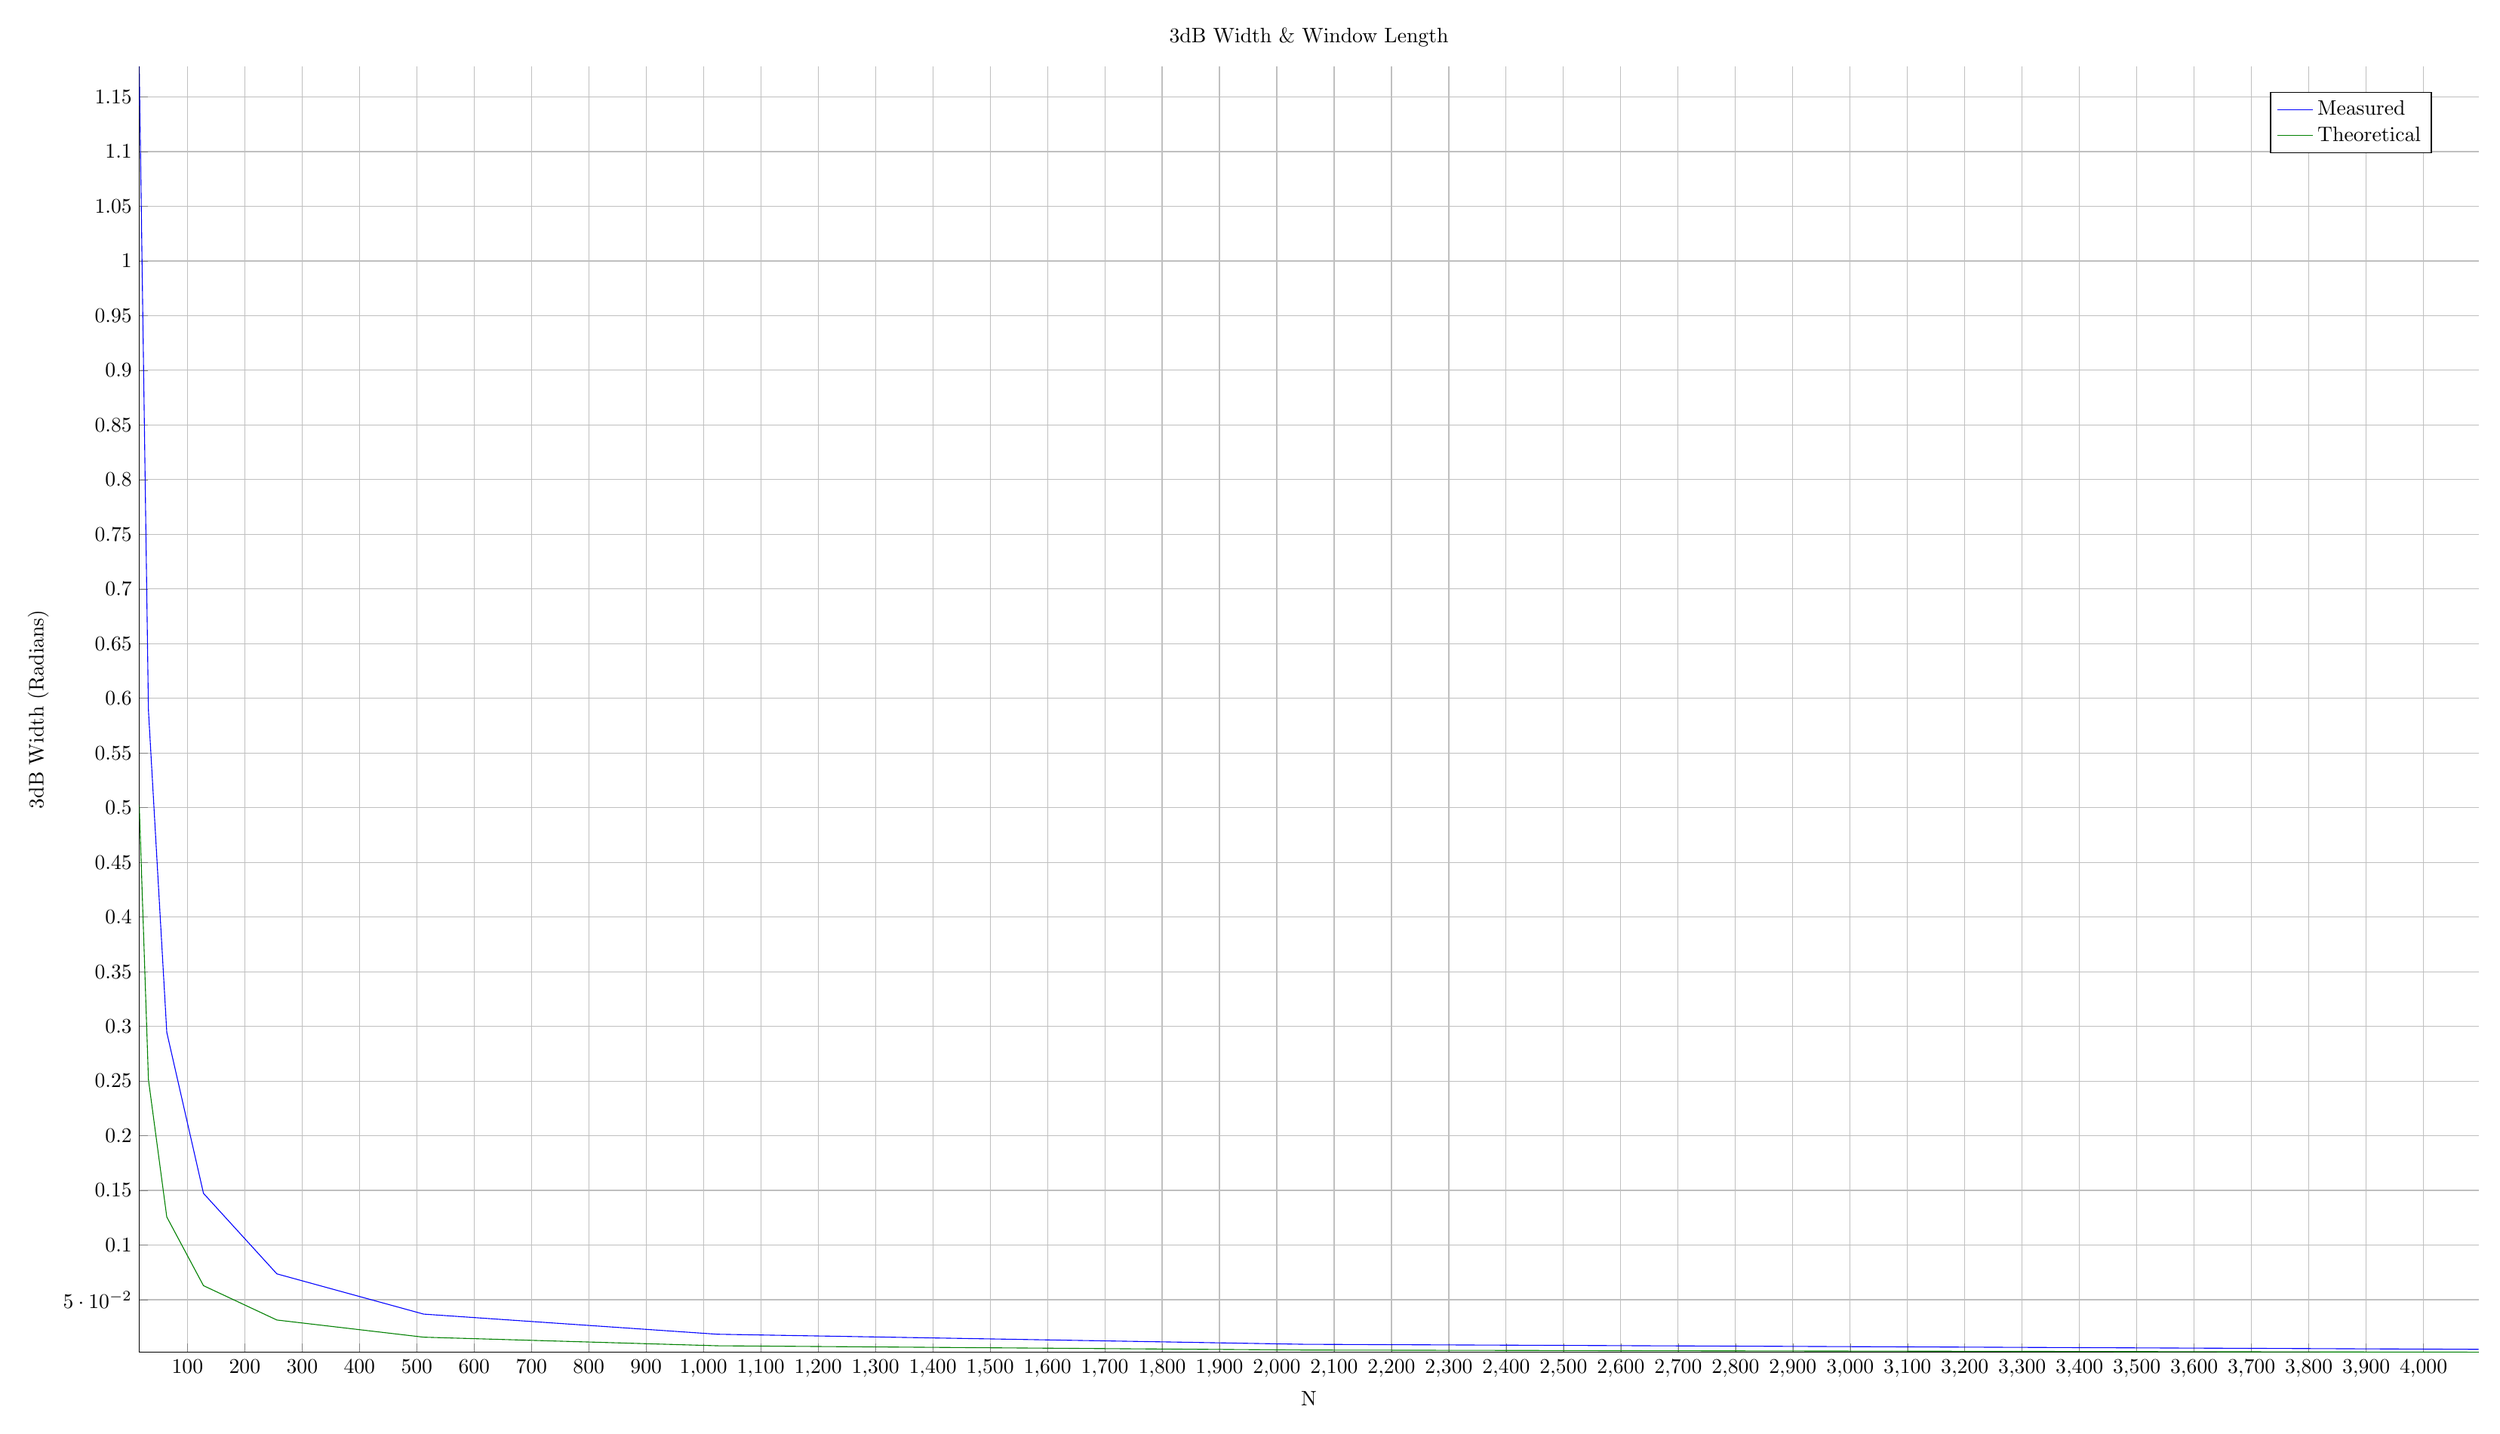
\begin{tikzpicture}

\begin{axis}[%
width=15.5in,
height=8.52354166666667in,
scale only axis,
xmin=16,
xmax=4096,
xlabel={N},
xmajorgrids,
ymin=0.00196349540849362,
ymax=1.17809724509617,
ylabel={3dB Width (Radians)},
ymajorgrids,
title={3dB Width \& Window Length},
axis x line*=bottom,
axis y line*=left,
legend style={draw=black,fill=white,legend cell align=left}
]
\addplot [color=blue,solid]
  table[row sep=crcr]{16	1.17809724509617\\
32	0.589048622548086\\
64	0.294524311274043\\
128	0.147262155637022\\
256	0.0736310778185108\\
512	0.0368155389092554\\
1024	0.0184077694546277\\
2048	0.00920388472731385\\
4096	0.00460194236365692\\
};
\addlegendentry{Measured};

\addplot [color=black!50!green,solid]
  table[row sep=crcr]{16	0.502654824574367\\
32	0.251327412287183\\
64	0.125663706143592\\
128	0.0628318530717959\\
256	0.0314159265358979\\
512	0.015707963267949\\
1024	0.00785398163397448\\
2048	0.00392699081698724\\
4096	0.00196349540849362\\
};
\addlegendentry{Theoretical};

\end{axis}
\end{tikzpicture}%}
		\captionof{figure}{\textit{Prediction Error Estimates for varying Model Orders}}
		\label{fig:}
%	\end{figure}
\end{minipage}
\begin{minipage}{.5\textwidth}
	%	\begin{figure}[h]
	\center
	\resizebox{\textwidth}{!}{% This file was created by matlab2tikz v0.4.7 (commit de21168db67fef7dc08f495c8f484b09a07aa02e) running on MATLAB 8.4.
% Copyright (c) 2008--2014, Nico Schlömer <nico.schloemer@gmail.com>
% All rights reserved.
% Minimal pgfplots version: 1.3
% 
% The latest updates can be retrieved from
%   http://www.mathworks.com/matlabcentral/fileexchange/22022-matlab2tikz
% where you can also make suggestions and rate matlab2tikz.
% 
%
% defining custom colors
\definecolor{mycolor1}{rgb}{0.00000,0.44700,0.74100}%
%
\begin{tikzpicture}

\begin{axis}[%
width=3in,
height=2in,
scale only axis,
every outer x axis line/.append style={white!15!black},
every x tick label/.append style={font=\color{white!15!black}},
xmin=16,
xmax=4096,
xlabel={N},
xmajorgrids,
every outer y axis line/.append style={white!15!black},
every y tick label/.append style={font=\color{white!15!black}},
tick align = outside,
ymin=13.178195824295,
ymax=13.4246672179578,
ylabel={Sidelobe Level (dB)},
ymajorgrids,
title style={font=\bfseries},
title={Sidelobe Level \& Window Length},
axis x line*=bottom,
axis y line*=left,
legend style={draw=black,fill=white,legend cell align=left}
]
\addplot [color=mycolor1,solid,forget plot]
  table[row sep=crcr]{16	13.178195824295\\
32	13.2497460511386\\
64	13.3427852124304\\
128	13.4003618622879\\
256	13.4246672179578\\
512	13.410416613703\\
1024	13.4035095429084\\
2048	13.4001094256601\\
4096	13.3984225829454\\
};
\end{axis}
\end{tikzpicture}%}
	\captionof{figure}{\textit{Prediction Error Estimates for varying Model Orders}}
	\label{fig:}
	%	\end{figure}
\end{minipage}


\subsubsection{Resolution Threshold}
\begin{figure}[h]
	\centering
	\begin{subfigure}[b]{0.23\textwidth}
		\resizebox{\textwidth}{!}{% This file was created by matlab2tikz v0.4.7 (commit fd1f91e81f99952e85a7de453e57b338734fa875) running on MATLAB 8.4.
% Copyright (c) 2008--2014, Nico Schlömer <nico.schloemer@gmail.com>
% All rights reserved.
% Minimal pgfplots version: 1.3
% 
% The latest updates can be retrieved from
%   http://www.mathworks.com/matlabcentral/fileexchange/22022-matlab2tikz
% where you can also make suggestions and rate matlab2tikz.
% 
%
% defining custom colors
\definecolor{mycolor1}{rgb}{0.00000,0.44700,0.74100}%
%
\begin{tikzpicture}

\begin{axis}[%
width=1.5in,
height=0.75in,
scale only axis,
every outer x axis line/.append style={white!15!black},
every x tick label/.append style={font=\color{white!15!black}},
xmin=0.54,
xmax=0.64,
xlabel={Normalised Frequency},
xmajorgrids,
every outer y axis line/.append style={white!15!black},
every y tick label/.append style={font=\color{white!15!black}},
tick align = outside,
ymin=0,
ymax=18000,
ylabel={Power},
ymajorgrids,
title style={font=\bfseries},
title={Periodogram, $\alpha=0.60$},
axis x line*=bottom,
axis y line*=left
]
\addplot [color=mycolor1,solid,forget plot]
  table[row sep=crcr]{-1	0.890696434330186\\
-0.99951171875	0.978440219563872\\
-0.9990234375	1.22832059687291\\
-0.99853515625	1.60231591152454\\
-0.998046875	2.04351867792528\\
-0.99755859375	2.48479399864423\\
-0.9970703125	2.85899441146608\\
-0.99658203125	3.10917719905623\\
-0.99609375	3.19726973746075\\
-0.99560546875	3.10986444528924\\
-0.9951171875	2.8602614480233\\
-0.99462890625	2.48644780845822\\
-0.994140625	2.04532029844522\\
-0.99365234375	1.60403018665697\\
-0.9931640625	1.22976646017185\\
-0.99267578125	0.979531653814417\\
-0.9921875	0.891465837088578\\
-0.99169921875	0.979039056724328\\
-0.9912109375	1.22899639514048\\
-0.99072265625	1.60336908326861\\
-0.990234375	2.04524658441161\\
-0.98974609375	2.48743231660781\\
-0.9892578125	2.86266675981304\\
-0.98876953125	3.11386289819739\\
-0.98828125	3.2027966519545\\
-0.98779296875	3.11592957018002\\
-0.9873046875	2.86647696502148\\
-0.98681640625	2.49240561878883\\
-0.986328125	2.05066438095871\\
-0.98583984375	1.60852421792462\\
-0.9853515625	1.23334436837326\\
-0.98486328125	0.982321198553059\\
-0.984375	0.893779571711831\\
-0.98388671875	0.981332465470654\\
-0.9833984375	1.23179870594479\\
-0.98291015625	1.60719726156755\\
-0.982421875	2.05051642381862\\
-0.98193359375	2.49438171057321\\
-0.9814453125	2.87130487601227\\
-0.98095703125	3.12395521672615\\
-0.98046875	3.21389021373787\\
-0.97998046875	3.12741619106722\\
-0.9794921875	2.87768567800867\\
-0.97900390625	2.50271030809328\\
-0.978515625	2.0595894026637\\
-0.97802734375	1.61583037512389\\
-0.9775390625	1.23908010077239\\
-0.97705078125	0.986828954174935\\
-0.9765625	0.897654303303549\\
-0.97607421875	0.985336952172552\\
-0.9755859375	1.23674769003925\\
-0.97509765625	1.61382799265345\\
-0.974609375	2.05936613603935\\
-0.97412109375	2.50569224474577\\
-0.9736328125	2.88497103244751\\
-0.97314453125	3.13952696070322\\
-0.97265625	3.23063050785091\\
-0.97216796875	3.14440728967986\\
-0.9716796875	2.89396862036242\\
-0.97119140625	2.51743643005454\\
-0.970703125	2.07215998408851\\
-0.97021484375	1.62600159456853\\
-0.9697265625	1.24701523575908\\
-0.96923828125	0.993087596750756\\
-0.96875	0.903118096210294\\
-0.96826171875	0.991081487139115\\
-0.9677734375	1.24387913259088\\
-0.96728515625	1.62330923930944\\
-0.966796875	2.07185978761422\\
-0.96630859375	2.52144588206944\\
-0.9658203125	2.90376436547553\\
-0.96533203125	3.16069120869325\\
-0.96484375	3.25313922724775\\
-0.96435546875	3.16702651448619\\
-0.9638671875	2.91544441632499\\
-0.96337890625	2.53669138601345\\
-0.962890625	2.08846790635324\\
-0.96240234375	1.63911221320681\\
-0.9619140625	1.25720780640744\\
-0.96142578125	1.00114289323617\\
-0.9609375	0.910210856028245\\
-0.96044921875	0.998607960171801\\
-0.9599609375	1.25324500550711\\
-0.95947265625	1.63571013491964\\
-0.958984375	2.08808858008684\\
-0.95849609375	2.54175777599994\\
-0.9580078125	2.92782244006561\\
-0.95751953125	3.18760309899133\\
-0.95703125	3.28158159892863\\
-0.95654296875	3.19544014060993\\
-0.9560546875	2.94227116404965\\
-0.95556640625	2.56061713240875\\
-0.955078125	2.10863357244204\\
-0.95458984375	1.65525915375286\\
-0.9541015625	1.26973322651115\\
-0.95361328125	1.0110544316682\\
-0.953125	0.91898496523652\\
-0.95263671875	1.00797184637998\\
-0.9521484375	1.26491429282162\\
-0.95166015625	1.65112208219088\\
-0.951171875	2.10817230166512\\
-0.95068359375	2.56677810673943\\
-0.9501953125	2.95732344755509\\
-0.94970703125	3.22046231284368\\
-0.94921875	3.31616903368118\\
-0.94873046875	3.22985974149462\\
-0.9482421875	2.97464898081282\\
-0.94775390625	2.58939247060665\\
-0.947265625	2.13280795311483\\
-0.94677734375	1.67456349384015\\
-0.9462890625	1.28468551288863\\
-0.94580078125	1.02289658671082\\
-0.9453125	0.929506130148208\\
-0.94482421875	1.01924310074028\\
-0.9443359375	1.27897410202405\\
-0.94384765625	1.66966022703243\\
-0.943359375	2.13226126253962\\
-0.94287109375	2.59669451308767\\
-0.9423828125	2.99248909788898\\
-0.94189453125	3.25951632316432\\
-0.94140625	3.35716257376896\\
-0.94091796875	3.27054564744589\\
-0.9404296875	3.01282328213675\\
-0.93994140625	2.62323598382161\\
-0.939453125	2.16117507257235\\
-0.93896484375	1.6971724637351\\
-0.9384765625	1.30217883869785\\
-0.93798828125	1.03675974798149\\
-0.9375	0.941854463175841\\
-0.93701171875	1.03250730666057\\
-0.9365234375	1.29553109267761\\
-0.93603515625	1.6914653492136\\
-0.935546875	2.16053876864224\\
-0.93505859375	2.63173518894427\\
-0.9345703125	3.0335882886898\\
-0.93408203125	3.30506450151517\\
-0.93359375	3.4048772373043\\
-0.93310546875	3.31781129039066\\
-0.9326171875	3.05708888928702\\
-0.93212890625	2.66240970598563\\
-0.931640625	2.19395510590221\\
-0.93115234375	1.72326193064879\\
-0.9306640625	1.32234946296345\\
-0.93017578125	1.05275184688939\\
-0.9296875	0.956125831792497\\
-0.92919921875	1.04786711172284\\
-0.9287109375	1.31471326353245\\
-0.92822265625	1.71670622441196\\
-0.927734375	2.1932242055051\\
-0.92724609375	2.6721727344614\\
-0.9267578125	3.08094165816709\\
-0.92626953125	3.35746320354458\\
-0.92578125	3.459687386885\\
-0.92529296875	3.37202856288311\\
-0.9248046875	3.1077950866015\\
-0.92431640625	2.70722363142915\\
-0.923828125	2.23140818052505\\
-0.92333984375	1.75303944383438\\
-0.9228515625	1.34535809404552\\
-0.92236328125	1.07100022764039\\
-0.921875	0.972433514370479\\
-0.92138671875	1.06544399317659\\
-0.9208984375	1.33667215104194\\
-0.92041015625	1.7455825276953\\
-0.919921875	2.23057682396664\\
-0.91943359375	2.71832887686158\\
-0.9189453125	3.13492715837754\\
-0.91845703125	3.41713198596492\\
-0.91796875	3.52203328473483\\
-0.91748046875	3.4336343539403\\
-0.9169921875	3.16535178268474\\
-0.91650390625	2.75804120326668\\
-0.916015625	2.27383899832264\\
-0.91552734375	1.78674793425297\\
-0.9150390625	1.37139275999363\\
-0.91455078125	1.09165392011456\\
-0.9140625	0.990910213747693\\
-0.91357421875	1.08538040712714\\
-0.9130859375	1.36158550634529\\
-0.91259765625	1.77832836717349\\
-0.912109375	2.27290034385187\\
-0.91162109375	2.77058020635621\\
-0.9111328125	3.19598682129464\\
-0.91064453125	3.48456114829606\\
-0.91015625	3.59242903897684\\
-0.90966796875	3.50313846662484\\
-0.9091796875	3.23023696948296\\
-0.90869140625	2.81528595407131\\
-0.908203125	2.32160242525581\\
-0.90771484375	1.82467018675863\\
-0.9072265625	1.40067227751204\\
-0.90673828125	1.11488638719511\\
-0.90625	1.01171049251541\\
-0.90576171875	1.10784238934284\\
-0.9052734375	1.38966053516526\\
-0.90478515625	1.81521655952492\\
-0.904296875	2.32054852174681\\
-0.90380859375	2.82936511008181\\
-0.9033203125	3.26463493450427\\
-0.90283203125	3.5603208422166\\
-0.90234375	3.67147219813295\\
-0.90185546875	3.58113317476177\\
-0.9013671875	3.30300572288042\\
-0.90087890625	2.87944951677912\\
-0.900390625	2.37511023276649\\
-0.89990234375	1.86713423285492\\
-0.8994140625	1.43345043466487\\
-0.89892578125	1.14089883764893\\
-0.8984375	1.03501371035936\\
-0.89794921875	1.1330226929532\\
-0.8974609375	1.42113780663656\\
-0.89697265625	1.85656378762103\\
-0.896484375	2.37393186628052\\
-0.89599609375	2.89519213364576\\
-0.8955078125	3.3414678986636\\
-0.89501953125	3.64507205332716\\
-0.89453125	3.75985531655283\\
-0.89404296875	3.66830474187977\\
-0.8935546875	3.38430105067335\\
-0.89306640625	2.95110127944712\\
-0.892578125	2.43483922237252\\
-0.89208984375	1.91451984995158\\
-0.8916015625	1.47002103192299\\
-0.89111328125	1.16992421898711\\
-0.890625	1.06102756434964\\
-0.89013671875	1.1611445701217\\
-0.8896484375	1.456295964187\\
-0.88916015625	1.90273681633259\\
-0.888671875	2.43352573126413\\
-0.88818359375	2.96865005867999\\
-0.8876953125	3.42717610863661\\
-0.88720703125	3.73957983837233\\
-0.88671875	3.85837989641384\\
-0.88623046875	3.76544730861425\\
-0.8857421875	3.47486697260284\\
-0.88525390625	3.03090002810771\\
-0.884765625	2.5013410246778\\
-0.88427734375	1.9672664011694\\
-0.8837890625	1.51072396360684\\
-0.88330078125	1.20223203435688\\
-0.8828125	1.08999235913648\\
-0.88232421875	1.19246633236222\\
-0.8818359375	1.49545740585015\\
-0.88134765625	1.95415998794675\\
-0.880859375	2.49988007645473\\
-0.88037109375	3.05042005934054\\
-0.8798828125	3.52255828877657\\
-0.87939453125	3.84472930038728\\
-0.87890625	3.96797321744059\\
-0.87841796875	3.87347966069851\\
-0.8779296875	3.57556431761322\\
-0.87744140625	3.11960801208634\\
-0.876953125	2.57525394042941\\
-0.87646484375	2.02588231127959\\
-0.8759765625	1.55595256971879\\
-0.87548828125	1.2381341654543\\
-0.875	1.12218616738468\\
-0.87451171875	1.22728685948719\\
-0.8740234375	1.53899514524769\\
-0.87353515625	2.01132427670261\\
-0.873046875	2.5736312618668\\
-0.87255859375	3.1412903963059\\
-0.8720703125	3.62853882651686\\
-0.87158203125	3.96154491198593\\
-0.87109375	4.08970870118917\\
-0.87060546875	3.99346552597902\\
-0.8701171875	3.6873898529814\\
-0.86962890625	3.2181079823763\\
-0.869140625	2.65731728987962\\
-0.86865234375	2.09095655383652\\
-0.8681640625	1.60616255007474\\
-0.86767578125	1.27799193240042\\
-0.8671875	1.15793108375788\\
-0.86669921875	1.26595227255842\\
-0.8662109375	1.58734112079884\\
-0.86572265625	2.07479825657938\\
-0.865234375	2.65551633952228\\
-0.86474609375	3.24217422998663\\
-0.8642578125	3.74618879506312\\
-0.86376953125	4.09121396196993\\
-0.86328125	4.22483063216266\\
-0.86279296875	4.12663822530263\\
-0.8623046875	3.81149952770798\\
-0.86181640625	3.32742390440569\\
-0.861328125	2.74838886475492\\
-0.86083984375	2.16317262784905\\
-0.8603515625	1.66188281317959\\
-0.85986328125	1.32222468522187\\
-0.859375	1.19760083166642\\
-0.85888671875	1.30886404520092\\
-0.8583984375	1.64099629389485\\
-0.85791015625	2.14524143346563\\
-0.857421875	2.74639043394904\\
-0.85693359375	3.35413129497698\\
-0.8564453125	3.87675154701945\\
-0.85595703125	4.23511511555561\\
-0.85546875	4.37478428699093\\
-0.85498046875	4.27443073259089\\
-0.8544921875	3.94923683191186\\
-0.85400390625	3.44874624382411\\
-0.853515625	2.84946624486619\\
-0.85302734375	2.24332563772954\\
-0.8525390625	1.72372873789846\\
-0.85205078125	1.37132030507253\\
-0.8515625	1.24163005517462\\
-0.85107421875	1.35648890475398\\
-0.8505859375	1.70054297240497\\
-0.85009765625	2.2234205196626\\
-0.849609375	2.84724796951417\\
-0.84912109375	3.47839438785912\\
-0.8486328125	4.02167401140788\\
-0.84814453125	4.39485336104639\\
-0.84765625	4.54125282395469\\
-0.84716796875	4.43851250276139\\
-0.8466796875	4.10216756298666\\
-0.84619140625	3.58346298416143\\
-0.845703125	2.96171296285469\\
-0.84521484375	2.33234326918762\\
-0.8447265625	1.7924184656242\\
-0.84423828125	1.42584810373382\\
-0.84375	1.2905257251276\\
-0.84326171875	1.40937097645644\\
-0.8427734375	1.76665992195626\\
-0.84228515625	2.31022939594184\\
-0.841796875	2.95924872283314\\
-0.84130859375	3.61640189807755\\
-0.8408203125	4.18264515808408\\
-0.84033203125	4.57230298992614\\
-0.83984375	4.72620268422025\\
-0.83935546875	4.6208348287072\\
-0.8388671875	4.27212267320833\\
-0.83837890625	3.73319788124557\\
-0.837890625	3.08649079533943\\
-0.83740234375	2.43131169209287\\
-0.8369140625	1.86879302676385\\
-0.83642578125	1.48647475704155\\
-0.8359375	1.34488121722174\\
-0.83544921875	1.46814675908825\\
-0.8349609375	1.8401409949741\\
-0.83447265625	2.40671372879684\\
-0.833984375	3.08374997154824\\
-0.83349609375	3.76983798156796\\
-0.8330078125	4.36164353592907\\
-0.83251953125	4.7696607571565\\
-0.83203125	4.93193978988971\\
-0.83154296875	4.8236870275291\\
-0.8310546875	4.46125138812032\\
-0.83056640625	3.89985792362845\\
-0.830078125	3.22539985473797\\
-0.82958984375	2.54150774186559\\
-0.8291015625	1.95384135582439\\
-0.82861328125	1.55398410582865\\
-0.828125	1.40539379265936\\
-0.82763671875	1.53356370194402\\
-0.8271484375	1.92191823213844\\
-0.82666015625	2.51410150889817\\
-0.826171875	3.22234640426768\\
-0.82568359375	3.94068247417431\\
-0.8251953125	4.56099638659467\\
-0.82470703125	4.98951204195478\\
-0.82421875	5.16117954401981\\
-0.82373046875	5.04976648417429\\
-0.8232421875	4.67208748088633\\
-0.82275390625	4.08569259685608\\
-0.822265625	3.38032869266117\\
-0.82177734375	2.66443916571507\\
-0.8212890625	2.0487315892784\\
-0.82080078125	1.62930192655024\\
-0.8203125	1.47288644637784\\
-0.81982421875	1.60650339859792\\
-0.8193359375	2.013090694871\\
-0.81884765625	2.63384118070059\\
-0.818359375	3.37691998980059\\
-0.81787109375	4.1312733168669\\
-0.8173828125	4.78345364469525\\
-0.81689453125	5.23491374574767\\
-0.81640625	5.41713461877407\\
-0.81591796875	5.30226657366728\\
-0.8154296875	4.90763253823498\\
-0.81494140625	4.29336840902741\\
-0.814453125	3.55351736051528\\
-0.81396484375	2.80189531593675\\
-0.8134765625	2.15485050658324\\
-0.81298828125	1.71352714206387\\
-0.8125	1.54833540877424\\
-0.81201171875	1.68801074865283\\
-0.8115234375	2.11496070271472\\
-0.81103515625	2.76764958526119\\
-0.810546875	3.54970273363278\\
-0.81005859375	4.34438518963786\\
-0.8095703125	5.03228124551278\\
-0.80908203125	5.50949892311613\\
-0.80859375	5.70362586753223\\
-0.80810546875	5.58498785111138\\
-0.8076171875	5.17146136463361\\
-0.80712890625	4.52606332233999\\
-0.806640625	3.7476373889872\\
-0.80615234375	2.95601149742447\\
-0.8056640625	2.27385362057105\\
-0.80517578125	1.80797145319849\\
-0.8046875	1.63290503080784\\
-0.80419921875	1.77933090234826\\
-0.8037109375	2.22907972264348\\
-0.80322265625	2.91757270091193\\
-0.802734375	3.74335625887255\\
-0.80224609375	4.58332933181981\\
-0.8017578125	5.31137970105806\\
-0.80126953125	5.81760989041878\\
-0.80078125	6.02522357407392\\
-0.80029296875	5.90247980409553\\
-0.7998046875	5.46785649996206\\
-0.79931640625	4.78758739361496\\
-0.798828125	3.9658940691276\\
-0.79833984375	3.12935133167908\\
-0.7978515625	2.40772932844121\\
-0.79736328125	1.91421008649369\\
-0.796875	1.7279924034425\\
-0.79638671875	1.88195645035561\\
-0.7958984375	2.35730695712002\\
-0.79541015625	3.08606323118352\\
-0.794921875	3.96107355997771\\
-0.79443359375	4.85208132013634\\
-0.7939453125	5.62543606482687\\
-0.79345703125	6.16446901334676\\
-0.79296875	6.38742889291453\\
-0.79248046875	6.2602231467514\\
-0.7919921875	5.8019814061623\\
-0.79150390625	5.08253827009247\\
-0.791015625	4.21215842864051\\
-0.79052734375	3.32501313624841\\
-0.7900390625	2.55888181790422\\
-0.78955078125	2.03414736683407\\
-0.7890625	1.8352849415909\\
-0.78857421875	1.99768823583636\\
-0.7880859375	2.50188480686039\\
-0.78759765625	3.27608059366312\\
-0.787109375	4.20671027400002\\
-0.78662109375	5.15544611756674\\
-0.7861328125	5.98012047112639\\
-0.78564453125	6.55639986769958\\
-0.78515625	6.79690909623353\\
-0.78466796875	6.6648664643783\\
-0.7841796875	6.18010556494623\\
-0.78369140625	5.41650354018262\\
-0.783203125	4.49113917906991\\
-0.78271484375	3.5467686674009\\
-0.7822265625	2.73023926639405\\
-0.78173828125	2.17010227901778\\
-0.78125	1.95683542330717\\
-0.78076171875	2.12871447460552\\
-0.7802734375	2.66553699846392\\
-0.77978515625	3.49122101556909\\
-0.779296875	4.48495567464914\\
-0.77880859375	5.49927335458399\\
-0.7783203125	6.38234284314431\\
-0.77783203125	7.00111649971895\\
-0.77734375	7.26180567093248\\
-0.77685546875	7.12453655378883\\
-0.7763671875	6.60990006719075\\
-0.77587890625	5.79632680310741\\
-0.775390625	4.80860909699734\\
-0.77490234375	3.79924599147743\\
-0.7744140625	2.92539655590645\\
-0.77392578125	2.32492130139052\\
-0.7734375	2.09516080729075\\
-0.77294921875	2.27771476723983\\
-0.7724609375	2.85159750595342\\
-0.77197265625	3.73588856259362\\
-0.771484375	4.80155774949209\\
-0.77099609375	5.89074111404339\\
-0.7705078125	6.84059179206393\\
-0.77001953125	7.50810586418455\\
-0.76953125	7.79214225488369\\
-0.76904296875	7.64924992346235\\
-0.7685546875	7.1008301181386\\
-0.76806640625	6.23046148106481\\
-0.767578125	5.17170647669736\\
-0.76708984375	4.08817329752465\\
-0.7666015625	3.14880569471028\\
-0.76611328125	2.50212892674302\\
-0.765625	2.25337385486498\\
-0.76513671875	2.44799838002001\\
-0.7646484375	3.06418183378501\\
-0.76416015625	4.01552251950521\\
-0.763671875	5.16362284535833\\
-0.76318359375	6.33873433427153\\
-0.7626953125	7.36538724511889\\
-0.76220703125	8.0891394242758\\
-0.76171875	8.4003712120288\\
-0.76123046875	8.25146501031021\\
-0.7607421875	7.66468258832603\\
-0.76025390625	6.72944710393316\\
-0.759765625	5.58934154218724\\
-0.75927734375	4.42070803831293\\
-0.7587890625	3.40603309973013\\
-0.75830078125	2.70613099039614\\
-0.7578125	2.43536063472078\\
-0.75732421875	2.64369034725481\\
-0.7568359375	3.30841736401563\\
-0.75634765625	4.33690340503964\\
-0.755859375	5.5800195402592\\
-0.75537109375	6.85435571885514\\
-0.7548828125	7.96989265799619\\
-0.75439453125	8.75896634385799\\
-0.75390625	9.10211549681878\\
-0.75341796875	8.94683298716332\\
-0.7529296875	8.31628450984338\\
-0.75244140625	7.30655908388835\\
-0.751953125	6.0727518082033\\
-0.75146484375	4.80588735468635\\
-0.7509765625	3.70411201041389\\
-0.75048828125	2.94249311780388\\
-0.75	2.64602316989898\\
-0.74951171875	2.86998529837649\\
-0.7490234375	3.59075727114513\\
-0.74853515625	4.70857034131144\\
-0.748046875	6.06193037916842\\
-0.74755859375	7.45162502866829\\
-0.7470703125	8.6707545952971\\
-0.74658203125	9.53626595471977\\
-0.74609375	9.91718993290232\\
-0.74560546875	9.75523329480267\\
-0.7451171875	9.07449589715108\\
-0.74462890625	7.97870824332808\\
-0.744140625	6.63627228680381\\
-0.74365234375	5.25525374498952\\
-0.7431640625	4.05203251536871\\
-0.74267578125	3.21832781258084\\
-0.7421875	2.8916160963787\\
-0.74169921875	3.13349875493304\\
-0.7412109375	3.91941458081109\\
-0.74072265625	5.14139866910448\\
-0.740234375	6.62361681962681\\
-0.73974609375	8.14845064104353\\
-0.7392578125	9.48927170444991\\
-0.73876953125	10.4449767202762\\
-0.73828125	10.871029164465\\
-0.73779296875	10.7022245147249\\
-0.7373046875	9.96360363788596\\
-0.73681640625	8.76770630237165\\
-0.736328125	7.29842118178955\\
-0.73583984375	5.78373856305953\\
-0.7353515625	4.46143429329268\\
-0.73486328125	3.54284154453475\\
-0.734375	3.18022145768498\\
-0.73388671875	3.4427612100354\\
-0.7333984375	4.30497201624645\\
-0.73291015625	5.6494122716569\\
-0.732421875	7.28349714971923\\
-0.73193359375	8.96800180100057\\
-0.7314453125	10.4530497259746\\
-0.73095703125	11.5161821735398\\
-0.73046875	11.9967187475964\\
-0.72998046875	11.8211127772374\\
-0.7294921875	11.0153131794962\\
-0.72900390625	9.70207816870932\\
-0.728515625	8.0834580907946\\
-0.72802734375	6.41093248105862\\
-0.7275390625	4.9476040201793\\
-0.72705078125	3.92812225331337\\
-0.7265625	3.52243053818734\\
-0.72607421875	3.80892548877997\\
-0.7255859375	4.76125407322255\\
-0.72509765625	6.25094642405664\\
-0.724609375	8.06569296021168\\
-0.72412109375	9.94068246984731\\
-0.7236328125	11.5983883646199\\
-0.72314453125	12.7908379375895\\
-0.72265625	13.3379395985703\\
-0.72216796875	13.1559579167905\\
-0.7216796875	12.2716504816\\
-0.72119140625	10.8197091081497\\
-0.720703125	9.0236655469207\\
-0.72021484375	7.16294972223567\\
-0.7197265625	5.5309409858344\\
-0.71923828125	4.39029623971204\\
-0.71875	3.93234291888971\\
-0.71826171875	4.24679966437829\\
-0.7177734375	5.30659874876413\\
-0.71728515625	6.97034554607226\\
-0.716796875	9.00229259039875\\
-0.71630859375	11.1070286759539\\
-0.7158203125	12.9737952903982\\
-0.71533203125	14.3237982356609\\
-0.71484375	14.9533280229498\\
-0.71435546875	14.766037500005\\
-0.7138671875	13.7892834485643\\
-0.71337890625	12.1717977801324\\
-0.712890625	10.1627652699742\\
-0.71240234375	8.07522617264962\\
-0.7119140625	6.23916038326587\\
-0.71142578125	4.95126691089594\\
-0.7109375	4.42906368551052\\
-0.71044921875	4.77638904727354\\
-0.7099609375	5.96575310227266\\
-0.70947265625	7.84049708025655\\
-0.708984375	10.1367387536988\\
-0.70849609375	12.5220590957411\\
-0.7080078125	14.6452803082493\\
-0.70751953125	16.1899021830993\\
-0.70703125	16.92308744418\\
-0.70654296875	16.732637866138\\
-0.7060546875	15.6461168725304\\
-0.70556640625	13.8289079096055\\
-0.705078125	11.5611639730023\\
-0.70458984375	9.19682764108019\\
-0.7041015625	7.11069180463506\\
-0.70361328125	5.64139608395062\\
-0.703125	5.03900485894961\\
-0.70263671875	5.4252560846677\\
-0.7021484375	6.7727690401443\\
-0.70166015625	8.90670808313704\\
-0.701171875	11.5290277673897\\
-0.70068359375	14.2619770938008\\
-0.7001953125	16.7045419933316\\
-0.69970703125	18.4934205244082\\
-0.69921875	19.3592883303677\\
-0.69873046875	19.1696716707377\\
-0.6982421875	17.9516404047178\\
-0.69775390625	15.8904975878929\\
-0.697265625	13.304242133436\\
-0.69677734375	10.5972781451072\\
-0.6962890625	8.20007667175464\\
-0.69580078125	6.50376141767423\\
-0.6953125	5.7995265242393\\
-0.69482421875	6.23223529650495\\
-0.6943359375	7.77555215583917\\
-0.69384765625	10.2328048196752\\
-0.693359375	13.2639200845411\\
-0.69287109375	16.4347997757957\\
-0.6923828125	19.2820078522023\\
-0.69189453125	21.3831674593394\\
-0.69140625	22.4224140431469\\
-0.69091796875	22.2408045460898\\
-0.6904296875	20.8636888784407\\
-0.68994140625	18.5004163146866\\
-0.689453125	15.5158866262953\\
-0.68896484375	12.3777472814969\\
-0.6884765625	9.58683228913751\\
-0.68798828125	7.60114689575146\\
-0.6875	6.76489112870158\\
-0.68701171875	7.2534730875601\\
-0.6865234375	9.04323856518433\\
-0.68603515625	11.911042997203\\
-0.685546875	15.4643366382372\\
-0.68505859375	19.1977865743876\\
-0.6845703125	22.5683245580736\\
-0.68408203125	25.077528600934\\
-0.68359375	26.3488968833532\\
-0.68310546875	26.1880940537361\\
-0.6826171875	24.6166014649477\\
-0.68212890625	21.8730637545479\\
-0.681640625	18.3814372527722\\
-0.68115234375	14.6900971548353\\
-0.6806640625	11.3905850944483\\
-0.68017578125	9.02797566745912\\
-0.6796875	8.01638067273027\\
-0.67919921875	8.57262072190155\\
-0.6787109375	10.6786059966129\\
-0.67822265625	14.0788169439656\\
-0.677734375	18.3140578230787\\
-0.67724609375	22.7871430015904\\
-0.6767578125	26.8512014609905\\
-0.67626953125	29.9076193062104\\
-0.67578125	31.4988713200926\\
-0.67529296875	31.3819333085062\\
-0.6748046875	29.5706004049169\\
-0.67431640625	26.3395117275176\\
-0.673828125	22.1883594934775\\
-0.67333984375	17.77080380461\\
-0.6728515625	13.7981106897204\\
-0.67236328125	10.9316303728526\\
-0.671875	9.68027747044063\\
-0.67138671875	10.3188043114191\\
-0.6708984375	12.8398711214337\\
-0.67041015625	16.9480783930022\\
-0.669921875	22.0979242145653\\
-0.66943359375	27.5709937109876\\
-0.6689453125	32.581581349906\\
-0.66845703125	36.3953331795142\\
-0.66796875	38.4431149984704\\
-0.66748046875	38.41258293695\\
-0.6669921875	36.302881252859\\
-0.66650390625	32.4331381616739\\
-0.666015625	27.4022350581249\\
-0.66552734375	22.0046924689905\\
-0.6650390625	17.1143409942343\\
-0.66455078125	13.5526744981741\\
-0.6640625	11.9615778857251\\
-0.66357421875	12.6999925422353\\
-0.6630859375	15.7809697160086\\
-0.66259765625	20.8598581818661\\
-0.662109375	27.2768740137355\\
-0.66162109375	34.1490980342897\\
-0.6611328125	40.4992681439221\\
-0.66064453125	45.4027613406283\\
-0.66015625	48.130849900558\\
-0.65966796875	48.2682467885765\\
-0.6591796875	45.7862303565213\\
-0.65869140625	41.0588567072251\\
-0.658203125	34.8180706371973\\
-0.65771484375	28.0527126684671\\
-0.6572265625	21.865121069666\\
-0.65673828125	17.3059079552881\\
-0.65625	15.2114480253626\\
-0.65576171875	16.0689675947434\\
-0.6552734375	19.9306969583118\\
-0.65478515625	26.3917543688856\\
-0.654296875	34.637191392456\\
-0.65380859375	43.5532722994399\\
-0.6533203125	51.888120230109\\
-0.65283203125	58.4388609556004\\
-0.65234375	62.2376067552886\\
-0.65185546875	62.707878273423\\
-0.6513671875	59.7666061977091\\
-0.65087890625	53.8542915264271\\
-0.650390625	45.8862357800822\\
-0.64990234375	37.129512853698\\
-0.6494140625	29.0218097557991\\
-0.64892578125	22.9576695802955\\
-0.6484375	20.0735325039856\\
-0.64794921875	21.0642791979878\\
-0.6474609375	26.0603781351212\\
-0.64697265625	34.5865948810974\\
-0.646484375	45.6116064872033\\
-0.64599609375	57.6844077637494\\
-0.6455078125	69.1400644829543\\
-0.64501953125	78.3461794833513\\
-0.64453125	83.9541599421932\\
-0.64404296875	85.1172525042321\\
-0.6435546875	81.640862418738\\
-0.64306640625	74.0395744421727\\
-0.642578125	63.4884113517471\\
-0.64208984375	51.671387895536\\
-0.6416015625	40.5461005051265\\
-0.64111328125	32.0565815719816\\
-0.640625	27.8358239613273\\
-0.64013671875	28.9426919888022\\
-0.6396484375	35.6746417980709\\
-0.63916015625	47.4879989548985\\
-0.638671875	63.0426705825969\\
-0.63818359375	80.3701160708587\\
-0.6376953125	97.1447363261919\\
-0.63720703125	111.022337871117\\
-0.63671875	119.997550855449\\
-0.63623046875	122.726999881073\\
-0.6357421875	118.767700922958\\
-0.63525390625	108.690535105412\\
-0.634765625	94.045530511862\\
-0.63427734375	77.1768459946791\\
-0.6337890625	60.9078394288911\\
-0.63330078125	48.1371291802565\\
-0.6328125	41.401973820547\\
-0.63232421875	42.4730642038415\\
-0.6318359375	52.0434192471309\\
-0.63134765625	69.5632606387198\\
-0.630859375	93.2536485580134\\
-0.63037109375	120.306701699591\\
-0.6298828125	147.252793078127\\
-0.62939453125	170.449131786463\\
-0.62890625	186.623516206365\\
-0.62841796875	193.395093732165\\
-0.6279296875	189.692902774372\\
-0.62744140625	176.003544316709\\
-0.626953125	154.400614466612\\
-0.62646484375	128.338000694772\\
-0.6259765625	102.222954306088\\
-0.62548828125	80.8183172151998\\
-0.625	68.5515169485967\\
-0.62451171875	68.8265538504848\\
-0.6240234375	83.4409375299372\\
-0.62353515625	112.200804062098\\
-0.623046875	152.804662603739\\
-0.62255859375	201.031811613063\\
-0.6220703125	251.229655800574\\
-0.62158203125	297.050461820626\\
-0.62109375	332.348613185501\\
-0.62060546875	352.120020165306\\
-0.6201171875	353.350790386806\\
-0.61962890625	335.645552123126\\
-0.619140625	301.527615102802\\
-0.61865234375	256.341594739141\\
-0.6181640625	207.739948513028\\
-0.61767578125	164.791859971401\\
-0.6171875	136.808633032766\\
-0.61669921875	132.026544288601\\
-0.6162109375	156.319028553027\\
-0.61572265625	212.119967402138\\
-0.615234375	297.72605945988\\
-0.61474609375	407.109127504516\\
-0.6142578125	530.312221992076\\
-0.61376953125	654.432776945981\\
-0.61328125	765.120239015841\\
-0.61279296875	848.444015809792\\
-0.6123046875	892.92969656184\\
-0.61181640625	891.525412017111\\
-0.611328125	843.251645103193\\
-0.61083984375	754.309265959391\\
-0.6103515625	638.470844022\\
-0.60986328125	516.654508786029\\
-0.609375	415.669716950068\\
-0.60888671875	366.219875666028\\
-0.6083984375	400.336447310929\\
-0.60791015625	548.49183735302\\
-0.607421875	836.684697137425\\
-0.60693359375	1283.80486509033\\
-0.6064453125	1899.56345994573\\
-0.60595703125	2683.218310302\\
-0.60546875	3623.24177511203\\
-0.60498046875	4697.97640579403\\
-0.6044921875	5877.21557417744\\
-0.60400390625	7124.54391296584\\
-0.603515625	8400.18842039205\\
-0.60302734375	9664.07554804126\\
-0.6025390625	10878.7693640134\\
-0.60205078125	12011.9835859627\\
-0.6015625	13038.4139436154\\
-0.60107421875	13940.7205997466\\
-0.6005859375	14709.5932284607\\
-0.60009765625	15342.9413774765\\
-0.599609375	15844.356565487\\
-0.59912109375	16221.0775506794\\
-0.5986328125	16481.7460058154\\
-0.59814453125	16634.2596790901\\
-0.59765625	16684.0116623199\\
-0.59716796875	16632.7500063285\\
-0.5966796875	16478.2084313019\\
-0.59619140625	16214.5566873476\\
-0.595703125	15833.6109457325\\
-0.59521484375	15326.6438952768\\
-0.5947265625	14686.5534986929\\
-0.59423828125	13910.0986662391\\
-0.59375	12999.8957460618\\
-0.59326171875	11965.893538071\\
-0.5927734375	10826.1036335925\\
-0.59228515625	9606.45005672632\\
-0.591796875	8339.70680005974\\
-0.59130859375	7063.60117159573\\
-0.5908203125	5818.26164211851\\
-0.59033203125	4643.26894905702\\
-0.58984375	3574.61900566344\\
-0.58935546875	2641.91984637315\\
-0.5888671875	1866.12098111868\\
-0.58837890625	1258.01523602366\\
-0.587890625	817.667626853893\\
-0.58740234375	534.823413870566\\
-0.5869140625	390.240452786818\\
-0.58642578125	357.791865192589\\
-0.5859375	407.105301048876\\
-0.58544921875	506.453517243111\\
-0.5849609375	625.592957734059\\
-0.58447265625	738.263687201946\\
-0.583984375	824.112440132786\\
-0.58349609375	869.87405170947\\
-0.5830078125	869.73570687774\\
-0.58251953125	824.90229572427\\
-0.58203125	742.468538921528\\
-0.58154296875	633.774475077113\\
-0.5810546875	512.467769297666\\
-0.58056640625	392.514696756718\\
-0.580078125	286.390782904845\\
-0.57958984375	203.644723374659\\
-0.5791015625	149.971228799738\\
-0.57861328125	126.857944389158\\
-0.578125	131.797819454929\\
-0.57763671875	158.990426955742\\
-0.5771484375	200.401737355722\\
-0.57666015625	247.017575020348\\
-0.576171875	290.114499589363\\
-0.57568359375	322.383208259958\\
-0.5751953125	338.770918129541\\
-0.57470703125	336.955355977817\\
-0.57421875	317.417160097816\\
-0.57373046875	283.132249071509\\
-0.5732421875	238.953948625048\\
-0.57275390625	190.790548060698\\
-0.572265625	144.703577397543\\
-0.57177734375	106.053893396326\\
-0.5712890625	78.8074983388181\\
-0.57080078125	65.0839326975099\\
-0.5703125	64.9917897520793\\
-0.56982421875	76.7540592697783\\
-0.5693359375	97.0864334756965\\
-0.56884765625	121.759586539892\\
-0.568359375	146.255663764888\\
-0.56787109375	166.421939296323\\
-0.5673828125	179.031029825329\\
-0.56689453125	182.175525407258\\
-0.56640625	175.452208651418\\
-0.56591796875	159.922939535185\\
-0.5654296875	137.871142676502\\
-0.56494140625	112.400257507798\\
-0.564453125	86.9399508859332\\
-0.56396484375	64.7350836250511\\
-0.5634765625	48.3906378356109\\
-0.56298828125	39.5338793405462\\
-0.5625	38.6351442669467\\
-0.56201171875	45.003992695749\\
-0.5615234375	56.9517612203483\\
-0.56103515625	72.0884327948016\\
-0.560546875	87.7043458137894\\
-0.56005859375	101.177751330217\\
-0.5595703125	110.34855232561\\
-0.55908203125	113.806387275809\\
-0.55859375	111.056034128004\\
-0.55810546875	102.542476910842\\
-0.5576171875	89.5389309949074\\
-0.55712890625	73.920610982099\\
-0.556640625	57.8623404203072\\
-0.55615234375	43.5072526487278\\
-0.5556640625	32.6557904868622\\
-0.55517578125	26.5190222656957\\
-0.5546875	25.5690135476444\\
-0.55419921875	29.5035117796374\\
-0.5537109375	37.3249191108082\\
-0.55322265625	47.5170059857669\\
-0.552734375	58.289397414606\\
-0.55224609375	67.8513446572325\\
-0.5517578125	74.6736986817218\\
-0.55126953125	77.7014561234249\\
-0.55078125	76.4880057346231\\
-0.55029296875	71.2347820605102\\
-0.5498046875	62.7344602371885\\
-0.54931640625	52.2299398156183\\
-0.548828125	41.2131349647118\\
-0.54833984375	31.1953999013563\\
-0.5478515625	23.4842934050269\\
-0.54736328125	18.9990984287082\\
-0.546875	18.1505923941478\\
-0.54638671875	20.8001928118191\\
-0.5458984375	26.3014200336998\\
-0.54541015625	33.6144653263191\\
-0.544921875	41.4742973032034\\
-0.54443359375	48.5856263864654\\
-0.5439453125	53.8150948227326\\
-0.54345703125	56.3525494375073\\
-0.54296875	55.8188091801528\\
-0.54248046875	52.3060035663757\\
-0.5419921875	46.3469551787894\\
-0.54150390625	38.8206280133563\\
-0.541015625	30.8098145175218\\
-0.54052734375	23.4336956474814\\
-0.5400390625	17.6808252154954\\
-0.53955078125	14.2671545507015\\
-0.5390625	13.5391925436526\\
-0.53857421875	15.4350722874836\\
-0.5380859375	19.5073365528268\\
-0.53759765625	25.0020296565243\\
-0.537109375	30.9805569785734\\
-0.53662109375	36.4649045341688\\
-0.5361328125	40.5839903434105\\
-0.53564453125	42.699464869271\\
-0.53515625	42.4930029173756\\
-0.53466796875	40.0033859320542\\
-0.5341796875	35.6094612002258\\
-0.53369140625	29.9631882090253\\
-0.533203125	23.8842344088729\\
-0.53271484375	18.2329199830573\\
-0.5322265625	13.7810043958504\\
-0.53173828125	11.0995383870126\\
-0.53125	10.479901704548\\
-0.53076171875	11.8987513959117\\
-0.5302734375	15.0307823355208\\
-0.52978515625	19.3060008287939\\
-0.529296875	24.0017090194362\\
-0.52880859375	28.3545339922527\\
-0.5283203125	31.6752835032807\\
-0.52783203125	33.4494821426463\\
-0.52734375	33.4090528104938\\
-0.52685546875	31.5653009586615\\
-0.5263671875	28.199380255998\\
-0.52587890625	23.8128394876318\\
-0.525390625	19.0467091460828\\
-0.52490234375	14.5820293063574\\
-0.5244140625	11.0371276391053\\
-0.52392578125	8.87702564474304\\
-0.5234375	8.34813467878871\\
-0.52294921875	9.44729072442948\\
-0.5224609375	11.9288285938047\\
-0.52197265625	15.3476386692669\\
-0.521484375	19.1308479967701\\
-0.52099609375	22.6666980142063\\
-0.5205078125	25.396926232366\\
-0.52001953125	26.898789116282\\
-0.51953125	26.9447602025093\\
-0.51904296875	25.5315668959957\\
-0.5185546875	22.8750082288899\\
-0.51806640625	19.3721847268264\\
-0.517578125	15.5375884096552\\
-0.51708984375	11.9232383990668\\
-0.5166015625	9.0351759524618\\
-0.51611328125	7.2588744770254\\
-0.515625	6.80448497763938\\
-0.51513671875	7.67961417530739\\
-0.5146484375	9.69303928633427\\
-0.51416015625	12.4880651664745\\
-0.513671875	15.5998357422713\\
-0.51318359375	18.5274698971732\\
-0.5126953125	20.8098928794851\\
-0.51220703125	22.0939422254415\\
-0.51171875	22.1847461410777\\
-0.51123046875	21.07125126408\\
-0.5107421875	18.9236529265548\\
-0.51025390625	16.0637535683625\\
-0.509765625	12.9132974332639\\
-0.50927734375	9.92850756082284\\
-0.5087890625	7.53092904893901\\
-0.50830078125	6.04500927898422\\
-0.5078125	5.65160688089486\\
-0.50732421875	6.36403615856242\\
-0.5068359375	8.02973802718891\\
-0.50634765625	10.3567675844506\\
-0.505859375	12.9605932796751\\
-0.50537109375	15.4237608373735\\
-0.5048828125	17.3592099987234\\
-0.50439453125	18.4676823986208\\
-0.50390625	18.5807466989902\\
-0.50341796875	17.6832994726332\\
-0.5029296875	15.9126024351593\\
-0.50244140625	13.5344915076343\\
-0.501953125	10.9007985405239\\
-0.50146484375	8.39475657461521\\
-0.5009765625	6.37281983244818\\
-0.50048828125	5.11169378239368\\
-0.5	4.76841054924636\\
-0.49951171875	5.35917118076008\\
-0.4990234375	6.75974842512489\\
-0.49853515625	8.72695627489429\\
-0.498046875	10.9375448346364\\
-0.49755859375	13.038339497007\\
-0.4970703125	14.6998801394706\\
-0.49658203125	15.6654439221208\\
-0.49609375	15.7881866528293\\
-0.49560546875	15.0510612129206\\
-0.4951171875	13.5668582808316\\
-0.49462890625	11.5587473377223\\
-0.494140625	9.3246136866464\\
-0.49365234375	7.19085500087079\\
-0.4931640625	5.46277441073611\\
-0.49267578125	4.37908247622968\\
-0.4921875	4.07726204027159\\
-0.49169921875	4.57479287667093\\
-0.4912109375	5.76875930286207\\
-0.49072265625	7.45355772087983\\
-0.490234375	9.35370928758049\\
-0.48974609375	11.166570484093\\
-0.4892578125	12.6083438770907\\
-0.48876953125	13.4564163675685\\
-0.48828125	13.5817304878575\\
-0.48779296875	12.9665050255431\\
-0.4873046875	11.7049059824246\\
-0.48681640625	9.98687274234256\\
-0.486328125	8.06783092436475\\
-0.48583984375	6.22909497087154\\
-0.4853515625	4.73507723166986\\
-0.48486328125	3.79379234133819\\
-0.484375	3.52653672620465\\
-0.48388671875	3.95114166582685\\
-0.4833984375	4.9810820375573\\
-0.48291015625	6.44030041512052\\
-0.482421875	8.09124657697235\\
-0.48193359375	9.67168894762776\\
-0.4814453125	10.9346117972323\\
-0.48095703125	11.6851448677252\\
-0.48046875	11.8090207877837\\
-0.47998046875	11.2884223137807\\
-0.4794921875	10.2030470488113\\
-0.47900390625	8.71647653377755\\
-0.478515625	7.05014515246007\\
-0.47802734375	5.44903114942334\\
-0.4775390625	4.14436902221121\\
-0.47705078125	3.31904344189675\\
-0.4765625	3.080828810428\\
-0.47607421875	3.44737411200848\\
-0.4755859375	4.34500239634117\\
-0.47509765625	5.62128232528165\\
-0.474609375	7.06925773340517\\
-0.47412109375	8.45950086781692\\
-0.4736328125	9.57503890993739\\
-0.47314453125	10.2438497326692\\
-0.47265625	10.3640727019344\\
-0.47216796875	9.91825335897915\\
-0.4716796875	8.97464924067527\\
-0.47119140625	7.67560258496666\\
-0.470703125	6.21493243913884\\
-0.47021484375	4.80792140896275\\
-0.4697265625	3.65853187462825\\
-0.46923828125	2.92883223651823\\
-0.46875	2.71520458567386\\
-0.46826171875	3.03481422424722\\
-0.4677734375	3.82422322382793\\
-0.46728515625	4.95017288754781\\
-0.466796875	6.2307269787931\\
-0.46630859375	7.46343437370883\\
-0.4658203125	8.45616263290259\\
-0.46533203125	9.0559165949465\\
-0.46484375	9.17132928634088\\
-0.46435546875	8.78552951271965\\
-0.4638671875	7.95758883627655\\
-0.46337890625	6.81249761654648\\
-0.462890625	5.521348750453\\
-0.46240234375	4.27485865172586\\
-0.4619140625	3.2543134498534\\
-0.46142578125	2.60435718575953\\
-0.4609375	2.41169751338725\\
-0.46044921875	2.6928541093423\\
-0.4599609375	3.39266748355585\\
-0.45947265625	4.39363967326957\\
-0.458984375	5.5345447219079\\
-0.45849609375	6.6353717621344\\
-0.4580078125	7.52475041331909\\
-0.45751953125	8.06568811629799\\
-0.45703125	8.17576187242693\\
-0.45654296875	7.83879666485161\\
-0.4560546875	7.10638753797085\\
-0.45556640625	6.08917628683155\\
-0.455078125	4.93933965812842\\
-0.45458984375	3.8270510593143\\
-0.4541015625	2.91454865598179\\
-0.45361328125	2.33175410574641\\
-0.453125	2.15709872089603\\
-0.45263671875	2.40637901318143\\
-0.4521484375	3.03121456861624\\
-0.45166015625	3.92721185292477\\
-0.451171875	4.95047228379784\\
-0.45068359375	5.93984253279619\\
-0.4501953125	6.74147351479196\\
-0.44970703125	7.23195180509765\\
-0.44921875	7.3365319353025\\
-0.44873046875	7.03978277213245\\
-0.4482421875	6.3871408357353\\
-0.44775390625	5.47725493825132\\
-0.447265625	4.4463973458831\\
-0.44677734375	3.44739708299682\\
-0.4462890625	2.62634573486676\\
-0.44580078125	2.1006203006282\\
-0.4453125	1.9415233726425\\
-0.44482421875	2.16410191392014\\
-0.4443359375	2.72558994418316\\
-0.44384765625	3.53260063669467\\
-0.443359375	4.45587132095842\\
-0.44287109375	5.35024011064545\\
-0.4423828125	6.07677250609866\\
-0.44189453125	6.52367047798247\\
-0.44140625	6.62282240366465\\
-0.44091796875	6.35954934504635\\
-0.4404296875	5.77416049930671\\
-0.43994140625	4.95518424089781\\
-0.439453125	4.02539944849917\\
-0.43896484375	3.12286486999985\\
-0.4384765625	2.37987248603314\\
-0.43798828125	1.90302852484785\\
-0.4375	1.75745654500161\\
-0.43701171875	1.95745832439435\\
-0.4365234375	2.46496501265375\\
-0.43603515625	3.1959186823614\\
-0.435546875	4.03352526704105\\
-0.43505859375	4.84629495950417\\
-0.4345703125	5.5080880691186\\
-0.43408203125	5.91711457153393\\
-0.43359375	6.01102976424124\\
-0.43310546875	5.77589176838502\\
-0.4326171875	5.24769994219637\\
-0.43212890625	4.50636880937606\\
-0.431640625	3.66313630425042\\
-0.43115234375	2.84338516226719\\
-0.4306640625	2.16752609783698\\
-0.43017578125	1.73285348700233\\
-0.4296875	1.599103757382\\
-0.42919921875	1.77985593837837\\
-0.4287109375	2.24100674969954\\
-0.42822265625	2.90646978957142\\
-0.427734375	3.67015533350538\\
-0.42724609375	4.41234913856619\\
-0.4267578125	5.0179653701628\\
-0.42626953125	5.39389413605642\\
-0.42578125	5.48283219778372\\
-0.42529296875	5.27154609861185\\
-0.4248046875	4.79238112713483\\
-0.42431640625	4.11786332133296\\
-0.423828125	3.34928708519216\\
-0.42333984375	2.60107992029161\\
-0.4228515625	1.98335411157787\\
-0.42236328125	1.58530264650527\\
-0.421875	1.46193989129629\\
-0.42138671875	1.62615470585947\\
-0.4208984375	2.0472193499334\\
-0.42041015625	2.65590941866196\\
-0.419921875	3.35538919729978\\
-0.41943359375	4.03615458073047\\
-0.4189453125	4.5927308332607\\
-0.41845703125	4.93958196475347\\
-0.41796875	5.0238349056055\\
-0.41748046875	4.83292871774362\\
-0.4169921875	4.39608632444328\\
-0.41650390625	3.77945174963894\\
-0.416015625	3.07569508285601\\
-0.41552734375	2.38971523965265\\
-0.4150390625	1.82264335634506\\
-0.41455078125	1.45658346690665\\
-0.4140625	1.34239017482255\\
-0.41357421875	1.49229991646189\\
-0.4130859375	1.87847972842592\\
-0.41259765625	2.43765172850078\\
-0.412109375	3.08103126276076\\
-0.41162109375	3.70802109511827\\
-0.4111328125	4.22155208249696\\
-0.41064453125	4.54273341315632\\
-0.41015625	4.62260373644347\\
-0.40966796875	4.44923537040948\\
-0.4091796875	4.0491641987236\\
-0.40869140625	3.48298633166167\\
-0.408203125	2.83584633262522\\
-0.40771484375	2.2043070575583\\
-0.4072265625	1.6816234264968\\
-0.40673828125	1.34366361057966\\
-0.40625	1.23760084419758\\
-0.40576171875	1.37505894160192\\
-0.4052734375	1.73070432523632\\
-0.40478515625	2.24644379543116\\
-0.404296875	2.8405378320531\\
-0.40380859375	3.42020250581311\\
-0.4033203125	3.89575937508248\\
-0.40283203125	4.19417754554633\\
-0.40234375	4.26996500361297\\
-0.40185546875	4.11178713334028\\
-0.4013671875	3.74385237598062\\
-0.40087890625	3.22190584639081\\
-0.400390625	2.62448893853075\\
-0.39990234375	2.04083279358217\\
-0.3994140625	1.55724965108475\\
-0.39892578125	1.24409556570086\\
-0.3984375	1.1452718037518\\
-0.39794921875	1.27182948981926\\
-0.3974609375	1.60060647497381\\
-0.39697265625	2.07805527405249\\
-0.396484375	2.62863401530871\\
-0.39599609375	3.16644783798845\\
-0.3955078125	3.60834863635737\\
-0.39501953125	3.88649710070915\\
-0.39453125	3.95849092921126\\
-0.39404296875	3.81354894243947\\
-0.3935546875	3.47385161031874\\
-0.39306640625	2.99087973062288\\
-0.392578125	2.43735135119347\\
-0.39208984375	1.89601762803564\\
-0.3916015625	1.44704211969803\\
-0.39111328125	1.15588666668062\\
-0.390625	1.06353285527838\\
-0.39013671875	1.18049802043012\\
-0.3896484375	1.48551728386398\\
-0.38916015625	1.92904909325416\\
-0.388671875	2.44103029448427\\
-0.38818359375	2.94166875342855\\
-0.3876953125	3.35361264202508\\
-0.38720703125	3.61364194785071\\
-0.38671875	3.68211656947439\\
-0.38623046875	3.54877057741816\\
-0.3857421875	3.23400774437389\\
-0.38525390625	2.78554184853335\\
-0.384765625	2.27093128060953\\
-0.38427734375	1.76717414658304\\
-0.3837890625	1.34896482124826\\
-0.38330078125	1.07740156956968\\
-0.3828125	0.990851007082548\\
-0.38232421875	1.09933387274649\\
-0.3818359375	1.3832517183846\\
-0.38134765625	1.79660989620645\\
-0.380859375	2.27421020218921\\
-0.38037109375	2.74169008113003\\
-0.3798828125	3.1268639565814\\
-0.37939453125	3.37063828913471\\
-0.37890625	3.43585120936107\\
-0.37841796875	3.31271578659693\\
-0.3779296875	3.02007139393324\\
-0.37744140625	2.60228902232838\\
-0.376953125	2.12233572232432\\
-0.37646484375	1.65208066090867\\
-0.3759765625	1.26133387543368\\
-0.37548828125	1.00728824789035\\
-0.375	0.925960259572898\\
-0.37451171875	1.02690918154231\\
-0.3740234375	1.2920073295959\\
-0.37353515625	1.67841419843097\\
-0.373046875	2.12526944800143\\
-0.37255859375	2.56306055393339\\
-0.3720703125	2.92422445792281\\
-0.37158203125	3.15336745463964\\
-0.37109375	3.21555853087603\\
-0.37060546875	3.10145568161232\\
-0.3701171875	2.82851440049684\\
-0.36962890625	2.43812694161728\\
-0.369140625	1.98915843869606\\
-0.36865234375	1.54888791025394\\
-0.3681640625	1.18274712744889\\
-0.36767578125	0.944421247808398\\
-0.3671875	0.867807852385176\\
-0.36669921875	0.962037648887591\\
-0.3662109375	1.21028683790169\\
-0.36572265625	1.57253107080204\\
-0.365234375	1.99179273563483\\
-0.36474609375	2.40290771480814\\
-0.3642578125	2.742463783605\\
-0.36376953125	2.95839590286954\\
-0.36328125	3.01778745938002\\
-0.36279296875	2.91170956209405\\
-0.3623046875	2.65638824111732\\
-0.36181640625	2.29055114430028\\
-0.361328125	1.86938520752314\\
-0.36083984375	1.45604683033495\\
-0.3603515625	1.11202961100792\\
-0.35986328125	0.887857755102687\\
-0.359375	0.815512709323898\\
-0.35888671875	0.903727268266124\\
-0.3583984375	1.1368383694079\\
-0.35791015625	1.47734542102854\\
-0.357421875	1.87175851601267\\
-0.35693359375	2.25882560390505\\
-0.3564453125	2.57887413373909\\
-0.35595703125	2.78284332712576\\
-0.35546875	2.83964077487379\\
-0.35498046875	2.74072113387989\\
-0.3544921875	2.50121379196465\\
-0.35400390625	2.15745424292458\\
-0.353515625	1.76131987907988\\
-0.35302734375	1.37225212871804\\
-0.3525390625	1.04819092418381\\
-0.35205078125	0.836803274707713\\
-0.3515625	0.7683330201212\\
-0.35107421875	0.851143485679272\\
-0.3505859375	1.07060889414424\\
-0.35009765625	1.39149818834387\\
-0.349609375	1.76346467070304\\
-0.34912109375	2.1287870358064\\
-0.3486328125	2.43117238085226\\
-0.34814453125	2.62427941899022\\
-0.34765625	2.6786721602563\\
-0.34716796875	2.58616141284738\\
-0.3466796875	2.3608947625359\\
-0.34619140625	2.03705299139528\\
-0.345703125	1.66352618368988\\
-0.34521484375	1.29639783791513\\
-0.3447265625	0.990391637511685\\
-0.34423828125	0.790584594564865\\
-0.34375	0.725640735373953\\
-0.34326171875	0.803580247758712\\
-0.3427734375	1.01070763891227\\
-0.34228515625	1.31383932500039\\
-0.341796875	1.66547003510962\\
-0.34130859375	2.01107450739682\\
-0.3408203125	2.29742289302688\\
-0.34033203125	2.48064239495565\\
-0.33984375	2.53280487123139\\
-0.33935546875	2.44605194313686\\
-0.3388671875	2.23364917107085\\
-0.33837890625	1.9278304921661\\
-0.337890625	1.57478157325041\\
-0.33740234375	1.22754202935091\\
-0.3369140625	0.937916613810844\\
-0.33642578125	0.748628320851375\\
-0.3359375	0.686901341460421\\
-0.33544921875	0.760437066543818\\
-0.3349609375	0.956377108082866\\
-0.33447265625	1.24339053640335\\
-0.333984375	1.57654802160486\\
-0.33349609375	1.90422535274963\\
-0.3330078125	2.17597621409934\\
-0.33251953125	2.35017420229057\\
-0.33203125	2.4002669954317\\
-0.33154296875	2.31870361909139\\
-0.3310546875	2.11795469340664\\
-0.33056640625	1.82849005965244\\
-0.330078125	1.49404033777604\\
-0.32958984375	1.16487859480107\\
-0.3291015625	0.890153662909741\\
-0.32861328125	0.710443711582771\\
-0.328125	0.651657703583591\\
-0.32763671875	0.721200714854892\\
-0.3271484375	0.906969958733061\\
-0.32666015625	1.17931553467726\\
-0.326171875	1.49564956691142\\
-0.32568359375	1.80698788774411\\
-0.3251953125	2.06541998813079\\
-0.32470703125	2.23136861738892\\
-0.32421875	2.27953954779677\\
-0.32373046875	2.20266759358392\\
-0.3232421875	2.01250476942491\\
-0.32275390625	1.73791813171687\\
-0.322265625	1.42040392919038\\
-0.32177734375	1.10771452465309\\
-0.3212890625	0.846576347575266\\
-0.32080078125	0.675608853454663\\
-0.3203125	0.619517069032711\\
-0.31982421875	0.685430515089377\\
-0.3193359375	0.861930418156496\\
-0.31884765625	1.12089612490641\\
-0.318359375	1.42187332387559\\
-0.31787109375	1.71828610105578\\
-0.3173828125	1.96453941508531\\
-0.31689453125	2.12292938968894\\
-0.31640625	2.16931457749009\\
-0.31591796875	2.09669562233149\\
-0.3154296875	1.91617311648313\\
-0.31494140625	1.65515425930707\\
-0.314453125	1.35309692879244\\
-0.31396484375	1.05545149414633\\
-0.3134765625	0.80673004424377\\
-0.31298828125	0.643759458955006\\
-0.3125	0.590140544371833\\
-0.31201171875	0.652746438305801\\
-0.3115234375	0.820779253265083\\
-0.31103515625	1.06751285441779\\
-0.310546875	1.35444152510411\\
-0.31005859375	1.63719104226944\\
-0.3095703125	1.87228518217117\\
-0.30908203125	2.02373627190987\\
-0.30859375	2.06846114164608\\
-0.30810546875	1.99970782966238\\
-0.3076171875	1.82798486120017\\
-0.30712890625	1.57936667362242\\
-0.306640625	1.29144746601756\\
-0.30615234375	1.00757085012849\\
-0.3056640625	0.770220573991538\\
-0.30517578125	0.614579731881654\\
-0.3046875	0.563234523370195\\
-0.30419921875	0.622819417225676\\
-0.3037109375	0.783101537737904\\
-0.30322265625	1.01862925790991\\
-0.302734375	1.29268031951272\\
-0.30224609375	1.56289749582773\\
-0.3017578125	1.78774730056292\\
-0.30126953125	1.93281728544812\\
-0.30078125	1.97599750426225\\
-0.30029296875	1.91076635212779\\
-0.2998046875	1.74709291767035\\
-0.29931640625	1.50983227859198\\
-0.298828125	1.23487117202\\
-0.29833984375	0.963621300232359\\
-0.2978515625	0.736704876888208\\
-0.29736328125	0.587794876711086\\
-0.296875	0.538543663667644\\
-0.29638671875	0.595363415369282\\
-0.2958984375	0.748536638103829\\
-0.29541015625	0.973778955721513\\
-0.294921875	1.23600366037991\\
-0.29443359375	1.49470485524395\\
-0.2939453125	1.71013363850082\\
-0.29345703125	1.84932594846121\\
-0.29296875	1.89106829386318\\
-0.29248046875	1.82905366809964\\
-0.2919921875	1.6727585517774\\
-0.29150390625	1.44592017726626\\
-0.291015625	1.18285795837754\\
-0.29052734375	0.923208763432183\\
-0.2900390625	0.705883321233671\\
-0.28955078125	0.563164922767245\\
-0.2890625	0.515845100955069\\
-0.28857421875	0.570128898261796\\
-0.2880859375	0.71676997115107\\
-0.28759765625	0.932555030622545\\
-0.287109375	1.18390003149384\\
-0.28662109375	1.43200135634042\\
-0.2861328125	1.63875221304902\\
-0.28564453125	1.77252247881293\\
-0.28515625	1.81292563596489\\
-0.28466796875	1.75385468644253\\
-0.2841796875	1.60433530623092\\
-0.28369140625	1.38707803760003\\
-0.283203125	1.13496106746207\\
-0.28271484375	0.885987959721141\\
-0.2822265625	0.677493328736326\\
-0.28173828125	0.540479606372729\\
-0.28125	0.494943658030694\\
-0.28076171875	0.546897430917668\\
-0.2802734375	0.687526184055299\\
-0.27978515625	0.894601235399766\\
-0.279296875	1.13592145512263\\
-0.27880859375	1.37425101304053\\
-0.2783203125	1.57299650813727\\
-0.27783203125	1.70175819971879\\
-0.27734375	1.74091349053885\\
-0.27685546875	1.68454186847917\\
-0.2763671875	1.54125563948546\\
-0.27587890625	1.33282075285888\\
-0.275390625	1.09078795998583\\
-0.27490234375	0.851655407171461\\
-0.2744140625	0.651304064967172\\
-0.27392578125	0.519554109210945\\
-0.2734375	0.47566785829363\\
-0.27294921875	0.525477185328687\\
-0.2724609375	0.660563483885372\\
-0.27197265625	0.859604680030085\\
-0.271484375	1.09167434516267\\
-0.27099609375	1.32098274001936\\
-0.2705078125	1.51233324310817\\
-0.27001953125	1.63646254054834\\
-0.26953125	1.67445458830322\\
-0.26904296875	1.62056281127625\\
-0.2685546875	1.4830197683626\\
-0.26806640625	1.28272096661964\\
-0.267578125	1.04999269646559\\
-0.26708984375	0.819943564111608\\
-0.2666015625	0.627111996847394\\
-0.26611328125	0.500225493376183\\
-0.265625	0.457866593256356\\
-0.26513671875	0.505699187270385\\
-0.2646484375	0.635668900792198\\
-0.26416015625	0.827289721192668\\
-0.263671875	1.05081186054949\\
-0.26318359375	1.27178125455722\\
-0.2626953125	1.45629213627562\\
-0.26220703125	1.57613215179752\\
-0.26171875	1.61303948557476\\
-0.26123046875	1.56142983873252\\
-0.2607421875	1.42918630953796\\
-0.26025390625	1.23640112085885\\
-0.259765625	1.01226953979941\\
-0.25927734375	0.790615907846586\\
-0.2587890625	0.604737159457899\\
-0.25830078125	0.482349706242118\\
-0.2578125	0.44140632455679\\
-0.25732421875	0.487414166908211\\
-0.2568359375	0.612654313646856\\
-0.25634765625	0.797412833936007\\
-0.255859375	1.01302748484\\
-0.25537109375	1.22627943342349\\
-0.2548828125	1.4044573010211\\
-0.25439453125	1.52032175119354\\
-0.25390625	1.55621735493995\\
-0.25341796875	1.50671123878057\\
-0.2529296875	1.37936439678965\\
-0.25244140625	1.19352675436826\\
-0.251953125	0.977347560906766\\
-0.25146484375	0.763462783105767\\
-0.2509765625	0.584020005993716\\
-0.25048828125	0.465799053675036\\
-0.25	0.426168724957424\\
-0.24951171875	0.47048990498517\\
-0.2490234375	0.591353101405708\\
-0.24853515625	0.769758289630511\\
-0.248046875	0.978049612912255\\
-0.24755859375	1.18415186554074\\
-0.2470703125	1.35645998434879\\
-0.24658203125	1.46863639418736\\
-0.24609375	1.50358820502724\\
-0.24560546875	1.45602385665353\\
-0.2451171875	1.33320701471911\\
-0.24462890625	1.15380083245189\\
-0.244140625	0.944986072202307\\
-0.24365234375	0.73829788608112\\
-0.2431640625	0.564818739372173\\
-0.24267578125	0.450460059993599\\
-0.2421875	0.412048681590771\\
-0.24169921875	0.454808987703361\\
-0.2412109375	0.571617310441947\\
-0.24072265625	0.744134498970693\\
-0.240234375	0.945636968769551\\
-0.23974609375	1.14510939198674\\
-0.2392578125	1.31197241451992\\
-0.23876953125	1.42072492188365\\
-0.23828125	1.45479628228959\\
-0.23779296875	1.40902681040094\\
-0.2373046875	1.29040533978506\\
-0.23681640625	1.11695893108955\\
-0.236328125	0.914970747363624\\
-0.23583984375	0.714955275646429\\
-0.2353515625	0.547007043445506\\
-0.23486328125	0.436231648724463\\
-0.234375	0.398952599474011\\
-0.23388671875	0.440266900174017\\
-0.2333984375	0.553315249267543\\
-0.23291015625	0.720370906013369\\
-0.232421875	0.915574712285981\\
-0.23193359375	1.1088944648784\\
-0.2314453125	1.27070256903942\\
-0.23095703125	1.37627438658339\\
-0.23046875	1.40952445473412\\
-0.22998046875	1.36541613921971\\
-0.2294921875	1.25068391908474\\
-0.22900390625	1.08276513212984\\
-0.228515625	0.887110312499533\\
-0.22802734375	0.693286823709232\\
-0.2275390625	0.530472147159941\\
-0.22705078125	0.42302359058681\\
-0.2265625	0.386796954991138\\
-0.22607421875	0.426770401557834\\
-0.2255859375	0.536329438810263\\
-0.22509765625	0.698315340758684\\
-0.224609375	0.887671119506932\\
-0.22412109375	1.07527718833257\\
-0.2236328125	1.2323897096377\\
-0.22314453125	1.33500529246797\\
-0.22265625	1.36748941483701\\
-0.22216796875	1.32492023039351\\
-0.2216796875	1.21379654876568\\
-0.22119140625	1.05100851260765\\
-0.220703125	0.861233715022632\\
-0.22021484375	0.673160032855217\\
-0.2197265625	0.515113167259737\\
-0.21923828125	0.410755174999526\\
-0.21875	0.375507058329891\\
-0.21826171875	0.414236135549371\\
-0.2177734375	0.520554859717235\\
-0.21728515625	0.67783175489107\\
-0.216796875	0.861754742417391\\
-0.21630859375	1.04405192989006\\
-0.2158203125	1.19680055905872\\
-0.21533203125	1.29666751871979\\
-0.21484375	1.32843756862597\\
-0.21435546875	1.28729589874222\\
-0.2138671875	1.17952273906128\\
-0.21337890625	1.02150013247854\\
-0.212890625	0.837187693474618\\
-0.21240234375	0.65445616240741\\
-0.2119140625	0.50083968493859\\
-0.21142578125	0.399354069287747\\
-0.2109375	0.365015991279677\\
-0.21044921875	0.402589438264338\\
-0.2099609375	0.505897448776037\\
-0.20947265625	0.658798278957857\\
-0.208984375	0.837671971105913\\
-0.20849609375	1.01503441092675\\
-0.2080078125	1.16372601699704\\
-0.20751953125	1.26103681620041\\
-0.20703125	1.2921415017346\\
-0.20654296875	1.25232501500875\\
-0.2060546875	1.14766467307782\\
-0.20556640625	0.994070442069868\\
-0.205078125	0.814834685156611\\
-0.20458984375	0.63706861443464\\
-0.2041015625	0.487570519718055\\
-0.20361328125	0.388755336099342\\
-0.203125	0.355263692755765\\
-0.20263671875	0.391763312338995\\
-0.2021484375	0.49227280507351\\
-0.20166015625	0.641105550240123\\
-0.201171875	0.815284934933277\\
-0.20068359375	0.988059200776739\\
-0.2001953125	1.13297833066587\\
-0.19970703125	1.22791178800074\\
-0.19921875	1.25839693243776\\
-0.19873046875	1.21981159778439\\
-0.1982421875	1.1180445827199\\
-0.19775390625	0.968567044295493\\
-0.197265625	0.794051019423223\\
-0.19677734375	0.620901539676808\\
-0.1962890625	0.47523267021786\\
-0.19580078125	0.378900584675905\\
-0.1953125	0.346196169238328\\
-0.19482421875	0.381697541503634\\
-0.1943359375	0.479605073394935\\
-0.19384765625	0.624655269422344\\
-0.193359375	0.794469690345058\\
-0.19287109375	0.962977552358427\\
-0.1923828125	1.10438865011056\\
-0.19189453125	1.19711127966463\\
-0.19140625	1.2270200771761\\
-0.19091796875	1.18957929824218\\
-0.1904296875	1.09050247826304\\
-0.18994140625	0.944852757771813\\
-0.189453125	0.774725353374993\\
-0.18896484375	0.605868630147818\\
-0.1884765625	0.463760396618929\\
-0.18798828125	0.3697372357463\\
-0.1875	0.337764811189403\\
-0.18701171875	0.372337924281706\\
-0.1865234375	0.467825977919857\\
-0.18603515625	0.609358951328981\\
-0.185546875	0.775114651910709\\
-0.18505859375	0.939655527702027\\
-0.1845703125	1.07780491027739\\
-0.18408203125	1.1684721174938\\
-0.18359375	1.19784536671106\\
-0.18310546875	1.16146921892141\\
-0.1826171875	1.06489417881178\\
-0.18212890625	0.922803936062576\\
-0.181640625	0.756757313976403\\
-0.18115234375	0.591892070777947\\
-0.1806640625	0.453094423869832\\
-0.18017578125	0.361217883231177\\
-0.1796875	0.329925799719932\\
-0.17919921875	0.36363560908408\\
-0.1787109375	0.456873983827053\\
-0.17822265625	0.595136840849318\\
-0.177734375	0.757119230462841\\
-0.17724609375	0.917972370416102\\
-0.1767578125	1.05308999152732\\
-0.17626953125	1.14184714359302\\
-0.17578125	1.17072346131657\\
-0.17529296875	1.13533801752782\\
-0.1748046875	1.04108959958425\\
-0.17431640625	0.902309005638218\\
-0.173828125	0.740056316516639\\
-0.17333984375	0.578901626964364\\
-0.1728515625	0.44318124809219\\
-0.17236328125	0.353299738677064\\
-0.171875	0.322639590342164\\
-0.17138671875	0.355546515873414\\
-0.1708984375	0.446693568103735\\
-0.17041015625	0.581916969929468\\
-0.169921875	0.740392648162358\\
-0.16943359375	0.897819089201632\\
-0.1689453125	1.03012011822461\\
-0.16845703125	1.11710350474057\\
-0.16796875	1.14551952186924\\
-0.16748046875	1.11105625473818\\
-0.1669921875	1.01897125916342\\
-0.16650390625	0.88326719124302\\
-0.166015625	0.724540534237711\\
-0.16552734375	0.566833848672362\\
-0.1650390625	0.433972531506088\\
-0.16455078125	0.345944146643473\\
-0.1640625	0.315870462800682\\
-0.16357421875	0.348030832001069\\
-0.1630859375	0.437234583907323\\
-0.16259765625	0.569634335433499\\
-0.162109375	0.724852905205007\\
-0.16162109375	0.879097222320794\\
-0.1611328125	1.00878346153409\\
-0.16064453125	1.0941211590635\\
-0.16015625	1.12211170060991\\
-0.15966796875	1.08850695154995\\
-0.1591796875	0.998432975726988\\
-0.15869140625	0.865587402333571\\
-0.158203125	0.710135997936544\\
-0.15771484375	0.555631374779626\\
-0.1572265625	0.425424573501644\\
-0.15673828125	0.33911616111386\\
-0.15625	0.309586127707371\\
-0.15576171875	0.341052571780313\\
-0.1552734375	0.428451705313845\\
-0.15478515625	0.55823018088833\\
-0.154296875	0.710425876906901\\
-0.15380859375	0.861717757710385\\
-0.1533203125	0.988978917936327\\
-0.15283203125	1.07279157020719\\
-0.15234375	1.1003898210834\\
-0.15185546875	1.06758432716324\\
-0.1513671875	0.979378726158902\\
-0.15087890625	0.84918725840465\\
-0.150390625	0.696775807687688\\
-0.14990234375	0.545242323927027\\
-0.1494140625	0.41749784743746\\
-0.14892578125	0.33278417457577\\
-0.1484375	0.303757382181678\\
-0.14794921875	0.33457919102128\\
-0.1474609375	0.42030394137811\\
-0.14697265625	0.547651367815144\\
-0.146484375	0.697044523260145\\
-0.14599609375	0.845600187409143\\
-0.1455078125	0.970615039437116\\
-0.14501953125	1.05301656342814\\
-0.14453125	1.08025422152065\\
-0.14404296875	1.04819269289714\\
-0.1435546875	0.961721645996499\\
-0.14306640625	0.83399223445328\\
-0.142578125	0.684399441588967\\
-0.14208984375	0.535619760252174\\
-0.1416015625	0.410156594342911\\
-0.14111328125	0.326919592690528\\
-0.140625	0.298357807885333\\
-0.14013671875	0.32858124909038\\
-0.1396484375	0.41275421012086\\
-0.13916015625	0.537849824533525\\
-0.138671875	0.684648195783761\\
-0.13818359375	0.830671678222702\\
-0.1376953125	0.953609095108544\\
-0.13720703125	1.03470732193098\\
-0.13671875	1.06161473983641\\
-0.13623046875	1.03024548135743\\
-0.1357421875	0.945383151504386\\
-0.13525390625	0.819934910663486\\
-0.134765625	0.672952148708923\\
-0.13427734375	0.526721224133583\\
-0.1337890625	0.403368466033889\\
-0.13330078125	0.321496548549528\\
-0.1328125	0.293363505857113\\
-0.13232421875	0.323032112209573\\
-0.1318359375	0.405768964516465\\
-0.13134765625	0.528782062204982\\
-0.130859375	0.673182028845908\\
-0.13037109375	0.816866343342523\\
-0.1298828125	0.937886246737595\\
-0.12939453125	1.0177835051039\\
-0.12890625	1.04438982176744\\
-0.12841796875	1.01366439325821\\
-0.1279296875	0.930292168028436\\
-0.12744140625	0.80695431282675\\
-0.126953125	0.662384415370815\\
-0.12646484375	0.518508319575687\\
-0.1259765625	0.397104211285541\\
-0.12548828125	0.31649165141555\\
-0.125	0.288752863383787\\
-0.12451171875	0.31790769263646\\
-0.1240234375	0.399317863717667\\
-0.12353515625	0.520408749382417\\
-0.123046875	0.662596404512364\\
-0.12255859375	0.80412460187509\\
-0.1220703125	0.923378823881197\\
-0.12158203125	1.00217247299365\\
-0.12109375	1.02850573637746\\
-0.12060546875	0.998378646870409\\
-0.1201171875	0.916384451096284\\
-0.11962890625	0.794995331978679\\
-0.119140625	0.652651495490887\\
-0.11865234375	0.510946351085441\\
-0.1181640625	0.391337399638227\\
-0.11767578125	0.311883765604664\\
-0.1171875	0.284506348861635\\
-0.11669921875	0.313186219182027\\
-0.1162109375	0.393373483785806\\
-0.11572265625	0.512694337661591\\
-0.115234375	0.652846481636218\\
-0.11474609375	0.79239261520725\\
-0.1142578125	0.910025685839192\\
-0.11376953125	0.987808603709315\\
-0.11328125	1.01389588551511\\
-0.11279296875	0.984324317312256\\
-0.1123046875	0.90360198874365\\
-0.11181640625	0.784008213440932\\
-0.111328125	0.643712997060196\\
-0.11083984375	0.504004003943112\\
-0.1103515625	0.386044178204697\\
-0.10986328125	0.307653815793043\\
-0.109375	0.280606331183698\\
-0.10888671875	0.308848035173837\\
-0.1083984375	0.387911063017651\\
-0.10791015625	0.505606732095822\\
-0.107421875	0.643891781242428\\
-0.10693359375	0.781621790733534\\
-0.1064453125	0.897771659862181\\
-0.10595703125	0.974632692370178\\
-0.10546875	1.00050019575169\\
-0.10498046875	0.97144375474648\\
-0.1044921875	0.891892475213202\\
-0.10400390625	0.773948106877713\\
-0.103515625	0.635532518005868\\
-0.10302734375	0.497653062654823\\
-0.1025390625	0.381203057521766\\
-0.10205078125	0.303784615577682\\
-0.1015625	0.277036920698594\\
-0.10107421875	0.30487542054661\\
-0.1005859375	0.382908277682339\\
-0.10009765625	0.49911700096525\\
-0.099609375	0.635695821423012\\
-0.09912109375	0.771768344852495\\
-0.0986328125	0.886567046465305\\
-0.09814453125	0.962591421865323\\
-0.09765625	0.988264582988457\\
-0.09716796875	0.959685072131637\\
-0.0966796875	0.881208847596362\\
-0.09619140625	0.76477467018692\\
-0.095703125	0.628077325641723\\
-0.09521484375	0.491868163124009\\
-0.0947265625	0.376794723057548\\
-0.09423828125	0.300260716574103\\
-0.09375	0.273783829209071\\
-0.09326171875	0.301252435216395\\
-0.0927734375	0.378345044580418\\
-0.09228515625	0.493199120264817\\
-0.091796875	0.628225795928022\\
-0.09130859375	0.762792918294875\\
-0.0908203125	0.87636718402149\\
-0.09033203125	0.951636897080375\\
-0.08984375	0.97714048131966\\
-0.08935546875	0.949001694504029\\
-0.0888671875	0.871508878184423\\
-0.08837890625	0.756451721062138\\
-0.087890625	0.621318074735545\\
-0.08740234375	0.486626574707204\\
-0.0869140625	0.372801869461161\\
-0.08642578125	0.297068275716468\\
-0.0859375	0.270834246837712\\
-0.08544921875	0.297964781302089\\
-0.0849609375	0.37420334735522\\
-0.08447265625	0.48782974894772\\
-0.083984375	0.62145229148257\\
-0.08349609375	0.754660237856599\\
-0.0830078125	0.867132065949255\\
-0.08251953125	0.941726235465065\\
-0.08203125	0.967084428968892\\
-0.08154296875	0.939351962944193\\
-0.0810546875	0.862754816360377\\
-0.08056640625	0.748946930973696\\
-0.080078125	0.615228559961067\\
-0.07958984375	0.481908008894597\\
-0.0791015625	0.369209055082068\\
-0.07861328125	0.294194938777662\\
-0.078125	0.268176733909261\\
-0.07763671875	0.2949996821106\\
-0.0771484375	0.370467083921413\\
-0.07666015625	0.48298803151484\\
-0.076171875	0.615349039549876\\
-0.07568359375	0.747338819427234\\
-0.0751953125	0.85882600472823\\
-0.07470703125	0.932821207790947\\
-0.07421875	0.958057705095346\\
-0.07373046875	0.93069878731027\\
-0.0732421875	0.854913074693973\\
-0.07275390625	0.742231557018359\\
-0.072265625	0.609785499060827\\
-0.07177734375	0.477694451780389\\
-0.0712890625	0.36600257460383\\
-0.07080078125	0.291629738382517\\
-0.0703125	0.265801126245767\\
-0.06982421875	0.292345776091503\\
-0.0693359375	0.367121932754843\\
-0.06884765625	0.478655425041182\\
-0.068359375	0.609892698894563\\
-0.06787109375	0.740800707967631\\
-0.0673828125	0.851417337841597\\
-0.06689453125	0.924887923876109\\
-0.06640625	0.950026012206035\\
-0.06591796875	0.923009342721718\\
-0.0654296875	0.847953954720902\\
-0.06494140625	0.736280207790988\\
-0.064453125	0.604968343620716\\
-0.06396484375	0.473970017936441\\
-0.0634765625	0.363170347981769\\
-0.06298828125	0.289363005062175\\
-0.0625	0.263698452517983\\
-0.06201171875	0.289993024232934\\
-0.0615234375	0.364155236110698\\
-0.06103515625	0.474815548138762\\
-0.060546875	0.605062665808771\\
-0.06005859375	0.735021250693468\\
-0.0595703125	0.844878171422853\\
-0.05908203125	0.917896558775681\\
-0.05859375	0.94295919963781\\
-0.05810546875	0.916254805469468\\
-0.0576171875	0.841851408509707\\
-0.05712890625	0.731070639959919\\
-0.056640625	0.60075911478097\\
-0.05615234375	0.47072082362732\\
-0.0556640625	0.36070182411874\\
-0.05517578125	0.287386290094783\\
-0.0546875	0.261860862484736\\
-0.05419921875	0.287932629587562\\
-0.0537109375	0.36155589851729\\
-0.05322265625	0.471454049722616\\
-0.052734375	0.600840909326889\\
-0.05224609375	0.729978900276681\\
-0.0517578125	0.839184158013172\\
-0.05126953125	0.911821115609692\\
-0.05078125	0.936831024252304\\
-0.05029296875	0.910410124678431\\
-0.0498046875	0.836582832707709\\
-0.04931640625	0.726583582730427\\
-0.048828125	0.597142261615164\\
-0.04833984375	0.467934877620112\\
-0.0478515625	0.358587897953828\\
-0.04736328125	0.285692299070041\\
-0.046875	0.260281565129214\\
-0.04638671875	0.286156967814335\\
-0.0458984375	0.359314299139252\\
-0.04541015625	0.468558495763761\\
-0.044921875	0.597211829152658\\
-0.04443359375	0.725655045352507\\
-0.0439453125	0.834314305373469\\
-0.04345703125	0.906639221774374\\
-0.04296875	0.931618945068264\\
-0.04248046875	0.905453826604037\\
-0.0419921875	0.832128892259813\\
-0.04150390625	0.722802587810178\\
-0.041015625	0.594104540256625\\
-0.04052734375	0.465601988111035\\
-0.0400390625	0.356820839842685\\
-0.03955078125	0.284274835278405\\
-0.0390625	0.258954775852495\\
-0.03857421875	0.284659527790877\\
-0.0380859375	0.357422216816805\\
-0.03759765625	0.466118272488852\\
-0.037109375	0.594162134370015\\
-0.03662109375	0.722033866035837\\
-0.0361328125	0.830250813766139\\
-0.03564453125	0.902331955787508\\
-0.03515625	0.927303949066308\\
-0.03466796875	0.901367848933478\\
-0.0341796875	0.82847337143673\\
-0.03369140625	0.719713902869058\\
-0.033203125	0.591634912157893\\
-0.03271484375	0.463713684527734\\
-0.0322265625	0.355394236288615\\
-0.03173828125	0.283128752169975\\
-0.03125	0.257875672018477\\
-0.03076171875	0.283434861501281\\
-0.0302734375	0.355872766777503\\
-0.02978515625	0.46412450473189\\
-0.029296875	0.591680741318286\\
-0.02880859375	0.719102212521559\\
-0.0283203125	0.826978939542572\\
-0.02783203125	0.898883702469197\\
-0.02734375	0.92387040585809\\
-0.02685546875	0.898137402900164\\
-0.0263671875	0.825603050206074\\
-0.02587890625	0.717306366826278\\
-0.025390625	0.589724460145431\\
-0.02490234375	0.462263153180836\\
-0.0244140625	0.35430294124708\\
-0.02392578125	0.282249914259317\\
-0.0234375	0.257040356265711\\
-0.02294921875	0.282478542539114\\
-0.0224609375	0.354660348186105\\
-0.02197265625	0.462569988362582\\
-0.021484375	0.589758689288316\\
-0.02099609375	0.71684950517431\\
-0.0205078125	0.824486883247445\\
-0.02001953125	0.896282034562271\\
-0.01953125	0.921305949320213\\
-0.01904296875	0.895750861412255\\
-0.0185546875	0.823507604335664\\
-0.01806640625	0.715571325602718\\
-0.017578125	0.588366321179189\\
-0.01708984375	0.461245185929849\\
-0.0166015625	0.353543037372247\\
-0.01611328125	0.281635165968709\\
-0.015625	0.256445827108862\\
-0.01513671875	0.281787132684939\\
-0.0146484375	0.35378060184903\\
-0.01416015625	0.461449135911361\\
-0.013671875	0.588389072943264\\
-0.01318359375	0.715267654810408\\
-0.0126953125	0.82276570078906\\
-0.01220703125	0.894517619259183\\
-0.01171875	0.919601384662432\\
-0.01123046875	0.894199671750405\\
-0.0107421875	0.822179527940943\\
-0.01025390625	0.714502567253495\\
-0.009765625	0.587555634952511\\
-0.00927734375	0.460656141204207\\
-0.0087890625	0.353111806707998\\
-0.00830078125	0.281282308009741\\
-0.0078125	0.256089956451701\\
-0.00732421875	0.281358156127894\\
-0.0068359375	0.353230377528681\\
-0.00634765625	0.460757934691349\\
-0.005859375	0.587566990595017\\
-0.00537109375	0.714351002147866\\
-0.0048828125	0.821809236535749\\
-0.00439453125	0.893584148437841\\
-0.00390625	0.91875061974048\\
-0.00341796875	0.893478291718766\\
-0.0029296875	0.821614077487198\\
-0.00244140625	0.714096275653456\\
-0.001953125	0.587289507677248\\
-0.00146484375	0.460493916883238\\
-0.0009765625	0.353007710450943\\
-0.00048828125	0.281190081002973\\
0	0.255971473725538\\
0.00048828125	0.281190081002973\\
0.0009765625	0.353007710450943\\
0.00146484375	0.460493916883238\\
0.001953125	0.587289507677248\\
0.00244140625	0.714096275653456\\
0.0029296875	0.821614077487198\\
0.00341796875	0.893478291718766\\
0.00390625	0.91875061974048\\
0.00439453125	0.893584148437841\\
0.0048828125	0.821809236535749\\
0.00537109375	0.714351002147866\\
0.005859375	0.587566990595017\\
0.00634765625	0.460757934691349\\
0.0068359375	0.353230377528681\\
0.00732421875	0.281358156127894\\
0.0078125	0.256089956451701\\
0.00830078125	0.281282308009741\\
0.0087890625	0.353111806707998\\
0.00927734375	0.460656141204207\\
0.009765625	0.587555634952511\\
0.01025390625	0.714502567253495\\
0.0107421875	0.822179527940943\\
0.01123046875	0.894199671750405\\
0.01171875	0.919601384662432\\
0.01220703125	0.894517619259183\\
0.0126953125	0.82276570078906\\
0.01318359375	0.715267654810408\\
0.013671875	0.588389072943264\\
0.01416015625	0.461449135911361\\
0.0146484375	0.35378060184903\\
0.01513671875	0.281787132684939\\
0.015625	0.256445827108862\\
0.01611328125	0.281635165968709\\
0.0166015625	0.353543037372247\\
0.01708984375	0.461245185929849\\
0.017578125	0.588366321179189\\
0.01806640625	0.715571325602718\\
0.0185546875	0.823507604335664\\
0.01904296875	0.895750861412255\\
0.01953125	0.921305949320213\\
0.02001953125	0.896282034562271\\
0.0205078125	0.824486883247445\\
0.02099609375	0.71684950517431\\
0.021484375	0.589758689288316\\
0.02197265625	0.462569988362582\\
0.0224609375	0.354660348186105\\
0.02294921875	0.282478542539114\\
0.0234375	0.257040356265711\\
0.02392578125	0.282249914259317\\
0.0244140625	0.35430294124708\\
0.02490234375	0.462263153180836\\
0.025390625	0.589724460145431\\
0.02587890625	0.717306366826278\\
0.0263671875	0.825603050206074\\
0.02685546875	0.898137402900164\\
0.02734375	0.92387040585809\\
0.02783203125	0.898883702469197\\
0.0283203125	0.826978939542572\\
0.02880859375	0.719102212521559\\
0.029296875	0.591680741318286\\
0.02978515625	0.46412450473189\\
0.0302734375	0.355872766777503\\
0.03076171875	0.283434861501281\\
0.03125	0.257875672018477\\
0.03173828125	0.283128752169975\\
0.0322265625	0.355394236288615\\
0.03271484375	0.463713684527734\\
0.033203125	0.591634912157893\\
0.03369140625	0.719713902869058\\
0.0341796875	0.82847337143673\\
0.03466796875	0.901367848933478\\
0.03515625	0.927303949066308\\
0.03564453125	0.902331955787508\\
0.0361328125	0.830250813766139\\
0.03662109375	0.722033866035837\\
0.037109375	0.594162134370015\\
0.03759765625	0.466118272488852\\
0.0380859375	0.357422216816805\\
0.03857421875	0.284659527790877\\
0.0390625	0.258954775852495\\
0.03955078125	0.284274835278405\\
0.0400390625	0.356820839842685\\
0.04052734375	0.465601988111035\\
0.041015625	0.594104540256625\\
0.04150390625	0.722802587810178\\
0.0419921875	0.832128892259813\\
0.04248046875	0.905453826604037\\
0.04296875	0.931618945068264\\
0.04345703125	0.906639221774374\\
0.0439453125	0.834314305373469\\
0.04443359375	0.725655045352507\\
0.044921875	0.597211829152658\\
0.04541015625	0.468558495763761\\
0.0458984375	0.359314299139252\\
0.04638671875	0.286156967814335\\
0.046875	0.260281565129214\\
0.04736328125	0.285692299070041\\
0.0478515625	0.358587897953828\\
0.04833984375	0.467934877620112\\
0.048828125	0.597142261615164\\
0.04931640625	0.726583582730427\\
0.0498046875	0.836582832707709\\
0.05029296875	0.910410124678431\\
0.05078125	0.936831024252304\\
0.05126953125	0.911821115609692\\
0.0517578125	0.839184158013172\\
0.05224609375	0.729978900276681\\
0.052734375	0.600840909326889\\
0.05322265625	0.471454049722616\\
0.0537109375	0.36155589851729\\
0.05419921875	0.287932629587562\\
0.0546875	0.261860862484736\\
0.05517578125	0.287386290094783\\
0.0556640625	0.36070182411874\\
0.05615234375	0.47072082362732\\
0.056640625	0.60075911478097\\
0.05712890625	0.731070639959919\\
0.0576171875	0.841851408509707\\
0.05810546875	0.916254805469468\\
0.05859375	0.94295919963781\\
0.05908203125	0.917896558775681\\
0.0595703125	0.844878171422853\\
0.06005859375	0.735021250693468\\
0.060546875	0.605062665808771\\
0.06103515625	0.474815548138762\\
0.0615234375	0.364155236110698\\
0.06201171875	0.289993024232934\\
0.0625	0.263698452517983\\
0.06298828125	0.289363005062175\\
0.0634765625	0.363170347981769\\
0.06396484375	0.473970017936441\\
0.064453125	0.604968343620716\\
0.06494140625	0.736280207790988\\
0.0654296875	0.847953954720902\\
0.06591796875	0.923009342721718\\
0.06640625	0.950026012206035\\
0.06689453125	0.924887923876109\\
0.0673828125	0.851417337841597\\
0.06787109375	0.740800707967631\\
0.068359375	0.609892698894563\\
0.06884765625	0.478655425041182\\
0.0693359375	0.367121932754843\\
0.06982421875	0.292345776091503\\
0.0703125	0.265801126245767\\
0.07080078125	0.291629738382517\\
0.0712890625	0.36600257460383\\
0.07177734375	0.477694451780389\\
0.072265625	0.609785499060827\\
0.07275390625	0.742231557018359\\
0.0732421875	0.854913074693973\\
0.07373046875	0.93069878731027\\
0.07421875	0.958057705095346\\
0.07470703125	0.932821207790947\\
0.0751953125	0.85882600472823\\
0.07568359375	0.747338819427234\\
0.076171875	0.615349039549876\\
0.07666015625	0.48298803151484\\
0.0771484375	0.370467083921413\\
0.07763671875	0.2949996821106\\
0.078125	0.268176733909261\\
0.07861328125	0.294194938777662\\
0.0791015625	0.369209055082068\\
0.07958984375	0.481908008894597\\
0.080078125	0.615228559961067\\
0.08056640625	0.748946930973696\\
0.0810546875	0.862754816360377\\
0.08154296875	0.939351962944193\\
0.08203125	0.967084428968892\\
0.08251953125	0.941726235465065\\
0.0830078125	0.867132065949255\\
0.08349609375	0.754660237856599\\
0.083984375	0.62145229148257\\
0.08447265625	0.48782974894772\\
0.0849609375	0.37420334735522\\
0.08544921875	0.297964781302089\\
0.0859375	0.270834246837712\\
0.08642578125	0.297068275716468\\
0.0869140625	0.372801869461161\\
0.08740234375	0.486626574707204\\
0.087890625	0.621318074735545\\
0.08837890625	0.756451721062138\\
0.0888671875	0.871508878184423\\
0.08935546875	0.949001694504029\\
0.08984375	0.97714048131966\\
0.09033203125	0.951636897080375\\
0.0908203125	0.87636718402149\\
0.09130859375	0.762792918294875\\
0.091796875	0.628225795928022\\
0.09228515625	0.493199120264817\\
0.0927734375	0.378345044580418\\
0.09326171875	0.301252435216395\\
0.09375	0.273783829209071\\
0.09423828125	0.300260716574103\\
0.0947265625	0.376794723057548\\
0.09521484375	0.491868163124009\\
0.095703125	0.628077325641723\\
0.09619140625	0.76477467018692\\
0.0966796875	0.881208847596362\\
0.09716796875	0.959685072131637\\
0.09765625	0.988264582988457\\
0.09814453125	0.962591421865323\\
0.0986328125	0.886567046465305\\
0.09912109375	0.771768344852495\\
0.099609375	0.635695821423012\\
0.10009765625	0.49911700096525\\
0.1005859375	0.382908277682339\\
0.10107421875	0.30487542054661\\
0.1015625	0.277036920698594\\
0.10205078125	0.303784615577682\\
0.1025390625	0.381203057521766\\
0.10302734375	0.497653062654823\\
0.103515625	0.635532518005868\\
0.10400390625	0.773948106877713\\
0.1044921875	0.891892475213202\\
0.10498046875	0.97144375474648\\
0.10546875	1.00050019575169\\
0.10595703125	0.974632692370178\\
0.1064453125	0.897771659862181\\
0.10693359375	0.781621790733534\\
0.107421875	0.643891781242428\\
0.10791015625	0.505606732095822\\
0.1083984375	0.387911063017651\\
0.10888671875	0.308848035173837\\
0.109375	0.280606331183698\\
0.10986328125	0.307653815793043\\
0.1103515625	0.386044178204697\\
0.11083984375	0.504004003943112\\
0.111328125	0.643712997060196\\
0.11181640625	0.784008213440932\\
0.1123046875	0.90360198874365\\
0.11279296875	0.984324317312256\\
0.11328125	1.01389588551511\\
0.11376953125	0.987808603709315\\
0.1142578125	0.910025685839192\\
0.11474609375	0.79239261520725\\
0.115234375	0.652846481636218\\
0.11572265625	0.512694337661591\\
0.1162109375	0.393373483785806\\
0.11669921875	0.313186219182027\\
0.1171875	0.284506348861635\\
0.11767578125	0.311883765604664\\
0.1181640625	0.391337399638227\\
0.11865234375	0.510946351085441\\
0.119140625	0.652651495490887\\
0.11962890625	0.794995331978679\\
0.1201171875	0.916384451096284\\
0.12060546875	0.998378646870409\\
0.12109375	1.02850573637746\\
0.12158203125	1.00217247299365\\
0.1220703125	0.923378823881197\\
0.12255859375	0.80412460187509\\
0.123046875	0.662596404512364\\
0.12353515625	0.520408749382417\\
0.1240234375	0.399317863717667\\
0.12451171875	0.31790769263646\\
0.125	0.288752863383787\\
0.12548828125	0.31649165141555\\
0.1259765625	0.397104211285541\\
0.12646484375	0.518508319575687\\
0.126953125	0.662384415370815\\
0.12744140625	0.80695431282675\\
0.1279296875	0.930292168028436\\
0.12841796875	1.01366439325821\\
0.12890625	1.04438982176744\\
0.12939453125	1.0177835051039\\
0.1298828125	0.937886246737595\\
0.13037109375	0.816866343342523\\
0.130859375	0.673182028845908\\
0.13134765625	0.528782062204982\\
0.1318359375	0.405768964516465\\
0.13232421875	0.323032112209573\\
0.1328125	0.293363505857113\\
0.13330078125	0.321496548549528\\
0.1337890625	0.403368466033889\\
0.13427734375	0.526721224133583\\
0.134765625	0.672952148708923\\
0.13525390625	0.819934910663486\\
0.1357421875	0.945383151504386\\
0.13623046875	1.03024548135743\\
0.13671875	1.06161473983641\\
0.13720703125	1.03470732193098\\
0.1376953125	0.953609095108544\\
0.13818359375	0.830671678222702\\
0.138671875	0.684648195783761\\
0.13916015625	0.537849824533525\\
0.1396484375	0.41275421012086\\
0.14013671875	0.32858124909038\\
0.140625	0.298357807885333\\
0.14111328125	0.326919592690528\\
0.1416015625	0.410156594342911\\
0.14208984375	0.535619760252174\\
0.142578125	0.684399441588967\\
0.14306640625	0.83399223445328\\
0.1435546875	0.961721645996499\\
0.14404296875	1.04819269289714\\
0.14453125	1.08025422152065\\
0.14501953125	1.05301656342814\\
0.1455078125	0.970615039437116\\
0.14599609375	0.845600187409143\\
0.146484375	0.697044523260145\\
0.14697265625	0.547651367815144\\
0.1474609375	0.42030394137811\\
0.14794921875	0.33457919102128\\
0.1484375	0.303757382181678\\
0.14892578125	0.33278417457577\\
0.1494140625	0.41749784743746\\
0.14990234375	0.545242323927027\\
0.150390625	0.696775807687688\\
0.15087890625	0.84918725840465\\
0.1513671875	0.979378726158902\\
0.15185546875	1.06758432716324\\
0.15234375	1.1003898210834\\
0.15283203125	1.07279157020719\\
0.1533203125	0.988978917936327\\
0.15380859375	0.861717757710385\\
0.154296875	0.710425876906901\\
0.15478515625	0.55823018088833\\
0.1552734375	0.428451705313845\\
0.15576171875	0.341052571780313\\
0.15625	0.309586127707371\\
0.15673828125	0.33911616111386\\
0.1572265625	0.425424573501644\\
0.15771484375	0.555631374779626\\
0.158203125	0.710135997936544\\
0.15869140625	0.865587402333571\\
0.1591796875	0.998432975726988\\
0.15966796875	1.08850695154995\\
0.16015625	1.12211170060991\\
0.16064453125	1.0941211590635\\
0.1611328125	1.00878346153409\\
0.16162109375	0.879097222320794\\
0.162109375	0.724852905205007\\
0.16259765625	0.569634335433499\\
0.1630859375	0.437234583907323\\
0.16357421875	0.348030832001069\\
0.1640625	0.315870462800682\\
0.16455078125	0.345944146643473\\
0.1650390625	0.433972531506088\\
0.16552734375	0.566833848672362\\
0.166015625	0.724540534237711\\
0.16650390625	0.88326719124302\\
0.1669921875	1.01897125916342\\
0.16748046875	1.11105625473818\\
0.16796875	1.14551952186924\\
0.16845703125	1.11710350474057\\
0.1689453125	1.03012011822461\\
0.16943359375	0.897819089201632\\
0.169921875	0.740392648162358\\
0.17041015625	0.581916969929468\\
0.1708984375	0.446693568103735\\
0.17138671875	0.355546515873414\\
0.171875	0.322639590342164\\
0.17236328125	0.353299738677064\\
0.1728515625	0.44318124809219\\
0.17333984375	0.578901626964364\\
0.173828125	0.740056316516639\\
0.17431640625	0.902309005638218\\
0.1748046875	1.04108959958425\\
0.17529296875	1.13533801752782\\
0.17578125	1.17072346131657\\
0.17626953125	1.14184714359302\\
0.1767578125	1.05308999152732\\
0.17724609375	0.917972370416102\\
0.177734375	0.757119230462841\\
0.17822265625	0.595136840849318\\
0.1787109375	0.456873983827053\\
0.17919921875	0.36363560908408\\
0.1796875	0.329925799719932\\
0.18017578125	0.361217883231177\\
0.1806640625	0.453094423869832\\
0.18115234375	0.591892070777947\\
0.181640625	0.756757313976403\\
0.18212890625	0.922803936062576\\
0.1826171875	1.06489417881178\\
0.18310546875	1.16146921892141\\
0.18359375	1.19784536671106\\
0.18408203125	1.1684721174938\\
0.1845703125	1.07780491027739\\
0.18505859375	0.939655527702027\\
0.185546875	0.775114651910709\\
0.18603515625	0.609358951328981\\
0.1865234375	0.467825977919857\\
0.18701171875	0.372337924281706\\
0.1875	0.337764811189403\\
0.18798828125	0.3697372357463\\
0.1884765625	0.463760396618929\\
0.18896484375	0.605868630147818\\
0.189453125	0.774725353374993\\
0.18994140625	0.944852757771813\\
0.1904296875	1.09050247826304\\
0.19091796875	1.18957929824218\\
0.19140625	1.2270200771761\\
0.19189453125	1.19711127966463\\
0.1923828125	1.10438865011056\\
0.19287109375	0.962977552358427\\
0.193359375	0.794469690345058\\
0.19384765625	0.624655269422344\\
0.1943359375	0.479605073394935\\
0.19482421875	0.381697541503634\\
0.1953125	0.346196169238328\\
0.19580078125	0.378900584675905\\
0.1962890625	0.47523267021786\\
0.19677734375	0.620901539676808\\
0.197265625	0.794051019423223\\
0.19775390625	0.968567044295493\\
0.1982421875	1.1180445827199\\
0.19873046875	1.21981159778439\\
0.19921875	1.25839693243776\\
0.19970703125	1.22791178800074\\
0.2001953125	1.13297833066587\\
0.20068359375	0.988059200776739\\
0.201171875	0.815284934933277\\
0.20166015625	0.641105550240123\\
0.2021484375	0.49227280507351\\
0.20263671875	0.391763312338995\\
0.203125	0.355263692755765\\
0.20361328125	0.388755336099342\\
0.2041015625	0.487570519718055\\
0.20458984375	0.63706861443464\\
0.205078125	0.814834685156611\\
0.20556640625	0.994070442069868\\
0.2060546875	1.14766467307782\\
0.20654296875	1.25232501500875\\
0.20703125	1.2921415017346\\
0.20751953125	1.26103681620041\\
0.2080078125	1.16372601699704\\
0.20849609375	1.01503441092675\\
0.208984375	0.837671971105913\\
0.20947265625	0.658798278957857\\
0.2099609375	0.505897448776037\\
0.21044921875	0.402589438264338\\
0.2109375	0.365015991279677\\
0.21142578125	0.399354069287747\\
0.2119140625	0.50083968493859\\
0.21240234375	0.65445616240741\\
0.212890625	0.837187693474618\\
0.21337890625	1.02150013247854\\
0.2138671875	1.17952273906128\\
0.21435546875	1.28729589874222\\
0.21484375	1.32843756862597\\
0.21533203125	1.29666751871979\\
0.2158203125	1.19680055905872\\
0.21630859375	1.04405192989006\\
0.216796875	0.861754742417391\\
0.21728515625	0.67783175489107\\
0.2177734375	0.520554859717235\\
0.21826171875	0.414236135549371\\
0.21875	0.375507058329891\\
0.21923828125	0.410755174999526\\
0.2197265625	0.515113167259737\\
0.22021484375	0.673160032855217\\
0.220703125	0.861233715022632\\
0.22119140625	1.05100851260765\\
0.2216796875	1.21379654876568\\
0.22216796875	1.32492023039351\\
0.22265625	1.36748941483701\\
0.22314453125	1.33500529246797\\
0.2236328125	1.2323897096377\\
0.22412109375	1.07527718833257\\
0.224609375	0.887671119506932\\
0.22509765625	0.698315340758684\\
0.2255859375	0.536329438810263\\
0.22607421875	0.426770401557834\\
0.2265625	0.386796954991138\\
0.22705078125	0.42302359058681\\
0.2275390625	0.530472147159941\\
0.22802734375	0.693286823709232\\
0.228515625	0.887110312499533\\
0.22900390625	1.08276513212984\\
0.2294921875	1.25068391908474\\
0.22998046875	1.36541613921971\\
0.23046875	1.40952445473412\\
0.23095703125	1.37627438658339\\
0.2314453125	1.27070256903942\\
0.23193359375	1.1088944648784\\
0.232421875	0.915574712285981\\
0.23291015625	0.720370906013369\\
0.2333984375	0.553315249267543\\
0.23388671875	0.440266900174017\\
0.234375	0.398952599474011\\
0.23486328125	0.436231648724463\\
0.2353515625	0.547007043445506\\
0.23583984375	0.714955275646429\\
0.236328125	0.914970747363624\\
0.23681640625	1.11695893108955\\
0.2373046875	1.29040533978506\\
0.23779296875	1.40902681040094\\
0.23828125	1.45479628228959\\
0.23876953125	1.42072492188365\\
0.2392578125	1.31197241451992\\
0.23974609375	1.14510939198674\\
0.240234375	0.945636968769551\\
0.24072265625	0.744134498970693\\
0.2412109375	0.571617310441947\\
0.24169921875	0.454808987703361\\
0.2421875	0.412048681590771\\
0.24267578125	0.450460059993599\\
0.2431640625	0.564818739372173\\
0.24365234375	0.73829788608112\\
0.244140625	0.944986072202307\\
0.24462890625	1.15380083245189\\
0.2451171875	1.33320701471911\\
0.24560546875	1.45602385665353\\
0.24609375	1.50358820502724\\
0.24658203125	1.46863639418736\\
0.2470703125	1.35645998434879\\
0.24755859375	1.18415186554074\\
0.248046875	0.978049612912255\\
0.24853515625	0.769758289630511\\
0.2490234375	0.591353101405708\\
0.24951171875	0.47048990498517\\
0.25	0.426168724957424\\
0.25048828125	0.465799053675036\\
0.2509765625	0.584020005993716\\
0.25146484375	0.763462783105767\\
0.251953125	0.977347560906766\\
0.25244140625	1.19352675436826\\
0.2529296875	1.37936439678965\\
0.25341796875	1.50671123878057\\
0.25390625	1.55621735493995\\
0.25439453125	1.52032175119354\\
0.2548828125	1.4044573010211\\
0.25537109375	1.22627943342349\\
0.255859375	1.01302748484\\
0.25634765625	0.797412833936007\\
0.2568359375	0.612654313646856\\
0.25732421875	0.487414166908211\\
0.2578125	0.44140632455679\\
0.25830078125	0.482349706242118\\
0.2587890625	0.604737159457899\\
0.25927734375	0.790615907846586\\
0.259765625	1.01226953979941\\
0.26025390625	1.23640112085885\\
0.2607421875	1.42918630953796\\
0.26123046875	1.56142983873252\\
0.26171875	1.61303948557476\\
0.26220703125	1.57613215179752\\
0.2626953125	1.45629213627562\\
0.26318359375	1.27178125455722\\
0.263671875	1.05081186054949\\
0.26416015625	0.827289721192668\\
0.2646484375	0.635668900792198\\
0.26513671875	0.505699187270385\\
0.265625	0.457866593256356\\
0.26611328125	0.500225493376183\\
0.2666015625	0.627111996847394\\
0.26708984375	0.819943564111608\\
0.267578125	1.04999269646559\\
0.26806640625	1.28272096661964\\
0.2685546875	1.4830197683626\\
0.26904296875	1.62056281127625\\
0.26953125	1.67445458830322\\
0.27001953125	1.63646254054834\\
0.2705078125	1.51233324310817\\
0.27099609375	1.32098274001936\\
0.271484375	1.09167434516267\\
0.27197265625	0.859604680030085\\
0.2724609375	0.660563483885372\\
0.27294921875	0.525477185328687\\
0.2734375	0.47566785829363\\
0.27392578125	0.519554109210945\\
0.2744140625	0.651304064967172\\
0.27490234375	0.851655407171461\\
0.275390625	1.09078795998583\\
0.27587890625	1.33282075285888\\
0.2763671875	1.54125563948546\\
0.27685546875	1.68454186847917\\
0.27734375	1.74091349053885\\
0.27783203125	1.70175819971879\\
0.2783203125	1.57299650813727\\
0.27880859375	1.37425101304053\\
0.279296875	1.13592145512263\\
0.27978515625	0.894601235399766\\
0.2802734375	0.687526184055299\\
0.28076171875	0.546897430917668\\
0.28125	0.494943658030694\\
0.28173828125	0.540479606372729\\
0.2822265625	0.677493328736326\\
0.28271484375	0.885987959721141\\
0.283203125	1.13496106746207\\
0.28369140625	1.38707803760003\\
0.2841796875	1.60433530623092\\
0.28466796875	1.75385468644253\\
0.28515625	1.81292563596489\\
0.28564453125	1.77252247881293\\
0.2861328125	1.63875221304902\\
0.28662109375	1.43200135634042\\
0.287109375	1.18390003149384\\
0.28759765625	0.932555030622545\\
0.2880859375	0.71676997115107\\
0.28857421875	0.570128898261796\\
0.2890625	0.515845100955069\\
0.28955078125	0.563164922767245\\
0.2900390625	0.705883321233671\\
0.29052734375	0.923208763432183\\
0.291015625	1.18285795837754\\
0.29150390625	1.44592017726626\\
0.2919921875	1.6727585517774\\
0.29248046875	1.82905366809964\\
0.29296875	1.89106829386318\\
0.29345703125	1.84932594846121\\
0.2939453125	1.71013363850082\\
0.29443359375	1.49470485524395\\
0.294921875	1.23600366037991\\
0.29541015625	0.973778955721513\\
0.2958984375	0.748536638103829\\
0.29638671875	0.595363415369282\\
0.296875	0.538543663667644\\
0.29736328125	0.587794876711086\\
0.2978515625	0.736704876888208\\
0.29833984375	0.963621300232359\\
0.298828125	1.23487117202\\
0.29931640625	1.50983227859198\\
0.2998046875	1.74709291767035\\
0.30029296875	1.91076635212779\\
0.30078125	1.97599750426225\\
0.30126953125	1.93281728544812\\
0.3017578125	1.78774730056292\\
0.30224609375	1.56289749582773\\
0.302734375	1.29268031951272\\
0.30322265625	1.01862925790991\\
0.3037109375	0.783101537737904\\
0.30419921875	0.622819417225676\\
0.3046875	0.563234523370195\\
0.30517578125	0.614579731881654\\
0.3056640625	0.770220573991538\\
0.30615234375	1.00757085012849\\
0.306640625	1.29144746601756\\
0.30712890625	1.57936667362242\\
0.3076171875	1.82798486120017\\
0.30810546875	1.99970782966238\\
0.30859375	2.06846114164608\\
0.30908203125	2.02373627190987\\
0.3095703125	1.87228518217117\\
0.31005859375	1.63719104226944\\
0.310546875	1.35444152510411\\
0.31103515625	1.06751285441779\\
0.3115234375	0.820779253265083\\
0.31201171875	0.652746438305801\\
0.3125	0.590140544371833\\
0.31298828125	0.643759458955006\\
0.3134765625	0.80673004424377\\
0.31396484375	1.05545149414633\\
0.314453125	1.35309692879244\\
0.31494140625	1.65515425930707\\
0.3154296875	1.91617311648313\\
0.31591796875	2.09669562233149\\
0.31640625	2.16931457749009\\
0.31689453125	2.12292938968894\\
0.3173828125	1.96453941508531\\
0.31787109375	1.71828610105578\\
0.318359375	1.42187332387559\\
0.31884765625	1.12089612490641\\
0.3193359375	0.861930418156496\\
0.31982421875	0.685430515089377\\
0.3203125	0.619517069032711\\
0.32080078125	0.675608853454663\\
0.3212890625	0.846576347575266\\
0.32177734375	1.10771452465309\\
0.322265625	1.42040392919038\\
0.32275390625	1.73791813171687\\
0.3232421875	2.01250476942491\\
0.32373046875	2.20266759358392\\
0.32421875	2.27953954779677\\
0.32470703125	2.23136861738892\\
0.3251953125	2.06541998813079\\
0.32568359375	1.80698788774411\\
0.326171875	1.49564956691142\\
0.32666015625	1.17931553467726\\
0.3271484375	0.906969958733061\\
0.32763671875	0.721200714854892\\
0.328125	0.651657703583591\\
0.32861328125	0.710443711582771\\
0.3291015625	0.890153662909741\\
0.32958984375	1.16487859480107\\
0.330078125	1.49404033777604\\
0.33056640625	1.82849005965244\\
0.3310546875	2.11795469340664\\
0.33154296875	2.31870361909139\\
0.33203125	2.4002669954317\\
0.33251953125	2.35017420229057\\
0.3330078125	2.17597621409934\\
0.33349609375	1.90422535274963\\
0.333984375	1.57654802160486\\
0.33447265625	1.24339053640335\\
0.3349609375	0.956377108082866\\
0.33544921875	0.760437066543818\\
0.3359375	0.686901341460421\\
0.33642578125	0.748628320851375\\
0.3369140625	0.937916613810844\\
0.33740234375	1.22754202935091\\
0.337890625	1.57478157325041\\
0.33837890625	1.9278304921661\\
0.3388671875	2.23364917107085\\
0.33935546875	2.44605194313686\\
0.33984375	2.53280487123139\\
0.34033203125	2.48064239495565\\
0.3408203125	2.29742289302688\\
0.34130859375	2.01107450739682\\
0.341796875	1.66547003510962\\
0.34228515625	1.31383932500039\\
0.3427734375	1.01070763891227\\
0.34326171875	0.803580247758712\\
0.34375	0.725640735373953\\
0.34423828125	0.790584594564865\\
0.3447265625	0.990391637511685\\
0.34521484375	1.29639783791513\\
0.345703125	1.66352618368988\\
0.34619140625	2.03705299139528\\
0.3466796875	2.3608947625359\\
0.34716796875	2.58616141284738\\
0.34765625	2.6786721602563\\
0.34814453125	2.62427941899022\\
0.3486328125	2.43117238085226\\
0.34912109375	2.1287870358064\\
0.349609375	1.76346467070304\\
0.35009765625	1.39149818834387\\
0.3505859375	1.07060889414424\\
0.35107421875	0.851143485679272\\
0.3515625	0.7683330201212\\
0.35205078125	0.836803274707713\\
0.3525390625	1.04819092418381\\
0.35302734375	1.37225212871804\\
0.353515625	1.76131987907988\\
0.35400390625	2.15745424292458\\
0.3544921875	2.50121379196465\\
0.35498046875	2.74072113387989\\
0.35546875	2.83964077487379\\
0.35595703125	2.78284332712576\\
0.3564453125	2.57887413373909\\
0.35693359375	2.25882560390505\\
0.357421875	1.87175851601267\\
0.35791015625	1.47734542102854\\
0.3583984375	1.1368383694079\\
0.35888671875	0.903727268266124\\
0.359375	0.815512709323898\\
0.35986328125	0.887857755102687\\
0.3603515625	1.11202961100792\\
0.36083984375	1.45604683033495\\
0.361328125	1.86938520752314\\
0.36181640625	2.29055114430028\\
0.3623046875	2.65638824111732\\
0.36279296875	2.91170956209405\\
0.36328125	3.01778745938002\\
0.36376953125	2.95839590286954\\
0.3642578125	2.742463783605\\
0.36474609375	2.40290771480814\\
0.365234375	1.99179273563483\\
0.36572265625	1.57253107080204\\
0.3662109375	1.21028683790169\\
0.36669921875	0.962037648887591\\
0.3671875	0.867807852385176\\
0.36767578125	0.944421247808398\\
0.3681640625	1.18274712744889\\
0.36865234375	1.54888791025394\\
0.369140625	1.98915843869606\\
0.36962890625	2.43812694161728\\
0.3701171875	2.82851440049684\\
0.37060546875	3.10145568161232\\
0.37109375	3.21555853087603\\
0.37158203125	3.15336745463964\\
0.3720703125	2.92422445792281\\
0.37255859375	2.56306055393339\\
0.373046875	2.12526944800143\\
0.37353515625	1.67841419843097\\
0.3740234375	1.2920073295959\\
0.37451171875	1.02690918154231\\
0.375	0.925960259572898\\
0.37548828125	1.00728824789035\\
0.3759765625	1.26133387543368\\
0.37646484375	1.65208066090867\\
0.376953125	2.12233572232432\\
0.37744140625	2.60228902232838\\
0.3779296875	3.02007139393324\\
0.37841796875	3.31271578659693\\
0.37890625	3.43585120936107\\
0.37939453125	3.37063828913471\\
0.3798828125	3.1268639565814\\
0.38037109375	2.74169008113003\\
0.380859375	2.27421020218921\\
0.38134765625	1.79660989620645\\
0.3818359375	1.3832517183846\\
0.38232421875	1.09933387274649\\
0.3828125	0.990851007082548\\
0.38330078125	1.07740156956968\\
0.3837890625	1.34896482124826\\
0.38427734375	1.76717414658304\\
0.384765625	2.27093128060953\\
0.38525390625	2.78554184853335\\
0.3857421875	3.23400774437389\\
0.38623046875	3.54877057741816\\
0.38671875	3.68211656947439\\
0.38720703125	3.61364194785071\\
0.3876953125	3.35361264202508\\
0.38818359375	2.94166875342855\\
0.388671875	2.44103029448427\\
0.38916015625	1.92904909325416\\
0.3896484375	1.48551728386398\\
0.39013671875	1.18049802043012\\
0.390625	1.06353285527838\\
0.39111328125	1.15588666668062\\
0.3916015625	1.44704211969803\\
0.39208984375	1.89601762803564\\
0.392578125	2.43735135119347\\
0.39306640625	2.99087973062288\\
0.3935546875	3.47385161031874\\
0.39404296875	3.81354894243947\\
0.39453125	3.95849092921126\\
0.39501953125	3.88649710070915\\
0.3955078125	3.60834863635737\\
0.39599609375	3.16644783798845\\
0.396484375	2.62863401530871\\
0.39697265625	2.07805527405249\\
0.3974609375	1.60060647497381\\
0.39794921875	1.27182948981926\\
0.3984375	1.1452718037518\\
0.39892578125	1.24409556570086\\
0.3994140625	1.55724965108475\\
0.39990234375	2.04083279358217\\
0.400390625	2.62448893853075\\
0.40087890625	3.22190584639081\\
0.4013671875	3.74385237598062\\
0.40185546875	4.11178713334028\\
0.40234375	4.26996500361297\\
0.40283203125	4.19417754554633\\
0.4033203125	3.89575937508248\\
0.40380859375	3.42020250581311\\
0.404296875	2.8405378320531\\
0.40478515625	2.24644379543116\\
0.4052734375	1.73070432523632\\
0.40576171875	1.37505894160192\\
0.40625	1.23760084419758\\
0.40673828125	1.34366361057966\\
0.4072265625	1.6816234264968\\
0.40771484375	2.2043070575583\\
0.408203125	2.83584633262522\\
0.40869140625	3.48298633166167\\
0.4091796875	4.0491641987236\\
0.40966796875	4.44923537040948\\
0.41015625	4.62260373644347\\
0.41064453125	4.54273341315632\\
0.4111328125	4.22155208249696\\
0.41162109375	3.70802109511827\\
0.412109375	3.08103126276076\\
0.41259765625	2.43765172850078\\
0.4130859375	1.87847972842592\\
0.41357421875	1.49229991646189\\
0.4140625	1.34239017482255\\
0.41455078125	1.45658346690665\\
0.4150390625	1.82264335634506\\
0.41552734375	2.38971523965265\\
0.416015625	3.07569508285601\\
0.41650390625	3.77945174963894\\
0.4169921875	4.39608632444328\\
0.41748046875	4.83292871774362\\
0.41796875	5.0238349056055\\
0.41845703125	4.93958196475347\\
0.4189453125	4.5927308332607\\
0.41943359375	4.03615458073047\\
0.419921875	3.35538919729978\\
0.42041015625	2.65590941866196\\
0.4208984375	2.0472193499334\\
0.42138671875	1.62615470585947\\
0.421875	1.46193989129629\\
0.42236328125	1.58530264650527\\
0.4228515625	1.98335411157787\\
0.42333984375	2.60107992029161\\
0.423828125	3.34928708519216\\
0.42431640625	4.11786332133296\\
0.4248046875	4.79238112713483\\
0.42529296875	5.27154609861185\\
0.42578125	5.48283219778372\\
0.42626953125	5.39389413605642\\
0.4267578125	5.0179653701628\\
0.42724609375	4.41234913856619\\
0.427734375	3.67015533350538\\
0.42822265625	2.90646978957142\\
0.4287109375	2.24100674969954\\
0.42919921875	1.77985593837837\\
0.4296875	1.599103757382\\
0.43017578125	1.73285348700233\\
0.4306640625	2.16752609783698\\
0.43115234375	2.84338516226719\\
0.431640625	3.66313630425042\\
0.43212890625	4.50636880937606\\
0.4326171875	5.24769994219637\\
0.43310546875	5.77589176838502\\
0.43359375	6.01102976424124\\
0.43408203125	5.91711457153393\\
0.4345703125	5.5080880691186\\
0.43505859375	4.84629495950417\\
0.435546875	4.03352526704105\\
0.43603515625	3.1959186823614\\
0.4365234375	2.46496501265375\\
0.43701171875	1.95745832439435\\
0.4375	1.75745654500161\\
0.43798828125	1.90302852484785\\
0.4384765625	2.37987248603314\\
0.43896484375	3.12286486999985\\
0.439453125	4.02539944849917\\
0.43994140625	4.95518424089781\\
0.4404296875	5.77416049930671\\
0.44091796875	6.35954934504635\\
0.44140625	6.62282240366465\\
0.44189453125	6.52367047798247\\
0.4423828125	6.07677250609866\\
0.44287109375	5.35024011064545\\
0.443359375	4.45587132095842\\
0.44384765625	3.53260063669467\\
0.4443359375	2.72558994418316\\
0.44482421875	2.16410191392014\\
0.4453125	1.9415233726425\\
0.44580078125	2.1006203006282\\
0.4462890625	2.62634573486676\\
0.44677734375	3.44739708299682\\
0.447265625	4.4463973458831\\
0.44775390625	5.47725493825132\\
0.4482421875	6.3871408357353\\
0.44873046875	7.03978277213245\\
0.44921875	7.3365319353025\\
0.44970703125	7.23195180509765\\
0.4501953125	6.74147351479196\\
0.45068359375	5.93984253279619\\
0.451171875	4.95047228379784\\
0.45166015625	3.92721185292477\\
0.4521484375	3.03121456861624\\
0.45263671875	2.40637901318143\\
0.453125	2.15709872089603\\
0.45361328125	2.33175410574641\\
0.4541015625	2.91454865598179\\
0.45458984375	3.8270510593143\\
0.455078125	4.93933965812842\\
0.45556640625	6.08917628683155\\
0.4560546875	7.10638753797085\\
0.45654296875	7.83879666485161\\
0.45703125	8.17576187242693\\
0.45751953125	8.06568811629799\\
0.4580078125	7.52475041331909\\
0.45849609375	6.6353717621344\\
0.458984375	5.5345447219079\\
0.45947265625	4.39363967326957\\
0.4599609375	3.39266748355585\\
0.46044921875	2.6928541093423\\
0.4609375	2.41169751338725\\
0.46142578125	2.60435718575953\\
0.4619140625	3.2543134498534\\
0.46240234375	4.27485865172586\\
0.462890625	5.521348750453\\
0.46337890625	6.81249761654648\\
0.4638671875	7.95758883627655\\
0.46435546875	8.78552951271965\\
0.46484375	9.17132928634088\\
0.46533203125	9.0559165949465\\
0.4658203125	8.45616263290259\\
0.46630859375	7.46343437370883\\
0.466796875	6.2307269787931\\
0.46728515625	4.95017288754781\\
0.4677734375	3.82422322382793\\
0.46826171875	3.03481422424722\\
0.46875	2.71520458567386\\
0.46923828125	2.92883223651823\\
0.4697265625	3.65853187462825\\
0.47021484375	4.80792140896275\\
0.470703125	6.21493243913884\\
0.47119140625	7.67560258496666\\
0.4716796875	8.97464924067527\\
0.47216796875	9.91825335897915\\
0.47265625	10.3640727019344\\
0.47314453125	10.2438497326692\\
0.4736328125	9.57503890993739\\
0.47412109375	8.45950086781692\\
0.474609375	7.06925773340517\\
0.47509765625	5.62128232528165\\
0.4755859375	4.34500239634117\\
0.47607421875	3.44737411200848\\
0.4765625	3.080828810428\\
0.47705078125	3.31904344189675\\
0.4775390625	4.14436902221121\\
0.47802734375	5.44903114942334\\
0.478515625	7.05014515246007\\
0.47900390625	8.71647653377755\\
0.4794921875	10.2030470488113\\
0.47998046875	11.2884223137807\\
0.48046875	11.8090207877837\\
0.48095703125	11.6851448677252\\
0.4814453125	10.9346117972323\\
0.48193359375	9.67168894762776\\
0.482421875	8.09124657697235\\
0.48291015625	6.44030041512052\\
0.4833984375	4.9810820375573\\
0.48388671875	3.95114166582685\\
0.484375	3.52653672620465\\
0.48486328125	3.79379234133819\\
0.4853515625	4.73507723166986\\
0.48583984375	6.22909497087154\\
0.486328125	8.06783092436475\\
0.48681640625	9.98687274234256\\
0.4873046875	11.7049059824246\\
0.48779296875	12.9665050255431\\
0.48828125	13.5817304878575\\
0.48876953125	13.4564163675685\\
0.4892578125	12.6083438770907\\
0.48974609375	11.166570484093\\
0.490234375	9.35370928758049\\
0.49072265625	7.45355772087983\\
0.4912109375	5.76875930286207\\
0.49169921875	4.57479287667093\\
0.4921875	4.07726204027159\\
0.49267578125	4.37908247622968\\
0.4931640625	5.46277441073611\\
0.49365234375	7.19085500087079\\
0.494140625	9.3246136866464\\
0.49462890625	11.5587473377223\\
0.4951171875	13.5668582808316\\
0.49560546875	15.0510612129206\\
0.49609375	15.7881866528293\\
0.49658203125	15.6654439221208\\
0.4970703125	14.6998801394706\\
0.49755859375	13.038339497007\\
0.498046875	10.9375448346364\\
0.49853515625	8.72695627489429\\
0.4990234375	6.75974842512489\\
0.49951171875	5.35917118076008\\
0.5	4.76841054924636\\
0.50048828125	5.11169378239368\\
0.5009765625	6.37281983244818\\
0.50146484375	8.39475657461521\\
0.501953125	10.9007985405239\\
0.50244140625	13.5344915076343\\
0.5029296875	15.9126024351593\\
0.50341796875	17.6832994726332\\
0.50390625	18.5807466989902\\
0.50439453125	18.4676823986208\\
0.5048828125	17.3592099987234\\
0.50537109375	15.4237608373735\\
0.505859375	12.9605932796751\\
0.50634765625	10.3567675844506\\
0.5068359375	8.02973802718891\\
0.50732421875	6.36403615856242\\
0.5078125	5.65160688089486\\
0.50830078125	6.04500927898422\\
0.5087890625	7.53092904893901\\
0.50927734375	9.92850756082284\\
0.509765625	12.9132974332639\\
0.51025390625	16.0637535683625\\
0.5107421875	18.9236529265548\\
0.51123046875	21.07125126408\\
0.51171875	22.1847461410777\\
0.51220703125	22.0939422254415\\
0.5126953125	20.8098928794851\\
0.51318359375	18.5274698971732\\
0.513671875	15.5998357422713\\
0.51416015625	12.4880651664745\\
0.5146484375	9.69303928633427\\
0.51513671875	7.67961417530739\\
0.515625	6.80448497763938\\
0.51611328125	7.2588744770254\\
0.5166015625	9.0351759524618\\
0.51708984375	11.9232383990668\\
0.517578125	15.5375884096552\\
0.51806640625	19.3721847268264\\
0.5185546875	22.8750082288899\\
0.51904296875	25.5315668959957\\
0.51953125	26.9447602025093\\
0.52001953125	26.898789116282\\
0.5205078125	25.396926232366\\
0.52099609375	22.6666980142063\\
0.521484375	19.1308479967701\\
0.52197265625	15.3476386692669\\
0.5224609375	11.9288285938047\\
0.52294921875	9.44729072442948\\
0.5234375	8.34813467878871\\
0.52392578125	8.87702564474304\\
0.5244140625	11.0371276391053\\
0.52490234375	14.5820293063574\\
0.525390625	19.0467091460828\\
0.52587890625	23.8128394876318\\
0.5263671875	28.199380255998\\
0.52685546875	31.5653009586615\\
0.52734375	33.4090528104938\\
0.52783203125	33.4494821426463\\
0.5283203125	31.6752835032807\\
0.52880859375	28.3545339922527\\
0.529296875	24.0017090194362\\
0.52978515625	19.3060008287939\\
0.5302734375	15.0307823355208\\
0.53076171875	11.8987513959117\\
0.53125	10.479901704548\\
0.53173828125	11.0995383870126\\
0.5322265625	13.7810043958504\\
0.53271484375	18.2329199830573\\
0.533203125	23.8842344088729\\
0.53369140625	29.9631882090253\\
0.5341796875	35.6094612002258\\
0.53466796875	40.0033859320542\\
0.53515625	42.4930029173756\\
0.53564453125	42.699464869271\\
0.5361328125	40.5839903434105\\
0.53662109375	36.4649045341688\\
0.537109375	30.9805569785734\\
0.53759765625	25.0020296565243\\
0.5380859375	19.5073365528268\\
0.53857421875	15.4350722874836\\
0.5390625	13.5391925436526\\
0.53955078125	14.2671545507015\\
0.5400390625	17.6808252154954\\
0.54052734375	23.4336956474814\\
0.541015625	30.8098145175218\\
0.54150390625	38.8206280133563\\
0.5419921875	46.3469551787894\\
0.54248046875	52.3060035663757\\
0.54296875	55.8188091801528\\
0.54345703125	56.3525494375073\\
0.5439453125	53.8150948227326\\
0.54443359375	48.5856263864654\\
0.544921875	41.4742973032034\\
0.54541015625	33.6144653263191\\
0.5458984375	26.3014200336998\\
0.54638671875	20.8001928118191\\
0.546875	18.1505923941478\\
0.54736328125	18.9990984287082\\
0.5478515625	23.4842934050269\\
0.54833984375	31.1953999013563\\
0.548828125	41.2131349647118\\
0.54931640625	52.2299398156183\\
0.5498046875	62.7344602371885\\
0.55029296875	71.2347820605102\\
0.55078125	76.4880057346231\\
0.55126953125	77.7014561234249\\
0.5517578125	74.6736986817218\\
0.55224609375	67.8513446572325\\
0.552734375	58.289397414606\\
0.55322265625	47.5170059857669\\
0.5537109375	37.3249191108082\\
0.55419921875	29.5035117796374\\
0.5546875	25.5690135476444\\
0.55517578125	26.5190222656957\\
0.5556640625	32.6557904868622\\
0.55615234375	43.5072526487278\\
0.556640625	57.8623404203072\\
0.55712890625	73.920610982099\\
0.5576171875	89.5389309949074\\
0.55810546875	102.542476910842\\
0.55859375	111.056034128004\\
0.55908203125	113.806387275809\\
0.5595703125	110.34855232561\\
0.56005859375	101.177751330217\\
0.560546875	87.7043458137894\\
0.56103515625	72.0884327948016\\
0.5615234375	56.9517612203483\\
0.56201171875	45.003992695749\\
0.5625	38.6351442669467\\
0.56298828125	39.5338793405462\\
0.5634765625	48.3906378356109\\
0.56396484375	64.7350836250511\\
0.564453125	86.9399508859332\\
0.56494140625	112.400257507798\\
0.5654296875	137.871142676502\\
0.56591796875	159.922939535185\\
0.56640625	175.452208651418\\
0.56689453125	182.175525407258\\
0.5673828125	179.031029825329\\
0.56787109375	166.421939296323\\
0.568359375	146.255663764888\\
0.56884765625	121.759586539892\\
0.5693359375	97.0864334756965\\
0.56982421875	76.7540592697783\\
0.5703125	64.9917897520793\\
0.57080078125	65.0839326975099\\
0.5712890625	78.8074983388181\\
0.57177734375	106.053893396326\\
0.572265625	144.703577397543\\
0.57275390625	190.790548060698\\
0.5732421875	238.953948625048\\
0.57373046875	283.132249071509\\
0.57421875	317.417160097816\\
0.57470703125	336.955355977817\\
0.5751953125	338.770918129541\\
0.57568359375	322.383208259958\\
0.576171875	290.114499589363\\
0.57666015625	247.017575020348\\
0.5771484375	200.401737355722\\
0.57763671875	158.990426955742\\
0.578125	131.797819454929\\
0.57861328125	126.857944389158\\
0.5791015625	149.971228799738\\
0.57958984375	203.644723374659\\
0.580078125	286.390782904845\\
0.58056640625	392.514696756718\\
0.5810546875	512.467769297666\\
0.58154296875	633.774475077113\\
0.58203125	742.468538921528\\
0.58251953125	824.90229572427\\
0.5830078125	869.73570687774\\
0.58349609375	869.87405170947\\
0.583984375	824.112440132786\\
0.58447265625	738.263687201946\\
0.5849609375	625.592957734059\\
0.58544921875	506.453517243111\\
0.5859375	407.105301048876\\
0.58642578125	357.791865192589\\
0.5869140625	390.240452786818\\
0.58740234375	534.823413870566\\
0.587890625	817.667626853893\\
0.58837890625	1258.01523602366\\
0.5888671875	1866.12098111868\\
0.58935546875	2641.91984637315\\
0.58984375	3574.61900566344\\
0.59033203125	4643.26894905702\\
0.5908203125	5818.26164211851\\
0.59130859375	7063.60117159573\\
0.591796875	8339.70680005974\\
0.59228515625	9606.45005672632\\
0.5927734375	10826.1036335925\\
0.59326171875	11965.893538071\\
0.59375	12999.8957460618\\
0.59423828125	13910.0986662391\\
0.5947265625	14686.5534986929\\
0.59521484375	15326.6438952768\\
0.595703125	15833.6109457325\\
0.59619140625	16214.5566873476\\
0.5966796875	16478.2084313019\\
0.59716796875	16632.7500063285\\
0.59765625	16684.0116623199\\
0.59814453125	16634.2596790901\\
0.5986328125	16481.7460058154\\
0.59912109375	16221.0775506794\\
0.599609375	15844.356565487\\
0.60009765625	15342.9413774765\\
0.6005859375	14709.5932284607\\
0.60107421875	13940.7205997466\\
0.6015625	13038.4139436154\\
0.60205078125	12011.9835859627\\
0.6025390625	10878.7693640134\\
0.60302734375	9664.07554804126\\
0.603515625	8400.18842039205\\
0.60400390625	7124.54391296584\\
0.6044921875	5877.21557417744\\
0.60498046875	4697.97640579403\\
0.60546875	3623.24177511203\\
0.60595703125	2683.218310302\\
0.6064453125	1899.56345994573\\
0.60693359375	1283.80486509033\\
0.607421875	836.684697137425\\
0.60791015625	548.49183735302\\
0.6083984375	400.336447310929\\
0.60888671875	366.219875666028\\
0.609375	415.669716950068\\
0.60986328125	516.654508786029\\
0.6103515625	638.470844022\\
0.61083984375	754.309265959391\\
0.611328125	843.251645103193\\
0.61181640625	891.525412017111\\
0.6123046875	892.92969656184\\
0.61279296875	848.444015809792\\
0.61328125	765.120239015841\\
0.61376953125	654.432776945981\\
0.6142578125	530.312221992076\\
0.61474609375	407.109127504516\\
0.615234375	297.72605945988\\
0.61572265625	212.119967402138\\
0.6162109375	156.319028553027\\
0.61669921875	132.026544288601\\
0.6171875	136.808633032766\\
0.61767578125	164.791859971401\\
0.6181640625	207.739948513028\\
0.61865234375	256.341594739141\\
0.619140625	301.527615102802\\
0.61962890625	335.645552123126\\
0.6201171875	353.350790386806\\
0.62060546875	352.120020165306\\
0.62109375	332.348613185501\\
0.62158203125	297.050461820626\\
0.6220703125	251.229655800574\\
0.62255859375	201.031811613063\\
0.623046875	152.804662603739\\
0.62353515625	112.200804062098\\
0.6240234375	83.4409375299372\\
0.62451171875	68.8265538504848\\
0.625	68.5515169485967\\
0.62548828125	80.8183172151998\\
0.6259765625	102.222954306088\\
0.62646484375	128.338000694772\\
0.626953125	154.400614466612\\
0.62744140625	176.003544316709\\
0.6279296875	189.692902774372\\
0.62841796875	193.395093732165\\
0.62890625	186.623516206365\\
0.62939453125	170.449131786463\\
0.6298828125	147.252793078127\\
0.63037109375	120.306701699591\\
0.630859375	93.2536485580134\\
0.63134765625	69.5632606387198\\
0.6318359375	52.0434192471309\\
0.63232421875	42.4730642038415\\
0.6328125	41.401973820547\\
0.63330078125	48.1371291802565\\
0.6337890625	60.9078394288911\\
0.63427734375	77.1768459946791\\
0.634765625	94.045530511862\\
0.63525390625	108.690535105412\\
0.6357421875	118.767700922958\\
0.63623046875	122.726999881073\\
0.63671875	119.997550855449\\
0.63720703125	111.022337871117\\
0.6376953125	97.1447363261919\\
0.63818359375	80.3701160708587\\
0.638671875	63.0426705825969\\
0.63916015625	47.4879989548985\\
0.6396484375	35.6746417980709\\
0.64013671875	28.9426919888022\\
0.640625	27.8358239613273\\
0.64111328125	32.0565815719816\\
0.6416015625	40.5461005051265\\
0.64208984375	51.671387895536\\
0.642578125	63.4884113517471\\
0.64306640625	74.0395744421727\\
0.6435546875	81.640862418738\\
0.64404296875	85.1172525042321\\
0.64453125	83.9541599421932\\
0.64501953125	78.3461794833513\\
0.6455078125	69.1400644829543\\
0.64599609375	57.6844077637494\\
0.646484375	45.6116064872033\\
0.64697265625	34.5865948810974\\
0.6474609375	26.0603781351212\\
0.64794921875	21.0642791979878\\
0.6484375	20.0735325039856\\
0.64892578125	22.9576695802955\\
0.6494140625	29.0218097557991\\
0.64990234375	37.129512853698\\
0.650390625	45.8862357800822\\
0.65087890625	53.8542915264271\\
0.6513671875	59.7666061977091\\
0.65185546875	62.707878273423\\
0.65234375	62.2376067552886\\
0.65283203125	58.4388609556004\\
0.6533203125	51.888120230109\\
0.65380859375	43.5532722994399\\
0.654296875	34.637191392456\\
0.65478515625	26.3917543688856\\
0.6552734375	19.9306969583118\\
0.65576171875	16.0689675947434\\
0.65625	15.2114480253626\\
0.65673828125	17.3059079552881\\
0.6572265625	21.865121069666\\
0.65771484375	28.0527126684671\\
0.658203125	34.8180706371973\\
0.65869140625	41.0588567072251\\
0.6591796875	45.7862303565213\\
0.65966796875	48.2682467885765\\
0.66015625	48.130849900558\\
0.66064453125	45.4027613406283\\
0.6611328125	40.4992681439221\\
0.66162109375	34.1490980342897\\
0.662109375	27.2768740137355\\
0.66259765625	20.8598581818661\\
0.6630859375	15.7809697160086\\
0.66357421875	12.6999925422353\\
0.6640625	11.9615778857251\\
0.66455078125	13.5526744981741\\
0.6650390625	17.1143409942343\\
0.66552734375	22.0046924689905\\
0.666015625	27.4022350581249\\
0.66650390625	32.4331381616739\\
0.6669921875	36.302881252859\\
0.66748046875	38.41258293695\\
0.66796875	38.4431149984704\\
0.66845703125	36.3953331795142\\
0.6689453125	32.581581349906\\
0.66943359375	27.5709937109876\\
0.669921875	22.0979242145653\\
0.67041015625	16.9480783930022\\
0.6708984375	12.8398711214337\\
0.67138671875	10.3188043114191\\
0.671875	9.68027747044063\\
0.67236328125	10.9316303728526\\
0.6728515625	13.7981106897204\\
0.67333984375	17.77080380461\\
0.673828125	22.1883594934775\\
0.67431640625	26.3395117275176\\
0.6748046875	29.5706004049169\\
0.67529296875	31.3819333085062\\
0.67578125	31.4988713200926\\
0.67626953125	29.9076193062104\\
0.6767578125	26.8512014609905\\
0.67724609375	22.7871430015904\\
0.677734375	18.3140578230787\\
0.67822265625	14.0788169439656\\
0.6787109375	10.6786059966129\\
0.67919921875	8.57262072190155\\
0.6796875	8.01638067273027\\
0.68017578125	9.02797566745912\\
0.6806640625	11.3905850944483\\
0.68115234375	14.6900971548353\\
0.681640625	18.3814372527722\\
0.68212890625	21.8730637545479\\
0.6826171875	24.6166014649477\\
0.68310546875	26.1880940537361\\
0.68359375	26.3488968833532\\
0.68408203125	25.077528600934\\
0.6845703125	22.5683245580736\\
0.68505859375	19.1977865743876\\
0.685546875	15.4643366382372\\
0.68603515625	11.911042997203\\
0.6865234375	9.04323856518433\\
0.68701171875	7.2534730875601\\
0.6875	6.76489112870158\\
0.68798828125	7.60114689575146\\
0.6884765625	9.58683228913751\\
0.68896484375	12.3777472814969\\
0.689453125	15.5158866262953\\
0.68994140625	18.5004163146866\\
0.6904296875	20.8636888784407\\
0.69091796875	22.2408045460898\\
0.69140625	22.4224140431469\\
0.69189453125	21.3831674593394\\
0.6923828125	19.2820078522023\\
0.69287109375	16.4347997757957\\
0.693359375	13.2639200845411\\
0.69384765625	10.2328048196752\\
0.6943359375	7.77555215583917\\
0.69482421875	6.23223529650495\\
0.6953125	5.7995265242393\\
0.69580078125	6.50376141767423\\
0.6962890625	8.20007667175464\\
0.69677734375	10.5972781451072\\
0.697265625	13.304242133436\\
0.69775390625	15.8904975878929\\
0.6982421875	17.9516404047178\\
0.69873046875	19.1696716707377\\
0.69921875	19.3592883303677\\
0.69970703125	18.4934205244082\\
0.7001953125	16.7045419933316\\
0.70068359375	14.2619770938008\\
0.701171875	11.5290277673897\\
0.70166015625	8.90670808313704\\
0.7021484375	6.7727690401443\\
0.70263671875	5.4252560846677\\
0.703125	5.03900485894961\\
0.70361328125	5.64139608395062\\
0.7041015625	7.11069180463506\\
0.70458984375	9.19682764108019\\
0.705078125	11.5611639730023\\
0.70556640625	13.8289079096055\\
0.7060546875	15.6461168725304\\
0.70654296875	16.732637866138\\
0.70703125	16.92308744418\\
0.70751953125	16.1899021830993\\
0.7080078125	14.6452803082493\\
0.70849609375	12.5220590957411\\
0.708984375	10.1367387536988\\
0.70947265625	7.84049708025655\\
0.7099609375	5.96575310227266\\
0.71044921875	4.77638904727354\\
0.7109375	4.42906368551052\\
0.71142578125	4.95126691089594\\
0.7119140625	6.23916038326587\\
0.71240234375	8.07522617264962\\
0.712890625	10.1627652699742\\
0.71337890625	12.1717977801324\\
0.7138671875	13.7892834485643\\
0.71435546875	14.766037500005\\
0.71484375	14.9533280229498\\
0.71533203125	14.3237982356609\\
0.7158203125	12.9737952903982\\
0.71630859375	11.1070286759539\\
0.716796875	9.00229259039875\\
0.71728515625	6.97034554607226\\
0.7177734375	5.30659874876413\\
0.71826171875	4.24679966437829\\
0.71875	3.93234291888971\\
0.71923828125	4.39029623971204\\
0.7197265625	5.5309409858344\\
0.72021484375	7.16294972223567\\
0.720703125	9.0236655469207\\
0.72119140625	10.8197091081497\\
0.7216796875	12.2716504816\\
0.72216796875	13.1559579167905\\
0.72265625	13.3379395985703\\
0.72314453125	12.7908379375895\\
0.7236328125	11.5983883646199\\
0.72412109375	9.94068246984731\\
0.724609375	8.06569296021168\\
0.72509765625	6.25094642405664\\
0.7255859375	4.76125407322255\\
0.72607421875	3.80892548877997\\
0.7265625	3.52243053818734\\
0.72705078125	3.92812225331337\\
0.7275390625	4.9476040201793\\
0.72802734375	6.41093248105862\\
0.728515625	8.0834580907946\\
0.72900390625	9.70207816870932\\
0.7294921875	11.0153131794962\\
0.72998046875	11.8211127772374\\
0.73046875	11.9967187475964\\
0.73095703125	11.5161821735398\\
0.7314453125	10.4530497259746\\
0.73193359375	8.96800180100057\\
0.732421875	7.28349714971923\\
0.73291015625	5.6494122716569\\
0.7333984375	4.30497201624645\\
0.73388671875	3.4427612100354\\
0.734375	3.18022145768498\\
0.73486328125	3.54284154453475\\
0.7353515625	4.46143429329268\\
0.73583984375	5.78373856305953\\
0.736328125	7.29842118178955\\
0.73681640625	8.76770630237165\\
0.7373046875	9.96360363788596\\
0.73779296875	10.7022245147249\\
0.73828125	10.871029164465\\
0.73876953125	10.4449767202762\\
0.7392578125	9.48927170444991\\
0.73974609375	8.14845064104353\\
0.740234375	6.62361681962681\\
0.74072265625	5.14139866910448\\
0.7412109375	3.91941458081109\\
0.74169921875	3.13349875493304\\
0.7421875	2.8916160963787\\
0.74267578125	3.21832781258084\\
0.7431640625	4.05203251536871\\
0.74365234375	5.25525374498952\\
0.744140625	6.63627228680381\\
0.74462890625	7.97870824332808\\
0.7451171875	9.07449589715108\\
0.74560546875	9.75523329480267\\
0.74609375	9.91718993290232\\
0.74658203125	9.53626595471977\\
0.7470703125	8.6707545952971\\
0.74755859375	7.45162502866829\\
0.748046875	6.06193037916842\\
0.74853515625	4.70857034131144\\
0.7490234375	3.59075727114513\\
0.74951171875	2.86998529837649\\
0.75	2.64602316989898\\
0.75048828125	2.94249311780388\\
0.7509765625	3.70411201041389\\
0.75146484375	4.80588735468635\\
0.751953125	6.0727518082033\\
0.75244140625	7.30655908388835\\
0.7529296875	8.31628450984338\\
0.75341796875	8.94683298716332\\
0.75390625	9.10211549681878\\
0.75439453125	8.75896634385799\\
0.7548828125	7.96989265799619\\
0.75537109375	6.85435571885514\\
0.755859375	5.5800195402592\\
0.75634765625	4.33690340503964\\
0.7568359375	3.30841736401563\\
0.75732421875	2.64369034725481\\
0.7578125	2.43536063472078\\
0.75830078125	2.70613099039614\\
0.7587890625	3.40603309973013\\
0.75927734375	4.42070803831293\\
0.759765625	5.58934154218724\\
0.76025390625	6.72944710393316\\
0.7607421875	7.66468258832603\\
0.76123046875	8.25146501031021\\
0.76171875	8.4003712120288\\
0.76220703125	8.0891394242758\\
0.7626953125	7.36538724511889\\
0.76318359375	6.33873433427153\\
0.763671875	5.16362284535833\\
0.76416015625	4.01552251950521\\
0.7646484375	3.06418183378501\\
0.76513671875	2.44799838002001\\
0.765625	2.25337385486498\\
0.76611328125	2.50212892674302\\
0.7666015625	3.14880569471028\\
0.76708984375	4.08817329752465\\
0.767578125	5.17170647669736\\
0.76806640625	6.23046148106481\\
0.7685546875	7.1008301181386\\
0.76904296875	7.64924992346235\\
0.76953125	7.79214225488369\\
0.77001953125	7.50810586418455\\
0.7705078125	6.84059179206393\\
0.77099609375	5.89074111404339\\
0.771484375	4.80155774949209\\
0.77197265625	3.73588856259362\\
0.7724609375	2.85159750595342\\
0.77294921875	2.27771476723983\\
0.7734375	2.09516080729075\\
0.77392578125	2.32492130139052\\
0.7744140625	2.92539655590645\\
0.77490234375	3.79924599147743\\
0.775390625	4.80860909699734\\
0.77587890625	5.79632680310741\\
0.7763671875	6.60990006719075\\
0.77685546875	7.12453655378883\\
0.77734375	7.26180567093248\\
0.77783203125	7.00111649971895\\
0.7783203125	6.38234284314431\\
0.77880859375	5.49927335458399\\
0.779296875	4.48495567464914\\
0.77978515625	3.49122101556909\\
0.7802734375	2.66553699846392\\
0.78076171875	2.12871447460552\\
0.78125	1.95683542330717\\
0.78173828125	2.17010227901778\\
0.7822265625	2.73023926639405\\
0.78271484375	3.5467686674009\\
0.783203125	4.49113917906991\\
0.78369140625	5.41650354018262\\
0.7841796875	6.18010556494623\\
0.78466796875	6.6648664643783\\
0.78515625	6.79690909623353\\
0.78564453125	6.55639986769958\\
0.7861328125	5.98012047112639\\
0.78662109375	5.15544611756674\\
0.787109375	4.20671027400002\\
0.78759765625	3.27608059366312\\
0.7880859375	2.50188480686039\\
0.78857421875	1.99768823583636\\
0.7890625	1.8352849415909\\
0.78955078125	2.03414736683407\\
0.7900390625	2.55888181790422\\
0.79052734375	3.32501313624841\\
0.791015625	4.21215842864051\\
0.79150390625	5.08253827009247\\
0.7919921875	5.8019814061623\\
0.79248046875	6.2602231467514\\
0.79296875	6.38742889291453\\
0.79345703125	6.16446901334676\\
0.7939453125	5.62543606482687\\
0.79443359375	4.85208132013634\\
0.794921875	3.96107355997771\\
0.79541015625	3.08606323118352\\
0.7958984375	2.35730695712002\\
0.79638671875	1.88195645035561\\
0.796875	1.7279924034425\\
0.79736328125	1.91421008649369\\
0.7978515625	2.40772932844121\\
0.79833984375	3.12935133167908\\
0.798828125	3.9658940691276\\
0.79931640625	4.78758739361496\\
0.7998046875	5.46785649996206\\
0.80029296875	5.90247980409553\\
0.80078125	6.02522357407392\\
0.80126953125	5.81760989041878\\
0.8017578125	5.31137970105806\\
0.80224609375	4.58332933181981\\
0.802734375	3.74335625887255\\
0.80322265625	2.91757270091193\\
0.8037109375	2.22907972264348\\
0.80419921875	1.77933090234826\\
0.8046875	1.63290503080784\\
0.80517578125	1.80797145319849\\
0.8056640625	2.27385362057105\\
0.80615234375	2.95601149742447\\
0.806640625	3.7476373889872\\
0.80712890625	4.52606332233999\\
0.8076171875	5.17146136463361\\
0.80810546875	5.58498785111138\\
0.80859375	5.70362586753223\\
0.80908203125	5.50949892311613\\
0.8095703125	5.03228124551278\\
0.81005859375	4.34438518963786\\
0.810546875	3.54970273363278\\
0.81103515625	2.76764958526119\\
0.8115234375	2.11496070271472\\
0.81201171875	1.68801074865283\\
0.8125	1.54833540877424\\
0.81298828125	1.71352714206387\\
0.8134765625	2.15485050658324\\
0.81396484375	2.80189531593675\\
0.814453125	3.55351736051528\\
0.81494140625	4.29336840902741\\
0.8154296875	4.90763253823498\\
0.81591796875	5.30226657366728\\
0.81640625	5.41713461877407\\
0.81689453125	5.23491374574767\\
0.8173828125	4.78345364469525\\
0.81787109375	4.1312733168669\\
0.818359375	3.37691998980059\\
0.81884765625	2.63384118070059\\
0.8193359375	2.013090694871\\
0.81982421875	1.60650339859792\\
0.8203125	1.47288644637784\\
0.82080078125	1.62930192655024\\
0.8212890625	2.0487315892784\\
0.82177734375	2.66443916571507\\
0.822265625	3.38032869266117\\
0.82275390625	4.08569259685608\\
0.8232421875	4.67208748088633\\
0.82373046875	5.04976648417429\\
0.82421875	5.16117954401981\\
0.82470703125	4.98951204195478\\
0.8251953125	4.56099638659467\\
0.82568359375	3.94068247417431\\
0.826171875	3.22234640426768\\
0.82666015625	2.51410150889817\\
0.8271484375	1.92191823213844\\
0.82763671875	1.53356370194402\\
0.828125	1.40539379265936\\
0.82861328125	1.55398410582865\\
0.8291015625	1.95384135582439\\
0.82958984375	2.54150774186559\\
0.830078125	3.22539985473797\\
0.83056640625	3.89985792362845\\
0.8310546875	4.46125138812032\\
0.83154296875	4.8236870275291\\
0.83203125	4.93193978988971\\
0.83251953125	4.7696607571565\\
0.8330078125	4.36164353592907\\
0.83349609375	3.76983798156796\\
0.833984375	3.08374997154824\\
0.83447265625	2.40671372879684\\
0.8349609375	1.8401409949741\\
0.83544921875	1.46814675908825\\
0.8359375	1.34488121722174\\
0.83642578125	1.48647475704155\\
0.8369140625	1.86879302676385\\
0.83740234375	2.43131169209287\\
0.837890625	3.08649079533943\\
0.83837890625	3.73319788124557\\
0.8388671875	4.27212267320833\\
0.83935546875	4.6208348287072\\
0.83984375	4.72620268422025\\
0.84033203125	4.57230298992614\\
0.8408203125	4.18264515808408\\
0.84130859375	3.61640189807755\\
0.841796875	2.95924872283314\\
0.84228515625	2.31022939594184\\
0.8427734375	1.76665992195626\\
0.84326171875	1.40937097645644\\
0.84375	1.2905257251276\\
0.84423828125	1.42584810373382\\
0.8447265625	1.7924184656242\\
0.84521484375	2.33234326918762\\
0.845703125	2.96171296285469\\
0.84619140625	3.58346298416143\\
0.8466796875	4.10216756298666\\
0.84716796875	4.43851250276139\\
0.84765625	4.54125282395469\\
0.84814453125	4.39485336104639\\
0.8486328125	4.02167401140788\\
0.84912109375	3.47839438785912\\
0.849609375	2.84724796951417\\
0.85009765625	2.2234205196626\\
0.8505859375	1.70054297240497\\
0.85107421875	1.35648890475398\\
0.8515625	1.24163005517462\\
0.85205078125	1.37132030507253\\
0.8525390625	1.72372873789846\\
0.85302734375	2.24332563772954\\
0.853515625	2.84946624486619\\
0.85400390625	3.44874624382411\\
0.8544921875	3.94923683191186\\
0.85498046875	4.27443073259089\\
0.85546875	4.37478428699093\\
0.85595703125	4.23511511555561\\
0.8564453125	3.87675154701945\\
0.85693359375	3.35413129497698\\
0.857421875	2.74639043394904\\
0.85791015625	2.14524143346563\\
0.8583984375	1.64099629389485\\
0.85888671875	1.30886404520092\\
0.859375	1.19760083166642\\
0.85986328125	1.32222468522187\\
0.8603515625	1.66188281317959\\
0.86083984375	2.16317262784905\\
0.861328125	2.74838886475492\\
0.86181640625	3.32742390440569\\
0.8623046875	3.81149952770798\\
0.86279296875	4.12663822530263\\
0.86328125	4.22483063216266\\
0.86376953125	4.09121396196993\\
0.8642578125	3.74618879506312\\
0.86474609375	3.24217422998663\\
0.865234375	2.65551633952228\\
0.86572265625	2.07479825657938\\
0.8662109375	1.58734112079884\\
0.86669921875	1.26595227255842\\
0.8671875	1.15793108375788\\
0.86767578125	1.27799193240042\\
0.8681640625	1.60616255007474\\
0.86865234375	2.09095655383652\\
0.869140625	2.65731728987962\\
0.86962890625	3.2181079823763\\
0.8701171875	3.6873898529814\\
0.87060546875	3.99346552597902\\
0.87109375	4.08970870118917\\
0.87158203125	3.96154491198593\\
0.8720703125	3.62853882651686\\
0.87255859375	3.1412903963059\\
0.873046875	2.5736312618668\\
0.87353515625	2.01132427670261\\
0.8740234375	1.53899514524769\\
0.87451171875	1.22728685948719\\
0.875	1.12218616738468\\
0.87548828125	1.2381341654543\\
0.8759765625	1.55595256971879\\
0.87646484375	2.02588231127959\\
0.876953125	2.57525394042941\\
0.87744140625	3.11960801208634\\
0.8779296875	3.57556431761322\\
0.87841796875	3.87347966069851\\
0.87890625	3.96797321744059\\
0.87939453125	3.84472930038728\\
0.8798828125	3.52255828877657\\
0.88037109375	3.05042005934054\\
0.880859375	2.49988007645473\\
0.88134765625	1.95415998794675\\
0.8818359375	1.49545740585015\\
0.88232421875	1.19246633236222\\
0.8828125	1.08999235913648\\
0.88330078125	1.20223203435688\\
0.8837890625	1.51072396360684\\
0.88427734375	1.9672664011694\\
0.884765625	2.5013410246778\\
0.88525390625	3.03090002810771\\
0.8857421875	3.47486697260284\\
0.88623046875	3.76544730861425\\
0.88671875	3.85837989641384\\
0.88720703125	3.73957983837233\\
0.8876953125	3.42717610863661\\
0.88818359375	2.96865005867999\\
0.888671875	2.43352573126413\\
0.88916015625	1.90273681633259\\
0.8896484375	1.456295964187\\
0.89013671875	1.1611445701217\\
0.890625	1.06102756434964\\
0.89111328125	1.16992421898711\\
0.8916015625	1.47002103192299\\
0.89208984375	1.91451984995158\\
0.892578125	2.43483922237252\\
0.89306640625	2.95110127944712\\
0.8935546875	3.38430105067335\\
0.89404296875	3.66830474187977\\
0.89453125	3.75985531655283\\
0.89501953125	3.64507205332716\\
0.8955078125	3.3414678986636\\
0.89599609375	2.89519213364576\\
0.896484375	2.37393186628052\\
0.89697265625	1.85656378762103\\
0.8974609375	1.42113780663656\\
0.89794921875	1.1330226929532\\
0.8984375	1.03501371035936\\
0.89892578125	1.14089883764893\\
0.8994140625	1.43345043466487\\
0.89990234375	1.86713423285492\\
0.900390625	2.37511023276649\\
0.90087890625	2.87944951677912\\
0.9013671875	3.30300572288042\\
0.90185546875	3.58113317476177\\
0.90234375	3.67147219813295\\
0.90283203125	3.5603208422166\\
0.9033203125	3.26463493450427\\
0.90380859375	2.82936511008181\\
0.904296875	2.32054852174681\\
0.90478515625	1.81521655952492\\
0.9052734375	1.38966053516526\\
0.90576171875	1.10784238934284\\
0.90625	1.01171049251541\\
0.90673828125	1.11488638719511\\
0.9072265625	1.40067227751204\\
0.90771484375	1.82467018675863\\
0.908203125	2.32160242525581\\
0.90869140625	2.81528595407131\\
0.9091796875	3.23023696948296\\
0.90966796875	3.50313846662484\\
0.91015625	3.59242903897684\\
0.91064453125	3.48456114829606\\
0.9111328125	3.19598682129464\\
0.91162109375	2.77058020635621\\
0.912109375	2.27290034385187\\
0.91259765625	1.77832836717349\\
0.9130859375	1.36158550634529\\
0.91357421875	1.08538040712714\\
0.9140625	0.990910213747693\\
0.91455078125	1.09165392011456\\
0.9150390625	1.37139275999363\\
0.91552734375	1.78674793425297\\
0.916015625	2.27383899832264\\
0.91650390625	2.75804120326668\\
0.9169921875	3.16535178268474\\
0.91748046875	3.4336343539403\\
0.91796875	3.52203328473483\\
0.91845703125	3.41713198596492\\
0.9189453125	3.13492715837754\\
0.91943359375	2.71832887686158\\
0.919921875	2.23057682396664\\
0.92041015625	1.7455825276953\\
0.9208984375	1.33667215104194\\
0.92138671875	1.06544399317659\\
0.921875	0.972433514370479\\
0.92236328125	1.07100022764039\\
0.9228515625	1.34535809404552\\
0.92333984375	1.75303944383438\\
0.923828125	2.23140818052505\\
0.92431640625	2.70722363142915\\
0.9248046875	3.1077950866015\\
0.92529296875	3.37202856288311\\
0.92578125	3.459687386885\\
0.92626953125	3.35746320354458\\
0.9267578125	3.08094165816709\\
0.92724609375	2.6721727344614\\
0.927734375	2.1932242055051\\
0.92822265625	1.71670622441196\\
0.9287109375	1.31471326353245\\
0.92919921875	1.04786711172284\\
0.9296875	0.956125831792497\\
0.93017578125	1.05275184688939\\
0.9306640625	1.32234946296345\\
0.93115234375	1.72326193064879\\
0.931640625	2.19395510590221\\
0.93212890625	2.66240970598563\\
0.9326171875	3.05708888928702\\
0.93310546875	3.31781129039066\\
0.93359375	3.4048772373043\\
0.93408203125	3.30506450151517\\
0.9345703125	3.0335882886898\\
0.93505859375	2.63173518894427\\
0.935546875	2.16053876864224\\
0.93603515625	1.6914653492136\\
0.9365234375	1.29553109267761\\
0.93701171875	1.03250730666057\\
0.9375	0.941854463175841\\
0.93798828125	1.03675974798149\\
0.9384765625	1.30217883869785\\
0.93896484375	1.6971724637351\\
0.939453125	2.16117507257235\\
0.93994140625	2.62323598382161\\
0.9404296875	3.01282328213675\\
0.94091796875	3.27054564744589\\
0.94140625	3.35716257376896\\
0.94189453125	3.25951632316432\\
0.9423828125	2.99248909788898\\
0.94287109375	2.59669451308767\\
0.943359375	2.13226126253962\\
0.94384765625	1.66966022703243\\
0.9443359375	1.27897410202405\\
0.94482421875	1.01924310074028\\
0.9453125	0.929506130148208\\
0.94580078125	1.02289658671082\\
0.9462890625	1.28468551288863\\
0.94677734375	1.67456349384015\\
0.947265625	2.13280795311483\\
0.94775390625	2.58939247060665\\
0.9482421875	2.97464898081282\\
0.94873046875	3.22985974149462\\
0.94921875	3.31616903368118\\
0.94970703125	3.22046231284368\\
0.9501953125	2.95732344755509\\
0.95068359375	2.56677810673943\\
0.951171875	2.10817230166512\\
0.95166015625	1.65112208219088\\
0.9521484375	1.26491429282162\\
0.95263671875	1.00797184637998\\
0.953125	0.91898496523652\\
};
\addplot [color=mycolor1,solid,forget plot]
  table[row sep=crcr]{0.953125	0.91898496523652\\
0.95361328125	1.0110544316682\\
0.9541015625	1.26973322651115\\
0.95458984375	1.65525915375286\\
0.955078125	2.10863357244204\\
0.95556640625	2.56061713240875\\
0.9560546875	2.94227116404965\\
0.95654296875	3.19544014060993\\
0.95703125	3.28158159892863\\
0.95751953125	3.18760309899133\\
0.9580078125	2.92782244006561\\
0.95849609375	2.54175777599994\\
0.958984375	2.08808858008684\\
0.95947265625	1.63571013491964\\
0.9599609375	1.25324500550711\\
0.96044921875	0.998607960171801\\
0.9609375	0.910210856028245\\
0.96142578125	1.00114289323617\\
0.9619140625	1.25720780640744\\
0.96240234375	1.63911221320681\\
0.962890625	2.08846790635324\\
0.96337890625	2.53669138601345\\
0.9638671875	2.91544441632499\\
0.96435546875	3.16702651448619\\
0.96484375	3.25313922724775\\
0.96533203125	3.16069120869325\\
0.9658203125	2.90376436547553\\
0.96630859375	2.52144588206944\\
0.966796875	2.07185978761422\\
0.96728515625	1.62330923930944\\
0.9677734375	1.24387913259088\\
0.96826171875	0.991081487139115\\
0.96875	0.903118096210294\\
0.96923828125	0.993087596750756\\
0.9697265625	1.24701523575908\\
0.97021484375	1.62600159456853\\
0.970703125	2.07215998408851\\
0.97119140625	2.51743643005454\\
0.9716796875	2.89396862036242\\
0.97216796875	3.14440728967986\\
0.97265625	3.23063050785091\\
0.97314453125	3.13952696070322\\
0.9736328125	2.88497103244751\\
0.97412109375	2.50569224474577\\
0.974609375	2.05936613603935\\
0.97509765625	1.61382799265345\\
0.9755859375	1.23674769003925\\
0.97607421875	0.985336952172552\\
0.9765625	0.897654303303549\\
0.97705078125	0.986828954174935\\
0.9775390625	1.23908010077239\\
0.97802734375	1.61583037512389\\
0.978515625	2.0595894026637\\
0.97900390625	2.50271030809328\\
0.9794921875	2.87768567800867\\
0.97998046875	3.12741619106722\\
0.98046875	3.21389021373787\\
0.98095703125	3.12395521672615\\
0.9814453125	2.87130487601227\\
0.98193359375	2.49438171057321\\
0.982421875	2.05051642381862\\
0.98291015625	1.60719726156755\\
0.9833984375	1.23179870594479\\
0.98388671875	0.981332465470654\\
0.984375	0.893779571711831\\
0.98486328125	0.982321198553059\\
0.9853515625	1.23334436837326\\
0.98583984375	1.60852421792462\\
0.986328125	2.05066438095871\\
0.98681640625	2.49240561878883\\
0.9873046875	2.86647696502148\\
0.98779296875	3.11592957018002\\
0.98828125	3.2027966519545\\
0.98876953125	3.11386289819739\\
0.9892578125	2.86266675981304\\
0.98974609375	2.48743231660781\\
0.990234375	2.04524658441161\\
0.99072265625	1.60336908326861\\
0.9912109375	1.22899639514048\\
0.99169921875	0.979039056724328\\
0.9921875	0.891465837088578\\
0.99267578125	0.979531653814417\\
0.9931640625	1.22976646017185\\
0.99365234375	1.60403018665697\\
0.994140625	2.04532029844522\\
0.99462890625	2.48644780845822\\
0.9951171875	2.8602614480233\\
0.99560546875	3.10986444528924\\
0.99609375	3.19726973746075\\
0.99658203125	3.10917719905623\\
0.9970703125	2.85899441146608\\
0.99755859375	2.48479399864423\\
0.998046875	2.04351867792528\\
0.99853515625	1.60231591152454\\
0.9990234375	1.22832059687291\\
0.99951171875	0.978440219563872\\
};
\end{axis}
\end{tikzpicture}%}
		\caption{\textit{1 Tree}}
	\end{subfigure}
	~ %add desired spacing between images, e. g. ~, \quad, \qquad, \hfill etc.
	\begin{subfigure}[b]{0.23\textwidth}
		\resizebox{\textwidth}{!}{% This file was created by matlab2tikz v0.4.7 (commit fd1f91e81f99952e85a7de453e57b338734fa875) running on MATLAB 8.4.
% Copyright (c) 2008--2014, Nico Schlömer <nico.schloemer@gmail.com>
% All rights reserved.
% Minimal pgfplots version: 1.3
% 
% The latest updates can be retrieved from
%   http://www.mathworks.com/matlabcentral/fileexchange/22022-matlab2tikz
% where you can also make suggestions and rate matlab2tikz.
% 
%
% defining custom colors
\definecolor{mycolor1}{rgb}{0.00000,0.44700,0.74100}%
%
\begin{tikzpicture}

\begin{axis}[%
width=1.5in,
height=0.75in,
scale only axis,
every outer x axis line/.append style={white!15!black},
every x tick label/.append style={font=\color{white!15!black}},
xmin=0.54,
xmax=0.64,
xlabel={Normalised Frequency},
xmajorgrids,
every outer y axis line/.append style={white!15!black},
every y tick label/.append style={font=\color{white!15!black}},
tick align = outside,
ymin=0,
ymax=14000,
ylabel={Power},
ymajorgrids,
title style={font=\bfseries},
title={Periodogram, $\alpha=0.65$},
axis x line*=bottom,
axis y line*=left
]
\addplot [color=mycolor1,solid,forget plot]
  table[row sep=crcr]{-1	0.467150291193266\\
-0.99951171875	0.608581174723777\\
-0.9990234375	1.01137588322051\\
-0.99853515625	1.61430799066627\\
-0.998046875	2.32572826770339\\
-0.99755859375	3.037494521702\\
-0.9970703125	3.64140873413244\\
-0.99658203125	4.04566353033394\\
-0.99609375	4.18879846984853\\
-0.99560546875	4.04904490895591\\
-0.9951171875	3.64763881126028\\
-0.99462890625	3.04559743714812\\
-0.994140625	2.33444908317526\\
-0.99365234375	1.62232405808462\\
-0.9931640625	1.01752022398381\\
-0.99267578125	0.612040527627505\\
-0.9921875	0.467604589671121\\
-0.99169921875	0.606260845069194\\
-0.9912109375	1.00702694030166\\
-0.99072265625	1.60907021580064\\
-0.990234375	2.32094626196603\\
-0.98974609375	3.03449273504303\\
-0.9892578125	3.64126779008242\\
-0.98876953125	4.04903523945712\\
-0.98828125	4.19579080002217\\
-0.98779296875	4.05919682472125\\
-0.9873046875	3.65999014317765\\
-0.98681640625	3.05884320266669\\
-0.986328125	2.34715354157342\\
-0.98583984375	1.63315959015651\\
-0.9853515625	1.0254916003757\\
-0.98486328125	0.616657070759676\\
-0.984375	0.468970890941405\\
-0.98388671875	0.605069796398394\\
-0.9833984375	1.00445477796032\\
-0.98291015625	1.60658946717874\\
-0.982421875	2.32008627452109\\
-0.98193359375	3.03658655656058\\
-0.9814453125	3.64722700842423\\
-0.98095703125	4.05919043013709\\
-0.98046875	4.20982502841771\\
-0.97998046875	4.0761847910765\\
-0.9794921875	3.67853840887657\\
-0.97900390625	3.0773102673318\\
-0.978515625	2.36391508360653\\
-0.97802734375	1.64687618402362\\
-0.9775390625	1.03533507061582\\
-0.97705078125	0.622457629223892\\
-0.9765625	0.471259466752558\\
-0.97607421875	0.605006610949806\\
-0.9755859375	1.0036536031886\\
-0.97509765625	1.60686417431516\\
-0.974609375	2.32315942411301\\
-0.97412109375	3.04380669887281\\
-0.9736328125	3.65934083006337\\
-0.97314453125	4.0762078581033\\
-0.97265625	4.23100105802512\\
-0.97216796875	4.10012335107539\\
-0.9716796875	3.70340392721713\\
-0.97119140625	3.10111490712154\\
-0.970703125	2.38483677069763\\
-0.97021484375	1.66355670253363\\
-0.9697265625	1.04710972630559\\
-0.96923828125	0.629478058402298\\
-0.96875	0.474487618971774\\
-0.96826171875	0.606078226556618\\
-0.9677734375	1.00463045079938\\
-0.96728515625	1.60991255807485\\
-0.966796875	2.33020504077918\\
-0.96630859375	3.05622070277055\\
-0.9658203125	3.67770804330516\\
-0.96533203125	4.1002159139851\\
-0.96484375	4.25947068122095\\
-0.96435546875	4.13117781292359\\
-0.9638671875	3.73475344364677\\
-0.96337890625	3.13041292387644\\
-0.962890625	2.41005277101598\\
-0.96240234375	1.68330645724898\\
-0.9619140625	1.06088953363386\\
-0.96142578125	0.637763764237797\\
-0.9609375	0.478679958284646\\
-0.96044921875	0.608300100710323\\
-0.9599609375	1.00740538835558\\
-0.95947265625	1.61577303613373\\
-0.958984375	2.34129140975556\\
-0.95849609375	3.07393411247197\\
-0.9580078125	3.70247342163295\\
-0.95751953125	4.1313946858126\\
-0.95703125	4.29543996392687\\
-0.95654296875	4.16956680188744\\
-0.9560546875	3.77280266824675\\
-0.95556640625	3.16540198855816\\
-0.955078125	2.43973035692966\\
-0.95458984375	1.70625476434683\\
-0.9541015625	1.07676442454595\\
-0.95361328125	0.647370385252962\\
-0.953125	0.483868805148483\\
-0.95263671875	0.611696512949031\\
-0.9521484375	1.01201192952747\\
-0.95166015625	1.62450495129481\\
-0.951171875	2.35651698047664\\
-0.95068359375	3.09709226513175\\
-0.9501953125	3.73383010966988\\
-0.94970703125	4.16997886831953\\
-0.94921875	4.33917252493714\\
-0.94873046875	4.21556569800134\\
-0.9482421875	3.81781963366223\\
-0.94775390625	3.20632469171612\\
-0.947265625	2.4740724672314\\
-0.94677734375	1.73255691482439\\
-0.9462890625	1.09484166693272\\
-0.94580078125	0.6583646546933\\
-0.9453125	0.49009472431956\\
-0.94482421875	0.616301014837402\\
-0.9443359375	1.01849766876967\\
-0.94384765625	1.63618964463627\\
-0.943359375	2.37601207609912\\
-0.94287109375	3.12588274602993\\
-0.9423828125	3.77202282499221\\
-0.94189453125	4.2162616007952\\
-0.94140625	4.3909938019235\\
-0.94091796875	4.26951105498648\\
-0.9404296875	3.87012896570598\\
-0.93994140625	3.25347238515208\\
-0.939453125	2.51332090448525\\
-0.93896484375	1.76239661302065\\
-0.9384765625	1.11524755146893\\
-0.93798828125	0.670825466741409\\
-0.9375	0.497407208332773\\
-0.93701171875	0.622157041150911\\
-0.9365234375	1.02692515664178\\
-0.93603515625	1.65093190552694\\
-0.935546875	2.39994115370234\\
-0.93505859375	3.16053858062318\\
-0.9345703125	3.81735196788976\\
-0.93408203125	4.27059934326859\\
-0.93359375	4.45129642566399\\
-0.93310546875	4.33180612591106\\
-0.9326171875	3.93011718768213\\
-0.93212890625	3.30718992349163\\
-0.931640625	2.55776025788104\\
-0.93115234375	1.79598895240147\\
-0.9306640625	1.13812944293575\\
-0.93017578125	0.684845177357278\\
-0.9296875	0.505865530056031\\
-0.92919921875	0.629318700841797\\
-0.9287109375	1.03737304240883\\
-0.92822265625	1.66886184204679\\
-0.927734375	2.4285056822847\\
-0.92724609375	3.20134225756923\\
-0.9267578125	3.8701787596877\\
-0.92626953125	4.33341793371383\\
-0.92578125	4.52054685946857\\
-0.92529296875	4.40292765680924\\
-0.9248046875	3.99823921310231\\
-0.92431640625	3.36788144391673\\
-0.923828125	2.60772266604083\\
-0.92333984375	1.8335840155615\\
-0.9228515625	1.16365825620527\\
-0.92236328125	0.700531178282126\\
-0.921875	0.515539790103861\\
-0.92138671875	0.63785177218863\\
-0.9208984375	1.04993751910138\\
-0.92041015625	1.69013722885503\\
-0.919921875	2.46194772571669\\
-0.91943359375	3.24863070406835\\
-0.9189453125	3.93093156427517\\
-0.91845703125	4.40522000839797\\
-0.91796875	4.59929350338559\\
-0.91748046875	4.48343415254803\\
-0.9169921875	4.07502622219164\\
-0.91650390625	3.43601735821648\\
-0.916015625	2.66359356355507\\
-0.91552734375	1.87547120742455\\
-0.9150390625	1.19203143220683\\
-0.91455078125	0.718007792532196\\
-0.9140625	0.526512191778201\\
-0.91357421875	0.647834933517369\\
-0.9130859375	1.06473411642513\\
-0.91259765625	1.71494640574181\\
-0.912109375	2.50055434195608\\
-0.91162109375	3.30280136780895\\
-0.9111328125	4.00011358880634\\
-0.91064453125	4.48659401551893\\
-0.91015625	4.68817651482404\\
-0.90966796875	4.57397587199168\\
-0.9091796875	4.16109516759649\\
-0.90869140625	3.51214277552263\\
-0.908203125	2.72581859124108\\
-0.90771484375	1.92198445789177\\
-0.9072265625	1.22347650797418\\
-0.90673828125	0.737418551847306\\
-0.90625	0.538878584684356\\
-0.90576171875	0.659361269398105\\
-0.9052734375	1.08189989932075\\
-0.90478515625	1.7435118198395\\
-0.904296875	2.54466293936705\\
-0.90380859375	3.36431960024083\\
-0.9033203125	4.07831221039948\\
-0.90283203125	4.57822511154814\\
-0.90234375	4.78793966160526\\
-0.90185546875	4.67530687490613\\
-0.9013671875	4.25716021682737\\
-0.90087890625	3.59688762911862\\
-0.900390625	2.79491189528374\\
-0.89990234375	1.97350846426337\\
-0.8994140625	1.25825539838472\\
-0.89892578125	0.758928931757724\\
-0.8984375	0.552750328741296\\
-0.89794921875	0.672540102756969\\
-0.8974609375	1.10159614529185\\
-0.89697265625	1.77609432887739\\
-0.896484375	2.59466776760996\\
-0.89599609375	3.43372758616432\\
-0.8955078125	4.16621023902262\\
-0.89501953125	4.68090830367259\\
-0.89453125	4.89944460396359\\
-0.89404296875	4.78829952496332\\
-0.8935546875	4.3640465169158\\
-0.89306640625	3.69097884986668\\
-0.892578125	2.87146609728246\\
-0.89208984375	2.03048618673805\\
-0.8916015625	1.29666953690106\\
-0.89111328125	0.78272963914152\\
-0.890625	0.568256543626602\\
-0.89013671875	0.687499216540341\\
-0.8896484375	1.1240115927661\\
-0.88916015625	1.8129984134158\\
-0.888671875	2.65102776650374\\
-0.88818359375	3.51165512778976\\
-0.8876953125	4.26459950651982\\
-0.88720703125	4.79556429501079\\
-0.88671875	5.02368810367427\\
-0.88623046875	4.91396195678962\\
-0.8857421875	4.48270676546721\\
-0.88525390625	3.79525501649096\\
-0.884765625	2.95616428944313\\
-0.88427734375	2.0934278649489\\
-0.8837890625	1.33906606043774\\
-0.88330078125	0.809040571599463\\
-0.8828125	0.585546825596662\\
-0.88232421875	0.704387545214447\\
-0.8818359375	1.14936637686248\\
-0.88134765625	1.85457848452304\\
-0.880859375	2.71427605431381\\
-0.88037109375	3.59883267140258\\
-0.8798828125	4.37439727290101\\
-0.87939453125	4.92325860775909\\
-0.87890625	5.16182278778632\\
-0.87841796875	5.05345914692334\\
-0.8779296875	4.61424119814859\\
-0.87744140625	3.91068402491642\\
-0.876953125	3.04979450146837\\
-0.87646484375	2.16292189346414\\
-0.8759765625	1.38584527195647\\
-0.87548828125	0.83811559937061\\
-0.875	0.604794535320017\\
-0.87451171875	0.723378437703245\\
-0.8740234375	1.17791679976401\\
-0.87353515625	1.90124652263087\\
-0.873046875	2.78503141122287\\
-0.87255859375	3.69610706724901\\
-0.8720703125	4.49666607077792\\
-0.87158203125	5.06522471155272\\
-0.87109375	5.31518226062506\\
-0.87060546875	5.20813839827284\\
-0.8701171875	4.75992176475191\\
-0.86962890625	4.0383844632236\\
-0.869140625	3.1532672048693\\
-0.86865234375	2.2396479846042\\
-0.8681640625	1.43746967710316\\
-0.86767578125	0.870248361114886\\
-0.8671875	0.626200788327435\\
-0.86669921875	0.744673620695741\\
-0.8662109375	1.20996112234703\\
-0.86572265625	1.95348134645794\\
-0.865234375	2.86401220916766\\
-0.86474609375	3.80446068510016\\
-0.8642578125	4.63263777602811\\
-0.86376953125	5.22289208060351\\
-0.86328125	5.48531157240733\\
-0.86279296875	5.37956026717566\\
-0.8623046875	4.92122147584958\\
-0.86181640625	4.17965156589858\\
-0.861328125	3.26763657506485\\
-0.86083984375	2.32439316441656\\
-0.8603515625	1.49447497279028\\
-0.85986328125	0.905779317782842\\
-0.859375	0.649999316121902\\
-0.85888671875	0.768508026801728\\
-0.8583984375	1.24584661496753\\
-0.85791015625	2.01183989293882\\
-0.857421875	2.95205336329502\\
-0.85693359375	3.92503467952673\\
-0.8564453125	4.78374291055302\\
-0.85595703125	5.39792035908046\\
-0.85546875	5.67400433297219\\
-0.85498046875	5.5695362488908\\
-0.8544921875	5.09985017648529\\
-0.85400390625	4.33598886598093\\
-0.853515625	3.39412643427905\\
-0.85302734375	2.41807130178872\\
-0.8525390625	1.55748347279102\\
-0.85205078125	0.945104378300025\\
-0.8515625	0.676462413791927\\
-0.85107421875	0.795155698474061\\
-0.8505859375	1.28597817213766\\
-0.85009765625	2.07697099617575\\
-0.849609375	3.05012704243416\\
-0.84912109375	4.05915742344868\\
-0.8486328125	4.95164646836018\\
-0.84814453125	5.5922411498957\\
-0.84765625	5.8833481270407\\
-0.84716796875	5.78017491429567\\
-0.8466796875	5.29779836447501\\
-0.84619140625	4.50914698636091\\
-0.845703125	3.53416206548869\\
-0.84521484375	2.52174707418916\\
-0.8447265625	1.62722059706542\\
-0.84423828125	0.98868550275678\\
-0.84375	0.705908253193931\\
-0.84326171875	0.824937039911084\\
-0.8427734375	1.33082888394188\\
-0.84228515625	2.14963229467464\\
-0.841796875	3.15936809007314\\
-0.84130859375	4.20837942531011\\
-0.8408203125	5.13829193378791\\
-0.84033203125	5.80810938670022\\
-0.83984375	6.11578037522032\\
-0.83935546875	6.01393869083698\\
-0.8388671875	5.51739115069301\\
-0.83837890625	4.70117144061311\\
-0.837890625	3.68940944352853\\
-0.83740234375	2.63666554484734\\
-0.8369140625	1.70453524061476\\
-0.83642578125	1.03706381161633\\
-0.8359375	0.73870992507268\\
-0.83544921875	0.85822777056748\\
-0.8349609375	1.38095307387828\\
-0.83447265625	2.23071108355488\\
-0.833984375	3.28110539182488\\
-0.83349609375	4.37451644017147\\
-0.8330078125	5.34595566381121\\
-0.83251953125	6.04816684207097\\
-0.83203125	6.37415743647332\\
-0.83154296875	6.27371414969673\\
-0.8310546875	5.76135510096409\\
-0.83056640625	4.91446188884587\\
-0.830078125	3.86182390692978\\
-0.82958984375	2.76428889070746\\
-0.8291015625	1.79042509204271\\
-0.82861328125	1.09087589489774\\
-0.828125	0.775306687030085\\
-0.82763671875	0.895470043292749\\
-0.8271484375	1.43700246954585\\
-0.82666015625	2.32125017991551\\
-0.826171875	3.4169008074686\\
-0.82568359375	4.55970301602738\\
-0.8251953125	5.57731448357649\\
-0.82470703125	6.3155211241625\\
-0.82421875	6.66184062658098\\
-0.82373046875	6.56289956439316\\
-0.8232421875	6.03290156738206\\
-0.82275390625	5.15184607234319\\
-0.822265625	4.05371094101317\\
-0.82177734375	2.90634231501643\\
-0.8212890625	1.88606831751932\\
-0.82080078125	1.15087424015266\\
-0.8203125	0.816218048369488\\
-0.81982421875	0.93718633808866\\
-0.8193359375	1.49974638430457\\
-0.81884765625	2.42248020953922\\
-0.818359375	3.56859780298606\\
-0.81787109375	4.7664594366615\\
-0.8173828125	5.835530263784\\
-0.81689453125	6.61384460070071\\
-0.81640625	6.98280402331655\\
-0.81591796875	6.88551473697688\\
-0.8154296875	6.33583130147806\\
-0.81494140625	5.41667271405543\\
-0.814453125	4.2678026277754\\
-0.81396484375	3.06487185588615\\
-0.8134765625	1.99286349988502\\
-0.81298828125	1.21795300689923\\
-0.8125	0.862061534365147\\
-0.81201171875	0.983996944899172\\
-0.8115234375	1.57009707710255\\
-0.81103515625	2.53586018758247\\
-0.810546875	3.73838262562745\\
-0.81005859375	4.99777600853498\\
-0.8095703125	6.12435650960967\\
-0.80908203125	6.94749918140259\\
-0.80859375	7.34177057375939\\
-0.80810546875	7.24633978257926\\
-0.8076171875	6.67466677450535\\
-0.80712890625	5.71292913949997\\
-0.806640625	4.50735454123801\\
-0.80615234375	3.24231773981714\\
-0.8056640625	2.11248037966102\\
-0.80517578125	1.29318080366305\\
-0.8046875	0.913575265697601\\
-0.80419921875	1.03664212847268\\
-0.8037109375	1.6491418562957\\
-0.80322265625	2.66312890687864\\
-0.802734375	3.92886184299992\\
-0.80224609375	5.25722000421882\\
-0.8017578125	6.44827373886825\\
-0.80126953125	7.32169496113228\\
-0.80078125	7.74438530514313\\
-0.80029296875	7.65109192146572\\
-0.7998046875	7.05482090559704\\
-0.79931640625	6.04539142054163\\
-0.798828125	4.77626957630346\\
-0.79833984375	3.44160824160334\\
-0.7978515625	2.24692486581302\\
-0.79736328125	1.37784272510993\\
-0.796875	0.971646899846335\\
-0.79638671875	1.09601045891137\\
-0.7958984375	1.73818404900323\\
-0.79541015625	2.80637054170294\\
-0.794921875	4.14316143362342\\
-0.79443359375	5.54907248524036\\
-0.7939453125	6.8126628772669\\
-0.79345703125	7.74269363356574\\
-0.79296875	8.19743765409527\\
-0.79248046875	8.10665264770554\\
-0.7919921875	7.48281410637479\\
-0.79150390625	6.41981773576764\\
-0.791015625	5.07925761620627\\
-0.79052734375	3.66628087084655\\
-0.7900390625	2.39862309079411\\
-0.78955078125	1.47349476080747\\
-0.7890625	1.03735106443856\\
-0.78857421875	1.16317534353466\\
-0.7880859375	1.83879574135895\\
-0.78759765625	2.96809913711921\\
-0.787109375	4.38505454846685\\
-0.78662109375	5.87850493300478\\
-0.7861328125	7.22402937465807\\
-0.78564453125	8.21807171646665\\
-0.78515625	8.70914950220872\\
-0.78466796875	8.62136237532336\\
-0.7841796875	7.96655612947415\\
-0.78369140625	6.84319977466872\\
-0.783203125	5.42204340491092\\
-0.78271484375	3.92064037182226\\
-0.7822265625	2.57053116214275\\
-0.78173828125	1.58203491594363\\
-0.78125	1.11199825074092\\
-0.78076171875	1.23944258573605\\
-0.7802734375	1.95288631437882\\
-0.77978515625	3.1513684582315\\
-0.779296875	4.65912782951045\\
-0.77880859375	6.251809498126\\
-0.7783203125	7.69029574174373\\
-0.77783203125	8.7570645769601\\
-0.77734375	9.28955209986353\\
-0.77685546875	9.20540649659535\\
-0.7763671875	8.51571583229043\\
-0.77587890625	7.32409300244962\\
-0.775390625	5.81164001520942\\
-0.77490234375	4.20996690139944\\
-0.7744140625	2.76627999885192\\
-0.77392578125	1.70579717702287\\
-0.7734375	1.19719935689658\\
-0.77294921875	1.32641294266734\\
-0.7724609375	2.08279242024783\\
-0.77197265625	3.35991628742689\\
-0.771484375	4.97100018709248\\
-0.77099609375	6.67670232426873\\
-0.7705078125	8.22118748649169\\
-0.77001953125	9.37102092771817\\
-0.76953125	9.95098470383015\\
-0.76904296875	9.87132679891324\\
-0.7685546875	9.14221168847639\\
-0.76806640625	7.87305540866921\\
-0.767578125	6.25671270457278\\
-0.76708984375	4.54079347367571\\
-0.7666015625	2.99036868710692\\
-0.76611328125	1.84767711055382\\
-0.765625	1.29495187719728\\
-0.76513671875	1.42606534085129\\
-0.7646484375	2.23139742270788\\
-0.76416015625	3.59835609965032\\
-0.763671875	5.32761385299412\\
-0.76318359375	7.16272773714241\\
-0.7626953125	8.828748198646\\
-0.76220703125	10.0740103344914\\
-0.76171875	10.7087620754971\\
-0.76123046875	10.6347070826603\\
-0.7607421875	9.86087037096111\\
-0.76025390625	8.50323751608093\\
-0.759765625	6.76806902803222\\
-0.75927734375	4.92128034526541\\
-0.7587890625	3.24842587210793\\
-0.75830078125	2.01130187935592\\
-0.7578125	1.40775644971305\\
-0.75732421875	1.5408689322576\\
-0.7568359375	2.40229187320706\\
-0.75634765625	3.87243478237667\\
-0.755859375	5.7376263789789\\
-0.75537109375	7.72180359271151\\
-0.7548828125	9.52803572304599\\
-0.75439453125	10.8836456673424\\
-0.75390625	11.5820796107144\\
-0.75341796875	11.5151043603981\\
-0.7529296875	10.6903227008202\\
-0.75244140625	9.23118641018315\\
-0.751953125	7.35932794474529\\
-0.75146484375	5.36172711847602\\
-0.7509765625	3.54756800700424\\
-0.75048828125	2.20126358477663\\
-0.75	1.53877663023955\\
-0.74951171875	1.67393601281798\\
-0.7490234375	2.59999197651004\\
-0.74853515625	4.1893837799306\\
-0.748046875	6.21194573056751\\
-0.74755859375	8.36896716740892\\
-0.7470703125	10.3380761440301\\
-0.74658203125	11.8222121756736\\
-0.74609375	12.5952581190597\\
-0.74560546875	12.5373317463319\\
-0.7451171875	11.6542401867027\\
-0.74462890625	10.0779574837031\\
-0.744140625	8.04784682699498\\
-0.74365234375	5.87528372249504\\
-0.7431640625	3.89689778952526\\
-0.74267578125	2.4234444090612\\
-0.7421875	1.69206124228767\\
-0.74169921875	1.82923377766706\\
-0.7412109375	2.83024131567143\\
-0.74072265625	4.55840452354348\\
-0.740234375	6.76447154213823\\
-0.73974609375	9.123410677271\\
-0.7392578125	11.2831909705003\\
-0.73876953125	12.9182414020883\\
-0.73828125	13.7794824072512\\
-0.73779296875	13.7332537381631\\
-0.7373046875	12.7830688483067\\
-0.73681640625	11.0706764593148\\
-0.736328125	8.85602673553037\\
-0.73583984375	6.47895380672413\\
-0.7353515625	4.30820922496547\\
-0.73486328125	2.68547729544783\\
-0.734375	1.8728589781897\\
-0.73388671875	2.01188230670728\\
-0.7333984375	3.10043421823977\\
-0.73291015625	4.99135029746794\\
-0.732421875	7.41313873060497\\
-0.73193359375	10.0099427132271\\
-0.7314453125	12.3948745375846\\
-0.73095703125	14.2087425245021\\
-0.73046875	15.1752713751323\\
-0.72998046875	15.1443423170588\\
-0.7294921875	14.1165031651483\\
-0.72900390625	12.2447732077131\\
-0.728515625	9.81318349338376\\
-0.72802734375	7.19503669225438\\
-0.7275390625	4.79700341912823\\
-0.72705078125	2.99741083291182\\
-0.7265625	2.08807176105784\\
-0.72607421875	2.228581420382\\
-0.7255859375	3.4202202824589\\
-0.72509765625	5.50370106829139\\
-0.724609375	8.18141334867667\\
-0.72412109375	11.0610886297897\\
-0.7236328125	13.7144991796669\\
-0.72314453125	15.7424254301749\\
-0.72265625	16.836054478617\\
-0.72216796875	16.8253867064643\\
-0.7216796875	15.7070852328158\\
-0.72119140625	13.647239636976\\
-0.720703125	10.9582836822733\\
-0.72021484375	8.05324172410348\\
-0.7197265625	5.38398219142109\\
-0.71923828125	3.37268879537339\\
-0.71875	2.34692153992405\\
-0.71826171875	2.48823434767068\\
-0.7177734375	3.80238450004727\\
-0.71728515625	6.11598470232379\\
-0.716796875	9.10047975445159\\
-0.71630859375	12.3201709464321\\
-0.7158203125	15.2972940501227\\
-0.71533203125	17.5844543035392\\
-0.71484375	18.8334605843161\\
-0.71435546875	18.8499938499964\\
-0.7138671875	17.6255555425012\\
-0.71337890625	15.3414865282224\\
-0.712890625	12.3440353207561\\
-0.71240234375	9.09385922699307\\
-0.7119140625	6.09729497986807\\
-0.71142578125	3.82962686078193\\
-0.7109375	2.66195367252074\\
-0.71044921875	2.80287932176963\\
-0.7099609375	4.26415668517459\\
-0.70947265625	6.85589478517948\\
-0.708984375	10.2125105651047\\
-0.70849609375	13.8459305136696\\
-0.7080078125	17.2183335035212\\
-0.70751953125	19.8236242217242\\
-0.70703125	21.2653266140316\\
-0.70654296875	21.3189422492882\\
-0.7060546875	19.9690038940548\\
-0.70556640625	17.4147649812992\\
-0.705078125	14.043158961329\\
-0.70458984375	10.3726383383548\\
-0.7041015625	6.97600706250066\\
-0.70361328125	4.3936974431172\\
-0.703125	3.05058623632814\\
-0.70263671875	3.18911621358515\\
-0.7021484375	4.82920763685178\\
-0.70166015625	7.76152502730287\\
-0.701171875	11.5756794766631\\
-0.70068359375	15.7196383792044\\
-0.7001953125	19.5817871574157\\
-0.69970703125	22.5834855267361\\
-0.69921875	24.2681538573962\\
-0.69873046875	24.3732188781936\\
-0.6982421875	22.8736328823694\\
-0.69775390625	19.9898283857665\\
-0.697265625	16.1582782470122\\
-0.69677734375	11.9685098894434\\
-0.6962890625	8.07561178203585\\
-0.69580078125	5.10117082652809\\
-0.6953125	3.53757348070204\\
-0.69482421875	3.67035385497178\\
-0.6943359375	5.53077725437977\\
-0.69384765625	8.88644845843206\\
-0.693359375	13.2720674590428\\
-0.69287109375	18.0563629115138\\
-0.6923828125	22.5356366438813\\
-0.69189453125	26.0401137104094\\
-0.69140625	28.0370827956069\\
-0.69091796875	28.2150053801866\\
-0.6904296875	26.5353836824292\\
-0.68994140625	23.2438535018452\\
-0.689453125	18.8380340950666\\
-0.68896484375	13.9962241400273\\
-0.6884765625	9.47709009627842\\
-0.68798828125	6.00511773729567\\
-0.6875	4.15905684878532\\
-0.68701171875	4.28046654868665\\
-0.6865234375	6.41673326668313\\
-0.68603515625	10.3079514971554\\
-0.685546875	15.4205447548665\\
-0.68505859375	21.0234236379762\\
-0.6845703125	26.2958978642046\\
-0.68408203125	30.4514927647654\\
-0.68359375	32.8590707035607\\
-0.68310546875	33.1426901209917\\
-0.6826171875	31.2445008145343\\
-0.68212890625	27.4402944931878\\
-0.681640625	22.304343821434\\
-0.68115234375	16.6278367766819\\
-0.6806640625	11.3023901056425\\
-0.68017578125	7.18570157167067\\
-0.6796875	4.96949192299586\\
-0.67919921875	5.06997031207383\\
-0.6787109375	7.55805457075359\\
-0.67822265625	12.1408817843031\\
-0.677734375	18.1985650533152\\
-0.67724609375	24.8718034911269\\
-0.6767578125	31.1880899707571\\
-0.67626953125	36.2080938569418\\
-0.67578125	39.1703013314813\\
-0.67529296875	39.6117660548954\\
-0.6748046875	37.4459660799074\\
-0.67431640625	32.9848763756373\\
-0.673828125	26.9005860557513\\
-0.67333984375	20.1309112397101\\
-0.6728515625	13.7421094087311\\
-0.67236328125	8.76865971313614\\
-0.671875	6.05404910232261\\
-0.67138671875	6.11692295303745\\
-0.6708984375	9.06367302812963\\
-0.67041015625	14.5619572606339\\
-0.669921875	21.8806979353141\\
-0.66943359375	29.9920928590149\\
-0.6689453125	37.7215969742582\\
-0.66845703125	43.9241587543583\\
-0.66796875	47.6604421389152\\
-0.66748046875	48.3461017335535\\
-0.6669921875	45.8506049676991\\
-0.66650390625	40.5291914850034\\
-0.666015625	33.181340161036\\
-0.66552734375	24.9401576824027\\
-0.6650390625	17.1077611084987\\
-0.66455078125	10.9603679215384\\
-0.6640625	7.55206274833276\\
-0.66357421875	7.54719103281926\\
-0.6630859375	11.1077735149227\\
-0.66259765625	17.8546610413682\\
-0.662109375	26.9104135005362\\
-0.66162109375	37.019639568206\\
-0.6611328125	46.7305971104133\\
-0.66064453125	54.6120517737548\\
-0.66015625	59.4732737869518\\
-0.65966796875	60.553654018125\\
-0.6591796875	57.652086040848\\
-0.65869140625	51.174578361224\\
-0.658203125	42.0903992122144\\
-0.65771484375	31.8007178557461\\
-0.6572265625	21.9371679236138\\
-0.65673828125	14.1189682725816\\
-0.65625	9.70442489782865\\
-0.65576171875	9.57459117959397\\
-0.6552734375	13.9831284068045\\
-0.65478515625	22.4973784200318\\
-0.654296875	34.0425443140979\\
-0.65380859375	47.0455386501636\\
-0.6533203125	59.6597607117815\\
-0.65283203125	70.039128435049\\
-0.65234375	76.6211550681576\\
-0.65185546875	78.3761615245646\\
-0.6513671875	74.9834508120353\\
-0.65087890625	66.9050838741388\\
-0.650390625	55.3424981898722\\
-0.64990234375	42.0785462220889\\
-0.6494140625	29.2250636280412\\
-0.64892578125	18.9111562454425\\
-0.6484375	12.9576515912164\\
-0.64794921875	12.5868752017236\\
-0.6474609375	18.2132949041421\\
-0.64697265625	29.3499179500207\\
-0.646484375	44.6489914376602\\
-0.64599609375	62.0758152153247\\
-0.6455078125	79.1941927480417\\
-0.64501953125	93.5242677278862\\
-0.64453125	102.921002902031\\
-0.64404296875	105.916437092794\\
-0.6435546875	101.972156557826\\
-0.64306640625	91.5999575705718\\
-0.642578125	76.3270302190483\\
-0.64208984375	58.5046509786689\\
-0.6416015625	40.9830820363356\\
-0.64111328125	26.6966032743051\\
-0.640625	18.2180485477318\\
-0.64013671875	17.3493210169697\\
-0.6396484375	24.8117140431405\\
-0.63916015625	40.0874634165419\\
-0.638671875	61.4432658796442\\
-0.63818359375	86.1402837089469\\
-0.6376953125	110.807123665751\\
-0.63720703125	131.926566016901\\
-0.63671875	146.367387978915\\
-0.63623046875	151.882667400671\\
-0.6357421875	147.497379451999\\
-0.63525390625	133.721206346274\\
-0.634765625	112.545831609538\\
-0.63427734375	87.2165579208351\\
-0.6337890625	61.801631217023\\
-0.63330078125	40.6142979633141\\
-0.6328125	27.5675505634015\\
-0.63232421875	25.5556862526369\\
-0.6318359375	35.9575842682502\\
-0.63134765625	58.3432235350662\\
-0.630859375	90.4387096102148\\
-0.63037109375	128.369214376894\\
-0.6298828125	167.158595063661\\
-0.62939453125	201.424834915891\\
-0.62890625	226.177760448835\\
-0.62841796875	237.604941387703\\
-0.6279296875	233.726950934603\\
-0.62744140625	214.815803919665\\
-0.626953125	183.499480182651\\
-0.62646484375	144.517604530186\\
-0.6259765625	104.143126062705\\
-0.62548828125	69.3353472686763\\
-0.625	46.7335444948478\\
-0.62451171875	41.6309009705879\\
-0.6240234375	57.0803139371494\\
-0.62353515625	93.2740151235962\\
-0.623046875	147.307974042633\\
-0.62255859375	213.392932532754\\
-0.6220703125	283.512634480029\\
-0.62158203125	348.464445391484\\
-0.62109375	399.157238702253\\
-0.62060546875	427.995116831012\\
-0.6201171875	430.150738126265\\
-0.61962890625	404.533646665238\\
-0.619140625	354.288533981925\\
-0.61865234375	286.713456362701\\
-0.6181640625	212.562627798935\\
-0.61767578125	144.783361136658\\
-0.6171875	96.8208973534408\\
-0.61669921875	80.6965302218038\\
-0.6162109375	105.112885450569\\
-0.61572265625	173.857252109807\\
-0.615234375	284.755063808175\\
-0.61474609375	429.371140605494\\
-0.6142578125	593.571092407694\\
-0.61376953125	758.948719131039\\
-0.61328125	905.010084739617\\
-0.61279296875	1011.89583475976\\
-0.6123046875	1063.33495952718\\
-0.61181640625	1049.46838633291\\
-0.611328125	969.168670058623\\
-0.61083984375	831.516778060987\\
-0.6103515625	656.176863450202\\
-0.60986328125	472.527462425049\\
-0.609375	317.550040427221\\
-0.60888671875	232.626775259731\\
-0.6083984375	259.540580652898\\
-0.60791015625	436.083709672751\\
-0.607421875	791.751568135741\\
-0.60693359375	1344.01503358326\\
-0.6064453125	2095.6232197373\\
-0.60595703125	3033.29181020375\\
-0.60546875	4127.98924934954\\
-0.60498046875	5336.85960571443\\
-0.6044921875	6606.6364326548\\
-0.60400390625	7878.22801564704\\
-0.603515625	9092.0119601917\\
-0.60302734375	10193.2838822303\\
-0.6025390625	11137.273318864\\
-0.60205078125	11893.1751261408\\
-0.6015625	12446.7439703951\\
-0.60107421875	12801.1527566366\\
-0.6005859375	12976.0060854155\\
-0.60009765625	13004.6055284785\\
-0.599609375	12929.7609461701\\
-0.59912109375	12798.6081733398\\
-0.5986328125	12657.0085337636\\
-0.59814453125	12544.1559660594\\
-0.59765625	12487.996720735\\
-0.59716796875	12501.976595014\\
-0.5966796875	12583.4816111001\\
-0.59619140625	12714.1469746565\\
-0.595703125	12861.9980852924\\
-0.59521484375	12985.1806684129\\
-0.5947265625	13036.8585764863\\
-0.59423828125	12970.7279277077\\
-0.59375	12746.5297044791\\
-0.59326171875	12334.9469421273\\
-0.5927734375	11721.3461413589\\
-0.59228515625	10907.9563930505\\
-0.591796875	9914.25784169672\\
-0.59130859375	8775.55251332202\\
-0.5908203125	7539.89176690704\\
-0.59033203125	6263.71265939457\\
-0.58984375	5006.67041124431\\
-0.58935546875	3826.23139239666\\
-0.5888671875	2772.60310138596\\
-0.58837890625	1884.52472339978\\
-0.587890625	1186.33182122655\\
-0.58740234375	686.555783550688\\
-0.5869140625	378.141676900152\\
-0.58642578125	240.188213639625\\
-0.5859375	240.951429350739\\
-0.58544921875	341.727349695108\\
-0.5849609375	501.151578737352\\
-0.58447265625	679.432278113794\\
-0.583984375	842.067501745425\\
-0.58349609375	962.681768246311\\
-0.5830078125	1024.73798207762\\
-0.58251953125	1022.02334346069\\
-0.58203125	957.953892044289\\
-0.58154296875	843.874403862558\\
-0.5810546875	696.633608325103\\
-0.58056640625	535.778424318355\\
-0.580078125	380.729765252499\\
-0.57958984375	248.276793703918\\
-0.5791015625	150.662087815269\\
-0.57861328125	94.4372165021661\\
-0.578125	80.1598586259115\\
-0.57763671875	102.894154962397\\
-0.5771484375	153.379079286996\\
-0.57666015625	219.656528194548\\
-0.576171875	288.909180688841\\
-0.57568359375	349.251173626238\\
-0.5751953125	391.240899620712\\
-0.57470703125	408.939225119991\\
-0.57421875	400.409394610975\\
-0.57373046875	367.636164699901\\
-0.5732421875	315.92020178685\\
-0.57275390625	252.86941537069\\
-0.572265625	187.153907967299\\
-0.57177734375	127.210999258922\\
-0.5712890625	80.0803242252292\\
-0.57080078125	50.5188411895046\\
-0.5703125	40.4972428384973\\
-0.56982421875	49.1203649599148\\
-0.5693359375	72.9533212376123\\
-0.56884765625	106.680606866463\\
-0.568359375	143.984312028715\\
-0.56787109375	178.504656440805\\
-0.5673828125	204.743345445966\\
-0.56689453125	218.786934325376\\
-0.56640625	218.760045673521\\
-0.56591796875	204.961493448288\\
-0.5654296875	179.683556130359\\
-0.56494140625	146.759051840214\\
-0.564453125	110.916492360237\\
-0.56396484375	77.045961983531\\
-0.5634765625	49.4850888692573\\
-0.56298828125	31.4254605361269\\
-0.5625	24.5171879555247\\
-0.56201171875	28.7169449899975\\
-0.5615234375	42.3877633518452\\
-0.56103515625	62.62260679987\\
-0.560546875	85.7333554081709\\
-0.56005859375	107.826297393655\\
-0.5595703125	125.376961781272\\
-0.55908203125	135.721690373198\\
-0.55859375	137.399461617664\\
-0.55810546875	130.302287828082\\
-0.5576171875	115.62205915981\\
-0.55712890625	95.6115633939371\\
-0.556640625	73.20329394404\\
-0.55615234375	51.5480563521256\\
-0.5556640625	33.5440102657525\\
-0.55517578125	21.4248520717788\\
-0.5546875	16.4641099051962\\
-0.55419921875	18.8331134632617\\
-0.5537109375	27.626247835578\\
-0.55322265625	41.0422504977564\\
-0.552734375	56.6881821099379\\
-0.55224609375	71.956367317108\\
-0.5517578125	84.4161701282764\\
-0.55126953125	92.1628218632086\\
-0.55078125	94.0742373670506\\
-0.55029296875	89.9422271447569\\
-0.5498046875	80.4642197488076\\
-0.54931640625	67.1025207533372\\
-0.548828125	51.837169902118\\
-0.54833984375	36.8529288658204\\
-0.5478515625	24.2089181885993\\
-0.54736328125	15.5400185013342\\
-0.546875	11.8325603131869\\
-0.54638671875	13.3042868790963\\
-0.5458984375	19.4021411992807\\
-0.54541015625	28.9136449742291\\
-0.544921875	40.1711491306433\\
-0.54443359375	51.3154002143613\\
-0.5439453125	60.5774231697535\\
-0.54345703125	66.536557797871\\
-0.54296875	68.3175440574931\\
-0.54248046875	65.699864979601\\
-0.5419921875	59.1264268315657\\
-0.54150390625	49.6139261765865\\
-0.541015625	38.581635810195\\
-0.54052734375	27.6267590278718\\
-0.5400390625	18.2813829489283\\
-0.53955078125	11.787553617702\\
-0.5390625	8.92306394624186\\
-0.53857421875	9.90195209110273\\
-0.5380859375	14.3618725433545\\
-0.53759765625	21.4372734026434\\
-0.537109375	29.9046828030013\\
-0.53662109375	38.3762138297617\\
-0.5361328125	45.5110611514338\\
-0.53564453125	50.2130916723208\\
-0.53515625	51.7857215213361\\
-0.53466796875	50.0225149153074\\
-0.5341796875	45.222137145346\\
-0.53369140625	38.1278472492089\\
-0.533203125	29.8028789619411\\
-0.53271484375	21.4621959973169\\
-0.5322265625	14.286933171815\\
-0.53173828125	9.24958955247505\\
-0.53125	6.9755883694265\\
-0.53076171875	7.6606502714304\\
-0.5302734375	11.0545649770677\\
-0.52978515625	16.5117821295659\\
-0.529296875	23.0993172241172\\
-0.52880859375	29.744244311448\\
-0.5283203125	35.3976913362723\\
-0.52783203125	39.1904761577059\\
-0.52734375	40.557481691078\\
-0.52685546875	39.3131698011031\\
-0.5263671875	35.6683950696507\\
-0.52587890625	30.1876814985009\\
-0.525390625	23.6949982174882\\
-0.52490234375	17.1435021644133\\
-0.5244140625	11.4696440555242\\
-0.52392578125	7.45379650382847\\
-0.5234375	5.60798491130631\\
-0.52294921875	6.10670784974302\\
-0.5224609375	8.7699875965638\\
-0.52197265625	13.0997704649905\\
-0.521484375	18.3628233750059\\
-0.52099609375	23.7065311107167\\
-0.5205078125	28.2894573763525\\
-0.52001953125	31.4068094835054\\
-0.51953125	32.5922241113472\\
-0.51904296875	31.6813024302535\\
-0.5185546875	28.8284000966726\\
-0.51806640625	24.4753642846686\\
-0.517578125	19.2781084641486\\
-0.51708984375	14.0030544358761\\
-0.5166015625	9.40966302246783\\
-0.51611328125	6.13694431914163\\
-0.515625	4.6107995598444\\
-0.51513671875	4.98552105187036\\
-0.5146484375	7.12735052355014\\
-0.51416015625	10.6415244641017\\
-0.513671875	14.9377074174035\\
-0.51318359375	19.3231049879036\\
-0.5126953125	23.1086716595764\\
-0.51220703125	25.7122210653043\\
-0.51171875	26.7430939222268\\
-0.51123046875	26.0561571035049\\
-0.5107421875	23.7677777890343\\
-0.51025390625	20.2322717659716\\
-0.509765625	15.9832681753708\\
-0.50927734375	11.6495753111899\\
-0.5087890625	7.85872430580925\\
-0.50830078125	5.14290882683644\\
-0.5078125	3.86134574831186\\
-0.50732421875	4.15030817337787\\
-0.5068359375	5.90768920631525\\
-0.50634765625	8.8136349273569\\
-0.505859375	12.3833535199173\\
-0.50537109375	16.0434784622802\\
-0.5048828125	19.220028344466\\
-0.50439453125	21.4245321581317\\
-0.50390625	22.3254565334999\\
-0.50341796875	21.7945512268655\\
-0.5029296875	19.9217091538542\\
-0.50244140625	16.9967900559893\\
-0.501953125	13.4618380780227\\
-0.50146484375	9.84148533956003\\
-0.5009765625	6.66243661905622\\
-0.50048828125	4.37433678180206\\
-0.5	3.28385765564287\\
-0.49951171875	3.5116132682343\\
-0.4990234375	4.97789168859745\\
-0.49853515625	7.41874885654427\\
-0.498046875	10.4294267096665\\
-0.49755859375	13.5280236478969\\
-0.4970703125	16.2294528013641\\
-0.49658203125	18.1183827286816\\
-0.49609375	18.9102356099866\\
-0.49560546875	18.4913282079484\\
-0.4951171875	16.9325471958812\\
-0.49462890625	14.4750318163979\\
-0.494140625	11.4905664094793\\
-0.49365234375	8.42312644669372\\
-0.4931640625	5.72072326617869\\
-0.49267578125	3.76797010467872\\
-0.4921875	2.82948144987968\\
-0.49169921875	3.01239643235305\\
-0.4912109375	4.25328704897599\\
-0.49072265625	6.33095088582991\\
-0.490234375	8.90267359197902\\
-0.48974609375	11.5580685598527\\
-0.4892578125	13.8820734206979\\
-0.48876953125	15.5174663407649\\
-0.48828125	16.2175176448025\\
-0.48779296875	15.88104872191\\
-0.4873046875	14.5649559156394\\
-0.48681640625	12.4727333192967\\
-0.486328125	9.92116076441272\\
-0.48583984375	7.29056384819944\\
-0.4853515625	4.96642240143153\\
-0.48486328125	3.28126252078038\\
-0.484375	2.46556314794914\\
-0.48388671875	2.61489635911593\\
-0.4833984375	3.6779514476341\\
-0.48291015625	5.46687114185782\\
-0.482421875	7.68794925560268\\
-0.48193359375	9.9877129187944\\
-0.4814453125	12.007187514413\\
-0.48095703125	13.4360386606753\\
-0.48046875	14.0584492090235\\
-0.47998046875	13.7839736321217\\
-0.4794921875	12.6589882163798\\
-0.47900390625	10.85734906709\\
-0.478515625	8.65202069122455\\
-0.47802734375	6.3722697347921\\
-0.4775390625	4.35311123451332\\
-0.47705078125	2.88474655638957\\
-0.4765625	2.16960257558554\\
-0.47607421875	2.29330999318826\\
-0.4755859375	3.21375529420787\\
-0.47509765625	4.76955251310145\\
-0.474609375	6.70633659403105\\
-0.47412109375	8.71662495429573\\
-0.4736328125	10.4870223057832\\
-0.47314453125	11.7455410524063\\
-0.47265625	12.3019105631724\\
-0.47216796875	12.0749201173531\\
-0.4716796875	11.1028887438337\\
-0.47119140625	9.53595824937121\\
-0.470703125	7.61166298162706\\
-0.47021484375	5.61772408980371\\
-0.4697265625	3.84787624679696\\
-0.46923828125	2.55749125598926\\
-0.46875	1.92568614930452\\
-0.46826171875	2.02952120304036\\
-0.4677734375	2.83398443346474\\
-0.46728515625	4.19902379883869\\
-0.466796875	5.90230123470667\\
-0.46630859375	7.67399547850425\\
-0.4658203125	9.23822291256272\\
-0.46533203125	10.3547327975553\\
-0.46484375	10.8545896541163\\
-0.46435546875	10.6645578048335\\
-0.4638671875	9.81668586827686\\
-0.46337890625	8.44187202397422\\
-0.462890625	6.74862284064212\\
-0.46240234375	4.99043097918185\\
-0.4619140625	3.42686033191437\\
-0.46142578125	2.28429895471253\\
-0.4609375	1.72230106234585\\
-0.46044921875	1.81050886126776\\
-0.4599609375	2.51947646371013\\
-0.45947265625	3.72657377611991\\
-0.458984375	5.23585806573824\\
-0.45849609375	6.80871196932592\\
-0.4580078125	8.20047071723842\\
-0.45751953125	9.19742821288599\\
-0.45703125	9.6486360303509\\
-0.45654296875	9.48777526272655\\
-0.4560546875	8.74194586960548\\
-0.45556640625	7.52623593196617\\
-0.455078125	6.02509351361386\\
-0.45458984375	4.46349910736393\\
-0.4541015625	3.07243190335434\\
-0.45361328125	2.05391984682065\\
-0.453125	1.55095146736675\\
-0.45263671875	1.62671996600793\\
-0.4521484375	2.25619991305004\\
-0.45166015625	3.33115499125563\\
-0.451171875	4.677634205689\\
-0.45068359375	6.08314345425283\\
-0.4501953125	7.32925891037391\\
-0.44970703125	8.22468622219695\\
-0.44921875	8.63377096675996\\
-0.44873046875	8.49622042040782\\
-0.4482421875	7.83518045246516\\
-0.44775390625	6.75260701821512\\
-0.447265625	5.41280297961459\\
-0.44677734375	4.0167647807665\\
-0.4462890625	2.77133450132198\\
-0.44580078125	1.85788296187622\\
-0.4453125	1.40525706953231\\
-0.44482421875	1.47101798508481\\
-0.4443359375	2.03369203682534\\
-0.44384765625	2.99705830296593\\
-0.443359375	4.20566674111774\\
-0.44287109375	5.46909643093448\\
-0.4423828125	6.5911770613566\\
-0.44189453125	7.3996970803432\\
-0.44140625	7.77210682856525\\
-0.44091796875	7.65338787149879\\
-0.4404296875	7.06349183039265\\
-0.43994140625	6.0933600526466\\
-0.439453125	4.89027200136627\\
-0.43896484375	3.63487162339499\\
-0.4384765625	2.51344727999868\\
-0.43798828125	1.68971183835279\\
-0.4375	1.28035103385413\\
-0.43701171875	1.33798521114416\\
-0.4365234375	1.8440241965187\\
-0.43603515625	2.71237004588432\\
-0.435546875	3.80327241912921\\
-0.43505859375	4.94511694171704\\
-0.4345703125	5.96075663506469\\
-0.43408203125	6.6943525591972\\
-0.43359375	7.03466288289156\\
-0.43310546875	6.93130611488551\\
-0.4326171875	6.40162809946645\\
-0.43212890625	5.52725060965017\\
-0.431640625	4.44094911798437\\
-0.43115234375	3.30596012721236\\
-0.4306640625	2.29093639353607\\
-0.43017578125	1.54438675403353\\
-0.4296875	1.1724687573088\\
-0.42919921875	1.2234492168506\\
-0.4287109375	1.68110069847665\\
-0.42822265625	2.4679248473841\\
-0.427734375	3.4575982440799\\
-0.42724609375	4.49465034466658\\
-0.4267578125	5.41831403414799\\
-0.42626953125	6.08689508524886\\
-0.42578125	6.39897150528808\\
-0.42529296875	6.30825612324902\\
-0.4248046875	5.82995038036529\\
-0.42431640625	5.0377283947091\\
-0.423828125	4.05191625357785\\
-0.42333984375	3.02075544210084\\
-0.4228515625	2.09766254413823\\
-0.42236328125	1.41796876837132\\
-0.421875	1.07866135045084\\
-0.42138671875	1.12415477081958\\
-0.4208984375	1.540173754245\\
-0.42041015625	2.25658025266194\\
-0.419921875	3.1586153263608\\
-0.41943359375	4.10476095864761\\
-0.4189453125	4.9484465389058\\
-0.41845703125	5.56027491506515\\
-0.41796875	5.847401777562\\
-0.41748046875	5.76717019785142\\
-0.4169921875	5.33300298088869\\
-0.41650390625	4.61174815121462\\
-0.416015625	3.7129739064121\\
-0.41552734375	2.77192093642924\\
-0.4150390625	1.92876002344449\\
-0.41455078125	1.30733224365749\\
-0.4140625	0.99659239992241\\
-0.41357421875	1.03753231006402\\
-0.4130859375	1.41750169492192\\
-0.41259765625	2.07270498783309\\
-0.412109375	2.89840768978\\
-0.41162109375	3.76522519520622\\
-0.4111328125	4.53896484436604\\
-0.41064453125	5.10098189791095\\
-0.41015625	5.36596506154337\\
-0.40966796875	5.29448893933071\\
-0.4091796875	4.8984906174661\\
-0.40869140625	4.23891729840883\\
-0.408203125	3.41598391146732\\
-0.40771484375	2.55359263033109\\
-0.4072265625	1.78033280006317\\
-0.40673828125	1.20997150071003\\
-0.40625	0.924391449693539\\
-0.40576171875	0.961531812317497\\
-0.4052734375	1.3101040793453\\
-0.40478515625	1.91181192094743\\
-0.404296875	2.67066128327511\\
-0.40380859375	3.46787876517108\\
-0.4033203125	4.18012325750607\\
-0.40283203125	4.69820149210422\\
-0.40234375	4.9434505708619\\
-0.40185546875	4.87933254647914\\
-0.4013671875	4.51653554210754\\
-0.40087890625	3.9108756465295\\
-0.400390625	3.15439016217047\\
-0.39990234375	2.36103892795046\\
-0.3994140625	1.64923190283777\\
-0.39892578125	1.12385902879962\\
-0.3984375	0.860546804704565\\
-0.39794921875	0.894501781147915\\
-0.3974609375	1.21558354948825\\
-0.39697265625	1.77029082202785\\
-0.396484375	2.47029134264223\\
-0.39599609375	3.20613982080572\\
-0.3955078125	3.86405642394274\\
-0.39501953125	4.34319620213765\\
-0.39453125	4.570790799322\\
-0.39404296875	4.51289148133892\\
-0.3935546875	4.17913040162572\\
-0.39306640625	3.62083773897456\\
-0.392578125	2.92286431736394\\
-0.39208984375	2.19040856473223\\
-0.3916015625	1.53289017693941\\
-0.39111328125	1.04734012123371\\
-0.390625	0.803826041717207\\
-0.39013671875	0.835099870759357\\
-0.3896484375	1.13199443770705\\
-0.38916015625	1.64521110095539\\
-0.388671875	2.29316693283812\\
-0.38818359375	2.97465591032305\\
-0.3876953125	3.58436166356851\\
-0.38720703125	4.02884622800588\\
-0.38671875	4.24058958135762\\
-0.38623046875	4.18797261999501\\
-0.3857421875	3.87973008430428\\
-0.38525390625	3.36325089625848\\
-0.384765625	2.71704061370998\\
-0.38427734375	2.03854158650756\\
-0.3837890625	1.42919812521085\\
-0.38330078125	0.979053624492654\\
-0.3828125	0.753216334589812\\
-0.38232421875	0.782226040243673\\
-0.3818359375	1.05774462220555\\
-0.38134765625	1.53417435891913\\
-0.380859375	2.13590477954592\\
-0.38037109375	2.76903936120159\\
-0.3798828125	3.33578547767963\\
-0.37939453125	3.74930420547442\\
-0.37890625	3.94676688357471\\
-0.37841796875	3.89865718763869\\
-0.3779296875	3.61294365773724\\
-0.37744140625	3.13353672968776\\
-0.376953125	2.53331508333407\\
-0.37646484375	1.90282598203625\\
-0.3759765625	1.33640956844747\\
-0.37548828125	0.917871660014186\\
-0.375	0.707879143638398\\
-0.37451171875	0.73497197491188\\
-0.3740234375	0.991521359519962\\
-0.37353515625	1.43520289386334\\
-0.373046875	1.99571318557112\\
-0.37255859375	2.58566668386766\\
-0.3720703125	3.11398559096392\\
-0.37158203125	3.49973279942426\\
-0.37109375	3.68428849390799\\
-0.37060546875	3.64004011633881\\
-0.3701171875	3.37429932557832\\
-0.36962890625	2.92789364796529\\
-0.369140625	2.36869191675555\\
-0.36865234375	1.78108779838774\\
-0.3681640625	1.25306921712504\\
-0.36767578125	0.862853301369483\\
-0.3671875	0.667115449293873\\
-0.36669921875	0.692582404404868\\
-0.3662109375	0.932234631530947\\
-0.36572265625	1.34665448944708\\
-0.365234375	1.87027261049215\\
-0.36474609375	2.42152490798446\\
-0.3642578125	2.91534844681147\\
-0.36376953125	3.27610320863996\\
-0.36328125	3.44895821211763\\
-0.36279296875	3.40802942991605\\
-0.3623046875	3.16006329350444\\
-0.36181640625	2.74314446280331\\
-0.361328125	2.22066474289631\\
-0.36083984375	1.67150609883167\\
-0.3603515625	1.1779565293257\\
-0.35986328125	0.813208634062624\\
-0.359375	0.6303388162316\\
-0.35888671875	0.654425224909637\\
-0.3583984375	0.87897343897189\\
-0.35791015625	1.26715664574371\\
-0.357421875	1.75764340375215\\
-0.35693359375	2.27409272469262\\
-0.3564453125	2.73684788249979\\
-0.35595703125	3.07503896275041\\
-0.35546875	3.2372565747109\\
-0.35498046875	3.19919037930594\\
-0.3544921875	2.96709887867426\\
-0.35400390625	2.57661770883181\\
-0.353515625	2.08712405168326\\
-0.35302734375	1.57254655139635\\
-0.3525390625	1.11004180297553\\
-0.35205078125	0.768270622013717\\
-0.3515625	0.597054335416071\\
-0.35107421875	0.619968208569873\\
-0.3505859375	0.830971770560623\\
-0.35009765625	1.19555534873046\\
-0.349609375	1.65619386686673\\
-0.34912109375	2.14124771982019\\
-0.3486328125	2.57593471160407\\
-0.34814453125	2.89369375416449\\
-0.34765625	3.04621459049074\\
-0.34716796875	3.01062328728846\\
-0.3466796875	2.79275597150802\\
-0.34619140625	2.42605442501616\\
-0.345703125	1.96628438813396\\
-0.34521484375	1.48290912964824\\
-0.3447265625	1.04845154983618\\
-0.34423828125	0.727472901951325\\
-0.34375	0.566842022671733\\
-0.34326171875	0.588760691848564\\
-0.3427734375	0.787581877467019\\
-0.34228515625	1.13087482294678\\
-0.341796875	1.56454368941994\\
-0.34130859375	2.02119336122736\\
-0.3408203125	2.43044973411886\\
-0.34033203125	2.72965509785752\\
-0.33984375	2.87331407422637\\
-0.33935546875	2.83986703183857\\
-0.3388671875	2.63478360983243\\
-0.33837890625	2.28953434823569\\
-0.337890625	1.85662664065869\\
-0.33740234375	1.40148660298032\\
-0.3369140625	0.992440976402668\\
-0.33642578125	0.690332120589569\\
-0.3359375	0.539343627697546\\
-0.33544921875	0.560419063109922\\
-0.3349609375	0.748253116214207\\
-0.33447265625	1.07228566009773\\
-0.333984375	1.48151912096205\\
-0.33349609375	1.91240108226404\\
-0.3330078125	2.29855466940412\\
-0.33251953125	2.58086777115138\\
-0.33203125	2.7164083717025\\
-0.33154296875	2.68482220619067\\
-0.3310546875	2.49126031042697\\
-0.33056640625	2.16541703871374\\
-0.330078125	1.75685195448232\\
-0.32958984375	1.32733134812364\\
-0.3291015625	0.941371953586485\\
-0.32861328125	0.656433783173066\\
-0.328125	0.514252075826313\\
-0.32763671875	0.534615175038824\\
-0.3271484375	0.712515073964677\\
-0.32666015625	1.01907939195813\\
-0.326171875	1.4061171805836\\
-0.32568359375	1.81356400235837\\
-0.3251953125	2.17867691928253\\
-0.32470703125	2.44557253194314\\
-0.32421875	2.57365885105128\\
-0.32373046875	2.54368950783449\\
-0.3232421875	2.36053815823436\\
-0.32275390625	2.05229458664838\\
-0.322265625	1.66584467225195\\
-0.32177734375	1.25962863069079\\
-0.3212890625	0.894695259791307\\
-0.32080078125	0.625420838036374\\
-0.3203125	0.49130295877147\\
-0.31982421875	0.511067027488676\\
-0.3193359375	0.679964014662543\\
-0.31884765625	0.97064806258757\\
-0.318359375	1.33747688366283\\
-0.31787109375	1.72355969167968\\
-0.3173828125	2.06946508979491\\
-0.31689453125	2.32225673337995\\
-0.31640625	2.44348368181503\\
-0.31591796875	2.41492000763185\\
-0.3154296875	2.24119763840617\\
-0.31494140625	1.94895337149811\\
-0.314453125	1.58264233882363\\
-0.31396484375	1.19767495605166\\
-0.3134765625	0.851936176475889\\
-0.31298828125	0.596984409238441\\
-0.3125	0.470267632314838\\
-0.31201171875	0.489531226560389\\
-0.3115234375	0.650251920590099\\
-0.31103515625	0.92646770910105\\
-0.310546875	1.27485595912996\\
-0.31005859375	1.64142001855353\\
-0.3095703125	1.96975294599818\\
-0.30908203125	2.20961427164712\\
-0.30859375	2.32451626256091\\
-0.30810546875	2.29717475571404\\
-0.3076171875	2.13201091908219\\
-0.30712890625	1.85434294938543\\
-0.306640625	1.50641127433169\\
-0.30615234375	1.14086042073498\\
-0.3056640625	0.812682732559706\\
-0.30517578125	0.570856227687705\\
-0.3046875	0.450947583331683\\
-0.30419921875	0.469796843462974\\
-0.3037109375	0.623077577277425\\
-0.30322265625	0.886084920569674\\
-0.302734375	1.21761189392933\\
-0.30224609375	1.56630658363327\\
-0.3017578125	1.87853002421846\\
-0.30126953125	2.10651290791106\\
-0.30078125	2.21557127820716\\
-0.30029296875	2.18929177675994\\
-0.2998046875	2.03191182813042\\
-0.29931640625	1.76755059201504\\
-0.298828125	1.43642656650636\\
-0.29833984375	1.08865424236207\\
-0.2978515625	0.776576055836965\\
-0.29736328125	0.546802414317102\\
-0.296875	0.433169806322124\\
-0.29638671875	0.451680384151975\\
-0.2958984375	0.598179278328744\\
-0.29541015625	0.849105837832602\\
-0.294921875	1.1651864112526\\
-0.29443359375	1.49749059083128\\
-0.2939453125	1.79491753556701\\
-0.29345703125	2.01196745575916\\
-0.29296875	2.1156168308789\\
-0.29248046875	2.09025895217099\\
-0.2919921875	1.93997116716084\\
-0.29150390625	1.68778033564583\\
-0.291015625	1.37205559303794\\
-0.29052734375	1.04059283123965\\
-0.2900390625	0.743302411075901\\
-0.28955078125	0.524618346356832\\
-0.2890625	0.41678298794066\\
-0.28857421875	0.435021646134091\\
-0.2880859375	0.57532882284422\\
-0.28759765625	0.815187101474315\\
-0.287109375	1.11709269114943\\
-0.28662109375	1.43433626430125\\
-0.2861328125	1.71814850164809\\
-0.28564453125	1.9251176636303\\
-0.28515625	2.02375143589237\\
-0.28466796875	1.99919162143726\\
-0.2841796875	1.85537630748136\\
-0.28369140625	1.61433565136747\\
-0.283203125	1.31274438094087\\
-0.28271484375	0.996269906675903\\
-0.2822265625	0.712586596462987\\
-0.28173828125	0.504124396471547\\
-0.28125	0.401654342178321\\
-0.28076171875	0.419680288230048\\
-0.2802734375	0.554326550655726\\
-0.27978515625	0.784028364285315\\
-0.279296875	1.07290479474718\\
-0.27880859375	1.37628711680816\\
-0.2783203125	1.64755129580266\\
-0.27783203125	1.84520987785186\\
-0.27734375	1.939184938113\\
-0.27685546875	1.91531398900691\\
-0.2763671875	1.77741424153693\\
-0.27587890625	1.5466050400522\\
-0.275390625	1.25800625915546\\
-0.27490234375	0.955328267706097\\
-0.2744140625	0.684186440213927\\
-0.27392578125	0.485162379338528\\
-0.2734375	0.387666972502283\\
-0.27294921875	0.405532976636313\\
-0.2724609375	0.534997215686415\\
-0.27197265625	0.755366067400017\\
-0.271484375	1.03224886939645\\
-0.27099609375	1.32285452407531\\
-0.2705078125	1.58253594033823\\
-0.27001953125	1.77158176724849\\
-0.26953125	1.8612226052017\\
-0.26904296875	1.83794361706323\\
-0.2685546875	1.70545743841024\\
-0.26806640625	1.48405000242352\\
-0.267578125	1.20741237502317\\
-0.26708984375	0.91745290971317\\
-0.2666015625	0.65788819306422\\
-0.26611328125	0.467592574686941\\
-0.265625	0.374717663100442\\
-0.26513671875	0.392470999401309\\
-0.2646484375	0.517186539927814\\
-0.26416015625	0.728968242786924\\
-0.263671875	0.994795801042554\\
-0.26318359375	1.2736081742002\\
-0.2626953125	1.52258264618022\\
-0.26220703125	1.70364954040213\\
-0.26171875	1.78925180905203\\
-0.26123046875	1.76647843400668\\
-0.2607421875	1.63895198680764\\
-0.26025390625	1.42619494808779\\
-0.259765625	1.16058373357159\\
-0.25927734375	0.882365241636504\\
-0.2587890625	0.633502654041952\\
-0.25830078125	0.451291222482144\\
-0.2578125	0.36271502136279\\
-0.25732421875	0.380398263633655\\
-0.2568359375	0.500758323046501\\
-0.25634765625	0.704630153715907\\
-0.255859375	0.960255048787549\\
-0.25537109375	1.22816804965827\\
-0.2548828125	1.46723218648032\\
-0.25439453125	1.64089720275568\\
-0.25390625	1.72273082654506\\
-0.25341796875	1.7003858041778\\
-0.2529296875	1.57740761350471\\
-0.25244140625	1.37261869537895\\
-0.251953125	1.11718448713059\\
-0.25146484375	0.849818207607367\\
-0.2509765625	0.610861899373665\\
-0.25048828125	0.436148406703382\\
-0.25	0.351577909278848\\
-0.24951171875	0.369229606997103\\
-0.2490234375	0.485592007860201\\
-0.24853515625	0.6821706228189\\
-0.248046875	0.928369449937164\\
-0.24755859375	1.18619766814482\\
-0.2470703125	1.41607777747249\\
-0.24658203125	1.58286749114293\\
-0.24609375	1.66117938409584\\
-0.24560546875	1.63919329459054\\
-0.2451171875	1.52038924680423\\
-0.24462890625	1.32294728258886\\
-0.244140625	1.07691625640978\\
-0.24365234375	0.819592155301286\\
-0.2431640625	0.58981650978748\\
-0.24267578125	0.422066260437213\\
-0.2421875	0.34123411360581\\
-0.24169921875	0.358889368519637\\
-0.2412109375	0.471580621626037\\
-0.24072265625	0.661428927036987\\
-0.240234375	0.898910825512\\
-0.23974609375	1.14739836226857\\
-0.2392578125	1.36875820386287\\
-0.23876953125	1.52915419413159\\
-0.23828125	1.60417064363997\\
-0.23779296875	1.58248084523031\\
-0.2373046875	1.4675098585992\\
-0.23681640625	1.2768478651488\\
-0.236328125	1.03951330632056\\
-0.23583984375	0.791491323562015\\
-0.2353515625	0.570233211500497\\
-0.23486328125	0.408957437838465\\
-0.234375	0.331619214252237\\
-0.23388671875	0.349310174335272\\
-0.2333984375	0.458629028559246\\
-0.23291015625	0.642262162063827\\
-0.232421875	0.871676248973469\\
-0.23193359375	1.11150442040492\\
-0.2314453125	1.32495197641913\\
-0.23095703125	1.47939562234501\\
-0.23046875	1.55132438539244\\
-0.22998046875	1.52987410530854\\
-0.2294921875	1.41842436918853\\
-0.22900390625	1.23402351598188\\
-0.228515625	1.00473843315573\\
-0.22802734375	0.765340845802272\\
-0.2275390625	0.551992862036807\\
-0.22705078125	0.396743808677921\\
-0.2265625	0.322675617916258\\
-0.22607421875	0.340431902348994\\
-0.2255859375	0.446652441225005\\
-0.22509765625	0.624542997318185\\
-0.224609375	0.846484866823603\\
-0.22412109375	1.07827894447743\\
-0.2236328125	1.28437234930879\\
-0.22314453125	1.43326903711432\\
-0.22265625	1.50230118843643\\
-0.22216796875	1.48103874215803\\
-0.2216796875	1.37282443912159\\
-0.22119140625	1.19420878012849\\
-0.220703125	0.972379446234891\\
-0.22021484375	0.740984184742457\\
-0.2197265625	0.534988724652722\\
-0.21923828125	0.385355339297947\\
-0.21875	0.314351730064355\\
-0.21826171875	0.332200796470188\\
-0.2177734375	0.435575148156266\\
-0.21728515625	0.608157757115452\\
-0.216796875	0.823175180333726\\
-0.21630859375	1.04751030705183\\
-0.2158203125	1.24676305647951\\
-0.21533203125	1.3904858810035\\
-0.21484375	1.45679744663994\\
-0.21435546875	1.43567556477246\\
-0.2138671875	1.33043400436803\\
-0.21337890625	1.15716586180248\\
-0.212890625	0.942246148297704\\
-0.21240234375	0.718280929290848\\
-0.2119140625	0.519124985257313\\
-0.21142578125	0.374729130287575\\
-0.2109375	0.306601243178209\\
-0.21044921875	0.324568706378598\\
-0.2099609375	0.425329422804415\\
-0.20947265625	0.593004775397693\\
-0.208984375	0.801602714113212\\
-0.20849609375	1.01900911140526\\
-0.2080078125	1.21189465176946\\
-0.20751953125	1.35078768191858\\
-0.20703125	1.41454108658288\\
-0.20654296875	1.3935163322995\\
-0.2060546875	1.29100543678794\\
-0.20556640625	1.12268134374669\\
-0.205078125	0.914167735930646\\
-0.20458984375	0.697104896618242\\
-0.2041015625	0.50431547384956\\
-0.20361328125	0.364808586411756\\
-0.203125	0.299382523089804\\
-0.20263671875	0.317492433055754\\
-0.2021484375	0.415854585148394\\
-0.20166015625	0.578992980759477\\
-0.201171875	0.781638010438459\\
-0.20068359375	0.992605575322842\\
-0.2001953125	1.17956135784148\\
-0.19970703125	1.31394252516009\\
-0.19921875	1.37528787765654\\
-0.19873046875	1.35432014057943\\
-0.1982421875	1.254316232556\\
-0.19775390625	1.09056335625123\\
-0.197265625	0.887990555022098\\
-0.19677734375	0.67734249236337\\
-0.1962890625	0.490482559059111\\
-0.19580078125	0.355542698547232\\
-0.1953125	0.292658078367351\\
-0.19482421875	0.31093316375812\\
-0.1943359375	0.407096192303243\\
-0.19384765625	0.566040676072112\\
-0.193359375	0.763164898923985\\
-0.19287109375	0.968147273176163\\
-0.1923828125	1.14957834552638\\
-0.19189453125	1.27974200609216\\
-0.19140625	1.33881824349478\\
-0.19091796875	1.31787029826923\\
-0.1904296875	1.22016614795065\\
-0.18994140625	1.06063912738545\\
-0.189453125	0.863576157370317\\
-0.18896484375	0.658891289938015\\
-0.1884765625	0.477556189722546\\
-0.18798828125	0.34688542081621\\
-0.1875	0.28639410027547\\
-0.18701171875	0.304855982905269\\
-0.1865234375	0.399005338533544\\
-0.18603515625	0.554074483135698\\
-0.185546875	0.746078999752257\\
-0.18505859375	0.945497182019334\\
-0.1845703125	1.12177937852516\\
-0.18408203125	1.24799859094855\\
-0.18359375	1.30493449930282\\
-0.18310546875	1.28397161905646\\
-0.1826171875	1.18837471551557\\
-0.18212890625	1.03275285750947\\
-0.181640625	0.8407996136014\\
-0.18115234375	0.641658796419456\\
-0.1806640625	0.46547306176153\\
-0.18017578125	0.33879512889407\\
-0.1796875	0.280560062904602\\
-0.17919921875	0.299229447622155\\
-0.1787109375	0.391538048376906\\
-0.17822265625	0.543028427771253\\
-0.177734375	0.730286425709956\\
-0.17724609375	0.924531986551404\\
-0.1767578125	1.09601476932057\\
-0.17626953125	1.21854332541556\\
-0.17578125	1.27345845223534\\
-0.17529296875	1.25244806870203\\
-0.1748046875	1.15877908472684\\
-0.17431640625	1.00676387056279\\
-0.173828125	0.819548044963399\\
-0.17333984375	0.625561377874177\\
-0.1728515625	0.454175892199524\\
-0.17236328125	0.331234147767556\\
-0.171875	0.275128374776601\\
-0.17138671875	0.294025218538249\\
-0.1708984375	0.384654749285803\\
-0.17041015625	0.532843144839156\\
-0.169921875	0.715702654023775\\
-0.16943359375	0.905140605240444\\
-0.1689453125	1.07214960105774\\
-0.16845703125	1.1912238405384\\
-0.16796875	1.24422931226578\\
-0.16748046875	1.22314071565695\\
-0.1669921875	1.13123214040033\\
-0.16650390625	0.982545002344642\\
-0.166015625	0.799719342624649\\
-0.16552734375	0.610523321337807\\
-0.1650390625	0.443612785071894\\
-0.16455078125	0.324168339097282\\
-0.1640625	0.270074074628338\\
-0.16357421875	0.289217737967064\\
-0.1630859375	0.378319812406691\\
-0.16259765625	0.523465186008379\\
-0.162109375	0.702251543702416\\
-0.16162109375	0.887222906019551\\
-0.1611328125	1.05006217747452\\
-0.16064453125	1.16590261364506\\
-0.16015625	1.21710186945752\\
-0.15966796875	1.19590594223768\\
-0.1591796875	1.10560085957416\\
-0.15869140625	0.959981192364778\\
-0.158203125	0.78122104810877\\
-0.15771484375	0.596476014298502\\
-0.1572265625	0.43373667640144\\
-0.15673828125	0.317566739896965\\
-0.15625	0.265374565234538\\
-0.15576171875	0.284783948849681\\
-0.1552734375	0.372501151941637\\
-0.15478515625	0.514846415854664\\
-0.154296875	0.689864477977995\\
-0.15380859375	0.870688585006098\\
-0.1533203125	1.02964266899911\\
-0.15283203125	1.14245544870034\\
-0.15234375	1.19194490053236\\
-0.15185546875	1.17061388014299\\
-0.1513671875	1.08176487379019\\
-0.15087890625	0.938968251097218\\
-0.150390625	0.76396937263041\\
-0.14990234375	0.583357225520813\\
-0.1494140625	0.424504847405714\\
-0.14892578125	0.311401245526393\\
-0.1484375	0.261009380085093\\
-0.14794921875	0.280703048883175\\
-0.1474609375	0.367169875043612\\
-0.14697265625	0.506943484139963\\
-0.146484375	0.678479614652978\\
-0.14599609375	0.855456185867759\\
-0.1455078125	1.010791928132\\
-0.14501953125	1.1207701460711\\
-0.14453125	1.16863977342536\\
-0.14404296875	1.14714703973758\\
-0.1435546875	1.05961520883983\\
-0.14306640625	0.919411778836391\\
-0.142578125	0.747888336533962\\
-0.14208984375	0.571110473538848\\
-0.1416015625	0.415878496767119\\
-0.14111328125	0.305646331068482\\
-0.140625	0.256959978527808\\
-0.14013671875	0.276956275116179\\
-0.1396484375	0.362299975442872\\
-0.13916015625	0.499717364005367\\
-0.138671875	0.668041229815721\\
-0.13818359375	0.84145224090862\\
-0.1376953125	0.993420451364468\\
-0.13720703125	1.1007453362914\\
-0.13671875	1.14707922330885\\
-0.13623046875	1.12539910719702\\
-0.1357421875	1.03905317829424\\
-0.13525390625	0.901226215969953\\
-0.134765625	0.73290901288307\\
-0.13427734375	0.559684471209761\\
-0.1337890625	0.407822364176215\\
-0.13330078125	0.300278806053716\\
-0.1328125	0.253209565656252\\
-0.13232421875	0.27352671502346\\
-0.1318359375	0.357868065059731\\
-0.13134765625	0.49313294740409\\
-0.130859375	0.658499142635696\\
-0.13037109375	0.828610517865558\\
-0.1298828125	0.977447468380468\\
-0.12939453125	1.08228945630752\\
-0.12890625	1.12716627761917\\
-0.12841796875	1.10527388755577\\
-0.1279296875	1.01998941073739\\
-0.12744140625	0.884334007541022\\
-0.126953125	0.71896886165781\\
-0.12646484375	0.549032636464102\\
-0.1259765625	0.400304398521747\\
-0.12548828125	0.295277598239518\\
-0.125	0.249742933765056\\
-0.12451171875	0.27039914065244\\
-0.1240234375	0.35385313870123\\
-0.12353515625	0.487158690378906\\
-0.123046875	0.649808210766095\\
-0.12255859375	0.816871358773684\\
-0.1220703125	0.962800142136635\\
-0.12158203125	1.06531984986442\\
-0.12109375	1.10881331093585\\
-0.12060546875	1.08668437493583\\
-0.1201171875	1.00234299357408\\
-0.11962890625	0.868664867487065\\
-0.119140625	0.70601114300094\\
-0.11865234375	0.539112660833653\\
-0.1181640625	0.393295465073797\\
-0.11767578125	0.290623562789966\\
-0.1171875	0.246546322680612\\
-0.11669921875	0.267559862966435\\
-0.1162109375	0.35023636770419\\
-0.11572265625	0.481766301931928\\
-0.115234375	0.641927887484851\\
-0.11474609375	0.80618109933263\\
-0.1142578125	0.949412865893513\\
-0.11376953125	1.04976197645162\\
-0.11328125	1.09194121342996\\
-0.11279296875	1.0695519340253\\
-0.1123046875	0.986040718829564\\
-0.11181640625	0.854155130103719\\
-0.111328125	0.693984399655405\\
-0.11083984375	0.529886128567465\\
-0.1103515625	0.386769086823538\\
-0.10986328125	0.286299313720651\\
-0.109375	0.243607296650853\\
-0.10888671875	0.264996603911454\\
-0.1083984375	0.34700091897383\\
-0.10791015625	0.476930471130398\\
-0.107421875	0.634821832983328\\
-0.10693359375	0.796491558876953\\
-0.1064453125	0.937226645284892\\
-0.10595703125	1.03554871547904\\
-0.10546875	1.0764786589498\\
-0.10498046875	1.05380557917411\\
-0.1044921875	0.971016418456694\\
-0.10400390625	0.840747178071322\\
-0.103515625	0.682842000148813\\
-0.10302734375	0.52131818017621\\
-0.1025390625	0.380701215836276\\
-0.10205078125	0.282289074926872\\
-0.1015625	0.240914635820506\\
-0.10107421875	0.262698384106793\\
-0.1005859375	0.344131796404045\\
-0.10009765625	0.472628627896432\\
-0.099609375	0.628457573343168\\
-0.09912109375	0.787759592519626\\
-0.0986328125	0.926188555267598\\
-0.09814453125	1.02261975430955\\
-0.09765625	1.0623614608494\\
-0.09716796875	1.03938133946052\\
-0.0966796875	0.957210378480326\\
-0.09619140625	0.828388937925897\\
-0.095703125	0.672541735499991\\
-0.09521484375	0.513377215131717\\
-0.0947265625	0.375070031069121\\
-0.09423828125	0.278578548497471\\
-0.09375	0.238458240601387\\
-0.09326171875	0.260655424362671\\
-0.0927734375	0.341615702101252\\
-0.09228515625	0.46884073358591\\
-0.091796875	0.622806201671949\\
-0.09130859375	0.779946698248211\\
-0.0908203125	0.916251263248349\\
-0.09033203125	1.01092105039767\\
-0.08984375	1.04953200535648\\
-0.08935546875	1.02622169973188\\
-0.0888671875	0.944568822813207\\
-0.08837890625	0.817033435134958\\
-0.087890625	0.663045463227916\\
-0.08740234375	0.506034629175059\\
-0.0869140625	0.369855759587712\\
-0.08642578125	0.275154798326655\\
-0.0859375	0.236229047478391\\
-0.08544921875	0.258859059483017\\
-0.0849609375	0.339440915209378\\
-0.08447265625	0.465549098034252\\
-0.083984375	0.617842116681873\\
-0.08349609375	0.773018672813773\\
-0.0830078125	0.907372610959785\\
-0.08251953125	1.00040435921084\\
-0.08203125	1.0379387537675\\
-0.08154296875	1.01427510908227\\
-0.0810546875	0.933043458915042\\
-0.08056640625	0.806638402083264\\
-0.080078125	0.654318793354732\\
-0.07958984375	0.49926458235678\\
-0.0791015625	0.365040518573443\\
-0.07861328125	0.272006147337487\\
-0.078125	0.234218955015672\\
-0.07763671875	0.257301663045339\\
-0.0771484375	0.33759718645823\\
-0.07666015625	0.462738220226274\\
-0.076171875	0.613542794667355\\
-0.07568359375	0.766945311122902\\
-0.0751953125	0.899515248700309\\
-0.07470703125	0.991026820769522\\
-0.07421875	1.02753580596371\\
-0.07373046875	1.0034955494032\\
-0.0732421875	0.922591078533515\\
-0.07275390625	0.797165933176353\\
-0.072265625	0.646330811798989\\
-0.07177734375	0.493043794436887\\
-0.0712890625	0.360608175842863\\
-0.07080078125	0.269122086839802\\
-0.0703125	0.232420758984949\\
-0.06982421875	0.255976582030205\\
-0.0693359375	0.336075646833166\\
-0.06884765625	0.460394650173705\\
-0.068359375	0.609888591446619\\
-0.06787109375	0.761700144638078\\
-0.0673828125	0.8926463165087\\
-0.06689453125	0.982750598713504\\
-0.06640625	1.01828251886162\\
-0.06591796875	0.993842157740163\\
-0.0654296875	0.913173207771438\\
-0.06494140625	0.788582182131038\\
-0.064453125	0.63905383724189\\
-0.06396484375	0.487351364777708\\
-0.0634765625	0.356544226945668\\
-0.06298828125	0.266493196771674\\
-0.0625	0.230828095704147\\
-0.06201171875	0.254878080344568\\
-0.0615234375	0.334868729001271\\
-0.06103515625	0.458506869935248\\
-0.060546875	0.606862571325878\\
-0.06005859375	0.757260214933378\\
-0.0595703125	0.886737167616001\\
-0.05908203125	0.975542566662376\\
-0.05859375	1.01014317430909\\
-0.05810546875	0.985278897063553\\
-0.0576171875	0.904755801524324\\
-0.05712890625	0.780857097202704\\
-0.056640625	0.632463208085008\\
-0.05615234375	0.482168614250808\\
-0.0556640625	0.352835687167551\\
-0.05517578125	0.264111075743295\\
-0.0546875	0.229435392804878\\
-0.05419921875	0.254001290429291\\
-0.0537109375	0.333970100343941\\
-0.05322265625	0.457065192037865\\
-0.052734375	0.604450360601616\\
-0.05224609375	0.753605879144538\\
-0.0517578125	0.881763130225773\\
-0.05126953125	0.969374037428326\\
-0.05078125	1.00308669176124\\
-0.05029296875	0.977774270866139\\
-0.0498046875	0.897308978065555\\
-0.04931640625	0.773964190723019\\
-0.048828125	0.626537096610215\\
-0.04833984375	0.477478947036684\\
-0.0478515625	0.349470997002658\\
-0.04736328125	0.261968279954681\\
-0.046875	0.228237826758436\\
-0.04638671875	0.253342172260361\\
-0.0458984375	0.33337460661893\\
-0.04541015625	0.456061673822001\\
-0.044921875	0.602640023492282\\
-0.04443359375	0.750720644543975\\
-0.0439453125	0.877703304266604\\
-0.04345703125	0.964220531302897\\
-0.04296875	0.997086381763803\\
-0.04248046875	0.971301077676761\\
-0.0419921875	0.890806790177001\\
-0.04150390625	0.767880339851554\\
-0.041015625	0.621256347872341\\
-0.04052734375	0.473267730502805\\
-0.0400390625	0.346439939869442\\
-0.03955078125	0.260058270198562\\
-0.0390625	0.227231286599866\\
-0.03857421875	0.252897479175533\\
-0.0380859375	0.33307822544963\\
-0.03759765625	0.455490046491601\\
-0.037109375	0.601421958750577\\
-0.03662109375	0.748591029934403\\
-0.0361328125	0.874540390313211\\
-0.03564453125	0.960061580253189\\
-0.03515625	0.992119736909622\\
-0.03466796875	0.965836202202134\\
-0.0341796875	0.885227029789641\\
-0.03369140625	0.762585615926183\\
-0.033203125	0.616604341233537\\
-0.03271484375	0.469522191618948\\
-0.0322265625	0.343733571023901\\
-0.03173828125	0.258375366272708\\
-0.03125	0.22641234336935\\
-0.03076171875	0.252664730043212\\
-0.0302734375	0.333078028965639\\
-0.02978515625	0.45534565784603\\
-0.029296875	0.600788815490387\\
-0.02880859375	0.747206451927639\\
-0.0283203125	0.87226054832398\\
-0.02783203125	0.956880565370288\\
-0.02734375	0.988168257465578\\
-0.02685546875	0.961360440328756\\
-0.0263671875	0.880551063575449\\
-0.02587890625	0.758063140205025\\
-0.025390625	0.612566872772273\\
-0.02490234375	0.466231328606722\\
-0.0244140625	0.341344156788252\\
-0.02392578125	0.256914708238398\\
-0.0234375	0.225778224881959\\
-0.02294921875	0.252642187394286\\
-0.0224609375	0.333372155066117\\
-0.02197265625	0.455625427885936\\
-0.021484375	0.60073542705846\\
-0.02099609375	0.746559134553106\\
-0.0205078125	0.870853284291105\\
-0.02001953125	0.954664585408558\\
-0.01953125	0.985217309380839\\
-0.01904296875	0.957858355716525\\
-0.0185546875	0.876763697386715\\
-0.01806640625	0.754298964177888\\
-0.017578125	0.609132057102476\\
-0.01708984375	0.463385836738665\\
-0.0166015625	0.339265123357225\\
-0.01611328125	0.255672224052916\\
-0.015625	0.225326795502395\\
-0.01513671875	0.25282884120889\\
-0.0146484375	0.333959786882951\\
-0.01416015625	0.456327816647901\\
-0.013671875	0.601258762014617\\
-0.01318359375	0.746644040947\\
-0.0126953125	0.87031136326942\\
-0.01220703125	0.95340435466909\\
-0.01171875	0.983256012820678\\
-0.01123046875	0.955318166138652\\
-0.0107421875	0.873853067824401\\
-0.01025390625	0.751281972953896\\
-0.009765625	0.606290247397224\\
-0.00927734375	0.460978047390116\\
-0.0087890625	0.337491014571088\\
-0.00830078125	0.254644603188363\\
-0.0078125	0.225056540668821\\
-0.00732421875	0.253224398127919\\
-0.0068359375	0.334841140134886\\
-0.00634765625	0.457452803793038\\
-0.005859375	0.602357891521516\\
-0.00537109375	0.747458826178508\\
-0.0048828125	0.870630747614181\\
-0.00439453125	0.953094128884408\\
-0.00390625	0.982277159789425\\
-0.00341796875	0.953731658130702\\
-0.0029296875	0.871810559590079\\
-0.00244140625	0.749003810548278\\
-0.001953125	0.604033972661266\\
-0.00146484375	0.459001879629269\\
-0.0009765625	0.336017458167831\\
-0.00048828125	0.253829275931263\\
0	0.22496655597424\\
0.00048828125	0.253829275931263\\
0.0009765625	0.336017458167831\\
0.00146484375	0.459001879629269\\
0.001953125	0.604033972661266\\
0.00244140625	0.749003810548278\\
0.0029296875	0.871810559590079\\
0.00341796875	0.953731658130702\\
0.00390625	0.982277159789425\\
0.00439453125	0.953094128884408\\
0.0048828125	0.870630747614181\\
0.00537109375	0.747458826178508\\
0.005859375	0.602357891521516\\
0.00634765625	0.457452803793038\\
0.0068359375	0.334841140134886\\
0.00732421875	0.253224398127919\\
0.0078125	0.225056540668821\\
0.00830078125	0.254644603188363\\
0.0087890625	0.337491014571088\\
0.00927734375	0.460978047390116\\
0.009765625	0.606290247397224\\
0.01025390625	0.751281972953896\\
0.0107421875	0.873853067824401\\
0.01123046875	0.955318166138652\\
0.01171875	0.983256012820678\\
0.01220703125	0.95340435466909\\
0.0126953125	0.87031136326942\\
0.01318359375	0.746644040947\\
0.013671875	0.601258762014617\\
0.01416015625	0.456327816647901\\
0.0146484375	0.333959786882951\\
0.01513671875	0.25282884120889\\
0.015625	0.225326795502395\\
0.01611328125	0.255672224052916\\
0.0166015625	0.339265123357225\\
0.01708984375	0.463385836738665\\
0.017578125	0.609132057102476\\
0.01806640625	0.754298964177888\\
0.0185546875	0.876763697386715\\
0.01904296875	0.957858355716525\\
0.01953125	0.985217309380839\\
0.02001953125	0.954664585408558\\
0.0205078125	0.870853284291105\\
0.02099609375	0.746559134553106\\
0.021484375	0.60073542705846\\
0.02197265625	0.455625427885936\\
0.0224609375	0.333372155066117\\
0.02294921875	0.252642187394286\\
0.0234375	0.225778224881959\\
0.02392578125	0.256914708238398\\
0.0244140625	0.341344156788252\\
0.02490234375	0.466231328606722\\
0.025390625	0.612566872772273\\
0.02587890625	0.758063140205025\\
0.0263671875	0.880551063575449\\
0.02685546875	0.961360440328756\\
0.02734375	0.988168257465578\\
0.02783203125	0.956880565370288\\
0.0283203125	0.87226054832398\\
0.02880859375	0.747206451927639\\
0.029296875	0.600788815490387\\
0.02978515625	0.45534565784603\\
0.0302734375	0.333078028965639\\
0.03076171875	0.252664730043212\\
0.03125	0.22641234336935\\
0.03173828125	0.258375366272708\\
0.0322265625	0.343733571023901\\
0.03271484375	0.469522191618948\\
0.033203125	0.616604341233537\\
0.03369140625	0.762585615926183\\
0.0341796875	0.885227029789641\\
0.03466796875	0.965836202202134\\
0.03515625	0.992119736909622\\
0.03564453125	0.960061580253189\\
0.0361328125	0.874540390313211\\
0.03662109375	0.748591029934403\\
0.037109375	0.601421958750577\\
0.03759765625	0.455490046491601\\
0.0380859375	0.33307822544963\\
0.03857421875	0.252897479175533\\
0.0390625	0.227231286599866\\
0.03955078125	0.260058270198562\\
0.0400390625	0.346439939869442\\
0.04052734375	0.473267730502805\\
0.041015625	0.621256347872341\\
0.04150390625	0.767880339851554\\
0.0419921875	0.890806790177001\\
0.04248046875	0.971301077676761\\
0.04296875	0.997086381763803\\
0.04345703125	0.964220531302897\\
0.0439453125	0.877703304266604\\
0.04443359375	0.750720644543975\\
0.044921875	0.602640023492282\\
0.04541015625	0.456061673822001\\
0.0458984375	0.33337460661893\\
0.04638671875	0.253342172260361\\
0.046875	0.228237826758436\\
0.04736328125	0.261968279954681\\
0.0478515625	0.349470997002658\\
0.04833984375	0.477478947036684\\
0.048828125	0.626537096610215\\
0.04931640625	0.773964190723019\\
0.0498046875	0.897308978065555\\
0.05029296875	0.977774270866139\\
0.05078125	1.00308669176124\\
0.05126953125	0.969374037428326\\
0.0517578125	0.881763130225773\\
0.05224609375	0.753605879144538\\
0.052734375	0.604450360601616\\
0.05322265625	0.457065192037865\\
0.0537109375	0.333970100343941\\
0.05419921875	0.254001290429291\\
0.0546875	0.229435392804878\\
0.05517578125	0.264111075743295\\
0.0556640625	0.352835687167551\\
0.05615234375	0.482168614250808\\
0.056640625	0.632463208085008\\
0.05712890625	0.780857097202704\\
0.0576171875	0.904755801524324\\
0.05810546875	0.985278897063553\\
0.05859375	1.01014317430909\\
0.05908203125	0.975542566662376\\
0.0595703125	0.886737167616001\\
0.06005859375	0.757260214933378\\
0.060546875	0.606862571325878\\
0.06103515625	0.458506869935248\\
0.0615234375	0.334868729001271\\
0.06201171875	0.254878080344568\\
0.0625	0.230828095704147\\
0.06298828125	0.266493196771674\\
0.0634765625	0.356544226945668\\
0.06396484375	0.487351364777708\\
0.064453125	0.63905383724189\\
0.06494140625	0.788582182131038\\
0.0654296875	0.913173207771438\\
0.06591796875	0.993842157740163\\
0.06640625	1.01828251886162\\
0.06689453125	0.982750598713504\\
0.0673828125	0.8926463165087\\
0.06787109375	0.761700144638078\\
0.068359375	0.609888591446619\\
0.06884765625	0.460394650173705\\
0.0693359375	0.336075646833166\\
0.06982421875	0.255976582030205\\
0.0703125	0.232420758984949\\
0.07080078125	0.269122086839802\\
0.0712890625	0.360608175842863\\
0.07177734375	0.493043794436887\\
0.072265625	0.646330811798989\\
0.07275390625	0.797165933176353\\
0.0732421875	0.922591078533515\\
0.07373046875	1.0034955494032\\
0.07421875	1.02753580596371\\
0.07470703125	0.991026820769522\\
0.0751953125	0.899515248700309\\
0.07568359375	0.766945311122902\\
0.076171875	0.613542794667355\\
0.07666015625	0.462738220226274\\
0.0771484375	0.33759718645823\\
0.07763671875	0.257301663045339\\
0.078125	0.234218955015672\\
0.07861328125	0.272006147337487\\
0.0791015625	0.365040518573443\\
0.07958984375	0.49926458235678\\
0.080078125	0.654318793354732\\
0.08056640625	0.806638402083264\\
0.0810546875	0.933043458915042\\
0.08154296875	1.01427510908227\\
0.08203125	1.0379387537675\\
0.08251953125	1.00040435921084\\
0.0830078125	0.907372610959785\\
0.08349609375	0.773018672813773\\
0.083984375	0.617842116681873\\
0.08447265625	0.465549098034252\\
0.0849609375	0.339440915209378\\
0.08544921875	0.258859059483017\\
0.0859375	0.236229047478391\\
0.08642578125	0.275154798326655\\
0.0869140625	0.369855759587712\\
0.08740234375	0.506034629175059\\
0.087890625	0.663045463227916\\
0.08837890625	0.817033435134958\\
0.0888671875	0.944568822813207\\
0.08935546875	1.02622169973188\\
0.08984375	1.04953200535648\\
0.09033203125	1.01092105039767\\
0.0908203125	0.916251263248349\\
0.09130859375	0.779946698248211\\
0.091796875	0.622806201671949\\
0.09228515625	0.46884073358591\\
0.0927734375	0.341615702101252\\
0.09326171875	0.260655424362671\\
0.09375	0.238458240601387\\
0.09423828125	0.278578548497471\\
0.0947265625	0.375070031069121\\
0.09521484375	0.513377215131717\\
0.095703125	0.672541735499991\\
0.09619140625	0.828388937925897\\
0.0966796875	0.957210378480326\\
0.09716796875	1.03938133946052\\
0.09765625	1.0623614608494\\
0.09814453125	1.02261975430955\\
0.0986328125	0.926188555267598\\
0.09912109375	0.787759592519626\\
0.099609375	0.628457573343168\\
0.10009765625	0.472628627896432\\
0.1005859375	0.344131796404045\\
0.10107421875	0.262698384106793\\
0.1015625	0.240914635820506\\
0.10205078125	0.282289074926872\\
0.1025390625	0.380701215836276\\
0.10302734375	0.52131818017621\\
0.103515625	0.682842000148813\\
0.10400390625	0.840747178071322\\
0.1044921875	0.971016418456694\\
0.10498046875	1.05380557917411\\
0.10546875	1.0764786589498\\
0.10595703125	1.03554871547904\\
0.1064453125	0.937226645284892\\
0.10693359375	0.796491558876953\\
0.107421875	0.634821832983328\\
0.10791015625	0.476930471130398\\
0.1083984375	0.34700091897383\\
0.10888671875	0.264996603911454\\
0.109375	0.243607296650853\\
0.10986328125	0.286299313720651\\
0.1103515625	0.386769086823538\\
0.11083984375	0.529886128567465\\
0.111328125	0.693984399655405\\
0.11181640625	0.854155130103719\\
0.1123046875	0.986040718829564\\
0.11279296875	1.0695519340253\\
0.11328125	1.09194121342996\\
0.11376953125	1.04976197645162\\
0.1142578125	0.949412865893513\\
0.11474609375	0.80618109933263\\
0.115234375	0.641927887484851\\
0.11572265625	0.481766301931928\\
0.1162109375	0.35023636770419\\
0.11669921875	0.267559862966435\\
0.1171875	0.246546322680612\\
0.11767578125	0.290623562789966\\
0.1181640625	0.393295465073797\\
0.11865234375	0.539112660833653\\
0.119140625	0.70601114300094\\
0.11962890625	0.868664867487065\\
0.1201171875	1.00234299357408\\
0.12060546875	1.08668437493583\\
0.12109375	1.10881331093585\\
0.12158203125	1.06531984986442\\
0.1220703125	0.962800142136635\\
0.12255859375	0.816871358773684\\
0.123046875	0.649808210766095\\
0.12353515625	0.487158690378906\\
0.1240234375	0.35385313870123\\
0.12451171875	0.27039914065244\\
0.125	0.249742933765056\\
0.12548828125	0.295277598239518\\
0.1259765625	0.400304398521747\\
0.12646484375	0.549032636464102\\
0.126953125	0.71896886165781\\
0.12744140625	0.884334007541022\\
0.1279296875	1.01998941073739\\
0.12841796875	1.10527388755577\\
0.12890625	1.12716627761917\\
0.12939453125	1.08228945630752\\
0.1298828125	0.977447468380468\\
0.13037109375	0.828610517865558\\
0.130859375	0.658499142635696\\
0.13134765625	0.49313294740409\\
0.1318359375	0.357868065059731\\
0.13232421875	0.27352671502346\\
0.1328125	0.253209565656252\\
0.13330078125	0.300278806053716\\
0.1337890625	0.407822364176215\\
0.13427734375	0.559684471209761\\
0.134765625	0.73290901288307\\
0.13525390625	0.901226215969953\\
0.1357421875	1.03905317829424\\
0.13623046875	1.12539910719702\\
0.13671875	1.14707922330885\\
0.13720703125	1.1007453362914\\
0.1376953125	0.993420451364468\\
0.13818359375	0.84145224090862\\
0.138671875	0.668041229815721\\
0.13916015625	0.499717364005367\\
0.1396484375	0.362299975442872\\
0.14013671875	0.276956275116179\\
0.140625	0.256959978527808\\
0.14111328125	0.305646331068482\\
0.1416015625	0.415878496767119\\
0.14208984375	0.571110473538848\\
0.142578125	0.747888336533962\\
0.14306640625	0.919411778836391\\
0.1435546875	1.05961520883983\\
0.14404296875	1.14714703973758\\
0.14453125	1.16863977342536\\
0.14501953125	1.1207701460711\\
0.1455078125	1.010791928132\\
0.14599609375	0.855456185867759\\
0.146484375	0.678479614652978\\
0.14697265625	0.506943484139963\\
0.1474609375	0.367169875043612\\
0.14794921875	0.280703048883175\\
0.1484375	0.261009380085093\\
0.14892578125	0.311401245526393\\
0.1494140625	0.424504847405714\\
0.14990234375	0.583357225520813\\
0.150390625	0.76396937263041\\
0.15087890625	0.938968251097218\\
0.1513671875	1.08176487379019\\
0.15185546875	1.17061388014299\\
0.15234375	1.19194490053236\\
0.15283203125	1.14245544870034\\
0.1533203125	1.02964266899911\\
0.15380859375	0.870688585006098\\
0.154296875	0.689864477977995\\
0.15478515625	0.514846415854664\\
0.1552734375	0.372501151941637\\
0.15576171875	0.284783948849681\\
0.15625	0.265374565234538\\
0.15673828125	0.317566739896965\\
0.1572265625	0.43373667640144\\
0.15771484375	0.596476014298502\\
0.158203125	0.78122104810877\\
0.15869140625	0.959981192364778\\
0.1591796875	1.10560085957416\\
0.15966796875	1.19590594223768\\
0.16015625	1.21710186945752\\
0.16064453125	1.16590261364506\\
0.1611328125	1.05006217747452\\
0.16162109375	0.887222906019551\\
0.162109375	0.702251543702416\\
0.16259765625	0.523465186008379\\
0.1630859375	0.378319812406691\\
0.16357421875	0.289217737967064\\
0.1640625	0.270074074628338\\
0.16455078125	0.324168339097282\\
0.1650390625	0.443612785071894\\
0.16552734375	0.610523321337807\\
0.166015625	0.799719342624649\\
0.16650390625	0.982545002344642\\
0.1669921875	1.13123214040033\\
0.16748046875	1.22314071565695\\
0.16796875	1.24422931226578\\
0.16845703125	1.1912238405384\\
0.1689453125	1.07214960105774\\
0.16943359375	0.905140605240444\\
0.169921875	0.715702654023775\\
0.17041015625	0.532843144839156\\
0.1708984375	0.384654749285803\\
0.17138671875	0.294025218538249\\
0.171875	0.275128374776601\\
0.17236328125	0.331234147767556\\
0.1728515625	0.454175892199524\\
0.17333984375	0.625561377874177\\
0.173828125	0.819548044963399\\
0.17431640625	1.00676387056279\\
0.1748046875	1.15877908472684\\
0.17529296875	1.25244806870203\\
0.17578125	1.27345845223534\\
0.17626953125	1.21854332541556\\
0.1767578125	1.09601476932057\\
0.17724609375	0.924531986551404\\
0.177734375	0.730286425709956\\
0.17822265625	0.543028427771253\\
0.1787109375	0.391538048376906\\
0.17919921875	0.299229447622155\\
0.1796875	0.280560062904602\\
0.18017578125	0.33879512889407\\
0.1806640625	0.46547306176153\\
0.18115234375	0.641658796419456\\
0.181640625	0.8407996136014\\
0.18212890625	1.03275285750947\\
0.1826171875	1.18837471551557\\
0.18310546875	1.28397161905646\\
0.18359375	1.30493449930282\\
0.18408203125	1.24799859094855\\
0.1845703125	1.12177937852516\\
0.18505859375	0.945497182019334\\
0.185546875	0.746078999752257\\
0.18603515625	0.554074483135698\\
0.1865234375	0.399005338533544\\
0.18701171875	0.304855982905269\\
0.1875	0.28639410027547\\
0.18798828125	0.34688542081621\\
0.1884765625	0.477556189722546\\
0.18896484375	0.658891289938015\\
0.189453125	0.863576157370317\\
0.18994140625	1.06063912738545\\
0.1904296875	1.22016614795065\\
0.19091796875	1.31787029826923\\
0.19140625	1.33881824349478\\
0.19189453125	1.27974200609216\\
0.1923828125	1.14957834552638\\
0.19287109375	0.968147273176163\\
0.193359375	0.763164898923985\\
0.19384765625	0.566040676072112\\
0.1943359375	0.407096192303243\\
0.19482421875	0.31093316375812\\
0.1953125	0.292658078367351\\
0.19580078125	0.355542698547232\\
0.1962890625	0.490482559059111\\
0.19677734375	0.67734249236337\\
0.197265625	0.887990555022098\\
0.19775390625	1.09056335625123\\
0.1982421875	1.254316232556\\
0.19873046875	1.35432014057943\\
0.19921875	1.37528787765654\\
0.19970703125	1.31394252516009\\
0.2001953125	1.17956135784148\\
0.20068359375	0.992605575322842\\
0.201171875	0.781638010438459\\
0.20166015625	0.578992980759477\\
0.2021484375	0.415854585148394\\
0.20263671875	0.317492433055754\\
0.203125	0.299382523089804\\
0.20361328125	0.364808586411756\\
0.2041015625	0.50431547384956\\
0.20458984375	0.697104896618242\\
0.205078125	0.914167735930646\\
0.20556640625	1.12268134374669\\
0.2060546875	1.29100543678794\\
0.20654296875	1.3935163322995\\
0.20703125	1.41454108658288\\
0.20751953125	1.35078768191858\\
0.2080078125	1.21189465176946\\
0.20849609375	1.01900911140526\\
0.208984375	0.801602714113212\\
0.20947265625	0.593004775397693\\
0.2099609375	0.425329422804415\\
0.21044921875	0.324568706378598\\
0.2109375	0.306601243178209\\
0.21142578125	0.374729130287575\\
0.2119140625	0.519124985257313\\
0.21240234375	0.718280929290848\\
0.212890625	0.942246148297704\\
0.21337890625	1.15716586180248\\
0.2138671875	1.33043400436803\\
0.21435546875	1.43567556477246\\
0.21484375	1.45679744663994\\
0.21533203125	1.3904858810035\\
0.2158203125	1.24676305647951\\
0.21630859375	1.04751030705183\\
0.216796875	0.823175180333726\\
0.21728515625	0.608157757115452\\
0.2177734375	0.435575148156266\\
0.21826171875	0.332200796470188\\
0.21875	0.314351730064355\\
0.21923828125	0.385355339297947\\
0.2197265625	0.534988724652722\\
0.22021484375	0.740984184742457\\
0.220703125	0.972379446234891\\
0.22119140625	1.19420878012849\\
0.2216796875	1.37282443912159\\
0.22216796875	1.48103874215803\\
0.22265625	1.50230118843643\\
0.22314453125	1.43326903711432\\
0.2236328125	1.28437234930879\\
0.22412109375	1.07827894447743\\
0.224609375	0.846484866823603\\
0.22509765625	0.624542997318185\\
0.2255859375	0.446652441225005\\
0.22607421875	0.340431902348994\\
0.2265625	0.322675617916258\\
0.22705078125	0.396743808677921\\
0.2275390625	0.551992862036807\\
0.22802734375	0.765340845802272\\
0.228515625	1.00473843315573\\
0.22900390625	1.23402351598188\\
0.2294921875	1.41842436918853\\
0.22998046875	1.52987410530854\\
0.23046875	1.55132438539244\\
0.23095703125	1.47939562234501\\
0.2314453125	1.32495197641913\\
0.23193359375	1.11150442040492\\
0.232421875	0.871676248973469\\
0.23291015625	0.642262162063827\\
0.2333984375	0.458629028559246\\
0.23388671875	0.349310174335272\\
0.234375	0.331619214252237\\
0.23486328125	0.408957437838465\\
0.2353515625	0.570233211500497\\
0.23583984375	0.791491323562015\\
0.236328125	1.03951330632056\\
0.23681640625	1.2768478651488\\
0.2373046875	1.4675098585992\\
0.23779296875	1.58248084523031\\
0.23828125	1.60417064363997\\
0.23876953125	1.52915419413159\\
0.2392578125	1.36875820386287\\
0.23974609375	1.14739836226857\\
0.240234375	0.898910825512\\
0.24072265625	0.661428927036987\\
0.2412109375	0.471580621626037\\
0.24169921875	0.358889368519637\\
0.2421875	0.34123411360581\\
0.24267578125	0.422066260437213\\
0.2431640625	0.58981650978748\\
0.24365234375	0.819592155301286\\
0.244140625	1.07691625640978\\
0.24462890625	1.32294728258886\\
0.2451171875	1.52038924680423\\
0.24560546875	1.63919329459054\\
0.24609375	1.66117938409584\\
0.24658203125	1.58286749114293\\
0.2470703125	1.41607777747249\\
0.24755859375	1.18619766814482\\
0.248046875	0.928369449937164\\
0.24853515625	0.6821706228189\\
0.2490234375	0.485592007860201\\
0.24951171875	0.369229606997103\\
0.25	0.351577909278848\\
0.25048828125	0.436148406703382\\
0.2509765625	0.610861899373665\\
0.25146484375	0.849818207607367\\
0.251953125	1.11718448713059\\
0.25244140625	1.37261869537895\\
0.2529296875	1.57740761350471\\
0.25341796875	1.7003858041778\\
0.25390625	1.72273082654506\\
0.25439453125	1.64089720275568\\
0.2548828125	1.46723218648032\\
0.25537109375	1.22816804965827\\
0.255859375	0.960255048787549\\
0.25634765625	0.704630153715907\\
0.2568359375	0.500758323046501\\
0.25732421875	0.380398263633655\\
0.2578125	0.36271502136279\\
0.25830078125	0.451291222482144\\
0.2587890625	0.633502654041952\\
0.25927734375	0.882365241636504\\
0.259765625	1.16058373357159\\
0.26025390625	1.42619494808779\\
0.2607421875	1.63895198680764\\
0.26123046875	1.76647843400668\\
0.26171875	1.78925180905203\\
0.26220703125	1.70364954040213\\
0.2626953125	1.52258264618022\\
0.26318359375	1.2736081742002\\
0.263671875	0.994795801042554\\
0.26416015625	0.728968242786924\\
0.2646484375	0.517186539927814\\
0.26513671875	0.392470999401309\\
0.265625	0.374717663100442\\
0.26611328125	0.467592574686941\\
0.2666015625	0.65788819306422\\
0.26708984375	0.91745290971317\\
0.267578125	1.20741237502317\\
0.26806640625	1.48405000242352\\
0.2685546875	1.70545743841024\\
0.26904296875	1.83794361706323\\
0.26953125	1.8612226052017\\
0.27001953125	1.77158176724849\\
0.2705078125	1.58253594033823\\
0.27099609375	1.32285452407531\\
0.271484375	1.03224886939645\\
0.27197265625	0.755366067400017\\
0.2724609375	0.534997215686415\\
0.27294921875	0.405532976636313\\
0.2734375	0.387666972502283\\
0.27392578125	0.485162379338528\\
0.2744140625	0.684186440213927\\
0.27490234375	0.955328267706097\\
0.275390625	1.25800625915546\\
0.27587890625	1.5466050400522\\
0.2763671875	1.77741424153693\\
0.27685546875	1.91531398900691\\
0.27734375	1.939184938113\\
0.27783203125	1.84520987785186\\
0.2783203125	1.64755129580266\\
0.27880859375	1.37628711680816\\
0.279296875	1.07290479474718\\
0.27978515625	0.784028364285315\\
0.2802734375	0.554326550655726\\
0.28076171875	0.419680288230048\\
0.28125	0.401654342178321\\
0.28173828125	0.504124396471547\\
0.2822265625	0.712586596462987\\
0.28271484375	0.996269906675903\\
0.283203125	1.31274438094087\\
0.28369140625	1.61433565136747\\
0.2841796875	1.85537630748136\\
0.28466796875	1.99919162143726\\
0.28515625	2.02375143589237\\
0.28564453125	1.9251176636303\\
0.2861328125	1.71814850164809\\
0.28662109375	1.43433626430125\\
0.287109375	1.11709269114943\\
0.28759765625	0.815187101474315\\
0.2880859375	0.57532882284422\\
0.28857421875	0.435021646134091\\
0.2890625	0.41678298794066\\
0.28955078125	0.524618346356832\\
0.2900390625	0.743302411075901\\
0.29052734375	1.04059283123965\\
0.291015625	1.37205559303794\\
0.29150390625	1.68778033564583\\
0.2919921875	1.93997116716084\\
0.29248046875	2.09025895217099\\
0.29296875	2.1156168308789\\
0.29345703125	2.01196745575916\\
0.2939453125	1.79491753556701\\
0.29443359375	1.49749059083128\\
0.294921875	1.1651864112526\\
0.29541015625	0.849105837832602\\
0.2958984375	0.598179278328744\\
0.29638671875	0.451680384151975\\
0.296875	0.433169806322124\\
0.29736328125	0.546802414317102\\
0.2978515625	0.776576055836965\\
0.29833984375	1.08865424236207\\
0.298828125	1.43642656650636\\
0.29931640625	1.76755059201504\\
0.2998046875	2.03191182813042\\
0.30029296875	2.18929177675994\\
0.30078125	2.21557127820716\\
0.30126953125	2.10651290791106\\
0.3017578125	1.87853002421846\\
0.30224609375	1.56630658363327\\
0.302734375	1.21761189392933\\
0.30322265625	0.886084920569674\\
0.3037109375	0.623077577277425\\
0.30419921875	0.469796843462974\\
0.3046875	0.450947583331683\\
0.30517578125	0.570856227687705\\
0.3056640625	0.812682732559706\\
0.30615234375	1.14086042073498\\
0.306640625	1.50641127433169\\
0.30712890625	1.85434294938543\\
0.3076171875	2.13201091908219\\
0.30810546875	2.29717475571404\\
0.30859375	2.32451626256091\\
0.30908203125	2.20961427164712\\
0.3095703125	1.96975294599818\\
0.31005859375	1.64142001855353\\
0.310546875	1.27485595912996\\
0.31103515625	0.92646770910105\\
0.3115234375	0.650251920590099\\
0.31201171875	0.489531226560389\\
0.3125	0.470267632314838\\
0.31298828125	0.596984409238441\\
0.3134765625	0.851936176475889\\
0.31396484375	1.19767495605166\\
0.314453125	1.58264233882363\\
0.31494140625	1.94895337149811\\
0.3154296875	2.24119763840617\\
0.31591796875	2.41492000763185\\
0.31640625	2.44348368181503\\
0.31689453125	2.32225673337995\\
0.3173828125	2.06946508979491\\
0.31787109375	1.72355969167968\\
0.318359375	1.33747688366283\\
0.31884765625	0.97064806258757\\
0.3193359375	0.679964014662543\\
0.31982421875	0.511067027488676\\
0.3203125	0.49130295877147\\
0.32080078125	0.625420838036374\\
0.3212890625	0.894695259791307\\
0.32177734375	1.25962863069079\\
0.322265625	1.66584467225195\\
0.32275390625	2.05229458664838\\
0.3232421875	2.36053815823436\\
0.32373046875	2.54368950783449\\
0.32421875	2.57365885105128\\
0.32470703125	2.44557253194314\\
0.3251953125	2.17867691928253\\
0.32568359375	1.81356400235837\\
0.326171875	1.4061171805836\\
0.32666015625	1.01907939195813\\
0.3271484375	0.712515073964677\\
0.32763671875	0.534615175038824\\
0.328125	0.514252075826313\\
0.32861328125	0.656433783173066\\
0.3291015625	0.941371953586485\\
0.32958984375	1.32733134812364\\
0.330078125	1.75685195448232\\
0.33056640625	2.16541703871374\\
0.3310546875	2.49126031042697\\
0.33154296875	2.68482220619067\\
0.33203125	2.7164083717025\\
0.33251953125	2.58086777115138\\
0.3330078125	2.29855466940412\\
0.33349609375	1.91240108226404\\
0.333984375	1.48151912096205\\
0.33447265625	1.07228566009773\\
0.3349609375	0.748253116214207\\
0.33544921875	0.560419063109922\\
0.3359375	0.539343627697546\\
0.33642578125	0.690332120589569\\
0.3369140625	0.992440976402668\\
0.33740234375	1.40148660298032\\
0.337890625	1.85662664065869\\
0.33837890625	2.28953434823569\\
0.3388671875	2.63478360983243\\
0.33935546875	2.83986703183857\\
0.33984375	2.87331407422637\\
0.34033203125	2.72965509785752\\
0.3408203125	2.43044973411886\\
0.34130859375	2.02119336122736\\
0.341796875	1.56454368941994\\
0.34228515625	1.13087482294678\\
0.3427734375	0.787581877467019\\
0.34326171875	0.588760691848564\\
0.34375	0.566842022671733\\
0.34423828125	0.727472901951325\\
0.3447265625	1.04845154983618\\
0.34521484375	1.48290912964824\\
0.345703125	1.96628438813396\\
0.34619140625	2.42605442501616\\
0.3466796875	2.79275597150802\\
0.34716796875	3.01062328728846\\
0.34765625	3.04621459049074\\
0.34814453125	2.89369375416449\\
0.3486328125	2.57593471160407\\
0.34912109375	2.14124771982019\\
0.349609375	1.65619386686673\\
0.35009765625	1.19555534873046\\
0.3505859375	0.830971770560623\\
0.35107421875	0.619968208569873\\
0.3515625	0.597054335416071\\
0.35205078125	0.768270622013717\\
0.3525390625	1.11004180297553\\
0.35302734375	1.57254655139635\\
0.353515625	2.08712405168326\\
0.35400390625	2.57661770883181\\
0.3544921875	2.96709887867426\\
0.35498046875	3.19919037930594\\
0.35546875	3.2372565747109\\
0.35595703125	3.07503896275041\\
0.3564453125	2.73684788249979\\
0.35693359375	2.27409272469262\\
0.357421875	1.75764340375215\\
0.35791015625	1.26715664574371\\
0.3583984375	0.87897343897189\\
0.35888671875	0.654425224909637\\
0.359375	0.6303388162316\\
0.35986328125	0.813208634062624\\
0.3603515625	1.1779565293257\\
0.36083984375	1.67150609883167\\
0.361328125	2.22066474289631\\
0.36181640625	2.74314446280331\\
0.3623046875	3.16006329350444\\
0.36279296875	3.40802942991605\\
0.36328125	3.44895821211763\\
0.36376953125	3.27610320863996\\
0.3642578125	2.91534844681147\\
0.36474609375	2.42152490798446\\
0.365234375	1.87027261049215\\
0.36572265625	1.34665448944708\\
0.3662109375	0.932234631530947\\
0.36669921875	0.692582404404868\\
0.3671875	0.667115449293873\\
0.36767578125	0.862853301369483\\
0.3681640625	1.25306921712504\\
0.36865234375	1.78108779838774\\
0.369140625	2.36869191675555\\
0.36962890625	2.92789364796529\\
0.3701171875	3.37429932557832\\
0.37060546875	3.64004011633881\\
0.37109375	3.68428849390799\\
0.37158203125	3.49973279942426\\
0.3720703125	3.11398559096392\\
0.37255859375	2.58566668386766\\
0.373046875	1.99571318557112\\
0.37353515625	1.43520289386334\\
0.3740234375	0.991521359519962\\
0.37451171875	0.73497197491188\\
0.375	0.707879143638398\\
0.37548828125	0.917871660014186\\
0.3759765625	1.33640956844747\\
0.37646484375	1.90282598203625\\
0.376953125	2.53331508333407\\
0.37744140625	3.13353672968776\\
0.3779296875	3.61294365773724\\
0.37841796875	3.89865718763869\\
0.37890625	3.94676688357471\\
0.37939453125	3.74930420547442\\
0.3798828125	3.33578547767963\\
0.38037109375	2.76903936120159\\
0.380859375	2.13590477954592\\
0.38134765625	1.53417435891913\\
0.3818359375	1.05774462220555\\
0.38232421875	0.782226040243673\\
0.3828125	0.753216334589812\\
0.38330078125	0.979053624492654\\
0.3837890625	1.42919812521085\\
0.38427734375	2.03854158650756\\
0.384765625	2.71704061370998\\
0.38525390625	3.36325089625848\\
0.3857421875	3.87973008430428\\
0.38623046875	4.18797261999501\\
0.38671875	4.24058958135762\\
0.38720703125	4.02884622800588\\
0.3876953125	3.58436166356851\\
0.38818359375	2.97465591032305\\
0.388671875	2.29316693283812\\
0.38916015625	1.64521110095539\\
0.3896484375	1.13199443770705\\
0.39013671875	0.835099870759357\\
0.390625	0.803826041717207\\
0.39111328125	1.04734012123371\\
0.3916015625	1.53289017693941\\
0.39208984375	2.19040856473223\\
0.392578125	2.92286431736394\\
0.39306640625	3.62083773897456\\
0.3935546875	4.17913040162572\\
0.39404296875	4.51289148133892\\
0.39453125	4.570790799322\\
0.39501953125	4.34319620213765\\
0.3955078125	3.86405642394274\\
0.39599609375	3.20613982080572\\
0.396484375	2.47029134264223\\
0.39697265625	1.77029082202785\\
0.3974609375	1.21558354948825\\
0.39794921875	0.894501781147915\\
0.3984375	0.860546804704565\\
0.39892578125	1.12385902879962\\
0.3994140625	1.64923190283777\\
0.39990234375	2.36103892795046\\
0.400390625	3.15439016217047\\
0.40087890625	3.9108756465295\\
0.4013671875	4.51653554210754\\
0.40185546875	4.87933254647914\\
0.40234375	4.9434505708619\\
0.40283203125	4.69820149210422\\
0.4033203125	4.18012325750607\\
0.40380859375	3.46787876517108\\
0.404296875	2.67066128327511\\
0.40478515625	1.91181192094743\\
0.4052734375	1.3101040793453\\
0.40576171875	0.961531812317497\\
0.40625	0.924391449693539\\
0.40673828125	1.20997150071003\\
0.4072265625	1.78033280006317\\
0.40771484375	2.55359263033109\\
0.408203125	3.41598391146732\\
0.40869140625	4.23891729840883\\
0.4091796875	4.8984906174661\\
0.40966796875	5.29448893933071\\
0.41015625	5.36596506154337\\
0.41064453125	5.10098189791095\\
0.4111328125	4.53896484436604\\
0.41162109375	3.76522519520622\\
0.412109375	2.89840768978\\
0.41259765625	2.07270498783309\\
0.4130859375	1.41750169492192\\
0.41357421875	1.03753231006402\\
0.4140625	0.99659239992241\\
0.41455078125	1.30733224365749\\
0.4150390625	1.92876002344449\\
0.41552734375	2.77192093642924\\
0.416015625	3.7129739064121\\
0.41650390625	4.61174815121462\\
0.4169921875	5.33300298088869\\
0.41748046875	5.76717019785142\\
0.41796875	5.847401777562\\
0.41845703125	5.56027491506515\\
0.4189453125	4.9484465389058\\
0.41943359375	4.10476095864761\\
0.419921875	3.1586153263608\\
0.42041015625	2.25658025266194\\
0.4208984375	1.540173754245\\
0.42138671875	1.12415477081958\\
0.421875	1.07866135045084\\
0.42236328125	1.41796876837132\\
0.4228515625	2.09766254413823\\
0.42333984375	3.02075544210084\\
0.423828125	4.05191625357785\\
0.42431640625	5.0377283947091\\
0.4248046875	5.82995038036529\\
0.42529296875	6.30825612324902\\
0.42578125	6.39897150528808\\
0.42626953125	6.08689508524886\\
0.4267578125	5.41831403414799\\
0.42724609375	4.49465034466658\\
0.427734375	3.4575982440799\\
0.42822265625	2.4679248473841\\
0.4287109375	1.68110069847665\\
0.42919921875	1.2234492168506\\
0.4296875	1.1724687573088\\
0.43017578125	1.54438675403353\\
0.4306640625	2.29093639353607\\
0.43115234375	3.30596012721236\\
0.431640625	4.44094911798437\\
0.43212890625	5.52725060965017\\
0.4326171875	6.40162809946645\\
0.43310546875	6.93130611488551\\
0.43359375	7.03466288289156\\
0.43408203125	6.6943525591972\\
0.4345703125	5.96075663506469\\
0.43505859375	4.94511694171704\\
0.435546875	3.80327241912921\\
0.43603515625	2.71237004588432\\
0.4365234375	1.8440241965187\\
0.43701171875	1.33798521114416\\
0.4375	1.28035103385413\\
0.43798828125	1.68971183835279\\
0.4384765625	2.51344727999868\\
0.43896484375	3.63487162339499\\
0.439453125	4.89027200136627\\
0.43994140625	6.0933600526466\\
0.4404296875	7.06349183039265\\
0.44091796875	7.65338787149879\\
0.44140625	7.77210682856525\\
0.44189453125	7.3996970803432\\
0.4423828125	6.5911770613566\\
0.44287109375	5.46909643093448\\
0.443359375	4.20566674111774\\
0.44384765625	2.99705830296593\\
0.4443359375	2.03369203682534\\
0.44482421875	1.47101798508481\\
0.4453125	1.40525706953231\\
0.44580078125	1.85788296187622\\
0.4462890625	2.77133450132198\\
0.44677734375	4.0167647807665\\
0.447265625	5.41280297961459\\
0.44775390625	6.75260701821512\\
0.4482421875	7.83518045246516\\
0.44873046875	8.49622042040782\\
0.44921875	8.63377096675996\\
0.44970703125	8.22468622219695\\
0.4501953125	7.32925891037391\\
0.45068359375	6.08314345425283\\
0.451171875	4.677634205689\\
0.45166015625	3.33115499125563\\
0.4521484375	2.25619991305004\\
0.45263671875	1.62671996600793\\
0.453125	1.55095146736675\\
0.45361328125	2.05391984682065\\
0.4541015625	3.07243190335434\\
0.45458984375	4.46349910736393\\
0.455078125	6.02509351361386\\
0.45556640625	7.52623593196617\\
0.4560546875	8.74194586960548\\
0.45654296875	9.48777526272655\\
0.45703125	9.6486360303509\\
0.45751953125	9.19742821288599\\
0.4580078125	8.20047071723842\\
0.45849609375	6.80871196932592\\
0.458984375	5.23585806573824\\
0.45947265625	3.72657377611991\\
0.4599609375	2.51947646371013\\
0.46044921875	1.81050886126776\\
0.4609375	1.72230106234585\\
0.46142578125	2.28429895471253\\
0.4619140625	3.42686033191437\\
0.46240234375	4.99043097918185\\
0.462890625	6.74862284064212\\
0.46337890625	8.44187202397422\\
0.4638671875	9.81668586827686\\
0.46435546875	10.6645578048335\\
0.46484375	10.8545896541163\\
0.46533203125	10.3547327975553\\
0.4658203125	9.23822291256272\\
0.46630859375	7.67399547850425\\
0.466796875	5.90230123470667\\
0.46728515625	4.19902379883869\\
0.4677734375	2.83398443346474\\
0.46826171875	2.02952120304036\\
0.46875	1.92568614930452\\
0.46923828125	2.55749125598926\\
0.4697265625	3.84787624679696\\
0.47021484375	5.61772408980371\\
0.470703125	7.61166298162706\\
0.47119140625	9.53595824937121\\
0.4716796875	11.1028887438337\\
0.47216796875	12.0749201173531\\
0.47265625	12.3019105631724\\
0.47314453125	11.7455410524063\\
0.4736328125	10.4870223057832\\
0.47412109375	8.71662495429573\\
0.474609375	6.70633659403105\\
0.47509765625	4.76955251310145\\
0.4755859375	3.21375529420787\\
0.47607421875	2.29330999318826\\
0.4765625	2.16960257558554\\
0.47705078125	2.88474655638957\\
0.4775390625	4.35311123451332\\
0.47802734375	6.3722697347921\\
0.478515625	8.65202069122455\\
0.47900390625	10.85734906709\\
0.4794921875	12.6589882163798\\
0.47998046875	13.7839736321217\\
0.48046875	14.0584492090235\\
0.48095703125	13.4360386606753\\
0.4814453125	12.007187514413\\
0.48193359375	9.9877129187944\\
0.482421875	7.68794925560268\\
0.48291015625	5.46687114185782\\
0.4833984375	3.6779514476341\\
0.48388671875	2.61489635911593\\
0.484375	2.46556314794914\\
0.48486328125	3.28126252078038\\
0.4853515625	4.96642240143153\\
0.48583984375	7.29056384819944\\
0.486328125	9.92116076441272\\
0.48681640625	12.4727333192967\\
0.4873046875	14.5649559156394\\
0.48779296875	15.88104872191\\
0.48828125	16.2175176448025\\
0.48876953125	15.5174663407649\\
0.4892578125	13.8820734206979\\
0.48974609375	11.5580685598527\\
0.490234375	8.90267359197902\\
0.49072265625	6.33095088582991\\
0.4912109375	4.25328704897599\\
0.49169921875	3.01239643235305\\
0.4921875	2.82948144987968\\
0.49267578125	3.76797010467872\\
0.4931640625	5.72072326617869\\
0.49365234375	8.42312644669372\\
0.494140625	11.4905664094793\\
0.49462890625	14.4750318163979\\
0.4951171875	16.9325471958812\\
0.49560546875	18.4913282079484\\
0.49609375	18.9102356099866\\
0.49658203125	18.1183827286816\\
0.4970703125	16.2294528013641\\
0.49755859375	13.5280236478969\\
0.498046875	10.4294267096665\\
0.49853515625	7.41874885654427\\
0.4990234375	4.97789168859745\\
0.49951171875	3.5116132682343\\
0.5	3.28385765564287\\
0.50048828125	4.37433678180206\\
0.5009765625	6.66243661905622\\
0.50146484375	9.84148533956003\\
0.501953125	13.4618380780227\\
0.50244140625	16.9967900559893\\
0.5029296875	19.9217091538542\\
0.50341796875	21.7945512268655\\
0.50390625	22.3254565334999\\
0.50439453125	21.4245321581317\\
0.5048828125	19.220028344466\\
0.50537109375	16.0434784622802\\
0.505859375	12.3833535199173\\
0.50634765625	8.8136349273569\\
0.5068359375	5.90768920631525\\
0.50732421875	4.15030817337787\\
0.5078125	3.86134574831186\\
0.50830078125	5.14290882683644\\
0.5087890625	7.85872430580925\\
0.50927734375	11.6495753111899\\
0.509765625	15.9832681753708\\
0.51025390625	20.2322717659716\\
0.5107421875	23.7677777890343\\
0.51123046875	26.0561571035049\\
0.51171875	26.7430939222268\\
0.51220703125	25.7122210653043\\
0.5126953125	23.1086716595764\\
0.51318359375	19.3231049879036\\
0.513671875	14.9377074174035\\
0.51416015625	10.6415244641017\\
0.5146484375	7.12735052355014\\
0.51513671875	4.98552105187036\\
0.515625	4.6107995598444\\
0.51611328125	6.13694431914163\\
0.5166015625	9.40966302246783\\
0.51708984375	14.0030544358761\\
0.517578125	19.2781084641486\\
0.51806640625	24.4753642846686\\
0.5185546875	28.8284000966726\\
0.51904296875	31.6813024302535\\
0.51953125	32.5922241113472\\
0.52001953125	31.4068094835054\\
0.5205078125	28.2894573763525\\
0.52099609375	23.7065311107167\\
0.521484375	18.3628233750059\\
0.52197265625	13.0997704649905\\
0.5224609375	8.7699875965638\\
0.52294921875	6.10670784974302\\
0.5234375	5.60798491130631\\
0.52392578125	7.45379650382847\\
0.5244140625	11.4696440555242\\
0.52490234375	17.1435021644133\\
0.525390625	23.6949982174882\\
0.52587890625	30.1876814985009\\
0.5263671875	35.6683950696507\\
0.52685546875	39.3131698011031\\
0.52734375	40.557481691078\\
0.52783203125	39.1904761577059\\
0.5283203125	35.3976913362723\\
0.52880859375	29.744244311448\\
0.529296875	23.0993172241172\\
0.52978515625	16.5117821295659\\
0.5302734375	11.0545649770677\\
0.53076171875	7.6606502714304\\
0.53125	6.9755883694265\\
0.53173828125	9.24958955247505\\
0.5322265625	14.286933171815\\
0.53271484375	21.4621959973169\\
0.533203125	29.8028789619411\\
0.53369140625	38.1278472492089\\
0.5341796875	45.222137145346\\
0.53466796875	50.0225149153074\\
0.53515625	51.7857215213361\\
0.53564453125	50.2130916723208\\
0.5361328125	45.5110611514338\\
0.53662109375	38.3762138297617\\
0.537109375	29.9046828030013\\
0.53759765625	21.4372734026434\\
0.5380859375	14.3618725433545\\
0.53857421875	9.90195209110273\\
0.5390625	8.92306394624186\\
0.53955078125	11.787553617702\\
0.5400390625	18.2813829489283\\
0.54052734375	27.6267590278718\\
0.541015625	38.581635810195\\
0.54150390625	49.6139261765865\\
0.5419921875	59.1264268315657\\
0.54248046875	65.699864979601\\
0.54296875	68.3175440574931\\
0.54345703125	66.536557797871\\
0.5439453125	60.5774231697535\\
0.54443359375	51.3154002143613\\
0.544921875	40.1711491306433\\
0.54541015625	28.9136449742291\\
0.5458984375	19.4021411992807\\
0.54638671875	13.3042868790963\\
0.546875	11.8325603131869\\
0.54736328125	15.5400185013342\\
0.5478515625	24.2089181885993\\
0.54833984375	36.8529288658204\\
0.548828125	51.837169902118\\
0.54931640625	67.1025207533372\\
0.5498046875	80.4642197488076\\
0.55029296875	89.9422271447569\\
0.55078125	94.0742373670506\\
0.55126953125	92.1628218632086\\
0.5517578125	84.4161701282764\\
0.55224609375	71.956367317108\\
0.552734375	56.6881821099379\\
0.55322265625	41.0422504977564\\
0.5537109375	27.626247835578\\
0.55419921875	18.8331134632617\\
0.5546875	16.4641099051962\\
0.55517578125	21.4248520717788\\
0.5556640625	33.5440102657525\\
0.55615234375	51.5480563521256\\
0.556640625	73.20329394404\\
0.55712890625	95.6115633939371\\
0.5576171875	115.62205915981\\
0.55810546875	130.302287828082\\
0.55859375	137.399461617664\\
0.55908203125	135.721690373198\\
0.5595703125	125.376961781272\\
0.56005859375	107.826297393655\\
0.560546875	85.7333554081709\\
0.56103515625	62.62260679987\\
0.5615234375	42.3877633518452\\
0.56201171875	28.7169449899975\\
0.5625	24.5171879555247\\
0.56298828125	31.4254605361269\\
0.5634765625	49.4850888692573\\
0.56396484375	77.045961983531\\
0.564453125	110.916492360237\\
0.56494140625	146.759051840214\\
0.5654296875	179.683556130359\\
0.56591796875	204.961493448288\\
0.56640625	218.760045673521\\
0.56689453125	218.786934325376\\
0.5673828125	204.743345445966\\
0.56787109375	178.504656440805\\
0.568359375	143.984312028715\\
0.56884765625	106.680606866463\\
0.5693359375	72.9533212376123\\
0.56982421875	49.1203649599148\\
0.5703125	40.4972428384973\\
0.57080078125	50.5188411895046\\
0.5712890625	80.0803242252292\\
0.57177734375	127.210999258922\\
0.572265625	187.153907967299\\
0.57275390625	252.86941537069\\
0.5732421875	315.92020178685\\
0.57373046875	367.636164699901\\
0.57421875	400.409394610975\\
0.57470703125	408.939225119991\\
0.5751953125	391.240899620712\\
0.57568359375	349.251173626238\\
0.576171875	288.909180688841\\
0.57666015625	219.656528194548\\
0.5771484375	153.379079286996\\
0.57763671875	102.894154962397\\
0.578125	80.1598586259115\\
0.57861328125	94.4372165021661\\
0.5791015625	150.662087815269\\
0.57958984375	248.276793703918\\
0.580078125	380.729765252499\\
0.58056640625	535.778424318355\\
0.5810546875	696.633608325103\\
0.58154296875	843.874403862558\\
0.58203125	957.953892044289\\
0.58251953125	1022.02334346069\\
0.5830078125	1024.73798207762\\
0.58349609375	962.681768246311\\
0.583984375	842.067501745425\\
0.58447265625	679.432278113794\\
0.5849609375	501.151578737352\\
0.58544921875	341.727349695108\\
0.5859375	240.951429350739\\
0.58642578125	240.188213639625\\
0.5869140625	378.141676900152\\
0.58740234375	686.555783550688\\
0.587890625	1186.33182122655\\
0.58837890625	1884.52472339978\\
0.5888671875	2772.60310138596\\
0.58935546875	3826.23139239666\\
0.58984375	5006.67041124431\\
0.59033203125	6263.71265939457\\
0.5908203125	7539.89176690704\\
0.59130859375	8775.55251332202\\
0.591796875	9914.25784169672\\
0.59228515625	10907.9563930505\\
0.5927734375	11721.3461413589\\
0.59326171875	12334.9469421273\\
0.59375	12746.5297044791\\
0.59423828125	12970.7279277077\\
0.5947265625	13036.8585764863\\
0.59521484375	12985.1806684129\\
0.595703125	12861.9980852924\\
0.59619140625	12714.1469746565\\
0.5966796875	12583.4816111001\\
0.59716796875	12501.976595014\\
0.59765625	12487.996720735\\
0.59814453125	12544.1559660594\\
0.5986328125	12657.0085337636\\
0.59912109375	12798.6081733398\\
0.599609375	12929.7609461701\\
0.60009765625	13004.6055284785\\
0.6005859375	12976.0060854155\\
0.60107421875	12801.1527566366\\
0.6015625	12446.7439703951\\
0.60205078125	11893.1751261408\\
0.6025390625	11137.273318864\\
0.60302734375	10193.2838822303\\
0.603515625	9092.0119601917\\
0.60400390625	7878.22801564704\\
0.6044921875	6606.6364326548\\
0.60498046875	5336.85960571443\\
0.60546875	4127.98924934954\\
0.60595703125	3033.29181020375\\
0.6064453125	2095.6232197373\\
0.60693359375	1344.01503358326\\
0.607421875	791.751568135741\\
0.60791015625	436.083709672751\\
0.6083984375	259.540580652898\\
0.60888671875	232.626775259731\\
0.609375	317.550040427221\\
0.60986328125	472.527462425049\\
0.6103515625	656.176863450202\\
0.61083984375	831.516778060987\\
0.611328125	969.168670058623\\
0.61181640625	1049.46838633291\\
0.6123046875	1063.33495952718\\
0.61279296875	1011.89583475976\\
0.61328125	905.010084739617\\
0.61376953125	758.948719131039\\
0.6142578125	593.571092407694\\
0.61474609375	429.371140605494\\
0.615234375	284.755063808175\\
0.61572265625	173.857252109807\\
0.6162109375	105.112885450569\\
0.61669921875	80.6965302218038\\
0.6171875	96.8208973534408\\
0.61767578125	144.783361136658\\
0.6181640625	212.562627798935\\
0.61865234375	286.713456362701\\
0.619140625	354.288533981925\\
0.61962890625	404.533646665238\\
0.6201171875	430.150738126265\\
0.62060546875	427.995116831012\\
0.62109375	399.157238702253\\
0.62158203125	348.464445391484\\
0.6220703125	283.512634480029\\
0.62255859375	213.392932532754\\
0.623046875	147.307974042633\\
0.62353515625	93.2740151235962\\
0.6240234375	57.0803139371494\\
0.62451171875	41.6309009705879\\
0.625	46.7335444948478\\
0.62548828125	69.3353472686763\\
0.6259765625	104.143126062705\\
0.62646484375	144.517604530186\\
0.626953125	183.499480182651\\
0.62744140625	214.815803919665\\
0.6279296875	233.726950934603\\
0.62841796875	237.604941387703\\
0.62890625	226.177760448835\\
0.62939453125	201.424834915891\\
0.6298828125	167.158595063661\\
0.63037109375	128.369214376894\\
0.630859375	90.4387096102148\\
0.63134765625	58.3432235350662\\
0.6318359375	35.9575842682502\\
0.63232421875	25.5556862526369\\
0.6328125	27.5675505634015\\
0.63330078125	40.6142979633141\\
0.6337890625	61.801631217023\\
0.63427734375	87.2165579208351\\
0.634765625	112.545831609538\\
0.63525390625	133.721206346274\\
0.6357421875	147.497379451999\\
0.63623046875	151.882667400671\\
0.63671875	146.367387978915\\
0.63720703125	131.926566016901\\
0.6376953125	110.807123665751\\
0.63818359375	86.1402837089469\\
0.638671875	61.4432658796442\\
0.63916015625	40.0874634165419\\
0.6396484375	24.8117140431405\\
0.64013671875	17.3493210169697\\
0.640625	18.2180485477318\\
0.64111328125	26.6966032743051\\
0.6416015625	40.9830820363356\\
0.64208984375	58.5046509786689\\
0.642578125	76.3270302190483\\
0.64306640625	91.5999575705718\\
0.6435546875	101.972156557826\\
0.64404296875	105.916437092794\\
0.64453125	102.921002902031\\
0.64501953125	93.5242677278862\\
0.6455078125	79.1941927480417\\
0.64599609375	62.0758152153247\\
0.646484375	44.6489914376602\\
0.64697265625	29.3499179500207\\
0.6474609375	18.2132949041421\\
0.64794921875	12.5868752017236\\
0.6484375	12.9576515912164\\
0.64892578125	18.9111562454425\\
0.6494140625	29.2250636280412\\
0.64990234375	42.0785462220889\\
0.650390625	55.3424981898722\\
0.65087890625	66.9050838741388\\
0.6513671875	74.9834508120353\\
0.65185546875	78.3761615245646\\
0.65234375	76.6211550681576\\
0.65283203125	70.039128435049\\
0.6533203125	59.6597607117815\\
0.65380859375	47.0455386501636\\
0.654296875	34.0425443140979\\
0.65478515625	22.4973784200318\\
0.6552734375	13.9831284068045\\
0.65576171875	9.57459117959397\\
0.65625	9.70442489782865\\
0.65673828125	14.1189682725816\\
0.6572265625	21.9371679236138\\
0.65771484375	31.8007178557461\\
0.658203125	42.0903992122144\\
0.65869140625	51.174578361224\\
0.6591796875	57.652086040848\\
0.65966796875	60.553654018125\\
0.66015625	59.4732737869518\\
0.66064453125	54.6120517737548\\
0.6611328125	46.7305971104133\\
0.66162109375	37.019639568206\\
0.662109375	26.9104135005362\\
0.66259765625	17.8546610413682\\
0.6630859375	11.1077735149227\\
0.66357421875	7.54719103281926\\
0.6640625	7.55206274833276\\
0.66455078125	10.9603679215384\\
0.6650390625	17.1077611084987\\
0.66552734375	24.9401576824027\\
0.666015625	33.181340161036\\
0.66650390625	40.5291914850034\\
0.6669921875	45.8506049676991\\
0.66748046875	48.3461017335535\\
0.66796875	47.6604421389152\\
0.66845703125	43.9241587543583\\
0.6689453125	37.7215969742582\\
0.66943359375	29.9920928590149\\
0.669921875	21.8806979353141\\
0.67041015625	14.5619572606339\\
0.6708984375	9.06367302812963\\
0.67138671875	6.11692295303745\\
0.671875	6.05404910232261\\
0.67236328125	8.76865971313614\\
0.6728515625	13.7421094087311\\
0.67333984375	20.1309112397101\\
0.673828125	26.9005860557513\\
0.67431640625	32.9848763756373\\
0.6748046875	37.4459660799074\\
0.67529296875	39.6117660548954\\
0.67578125	39.1703013314813\\
0.67626953125	36.2080938569418\\
0.6767578125	31.1880899707571\\
0.67724609375	24.8718034911269\\
0.677734375	18.1985650533152\\
0.67822265625	12.1408817843031\\
0.6787109375	7.55805457075359\\
0.67919921875	5.06997031207383\\
0.6796875	4.96949192299586\\
0.68017578125	7.18570157167067\\
0.6806640625	11.3023901056425\\
0.68115234375	16.6278367766819\\
0.681640625	22.304343821434\\
0.68212890625	27.4402944931878\\
0.6826171875	31.2445008145343\\
0.68310546875	33.1426901209917\\
0.68359375	32.8590707035607\\
0.68408203125	30.4514927647654\\
0.6845703125	26.2958978642046\\
0.68505859375	21.0234236379762\\
0.685546875	15.4205447548665\\
0.68603515625	10.3079514971554\\
0.6865234375	6.41673326668313\\
0.68701171875	4.28046654868665\\
0.6875	4.15905684878532\\
0.68798828125	6.00511773729567\\
0.6884765625	9.47709009627842\\
0.68896484375	13.9962241400273\\
0.689453125	18.8380340950666\\
0.68994140625	23.2438535018452\\
0.6904296875	26.5353836824292\\
0.69091796875	28.2150053801866\\
0.69140625	28.0370827956069\\
0.69189453125	26.0401137104094\\
0.6923828125	22.5356366438813\\
0.69287109375	18.0563629115138\\
0.693359375	13.2720674590428\\
0.69384765625	8.88644845843206\\
0.6943359375	5.53077725437977\\
0.69482421875	3.67035385497178\\
0.6953125	3.53757348070204\\
0.69580078125	5.10117082652809\\
0.6962890625	8.07561178203585\\
0.69677734375	11.9685098894434\\
0.697265625	16.1582782470122\\
0.69775390625	19.9898283857665\\
0.6982421875	22.8736328823694\\
0.69873046875	24.3732188781936\\
0.69921875	24.2681538573962\\
0.69970703125	22.5834855267361\\
0.7001953125	19.5817871574157\\
0.70068359375	15.7196383792044\\
0.701171875	11.5756794766631\\
0.70166015625	7.76152502730287\\
0.7021484375	4.82920763685178\\
0.70263671875	3.18911621358515\\
0.703125	3.05058623632814\\
0.70361328125	4.3936974431172\\
0.7041015625	6.97600706250066\\
0.70458984375	10.3726383383548\\
0.705078125	14.043158961329\\
0.70556640625	17.4147649812992\\
0.7060546875	19.9690038940548\\
0.70654296875	21.3189422492882\\
0.70703125	21.2653266140316\\
0.70751953125	19.8236242217242\\
0.7080078125	17.2183335035212\\
0.70849609375	13.8459305136696\\
0.708984375	10.2125105651047\\
0.70947265625	6.85589478517948\\
0.7099609375	4.26415668517459\\
0.71044921875	2.80287932176963\\
0.7109375	2.66195367252074\\
0.71142578125	3.82962686078193\\
0.7119140625	6.09729497986807\\
0.71240234375	9.09385922699307\\
0.712890625	12.3440353207561\\
0.71337890625	15.3414865282224\\
0.7138671875	17.6255555425012\\
0.71435546875	18.8499938499964\\
0.71484375	18.8334605843161\\
0.71533203125	17.5844543035392\\
0.7158203125	15.2972940501227\\
0.71630859375	12.3201709464321\\
0.716796875	9.10047975445159\\
0.71728515625	6.11598470232379\\
0.7177734375	3.80238450004727\\
0.71826171875	2.48823434767068\\
0.71875	2.34692153992405\\
0.71923828125	3.37268879537339\\
0.7197265625	5.38398219142109\\
0.72021484375	8.05324172410348\\
0.720703125	10.9582836822733\\
0.72119140625	13.647239636976\\
0.7216796875	15.7070852328158\\
0.72216796875	16.8253867064643\\
0.72265625	16.836054478617\\
0.72314453125	15.7424254301749\\
0.7236328125	13.7144991796669\\
0.72412109375	11.0610886297897\\
0.724609375	8.18141334867667\\
0.72509765625	5.50370106829139\\
0.7255859375	3.4202202824589\\
0.72607421875	2.228581420382\\
0.7265625	2.08807176105784\\
0.72705078125	2.99741083291182\\
0.7275390625	4.79700341912823\\
0.72802734375	7.19503669225438\\
0.728515625	9.81318349338376\\
0.72900390625	12.2447732077131\\
0.7294921875	14.1165031651483\\
0.72998046875	15.1443423170588\\
0.73046875	15.1752713751323\\
0.73095703125	14.2087425245021\\
0.7314453125	12.3948745375846\\
0.73193359375	10.0099427132271\\
0.732421875	7.41313873060497\\
0.73291015625	4.99135029746794\\
0.7333984375	3.10043421823977\\
0.73388671875	2.01188230670728\\
0.734375	1.8728589781897\\
0.73486328125	2.68547729544783\\
0.7353515625	4.30820922496547\\
0.73583984375	6.47895380672413\\
0.736328125	8.85602673553037\\
0.73681640625	11.0706764593148\\
0.7373046875	12.7830688483067\\
0.73779296875	13.7332537381631\\
0.73828125	13.7794824072512\\
0.73876953125	12.9182414020883\\
0.7392578125	11.2831909705003\\
0.73974609375	9.123410677271\\
0.740234375	6.76447154213823\\
0.74072265625	4.55840452354348\\
0.7412109375	2.83024131567143\\
0.74169921875	1.82923377766706\\
0.7421875	1.69206124228767\\
0.74267578125	2.4234444090612\\
0.7431640625	3.89689778952526\\
0.74365234375	5.87528372249504\\
0.744140625	8.04784682699498\\
0.74462890625	10.0779574837031\\
0.7451171875	11.6542401867027\\
0.74560546875	12.5373317463319\\
0.74609375	12.5952581190597\\
0.74658203125	11.8222121756736\\
0.7470703125	10.3380761440301\\
0.74755859375	8.36896716740892\\
0.748046875	6.21194573056751\\
0.74853515625	4.1893837799306\\
0.7490234375	2.59999197651004\\
0.74951171875	1.67393601281798\\
0.75	1.53877663023955\\
0.75048828125	2.20126358477663\\
0.7509765625	3.54756800700424\\
0.75146484375	5.36172711847602\\
0.751953125	7.35932794474529\\
0.75244140625	9.23118641018315\\
0.7529296875	10.6903227008202\\
0.75341796875	11.5151043603981\\
0.75390625	11.5820796107144\\
0.75439453125	10.8836456673424\\
0.7548828125	9.52803572304599\\
0.75537109375	7.72180359271151\\
0.755859375	5.7376263789789\\
0.75634765625	3.87243478237667\\
0.7568359375	2.40229187320706\\
0.75732421875	1.5408689322576\\
0.7578125	1.40775644971305\\
0.75830078125	2.01130187935592\\
0.7587890625	3.24842587210793\\
0.75927734375	4.92128034526541\\
0.759765625	6.76806902803222\\
0.76025390625	8.50323751608093\\
0.7607421875	9.86087037096111\\
0.76123046875	10.6347070826603\\
0.76171875	10.7087620754971\\
0.76220703125	10.0740103344914\\
0.7626953125	8.828748198646\\
0.76318359375	7.16272773714241\\
0.763671875	5.32761385299412\\
0.76416015625	3.59835609965032\\
0.7646484375	2.23139742270788\\
0.76513671875	1.42606534085129\\
0.765625	1.29495187719728\\
0.76611328125	1.84767711055382\\
0.7666015625	2.99036868710692\\
0.76708984375	4.54079347367571\\
0.767578125	6.25671270457278\\
0.76806640625	7.87305540866921\\
0.7685546875	9.14221168847639\\
0.76904296875	9.87132679891324\\
0.76953125	9.95098470383015\\
0.77001953125	9.37102092771817\\
0.7705078125	8.22118748649169\\
0.77099609375	6.67670232426873\\
0.771484375	4.97100018709248\\
0.77197265625	3.35991628742689\\
0.7724609375	2.08279242024783\\
0.77294921875	1.32641294266734\\
0.7734375	1.19719935689658\\
0.77392578125	1.70579717702287\\
0.7744140625	2.76627999885192\\
0.77490234375	4.20996690139944\\
0.775390625	5.81164001520942\\
0.77587890625	7.32409300244962\\
0.7763671875	8.51571583229043\\
0.77685546875	9.20540649659535\\
0.77734375	9.28955209986353\\
0.77783203125	8.7570645769601\\
0.7783203125	7.69029574174373\\
0.77880859375	6.251809498126\\
0.779296875	4.65912782951045\\
0.77978515625	3.1513684582315\\
0.7802734375	1.95288631437882\\
0.78076171875	1.23944258573605\\
0.78125	1.11199825074092\\
0.78173828125	1.58203491594363\\
0.7822265625	2.57053116214275\\
0.78271484375	3.92064037182226\\
0.783203125	5.42204340491092\\
0.78369140625	6.84319977466872\\
0.7841796875	7.96655612947415\\
0.78466796875	8.62136237532336\\
0.78515625	8.70914950220872\\
0.78564453125	8.21807171646665\\
0.7861328125	7.22402937465807\\
0.78662109375	5.87850493300478\\
0.787109375	4.38505454846685\\
0.78759765625	2.96809913711921\\
0.7880859375	1.83879574135895\\
0.78857421875	1.16317534353466\\
0.7890625	1.03735106443856\\
0.78955078125	1.47349476080747\\
0.7900390625	2.39862309079411\\
0.79052734375	3.66628087084655\\
0.791015625	5.07925761620627\\
0.79150390625	6.41981773576764\\
0.7919921875	7.48281410637479\\
0.79248046875	8.10665264770554\\
0.79296875	8.19743765409527\\
0.79345703125	7.74269363356574\\
0.7939453125	6.8126628772669\\
0.79443359375	5.54907248524036\\
0.794921875	4.14316143362342\\
0.79541015625	2.80637054170294\\
0.7958984375	1.73818404900323\\
0.79638671875	1.09601045891137\\
0.796875	0.971646899846335\\
0.79736328125	1.37784272510993\\
0.7978515625	2.24692486581302\\
0.79833984375	3.44160824160334\\
0.798828125	4.77626957630346\\
0.79931640625	6.04539142054163\\
0.7998046875	7.05482090559704\\
0.80029296875	7.65109192146572\\
0.80078125	7.74438530514313\\
0.80126953125	7.32169496113228\\
0.8017578125	6.44827373886825\\
0.80224609375	5.25722000421882\\
0.802734375	3.92886184299992\\
0.80322265625	2.66312890687864\\
0.8037109375	1.6491418562957\\
0.80419921875	1.03664212847268\\
0.8046875	0.913575265697601\\
0.80517578125	1.29318080366305\\
0.8056640625	2.11248037966102\\
0.80615234375	3.24231773981714\\
0.806640625	4.50735454123801\\
0.80712890625	5.71292913949997\\
0.8076171875	6.67466677450535\\
0.80810546875	7.24633978257926\\
0.80859375	7.34177057375939\\
0.80908203125	6.94749918140259\\
0.8095703125	6.12435650960967\\
0.81005859375	4.99777600853498\\
0.810546875	3.73838262562745\\
0.81103515625	2.53586018758247\\
0.8115234375	1.57009707710255\\
0.81201171875	0.983996944899172\\
0.8125	0.862061534365147\\
0.81298828125	1.21795300689923\\
0.8134765625	1.99286349988502\\
0.81396484375	3.06487185588615\\
0.814453125	4.2678026277754\\
0.81494140625	5.41667271405543\\
0.8154296875	6.33583130147806\\
0.81591796875	6.88551473697688\\
0.81640625	6.98280402331655\\
0.81689453125	6.61384460070071\\
0.8173828125	5.835530263784\\
0.81787109375	4.7664594366615\\
0.818359375	3.56859780298606\\
0.81884765625	2.42248020953922\\
0.8193359375	1.49974638430457\\
0.81982421875	0.93718633808866\\
0.8203125	0.816218048369488\\
0.82080078125	1.15087424015266\\
0.8212890625	1.88606831751932\\
0.82177734375	2.90634231501643\\
0.822265625	4.05371094101317\\
0.82275390625	5.15184607234319\\
0.8232421875	6.03290156738206\\
0.82373046875	6.56289956439316\\
0.82421875	6.66184062658098\\
0.82470703125	6.3155211241625\\
0.8251953125	5.57731448357649\\
0.82568359375	4.55970301602738\\
0.826171875	3.4169008074686\\
0.82666015625	2.32125017991551\\
0.8271484375	1.43700246954585\\
0.82763671875	0.895470043292749\\
0.828125	0.775306687030085\\
0.82861328125	1.09087589489774\\
0.8291015625	1.79042509204271\\
0.82958984375	2.76428889070746\\
0.830078125	3.86182390692978\\
0.83056640625	4.91446188884587\\
0.8310546875	5.76135510096409\\
0.83154296875	6.27371414969673\\
0.83203125	6.37415743647332\\
0.83251953125	6.04816684207097\\
0.8330078125	5.34595566381121\\
0.83349609375	4.37451644017147\\
0.833984375	3.28110539182488\\
0.83447265625	2.23071108355488\\
0.8349609375	1.38095307387828\\
0.83544921875	0.85822777056748\\
0.8359375	0.73870992507268\\
0.83642578125	1.03706381161633\\
0.8369140625	1.70453524061476\\
0.83740234375	2.63666554484734\\
0.837890625	3.68940944352853\\
0.83837890625	4.70117144061311\\
0.8388671875	5.51739115069301\\
0.83935546875	6.01393869083698\\
0.83984375	6.11578037522032\\
0.84033203125	5.80810938670022\\
0.8408203125	5.13829193378791\\
0.84130859375	4.20837942531011\\
0.841796875	3.15936809007314\\
0.84228515625	2.14963229467464\\
0.8427734375	1.33082888394188\\
0.84326171875	0.824937039911084\\
0.84375	0.705908253193931\\
0.84423828125	0.98868550275678\\
0.8447265625	1.62722059706542\\
0.84521484375	2.52174707418916\\
0.845703125	3.53416206548869\\
0.84619140625	4.50914698636091\\
0.8466796875	5.29779836447501\\
0.84716796875	5.78017491429567\\
0.84765625	5.8833481270407\\
0.84814453125	5.5922411498957\\
0.8486328125	4.95164646836018\\
0.84912109375	4.05915742344868\\
0.849609375	3.05012704243416\\
0.85009765625	2.07697099617575\\
0.8505859375	1.28597817213766\\
0.85107421875	0.795155698474061\\
0.8515625	0.676462413791927\\
0.85205078125	0.945104378300025\\
0.8525390625	1.55748347279102\\
0.85302734375	2.41807130178872\\
0.853515625	3.39412643427905\\
0.85400390625	4.33598886598093\\
0.8544921875	5.09985017648529\\
0.85498046875	5.5695362488908\\
0.85546875	5.67400433297219\\
0.85595703125	5.39792035908046\\
0.8564453125	4.78374291055302\\
0.85693359375	3.92503467952673\\
0.857421875	2.95205336329502\\
0.85791015625	2.01183989293882\\
0.8583984375	1.24584661496753\\
0.85888671875	0.768508026801728\\
0.859375	0.649999316121902\\
0.85986328125	0.905779317782842\\
0.8603515625	1.49447497279028\\
0.86083984375	2.32439316441656\\
0.861328125	3.26763657506485\\
0.86181640625	4.17965156589858\\
0.8623046875	4.92122147584958\\
0.86279296875	5.37956026717566\\
0.86328125	5.48531157240733\\
0.86376953125	5.22289208060351\\
0.8642578125	4.63263777602811\\
0.86474609375	3.80446068510016\\
0.865234375	2.86401220916766\\
0.86572265625	1.95348134645794\\
0.8662109375	1.20996112234703\\
0.86669921875	0.744673620695741\\
0.8671875	0.626200788327435\\
0.86767578125	0.870248361114886\\
0.8681640625	1.43746967710316\\
0.86865234375	2.2396479846042\\
0.869140625	3.1532672048693\\
0.86962890625	4.0383844632236\\
0.8701171875	4.75992176475191\\
0.87060546875	5.20813839827284\\
0.87109375	5.31518226062506\\
0.87158203125	5.06522471155272\\
0.8720703125	4.49666607077792\\
0.87255859375	3.69610706724901\\
0.873046875	2.78503141122287\\
0.87353515625	1.90124652263087\\
0.8740234375	1.17791679976401\\
0.87451171875	0.723378437703245\\
0.875	0.604794535320017\\
0.87548828125	0.83811559937061\\
0.8759765625	1.38584527195647\\
0.87646484375	2.16292189346414\\
0.876953125	3.04979450146837\\
0.87744140625	3.91068402491642\\
0.8779296875	4.61424119814859\\
0.87841796875	5.05345914692334\\
0.87890625	5.16182278778632\\
0.87939453125	4.92325860775909\\
0.8798828125	4.37439727290101\\
0.88037109375	3.59883267140258\\
0.880859375	2.71427605431381\\
0.88134765625	1.85457848452304\\
0.8818359375	1.14936637686248\\
0.88232421875	0.704387545214447\\
0.8828125	0.585546825596662\\
0.88330078125	0.809040571599463\\
0.8837890625	1.33906606043774\\
0.88427734375	2.0934278649489\\
0.884765625	2.95616428944313\\
0.88525390625	3.79525501649096\\
0.8857421875	4.48270676546721\\
0.88623046875	4.91396195678962\\
0.88671875	5.02368810367427\\
0.88720703125	4.79556429501079\\
0.8876953125	4.26459950651982\\
0.88818359375	3.51165512778976\\
0.888671875	2.65102776650374\\
0.88916015625	1.8129984134158\\
0.8896484375	1.1240115927661\\
0.89013671875	0.687499216540341\\
0.890625	0.568256543626602\\
0.89111328125	0.78272963914152\\
0.8916015625	1.29666953690106\\
0.89208984375	2.03048618673805\\
0.892578125	2.87146609728246\\
0.89306640625	3.69097884986668\\
0.8935546875	4.3640465169158\\
0.89404296875	4.78829952496332\\
0.89453125	4.89944460396359\\
0.89501953125	4.68090830367259\\
0.8955078125	4.16621023902262\\
0.89599609375	3.43372758616432\\
0.896484375	2.59466776760996\\
0.89697265625	1.77609432887739\\
0.8974609375	1.10159614529185\\
0.89794921875	0.672540102756969\\
0.8984375	0.552750328741296\\
0.89892578125	0.758928931757724\\
0.8994140625	1.25825539838472\\
0.89990234375	1.97350846426337\\
0.900390625	2.79491189528374\\
0.90087890625	3.59688762911862\\
0.9013671875	4.25716021682737\\
0.90185546875	4.67530687490613\\
0.90234375	4.78793966160526\\
0.90283203125	4.57822511154814\\
0.9033203125	4.07831221039948\\
0.90380859375	3.36431960024083\\
0.904296875	2.54466293936705\\
0.90478515625	1.7435118198395\\
0.9052734375	1.08189989932075\\
0.90576171875	0.659361269398105\\
0.90625	0.538878584684356\\
0.90673828125	0.737418551847306\\
0.9072265625	1.22347650797418\\
0.90771484375	1.92198445789177\\
0.908203125	2.72581859124108\\
0.90869140625	3.51214277552263\\
0.9091796875	4.16109516759649\\
0.90966796875	4.57397587199168\\
0.91015625	4.68817651482404\\
0.91064453125	4.48659401551893\\
0.9111328125	4.00011358880634\\
0.91162109375	3.30280136780895\\
0.912109375	2.50055434195608\\
0.91259765625	1.71494640574181\\
0.9130859375	1.06473411642513\\
0.91357421875	0.647834933517369\\
0.9140625	0.526512191778201\\
0.91455078125	0.718007792532196\\
0.9150390625	1.19203143220683\\
0.91552734375	1.87547120742455\\
0.916015625	2.66359356355507\\
0.91650390625	3.43601735821648\\
0.9169921875	4.07502622219164\\
0.91748046875	4.48343415254803\\
0.91796875	4.59929350338559\\
0.91845703125	4.40522000839797\\
0.9189453125	3.93093156427517\\
0.91943359375	3.24863070406835\\
0.919921875	2.46194772571669\\
0.92041015625	1.69013722885503\\
0.9208984375	1.04993751910138\\
0.92138671875	0.63785177218863\\
0.921875	0.515539790103861\\
0.92236328125	0.700531178282126\\
0.9228515625	1.16365825620527\\
0.92333984375	1.8335840155615\\
0.923828125	2.60772266604083\\
0.92431640625	3.36788144391673\\
0.9248046875	3.99823921310231\\
0.92529296875	4.40292765680924\\
0.92578125	4.52054685946857\\
0.92626953125	4.33341793371383\\
0.9267578125	3.8701787596877\\
0.92724609375	3.20134225756923\\
0.927734375	2.4285056822847\\
0.92822265625	1.66886184204679\\
0.9287109375	1.03737304240883\\
0.92919921875	0.629318700841797\\
0.9296875	0.505865530056031\\
0.93017578125	0.684845177357278\\
0.9306640625	1.13812944293575\\
0.93115234375	1.79598895240147\\
0.931640625	2.55776025788104\\
0.93212890625	3.30718992349163\\
0.9326171875	3.93011718768213\\
0.93310546875	4.33180612591106\\
0.93359375	4.45129642566399\\
0.93408203125	4.27059934326859\\
0.9345703125	3.81735196788976\\
0.93505859375	3.16053858062318\\
0.935546875	2.39994115370234\\
0.93603515625	1.65093190552694\\
0.9365234375	1.02692515664178\\
0.93701171875	0.622157041150911\\
0.9375	0.497407208332773\\
0.93798828125	0.670825466741409\\
0.9384765625	1.11524755146893\\
0.93896484375	1.76239661302065\\
0.939453125	2.51332090448525\\
0.93994140625	3.25347238515208\\
0.9404296875	3.87012896570598\\
0.94091796875	4.26951105498648\\
0.94140625	4.3909938019235\\
0.94189453125	4.2162616007952\\
0.9423828125	3.77202282499221\\
0.94287109375	3.12588274602993\\
0.943359375	2.37601207609912\\
0.94384765625	1.63618964463627\\
0.9443359375	1.01849766876967\\
0.94482421875	0.616301014837402\\
0.9453125	0.49009472431956\\
0.94580078125	0.6583646546933\\
0.9462890625	1.09484166693272\\
0.94677734375	1.73255691482439\\
0.947265625	2.4740724672314\\
0.94775390625	3.20632469171612\\
0.9482421875	3.81781963366223\\
0.94873046875	4.21556569800134\\
0.94921875	4.33917252493714\\
0.94970703125	4.16997886831953\\
0.9501953125	3.73383010966988\\
0.95068359375	3.09709226513175\\
0.951171875	2.35651698047664\\
0.95166015625	1.62450495129481\\
0.9521484375	1.01201192952747\\
0.95263671875	0.611696512949031\\
0.953125	0.483868805148483\\
};
\addplot [color=mycolor1,solid,forget plot]
  table[row sep=crcr]{0.953125	0.483868805148483\\
0.95361328125	0.647370385252962\\
0.9541015625	1.07676442454595\\
0.95458984375	1.70625476434683\\
0.955078125	2.43973035692966\\
0.95556640625	3.16540198855816\\
0.9560546875	3.77280266824675\\
0.95654296875	4.16956680188744\\
0.95703125	4.29543996392687\\
0.95751953125	4.1313946858126\\
0.9580078125	3.70247342163295\\
0.95849609375	3.07393411247197\\
0.958984375	2.34129140975556\\
0.95947265625	1.61577303613373\\
0.9599609375	1.00740538835558\\
0.96044921875	0.608300100710323\\
0.9609375	0.478679958284646\\
0.96142578125	0.637763764237797\\
0.9619140625	1.06088953363386\\
0.96240234375	1.68330645724898\\
0.962890625	2.41005277101598\\
0.96337890625	3.13041292387644\\
0.9638671875	3.73475344364677\\
0.96435546875	4.13117781292359\\
0.96484375	4.25947068122095\\
0.96533203125	4.1002159139851\\
0.9658203125	3.67770804330516\\
0.96630859375	3.05622070277055\\
0.966796875	2.33020504077918\\
0.96728515625	1.60991255807485\\
0.9677734375	1.00463045079938\\
0.96826171875	0.606078226556618\\
0.96875	0.474487618971774\\
0.96923828125	0.629478058402298\\
0.9697265625	1.04710972630559\\
0.97021484375	1.66355670253363\\
0.970703125	2.38483677069763\\
0.97119140625	3.10111490712154\\
0.9716796875	3.70340392721713\\
0.97216796875	4.10012335107539\\
0.97265625	4.23100105802512\\
0.97314453125	4.0762078581033\\
0.9736328125	3.65934083006337\\
0.97412109375	3.04380669887281\\
0.974609375	2.32315942411301\\
0.97509765625	1.60686417431516\\
0.9755859375	1.0036536031886\\
0.97607421875	0.605006610949806\\
0.9765625	0.471259466752558\\
0.97705078125	0.622457629223892\\
0.9775390625	1.03533507061582\\
0.97802734375	1.64687618402362\\
0.978515625	2.36391508360653\\
0.97900390625	3.0773102673318\\
0.9794921875	3.67853840887657\\
0.97998046875	4.0761847910765\\
0.98046875	4.20982502841771\\
0.98095703125	4.05919043013709\\
0.9814453125	3.64722700842423\\
0.98193359375	3.03658655656058\\
0.982421875	2.32008627452109\\
0.98291015625	1.60658946717874\\
0.9833984375	1.00445477796032\\
0.98388671875	0.605069796398394\\
0.984375	0.468970890941405\\
0.98486328125	0.616657070759676\\
0.9853515625	1.0254916003757\\
0.98583984375	1.63315959015651\\
0.986328125	2.34715354157342\\
0.98681640625	3.05884320266669\\
0.9873046875	3.65999014317765\\
0.98779296875	4.05919682472125\\
0.98828125	4.19579080002217\\
0.98876953125	4.04903523945712\\
0.9892578125	3.64126779008242\\
0.98974609375	3.03449273504303\\
0.990234375	2.32094626196603\\
0.99072265625	1.60907021580064\\
0.9912109375	1.00702694030166\\
0.99169921875	0.606260845069194\\
0.9921875	0.467604589671121\\
0.99267578125	0.612040527627505\\
0.9931640625	1.01752022398381\\
0.99365234375	1.62232405808462\\
0.994140625	2.33444908317526\\
0.99462890625	3.04559743714812\\
0.9951171875	3.64763881126028\\
0.99560546875	4.04904490895591\\
0.99609375	4.18879846984853\\
0.99658203125	4.04566353033394\\
0.9970703125	3.64140873413244\\
0.99755859375	3.037494521702\\
0.998046875	2.32572826770339\\
0.99853515625	1.61430799066627\\
0.9990234375	1.01137588322051\\
0.99951171875	0.608581174723777\\
};
\end{axis}
\end{tikzpicture}%}
		\caption{\textit{1 Tree}}
	\end{subfigure}
	~ %add desired spacing between images, e. g. ~, \quad, \qquad, \hfill etc.
	\begin{subfigure}[b]{0.23\textwidth}
		\resizebox{\textwidth}{!}{% This file was created by matlab2tikz v0.4.7 (commit fd1f91e81f99952e85a7de453e57b338734fa875) running on MATLAB 8.4.
% Copyright (c) 2008--2014, Nico Schlömer <nico.schloemer@gmail.com>
% All rights reserved.
% Minimal pgfplots version: 1.3
% 
% The latest updates can be retrieved from
%   http://www.mathworks.com/matlabcentral/fileexchange/22022-matlab2tikz
% where you can also make suggestions and rate matlab2tikz.
% 
%
% defining custom colors
\definecolor{mycolor1}{rgb}{0.00000,0.44700,0.74100}%
%
\begin{tikzpicture}

\begin{axis}[%
width=1.5in,
height=0.75in,
scale only axis,
every outer x axis line/.append style={white!15!black},
every x tick label/.append style={font=\color{white!15!black}},
xmin=0.54,
xmax=0.64,
xlabel={Normalised Frequency},
xmajorgrids,
every outer y axis line/.append style={white!15!black},
every y tick label/.append style={font=\color{white!15!black}},
tick align = outside,
ymin=0,
ymax=15000,
ylabel={Power},
ymajorgrids,
title style={font=\bfseries},
title={Periodogram, $\alpha=0.80$},
axis x line*=bottom,
axis y line*=left
]
\addplot [color=mycolor1,solid,forget plot]
  table[row sep=crcr]{-1	2.50996927854343e-26\\
-0.99951171875	0.28146529243347\\
-0.9990234375	1.08318736844197\\
-0.99853515625	2.28361398245742\\
-0.998046875	3.7007413765813\\
-0.99755859375	5.11970595693499\\
-0.9970703125	6.32535848147601\\
-0.99658203125	7.13488314969848\\
-0.99609375	7.42551693654812\\
-0.99560546875	7.15316689815603\\
-0.9951171875	6.35910253080549\\
-0.99462890625	5.16370758720066\\
-0.994140625	3.74823717378118\\
-0.99365234375	2.32734422013657\\
-0.9931640625	1.11653894015492\\
-0.99267578125	0.299513533888222\\
-0.9921875	0.000285531883086422\\
-0.99169921875	0.264383544141522\\
-0.9912109375	1.05192920882336\\
-0.99072265625	2.24366636543718\\
-0.990234375	3.65902605591041\\
-0.98974609375	5.08349128399458\\
-0.9892578125	6.30111512243699\\
-0.98876953125	7.12726359788569\\
-0.98828125	7.43661950051791\\
-0.98779296875	7.1822003896686\\
-0.9873046875	6.40250509904898\\
-0.98681640625	5.21570186933547\\
-0.986328125	3.80173532848558\\
-0.98583984375	2.37506125137304\\
-0.9853515625	1.1521396847492\\
-0.98486328125	0.318613007076728\\
-0.984375	0.00114494860194616\\
-0.98388671875	0.248191772612464\\
-0.9833984375	1.02262427967712\\
-0.98291015625	2.20732381678623\\
-0.982421875	3.62290903734757\\
-0.98193359375	5.0549107666521\\
-0.9814453125	6.28627884447041\\
-0.98095703125	7.13029469780562\\
-0.98046875	7.45889970830138\\
-0.97998046875	7.2221421641107\\
-0.9794921875	6.45579006380327\\
-0.97900390625	5.27594977399252\\
-0.978515625	3.86149999757426\\
-0.97802734375	2.42699823288937\\
-0.9775390625	1.19016274584521\\
-0.97705078125	0.338857659407395\\
-0.9765625	0.00258676338426418\\
-0.97607421875	0.232820834915779\\
-0.9755859375	0.995146421060639\\
-0.97509765625	2.17443345042338\\
-0.974609375	3.59224588567059\\
-0.97412109375	5.03386291005787\\
-0.9736328125	6.28081939437683\\
-0.97314453125	7.14403499770695\\
-0.97265625	7.49250885195078\\
-0.97216796875	7.27322585191654\\
-0.9716796875	6.51925018703194\\
-0.97119140625	5.34477078020217\\
-0.970703125	3.92784084080091\\
-0.97021484375	2.4834201284084\\
-0.9697265625	1.23080073880683\\
-0.96923828125	0.360351793244026\\
-0.96875	0.00462533312768004\\
-0.96826171875	0.218208233260578\\
-0.9677734375	0.969382151049809\\
-0.96728515625	2.14486546067132\\
-0.966796875	3.56692849982675\\
-0.96630859375	5.02029670709735\\
-0.9658203125	6.28476996363201\\
-0.96533203125	7.16861632142825\\
-0.96484375	7.53767673045556\\
-0.96435546875	7.33576342719515\\
-0.9638671875	6.59325102282332\\
-0.96337890625	5.42254703110802\\
-0.962890625	4.00111697890902\\
-0.96240234375	2.54462705564931\\
-0.9619140625	1.27426817201901\\
-0.96142578125	0.383211397611234\\
-0.9609375	0.00728111583415918\\
-0.96044921875	0.204297492749749\\
-0.9599609375	0.945229509160313\\
-0.95947265625	2.11851187441698\\
-0.958984375	3.54688424522731\\
-0.95849609375	5.01421157560563\\
-0.9580078125	6.2982282401087\\
-0.95751953125	7.20424607778302\\
-0.95703125	7.59471516805854\\
-0.95654296875	7.41014969910115\\
-0.9560546875	6.67823599343569\\
-0.95556640625	5.50972851328094\\
-0.955078125	4.08174177701118\\
-0.95458984375	2.61095823603816\\
-0.9541015625	1.3208042574367\\
-0.95361328125	0.407565697232042\\
-0.953125	0.0105810415655748\\
-0.95263671875	0.191037633786884\\
-0.9521484375	0.922597064868209\\
-0.95166015625	2.09528561924987\\
-0.951171875	3.53207561233682\\
-0.95068359375	5.0156580615003\\
-0.9501953125	6.32135845973822\\
-0.94970703125	7.25121076377027\\
-0.94921875	7.66402285114392\\
-0.94873046875	7.49686815832523\\
-0.9482421875	6.77473276268971\\
-0.94775390625	5.6068393892015\\
-0.947265625	4.1701885715333\\
-0.94677734375	2.68279664405672\\
-0.9462890625	1.37067617924217\\
-0.94580078125	0.433558957468238\\
-0.9453125	0.014559008026558\\
-0.94482421875	0.17838273022947\\
-0.9443359375	0.901403073336799\\
-0.94384765625	2.07511989362753\\
-0.943359375	3.52250040437647\\
-0.94287109375	5.02473933809926\\
-0.9423828125	6.35439452262\\
-0.94189453125	7.30988076209475\\
-0.94140625	7.74609161644174\\
-0.94091796875	7.59649833500453\\
-0.9404296875	6.88336107412782\\
-0.93994140625	5.71448564717033\\
-0.939453125	4.26699748791199\\
-0.93896484375	2.76057447501651\\
-0.9384765625	1.42418290410505\\
-0.93798828125	0.461352592109511\\
-0.9375	0.0192565158914912\\
-0.93701171875	0.166291546674887\\
-0.9365234375	0.881574764024378\\
-0.93603515625	2.05796783285945\\
-0.935546875	3.51819247123371\\
-0.93505859375	5.04161355416301\\
-0.9345703125	6.39764426867521\\
-0.93408203125	7.38071657148808\\
-0.93359375	7.8415143667154\\
-0.93310546875	7.70972487035399\\
-0.9326171875	7.00484226668616\\
-0.93212890625	5.83336427436064\\
-0.931640625	4.3727835311697\\
-0.93115234375	2.84477957677869\\
-0.9306640625	1.48165963462413\\
-0.93017578125	0.491127631288695\\
-0.9296875	0.0247234637024879\\
-0.92919921875	0.154727250429794\\
-0.9287109375	0.863047751044115\\
-0.92822265625	2.04380247247758\\
-0.927734375	3.5192230220181\\
-0.92724609375	5.0664971080635\\
-0.9267578125	6.45149504291948\\
-0.92626953125	7.46427665253564\\
-0.92578125	7.95099484128485\\
-0.92529296875	7.83734855914408\\
-0.9248046875	7.14001073516451\\
-0.92431640625	5.96427420905052\\
-0.923828125	4.4882461742592\\
-0.92333984375	2.9359630239259\\
-0.9228515625	1.54348302999588\\
-0.92236328125	0.523087619641206\\
-0.921875	0.0310191278194351\\
-0.92138671875	0.143657195832791\\
-0.9208984375	0.845765557070591\\
-0.92041015625	2.03261701867538\\
-0.919921875	3.52570256576569\\
-0.91943359375	5.09966895404942\\
-0.9189453125	6.51642072141827\\
-0.91845703125	7.56122712423029\\
-0.91796875	8.0753595301601\\
-0.91748046875	7.98029968649097\\
-0.9169921875	7.2898276692508\\
-0.91650390625	6.10812938980651\\
-0.916015625	4.61418072185545\\
-0.91552734375	3.03474805384339\\
-0.9150390625	1.61007734598159\\
-0.91455078125	0.557462030861343\\
-0.9140625	0.0382133598070171\\
-0.91357421875	0.133052780781311\\
-0.9130859375	0.829679245369696\\
-0.91259765625	2.02442544432952\\
-0.912109375	3.53778354942478\\
-0.91162109375	5.1414760803006\\
-0.9111328125	6.59299041811024\\
-0.91064453125	7.67235361004744\\
-0.91015625	8.21557209548128\\
-0.90966796875	8.13965406383859\\
-0.9091796875	7.45539748686269\\
-0.90869140625	6.26597429591368\\
-0.908203125	4.75149179299725\\
-0.90771484375	3.14184063537097\\
-0.9072265625	1.68192168142254\\
-0.90673828125	0.594510304958136\\
-0.90625	0.0463880421929336\\
-0.90576171875	0.122889377661025\\
-0.9052734375	0.814747157271863\\
-0.90478515625	2.01926343907745\\
-0.904296875	3.55566378543284\\
-0.90380859375	5.19234033909936\\
-0.9033203125	6.68187915255345\\
-0.90283203125	7.79857561041801\\
-0.90234375	8.37275075650008\\
-0.90185546875	8.31665227003314\\
-0.9013671875	7.63798747972491\\
-0.90087890625	6.43900246901514\\
-0.900390625	4.9012093484278\\
-0.89990234375	3.25804200513095\\
-0.8994140625	1.75955856295705\\
-0.89892578125	0.63452663998552\\
-0.8984375	0.0556388542436705\\
-0.89794921875	0.113146343514115\\
-0.8974609375	0.800934755219878\\
-0.89697265625	2.01718975349617\\
-0.896484375	3.579590789142\\
-0.89599609375	5.25276685921853\\
-0.8955078125	6.78388083262352\\
-0.89501953125	7.94096387550051\\
-0.89453125	8.54818920981898\\
-0.89404296875	8.51272272988747\\
-0.8935546875	7.83905131739649\\
-0.89306640625	6.62857862639518\\
-0.892578125	5.06450779256791\\
-0.89208984375	3.38426358819433\\
-0.8916015625	1.84360415592276\\
-0.89111328125	0.67784570238489\\
-0.890625	0.0660774129520621\\
-0.89013671875	0.103807117382816\\
-0.8896484375	0.788214574568329\\
-0.88916015625	2.01828799129883\\
-0.888671875	3.60986718075838\\
-0.88818359375	5.32335433257449\\
-0.8876953125	6.89992399882545\\
-0.88720703125	8.10076137415609\\
-0.88671875	8.74338180226558\\
-0.88623046875	8.72950942260101\\
-0.8857421875	8.06025721857751\\
-0.88525390625	6.83626512936047\\
-0.884765625	5.24272881254026\\
-0.88427734375	3.52154482377984\\
-0.8837890625	1.93476046143423\\
-0.88330078125	0.724849461521174\\
-0.8828125	0.0778338717384186\\
-0.88232421875	0.0948594164959355\\
-0.8818359375	0.776566290658954\\
-0.88134765625	2.02266892030521\\
-0.880859375	3.64685734923018\\
-0.88037109375	5.40480754493938\\
-0.8798828125	7.03109089375412\\
-0.87939453125	8.27940860949623\\
-0.87890625	8.96005385868229\\
-0.87841796875	8.96890521589949\\
-0.8779296875	8.30352180577205\\
-0.87744140625	7.0638537655295\\
-0.876953125	5.43740878607812\\
-0.87646484375	3.67107454993035\\
-0.8759765625	2.03382995201601\\
-0.87548828125	0.775975407259573\\
-0.875	0.0910600816205146\\
-0.87451171875	0.0862955476492184\\
-0.8740234375	0.765976911680171\\
-0.87353515625	2.03047339403276\\
-0.873046875	3.69099562974547\\
-0.87255859375	5.49795261958484\\
-0.8720703125	7.17864056963219\\
-0.87158203125	8.47857422924959\\
-0.87109375	9.20019830420234\\
-0.87060546875	9.23309208331751\\
-0.8701171875	8.57105092615373\\
-0.86962890625	7.31340405566139\\
-0.869140625	5.65031180885883\\
-0.86865234375	3.83421677340549\\
-0.8681640625	2.14173321784161\\
-0.86767578125	0.831726478554308\\
-0.8671875	0.105933448505745\\
-0.86669921875	0.0781128560437489\\
-0.8662109375	0.756441112478995\\
-0.86572265625	2.04187600217804\\
-0.865234375	3.74279631547507\\
-0.86474609375	5.60375556953847\\
-0.8642578125	7.34403693873447\\
-0.86376953125	8.70019213396353\\
-0.86328125	9.46612002666168\\
-0.86279296875	9.52458979996303\\
-0.8623046875	8.86538906660742\\
-0.86181640625	7.58728962187472\\
-0.861328125	5.88346967549661\\
-0.86083984375	4.01254187482893\\
-0.8603515625	2.25953035131867\\
-0.85986328125	0.892683121124147\\
-0.859375	0.122661658018974\\
-0.85888671875	0.0703143415490035\\
-0.8583984375	0.74796173033018\\
-0.85791015625	2.05708960217314\\
-0.857421875	3.8028659133211\\
-0.85693359375	5.72334491850209\\
-0.8564453125	7.52898292072135\\
-0.85595703125	8.9465066174535\\
-0.85546875	9.76048982346176\\
-0.85498046875	9.84631515275491\\
-0.8544921875	9.18947944149618\\
-0.85400390625	7.88825458049299\\
-0.853515625	6.1392305196828\\
-0.85302734375	4.20786459239277\\
-0.8525390625	2.38844700209143\\
-0.85205078125	0.959518010775473\\
-0.8515625	0.141488489059287\\
-0.85107421875	0.0629094824640289\\
-0.8505859375	0.740550450960377\\
-0.85009765625	2.07637092774218\\
-0.849609375	3.87191816930048\\
-0.84912109375	5.85803936494201\\
-0.8486328125	7.73546216679538\\
-0.84814453125	9.220127507997\\
-0.84765625	10.0864103001106\\
-0.84716796875	10.2016542798273\\
-0.8466796875	9.54673742412575\\
-0.84619140625	8.21948248401249\\
-0.845703125	6.42031830823429\\
-0.84521484375	4.42229051442145\\
-0.8447265625	2.52990630459424\\
-0.84423828125	1.0330141358591\\
-0.84375	0.162701003419095\\
-0.84326171875	0.0559153203235052\\
-0.8427734375	0.734228722491024\\
-0.84228515625	2.10002752751036\\
-0.841796875	3.95079254135722\\
-0.84130859375	6.00938174627305\\
-0.8408203125	7.96579027052793\\
-0.84033203125	9.52409785225598\\
-0.83984375	10.447496779367\\
-0.83935546875	10.5945515201578\\
-0.8388671875	9.94114077827481\\
-0.83837890625	8.58468108160276\\
-0.837890625	6.7299060339421\\
-0.83740234375	4.6582733260002\\
-0.8369140625	2.68556824016771\\
-0.83642578125	1.11408714190358\\
-0.8359375	0.186638487426916\\
-0.83544921875	0.0493578774557422\\
-0.8349609375	0.729028947160173\\
-0.83447265625	2.12842636203794\\
-0.833984375	4.04047699899665\\
-0.83349609375	6.17918093517312\\
-0.8330078125	8.22267794725981\\
-0.83251953125	9.86197744803737\\
-0.83203125	10.8479772026684\\
-0.83154296875	11.0296191780013\\
-0.8310546875	10.3773411962643\\
-0.83056640625	8.98818716463624\\
-0.830078125	7.07170632336017\\
-0.82958984375	4.91868574581039\\
-0.8291015625	2.85737847943113\\
-0.82861328125	1.20381312372676\\
-0.828125	0.213703641396223\\
-0.82763671875	0.0432740037538678\\
-0.8271484375	0.724996016793548\\
-0.82666015625	2.16200448794438\\
-0.826171875	4.14213629871604\\
-0.82568359375	6.36956380286001\\
-0.8251953125	8.50930943204047\\
-0.82470703125	10.2379465593502\\
-0.82421875	11.2928162476539\\
-0.82373046875	11.5122739860659\\
-0.8232421875	10.8608030667969\\
-0.82275390625	9.43509711051442\\
-0.822265625	7.45008435390138\\
-0.82177734375	5.20690802497001\\
-0.8212890625	3.0476294066788\\
-0.82080078125	1.30346343406236\\
-0.8203125	0.244376676196369\\
-0.81982421875	0.0377137832110754\\
-0.8193359375	0.722189279484303\\
-0.81884765625	2.2012823925423\\
-0.818359375	4.25714724798105\\
-0.81787109375	6.58304006428007\\
-0.8173828125	8.82944038679871\\
-0.81689453125	10.6569355412443\\
-0.81640625	11.7878705731844\\
-0.81591796875	12.0489079275987\\
-0.8154296875	11.3979773251438\\
-0.81494140625	9.93143057425209\\
-0.814453125	7.87019958301371\\
-0.81396484375	5.52693915872846\\
-0.8134765625	3.25903692643911\\
-0.81298828125	1.41454860440881\\
-0.8125	0.279233201633037\\
-0.81201171875	0.0327436782696741\\
-0.8115234375	0.72068505407174\\
-0.81103515625	2.24688072550157\\
-0.810546875	4.38714296656188\\
-0.81005859375	6.82258374967197\\
-0.8095703125	9.18752103215589\\
-0.80908203125	11.1247880129562\\
-0.80859375	12.34008441966\\
-0.80810546875	12.6471036559952\\
-0.8076171875	11.9965208928487\\
-0.80712890625	10.4843373067951\\
-0.806640625	8.33818501081098\\
-0.80615234375	5.88353772873687\\
-0.8056640625	3.49483789553444\\
-0.80517578125	1.53887420441811\\
-0.8046875	0.318967105290691\\
-0.80419921875	0.0284506569039066\\
-0.8037109375	0.72057984876679\\
-0.80322265625	2.29954142514998\\
-0.802734375	4.53406883717165\\
-0.80224609375	7.09173633017352\\
-0.8017578125	9.58885218970261\\
-0.80126953125	11.648467864864\\
-0.80078125	12.9577380052264\\
-0.80029296875	13.3159083313539\\
-0.7998046875	12.6655759053355\\
-0.79931640625	11.1023606008643\\
-0.798828125	8.8613757906819\\
-0.79833984375	6.2824017607162\\
-0.7978515625	3.75891476305811\\
-0.79736328125	1.67861249074868\\
-0.796875	0.364420062743215\\
-0.79638671875	0.0249476426696858\\
-0.7958984375	0.721994495365415\\
-0.79541015625	2.36015458545575\\
-0.794921875	4.70025378897991\\
-0.79443359375	7.39473831701286\\
-0.7939453125	10.0397846770273\\
-0.79345703125	12.2363240933729\\
-0.79296875	13.6507656660893\\
-0.79248046875	14.0661847240614\\
-0.7919921875	13.4161281183962\\
-0.79150390625	11.7957758260821\\
-0.791015625	9.4486033657632\\
-0.79052734375	6.73040046813582\\
-0.7900390625	4.05595646257609\\
-0.78955078125	1.83639515059913\\
-0.7890625	0.416619950628628\\
-0.78857421875	0.0223807654575722\\
-0.7880859375	0.72507948759997\\
-0.78759765625	2.42979289868829\\
-0.787109375	4.88850189864589\\
-0.78662109375	7.736698685581\\
-0.7861328125	10.5479764000093\\
-0.78564453125	12.8984327165916\\
-0.78515625	14.4311670903804\\
-0.78466796875	14.9110655895617\\
-0.7841796875	14.261471279208\\
-0.78369140625	12.5770295900501\\
-0.783203125	10.1105775412506\\
-0.78271484375	7.23587573957935\\
-0.7822265625	4.39166813017357\\
-0.78173828125	2.01543453572439\\
-0.78125	0.476831344879609\\
-0.78076171875	0.0209390917249816\\
-0.7802734375	0.73002192155882\\
-0.77978515625	2.50975620360539\\
-0.779296875	5.10221120761788\\
-0.77880859375	8.12381509903986\\
-0.7783203125	11.1227270829799\\
-0.77783203125	13.6470425781144\\
-0.77734375	15.3135442051287\\
-0.77685546875	15.8665476272012\\
-0.7763671875	15.2178149187585\\
-0.77587890625	13.4613152872804\\
-0.775390625	10.8603879240862\\
-0.77490234375	7.80903845961776\\
-0.7744140625	4.7730473510246\\
-0.77392578125	2.21968382971388\\
-0.7734375	0.54662262041719\\
-0.77294921875	0.0208678111122392\\
-0.7724609375	0.73705459327855\\
-0.77197265625	2.60162966959743\\
-0.771484375	5.34552942362515\\
-0.77099609375	8.56366316328786\\
-0.7705078125	11.7754187144323\\
-0.77001953125	14.4971628510815\\
-0.76953125	16.3158097150735\\
-0.76904296875	16.9522764023375\\
-0.7685546875	16.3050886432761\\
-0.76806640625	14.4673357899253\\
-0.767578125	11.7141694113953\\
-0.76708984375	8.46249539486332\\
-0.7666015625	5.20875220142783\\
-0.76611328125	2.4540510986122\\
-0.765625	0.62795615212943\\
-0.76513671875	0.0224863052872867\\
-0.7646484375	0.746468037719357\\
-0.76416015625	2.70736060887244\\
-0.763671875	5.62356023963721\\
-0.76318359375	9.06558068677787\\
-0.7626953125	12.5201017963154\\
-0.76220703125	15.4673463298007\\
-0.76171875	17.460133202864\\
-0.76123046875	18.19259597052\\
-0.7607421875	17.5480192239011\\
-0.76025390625	15.6183263597483\\
-0.759765625	12.6919961761186\\
-0.75927734375	9.21195828521727\\
-0.7587890625	5.70959768804639\\
-0.75830078125	2.72468895067501\\
-0.7578125	0.723311114740202\\
-0.75732421875	0.0262132122302317\\
-0.7568359375	0.758626632406313\\
-0.75634765625	2.82936107718255\\
-0.755859375	5.94264006698858\\
-0.75537109375	9.64118450347412\\
-0.7548828125	13.3742855021436\\
-0.75439453125	16.5807470626023\\
-0.75390625	18.7742206896442\\
-0.75341796875	19.6179706822216\\
-0.7529296875	18.9775918879002\\
-0.75244140625	16.9434446727314\\
-0.751953125	13.8190985940622\\
-0.75146484375	10.0772109727448\\
-0.7509765625	6.28923446737435\\
-0.75048828125	3.03939189657142\\
-0.75	0.835852991013819\\
-0.74951171875	0.0326016707867658\\
-0.7490234375	0.773990399176835\\
-0.74853515625	2.97064669488532\\
-0.748046875	6.31071417973974\\
-0.74755859375	10.3050750581161\\
-0.7470703125	14.3600173584784\\
-0.74658203125	17.8665683206559\\
-0.74609375	20.293069543208\\
-0.74560546875	21.2669384881807\\
-0.7451171875	20.6330612584432\\
-0.74462890625	18.4796870061981\\
-0.744140625	15.1275439257055\\
-0.74365234375	11.0834478853715\\
-0.7431640625	6.96509057801227\\
-0.74267578125	3.40814966425542\\
-0.7421875	0.969671131553075\\
-0.74169921875	0.0423896343330774\\
-0.7412109375	0.793144918882783\\
-0.74072265625	3.13502714605566\\
-0.740234375	6.73785549174662\\
-0.73974609375	11.0758113321931\\
-0.7392578125	15.5053808834232\\
-0.73876953125	19.3620753189742\\
-0.73828125	22.0614125401466\\
-0.73779296875	23.1888363126576\\
-0.7373046875	22.5647622683484\\
-0.73681640625	20.274571733208\\
-0.736328125	16.6585947151389\\
-0.73583984375	12.2631564743132\\
-0.7353515625	7.75969950543632\\
-0.73486328125	3.84393045836433\\
-0.734375	1.13011729965691\\
-0.73388671875	0.0565729114329935\\
-0.7333984375	0.816842994399793\\
-0.73291015625	3.32737169054319\\
-0.732421875	7.23699163592341\\
-0.73193359375	11.9772820786157\\
-0.7314453125	16.8466076876316\\
-0.73095703125	21.115440230312\\
-0.73046875	24.1371798087375\\
-0.72998046875	25.4476681911537\\
-0.7294921875	24.8381076327223\\
-0.72900390625	22.3899633705258\\
-0.728515625	18.4660768666372\\
-0.72802734375	13.6588120924761\\
-0.7275390625	8.70260700253302\\
-0.72705078125	4.36381008690413\\
-0.7265625	1.32429714486399\\
-0.72607421875	0.0765132000682844\\
-0.7255859375	0.846063644882236\\
-0.72509765625	3.55398564296473\\
-0.724609375	7.82494225004894\\
-0.72412109375	13.0406696932392\\
-0.7236328125	18.4311113084766\\
-0.72314453125	23.189839006693\\
-0.72265625	26.5964954248863\\
-0.72216796875	28.1277003464956\\
-0.7216796875	27.539382565679\\
-0.72119140625	24.9076282485445\\
-0.720703125	20.6212844533463\\
-0.72021484375	15.3268128092631\\
-0.7197265625	9.8331640767624\\
-0.71923828125	4.99063296625651\\
-0.71875	1.56179854826392\\
-0.71826171875	0.104101258932491\\
-0.7177734375	0.882097196322953\\
-0.71728515625	3.8231544822068\\
-0.716796875	8.52392834110251\\
-0.71630859375	14.307320085279\\
-0.7158203125	20.3219349882035\\
-0.71533203125	25.6694740860087\\
-0.71484375	29.5410413455991\\
-0.71435546875	31.3417270257004\\
-0.7138671875	30.7843260247177\\
-0.71337890625	27.9374819082755\\
-0.712890625	23.2202798275913\\
-0.71240234375	17.3433527319095\\
-0.7119140625	11.2047103236662\\
-0.71142578125	5.75551153508136\\
-0.7109375	1.85579622541811\\
-0.71044921875	0.142009226640291\\
-0.7099609375	0.926670570651557\\
-0.70947265625	4.14594716437672\\
-0.708984375	9.3638176376887\\
-0.70849609375	15.8330321660333\\
-0.7080078125	22.6044233880559\\
-0.70751953125	28.6686360357843\\
-0.70703125	33.1091679109284\\
-0.70654296875	35.2435750787829\\
-0.7060546875	34.7311468446656\\
-0.70556640625	31.630132785314\\
-0.705078125	26.3950284417372\\
-0.70458984375	19.8134090534443\\
-0.7041015625	12.8909992164868\\
-0.70361328125	6.70168453764393\\
-0.703125	2.22477119576053\\
-0.70263671875	0.194091338859097\\
-0.7021484375	0.982136092951774\\
-0.70166015625	4.53743084196597\\
-0.701171875	10.3855489379261\\
-0.70068359375	17.6946342781601\\
-0.7001953125	25.3964921390635\\
-0.69970703125	32.3456992588743\\
-0.69921875	37.4931074180314\\
-0.69873046875	40.0475352099764\\
-0.6982421875	39.6008098173958\\
-0.69775390625	36.1964911833588\\
-0.697265625	30.3308611488607\\
-0.69677734375	22.8848859171882\\
-0.6962890625	14.9963524669266\\
-0.69580078125	7.89064824200963\\
-0.6953125	2.69526791808811\\
-0.69482421875	0.266039991228824\\
-0.6943359375	1.05176358694593\\
-0.69384765625	5.01855808594516\\
-0.693359375	11.6465040126925\\
-0.69287109375	20.00036238182\\
-0.6923828125	28.8649068761427\\
-0.69189453125	36.925392568289\\
-0.69140625	42.9664612057451\\
-0.69091796875	46.0594947741762\\
-0.6904296875	45.709646703654\\
-0.68994140625	41.9393994702638\\
-0.689453125	35.2947432540005\\
-0.68896484375	26.7716022339282\\
-0.6884765625	17.6722406480158\\
-0.68798828125	9.41222900930721\\
-0.6875	3.30646836190117\\
-0.68701171875	0.366498193206552\\
-0.6865234375	1.14020600433621\\
-0.68603515625	5.61919085707616\\
-0.685546875	13.2292114051502\\
-0.68505859375	22.9067894347278\\
-0.6845703125	33.2519740088079\\
-0.68408203125	42.7354726875711\\
-0.68359375	49.9296442570938\\
-0.68310546875	53.7286074790625\\
-0.6826171875	53.5236855493553\\
-0.68212890625	49.3065325841869\\
-0.681640625	41.6827476448635\\
-0.68115234375	31.7920697451167\\
-0.6806640625	21.1454001115486\\
-0.68017578125	11.4017807744895\\
-0.6796875	4.11808606100498\\
-0.67919921875	0.509024515525431\\
-0.6787109375	1.25426775503481\\
-0.67822265625	6.38312126135532\\
-0.677734375	15.2559856068061\\
-0.67724609375	26.6475224958305\\
-0.6767578125	38.9210506601261\\
-0.67626953125	50.2695696589554\\
-0.67578125	58.9881204128007\\
-0.67529296875	63.7366398550025\\
-0.6748046875	63.7530098335495\\
-0.67431640625	58.9826889026139\\
-0.673828125	50.1032690962209\\
-0.67333984375	38.4378181794551\\
-0.6728515625	25.7676719037901\\
-0.67236328125	14.0709047507611\\
-0.671875	5.22463712341144\\
-0.67138671875	0.715735027785053\\
-0.6708984375	1.40422461157411\\
-0.67041015625	7.37675978441959\\
-0.669921875	17.9146500712449\\
-0.66943359375	31.5840902735209\\
-0.6689453125	46.4378010841326\\
-0.66845703125	60.3000545719483\\
-0.66796875	71.0936687549235\\
-0.66748046875	77.1601396134802\\
-0.6669921875	77.5239099598458\\
-0.66650390625	72.0590568007283\\
-0.666015625	61.5304905819682\\
-0.66552734375	47.5001655934241\\
-0.6650390625	32.1091199860086\\
-0.66455078125	17.7653577371501\\
-0.6640625	6.78270870242726\\
-0.66357421875	1.02445417656002\\
-0.6630859375	1.60620187751449\\
-0.66259765625	8.70492198261394\\
-0.662109375	21.5061468340477\\
-0.66162109375	38.3011605170696\\
-0.6611328125	56.7234837131488\\
-0.66064453125	74.0924506597904\\
-0.66015625	87.8144722242095\\
-0.65966796875	95.782412106609\\
-0.6591796875	96.7121101746374\\
-0.65869140625	90.3629239785409\\
-0.658203125	77.6052963991668\\
-0.65771484375	60.3205800282036\\
-0.6572265625	41.1434584372609\\
-0.65673828125	23.0815736290738\\
-0.65625	9.06669066294407\\
-0.65576171875	1.50377922024109\\
-0.6552734375	1.88671313760011\\
-0.65478515625	10.5412407392725\\
-0.654296875	26.5383702544044\\
-0.65380859375	47.7967142764533\\
-0.6533203125	71.3641586750379\\
-0.65283203125	93.8416267014901\\
-0.65234375	111.888899789861\\
-0.65185546875	122.738040403569\\
-0.6513671875	124.636389936935\\
-0.65087890625	117.149274017509\\
-0.650390625	101.271580599061\\
-0.64990234375	79.3247534683921\\
-0.6494140625	54.6475924735858\\
-0.64892578125	31.120896891536\\
-0.6484375	12.5926315174353\\
-0.64794921875	2.28773391995381\\
-0.6474609375	2.29196258326637\\
-0.64697265625	13.1910917823349\\
-0.646484375	33.9260499461418\\
-0.64599609375	61.8939640747643\\
-0.6455078125	93.2887949186641\\
-0.64501953125	123.6386094881\\
-0.64453125	148.465064432808\\
-0.64404296875	163.969310799568\\
-0.6435546875	167.640877887562\\
-0.64306640625	158.693817615647\\
-0.642578125	138.256902794921\\
-0.64208984375	109.279136197416\\
-0.6416015625	76.1534998118273\\
-0.64111328125	44.1047475253047\\
-0.640625	18.4247003824768\\
-0.64013671875	3.66505745288745\\
-0.6396484375	2.90874065736914\\
-0.63916015625	17.2339615283912\\
-0.638671875	45.4608311034895\\
-0.63818359375	84.2313742696955\\
-0.6376953125	128.4255096839\\
-0.63720703125	171.864786277898\\
-0.63671875	208.209954932592\\
-0.63623046875	231.924887242774\\
-0.6357421875	239.163505042528\\
-0.63525390625	228.441417074113\\
-0.634765625	200.980051612229\\
-0.63427734375	160.655266138865\\
-0.6337890625	113.538912936243\\
-0.63330078125	67.0827509266491\\
-0.6328125	29.050509301678\\
-0.63232421875	6.34717616912589\\
-0.6318359375	3.9176075868059\\
-0.63134765625	23.8849068915904\\
-0.630859375	65.0717434015091\\
-0.63037109375	122.997654557059\\
-0.6298828125	190.378721983825\\
-0.62939453125	258.081906489324\\
-0.62890625	316.415403225275\\
-0.62841796875	356.579337543754\\
-0.6279296875	372.06716395756\\
-0.62744140625	359.803527310435\\
-0.626953125	320.831374675701\\
-0.62646484375	260.417515236568\\
-0.6259765625	187.524924729665\\
-0.62548828125	113.691502014139\\
-0.625	51.4459565455537\\
-0.62451171875	12.4686410653404\\
-0.6240234375	5.7563126871925\\
-0.62353515625	36.0659672776243\\
-0.623046875	102.88957237552\\
-0.62255859375	200.149712549321\\
-0.6220703125	316.712474040611\\
-0.62158203125	437.699942269161\\
-0.62109375	546.465690851264\\
-0.62060546875	626.98947730486\\
-0.6201171875	666.368243262174\\
-0.61962890625	657.042662329622\\
-0.619140625	598.410059612599\\
-0.61865234375	497.537222892693\\
-0.6181640625	368.795001977362\\
-0.61767578125	232.378438735502\\
-0.6171875	111.833796513356\\
-0.61669921875	30.8662260049397\\
-0.6162109375	9.82723855070832\\
-0.61572265625	62.3602903642876\\
-0.615234375	192.701351124911\\
-0.61474609375	394.082436727164\\
-0.6142578125	648.571567584759\\
-0.61376953125	928.513323307405\\
-0.61328125	1199.52904388929\\
-0.61279296875	1424.81975033246\\
-0.6123046875	1570.31605609579\\
-0.61181640625	1610.06526896246\\
-0.611328125	1531.15995729988\\
-0.61083984375	1337.51044890122\\
-0.6103515625	1051.8520753435\\
-0.60986328125	715.551226745102\\
-0.609375	386.015987909738\\
-0.60888671875	131.801137594936\\
-0.6083984375	25.7905918058038\\
-0.60791015625	137.1069148446\\
-0.607421875	522.602632058253\\
-0.60693359375	1218.90286549883\\
-0.6064453125	2235.97405148735\\
-0.60595703125	3553.0824515827\\
-0.60546875	5117.78597213159\\
-0.60498046875	6848.29418204345\\
-0.6044921875	8639.16668610119\\
-0.60400390625	10369.9396163011\\
-0.603515625	11915.9179160512\\
-0.60302734375	13160.0896289763\\
-0.6025390625	14004.943093718\\
-0.60205078125	14382.9230626687\\
-0.6015625	14264.3570978641\\
-0.60107421875	13661.9128922967\\
-0.6005859375	12630.9884298225\\
-0.60009765625	11265.8546197485\\
-0.599609375	9691.81905672191\\
-0.59912109375	8054.11013048134\\
-0.5986328125	6504.54426250309\\
-0.59814453125	5187.29381635769\\
-0.59765625	4225.18921371901\\
-0.59716796875	3707.95135802158\\
-0.5966796875	3683.56220523854\\
-0.59619140625	4153.66185893689\\
-0.595703125	5073.44442832097\\
-0.59521484375	6356.05757950231\\
-0.5947265625	7881.04352161881\\
-0.59423828125	9505.94330003669\\
-0.59375	11079.8669731304\\
-0.59326171875	12457.6436940327\\
-0.5927734375	13513.1271577112\\
-0.59228515625	14150.3455808958\\
-0.591796875	14311.4365776223\\
-0.59130859375	13980.6660483293\\
-0.5908203125	13184.2550802605\\
-0.59033203125	11986.1818431331\\
-0.58984375	10480.5375634988\\
-0.58935546875	8781.3525251992\\
-0.5888671875	7011.03493389814\\
-0.58837890625	5288.66101326851\\
-0.587890625	3719.31292708879\\
-0.58740234375	2385.49178905832\\
-0.5869140625	1341.35996046789\\
-0.58642578125	610.224758294495\\
-0.5859375	185.305817505633\\
-0.58544921875	33.4733809759399\\
-0.5849609375	101.343917813839\\
-0.58447265625	322.903940659391\\
-0.583984375	627.722680941287\\
-0.58349609375	948.81623498637\\
-0.5830078125	1229.33340396961\\
-0.58251953125	1427.42822708111\\
-0.58203125	1518.93843035757\\
-0.58154296875	1497.76947342477\\
-0.5810546875	1374.15610651153\\
-0.58056640625	1171.20581978286\\
-0.580078125	920.296321081841\\
-0.57958984375	655.986502206613\\
-0.5791015625	411.102180648686\\
-0.57861328125	212.579843872492\\
-0.578125	78.5086799286955\\
-0.57763671875	16.6253676209723\\
-0.5771484375	24.3133254248255\\
-0.57666015625	89.9647285850314\\
-0.576171875	195.403075425684\\
-0.57568359375	318.954249538187\\
-0.5751953125	438.705162454927\\
-0.57470703125	535.50304821988\\
-0.57421875	595.319060296105\\
-0.57373046875	610.713895147034\\
-0.5732421875	581.282894772891\\
-0.57275390625	513.103468037523\\
-0.572265625	417.339291536718\\
-0.57177734375	308.257240739739\\
-0.5712890625	200.973012016182\\
-0.57080078125	109.254778063832\\
-0.5703125	43.6823310142739\\
-0.56982421875	10.3893022019687\\
-0.5693359375	10.5201100674401\\
-0.56884765625	40.4259331704527\\
-0.568359375	92.5205161363084\\
-0.56787109375	156.630813408784\\
-0.5673828125	221.619941928002\\
-0.56689453125	277.036751857529\\
-0.56640625	314.558586767978\\
-0.56591796875	329.037638669055\\
-0.5654296875	319.028754089253\\
-0.56494140625	286.756875582115\\
-0.564453125	237.563611613933\\
-0.56396484375	178.943361048187\\
-0.5634765625	119.330696743242\\
-0.56298828125	66.8263014777102\\
-0.5625	28.0465198684987\\
-0.56201171875	7.25340700123033\\
-0.5615234375	5.87340686053245\\
-0.56103515625	22.4514594399244\\
-0.560546875	53.0227349481917\\
-0.56005859375	91.8256175824404\\
-0.5595703125	132.234971435824\\
-0.55908203125	167.769699411196\\
-0.55859375	193.025689378449\\
-0.55810546875	204.403714998301\\
-0.5576171875	200.538014113906\\
-0.55712890625	182.379073966479\\
-0.556640625	152.936218731639\\
-0.55615234375	116.734281588966\\
-0.5556640625	79.0771577693839\\
-0.55517578125	45.2343551930547\\
-0.5546875	19.6721671593724\\
-0.55419921875	5.43883471340737\\
-0.5537109375	3.78563051576703\\
-0.55322265625	14.0678220540547\\
-0.552734375	33.9269012560873\\
-0.55224609375	59.7146350920904\\
-0.5517578125	87.0862024082298\\
-0.55126953125	111.66840190072\\
-0.55078125	129.702188873729\\
-0.55029296875	138.566963177118\\
-0.5498046875	137.115265824273\\
-0.54931640625	125.777217460133\\
-0.548828125	106.429307756014\\
-0.54833984375	82.0567172469168\\
-0.5478515625	56.267238647439\\
-0.54736328125	32.7341062341459\\
-0.546875	14.65223906261\\
-0.54638671875	4.28699778664903\\
-0.5458984375	2.67783656354171\\
-0.54541015625	9.53408230456721\\
-0.544921875	23.330486062746\\
-0.54443359375	41.5806481985319\\
-0.5439453125	61.2412237181493\\
-0.54345703125	79.1824736770272\\
-0.54296875	92.6534735761381\\
-0.54248046875	99.6737984555626\\
-0.5419921875	99.2968613826314\\
-0.54150390625	91.7109697125013\\
-0.541015625	78.1692507749787\\
-0.54052734375	60.7650626678382\\
-0.5400390625	42.0916067445852\\
-0.53955078125	24.840081603184\\
-0.5390625	11.3978068812986\\
-0.53857421875	3.50556257407766\\
-0.5380859375	2.02258173920685\\
-0.53759765625	6.83008722985882\\
-0.537109375	16.8827842476252\\
-0.53662109375	30.3955976566149\\
-0.5361328125	45.1334464425707\\
-0.53564453125	58.7577523424114\\
-0.53515625	69.1765752262534\\
-0.53466796875	74.8465112992758\\
-0.5341796875	74.9833322137621\\
-0.53369140625	69.6532332138903\\
-0.533203125	59.7351079182079\\
-0.53271484375	46.7636271233692\\
-0.5322265625	32.6801922600722\\
-0.53173828125	19.5315796373862\\
-0.53125	9.1625557555396\\
-0.53076171875	2.94817203113373\\
-0.5302734375	1.60414391022528\\
-0.52978515625	5.10097100450348\\
-0.529296875	12.6913104621671\\
-0.52880859375	23.0430618557557\\
-0.5283203125	34.4552034409968\\
-0.52783203125	45.1218636822075\\
-0.52734375	53.4040089176466\\
-0.52685546875	58.0682165373885\\
-0.5263671875	58.4580861058153\\
-0.52587890625	54.5748424865367\\
-0.525390625	47.0578345084341\\
-0.52490234375	37.0707459424112\\
-0.5244140625	26.1131491909874\\
-0.52392578125	15.7875398211125\\
-0.5234375	7.55773147117026\\
-0.52294921875	2.53475137924807\\
-0.5224609375	1.32127303221312\\
-0.52197265625	3.93606062075698\\
-0.521484375	9.82742077078056\\
-0.52099609375	17.9711900955976\\
-0.5205078125	27.0363552168738\\
-0.52001953125	35.5918191760922\\
-0.51953125	42.3224374863146\\
-0.51904296875	46.2219341424859\\
-0.5185546875	46.734617390825\\
-0.51806640625	43.8261785889108\\
-0.517578125	37.9749263441237\\
-0.51708984375	30.0868682454251\\
-0.5166015625	21.3492879642562\\
-0.51611328125	13.0462301317279\\
-0.515625	6.36436230421748\\
-0.51513671875	2.21837760617258\\
-0.5146484375	1.12144250343057\\
-0.51416015625	3.11883661587451\\
-0.513671875	7.79306278483334\\
-0.51318359375	14.3378557567242\\
-0.5126953125	21.6883239833986\\
-0.51220703125	28.6864199216215\\
-0.51171875	34.2561912335523\\
-0.51123046875	37.5624419298914\\
-0.5107421875	38.1295545276978\\
-0.51025390625	35.9037305834891\\
-0.509765625	31.2507470941719\\
-0.50927734375	24.8911283959496\\
-0.5087890625	17.783915595275\\
-0.50830078125	10.9776093624004\\
-0.5078125	5.4513118000043\\
-0.50732421875	1.97000670669279\\
-0.5068359375	0.975242577407585\\
-0.50634765625	2.52670193486993\\
-0.505859375	6.30218770237773\\
-0.50537109375	11.6546674334216\\
-0.5048828125	17.716535247995\\
-0.50439453125	23.5344332914028\\
-0.50390625	28.213797053773\\
-0.50341796875	31.0513140727868\\
-0.5029296875	31.6357857760205\\
-0.50244140625	29.9030404791034\\
-0.501953125	26.1377284987805\\
-0.50146484375	20.9229216895368\\
-0.5009765625	15.0462127657764\\
-0.50048828125	9.37731251090686\\
-0.5	4.73606797750021\\
-0.49951171875	1.77083899259591\\
-0.4990234375	0.865186214047285\\
-0.49853515625	2.0862030435341\\
-0.498046875	5.18131259708331\\
-0.49755859375	9.62296208080072\\
-0.4970703125	14.6935018471299\\
-0.49658203125	19.5966962596637\\
-0.49609375	23.5786221397059\\
-0.49560546875	26.0396734016991\\
-0.4951171875	26.6211062303612\\
-0.49462890625	25.2537136938813\\
-0.494140625	22.1621405613498\\
-0.49365234375	17.8251170872965\\
-0.4931640625	12.898476279159\\
-0.49267578125	8.1132427862973\\
-0.4921875	4.16455682329384\\
-0.49169921875	1.6082442580149\\
-0.4912109375	0.780357201446582\\
-0.49072265625	1.75126182424724\\
-0.490234375	4.32044747872607\\
-0.48974609375	8.05201428125502\\
-0.4892578125	12.3447106096048\\
-0.48876953125	16.5253444818162\\
-0.48828125	19.9511173289037\\
-0.48779296875	22.1053797609966\\
-0.4873046875	22.6725993909553\\
-0.48681640625	21.5817216521986\\
-0.486328125	19.0120476410889\\
-0.48583984375	15.3614788444399\\
-0.4853515625	11.182615654383\\
-0.48486328125	7.09690344620189\\
-0.484375	3.70011060219917\\
-0.48388671875	1.4734659331655\\
-0.4833984375	0.713661606861778\\
-0.48291015625	1.49185094608446\\
-0.482421875	3.6472357658898\\
-0.48193359375	6.81555137699985\\
-0.4814453125	10.4875242388426\\
-0.48095703125	14.0879796525767\\
-0.48046875	17.0633573831715\\
-0.47998046875	18.9643611426736\\
-0.4794921875	19.5114429120004\\
-0.47900390625	18.6336220829582\\
-0.478515625	16.4753097674258\\
-0.47802734375	13.3707008342279\\
-0.4775390625	9.79016462495936\\
-0.47705078125	6.26718133809424\\
-0.4765625	3.31713204976408\\
-0.47607421875	1.36026727817986\\
-0.4755859375	0.660330994444717\\
-0.47509765625	1.28776449424436\\
-0.474609375	3.11257035042188\\
-0.47412109375	5.8273795923324\\
-0.4736328125	8.99672725146255\\
-0.47314453125	12.124682324976\\
-0.47265625	14.7303642405656\\
-0.47216796875	16.4198788438204\\
-0.4716796875	16.9439442215513\\
-0.47119140625	16.2328095779395\\
-0.470703125	14.4036215889315\\
-0.47021484375	11.7396088980186\\
-0.4697265625	8.64469332542887\\
-0.46923828125	5.58076039895395\\
-0.46875	2.99729929756726\\
-0.46826171875	1.26410143722483\\
-0.4677734375	0.617066434083924\\
-0.46728515625	1.12502752861935\\
-0.466796875	2.68222134816767\\
-0.46630859375	5.02710134019996\\
-0.4658203125	7.78422961337054\\
-0.46533203125	10.5225733940858\\
-0.46484375	12.8211816848397\\
-0.46435546875	14.3322599161575\\
-0.4638671875	14.832215989742\\
-0.46337890625	14.2532118130875\\
-0.462890625	12.6908030441611\\
-0.46240234375	10.3869112046665\\
-0.4619140625	7.69108736738718\\
-0.46142578125	5.00623713660256\\
-0.4609375	2.72720920346122\\
-0.46044921875	1.18158527525785\\
-0.4599609375	0.58152822287056\\
-0.45947265625	0.993742800123115\\
-0.458984375	2.33177088820267\\
-0.45849609375	4.37142235143727\\
-0.4580078125	6.78665593806877\\
-0.45751953125	9.20019646781927\\
-0.45703125	11.2410519869806\\
-0.45654296875	12.6001818887464\\
-0.4560546875	13.0759821349438\\
-0.45556640625	12.6029135479741\\
-0.455078125	11.2592350843642\\
-0.45458984375	9.25300519233318\\
-0.4541015625	6.88879150046889\\
-0.45361328125	4.52038907205858\\
-0.453125	2.49686739879891\\
-0.45263671875	1.11015589132665\\
-0.4521484375	0.552020648903464\\
-0.45166015625	0.886754426574407\\
-0.451171875	2.04344472096531\\
-0.45068359375	3.82868476517296\\
-0.4501953125	5.95750767628528\\
-0.44970703125	8.09761948641407\\
-0.44921875	9.92008270446784\\
-0.44873046875	11.1487356119905\\
-0.4482421875	11.6009379605864\\
-0.44775390625	11.2136477223468\\
-0.447265625	10.051127166767\\
-0.44677734375	8.2933922403556\\
-0.4462890625	6.20742635647262\\
-0.44580078125	4.10574024587794\\
-0.4453125	2.29869395689758\\
-0.44482421875	1.04784053007106\\
-0.4443359375	0.527291117011994\\
-0.44384765625	0.798793500272336\\
-0.443359375	1.80407183880206\\
-0.44287109375	3.37532928659357\\
-0.4423828125	5.2620717500934\\
-0.44189453125	7.16998405505447\\
-0.44140625	8.80583929401997\\
-0.44091796875	9.92160143449952\\
-0.4404296875	10.3511003897891\\
-0.43994140625	10.0338699123518\\
-0.439453125	9.02274572979148\\
-0.43896484375	7.47431138281355\\
-0.4384765625	5.62387118947591\\
-0.43798828125	3.7489326675277\\
-0.4375	2.12685255645572\\
-0.43701171875	0.993098889120599\\
-0.4365234375	0.506398620494543\\
-0.43603515625	0.725917337971461\\
-0.435546875	1.6037364541075\\
-0.43505859375	2.99354732249065\\
-0.4345703125	4.67403001484029\\
-0.43408203125	6.38319707135884\\
-0.43359375	7.85838458156942\\
-0.43310546875	8.87579659223588\\
-0.4326171875	9.28365952055143\\
-0.43212890625	9.02408563643866\\
-0.431640625	8.14050987643891\\
-0.43115234375	6.76977701992012\\
-0.4306640625	5.12027781121775\\
-0.43017578125	3.43961240015541\\
-0.4296875	1.97678803126108\\
-0.42919921875	0.944712813352431\\
-0.4287109375	0.488625523268974\\
-0.42822265625	0.665132820589085\\
-0.427734375	1.4348669534669\\
-0.42724609375	2.66968760667673\\
-0.4267578125	4.17315095215536\\
-0.42626953125	5.7109896472691\\
-0.42578125	7.04688424916803\\
-0.42529296875	7.97807254598457\\
-0.4248046875	8.36543943724874\\
-0.42431640625	8.15363086107039\\
-0.423828125	7.37829481161574\\
-0.42333984375	6.159527516435\\
-0.4228515625	4.68269083644104\\
-0.42236328125	3.16965234655266\\
-0.421875	1.84490135545574\\
-0.42138671875	0.9017077069519\\
-0.4208984375	0.473417109704155\\
-0.42041015625	0.614138100149995\\
-0.419921875	1.29160756804249\\
-0.41943359375	2.39315302898574\\
-0.4189453125	3.74368680235782\\
-0.41845703125	5.13286977079187\\
-0.41796875	6.34723855233517\\
-0.41748046875	7.20239615106797\\
-0.4169921875	7.57041861966973\\
-0.41650390625	7.39841163842008\\
-0.416015625	6.71553441588755\\
-0.41552734375	5.62757817781624\\
-0.4150390625	4.300071543135\\
-0.41455078125	2.93260017011165\\
-0.4140625	1.72831720783443\\
-0.41357421875	0.863295606779824\\
-0.4130859375	0.460339358530531\\
-0.41259765625	0.571142157145563\\
-0.412109375	1.16937706048681\\
-0.41162109375	2.1556230025042\\
-0.4111328125	3.37324058337355\\
-0.41064453125	4.6326718069115\\
-0.41015625	5.74040094892851\\
-0.40966796875	6.52815789550323\\
-0.4091796875	6.8779627025156\\
-0.40869140625	6.73928996878895\\
-0.408203125	6.13586348868185\\
-0.40771484375	5.16118341406008\\
-0.4072265625	3.96359582805559\\
-0.40673828125	2.72327973501987\\
-0.40625	1.6247151012507\\
-0.40576171875	0.828833320964911\\
-0.4052734375	0.449048931366172\\
-0.40478515625	0.534736613283165\\
-0.404296875	1.0645536195878\\
-0.40380859375	1.95049632139045\\
-0.4033203125	3.05195226028336\\
-0.40283203125	4.19751233938099\\
-0.40234375	5.21116539787691\\
-0.40185546875	5.93887721697967\\
-0.4013671875	6.27154522486022\\
-0.40087890625	6.16091325167329\\
-0.400390625	5.62613122844788\\
-0.39990234375	4.75008104847771\\
-0.3994140625	3.66614169254095\\
-0.39892578125	2.53749910907957\\
-0.3984375	1.53220491900354\\
-0.39794921875	0.797791220235279\\
-0.3974609375	0.439271505011309\\
-0.39697265625	0.503803271339843\\
-0.396484375	0.974246480462718\\
-0.39599609375	1.77248605066386\\
-0.3955078125	2.77190555022911\\
-0.39501953125	3.81702754553305\\
-0.39453125	4.7472790243723\\
-0.39404296875	5.4212535611595\\
-0.3935546875	5.73780842877825\\
-0.39306640625	5.65085342750235\\
-0.392578125	5.17567440594817\\
-0.39208984375	4.38593443179697\\
-0.3916015625	3.40190995508499\\
-0.39111328125	2.37183374243538\\
-0.390625	1.4492339683166\\
-0.39013671875	0.769729676764188\\
-0.3896484375	0.430785902510451\\
-0.38916015625	0.477446493956036\\
-0.388671875	0.896128128196474\\
-0.38818359375	1.61732096279916\\
-0.3876953125	2.52668973231693\\
-0.38720703125	3.48280876838878\\
-0.38671875	4.33878426817582\\
-0.38623046875	4.96446172363235\\
-0.3857421875	5.26586473542269\\
-0.38525390625	5.19896569497548\\
-0.384765625	4.7757750057412\\
-0.38427734375	4.06191535367225\\
-0.3837890625	3.1661400299448\\
-0.38330078125	2.22346347117088\\
-0.3828125	1.37451672851041\\
-0.38232421875	0.744281069852086\\
-0.3818359375	0.423412318172802\\
-0.38134765625	0.454943117372874\\
-0.380859375	0.828309464016177\\
-0.38037109375	1.48152276238428\\
-0.3798828125	2.31107196981543\\
-0.37939453125	3.18797967031845\\
-0.37890625	3.97752524931164\\
-0.37841796875	4.55962228932192\\
-0.3779296875	4.84677101323613\\
-0.37744140625	4.79690513022324\\
-0.376953125	4.41925075395666\\
-0.37646484375	3.77238857807893\\
-0.3759765625	2.95489448263958\\
-0.37548828125	2.0900485862044\\
-0.375	1.30698115982239\\
-0.37451171875	0.721135895978348\\
-0.3740234375	0.417003474917144\\
-0.37353515625	0.43570491849512\\
-0.373046875	0.769245861273134\\
-0.37255859375	1.3622379602016\\
-0.3720703125	2.12074949557662\\
-0.37158203125	2.92687589045397\\
-0.37109375	3.65677322168338\\
-0.37060546875	4.199399247288\\
-0.3701171875	4.4731285384706\\
-0.36962890625	4.43775834477719\\
-0.369140625	4.10014261878211\\
-0.36865234375	3.51267067389955\\
-0.3681640625	2.76489397837996\\
-0.36767578125	1.96963461259214\\
-0.3671875	1.24572724589388\\
-0.36669921875	0.700031940895276\\
-0.3662109375	0.411437909949157\\
-0.36572265625	0.419250185493573\\
-0.365234375	0.71766571481241\\
-0.36474609375	1.2571096523337\\
-0.3642578125	1.95216023520985\\
-0.36376953125	2.6947998369998\\
-0.36328125	3.37093945383714\\
-0.36279296875	3.87769110712053\\
-0.3623046875	4.1387754999126\\
-0.36181640625	4.11575996783136\\
-0.361328125	3.81347392513191\\
-0.36083984375	3.27884380773573\\
-0.3603515625	2.59338958884382\\
-0.35986328125	1.86057843483405\\
-0.359375	1.18999467663562\\
-0.35888671875	0.680745761259176\\
-0.3583984375	0.406614824236536\\
-0.35791015625	0.405181969208127\\
-0.357421875	0.672515562853246\\
-0.35693359375	1.16417877828111\\
-0.3564453125	1.80233668584205\\
-0.35595703125	2.4878311864204\\
-0.35546875	3.11535302630619\\
-0.35498046875	3.58939153897246\\
-0.3544921875	3.83854840922398\\
-0.35400390625	3.82607237376108\\
-0.353515625	3.555062943747\\
-0.35302734375	3.06761064493752\\
-0.3525390625	2.43806309675431\\
-0.35205078125	1.76149046411881\\
-0.3515625	1.1391374326142\\
-0.35107421875	0.663085926011135\\
-0.3505859375	0.402450094081987\\
-0.35009765625	0.393171291700486\\
-0.349609375	0.632917552476055\\
-0.34912109375	1.08180739180363\\
-0.3486328125	1.66879215645077\\
-0.34814453125	2.30267912545313\\
-0.34765625	2.88608734143414\\
-0.34716796875	3.3302022522099\\
-0.3466796875	3.56809535266065\\
-0.34619140625	3.56461305523902\\
-0.345703125	3.32137582159548\\
-0.34521484375	2.8761803117229\\
-0.3447265625	2.29694849607721\\
-0.34423828125	1.67118898239047\\
-0.34375	1.09260363182065\\
-0.34326171875	0.646887611360032\\
-0.3427734375	0.398873155423293\\
-0.34228515625	0.382944070843026\\
-0.341796875	0.598136192247358\\
-0.34130859375	1.00861853453913\\
-0.3408203125	1.54943146109565\\
-0.34033203125	2.13656618233823\\
-0.33984375	2.67982354637064\\
-0.33935546875	3.09648550925053\\
-0.3388671875	3.32372862520706\\
-0.33837890625	3.32791823692417\\
-0.337890625	3.10941023810218\\
-0.33740234375	2.70217805057106\\
-0.3369140625	2.16836968995599\\
-0.33642578125	1.58866381578666\\
-0.3359375	1.04991942581251\\
-0.33544921875	0.632008246187623\\
-0.3349609375	0.395824549993368\\
-0.33447265625	0.374270857239125\\
-0.333984375	0.567552158414382\\
-0.33349609375	0.943448749398016\\
-0.3330078125	1.44248026105639\\
-0.33251953125	1.98713618441525\\
-0.33203125	2.49374218496559\\
-0.33154296875	2.88514698654826\\
-0.3310546875	3.10230755396727\\
-0.33056640625	3.11303430343769\\
-0.330078125	2.91660267341621\\
-0.32958984375	2.54357310966912\\
-0.3291015625	2.05089067633803\\
-0.32861328125	1.51304721834403\\
-0.328125	1.01067603861376\\
-0.32763671875	0.618323979401881\\
-0.3271484375	0.393253978056087\\
-0.32666015625	0.366958718570182\\
-0.326171875	0.540641505565276\\
-0.32568359375	0.885310300898608\\
-0.3251953125	1.34642875308398\\
-0.32470703125	1.85238080142864\\
-0.32421875	2.32543662267107\\
-0.32373046875	2.69354206951214\\
-0.3232421875	2.90114465998467\\
-0.32275390625	2.9174307545796\\
-0.322265625	2.74075397403661\\
-0.32177734375	2.39862078189222\\
-0.3212890625	1.94327544054271\\
-0.32080078125	1.44359037375474\\
-0.3203125	0.974519264327217\\
-0.31982421875	0.605726795451358\\
-0.3193359375	0.391118742198403\\
-0.31884765625	0.360844777381489\\
-0.318359375	0.516959052440402\\
-0.31787109375	0.833360911245951\\
-0.3173828125	1.25998648361736\\
-0.31689453125	1.7305805221917\\
-0.31640625	2.1728434001514\\
-0.31591796875	2.51940038781256\\
-0.3154296875	2.71793000589182\\
-0.31494140625	2.73892995368189\\
-0.314453125	2.57996920890297\\
-0.31396484375	2.26581550957683\\
-0.3134765625	1.84445545178663\\
-0.31298828125	1.37964430820663\\
-0.3125	0.941140902859736\\
-0.31201171875	0.594122144721753\\
-0.3115234375	0.389382495452818\\
-0.31103515625	0.355791031937602\\
-0.310546875	0.496125018193577\\
-0.31005859375	0.786879360316092\\
-0.3095703125	1.1820458575075\\
-0.30908203125	1.62025692505188\\
-0.30859375	2.03418584848005\\
-0.30810546875	2.3607646551484\\
-0.3076171875	2.55066982019199\\
-0.30712890625	2.5756500733686\\
-0.306640625	2.43260876892503\\
-0.30615234375	2.14385270691071\\
-0.3056640625	1.75350315966932\\
-0.30517578125	1.32064429162076\\
-0.3046875	0.910271734231511\\
-0.30419921875	0.583426985757147\\
-0.3037109375	0.388014228062251\\
-0.30322265625	0.351680180088111\\
-0.302734375	0.477814207655223\\
-0.30224609375	0.745245693855258\\
-0.3017578125	1.11165248999861\\
-0.30126953125	1.52013384867352\\
-0.30078125	1.90792816701758\\
-0.30029296875	2.21594080615706\\
-0.2998046875	2.3976364081135\\
-0.29931640625	2.4259584854642\\
-0.298828125	2.29724837415824\\
-0.29833984375	2.03159749754424\\
-0.2978515625	1.66961025749047\\
-0.29736328125	1.26609701638159\\
-0.296875	0.881675722496609\\
-0.29638671875	0.573568159033957\\
-0.2958984375	0.386987442732199\\
-0.29541015625	0.34841223266428\\
-0.294921875	0.461747209243809\\
-0.29443359375	0.707925077761525\\
-0.2939453125	1.04798098134349\\
-0.29345703125	1.42910562411102\\
-0.29296875	1.79273781104684\\
-0.29248046875	2.0834571148221\\
-0.2919921875	2.25732704433398\\
-0.29150390625	2.28843347066391\\
-0.291015625	2.17264618435326\\
-0.29052734375	1.92805897342764\\
-0.2900390625	1.5920697572152\\
-0.28955078125	1.21557000171349\\
-0.2890625	0.855145208555996\\
-0.28857421875	0.564481029301848\\
-0.2880859375	0.386279479767939\\
-0.28759765625	0.345901752439069\\
-0.287109375	0.447683192326818\\
-0.28662109375	0.674454555748102\\
-0.2861328125	0.990315015805997\\
-0.28564453125	1.34621094474186\\
-0.28515625	1.68745452098511\\
-0.28466796875	1.96203049831027\\
-0.2841796875	2.12843005823567\\
-0.28369140625	2.16183259696976\\
-0.283203125	2.05771560916582\\
-0.28271484375	1.83236888904389\\
-0.2822265625	1.52026113096005\\
-0.28173828125	1.16868279232465\\
-0.28125	0.830496903032452\\
-0.28076171875	0.556108346749829\\
-0.2802734375	0.385870962181842\\
-0.27978515625	0.344075591822631\\
-0.279296875	0.43541398346328\\
-0.27880859375	0.644432133045634\\
-0.2783203125	0.938030930087712\\
-0.27783203125	1.27061126463981\\
-0.27734375	1.59106469164019\\
-0.27685546875	1.85053860356302\\
-0.2763671875	2.00979671294543\\
-0.27587890625	2.04506647504107\\
-0.275390625	1.95150271853239\\
-0.27490234375	1.74376393953952\\
-0.2744140625	1.45363793383929\\
-0.27392578125	1.12509961187234\\
-0.2734375	0.807568530113936\\
-0.27294921875	0.548399287465694\\
-0.2724609375	0.385745337423674\\
-0.27197265625	0.342871030518495\\
-0.271484375	0.424759171139394\\
-0.27099609375	0.617507734327426\\
-0.2705078125	0.890584081163143\\
-0.27001953125	1.20157285496454\\
-0.26953125	1.50268005932902\\
-0.26904296875	1.74799657398822\\
-0.2685546875	1.9004177775777\\
-0.26806640625	1.93717687302761\\
-0.267578125	1.85316738640158\\
-0.26708984375	1.66157095068697\\
-0.2666015625	1.391717445664\\
-0.26611328125	1.08452320241825\\
-0.265625	0.786216003885153\\
-0.26513671875	0.541308641564812\\
-0.2646484375	0.385888497391689\\
-0.26416015625	0.342234235735061\\
-0.263671875	0.415562042211755\\
-0.26318359375	0.593375680088339\\
-0.2626953125	0.847497485209474\\
-0.26220703125	1.13845183126067\\
-0.26171875	1.42151989916031\\
-0.26123046875	1.65353762416861\\
-0.2607421875	1.79940392146194\\
-0.26025390625	1.83731838475987\\
-0.259765625	1.76196748037282\\
-0.25927734375	1.58519444709647\\
-0.2587890625	1.33407196379829\\
-0.25830078125	1.04668963575471\\
-0.2578125	0.766311042484062\\
-0.25732421875	0.534796123572565\\
-0.2568359375	0.386288462232635\\
-0.25634765625	0.342118983912177\\
-0.255859375	0.407686194436513\\
-0.25537109375	0.571768399609453\\
-0.2548828125	0.808352308499897\\
-0.25439453125	1.08068160596706\\
-0.25390625	1.34689609039751\\
-0.25341796875	1.56639672870512\\
-0.2529296875	1.70596923655688\\
-0.25244140625	1.74474300876452\\
-0.251953125	1.67724554878044\\
-0.25146484375	1.51410617251006\\
-0.2509765625	1.28032145310125\\
-0.25048828125	1.01136392503126\\
-0.25	0.747739143987048\\
-0.24951171875	0.528825784506126\\
-0.2490234375	0.386935116419776\\
-0.24853515625	0.342485595579486\\
-0.248046875	0.401012701361234\\
-0.24755859375	0.552451155987161\\
-0.2470703125	0.772779875948407\\
-0.24658203125	1.02776233039609\\
-0.24609375	1.27820053671313\\
-0.24560546875	1.48589687011906\\
-0.2451171875	1.61941733257232\\
-0.24462890625	1.65878712322586\\
-0.244140625	1.59841756532014\\
-0.24365234375	1.44783622000586\\
-0.2431640625	1.23012731653843\\
-0.24267578125	0.978336298498606\\
-0.2421875	0.730397862544685\\
-0.24169921875	0.523365508948692\\
-0.2412109375	0.387819987899761\\
-0.24072265625	0.343300044754667\\
-0.240234375	0.395437730637129\\
-0.23974609375	0.535217603362204\\
-0.2392578125	0.740454929148051\\
-0.23876953125	0.979251976308017\\
-0.23828125	1.21489452890106\\
-0.23779296875	1.411437399343\\
-0.2373046875	1.53912955763606\\
-0.23681640625	1.57886044206782\\
-0.236328125	1.52496337647909\\
-0.23583984375	1.38596549590153\\
-0.2353515625	1.18318709537835\\
-0.23486328125	0.947419023485369\\
-0.234375	0.714195334842981\\
-0.23388671875	0.518386583477711\\
-0.2333984375	0.388936062922822\\
-0.23291015625	0.34453321197266\\
-0.232421875	0.390870536259969\\
-0.23193359375	0.519886031567217\\
-0.2314453125	0.711089917761626\\
-0.23095703125	0.934758774776236\\
-0.23046875	1.15649971696255\\
-0.22998046875	1.34248414792477\\
-0.2294921875	1.46455498277823\\
-0.22900390625	1.50443661630899\\
-0.228515625	1.45641856431746\\
-0.22802734375	1.3281192933139\\
-0.2275390625	1.13922994378944\\
-0.22705078125	0.918443689587051\\
-0.2265625	0.699049016157973\\
-0.22607421875	0.513863325262071\\
-0.2255859375	0.390277630597846\\
-0.22509765625	0.346160256056085\\
-0.224609375	0.387231760543627\\
-0.22412109375	0.506296181058038\\
-0.2236328125	0.684430149173652\\
-0.22314453125	0.893934783422454\\
-0.22265625	1.10259042122903\\
-0.22216796875	1.27856099881306\\
-0.2216796875	1.39520185617538\\
-0.22119140625	1.43504520745228\\
-0.220703125	1.39236749053175\\
-0.22021484375	1.27396179275746\\
-0.2197265625	1.09801275118978\\
-0.21923828125	0.891258876654982\\
-0.21875	0.68488459260583\\
-0.21826171875	0.509772761606711\\
-0.2177734375	0.391840152341048\\
-0.21728515625	0.348160084494154\\
-0.216796875	0.38445199374859\\
-0.21630859375	0.494306532932214\\
-0.2158203125	0.660249653922923\\
-0.21533203125	0.85647039554818\\
-0.21484375	1.05278706211929\\
-0.21435546875	1.21924267654578\\
-0.2138671875	1.33063028703345\\
-0.21337890625	1.37026480961098\\
-0.212890625	1.33243733035138\\
-0.21240234375	1.22319134027347\\
-0.2119140625	1.05931680854168\\
-0.21142578125	0.865728146493461\\
-0.2109375	0.671635042095998\\
-0.21044921875	0.5060943528215\\
-0.2099609375	0.393620152293575\\
-0.20947265625	0.350514906081406\\
-0.208984375	0.382470548937349\\
-0.20849609375	0.483791996328564\\
-0.2080078125	0.638347650460387\\
-0.20751953125	0.822089638594337\\
-0.20703125	1.0067505280456\\
-0.20654296875	1.16414856082354\\
-0.2060546875	1.27044596216775\\
-0.20556640625	1.30971713708461\\
-0.205078125	1.27629293899159\\
-0.20458984375	1.17553638015036\\
-0.2041015625	1.02294493312992\\
-0.20361328125	0.841728307887816\\
-0.203125	0.659239821255601\\
-0.20263671875	0.502809752082351\\
-0.2021484375	0.395615125503887\\
-0.20166015625	0.353209852482852\\
-0.201171875	0.381234417342763\\
-0.20068359375	0.474641929508997\\
-0.2001953125	0.618545513645901\\
-0.19970703125	0.790546136574925\\
-0.19921875	0.964177333049097\\
-0.19873046875	1.11293736214863\\
-0.1982421875	1.21429473307667\\
-0.19775390625	1.25306192631015\\
-0.197265625	1.22363242092128\\
-0.19677734375	1.13075194072436\\
-0.1962890625	0.988718981177143\\
-0.19580078125	0.819147913252271\\
-0.1953125	0.647644159454455\\
-0.19482421875	0.499902597006345\\
-0.1943359375	0.397823461251066\\
-0.19384765625	0.356232657810646\\
-0.193359375	0.380697375735118\\
-0.19287109375	0.466758442198159\\
-0.1923828125	0.600684168211548\\
-0.19189453125	0.761619633075709\\
-0.19140625	0.924795441622501\\
-0.19091796875	1.06530252623259\\
-0.1904296875	1.16185793938009\\
-0.18994140625	1.19999252716823\\
-0.189453125	1.17418329449062\\
-0.18896484375	1.08861658910967\\
-0.1884765625	0.956477689665267\\
-0.18798828125	0.79788595222782\\
-0.1875	0.636798444208873\\
-0.18701171875	0.497358328531432\\
-0.1865234375	0.400244379361209\\
-0.18603515625	0.359573387253773\\
-0.185546875	0.380819222288136\\
-0.18505859375	0.460054935880696\\
-0.1845703125	0.584621842037965\\
-0.18408203125	0.735112989196269\\
-0.18359375	0.888360659165907\\
-0.18310546875	1.02096825661596\\
-0.1826171875	1.112848357292\\
-0.18212890625	1.15023207979275\\
-0.181640625	1.12769916258593\\
-0.18115234375	1.04892978483425\\
-0.1806640625	0.926074798519894\\
-0.18017578125	0.777850713303476\\
-0.1796875	0.626657684814325\\
-0.17919921875	0.495164033399367\\
-0.1787109375	0.402877877748377\\
-0.17822265625	0.363224207376791\\
-0.177734375	0.381565121499752\\
-0.17724609375	0.454454846154519\\
-0.1767578125	0.570232125147739\\
-0.17626953125	0.710849585270842\\
-0.17578125	0.854653503595405\\
-0.17529296875	0.979686063459563\\
-0.1748046875	1.0670066803707\\
-0.17431640625	1.10353019029369\\
-0.173828125	1.08395681476655\\
-0.17333984375	1.01150957389538\\
-0.1728515625	0.897377412316674\\
-0.17236328125	0.758958789237107\\
-0.171875	0.617181043170983\\
-0.17138671875	0.493308307130432\\
-0.1708984375	0.405724689728103\\
-0.17041015625	0.367179191992565\\
-0.169921875	0.382905042037507\\
-0.16943359375	0.449890557283473\\
-0.1689453125	0.557402289359974\\
-0.16845703125	0.688671067029105\\
-0.16796875	0.823476487597008\\
-0.16748046875	0.941231761626014\\
-0.1669921875	1.02409845500864\\
-0.16650390625	1.05966003295345\\
-0.166015625	1.04275369847014\\
-0.16552734375	0.976190574223169\\
-0.1650390625	0.870264567248438\\
-0.16455078125	0.741134205926909\\
-0.1640625	0.608331422513576\\
-0.16357421875	0.491781134869441\\
-0.1630859375	0.408786249910936\\
-0.16259765625	0.371434158563618\\
-0.162109375	0.38481327408335\\
-0.16162109375	0.446302464035535\\
-0.1611328125	0.546031830948914\\
-0.16064453125	0.668435386544656\\
-0.16015625	0.794651752472897\\
-0.15966796875	0.905402853606833\\
-0.1591796875	0.983911405614235\\
-0.15869140625	1.01841581807804\\
-0.158203125	1.00390570684182\\
-0.15771484375	0.942822211329942\\
-0.1572265625	0.844625974503669\\
-0.15673828125	0.724307657572519\\
-0.15625	0.600075106195457\\
-0.15576171875	0.490573787885553\\
-0.1552734375	0.412064667694549\\
-0.15478515625	0.375986530946892\\
-0.154296875	0.387268014975232\\
-0.15380859375	0.443638159959084\\
-0.1533203125	0.536031204742637\\
-0.15283203125	0.65001509630233\\
-0.15234375	0.768019003972841\\
-0.15185546875	0.872016243111798\\
-0.1513671875	0.946253094752007\\
-0.15087890625	0.979610574287387\\
-0.150390625	0.967245238986608\\
-0.14990234375	0.911267169371976\\
-0.1494140625	0.820360915695553\\
-0.14892578125	0.708415833617858\\
-0.1484375	0.592381439882538\\
-0.14794921875	0.489678733856499\\
-0.1474609375	0.415562707558289\\
-0.14697265625	0.380835225014968\\
-0.146484375	0.390251013784829\\
-0.14599609375	0.44185173461439\\
-0.1455078125	0.527320723137743\\
-0.14501953125	0.633295861319721\\
-0.14453125	0.743433708320224\\
-0.14404296875	0.840906233631759\\
-0.1435546875	0.910948872048059\\
-0.14306640625	0.943074201984182\\
-0.142578125	0.932619495278105\\
-0.14208984375	0.88140002819854\\
-0.1416015625	0.797377269704792\\
-0.14111328125	0.693400825167872\\
-0.140625	0.585222551510271\\
-0.14013671875	0.489089559349339\\
-0.1396484375	0.41928377550619\\
-0.13916015625	0.385980554265936\\
-0.138671875	0.393747266976758\\
-0.13818359375	0.440903165043928\\
-0.1376953125	0.519829597661031\\
-0.13720703125	0.61817515971147\\
-0.13671875	0.720765513103713\\
-0.13623046875	0.811922773314992\\
-0.1357421875	0.877840072740005\\
-0.13525390625	0.908651761332551\\
-0.134765625	0.899888976021456\\
-0.13427734375	0.853106061399625\\
-0.1337890625	0.775590653391674\\
-0.13330078125	0.679209600404597\\
-0.1328125	0.578573104197034\\
-0.13232421875	0.488800903161351\\
-0.1318359375	0.423231911145762\\
-0.13134765625	0.391424153045158\\
-0.130859375	0.397744758584448\\
-0.13037109375	0.440757789108993\\
-0.1298828125	0.513495104214588\\
-0.12939453125	0.604561146676398\\
-0.12890625	0.699896863139732\\
-0.12841796875	0.78492991340376\\
-0.1279296875	0.846782432692988\\
-0.12744140625	0.876201963616157\\
-0.126953125	0.868926156530084\\
-0.12646484375	0.826280174094648\\
-0.1259765625	0.754923661234266\\
-0.12548828125	0.665793540066404\\
-0.125	0.572410078003185\\
-0.12451171875	0.488808399375736\\
-0.1240234375	0.427411784976746\\
-0.12353515625	0.397168915385974\\
-0.123046875	0.402234239360575\\
-0.12255859375	0.441385850217587\\
-0.1220703125	0.508261856003935\\
-0.12158203125	0.592371660656713\\
-0.12109375	0.680721785887662\\
-0.12060546875	0.759804452356916\\
-0.1201171875	0.817644691620654\\
-0.11962890625	0.845595839437666\\
-0.119140625	0.83961431563081\\
-0.11865234375	0.800825962310098\\
-0.1181640625	0.735305191123681\\
-0.11767578125	0.653108025353985\\
-0.1171875	0.56671257703508\\
-0.11669921875	0.489108629186952\\
-0.1162109375	0.431828700586872\\
-0.11572265625	0.403218947856783\\
-0.115234375	0.40720904028313\\
-0.11474609375	0.442762104625923\\
-0.1142578125	0.504081170616997\\
-0.11376953125	0.581533353644737\\
-0.11328125	0.663144824813831\\
-0.11279296875	0.736434741928363\\
-0.1123046875	0.790307360418091\\
-0.11181640625	0.8167155611049\\
-0.111328125	0.811846497949296\\
-0.11083984375	0.776654878407635\\
-0.1103515625	0.716669845367678\\
-0.10986328125	0.641112071701365\\
-0.109375	0.561461658876796\\
-0.10888671875	0.489699080680705\\
-0.1083984375	0.436488601510678\\
-0.10791015625	0.409579535072295\\
-0.107421875	0.412664916521718\\
-0.10693359375	0.444865483839455\\
-0.1064453125	0.500910519749286\\
-0.10595703125	0.571980930282573\\
-0.10546875	0.647080102272447\\
-0.10498046875	0.714719634929314\\
-0.1044921875	0.764661632000758\\
-0.10400390625	0.789453399807488\\
-0.103515625	0.78552459313697\\
-0.10302734375	0.753685489233015\\
-0.1025390625	0.698957397502952\\
-0.10205078125	0.629768002778516\\
-0.1015625	0.556640183769777\\
-0.10107421875	0.490578115898053\\
-0.1005859375	0.441398082594769\\
-0.10009765625	0.416257116794331\\
-0.099609375	0.418599918618908\\
-0.09912109375	0.447678805809244\\
-0.0986328125	0.498713051815371\\
-0.09814453125	0.563656482683335\\
-0.09765625	0.632450496174554\\
-0.09716796875	0.694567557342515\\
-0.0966796875	0.740608418003939\\
-0.09619140625	0.763710800950427\\
-0.095703125	0.760558517578742\\
-0.09521484375	0.73184281552352\\
-0.0947265625	0.682112316823354\\
-0.09423828125	0.619041159871976\\
-0.09375	0.552232681322933\\
-0.09326171875	0.491744944626083\\
-0.0927734375	0.446564405775995\\
-0.09228515625	0.423259275761429\\
-0.091796875	0.425014288177534\\
-0.09130859375	0.451188529595336\\
-0.0908203125	0.497457179147949\\
-0.09033203125	0.556508909818828\\
-0.08984375	0.619186916985895\\
-0.08935546875	0.675895689926293\\
-0.0888671875	0.718057496183721\\
-0.08837890625	0.739397563330162\\
-0.087890625	0.736865486115979\\
-0.08740234375	0.711057742675389\\
-0.0869140625	0.666083343622674\\
-0.08642578125	0.608899642437986\\
-0.0859375	0.54822523283421\\
-0.08544921875	0.493199604449782\\
-0.0849609375	0.451995520235344\\
-0.08447265625	0.430594735577567\\
-0.083984375	0.431910375816465\\
-0.08349609375	0.455384549019931\\
-0.0830078125	0.497116222755482\\
-0.08251953125	0.550493411980426\\
-0.08203125	0.607227673563846\\
-0.08154296875	0.658629246589881\\
-0.0810546875	0.69692675552225\\
-0.08056640625	0.716431109860469\\
-0.080078125	0.714369363066163\\
-0.07958984375	0.69126649435337\\
-0.0791015625	0.650823109127438\\
-0.07861328125	0.599314076218528\\
-0.078125	0.544605367598311\\
-0.07763671875	0.49494294671061\\
-0.0771484375	0.457700086960869\\
-0.07666015625	0.438273368164244\\
-0.076171875	0.439292579557809\\
-0.07568359375	0.460260021543831\\
-0.0751953125	0.497668108662767\\
-0.07470703125	0.545571052194244\\
-0.07421875	0.596517917964897\\
-0.07373046875	0.64270083858168\\
-0.0732421875	0.67714152780586\\
-0.07275390625	0.694735839197199\\
-0.072265625	0.693000083226396\\
-0.07177734375	0.672410161518578\\
-0.0712890625	0.636287794850531\\
-0.07080078125	0.590257405751496\\
-0.0703125	0.54136197176989\\
-0.06982421875	0.496976628071719\\
-0.0693359375	0.463687507791446\\
-0.06884765625	0.446306210426987\\
-0.068359375	0.447167302167467\\
-0.06787109375	0.465811229241861\\
-0.0673828125	0.499095110811095\\
-0.06689453125	0.541708377712488\\
-0.06640625	0.58700916082083\\
-0.06591796875	0.628049915123599\\
-0.0654296875	0.658633996048992\\
-0.06494140625	0.674242549109977\\
-0.064453125	0.672693134843589\\
-0.06396484375	0.654434280476498\\
-0.0634765625	0.622436826826266\\
-0.06298828125	0.581704708555774\\
-0.0625	0.538485208580625\\
-0.06201171875	0.499303107485809\\
-0.0615234375	0.469967959081123\\
-0.06103515625	0.454705489931201\\
-0.060546875	0.455542926282265\\
-0.06005859375	0.472037469291889\\
-0.0595703125	0.501383636284534\\
-0.05908203125	0.538877095727505\\
-0.05859375	0.578658850085687\\
-0.05810546875	0.614622272430102\\
-0.0576171875	0.641342671444025\\
-0.05712890625	0.654887923664379\\
-0.056640625	0.653389097576112\\
-0.05615234375	0.637288454361118\\
-0.0556640625	0.609232600752936\\
-0.05517578125	0.573633028608778\\
-0.0546875	0.535966448866388\\
-0.05419921875	0.501925648418143\\
-0.0537109375	0.476552430169177\\
-0.05322265625	0.463484659508077\\
-0.052734375	0.4644298064372\\
-0.05224609375	0.478940971878067\\
-0.0517578125	0.504524049338236\\
-0.05126953125	0.537053798370826\\
-0.05078125	0.571430007030901\\
-0.05029296875	0.60236962421079\\
-0.0498046875	0.625211931680541\\
-0.04931640625	0.636614077358927\\
-0.048828125	0.635033229399737\\
-0.04833984375	0.620926013199161\\
-0.0478515625	0.596640234581683\\
-0.04736328125	0.566021227045241\\
-0.046875	0.533798211016445\\
-0.04638671875	0.504848326243985\\
-0.0458984375	0.483452766897548\\
-0.04541015625	0.472658440833916\\
-0.044921875	0.473840277361445\\
-0.04443359375	0.486526843839271\\
-0.0439453125	0.508510531325679\\
-0.04345703125	0.53621973285614\\
-0.04296875	0.565290914295889\\
-0.04248046875	0.591249227757586\\
-0.0419921875	0.610191614477977\\
-0.04150390625	0.619368150289227\\
-0.041015625	0.617575097205978\\
-0.04052734375	0.605303708321943\\
-0.0400390625	0.584627345528087\\
-0.03955078125	0.558849848273388\\
-0.0390625	0.531974109592994\\
-0.03857421875	0.508076040803543\\
-0.0380859375	0.49068172047583\\
-0.03759765625	0.482242877146808\\
-0.037109375	0.483788678149354\\
-0.03662109375	0.494803036784593\\
-0.0361328125	0.513340974177375\\
-0.03564453125	0.53636061333131\\
-0.03515625	0.560214851620182\\
-0.03466796875	0.581223560594113\\
-0.0341796875	0.596236661047634\\
-0.03369140625	0.603101949216731\\
-0.033203125	0.600968246527869\\
-0.03271484375	0.590381437427936\\
-0.0322265625	0.573163848857673\\
-0.03173828125	0.55210099993234\\
-0.03125	0.530488811985817\\
-0.03076171875	0.511614534154093\\
-0.0302734375	0.498253002050065\\
-0.02978515625	0.492255395377541\\
-0.029296875	0.494291392130159\\
-0.02880859375	0.503780338749873\\
-0.0283203125	0.519016905578667\\
-0.02783203125	0.537466471629004\\
-0.02734375	0.556179875603797\\
-0.02685546875	0.572260043432984\\
-0.0263671875	0.583306804960003\\
-0.02587890625	0.587771630118072\\
-0.025390625	0.585169906422017\\
-0.02490234375	0.576121997060979\\
-0.0244140625	0.562221776119614\\
-0.02392578125	0.545758245312944\\
-0.0234375	0.529338002572904\\
-0.02294921875	0.515470413618927\\
-0.0224609375	0.506181343397476\\
-0.02197265625	0.502714878093662\\
-0.021484375	0.505366902478781\\
-0.02099609375	0.513472388809591\\
-0.0205078125	0.525543444462724\\
-0.02001953125	0.539531544687682\\
-0.01953125	0.553168640506376\\
-0.01904296875	0.564330805889404\\
-0.0185546875	0.571366302585733\\
-0.01806640625	0.573337418426072\\
-0.017578125	0.570140726075067\\
-0.01708984375	0.562490859689384\\
-0.0166015625	0.551775110797936\\
-0.01611328125	0.53980650704769\\
-0.015625	0.528518353959428\\
-0.01513671875	0.519651180292366\\
-0.0146484375	0.514482564232411\\
-0.01416015625	0.513641745765289\\
-0.013671875	0.517035863801022\\
-0.01318359375	0.523895714351307\\
-0.0126953125	0.532929285832648\\
-0.01220703125	0.542554196904761\\
-0.01171875	0.551168257651339\\
-0.01123046875	0.557412491981722\\
-0.0107421875	0.560383701845858\\
-0.01025390625	0.559763363686379\\
-0.009765625	0.555844540131521\\
-0.00927734375	0.549455972898999\\
-0.0087890625	0.541799639577065\\
-0.00830078125	0.534231981016811\\
-0.0078125	0.528027504950889\\
-0.00732421875	0.524165263224258\\
-0.0068359375	0.523173646694165\\
-0.00634765625	0.525058050006143\\
-0.005859375	0.529321190158984\\
-0.00537109375	0.53506979105493\\
-0.0048828125	0.541186714365067\\
-0.00439453125	0.546536876209333\\
-0.00390625	0.550170191583327\\
-0.00341796875	0.551486103052058\\
-0.0029296875	0.550331646589335\\
-0.00244140625	0.547017125879177\\
-0.001953125	0.542248160179349\\
-0.00146484375	0.536987578551197\\
-0.0009765625	0.532272817652874\\
-0.00048828125	0.529022059563393\\
0	0.527864045000605\\
0.00048828125	0.529022059563393\\
0.0009765625	0.532272817652874\\
0.00146484375	0.536987578551197\\
0.001953125	0.542248160179349\\
0.00244140625	0.547017125879177\\
0.0029296875	0.550331646589335\\
0.00341796875	0.551486103052058\\
0.00390625	0.550170191583327\\
0.00439453125	0.546536876209333\\
0.0048828125	0.541186714365067\\
0.00537109375	0.53506979105493\\
0.005859375	0.529321190158984\\
0.00634765625	0.525058050006143\\
0.0068359375	0.523173646694165\\
0.00732421875	0.524165263224258\\
0.0078125	0.528027504950889\\
0.00830078125	0.534231981016811\\
0.0087890625	0.541799639577065\\
0.00927734375	0.549455972898999\\
0.009765625	0.555844540131521\\
0.01025390625	0.559763363686379\\
0.0107421875	0.560383701845858\\
0.01123046875	0.557412491981722\\
0.01171875	0.551168257651339\\
0.01220703125	0.542554196904761\\
0.0126953125	0.532929285832648\\
0.01318359375	0.523895714351307\\
0.013671875	0.517035863801022\\
0.01416015625	0.513641745765289\\
0.0146484375	0.514482564232411\\
0.01513671875	0.519651180292366\\
0.015625	0.528518353959428\\
0.01611328125	0.53980650704769\\
0.0166015625	0.551775110797936\\
0.01708984375	0.562490859689384\\
0.017578125	0.570140726075067\\
0.01806640625	0.573337418426072\\
0.0185546875	0.571366302585733\\
0.01904296875	0.564330805889404\\
0.01953125	0.553168640506376\\
0.02001953125	0.539531544687682\\
0.0205078125	0.525543444462724\\
0.02099609375	0.513472388809591\\
0.021484375	0.505366902478781\\
0.02197265625	0.502714878093662\\
0.0224609375	0.506181343397476\\
0.02294921875	0.515470413618927\\
0.0234375	0.529338002572904\\
0.02392578125	0.545758245312944\\
0.0244140625	0.562221776119614\\
0.02490234375	0.576121997060979\\
0.025390625	0.585169906422017\\
0.02587890625	0.587771630118072\\
0.0263671875	0.583306804960003\\
0.02685546875	0.572260043432984\\
0.02734375	0.556179875603797\\
0.02783203125	0.537466471629004\\
0.0283203125	0.519016905578667\\
0.02880859375	0.503780338749873\\
0.029296875	0.494291392130159\\
0.02978515625	0.492255395377541\\
0.0302734375	0.498253002050065\\
0.03076171875	0.511614534154093\\
0.03125	0.530488811985817\\
0.03173828125	0.55210099993234\\
0.0322265625	0.573163848857673\\
0.03271484375	0.590381437427936\\
0.033203125	0.600968246527869\\
0.03369140625	0.603101949216731\\
0.0341796875	0.596236661047634\\
0.03466796875	0.581223560594113\\
0.03515625	0.560214851620182\\
0.03564453125	0.53636061333131\\
0.0361328125	0.513340974177375\\
0.03662109375	0.494803036784593\\
0.037109375	0.483788678149354\\
0.03759765625	0.482242877146808\\
0.0380859375	0.49068172047583\\
0.03857421875	0.508076040803543\\
0.0390625	0.531974109592994\\
0.03955078125	0.558849848273388\\
0.0400390625	0.584627345528087\\
0.04052734375	0.605303708321943\\
0.041015625	0.617575097205978\\
0.04150390625	0.619368150289227\\
0.0419921875	0.610191614477977\\
0.04248046875	0.591249227757586\\
0.04296875	0.565290914295889\\
0.04345703125	0.53621973285614\\
0.0439453125	0.508510531325679\\
0.04443359375	0.486526843839271\\
0.044921875	0.473840277361445\\
0.04541015625	0.472658440833916\\
0.0458984375	0.483452766897548\\
0.04638671875	0.504848326243985\\
0.046875	0.533798211016445\\
0.04736328125	0.566021227045241\\
0.0478515625	0.596640234581683\\
0.04833984375	0.620926013199161\\
0.048828125	0.635033229399737\\
0.04931640625	0.636614077358927\\
0.0498046875	0.625211931680541\\
0.05029296875	0.60236962421079\\
0.05078125	0.571430007030901\\
0.05126953125	0.537053798370826\\
0.0517578125	0.504524049338236\\
0.05224609375	0.478940971878067\\
0.052734375	0.4644298064372\\
0.05322265625	0.463484659508077\\
0.0537109375	0.476552430169177\\
0.05419921875	0.501925648418143\\
0.0546875	0.535966448866388\\
0.05517578125	0.573633028608778\\
0.0556640625	0.609232600752936\\
0.05615234375	0.637288454361118\\
0.056640625	0.653389097576112\\
0.05712890625	0.654887923664379\\
0.0576171875	0.641342671444025\\
0.05810546875	0.614622272430102\\
0.05859375	0.578658850085687\\
0.05908203125	0.538877095727505\\
0.0595703125	0.501383636284534\\
0.06005859375	0.472037469291889\\
0.060546875	0.455542926282265\\
0.06103515625	0.454705489931201\\
0.0615234375	0.469967959081123\\
0.06201171875	0.499303107485809\\
0.0625	0.538485208580625\\
0.06298828125	0.581704708555774\\
0.0634765625	0.622436826826266\\
0.06396484375	0.654434280476498\\
0.064453125	0.672693134843589\\
0.06494140625	0.674242549109977\\
0.0654296875	0.658633996048992\\
0.06591796875	0.628049915123599\\
0.06640625	0.58700916082083\\
0.06689453125	0.541708377712488\\
0.0673828125	0.499095110811095\\
0.06787109375	0.465811229241861\\
0.068359375	0.447167302167467\\
0.06884765625	0.446306210426987\\
0.0693359375	0.463687507791446\\
0.06982421875	0.496976628071719\\
0.0703125	0.54136197176989\\
0.07080078125	0.590257405751496\\
0.0712890625	0.636287794850531\\
0.07177734375	0.672410161518578\\
0.072265625	0.693000083226396\\
0.07275390625	0.694735839197199\\
0.0732421875	0.67714152780586\\
0.07373046875	0.64270083858168\\
0.07421875	0.596517917964897\\
0.07470703125	0.545571052194244\\
0.0751953125	0.497668108662767\\
0.07568359375	0.460260021543831\\
0.076171875	0.439292579557809\\
0.07666015625	0.438273368164244\\
0.0771484375	0.457700086960869\\
0.07763671875	0.49494294671061\\
0.078125	0.544605367598311\\
0.07861328125	0.599314076218528\\
0.0791015625	0.650823109127438\\
0.07958984375	0.69126649435337\\
0.080078125	0.714369363066163\\
0.08056640625	0.716431109860469\\
0.0810546875	0.69692675552225\\
0.08154296875	0.658629246589881\\
0.08203125	0.607227673563846\\
0.08251953125	0.550493411980426\\
0.0830078125	0.497116222755482\\
0.08349609375	0.455384549019931\\
0.083984375	0.431910375816465\\
0.08447265625	0.430594735577567\\
0.0849609375	0.451995520235344\\
0.08544921875	0.493199604449782\\
0.0859375	0.54822523283421\\
0.08642578125	0.608899642437986\\
0.0869140625	0.666083343622674\\
0.08740234375	0.711057742675389\\
0.087890625	0.736865486115979\\
0.08837890625	0.739397563330162\\
0.0888671875	0.718057496183721\\
0.08935546875	0.675895689926293\\
0.08984375	0.619186916985895\\
0.09033203125	0.556508909818828\\
0.0908203125	0.497457179147949\\
0.09130859375	0.451188529595336\\
0.091796875	0.425014288177534\\
0.09228515625	0.423259275761429\\
0.0927734375	0.446564405775995\\
0.09326171875	0.491744944626083\\
0.09375	0.552232681322933\\
0.09423828125	0.619041159871976\\
0.0947265625	0.682112316823354\\
0.09521484375	0.73184281552352\\
0.095703125	0.760558517578742\\
0.09619140625	0.763710800950427\\
0.0966796875	0.740608418003939\\
0.09716796875	0.694567557342515\\
0.09765625	0.632450496174554\\
0.09814453125	0.563656482683335\\
0.0986328125	0.498713051815371\\
0.09912109375	0.447678805809244\\
0.099609375	0.418599918618908\\
0.10009765625	0.416257116794331\\
0.1005859375	0.441398082594769\\
0.10107421875	0.490578115898053\\
0.1015625	0.556640183769777\\
0.10205078125	0.629768002778516\\
0.1025390625	0.698957397502952\\
0.10302734375	0.753685489233015\\
0.103515625	0.78552459313697\\
0.10400390625	0.789453399807488\\
0.1044921875	0.764661632000758\\
0.10498046875	0.714719634929314\\
0.10546875	0.647080102272447\\
0.10595703125	0.571980930282573\\
0.1064453125	0.500910519749286\\
0.10693359375	0.444865483839455\\
0.107421875	0.412664916521718\\
0.10791015625	0.409579535072295\\
0.1083984375	0.436488601510678\\
0.10888671875	0.489699080680705\\
0.109375	0.561461658876796\\
0.10986328125	0.641112071701365\\
0.1103515625	0.716669845367678\\
0.11083984375	0.776654878407635\\
0.111328125	0.811846497949296\\
0.11181640625	0.8167155611049\\
0.1123046875	0.790307360418091\\
0.11279296875	0.736434741928363\\
0.11328125	0.663144824813831\\
0.11376953125	0.581533353644737\\
0.1142578125	0.504081170616997\\
0.11474609375	0.442762104625923\\
0.115234375	0.40720904028313\\
0.11572265625	0.403218947856783\\
0.1162109375	0.431828700586872\\
0.11669921875	0.489108629186952\\
0.1171875	0.56671257703508\\
0.11767578125	0.653108025353985\\
0.1181640625	0.735305191123681\\
0.11865234375	0.800825962310098\\
0.119140625	0.83961431563081\\
0.11962890625	0.845595839437666\\
0.1201171875	0.817644691620654\\
0.12060546875	0.759804452356916\\
0.12109375	0.680721785887662\\
0.12158203125	0.592371660656713\\
0.1220703125	0.508261856003935\\
0.12255859375	0.441385850217587\\
0.123046875	0.402234239360575\\
0.12353515625	0.397168915385974\\
0.1240234375	0.427411784976746\\
0.12451171875	0.488808399375736\\
0.125	0.572410078003185\\
0.12548828125	0.665793540066404\\
0.1259765625	0.754923661234266\\
0.12646484375	0.826280174094648\\
0.126953125	0.868926156530084\\
0.12744140625	0.876201963616157\\
0.1279296875	0.846782432692988\\
0.12841796875	0.78492991340376\\
0.12890625	0.699896863139732\\
0.12939453125	0.604561146676398\\
0.1298828125	0.513495104214588\\
0.13037109375	0.440757789108993\\
0.130859375	0.397744758584448\\
0.13134765625	0.391424153045158\\
0.1318359375	0.423231911145762\\
0.13232421875	0.488800903161351\\
0.1328125	0.578573104197034\\
0.13330078125	0.679209600404597\\
0.1337890625	0.775590653391674\\
0.13427734375	0.853106061399625\\
0.134765625	0.899888976021456\\
0.13525390625	0.908651761332551\\
0.1357421875	0.877840072740005\\
0.13623046875	0.811922773314992\\
0.13671875	0.720765513103713\\
0.13720703125	0.61817515971147\\
0.1376953125	0.519829597661031\\
0.13818359375	0.440903165043928\\
0.138671875	0.393747266976758\\
0.13916015625	0.385980554265936\\
0.1396484375	0.41928377550619\\
0.14013671875	0.489089559349339\\
0.140625	0.585222551510271\\
0.14111328125	0.693400825167872\\
0.1416015625	0.797377269704792\\
0.14208984375	0.88140002819854\\
0.142578125	0.932619495278105\\
0.14306640625	0.943074201984182\\
0.1435546875	0.910948872048059\\
0.14404296875	0.840906233631759\\
0.14453125	0.743433708320224\\
0.14501953125	0.633295861319721\\
0.1455078125	0.527320723137743\\
0.14599609375	0.44185173461439\\
0.146484375	0.390251013784829\\
0.14697265625	0.380835225014968\\
0.1474609375	0.415562707558289\\
0.14794921875	0.489678733856499\\
0.1484375	0.592381439882538\\
0.14892578125	0.708415833617858\\
0.1494140625	0.820360915695553\\
0.14990234375	0.911267169371976\\
0.150390625	0.967245238986608\\
0.15087890625	0.979610574287387\\
0.1513671875	0.946253094752007\\
0.15185546875	0.872016243111798\\
0.15234375	0.768019003972841\\
0.15283203125	0.65001509630233\\
0.1533203125	0.536031204742637\\
0.15380859375	0.443638159959084\\
0.154296875	0.387268014975232\\
0.15478515625	0.375986530946892\\
0.1552734375	0.412064667694549\\
0.15576171875	0.490573787885553\\
0.15625	0.600075106195457\\
0.15673828125	0.724307657572519\\
0.1572265625	0.844625974503669\\
0.15771484375	0.942822211329942\\
0.158203125	1.00390570684182\\
0.15869140625	1.01841581807804\\
0.1591796875	0.983911405614235\\
0.15966796875	0.905402853606833\\
0.16015625	0.794651752472897\\
0.16064453125	0.668435386544656\\
0.1611328125	0.546031830948914\\
0.16162109375	0.446302464035535\\
0.162109375	0.38481327408335\\
0.16259765625	0.371434158563618\\
0.1630859375	0.408786249910936\\
0.16357421875	0.491781134869441\\
0.1640625	0.608331422513576\\
0.16455078125	0.741134205926909\\
0.1650390625	0.870264567248438\\
0.16552734375	0.976190574223169\\
0.166015625	1.04275369847014\\
0.16650390625	1.05966003295345\\
0.1669921875	1.02409845500864\\
0.16748046875	0.941231761626014\\
0.16796875	0.823476487597008\\
0.16845703125	0.688671067029105\\
0.1689453125	0.557402289359974\\
0.16943359375	0.449890557283473\\
0.169921875	0.382905042037507\\
0.17041015625	0.367179191992565\\
0.1708984375	0.405724689728103\\
0.17138671875	0.493308307130432\\
0.171875	0.617181043170983\\
0.17236328125	0.758958789237107\\
0.1728515625	0.897377412316674\\
0.17333984375	1.01150957389538\\
0.173828125	1.08395681476655\\
0.17431640625	1.10353019029369\\
0.1748046875	1.0670066803707\\
0.17529296875	0.979686063459563\\
0.17578125	0.854653503595405\\
0.17626953125	0.710849585270842\\
0.1767578125	0.570232125147739\\
0.17724609375	0.454454846154519\\
0.177734375	0.381565121499752\\
0.17822265625	0.363224207376791\\
0.1787109375	0.402877877748377\\
0.17919921875	0.495164033399367\\
0.1796875	0.626657684814325\\
0.18017578125	0.777850713303476\\
0.1806640625	0.926074798519894\\
0.18115234375	1.04892978483425\\
0.181640625	1.12769916258593\\
0.18212890625	1.15023207979275\\
0.1826171875	1.112848357292\\
0.18310546875	1.02096825661596\\
0.18359375	0.888360659165907\\
0.18408203125	0.735112989196269\\
0.1845703125	0.584621842037965\\
0.18505859375	0.460054935880696\\
0.185546875	0.380819222288136\\
0.18603515625	0.359573387253773\\
0.1865234375	0.400244379361209\\
0.18701171875	0.497358328531432\\
0.1875	0.636798444208873\\
0.18798828125	0.79788595222782\\
0.1884765625	0.956477689665267\\
0.18896484375	1.08861658910967\\
0.189453125	1.17418329449062\\
0.18994140625	1.19999252716823\\
0.1904296875	1.16185793938009\\
0.19091796875	1.06530252623259\\
0.19140625	0.924795441622501\\
0.19189453125	0.761619633075709\\
0.1923828125	0.600684168211548\\
0.19287109375	0.466758442198159\\
0.193359375	0.380697375735118\\
0.19384765625	0.356232657810646\\
0.1943359375	0.397823461251066\\
0.19482421875	0.499902597006345\\
0.1953125	0.647644159454455\\
0.19580078125	0.819147913252271\\
0.1962890625	0.988718981177143\\
0.19677734375	1.13075194072436\\
0.197265625	1.22363242092128\\
0.19775390625	1.25306192631015\\
0.1982421875	1.21429473307667\\
0.19873046875	1.11293736214863\\
0.19921875	0.964177333049097\\
0.19970703125	0.790546136574925\\
0.2001953125	0.618545513645901\\
0.20068359375	0.474641929508997\\
0.201171875	0.381234417342763\\
0.20166015625	0.353209852482852\\
0.2021484375	0.395615125503887\\
0.20263671875	0.502809752082351\\
0.203125	0.659239821255601\\
0.20361328125	0.841728307887816\\
0.2041015625	1.02294493312992\\
0.20458984375	1.17553638015036\\
0.205078125	1.27629293899159\\
0.20556640625	1.30971713708461\\
0.2060546875	1.27044596216775\\
0.20654296875	1.16414856082354\\
0.20703125	1.0067505280456\\
0.20751953125	0.822089638594337\\
0.2080078125	0.638347650460387\\
0.20849609375	0.483791996328564\\
0.208984375	0.382470548937349\\
0.20947265625	0.350514906081406\\
0.2099609375	0.393620152293575\\
0.21044921875	0.5060943528215\\
0.2109375	0.671635042095998\\
0.21142578125	0.865728146493461\\
0.2119140625	1.05931680854168\\
0.21240234375	1.22319134027347\\
0.212890625	1.33243733035138\\
0.21337890625	1.37026480961098\\
0.2138671875	1.33063028703345\\
0.21435546875	1.21924267654578\\
0.21484375	1.05278706211929\\
0.21533203125	0.85647039554818\\
0.2158203125	0.660249653922923\\
0.21630859375	0.494306532932214\\
0.216796875	0.38445199374859\\
0.21728515625	0.348160084494154\\
0.2177734375	0.391840152341048\\
0.21826171875	0.509772761606711\\
0.21875	0.68488459260583\\
0.21923828125	0.891258876654982\\
0.2197265625	1.09801275118978\\
0.22021484375	1.27396179275746\\
0.220703125	1.39236749053175\\
0.22119140625	1.43504520745228\\
0.2216796875	1.39520185617538\\
0.22216796875	1.27856099881306\\
0.22265625	1.10259042122903\\
0.22314453125	0.893934783422454\\
0.2236328125	0.684430149173652\\
0.22412109375	0.506296181058038\\
0.224609375	0.387231760543627\\
0.22509765625	0.346160256056085\\
0.2255859375	0.390277630597846\\
0.22607421875	0.513863325262071\\
0.2265625	0.699049016157973\\
0.22705078125	0.918443689587051\\
0.2275390625	1.13922994378944\\
0.22802734375	1.3281192933139\\
0.228515625	1.45641856431746\\
0.22900390625	1.50443661630899\\
0.2294921875	1.46455498277823\\
0.22998046875	1.34248414792477\\
0.23046875	1.15649971696255\\
0.23095703125	0.934758774776236\\
0.2314453125	0.711089917761626\\
0.23193359375	0.519886031567217\\
0.232421875	0.390870536259969\\
0.23291015625	0.34453321197266\\
0.2333984375	0.388936062922822\\
0.23388671875	0.518386583477711\\
0.234375	0.714195334842981\\
0.23486328125	0.947419023485369\\
0.2353515625	1.18318709537835\\
0.23583984375	1.38596549590153\\
0.236328125	1.52496337647909\\
0.23681640625	1.57886044206782\\
0.2373046875	1.53912955763606\\
0.23779296875	1.411437399343\\
0.23828125	1.21489452890106\\
0.23876953125	0.979251976308017\\
0.2392578125	0.740454929148051\\
0.23974609375	0.535217603362204\\
0.240234375	0.395437730637129\\
0.24072265625	0.343300044754667\\
0.2412109375	0.387819987899761\\
0.24169921875	0.523365508948692\\
0.2421875	0.730397862544685\\
0.24267578125	0.978336298498606\\
0.2431640625	1.23012731653843\\
0.24365234375	1.44783622000586\\
0.244140625	1.59841756532014\\
0.24462890625	1.65878712322586\\
0.2451171875	1.61941733257232\\
0.24560546875	1.48589687011906\\
0.24609375	1.27820053671313\\
0.24658203125	1.02776233039609\\
0.2470703125	0.772779875948407\\
0.24755859375	0.552451155987161\\
0.248046875	0.401012701361234\\
0.24853515625	0.342485595579486\\
0.2490234375	0.386935116419776\\
0.24951171875	0.528825784506126\\
0.25	0.747739143987048\\
0.25048828125	1.01136392503126\\
0.2509765625	1.28032145310125\\
0.25146484375	1.51410617251006\\
0.251953125	1.67724554878044\\
0.25244140625	1.74474300876452\\
0.2529296875	1.70596923655688\\
0.25341796875	1.56639672870512\\
0.25390625	1.34689609039751\\
0.25439453125	1.08068160596706\\
0.2548828125	0.808352308499897\\
0.25537109375	0.571768399609453\\
0.255859375	0.407686194436513\\
0.25634765625	0.342118983912177\\
0.2568359375	0.386288462232635\\
0.25732421875	0.534796123572565\\
0.2578125	0.766311042484062\\
0.25830078125	1.04668963575471\\
0.2587890625	1.33407196379829\\
0.25927734375	1.58519444709647\\
0.259765625	1.76196748037282\\
0.26025390625	1.83731838475987\\
0.2607421875	1.79940392146194\\
0.26123046875	1.65353762416861\\
0.26171875	1.42151989916031\\
0.26220703125	1.13845183126067\\
0.2626953125	0.847497485209474\\
0.26318359375	0.593375680088339\\
0.263671875	0.415562042211755\\
0.26416015625	0.342234235735061\\
0.2646484375	0.385888497391689\\
0.26513671875	0.541308641564812\\
0.265625	0.786216003885153\\
0.26611328125	1.08452320241825\\
0.2666015625	1.391717445664\\
0.26708984375	1.66157095068697\\
0.267578125	1.85316738640158\\
0.26806640625	1.93717687302761\\
0.2685546875	1.9004177775777\\
0.26904296875	1.74799657398822\\
0.26953125	1.50268005932902\\
0.27001953125	1.20157285496454\\
0.2705078125	0.890584081163143\\
0.27099609375	0.617507734327426\\
0.271484375	0.424759171139394\\
0.27197265625	0.342871030518495\\
0.2724609375	0.385745337423674\\
0.27294921875	0.548399287465694\\
0.2734375	0.807568530113936\\
0.27392578125	1.12509961187234\\
0.2744140625	1.45363793383929\\
0.27490234375	1.74376393953952\\
0.275390625	1.95150271853239\\
0.27587890625	2.04506647504107\\
0.2763671875	2.00979671294543\\
0.27685546875	1.85053860356302\\
0.27734375	1.59106469164019\\
0.27783203125	1.27061126463981\\
0.2783203125	0.938030930087712\\
0.27880859375	0.644432133045634\\
0.279296875	0.43541398346328\\
0.27978515625	0.344075591822631\\
0.2802734375	0.385870962181842\\
0.28076171875	0.556108346749829\\
0.28125	0.830496903032452\\
0.28173828125	1.16868279232465\\
0.2822265625	1.52026113096005\\
0.28271484375	1.83236888904389\\
0.283203125	2.05771560916582\\
0.28369140625	2.16183259696976\\
0.2841796875	2.12843005823567\\
0.28466796875	1.96203049831027\\
0.28515625	1.68745452098511\\
0.28564453125	1.34621094474186\\
0.2861328125	0.990315015805997\\
0.28662109375	0.674454555748102\\
0.287109375	0.447683192326818\\
0.28759765625	0.345901752439069\\
0.2880859375	0.386279479767939\\
0.28857421875	0.564481029301848\\
0.2890625	0.855145208555996\\
0.28955078125	1.21557000171349\\
0.2900390625	1.5920697572152\\
0.29052734375	1.92805897342764\\
0.291015625	2.17264618435326\\
0.29150390625	2.28843347066391\\
0.2919921875	2.25732704433398\\
0.29248046875	2.0834571148221\\
0.29296875	1.79273781104684\\
0.29345703125	1.42910562411102\\
0.2939453125	1.04798098134349\\
0.29443359375	0.707925077761525\\
0.294921875	0.461747209243809\\
0.29541015625	0.34841223266428\\
0.2958984375	0.386987442732199\\
0.29638671875	0.573568159033957\\
0.296875	0.881675722496609\\
0.29736328125	1.26609701638159\\
0.2978515625	1.66961025749047\\
0.29833984375	2.03159749754424\\
0.298828125	2.29724837415824\\
0.29931640625	2.4259584854642\\
0.2998046875	2.3976364081135\\
0.30029296875	2.21594080615706\\
0.30078125	1.90792816701758\\
0.30126953125	1.52013384867352\\
0.3017578125	1.11165248999861\\
0.30224609375	0.745245693855258\\
0.302734375	0.477814207655223\\
0.30322265625	0.351680180088111\\
0.3037109375	0.388014228062251\\
0.30419921875	0.583426985757147\\
0.3046875	0.910271734231511\\
0.30517578125	1.32064429162076\\
0.3056640625	1.75350315966932\\
0.30615234375	2.14385270691071\\
0.306640625	2.43260876892503\\
0.30712890625	2.5756500733686\\
0.3076171875	2.55066982019199\\
0.30810546875	2.3607646551484\\
0.30859375	2.03418584848005\\
0.30908203125	1.62025692505188\\
0.3095703125	1.1820458575075\\
0.31005859375	0.786879360316092\\
0.310546875	0.496125018193577\\
0.31103515625	0.355791031937602\\
0.3115234375	0.389382495452818\\
0.31201171875	0.594122144721753\\
0.3125	0.941140902859736\\
0.31298828125	1.37964430820663\\
0.3134765625	1.84445545178663\\
0.31396484375	2.26581550957683\\
0.314453125	2.57996920890297\\
0.31494140625	2.73892995368189\\
0.3154296875	2.71793000589182\\
0.31591796875	2.51940038781256\\
0.31640625	2.1728434001514\\
0.31689453125	1.7305805221917\\
0.3173828125	1.25998648361736\\
0.31787109375	0.833360911245951\\
0.318359375	0.516959052440402\\
0.31884765625	0.360844777381489\\
0.3193359375	0.391118742198403\\
0.31982421875	0.605726795451358\\
0.3203125	0.974519264327217\\
0.32080078125	1.44359037375474\\
0.3212890625	1.94327544054271\\
0.32177734375	2.39862078189222\\
0.322265625	2.74075397403661\\
0.32275390625	2.9174307545796\\
0.3232421875	2.90114465998467\\
0.32373046875	2.69354206951214\\
0.32421875	2.32543662267107\\
0.32470703125	1.85238080142864\\
0.3251953125	1.34642875308398\\
0.32568359375	0.885310300898608\\
0.326171875	0.540641505565276\\
0.32666015625	0.366958718570182\\
0.3271484375	0.393253978056087\\
0.32763671875	0.618323979401881\\
0.328125	1.01067603861376\\
0.32861328125	1.51304721834403\\
0.3291015625	2.05089067633803\\
0.32958984375	2.54357310966912\\
0.330078125	2.91660267341621\\
0.33056640625	3.11303430343769\\
0.3310546875	3.10230755396727\\
0.33154296875	2.88514698654826\\
0.33203125	2.49374218496559\\
0.33251953125	1.98713618441525\\
0.3330078125	1.44248026105639\\
0.33349609375	0.943448749398016\\
0.333984375	0.567552158414382\\
0.33447265625	0.374270857239125\\
0.3349609375	0.395824549993368\\
0.33544921875	0.632008246187623\\
0.3359375	1.04991942581251\\
0.33642578125	1.58866381578666\\
0.3369140625	2.16836968995599\\
0.33740234375	2.70217805057106\\
0.337890625	3.10941023810218\\
0.33837890625	3.32791823692417\\
0.3388671875	3.32372862520706\\
0.33935546875	3.09648550925053\\
0.33984375	2.67982354637064\\
0.34033203125	2.13656618233823\\
0.3408203125	1.54943146109565\\
0.34130859375	1.00861853453913\\
0.341796875	0.598136192247358\\
0.34228515625	0.382944070843026\\
0.3427734375	0.398873155423293\\
0.34326171875	0.646887611360032\\
0.34375	1.09260363182065\\
0.34423828125	1.67118898239047\\
0.3447265625	2.29694849607721\\
0.34521484375	2.8761803117229\\
0.345703125	3.32137582159548\\
0.34619140625	3.56461305523902\\
0.3466796875	3.56809535266065\\
0.34716796875	3.3302022522099\\
0.34765625	2.88608734143414\\
0.34814453125	2.30267912545313\\
0.3486328125	1.66879215645077\\
0.34912109375	1.08180739180363\\
0.349609375	0.632917552476055\\
0.35009765625	0.393171291700486\\
0.3505859375	0.402450094081987\\
0.35107421875	0.663085926011135\\
0.3515625	1.1391374326142\\
0.35205078125	1.76149046411881\\
0.3525390625	2.43806309675431\\
0.35302734375	3.06761064493752\\
0.353515625	3.555062943747\\
0.35400390625	3.82607237376108\\
0.3544921875	3.83854840922398\\
0.35498046875	3.58939153897246\\
0.35546875	3.11535302630619\\
0.35595703125	2.4878311864204\\
0.3564453125	1.80233668584205\\
0.35693359375	1.16417877828111\\
0.357421875	0.672515562853246\\
0.35791015625	0.405181969208127\\
0.3583984375	0.406614824236536\\
0.35888671875	0.680745761259176\\
0.359375	1.18999467663562\\
0.35986328125	1.86057843483405\\
0.3603515625	2.59338958884382\\
0.36083984375	3.27884380773573\\
0.361328125	3.81347392513191\\
0.36181640625	4.11575996783136\\
0.3623046875	4.1387754999126\\
0.36279296875	3.87769110712053\\
0.36328125	3.37093945383714\\
0.36376953125	2.6947998369998\\
0.3642578125	1.95216023520985\\
0.36474609375	1.2571096523337\\
0.365234375	0.71766571481241\\
0.36572265625	0.419250185493573\\
0.3662109375	0.411437909949157\\
0.36669921875	0.700031940895276\\
0.3671875	1.24572724589388\\
0.36767578125	1.96963461259214\\
0.3681640625	2.76489397837996\\
0.36865234375	3.51267067389955\\
0.369140625	4.10014261878211\\
0.36962890625	4.43775834477719\\
0.3701171875	4.4731285384706\\
0.37060546875	4.199399247288\\
0.37109375	3.65677322168338\\
0.37158203125	2.92687589045397\\
0.3720703125	2.12074949557662\\
0.37255859375	1.3622379602016\\
0.373046875	0.769245861273134\\
0.37353515625	0.43570491849512\\
0.3740234375	0.417003474917144\\
0.37451171875	0.721135895978348\\
0.375	1.30698115982239\\
0.37548828125	2.0900485862044\\
0.3759765625	2.95489448263958\\
0.37646484375	3.77238857807893\\
0.376953125	4.41925075395666\\
0.37744140625	4.79690513022324\\
0.3779296875	4.84677101323613\\
0.37841796875	4.55962228932192\\
0.37890625	3.97752524931164\\
0.37939453125	3.18797967031845\\
0.3798828125	2.31107196981543\\
0.38037109375	1.48152276238428\\
0.380859375	0.828309464016177\\
0.38134765625	0.454943117372874\\
0.3818359375	0.423412318172802\\
0.38232421875	0.744281069852086\\
0.3828125	1.37451672851041\\
0.38330078125	2.22346347117088\\
0.3837890625	3.1661400299448\\
0.38427734375	4.06191535367225\\
0.384765625	4.7757750057412\\
0.38525390625	5.19896569497548\\
0.3857421875	5.26586473542269\\
0.38623046875	4.96446172363235\\
0.38671875	4.33878426817582\\
0.38720703125	3.48280876838878\\
0.3876953125	2.52668973231693\\
0.38818359375	1.61732096279916\\
0.388671875	0.896128128196474\\
0.38916015625	0.477446493956036\\
0.3896484375	0.430785902510451\\
0.39013671875	0.769729676764188\\
0.390625	1.4492339683166\\
0.39111328125	2.37183374243538\\
0.3916015625	3.40190995508499\\
0.39208984375	4.38593443179697\\
0.392578125	5.17567440594817\\
0.39306640625	5.65085342750235\\
0.3935546875	5.73780842877825\\
0.39404296875	5.4212535611595\\
0.39453125	4.7472790243723\\
0.39501953125	3.81702754553305\\
0.3955078125	2.77190555022911\\
0.39599609375	1.77248605066386\\
0.396484375	0.974246480462718\\
0.39697265625	0.503803271339843\\
0.3974609375	0.439271505011309\\
0.39794921875	0.797791220235279\\
0.3984375	1.53220491900354\\
0.39892578125	2.53749910907957\\
0.3994140625	3.66614169254095\\
0.39990234375	4.75008104847771\\
0.400390625	5.62613122844788\\
0.40087890625	6.16091325167329\\
0.4013671875	6.27154522486022\\
0.40185546875	5.93887721697967\\
0.40234375	5.21116539787691\\
0.40283203125	4.19751233938099\\
0.4033203125	3.05195226028336\\
0.40380859375	1.95049632139045\\
0.404296875	1.0645536195878\\
0.40478515625	0.534736613283165\\
0.4052734375	0.449048931366172\\
0.40576171875	0.828833320964911\\
0.40625	1.6247151012507\\
0.40673828125	2.72327973501987\\
0.4072265625	3.96359582805559\\
0.40771484375	5.16118341406008\\
0.408203125	6.13586348868185\\
0.40869140625	6.73928996878895\\
0.4091796875	6.8779627025156\\
0.40966796875	6.52815789550323\\
0.41015625	5.74040094892851\\
0.41064453125	4.6326718069115\\
0.4111328125	3.37324058337355\\
0.41162109375	2.1556230025042\\
0.412109375	1.16937706048681\\
0.41259765625	0.571142157145563\\
0.4130859375	0.460339358530531\\
0.41357421875	0.863295606779824\\
0.4140625	1.72831720783443\\
0.41455078125	2.93260017011165\\
0.4150390625	4.300071543135\\
0.41552734375	5.62757817781624\\
0.416015625	6.71553441588755\\
0.41650390625	7.39841163842008\\
0.4169921875	7.57041861966973\\
0.41748046875	7.20239615106797\\
0.41796875	6.34723855233517\\
0.41845703125	5.13286977079187\\
0.4189453125	3.74368680235782\\
0.41943359375	2.39315302898574\\
0.419921875	1.29160756804249\\
0.42041015625	0.614138100149995\\
0.4208984375	0.473417109704155\\
0.42138671875	0.9017077069519\\
0.421875	1.84490135545574\\
0.42236328125	3.16965234655266\\
0.4228515625	4.68269083644104\\
0.42333984375	6.159527516435\\
0.423828125	7.37829481161574\\
0.42431640625	8.15363086107039\\
0.4248046875	8.36543943724874\\
0.42529296875	7.97807254598457\\
0.42578125	7.04688424916803\\
0.42626953125	5.7109896472691\\
0.4267578125	4.17315095215536\\
0.42724609375	2.66968760667673\\
0.427734375	1.4348669534669\\
0.42822265625	0.665132820589085\\
0.4287109375	0.488625523268974\\
0.42919921875	0.944712813352431\\
0.4296875	1.97678803126108\\
0.43017578125	3.43961240015541\\
0.4306640625	5.12027781121775\\
0.43115234375	6.76977701992012\\
0.431640625	8.14050987643891\\
0.43212890625	9.02408563643866\\
0.4326171875	9.28365952055143\\
0.43310546875	8.87579659223588\\
0.43359375	7.85838458156942\\
0.43408203125	6.38319707135884\\
0.4345703125	4.67403001484029\\
0.43505859375	2.99354732249065\\
0.435546875	1.6037364541075\\
0.43603515625	0.725917337971461\\
0.4365234375	0.506398620494543\\
0.43701171875	0.993098889120599\\
0.4375	2.12685255645572\\
0.43798828125	3.7489326675277\\
0.4384765625	5.62387118947591\\
0.43896484375	7.47431138281355\\
0.439453125	9.02274572979148\\
0.43994140625	10.0338699123518\\
0.4404296875	10.3511003897891\\
0.44091796875	9.92160143449952\\
0.44140625	8.80583929401997\\
0.44189453125	7.16998405505447\\
0.4423828125	5.2620717500934\\
0.44287109375	3.37532928659357\\
0.443359375	1.80407183880206\\
0.44384765625	0.798793500272336\\
0.4443359375	0.527291117011994\\
0.44482421875	1.04784053007106\\
0.4453125	2.29869395689758\\
0.44580078125	4.10574024587794\\
0.4462890625	6.20742635647262\\
0.44677734375	8.2933922403556\\
0.447265625	10.051127166767\\
0.44775390625	11.2136477223468\\
0.4482421875	11.6009379605864\\
0.44873046875	11.1487356119905\\
0.44921875	9.92008270446784\\
0.44970703125	8.09761948641407\\
0.4501953125	5.95750767628528\\
0.45068359375	3.82868476517296\\
0.451171875	2.04344472096531\\
0.45166015625	0.886754426574407\\
0.4521484375	0.552020648903464\\
0.45263671875	1.11015589132665\\
0.453125	2.49686739879891\\
0.45361328125	4.52038907205858\\
0.4541015625	6.88879150046889\\
0.45458984375	9.25300519233318\\
0.455078125	11.2592350843642\\
0.45556640625	12.6029135479741\\
0.4560546875	13.0759821349438\\
0.45654296875	12.6001818887464\\
0.45703125	11.2410519869806\\
0.45751953125	9.20019646781927\\
0.4580078125	6.78665593806877\\
0.45849609375	4.37142235143727\\
0.458984375	2.33177088820267\\
0.45947265625	0.993742800123115\\
0.4599609375	0.58152822287056\\
0.46044921875	1.18158527525785\\
0.4609375	2.72720920346122\\
0.46142578125	5.00623713660256\\
0.4619140625	7.69108736738718\\
0.46240234375	10.3869112046665\\
0.462890625	12.6908030441611\\
0.46337890625	14.2532118130875\\
0.4638671875	14.832215989742\\
0.46435546875	14.3322599161575\\
0.46484375	12.8211816848397\\
0.46533203125	10.5225733940858\\
0.4658203125	7.78422961337054\\
0.46630859375	5.02710134019996\\
0.466796875	2.68222134816767\\
0.46728515625	1.12502752861935\\
0.4677734375	0.617066434083924\\
0.46826171875	1.26410143722483\\
0.46875	2.99729929756726\\
0.46923828125	5.58076039895395\\
0.4697265625	8.64469332542887\\
0.47021484375	11.7396088980186\\
0.470703125	14.4036215889315\\
0.47119140625	16.2328095779395\\
0.4716796875	16.9439442215513\\
0.47216796875	16.4198788438204\\
0.47265625	14.7303642405656\\
0.47314453125	12.124682324976\\
0.4736328125	8.99672725146255\\
0.47412109375	5.8273795923324\\
0.474609375	3.11257035042188\\
0.47509765625	1.28776449424436\\
0.4755859375	0.660330994444717\\
0.47607421875	1.36026727817986\\
0.4765625	3.31713204976408\\
0.47705078125	6.26718133809424\\
0.4775390625	9.79016462495936\\
0.47802734375	13.3707008342279\\
0.478515625	16.4753097674258\\
0.47900390625	18.6336220829582\\
0.4794921875	19.5114429120004\\
0.47998046875	18.9643611426736\\
0.48046875	17.0633573831715\\
0.48095703125	14.0879796525767\\
0.4814453125	10.4875242388426\\
0.48193359375	6.81555137699985\\
0.482421875	3.6472357658898\\
0.48291015625	1.49185094608446\\
0.4833984375	0.713661606861778\\
0.48388671875	1.4734659331655\\
0.484375	3.70011060219917\\
0.48486328125	7.09690344620189\\
0.4853515625	11.182615654383\\
0.48583984375	15.3614788444399\\
0.486328125	19.0120476410889\\
0.48681640625	21.5817216521986\\
0.4873046875	22.6725993909553\\
0.48779296875	22.1053797609966\\
0.48828125	19.9511173289037\\
0.48876953125	16.5253444818162\\
0.4892578125	12.3447106096048\\
0.48974609375	8.05201428125502\\
0.490234375	4.32044747872607\\
0.49072265625	1.75126182424724\\
0.4912109375	0.780357201446582\\
0.49169921875	1.6082442580149\\
0.4921875	4.16455682329384\\
0.49267578125	8.1132427862973\\
0.4931640625	12.898476279159\\
0.49365234375	17.8251170872965\\
0.494140625	22.1621405613498\\
0.49462890625	25.2537136938813\\
0.4951171875	26.6211062303612\\
0.49560546875	26.0396734016991\\
0.49609375	23.5786221397059\\
0.49658203125	19.5966962596637\\
0.4970703125	14.6935018471299\\
0.49755859375	9.62296208080072\\
0.498046875	5.18131259708331\\
0.49853515625	2.0862030435341\\
0.4990234375	0.865186214047285\\
0.49951171875	1.77083899259591\\
0.5	4.73606797750021\\
0.50048828125	9.37731251090686\\
0.5009765625	15.0462127657764\\
0.50146484375	20.9229216895368\\
0.501953125	26.1377284987805\\
0.50244140625	29.9030404791034\\
0.5029296875	31.6357857760205\\
0.50341796875	31.0513140727868\\
0.50390625	28.213797053773\\
0.50439453125	23.5344332914028\\
0.5048828125	17.716535247995\\
0.50537109375	11.6546674334216\\
0.505859375	6.30218770237773\\
0.50634765625	2.52670193486993\\
0.5068359375	0.975242577407585\\
0.50732421875	1.97000670669279\\
0.5078125	5.4513118000043\\
0.50830078125	10.9776093624004\\
0.5087890625	17.783915595275\\
0.50927734375	24.8911283959496\\
0.509765625	31.2507470941719\\
0.51025390625	35.9037305834891\\
0.5107421875	38.1295545276978\\
0.51123046875	37.5624419298914\\
0.51171875	34.2561912335523\\
0.51220703125	28.6864199216215\\
0.5126953125	21.6883239833986\\
0.51318359375	14.3378557567242\\
0.513671875	7.79306278483334\\
0.51416015625	3.11883661587451\\
0.5146484375	1.12144250343057\\
0.51513671875	2.21837760617258\\
0.515625	6.36436230421748\\
0.51611328125	13.0462301317279\\
0.5166015625	21.3492879642562\\
0.51708984375	30.0868682454251\\
0.517578125	37.9749263441237\\
0.51806640625	43.8261785889108\\
0.5185546875	46.734617390825\\
0.51904296875	46.2219341424859\\
0.51953125	42.3224374863146\\
0.52001953125	35.5918191760922\\
0.5205078125	27.0363552168738\\
0.52099609375	17.9711900955976\\
0.521484375	9.82742077078056\\
0.52197265625	3.93606062075698\\
0.5224609375	1.32127303221312\\
0.52294921875	2.53475137924807\\
0.5234375	7.55773147117026\\
0.52392578125	15.7875398211125\\
0.5244140625	26.1131491909874\\
0.52490234375	37.0707459424112\\
0.525390625	47.0578345084341\\
0.52587890625	54.5748424865367\\
0.5263671875	58.4580861058153\\
0.52685546875	58.0682165373885\\
0.52734375	53.4040089176466\\
0.52783203125	45.1218636822075\\
0.5283203125	34.4552034409968\\
0.52880859375	23.0430618557557\\
0.529296875	12.6913104621671\\
0.52978515625	5.10097100450348\\
0.5302734375	1.60414391022528\\
0.53076171875	2.94817203113373\\
0.53125	9.1625557555396\\
0.53173828125	19.5315796373862\\
0.5322265625	32.6801922600722\\
0.53271484375	46.7636271233692\\
0.533203125	59.7351079182079\\
0.53369140625	69.6532332138903\\
0.5341796875	74.9833322137621\\
0.53466796875	74.8465112992758\\
0.53515625	69.1765752262534\\
0.53564453125	58.7577523424114\\
0.5361328125	45.1334464425707\\
0.53662109375	30.3955976566149\\
0.537109375	16.8827842476252\\
0.53759765625	6.83008722985882\\
0.5380859375	2.02258173920685\\
0.53857421875	3.50556257407766\\
0.5390625	11.3978068812986\\
0.53955078125	24.840081603184\\
0.5400390625	42.0916067445852\\
0.54052734375	60.7650626678382\\
0.541015625	78.1692507749787\\
0.54150390625	91.7109697125013\\
0.5419921875	99.2968613826314\\
0.54248046875	99.6737984555626\\
0.54296875	92.6534735761381\\
0.54345703125	79.1824736770272\\
0.5439453125	61.2412237181493\\
0.54443359375	41.5806481985319\\
0.544921875	23.330486062746\\
0.54541015625	9.53408230456721\\
0.5458984375	2.67783656354171\\
0.54638671875	4.28699778664903\\
0.546875	14.65223906261\\
0.54736328125	32.7341062341459\\
0.5478515625	56.267238647439\\
0.54833984375	82.0567172469168\\
0.548828125	106.429307756014\\
0.54931640625	125.777217460133\\
0.5498046875	137.115265824273\\
0.55029296875	138.566963177118\\
0.55078125	129.702188873729\\
0.55126953125	111.66840190072\\
0.5517578125	87.0862024082298\\
0.55224609375	59.7146350920904\\
0.552734375	33.9269012560873\\
0.55322265625	14.0678220540547\\
0.5537109375	3.78563051576703\\
0.55419921875	5.43883471340737\\
0.5546875	19.6721671593724\\
0.55517578125	45.2343551930547\\
0.5556640625	79.0771577693839\\
0.55615234375	116.734281588966\\
0.556640625	152.936218731639\\
0.55712890625	182.379073966479\\
0.5576171875	200.538014113906\\
0.55810546875	204.403714998301\\
0.55859375	193.025689378449\\
0.55908203125	167.769699411196\\
0.5595703125	132.234971435824\\
0.56005859375	91.8256175824404\\
0.560546875	53.0227349481917\\
0.56103515625	22.4514594399244\\
0.5615234375	5.87340686053245\\
0.56201171875	7.25340700123033\\
0.5625	28.0465198684987\\
0.56298828125	66.8263014777102\\
0.5634765625	119.330696743242\\
0.56396484375	178.943361048187\\
0.564453125	237.563611613933\\
0.56494140625	286.756875582115\\
0.5654296875	319.028754089253\\
0.56591796875	329.037638669055\\
0.56640625	314.558586767978\\
0.56689453125	277.036751857529\\
0.5673828125	221.619941928002\\
0.56787109375	156.630813408784\\
0.568359375	92.5205161363084\\
0.56884765625	40.4259331704527\\
0.5693359375	10.5201100674401\\
0.56982421875	10.3893022019687\\
0.5703125	43.6823310142739\\
0.57080078125	109.254778063832\\
0.5712890625	200.973012016182\\
0.57177734375	308.257240739739\\
0.572265625	417.339291536718\\
0.57275390625	513.103468037523\\
0.5732421875	581.282894772891\\
0.57373046875	610.713895147034\\
0.57421875	595.319060296105\\
0.57470703125	535.50304821988\\
0.5751953125	438.705162454927\\
0.57568359375	318.954249538187\\
0.576171875	195.403075425684\\
0.57666015625	89.9647285850314\\
0.5771484375	24.3133254248255\\
0.57763671875	16.6253676209723\\
0.578125	78.5086799286955\\
0.57861328125	212.579843872492\\
0.5791015625	411.102180648686\\
0.57958984375	655.986502206613\\
0.580078125	920.296321081841\\
0.58056640625	1171.20581978286\\
0.5810546875	1374.15610651153\\
0.58154296875	1497.76947342477\\
0.58203125	1518.93843035757\\
0.58251953125	1427.42822708111\\
0.5830078125	1229.33340396961\\
0.58349609375	948.81623498637\\
0.583984375	627.722680941287\\
0.58447265625	322.903940659391\\
0.5849609375	101.343917813839\\
0.58544921875	33.4733809759399\\
0.5859375	185.305817505633\\
0.58642578125	610.224758294495\\
0.5869140625	1341.35996046789\\
0.58740234375	2385.49178905832\\
0.587890625	3719.31292708879\\
0.58837890625	5288.66101326851\\
0.5888671875	7011.03493389814\\
0.58935546875	8781.3525251992\\
0.58984375	10480.5375634988\\
0.59033203125	11986.1818431331\\
0.5908203125	13184.2550802605\\
0.59130859375	13980.6660483293\\
0.591796875	14311.4365776223\\
0.59228515625	14150.3455808958\\
0.5927734375	13513.1271577112\\
0.59326171875	12457.6436940327\\
0.59375	11079.8669731304\\
0.59423828125	9505.94330003669\\
0.5947265625	7881.04352161881\\
0.59521484375	6356.05757950231\\
0.595703125	5073.44442832097\\
0.59619140625	4153.66185893689\\
0.5966796875	3683.56220523854\\
0.59716796875	3707.95135802158\\
0.59765625	4225.18921371901\\
0.59814453125	5187.29381635769\\
0.5986328125	6504.54426250309\\
0.59912109375	8054.11013048134\\
0.599609375	9691.81905672191\\
0.60009765625	11265.8546197485\\
0.6005859375	12630.9884298225\\
0.60107421875	13661.9128922967\\
0.6015625	14264.3570978641\\
0.60205078125	14382.9230626687\\
0.6025390625	14004.943093718\\
0.60302734375	13160.0896289763\\
0.603515625	11915.9179160512\\
0.60400390625	10369.9396163011\\
0.6044921875	8639.16668610119\\
0.60498046875	6848.29418204345\\
0.60546875	5117.78597213159\\
0.60595703125	3553.0824515827\\
0.6064453125	2235.97405148735\\
0.60693359375	1218.90286549883\\
0.607421875	522.602632058253\\
0.60791015625	137.1069148446\\
0.6083984375	25.7905918058038\\
0.60888671875	131.801137594936\\
0.609375	386.015987909738\\
0.60986328125	715.551226745102\\
0.6103515625	1051.8520753435\\
0.61083984375	1337.51044890122\\
0.611328125	1531.15995729988\\
0.61181640625	1610.06526896246\\
0.6123046875	1570.31605609579\\
0.61279296875	1424.81975033246\\
0.61328125	1199.52904388929\\
0.61376953125	928.513323307405\\
0.6142578125	648.571567584759\\
0.61474609375	394.082436727164\\
0.615234375	192.701351124911\\
0.61572265625	62.3602903642876\\
0.6162109375	9.82723855070832\\
0.61669921875	30.8662260049397\\
0.6171875	111.833796513356\\
0.61767578125	232.378438735502\\
0.6181640625	368.795001977362\\
0.61865234375	497.537222892693\\
0.619140625	598.410059612599\\
0.61962890625	657.042662329622\\
0.6201171875	666.368243262174\\
0.62060546875	626.98947730486\\
0.62109375	546.465690851264\\
0.62158203125	437.699942269161\\
0.6220703125	316.712474040611\\
0.62255859375	200.149712549321\\
0.623046875	102.88957237552\\
0.62353515625	36.0659672776243\\
0.6240234375	5.7563126871925\\
0.62451171875	12.4686410653404\\
0.625	51.4459565455537\\
0.62548828125	113.691502014139\\
0.6259765625	187.524924729665\\
0.62646484375	260.417515236568\\
0.626953125	320.831374675701\\
0.62744140625	359.803527310435\\
0.6279296875	372.06716395756\\
0.62841796875	356.579337543754\\
0.62890625	316.415403225275\\
0.62939453125	258.081906489324\\
0.6298828125	190.378721983825\\
0.63037109375	122.997654557059\\
0.630859375	65.0717434015091\\
0.63134765625	23.8849068915904\\
0.6318359375	3.9176075868059\\
0.63232421875	6.34717616912589\\
0.6328125	29.050509301678\\
0.63330078125	67.0827509266491\\
0.6337890625	113.538912936243\\
0.63427734375	160.655266138865\\
0.634765625	200.980051612229\\
0.63525390625	228.441417074113\\
0.6357421875	239.163505042528\\
0.63623046875	231.924887242774\\
0.63671875	208.209954932592\\
0.63720703125	171.864786277898\\
0.6376953125	128.4255096839\\
0.63818359375	84.2313742696955\\
0.638671875	45.4608311034895\\
0.63916015625	17.2339615283912\\
0.6396484375	2.90874065736914\\
0.64013671875	3.66505745288745\\
0.640625	18.4247003824768\\
0.64111328125	44.1047475253047\\
0.6416015625	76.1534998118273\\
0.64208984375	109.279136197416\\
0.642578125	138.256902794921\\
0.64306640625	158.693817615647\\
0.6435546875	167.640877887562\\
0.64404296875	163.969310799568\\
0.64453125	148.465064432808\\
0.64501953125	123.6386094881\\
0.6455078125	93.2887949186641\\
0.64599609375	61.8939640747643\\
0.646484375	33.9260499461418\\
0.64697265625	13.1910917823349\\
0.6474609375	2.29196258326637\\
0.64794921875	2.28773391995381\\
0.6484375	12.5926315174353\\
0.64892578125	31.120896891536\\
0.6494140625	54.6475924735858\\
0.64990234375	79.3247534683921\\
0.650390625	101.271580599061\\
0.65087890625	117.149274017509\\
0.6513671875	124.636389936935\\
0.65185546875	122.738040403569\\
0.65234375	111.888899789861\\
0.65283203125	93.8416267014901\\
0.6533203125	71.3641586750379\\
0.65380859375	47.7967142764533\\
0.654296875	26.5383702544044\\
0.65478515625	10.5412407392725\\
0.6552734375	1.88671313760011\\
0.65576171875	1.50377922024109\\
0.65625	9.06669066294407\\
0.65673828125	23.0815736290738\\
0.6572265625	41.1434584372609\\
0.65771484375	60.3205800282036\\
0.658203125	77.6052963991668\\
0.65869140625	90.3629239785409\\
0.6591796875	96.7121101746374\\
0.65966796875	95.782412106609\\
0.66015625	87.8144722242095\\
0.66064453125	74.0924506597904\\
0.6611328125	56.7234837131488\\
0.66162109375	38.3011605170696\\
0.662109375	21.5061468340477\\
0.66259765625	8.70492198261394\\
0.6630859375	1.60620187751449\\
0.66357421875	1.02445417656002\\
0.6640625	6.78270870242726\\
0.66455078125	17.7653577371501\\
0.6650390625	32.1091199860086\\
0.66552734375	47.5001655934241\\
0.666015625	61.5304905819682\\
0.66650390625	72.0590568007283\\
0.6669921875	77.5239099598458\\
0.66748046875	77.1601396134802\\
0.66796875	71.0936687549235\\
0.66845703125	60.3000545719483\\
0.6689453125	46.4378010841326\\
0.66943359375	31.5840902735209\\
0.669921875	17.9146500712449\\
0.67041015625	7.37675978441959\\
0.6708984375	1.40422461157411\\
0.67138671875	0.715735027785053\\
0.671875	5.22463712341144\\
0.67236328125	14.0709047507611\\
0.6728515625	25.7676719037901\\
0.67333984375	38.4378181794551\\
0.673828125	50.1032690962209\\
0.67431640625	58.9826889026139\\
0.6748046875	63.7530098335495\\
0.67529296875	63.7366398550025\\
0.67578125	58.9881204128007\\
0.67626953125	50.2695696589554\\
0.6767578125	38.9210506601261\\
0.67724609375	26.6475224958305\\
0.677734375	15.2559856068061\\
0.67822265625	6.38312126135532\\
0.6787109375	1.25426775503481\\
0.67919921875	0.509024515525431\\
0.6796875	4.11808606100498\\
0.68017578125	11.4017807744895\\
0.6806640625	21.1454001115486\\
0.68115234375	31.7920697451167\\
0.681640625	41.6827476448635\\
0.68212890625	49.3065325841869\\
0.6826171875	53.5236855493553\\
0.68310546875	53.7286074790625\\
0.68359375	49.9296442570938\\
0.68408203125	42.7354726875711\\
0.6845703125	33.2519740088079\\
0.68505859375	22.9067894347278\\
0.685546875	13.2292114051502\\
0.68603515625	5.61919085707616\\
0.6865234375	1.14020600433621\\
0.68701171875	0.366498193206552\\
0.6875	3.30646836190117\\
0.68798828125	9.41222900930721\\
0.6884765625	17.6722406480158\\
0.68896484375	26.7716022339282\\
0.689453125	35.2947432540005\\
0.68994140625	41.9393994702638\\
0.6904296875	45.709646703654\\
0.69091796875	46.0594947741762\\
0.69140625	42.9664612057451\\
0.69189453125	36.925392568289\\
0.6923828125	28.8649068761427\\
0.69287109375	20.00036238182\\
0.693359375	11.6465040126925\\
0.69384765625	5.01855808594516\\
0.6943359375	1.05176358694593\\
0.69482421875	0.266039991228824\\
0.6953125	2.69526791808811\\
0.69580078125	7.89064824200963\\
0.6962890625	14.9963524669266\\
0.69677734375	22.8848859171882\\
0.697265625	30.3308611488607\\
0.69775390625	36.1964911833588\\
0.6982421875	39.6008098173958\\
0.69873046875	40.0475352099764\\
0.69921875	37.4931074180314\\
0.69970703125	32.3456992588743\\
0.7001953125	25.3964921390635\\
0.70068359375	17.6946342781601\\
0.701171875	10.3855489379261\\
0.70166015625	4.53743084196597\\
0.7021484375	0.982136092951774\\
0.70263671875	0.194091338859097\\
0.703125	2.22477119576053\\
0.70361328125	6.70168453764393\\
0.7041015625	12.8909992164868\\
0.70458984375	19.8134090534443\\
0.705078125	26.3950284417372\\
0.70556640625	31.630132785314\\
0.7060546875	34.7311468446656\\
0.70654296875	35.2435750787829\\
0.70703125	33.1091679109284\\
0.70751953125	28.6686360357843\\
0.7080078125	22.6044233880559\\
0.70849609375	15.8330321660333\\
0.708984375	9.3638176376887\\
0.70947265625	4.14594716437672\\
0.7099609375	0.926670570651557\\
0.71044921875	0.142009226640291\\
0.7109375	1.85579622541811\\
0.71142578125	5.75551153508136\\
0.7119140625	11.2047103236662\\
0.71240234375	17.3433527319095\\
0.712890625	23.2202798275913\\
0.71337890625	27.9374819082755\\
0.7138671875	30.7843260247177\\
0.71435546875	31.3417270257004\\
0.71484375	29.5410413455991\\
0.71533203125	25.6694740860087\\
0.7158203125	20.3219349882035\\
0.71630859375	14.307320085279\\
0.716796875	8.52392834110251\\
0.71728515625	3.8231544822068\\
0.7177734375	0.882097196322953\\
0.71826171875	0.104101258932491\\
0.71875	1.56179854826392\\
0.71923828125	4.99063296625651\\
0.7197265625	9.8331640767624\\
0.72021484375	15.3268128092631\\
0.720703125	20.6212844533463\\
0.72119140625	24.9076282485445\\
0.7216796875	27.539382565679\\
0.72216796875	28.1277003464956\\
0.72265625	26.5964954248863\\
0.72314453125	23.189839006693\\
0.7236328125	18.4311113084766\\
0.72412109375	13.0406696932392\\
0.724609375	7.82494225004894\\
0.72509765625	3.55398564296473\\
0.7255859375	0.846063644882236\\
0.72607421875	0.0765132000682844\\
0.7265625	1.32429714486399\\
0.72705078125	4.36381008690413\\
0.7275390625	8.70260700253302\\
0.72802734375	13.6588120924761\\
0.728515625	18.4660768666372\\
0.72900390625	22.3899633705258\\
0.7294921875	24.8381076327223\\
0.72998046875	25.4476681911537\\
0.73046875	24.1371798087375\\
0.73095703125	21.115440230312\\
0.7314453125	16.8466076876316\\
0.73193359375	11.9772820786157\\
0.732421875	7.23699163592341\\
0.73291015625	3.32737169054319\\
0.7333984375	0.816842994399793\\
0.73388671875	0.0565729114329935\\
0.734375	1.13011729965691\\
0.73486328125	3.84393045836433\\
0.7353515625	7.75969950543632\\
0.73583984375	12.2631564743132\\
0.736328125	16.6585947151389\\
0.73681640625	20.274571733208\\
0.7373046875	22.5647622683484\\
0.73779296875	23.1888363126576\\
0.73828125	22.0614125401466\\
0.73876953125	19.3620753189742\\
0.7392578125	15.5053808834232\\
0.73974609375	11.0758113321931\\
0.740234375	6.73785549174662\\
0.74072265625	3.13502714605566\\
0.7412109375	0.793144918882783\\
0.74169921875	0.0423896343330774\\
0.7421875	0.969671131553075\\
0.74267578125	3.40814966425542\\
0.7431640625	6.96509057801227\\
0.74365234375	11.0834478853715\\
0.744140625	15.1275439257055\\
0.74462890625	18.4796870061981\\
0.7451171875	20.6330612584432\\
0.74560546875	21.2669384881807\\
0.74609375	20.293069543208\\
0.74658203125	17.8665683206559\\
0.7470703125	14.3600173584784\\
0.74755859375	10.3050750581161\\
0.748046875	6.31071417973974\\
0.74853515625	2.97064669488532\\
0.7490234375	0.773990399176835\\
0.74951171875	0.0326016707867658\\
0.75	0.835852991013819\\
0.75048828125	3.03939189657142\\
0.7509765625	6.28923446737435\\
0.75146484375	10.0772109727448\\
0.751953125	13.8190985940622\\
0.75244140625	16.9434446727314\\
0.7529296875	18.9775918879002\\
0.75341796875	19.6179706822216\\
0.75390625	18.7742206896442\\
0.75439453125	16.5807470626023\\
0.7548828125	13.3742855021436\\
0.75537109375	9.64118450347412\\
0.755859375	5.94264006698858\\
0.75634765625	2.82936107718255\\
0.7568359375	0.758626632406313\\
0.75732421875	0.0262132122302317\\
0.7578125	0.723311114740202\\
0.75830078125	2.72468895067501\\
0.7587890625	5.70959768804639\\
0.75927734375	9.21195828521727\\
0.759765625	12.6919961761186\\
0.76025390625	15.6183263597483\\
0.7607421875	17.5480192239011\\
0.76123046875	18.19259597052\\
0.76171875	17.460133202864\\
0.76220703125	15.4673463298007\\
0.7626953125	12.5201017963154\\
0.76318359375	9.06558068677787\\
0.763671875	5.62356023963721\\
0.76416015625	2.70736060887244\\
0.7646484375	0.746468037719357\\
0.76513671875	0.0224863052872867\\
0.765625	0.62795615212943\\
0.76611328125	2.4540510986122\\
0.7666015625	5.20875220142783\\
0.76708984375	8.46249539486332\\
0.767578125	11.7141694113953\\
0.76806640625	14.4673357899253\\
0.7685546875	16.3050886432761\\
0.76904296875	16.9522764023375\\
0.76953125	16.3158097150735\\
0.77001953125	14.4971628510815\\
0.7705078125	11.7754187144323\\
0.77099609375	8.56366316328786\\
0.771484375	5.34552942362515\\
0.77197265625	2.60162966959743\\
0.7724609375	0.73705459327855\\
0.77294921875	0.0208678111122392\\
0.7734375	0.54662262041719\\
0.77392578125	2.21968382971388\\
0.7744140625	4.7730473510246\\
0.77490234375	7.80903845961776\\
0.775390625	10.8603879240862\\
0.77587890625	13.4613152872804\\
0.7763671875	15.2178149187585\\
0.77685546875	15.8665476272012\\
0.77734375	15.3135442051287\\
0.77783203125	13.6470425781144\\
0.7783203125	11.1227270829799\\
0.77880859375	8.12381509903986\\
0.779296875	5.10221120761788\\
0.77978515625	2.50975620360539\\
0.7802734375	0.73002192155882\\
0.78076171875	0.0209390917249816\\
0.78125	0.476831344879609\\
0.78173828125	2.01543453572439\\
0.7822265625	4.39166813017357\\
0.78271484375	7.23587573957935\\
0.783203125	10.1105775412506\\
0.78369140625	12.5770295900501\\
0.7841796875	14.261471279208\\
0.78466796875	14.9110655895617\\
0.78515625	14.4311670903804\\
0.78564453125	12.8984327165916\\
0.7861328125	10.5479764000093\\
0.78662109375	7.736698685581\\
0.787109375	4.88850189864589\\
0.78759765625	2.42979289868829\\
0.7880859375	0.72507948759997\\
0.78857421875	0.0223807654575722\\
0.7890625	0.416619950628628\\
0.78955078125	1.83639515059913\\
0.7900390625	4.05595646257609\\
0.79052734375	6.73040046813582\\
0.791015625	9.4486033657632\\
0.79150390625	11.7957758260821\\
0.7919921875	13.4161281183962\\
0.79248046875	14.0661847240614\\
0.79296875	13.6507656660893\\
0.79345703125	12.2363240933729\\
0.7939453125	10.0397846770273\\
0.79443359375	7.39473831701286\\
0.794921875	4.70025378897991\\
0.79541015625	2.36015458545575\\
0.7958984375	0.721994495365415\\
0.79638671875	0.0249476426696858\\
0.796875	0.364420062743215\\
0.79736328125	1.67861249074868\\
0.7978515625	3.75891476305811\\
0.79833984375	6.2824017607162\\
0.798828125	8.8613757906819\\
0.79931640625	11.1023606008643\\
0.7998046875	12.6655759053355\\
0.80029296875	13.3159083313539\\
0.80078125	12.9577380052264\\
0.80126953125	11.648467864864\\
0.8017578125	9.58885218970261\\
0.80224609375	7.09173633017352\\
0.802734375	4.53406883717165\\
0.80322265625	2.29954142514998\\
0.8037109375	0.72057984876679\\
0.80419921875	0.0284506569039066\\
0.8046875	0.318967105290691\\
0.80517578125	1.53887420441811\\
0.8056640625	3.49483789553444\\
0.80615234375	5.88353772873687\\
0.806640625	8.33818501081098\\
0.80712890625	10.4843373067951\\
0.8076171875	11.9965208928487\\
0.80810546875	12.6471036559952\\
0.80859375	12.34008441966\\
0.80908203125	11.1247880129562\\
0.8095703125	9.18752103215589\\
0.81005859375	6.82258374967197\\
0.810546875	4.38714296656188\\
0.81103515625	2.24688072550157\\
0.8115234375	0.72068505407174\\
0.81201171875	0.0327436782696741\\
0.8125	0.279233201633037\\
0.81298828125	1.41454860440881\\
0.8134765625	3.25903692643911\\
0.81396484375	5.52693915872846\\
0.814453125	7.87019958301371\\
0.81494140625	9.93143057425209\\
0.8154296875	11.3979773251438\\
0.81591796875	12.0489079275987\\
0.81640625	11.7878705731844\\
0.81689453125	10.6569355412443\\
0.8173828125	8.82944038679871\\
0.81787109375	6.58304006428007\\
0.818359375	4.25714724798105\\
0.81884765625	2.2012823925423\\
0.8193359375	0.722189279484303\\
0.81982421875	0.0377137832110754\\
0.8203125	0.244376676196369\\
0.82080078125	1.30346343406236\\
0.8212890625	3.0476294066788\\
0.82177734375	5.20690802497001\\
0.822265625	7.45008435390138\\
0.82275390625	9.43509711051442\\
0.8232421875	10.8608030667969\\
0.82373046875	11.5122739860659\\
0.82421875	11.2928162476539\\
0.82470703125	10.2379465593502\\
0.8251953125	8.50930943204047\\
0.82568359375	6.36956380286001\\
0.826171875	4.14213629871604\\
0.82666015625	2.16200448794438\\
0.8271484375	0.724996016793548\\
0.82763671875	0.0432740037538678\\
0.828125	0.213703641396223\\
0.82861328125	1.20381312372676\\
0.8291015625	2.85737847943113\\
0.82958984375	4.91868574581039\\
0.830078125	7.07170632336017\\
0.83056640625	8.98818716463624\\
0.8310546875	10.3773411962643\\
0.83154296875	11.0296191780013\\
0.83203125	10.8479772026684\\
0.83251953125	9.86197744803737\\
0.8330078125	8.22267794725981\\
0.83349609375	6.17918093517312\\
0.833984375	4.04047699899665\\
0.83447265625	2.12842636203794\\
0.8349609375	0.729028947160173\\
0.83544921875	0.0493578774557422\\
0.8359375	0.186638487426916\\
0.83642578125	1.11408714190358\\
0.8369140625	2.68556824016771\\
0.83740234375	4.6582733260002\\
0.837890625	6.7299060339421\\
0.83837890625	8.58468108160276\\
0.8388671875	9.94114077827481\\
0.83935546875	10.5945515201578\\
0.83984375	10.447496779367\\
0.84033203125	9.52409785225598\\
0.8408203125	7.96579027052793\\
0.84130859375	6.00938174627305\\
0.841796875	3.95079254135722\\
0.84228515625	2.10002752751036\\
0.8427734375	0.734228722491024\\
0.84326171875	0.0559153203235052\\
0.84375	0.162701003419095\\
0.84423828125	1.0330141358591\\
0.8447265625	2.52990630459424\\
0.84521484375	4.42229051442145\\
0.845703125	6.42031830823429\\
0.84619140625	8.21948248401249\\
0.8466796875	9.54673742412575\\
0.84716796875	10.2016542798273\\
0.84765625	10.0864103001106\\
0.84814453125	9.220127507997\\
0.8486328125	7.73546216679538\\
0.84912109375	5.85803936494201\\
0.849609375	3.87191816930048\\
0.85009765625	2.07637092774218\\
0.8505859375	0.740550450960377\\
0.85107421875	0.0629094824640289\\
0.8515625	0.141488489059287\\
0.85205078125	0.959518010775473\\
0.8525390625	2.38844700209143\\
0.85302734375	4.20786459239277\\
0.853515625	6.1392305196828\\
0.85400390625	7.88825458049299\\
0.8544921875	9.18947944149618\\
0.85498046875	9.84631515275491\\
0.85546875	9.76048982346176\\
0.85595703125	8.9465066174535\\
0.8564453125	7.52898292072135\\
0.85693359375	5.72334491850209\\
0.857421875	3.8028659133211\\
0.85791015625	2.05708960217314\\
0.8583984375	0.74796173033018\\
0.85888671875	0.0703143415490035\\
0.859375	0.122661658018974\\
0.85986328125	0.892683121124147\\
0.8603515625	2.25953035131867\\
0.86083984375	4.01254187482893\\
0.861328125	5.88346967549661\\
0.86181640625	7.58728962187472\\
0.8623046875	8.86538906660742\\
0.86279296875	9.52458979996303\\
0.86328125	9.46612002666168\\
0.86376953125	8.70019213396353\\
0.8642578125	7.34403693873447\\
0.86474609375	5.60375556953847\\
0.865234375	3.74279631547507\\
0.86572265625	2.04187600217804\\
0.8662109375	0.756441112478995\\
0.86669921875	0.0781128560437489\\
0.8671875	0.105933448505745\\
0.86767578125	0.831726478554308\\
0.8681640625	2.14173321784161\\
0.86865234375	3.83421677340549\\
0.869140625	5.65031180885883\\
0.86962890625	7.31340405566139\\
0.8701171875	8.57105092615373\\
0.87060546875	9.23309208331751\\
0.87109375	9.20019830420234\\
0.87158203125	8.47857422924959\\
0.8720703125	7.17864056963219\\
0.87255859375	5.49795261958484\\
0.873046875	3.69099562974547\\
0.87353515625	2.03047339403276\\
0.8740234375	0.765976911680171\\
0.87451171875	0.0862955476492184\\
0.875	0.0910600816205146\\
0.87548828125	0.775975407259573\\
0.8759765625	2.03382995201601\\
0.87646484375	3.67107454993035\\
0.876953125	5.43740878607812\\
0.87744140625	7.0638537655295\\
0.8779296875	8.30352180577205\\
0.87841796875	8.96890521589949\\
0.87890625	8.96005385868229\\
0.87939453125	8.27940860949623\\
0.8798828125	7.03109089375412\\
0.88037109375	5.40480754493938\\
0.880859375	3.64685734923018\\
0.88134765625	2.02266892030521\\
0.8818359375	0.776566290658954\\
0.88232421875	0.0948594164959355\\
0.8828125	0.0778338717384186\\
0.88330078125	0.724849461521174\\
0.8837890625	1.93476046143423\\
0.88427734375	3.52154482377984\\
0.884765625	5.24272881254026\\
0.88525390625	6.83626512936047\\
0.8857421875	8.06025721857751\\
0.88623046875	8.72950942260101\\
0.88671875	8.74338180226558\\
0.88720703125	8.10076137415609\\
0.8876953125	6.89992399882545\\
0.88818359375	5.32335433257449\\
0.888671875	3.60986718075838\\
0.88916015625	2.01828799129883\\
0.8896484375	0.788214574568329\\
0.89013671875	0.103807117382816\\
0.890625	0.0660774129520621\\
0.89111328125	0.67784570238489\\
0.8916015625	1.84360415592276\\
0.89208984375	3.38426358819433\\
0.892578125	5.06450779256791\\
0.89306640625	6.62857862639518\\
0.8935546875	7.83905131739649\\
0.89404296875	8.51272272988747\\
0.89453125	8.54818920981898\\
0.89501953125	7.94096387550051\\
0.8955078125	6.78388083262352\\
0.89599609375	5.25276685921853\\
0.896484375	3.579590789142\\
0.89697265625	2.01718975349617\\
0.8974609375	0.800934755219878\\
0.89794921875	0.113146343514115\\
0.8984375	0.0556388542436705\\
0.89892578125	0.63452663998552\\
0.8994140625	1.75955856295705\\
0.89990234375	3.25804200513095\\
0.900390625	4.9012093484278\\
0.90087890625	6.43900246901514\\
0.9013671875	7.63798747972491\\
0.90185546875	8.31665227003314\\
0.90234375	8.37275075650008\\
0.90283203125	7.79857561041801\\
0.9033203125	6.68187915255345\\
0.90380859375	5.19234033909936\\
0.904296875	3.55566378543284\\
0.90478515625	2.01926343907745\\
0.9052734375	0.814747157271863\\
0.90576171875	0.122889377661025\\
0.90625	0.0463880421929336\\
0.90673828125	0.594510304958136\\
0.9072265625	1.68192168142254\\
0.90771484375	3.14184063537097\\
0.908203125	4.75149179299725\\
0.90869140625	6.26597429591368\\
0.9091796875	7.45539748686269\\
0.90966796875	8.13965406383859\\
0.91015625	8.21557209548128\\
0.91064453125	7.67235361004744\\
0.9111328125	6.59299041811024\\
0.91162109375	5.1414760803006\\
0.912109375	3.53778354942478\\
0.91259765625	2.02442544432952\\
0.9130859375	0.829679245369696\\
0.91357421875	0.133052780781311\\
0.9140625	0.0382133598070171\\
0.91455078125	0.557462030861343\\
0.9150390625	1.61007734598159\\
0.91552734375	3.03474805384339\\
0.916015625	4.61418072185545\\
0.91650390625	6.10812938980651\\
0.9169921875	7.2898276692508\\
0.91748046875	7.98029968649097\\
0.91796875	8.0753595301601\\
0.91845703125	7.56122712423029\\
0.9189453125	6.51642072141827\\
0.91943359375	5.09966895404942\\
0.919921875	3.52570256576569\\
0.92041015625	2.03261701867538\\
0.9208984375	0.845765557070591\\
0.92138671875	0.143657195832791\\
0.921875	0.0310191278194351\\
0.92236328125	0.523087619641206\\
0.9228515625	1.54348302999588\\
0.92333984375	2.9359630239259\\
0.923828125	4.4882461742592\\
0.92431640625	5.96427420905052\\
0.9248046875	7.14001073516451\\
0.92529296875	7.83734855914408\\
0.92578125	7.95099484128485\\
0.92626953125	7.46427665253564\\
0.9267578125	6.45149504291948\\
0.92724609375	5.0664971080635\\
0.927734375	3.5192230220181\\
0.92822265625	2.04380247247758\\
0.9287109375	0.863047751044115\\
0.92919921875	0.154727250429794\\
0.9296875	0.0247234637024879\\
0.93017578125	0.491127631288695\\
0.9306640625	1.48165963462413\\
0.93115234375	2.84477957677869\\
0.931640625	4.3727835311697\\
0.93212890625	5.83336427436064\\
0.9326171875	7.00484226668616\\
0.93310546875	7.70972487035399\\
0.93359375	7.8415143667154\\
0.93408203125	7.38071657148808\\
0.9345703125	6.39764426867521\\
0.93505859375	5.04161355416301\\
0.935546875	3.51819247123371\\
0.93603515625	2.05796783285945\\
0.9365234375	0.881574764024378\\
0.93701171875	0.166291546674887\\
0.9375	0.0192565158914912\\
0.93798828125	0.461352592109511\\
0.9384765625	1.42418290410505\\
0.93896484375	2.76057447501651\\
0.939453125	4.26699748791199\\
0.93994140625	5.71448564717033\\
0.9404296875	6.88336107412782\\
0.94091796875	7.59649833500453\\
0.94140625	7.74609161644174\\
0.94189453125	7.30988076209475\\
0.9423828125	6.35439452262\\
0.94287109375	5.02473933809926\\
0.943359375	3.52250040437647\\
0.94384765625	2.07511989362753\\
0.9443359375	0.901403073336799\\
0.94482421875	0.17838273022947\\
0.9453125	0.014559008026558\\
0.94580078125	0.433558957468238\\
0.9462890625	1.37067617924217\\
0.94677734375	2.68279664405672\\
0.947265625	4.1701885715333\\
0.94775390625	5.6068393892015\\
0.9482421875	6.77473276268971\\
0.94873046875	7.49686815832523\\
0.94921875	7.66402285114392\\
0.94970703125	7.25121076377027\\
0.9501953125	6.32135845973822\\
0.95068359375	5.0156580615003\\
0.951171875	3.53207561233682\\
0.95166015625	2.09528561924987\\
0.9521484375	0.922597064868209\\
0.95263671875	0.191037633786884\\
0.953125	0.0105810415655748\\
};
\addplot [color=mycolor1,solid,forget plot]
  table[row sep=crcr]{0.953125	0.0105810415655748\\
0.95361328125	0.407565697232042\\
0.9541015625	1.3208042574367\\
0.95458984375	2.61095823603816\\
0.955078125	4.08174177701118\\
0.95556640625	5.50972851328094\\
0.9560546875	6.67823599343569\\
0.95654296875	7.41014969910115\\
0.95703125	7.59471516805854\\
0.95751953125	7.20424607778302\\
0.9580078125	6.2982282401087\\
0.95849609375	5.01421157560563\\
0.958984375	3.54688424522731\\
0.95947265625	2.11851187441698\\
0.9599609375	0.945229509160313\\
0.96044921875	0.204297492749749\\
0.9609375	0.00728111583415918\\
0.96142578125	0.383211397611234\\
0.9619140625	1.27426817201901\\
0.96240234375	2.54462705564931\\
0.962890625	4.00111697890902\\
0.96337890625	5.42254703110802\\
0.9638671875	6.59325102282332\\
0.96435546875	7.33576342719515\\
0.96484375	7.53767673045556\\
0.96533203125	7.16861632142825\\
0.9658203125	6.28476996363201\\
0.96630859375	5.02029670709735\\
0.966796875	3.56692849982675\\
0.96728515625	2.14486546067132\\
0.9677734375	0.969382151049809\\
0.96826171875	0.218208233260578\\
0.96875	0.00462533312768004\\
0.96923828125	0.360351793244026\\
0.9697265625	1.23080073880683\\
0.97021484375	2.4834201284084\\
0.970703125	3.92784084080091\\
0.97119140625	5.34477078020217\\
0.9716796875	6.51925018703194\\
0.97216796875	7.27322585191654\\
0.97265625	7.49250885195078\\
0.97314453125	7.14403499770695\\
0.9736328125	6.28081939437683\\
0.97412109375	5.03386291005787\\
0.974609375	3.59224588567059\\
0.97509765625	2.17443345042338\\
0.9755859375	0.995146421060639\\
0.97607421875	0.232820834915779\\
0.9765625	0.00258676338426418\\
0.97705078125	0.338857659407395\\
0.9775390625	1.19016274584521\\
0.97802734375	2.42699823288937\\
0.978515625	3.86149999757426\\
0.97900390625	5.27594977399252\\
0.9794921875	6.45579006380327\\
0.97998046875	7.2221421641107\\
0.98046875	7.45889970830138\\
0.98095703125	7.13029469780562\\
0.9814453125	6.28627884447041\\
0.98193359375	5.0549107666521\\
0.982421875	3.62290903734757\\
0.98291015625	2.20732381678623\\
0.9833984375	1.02262427967712\\
0.98388671875	0.248191772612464\\
0.984375	0.00114494860194616\\
0.98486328125	0.318613007076728\\
0.9853515625	1.1521396847492\\
0.98583984375	2.37506125137304\\
0.986328125	3.80173532848558\\
0.98681640625	5.21570186933547\\
0.9873046875	6.40250509904898\\
0.98779296875	7.1822003896686\\
0.98828125	7.43661950051791\\
0.98876953125	7.12726359788569\\
0.9892578125	6.30111512243699\\
0.98974609375	5.08349128399458\\
0.990234375	3.65902605591041\\
0.99072265625	2.24366636543718\\
0.9912109375	1.05192920882336\\
0.99169921875	0.264383544141522\\
0.9921875	0.000285531883086422\\
0.99267578125	0.299513533888222\\
0.9931640625	1.11653894015492\\
0.99365234375	2.32734422013657\\
0.994140625	3.74823717378118\\
0.99462890625	5.16370758720066\\
0.9951171875	6.35910253080549\\
0.99560546875	7.15316689815603\\
0.99609375	7.42551693654812\\
0.99658203125	7.13488314969848\\
0.9970703125	6.32535848147601\\
0.99755859375	5.11970595693499\\
0.998046875	3.7007413765813\\
0.99853515625	2.28361398245742\\
0.9990234375	1.08318736844197\\
0.99951171875	0.28146529243347\\
};
\end{axis}
\end{tikzpicture}%}
		\caption{\textit{1 Tree}}
	\end{subfigure}
	~ %add desired spacing between images, e. g. ~, \quad, \qquad, \hfill etc.
	\begin{subfigure}[b]{0.23\textwidth}
		\resizebox{\textwidth}{!}{% This file was created by matlab2tikz v0.4.7 (commit fd1f91e81f99952e85a7de453e57b338734fa875) running on MATLAB 8.4.
% Copyright (c) 2008--2014, Nico Schlömer <nico.schloemer@gmail.com>
% All rights reserved.
% Minimal pgfplots version: 1.3
% 
% The latest updates can be retrieved from
%   http://www.mathworks.com/matlabcentral/fileexchange/22022-matlab2tikz
% where you can also make suggestions and rate matlab2tikz.
% 
%
% defining custom colors
\definecolor{mycolor1}{rgb}{0.00000,0.44700,0.74100}%
%
\begin{tikzpicture}

\begin{axis}[%
width=1.5in,
height=0.75in,
scale only axis,
every outer x axis line/.append style={white!15!black},
every x tick label/.append style={font=\color{white!15!black}},
xmin=0.54,
xmax=0.64,
xlabel={Normalised Frequency},
xmajorgrids,
every outer y axis line/.append style={white!15!black},
every y tick label/.append style={font=\color{white!15!black}},
tick align = outside,
ymin=0,
ymax=18000,
ylabel={Power},
ymajorgrids,
title style={font=\bfseries},
title={Periodogram, $\alpha=0.90$},
axis x line*=bottom,
axis y line*=left
]
\addplot [color=mycolor1,solid,forget plot]
  table[row sep=crcr]{-1	0.0273793039857471\\
-0.99951171875	0.34174802391178\\
-0.9990234375	1.23727160376602\\
-0.99853515625	2.57840351742346\\
-0.998046875	4.16214726439511\\
-0.99755859375	5.74877895238112\\
-0.9970703125	7.0981295059165\\
-0.99658203125	8.00593605893264\\
-0.99609375	8.3347613467494\\
-0.99560546875	8.03480155254215\\
-0.9951171875	7.15143282388808\\
-0.99462890625	5.81835315800243\\
-0.994140625	4.23735602026771\\
-0.99365234375	2.64779514127294\\
-0.9931640625	1.29036031934528\\
-0.99267578125	0.370645590748474\\
-0.9921875	0.0280233692247788\\
-0.99169921875	0.314536098628154\\
-0.9912109375	1.18700182802151\\
-0.99072265625	2.51353103338804\\
-0.990234375	4.0934713602857\\
-0.98974609375	5.68776466185893\\
-0.9892578125	7.05512429391283\\
-0.98876953125	7.98855873272846\\
-0.98828125	8.34671380683391\\
-0.98779296875	8.0752885238255\\
-0.9873046875	7.2152804149388\\
-0.98681640625	5.89680859663869\\
-0.986328125	4.31944503961405\\
-0.98583984375	2.72202668291814\\
-0.9853515625	1.34651398001499\\
-0.98486328125	0.401364027586307\\
-0.984375	0.0299618004418094\\
-0.98388671875	0.288889503118416\\
-0.9833984375	1.13932688290458\\
-0.98291015625	2.45288929960359\\
-0.982421875	4.03102575509781\\
-0.98193359375	5.63504645081383\\
-0.9814453125	7.02223943066542\\
-0.98095703125	7.98261230309352\\
-0.98046875	8.37069797676335\\
-0.97998046875	8.12760784861582\\
-0.9794921875	7.28998967419921\\
-0.97900390625	5.98452774717722\\
-0.978515625	4.40881057146789\\
-0.97802734375	2.80145498520434\\
-0.9775390625	1.40600331360594\\
-0.97705078125	0.434055048626641\\
-0.9765625	0.033213413160432\\
-0.97607421875	0.264701525874776\\
-0.9755859375	1.09404208037675\\
-0.97509765625	2.39621913923799\\
-0.974609375	3.97454945506047\\
-0.97412109375	5.59041514707199\\
-0.9736328125	6.99936376900654\\
-0.97314453125	7.98811514363848\\
-0.97265625	8.40687353821523\\
-0.97216796875	8.19205065825878\\
-0.9716796875	7.37595312153057\\
-0.97119140625	6.08195886674293\\
-0.970703125	4.50590244449796\\
-0.97021484375	2.88647721184442\\
-0.9697265625	1.46912700943552\\
-0.96923828125	0.468888709639873\\
-0.96875	0.03780993313041\\
-0.96826171875	0.241877965043088\\
-0.9677734375	1.05095997923593\\
-0.96728515625	2.34328784787678\\
-0.966796875	3.92382033707713\\
-0.96630859375	5.55371422672548\\
-0.9658203125	6.9864519565864\\
-0.96533203125	8.00516200559189\\
-0.96484375	8.45548300022121\\
-0.96435546875	8.26899225686128\\
-0.9638671875	7.47364346594834\\
-0.96337890625	6.18962165064278\\
-0.962890625	4.61122967929566\\
-0.96240234375	2.97753577795538\\
-0.9619140625	1.53621544211238\\
-0.96142578125	0.506055592903088\\
-0.9609375	0.0437965572443649\\
-0.96044921875	0.220336242920017\\
-0.9599609375	1.00990846814324\\
-0.95947265625	2.29388683440148\\
-0.958984375	3.87865302014528\\
-0.95849609375	5.52483856714414\\
-0.9580078125	6.98352459722626\\
-0.95751953125	8.03392590576829\\
-0.95703125	8.51685537126087\\
-0.95654296875	8.35889736238718\\
-0.9560546875	7.58361995879508\\
-0.95556640625	6.30811406804321\\
-0.955078125	4.7253671013718\\
-0.95458984375	3.07512406957974\\
-0.9541015625	1.60763496704729\\
-0.95361328125	0.545769373507471\\
-0.953125	0.0512327615149475\\
-0.95263671875	0.200004710554258\\
-0.9521484375	0.97072906943156\\
-0.95166015625	2.24782959847894\\
-0.951171875	3.83889725926026\\
-0.95068359375	5.50373395265006\\
-0.9501953125	6.99066940666849\\
-0.94970703125	8.07466122717364\\
-0.94921875	8.59141120654151\\
-0.94873046875	8.46232680528292\\
-0.9482421875	7.70653619353817\\
-0.94775390625	6.43812054069893\\
-0.947265625	4.84896311535094\\
-0.94677734375	3.17979309060223\\
-0.9462890625	1.68379289219365\\
-0.94580078125	0.588269831227204\\
-0.9453125	0.060193380001083\\
-0.94482421875	0.180822132649565\\
-0.9443359375	0.933275432475475\\
-0.94384765625	2.20495000813204\\
-0.943359375	3.80443683743933\\
-0.94287109375	5.49039733678563\\
-0.9423828125	7.00804340716294\\
-0.94189453125	8.12770812351047\\
-0.94140625	8.67966916786442\\
-0.94091796875	8.57994586046237\\
-0.9404296875	7.84314955279307\\
-0.93994140625	6.58042167253775\\
-0.939453125	4.98274883657903\\
-0.93896484375	3.29215920458897\\
-0.9384765625	1.76514325217884\\
-0.93798828125	0.633826386562833\\
-0.9375	0.0707699871655227\\
-0.93701171875	0.162737348071423\\
-0.9365234375	0.897411989981385\\
-0.93603515625	2.16510084807179\\
-0.935546875	3.77518894423351\\
-0.93505859375	5.48487788552564\\
-0.9345703125	7.03587623455353\\
-0.93408203125	8.19349835672991\\
-0.93359375	8.78225427860649\\
-0.93310546875	8.71253443834258\\
-0.9326171875	7.99433255452243\\
-0.93212890625	6.73590578721759\\
-0.931640625	5.12754882035399\\
-0.93115234375	3.41291317523833\\
-0.9306640625	1.85219353795211\\
-0.93017578125	0.68274225737255\\
-0.9296875	0.0830726262447455\\
-0.92919921875	0.145709106368102\\
-0.9287109375	0.863012754259732\\
-0.92822265625	2.12815261571385\\
-0.927734375	3.75110404158573\\
-0.92724609375	5.48727884744005\\
-0.9267578125	7.07447466399557\\
-0.92626953125	8.27256274015747\\
-0.92578125	8.8999081091338\\
-0.92529296875	8.86099941989499\\
-0.9248046875	8.16108641117603\\
-0.92431640625	6.90558259074649\\
-0.923828125	5.28429368295806\\
-0.92333984375	3.5428307537801\\
-0.9228515625	1.94551256847462\\
-0.92236328125	0.735359354448908\\
-0.921875	0.0972319382954827\\
-0.92138671875	0.129706086146065\\
-0.9208984375	0.829960233694326\\
-0.92041015625	2.09399254758972\\
-0.919921875	3.73216623103216\\
-0.91943359375	5.49776032109417\\
-0.9189453125	7.12422849812477\\
-0.91845703125	8.36554041116802\\
-0.91796875	9.03350119149764\\
-0.91748046875	9.02638949279466\\
-0.9169921875	8.34455719139934\\
-0.91650390625	7.09059935038141\\
-0.916015625	5.45403497575851\\
-0.91552734375	3.6827851174094\\
-0.9150390625	2.04573973277476\\
-0.91455078125	0.792064061768661\\
-0.9140625	0.113401761322723\\
-0.91357421875	0.114707107113738\\
-0.9130859375	0.798144452228633\\
-0.91259765625	2.06252386425257\\
-0.912109375	3.71839415040469\\
-0.91162109375	5.51654301780694\\
-0.9111328125	7.18561800603714\\
-0.91064453125	8.47319021927747\\
-0.91015625	9.18404803960203\\
-0.90966796875	9.20991293429643\\
-0.9091796875	8.54605506770029\\
-0.90869140625	7.29226007313082\\
-0.908203125	5.63796275737647\\
-0.90771484375	3.83376153266719\\
-0.9072265625	2.15359588315058\\
-0.90673828125	0.853294081442449\\
-0.90625	0.131762287111236\\
-0.90576171875	0.100701554457773\\
-0.9052734375	0.767462056879422\\
-0.90478515625	2.03366522703635\\
-0.904296875	3.70984244411518\\
-0.90380859375	5.54391315076764\\
-0.9033203125	7.25922315526227\\
-0.90283203125	8.59640459128181\\
-0.90234375	9.35272524650869\\
-0.90185546875	9.41295889644911\\
-0.9013671875	8.76707725048236\\
-0.90087890625	7.51204828258663\\
-0.900390625	5.83742641417489\\
-0.89990234375	3.99687470568082\\
-0.8994140625	2.26989622652754\\
-0.89892578125	0.91954656666779\\
-0.8984375	0.152523886166023\\
-0.89794921875	0.0876900423286223\\
-0.8974609375	0.737815500125405\\
-0.89697265625	2.00735040534606\\
-0.896484375	3.70660386956037\\
-0.89599609375	5.58022862117831\\
-0.8955078125	7.34573494498296\\
-0.89501953125	8.73622632898665\\
-0.89453125	9.54089324963958\\
-0.89404296875	9.63712288707654\\
-0.8935546875	9.00933535600995\\
-0.89306640625	7.75165413836475\\
-0.892578125	6.05395941239861\\
-0.89208984375	4.17338939268461\\
-0.8916015625	2.3955656450255\\
-0.89111328125	0.991387820914634\\
-0.890625	0.175931739934053\\
-0.89013671875	0.0756853530848712\\
-0.8896484375	0.709112285582372\\
-0.88916015625	1.98352815878899\\
-0.888671875	3.70881212420796\\
-0.88818359375	5.62592672086689\\
-0.8876953125	7.44596923104148\\
-0.88720703125	8.89386891285706\\
-0.88671875	9.75012250470739\\
-0.88623046875	9.88423731420839\\
-0.8857421875	9.27478814243889\\
-0.88525390625	8.01300682738996\\
-0.884765625	6.28930883475311\\
-0.88427734375	4.36474498647706\\
-0.8837890625	2.53165698415472\\
-0.88330078125	1.06946491178802\\
-0.8828125	0.202271456154504\\
-0.88232421875	0.0647137012192517\\
-0.8818359375	0.681264266678753\\
-0.88134765625	1.96216234457793\\
-0.880859375	3.71664550465143\\
-0.88037109375	5.68153363150115\\
-0.8798828125	7.56088353670194\\
-0.87939453125	9.07074103381191\\
-0.87890625	9.98222499960681\\
-0.87841796875	10.1564081833399\\
-0.8779296875	9.56568078593517\\
-0.87744140625	8.29831339253804\\
-0.876953125	6.54547077103954\\
-0.87646484375	4.57258497674998\\
-0.8759765625	2.67937298483691\\
-0.87548828125	1.1545196381949\\
-0.875	0.231875890253413\\
-0.87451171875	0.0548163864423934\\
-0.8740234375	0.654186989247434\\
-0.87353515625	1.94323226774921\\
-0.873046875	3.73033154227622\\
-0.87255859375	5.74767607740442\\
-0.8720703125	7.69159747496902\\
-0.87158203125	9.26847626584722\\
-0.87109375	10.2392922836711\\
-0.87060546875	10.4560593217516\\
-0.8701171875	9.88459217506248\\
-0.86962890625	8.61010546868666\\
-0.869140625	6.82473291233304\\
-0.86865234375	4.79879241782398\\
-0.8681640625	2.84009271376661\\
-0.86767578125	1.24740540630535\\
-0.8671875	0.26513345669669\\
-0.86669921875	0.0460519203636508\\
-0.8662109375	0.627799069961769\\
-0.86572265625	1.92673329996934\\
-0.865234375	3.75015280198315\\
-0.86474609375	5.82509558682102\\
-0.8642578125	7.83941757715468\\
-0.86376953125	9.48896903707229\\
-0.86328125	10.5237415024423\\
-0.86279296875	10.7859858720166\\
-0.8623046875	10.2344920976736\\
-0.86181640625	8.95129579074938\\
-0.861328125	7.12972606124406\\
-0.86083984375	5.04553284334793\\
-0.8603515625	3.01540357856008\\
-0.85986328125	1.34910772200344\\
-0.859375	0.302498293758047\\
-0.85888671875	0.0384987371932099\\
-0.8583984375	0.602021603580673\\
-0.85791015625	1.91267780281182\\
-0.857421875	3.77645408395002\\
-0.85693359375	5.91466594284497\\
-0.8564453125	8.00586754131604\\
-0.85595703125	9.73441837493774\\
-0.85546875	10.8383713377513\\
-0.85498046875	11.1494192763213\\
-0.8544921875	10.6188107113937\\
-0.85400390625	9.32524685373793\\
-0.853515625	7.46348674571631\\
-0.85302734375	5.31530646832449\\
-0.8525390625	3.20714031830294\\
-0.85205078125	1.46076920742385\\
-0.8515625	0.344502749788766\\
-0.85107421875	0.0322586330593285\\
-0.8505859375	0.576777593022981\\
-0.85009765625	1.90109640387984\\
-0.849609375	3.809651337471\\
-0.84912109375	6.01741456959217\\
-0.8486328125	8.19272520001813\\
-0.84814453125	10.0073813178226\\
-0.84765625	11.1864302898832\\
-0.84716796875	11.5501066026668\\
-0.8466796875	11.0415233681183\\
-0.84619140625	9.73585478322835\\
-0.845703125	7.82953374951577\\
-0.84521484375	5.61101204753468\\
-0.8447265625	3.41743276188061\\
-0.84423828125	1.58372031364036\\
-0.84375	0.391772797784731\\
-0.84326171875	0.0274611239403391\\
-0.8427734375	0.55199139751164\\
-0.84228515625	1.89203968996508\\
-0.841796875	3.85024268602573\\
-0.84130859375	6.1345488150361\\
-0.8408203125	8.40206788335258\\
-0.84033203125	10.3108384346617\\
-0.83984375	11.5717004483403\\
-0.83935546875	11.9924078970408\\
-0.8388671875	11.5072547630679\\
-0.83837890625	10.1876523744238\\
-0.837890625	8.23196220352579\\
-0.83740234375	5.93602546244275\\
-0.8369140625	3.64876468142772\\
-0.83642578125	1.71951725429287\\
-0.8359375	0.445047170465611\\
-0.83544921875	0.0242689731494186\\
-0.8349609375	0.527588195609666\\
-0.83447265625	1.8855804018417\\
-0.833984375	3.89882208159799\\
-0.83349609375	6.26748837806943\\
-0.8330078125	8.6363283535143\\
-0.83251953125	10.6482746259349\\
-0.83203125	11.998600844016\\
-0.83154296875	12.4814163577014\\
-0.8310546875	12.0214075819642\\
-0.83056640625	10.685936461988\\
-0.830078125	8.67555999510273\\
-0.82958984375	6.29429705156794\\
-0.8291015625	3.90404678674092\\
-0.82861328125	1.86998915950922\\
-0.828125	0.505201258169796\\
-0.82763671875	0.0228852218715879\\
-0.8271484375	0.503493462081388\\
-0.82666015625	1.88181624183277\\
-0.826171875	3.95609626435293\\
-0.82568359375	6.41790550987401\\
-0.8251953125	8.8983641579141\\
-0.82470703125	11.0237793617679\\
-0.82421875	12.4723157480921\\
-0.82373046875	13.0231076250142\\
-0.8232421875	12.5903224415929\\
-0.82275390625	11.2369264077011\\
-0.822265625	9.16595275679821\\
-0.82177734375	6.69047297495094\\
-0.8212890625	4.18670787995041\\
-0.82080078125	2.03729709359019\\
-0.8203125	0.573277152210353\\
-0.81982421875	0.0235621692595211\\
-0.8193359375	0.479632460671267\\
-0.81884765625	1.88087344056376\\
-0.818359375	4.02290591660601\\
-0.81787109375	6.58777513655557\\
-0.8173828125	9.19154415598123\\
-0.81689453125	11.4421718453454\\
-0.81640625	12.9989550111823\\
-0.81591796875	13.6245265162719\\
-0.8154296875	13.2214781267475\\
-0.81494140625	11.8479627076233\\
-0.814453125	9.70978574817849\\
-0.81396484375	7.13004764634052\\
-0.8134765625	4.50080952181977\\
-0.81298828125	2.22400846297347\\
-0.8125	0.650521684209122\\
-0.81201171875	0.026612904819397\\
-0.8115234375	0.45592975949602\\
-0.81103515625	1.88291127633568\\
-0.810546875	4.10025218881778\\
-0.81005859375	6.77943775462\\
-0.8095703125	9.51985721596223\\
-0.80908203125	11.9091584140673\\
-0.80859375	13.5857559057519\\
-0.80810546875	14.2940223301085\\
-0.8076171875	13.9237441612854\\
-0.80712890625	12.527757768408\\
-0.806640625	10.3149537727378\\
-0.80615234375	7.61955667184112\\
-0.8056640625	4.8511914019582\\
-0.80517578125	2.43319156371364\\
-0.8046875	0.738434961645969\\
-0.80419921875	0.0324262141551492\\
-0.8037109375	0.432308782882171\\
-0.80322265625	1.88812780442031\\
-0.802734375	4.18933017211115\\
-0.80224609375	6.99567892243938\\
-0.8017578125	9.88804979315946\\
-0.80126953125	12.431532015971\\
-0.80078125	14.2413392194067\\
-0.80029296875	15.0415477247963\\
-0.7998046875	14.7077019684898\\
-0.79931640625	13.2867151435607\\
-0.798828125	10.9908942124577\\
-0.79833984375	8.16682308942398\\
-0.7978515625	5.24365717780274\\
-0.79736328125	2.66853672980872\\
-0.796875	0.838832812319161\\
-0.79638671875	0.0414859877283754\\
-0.7958984375	0.408691424454173\\
-0.79541015625	1.89676714100964\\
-0.794921875	4.29157144252061\\
-0.79443359375	7.23983052499376\\
-0.7939453125	10.3018014972885\\
-0.79345703125	13.0174271331143\\
-0.79296875	14.9760369507612\\
-0.79248046875	15.8790416205882\\
-0.7919921875	15.5860568038259\\
-0.79150390625	14.137339489501\\
-0.791015625	11.7489638161128\\
-0.79052734375	8.78127443985677\\
-0.7900390625	5.68521418416918\\
-0.78955078125	2.93451296918003\\
-0.7890625	0.953927847052427\\
-0.78857421875	0.0543967037427328\\
-0.7880859375	0.384997763451166\\
-0.78759765625	1.90912876787208\\
-0.787109375	4.40869857598685\\
-0.78662109375	7.51590089949747\\
-0.7861328125	10.7679511452221\\
-0.78564453125	13.6766485305322\\
-0.78515625	15.8023154925735\\
-0.78466796875	16.820924314776\\
-0.7841796875	16.574171078306\\
-0.78369140625	15.0947680067329\\
-0.783203125	12.6029278020641\\
-0.78271484375	9.47435496818941\\
-0.7822265625	6.18438562185017\\
-0.78173828125	3.23657245393657\\
-0.78125	1.0864357161849\\
-0.78076171875	0.0719171959619974\\
-0.7802734375	0.361145953319453\\
-0.77978515625	1.92557949416562\\
-0.779296875	4.54279563414473\\
-0.77880859375	7.8287436390514\\
-0.7783203125	11.2947906492886\\
-0.77783203125	14.4210993951833\\
-0.77734375	16.735327578244\\
-0.77685546875	17.8847441394315\\
-0.7763671875	17.6907618526539\\
-0.77587890625	16.1774664126499\\
-0.775390625	13.569601296031\\
-0.77490234375	10.2600670586461\\
-0.7744140625	6.75162138887272\\
-0.77392578125	3.58142029229581\\
-0.7734375	1.23971585834783\\
-0.77294921875	0.0950058571852682\\
-0.7724609375	0.337052394725721\\
-0.77197265625	1.94656895440142\\
-0.771484375	4.69640020910326\\
-0.77099609375	8.18427884557403\\
-0.7705078125	11.8924511412692\\
-0.77001953125	15.2653448872019\\
-0.76953125	17.7936399593345\\
-0.76904296875	19.0920312604871\\
-0.7685546875	18.9588230689824\\
-0.76806640625	17.4081504810794\\
-0.767578125	14.6696999362983\\
-0.76708984375	11.1556904126244\\
-0.7666015625	7.39984484173576\\
-0.76611328125	3.97737447817949\\
-0.765625	1.41796007230472\\
-0.76513671875	0.124881830921143\\
-0.7646484375	0.312632374461445\\
-0.76416015625	1.97264987163771\\
-0.763671875	4.87262493991217\\
-0.76318359375	8.58978641688177\\
-0.7626953125	12.5734161261724\\
-0.76220703125	16.2273625767855\\
-0.76171875	19.0002040475115\\
-0.76123046875	20.4694383380463\\
-0.7607421875	20.4068595016251\\
-0.76025390625	18.8150209423503\\
-0.759765625	15.9289815292909\\
-0.75927734375	12.1827489847841\\
-0.7587890625	8.14518941190068\\
-0.75830078125	4.43485211304763\\
-0.7578125	1.6264483101068\\
-0.75732421875	0.163108868632906\\
-0.7568359375	0.287801464638423\\
-0.75634765625	2.00450482808586\\
-0.755859375	5.07531987015544\\
-0.75537109375	9.05429963908382\\
-0.7548828125	13.3532120347351\\
-0.75439453125	17.329554444698\\
-0.75390625	20.3836672491334\\
-0.75341796875	22.0502841297286\\
-0.7529296875	22.0705592978889\\
-0.75244140625	20.4334400163094\\
-0.751953125	17.3797986009231\\
-0.75146484375	13.3683283442883\\
-0.7509765625	9.00800431860453\\
-0.75048828125	4.96703507815545\\
-0.75	1.87190038013418\\
-0.74951171875	0.211711807898515\\
-0.7490234375	0.262478163066026\\
-0.74853515625	2.04298204957236\\
-0.748046875	5.30929224562225\\
-0.74755859375	9.58914056234381\\
-0.7470703125	14.251350296924\\
-0.74658203125	18.6001305984678\\
-0.74609375	21.9801694367086\\
-0.74560546875	23.8766719305694\\
-0.7451171875	23.9950933195965\\
-0.74462890625	22.308240213476\\
-0.744140625	19.0632402874594\\
-0.74365234375	14.7468966321372\\
-0.7431640625	10.0142478645902\\
-0.74267578125	5.59079489179555\\
-0.7421875	2.16296674629737\\
-0.74169921875	0.273340781858416\\
-0.7412109375	0.236588568754376\\
-0.74072265625	2.08914386915873\\
-0.740234375	5.58060841253388\\
-0.73974609375	10.2086591050776\\
-0.7392578125	15.2926319901256\\
-0.73876953125	20.0750301518047\\
-0.73828125	23.8358419826222\\
-0.73779296875	26.0024421146846\\
-0.7373046875	26.2383257155551\\
-0.73681640625	24.4969540592304\\
-0.736328125	21.0321343021251\\
-0.73583984375	16.3628620028896\\
-0.7353515625	11.1974488983122\\
-0.73486328125	6.3279986279264\\
-0.734375	2.51092470956213\\
-0.73388671875	0.351506549980169\\
-0.7333984375	0.210074421724451\\
-0.73291015625	2.14433332653978\\
-0.732421875	5.89701516184026\\
-0.73193359375	10.9312702195058\\
-0.7314453125	16.5089847620071\\
-0.73095703125	21.8006327633574\\
-0.73046875	26.0103432698477\\
-0.72998046875	28.4973578152592\\
-0.7294921875	28.8753744146181\\
-0.72900390625	27.0744108827152\\
-0.728515625	23.3553283284249\\
-0.72802734375	18.2742281065922\\
-0.7275390625	12.601517514674\\
-0.72705078125	7.20738618090277\\
-0.7265625	2.93068391718085\\
-0.72607421875	0.450923950771434\\
-0.7255859375	0.182906770948886\\
-0.72509765625	2.2102671880926\\
-0.724609375	6.26853828200934\\
-0.72412109375	11.7809358969395\\
-0.7236328125	17.9420970508185\\
-0.72314453125	23.8376578670877\\
-0.72265625	28.5819549884042\\
-0.72216796875	31.4531517818886\\
-0.7216796875	32.0052135656809\\
-0.72119140625	30.1394060584878\\
-0.720703125	26.1239154236149\\
-0.72021484375	20.557922025515\\
-0.7197265625	14.2848527754496\\
-0.71923828125	8.26732302869518\\
-0.71875	3.4422681167145\\
-0.71826171875	0.578023433909528\\
-0.7177734375	0.155109206005087\\
-0.71728515625	2.28916824305204\\
-0.716796875	6.70834977647929\\
-0.71630859375	12.7893259076146\\
-0.7158203125	19.6472736094672\\
-0.71533203125	26.2668887914834\\
-0.71484375	31.6550829970195\\
-0.71435546875	34.992447728187\\
-0.7138671875	35.7604372648039\\
-0.71337890625	33.8245864981854\\
-0.712890625	29.4604838209912\\
-0.71240234375	23.3177309984382\\
-0.7119140625	16.3264795487071\\
-0.71142578125	9.55992754646612\\
-0.7109375	4.0730483835958\\
-0.71044921875	0.741730475635964\\
-0.7099609375	0.126797661327725\\
-0.70947265625	2.38395731052373\\
-0.708984375	7.2340523751232\\
-0.70849609375	13.9990400430008\\
-0.7080078125	21.6992092295734\\
-0.70751953125	29.1977726474843\\
-0.70703125	35.3715585268061\\
-0.70654296875	39.2822371213503\\
-0.7060546875	40.3220465032074\\
-0.70556640625	38.3114602276987\\
-0.705078125	33.5331982701642\\
-0.70458984375	26.6964187652816\\
-0.7041015625	18.8354466910644\\
-0.70361328125	11.1574161035026\\
-0.703125	4.86119533086088\\
-0.70263671875	0.954684100917728\\
-0.7021484375	0.0982496316634972\\
-0.70166015625	2.49853832606307\\
-0.701171875	7.86963005277077\\
-0.70068359375	15.4685372594913\\
-0.7001953125	24.2008613121595\\
-0.69970703125	32.781683034731\\
-0.69921875	39.9281211876656\\
-0.69873046875	44.554788402428\\
-0.6982421875	45.9424557777551\\
-0.69775390625	43.8538152579973\\
-0.697265625	38.5778344297588\\
-0.69677734375	30.8947437854461\\
-0.6962890625	21.9656297230566\\
-0.69580078125	13.1621387701526\\
-0.6953125	5.86117154982591\\
-0.69482421875	1.23519847778099\\
-0.6943359375	0.0700271008511542\\
-0.69384765625	2.63823266917151\\
-0.693359375	8.64849473280177\\
-0.69287109375	17.2798973825531\\
-0.6923828125	27.2974912937901\\
-0.69189453125	37.2329918602139\\
-0.69140625	45.6042921525098\\
-0.69091796875	51.1410904328226\\
-0.6904296875	52.9824069474434\\
-0.68994140625	50.8154131900744\\
-0.689453125	44.9333589321509\\
-0.68896484375	36.2022745187943\\
-0.6884765625	25.9398073106375\\
-0.68798828125	15.7229772081631\\
-0.6875	7.15276327429312\\
-0.68701171875	1.61052868225938\\
-0.6865234375	0.0432009845414939\\
-0.68603515625	2.81046054021027\\
-0.685546875	9.61840178736808\\
-0.68505859375	19.5514559409669\\
-0.6845703125	31.1996493644062\\
-0.68408203125	42.8637140624181\\
-0.68359375	52.8083791672309\\
-0.68310546875	59.5262523256479\\
-0.6826171875	61.9723347825687\\
-0.68212890625	59.7328736444644\\
-0.681640625	53.1015045297266\\
-0.68115234375	43.0491859822833\\
-0.6806640625	31.0903038426021\\
-0.68017578125	19.0631661389123\\
-0.6796875	8.85651079457216\\
-0.67919921875	2.12252410016593\\
-0.6787109375	0.0197754444609696\\
-0.67822265625	3.02584649188303\\
-0.677734375	10.849683485406\\
-0.67724609375	22.4591796670423\\
-0.6767578125	36.2223035172553\\
-0.67626953125	50.1427800911702\\
-0.67578125	62.156532369356\\
-0.67529296875	70.4450989412387\\
-0.6748046875	73.7186859438392\\
-0.67431640625	71.4250675591645\\
-0.673828125	63.8508392045656\\
-0.67333984375	52.0971398928137\\
-0.6728515625	37.930645404194\\
-0.67236328125	23.5296254907155\\
-0.671875	11.1612805970236\\
-0.67138671875	2.83787459735872\\
-0.6708984375	0.00352557729523935\\
-0.67041015625	3.30008449818764\\
-0.669921875	12.4496593872815\\
-0.66943359375	26.2745040617647\\
-0.6689453125	42.8545982606129\\
-0.66845703125	59.802309586811\\
-0.66796875	74.6152108270511\\
-0.66748046875	85.0552724964795\\
-0.6669921875	89.4973446392585\\
-0.66650390625	87.1930760604459\\
-0.666015625	78.4079156760843\\
-0.66552734375	64.4070629907816\\
-0.6650390625	47.2885885894399\\
-0.66455078125	29.6851451178838\\
-0.6640625	14.3762368592772\\
-0.66357421875	3.86772603201907\\
-0.6630859375	0.0017426384436707\\
-0.66259765625	3.65723161250137\\
-0.662109375	14.5892112334823\\
-0.66162109375	31.4350279482275\\
-0.6611328125	51.8912704694419\\
-0.66064453125	73.0391529059903\\
-0.66015625	91.7729792457863\\
-0.65966796875	105.269350234312\\
-0.6591796875	111.426812194734\\
-0.65869140625	109.208134466128\\
-0.658203125	98.8302559951096\\
-0.65771484375	81.7685090402775\\
-0.6572265625	60.5689902122863\\
-0.65673828125	38.4919393270873\\
-0.65625	19.0353620217408\\
-0.65576171875	5.40781919082075\\
-0.6552734375	0.0291236414860482\\
-0.65478515625	4.13584914804944\\
-0.654296875	17.5549954899771\\
-0.65380859375	38.685562125688\\
-0.6533203125	64.6974277102613\\
-0.65283203125	91.9241999950554\\
-0.65234375	116.396472763595\\
-0.65185546875	134.438858859227\\
-0.6513671875	143.241980876978\\
-0.65087890625	141.321487740574\\
-0.650390625	128.790415510539\\
-0.64990234375	107.397104883477\\
-0.6494140625	80.3148923327171\\
-0.64892578125	51.7070326716777\\
-0.6484375	26.1252639743019\\
-0.64794921875	7.82772775310488\\
-0.6474609375	0.117217944216097\\
-0.64697265625	4.80122827900778\\
-0.646484375	21.8604087702003\\
-0.64599609375	49.3835327128113\\
-0.6455078125	83.7887375972652\\
-0.64501953125	120.308074845412\\
-0.64453125	153.671578195835\\
-0.64404296875	178.894373010866\\
-0.6435546875	192.051034493247\\
-0.64306640625	190.918876826256\\
-0.642578125	175.387132885913\\
-0.64208984375	147.560440274739\\
-0.6416015625	111.528564052684\\
-0.64111328125	72.823769110257\\
-0.640625	37.6354826570291\\
-0.64013671875	11.8915432721967\\
-0.6396484375	0.340099487465983\\
-0.63916015625	5.77176344288221\\
-0.638671875	28.5063194613573\\
-0.63818359375	66.2335702199719\\
-0.6376953125	114.248180897982\\
-0.63720703125	166.060492591491\\
-0.63671875	214.307569561853\\
-0.63623046875	251.839897243919\\
-0.6357421875	272.826883291906\\
-0.63525390625	273.714211718938\\
-0.634765625	253.880672373782\\
-0.63427734375	215.880272383597\\
-0.6337890625	165.212597962459\\
-0.63330078125	109.632857638836\\
-0.6328125	58.0830874882378\\
-0.63232421875	19.387233441221\\
-0.6318359375	0.895666349322518\\
-0.63134765625	7.2818336978833\\
-0.630859375	39.6813762225037\\
-0.63037109375	95.3225041551971\\
-0.6298828125	167.730445999879\\
-0.62939453125	247.506920491072\\
-0.62890625	323.599191138032\\
-0.62841796875	384.894943387892\\
-0.6279296875	421.921036534332\\
-0.62744140625	428.395845767251\\
-0.626953125	402.3922590528\\
-0.62646484375	346.912323880736\\
-0.6259765625	269.750617111401\\
-0.62548828125	182.622242328739\\
-0.625	99.6396920745018\\
-0.62451171875	35.3252605123735\\
-0.6240234375	2.42685254223313\\
-0.62353515625	9.8517214578273\\
-0.623046875	61.0359398431886\\
-0.62255859375	153.024105421171\\
-0.6220703125	276.447303089429\\
-0.62158203125	416.46753195736\\
-0.62109375	554.618915909421\\
-0.62060546875	671.338844750227\\
-0.6201171875	748.865607437402\\
-0.61962890625	774.101255193074\\
-0.619140625	741.013177215652\\
-0.61865234375	652.182408666771\\
-0.6181640625	519.200242862614\\
-0.61767578125	361.758131099793\\
-0.6171875	205.452354961139\\
-0.61669921875	78.5120309565475\\
-0.6162109375	7.8311603476627\\
-0.61572265625	14.8175297682056\\
-0.615234375	111.641998991691\\
-0.61474609375	298.466769899579\\
-0.6142578125	562.145679090839\\
-0.61376953125	876.729084608921\\
-0.61328125	1205.88672845486\\
-0.61279296875	1507.10924140946\\
-0.6123046875	1737.29407962225\\
-0.61181640625	1859.09839213696\\
-0.611328125	1847.28143483059\\
-0.61083984375	1694.18826649001\\
-0.6103515625	1413.56025282484\\
-0.60986328125	1041.99948760942\\
-0.609375	637.653077343572\\
-0.60888671875	275.995709015373\\
-0.6083984375	42.9406264329376\\
-0.60791015625	25.8586733145867\\
-0.607421875	303.388867002012\\
-0.60693359375	935.141696939537\\
-0.6064453125	1952.49604851099\\
-0.60595703125	3351.65315960714\\
-0.60546875	5089.93288986621\\
-0.60498046875	7085.99226705911\\
-0.6044921875	9224.24319923403\\
-0.60400390625	11363.2879157641\\
-0.603515625	13347.728112438\\
-0.60302734375	15022.2905856213\\
-0.6025390625	16246.8983584904\\
-0.60205078125	16911.1422027099\\
-0.6015625	16946.598481253\\
-0.60107421875	16335.602521067\\
-0.6005859375	15115.4097331285\\
-0.60009765625	13377.1281590024\\
-0.599609375	11259.3392066988\\
-0.59912109375	8936.880745435\\
-0.5986328125	6605.78711488659\\
-0.59814453125	4465.80559311763\\
-0.59765625	2702.18982451409\\
-0.59716796875	1468.57447204317\\
-0.5966796875	872.648227350285\\
-0.59619140625	966.071815566465\\
-0.595703125	1739.66183642612\\
-0.59521484375	3124.32572019616\\
-0.5947265625	4997.64562930992\\
-0.59423828125	7195.43348939612\\
-0.59375	9527.07775064697\\
-0.59326171875	11793.1287595197\\
-0.5927734375	13803.3630486328\\
-0.59228515625	15393.5478684343\\
-0.591796875	16439.2953445135\\
-0.59130859375	16865.729525216\\
-0.5908203125	16652.1500590567\\
-0.59033203125	15831.4107965027\\
-0.58984375	14484.2806178877\\
-0.58935546875	12729.5573929223\\
-0.5888671875	10711.1108767716\\
-0.58837890625	8583.29568218066\\
-0.587890625	6496.27713097738\\
-0.58740234375	4582.74570372048\\
-0.5869140625	2947.27393366808\\
-0.58642578125	1659.22373161147\\
-0.5859375	749.685834495225\\
-0.58544921875	212.477203753741\\
-0.5849609375	8.7888099877042\\
-0.58447265625	74.7125257805406\\
-0.583984375	330.61889342975\\
-0.58349609375	691.230441866464\\
-0.5830078125	1075.24504511465\\
-0.58251953125	1413.50144577225\\
-0.58203125	1654.92109460016\\
-0.58154296875	1769.77259567109\\
-0.5810546875	1750.14673338801\\
-0.58056640625	1607.8595873655\\
-0.580078125	1370.28079337417\\
-0.57958984375	1074.78396592857\\
-0.5791015625	762.618357767832\\
-0.57861328125	472.999584647368\\
-0.578125	238.120100790474\\
-0.57763671875	79.6056582426657\\
-0.5771484375	6.71905574866071\\
-0.57666015625	16.3683671368334\\
-0.576171875	94.7451382053669\\
-0.57568359375	220.226722181725\\
-0.5751953125	367.047043443451\\
-0.57470703125	509.183559778885\\
-0.57421875	623.92687943352\\
-0.57373046875	694.685534806964\\
-0.5732421875	712.71588416401\\
-0.57275390625	677.63452347113\\
-0.572265625	596.744022385496\\
-0.57177734375	483.359138485697\\
-0.5712890625	354.440558714248\\
-0.57080078125	227.913366204306\\
-0.5703125	120.061956965917\\
-0.56982421875	43.3538987822192\\
-0.5693359375	4.96112174579063\\
-0.56884765625	6.13216209745835\\
-0.568359375	42.4414413730794\\
-0.56787109375	104.818903041015\\
-0.5673828125	181.162086300286\\
-0.56689453125	258.265323927725\\
-0.56640625	323.77428618056\\
-0.56591796875	367.889632548011\\
-0.5654296875	384.596352593738\\
-0.56494140625	372.27592437628\\
-0.564453125	333.653892969563\\
-0.56396484375	275.131757331362\\
-0.5634765625	205.635732635978\\
-0.56298828125	135.175113309918\\
-0.5625	73.3325588539132\\
-0.56201171875	27.9052569062519\\
-0.5615234375	3.88190479763379\\
-0.56103515625	2.8822608423328\\
-0.560546875	23.1131507827751\\
-0.56005859375	59.8183245185798\\
-0.5595703125	106.130422301033\\
-0.55908203125	154.180902123712\\
-0.55859375	196.294638062313\\
-0.55810546875	226.092946896502\\
-0.5576171875	239.351116444838\\
-0.55712890625	234.499645672332\\
-0.556640625	212.715187286926\\
-0.55615234375	177.60884781274\\
-0.5556640625	134.57701791903\\
-0.55517578125	89.9252686948902\\
-0.5546875	49.9031586213763\\
-0.55419921875	19.7940014922135\\
-0.5537109375	3.18884989693142\\
-0.55322265625	1.54124898397408\\
-0.552734375	14.0542265265975\\
-0.55224609375	37.9005474836385\\
-0.5517578125	68.7289657935754\\
-0.55126953125	101.369905984096\\
-0.55078125	130.628963934388\\
-0.55029296875	152.048814978473\\
-0.5498046875	162.529936246938\\
-0.54931640625	160.725814837232\\
-0.548828125	147.164717396311\\
-0.54833984375	124.091907823362\\
-0.5478515625	95.0671434469841\\
-0.54736328125	64.3864645000375\\
-0.546875	36.4200415668823\\
-0.54638671875	14.9663271667506\\
-0.5458984375	2.71631452216993\\
-0.54541015625	0.901869208794276\\
-0.544921875	9.17227835393863\\
-0.54443359375	25.7080822390777\\
-0.5439453125	47.5462197375259\\
-0.54345703125	71.060627253992\\
-0.54296875	92.5218358363298\\
-0.54248046875	108.650460680407\\
-0.5419921875	117.083583675657\\
-0.54150390625	116.688819501554\\
-0.541015625	107.685594641436\\
-0.54052734375	91.5629185966424\\
-0.5400390625	70.8131619096458\\
-0.53955078125	48.5276422329878\\
-0.5390625	27.9184571254679\\
-0.53857421875	11.8395367078139\\
-0.5380859375	2.37742765154278\\
-0.53759765625	0.569605973357175\\
-0.537109375	6.2873657611727\\
-0.53662109375	18.2948590469925\\
-0.5361328125	34.4695611662192\\
-0.53564453125	52.1461887379869\\
-0.53515625	68.5292096938904\\
-0.53466796875	81.1108215552529\\
-0.5341796875	88.0325625888001\\
-0.53369140625	88.3390579417604\\
-0.533203125	82.0899767929545\\
-0.53271484375	70.31827184314\\
-0.5322265625	54.8458156741648\\
-0.53173828125	37.9882197343519\\
-0.53125	22.1959571978455\\
-0.53076171875	9.68682327549272\\
-0.5302734375	2.12432353146113\\
-0.52978515625	0.38810654395834\\
-0.529296875	4.46754631055752\\
-0.52880859375	13.4904419493023\\
-0.5283203125	25.878481135509\\
-0.52783203125	39.6026384418469\\
-0.52734375	52.4977172683293\\
-0.52685546875	62.5877179305102\\
-0.5263671875	68.3735439970085\\
-0.52587890625	69.0415532987445\\
-0.525390625	64.5643785518514\\
-0.52490234375	55.6822076853949\\
-0.5244140625	43.7707410276509\\
-0.52392578125	30.6186345822156\\
-0.5234375	18.1499869533167\\
-0.52294921875	8.13455811825021\\
-0.5224609375	1.92902567872936\\
-0.52197265625	0.286778910474934\\
-0.521484375	3.26255872276098\\
-0.52099609375	10.2234750864719\\
-0.5205078125	19.961855072827\\
-0.52001953125	30.8904070647623\\
-0.51953125	41.2885133814924\\
-0.51904296875	49.5617225622866\\
-0.5185546875	54.4755693433686\\
-0.51806640625	55.3296904715019\\
-0.517578125	52.0479588712166\\
-0.51708984375	45.1734544143328\\
-0.5166015625	35.7715005827376\\
-0.51611328125	25.2575545926269\\
-0.515625	15.1774580451655\\
-0.51513671875	6.97392084959246\\
-0.5146484375	1.77429098755451\\
-0.51416015625	0.230613354698649\\
-0.513671875	2.43443442333328\\
-0.51318359375	7.91714540932041\\
-0.5126953125	15.7336819319392\\
-0.51220703125	24.6150691174426\\
-0.51171875	33.1654301228806\\
-0.51123046875	40.0730668858165\\
-0.5107421875	44.3038717194099\\
-0.51025390625	45.2487244378034\\
-0.509765625	42.8040535512775\\
-0.50927734375	37.3751760606727\\
-0.5087890625	29.8037600184289\\
-0.50830078125	21.2320053814055\\
-0.5078125	12.925252627285\\
-0.50732421875	6.08040209472634\\
-0.5068359375	1.64899793911179\\
-0.50634765625	0.200978251397486\\
-0.505859375	1.84844100122399\\
-0.50537109375	6.23939972091366\\
-0.5048828125	12.62085867916\\
-0.50439453125	19.9602353111116\\
-0.50390625	27.1057211582391\\
-0.50341796875	32.9608133951765\\
-0.5029296875	36.6466947540759\\
-0.50244140625	37.6285363856689\\
-0.501953125	35.7877017482758\\
-0.50146484375	31.4302845601816\\
-0.5009765625	25.2321066233267\\
-0.50048828125	18.1297631576372\\
-0.5	11.175131745938\\
-0.49951171875	5.37582688667132\\
-0.4990234375	1.54569139912483\\
-0.49853515625	0.187403331357307\\
-0.498046875	1.42401952907193\\
-0.49755859375	4.9886261577976\\
-0.4970703125	10.272411712171\\
-0.49658203125	16.4227628852081\\
-0.49609375	22.4757026338567\\
-0.49560546875	27.5021969675937\\
-0.4951171875	30.7462143305347\\
-0.49462890625	31.7341083676369\\
-0.494140625	30.3395915357965\\
-0.49365234375	26.7955121793697\\
-0.4931640625	21.6517609040771\\
-0.49267578125	15.6866809869405\\
-0.4921875	9.78614430082104\\
-0.49169921875	4.80899303297525\\
-0.4912109375	1.45920709218598\\
-0.49072265625	0.183747690519534\\
-0.490234375	1.11082020589905\\
-0.48974609375	4.03697654816497\\
-0.4892578125	8.46402303017735\\
-0.48876953125	13.6792475909879\\
-0.48828125	18.8661410802736\\
-0.48779296875	23.2284846777843\\
-0.4873046875	26.109011500356\\
-0.48681640625	27.0850222952555\\
-0.486328125	26.0271136208986\\
-0.48583984375	23.1129487036195\\
-0.4853515625	18.7948674054217\\
-0.48486328125	13.7270475009935\\
-0.484375	8.66386215673993\\
-0.48388671875	4.34516154871671\\
-0.4833984375	1.38586541572148\\
-0.48291015625	0.186285715305517\\
-0.482421875	0.876197600288367\\
-0.48193359375	3.30039518169958\\
-0.4814453125	7.04712886911884\\
-0.48095703125	11.5143890664981\\
-0.48046875	16.0034383587655\\
-0.47998046875	19.8251155456634\\
-0.4794921875	22.4027884502675\\
-0.47900390625	23.3566238340075\\
-0.478515625	22.5569099941053\\
-0.47802734375	20.1390119829456\\
-0.4775390625	16.478405832574\\
-0.47705078125	12.1302325295606\\
-0.4765625	7.74303734838866\\
-0.47607421875	3.96004879585492\\
-0.4755859375	1.32297992916338\\
-0.47509765625	0.192696002091169\\
-0.474609375	0.698321206212302\\
-0.47412109375	2.72190468606262\\
-0.4736328125	5.92032625474007\\
-0.47314453125	9.78052499612881\\
-0.47265625	13.6992181549094\\
-0.47216796875	17.0747662003004\\
-0.4716796875	19.3972334626832\\
-0.47119140625	20.3231999977339\\
-0.470703125	19.7243879474332\\
-0.47021484375	17.7032661748236\\
-0.4697265625	14.5738507859749\\
-0.46923828125	10.8111550348522\\
-0.46875	6.97737441361561\\
-0.46826171875	3.63623907487378\\
-0.4677734375	1.26854717070022\\
-0.46728515625	0.201501908937599\\
-0.466796875	0.562202931664544\\
-0.46630859375	2.26185950314116\\
-0.4658203125	5.01258920908201\\
-0.46533203125	8.37375967557887\\
-0.46484375	11.8204590915049\\
-0.46435546875	14.8234891551715\\
-0.4638671875	16.9287198570905\\
-0.46337890625	17.8239354447573\\
-0.462890625	17.3833621953113\\
-0.46240234375	15.6835647870256\\
-0.4619140625	12.9887834565554\\
-0.46142578125	9.70838877090362\\
-0.4609375	6.33326251753755\\
-0.46044921875	3.36096129947595\\
-0.4599609375	1.22104488227175\\
-0.45947265625	0.211749690396559\\
-0.458984375	0.457316075256893\\
-0.45849609375	1.89204195901005\\
-0.4580078125	4.27304040336522\\
-0.45751953125	7.21935048395686\\
-0.45703125	10.271140766102\\
-0.45654296875	12.9598313867223\\
-0.4560546875	14.8784650367576\\
-0.45556640625	15.7417813432852\\
-0.455078125	15.427150199953\\
-0.45458984375	13.9905191552381\\
-0.4541015625	11.6553596115649\\
-0.45361328125	8.7766707021479\\
-0.453125	5.78580484621855\\
-0.45263671875	3.12466602584541\\
-0.4521484375	1.17929719410289\\
-0.45166015625	0.222817079179624\\
-0.451171875	0.376119797479665\\
-0.45068359375	1.59196657895161\\
-0.4501953125	3.66451244935799\\
-0.44970703125	6.26247055656223\\
-0.44921875	8.98060161230072\\
-0.44873046875	11.4015472610275\\
-0.4482421875	13.1585914406978\\
-0.44775390625	13.9899300377125\\
-0.447265625	13.7764363872615\\
-0.44677734375	12.5574975138935\\
-0.4462890625	10.5228591557745\\
-0.44580078125	7.98204188509091\\
-0.4453125	5.31622954767697\\
-0.44482421875	2.92008877007674\\
-0.4443359375	1.14238238177808\\
-0.44384765625	0.234296167752923\\
-0.443359375	0.313117790881443\\
-0.44287109375	1.34649947681302\\
-0.4423828125	3.15937839271263\\
-0.44189453125	5.46220398710234\\
-0.44140625	7.89594659739021\\
-0.44091796875	10.0869085562696\\
-0.4404296875	11.7029854099681\\
-0.43994140625	12.5029216964352\\
-0.439453125	12.3712711206722\\
-0.43896484375	11.3340130286847\\
-0.4384765625	9.55274527936984\\
-0.43798828125	7.2986133856663\\
-0.4375	4.91015804390413\\
-0.43701171875	2.74161796817583\\
-0.4365234375	1.10956839858156\\
-0.43603515625	0.245919975259448\\
-0.435546875	0.264242232915294\\
-0.43505859375	1.14428571033559\\
-0.4345703125	2.73678349068717\\
-0.43408203125	4.78754478446195\\
-0.43359375	6.97697339119979\\
-0.43310546875	8.96888165090506\\
-0.4326171875	10.4611567808147\\
-0.43212890625	11.2306557906314\\
-0.431640625	11.1656697975421\\
-0.43115234375	10.2812490507323\\
-0.4306640625	8.71531118590467\\
-0.43017578125	6.70636396012853\\
-0.4296875	4.55642037311631\\
-0.42919921875	2.58485901230557\\
-0.4287109375	1.08026695331594\\
-0.42822265625	0.25751542095109\\
-0.427734375	0.226441408229065\\
-0.42724609375	0.976686886883606\\
-0.4267578125	2.38076617997714\\
-0.42626953125	4.21467181061328\\
-0.42578125	6.19270704880809\\
-0.42529296875	8.01114085130277\\
-0.4248046875	9.39402503627256\\
-0.42431640625	10.1342722048782\\
-0.423828125	10.1238896601013\\
-0.42333984375	9.3689670150244\\
-0.4228515625	7.98735682576928\\
-0.42236328125	6.18960939511279\\
-0.421875	4.24622826322797\\
-0.42138671875	2.44632756012916\\
-0.4208984375	1.05400023175389\\
-0.42041015625	0.268972652235644\\
-0.419921875	0.197398050707252\\
-0.41943359375	0.83704898470738\\
-0.4189453125	2.07895711110094\\
-0.41845703125	3.72505598258166\\
-0.41796875	5.5189867481825\\
-0.41748046875	7.18528563690644\\
-0.4169921875	8.47097162386154\\
-0.41650390625	9.18326391931858\\
-0.416015625	9.21781431632289\\
-0.41552734375	8.57332943925398\\
-0.4150390625	7.3505491480787\\
-0.41455078125	5.7359189675346\\
-0.4140625	3.97258736210167\\
-0.41357421875	2.32322993152711\\
-0.4130859375	1.03037640222483\\
-0.41259765625	0.28022472114172\\
-0.412109375	0.175333461803808\\
-0.41162109375	0.720188609347791\\
-0.4111328125	1.82166222728414\\
-0.41064453125	3.30412212123533\\
-0.41015625	4.93675546017344\\
-0.40966796875	6.46886416571398\\
-0.4091796875	7.66774206859326\\
-0.40869140625	8.35341802828715\\
-0.408203125	8.42508489135743\\
-0.40771484375	7.87534111755286\\
-0.4072265625	6.79024524716966\\
-0.40673828125	5.33533559721846\\
-0.40625	3.72987256113298\\
-0.40576171875	2.21330332493122\\
-0.4052734375	1.00907132949642\\
-0.40478515625	0.291233934047311\\
-0.404296875	0.15886904539512\\
-0.40380859375	0.622026621400026\\
-0.4033203125	1.60120602430537\\
-0.40283203125	2.94028767123836\\
-0.40234375	4.43082840755961\\
-0.40185546875	5.84394713905465\\
-0.4013671875	6.96492934366047\\
-0.40087890625	7.62532446485953\\
-0.400390625	7.72774391462357\\
-0.39990234375	7.25971574335602\\
-0.3994140625	6.29463480468309\\
-0.39892578125	4.97980606270493\\
-0.3984375	3.513516559322\\
-0.39794921875	2.1146978534902\\
-0.3974609375	0.989814745635997\\
-0.39697265625	0.301982577625446\\
-0.396484375	0.146926973713465\\
-0.39599609375	0.539322982621927\\
-0.3955078125	1.41145422670966\\
-0.39501953125	2.62426203813711\\
-0.39453125	3.98899338231459\\
-0.39404296875	5.29608391053302\\
-0.3935546875	6.34686171781996\\
-0.39306640625	6.98328050897259\\
-0.392578125	7.11123734119671\\
-0.39208984375	6.71404027375\\
-0.3916015625	5.85410648455537\\
-0.39111328125	4.66275894221658\\
-0.390625	3.3197783509759\\
-0.39013671875	2.02588829018194\\
-0.3896484375	0.97237966676084\\
-0.38916015625	0.312466557730808\\
-0.388671875	0.138657961891548\\
-0.38818359375	0.469482260035985\\
-0.3876953125	1.24746219774136\\
-0.38720703125	2.34852905811772\\
-0.38671875	3.60134476655808\\
-0.38623046875	4.8135283026048\\
-0.3857421875	5.80077651327443\\
-0.38525390625	6.41447555363843\\
-0.384765625	6.5636706226708\\
-0.38427734375	6.22815089798209\\
-0.3837890625	5.46077382161921\\
-0.38330078125	4.37878802388009\\
-0.3828125	3.1455689725058\\
-0.38232421875	1.94560723013855\\
-0.3818359375	0.95657420502126\\
-0.38134765625	0.322691003001155\\
-0.380859375	0.133388104645493\\
-0.38037109375	0.410409192331297\\
-0.3798828125	1.10521277133063\\
-0.37939453125	2.10696005136551\\
-0.37890625	3.25978454592519\\
-0.37841796875	4.38665749686178\\
-0.3779296875	5.31619888729943\\
-0.37744140625	5.90837717687143\\
-0.376953125	6.07524756613529\\
-0.37646484375	5.7936615253302\\
-0.3759765625	5.10811629682126\\
-0.37548828125	4.12341206793362\\
-0.375	2.98831883780391\\
-0.37451171875	1.87279390202664\\
-0.3740234375	0.942235169707593\\
-0.37353515625	0.332667209168491\\
-0.373046875	0.130579301435846\\
-0.37255859375	0.360400212550092\\
-0.3720703125	0.98141854774372\\
-0.37158203125	1.89452124927607\\
-0.37109375	2.95764425233075\\
-0.37060546875	4.00753098667609\\
-0.3701171875	4.88446958822101\\
-0.36962890625	5.45626371856088\\
-0.369140625	5.63784243494315\\
-0.36865234375	5.40360363886594\\
-0.3681640625	4.7907046777072\\
-0.36767578125	3.89289055232587\\
-0.3671875	2.84587566453408\\
-0.36669921875	1.80655455660663\\
-0.3662109375	0.929223019856554\\
-0.36572265625	0.342410507689124\\
-0.365234375	0.129799490661897\\
-0.36474609375	0.318061121535462\\
-0.3642578125	0.873371243590302\\
-0.36376953125	1.70705027696983\\
-0.36328125	2.6893955646665\\
-0.36279296875	3.66955238809259\\
-0.3623046875	4.4983822853427\\
-0.36181640625	5.05086477836355\\
-0.361328125	5.24467035078369\\
-0.36083984375	5.05214844423476\\
-0.3603515625	4.50398874030443\\
-0.35986328125	3.68408095381235\\
-0.359375	2.71642516619819\\
-0.35888671875	1.74613151892665\\
-0.3583984375	0.917417848487327\\
-0.35791015625	0.351938777333789\\
-0.357421875	0.130700047167175\\
-0.35693359375	0.28224400221178\\
-0.3564453125	0.778825786562054\\
-0.35595703125	1.54108374732099\\
-0.35546875	2.45042665285516\\
-0.35498046875	3.36720764799238\\
-0.3544921875	4.15190240623274\\
-0.35400390625	4.68608210805285\\
-0.353515625	4.8900310316595\\
-0.35302734375	4.73439050847876\\
-0.3525390625	4.24413168284878\\
-0.35205078125	3.49432718382222\\
-0.3515625	2.5984288708666\\
-0.35107421875	1.69087879316998\\
-0.3505859375	0.906716161984113\\
-0.35009765625	0.36127140645804\\
-0.349609375	0.132998467325334\\
-0.34912109375	0.251998443355945\\
-0.3486328125	0.695910341066865\\
-0.34814453125	1.3937230895109\\
-0.34765625	2.2368677912624\\
-0.34716796875	3.09586059559489\\
-0.3466796875	3.83994724127351\\
-0.34619140625	4.35677101899662\\
-0.345703125	4.56910780974679\\
-0.34521484375	4.44617781869963\\
-0.3447265625	4.00787984704662\\
-0.34423828125	3.32137163125071\\
-0.34375	2.49057495457536\\
-0.34326171875	1.64024267283177\\
-0.3427734375	0.897028277948871\\
-0.34228515625	0.37042857321869\\
-0.341796875	0.136464996149593\\
-0.34130859375	0.226533512037762\\
-0.3408203125	0.623055879899669\\
-0.34033203125	1.26252926336591\\
-0.33984375	2.0454542603442\\
-0.33935546875	2.85159195862522\\
-0.3388671875	3.55821255182261\\
-0.33837890625	4.05856778420283\\
-0.337890625	4.27780872192652\\
-0.33740234375	4.18397722105926\\
-0.3369140625	3.79245939366989\\
-0.33642578125	3.16328526288978\\
-0.3359375	2.39173905776764\\
-0.33544921875	1.59374620967165\\
-0.3349609375	0.888276208174944\\
-0.33447265625	0.379430751247715\\
-0.333984375	0.140912220589264\\
-0.33349609375	0.205187875361637\\
-0.3330078125	0.558940626253104\\
-0.33251953125	1.14543949866321\\
-0.33203125	1.8734177289687\\
-0.33154296875	2.63107162659455\\
-0.3310546875	3.30303479803756\\
-0.33056640625	3.7877523159829\\
-0.330078125	4.01263991045634\\
-0.32958984375	3.94476706835091\\
-0.3291015625	3.59549373940628\\
-0.32861328125	3.01841165933835\\
-0.328125	2.30095282678133\\
-0.32763671875	1.55097668334437\\
-0.3271484375	0.880391925230041\\
-0.32666015625	0.388298375851632\\
-0.326171875	0.14618691407854\\
-0.32568359375	0.187406154566629\\
-0.3251953125	0.502445907097399\\
-0.32470703125	1.04070097332851\\
-0.32421875	1.71839957742721\\
-0.32373046875	2.43145656339685\\
-0.3232421875	3.07128088234691\\
-0.32275390625	3.54113812784873\\
-0.322265625	3.7706040460152\\
-0.32177734375	3.72595096752113\\
-0.3212890625	3.41493711834923\\
-0.32080078125	2.88532189443999\\
-0.3203125	2.21737848225173\\
-0.31982421875	1.51157542328732\\
-0.3193359375	0.873315934615761\\
-0.31884765625	0.397051624785989\\
-0.318359375	0.152163603556705\\
-0.31787109375	0.17272008435427\\
-0.3173828125	0.452620834815349\\
-0.31689453125	0.946817624536586\\
-0.31640625	1.57838125932272\\
-0.31591796875	2.25030866668464\\
-0.3154296875	2.8602593183281\\
-0.31494140625	3.31598356763838\\
-0.314453125	3.54911828270668\\
-0.31396484375	3.52528801900014\\
-0.3134765625	3.24902076525504\\
-0.31298828125	2.76277791813391\\
-0.3125	2.14028812598361\\
-0.31201171875	1.47522948865269\\
-0.3115234375	0.866996092107439\\
-0.31103515625	0.405710280919289\\
-0.310546875	0.158739464367553\\
-0.31005859375	0.160733405420918\\
-0.3095703125	0.40865387078047\\
-0.30908203125	0.862507219243922\\
-0.30859375	1.4516279957575\\
-0.30810546875	2.08552825617353\\
-0.3076171875	2.66764820788292\\
-0.30712890625	3.10991975786298\\
-0.306640625	3.34594757263463\\
-0.30615234375	3.34083604144118\\
-0.3056640625	3.09620905134028\\
-0.30517578125	2.64970265638279\\
-0.3046875	2.06904680031379\\
-0.30419921875	1.44166482638755\\
-0.3037109375	0.86138661912102\\
-0.30322265625	0.414293653399998\\
-0.302734375	0.165830246133807\\
-0.30224609375	0.151109678200599\\
-0.3017578125	0.369849792173901\\
-0.30126953125	0.78666649672582\\
-0.30078125	1.33664297587662\\
-0.30029296875	1.93529989457841\\
-0.2998046875	2.49143649772206\\
-0.29931640625	2.92089175083126\\
-0.298828125	3.15915014354313\\
-0.29833984375	3.17090509225042\\
-0.2978515625	2.95516352231006\\
-0.29736328125	2.54515545369909\\
-0.296875	2.00309853949596\\
-0.29638671875	1.41064061318953\\
-0.2958984375	0.856447279051264\\
-0.29541015625	0.42282054053079\\
-0.294921875	0.173367004447469\\
-0.29443359375	0.143562397909139\\
-0.2939453125	0.335610929727256\\
-0.29345703125	0.718342704845333\\
-0.29296875	1.23212989236067\\
-0.29248046875	1.79804800513142\\
-0.2919921875	2.32987579691559\\
-0.29150390625	2.74711020542865\\
-0.291015625	2.98703267180069\\
-0.29052734375	3.0140192050044\\
-0.2900390625	2.82471325170664\\
-0.28955078125	2.44831179267094\\
-0.2890625	1.94195482215323\\
-0.28857421875	1.38194455169455\\
-0.2880859375	0.85214268525787\\
-0.28759765625	0.431309222252578\\
-0.287109375	0.181293466375077\\
-0.28662109375	0.13784693412158\\
-0.2861328125	0.305421802911759\\
-0.28564453125	0.656710232923354\\
-0.28515625	1.13696213112959\\
-0.28466796875	1.6724003202474\\
-0.2841796875	2.18144064647505\\
-0.28369140625	2.58701149371538\\
-0.283203125	2.82811323184864\\
-0.28271484375	2.8688847253188\\
-0.2822265625	2.70383027252672\\
-0.28173828125	2.35844645846553\\
-0.28125	1.88518496232463\\
-0.28076171875	1.35538894044074\\
-0.2802734375	0.848441717346787\\
-0.27978515625	0.439777473507657\\
-0.279296875	0.189563897470909\\
-0.27880859375	0.133753925630219\\
-0.2783203125	0.278836474039499\\
-0.27783203125	0.60105133166057\\
-0.27734375	1.05015730525977\\
-0.27685546875	1.55715762756743\\
-0.2763671875	2.04479559330617\\
-0.27587890625	2.43922460137124\\
-0.275390625	2.68109051978548\\
-0.27490234375	2.73436397661293\\
-0.2744140625	2.59160911623223\\
-0.27392578125	2.27491949427578\\
-0.2734375	1.83240807474932\\
-0.27294921875	1.33080737486504\\
-0.2724609375	0.845317027034517\\
-0.27197265625	0.448242592179083\\
-0.271484375	0.198141367864232\\
-0.27099609375	0.131103842714457\\
-0.2705078125	0.25546809070283\\
-0.27001953125	0.550740129213363\\
-0.26953125	0.970856105378775\\
-0.26904296875	1.45126860864768\\
-0.2685546875	1.91876777293138\\
-0.26806640625	2.30254353423411\\
-0.267578125	2.54481816728985\\
-0.26708984375	2.6094532550639\\
-0.2666015625	2.48724969231387\\
-0.26611328125	2.19716443032643\\
-0.265625	1.78328632553377\\
-0.26513671875	1.30805196573092\\
-0.2646484375	0.84274461852734\\
-0.26416015625	0.456721437067609\\
-0.263671875	0.206996337625958\\
-0.26318359375	0.129742490988452\\
-0.2626953125	0.234980199061664\\
-0.26220703125	0.505229319930015\\
-0.26171875	0.898304655198657\\
-0.26123046875	1.35380881810192\\
-0.2607421875	1.80232397587959\\
-0.26025390625	2.17590421099757\\
-0.259765625	2.41828320731466\\
-0.25927734375	2.49326435947961\\
-0.2587890625	2.3900428990038\\
-0.25830078125	2.12467837465067\\
-0.2578125	1.7375192378068\\
-0.25732421875	1.28699098403089\\
-0.2568359375	0.840703491210449\\
-0.25634765625	0.465230472650052\\
-0.255859375	0.216105498902584\\
-0.25537109375	0.129537278622195\\
-0.2548828125	0.217079497539164\\
-0.25439453125	0.464039031332826\\
-0.25390625	0.83183972791977\\
-0.25341796875	1.26396304620248\\
-0.2529296875	1.6945513819258\\
-0.25244140625	2.05836502954712\\
-0.251953125	2.30058794309793\\
-0.25146484375	2.38500902202299\\
-0.2509765625	2.29935847806003\\
-0.25048828125	2.05701363601486\\
-0.25	1.69483886754964\\
-0.24951171875	1.26750685912681\\
-0.2490234375	0.839175334704952\\
-0.24853515625	0.473785818289831\\
-0.248046875	0.225450825564537\\
-0.24755859375	0.130374105512614\\
-0.2470703125	0.201509767898164\\
-0.24658203125	0.426747475070503\\
-0.24609375	0.770876309022567\\
-0.24560546875	1.18101045974765\\
-0.2451171875	1.59464130929379\\
-0.24462890625	1.94909045604994\\
-0.244140625	2.19093462033513\\
-0.24365234375	2.28398573082635\\
-0.2431640625	2.21463472218997\\
-0.24267578125	1.99377061371385\\
-0.2421875	1.65500570056751\\
-0.24169921875	1.24949447086612\\
-0.2412109375	0.838144268178336\\
-0.24072265625	0.482403300270518\\
-0.240234375	0.235018791383022\\
-0.23974609375	0.132154761589954\\
-0.2392578125	0.188046773223895\\
-0.23876953125	0.392983065748385\\
-0.23828125	0.714897092416752\\
-0.23779296875	1.10431203478963\\
-0.2373046875	1.50187545354673\\
-0.23681640625	1.84733711262469\\
-0.236328125	2.08861241872329\\
-0.23583984375	2.18956853379276\\
-0.2353515625	2.13536971888005\\
-0.23486328125	1.93459173961359\\
-0.234375	1.61780514978237\\
-0.23388671875	1.23285968745968\\
-0.2333984375	0.837596617239212\\
-0.23291015625	0.491098505519995\\
-0.232421875	0.244799725712811\\
-0.23193359375	0.1347947437994\\
-0.2314453125	0.176493953524511\\
-0.23095703125	0.362417752926469\\
-0.23046875	0.663443576671322\\
-0.22998046875	1.03329988829947\\
-0.2294921875	1.41561419141775\\
-0.22900390625	1.75244193932965\\
-0.228515625	1.99298637092483\\
-0.22802734375	2.10119749050777\\
-0.2275390625	2.06111387387401\\
-0.22705078125	1.8791562979367\\
-0.2265625	1.5830445544163\\
-0.22607421875	1.2175181097062\\
-0.2255859375	0.837520722915096\\
-0.22509765625	0.499886836262852\\
-0.224609375	0.254787281890062\\
-0.22412109375	0.13822141888453\\
-0.2236328125	0.166678782140919\\
-0.22314453125	0.3347613600576\\
-0.22265625	0.616108491118941\\
-0.22216796875	0.967468189848073\\
-0.2216796875	1.33528660448701\\
-0.22119140625	1.66381208544788\\
-0.220703125	1.90348788990847\\
-0.22021484375	2.01837050087543\\
-0.2197265625	1.9914635048676\\
-0.21923828125	1.82717598026078\\
-0.21875	1.55055060052373\\
-0.21826171875	1.20339398921583\\
-0.2177734375	0.837906778176134\\
-0.21728515625	0.508783565122593\\
-0.216796875	0.264977998456013\\
-0.21630859375	0.142372472999753\\
-0.2158203125	0.158449671890136\\
-0.21533203125	0.309756762608454\\
-0.21484375	0.572529331731451\\
-0.21435546875	0.906365393228376\\
-0.2138671875	1.2603819410091\\
-0.21337890625	1.58091624816834\\
-0.212890625	1.81960664374617\\
-0.21240234375	1.94063628831184\\
-0.2119140625	1.92605533377787\\
-0.21142578125	1.77839105875558\\
-0.2109375	1.52016709664435\\
-0.21044921875	1.1904192939458\\
-0.2099609375	0.838746688230285\\
-0.20947265625	0.517803890390053\\
-0.208984375	0.275370937180216\\
-0.20849609375	0.147194600221082\\
-0.2080078125	0.15167334036823\\
-0.20751953125	0.287175768308348\\
-0.20703125	0.532382826700361\\
-0.20654296875	0.84958757501591\\
-0.2060546875	1.19044228495367\\
-0.20556640625	1.503277227345\\
-0.205078125	1.74088356356892\\
-0.20458984375	1.86758835485283\\
-0.2041015625	1.86456173632867\\
-0.20361328125	1.73256708126705\\
-0.203125	1.49175304990617\\
-0.20263671875	1.17853289895742\\
-0.2021484375	0.840033951457402\\
-0.20166015625	0.526962991331239\\
-0.201171875	0.285967384933102\\
-0.20068359375	0.152642390848146\\
-0.2001953125	0.14623256025367\\
-0.19970703125	0.266815587086854\\
-0.19921875	0.4953801837905\\
-0.19873046875	0.796772704881529\\
-0.1982421875	1.12505624213708\\
-0.19775390625	1.43046550572346\\
-0.197265625	1.66690480793471\\
-0.19677734375	1.79885975739289\\
-0.1962890625	1.80668663221139\\
-0.19580078125	1.68949200848443\\
-0.1953125	1.46518099726116\\
-0.19482421875	1.16767988403469\\
-0.1943359375	0.84176355837221\\
-0.19384765625	0.536276083519375\\
-0.193359375	0.296770608905021\\
-0.19287109375	0.158677387461515\\
-0.1923828125	0.142024233644746\\
-0.19189453125	0.248495798078781\\
-0.19140625	0.461262997437552\\
-0.19091796875	0.747595702982311\\
-0.1904296875	1.06385348628234\\
-0.18994140625	1.36209369692433\\
-0.189453125	1.59729653723648\\
-0.18896484375	1.73411858006625\\
-0.1884765625	1.75216191894778\\
-0.18798828125	1.64897372691633\\
-0.1875	1.44033555413673\\
-0.18701171875	1.1578109228451\\
-0.1865234375	0.843931906437441\\
-0.18603515625	0.54575847426052\\
-0.185546875	0.30778565663526\\
-0.18505859375	0.165267282406865\\
-0.1845703125	0.138957740133935\\
-0.18408203125	0.232055737122649\\
-0.18359375	0.429799714556395\\
-0.18310546875	0.701764164512433\\
-0.1826171875	1.00650003460905\\
-0.18212890625	1.29781173021094\\
-0.181640625	1.53172037648549\\
-0.18115234375	1.67306399878328\\
-0.1806640625	1.70074436877878\\
-0.18017578125	1.61083788241906\\
-0.1796875	1.41711214901004\\
-0.17919921875	1.14888175082798\\
-0.1787109375	0.846536728915986\\
-0.17822265625	0.555425618251168\\
-0.177734375	0.319019193898344\\
-0.17724609375	0.172385234993078\\
-0.1767578125	0.136953516970071\\
-0.17626953125	0.217352241205646\\
-0.17578125	0.400782575089653\\
-0.17529296875	0.659014651630839\\
-0.1748046875	0.95269414434028\\
-0.17431640625	1.23730266284865\\
-0.173828125	1.46986946494425\\
-0.17333984375	1.61542285106563\\
-0.1728515625	1.65221292112174\\
-0.17236328125	1.57492598801541\\
-0.171875	1.39541591749557\\
-0.17138671875	1.14085270103998\\
-0.1708984375	0.849577036243304\\
-0.17041015625	0.5652931736488\\
-0.169921875	0.330479374771236\\
-0.16943359375	0.180009290444544\\
-0.1689453125	0.135941836711432\\
-0.16845703125	0.204257696947584\\
-0.16796875	0.374024957277898\\
-0.16748046875	0.619109469463594\\
-0.1669921875	0.902162739361911\\
-0.16650390625	1.18027902872339\\
-0.166015625	1.41146500761515\\
-0.16552734375	1.56094663840211\\
-0.1650390625	1.60636631402095\\
-0.16455078125	1.54109376716604\\
-0.1640625	1.37516073375101\\
-0.16357421875	1.1336882989016\\
-0.1630859375	0.853053068669621\\
-0.16259765625	0.575377058787034\\
-0.162109375	0.342175739254914\\
-0.16162109375	0.188121885719179\\
-0.1611328125	0.13586175354381\\
-0.16064453125	0.192658348928676\\
-0.16015625	0.349359069064894\\
-0.15966796875	0.581833856390787\\
-0.1591796875	0.854658290911295\\
-0.15869140625	1.12647964654603\\
-0.158203125	1.3562532571661\\
-0.15771484375	1.50940889991388\\
-0.1572265625	1.56302100695821\\
-0.15673828125	1.50920969975596\\
-0.15625	1.3562683604663\\
-0.15576171875	1.12735690819014\\
-0.1552734375	0.856966259128127\\
-0.15478515625	0.585693509791093\\
-0.154296875	0.354119134668124\\
-0.15380859375	0.196709429811883\\
-0.1533203125	0.136660194171557\\
-0.15283203125	0.182452830827465\\
-0.15234375	0.326633936461183\\
-0.15185546875	0.54699352996199\\
-0.1513671875	0.809956088247188\\
-0.15087890625	1.07566682306901\\
-0.150390625	1.30400286608912\\
-0.14990234375	1.46060290568036\\
-0.1494140625	1.52200935479269\\
-0.14892578125	1.47915374311658\\
-0.1484375	1.33866770157809\\
-0.14794921875	1.12183042179832\\
-0.1474609375	0.861319205468871\\
-0.14697265625	0.596259139377354\\
-0.146484375	0.366321657733556\\
-0.14599609375	0.205761948239498\\
-0.1455078125	0.13829117310717\\
-0.14501953125	0.173550888264479\\
-0.14453125	0.305713647485146\\
-0.14404296875	0.514412539014856\\
-0.1435546875	0.767851845273594\\
-0.14306640625	1.02762389679275\\
-0.142578125	1.2545025582158\\
-0.14208984375	1.41433962604636\\
-0.1416015625	1.48317799878291\\
-0.14111328125	1.4508162046458\\
-0.140625	1.32229414428307\\
-0.14013671875	1.11708399178965\\
-0.1396484375	0.866115651377861\\
-0.13916015625	0.607090997158942\\
-0.138671875	0.378796614859246\\
-0.13818359375	0.215272783110419\\
-0.1376953125	0.140715115404904\\
-0.13720703125	0.165872267123267\\
-0.13671875	0.286475816714921\\
-0.13623046875	0.483931380169446\\
-0.1357421875	0.728159597336382\\
-0.13525390625	0.982153075909239\\
-0.134765625	1.20755907638229\\
-0.13427734375	1.37044593977216\\
-0.1337890625	1.44638644570564\\
-0.13330078125	1.42409674604416\\
-0.1328125	1.30708897888358\\
-0.13232421875	1.11309579407401\\
-0.1318359375	0.871360475415766\\
-0.13134765625	0.618206631791524\\
-0.130859375	0.391558498601773\\
-0.13037109375	0.225238341620991\\
-0.1298828125	0.143898272603281\\
-0.12939453125	0.159345745239527\\
-0.12890625	0.268810240904476\\
-0.12841796875	0.455405343293179\\
-0.1279296875	0.690709849391767\\
-0.12744140625	0.939073531239019\\
-0.126953125	1.16299536955067\\
-0.12646484375	1.32876304946251\\
-0.1259765625	1.41150581042224\\
-0.12548828125	1.39890350216944\\
-0.125	1.29299888671815\\
-0.12451171875	1.10984682374928\\
-0.1240234375	0.87705968774195\\
-0.12353515625	0.62962415531486\\
-0.123046875	0.404622978686184\\
-0.12255859375	0.235657886983049\\
-0.1220703125	0.147812219850711\\
-0.12158203125	0.153908288710547\\
-0.12109375	0.252617720553711\\
-0.12060546875	0.428703055800838\\
-0.1201171875	0.655347942478038\\
-0.11962890625	0.898219710680733\\
-0.119140625	1.12064898805154\\
-0.11865234375	1.28914507729662\\
-0.1181640625	1.37841770080857\\
-0.11767578125	1.37515229996444\\
-0.1171875	1.27997548784352\\
-0.11669921875	1.10732071775487\\
-0.1162109375	0.883220434214844\\
-0.11572265625	0.641362310093149\\
-0.115234375	0.418006906327228\\
-0.11474609375	0.24653336681555\\
-0.1142578125	0.152433424104138\\
-0.11376953125	0.149504316963579\\
-0.11328125	0.237809026111908\\
-0.11279296875	0.403705200139685\\
-0.1123046875	0.621932610293512\\
-0.11181640625	0.859439846581393\\
-0.111328125	1.08037066015351\\
-0.11083984375	1.25145781796262\\
-0.1103515625	1.34701322697824\\
-0.10986328125	1.35276596498082\\
-0.109375	1.26797494131702\\
-0.10888671875	1.10550360196888\\
-0.1083984375	0.889851007634505\\
-0.10791015625	0.653440538760073\\
-0.107421875	0.431728330863601\\
-0.10693359375	0.257869274851479\\
-0.1064453125	0.157742874852735\\
-0.10595703125	0.146085063102869\\
-0.10546875	0.224303990639694\\
-0.10498046875	0.380303382549334\\
-0.1044921875	0.590334701756748\\
-0.10400390625	0.822594631535128\\
-0.103515625	1.04202302698347\\
-0.10302734375	1.21557762897556\\
-0.1025390625	1.3171921192842\\
-0.10205078125	1.33167370478839\\
-0.1015625	1.25695759195715\\
-0.10107421875	1.10438396032896\\
-0.1005859375	0.896960865998928\\
-0.10009765625	0.66587905761889\\
-0.099609375	0.445806527982796\\
-0.09912109375	0.269672542538309\\
-0.0986328125	0.163725770170221\\
-0.09814453125	0.143608018092337\\
-0.09765625	0.212030713432404\\
-0.09716796875	0.358399134360094\\
-0.0966796875	0.560436048877034\\
-0.09619140625	0.787556041589033\\
-0.095703125	1.00547951605214\\
-0.09521484375	1.18139044132791\\
-0.0947265625	1.28886194174433\\
-0.09423828125	1.31181056005487\\
-0.09375	1.24688765833188\\
-0.09326171875	1.10395252393656\\
-0.0927734375	0.90456065773514\\
-0.09228515625	0.678698933984731\\
-0.091796875	0.460262039035942\\
-0.09130859375	0.281952457719597\\
-0.0908203125	0.170371252032208\\
-0.09033203125	0.142036449039802\\
-0.08984375	0.200924861353877\\
-0.08935546875	0.337903029755303\\
-0.0888671875	0.532128462155842\\
-0.08837890625	0.754206288740435\\
-0.087890625	0.970623336339852\\
-0.08740234375	1.14879087573185\\
-0.0869140625	1.26193738933244\\
-0.08642578125	1.29311691531437\\
-0.0859375	1.23773295743217\\
-0.08544921875	1.10420217840189\\
-0.0849609375	0.91266225392344\\
-0.08447265625	0.691922167977038\\
-0.083984375	0.475116721129089\\
-0.08349609375	0.29472060811039\\
-0.0830078125	0.177672185815597\\
-0.08251953125	0.141338983329193\\
-0.08203125	0.190929056577724\\
-0.08154296875	0.318733906235128\\
-0.0810546875	0.505312838258951\\
-0.08056640625	0.722436887149218\\
-0.080078125	0.937346580271034\\
-0.07958984375	1.11768145176085\\
-0.0791015625	1.23633965918932\\
-0.07861328125	1.27553806257955\\
-0.078125	1.22946466217691\\
-0.07763671875	1.10512788801856\\
-0.0771484375	0.921278787651875\\
-0.07666015625	0.705571779342205\\
-0.076171875	0.490393807872478\\
-0.07568359375	0.30799084774204\\
-0.0751953125	0.185624979724454\\
-0.07470703125	0.14148925157675\\
-0.07421875	0.181992341037198\\
-0.07373046875	0.300818175912058\\
-0.0732421875	0.479898366749295\\
-0.07275390625	0.692147819542737\\
-0.072265625	0.905549419808152\\
-0.07177734375	1.08797187881846\\
-0.0712890625	1.21199588706141\\
-0.07080078125	1.25902381180647\\
-0.0703125	1.22205708837871\\
-0.06982421875	1.106726635554\\
-0.0693359375	0.93042470067126\\
-0.06884765625	0.719671899905879\\
-0.068359375	0.506117980819345\\
-0.06787109375	0.321779284954743\\
-0.0673828125	0.194229440625716\\
-0.06689453125	0.142465583491872\\
-0.06640625	0.174069709330452\\
-0.06591796875	0.284089217477817\\
-0.0654296875	0.455801824528931\\
-0.06494140625	0.663246792161876\\
-0.064453125	0.875139385644279\\
-0.06396484375	1.05957841937279\\
-0.0634765625	1.18883864146819\\
-0.06298828125	1.24352814306673\\
-0.0625	1.21548750831894\\
-0.06201171875	1.10899737670215\\
-0.0615234375	0.940115797628286\\
-0.06103515625	0.734247872326761\\
-0.060546875	0.522315451787742\\
-0.06005859375	0.336104290872948\\
-0.0595703125	0.203488663399512\\
-0.05908203125	0.144250751637544\\
-0.05859375	0.167121703014312\\
-0.05810546875	0.268486840078139\\
-0.0576171875	0.432946948150965\\
-0.05712890625	0.635648568113555\\
-0.056640625	0.84603071988353\\
-0.05615234375	1.03242331610434\\
-0.0556640625	1.16680546904503\\
-0.05517578125	1.22900889594243\\
-0.0546875	1.20973598847734\\
-0.05419921875	1.11194100843603\\
-0.0537109375	0.950369308227684\\
-0.05322265625	0.749326355886958\\
-0.052734375	0.539014056414039\\
-0.05224609375	0.350986527632234\\
-0.0517578125	0.213408951479103\\
-0.05126953125	0.146831758911014\\
-0.05078125	0.161114060282041\\
-0.05029296875	0.253956811574219\\
-0.0498046875	0.411263875501663\\
-0.04931640625	0.609274370334365\\
-0.048828125	0.818143793841127\\
-0.04833984375	1.00643427567962\\
-0.0478515625	1.14583848534289\\
-0.04736328125	1.2154274922439\\
-0.046875	1.20478524931428\\
-0.04638671875	1.11556035067275\\
-0.0458984375	0.961203957748398\\
-0.04541015625	0.764935440115583\\
-0.044921875	0.556243359425624\\
-0.04443359375	0.366448995917457\\
-0.0439453125	0.223999766747717\\
-0.04345703125	0.150199666276894\\
-0.04296875	0.156017415933752\\
-0.04248046875	0.24045044473711\\
-0.0419921875	0.390688649503915\\
-0.04150390625	0.58405134652151\\
-0.041015625	0.791404583666093\\
-0.04052734375	0.981544002786557\\
-0.0400390625	1.12588400609559\\
-0.03955078125	1.20274868867188\\
-0.0390625	1.20062054533358\\
-0.03857421875	1.11986014084456\\
-0.0380859375	0.972640046436987\\
-0.03759765625	0.781104767133475\\
-0.037109375	0.574034772278991\\
-0.03662109375	0.382517101659814\\
-0.0361328125	0.235273707417203\\
-0.03564453125	0.154349457924655\\
-0.03515625	0.151807047354305\\
-0.03466796875	0.227924235851838\\
-0.0341796875	0.371162777487252\\
-0.03369140625	0.559912089375541\\
-0.033203125	0.765744197403048\\
-0.03271484375	0.957689778848768\\
-0.0322265625	1.10689221457968\\
-0.03173828125	1.1909403564812\\
-0.03125	1.19722956392682\\
-0.03076171875	1.12484704112032\\
-0.0302734375	0.984699538386162\\
-0.02978515625	0.797865663691245\\
-0.029296875	0.59242168395647\\
-0.02880859375	0.399218742002502\\
-0.0283203125	0.247246512923412\\
-0.02783203125	0.159279941589795\\
-0.02734375	0.148462662923109\\
-0.02685546875	0.216339551022974\\
-0.0263671875	0.352632840737619\\
-0.02587890625	0.536794206359422\\
-0.025390625	0.741098447904284\\
-0.02490234375	0.934813080518529\\
-0.0244140625	1.08881686123202\\
-0.02392578125	1.17997328559344\\
-0.0234375	1.19460234175489\\
-0.02294921875	1.13052965817611\\
-0.0224609375	0.997406160609432\\
-0.02197265625	0.815251283979424\\
-0.021484375	0.611439605878504\\
-0.02099609375	0.416584410908203\\
-0.0205078125	0.259937095262876\\
-0.02001953125	0.164993682300302\\
-0.01953125	0.145968229920177\\
-0.01904296875	0.205662356198544\\
-0.0185546875	0.335050149504321\\
-0.01806640625	0.51463993393186\\
-0.017578125	0.717407466696448\\
-0.01708984375	0.912859233642372\\
-0.0166015625	1.07161499216181\\
-0.01611328125	1.16982101095044\\
-0.015625	1.19273119765568\\
-0.01513671875	1.13691857556508\\
-0.0146484375	1.01078551313512\\
-0.01416015625	0.833296764409863\\
-0.013671875	0.631126332060714\\
-0.01318359375	0.434647325040916\\
-0.0126953125	0.27336759656205\\
-0.01220703125	0.171496968286404\\
-0.01171875	0.144311839564954\\
-0.01123046875	0.195862987566768\\
-0.0107421875	0.318370439406228\\
-0.01025390625	0.49339579186036\\
-0.009765625	0.694615354497431\\
-0.00927734375	0.891777098896532\\
-0.0087890625	1.05524670359325\\
-0.00830078125	1.16045965919526\\
-0.0078125	1.19161068126953\\
-0.00732421875	1.14402639887817\\
-0.0068359375	1.02486519105959\\
-0.00634765625	0.852039391699359\\
-0.005859375	0.651522115828832\\
-0.00537109375	0.453443570818042\\
-0.0048828125	0.287563473027825\\
-0.00439453125	0.178799808243201\\
-0.00390625	0.143485607354239\\
-0.00341796875	0.186915959562245\\
-0.0029296875	0.302553605777856\\
-0.00244140625	0.473012273798303\\
-0.001953125	0.672669864604094\\
-0.00146484375	0.871518785737295\\
-0.0009765625	1.03967491963177\\
-0.00048828125	1.1518678140345\\
0	1.19123753676951\\
0.00048828125	1.1518678140345\\
0.0009765625	1.03967491963177\\
0.00146484375	0.871518785737295\\
0.001953125	0.672669864604094\\
0.00244140625	0.473012273798303\\
0.0029296875	0.302553605777856\\
0.00341796875	0.186915959562245\\
0.00390625	0.143485607354239\\
0.00439453125	0.178799808243201\\
0.0048828125	0.287563473027825\\
0.00537109375	0.453443570818042\\
0.005859375	0.651522115828832\\
0.00634765625	0.852039391699359\\
0.0068359375	1.02486519105959\\
0.00732421875	1.14402639887817\\
0.0078125	1.19161068126953\\
0.00830078125	1.16045965919526\\
0.0087890625	1.05524670359325\\
0.00927734375	0.891777098896532\\
0.009765625	0.694615354497431\\
0.01025390625	0.49339579186036\\
0.0107421875	0.318370439406228\\
0.01123046875	0.195862987566768\\
0.01171875	0.144311839564954\\
0.01220703125	0.171496968286404\\
0.0126953125	0.27336759656205\\
0.01318359375	0.434647325040916\\
0.013671875	0.631126332060714\\
0.01416015625	0.833296764409863\\
0.0146484375	1.01078551313512\\
0.01513671875	1.13691857556508\\
0.015625	1.19273119765568\\
0.01611328125	1.16982101095044\\
0.0166015625	1.07161499216181\\
0.01708984375	0.912859233642372\\
0.017578125	0.717407466696448\\
0.01806640625	0.51463993393186\\
0.0185546875	0.335050149504321\\
0.01904296875	0.205662356198544\\
0.01953125	0.145968229920177\\
0.02001953125	0.164993682300302\\
0.0205078125	0.259937095262876\\
0.02099609375	0.416584410908203\\
0.021484375	0.611439605878504\\
0.02197265625	0.815251283979424\\
0.0224609375	0.997406160609432\\
0.02294921875	1.13052965817611\\
0.0234375	1.19460234175489\\
0.02392578125	1.17997328559344\\
0.0244140625	1.08881686123202\\
0.02490234375	0.934813080518529\\
0.025390625	0.741098447904284\\
0.02587890625	0.536794206359422\\
0.0263671875	0.352632840737619\\
0.02685546875	0.216339551022974\\
0.02734375	0.148462662923109\\
0.02783203125	0.159279941589795\\
0.0283203125	0.247246512923412\\
0.02880859375	0.399218742002502\\
0.029296875	0.59242168395647\\
0.02978515625	0.797865663691245\\
0.0302734375	0.984699538386162\\
0.03076171875	1.12484704112032\\
0.03125	1.19722956392682\\
0.03173828125	1.1909403564812\\
0.0322265625	1.10689221457968\\
0.03271484375	0.957689778848768\\
0.033203125	0.765744197403048\\
0.03369140625	0.559912089375541\\
0.0341796875	0.371162777487252\\
0.03466796875	0.227924235851838\\
0.03515625	0.151807047354305\\
0.03564453125	0.154349457924655\\
0.0361328125	0.235273707417203\\
0.03662109375	0.382517101659814\\
0.037109375	0.574034772278991\\
0.03759765625	0.781104767133475\\
0.0380859375	0.972640046436987\\
0.03857421875	1.11986014084456\\
0.0390625	1.20062054533358\\
0.03955078125	1.20274868867188\\
0.0400390625	1.12588400609559\\
0.04052734375	0.981544002786557\\
0.041015625	0.791404583666093\\
0.04150390625	0.58405134652151\\
0.0419921875	0.390688649503915\\
0.04248046875	0.24045044473711\\
0.04296875	0.156017415933752\\
0.04345703125	0.150199666276894\\
0.0439453125	0.223999766747717\\
0.04443359375	0.366448995917457\\
0.044921875	0.556243359425624\\
0.04541015625	0.764935440115583\\
0.0458984375	0.961203957748398\\
0.04638671875	1.11556035067275\\
0.046875	1.20478524931428\\
0.04736328125	1.2154274922439\\
0.0478515625	1.14583848534289\\
0.04833984375	1.00643427567962\\
0.048828125	0.818143793841127\\
0.04931640625	0.609274370334365\\
0.0498046875	0.411263875501663\\
0.05029296875	0.253956811574219\\
0.05078125	0.161114060282041\\
0.05126953125	0.146831758911014\\
0.0517578125	0.213408951479103\\
0.05224609375	0.350986527632234\\
0.052734375	0.539014056414039\\
0.05322265625	0.749326355886958\\
0.0537109375	0.950369308227684\\
0.05419921875	1.11194100843603\\
0.0546875	1.20973598847734\\
0.05517578125	1.22900889594243\\
0.0556640625	1.16680546904503\\
0.05615234375	1.03242331610434\\
0.056640625	0.84603071988353\\
0.05712890625	0.635648568113555\\
0.0576171875	0.432946948150965\\
0.05810546875	0.268486840078139\\
0.05859375	0.167121703014312\\
0.05908203125	0.144250751637544\\
0.0595703125	0.203488663399512\\
0.06005859375	0.336104290872948\\
0.060546875	0.522315451787742\\
0.06103515625	0.734247872326761\\
0.0615234375	0.940115797628286\\
0.06201171875	1.10899737670215\\
0.0625	1.21548750831894\\
0.06298828125	1.24352814306673\\
0.0634765625	1.18883864146819\\
0.06396484375	1.05957841937279\\
0.064453125	0.875139385644279\\
0.06494140625	0.663246792161876\\
0.0654296875	0.455801824528931\\
0.06591796875	0.284089217477817\\
0.06640625	0.174069709330452\\
0.06689453125	0.142465583491872\\
0.0673828125	0.194229440625716\\
0.06787109375	0.321779284954743\\
0.068359375	0.506117980819345\\
0.06884765625	0.719671899905879\\
0.0693359375	0.93042470067126\\
0.06982421875	1.106726635554\\
0.0703125	1.22205708837871\\
0.07080078125	1.25902381180647\\
0.0712890625	1.21199588706141\\
0.07177734375	1.08797187881846\\
0.072265625	0.905549419808152\\
0.07275390625	0.692147819542737\\
0.0732421875	0.479898366749295\\
0.07373046875	0.300818175912058\\
0.07421875	0.181992341037198\\
0.07470703125	0.14148925157675\\
0.0751953125	0.185624979724454\\
0.07568359375	0.30799084774204\\
0.076171875	0.490393807872478\\
0.07666015625	0.705571779342205\\
0.0771484375	0.921278787651875\\
0.07763671875	1.10512788801856\\
0.078125	1.22946466217691\\
0.07861328125	1.27553806257955\\
0.0791015625	1.23633965918932\\
0.07958984375	1.11768145176085\\
0.080078125	0.937346580271034\\
0.08056640625	0.722436887149218\\
0.0810546875	0.505312838258951\\
0.08154296875	0.318733906235128\\
0.08203125	0.190929056577724\\
0.08251953125	0.141338983329193\\
0.0830078125	0.177672185815597\\
0.08349609375	0.29472060811039\\
0.083984375	0.475116721129089\\
0.08447265625	0.691922167977038\\
0.0849609375	0.91266225392344\\
0.08544921875	1.10420217840189\\
0.0859375	1.23773295743217\\
0.08642578125	1.29311691531437\\
0.0869140625	1.26193738933244\\
0.08740234375	1.14879087573185\\
0.087890625	0.970623336339852\\
0.08837890625	0.754206288740435\\
0.0888671875	0.532128462155842\\
0.08935546875	0.337903029755303\\
0.08984375	0.200924861353877\\
0.09033203125	0.142036449039802\\
0.0908203125	0.170371252032208\\
0.09130859375	0.281952457719597\\
0.091796875	0.460262039035942\\
0.09228515625	0.678698933984731\\
0.0927734375	0.90456065773514\\
0.09326171875	1.10395252393656\\
0.09375	1.24688765833188\\
0.09423828125	1.31181056005487\\
0.0947265625	1.28886194174433\\
0.09521484375	1.18139044132791\\
0.095703125	1.00547951605214\\
0.09619140625	0.787556041589033\\
0.0966796875	0.560436048877034\\
0.09716796875	0.358399134360094\\
0.09765625	0.212030713432404\\
0.09814453125	0.143608018092337\\
0.0986328125	0.163725770170221\\
0.09912109375	0.269672542538309\\
0.099609375	0.445806527982796\\
0.10009765625	0.66587905761889\\
0.1005859375	0.896960865998928\\
0.10107421875	1.10438396032896\\
0.1015625	1.25695759195715\\
0.10205078125	1.33167370478839\\
0.1025390625	1.3171921192842\\
0.10302734375	1.21557762897556\\
0.103515625	1.04202302698347\\
0.10400390625	0.822594631535128\\
0.1044921875	0.590334701756748\\
0.10498046875	0.380303382549334\\
0.10546875	0.224303990639694\\
0.10595703125	0.146085063102869\\
0.1064453125	0.157742874852735\\
0.10693359375	0.257869274851479\\
0.107421875	0.431728330863601\\
0.10791015625	0.653440538760073\\
0.1083984375	0.889851007634505\\
0.10888671875	1.10550360196888\\
0.109375	1.26797494131702\\
0.10986328125	1.35276596498082\\
0.1103515625	1.34701322697824\\
0.11083984375	1.25145781796262\\
0.111328125	1.08037066015351\\
0.11181640625	0.859439846581393\\
0.1123046875	0.621932610293512\\
0.11279296875	0.403705200139685\\
0.11328125	0.237809026111908\\
0.11376953125	0.149504316963579\\
0.1142578125	0.152433424104138\\
0.11474609375	0.24653336681555\\
0.115234375	0.418006906327228\\
0.11572265625	0.641362310093149\\
0.1162109375	0.883220434214844\\
0.11669921875	1.10732071775487\\
0.1171875	1.27997548784352\\
0.11767578125	1.37515229996444\\
0.1181640625	1.37841770080857\\
0.11865234375	1.28914507729662\\
0.119140625	1.12064898805154\\
0.11962890625	0.898219710680733\\
0.1201171875	0.655347942478038\\
0.12060546875	0.428703055800838\\
0.12109375	0.252617720553711\\
0.12158203125	0.153908288710547\\
0.1220703125	0.147812219850711\\
0.12255859375	0.235657886983049\\
0.123046875	0.404622978686184\\
0.12353515625	0.62962415531486\\
0.1240234375	0.87705968774195\\
0.12451171875	1.10984682374928\\
0.125	1.29299888671815\\
0.12548828125	1.39890350216944\\
0.1259765625	1.41150581042224\\
0.12646484375	1.32876304946251\\
0.126953125	1.16299536955067\\
0.12744140625	0.939073531239019\\
0.1279296875	0.690709849391767\\
0.12841796875	0.455405343293179\\
0.12890625	0.268810240904476\\
0.12939453125	0.159345745239527\\
0.1298828125	0.143898272603281\\
0.13037109375	0.225238341620991\\
0.130859375	0.391558498601773\\
0.13134765625	0.618206631791524\\
0.1318359375	0.871360475415766\\
0.13232421875	1.11309579407401\\
0.1328125	1.30708897888358\\
0.13330078125	1.42409674604416\\
0.1337890625	1.44638644570564\\
0.13427734375	1.37044593977216\\
0.134765625	1.20755907638229\\
0.13525390625	0.982153075909239\\
0.1357421875	0.728159597336382\\
0.13623046875	0.483931380169446\\
0.13671875	0.286475816714921\\
0.13720703125	0.165872267123267\\
0.1376953125	0.140715115404904\\
0.13818359375	0.215272783110419\\
0.138671875	0.378796614859246\\
0.13916015625	0.607090997158942\\
0.1396484375	0.866115651377861\\
0.14013671875	1.11708399178965\\
0.140625	1.32229414428307\\
0.14111328125	1.4508162046458\\
0.1416015625	1.48317799878291\\
0.14208984375	1.41433962604636\\
0.142578125	1.2545025582158\\
0.14306640625	1.02762389679275\\
0.1435546875	0.767851845273594\\
0.14404296875	0.514412539014856\\
0.14453125	0.305713647485146\\
0.14501953125	0.173550888264479\\
0.1455078125	0.13829117310717\\
0.14599609375	0.205761948239498\\
0.146484375	0.366321657733556\\
0.14697265625	0.596259139377354\\
0.1474609375	0.861319205468871\\
0.14794921875	1.12183042179832\\
0.1484375	1.33866770157809\\
0.14892578125	1.47915374311658\\
0.1494140625	1.52200935479269\\
0.14990234375	1.46060290568036\\
0.150390625	1.30400286608912\\
0.15087890625	1.07566682306901\\
0.1513671875	0.809956088247188\\
0.15185546875	0.54699352996199\\
0.15234375	0.326633936461183\\
0.15283203125	0.182452830827465\\
0.1533203125	0.136660194171557\\
0.15380859375	0.196709429811883\\
0.154296875	0.354119134668124\\
0.15478515625	0.585693509791093\\
0.1552734375	0.856966259128127\\
0.15576171875	1.12735690819014\\
0.15625	1.3562683604663\\
0.15673828125	1.50920969975596\\
0.1572265625	1.56302100695821\\
0.15771484375	1.50940889991388\\
0.158203125	1.3562532571661\\
0.15869140625	1.12647964654603\\
0.1591796875	0.854658290911295\\
0.15966796875	0.581833856390787\\
0.16015625	0.349359069064894\\
0.16064453125	0.192658348928676\\
0.1611328125	0.13586175354381\\
0.16162109375	0.188121885719179\\
0.162109375	0.342175739254914\\
0.16259765625	0.575377058787034\\
0.1630859375	0.853053068669621\\
0.16357421875	1.1336882989016\\
0.1640625	1.37516073375101\\
0.16455078125	1.54109376716604\\
0.1650390625	1.60636631402095\\
0.16552734375	1.56094663840211\\
0.166015625	1.41146500761515\\
0.16650390625	1.18027902872339\\
0.1669921875	0.902162739361911\\
0.16748046875	0.619109469463594\\
0.16796875	0.374024957277898\\
0.16845703125	0.204257696947584\\
0.1689453125	0.135941836711432\\
0.16943359375	0.180009290444544\\
0.169921875	0.330479374771236\\
0.17041015625	0.5652931736488\\
0.1708984375	0.849577036243304\\
0.17138671875	1.14085270103998\\
0.171875	1.39541591749557\\
0.17236328125	1.57492598801541\\
0.1728515625	1.65221292112174\\
0.17333984375	1.61542285106563\\
0.173828125	1.46986946494425\\
0.17431640625	1.23730266284865\\
0.1748046875	0.95269414434028\\
0.17529296875	0.659014651630839\\
0.17578125	0.400782575089653\\
0.17626953125	0.217352241205646\\
0.1767578125	0.136953516970071\\
0.17724609375	0.172385234993078\\
0.177734375	0.319019193898344\\
0.17822265625	0.555425618251168\\
0.1787109375	0.846536728915986\\
0.17919921875	1.14888175082798\\
0.1796875	1.41711214901004\\
0.18017578125	1.61083788241906\\
0.1806640625	1.70074436877878\\
0.18115234375	1.67306399878328\\
0.181640625	1.53172037648549\\
0.18212890625	1.29781173021094\\
0.1826171875	1.00650003460905\\
0.18310546875	0.701764164512433\\
0.18359375	0.429799714556395\\
0.18408203125	0.232055737122649\\
0.1845703125	0.138957740133935\\
0.18505859375	0.165267282406865\\
0.185546875	0.30778565663526\\
0.18603515625	0.54575847426052\\
0.1865234375	0.843931906437441\\
0.18701171875	1.1578109228451\\
0.1875	1.44033555413673\\
0.18798828125	1.64897372691633\\
0.1884765625	1.75216191894778\\
0.18896484375	1.73411858006625\\
0.189453125	1.59729653723648\\
0.18994140625	1.36209369692433\\
0.1904296875	1.06385348628234\\
0.19091796875	0.747595702982311\\
0.19140625	0.461262997437552\\
0.19189453125	0.248495798078781\\
0.1923828125	0.142024233644746\\
0.19287109375	0.158677387461515\\
0.193359375	0.296770608905021\\
0.19384765625	0.536276083519375\\
0.1943359375	0.84176355837221\\
0.19482421875	1.16767988403469\\
0.1953125	1.46518099726116\\
0.19580078125	1.68949200848443\\
0.1962890625	1.80668663221139\\
0.19677734375	1.79885975739289\\
0.197265625	1.66690480793471\\
0.19775390625	1.43046550572346\\
0.1982421875	1.12505624213708\\
0.19873046875	0.796772704881529\\
0.19921875	0.4953801837905\\
0.19970703125	0.266815587086854\\
0.2001953125	0.14623256025367\\
0.20068359375	0.152642390848146\\
0.201171875	0.285967384933102\\
0.20166015625	0.526962991331239\\
0.2021484375	0.840033951457402\\
0.20263671875	1.17853289895742\\
0.203125	1.49175304990617\\
0.20361328125	1.73256708126705\\
0.2041015625	1.86456173632867\\
0.20458984375	1.86758835485283\\
0.205078125	1.74088356356892\\
0.20556640625	1.503277227345\\
0.2060546875	1.19044228495367\\
0.20654296875	0.84958757501591\\
0.20703125	0.532382826700361\\
0.20751953125	0.287175768308348\\
0.2080078125	0.15167334036823\\
0.20849609375	0.147194600221082\\
0.208984375	0.275370937180216\\
0.20947265625	0.517803890390053\\
0.2099609375	0.838746688230285\\
0.21044921875	1.1904192939458\\
0.2109375	1.52016709664435\\
0.21142578125	1.77839105875558\\
0.2119140625	1.92605533377787\\
0.21240234375	1.94063628831184\\
0.212890625	1.81960664374617\\
0.21337890625	1.58091624816834\\
0.2138671875	1.2603819410091\\
0.21435546875	0.906365393228376\\
0.21484375	0.572529331731451\\
0.21533203125	0.309756762608454\\
0.2158203125	0.158449671890136\\
0.21630859375	0.142372472999753\\
0.216796875	0.264977998456013\\
0.21728515625	0.508783565122593\\
0.2177734375	0.837906778176134\\
0.21826171875	1.20339398921583\\
0.21875	1.55055060052373\\
0.21923828125	1.82717598026078\\
0.2197265625	1.9914635048676\\
0.22021484375	2.01837050087543\\
0.220703125	1.90348788990847\\
0.22119140625	1.66381208544788\\
0.2216796875	1.33528660448701\\
0.22216796875	0.967468189848073\\
0.22265625	0.616108491118941\\
0.22314453125	0.3347613600576\\
0.2236328125	0.166678782140919\\
0.22412109375	0.13822141888453\\
0.224609375	0.254787281890062\\
0.22509765625	0.499886836262852\\
0.2255859375	0.837520722915096\\
0.22607421875	1.2175181097062\\
0.2265625	1.5830445544163\\
0.22705078125	1.8791562979367\\
0.2275390625	2.06111387387401\\
0.22802734375	2.10119749050777\\
0.228515625	1.99298637092483\\
0.22900390625	1.75244193932965\\
0.2294921875	1.41561419141775\\
0.22998046875	1.03329988829947\\
0.23046875	0.663443576671322\\
0.23095703125	0.362417752926469\\
0.2314453125	0.176493953524511\\
0.23193359375	0.1347947437994\\
0.232421875	0.244799725712811\\
0.23291015625	0.491098505519995\\
0.2333984375	0.837596617239212\\
0.23388671875	1.23285968745968\\
0.234375	1.61780514978237\\
0.23486328125	1.93459173961359\\
0.2353515625	2.13536971888005\\
0.23583984375	2.18956853379276\\
0.236328125	2.08861241872329\\
0.23681640625	1.84733711262469\\
0.2373046875	1.50187545354673\\
0.23779296875	1.10431203478963\\
0.23828125	0.714897092416752\\
0.23876953125	0.392983065748385\\
0.2392578125	0.188046773223895\\
0.23974609375	0.132154761589954\\
0.240234375	0.235018791383022\\
0.24072265625	0.482403300270518\\
0.2412109375	0.838144268178336\\
0.24169921875	1.24949447086612\\
0.2421875	1.65500570056751\\
0.24267578125	1.99377061371385\\
0.2431640625	2.21463472218997\\
0.24365234375	2.28398573082635\\
0.244140625	2.19093462033513\\
0.24462890625	1.94909045604994\\
0.2451171875	1.59464130929379\\
0.24560546875	1.18101045974765\\
0.24609375	0.770876309022567\\
0.24658203125	0.426747475070503\\
0.2470703125	0.201509767898164\\
0.24755859375	0.130374105512614\\
0.248046875	0.225450825564537\\
0.24853515625	0.473785818289831\\
0.2490234375	0.839175334704952\\
0.24951171875	1.26750685912681\\
0.25	1.69483886754964\\
0.25048828125	2.05701363601486\\
0.2509765625	2.29935847806003\\
0.25146484375	2.38500902202299\\
0.251953125	2.30058794309793\\
0.25244140625	2.05836502954712\\
0.2529296875	1.6945513819258\\
0.25341796875	1.26396304620248\\
0.25390625	0.83183972791977\\
0.25439453125	0.464039031332826\\
0.2548828125	0.217079497539164\\
0.25537109375	0.129537278622195\\
0.255859375	0.216105498902584\\
0.25634765625	0.465230472650052\\
0.2568359375	0.840703491210449\\
0.25732421875	1.28699098403089\\
0.2578125	1.7375192378068\\
0.25830078125	2.12467837465067\\
0.2587890625	2.3900428990038\\
0.25927734375	2.49326435947961\\
0.259765625	2.41828320731466\\
0.26025390625	2.17590421099757\\
0.2607421875	1.80232397587959\\
0.26123046875	1.35380881810192\\
0.26171875	0.898304655198657\\
0.26220703125	0.505229319930015\\
0.2626953125	0.234980199061664\\
0.26318359375	0.129742490988452\\
0.263671875	0.206996337625958\\
0.26416015625	0.456721437067609\\
0.2646484375	0.84274461852734\\
0.26513671875	1.30805196573092\\
0.265625	1.78328632553377\\
0.26611328125	2.19716443032643\\
0.2666015625	2.48724969231387\\
0.26708984375	2.6094532550639\\
0.267578125	2.54481816728985\\
0.26806640625	2.30254353423411\\
0.2685546875	1.91876777293138\\
0.26904296875	1.45126860864768\\
0.26953125	0.970856105378775\\
0.27001953125	0.550740129213363\\
0.2705078125	0.25546809070283\\
0.27099609375	0.131103842714457\\
0.271484375	0.198141367864232\\
0.27197265625	0.448242592179083\\
0.2724609375	0.845317027034517\\
0.27294921875	1.33080737486504\\
0.2734375	1.83240807474932\\
0.27392578125	2.27491949427578\\
0.2744140625	2.59160911623223\\
0.27490234375	2.73436397661293\\
0.275390625	2.68109051978548\\
0.27587890625	2.43922460137124\\
0.2763671875	2.04479559330617\\
0.27685546875	1.55715762756743\\
0.27734375	1.05015730525977\\
0.27783203125	0.60105133166057\\
0.2783203125	0.278836474039499\\
0.27880859375	0.133753925630219\\
0.279296875	0.189563897470909\\
0.27978515625	0.439777473507657\\
0.2802734375	0.848441717346787\\
0.28076171875	1.35538894044074\\
0.28125	1.88518496232463\\
0.28173828125	2.35844645846553\\
0.2822265625	2.70383027252672\\
0.28271484375	2.8688847253188\\
0.283203125	2.82811323184864\\
0.28369140625	2.58701149371538\\
0.2841796875	2.18144064647505\\
0.28466796875	1.6724003202474\\
0.28515625	1.13696213112959\\
0.28564453125	0.656710232923354\\
0.2861328125	0.305421802911759\\
0.28662109375	0.13784693412158\\
0.287109375	0.181293466375077\\
0.28759765625	0.431309222252578\\
0.2880859375	0.85214268525787\\
0.28857421875	1.38194455169455\\
0.2890625	1.94195482215323\\
0.28955078125	2.44831179267094\\
0.2900390625	2.82471325170664\\
0.29052734375	3.0140192050044\\
0.291015625	2.98703267180069\\
0.29150390625	2.74711020542865\\
0.2919921875	2.32987579691559\\
0.29248046875	1.79804800513142\\
0.29296875	1.23212989236067\\
0.29345703125	0.718342704845333\\
0.2939453125	0.335610929727256\\
0.29443359375	0.143562397909139\\
0.294921875	0.173367004447469\\
0.29541015625	0.42282054053079\\
0.2958984375	0.856447279051264\\
0.29638671875	1.41064061318953\\
0.296875	2.00309853949596\\
0.29736328125	2.54515545369909\\
0.2978515625	2.95516352231006\\
0.29833984375	3.17090509225042\\
0.298828125	3.15915014354313\\
0.29931640625	2.92089175083126\\
0.2998046875	2.49143649772206\\
0.30029296875	1.93529989457841\\
0.30078125	1.33664297587662\\
0.30126953125	0.78666649672582\\
0.3017578125	0.369849792173901\\
0.30224609375	0.151109678200599\\
0.302734375	0.165830246133807\\
0.30322265625	0.414293653399998\\
0.3037109375	0.86138661912102\\
0.30419921875	1.44166482638755\\
0.3046875	2.06904680031379\\
0.30517578125	2.64970265638279\\
0.3056640625	3.09620905134028\\
0.30615234375	3.34083604144118\\
0.306640625	3.34594757263463\\
0.30712890625	3.10991975786298\\
0.3076171875	2.66764820788292\\
0.30810546875	2.08552825617353\\
0.30859375	1.4516279957575\\
0.30908203125	0.862507219243922\\
0.3095703125	0.40865387078047\\
0.31005859375	0.160733405420918\\
0.310546875	0.158739464367553\\
0.31103515625	0.405710280919289\\
0.3115234375	0.866996092107439\\
0.31201171875	1.47522948865269\\
0.3125	2.14028812598361\\
0.31298828125	2.76277791813391\\
0.3134765625	3.24902076525504\\
0.31396484375	3.52528801900014\\
0.314453125	3.54911828270668\\
0.31494140625	3.31598356763838\\
0.3154296875	2.8602593183281\\
0.31591796875	2.25030866668464\\
0.31640625	1.57838125932272\\
0.31689453125	0.946817624536586\\
0.3173828125	0.452620834815349\\
0.31787109375	0.17272008435427\\
0.318359375	0.152163603556705\\
0.31884765625	0.397051624785989\\
0.3193359375	0.873315934615761\\
0.31982421875	1.51157542328732\\
0.3203125	2.21737848225173\\
0.32080078125	2.88532189443999\\
0.3212890625	3.41493711834923\\
0.32177734375	3.72595096752113\\
0.322265625	3.7706040460152\\
0.32275390625	3.54113812784873\\
0.3232421875	3.07128088234691\\
0.32373046875	2.43145656339685\\
0.32421875	1.71839957742721\\
0.32470703125	1.04070097332851\\
0.3251953125	0.502445907097399\\
0.32568359375	0.187406154566629\\
0.326171875	0.14618691407854\\
0.32666015625	0.388298375851632\\
0.3271484375	0.880391925230041\\
0.32763671875	1.55097668334437\\
0.328125	2.30095282678133\\
0.32861328125	3.01841165933835\\
0.3291015625	3.59549373940628\\
0.32958984375	3.94476706835091\\
0.330078125	4.01263991045634\\
0.33056640625	3.7877523159829\\
0.3310546875	3.30303479803756\\
0.33154296875	2.63107162659455\\
0.33203125	1.8734177289687\\
0.33251953125	1.14543949866321\\
0.3330078125	0.558940626253104\\
0.33349609375	0.205187875361637\\
0.333984375	0.140912220589264\\
0.33447265625	0.379430751247715\\
0.3349609375	0.888276208174944\\
0.33544921875	1.59374620967165\\
0.3359375	2.39173905776764\\
0.33642578125	3.16328526288978\\
0.3369140625	3.79245939366989\\
0.33740234375	4.18397722105926\\
0.337890625	4.27780872192652\\
0.33837890625	4.05856778420283\\
0.3388671875	3.55821255182261\\
0.33935546875	2.85159195862522\\
0.33984375	2.0454542603442\\
0.34033203125	1.26252926336591\\
0.3408203125	0.623055879899669\\
0.34130859375	0.226533512037762\\
0.341796875	0.136464996149593\\
0.34228515625	0.37042857321869\\
0.3427734375	0.897028277948871\\
0.34326171875	1.64024267283177\\
0.34375	2.49057495457536\\
0.34423828125	3.32137163125071\\
0.3447265625	4.00787984704662\\
0.34521484375	4.44617781869963\\
0.345703125	4.56910780974679\\
0.34619140625	4.35677101899662\\
0.3466796875	3.83994724127351\\
0.34716796875	3.09586059559489\\
0.34765625	2.2368677912624\\
0.34814453125	1.3937230895109\\
0.3486328125	0.695910341066865\\
0.34912109375	0.251998443355945\\
0.349609375	0.132998467325334\\
0.35009765625	0.36127140645804\\
0.3505859375	0.906716161984113\\
0.35107421875	1.69087879316998\\
0.3515625	2.5984288708666\\
0.35205078125	3.49432718382222\\
0.3525390625	4.24413168284878\\
0.35302734375	4.73439050847876\\
0.353515625	4.8900310316595\\
0.35400390625	4.68608210805285\\
0.3544921875	4.15190240623274\\
0.35498046875	3.36720764799238\\
0.35546875	2.45042665285516\\
0.35595703125	1.54108374732099\\
0.3564453125	0.778825786562054\\
0.35693359375	0.28224400221178\\
0.357421875	0.130700047167175\\
0.35791015625	0.351938777333789\\
0.3583984375	0.917417848487327\\
0.35888671875	1.74613151892665\\
0.359375	2.71642516619819\\
0.35986328125	3.68408095381235\\
0.3603515625	4.50398874030443\\
0.36083984375	5.05214844423476\\
0.361328125	5.24467035078369\\
0.36181640625	5.05086477836355\\
0.3623046875	4.4983822853427\\
0.36279296875	3.66955238809259\\
0.36328125	2.6893955646665\\
0.36376953125	1.70705027696983\\
0.3642578125	0.873371243590302\\
0.36474609375	0.318061121535462\\
0.365234375	0.129799490661897\\
0.36572265625	0.342410507689124\\
0.3662109375	0.929223019856554\\
0.36669921875	1.80655455660663\\
0.3671875	2.84587566453408\\
0.36767578125	3.89289055232587\\
0.3681640625	4.7907046777072\\
0.36865234375	5.40360363886594\\
0.369140625	5.63784243494315\\
0.36962890625	5.45626371856088\\
0.3701171875	4.88446958822101\\
0.37060546875	4.00753098667609\\
0.37109375	2.95764425233075\\
0.37158203125	1.89452124927607\\
0.3720703125	0.98141854774372\\
0.37255859375	0.360400212550092\\
0.373046875	0.130579301435846\\
0.37353515625	0.332667209168491\\
0.3740234375	0.942235169707593\\
0.37451171875	1.87279390202664\\
0.375	2.98831883780391\\
0.37548828125	4.12341206793362\\
0.3759765625	5.10811629682126\\
0.37646484375	5.7936615253302\\
0.376953125	6.07524756613529\\
0.37744140625	5.90837717687143\\
0.3779296875	5.31619888729943\\
0.37841796875	4.38665749686178\\
0.37890625	3.25978454592519\\
0.37939453125	2.10696005136551\\
0.3798828125	1.10521277133063\\
0.38037109375	0.410409192331297\\
0.380859375	0.133388104645493\\
0.38134765625	0.322691003001155\\
0.3818359375	0.95657420502126\\
0.38232421875	1.94560723013855\\
0.3828125	3.1455689725058\\
0.38330078125	4.37878802388009\\
0.3837890625	5.46077382161921\\
0.38427734375	6.22815089798209\\
0.384765625	6.5636706226708\\
0.38525390625	6.41447555363843\\
0.3857421875	5.80077651327443\\
0.38623046875	4.8135283026048\\
0.38671875	3.60134476655808\\
0.38720703125	2.34852905811772\\
0.3876953125	1.24746219774136\\
0.38818359375	0.469482260035985\\
0.388671875	0.138657961891548\\
0.38916015625	0.312466557730808\\
0.3896484375	0.97237966676084\\
0.39013671875	2.02588829018194\\
0.390625	3.3197783509759\\
0.39111328125	4.66275894221658\\
0.3916015625	5.85410648455537\\
0.39208984375	6.71404027375\\
0.392578125	7.11123734119671\\
0.39306640625	6.98328050897259\\
0.3935546875	6.34686171781996\\
0.39404296875	5.29608391053302\\
0.39453125	3.98899338231459\\
0.39501953125	2.62426203813711\\
0.3955078125	1.41145422670966\\
0.39599609375	0.539322982621927\\
0.396484375	0.146926973713465\\
0.39697265625	0.301982577625446\\
0.3974609375	0.989814745635997\\
0.39794921875	2.1146978534902\\
0.3984375	3.513516559322\\
0.39892578125	4.97980606270493\\
0.3994140625	6.29463480468309\\
0.39990234375	7.25971574335602\\
0.400390625	7.72774391462357\\
0.40087890625	7.62532446485953\\
0.4013671875	6.96492934366047\\
0.40185546875	5.84394713905465\\
0.40234375	4.43082840755961\\
0.40283203125	2.94028767123836\\
0.4033203125	1.60120602430537\\
0.40380859375	0.622026621400026\\
0.404296875	0.15886904539512\\
0.40478515625	0.291233934047311\\
0.4052734375	1.00907132949642\\
0.40576171875	2.21330332493122\\
0.40625	3.72987256113298\\
0.40673828125	5.33533559721846\\
0.4072265625	6.79024524716966\\
0.40771484375	7.87534111755286\\
0.408203125	8.42508489135743\\
0.40869140625	8.35341802828715\\
0.4091796875	7.66774206859326\\
0.40966796875	6.46886416571398\\
0.41015625	4.93675546017344\\
0.41064453125	3.30412212123533\\
0.4111328125	1.82166222728414\\
0.41162109375	0.720188609347791\\
0.412109375	0.175333461803808\\
0.41259765625	0.28022472114172\\
0.4130859375	1.03037640222483\\
0.41357421875	2.32322993152711\\
0.4140625	3.97258736210167\\
0.41455078125	5.7359189675346\\
0.4150390625	7.3505491480787\\
0.41552734375	8.57332943925398\\
0.416015625	9.21781431632289\\
0.41650390625	9.18326391931858\\
0.4169921875	8.47097162386154\\
0.41748046875	7.18528563690644\\
0.41796875	5.5189867481825\\
0.41845703125	3.72505598258166\\
0.4189453125	2.07895711110094\\
0.41943359375	0.83704898470738\\
0.419921875	0.197398050707252\\
0.42041015625	0.268972652235644\\
0.4208984375	1.05400023175389\\
0.42138671875	2.44632756012916\\
0.421875	4.24622826322797\\
0.42236328125	6.18960939511279\\
0.4228515625	7.98735682576928\\
0.42333984375	9.3689670150244\\
0.423828125	10.1238896601013\\
0.42431640625	10.1342722048782\\
0.4248046875	9.39402503627256\\
0.42529296875	8.01114085130277\\
0.42578125	6.19270704880809\\
0.42626953125	4.21467181061328\\
0.4267578125	2.38076617997714\\
0.42724609375	0.976686886883606\\
0.427734375	0.226441408229065\\
0.42822265625	0.25751542095109\\
0.4287109375	1.08026695331594\\
0.42919921875	2.58485901230557\\
0.4296875	4.55642037311631\\
0.43017578125	6.70636396012853\\
0.4306640625	8.71531118590467\\
0.43115234375	10.2812490507323\\
0.431640625	11.1656697975421\\
0.43212890625	11.2306557906314\\
0.4326171875	10.4611567808147\\
0.43310546875	8.96888165090506\\
0.43359375	6.97697339119979\\
0.43408203125	4.78754478446195\\
0.4345703125	2.73678349068717\\
0.43505859375	1.14428571033559\\
0.435546875	0.264242232915294\\
0.43603515625	0.245919975259448\\
0.4365234375	1.10956839858156\\
0.43701171875	2.74161796817583\\
0.4375	4.91015804390413\\
0.43798828125	7.2986133856663\\
0.4384765625	9.55274527936984\\
0.43896484375	11.3340130286847\\
0.439453125	12.3712711206722\\
0.43994140625	12.5029216964352\\
0.4404296875	11.7029854099681\\
0.44091796875	10.0869085562696\\
0.44140625	7.89594659739021\\
0.44189453125	5.46220398710234\\
0.4423828125	3.15937839271263\\
0.44287109375	1.34649947681302\\
0.443359375	0.313117790881443\\
0.44384765625	0.234296167752923\\
0.4443359375	1.14238238177808\\
0.44482421875	2.92008877007674\\
0.4453125	5.31622954767697\\
0.44580078125	7.98204188509091\\
0.4462890625	10.5228591557745\\
0.44677734375	12.5574975138935\\
0.447265625	13.7764363872615\\
0.44775390625	13.9899300377125\\
0.4482421875	13.1585914406978\\
0.44873046875	11.4015472610275\\
0.44921875	8.98060161230072\\
0.44970703125	6.26247055656223\\
0.4501953125	3.66451244935799\\
0.45068359375	1.59196657895161\\
0.451171875	0.376119797479665\\
0.45166015625	0.222817079179624\\
0.4521484375	1.17929719410289\\
0.45263671875	3.12466602584541\\
0.453125	5.78580484621855\\
0.45361328125	8.7766707021479\\
0.4541015625	11.6553596115649\\
0.45458984375	13.9905191552381\\
0.455078125	15.427150199953\\
0.45556640625	15.7417813432852\\
0.4560546875	14.8784650367576\\
0.45654296875	12.9598313867223\\
0.45703125	10.271140766102\\
0.45751953125	7.21935048395686\\
0.4580078125	4.27304040336522\\
0.45849609375	1.89204195901005\\
0.458984375	0.457316075256893\\
0.45947265625	0.211749690396559\\
0.4599609375	1.22104488227175\\
0.46044921875	3.36096129947595\\
0.4609375	6.33326251753755\\
0.46142578125	9.70838877090362\\
0.4619140625	12.9887834565554\\
0.46240234375	15.6835647870256\\
0.462890625	17.3833621953113\\
0.46337890625	17.8239354447573\\
0.4638671875	16.9287198570905\\
0.46435546875	14.8234891551715\\
0.46484375	11.8204590915049\\
0.46533203125	8.37375967557887\\
0.4658203125	5.01258920908201\\
0.46630859375	2.26185950314116\\
0.466796875	0.562202931664544\\
0.46728515625	0.201501908937599\\
0.4677734375	1.26854717070022\\
0.46826171875	3.63623907487378\\
0.46875	6.97737441361561\\
0.46923828125	10.8111550348522\\
0.4697265625	14.5738507859749\\
0.47021484375	17.7032661748236\\
0.470703125	19.7243879474332\\
0.47119140625	20.3231999977339\\
0.4716796875	19.3972334626832\\
0.47216796875	17.0747662003004\\
0.47265625	13.6992181549094\\
0.47314453125	9.78052499612881\\
0.4736328125	5.92032625474007\\
0.47412109375	2.72190468606262\\
0.474609375	0.698321206212302\\
0.47509765625	0.192696002091169\\
0.4755859375	1.32297992916338\\
0.47607421875	3.96004879585492\\
0.4765625	7.74303734838866\\
0.47705078125	12.1302325295606\\
0.4775390625	16.478405832574\\
0.47802734375	20.1390119829456\\
0.478515625	22.5569099941053\\
0.47900390625	23.3566238340075\\
0.4794921875	22.4027884502675\\
0.47998046875	19.8251155456634\\
0.48046875	16.0034383587655\\
0.48095703125	11.5143890664981\\
0.4814453125	7.04712886911884\\
0.48193359375	3.30039518169958\\
0.482421875	0.876197600288367\\
0.48291015625	0.186285715305517\\
0.4833984375	1.38586541572148\\
0.48388671875	4.34516154871671\\
0.484375	8.66386215673993\\
0.48486328125	13.7270475009935\\
0.4853515625	18.7948674054217\\
0.48583984375	23.1129487036195\\
0.486328125	26.0271136208986\\
0.48681640625	27.0850222952555\\
0.4873046875	26.109011500356\\
0.48779296875	23.2284846777843\\
0.48828125	18.8661410802736\\
0.48876953125	13.6792475909879\\
0.4892578125	8.46402303017735\\
0.48974609375	4.03697654816497\\
0.490234375	1.11082020589905\\
0.49072265625	0.183747690519534\\
0.4912109375	1.45920709218598\\
0.49169921875	4.80899303297525\\
0.4921875	9.78614430082104\\
0.49267578125	15.6866809869405\\
0.4931640625	21.6517609040771\\
0.49365234375	26.7955121793697\\
0.494140625	30.3395915357965\\
0.49462890625	31.7341083676369\\
0.4951171875	30.7462143305347\\
0.49560546875	27.5021969675937\\
0.49609375	22.4757026338567\\
0.49658203125	16.4227628852081\\
0.4970703125	10.272411712171\\
0.49755859375	4.9886261577976\\
0.498046875	1.42401952907193\\
0.49853515625	0.187403331357307\\
0.4990234375	1.54569139912483\\
0.49951171875	5.37582688667132\\
0.5	11.175131745938\\
0.50048828125	18.1297631576372\\
0.5009765625	25.2321066233267\\
0.50146484375	31.4302845601816\\
0.501953125	35.7877017482758\\
0.50244140625	37.6285363856689\\
0.5029296875	36.6466947540759\\
0.50341796875	32.9608133951765\\
0.50390625	27.1057211582391\\
0.50439453125	19.9602353111116\\
0.5048828125	12.62085867916\\
0.50537109375	6.23939972091366\\
0.505859375	1.84844100122399\\
0.50634765625	0.200978251397486\\
0.5068359375	1.64899793911179\\
0.50732421875	6.08040209472634\\
0.5078125	12.925252627285\\
0.50830078125	21.2320053814055\\
0.5087890625	29.8037600184289\\
0.50927734375	37.3751760606727\\
0.509765625	42.8040535512775\\
0.51025390625	45.2487244378034\\
0.5107421875	44.3038717194099\\
0.51123046875	40.0730668858165\\
0.51171875	33.1654301228806\\
0.51220703125	24.6150691174426\\
0.5126953125	15.7336819319392\\
0.51318359375	7.91714540932041\\
0.513671875	2.43443442333328\\
0.51416015625	0.230613354698649\\
0.5146484375	1.77429098755451\\
0.51513671875	6.97392084959246\\
0.515625	15.1774580451655\\
0.51611328125	25.2575545926269\\
0.5166015625	35.7715005827376\\
0.51708984375	45.1734544143328\\
0.517578125	52.0479588712166\\
0.51806640625	55.3296904715019\\
0.5185546875	54.4755693433686\\
0.51904296875	49.5617225622866\\
0.51953125	41.2885133814924\\
0.52001953125	30.8904070647623\\
0.5205078125	19.961855072827\\
0.52099609375	10.2234750864719\\
0.521484375	3.26255872276098\\
0.52197265625	0.286778910474934\\
0.5224609375	1.92902567872936\\
0.52294921875	8.13455811825021\\
0.5234375	18.1499869533167\\
0.52392578125	30.6186345822156\\
0.5244140625	43.7707410276509\\
0.52490234375	55.6822076853949\\
0.525390625	64.5643785518514\\
0.52587890625	69.0415532987445\\
0.5263671875	68.3735439970085\\
0.52685546875	62.5877179305102\\
0.52734375	52.4977172683293\\
0.52783203125	39.6026384418469\\
0.5283203125	25.878481135509\\
0.52880859375	13.4904419493023\\
0.529296875	4.46754631055752\\
0.52978515625	0.38810654395834\\
0.5302734375	2.12432353146113\\
0.53076171875	9.68682327549272\\
0.53125	22.1959571978455\\
0.53173828125	37.9882197343519\\
0.5322265625	54.8458156741648\\
0.53271484375	70.31827184314\\
0.533203125	82.0899767929545\\
0.53369140625	88.3390579417604\\
0.5341796875	88.0325625888001\\
0.53466796875	81.1108215552529\\
0.53515625	68.5292096938904\\
0.53564453125	52.1461887379869\\
0.5361328125	34.4695611662192\\
0.53662109375	18.2948590469925\\
0.537109375	6.2873657611727\\
0.53759765625	0.569605973357175\\
0.5380859375	2.37742765154278\\
0.53857421875	11.8395367078139\\
0.5390625	27.9184571254679\\
0.53955078125	48.5276422329878\\
0.5400390625	70.8131619096458\\
0.54052734375	91.5629185966424\\
0.541015625	107.685594641436\\
0.54150390625	116.688819501554\\
0.5419921875	117.083583675657\\
0.54248046875	108.650460680407\\
0.54296875	92.5218358363298\\
0.54345703125	71.060627253992\\
0.5439453125	47.5462197375259\\
0.54443359375	25.7080822390777\\
0.544921875	9.17227835393863\\
0.54541015625	0.901869208794276\\
0.5458984375	2.71631452216993\\
0.54638671875	14.9663271667506\\
0.546875	36.4200415668823\\
0.54736328125	64.3864645000375\\
0.5478515625	95.0671434469841\\
0.54833984375	124.091907823362\\
0.548828125	147.164717396311\\
0.54931640625	160.725814837232\\
0.5498046875	162.529936246938\\
0.55029296875	152.048814978473\\
0.55078125	130.628963934388\\
0.55126953125	101.369905984096\\
0.5517578125	68.7289657935754\\
0.55224609375	37.9005474836385\\
0.552734375	14.0542265265975\\
0.55322265625	1.54124898397408\\
0.5537109375	3.18884989693142\\
0.55419921875	19.7940014922135\\
0.5546875	49.9031586213763\\
0.55517578125	89.9252686948902\\
0.5556640625	134.57701791903\\
0.55615234375	177.60884781274\\
0.556640625	212.715187286926\\
0.55712890625	234.499645672332\\
0.5576171875	239.351116444838\\
0.55810546875	226.092946896502\\
0.55859375	196.294638062313\\
0.55908203125	154.180902123712\\
0.5595703125	106.130422301033\\
0.56005859375	59.8183245185798\\
0.560546875	23.1131507827751\\
0.56103515625	2.8822608423328\\
0.5615234375	3.88190479763379\\
0.56201171875	27.9052569062519\\
0.5625	73.3325588539132\\
0.56298828125	135.175113309918\\
0.5634765625	205.635732635978\\
0.56396484375	275.131757331362\\
0.564453125	333.653892969563\\
0.56494140625	372.27592437628\\
0.5654296875	384.596352593738\\
0.56591796875	367.889632548011\\
0.56640625	323.77428618056\\
0.56689453125	258.265323927725\\
0.5673828125	181.162086300286\\
0.56787109375	104.818903041015\\
0.568359375	42.4414413730794\\
0.56884765625	6.13216209745835\\
0.5693359375	4.96112174579063\\
0.56982421875	43.3538987822192\\
0.5703125	120.061956965917\\
0.57080078125	227.913366204306\\
0.5712890625	354.440558714248\\
0.57177734375	483.359138485697\\
0.572265625	596.744022385496\\
0.57275390625	677.63452347113\\
0.5732421875	712.71588416401\\
0.57373046875	694.685534806964\\
0.57421875	623.92687943352\\
0.57470703125	509.183559778885\\
0.5751953125	367.047043443451\\
0.57568359375	220.226722181725\\
0.576171875	94.7451382053669\\
0.57666015625	16.3683671368334\\
0.5771484375	6.71905574866071\\
0.57763671875	79.6056582426657\\
0.578125	238.120100790474\\
0.57861328125	472.999584647368\\
0.5791015625	762.618357767832\\
0.57958984375	1074.78396592857\\
0.580078125	1370.28079337417\\
0.58056640625	1607.8595873655\\
0.5810546875	1750.14673338801\\
0.58154296875	1769.77259567109\\
0.58203125	1654.92109460016\\
0.58251953125	1413.50144577225\\
0.5830078125	1075.24504511465\\
0.58349609375	691.230441866464\\
0.583984375	330.61889342975\\
0.58447265625	74.7125257805406\\
0.5849609375	8.7888099877042\\
0.58544921875	212.477203753741\\
0.5859375	749.685834495225\\
0.58642578125	1659.22373161147\\
0.5869140625	2947.27393366808\\
0.58740234375	4582.74570372048\\
0.587890625	6496.27713097738\\
0.58837890625	8583.29568218066\\
0.5888671875	10711.1108767716\\
0.58935546875	12729.5573929223\\
0.58984375	14484.2806178877\\
0.59033203125	15831.4107965027\\
0.5908203125	16652.1500590567\\
0.59130859375	16865.729525216\\
0.591796875	16439.2953445135\\
0.59228515625	15393.5478684343\\
0.5927734375	13803.3630486328\\
0.59326171875	11793.1287595197\\
0.59375	9527.07775064697\\
0.59423828125	7195.43348939612\\
0.5947265625	4997.64562930992\\
0.59521484375	3124.32572019616\\
0.595703125	1739.66183642612\\
0.59619140625	966.071815566465\\
0.5966796875	872.648227350285\\
0.59716796875	1468.57447204317\\
0.59765625	2702.18982451409\\
0.59814453125	4465.80559311763\\
0.5986328125	6605.78711488659\\
0.59912109375	8936.880745435\\
0.599609375	11259.3392066988\\
0.60009765625	13377.1281590024\\
0.6005859375	15115.4097331285\\
0.60107421875	16335.602521067\\
0.6015625	16946.598481253\\
0.60205078125	16911.1422027099\\
0.6025390625	16246.8983584904\\
0.60302734375	15022.2905856213\\
0.603515625	13347.728112438\\
0.60400390625	11363.2879157641\\
0.6044921875	9224.24319923403\\
0.60498046875	7085.99226705911\\
0.60546875	5089.93288986621\\
0.60595703125	3351.65315960714\\
0.6064453125	1952.49604851099\\
0.60693359375	935.141696939537\\
0.607421875	303.388867002012\\
0.60791015625	25.8586733145867\\
0.6083984375	42.9406264329376\\
0.60888671875	275.995709015373\\
0.609375	637.653077343572\\
0.60986328125	1041.99948760942\\
0.6103515625	1413.56025282484\\
0.61083984375	1694.18826649001\\
0.611328125	1847.28143483059\\
0.61181640625	1859.09839213696\\
0.6123046875	1737.29407962225\\
0.61279296875	1507.10924140946\\
0.61328125	1205.88672845486\\
0.61376953125	876.729084608921\\
0.6142578125	562.145679090839\\
0.61474609375	298.466769899579\\
0.615234375	111.641998991691\\
0.61572265625	14.8175297682056\\
0.6162109375	7.8311603476627\\
0.61669921875	78.5120309565475\\
0.6171875	205.452354961139\\
0.61767578125	361.758131099793\\
0.6181640625	519.200242862614\\
0.61865234375	652.182408666771\\
0.619140625	741.013177215652\\
0.61962890625	774.101255193074\\
0.6201171875	748.865607437402\\
0.62060546875	671.338844750227\\
0.62109375	554.618915909421\\
0.62158203125	416.46753195736\\
0.6220703125	276.447303089429\\
0.62255859375	153.024105421171\\
0.623046875	61.0359398431886\\
0.62353515625	9.8517214578273\\
0.6240234375	2.42685254223313\\
0.62451171875	35.3252605123735\\
0.625	99.6396920745018\\
0.62548828125	182.622242328739\\
0.6259765625	269.750617111401\\
0.62646484375	346.912323880736\\
0.626953125	402.3922590528\\
0.62744140625	428.395845767251\\
0.6279296875	421.921036534332\\
0.62841796875	384.894943387892\\
0.62890625	323.599191138032\\
0.62939453125	247.506920491072\\
0.6298828125	167.730445999879\\
0.63037109375	95.3225041551971\\
0.630859375	39.6813762225037\\
0.63134765625	7.2818336978833\\
0.6318359375	0.895666349322518\\
0.63232421875	19.387233441221\\
0.6328125	58.0830874882378\\
0.63330078125	109.632857638836\\
0.6337890625	165.212597962459\\
0.63427734375	215.880272383597\\
0.634765625	253.880672373782\\
0.63525390625	273.714211718938\\
0.6357421875	272.826883291906\\
0.63623046875	251.839897243919\\
0.63671875	214.307569561853\\
0.63720703125	166.060492591491\\
0.6376953125	114.248180897982\\
0.63818359375	66.2335702199719\\
0.638671875	28.5063194613573\\
0.63916015625	5.77176344288221\\
0.6396484375	0.340099487465983\\
0.64013671875	11.8915432721967\\
0.640625	37.6354826570291\\
0.64111328125	72.823769110257\\
0.6416015625	111.528564052684\\
0.64208984375	147.560440274739\\
0.642578125	175.387132885913\\
0.64306640625	190.918876826256\\
0.6435546875	192.051034493247\\
0.64404296875	178.894373010866\\
0.64453125	153.671578195835\\
0.64501953125	120.308074845412\\
0.6455078125	83.7887375972652\\
0.64599609375	49.3835327128113\\
0.646484375	21.8604087702003\\
0.64697265625	4.80122827900778\\
0.6474609375	0.117217944216097\\
0.64794921875	7.82772775310488\\
0.6484375	26.1252639743019\\
0.64892578125	51.7070326716777\\
0.6494140625	80.3148923327171\\
0.64990234375	107.397104883477\\
0.650390625	128.790415510539\\
0.65087890625	141.321487740574\\
0.6513671875	143.241980876978\\
0.65185546875	134.438858859227\\
0.65234375	116.396472763595\\
0.65283203125	91.9241999950554\\
0.6533203125	64.6974277102613\\
0.65380859375	38.685562125688\\
0.654296875	17.5549954899771\\
0.65478515625	4.13584914804944\\
0.6552734375	0.0291236414860482\\
0.65576171875	5.40781919082075\\
0.65625	19.0353620217408\\
0.65673828125	38.4919393270873\\
0.6572265625	60.5689902122863\\
0.65771484375	81.7685090402775\\
0.658203125	98.8302559951096\\
0.65869140625	109.208134466128\\
0.6591796875	111.426812194734\\
0.65966796875	105.269350234312\\
0.66015625	91.7729792457863\\
0.66064453125	73.0391529059903\\
0.6611328125	51.8912704694419\\
0.66162109375	31.4350279482275\\
0.662109375	14.5892112334823\\
0.66259765625	3.65723161250137\\
0.6630859375	0.0017426384436707\\
0.66357421875	3.86772603201907\\
0.6640625	14.3762368592772\\
0.66455078125	29.6851451178838\\
0.6650390625	47.2885885894399\\
0.66552734375	64.4070629907816\\
0.666015625	78.4079156760843\\
0.66650390625	87.1930760604459\\
0.6669921875	89.4973446392585\\
0.66748046875	85.0552724964795\\
0.66796875	74.6152108270511\\
0.66845703125	59.802309586811\\
0.6689453125	42.8545982606129\\
0.66943359375	26.2745040617647\\
0.669921875	12.4496593872815\\
0.67041015625	3.30008449818764\\
0.6708984375	0.00352557729523935\\
0.67138671875	2.83787459735872\\
0.671875	11.1612805970236\\
0.67236328125	23.5296254907155\\
0.6728515625	37.930645404194\\
0.67333984375	52.0971398928137\\
0.673828125	63.8508392045656\\
0.67431640625	71.4250675591645\\
0.6748046875	73.7186859438392\\
0.67529296875	70.4450989412387\\
0.67578125	62.156532369356\\
0.67626953125	50.1427800911702\\
0.6767578125	36.2223035172553\\
0.67724609375	22.4591796670423\\
0.677734375	10.849683485406\\
0.67822265625	3.02584649188303\\
0.6787109375	0.0197754444609696\\
0.67919921875	2.12252410016593\\
0.6796875	8.85651079457216\\
0.68017578125	19.0631661389123\\
0.6806640625	31.0903038426021\\
0.68115234375	43.0491859822833\\
0.681640625	53.1015045297266\\
0.68212890625	59.7328736444644\\
0.6826171875	61.9723347825687\\
0.68310546875	59.5262523256479\\
0.68359375	52.8083791672309\\
0.68408203125	42.8637140624181\\
0.6845703125	31.1996493644062\\
0.68505859375	19.5514559409669\\
0.685546875	9.61840178736808\\
0.68603515625	2.81046054021027\\
0.6865234375	0.0432009845414939\\
0.68701171875	1.61052868225938\\
0.6875	7.15276327429312\\
0.68798828125	15.7229772081631\\
0.6884765625	25.9398073106375\\
0.68896484375	36.2022745187943\\
0.689453125	44.9333589321509\\
0.68994140625	50.8154131900744\\
0.6904296875	52.9824069474434\\
0.69091796875	51.1410904328226\\
0.69140625	45.6042921525098\\
0.69189453125	37.2329918602139\\
0.6923828125	27.2974912937901\\
0.69287109375	17.2798973825531\\
0.693359375	8.64849473280177\\
0.69384765625	2.63823266917151\\
0.6943359375	0.0700271008511542\\
0.69482421875	1.23519847778099\\
0.6953125	5.86117154982591\\
0.69580078125	13.1621387701526\\
0.6962890625	21.9656297230566\\
0.69677734375	30.8947437854461\\
0.697265625	38.5778344297588\\
0.69775390625	43.8538152579973\\
0.6982421875	45.9424557777551\\
0.69873046875	44.554788402428\\
0.69921875	39.9281211876656\\
0.69970703125	32.781683034731\\
0.7001953125	24.2008613121595\\
0.70068359375	15.4685372594913\\
0.701171875	7.86963005277077\\
0.70166015625	2.49853832606307\\
0.7021484375	0.0982496316634972\\
0.70263671875	0.954684100917728\\
0.703125	4.86119533086088\\
0.70361328125	11.1574161035026\\
0.7041015625	18.8354466910644\\
0.70458984375	26.6964187652816\\
0.705078125	33.5331982701642\\
0.70556640625	38.3114602276987\\
0.7060546875	40.3220465032074\\
0.70654296875	39.2822371213503\\
0.70703125	35.3715585268061\\
0.70751953125	29.1977726474843\\
0.7080078125	21.6992092295734\\
0.70849609375	13.9990400430008\\
0.708984375	7.2340523751232\\
0.70947265625	2.38395731052373\\
0.7099609375	0.126797661327725\\
0.71044921875	0.741730475635964\\
0.7109375	4.0730483835958\\
0.71142578125	9.55992754646612\\
0.7119140625	16.3264795487071\\
0.71240234375	23.3177309984382\\
0.712890625	29.4604838209912\\
0.71337890625	33.8245864981854\\
0.7138671875	35.7604372648039\\
0.71435546875	34.992447728187\\
0.71484375	31.6550829970195\\
0.71533203125	26.2668887914834\\
0.7158203125	19.6472736094672\\
0.71630859375	12.7893259076146\\
0.716796875	6.70834977647929\\
0.71728515625	2.28916824305204\\
0.7177734375	0.155109206005087\\
0.71826171875	0.578023433909528\\
0.71875	3.4422681167145\\
0.71923828125	8.26732302869518\\
0.7197265625	14.2848527754496\\
0.72021484375	20.557922025515\\
0.720703125	26.1239154236149\\
0.72119140625	30.1394060584878\\
0.7216796875	32.0052135656809\\
0.72216796875	31.4531517818886\\
0.72265625	28.5819549884042\\
0.72314453125	23.8376578670877\\
0.7236328125	17.9420970508185\\
0.72412109375	11.7809358969395\\
0.724609375	6.26853828200934\\
0.72509765625	2.2102671880926\\
0.7255859375	0.182906770948886\\
0.72607421875	0.450923950771434\\
0.7265625	2.93068391718085\\
0.72705078125	7.20738618090277\\
0.7275390625	12.601517514674\\
0.72802734375	18.2742281065922\\
0.728515625	23.3553283284249\\
0.72900390625	27.0744108827152\\
0.7294921875	28.8753744146181\\
0.72998046875	28.4973578152592\\
0.73046875	26.0103432698477\\
0.73095703125	21.8006327633574\\
0.7314453125	16.5089847620071\\
0.73193359375	10.9312702195058\\
0.732421875	5.89701516184026\\
0.73291015625	2.14433332653978\\
0.7333984375	0.210074421724451\\
0.73388671875	0.351506549980169\\
0.734375	2.51092470956213\\
0.73486328125	6.3279986279264\\
0.7353515625	11.1974488983122\\
0.73583984375	16.3628620028896\\
0.736328125	21.0321343021251\\
0.73681640625	24.4969540592304\\
0.7373046875	26.2383257155551\\
0.73779296875	26.0024421146846\\
0.73828125	23.8358419826222\\
0.73876953125	20.0750301518047\\
0.7392578125	15.2926319901256\\
0.73974609375	10.2086591050776\\
0.740234375	5.58060841253388\\
0.74072265625	2.08914386915873\\
0.7412109375	0.236588568754376\\
0.74169921875	0.273340781858416\\
0.7421875	2.16296674629737\\
0.74267578125	5.59079489179555\\
0.7431640625	10.0142478645902\\
0.74365234375	14.7468966321372\\
0.744140625	19.0632402874594\\
0.74462890625	22.308240213476\\
0.7451171875	23.9950933195965\\
0.74560546875	23.8766719305694\\
0.74609375	21.9801694367086\\
0.74658203125	18.6001305984678\\
0.7470703125	14.251350296924\\
0.74755859375	9.58914056234381\\
0.748046875	5.30929224562225\\
0.74853515625	2.04298204957236\\
0.7490234375	0.262478163066026\\
0.74951171875	0.211711807898515\\
0.75	1.87190038013418\\
0.75048828125	4.96703507815545\\
0.7509765625	9.00800431860453\\
0.75146484375	13.3683283442883\\
0.751953125	17.3797986009231\\
0.75244140625	20.4334400163094\\
0.7529296875	22.0705592978889\\
0.75341796875	22.0502841297286\\
0.75390625	20.3836672491334\\
0.75439453125	17.329554444698\\
0.7548828125	13.3532120347351\\
0.75537109375	9.05429963908382\\
0.755859375	5.07531987015544\\
0.75634765625	2.00450482808586\\
0.7568359375	0.287801464638423\\
0.75732421875	0.163108868632906\\
0.7578125	1.6264483101068\\
0.75830078125	4.43485211304763\\
0.7587890625	8.14518941190068\\
0.75927734375	12.1827489847841\\
0.759765625	15.9289815292909\\
0.76025390625	18.8150209423503\\
0.7607421875	20.4068595016251\\
0.76123046875	20.4694383380463\\
0.76171875	19.0002040475115\\
0.76220703125	16.2273625767855\\
0.7626953125	12.5734161261724\\
0.76318359375	8.58978641688177\\
0.763671875	4.87262493991217\\
0.76416015625	1.97264987163771\\
0.7646484375	0.312632374461445\\
0.76513671875	0.124881830921143\\
0.765625	1.41796007230472\\
0.76611328125	3.97737447817949\\
0.7666015625	7.39984484173576\\
0.76708984375	11.1556904126244\\
0.767578125	14.6696999362983\\
0.76806640625	17.4081504810794\\
0.7685546875	18.9588230689824\\
0.76904296875	19.0920312604871\\
0.76953125	17.7936399593345\\
0.77001953125	15.2653448872019\\
0.7705078125	11.8924511412692\\
0.77099609375	8.18427884557403\\
0.771484375	4.69640020910326\\
0.77197265625	1.94656895440142\\
0.7724609375	0.337052394725721\\
0.77294921875	0.0950058571852682\\
0.7734375	1.23971585834783\\
0.77392578125	3.58142029229581\\
0.7744140625	6.75162138887272\\
0.77490234375	10.2600670586461\\
0.775390625	13.569601296031\\
0.77587890625	16.1774664126499\\
0.7763671875	17.6907618526539\\
0.77685546875	17.8847441394315\\
0.77734375	16.735327578244\\
0.77783203125	14.4210993951833\\
0.7783203125	11.2947906492886\\
0.77880859375	7.8287436390514\\
0.779296875	4.54279563414473\\
0.77978515625	1.92557949416562\\
0.7802734375	0.361145953319453\\
0.78076171875	0.0719171959619974\\
0.78125	1.0864357161849\\
0.78173828125	3.23657245393657\\
0.7822265625	6.18438562185017\\
0.78271484375	9.47435496818941\\
0.783203125	12.6029278020641\\
0.78369140625	15.0947680067329\\
0.7841796875	16.574171078306\\
0.78466796875	16.820924314776\\
0.78515625	15.8023154925735\\
0.78564453125	13.6766485305322\\
0.7861328125	10.7679511452221\\
0.78662109375	7.51590089949747\\
0.787109375	4.40869857598685\\
0.78759765625	1.90912876787208\\
0.7880859375	0.384997763451166\\
0.78857421875	0.0543967037427328\\
0.7890625	0.953927847052427\\
0.78955078125	2.93451296918003\\
0.7900390625	5.68521418416918\\
0.79052734375	8.78127443985677\\
0.791015625	11.7489638161128\\
0.79150390625	14.137339489501\\
0.7919921875	15.5860568038259\\
0.79248046875	15.8790416205882\\
0.79296875	14.9760369507612\\
0.79345703125	13.0174271331143\\
0.7939453125	10.3018014972885\\
0.79443359375	7.23983052499376\\
0.794921875	4.29157144252061\\
0.79541015625	1.89676714100964\\
0.7958984375	0.408691424454173\\
0.79638671875	0.0414859877283754\\
0.796875	0.838832812319161\\
0.79736328125	2.66853672980872\\
0.7978515625	5.24365717780274\\
0.79833984375	8.16682308942398\\
0.798828125	10.9908942124577\\
0.79931640625	13.2867151435607\\
0.7998046875	14.7077019684898\\
0.80029296875	15.0415477247963\\
0.80078125	14.2413392194067\\
0.80126953125	12.431532015971\\
0.8017578125	9.88804979315946\\
0.80224609375	6.99567892243938\\
0.802734375	4.18933017211115\\
0.80322265625	1.88812780442031\\
0.8037109375	0.432308782882171\\
0.80419921875	0.0324262141551492\\
0.8046875	0.738434961645969\\
0.80517578125	2.43319156371364\\
0.8056640625	4.8511914019582\\
0.80615234375	7.61955667184112\\
0.806640625	10.3149537727378\\
0.80712890625	12.527757768408\\
0.8076171875	13.9237441612854\\
0.80810546875	14.2940223301085\\
0.80859375	13.5857559057519\\
0.80908203125	11.9091584140673\\
0.8095703125	9.51985721596223\\
0.81005859375	6.77943775462\\
0.810546875	4.10025218881778\\
0.81103515625	1.88291127633568\\
0.8115234375	0.45592975949602\\
0.81201171875	0.026612904819397\\
0.8125	0.650521684209122\\
0.81298828125	2.22400846297347\\
0.8134765625	4.50080952181977\\
0.81396484375	7.13004764634052\\
0.814453125	9.70978574817849\\
0.81494140625	11.8479627076233\\
0.8154296875	13.2214781267475\\
0.81591796875	13.6245265162719\\
0.81640625	12.9989550111823\\
0.81689453125	11.4421718453454\\
0.8173828125	9.19154415598123\\
0.81787109375	6.58777513655557\\
0.818359375	4.02290591660601\\
0.81884765625	1.88087344056376\\
0.8193359375	0.479632460671267\\
0.81982421875	0.0235621692595211\\
0.8203125	0.573277152210353\\
0.82080078125	2.03729709359019\\
0.8212890625	4.18670787995041\\
0.82177734375	6.69047297495094\\
0.822265625	9.16595275679821\\
0.82275390625	11.2369264077011\\
0.8232421875	12.5903224415929\\
0.82373046875	13.0231076250142\\
0.82421875	12.4723157480921\\
0.82470703125	11.0237793617679\\
0.8251953125	8.8983641579141\\
0.82568359375	6.41790550987401\\
0.826171875	3.95609626435293\\
0.82666015625	1.88181624183277\\
0.8271484375	0.503493462081388\\
0.82763671875	0.0228852218715879\\
0.828125	0.505201258169796\\
0.82861328125	1.86998915950922\\
0.8291015625	3.90404678674092\\
0.82958984375	6.29429705156794\\
0.830078125	8.67555999510273\\
0.83056640625	10.685936461988\\
0.8310546875	12.0214075819642\\
0.83154296875	12.4814163577014\\
0.83203125	11.998600844016\\
0.83251953125	10.6482746259349\\
0.8330078125	8.6363283535143\\
0.83349609375	6.26748837806943\\
0.833984375	3.89882208159799\\
0.83447265625	1.8855804018417\\
0.8349609375	0.527588195609666\\
0.83544921875	0.0242689731494186\\
0.8359375	0.445047170465611\\
0.83642578125	1.71951725429287\\
0.8369140625	3.64876468142772\\
0.83740234375	5.93602546244275\\
0.837890625	8.23196220352579\\
0.83837890625	10.1876523744238\\
0.8388671875	11.5072547630679\\
0.83935546875	11.9924078970408\\
0.83984375	11.5717004483403\\
0.84033203125	10.3108384346617\\
0.8408203125	8.40206788335258\\
0.84130859375	6.1345488150361\\
0.841796875	3.85024268602573\\
0.84228515625	1.89203968996508\\
0.8427734375	0.55199139751164\\
0.84326171875	0.0274611239403391\\
0.84375	0.391772797784731\\
0.84423828125	1.58372031364036\\
0.8447265625	3.41743276188061\\
0.84521484375	5.61101204753468\\
0.845703125	7.82953374951577\\
0.84619140625	9.73585478322835\\
0.8466796875	11.0415233681183\\
0.84716796875	11.5501066026668\\
0.84765625	11.1864302898832\\
0.84814453125	10.0073813178226\\
0.8486328125	8.19272520001813\\
0.84912109375	6.01741456959217\\
0.849609375	3.809651337471\\
0.85009765625	1.90109640387984\\
0.8505859375	0.576777593022981\\
0.85107421875	0.0322586330593285\\
0.8515625	0.344502749788766\\
0.85205078125	1.46076920742385\\
0.8525390625	3.20714031830294\\
0.85302734375	5.31530646832449\\
0.853515625	7.46348674571631\\
0.85400390625	9.32524685373793\\
0.8544921875	10.6188107113937\\
0.85498046875	11.1494192763213\\
0.85546875	10.8383713377513\\
0.85595703125	9.73441837493774\\
0.8564453125	8.00586754131604\\
0.85693359375	5.91466594284497\\
0.857421875	3.77645408395002\\
0.85791015625	1.91267780281182\\
0.8583984375	0.602021603580673\\
0.85888671875	0.0384987371932099\\
0.859375	0.302498293758047\\
0.85986328125	1.34910772200344\\
0.8603515625	3.01540357856008\\
0.86083984375	5.04553284334793\\
0.861328125	7.12972606124406\\
0.86181640625	8.95129579074938\\
0.8623046875	10.2344920976736\\
0.86279296875	10.7859858720166\\
0.86328125	10.5237415024423\\
0.86376953125	9.48896903707229\\
0.8642578125	7.83941757715468\\
0.86474609375	5.82509558682102\\
0.865234375	3.75015280198315\\
0.86572265625	1.92673329996934\\
0.8662109375	0.627799069961769\\
0.86669921875	0.0460519203636508\\
0.8671875	0.26513345669669\\
0.86767578125	1.24740540630535\\
0.8681640625	2.84009271376661\\
0.86865234375	4.79879241782398\\
0.869140625	6.82473291233304\\
0.86962890625	8.61010546868666\\
0.8701171875	9.88459217506248\\
0.87060546875	10.4560593217516\\
0.87109375	10.2392922836711\\
0.87158203125	9.26847626584722\\
0.8720703125	7.69159747496902\\
0.87255859375	5.74767607740442\\
0.873046875	3.73033154227622\\
0.87353515625	1.94323226774921\\
0.8740234375	0.654186989247434\\
0.87451171875	0.0548163864423934\\
0.875	0.231875890253413\\
0.87548828125	1.1545196381949\\
0.8759765625	2.67937298483691\\
0.87646484375	4.57258497674998\\
0.876953125	6.54547077103954\\
0.87744140625	8.29831339253804\\
0.8779296875	9.56568078593517\\
0.87841796875	10.1564081833399\\
0.87890625	9.98222499960681\\
0.87939453125	9.07074103381191\\
0.8798828125	7.56088353670194\\
0.88037109375	5.68153363150115\\
0.880859375	3.71664550465143\\
0.88134765625	1.96216234457793\\
0.8818359375	0.681264266678753\\
0.88232421875	0.0647137012192517\\
0.8828125	0.202271456154504\\
0.88330078125	1.06946491178802\\
0.8837890625	2.53165698415472\\
0.88427734375	4.36474498647706\\
0.884765625	6.28930883475311\\
0.88525390625	8.01300682738996\\
0.8857421875	9.27478814243889\\
0.88623046875	9.88423731420839\\
0.88671875	9.75012250470739\\
0.88720703125	8.89386891285706\\
0.8876953125	7.44596923104148\\
0.88818359375	5.62592672086689\\
0.888671875	3.70881212420796\\
0.88916015625	1.98352815878899\\
0.8896484375	0.709112285582372\\
0.89013671875	0.0756853530848712\\
0.890625	0.175931739934053\\
0.89111328125	0.991387820914634\\
0.8916015625	2.3955656450255\\
0.89208984375	4.17338939268461\\
0.892578125	6.05395941239861\\
0.89306640625	7.75165413836475\\
0.8935546875	9.00933535600995\\
0.89404296875	9.63712288707654\\
0.89453125	9.54089324963958\\
0.89501953125	8.73622632898665\\
0.8955078125	7.34573494498296\\
0.89599609375	5.58022862117831\\
0.896484375	3.70660386956037\\
0.89697265625	2.00735040534606\\
0.8974609375	0.737815500125405\\
0.89794921875	0.0876900423286223\\
0.8984375	0.152523886166023\\
0.89892578125	0.91954656666779\\
0.8994140625	2.26989622652754\\
0.89990234375	3.99687470568082\\
0.900390625	5.83742641417489\\
0.90087890625	7.51204828258663\\
0.9013671875	8.76707725048236\\
0.90185546875	9.41295889644911\\
0.90234375	9.35272524650869\\
0.90283203125	8.59640459128181\\
0.9033203125	7.25922315526227\\
0.90380859375	5.54391315076764\\
0.904296875	3.70984244411518\\
0.90478515625	2.03366522703635\\
0.9052734375	0.767462056879422\\
0.90576171875	0.100701554457773\\
0.90625	0.131762287111236\\
0.90673828125	0.853294081442449\\
0.9072265625	2.15359588315058\\
0.90771484375	3.83376153266719\\
0.908203125	5.63796275737647\\
0.90869140625	7.29226007313082\\
0.9091796875	8.54605506770029\\
0.90966796875	9.20991293429643\\
0.91015625	9.18404803960203\\
0.91064453125	8.47319021927747\\
0.9111328125	7.18561800603714\\
0.91162109375	5.51654301780694\\
0.912109375	3.71839415040469\\
0.91259765625	2.06252386425257\\
0.9130859375	0.798144452228633\\
0.91357421875	0.114707107113738\\
0.9140625	0.113401761322723\\
0.91455078125	0.792064061768661\\
0.9150390625	2.04573973277476\\
0.91552734375	3.6827851174094\\
0.916015625	5.45403497575851\\
0.91650390625	7.09059935038141\\
0.9169921875	8.34455719139934\\
0.91748046875	9.02638949279466\\
0.91796875	9.03350119149764\\
0.91845703125	8.36554041116802\\
0.9189453125	7.12422849812477\\
0.91943359375	5.49776032109417\\
0.919921875	3.73216623103216\\
0.92041015625	2.09399254758972\\
0.9208984375	0.829960233694326\\
0.92138671875	0.129706086146065\\
0.921875	0.0972319382954827\\
0.92236328125	0.735359354448908\\
0.9228515625	1.94551256847462\\
0.92333984375	3.5428307537801\\
0.923828125	5.28429368295806\\
0.92431640625	6.90558259074649\\
0.9248046875	8.16108641117603\\
0.92529296875	8.86099941989499\\
0.92578125	8.8999081091338\\
0.92626953125	8.27256274015747\\
0.9267578125	7.07447466399557\\
0.92724609375	5.48727884744005\\
0.927734375	3.75110404158573\\
0.92822265625	2.12815261571385\\
0.9287109375	0.863012754259732\\
0.92919921875	0.145709106368102\\
0.9296875	0.0830726262447455\\
0.93017578125	0.68274225737255\\
0.9306640625	1.85219353795211\\
0.93115234375	3.41291317523833\\
0.931640625	5.12754882035399\\
0.93212890625	6.73590578721759\\
0.9326171875	7.99433255452243\\
0.93310546875	8.71253443834258\\
0.93359375	8.78225427860649\\
0.93408203125	8.19349835672991\\
0.9345703125	7.03587623455353\\
0.93505859375	5.48487788552564\\
0.935546875	3.77518894423351\\
0.93603515625	2.16510084807179\\
0.9365234375	0.897411989981385\\
0.93701171875	0.162737348071423\\
0.9375	0.0707699871655227\\
0.93798828125	0.633826386562833\\
0.9384765625	1.76514325217884\\
0.93896484375	3.29215920458897\\
0.939453125	4.98274883657903\\
0.93994140625	6.58042167253775\\
0.9404296875	7.84314955279307\\
0.94091796875	8.57994586046237\\
0.94140625	8.67966916786442\\
0.94189453125	8.12770812351047\\
0.9423828125	7.00804340716294\\
0.94287109375	5.49039733678563\\
0.943359375	3.80443683743933\\
0.94384765625	2.20495000813204\\
0.9443359375	0.933275432475475\\
0.94482421875	0.180822132649565\\
0.9453125	0.060193380001083\\
0.94580078125	0.588269831227204\\
0.9462890625	1.68379289219365\\
0.94677734375	3.17979309060223\\
0.947265625	4.84896311535094\\
0.94775390625	6.43812054069893\\
0.9482421875	7.70653619353817\\
0.94873046875	8.46232680528292\\
0.94921875	8.59141120654151\\
0.94970703125	8.07466122717364\\
0.9501953125	6.99066940666849\\
0.95068359375	5.50373395265006\\
0.951171875	3.83889725926026\\
0.95166015625	2.24782959847894\\
0.9521484375	0.97072906943156\\
0.95263671875	0.200004710554258\\
0.953125	0.0512327615149475\\
};
\addplot [color=mycolor1,solid,forget plot]
  table[row sep=crcr]{0.953125	0.0512327615149475\\
0.95361328125	0.545769373507471\\
0.9541015625	1.60763496704729\\
0.95458984375	3.07512406957974\\
0.955078125	4.7253671013718\\
0.95556640625	6.30811406804321\\
0.9560546875	7.58361995879508\\
0.95654296875	8.35889736238718\\
0.95703125	8.51685537126087\\
0.95751953125	8.03392590576829\\
0.9580078125	6.98352459722626\\
0.95849609375	5.52483856714414\\
0.958984375	3.87865302014528\\
0.95947265625	2.29388683440148\\
0.9599609375	1.00990846814324\\
0.96044921875	0.220336242920017\\
0.9609375	0.0437965572443649\\
0.96142578125	0.506055592903088\\
0.9619140625	1.53621544211238\\
0.96240234375	2.97753577795538\\
0.962890625	4.61122967929566\\
0.96337890625	6.18962165064278\\
0.9638671875	7.47364346594834\\
0.96435546875	8.26899225686128\\
0.96484375	8.45548300022121\\
0.96533203125	8.00516200559189\\
0.9658203125	6.9864519565864\\
0.96630859375	5.55371422672548\\
0.966796875	3.92382033707713\\
0.96728515625	2.34328784787678\\
0.9677734375	1.05095997923593\\
0.96826171875	0.241877965043088\\
0.96875	0.03780993313041\\
0.96923828125	0.468888709639873\\
0.9697265625	1.46912700943552\\
0.97021484375	2.88647721184442\\
0.970703125	4.50590244449796\\
0.97119140625	6.08195886674293\\
0.9716796875	7.37595312153057\\
0.97216796875	8.19205065825878\\
0.97265625	8.40687353821523\\
0.97314453125	7.98811514363848\\
0.9736328125	6.99936376900654\\
0.97412109375	5.59041514707199\\
0.974609375	3.97454945506047\\
0.97509765625	2.39621913923799\\
0.9755859375	1.09404208037675\\
0.97607421875	0.264701525874776\\
0.9765625	0.033213413160432\\
0.97705078125	0.434055048626641\\
0.9775390625	1.40600331360594\\
0.97802734375	2.80145498520434\\
0.978515625	4.40881057146789\\
0.97900390625	5.98452774717722\\
0.9794921875	7.28998967419921\\
0.97998046875	8.12760784861582\\
0.98046875	8.37069797676335\\
0.98095703125	7.98261230309352\\
0.9814453125	7.02223943066542\\
0.98193359375	5.63504645081383\\
0.982421875	4.03102575509781\\
0.98291015625	2.45288929960359\\
0.9833984375	1.13932688290458\\
0.98388671875	0.288889503118416\\
0.984375	0.0299618004418094\\
0.98486328125	0.401364027586307\\
0.9853515625	1.34651398001499\\
0.98583984375	2.72202668291814\\
0.986328125	4.31944503961405\\
0.98681640625	5.89680859663869\\
0.9873046875	7.2152804149388\\
0.98779296875	8.0752885238255\\
0.98828125	8.34671380683391\\
0.98876953125	7.98855873272846\\
0.9892578125	7.05512429391283\\
0.98974609375	5.68776466185893\\
0.990234375	4.0934713602857\\
0.99072265625	2.51353103338804\\
0.9912109375	1.18700182802151\\
0.99169921875	0.314536098628154\\
0.9921875	0.0280233692247788\\
0.99267578125	0.370645590748474\\
0.9931640625	1.29036031934528\\
0.99365234375	2.64779514127294\\
0.994140625	4.23735602026771\\
0.99462890625	5.81835315800243\\
0.9951171875	7.15143282388808\\
0.99560546875	8.03480155254215\\
0.99609375	8.3347613467494\\
0.99658203125	8.00593605893264\\
0.9970703125	7.0981295059165\\
0.99755859375	5.74877895238112\\
0.998046875	4.16214726439511\\
0.99853515625	2.57840351742346\\
0.9990234375	1.23727160376602\\
0.99951171875	0.34174802391178\\
};
\end{axis}
\end{tikzpicture}%}
		\caption{\textit{1 Tree}}
	\end{subfigure}
	%	\label{fig:1_2_a}
	%	\caption{\textit{DFTs of 20Hz Sine Wave, with $ F_s = 1000 $Hz}}
\end{figure}

\subsubsection{Resolution Threshold with a Hamming Window}


\begin{figure}[h]
	\centering
	\begin{subfigure}[b]{0.23\textwidth}
		\resizebox{\textwidth}{!}{% This file was created by matlab2tikz v0.4.7 (commit fd1f91e81f99952e85a7de453e57b338734fa875) running on MATLAB 8.4.
% Copyright (c) 2008--2014, Nico Schlömer <nico.schloemer@gmail.com>
% All rights reserved.
% Minimal pgfplots version: 1.3
% 
% The latest updates can be retrieved from
%   http://www.mathworks.com/matlabcentral/fileexchange/22022-matlab2tikz
% where you can also make suggestions and rate matlab2tikz.
% 
%
% defining custom colors
\definecolor{mycolor1}{rgb}{0.00000,0.44700,0.74100}%
%
\begin{tikzpicture}

\begin{axis}[%
tick align = outside,
width=1.5in,
height=0.75in,
scale only axis,
every outer x axis line/.append style={white!15!black},
every x tick label/.append style={font=\color{white!15!black}},
xmin=0.54,
xmax=0.64,
xlabel={Normalised Frequency},
xmajorgrids,
every outer y axis line/.append style={white!15!black},
every y tick label/.append style={font=\color{white!15!black}},
ymin=0,
ymax=6000,
ylabel={Power},
ymajorgrids,
title style={font=\bfseries},
title={Periodogram, $ \alpha=0.60 $},
axis x line*=bottom,
axis y line*=left
]
\addplot [color=mycolor1,solid,forget plot]
  table[row sep=crcr]{-1	0.00566366571178809\\
-0.99951171875	0.006223313464692\\
-0.9990234375	0.00781710424678109\\
-0.99853515625	0.010202535713171\\
-0.998046875	0.0130166502532572\\
-0.99755859375	0.0158312568673547\\
-0.9970703125	0.0182180800486491\\
-0.99658203125	0.0198139249973131\\
-0.99609375	0.0203759454810178\\
-0.99560546875	0.0198186055737097\\
-0.9951171875	0.0182267105643764\\
-0.99462890625	0.015842522191212\\
-0.994140625	0.0130289154965478\\
-0.99365234375	0.0102141794600112\\
-0.9931640625	0.00782685674114652\\
-0.99267578125	0.00623053439680134\\
-0.9921875	0.00566850648168752\\
-0.99169921875	0.00622672937637264\\
-0.9912109375	0.00782070941652219\\
-0.99072265625	0.0102083227202698\\
-0.990234375	0.013026622463779\\
-0.98974609375	0.0158470391725002\\
-0.9892578125	0.0182405800813574\\
-0.98876953125	0.0198431102996277\\
-0.98828125	0.0204107834267432\\
-0.98779296875	0.0198571851006654\\
-0.9873046875	0.0182665326125817\\
-0.98681640625	0.0158809147521155\\
-0.986328125	0.0130635048770332\\
-0.98583984375	0.0102433362623039\\
-0.9853515625	0.00785003584132548\\
-0.98486328125	0.00624844321867529\\
-0.984375	0.00568306299628344\\
-0.98388671875	0.00624080623101347\\
-0.9833984375	0.00783769763969884\\
-0.98291015625	0.0102315812411976\\
-0.982421875	0.0130589024288172\\
-0.98193359375	0.015889980458253\\
-0.9814453125	0.018294369518043\\
-0.98095703125	0.0199063676551068\\
-0.98046875	0.0204807055550186\\
-0.97998046875	0.0199299363998585\\
-0.9794921875	0.0183378279454614\\
-0.97900390625	0.0159467063300496\\
-0.978515625	0.0131206633824506\\
-0.97802734375	0.0102902127367686\\
-0.9775390625	0.00788680587058155\\
-0.97705078125	0.00627716689935615\\
-0.9765625	0.00570743839132331\\
-0.97607421875	0.0062656436393231\\
-0.9755859375	0.00786818902168747\\
-0.97509765625	0.0102724757152285\\
-0.974609375	0.0131137185001185\\
-0.97412109375	0.0159603847276065\\
-0.9736328125	0.0183798294694223\\
-0.97314453125	0.0200041456220427\\
-0.97265625	0.0205862080893468\\
-0.97216796875	0.0200373762003463\\
-0.9716796875	0.0184411033799465\\
-0.97119140625	0.0160403650243395\\
-0.970703125	0.0132007980460874\\
-0.97021484375	0.0103551429727088\\
-0.9697265625	0.00793742904612706\\
-0.96923828125	0.00631691027232805\\
-0.96875	0.00574180630892897\\
-0.96826171875	0.00630141824258567\\
-0.9677734375	0.00791240021332007\\
-0.96728515625	0.0103312967658788\\
-0.966796875	0.0131914605617091\\
-0.96630859375	0.0160587532744006\\
-0.9658203125	0.0184975691240721\\
-0.96533203125	0.0201371420033687\\
-0.96484375	0.0207280448382204\\
-0.96435546875	0.0201802730597765\\
-0.9638671875	0.0185770985759201\\
-0.96337890625	0.0161625624461674\\
-0.962890625	0.0133044842084765\\
-0.96240234375	0.0104385936773598\\
-0.9619140625	0.00800226952090392\\
-0.96142578125	0.00636795919281027\\
-0.9609375	0.00578641357036327\\
-0.96044921875	0.00634838642548204\\
-0.9599609375	0.00797064773384316\\
-0.95947265625	0.010408465659416\\
-0.958984375	0.0132926860177507\\
-0.95849609375	0.0161857923932526\\
-0.9580078125	0.0186484351321414\\
-0.95751953125	0.0203063146120741\\
-0.95703125	0.0209072388427817\\
-0.95654296875	0.0203596592587966\\
-0.9560546875	0.0187467975019132\\
-0.95556640625	0.0163141841466081\\
-0.955078125	0.0134324744653696\\
-0.95458984375	0.0105411714453556\\
-0.9541015625	0.00808179906152773\\
-0.95361328125	0.00643068499413266\\
-0.953125	0.00584158401610263\\
-0.95263671875	0.00640688829362652\\
-0.9521484375	0.00804335287443054\\
-0.95166015625	0.0105045408342064\\
-0.951171875	0.0134181284450654\\
-0.95068359375	0.0163424243642322\\
-0.9501953125	0.0188335247994875\\
-0.94970703125	0.0205128962281302\\
-0.94921875	0.0211250983850568\\
-0.94873046875	0.0205768469872527\\
-0.9482421875	0.0189514438962026\\
-0.94775390625	0.0164963435609807\\
-0.947265625	0.0135857105436201\\
-0.94677734375	0.0106636323492093\\
-0.9462890625	0.00817660451659991\\
-0.94580078125	0.00650555036438451\\
-0.9453125	0.00590772361758244\\
-0.94482421875	0.00647735302354759\\
-0.9443359375	0.00813104831465017\\
-0.94384765625	0.0106202266770023\\
-0.943359375	0.0135687091438137\\
-0.94287109375	0.0165298020090876\\
-0.9423828125	0.0190542034494105\\
-0.94189453125	0.020758414152709\\
-0.94140625	0.0213832377920214\\
-0.94091796875	0.0208334492633326\\
-0.9404296875	0.019192561145654\\
-0.93994140625	0.0167103998513642\\
-0.939453125	0.0137653384309153\\
-0.93896484375	0.0108068941145142\\
-0.9384765625	0.00828739728094745\\
-0.93798828125	0.00659311680491612\\
-0.9375	0.00598532700054452\\
-0.93701171875	0.00656030573086288\\
-0.9365234375	0.00823438663180029\\
-0.93603515625	0.0107563847851333\\
-0.935546875	0.0137455519017313\\
-0.93505859375	0.016749327217845\\
-0.9345703125	0.0193121264292681\\
-0.93408203125	0.0210447148989827\\
-0.93359375	0.021683603611109\\
-0.93310546875	0.0211314061662616\\
-0.9326171875	0.0194719771358532\\
-0.93212890625	0.0169579801456877\\
-0.931640625	0.0139727271833464\\
-0.93115234375	0.0109720512220802\\
-0.9306640625	0.00841502502233156\\
-0.93017578125	0.00669405388070685\\
-0.9296875	0.00607498556310267\\
-0.92919921875	0.00665637604860641\\
-0.9287109375	0.0083541509404869\\
-0.92822265625	0.0109140480291007\\
-0.927734375	0.0139500013853376\\
-0.92724609375	0.017002673966259\\
-0.9267578125	0.019609266382394\\
-0.92626953125	0.0213739947180883\\
-0.92578125	0.0220285069004174\\
-0.92529296875	0.0214730171301411\\
-0.9248046875	0.0197918547832998\\
-0.92431640625	0.0172410068118775\\
-0.923828125	0.0142094919527758\\
-0.92333984375	0.0111603933736077\\
-0.9228515625	0.00856048601036242\\
-0.92236328125	0.00680915053039239\\
-0.921875	0.00617739742238577\\
-0.92138671875	0.00676630866127205\\
-0.9208984375	0.0084912679661101\\
-0.92041015625	0.0110944378173501\\
-0.919921875	0.0141836456852144\\
-0.91943359375	0.0172918164863955\\
-0.9189453125	0.0199479465732496\\
-0.91845703125	0.0217488368458759\\
-0.91796875	0.0224206625742529\\
-0.91748046875	0.0218609802435508\\
-0.9169921875	0.0201547291464475\\
-0.91650390625	0.0175617305714478\\
-0.916015625	0.0144775219158456\\
-0.91552734375	0.0113734278696258\\
-0.9150390625	0.0087249464743328\\
-0.91455078125	0.0069393287724395\\
-0.9140625	0.00629337948418454\\
-0.91357421875	0.00689097610448348\\
-0.9130859375	0.00864682393595564\\
-0.91259765625	0.0112989850707716\\
-0.912109375	0.0144483436806604\\
-0.91162109375	0.017619063425413\\
-0.9111328125	0.0203308812582953\\
-0.91064453125	0.0221722565848511\\
-0.91015625	0.0228632369866903\\
-0.90966796875	0.0222984397416541\\
-0.9091796875	0.0205635522414436\\
-0.90869140625	0.0179227704618157\\
-0.908203125	0.014779013959833\\
-0.90771484375	0.0116129065877598\\
-0.9072265625	0.00890976152512419\\
-0.90673828125	0.00708566022976904\\
-0.90625	0.00642388200548103\\
-0.90576171875	0.00703139421982802\\
-0.9052734375	0.00882208377001585\\
-0.90478515625	0.0115293555441994\\
-0.904296875	0.0147462580583253\\
-0.90380859375	0.0179870990392951\\
-0.9033203125	0.0207612243458388\\
-0.90283203125	0.0226477556166026\\
-0.90234375	0.0233599052331626\\
-0.90185546875	0.0227890431753414\\
-0.9013671875	0.0210217469704475\\
-0.90087890625	0.0183271619090476\\
-0.900390625	0.0151165131940437\\
-0.89990234375	0.0118808584208809\\
-0.8994140625	0.00911650030944408\\
-0.89892578125	0.00724938599990747\\
-0.8984375	0.00657000611131305\\
-0.89794921875	0.00718874075072049\\
-0.8974609375	0.00901851417290654\\
-0.89697265625	0.0117874802898618\\
-0.896484375	0.0150798950260934\\
-0.89599609375	0.0183990327275812\\
-0.8955078125	0.0212426278961985\\
-0.89501953125	0.0231793872858417\\
-0.89453125	0.0239149200170759\\
-0.89404296875	0.0233370101101161\\
-0.8935546875	0.021533271919707\\
-0.89306640625	0.0187784144858972\\
-0.892578125	0.0154929616209951\\
-0.89208984375	0.0121796282486004\\
-0.8916015625	0.00934697623142986\\
-0.89111328125	0.00743194052982877\\
-0.890625	0.0067330248436305\\
-0.89013671875	0.00736437768796687\\
-0.8896484375	0.00923781138035037\\
-0.88916015625	0.0120755922586313\\
-0.888671875	0.0154521520263319\\
-0.88818359375	0.0188584585447014\\
-0.8876953125	0.0217793124049288\\
-0.88720703125	0.0237718350365256\\
-0.88671875	0.024533194394766\\
-0.88623046875	0.0239472146756432\\
-0.8857421875	0.0221026992291156\\
-0.88525390625	0.0192805813289884\\
-0.884765625	0.0159117566399193\\
-0.88427734375	0.0125119237878165\\
-0.8837890625	0.00960328328802263\\
-0.88330078125	0.00763498032063445\\
-0.8828125	0.00691440846386511\\
-0.88232421875	0.00755987812398747\\
-0.8818359375	0.00948193449893725\\
-0.88134765625	0.0123962702800124\\
-0.880859375	0.0158663750745855\\
-0.88037109375	0.0193695267286134\\
-0.8798828125	0.0223761512945905\\
-0.87939453125	0.024430506724116\\
-0.87890625	0.0252204012904043\\
-0.87841796875	0.0246252848685883\\
-0.8779296875	0.0227353082882169\\
-0.87744140625	0.0198383426861778\\
-0.876953125	0.0163768214777753\\
-0.87646484375	0.0128808720092933\\
-0.8759765625	0.00988783983120348\\
-0.87548828125	0.00786041849872514\\
-0.875	0.00711585491705649\\
-0.87451171875	0.00777705857116329\\
-0.8740234375	0.0097531456211423\\
-0.87353515625	0.0127524919831636\\
-0.873046875	0.0163264277707366\\
-0.87255859375	0.0199370298159675\\
-0.8720703125	0.0230387726692578\\
-0.87158203125	0.0251616482348627\\
-0.87109375	0.0259830934240143\\
-0.87060546875	0.0253777222671454\\
-0.8701171875	0.0234371987324198\\
-0.86962890625	0.0204571067112607\\
-0.869140625	0.0168926901916359\\
-0.86865234375	0.0132900872494267\\
-0.8681640625	0.0102034414137795\\
-0.86767578125	0.00811046655985597\\
-0.8671875	0.0073393265991274\\
-0.86669921875	0.00801801794332346\\
-0.8662109375	0.0100540581977973\\
-0.86572265625	0.0131476976190275\\
-0.865234375	0.0168367745532368\\
-0.86474609375	0.0205665065733512\\
-0.8642578125	0.0237736821746354\\
-0.86376953125	0.0259724807329532\\
-0.86328125	0.0268288482445958\\
-0.86279296875	0.026212046772257\\
-0.8623046875	0.0242154271250126\\
-0.86181640625	0.0211431314445144\\
-0.861328125	0.0174646105858236\\
-0.86083984375	0.0137437537119204\\
-0.8603515625	0.0105533248172121\\
-0.85986328125	0.00838768494173978\\
-0.859375	0.0075870948740874\\
-0.85888671875	0.00828518471908905\\
-0.8583984375	0.0103876955445679\\
-0.85791015625	0.0135858672649644\\
-0.857421875	0.017402581451596\\
-0.85693359375	0.0212643678361121\\
-0.8564453125	0.0245884118349151\\
-0.85595703125	0.0268713670156808\\
-0.85546875	0.0277664436960541\\
-0.85498046875	0.0271369722361266\\
-0.8544921875	0.0250781728978152\\
-0.85400390625	0.0219036729870984\\
-0.853515625	0.0180986692976284\\
-0.85302734375	0.0142467257896724\\
-0.8525390625	0.0109412459333198\\
-0.85205078125	0.00869504453235988\\
-0.8515625	0.00786179418033432\\
-0.85107421875	0.00858137421531008\\
-0.8505859375	0.0107575618640151\\
-0.85009765625	0.0140716145624351\\
-0.849609375	0.0180298384734818\\
-0.84912109375	0.0220380494585873\\
-0.8486328125	0.0254917010674891\\
-0.84814453125	0.0278680139593528\\
-0.84765625	0.0288060722480345\\
-0.84716796875	0.0281626204586162\\
-0.8466796875	0.0260349406701137\\
-0.84619140625	0.0227471662730143\\
-0.845703125	0.0188019444958788\\
-0.84521484375	0.0148046506007891\\
-0.8447265625	0.0113715749242822\\
-0.84423828125	0.00903600181464914\\
-0.84375	0.00816648808093028\\
-0.84326171875	0.00890985843594852\\
-0.8427734375	0.0111677288257201\\
-0.84228515625	0.0146103010127936\\
-0.841796875	0.01872550891394\\
-0.84130859375	0.0228961990329271\\
-0.8408203125	0.0264937178152145\\
-0.84033203125	0.028973720003982\\
-0.83984375	0.0299596027236242\\
-0.83935546875	0.0293007831538061\\
-0.8388671875	0.0270968080923719\\
-0.83837890625	0.0236834466722174\\
-0.837890625	0.019582693197723\\
-0.83740234375	0.015424118396269\\
-0.8369140625	0.011849413071749\\
-0.83642578125	0.00941459112514086\\
-0.8359375	0.00850475028701364\\
-0.83544921875	0.0092744516639049\\
-0.8349609375	0.011622941612073\\
-0.83447265625	0.0152081760033532\\
-0.833984375	0.0194977123872969\\
-0.83349609375	0.0238489049475511\\
-0.8330078125	0.0276063300290427\\
-0.83251953125	0.0302016792209249\\
-0.83203125	0.0312409022338069\\
-0.83154296875	0.0305652442998366\\
-0.8310546875	0.0282767310507611\\
-0.83056640625	0.0247240230904372\\
-0.830078125	0.0204505822876361\\
-0.82958984375	0.0161128481826798\\
-0.8291015625	0.0123807370439276\\
-0.82861328125	0.00983553854307682\\
-0.828125	0.00888076458352233\\
-0.82763671875	0.00967961589701251\\
-0.8271484375	0.0121287494839157\\
-0.82666015625	0.0158725492537478\\
-0.826171875	0.0203559503839261\\
-0.82568359375	0.0249079788890724\\
-0.8251953125	0.0288434407708121\\
-0.82470703125	0.0315673569487574\\
-0.82421875	0.0326662342138217\\
-0.82373046875	0.0319721790171958\\
-0.8232421875	0.0295899216420249\\
-0.82275390625	0.0258824164649211\\
-0.822265625	0.0214169750876795\\
-0.82177734375	0.0168799181459785\\
-0.8212890625	0.0129725780630058\\
-0.82080078125	0.0103044033077254\\
-0.8203125	0.00929944878246231\\
-0.81982421875	0.0101305914706223\\
-0.8193359375	0.0126916674466566\\
-0.81884765625	0.0166120043972149\\
-0.818359375	0.021311385828759\\
-0.81787109375	0.0260873062817674\\
-0.8173828125	0.0302214042772061\\
-0.81689453125	0.0330889566021393\\
-0.81640625	0.0342547535104517\\
-0.81591796875	0.0335406501443551\\
-0.8154296875	0.0310543191455323\\
-0.81494140625	0.0271745819206935\\
-0.814453125	0.0224952890666731\\
-0.81396484375	0.0177360534998443\\
-0.8134765625	0.013633245832028\\
-0.81298828125	0.0108277545334282\\
-0.8125	0.00976660944562087\\
-0.81201171875	0.0106335598805134\\
-0.8115234375	0.0133193776471334\\
-0.81103515625	0.017436665127937\\
-0.810546875	0.0223771917091896\\
-0.81005859375	0.0274032837147016\\
-0.8095703125	0.0317595458037294\\
-0.80908203125	0.0347880034818804\\
-0.80859375	0.0360291261517081\\
-0.80810546875	0.0352932304644017\\
-0.8076171875	0.0326911807329166\\
-0.80712890625	0.0286194387614339\\
-0.806640625	0.023701445342377\\
-0.80615234375	0.0186939885015008\\
-0.8056640625	0.0143726103065458\\
-0.80517578125	0.0114133935329274\\
-0.8046875	0.0102891363120636\\
-0.80419921875	0.0111958480854335\\
-0.8037109375	0.0140209819098425\\
-0.80322265625	0.0183585290306887\\
-0.802734375	0.023568988716699\\
-0.80224609375	0.0288753686024018\\
-0.8017578125	0.0334808155266985\\
-0.80126953125	0.0366900798996917\\
-0.80078125	0.0380163105531106\\
-0.80029296875	0.0372567878109259\\
-0.7998046875	0.0345258275713802\\
-0.79931640625	0.0302395405685\\
-0.798828125	0.0250544375839212\\
-0.79833984375	0.0197689250386017\\
-0.7978515625	0.0152024588323693\\
-0.79736328125	0.0120706355519772\\
-0.796875	0.0108752483740472\\
-0.79638671875	0.0118261866669341\\
-0.7958984375	0.014807320614384\\
-0.79541015625	0.0193918892406223\\
-0.794921875	0.0249053985120432\\
-0.79443359375	0.0305267748050768\\
-0.7939453125	0.0354126170055371\\
-0.79345703125	0.0388257575790776\\
-0.79296875	0.0402485494557862\\
-0.79248046875	0.0394634830491382\\
-0.7919921875	0.0365885942674667\\
-0.79150390625	0.0320619288628117\\
-0.791015625	0.0265770575334273\\
-0.79052734375	0.0209791180251281\\
-0.7900390625	0.0161369523154181\\
-0.78955078125	0.0128106695555912\\
-0.7890625	0.0115348077056875\\
-0.78857421875	0.0125350385002649\\
-0.7880859375	0.0156913783454036\\
-0.78759765625	0.020553871019861\\
-0.787109375	0.0264087484262596\\
-0.78662109375	0.0323853596586471\\
-0.7861328125	0.0375878648641871\\
-0.78564453125	0.0412317894452756\\
-0.78515625	0.0427646393067457\\
-0.78466796875	0.0419520486838767\\
-0.7841796875	0.0389160467154699\\
-0.78369140625	0.0341192293790386\\
-0.783203125	0.0282968277908243\\
-0.78271484375	0.0223466288012088\\
-0.7822265625	0.017193212691022\\
-0.78173828125	0.0136470214764403\\
-0.78125	0.0122797229612802\\
-0.78076171875	0.0133350205480556\\
-0.7802734375	0.0166888040214272\\
-0.77978515625	0.0218651199922673\\
-0.779296875	0.0281059762281529\\
-0.77880859375	0.0344847642200126\\
-0.7783203125	0.0400463461294879\\
-0.77783203125	0.0439526455186313\\
-0.77734375	0.0456115681992238\\
-0.77685546875	0.0447694407691327\\
-0.7763671875	0.0415525574782395\\
-0.77587890625	0.036451071958277\\
-0.775390625	0.0302472114361307\\
-0.77490234375	0.0238983032027695\\
-0.7744140625	0.0183920861158183\\
-0.77392578125	0.0145961559020144\\
-0.7734375	0.0131244726577985\\
-0.77294921875	0.0142414497680261\\
-0.7724609375	0.0178185834249081\\
-0.77197265625	0.0233506923375717\\
-0.771484375	0.0300298016135837\\
-0.77099609375	0.0368658915666818\\
-0.7705078125	0.0428364875658671\\
-0.77001953125	0.0470425095612219\\
-0.76953125	0.048846648034008\\
-0.76904296875	0.0479729921230567\\
-0.7685546875	0.0445523619943925\\
-0.76806640625	0.0391059462905737\\
-0.767578125	0.0324691950274946\\
-0.76708984375	0.0256670530356402\\
-0.7666015625	0.0197591436624907\\
-0.76611328125	0.0156782648348226\\
-0.765625	0.0140867900372554\\
-0.76513671875	0.0152730560309103\\
-0.7646484375	0.0191039165437504\\
-0.76416015625	0.0250412164773093\\
-0.763671875	0.0322202566648914\\
-0.76318359375	0.0395788407468413\\
-0.7626953125	0.0460176710921664\\
-0.76220703125	0.0505678986965319\\
-0.76171875	0.0525403159366078\\
-0.76123046875	0.0516332454342995\\
-0.7607421875	0.0479822679042962\\
-0.76025390625	0.042143650594464\\
-0.759765625	0.0350133803120775\\
-0.75927734375	0.0276935514918299\\
-0.7587890625	0.0213260063368469\\
-0.75830078125	0.0169183118593813\\
-0.7578125	0.0151885681180592\\
-0.75732421875	0.0164529220249159\\
-0.7568359375	0.020573372878141\\
-0.75634765625	0.0269744233188992\\
-0.755859375	0.0347267042136133\\
-0.75537109375	0.0426854610055323\\
-0.7548828125	0.0496632965308257\\
-0.75439453125	0.0546111338765648\\
-0.75390625	0.0567798512232845\\
-0.75341796875	0.0558377179734151\\
-0.7529296875	0.0519252607484665\\
-0.75244140625	0.0456385553956919\\
-0.751953125	0.0379427763717798\\
-0.75146484375	0.0300284993375825\\
-0.7509765625	0.0231321177238521\\
-0.75048828125	0.018347428752755\\
-0.75	0.0164570679894172\\
-0.74951171875	0.0178097348692648\\
-0.7490234375	0.0222624278512994\\
-0.74853515625	0.0291971819162451\\
-0.748046875	0.037610526114529\\
-0.74755859375	0.0462627590637322\\
-0.7470703125	0.0538648739220556\\
-0.74658203125	0.0592749845469642\\
-0.74609375	0.0616743580163695\\
-0.74560546875	0.0606959563405275\\
-0.7451171875	0.0564853530300629\\
-0.74462890625	0.0496839998697633\\
-0.744140625	0.0413365666482285\\
-0.74365234375	0.0327356867298453\\
-0.7431640625	0.0252271412511551\\
-0.74267578125	0.0200048038014806\\
-0.7421875	0.0179265492831582\\
-0.74169921875	0.0193794703446672\\
-0.7412109375	0.0242155271905945\\
-0.74072265625	0.0317682354080656\\
-0.740234375	0.0409487408772421\\
-0.73974609375	0.0504074918140527\\
-0.7392578125	0.0587375491021795\\
-0.73876953125	0.0646889508572093\\
-0.73828125	0.0673615160847903\\
-0.73779296875	0.0663463967011536\\
-0.7373046875	0.0617941765361492\\
-0.73681640625	0.0543982789311054\\
-0.736328125	0.0452952476519922\\
-0.73583984375	0.0358961763102244\\
-0.7353515625	0.0276742386940505\\
-0.73486328125	0.0219402637265018\\
-0.734375	0.0196404948584042\\
-0.73388671875	0.021207683981528\\
-0.7333984375	0.0264888903931613\\
-0.73291015625	0.0347619172436642\\
-0.732421875	0.0448389238582508\\
-0.73193359375	0.055242423285445\\
-0.7314453125	0.0644276451944044\\
-0.73095703125	0.0710178533403174\\
-0.73046875	0.0740168278365946\\
-0.72998046875	0.0729657784029838\\
-0.7294921875	0.0680200445267163\\
-0.72900390625	0.059932888248308\\
-0.728515625	0.0499477182031488\\
-0.72802734375	0.0396140834266308\\
-0.7275390625	0.0305546053674018\\
-0.72705078125	0.0242178445824155\\
-0.7265625	0.0216546807816205\\
-0.72607421875	0.0233526622876515\\
-0.7255859375	0.0291543592490034\\
-0.72509765625	0.0382732532354115\\
-0.724609375	0.0494059709466381\\
-0.72412109375	0.060924940916104\\
-0.7236328125	0.071123067061095\\
-0.72314453125	0.0784737055896805\\
-0.72265625	0.0818664231894508\\
-0.72216796875	0.0807822036109876\\
-0.7216796875	0.0753805470982041\\
-0.72119140625	0.0664840051827668\\
-0.720703125	0.0554611691799973\\
-0.72021484375	0.0440246533711771\\
-0.7197265625	0.0339738148976562\\
-0.71923828125	0.0269207865957135\\
-0.71875	0.0240414604821558\\
-0.71826171875	0.0258898046257675\\
-0.7177734375	0.0323047374293236\\
-0.71728515625	0.0424250398109429\\
-0.716796875	0.0548114934350198\\
-0.71630859375	0.0676590442212254\\
-0.7158203125	0.0790678048831102\\
-0.71533203125	0.0873322954303621\\
-0.71484375	0.0912049757896671\\
-0.71435546875	0.0900934437538377\\
-0.7138671875	0.084160239632963\\
-0.71337890625	0.0743086424159112\\
-0.712890625	0.0620550242927533\\
-0.71240234375	0.0493056668382544\\
-0.7119140625	0.0380707891509836\\
-0.71142578125	0.0301585946223518\\
-0.7109375	0.0268958060634346\\
-0.71044921875	0.0289177786453412\\
-0.7099609375	0.036061271842049\\
-0.70947265625	0.0473777577768548\\
-0.708984375	0.0612669897591025\\
-0.70849609375	0.0757121794683281\\
-0.7080078125	0.0885823356413708\\
-0.70751953125	0.0979565498556874\\
-0.70703125	0.102420993311563\\
-0.70654296875	0.10129282568427\\
-0.7060546875	0.0947356989730249\\
-0.70556640625	0.083747570724194\\
-0.705078125	0.0700207580261534\\
-0.70458984375	0.0556936808875392\\
-0.7041015625	0.0430305865163499\\
-0.70361328125	0.034077103251951\\
-0.703125	0.0303438999480468\\
-0.70263671875	0.0325672386953147\\
-0.7021484375	0.0405842166998329\\
-0.70166015625	0.0533435588906936\\
-0.701171875	0.0690524391025705\\
-0.70068359375	0.0854390320880058\\
-0.7001953125	0.100092496207386\\
-0.69970703125	0.110829648917455\\
-0.69921875	0.116032710542016\\
-0.69873046875	0.114906022010394\\
-0.6982421875	0.107611184651518\\
-0.69775390625	0.0952579912448261\\
-0.697265625	0.0797501845082084\\
-0.69677734375	0.0635072453185866\\
-0.6962890625	0.0491027028113191\\
-0.69580078125	0.0388728806511236\\
-0.6953125	0.0345554031364217\\
-0.69482421875	0.0370132236042527\\
-0.6943359375	0.0460878008771336\\
-0.69384765625	0.0606060471533097\\
-0.693359375	0.0785425886293532\\
-0.69287109375	0.0973151731294025\\
-0.6923828125	0.11417033536608\\
-0.69189453125	0.126601904208206\\
-0.69140625	0.132738930529896\\
-0.69091796875	0.131643191583803\\
-0.6904296875	0.123469207230107\\
-0.68994140625	0.109459893129032\\
-0.689453125	0.0917756229602634\\
-0.68896484375	0.0731798913037353\\
-0.6884765625	0.0566270941986967\\
-0.68798828125	0.0448137129817185\\
-0.6875	0.0397608754524568\\
-0.68701171875	0.0424926939962223\\
-0.6865234375	0.0528613049884525\\
-0.68603515625	0.0695480366429074\\
-0.685546875	0.090243750157813\\
-0.68505859375	0.11198407031153\\
-0.6845703125	0.13159110127012\\
-0.68408203125	0.146156052378383\\
-0.68359375	0.153489726583073\\
-0.68310546875	0.15247137129808\\
-0.6826171875	0.143240621630101\\
-0.68212890625	0.12720020641857\\
-0.681640625	0.106825400078857\\
-0.68115234375	0.0853056669006044\\
-0.6806640625	0.0660700829112225\\
-0.68017578125	0.0522668795924888\\
-0.6796875	0.0462758280121463\\
-0.67919921875	0.0493286924673456\\
-0.6787109375	0.061297932310435\\
-0.67822265625	0.080689291862526\\
-0.677734375	0.104843451994077\\
-0.67724609375	0.130320058069144\\
-0.6767578125	0.153409024329624\\
-0.67626953125	0.170693451475546\\
-0.67578125	0.179579078906253\\
-0.67529296875	0.178708587421355\\
-0.6748046875	0.168195012493359\\
-0.67431640625	0.149634842557037\\
-0.673828125	0.125894254422644\\
-0.67333984375	0.100696492907131\\
-0.6728515625	0.0780693918081158\\
-0.67236328125	0.0617346519846964\\
-0.671875	0.0545311109648453\\
-0.67138671875	0.0579609842636384\\
-0.6708984375	0.0719311365433099\\
-0.67041015625	0.0947331462749458\\
-0.669921875	0.123270340434773\\
-0.66943359375	0.153502375730123\\
-0.6689453125	0.181044029944866\\
-0.66845703125	0.201829901161609\\
-0.66796875	0.2127447018902\\
-0.66748046875	0.212121897107423\\
-0.6669921875	0.200031432813258\\
-0.66650390625	0.178307814664644\\
-0.666015625	0.150308439996379\\
-0.66552734375	0.120433137615319\\
-0.6650390625	0.0934731091860147\\
-0.66455078125	0.0738851171172344\\
-0.6640625	0.0651003836155927\\
-0.66357421875	0.0689748529202527\\
-0.6630859375	0.0854682774816191\\
-0.66259765625	0.112606575749646\\
-0.662109375	0.146739801454586\\
-0.66162109375	0.183063088122697\\
-0.6611328125	0.216326898049187\\
-0.66064453125	0.241632179698864\\
-0.66015625	0.255190564173173\\
-0.65966796875	0.254932239075239\\
-0.6591796875	0.240864672765292\\
-0.65869140625	0.215121214962334\\
-0.658203125	0.181684654855166\\
-0.65771484375	0.145820274964453\\
-0.6572265625	0.113298311135154\\
-0.65673828125	0.0895199701968399\\
-0.65625	0.0786787495733757\\
-0.65576171875	0.0830866401243801\\
-0.6552734375	0.102772713036057\\
-0.65478515625	0.135422476569398\\
-0.654296875	0.176675802833256\\
-0.65380859375	0.22074663069861\\
-0.6533203125	0.26127731599232\\
-0.65283203125	0.292302252403473\\
-0.65234375	0.309175405085793\\
-0.65185546875	0.309318223969836\\
-0.6513671875	0.292668324702935\\
-0.65087890625	0.261752249569069\\
-0.650390625	0.221361457918092\\
-0.64990234375	0.17787120922899\\
-0.6494140625	0.13829801504804\\
-0.64892578125	0.109234113611401\\
-0.6484375	0.0958200229232931\\
-0.64794921875	0.100914625276844\\
-0.6474609375	0.124596011372813\\
-0.64697265625	0.164078826379962\\
-0.646484375	0.214071843995955\\
-0.64599609375	0.267532109152055\\
-0.6455078125	0.316709487666967\\
-0.64501953125	0.354327637304658\\
-0.64453125	0.3747220840226\\
-0.64404296875	0.374757818480274\\
-0.6435546875	0.354378140084462\\
-0.64306640625	0.316689633851859\\
-0.642578125	0.26755762580601\\
-0.64208984375	0.214761922231655\\
-0.6416015625	0.166832542634813\\
-0.64111328125	0.131738452420554\\
-0.640625	0.115630169425133\\
-0.64013671875	0.121834417309694\\
-0.6396484375	0.150265189230067\\
-0.63916015625	0.197354970717893\\
-0.638671875	0.256531093803215\\
-0.63818359375	0.319177038693526\\
-0.6376953125	0.375940158070423\\
-0.63720703125	0.418188358751158\\
-0.63671875	0.439388717098016\\
-0.63623046875	0.43618653488266\\
-0.6357421875	0.409004328574344\\
-0.63525390625	0.362051444789005\\
-0.634765625	0.302726156736279\\
-0.63427734375	0.24048937701215\\
-0.6337890625	0.185377129912627\\
-0.63330078125	0.146383106330748\\
-0.6328125	0.129971618647401\\
-0.63232421875	0.138968889755906\\
-0.6318359375	0.172027066872791\\
-0.63134765625	0.223767560229957\\
-0.630859375	0.285601110120609\\
-0.63037109375	0.347108393099176\\
-0.6298828125	0.397765640516475\\
-0.62939453125	0.42873201038927\\
-0.62890625	0.434392462220987\\
-0.62841796875	0.413378131865944\\
-0.6279296875	0.368864037747138\\
-0.62744140625	0.308061267894522\\
-0.626953125	0.240960092190482\\
-0.62646484375	0.178519131536536\\
-0.6259765625	0.130609472008192\\
-0.62548828125	0.104089277086225\\
-0.625	0.101387924566412\\
-0.62451171875	0.119912215780917\\
-0.6240234375	0.152455444057236\\
-0.62353515625	0.188609640779047\\
-0.623046875	0.216979242899846\\
-0.62255859375	0.227805187306893\\
-0.6220703125	0.215469125075105\\
-0.62158203125	0.18029216444826\\
-0.62109375	0.129096580035028\\
-0.62060546875	0.0741735592472666\\
-0.6201171875	0.0305889039389304\\
-0.61962890625	0.0121360771226254\\
-0.619140625	0.0266684066068591\\
-0.61865234375	0.0719517184198211\\
-0.6181640625	0.133509359909251\\
-0.61767578125	0.186117963598922\\
-0.6171875	0.200598284726072\\
-0.61669921875	0.157293209656893\\
-0.6162109375	0.0671225389021296\\
-0.61572265625	0.000370026713963365\\
-0.615234375	0.122443165402274\\
-0.61474609375	0.734830726249067\\
-0.6142578125	2.31847065561722\\
-0.61376953125	5.57584828720349\\
-0.61328125	11.4674893062516\\
-0.61279296875	21.2381976997617\\
-0.6123046875	36.4284937682361\\
-0.61181640625	58.8672710605522\\
-0.611328125	90.6427081234574\\
-0.61083984375	134.04988685606\\
-0.6103515625	191.515283280234\\
-0.60986328125	265.500169286772\\
-0.609375	358.386829908875\\
-0.60888671875	472.353184507772\\
-0.6083984375	609.2427347215\\
-0.60791015625	770.437606157043\\
-0.607421875	956.7427057818\\
-0.60693359375	1168.28863801591\\
-0.6064453125	1404.46002527132\\
-0.60595703125	1663.85433911232\\
-0.60546875	1944.27439603016\\
-0.60498046875	2242.75547782006\\
-0.6044921875	2555.62579526366\\
-0.60400390625	2878.5969234024\\
-0.603515625	3206.87907816505\\
-0.60302734375	3535.31482244512\\
-0.6025390625	3858.52407879023\\
-0.60205078125	4171.05321914563\\
-0.6015625	4467.52147013379\\
-0.60107421875	4742.75882731525\\
-0.6005859375	4991.93097867985\\
-0.60009765625	5210.64823034213\\
-0.599609375	5395.05692906805\\
-0.59912109375	5541.91321957556\\
-0.5986328125	5648.64002135838\\
-0.59814453125	5713.36876666357\\
-0.59765625	5734.96766964873\\
-0.59716796875	5713.05811630884\\
-0.5966796875	5648.02024960989\\
-0.59619140625	5540.98809258231\\
-0.595703125	5393.83375041425\\
-0.59521484375	5209.13951648336\\
-0.5947265625	4990.15622126051\\
-0.59423828125	4740.74602151816\\
-0.59375	4465.30809935239\\
-0.59326171875	4168.68644017696\\
-0.5927734375	3856.05994196884\\
-0.59228515625	3532.81647650995\\
-0.591796875	3204.41403572979\\
-0.59130859375	2876.23358381376\\
-0.5908203125	2553.42952210318\\
-0.59033203125	2240.78459558827\\
-0.58984375	1942.57649603009\\
-0.58935546875	1662.46326480274\\
-0.5888671875	1403.3938445539\\
-0.58837890625	1167.54881148995\\
-0.587890625	956.314537669633\\
-0.58740234375	770.291932875807\\
-0.5869140625	609.338680402478\\
-0.58642578125	472.641707614965\\
-0.5859375	358.814712216569\\
-0.58544921875	266.014065452307\\
-0.5849609375	192.065458749396\\
-0.58447265625	134.593321374356\\
-0.583984375	91.1453245200191\\
-0.58349609375	59.3051533910018\\
-0.5830078125	36.7880723214208\\
-0.58251953125	21.5154872532566\\
-0.58203125	11.6665589975657\\
-0.58154296875	5.70676684646151\\
-0.5810546875	2.39500355083331\\
-0.58056640625	0.772164330592138\\
-0.580078125	0.135177980411371\\
-0.57958984375	0.000966629805384707\\
-0.5791015625	0.0649093331450901\\
-0.57861328125	0.158064717325342\\
-0.578125	0.206757111182697\\
-0.57763671875	0.197251774036152\\
-0.5771484375	0.147252913588925\\
-0.57666015625	0.0849666828081283\\
-0.576171875	0.0355803995070556\\
-0.57568359375	0.014296032753975\\
-0.5751953125	0.024568740750175\\
-0.57470703125	0.0599569372354318\\
-0.57421875	0.1079764583614\\
-0.57373046875	0.154530693480466\\
-0.5732421875	0.187806481663787\\
-0.57275390625	0.200918888694615\\
-0.572265625	0.192993432523807\\
-0.57177734375	0.168736532031218\\
-0.5712890625	0.136822353523958\\
-0.57080078125	0.107592658296149\\
-0.5703125	0.0906198911925144\\
-0.56982421875	0.0926335665813512\\
-0.5693359375	0.116180174749048\\
-0.56884765625	0.159209747463583\\
-0.568359375	0.215592966164944\\
-0.56787109375	0.276403707773119\\
-0.5673828125	0.331678602974409\\
-0.56689453125	0.372302946857209\\
-0.56640625	0.391675357505255\\
-0.56591796875	0.38686542995508\\
-0.5654296875	0.359084107372471\\
-0.56494140625	0.313414848454138\\
-0.564453125	0.257882266353578\\
-0.56396484375	0.202042840344081\\
-0.5634765625	0.15535346554855\\
-0.56298828125	0.125598856034775\\
-0.5625	0.117636856279376\\
-0.56201171875	0.132657769812052\\
-0.5615234375	0.168062174732655\\
-0.56103515625	0.217957448144066\\
-0.560546875	0.274173531820769\\
-0.56005859375	0.32761887856864\\
-0.5595703125	0.369749630002281\\
-0.55908203125	0.393914990553753\\
-0.55859375	0.396369415342338\\
-0.55810546875	0.376801710613133\\
-0.5576171875	0.338311886001219\\
-0.55712890625	0.286855207197031\\
-0.556640625	0.230255339532314\\
-0.55615234375	0.1769522389186\\
-0.5556640625	0.134686398317467\\
-0.55517578125	0.109324679278363\\
-0.5546875	0.104004853013417\\
-0.55419921875	0.118721571468917\\
-0.5537109375	0.150405023780421\\
-0.55322265625	0.193466508127214\\
-0.552734375	0.240714499113763\\
-0.55224609375	0.284491064372369\\
-0.5517578125	0.317849296565171\\
-0.55126953125	0.335591415520342\\
-0.55078125	0.335013609597417\\
-0.55029296875	0.316252652981301\\
-0.5498046875	0.282192736643793\\
-0.54931640625	0.23795875016949\\
-0.548828125	0.190084072916367\\
-0.54833984375	0.145487629339468\\
-0.5478515625	0.110419952387951\\
-0.54736328125	0.0895381688803613\\
-0.546875	0.0852458872691842\\
-0.54638671875	0.0973902466582305\\
-0.5458984375	0.123352032666276\\
-0.54541015625	0.158504618079197\\
-0.544921875	0.196962687570958\\
-0.54443359375	0.232500327299565\\
-0.5439453125	0.259495925126075\\
-0.54345703125	0.273761206463012\\
-0.54296875	0.273133018511164\\
-0.54248046875	0.257745378710696\\
-0.5419921875	0.229949500549732\\
-0.54150390625	0.193903169845398\\
-0.541015625	0.154899838243167\\
-0.54052734375	0.118544924092185\\
-0.5400390625	0.0899068348665875\\
-0.53955078125	0.0727706207748988\\
-0.5390625	0.0691034093999535\\
-0.53857421875	0.078806178177051\\
-0.5380859375	0.0997815920886652\\
-0.53759765625	0.128299542637093\\
-0.537109375	0.159597945289394\\
-0.53662109375	0.188622767179589\\
-0.5361328125	0.210792907194133\\
-0.53564453125	0.222674779306077\\
-0.53515625	0.222467914376517\\
-0.53466796875	0.210233689238935\\
-0.5341796875	0.187839445282632\\
-0.53369140625	0.15863353414472\\
-0.533203125	0.126906682242853\\
-0.53271484375	0.0972256334700544\\
-0.5322265625	0.0737419802872003\\
-0.53173828125	0.0595802391578933\\
-0.53125	0.0563947918851592\\
-0.53076171875	0.0641578442810757\\
-0.5302734375	0.0812044738163156\\
-0.52978515625	0.104521749422649\\
-0.529296875	0.130232721030479\\
-0.52880859375	0.15419812677833\\
-0.5283203125	0.172642925668832\\
-0.52783203125	0.18271328747657\\
-0.52734375	0.182882336059025\\
-0.52685546875	0.173147515584424\\
-0.5263671875	0.154994976330577\\
-0.52587890625	0.131141809631029\\
-0.525390625	0.105099938447863\\
-0.52490234375	0.0806311225414288\\
-0.5244140625	0.061177204874266\\
-0.52392578125	0.0493514739988835\\
-0.5234375	0.046565885008759\\
-0.52294921875	0.0528468307036112\\
-0.5224609375	0.0668627315558557\\
-0.52197265625	0.086154483863716\\
-0.521484375	0.107529650763524\\
-0.52099609375	0.127557660233582\\
-0.5205078125	0.143089570527521\\
-0.52001953125	0.151724001700887\\
-0.51953125	0.152150642094397\\
-0.51904296875	0.14432259152275\\
-0.5185546875	0.129435507226116\\
-0.51806640625	0.109720930042521\\
-0.517578125	0.0880888292390139\\
-0.51708984375	0.0676762168571144\\
-0.5166015625	0.0513715117224365\\
-0.51611328125	0.0413864556838536\\
-0.515625	0.038938714167278\\
-0.51513671875	0.0440903590189019\\
-0.5146484375	0.0557631152802443\\
-0.51416015625	0.0719243291203296\\
-0.513671875	0.0899121655665451\\
-0.51318359375	0.106848348755803\\
-0.5126953125	0.120074725917493\\
-0.51220703125	0.127547698792163\\
-0.51171875	0.128132253304172\\
-0.51123046875	0.121753573322792\\
-0.5107421875	0.109386436828179\\
-0.51025390625	0.0928873147410592\\
-0.509765625	0.0746975712821608\\
-0.50927734375	0.0574649098609196\\
-0.5087890625	0.043641509324054\\
-0.50830078125	0.0351196101018866\\
-0.5078125	0.0329584726424386\\
-0.50732421875	0.0372418490643037\\
-0.5068359375	0.0470847559119261\\
-0.50634765625	0.0607855709654697\\
-0.505859375	0.0760977585244022\\
-0.50537109375	0.0905780888780633\\
-0.5048828125	0.101957587849716\\
-0.50439453125	0.108479091246252\\
-0.50390625	0.10915137976908\\
-0.50341796875	0.103883354213926\\
-0.5029296875	0.0934804151022093\\
-0.50244140625	0.0795062312549947\\
-0.501953125	0.0640332227887268\\
-0.50146484375	0.0493213427546999\\
-0.5009765625	0.0374747540414446\\
-0.50048828125	0.0301283808351745\\
-0.5	0.0282108530340816\\
-0.49951171875	0.0318180233390091\\
-0.4990234375	0.0402139990585679\\
-0.49853515625	0.0519571704022767\\
-0.498046875	0.0651299943427561\\
-0.49755859375	0.0776361030594181\\
-0.4970703125	0.0875188626234051\\
-0.49658203125	0.0932531228416548\\
-0.49609375	0.0939668025123982\\
-0.49560546875	0.0895602779997791\\
-0.4951171875	0.0807074719184456\\
-0.49462890625	0.0687405995490735\\
-0.494140625	0.0554379745314204\\
-0.49365234375	0.0427484950816062\\
-0.4931640625	0.0324953501516983\\
-0.49267578125	0.0261038564788851\\
-0.4921875	0.0243939215344207\\
-0.49169921875	0.0274672059599253\\
-0.4912109375	0.0347043017945947\\
-0.49072265625	0.0448704410075765\\
-0.490234375	0.0563119611037993\\
-0.48974609375	0.0672124181145008\\
-0.4892578125	0.0758688044310632\\
-0.48876953125	0.0809459824083643\\
-0.48828125	0.0816714331940943\\
-0.48779296875	0.0779420371283597\\
-0.4873046875	0.0703283073828391\\
-0.48681640625	0.0599771643204759\\
-0.486328125	0.04842957768025\\
-0.48583984375	0.0373819343532795\\
-0.4853515625	0.0284279733405664\\
-0.48486328125	0.0228204420633777\\
-0.484375	0.0212880156492099\\
-0.48388671875	0.0239341235747466\\
-0.4833984375	0.0302315700293428\\
-0.48291015625	0.0391121963207774\\
-0.482421875	0.0491365466067172\\
-0.48193359375	0.0587167043330623\\
-0.4814453125	0.0663578988832397\\
-0.48095703125	0.0708822099922919\\
-0.48046875	0.0716009782536164\\
-0.47998046875	0.068410781630518\\
-0.4794921875	0.061799740422727\\
-0.47900390625	0.0527646188455354\\
-0.478515625	0.0426526105458476\\
-0.47802734375	0.0329528142200856\\
-0.4775390625	0.0250695876196026\\
-0.47705078125	0.0201121946918693\\
-0.4765625	0.0187321734877481\\
-0.47607421875	0.021032181846264\\
-0.4755859375	0.0265589499871358\\
-0.47509765625	0.0343801113468982\\
-0.474609375	0.0432320563714518\\
-0.47412109375	0.0517154549229855\\
-0.4736328125	0.0585082690147343\\
-0.47314453125	0.0625639000176797\\
-0.47265625	0.0632648409120661\\
-0.47216796875	0.0605093505501307\\
-0.4716796875	0.0547190914731545\\
-0.47119140625	0.0467677576024601\\
-0.470703125	0.0378426193671757\\
-0.47021484375	0.0292608427405658\\
-0.4697265625	0.0222689296453046\\
-0.46923828125	0.0178557536099203\\
-0.46875	0.0166071702200248\\
-0.46826171875	0.0186235098209186\\
-0.4677734375	0.0235114754780433\\
-0.46728515625	0.0304505908120044\\
-0.466796875	0.0383231064197589\\
-0.46630859375	0.0458868701504472\\
-0.4658203125	0.0519644853865227\\
-0.46533203125	0.0556200075513415\\
-0.46484375	0.0562967161984991\\
-0.46435546875	0.0538957418682147\\
-0.4638671875	0.0487845273213324\\
-0.46337890625	0.0417348342043976\\
-0.462890625	0.0338006305780329\\
-0.46240234375	0.0261551130220385\\
-0.4619140625	0.0199120094295735\\
-0.46142578125	0.0159583294096566\\
-0.4609375	0.0148236275687542\\
-0.46044921875	0.0166049943834078\\
-0.4599609375	0.0209583230197702\\
-0.45947265625	0.027156262793678\\
-0.458984375	0.0342032087669708\\
-0.45849609375	0.0409892074225376\\
-0.4580078125	0.0464590352799386\\
-0.45751953125	0.0497707397015553\\
-0.45703125	0.0504198663132802\\
-0.45654296875	0.0483110913528539\\
-0.4560546875	0.0437671541507163\\
-0.45556640625	0.0374745765045594\\
-0.455078125	0.0303751972640264\\
-0.45458984375	0.0235206042702554\\
-0.4541015625	0.0179119173703445\\
-0.45361328125	0.0143492910036342\\
-0.453125	0.0133137194683389\\
-0.45263671875	0.014898559961806\\
-0.4521484375	0.0188004611296805\\
-0.45166015625	0.0243702965524022\\
-0.451171875	0.0307156413867609\\
-0.45068359375	0.036838662321995\\
-0.4501953125	0.0417881545670302\\
-0.44970703125	0.0448025969520387\\
-0.44921875	0.0454227465210969\\
-0.44873046875	0.0435571636164511\\
-0.4482421875	0.0394913721154555\\
-0.44775390625	0.0338399831554229\\
-0.447265625	0.0274497270971463\\
-0.44677734375	0.021268648006644\\
-0.4462890625	0.0162016313108953\\
-0.44580078125	0.0129742467158539\\
-0.4453125	0.0120253603089158\\
-0.44482421875	0.0134443739470442\\
-0.4443359375	0.0169620178282829\\
-0.44384765625	0.021995428226531\\
-0.443359375	0.0277400385225169\\
-0.44287109375	0.0332938358457891\\
-0.4423828125	0.0377948254548382\\
-0.44189453125	0.0405507836216006\\
-0.44140625	0.0411417973012986\\
-0.44091796875	0.0394804329417159\\
-0.4404296875	0.0358209566057895\\
-0.43994140625	0.0307168233107789\\
-0.439453125	0.0249334740403051\\
-0.43896484375	0.0193301436460046\\
-0.4384765625	0.0147288996533266\\
-0.43798828125	0.0117908445397162\\
-0.4375	0.0109180970078203\\
-0.43701171875	0.0121960556211679\\
-0.4365234375	0.0153841944567171\\
-0.43603515625	0.0199562142535934\\
-0.435546875	0.0251829086323191\\
-0.43505859375	0.0302447305434863\\
-0.4345703125	0.0343567088807314\\
-0.43408203125	0.0368867000875297\\
-0.43359375	0.0374491852203817\\
-0.43310546875	0.0359607210391258\\
-0.4326171875	0.0326491051027602\\
-0.43212890625	0.02801539749654\\
-0.431640625	0.0227550733727056\\
-0.43115234375	0.0176506835281164\\
-0.4306640625	0.0134525648138072\\
-0.43017578125	0.0107657612491975\\
-0.4296875	0.00996017441858392\\
-0.42919921875	0.0111172615247825\\
-0.4287109375	0.0140209287682554\\
-0.42822265625	0.0181935048968782\\
-0.427734375	0.0229708583624243\\
-0.42724609375	0.0276048724495797\\
-0.4267578125	0.0313774887182049\\
-0.42626953125	0.0337089545926707\\
-0.42578125	0.0342439771048222\\
-0.42529296875	0.0329030017057359\\
-0.4248046875	0.0298912447168257\\
-0.42431640625	0.0256645726187088\\
-0.423828125	0.0208578529576366\\
-0.42333984375	0.0161870127408223\\
-0.4228515625	0.0123398930315807\\
-0.42236328125	0.00987251986415093\\
-0.421875	0.00912641508529689\\
-0.42138671875	0.0101792238616839\\
-0.4208984375	0.0128357690805301\\
-0.42041015625	0.0166604566660176\\
-0.419921875	0.0210456954501226\\
-0.41943359375	0.0253056074064124\\
-0.4189453125	0.0287805937201846\\
-0.41845703125	0.0309368323842815\\
-0.41796875	0.0314457156630683\\
-0.41748046875	0.030231424640932\\
-0.4169921875	0.0274797777893091\\
-0.41650390625	0.0236074163758959\\
-0.416015625	0.0191963958354429\\
-0.41552734375	0.0149044303548713\\
-0.4150390625	0.0113646138154498\\
-0.41455078125	0.00908988985474965\\
-0.4140625	0.00839666980072497\\
-0.41357421875	0.009358955380363\\
-0.4130859375	0.0117995952261633\\
-0.41259765625	0.0153196220182204\\
-0.412109375	0.0193608491537293\\
-0.41162109375	0.0232919248786494\\
-0.4111328125	0.0265045928815945\\
-0.41064453125	0.0285054974546824\\
-0.41015625	0.0289896913952435\\
-0.40966796875	0.0278849096572822\\
-0.4091796875	0.0253602015059702\\
-0.40869140625	0.0217979676737299\\
-0.408203125	0.0177339931121656\\
-0.40771484375	0.0137748612878891\\
-0.4072265625	0.0105054649179501\\
-0.40673828125	0.00840070162182166\\
-0.40625	0.00775467259365255\\
-0.40576171875	0.0086379254298304\\
-0.4052734375	0.0108889380591138\\
-0.40478515625	0.0141408013693315\\
-0.404296875	0.0178787245006258\\
-0.40380859375	0.0215193663127388\\
-0.4033203125	0.0244997810838525\\
-0.40283203125	0.0263624288543074\\
-0.40234375	0.0268234253466049\\
-0.40185546875	0.0258138638722387\\
-0.4013671875	0.02348821183071\\
-0.40087890625	0.0201988223171841\\
-0.400390625	0.0164407368694934\\
-0.39990234375	0.0127754108845292\\
-0.3994140625	0.00974510123638302\\
-0.39892578125	0.00779095867473013\\
-0.3984375	0.00718718543828998\\
-0.39794921875	0.0080010728455288\\
-0.3974609375	0.0100847267749896\\
-0.39697265625	0.0130994405236663\\
-0.396484375	0.0165687256885491\\
-0.39599609375	0.0199517119668296\\
-0.3955078125	0.02272562056938\\
-0.39501953125	0.0244647461956993\\
-0.39453125	0.0249040254478225\\
-0.39404296875	0.0239777104849425\\
-0.3935546875	0.0218275200453681\\
-0.39306640625	0.0187793099514181\\
-0.392578125	0.0152920779845998\\
-0.39208984375	0.0118872705794259\\
-0.3916015625	0.00906926845766876\\
-0.39111328125	0.00724916602823941\\
-0.390625	0.00668335278880235\\
-0.39013671875	0.00743606229515549\\
-0.3896484375	0.00937134539487885\\
-0.38916015625	0.0121754226354234\\
-0.388671875	0.0154057642222883\\
-0.38818359375	0.0185592325661717\\
-0.3876953125	0.021148804380265\\
-0.38720703125	0.0227771824151127\\
-0.38671875	0.0231961797852878\\
-0.38623046875	0.0223430102426872\\
-0.3857421875	0.0203481905539012\\
-0.38525390625	0.0175141042088824\\
-0.384765625	0.0142677251215531\\
-0.38427734375	0.0110948815138224\\
-0.3837890625	0.0084661712721165\\
-0.38330078125	0.00676581727977642\\
-0.3828125	0.00623420969537272\\
-0.38232421875	0.0069327184929808\\
-0.3818359375	0.00873591507529024\\
-0.38134765625	0.0113521486115632\\
-0.380859375	0.0143691219218875\\
-0.38037109375	0.017317355086902\\
-0.3798828125	0.0197417765204709\\
-0.37939453125	0.0212705325612998\\
-0.37890625	0.0216706190219301\\
-0.37841796875	0.0208820201454264\\
-0.3779296875	0.0190253638332102\\
-0.37744140625	0.0163821534400477\\
-0.376953125	0.0133507965742639\\
-0.37646484375	0.010385289552531\\
-0.3759765625	0.00792598599903576\\
-0.37548828125	0.00633299931148844\\
-0.375	0.00583230348730701\\
-0.37451171875	0.00648259170967028\\
-0.3740234375	0.00816774308076499\\
-0.37353515625	0.0106158305666211\\
-0.373046875	0.0134415763851998\\
-0.37255859375	0.0162056352541705\\
-0.3720703125	0.0184815908701905\\
-0.37158203125	0.019920456165835\\
-0.37109375	0.0203029277967975\\
-0.37060546875	0.0195715778650683\\
-0.3701171875	0.0178382667169146\\
-0.36962890625	0.015365850964435\\
-0.369140625	0.0125271612909417\\
-0.36865234375	0.0097476436654472\\
-0.3681640625	0.00744048141500446\\
-0.36767578125	0.00594408502298271\\
-0.3671875	0.00547140025748067\\
-0.36669921875	0.00607862115941765\\
-0.3662109375	0.00765789597421218\\
-0.36572265625	0.00995494419416653\\
-0.365234375	0.0126087224516708\\
-0.36474609375	0.0152069594012644\\
-0.3642578125	0.0173490237653998\\
-0.36376953125	0.0187065447451688\\
-0.36328125	0.0190726181625215\\
-0.36279296875	0.0183922310707187\\
-0.3623046875	0.0167694390260714\\
-0.36181640625	0.0144503859196086\\
-0.361328125	0.0117849227313209\\
-0.36083984375	0.00917280266521548\\
-0.3603515625	0.00700272138881615\\
-0.35986328125	0.00559349255032649\\
-0.359375	0.00514625525922477\\
-0.35888671875	0.00571487203972385\\
-0.3583984375	0.00719886626252749\\
-0.35791015625	0.00935980078646794\\
-0.357421875	0.011858441401816\\
-0.35693359375	0.0143069194270021\\
-0.3564453125	0.0163278782646432\\
-0.35595703125	0.017611589912984\\
-0.35546875	0.017962401547551\\
-0.35498046875	0.0173275525397282\\
-0.3544921875	0.0158041245359057\\
-0.35400390625	0.0136232314718538\\
-0.353515625	0.0111140114983961\\
-0.35302734375	0.00865302454729777\\
-0.3525390625	0.00660682989969392\\
-0.35205078125	0.00527649513733113\\
-0.3515625	0.00485243189930798\\
-0.35107421875	0.00538632849120078\\
-0.3505859375	0.0067843099833917\\
-0.35009765625	0.0088222101400485\\
-0.349609375	0.0111804824971754\\
-0.34912109375	0.0134933195358506\\
-0.3486328125	0.0154044345278901\\
-0.34814453125	0.0166210045919949\\
-0.34765625	0.0169576124103308\\
-0.34716796875	0.0163635974004624\\
-0.3466796875	0.0149297878200458\\
-0.34619140625	0.0128737383733144\\
-0.345703125	0.0105058614916802\\
-0.34521484375	0.00818171931667463\\
-0.3447265625	0.00624780401757711\\
-0.34423828125	0.00498906991602258\\
-0.34375	0.00458615799225855\\
-0.34326171875	0.00508872937479382\\
-0.3427734375	0.00640883860032805\\
-0.34228515625	0.00833521308207931\\
-0.341796875	0.0105661306615937\\
-0.34130859375	0.012755784140244\\
-0.3408203125	0.0145670124857211\\
-0.34033203125	0.0157223620207057\\
-0.33984375	0.0160457487390222\\
-0.33935546875	0.015488469982582\\
-0.3388671875	0.0141357282804196\\
-0.33837890625	0.0121928099483885\\
-0.337890625	0.00995315069198907\\
-0.33740234375	0.00775325098699524\\
-0.3369140625	0.0059213640431349\\
-0.33642578125	0.004727776808844\\
-0.3359375	0.00434421081167943\\
-0.33544921875	0.00481843709711956\\
-0.3349609375	0.00606785280757012\\
-0.33447265625	0.00789286775580949\\
-0.333984375	0.0100079407410221\\
-0.33349609375	0.0120854440337921\\
-0.3330078125	0.0138056214836055\\
-0.33251953125	0.0149050260978425\\
-0.33203125	0.0152161032510411\\
-0.33154296875	0.014691975841592\\
-0.3310546875	0.0134127697820693\\
-0.33056640625	0.0115726404978463\\
-0.330078125	0.00944959233559135\\
-0.32958984375	0.00736277795012907\\
-0.3291015625	0.00562383265356484\\
-0.32861328125	0.00448966092578907\\
-0.328125	0.00412382456689278\\
-0.32763671875	0.00457233213920494\\
-0.3271484375	0.00575740892390021\\
-0.32666015625	0.00749007773180245\\
-0.326171875	0.00949952360855941\\
-0.32568359375	0.0114746835750439\\
-0.3251953125	0.0131116777904258\\
-0.32470703125	0.0141598530676792\\
-0.32421875	0.0144594655073865\\
-0.32373046875	0.0139653404461516\\
-0.3232421875	0.0127530095223155\\
-0.32275390625	0.0110065034404489\\
-0.322265625	0.00898976564720542\\
-0.32177734375	0.00700612349329682\\
-0.3212890625	0.00535203684495241\\
-0.32080078125	0.00427217341449598\\
-0.3203125	0.00392261546647198\\
-0.31982421875	0.00434772771998754\\
-0.3193359375	0.00547411081115934\\
-0.31884765625	0.00712245289614245\\
-0.318359375	0.00903537293256624\\
-0.31787109375	0.0109169357681478\\
-0.3173828125	0.0124777754361276\\
-0.31689453125	0.0134789493208447\\
-0.31640625	0.0137678798614178\\
-0.31591796875	0.0133009804032593\\
-0.3154296875	0.012149613629507\\
-0.31494140625	0.0104885787311743\\
-0.314453125	0.00856897784166425\\
-0.31396484375	0.00667967016467573\\
-0.3134765625	0.00510322791332852\\
-0.31298828125	0.00407310690271583\\
-0.3125	0.00373852066926849\\
-0.31201171875	0.00414230034108903\\
-0.3115234375	0.00521502192134819\\
-0.31103515625	0.00678619619886154\\
-0.310546875	0.00861072405220645\\
-0.31005859375	0.0104065151963374\\
-0.3095703125	0.0118974992337448\\
-0.30908203125	0.0128554736242024\\
-0.30859375	0.0131344476545985\\
-0.30810546875	0.0126923163562563\\
-0.3076171875	0.0115966498618687\\
-0.30712890625	0.0100138114914038\\
-0.306640625	0.00818315099613361\\
-0.30615234375	0.00638027312160451\\
-0.3056640625	0.00487501579803174\\
-0.30517578125	0.00389054255245707\\
-0.3046875	0.00356974827173664\\
-0.30419921875	0.00395403293932524\\
-0.3037109375	0.00497759332082933\\
-0.30322265625	0.00647801093870701\\
-0.302734375	0.00822143836960287\\
-0.30224609375	0.00993848106350717\\
-0.3017578125	0.0113652713839476\\
-0.30126953125	0.0122834747509245\\
-0.30078125	0.012553164697962\\
-0.30029296875	0.0121336191447532\\
-0.2998046875	0.0110889499446579\\
-0.29931640625	0.00957779559569574\\
-0.298828125	0.00782872882542982\\
-0.29833984375	0.00610518868068357\\
-0.2978515625	0.00466531493004885\\
-0.29736328125	0.00372280641063405\\
-0.296875	0.00341473611996678\\
-0.29638671875	0.00378116811027421\\
-0.2958984375	0.00475960447484976\\
-0.29541015625	0.00619502445670655\\
-0.294921875	0.00786390814454965\\
-0.29443359375	0.00950852432887602\\
-0.2939453125	0.0108762249750848\\
-0.29345703125	0.0117577574851786\\
-0.29296875	0.0120187870597241\\
-0.29248046875	0.0116198826693392\\
-0.2919921875	0.0106219957227336\\
-0.29150390625	0.00917667732889037\\
-0.291015625	0.00750259947657148\\
-0.29052734375	0.00585201511146444\\
-0.2900390625	0.00447229934889143\\
-0.28955078125	0.00356843324527223\\
-0.2890625	0.00327211771895731\\
-0.28857421875	0.00362216942376156\\
-0.2880859375	0.00455911428314135\\
-0.28759765625	0.00593472501736411\\
-0.287109375	0.00753497769770999\\
-0.28662109375	0.00911287423296213\\
-0.2861328125	0.0104260991470143\\
-0.28564453125	0.0112737714998875\\
-0.28515625	0.0115267196886556\\
-0.28466796875	0.0111467183171153\\
-0.2841796875	0.0101918245564572\\
-0.28369140625	0.00880707527341016\\
-0.283203125	0.00720203128752044\\
-0.28271484375	0.00561864334506995\\
-0.2822265625	0.00429436532713012\\
-0.28173828125	0.00342613644226975\\
-0.28125	0.00314069388163025\\
-0.28076171875	0.00347568927760308\\
-0.2802734375	0.00437442039709589\\
-0.27978515625	0.00569490934800946\\
-0.279296875	0.00723187788352444\\
-0.27880859375	0.00874822051687342\\
-0.2783203125	0.0100111518003772\\
-0.27783203125	0.0108275187731471\\
-0.27734375	0.0110729235596521\\
-0.27685546875	0.0107102668884222\\
-0.2763671875	0.0097949503494634\\
-0.27587890625	0.00846601339081068\\
-0.275390625	0.006924619092825\\
-0.27490234375	0.00540321575391479\\
-0.2744140625	0.00413010010795286\\
-0.27392578125	0.00329478283470372\\
-0.2734375	0.00301940904432141\\
-0.27294921875	0.00334054206241304\\
-0.2724609375	0.00420402526308512\\
-0.27197265625	0.00547363883773133\\
-0.271484375	0.006952171351134\\
-0.27099609375	0.00841164840873773\\
-0.2705078125	0.00962808658992147\\
-0.27001953125	0.0104154761079847\\
-0.26953125	0.0106538379199203\\
-0.26904296875	0.0103071248019524\\
-0.2685546875	0.00942829733891262\\
-0.26806640625	0.00815086488342491\\
-0.267578125	0.00666823915239159\\
-0.26708984375	0.00520409153417559\\
-0.2666015625	0.00397825564478842\\
-0.26611328125	0.00317337156656325\\
-0.265625	0.00290733139521743\\
-0.26513671875	0.0032156816624891\\
-0.2646484375	0.00404660765638348\\
-0.26416015625	0.00526920280774968\\
-0.263671875	0.00669370661996195\\
-0.26318359375	0.00810058404878173\\
-0.2626953125	0.00927399160460364\\
-0.26220703125	0.0100345300175862\\
-0.26171875	0.0102663149068001\\
-0.26123046875	0.00993428200582893\\
-0.2607421875	0.0090891443561059\\
-0.26025390625	0.0078593049061268\\
-0.259765625	0.00643101116430716\\
-0.25927734375	0.00501981751553359\\
-0.2587890625	0.00383772645346313\\
-0.25830078125	0.00306101627215544\\
-0.2578125	0.00280363613345664\\
-0.25732421875	0.00310018251407413\\
-0.2568359375	0.00390099871900923\\
-0.25634765625	0.00508008758439331\\
-0.255859375	0.00645457939233634\\
-0.25537109375	0.00781274849014482\\
-0.2548828125	0.00894628765504385\\
-0.25439453125	0.00968192178237809\\
-0.25390625	0.00990756434906078\\
-0.25341796875	0.00958906953048464\\
-0.2529296875	0.00877507771684293\\
-0.25244140625	0.00758927057723935\\
-0.251953125	0.00621126612395263\\
-0.25146484375	0.00484910345228805\\
-0.2509765625	0.00370753086087735\\
-0.25048828125	0.00295692999288001\\
-0.25	0.00270759131047263\\
-0.24951171875	0.00299322359559101\\
-0.2490234375	0.00376616170915261\\
-0.24853515625	0.00490495035544834\\
-0.248046875	0.00623309983512005\\
-0.24755859375	0.00754611877709616\\
-0.2470703125	0.00864268449461221\\
-0.24658203125	0.00935520091209221\\
-0.24609375	0.00957510698799242\\
-0.24560546875	0.00926911501841401\\
-0.2451171875	0.00848395125582234\\
-0.24462890625	0.007338927035757\\
-0.244140625	0.00600751902888453\\
-0.24365234375	0.00469080103079287\\
-0.2431640625	0.00358679507096586\\
-0.24267578125	0.00286041236377193\\
-0.2421875	0.00261854581064654\\
-0.24169921875	0.00289407484520631\\
-0.2412109375	0.00364117482296736\\
-0.24072265625	0.00474259698728033\\
-0.240234375	0.00602776480636618\\
-0.23974609375	0.00729889488988139\\
-0.2392578125	0.00836114362079997\\
-0.23876953125	0.00905218558318223\\
-0.23828125	0.00926673469026907\\
-0.23779296875	0.00897230488183928\\
-0.2373046875	0.00821385230053957\\
-0.23681640625	0.00710663852846585\\
-0.236328125	0.00581844561724649\\
-0.23583984375	0.0045438859718009\\
-0.2353515625	0.00347473957736169\\
-0.23486328125	0.0027708386900467\\
-0.234375	0.00253591911183413\\
-0.23388671875	0.00280208559646922\\
-0.2333984375	0.00352521657037124\\
-0.23291015625	0.00459196313544019\\
-0.232421875	0.00583723419587078\\
-0.23193359375	0.00706947157286676\\
-0.2314453125	0.00809984655701532\\
-0.23095703125	0.00877092888898088\\
-0.23046875	0.00898047649053085\\
-0.22998046875	0.00869675198985458\\
-0.2294921875	0.00796307260317223\\
-0.22900390625	0.00689094369817299\\
-0.228515625	0.00564286247695826\\
-0.22802734375	0.00440744272037772\\
-0.2275390625	0.0033706675384338\\
-0.22705078125	0.00268765060359517\\
-0.2265625	0.00245919253259109\\
-0.22607421875	0.00271667469850454\\
-0.2255859375	0.00341755328251296\\
-0.22509765625	0.0044520981049422\\
-0.224609375	0.00566031070197634\\
-0.22412109375	0.00685641424376698\\
-0.2236328125	0.00785716771699972\\
-0.22314453125	0.00850968995303523\\
-0.22265625	0.00871456951401783\\
-0.22216796875	0.00844076798682992\\
-0.2216796875	0.00773008342737996\\
-0.22119140625	0.00669053439454747\\
-0.220703125	0.00547970998282\\
-0.22021484375	0.0042806513076584\\
-0.2197265625	0.00327395479978947\\
-0.21923828125	0.00261034804553058\\
-0.21875	0.00238790172626554\\
-0.21826171875	0.00263732204811516\\
-0.2177734375	0.00331752840566503\\
-0.21728515625	0.00432215101546319\\
-0.216796875	0.00549592249008434\\
-0.21630859375	0.0066584383270754\\
-0.2158203125	0.00763165111625706\\
-0.21533203125	0.00826690912707979\\
-0.21484375	0.00846743400016281\\
-0.21435546875	0.00820283950475825\\
-0.2138671875	0.00751351413040659\\
-0.21337890625	0.00650423744992594\\
-0.212890625	0.00532803761510674\\
-0.21240234375	0.00416277604239066\\
-0.2119140625	0.00318404130501418\\
-0.21142578125	0.00253848236578751\\
-0.2109375	0.00232163022461458\\
-0.21044921875	0.00256356130953622\\
-0.2099609375	0.0032245532975665\\
-0.20947265625	0.00420135890555216\\
-0.208984375	0.00534310827642269\\
-0.20849609375	0.00647439147069762\\
-0.2080078125	0.00742199032430646\\
-0.20751953125	0.00804118663175124\\
-0.20703125	0.0082376517843724\\
-0.20654296875	0.00798160766083034\\
-0.2060546875	0.00731213369552348\\
-0.20556640625	0.00633099895902154\\
-0.205078125	0.00518699129022434\\
-0.20458984375	0.00405315574897313\\
-0.2041015625	0.0031004236798803\\
-0.20361328125	0.00247165036667738\\
-0.203125	0.00226000386776329\\
-0.20263671875	0.00249497363672252\\
-0.2021484375	0.00313809929206293\\
-0.20166015625	0.00408903647420341\\
-0.201171875	0.00520100446075696\\
-0.20068359375	0.00630323819968624\\
-0.2001953125	0.00722701115774367\\
-0.19970703125	0.00783126411036596\\
-0.19921875	0.00802394770749172\\
-0.19873046875	0.00777585033776118\\
-0.1982421875	0.00712483476495418\\
-0.19775390625	0.00616987068198544\\
-0.197265625	0.00505580239865828\\
-0.19677734375	0.00395119531848208\\
-0.1962890625	0.00302264881319895\\
-0.19580078125	0.00240948914805831\\
-0.1953125	0.00220268598627322\\
-0.19482421875	0.0024311822456203\\
-0.1943359375	0.00305769083858624\\
-0.19384765625	0.00398456721007305\\
-0.193359375	0.00506883399597578\\
-0.19287109375	0.00614404663659882\\
-0.1923828125	0.00704565669837879\\
-0.19189453125	0.0076360086549009\\
-0.19140625	0.00782517351085058\\
-0.19091796875	0.00758446682755206\\
-0.1904296875	0.0069506197972757\\
-0.18994140625	0.0060199982521062\\
-0.189453125	0.00493377829432052\\
-0.18896484375	0.00385635837600472\\
-0.1884765625	0.00295030828487291\\
-0.18798828125	0.00235167163356215\\
-0.1875	0.00214937322184\\
-0.18701171875	0.0023718477080757\\
-0.1865234375	0.00298289955455154\\
-0.18603515625	0.00388739570001792\\
-0.185546875	0.00494589673477865\\
-0.18505859375	0.00599597698050497\\
-0.1845703125	0.00687697429112382\\
-0.18408203125	0.00745439893821012\\
-0.18359375	0.00764029385016591\\
-0.18310546875	0.00740646449118958\\
-0.1826171875	0.00678858903805776\\
-0.18212890625	0.00588061092483247\\
-0.181640625	0.00482029402442914\\
-0.18115234375	0.00376816090282693\\
-0.1806640625	0.0028830335190813\\
-0.18017578125	0.00229790267980873\\
-0.1796875	0.0020997918942513\\
-0.17919921875	0.00231666386231105\\
-0.1787109375	0.00291333905713237\\
-0.17822265625	0.00379702094416834\\
-0.177734375	0.00483156103709068\\
-0.17724609375	0.00585827148731176\\
-0.1767578125	0.00672010423242789\\
-0.17626953125	0.00728551314533565\\
-0.17578125	0.00746837411988158\\
-0.17529296875	0.00724094714134553\\
-0.1748046875	0.00663793004069709\\
-0.17431640625	0.00575101264479415\\
-0.173828125	0.00471478512032853\\
-0.17333984375	0.00368616567522189\\
-0.1728515625	0.00282049155742123\\
-0.17236328125	0.00224791568377952\\
-0.171875	0.00205369483491924\\
-0.17138671875	0.00226535425009862\\
-0.1708984375	0.00284866046122841\\
-0.17041015625	0.00371299053200259\\
-0.169921875	0.00472525645668983\\
-0.16943359375	0.0057302457360992\\
-0.1689453125	0.00657426990766523\\
-0.16845703125	0.00712851844769977\\
-0.16796875	0.00730856983098384\\
-0.16748046875	0.00708710490439706\\
-0.1669921875	0.00649790851901003\\
-0.16650390625	0.00563057424588179\\
-0.166015625	0.00461674130104375\\
-0.16552734375	0.00360997740628583\\
-0.1650390625	0.0027623813661193\\
-0.16455078125	0.00220146961937025\\
-0.1640625	0.00201085862206465\\
-0.16357421875	0.00221766900681619\\
-0.1630859375	0.00278854844979381\\
-0.16259765625	0.00363489555793828\\
-0.162109375	0.00462646735480763\\
-0.16162109375	0.0056112810002697\\
-0.1611328125	0.00643876917367674\\
-0.16064453125	0.006982661803561\\
-0.16015625	0.00716011732462166\\
-0.15966796875	0.00694420535486377\\
-0.1591796875	0.00636786034565253\\
-0.15869140625	0.00551872662640995\\
-0.158203125	0.00452570096241759\\
-0.15771484375	0.00353923849287086\\
-0.1572265625	0.00270843060276079\\
-0.15673828125	0.00215834644296419\\
-0.15625	0.00197108116103697\\
-0.15576171875	0.00217338214063235\\
-0.1552734375	0.00273271783620821\\
-0.15478515625	0.00356236617310625\\
-0.154296875	0.00453472731172477\\
-0.15380859375	0.00550081757038997\\
-0.1533203125	0.00631296681450171\\
-0.15283203125	0.00684726190219941\\
-0.15234375	0.00702232563827903\\
-0.15185546875	0.00681158574829578\\
-0.1513671875	0.00624718454025217\\
-0.15087890625	0.00541495476701917\\
-0.150390625	0.00444124634566662\\
-0.14990234375	0.00347362528621117\\
-0.1494140625	0.00265839278099902\\
-0.14892578125	0.00211834881875703\\
-0.1484375	0.001934179563647\\
-0.14794921875	0.00213228914863354\\
-0.1474609375	0.0026809105524846\\
-0.14697265625	0.00349506768760971\\
-0.146484375	0.00444961422889682\\
-0.14599609375	0.00539834890072424\\
-0.1455078125	0.00619628792622214\\
-0.14501953125	0.00672170209859055\\
-0.14453125	0.00689456937043112\\
-0.14404296875	0.00668864620612879\\
-0.1435546875	0.00613533711560265\\
-0.14306640625	0.00531879247949239\\
-0.142578125	0.00436299929536808\\
-0.14208984375	0.00341284481694102\\
-0.1416015625	0.00261204478044899\\
-0.14111328125	0.00208129812109592\\
-0.140625	0.00189998828612297\\
-0.14013671875	0.00209420492403669\\
-0.1396484375	0.0026328930053025\\
-0.13916015625	0.00343269714844699\\
-0.138671875	0.00437074602810219\\
-0.13818359375	0.00530341646831807\\
-0.1376953125	0.00608821210598294\\
-0.13720703125	0.00660542420581131\\
-0.13671875	0.006776282410259\\
-0.13623046875	0.00657484372564694\\
-0.1357421875	0.00603182566786414\\
-0.13525390625	0.00522981778958872\\
-0.134765625	0.00429061752897796\\
-0.13427734375	0.00335663191464781\\
-0.1337890625	0.00256918465653224\\
-0.13330078125	0.00204703267779569\\
-0.1328125	0.00186835749230471\\
-0.13232421875	0.00205896191713283\\
-0.1318359375	0.00258845375276409\\
-0.13134765625	0.00337498033227439\\
-0.130859375	0.00429777687134538\\
-0.13037109375	0.00521560525375864\\
-0.1298828125	0.00598826834280305\\
-0.12939453125	0.00649792303621174\\
-0.12890625	0.00666695242277887\\
-0.12841796875	0.00646968691076839\\
-0.1279296875	0.0059362046170403\\
-0.12744140625	0.0051476488742482\\
-0.126953125	0.00422379135376324\\
-0.12646484375	0.00330474667254701\\
-0.1259765625	0.00252962971252614\\
-0.12548828125	0.00201540622371258\\
-0.125	0.00183915161282981\\
-0.12451171875	0.00202640851654886\\
-0.1240234375	0.00254740145949895\\
-0.12353515625	0.00332166909832209\\
-0.123046875	0.00423039383318392\\
-0.12255859375	0.00513453976242088\\
-0.1220703125	0.00589603051897941\\
-0.12158203125	0.00639874159445665\\
-0.12109375	0.00656611599205011\\
-0.12060546875	0.00637273133112563\\
-0.1201171875	0.00584807101456405\\
-0.11962890625	0.0050719404825758\\
-0.119140625	0.00416224077445457\\
-0.11865234375	0.00325697221379786\\
-0.1181640625	0.00249321480105984\\
-0.11767578125	0.00198628653856739\\
-0.1171875	0.00181224807627299\\
-0.11669921875	0.00199640762390185\\
-0.1162109375	0.00250956309606467\\
-0.11572265625	0.00327253905733767\\
-0.115234375	0.00416831397000886\\
-0.11474609375	0.00505988051994265\\
-0.1142578125	0.00581111344726258\\
-0.11376953125	0.00630746684268197\\
-0.11328125	0.00647335434205807\\
-0.11279296875	0.00628357543283067\\
-0.1123046875	0.00576706084897803\\
-0.11181640625	0.0050023807818235\\
-0.111328125	0.0041057129441872\\
-0.11083984375	0.00321311272282073\\
-0.1103515625	0.00245979082704905\\
-0.10986328125	0.00195955424631109\\
-0.109375	0.00178753619079725\\
-0.10888671875	0.00196883539758355\\
-0.1083984375	0.00247478235203398\\
-0.10791015625	0.00322738751715985\\
-0.107421875	0.00411128173706954\\
-0.10693359375	0.00499132098347178\\
-0.1064453125	0.00573316937811603\\
-0.10595703125	0.00622372596793596\\
-0.10546875	0.0063882895650969\\
-0.10498046875	0.00620185693419437\\
-0.1044921875	0.00569284578974358\\
-0.10400390625	0.00493868857743972\\
-0.103515625	0.00405397991780537\\
-0.10302734375	0.00317299171017801\\
-0.1025390625	0.00242922342829903\\
-0.10205078125	0.00193510175701918\\
-0.1015625	0.001764916158579\\
-0.10107421875	0.00194358014566418\\
-0.1005859375	0.00244291823742226\\
-0.10009765625	0.00318603167209931\\
-0.099609375	0.00405906671204624\\
-0.09912109375	0.00492858481953605\\
-0.0986328125	0.00566188492164395\\
-0.09814453125	0.00614718309290353\\
-0.09765625	0.00631058129824186\\
-0.09716796875	0.00612724964985857\\
-0.0966796875	0.00562513031829418\\
-0.09619140625	0.00488061086394609\\
-0.095703125	0.00400683667272487\\
-0.09521484375	0.00313645048424968\\
-0.0947265625	0.00240139181343164\\
-0.09423828125	0.00191283233492728\\
-0.09375	0.00174429820758405\\
-0.09326171875	0.00192054135041864\\
-0.0927734375	0.00241384385025452\\
-0.09228515625	0.00314830700738261\\
-0.091796875	0.0040114615891098\\
-0.09130859375	0.00487142350554081\\
-0.0908203125	0.00559697833571104\\
-0.09033203125	0.0060775363782381\\
-0.08984375	0.00623992379581599\\
-0.08935546875	0.00605946069362961\\
-0.0888671875	0.00556364920148942\\
-0.08837890625	0.00482792066835797\\
-0.087890625	0.00396409936639704\\
-0.08740234375	0.0031033468057362\\
-0.0869140625	0.00237618773887675\\
-0.08642578125	0.00189265927796493\\
-0.0859375	0.00172560182715087\\
-0.08544921875	0.00189962880946916\\
-0.0849609375	0.00238744529156905\\
-0.08447265625	0.00311406589471778\\
-0.083984375	0.00396828041360778\\
-0.08349609375	0.00481961421944598\\
-0.0830078125	0.00553819714043696\\
-0.08251953125	0.00601451547422469\\
-0.08203125	0.0061760433554508\\
-0.08154296875	0.00599822801985419\\
-0.0810546875	0.00550816527152615\\
-0.08056640625	0.00478041515582572\\
-0.080078125	0.00392560380620284\\
-0.07958984375	0.00307355370661318\\
-0.0791015625	0.00235351461110339\\
-0.07861328125	0.00187450519764648\\
-0.078125	0.00170875509668073\\
-0.07763671875	0.00188076188100205\\
-0.0771484375	0.00236362071153086\\
-0.07666015625	0.00308317635750065\\
-0.076171875	0.00392935703021628\\
-0.07568359375	0.00477295798505508\\
-0.0751953125	0.00548531602220315\\
-0.07470703125	0.00595787928239678\\
-0.07421875	0.00611869605790726\\
-0.07373046875	0.00594331826517441\\
-0.0732421875	0.00545846747773033\\
-0.07275390625	0.00473791396781735\\
-0.072265625	0.00389120410761374\\
-0.07177734375	0.00304695845468269\\
-0.0712890625	0.00233328669963594\\
-0.07080078125	0.00185830138775975\\
-0.0703125	0.00169369409691687\\
-0.06982421875	0.00186386882171384\\
-0.0693359375	0.002342279472819\\
-0.06884765625	0.00305552098818734\\
-0.068359375	0.00389454372289131\\
-0.06787109375	0.00473127804728292\\
-0.0673828125	0.00543813499844522\\
-0.06689453125	0.00590741399660878\\
-0.06640625	0.00606766579009069\\
-0.06591796875	0.00589452486173482\\
-0.0654296875	0.00541436918436547\\
-0.06494140625	0.00470025777104286\\
-0.064453125	0.00386077152325073\\
-0.06396484375	0.00302346165052652\\
-0.0634765625	0.00231542845093452\\
-0.06298828125	0.00184398727381885\\
-0.0625	0.00168036239606114\\
-0.06201171875	0.0018488862083488\\
-0.0615234375	0.00232334141936903\\
-0.06103515625	0.0030309960021495\\
-0.060546875	0.00386371002681424\\
-0.06005859375	0.00469441845371401\\
-0.0595703125	0.0053964778164641\\
-0.05908203125	0.00586293139504947\\
-0.05859375	0.00602276252251923\\
-0.05810546875	0.00585166639442535\\
-0.0576171875	0.00537570668972337\\
-0.05712890625	0.00466730699601762\\
-0.056640625	0.003834193425788\\
-0.05615234375	0.00300297644366898\\
-0.0556640625	0.0022998738930776\\
-0.05517578125	0.00183150993523253\\
-0.0546875	0.00166871060328435\\
-0.05419921875	0.00183575843459597\\
-0.0537109375	0.0023067362402171\\
-0.05322265625	0.00300951041488998\\
-0.052734375	0.00383674169596283\\
-0.05224609375	0.00466224282298718\\
-0.0517578125	0.00536019056438642\\
-0.05126953125	0.00582426735993303\\
-0.05078125	0.00598382081785386\\
-0.05029296875	0.00581458517992187\\
-0.0498046875	0.00534233794652322\\
-0.04931640625	0.00463894074830925\\
-0.048828125	0.00381137243107981\\
-0.04833984375	0.00298542785749026\\
-0.0478515625	0.00228656612333464\\
-0.04736328125	0.00182082369382473\\
-0.046875	0.0016586959836476\\
-0.04638671875	0.0018244372765485\\
-0.0458984375	0.00229240291980512\\
-0.04541015625	0.00299098533142836\\
-0.044921875	0.00381353981226748\\
-0.04443359375	0.00463463328329884\\
-0.0439453125	0.00532914047545644\\
-0.04345703125	0.00579128060486653\\
-0.04296875	0.00595069855038458\\
-0.04248046875	0.00578314604841865\\
-0.0419921875	0.00531414146645354\\
-0.04150390625	0.00461505587790667\\
-0.041015625	0.00379222564981991\\
-0.04052734375	0.00297075221390981\\
-0.0400390625	0.00227545687181205\\
-0.03955078125	0.00181188976321944\\
-0.0390625	0.00165028212927807\\
-0.03857421875	0.00181488152087795\\
-0.0380859375	0.00228028926734859\\
-0.03759765625	0.00297535333829596\\
-0.037109375	0.00379402002439904\\
-0.03662109375	0.00461148956680125\\
-0.0361328125	0.00530321490968023\\
-0.03564453125	0.005763851592916\\
-0.03515625	0.00592327581943048\\
-0.03466796875	0.00575723531186933\\
-0.0341796875	0.00529101539433725\\
-0.03369140625	0.00459556619439194\\
-0.033203125	0.00377668405782536\\
-0.03271484375	0.00295889665022741\\
-0.0322265625	0.00226650613539629\\
-0.03173828125	0.00180467595444277\\
-0.03125	0.00164343868242579\\
-0.03076171875	0.00180705665078366\\
-0.0302734375	0.00227035151902127\\
-0.02978515625	0.00296255799009628\\
-0.029296875	0.00377811190614113\\
-0.02880859375	0.00459272824798711\\
-0.0283203125	0.00528232049945838\\
-0.02783203125	0.00574188163121453\\
-0.02734375	0.00590145404246159\\
-0.02685546875	0.00573675990529532\\
-0.0263671875	0.00527287673987837\\
-0.02587890625	0.00458040181773224\\
-0.025390625	0.00376469197681722\\
-0.02490234375	0.00294981872190446\\
-0.0244140625	0.00225968187729235\\
-0.02392578125	0.00179915643396669\\
-0.0234375	0.00163814110685416\\
-0.02294921875	0.00180093458567707\\
-0.0224609375	0.00226255400782573\\
-0.02197265625	0.00295255338400949\\
-0.021484375	0.0037657584260765\\
-0.02099609375	0.00457828211623466\\
-0.0205078125	0.00526638244821044\\
-0.02001953125	0.00572529213046363\\
-0.01953125	0.00588515521630018\\
-0.01904296875	0.00572164669014923\\
-0.0185546875	0.00525966075716412\\
-0.01806640625	0.00456950865640898\\
-0.017578125	0.00375620665905712\\
-0.01708984375	0.0029434860862028\\
-0.0166015625	0.00225495978832233\\
-0.01611328125	0.00179531153108823\\
-0.015625	0.0016343705045954\\
-0.01513671875	0.00179649347121341\\
-0.0146484375	0.0022568688968634\\
-0.01416015625	0.00294530381671219\\
-0.013671875	0.00375691552171284\\
-0.01318359375	0.00456809967442014\\
-0.0126953125	0.00525534397293913\\
-0.01220703125	0.00571402401980714\\
-0.01171875	0.00587432133691316\\
-0.01123046875	0.00571184191080471\\
-0.0107421875	0.00525132046397206\\
-0.01025390625	0.00456284800619646\\
-0.009765625	0.00375119797054868\\
-0.00927734375	0.00293987626266474\\
-0.0087890625	0.00225232310692767\\
-0.00830078125	0.00179312759218315\\
-0.0078125	0.00163211347575306\\
-0.00732421875	0.00179371751701366\\
-0.0068359375	0.00225327597261812\\
-0.00634765625	0.00294078351938195\\
-0.005859375	0.00375155177267597\\
-0.00537109375	0.00456214475726176\\
-0.0048828125	0.00524916588373122\\
-0.00439453125	0.00570803730971416\\
-0.00390625	0.0058689139705052\\
-0.00341796875	0.00570731079735628\\
-0.0029296875	0.00524782629487035\\
-0.00244140625	0.00456039626458766\\
-0.001953125	0.00374964816884708\\
-0.00146484375	0.0029389764674405\\
-0.0009765625	0.0022517624956649\\
-0.00048828125	0.00179259688004315\\
0	0.00163136201960428\\
0.00048828125	0.00179259688004315\\
0.0009765625	0.0022517624956649\\
0.00146484375	0.0029389764674405\\
0.001953125	0.00374964816884708\\
0.00244140625	0.00456039626458766\\
0.0029296875	0.00524782629487035\\
0.00341796875	0.00570731079735628\\
0.00390625	0.0058689139705052\\
0.00439453125	0.00570803730971416\\
0.0048828125	0.00524916588373122\\
0.00537109375	0.00456214475726176\\
0.005859375	0.00375155177267597\\
0.00634765625	0.00294078351938195\\
0.0068359375	0.00225327597261812\\
0.00732421875	0.00179371751701366\\
0.0078125	0.00163211347575306\\
0.00830078125	0.00179312759218315\\
0.0087890625	0.00225232310692767\\
0.00927734375	0.00293987626266474\\
0.009765625	0.00375119797054868\\
0.01025390625	0.00456284800619646\\
0.0107421875	0.00525132046397206\\
0.01123046875	0.00571184191080471\\
0.01171875	0.00587432133691316\\
0.01220703125	0.00571402401980714\\
0.0126953125	0.00525534397293913\\
0.01318359375	0.00456809967442014\\
0.013671875	0.00375691552171284\\
0.01416015625	0.00294530381671219\\
0.0146484375	0.0022568688968634\\
0.01513671875	0.00179649347121341\\
0.015625	0.0016343705045954\\
0.01611328125	0.00179531153108823\\
0.0166015625	0.00225495978832233\\
0.01708984375	0.0029434860862028\\
0.017578125	0.00375620665905712\\
0.01806640625	0.00456950865640898\\
0.0185546875	0.00525966075716412\\
0.01904296875	0.00572164669014923\\
0.01953125	0.00588515521630018\\
0.02001953125	0.00572529213046363\\
0.0205078125	0.00526638244821044\\
0.02099609375	0.00457828211623466\\
0.021484375	0.0037657584260765\\
0.02197265625	0.00295255338400949\\
0.0224609375	0.00226255400782573\\
0.02294921875	0.00180093458567707\\
0.0234375	0.00163814110685416\\
0.02392578125	0.00179915643396669\\
0.0244140625	0.00225968187729235\\
0.02490234375	0.00294981872190446\\
0.025390625	0.00376469197681722\\
0.02587890625	0.00458040181773224\\
0.0263671875	0.00527287673987837\\
0.02685546875	0.00573675990529532\\
0.02734375	0.00590145404246159\\
0.02783203125	0.00574188163121453\\
0.0283203125	0.00528232049945838\\
0.02880859375	0.00459272824798711\\
0.029296875	0.00377811190614113\\
0.02978515625	0.00296255799009628\\
0.0302734375	0.00227035151902127\\
0.03076171875	0.00180705665078366\\
0.03125	0.00164343868242579\\
0.03173828125	0.00180467595444277\\
0.0322265625	0.00226650613539629\\
0.03271484375	0.00295889665022741\\
0.033203125	0.00377668405782536\\
0.03369140625	0.00459556619439194\\
0.0341796875	0.00529101539433725\\
0.03466796875	0.00575723531186933\\
0.03515625	0.00592327581943048\\
0.03564453125	0.005763851592916\\
0.0361328125	0.00530321490968023\\
0.03662109375	0.00461148956680125\\
0.037109375	0.00379402002439904\\
0.03759765625	0.00297535333829596\\
0.0380859375	0.00228028926734859\\
0.03857421875	0.00181488152087795\\
0.0390625	0.00165028212927807\\
0.03955078125	0.00181188976321944\\
0.0400390625	0.00227545687181205\\
0.04052734375	0.00297075221390981\\
0.041015625	0.00379222564981991\\
0.04150390625	0.00461505587790667\\
0.0419921875	0.00531414146645354\\
0.04248046875	0.00578314604841865\\
0.04296875	0.00595069855038458\\
0.04345703125	0.00579128060486653\\
0.0439453125	0.00532914047545644\\
0.04443359375	0.00463463328329884\\
0.044921875	0.00381353981226748\\
0.04541015625	0.00299098533142836\\
0.0458984375	0.00229240291980512\\
0.04638671875	0.0018244372765485\\
0.046875	0.0016586959836476\\
0.04736328125	0.00182082369382473\\
0.0478515625	0.00228656612333464\\
0.04833984375	0.00298542785749026\\
0.048828125	0.00381137243107981\\
0.04931640625	0.00463894074830925\\
0.0498046875	0.00534233794652322\\
0.05029296875	0.00581458517992187\\
0.05078125	0.00598382081785386\\
0.05126953125	0.00582426735993303\\
0.0517578125	0.00536019056438642\\
0.05224609375	0.00466224282298718\\
0.052734375	0.00383674169596283\\
0.05322265625	0.00300951041488998\\
0.0537109375	0.0023067362402171\\
0.05419921875	0.00183575843459597\\
0.0546875	0.00166871060328435\\
0.05517578125	0.00183150993523253\\
0.0556640625	0.0022998738930776\\
0.05615234375	0.00300297644366898\\
0.056640625	0.003834193425788\\
0.05712890625	0.00466730699601762\\
0.0576171875	0.00537570668972337\\
0.05810546875	0.00585166639442535\\
0.05859375	0.00602276252251923\\
0.05908203125	0.00586293139504947\\
0.0595703125	0.0053964778164641\\
0.06005859375	0.00469441845371401\\
0.060546875	0.00386371002681424\\
0.06103515625	0.0030309960021495\\
0.0615234375	0.00232334141936903\\
0.06201171875	0.0018488862083488\\
0.0625	0.00168036239606114\\
0.06298828125	0.00184398727381885\\
0.0634765625	0.00231542845093452\\
0.06396484375	0.00302346165052652\\
0.064453125	0.00386077152325073\\
0.06494140625	0.00470025777104286\\
0.0654296875	0.00541436918436547\\
0.06591796875	0.00589452486173482\\
0.06640625	0.00606766579009069\\
0.06689453125	0.00590741399660878\\
0.0673828125	0.00543813499844522\\
0.06787109375	0.00473127804728292\\
0.068359375	0.00389454372289131\\
0.06884765625	0.00305552098818734\\
0.0693359375	0.002342279472819\\
0.06982421875	0.00186386882171384\\
0.0703125	0.00169369409691687\\
0.07080078125	0.00185830138775975\\
0.0712890625	0.00233328669963594\\
0.07177734375	0.00304695845468269\\
0.072265625	0.00389120410761374\\
0.07275390625	0.00473791396781735\\
0.0732421875	0.00545846747773033\\
0.07373046875	0.00594331826517441\\
0.07421875	0.00611869605790726\\
0.07470703125	0.00595787928239678\\
0.0751953125	0.00548531602220315\\
0.07568359375	0.00477295798505508\\
0.076171875	0.00392935703021628\\
0.07666015625	0.00308317635750065\\
0.0771484375	0.00236362071153086\\
0.07763671875	0.00188076188100205\\
0.078125	0.00170875509668073\\
0.07861328125	0.00187450519764648\\
0.0791015625	0.00235351461110339\\
0.07958984375	0.00307355370661318\\
0.080078125	0.00392560380620284\\
0.08056640625	0.00478041515582572\\
0.0810546875	0.00550816527152615\\
0.08154296875	0.00599822801985419\\
0.08203125	0.0061760433554508\\
0.08251953125	0.00601451547422469\\
0.0830078125	0.00553819714043696\\
0.08349609375	0.00481961421944598\\
0.083984375	0.00396828041360778\\
0.08447265625	0.00311406589471778\\
0.0849609375	0.00238744529156905\\
0.08544921875	0.00189962880946916\\
0.0859375	0.00172560182715087\\
0.08642578125	0.00189265927796493\\
0.0869140625	0.00237618773887675\\
0.08740234375	0.0031033468057362\\
0.087890625	0.00396409936639704\\
0.08837890625	0.00482792066835797\\
0.0888671875	0.00556364920148942\\
0.08935546875	0.00605946069362961\\
0.08984375	0.00623992379581599\\
0.09033203125	0.0060775363782381\\
0.0908203125	0.00559697833571104\\
0.09130859375	0.00487142350554081\\
0.091796875	0.0040114615891098\\
0.09228515625	0.00314830700738261\\
0.0927734375	0.00241384385025452\\
0.09326171875	0.00192054135041864\\
0.09375	0.00174429820758405\\
0.09423828125	0.00191283233492728\\
0.0947265625	0.00240139181343164\\
0.09521484375	0.00313645048424968\\
0.095703125	0.00400683667272487\\
0.09619140625	0.00488061086394609\\
0.0966796875	0.00562513031829418\\
0.09716796875	0.00612724964985857\\
0.09765625	0.00631058129824186\\
0.09814453125	0.00614718309290353\\
0.0986328125	0.00566188492164395\\
0.09912109375	0.00492858481953605\\
0.099609375	0.00405906671204624\\
0.10009765625	0.00318603167209931\\
0.1005859375	0.00244291823742226\\
0.10107421875	0.00194358014566418\\
0.1015625	0.001764916158579\\
0.10205078125	0.00193510175701918\\
0.1025390625	0.00242922342829903\\
0.10302734375	0.00317299171017801\\
0.103515625	0.00405397991780537\\
0.10400390625	0.00493868857743972\\
0.1044921875	0.00569284578974358\\
0.10498046875	0.00620185693419437\\
0.10546875	0.0063882895650969\\
0.10595703125	0.00622372596793596\\
0.1064453125	0.00573316937811603\\
0.10693359375	0.00499132098347178\\
0.107421875	0.00411128173706954\\
0.10791015625	0.00322738751715985\\
0.1083984375	0.00247478235203398\\
0.10888671875	0.00196883539758355\\
0.109375	0.00178753619079725\\
0.10986328125	0.00195955424631109\\
0.1103515625	0.00245979082704905\\
0.11083984375	0.00321311272282073\\
0.111328125	0.0041057129441872\\
0.11181640625	0.0050023807818235\\
0.1123046875	0.00576706084897803\\
0.11279296875	0.00628357543283067\\
0.11328125	0.00647335434205807\\
0.11376953125	0.00630746684268197\\
0.1142578125	0.00581111344726258\\
0.11474609375	0.00505988051994265\\
0.115234375	0.00416831397000886\\
0.11572265625	0.00327253905733767\\
0.1162109375	0.00250956309606467\\
0.11669921875	0.00199640762390185\\
0.1171875	0.00181224807627299\\
0.11767578125	0.00198628653856739\\
0.1181640625	0.00249321480105984\\
0.11865234375	0.00325697221379786\\
0.119140625	0.00416224077445457\\
0.11962890625	0.0050719404825758\\
0.1201171875	0.00584807101456405\\
0.12060546875	0.00637273133112563\\
0.12109375	0.00656611599205011\\
0.12158203125	0.00639874159445665\\
0.1220703125	0.00589603051897941\\
0.12255859375	0.00513453976242088\\
0.123046875	0.00423039383318392\\
0.12353515625	0.00332166909832209\\
0.1240234375	0.00254740145949895\\
0.12451171875	0.00202640851654886\\
0.125	0.00183915161282981\\
0.12548828125	0.00201540622371258\\
0.1259765625	0.00252962971252614\\
0.12646484375	0.00330474667254701\\
0.126953125	0.00422379135376324\\
0.12744140625	0.0051476488742482\\
0.1279296875	0.0059362046170403\\
0.12841796875	0.00646968691076839\\
0.12890625	0.00666695242277887\\
0.12939453125	0.00649792303621174\\
0.1298828125	0.00598826834280305\\
0.13037109375	0.00521560525375864\\
0.130859375	0.00429777687134538\\
0.13134765625	0.00337498033227439\\
0.1318359375	0.00258845375276409\\
0.13232421875	0.00205896191713283\\
0.1328125	0.00186835749230471\\
0.13330078125	0.00204703267779569\\
0.1337890625	0.00256918465653224\\
0.13427734375	0.00335663191464781\\
0.134765625	0.00429061752897796\\
0.13525390625	0.00522981778958872\\
0.1357421875	0.00603182566786414\\
0.13623046875	0.00657484372564694\\
0.13671875	0.006776282410259\\
0.13720703125	0.00660542420581131\\
0.1376953125	0.00608821210598294\\
0.13818359375	0.00530341646831807\\
0.138671875	0.00437074602810219\\
0.13916015625	0.00343269714844699\\
0.1396484375	0.0026328930053025\\
0.14013671875	0.00209420492403669\\
0.140625	0.00189998828612297\\
0.14111328125	0.00208129812109592\\
0.1416015625	0.00261204478044899\\
0.14208984375	0.00341284481694102\\
0.142578125	0.00436299929536808\\
0.14306640625	0.00531879247949239\\
0.1435546875	0.00613533711560265\\
0.14404296875	0.00668864620612879\\
0.14453125	0.00689456937043112\\
0.14501953125	0.00672170209859055\\
0.1455078125	0.00619628792622214\\
0.14599609375	0.00539834890072424\\
0.146484375	0.00444961422889682\\
0.14697265625	0.00349506768760971\\
0.1474609375	0.0026809105524846\\
0.14794921875	0.00213228914863354\\
0.1484375	0.001934179563647\\
0.14892578125	0.00211834881875703\\
0.1494140625	0.00265839278099902\\
0.14990234375	0.00347362528621117\\
0.150390625	0.00444124634566662\\
0.15087890625	0.00541495476701917\\
0.1513671875	0.00624718454025217\\
0.15185546875	0.00681158574829578\\
0.15234375	0.00702232563827903\\
0.15283203125	0.00684726190219941\\
0.1533203125	0.00631296681450171\\
0.15380859375	0.00550081757038997\\
0.154296875	0.00453472731172477\\
0.15478515625	0.00356236617310625\\
0.1552734375	0.00273271783620821\\
0.15576171875	0.00217338214063235\\
0.15625	0.00197108116103697\\
0.15673828125	0.00215834644296419\\
0.1572265625	0.00270843060276079\\
0.15771484375	0.00353923849287086\\
0.158203125	0.00452570096241759\\
0.15869140625	0.00551872662640995\\
0.1591796875	0.00636786034565253\\
0.15966796875	0.00694420535486377\\
0.16015625	0.00716011732462166\\
0.16064453125	0.006982661803561\\
0.1611328125	0.00643876917367674\\
0.16162109375	0.0056112810002697\\
0.162109375	0.00462646735480763\\
0.16259765625	0.00363489555793828\\
0.1630859375	0.00278854844979381\\
0.16357421875	0.00221766900681619\\
0.1640625	0.00201085862206465\\
0.16455078125	0.00220146961937025\\
0.1650390625	0.0027623813661193\\
0.16552734375	0.00360997740628583\\
0.166015625	0.00461674130104375\\
0.16650390625	0.00563057424588179\\
0.1669921875	0.00649790851901003\\
0.16748046875	0.00708710490439706\\
0.16796875	0.00730856983098384\\
0.16845703125	0.00712851844769977\\
0.1689453125	0.00657426990766523\\
0.16943359375	0.0057302457360992\\
0.169921875	0.00472525645668983\\
0.17041015625	0.00371299053200259\\
0.1708984375	0.00284866046122841\\
0.17138671875	0.00226535425009862\\
0.171875	0.00205369483491924\\
0.17236328125	0.00224791568377952\\
0.1728515625	0.00282049155742123\\
0.17333984375	0.00368616567522189\\
0.173828125	0.00471478512032853\\
0.17431640625	0.00575101264479415\\
0.1748046875	0.00663793004069709\\
0.17529296875	0.00724094714134553\\
0.17578125	0.00746837411988158\\
0.17626953125	0.00728551314533565\\
0.1767578125	0.00672010423242789\\
0.17724609375	0.00585827148731176\\
0.177734375	0.00483156103709068\\
0.17822265625	0.00379702094416834\\
0.1787109375	0.00291333905713237\\
0.17919921875	0.00231666386231105\\
0.1796875	0.0020997918942513\\
0.18017578125	0.00229790267980873\\
0.1806640625	0.0028830335190813\\
0.18115234375	0.00376816090282693\\
0.181640625	0.00482029402442914\\
0.18212890625	0.00588061092483247\\
0.1826171875	0.00678858903805776\\
0.18310546875	0.00740646449118958\\
0.18359375	0.00764029385016591\\
0.18408203125	0.00745439893821012\\
0.1845703125	0.00687697429112382\\
0.18505859375	0.00599597698050497\\
0.185546875	0.00494589673477865\\
0.18603515625	0.00388739570001792\\
0.1865234375	0.00298289955455154\\
0.18701171875	0.0023718477080757\\
0.1875	0.00214937322184\\
0.18798828125	0.00235167163356215\\
0.1884765625	0.00295030828487291\\
0.18896484375	0.00385635837600472\\
0.189453125	0.00493377829432052\\
0.18994140625	0.0060199982521062\\
0.1904296875	0.0069506197972757\\
0.19091796875	0.00758446682755206\\
0.19140625	0.00782517351085058\\
0.19189453125	0.0076360086549009\\
0.1923828125	0.00704565669837879\\
0.19287109375	0.00614404663659882\\
0.193359375	0.00506883399597578\\
0.19384765625	0.00398456721007305\\
0.1943359375	0.00305769083858624\\
0.19482421875	0.0024311822456203\\
0.1953125	0.00220268598627322\\
0.19580078125	0.00240948914805831\\
0.1962890625	0.00302264881319895\\
0.19677734375	0.00395119531848208\\
0.197265625	0.00505580239865828\\
0.19775390625	0.00616987068198544\\
0.1982421875	0.00712483476495418\\
0.19873046875	0.00777585033776118\\
0.19921875	0.00802394770749172\\
0.19970703125	0.00783126411036596\\
0.2001953125	0.00722701115774367\\
0.20068359375	0.00630323819968624\\
0.201171875	0.00520100446075696\\
0.20166015625	0.00408903647420341\\
0.2021484375	0.00313809929206293\\
0.20263671875	0.00249497363672252\\
0.203125	0.00226000386776329\\
0.20361328125	0.00247165036667738\\
0.2041015625	0.0031004236798803\\
0.20458984375	0.00405315574897313\\
0.205078125	0.00518699129022434\\
0.20556640625	0.00633099895902154\\
0.2060546875	0.00731213369552348\\
0.20654296875	0.00798160766083034\\
0.20703125	0.0082376517843724\\
0.20751953125	0.00804118663175124\\
0.2080078125	0.00742199032430646\\
0.20849609375	0.00647439147069762\\
0.208984375	0.00534310827642269\\
0.20947265625	0.00420135890555216\\
0.2099609375	0.0032245532975665\\
0.21044921875	0.00256356130953622\\
0.2109375	0.00232163022461458\\
0.21142578125	0.00253848236578751\\
0.2119140625	0.00318404130501418\\
0.21240234375	0.00416277604239066\\
0.212890625	0.00532803761510674\\
0.21337890625	0.00650423744992594\\
0.2138671875	0.00751351413040659\\
0.21435546875	0.00820283950475825\\
0.21484375	0.00846743400016281\\
0.21533203125	0.00826690912707979\\
0.2158203125	0.00763165111625706\\
0.21630859375	0.0066584383270754\\
0.216796875	0.00549592249008434\\
0.21728515625	0.00432215101546319\\
0.2177734375	0.00331752840566503\\
0.21826171875	0.00263732204811516\\
0.21875	0.00238790172626554\\
0.21923828125	0.00261034804553058\\
0.2197265625	0.00327395479978947\\
0.22021484375	0.0042806513076584\\
0.220703125	0.00547970998282\\
0.22119140625	0.00669053439454747\\
0.2216796875	0.00773008342737996\\
0.22216796875	0.00844076798682992\\
0.22265625	0.00871456951401783\\
0.22314453125	0.00850968995303523\\
0.2236328125	0.00785716771699972\\
0.22412109375	0.00685641424376698\\
0.224609375	0.00566031070197634\\
0.22509765625	0.0044520981049422\\
0.2255859375	0.00341755328251296\\
0.22607421875	0.00271667469850454\\
0.2265625	0.00245919253259109\\
0.22705078125	0.00268765060359517\\
0.2275390625	0.0033706675384338\\
0.22802734375	0.00440744272037772\\
0.228515625	0.00564286247695826\\
0.22900390625	0.00689094369817299\\
0.2294921875	0.00796307260317223\\
0.22998046875	0.00869675198985458\\
0.23046875	0.00898047649053085\\
0.23095703125	0.00877092888898088\\
0.2314453125	0.00809984655701532\\
0.23193359375	0.00706947157286676\\
0.232421875	0.00583723419587078\\
0.23291015625	0.00459196313544019\\
0.2333984375	0.00352521657037124\\
0.23388671875	0.00280208559646922\\
0.234375	0.00253591911183413\\
0.23486328125	0.0027708386900467\\
0.2353515625	0.00347473957736169\\
0.23583984375	0.0045438859718009\\
0.236328125	0.00581844561724649\\
0.23681640625	0.00710663852846585\\
0.2373046875	0.00821385230053957\\
0.23779296875	0.00897230488183928\\
0.23828125	0.00926673469026907\\
0.23876953125	0.00905218558318223\\
0.2392578125	0.00836114362079997\\
0.23974609375	0.00729889488988139\\
0.240234375	0.00602776480636618\\
0.24072265625	0.00474259698728033\\
0.2412109375	0.00364117482296736\\
0.24169921875	0.00289407484520631\\
0.2421875	0.00261854581064654\\
0.24267578125	0.00286041236377193\\
0.2431640625	0.00358679507096586\\
0.24365234375	0.00469080103079287\\
0.244140625	0.00600751902888453\\
0.24462890625	0.007338927035757\\
0.2451171875	0.00848395125582234\\
0.24560546875	0.00926911501841401\\
0.24609375	0.00957510698799242\\
0.24658203125	0.00935520091209221\\
0.2470703125	0.00864268449461221\\
0.24755859375	0.00754611877709616\\
0.248046875	0.00623309983512005\\
0.24853515625	0.00490495035544834\\
0.2490234375	0.00376616170915261\\
0.24951171875	0.00299322359559101\\
0.25	0.00270759131047263\\
0.25048828125	0.00295692999288001\\
0.2509765625	0.00370753086087735\\
0.25146484375	0.00484910345228805\\
0.251953125	0.00621126612395263\\
0.25244140625	0.00758927057723935\\
0.2529296875	0.00877507771684293\\
0.25341796875	0.00958906953048464\\
0.25390625	0.00990756434906078\\
0.25439453125	0.00968192178237809\\
0.2548828125	0.00894628765504385\\
0.25537109375	0.00781274849014482\\
0.255859375	0.00645457939233634\\
0.25634765625	0.00508008758439331\\
0.2568359375	0.00390099871900923\\
0.25732421875	0.00310018251407413\\
0.2578125	0.00280363613345664\\
0.25830078125	0.00306101627215544\\
0.2587890625	0.00383772645346313\\
0.25927734375	0.00501981751553359\\
0.259765625	0.00643101116430716\\
0.26025390625	0.0078593049061268\\
0.2607421875	0.0090891443561059\\
0.26123046875	0.00993428200582893\\
0.26171875	0.0102663149068001\\
0.26220703125	0.0100345300175862\\
0.2626953125	0.00927399160460364\\
0.26318359375	0.00810058404878173\\
0.263671875	0.00669370661996195\\
0.26416015625	0.00526920280774968\\
0.2646484375	0.00404660765638348\\
0.26513671875	0.0032156816624891\\
0.265625	0.00290733139521743\\
0.26611328125	0.00317337156656325\\
0.2666015625	0.00397825564478842\\
0.26708984375	0.00520409153417559\\
0.267578125	0.00666823915239159\\
0.26806640625	0.00815086488342491\\
0.2685546875	0.00942829733891262\\
0.26904296875	0.0103071248019524\\
0.26953125	0.0106538379199203\\
0.27001953125	0.0104154761079847\\
0.2705078125	0.00962808658992147\\
0.27099609375	0.00841164840873773\\
0.271484375	0.006952171351134\\
0.27197265625	0.00547363883773133\\
0.2724609375	0.00420402526308512\\
0.27294921875	0.00334054206241304\\
0.2734375	0.00301940904432141\\
0.27392578125	0.00329478283470372\\
0.2744140625	0.00413010010795286\\
0.27490234375	0.00540321575391479\\
0.275390625	0.006924619092825\\
0.27587890625	0.00846601339081068\\
0.2763671875	0.0097949503494634\\
0.27685546875	0.0107102668884222\\
0.27734375	0.0110729235596521\\
0.27783203125	0.0108275187731471\\
0.2783203125	0.0100111518003772\\
0.27880859375	0.00874822051687342\\
0.279296875	0.00723187788352444\\
0.27978515625	0.00569490934800946\\
0.2802734375	0.00437442039709589\\
0.28076171875	0.00347568927760308\\
0.28125	0.00314069388163025\\
0.28173828125	0.00342613644226975\\
0.2822265625	0.00429436532713012\\
0.28271484375	0.00561864334506995\\
0.283203125	0.00720203128752044\\
0.28369140625	0.00880707527341016\\
0.2841796875	0.0101918245564572\\
0.28466796875	0.0111467183171153\\
0.28515625	0.0115267196886556\\
0.28564453125	0.0112737714998875\\
0.2861328125	0.0104260991470143\\
0.28662109375	0.00911287423296213\\
0.287109375	0.00753497769770999\\
0.28759765625	0.00593472501736411\\
0.2880859375	0.00455911428314135\\
0.28857421875	0.00362216942376156\\
0.2890625	0.00327211771895731\\
0.28955078125	0.00356843324527223\\
0.2900390625	0.00447229934889143\\
0.29052734375	0.00585201511146444\\
0.291015625	0.00750259947657148\\
0.29150390625	0.00917667732889037\\
0.2919921875	0.0106219957227336\\
0.29248046875	0.0116198826693392\\
0.29296875	0.0120187870597241\\
0.29345703125	0.0117577574851786\\
0.2939453125	0.0108762249750848\\
0.29443359375	0.00950852432887602\\
0.294921875	0.00786390814454965\\
0.29541015625	0.00619502445670655\\
0.2958984375	0.00475960447484976\\
0.29638671875	0.00378116811027421\\
0.296875	0.00341473611996678\\
0.29736328125	0.00372280641063405\\
0.2978515625	0.00466531493004885\\
0.29833984375	0.00610518868068357\\
0.298828125	0.00782872882542982\\
0.29931640625	0.00957779559569574\\
0.2998046875	0.0110889499446579\\
0.30029296875	0.0121336191447532\\
0.30078125	0.012553164697962\\
0.30126953125	0.0122834747509245\\
0.3017578125	0.0113652713839476\\
0.30224609375	0.00993848106350717\\
0.302734375	0.00822143836960287\\
0.30322265625	0.00647801093870701\\
0.3037109375	0.00497759332082933\\
0.30419921875	0.00395403293932524\\
0.3046875	0.00356974827173664\\
0.30517578125	0.00389054255245707\\
0.3056640625	0.00487501579803174\\
0.30615234375	0.00638027312160451\\
0.306640625	0.00818315099613361\\
0.30712890625	0.0100138114914038\\
0.3076171875	0.0115966498618687\\
0.30810546875	0.0126923163562563\\
0.30859375	0.0131344476545985\\
0.30908203125	0.0128554736242024\\
0.3095703125	0.0118974992337448\\
0.31005859375	0.0104065151963374\\
0.310546875	0.00861072405220645\\
0.31103515625	0.00678619619886154\\
0.3115234375	0.00521502192134819\\
0.31201171875	0.00414230034108903\\
0.3125	0.00373852066926849\\
0.31298828125	0.00407310690271583\\
0.3134765625	0.00510322791332852\\
0.31396484375	0.00667967016467573\\
0.314453125	0.00856897784166425\\
0.31494140625	0.0104885787311743\\
0.3154296875	0.012149613629507\\
0.31591796875	0.0133009804032593\\
0.31640625	0.0137678798614178\\
0.31689453125	0.0134789493208447\\
0.3173828125	0.0124777754361276\\
0.31787109375	0.0109169357681478\\
0.318359375	0.00903537293256624\\
0.31884765625	0.00712245289614245\\
0.3193359375	0.00547411081115934\\
0.31982421875	0.00434772771998754\\
0.3203125	0.00392261546647198\\
0.32080078125	0.00427217341449598\\
0.3212890625	0.00535203684495241\\
0.32177734375	0.00700612349329682\\
0.322265625	0.00898976564720542\\
0.32275390625	0.0110065034404489\\
0.3232421875	0.0127530095223155\\
0.32373046875	0.0139653404461516\\
0.32421875	0.0144594655073865\\
0.32470703125	0.0141598530676792\\
0.3251953125	0.0131116777904258\\
0.32568359375	0.0114746835750439\\
0.326171875	0.00949952360855941\\
0.32666015625	0.00749007773180245\\
0.3271484375	0.00575740892390021\\
0.32763671875	0.00457233213920494\\
0.328125	0.00412382456689278\\
0.32861328125	0.00448966092578907\\
0.3291015625	0.00562383265356484\\
0.32958984375	0.00736277795012907\\
0.330078125	0.00944959233559135\\
0.33056640625	0.0115726404978463\\
0.3310546875	0.0134127697820693\\
0.33154296875	0.014691975841592\\
0.33203125	0.0152161032510411\\
0.33251953125	0.0149050260978425\\
0.3330078125	0.0138056214836055\\
0.33349609375	0.0120854440337921\\
0.333984375	0.0100079407410221\\
0.33447265625	0.00789286775580949\\
0.3349609375	0.00606785280757012\\
0.33544921875	0.00481843709711956\\
0.3359375	0.00434421081167943\\
0.33642578125	0.004727776808844\\
0.3369140625	0.0059213640431349\\
0.33740234375	0.00775325098699524\\
0.337890625	0.00995315069198907\\
0.33837890625	0.0121928099483885\\
0.3388671875	0.0141357282804196\\
0.33935546875	0.015488469982582\\
0.33984375	0.0160457487390222\\
0.34033203125	0.0157223620207057\\
0.3408203125	0.0145670124857211\\
0.34130859375	0.012755784140244\\
0.341796875	0.0105661306615937\\
0.34228515625	0.00833521308207931\\
0.3427734375	0.00640883860032805\\
0.34326171875	0.00508872937479382\\
0.34375	0.00458615799225855\\
0.34423828125	0.00498906991602258\\
0.3447265625	0.00624780401757711\\
0.34521484375	0.00818171931667463\\
0.345703125	0.0105058614916802\\
0.34619140625	0.0128737383733144\\
0.3466796875	0.0149297878200458\\
0.34716796875	0.0163635974004624\\
0.34765625	0.0169576124103308\\
0.34814453125	0.0166210045919949\\
0.3486328125	0.0154044345278901\\
0.34912109375	0.0134933195358506\\
0.349609375	0.0111804824971754\\
0.35009765625	0.0088222101400485\\
0.3505859375	0.0067843099833917\\
0.35107421875	0.00538632849120078\\
0.3515625	0.00485243189930798\\
0.35205078125	0.00527649513733113\\
0.3525390625	0.00660682989969392\\
0.35302734375	0.00865302454729777\\
0.353515625	0.0111140114983961\\
0.35400390625	0.0136232314718538\\
0.3544921875	0.0158041245359057\\
0.35498046875	0.0173275525397282\\
0.35546875	0.017962401547551\\
0.35595703125	0.017611589912984\\
0.3564453125	0.0163278782646432\\
0.35693359375	0.0143069194270021\\
0.357421875	0.011858441401816\\
0.35791015625	0.00935980078646794\\
0.3583984375	0.00719886626252749\\
0.35888671875	0.00571487203972385\\
0.359375	0.00514625525922477\\
0.35986328125	0.00559349255032649\\
0.3603515625	0.00700272138881615\\
0.36083984375	0.00917280266521548\\
0.361328125	0.0117849227313209\\
0.36181640625	0.0144503859196086\\
0.3623046875	0.0167694390260714\\
0.36279296875	0.0183922310707187\\
0.36328125	0.0190726181625215\\
0.36376953125	0.0187065447451688\\
0.3642578125	0.0173490237653998\\
0.36474609375	0.0152069594012644\\
0.365234375	0.0126087224516708\\
0.36572265625	0.00995494419416653\\
0.3662109375	0.00765789597421218\\
0.36669921875	0.00607862115941765\\
0.3671875	0.00547140025748067\\
0.36767578125	0.00594408502298271\\
0.3681640625	0.00744048141500446\\
0.36865234375	0.0097476436654472\\
0.369140625	0.0125271612909417\\
0.36962890625	0.015365850964435\\
0.3701171875	0.0178382667169146\\
0.37060546875	0.0195715778650683\\
0.37109375	0.0203029277967975\\
0.37158203125	0.019920456165835\\
0.3720703125	0.0184815908701905\\
0.37255859375	0.0162056352541705\\
0.373046875	0.0134415763851998\\
0.37353515625	0.0106158305666211\\
0.3740234375	0.00816774308076499\\
0.37451171875	0.00648259170967028\\
0.375	0.00583230348730701\\
0.37548828125	0.00633299931148844\\
0.3759765625	0.00792598599903576\\
0.37646484375	0.010385289552531\\
0.376953125	0.0133507965742639\\
0.37744140625	0.0163821534400477\\
0.3779296875	0.0190253638332102\\
0.37841796875	0.0208820201454264\\
0.37890625	0.0216706190219301\\
0.37939453125	0.0212705325612998\\
0.3798828125	0.0197417765204709\\
0.38037109375	0.017317355086902\\
0.380859375	0.0143691219218875\\
0.38134765625	0.0113521486115632\\
0.3818359375	0.00873591507529024\\
0.38232421875	0.0069327184929808\\
0.3828125	0.00623420969537272\\
0.38330078125	0.00676581727977642\\
0.3837890625	0.0084661712721165\\
0.38427734375	0.0110948815138224\\
0.384765625	0.0142677251215531\\
0.38525390625	0.0175141042088824\\
0.3857421875	0.0203481905539012\\
0.38623046875	0.0223430102426872\\
0.38671875	0.0231961797852878\\
0.38720703125	0.0227771824151127\\
0.3876953125	0.021148804380265\\
0.38818359375	0.0185592325661717\\
0.388671875	0.0154057642222883\\
0.38916015625	0.0121754226354234\\
0.3896484375	0.00937134539487885\\
0.39013671875	0.00743606229515549\\
0.390625	0.00668335278880235\\
0.39111328125	0.00724916602823941\\
0.3916015625	0.00906926845766876\\
0.39208984375	0.0118872705794259\\
0.392578125	0.0152920779845998\\
0.39306640625	0.0187793099514181\\
0.3935546875	0.0218275200453681\\
0.39404296875	0.0239777104849425\\
0.39453125	0.0249040254478225\\
0.39501953125	0.0244647461956993\\
0.3955078125	0.02272562056938\\
0.39599609375	0.0199517119668296\\
0.396484375	0.0165687256885491\\
0.39697265625	0.0130994405236663\\
0.3974609375	0.0100847267749896\\
0.39794921875	0.0080010728455288\\
0.3984375	0.00718718543828998\\
0.39892578125	0.00779095867473013\\
0.3994140625	0.00974510123638302\\
0.39990234375	0.0127754108845292\\
0.400390625	0.0164407368694934\\
0.40087890625	0.0201988223171841\\
0.4013671875	0.02348821183071\\
0.40185546875	0.0258138638722387\\
0.40234375	0.0268234253466049\\
0.40283203125	0.0263624288543074\\
0.4033203125	0.0244997810838525\\
0.40380859375	0.0215193663127388\\
0.404296875	0.0178787245006258\\
0.40478515625	0.0141408013693315\\
0.4052734375	0.0108889380591138\\
0.40576171875	0.0086379254298304\\
0.40625	0.00775467259365255\\
0.40673828125	0.00840070162182166\\
0.4072265625	0.0105054649179501\\
0.40771484375	0.0137748612878891\\
0.408203125	0.0177339931121656\\
0.40869140625	0.0217979676737299\\
0.4091796875	0.0253602015059702\\
0.40966796875	0.0278849096572822\\
0.41015625	0.0289896913952435\\
0.41064453125	0.0285054974546824\\
0.4111328125	0.0265045928815945\\
0.41162109375	0.0232919248786494\\
0.412109375	0.0193608491537293\\
0.41259765625	0.0153196220182204\\
0.4130859375	0.0117995952261633\\
0.41357421875	0.009358955380363\\
0.4140625	0.00839666980072497\\
0.41455078125	0.00908988985474965\\
0.4150390625	0.0113646138154498\\
0.41552734375	0.0149044303548713\\
0.416015625	0.0191963958354429\\
0.41650390625	0.0236074163758959\\
0.4169921875	0.0274797777893091\\
0.41748046875	0.030231424640932\\
0.41796875	0.0314457156630683\\
0.41845703125	0.0309368323842815\\
0.4189453125	0.0287805937201846\\
0.41943359375	0.0253056074064124\\
0.419921875	0.0210456954501226\\
0.42041015625	0.0166604566660176\\
0.4208984375	0.0128357690805301\\
0.42138671875	0.0101792238616839\\
0.421875	0.00912641508529689\\
0.42236328125	0.00987251986415093\\
0.4228515625	0.0123398930315807\\
0.42333984375	0.0161870127408223\\
0.423828125	0.0208578529576366\\
0.42431640625	0.0256645726187088\\
0.4248046875	0.0298912447168257\\
0.42529296875	0.0329030017057359\\
0.42578125	0.0342439771048222\\
0.42626953125	0.0337089545926707\\
0.4267578125	0.0313774887182049\\
0.42724609375	0.0276048724495797\\
0.427734375	0.0229708583624243\\
0.42822265625	0.0181935048968782\\
0.4287109375	0.0140209287682554\\
0.42919921875	0.0111172615247825\\
0.4296875	0.00996017441858392\\
0.43017578125	0.0107657612491975\\
0.4306640625	0.0134525648138072\\
0.43115234375	0.0176506835281164\\
0.431640625	0.0227550733727056\\
0.43212890625	0.02801539749654\\
0.4326171875	0.0326491051027602\\
0.43310546875	0.0359607210391258\\
0.43359375	0.0374491852203817\\
0.43408203125	0.0368867000875297\\
0.4345703125	0.0343567088807314\\
0.43505859375	0.0302447305434863\\
0.435546875	0.0251829086323191\\
0.43603515625	0.0199562142535934\\
0.4365234375	0.0153841944567171\\
0.43701171875	0.0121960556211679\\
0.4375	0.0109180970078203\\
0.43798828125	0.0117908445397162\\
0.4384765625	0.0147288996533266\\
0.43896484375	0.0193301436460046\\
0.439453125	0.0249334740403051\\
0.43994140625	0.0307168233107789\\
0.4404296875	0.0358209566057895\\
0.44091796875	0.0394804329417159\\
0.44140625	0.0411417973012986\\
0.44189453125	0.0405507836216006\\
0.4423828125	0.0377948254548382\\
0.44287109375	0.0332938358457891\\
0.443359375	0.0277400385225169\\
0.44384765625	0.021995428226531\\
0.4443359375	0.0169620178282829\\
0.44482421875	0.0134443739470442\\
0.4453125	0.0120253603089158\\
0.44580078125	0.0129742467158539\\
0.4462890625	0.0162016313108953\\
0.44677734375	0.021268648006644\\
0.447265625	0.0274497270971463\\
0.44775390625	0.0338399831554229\\
0.4482421875	0.0394913721154555\\
0.44873046875	0.0435571636164511\\
0.44921875	0.0454227465210969\\
0.44970703125	0.0448025969520387\\
0.4501953125	0.0417881545670302\\
0.45068359375	0.036838662321995\\
0.451171875	0.0307156413867609\\
0.45166015625	0.0243702965524022\\
0.4521484375	0.0188004611296805\\
0.45263671875	0.014898559961806\\
0.453125	0.0133137194683389\\
0.45361328125	0.0143492910036342\\
0.4541015625	0.0179119173703445\\
0.45458984375	0.0235206042702554\\
0.455078125	0.0303751972640264\\
0.45556640625	0.0374745765045594\\
0.4560546875	0.0437671541507163\\
0.45654296875	0.0483110913528539\\
0.45703125	0.0504198663132802\\
0.45751953125	0.0497707397015553\\
0.4580078125	0.0464590352799386\\
0.45849609375	0.0409892074225376\\
0.458984375	0.0342032087669708\\
0.45947265625	0.027156262793678\\
0.4599609375	0.0209583230197702\\
0.46044921875	0.0166049943834078\\
0.4609375	0.0148236275687542\\
0.46142578125	0.0159583294096566\\
0.4619140625	0.0199120094295735\\
0.46240234375	0.0261551130220385\\
0.462890625	0.0338006305780329\\
0.46337890625	0.0417348342043976\\
0.4638671875	0.0487845273213324\\
0.46435546875	0.0538957418682147\\
0.46484375	0.0562967161984991\\
0.46533203125	0.0556200075513415\\
0.4658203125	0.0519644853865227\\
0.46630859375	0.0458868701504472\\
0.466796875	0.0383231064197589\\
0.46728515625	0.0304505908120044\\
0.4677734375	0.0235114754780433\\
0.46826171875	0.0186235098209186\\
0.46875	0.0166071702200248\\
0.46923828125	0.0178557536099203\\
0.4697265625	0.0222689296453046\\
0.47021484375	0.0292608427405658\\
0.470703125	0.0378426193671757\\
0.47119140625	0.0467677576024601\\
0.4716796875	0.0547190914731545\\
0.47216796875	0.0605093505501307\\
0.47265625	0.0632648409120661\\
0.47314453125	0.0625639000176797\\
0.4736328125	0.0585082690147343\\
0.47412109375	0.0517154549229855\\
0.474609375	0.0432320563714518\\
0.47509765625	0.0343801113468982\\
0.4755859375	0.0265589499871358\\
0.47607421875	0.021032181846264\\
0.4765625	0.0187321734877481\\
0.47705078125	0.0201121946918693\\
0.4775390625	0.0250695876196026\\
0.47802734375	0.0329528142200856\\
0.478515625	0.0426526105458476\\
0.47900390625	0.0527646188455354\\
0.4794921875	0.061799740422727\\
0.47998046875	0.068410781630518\\
0.48046875	0.0716009782536164\\
0.48095703125	0.0708822099922919\\
0.4814453125	0.0663578988832397\\
0.48193359375	0.0587167043330623\\
0.482421875	0.0491365466067172\\
0.48291015625	0.0391121963207774\\
0.4833984375	0.0302315700293428\\
0.48388671875	0.0239341235747466\\
0.484375	0.0212880156492099\\
0.48486328125	0.0228204420633777\\
0.4853515625	0.0284279733405664\\
0.48583984375	0.0373819343532795\\
0.486328125	0.04842957768025\\
0.48681640625	0.0599771643204759\\
0.4873046875	0.0703283073828391\\
0.48779296875	0.0779420371283597\\
0.48828125	0.0816714331940943\\
0.48876953125	0.0809459824083643\\
0.4892578125	0.0758688044310632\\
0.48974609375	0.0672124181145008\\
0.490234375	0.0563119611037993\\
0.49072265625	0.0448704410075765\\
0.4912109375	0.0347043017945947\\
0.49169921875	0.0274672059599253\\
0.4921875	0.0243939215344207\\
0.49267578125	0.0261038564788851\\
0.4931640625	0.0324953501516983\\
0.49365234375	0.0427484950816062\\
0.494140625	0.0554379745314204\\
0.49462890625	0.0687405995490735\\
0.4951171875	0.0807074719184456\\
0.49560546875	0.0895602779997791\\
0.49609375	0.0939668025123982\\
0.49658203125	0.0932531228416548\\
0.4970703125	0.0875188626234051\\
0.49755859375	0.0776361030594181\\
0.498046875	0.0651299943427561\\
0.49853515625	0.0519571704022767\\
0.4990234375	0.0402139990585679\\
0.49951171875	0.0318180233390091\\
0.5	0.0282108530340816\\
0.50048828125	0.0301283808351745\\
0.5009765625	0.0374747540414446\\
0.50146484375	0.0493213427546999\\
0.501953125	0.0640332227887268\\
0.50244140625	0.0795062312549947\\
0.5029296875	0.0934804151022093\\
0.50341796875	0.103883354213926\\
0.50390625	0.10915137976908\\
0.50439453125	0.108479091246252\\
0.5048828125	0.101957587849716\\
0.50537109375	0.0905780888780633\\
0.505859375	0.0760977585244022\\
0.50634765625	0.0607855709654697\\
0.5068359375	0.0470847559119261\\
0.50732421875	0.0372418490643037\\
0.5078125	0.0329584726424386\\
0.50830078125	0.0351196101018866\\
0.5087890625	0.043641509324054\\
0.50927734375	0.0574649098609196\\
0.509765625	0.0746975712821608\\
0.51025390625	0.0928873147410592\\
0.5107421875	0.109386436828179\\
0.51123046875	0.121753573322792\\
0.51171875	0.128132253304172\\
0.51220703125	0.127547698792163\\
0.5126953125	0.120074725917493\\
0.51318359375	0.106848348755803\\
0.513671875	0.0899121655665451\\
0.51416015625	0.0719243291203296\\
0.5146484375	0.0557631152802443\\
0.51513671875	0.0440903590189019\\
0.515625	0.038938714167278\\
0.51611328125	0.0413864556838536\\
0.5166015625	0.0513715117224365\\
0.51708984375	0.0676762168571144\\
0.517578125	0.0880888292390139\\
0.51806640625	0.109720930042521\\
0.5185546875	0.129435507226116\\
0.51904296875	0.14432259152275\\
0.51953125	0.152150642094397\\
0.52001953125	0.151724001700887\\
0.5205078125	0.143089570527521\\
0.52099609375	0.127557660233582\\
0.521484375	0.107529650763524\\
0.52197265625	0.086154483863716\\
0.5224609375	0.0668627315558557\\
0.52294921875	0.0528468307036112\\
0.5234375	0.046565885008759\\
0.52392578125	0.0493514739988835\\
0.5244140625	0.061177204874266\\
0.52490234375	0.0806311225414288\\
0.525390625	0.105099938447863\\
0.52587890625	0.131141809631029\\
0.5263671875	0.154994976330577\\
0.52685546875	0.173147515584424\\
0.52734375	0.182882336059025\\
0.52783203125	0.18271328747657\\
0.5283203125	0.172642925668832\\
0.52880859375	0.15419812677833\\
0.529296875	0.130232721030479\\
0.52978515625	0.104521749422649\\
0.5302734375	0.0812044738163156\\
0.53076171875	0.0641578442810757\\
0.53125	0.0563947918851592\\
0.53173828125	0.0595802391578933\\
0.5322265625	0.0737419802872003\\
0.53271484375	0.0972256334700544\\
0.533203125	0.126906682242853\\
0.53369140625	0.15863353414472\\
0.5341796875	0.187839445282632\\
0.53466796875	0.210233689238935\\
0.53515625	0.222467914376517\\
0.53564453125	0.222674779306077\\
0.5361328125	0.210792907194133\\
0.53662109375	0.188622767179589\\
0.537109375	0.159597945289394\\
0.53759765625	0.128299542637093\\
0.5380859375	0.0997815920886652\\
0.53857421875	0.078806178177051\\
0.5390625	0.0691034093999535\\
0.53955078125	0.0727706207748988\\
0.5400390625	0.0899068348665875\\
0.54052734375	0.118544924092185\\
0.541015625	0.154899838243167\\
0.54150390625	0.193903169845398\\
0.5419921875	0.229949500549732\\
0.54248046875	0.257745378710696\\
0.54296875	0.273133018511164\\
0.54345703125	0.273761206463012\\
0.5439453125	0.259495925126075\\
0.54443359375	0.232500327299565\\
0.544921875	0.196962687570958\\
0.54541015625	0.158504618079197\\
0.5458984375	0.123352032666276\\
0.54638671875	0.0973902466582305\\
0.546875	0.0852458872691842\\
0.54736328125	0.0895381688803613\\
0.5478515625	0.110419952387951\\
0.54833984375	0.145487629339468\\
0.548828125	0.190084072916367\\
0.54931640625	0.23795875016949\\
0.5498046875	0.282192736643793\\
0.55029296875	0.316252652981301\\
0.55078125	0.335013609597417\\
0.55126953125	0.335591415520342\\
0.5517578125	0.317849296565171\\
0.55224609375	0.284491064372369\\
0.552734375	0.240714499113763\\
0.55322265625	0.193466508127214\\
0.5537109375	0.150405023780421\\
0.55419921875	0.118721571468917\\
0.5546875	0.104004853013417\\
0.55517578125	0.109324679278363\\
0.5556640625	0.134686398317467\\
0.55615234375	0.1769522389186\\
0.556640625	0.230255339532314\\
0.55712890625	0.286855207197031\\
0.5576171875	0.338311886001219\\
0.55810546875	0.376801710613133\\
0.55859375	0.396369415342338\\
0.55908203125	0.393914990553753\\
0.5595703125	0.369749630002281\\
0.56005859375	0.32761887856864\\
0.560546875	0.274173531820769\\
0.56103515625	0.217957448144066\\
0.5615234375	0.168062174732655\\
0.56201171875	0.132657769812052\\
0.5625	0.117636856279376\\
0.56298828125	0.125598856034775\\
0.5634765625	0.15535346554855\\
0.56396484375	0.202042840344081\\
0.564453125	0.257882266353578\\
0.56494140625	0.313414848454138\\
0.5654296875	0.359084107372471\\
0.56591796875	0.38686542995508\\
0.56640625	0.391675357505255\\
0.56689453125	0.372302946857209\\
0.5673828125	0.331678602974409\\
0.56787109375	0.276403707773119\\
0.568359375	0.215592966164944\\
0.56884765625	0.159209747463583\\
0.5693359375	0.116180174749048\\
0.56982421875	0.0926335665813512\\
0.5703125	0.0906198911925144\\
0.57080078125	0.107592658296149\\
0.5712890625	0.136822353523958\\
0.57177734375	0.168736532031218\\
0.572265625	0.192993432523807\\
0.57275390625	0.200918888694615\\
0.5732421875	0.187806481663787\\
0.57373046875	0.154530693480466\\
0.57421875	0.1079764583614\\
0.57470703125	0.0599569372354318\\
0.5751953125	0.024568740750175\\
0.57568359375	0.014296032753975\\
0.576171875	0.0355803995070556\\
0.57666015625	0.0849666828081283\\
0.5771484375	0.147252913588925\\
0.57763671875	0.197251774036152\\
0.578125	0.206757111182697\\
0.57861328125	0.158064717325342\\
0.5791015625	0.0649093331450901\\
0.57958984375	0.000966629805384707\\
0.580078125	0.135177980411371\\
0.58056640625	0.772164330592138\\
0.5810546875	2.39500355083331\\
0.58154296875	5.70676684646151\\
0.58203125	11.6665589975657\\
0.58251953125	21.5154872532566\\
0.5830078125	36.7880723214208\\
0.58349609375	59.3051533910018\\
0.583984375	91.1453245200191\\
0.58447265625	134.593321374356\\
0.5849609375	192.065458749396\\
0.58544921875	266.014065452307\\
0.5859375	358.814712216569\\
0.58642578125	472.641707614965\\
0.5869140625	609.338680402478\\
0.58740234375	770.291932875807\\
0.587890625	956.314537669633\\
0.58837890625	1167.54881148995\\
0.5888671875	1403.3938445539\\
0.58935546875	1662.46326480274\\
0.58984375	1942.57649603009\\
0.59033203125	2240.78459558827\\
0.5908203125	2553.42952210318\\
0.59130859375	2876.23358381376\\
0.591796875	3204.41403572979\\
0.59228515625	3532.81647650995\\
0.5927734375	3856.05994196884\\
0.59326171875	4168.68644017696\\
0.59375	4465.30809935239\\
0.59423828125	4740.74602151816\\
0.5947265625	4990.15622126051\\
0.59521484375	5209.13951648336\\
0.595703125	5393.83375041425\\
0.59619140625	5540.98809258231\\
0.5966796875	5648.02024960989\\
0.59716796875	5713.05811630884\\
0.59765625	5734.96766964873\\
0.59814453125	5713.36876666357\\
0.5986328125	5648.64002135838\\
0.59912109375	5541.91321957556\\
0.599609375	5395.05692906805\\
0.60009765625	5210.64823034213\\
0.6005859375	4991.93097867985\\
0.60107421875	4742.75882731525\\
0.6015625	4467.52147013379\\
0.60205078125	4171.05321914563\\
0.6025390625	3858.52407879023\\
0.60302734375	3535.31482244512\\
0.603515625	3206.87907816505\\
0.60400390625	2878.5969234024\\
0.6044921875	2555.62579526366\\
0.60498046875	2242.75547782006\\
0.60546875	1944.27439603016\\
0.60595703125	1663.85433911232\\
0.6064453125	1404.46002527132\\
0.60693359375	1168.28863801591\\
0.607421875	956.7427057818\\
0.60791015625	770.437606157043\\
0.6083984375	609.2427347215\\
0.60888671875	472.353184507772\\
0.609375	358.386829908875\\
0.60986328125	265.500169286772\\
0.6103515625	191.515283280234\\
0.61083984375	134.04988685606\\
0.611328125	90.6427081234574\\
0.61181640625	58.8672710605522\\
0.6123046875	36.4284937682361\\
0.61279296875	21.2381976997617\\
0.61328125	11.4674893062516\\
0.61376953125	5.57584828720349\\
0.6142578125	2.31847065561722\\
0.61474609375	0.734830726249067\\
0.615234375	0.122443165402274\\
0.61572265625	0.000370026713963365\\
0.6162109375	0.0671225389021296\\
0.61669921875	0.157293209656893\\
0.6171875	0.200598284726072\\
0.61767578125	0.186117963598922\\
0.6181640625	0.133509359909251\\
0.61865234375	0.0719517184198211\\
0.619140625	0.0266684066068591\\
0.61962890625	0.0121360771226254\\
0.6201171875	0.0305889039389304\\
0.62060546875	0.0741735592472666\\
0.62109375	0.129096580035028\\
0.62158203125	0.18029216444826\\
0.6220703125	0.215469125075105\\
0.62255859375	0.227805187306893\\
0.623046875	0.216979242899846\\
0.62353515625	0.188609640779047\\
0.6240234375	0.152455444057236\\
0.62451171875	0.119912215780917\\
0.625	0.101387924566412\\
0.62548828125	0.104089277086225\\
0.6259765625	0.130609472008192\\
0.62646484375	0.178519131536536\\
0.626953125	0.240960092190482\\
0.62744140625	0.308061267894522\\
0.6279296875	0.368864037747138\\
0.62841796875	0.413378131865944\\
0.62890625	0.434392462220987\\
0.62939453125	0.42873201038927\\
0.6298828125	0.397765640516475\\
0.63037109375	0.347108393099176\\
0.630859375	0.285601110120609\\
0.63134765625	0.223767560229957\\
0.6318359375	0.172027066872791\\
0.63232421875	0.138968889755906\\
0.6328125	0.129971618647401\\
0.63330078125	0.146383106330748\\
0.6337890625	0.185377129912627\\
0.63427734375	0.24048937701215\\
0.634765625	0.302726156736279\\
0.63525390625	0.362051444789005\\
0.6357421875	0.409004328574344\\
0.63623046875	0.43618653488266\\
0.63671875	0.439388717098016\\
0.63720703125	0.418188358751158\\
0.6376953125	0.375940158070423\\
0.63818359375	0.319177038693526\\
0.638671875	0.256531093803215\\
0.63916015625	0.197354970717893\\
0.6396484375	0.150265189230067\\
0.64013671875	0.121834417309694\\
0.640625	0.115630169425133\\
0.64111328125	0.131738452420554\\
0.6416015625	0.166832542634813\\
0.64208984375	0.214761922231655\\
0.642578125	0.26755762580601\\
0.64306640625	0.316689633851859\\
0.6435546875	0.354378140084462\\
0.64404296875	0.374757818480274\\
0.64453125	0.3747220840226\\
0.64501953125	0.354327637304658\\
0.6455078125	0.316709487666967\\
0.64599609375	0.267532109152055\\
0.646484375	0.214071843995955\\
0.64697265625	0.164078826379962\\
0.6474609375	0.124596011372813\\
0.64794921875	0.100914625276844\\
0.6484375	0.0958200229232931\\
0.64892578125	0.109234113611401\\
0.6494140625	0.13829801504804\\
0.64990234375	0.17787120922899\\
0.650390625	0.221361457918092\\
0.65087890625	0.261752249569069\\
0.6513671875	0.292668324702935\\
0.65185546875	0.309318223969836\\
0.65234375	0.309175405085793\\
0.65283203125	0.292302252403473\\
0.6533203125	0.26127731599232\\
0.65380859375	0.22074663069861\\
0.654296875	0.176675802833256\\
0.65478515625	0.135422476569398\\
0.6552734375	0.102772713036057\\
0.65576171875	0.0830866401243801\\
0.65625	0.0786787495733757\\
0.65673828125	0.0895199701968399\\
0.6572265625	0.113298311135154\\
0.65771484375	0.145820274964453\\
0.658203125	0.181684654855166\\
0.65869140625	0.215121214962334\\
0.6591796875	0.240864672765292\\
0.65966796875	0.254932239075239\\
0.66015625	0.255190564173173\\
0.66064453125	0.241632179698864\\
0.6611328125	0.216326898049187\\
0.66162109375	0.183063088122697\\
0.662109375	0.146739801454586\\
0.66259765625	0.112606575749646\\
0.6630859375	0.0854682774816191\\
0.66357421875	0.0689748529202527\\
0.6640625	0.0651003836155927\\
0.66455078125	0.0738851171172344\\
0.6650390625	0.0934731091860147\\
0.66552734375	0.120433137615319\\
0.666015625	0.150308439996379\\
0.66650390625	0.178307814664644\\
0.6669921875	0.200031432813258\\
0.66748046875	0.212121897107423\\
0.66796875	0.2127447018902\\
0.66845703125	0.201829901161609\\
0.6689453125	0.181044029944866\\
0.66943359375	0.153502375730123\\
0.669921875	0.123270340434773\\
0.67041015625	0.0947331462749458\\
0.6708984375	0.0719311365433099\\
0.67138671875	0.0579609842636384\\
0.671875	0.0545311109648453\\
0.67236328125	0.0617346519846964\\
0.6728515625	0.0780693918081158\\
0.67333984375	0.100696492907131\\
0.673828125	0.125894254422644\\
0.67431640625	0.149634842557037\\
0.6748046875	0.168195012493359\\
0.67529296875	0.178708587421355\\
0.67578125	0.179579078906253\\
0.67626953125	0.170693451475546\\
0.6767578125	0.153409024329624\\
0.67724609375	0.130320058069144\\
0.677734375	0.104843451994077\\
0.67822265625	0.080689291862526\\
0.6787109375	0.061297932310435\\
0.67919921875	0.0493286924673456\\
0.6796875	0.0462758280121463\\
0.68017578125	0.0522668795924888\\
0.6806640625	0.0660700829112225\\
0.68115234375	0.0853056669006044\\
0.681640625	0.106825400078857\\
0.68212890625	0.12720020641857\\
0.6826171875	0.143240621630101\\
0.68310546875	0.15247137129808\\
0.68359375	0.153489726583073\\
0.68408203125	0.146156052378383\\
0.6845703125	0.13159110127012\\
0.68505859375	0.11198407031153\\
0.685546875	0.090243750157813\\
0.68603515625	0.0695480366429074\\
0.6865234375	0.0528613049884525\\
0.68701171875	0.0424926939962223\\
0.6875	0.0397608754524568\\
0.68798828125	0.0448137129817185\\
0.6884765625	0.0566270941986967\\
0.68896484375	0.0731798913037353\\
0.689453125	0.0917756229602634\\
0.68994140625	0.109459893129032\\
0.6904296875	0.123469207230107\\
0.69091796875	0.131643191583803\\
0.69140625	0.132738930529896\\
0.69189453125	0.126601904208206\\
0.6923828125	0.11417033536608\\
0.69287109375	0.0973151731294025\\
0.693359375	0.0785425886293532\\
0.69384765625	0.0606060471533097\\
0.6943359375	0.0460878008771336\\
0.69482421875	0.0370132236042527\\
0.6953125	0.0345554031364217\\
0.69580078125	0.0388728806511236\\
0.6962890625	0.0491027028113191\\
0.69677734375	0.0635072453185866\\
0.697265625	0.0797501845082084\\
0.69775390625	0.0952579912448261\\
0.6982421875	0.107611184651518\\
0.69873046875	0.114906022010394\\
0.69921875	0.116032710542016\\
0.69970703125	0.110829648917455\\
0.7001953125	0.100092496207386\\
0.70068359375	0.0854390320880058\\
0.701171875	0.0690524391025705\\
0.70166015625	0.0533435588906936\\
0.7021484375	0.0405842166998329\\
0.70263671875	0.0325672386953147\\
0.703125	0.0303438999480468\\
0.70361328125	0.034077103251951\\
0.7041015625	0.0430305865163499\\
0.70458984375	0.0556936808875392\\
0.705078125	0.0700207580261534\\
0.70556640625	0.083747570724194\\
0.7060546875	0.0947356989730249\\
0.70654296875	0.10129282568427\\
0.70703125	0.102420993311563\\
0.70751953125	0.0979565498556874\\
0.7080078125	0.0885823356413708\\
0.70849609375	0.0757121794683281\\
0.708984375	0.0612669897591025\\
0.70947265625	0.0473777577768548\\
0.7099609375	0.036061271842049\\
0.71044921875	0.0289177786453412\\
0.7109375	0.0268958060634346\\
0.71142578125	0.0301585946223518\\
0.7119140625	0.0380707891509836\\
0.71240234375	0.0493056668382544\\
0.712890625	0.0620550242927533\\
0.71337890625	0.0743086424159112\\
0.7138671875	0.084160239632963\\
0.71435546875	0.0900934437538377\\
0.71484375	0.0912049757896671\\
0.71533203125	0.0873322954303621\\
0.7158203125	0.0790678048831102\\
0.71630859375	0.0676590442212254\\
0.716796875	0.0548114934350198\\
0.71728515625	0.0424250398109429\\
0.7177734375	0.0323047374293236\\
0.71826171875	0.0258898046257675\\
0.71875	0.0240414604821558\\
0.71923828125	0.0269207865957135\\
0.7197265625	0.0339738148976562\\
0.72021484375	0.0440246533711771\\
0.720703125	0.0554611691799973\\
0.72119140625	0.0664840051827668\\
0.7216796875	0.0753805470982041\\
0.72216796875	0.0807822036109876\\
0.72265625	0.0818664231894508\\
0.72314453125	0.0784737055896805\\
0.7236328125	0.071123067061095\\
0.72412109375	0.060924940916104\\
0.724609375	0.0494059709466381\\
0.72509765625	0.0382732532354115\\
0.7255859375	0.0291543592490034\\
0.72607421875	0.0233526622876515\\
0.7265625	0.0216546807816205\\
0.72705078125	0.0242178445824155\\
0.7275390625	0.0305546053674018\\
0.72802734375	0.0396140834266308\\
0.728515625	0.0499477182031488\\
0.72900390625	0.059932888248308\\
0.7294921875	0.0680200445267163\\
0.72998046875	0.0729657784029838\\
0.73046875	0.0740168278365946\\
0.73095703125	0.0710178533403174\\
0.7314453125	0.0644276451944044\\
0.73193359375	0.055242423285445\\
0.732421875	0.0448389238582508\\
0.73291015625	0.0347619172436642\\
0.7333984375	0.0264888903931613\\
0.73388671875	0.021207683981528\\
0.734375	0.0196404948584042\\
0.73486328125	0.0219402637265018\\
0.7353515625	0.0276742386940505\\
0.73583984375	0.0358961763102244\\
0.736328125	0.0452952476519922\\
0.73681640625	0.0543982789311054\\
0.7373046875	0.0617941765361492\\
0.73779296875	0.0663463967011536\\
0.73828125	0.0673615160847903\\
0.73876953125	0.0646889508572093\\
0.7392578125	0.0587375491021795\\
0.73974609375	0.0504074918140527\\
0.740234375	0.0409487408772421\\
0.74072265625	0.0317682354080656\\
0.7412109375	0.0242155271905945\\
0.74169921875	0.0193794703446672\\
0.7421875	0.0179265492831582\\
0.74267578125	0.0200048038014806\\
0.7431640625	0.0252271412511551\\
0.74365234375	0.0327356867298453\\
0.744140625	0.0413365666482285\\
0.74462890625	0.0496839998697633\\
0.7451171875	0.0564853530300629\\
0.74560546875	0.0606959563405275\\
0.74609375	0.0616743580163695\\
0.74658203125	0.0592749845469642\\
0.7470703125	0.0538648739220556\\
0.74755859375	0.0462627590637322\\
0.748046875	0.037610526114529\\
0.74853515625	0.0291971819162451\\
0.7490234375	0.0222624278512994\\
0.74951171875	0.0178097348692648\\
0.75	0.0164570679894172\\
0.75048828125	0.018347428752755\\
0.7509765625	0.0231321177238521\\
0.75146484375	0.0300284993375825\\
0.751953125	0.0379427763717798\\
0.75244140625	0.0456385553956919\\
0.7529296875	0.0519252607484665\\
0.75341796875	0.0558377179734151\\
0.75390625	0.0567798512232845\\
0.75439453125	0.0546111338765648\\
0.7548828125	0.0496632965308257\\
0.75537109375	0.0426854610055323\\
0.755859375	0.0347267042136133\\
0.75634765625	0.0269744233188992\\
0.7568359375	0.020573372878141\\
0.75732421875	0.0164529220249159\\
0.7578125	0.0151885681180592\\
0.75830078125	0.0169183118593813\\
0.7587890625	0.0213260063368469\\
0.75927734375	0.0276935514918299\\
0.759765625	0.0350133803120775\\
0.76025390625	0.042143650594464\\
0.7607421875	0.0479822679042962\\
0.76123046875	0.0516332454342995\\
0.76171875	0.0525403159366078\\
0.76220703125	0.0505678986965319\\
0.7626953125	0.0460176710921664\\
0.76318359375	0.0395788407468413\\
0.763671875	0.0322202566648914\\
0.76416015625	0.0250412164773093\\
0.7646484375	0.0191039165437504\\
0.76513671875	0.0152730560309103\\
0.765625	0.0140867900372554\\
0.76611328125	0.0156782648348226\\
0.7666015625	0.0197591436624907\\
0.76708984375	0.0256670530356402\\
0.767578125	0.0324691950274946\\
0.76806640625	0.0391059462905737\\
0.7685546875	0.0445523619943925\\
0.76904296875	0.0479729921230567\\
0.76953125	0.048846648034008\\
0.77001953125	0.0470425095612219\\
0.7705078125	0.0428364875658671\\
0.77099609375	0.0368658915666818\\
0.771484375	0.0300298016135837\\
0.77197265625	0.0233506923375717\\
0.7724609375	0.0178185834249081\\
0.77294921875	0.0142414497680261\\
0.7734375	0.0131244726577985\\
0.77392578125	0.0145961559020144\\
0.7744140625	0.0183920861158183\\
0.77490234375	0.0238983032027695\\
0.775390625	0.0302472114361307\\
0.77587890625	0.036451071958277\\
0.7763671875	0.0415525574782395\\
0.77685546875	0.0447694407691327\\
0.77734375	0.0456115681992238\\
0.77783203125	0.0439526455186313\\
0.7783203125	0.0400463461294879\\
0.77880859375	0.0344847642200126\\
0.779296875	0.0281059762281529\\
0.77978515625	0.0218651199922673\\
0.7802734375	0.0166888040214272\\
0.78076171875	0.0133350205480556\\
0.78125	0.0122797229612802\\
0.78173828125	0.0136470214764403\\
0.7822265625	0.017193212691022\\
0.78271484375	0.0223466288012088\\
0.783203125	0.0282968277908243\\
0.78369140625	0.0341192293790386\\
0.7841796875	0.0389160467154699\\
0.78466796875	0.0419520486838767\\
0.78515625	0.0427646393067457\\
0.78564453125	0.0412317894452756\\
0.7861328125	0.0375878648641871\\
0.78662109375	0.0323853596586471\\
0.787109375	0.0264087484262596\\
0.78759765625	0.020553871019861\\
0.7880859375	0.0156913783454036\\
0.78857421875	0.0125350385002649\\
0.7890625	0.0115348077056875\\
0.78955078125	0.0128106695555912\\
0.7900390625	0.0161369523154181\\
0.79052734375	0.0209791180251281\\
0.791015625	0.0265770575334273\\
0.79150390625	0.0320619288628117\\
0.7919921875	0.0365885942674667\\
0.79248046875	0.0394634830491382\\
0.79296875	0.0402485494557862\\
0.79345703125	0.0388257575790776\\
0.7939453125	0.0354126170055371\\
0.79443359375	0.0305267748050768\\
0.794921875	0.0249053985120432\\
0.79541015625	0.0193918892406223\\
0.7958984375	0.014807320614384\\
0.79638671875	0.0118261866669341\\
0.796875	0.0108752483740472\\
0.79736328125	0.0120706355519772\\
0.7978515625	0.0152024588323693\\
0.79833984375	0.0197689250386017\\
0.798828125	0.0250544375839212\\
0.79931640625	0.0302395405685\\
0.7998046875	0.0345258275713802\\
0.80029296875	0.0372567878109259\\
0.80078125	0.0380163105531106\\
0.80126953125	0.0366900798996917\\
0.8017578125	0.0334808155266985\\
0.80224609375	0.0288753686024018\\
0.802734375	0.023568988716699\\
0.80322265625	0.0183585290306887\\
0.8037109375	0.0140209819098425\\
0.80419921875	0.0111958480854335\\
0.8046875	0.0102891363120636\\
0.80517578125	0.0114133935329274\\
0.8056640625	0.0143726103065458\\
0.80615234375	0.0186939885015008\\
0.806640625	0.023701445342377\\
0.80712890625	0.0286194387614339\\
0.8076171875	0.0326911807329166\\
0.80810546875	0.0352932304644017\\
0.80859375	0.0360291261517081\\
0.80908203125	0.0347880034818804\\
0.8095703125	0.0317595458037294\\
0.81005859375	0.0274032837147016\\
0.810546875	0.0223771917091896\\
0.81103515625	0.017436665127937\\
0.8115234375	0.0133193776471334\\
0.81201171875	0.0106335598805134\\
0.8125	0.00976660944562087\\
0.81298828125	0.0108277545334282\\
0.8134765625	0.013633245832028\\
0.81396484375	0.0177360534998443\\
0.814453125	0.0224952890666731\\
0.81494140625	0.0271745819206935\\
0.8154296875	0.0310543191455323\\
0.81591796875	0.0335406501443551\\
0.81640625	0.0342547535104517\\
0.81689453125	0.0330889566021393\\
0.8173828125	0.0302214042772061\\
0.81787109375	0.0260873062817674\\
0.818359375	0.021311385828759\\
0.81884765625	0.0166120043972149\\
0.8193359375	0.0126916674466566\\
0.81982421875	0.0101305914706223\\
0.8203125	0.00929944878246231\\
0.82080078125	0.0103044033077254\\
0.8212890625	0.0129725780630058\\
0.82177734375	0.0168799181459785\\
0.822265625	0.0214169750876795\\
0.82275390625	0.0258824164649211\\
0.8232421875	0.0295899216420249\\
0.82373046875	0.0319721790171958\\
0.82421875	0.0326662342138217\\
0.82470703125	0.0315673569487574\\
0.8251953125	0.0288434407708121\\
0.82568359375	0.0249079788890724\\
0.826171875	0.0203559503839261\\
0.82666015625	0.0158725492537478\\
0.8271484375	0.0121287494839157\\
0.82763671875	0.00967961589701251\\
0.828125	0.00888076458352233\\
0.82861328125	0.00983553854307682\\
0.8291015625	0.0123807370439276\\
0.82958984375	0.0161128481826798\\
0.830078125	0.0204505822876361\\
0.83056640625	0.0247240230904372\\
0.8310546875	0.0282767310507611\\
0.83154296875	0.0305652442998366\\
0.83203125	0.0312409022338069\\
0.83251953125	0.0302016792209249\\
0.8330078125	0.0276063300290427\\
0.83349609375	0.0238489049475511\\
0.833984375	0.0194977123872969\\
0.83447265625	0.0152081760033532\\
0.8349609375	0.011622941612073\\
0.83544921875	0.0092744516639049\\
0.8359375	0.00850475028701364\\
0.83642578125	0.00941459112514086\\
0.8369140625	0.011849413071749\\
0.83740234375	0.015424118396269\\
0.837890625	0.019582693197723\\
0.83837890625	0.0236834466722174\\
0.8388671875	0.0270968080923719\\
0.83935546875	0.0293007831538061\\
0.83984375	0.0299596027236242\\
0.84033203125	0.028973720003982\\
0.8408203125	0.0264937178152145\\
0.84130859375	0.0228961990329271\\
0.841796875	0.01872550891394\\
0.84228515625	0.0146103010127936\\
0.8427734375	0.0111677288257201\\
0.84326171875	0.00890985843594852\\
0.84375	0.00816648808093028\\
0.84423828125	0.00903600181464914\\
0.8447265625	0.0113715749242822\\
0.84521484375	0.0148046506007891\\
0.845703125	0.0188019444958788\\
0.84619140625	0.0227471662730143\\
0.8466796875	0.0260349406701137\\
0.84716796875	0.0281626204586162\\
0.84765625	0.0288060722480345\\
0.84814453125	0.0278680139593528\\
0.8486328125	0.0254917010674891\\
0.84912109375	0.0220380494585873\\
0.849609375	0.0180298384734818\\
0.85009765625	0.0140716145624351\\
0.8505859375	0.0107575618640151\\
0.85107421875	0.00858137421531008\\
0.8515625	0.00786179418033432\\
0.85205078125	0.00869504453235988\\
0.8525390625	0.0109412459333198\\
0.85302734375	0.0142467257896724\\
0.853515625	0.0180986692976284\\
0.85400390625	0.0219036729870984\\
0.8544921875	0.0250781728978152\\
0.85498046875	0.0271369722361266\\
0.85546875	0.0277664436960541\\
0.85595703125	0.0268713670156808\\
0.8564453125	0.0245884118349151\\
0.85693359375	0.0212643678361121\\
0.857421875	0.017402581451596\\
0.85791015625	0.0135858672649644\\
0.8583984375	0.0103876955445679\\
0.85888671875	0.00828518471908905\\
0.859375	0.0075870948740874\\
0.85986328125	0.00838768494173978\\
0.8603515625	0.0105533248172121\\
0.86083984375	0.0137437537119204\\
0.861328125	0.0174646105858236\\
0.86181640625	0.0211431314445144\\
0.8623046875	0.0242154271250126\\
0.86279296875	0.026212046772257\\
0.86328125	0.0268288482445958\\
0.86376953125	0.0259724807329532\\
0.8642578125	0.0237736821746354\\
0.86474609375	0.0205665065733512\\
0.865234375	0.0168367745532368\\
0.86572265625	0.0131476976190275\\
0.8662109375	0.0100540581977973\\
0.86669921875	0.00801801794332346\\
0.8671875	0.0073393265991274\\
0.86767578125	0.00811046655985597\\
0.8681640625	0.0102034414137795\\
0.86865234375	0.0132900872494267\\
0.869140625	0.0168926901916359\\
0.86962890625	0.0204571067112607\\
0.8701171875	0.0234371987324198\\
0.87060546875	0.0253777222671454\\
0.87109375	0.0259830934240143\\
0.87158203125	0.0251616482348627\\
0.8720703125	0.0230387726692578\\
0.87255859375	0.0199370298159675\\
0.873046875	0.0163264277707366\\
0.87353515625	0.0127524919831636\\
0.8740234375	0.0097531456211423\\
0.87451171875	0.00777705857116329\\
0.875	0.00711585491705649\\
0.87548828125	0.00786041849872514\\
0.8759765625	0.00988783983120348\\
0.87646484375	0.0128808720092933\\
0.876953125	0.0163768214777753\\
0.87744140625	0.0198383426861778\\
0.8779296875	0.0227353082882169\\
0.87841796875	0.0246252848685883\\
0.87890625	0.0252204012904043\\
0.87939453125	0.024430506724116\\
0.8798828125	0.0223761512945905\\
0.88037109375	0.0193695267286134\\
0.880859375	0.0158663750745855\\
0.88134765625	0.0123962702800124\\
0.8818359375	0.00948193449893725\\
0.88232421875	0.00755987812398747\\
0.8828125	0.00691440846386511\\
0.88330078125	0.00763498032063445\\
0.8837890625	0.00960328328802263\\
0.88427734375	0.0125119237878165\\
0.884765625	0.0159117566399193\\
0.88525390625	0.0192805813289884\\
0.8857421875	0.0221026992291156\\
0.88623046875	0.0239472146756432\\
0.88671875	0.024533194394766\\
0.88720703125	0.0237718350365256\\
0.8876953125	0.0217793124049288\\
0.88818359375	0.0188584585447014\\
0.888671875	0.0154521520263319\\
0.88916015625	0.0120755922586313\\
0.8896484375	0.00923781138035037\\
0.89013671875	0.00736437768796687\\
0.890625	0.0067330248436305\\
0.89111328125	0.00743194052982877\\
0.8916015625	0.00934697623142986\\
0.89208984375	0.0121796282486004\\
0.892578125	0.0154929616209951\\
0.89306640625	0.0187784144858972\\
0.8935546875	0.021533271919707\\
0.89404296875	0.0233370101101161\\
0.89453125	0.0239149200170759\\
0.89501953125	0.0231793872858417\\
0.8955078125	0.0212426278961985\\
0.89599609375	0.0183990327275812\\
0.896484375	0.0150798950260934\\
0.89697265625	0.0117874802898618\\
0.8974609375	0.00901851417290654\\
0.89794921875	0.00718874075072049\\
0.8984375	0.00657000611131305\\
0.89892578125	0.00724938599990747\\
0.8994140625	0.00911650030944408\\
0.89990234375	0.0118808584208809\\
0.900390625	0.0151165131940437\\
0.90087890625	0.0183271619090476\\
0.9013671875	0.0210217469704475\\
0.90185546875	0.0227890431753414\\
0.90234375	0.0233599052331626\\
0.90283203125	0.0226477556166026\\
0.9033203125	0.0207612243458388\\
0.90380859375	0.0179870990392951\\
0.904296875	0.0147462580583253\\
0.90478515625	0.0115293555441994\\
0.9052734375	0.00882208377001585\\
0.90576171875	0.00703139421982802\\
0.90625	0.00642388200548103\\
0.90673828125	0.00708566022976904\\
0.9072265625	0.00890976152512419\\
0.90771484375	0.0116129065877598\\
0.908203125	0.014779013959833\\
0.90869140625	0.0179227704618157\\
0.9091796875	0.0205635522414436\\
0.90966796875	0.0222984397416541\\
0.91015625	0.0228632369866903\\
0.91064453125	0.0221722565848511\\
0.9111328125	0.0203308812582953\\
0.91162109375	0.017619063425413\\
0.912109375	0.0144483436806604\\
0.91259765625	0.0112989850707716\\
0.9130859375	0.00864682393595564\\
0.91357421875	0.00689097610448348\\
0.9140625	0.00629337948418454\\
0.91455078125	0.0069393287724395\\
0.9150390625	0.0087249464743328\\
0.91552734375	0.0113734278696258\\
0.916015625	0.0144775219158456\\
0.91650390625	0.0175617305714478\\
0.9169921875	0.0201547291464475\\
0.91748046875	0.0218609802435508\\
0.91796875	0.0224206625742529\\
0.91845703125	0.0217488368458759\\
0.9189453125	0.0199479465732496\\
0.91943359375	0.0172918164863955\\
0.919921875	0.0141836456852144\\
0.92041015625	0.0110944378173501\\
0.9208984375	0.0084912679661101\\
0.92138671875	0.00676630866127205\\
0.921875	0.00617739742238577\\
0.92236328125	0.00680915053039239\\
0.9228515625	0.00856048601036242\\
0.92333984375	0.0111603933736077\\
0.923828125	0.0142094919527758\\
0.92431640625	0.0172410068118775\\
0.9248046875	0.0197918547832998\\
0.92529296875	0.0214730171301411\\
0.92578125	0.0220285069004174\\
0.92626953125	0.0213739947180883\\
0.9267578125	0.019609266382394\\
0.92724609375	0.017002673966259\\
0.927734375	0.0139500013853376\\
0.92822265625	0.0109140480291007\\
0.9287109375	0.0083541509404869\\
0.92919921875	0.00665637604860641\\
0.9296875	0.00607498556310267\\
0.93017578125	0.00669405388070685\\
0.9306640625	0.00841502502233156\\
0.93115234375	0.0109720512220802\\
0.931640625	0.0139727271833464\\
0.93212890625	0.0169579801456877\\
0.9326171875	0.0194719771358532\\
0.93310546875	0.0211314061662616\\
0.93359375	0.021683603611109\\
0.93408203125	0.0210447148989827\\
0.9345703125	0.0193121264292681\\
0.93505859375	0.016749327217845\\
0.935546875	0.0137455519017313\\
0.93603515625	0.0107563847851333\\
0.9365234375	0.00823438663180029\\
0.93701171875	0.00656030573086288\\
0.9375	0.00598532700054452\\
0.93798828125	0.00659311680491612\\
0.9384765625	0.00828739728094745\\
0.93896484375	0.0108068941145142\\
0.939453125	0.0137653384309153\\
0.93994140625	0.0167103998513642\\
0.9404296875	0.019192561145654\\
0.94091796875	0.0208334492633326\\
0.94140625	0.0213832377920214\\
0.94189453125	0.020758414152709\\
0.9423828125	0.0190542034494105\\
0.94287109375	0.0165298020090876\\
0.943359375	0.0135687091438137\\
0.94384765625	0.0106202266770023\\
0.9443359375	0.00813104831465017\\
0.94482421875	0.00647735302354759\\
0.9453125	0.00590772361758244\\
0.94580078125	0.00650555036438451\\
0.9462890625	0.00817660451659991\\
0.94677734375	0.0106636323492093\\
0.947265625	0.0135857105436201\\
0.94775390625	0.0164963435609807\\
0.9482421875	0.0189514438962026\\
0.94873046875	0.0205768469872527\\
0.94921875	0.0211250983850568\\
0.94970703125	0.0205128962281302\\
0.9501953125	0.0188335247994875\\
0.95068359375	0.0163424243642322\\
0.951171875	0.0134181284450654\\
0.95166015625	0.0105045408342064\\
0.9521484375	0.00804335287443054\\
0.95263671875	0.00640688829362652\\
0.953125	0.00584158401610263\\
};
\addplot [color=mycolor1,solid,forget plot]
  table[row sep=crcr]{0.953125	0.00584158401610263\\
0.95361328125	0.00643068499413266\\
0.9541015625	0.00808179906152773\\
0.95458984375	0.0105411714453556\\
0.955078125	0.0134324744653696\\
0.95556640625	0.0163141841466081\\
0.9560546875	0.0187467975019132\\
0.95654296875	0.0203596592587966\\
0.95703125	0.0209072388427817\\
0.95751953125	0.0203063146120741\\
0.9580078125	0.0186484351321414\\
0.95849609375	0.0161857923932526\\
0.958984375	0.0132926860177507\\
0.95947265625	0.010408465659416\\
0.9599609375	0.00797064773384316\\
0.96044921875	0.00634838642548204\\
0.9609375	0.00578641357036327\\
0.96142578125	0.00636795919281027\\
0.9619140625	0.00800226952090392\\
0.96240234375	0.0104385936773598\\
0.962890625	0.0133044842084765\\
0.96337890625	0.0161625624461674\\
0.9638671875	0.0185770985759201\\
0.96435546875	0.0201802730597765\\
0.96484375	0.0207280448382204\\
0.96533203125	0.0201371420033687\\
0.9658203125	0.0184975691240721\\
0.96630859375	0.0160587532744006\\
0.966796875	0.0131914605617091\\
0.96728515625	0.0103312967658788\\
0.9677734375	0.00791240021332007\\
0.96826171875	0.00630141824258567\\
0.96875	0.00574180630892897\\
0.96923828125	0.00631691027232805\\
0.9697265625	0.00793742904612706\\
0.97021484375	0.0103551429727088\\
0.970703125	0.0132007980460874\\
0.97119140625	0.0160403650243395\\
0.9716796875	0.0184411033799465\\
0.97216796875	0.0200373762003463\\
0.97265625	0.0205862080893468\\
0.97314453125	0.0200041456220427\\
0.9736328125	0.0183798294694223\\
0.97412109375	0.0159603847276065\\
0.974609375	0.0131137185001185\\
0.97509765625	0.0102724757152285\\
0.9755859375	0.00786818902168747\\
0.97607421875	0.0062656436393231\\
0.9765625	0.00570743839132331\\
0.97705078125	0.00627716689935615\\
0.9775390625	0.00788680587058155\\
0.97802734375	0.0102902127367686\\
0.978515625	0.0131206633824506\\
0.97900390625	0.0159467063300496\\
0.9794921875	0.0183378279454614\\
0.97998046875	0.0199299363998585\\
0.98046875	0.0204807055550186\\
0.98095703125	0.0199063676551068\\
0.9814453125	0.018294369518043\\
0.98193359375	0.015889980458253\\
0.982421875	0.0130589024288172\\
0.98291015625	0.0102315812411976\\
0.9833984375	0.00783769763969884\\
0.98388671875	0.00624080623101347\\
0.984375	0.00568306299628344\\
0.98486328125	0.00624844321867529\\
0.9853515625	0.00785003584132548\\
0.98583984375	0.0102433362623039\\
0.986328125	0.0130635048770332\\
0.98681640625	0.0158809147521155\\
0.9873046875	0.0182665326125817\\
0.98779296875	0.0198571851006654\\
0.98828125	0.0204107834267432\\
0.98876953125	0.0198431102996277\\
0.9892578125	0.0182405800813574\\
0.98974609375	0.0158470391725002\\
0.990234375	0.013026622463779\\
0.99072265625	0.0102083227202698\\
0.9912109375	0.00782070941652219\\
0.99169921875	0.00622672937637264\\
0.9921875	0.00566850648168752\\
0.99267578125	0.00623053439680134\\
0.9931640625	0.00782685674114652\\
0.99365234375	0.0102141794600112\\
0.994140625	0.0130289154965478\\
0.99462890625	0.015842522191212\\
0.9951171875	0.0182267105643764\\
0.99560546875	0.0198186055737097\\
0.99609375	0.0203759454810178\\
0.99658203125	0.0198139249973131\\
0.9970703125	0.0182180800486491\\
0.99755859375	0.0158312568673547\\
0.998046875	0.0130166502532572\\
0.99853515625	0.010202535713171\\
0.9990234375	0.00781710424678109\\
0.99951171875	0.006223313464692\\
};
\end{axis}
\end{tikzpicture}%}
		\caption{\textit{1 Tree}}
	\end{subfigure}
	~ %add desired spacing between images, e. g. ~, \quad, \qquad, \hfill etc.
	\begin{subfigure}[b]{0.23\textwidth}
		\resizebox{\textwidth}{!}{% This file was created by matlab2tikz v0.4.7 (commit fd1f91e81f99952e85a7de453e57b338734fa875) running on MATLAB 8.4.
% Copyright (c) 2008--2014, Nico Schlömer <nico.schloemer@gmail.com>
% All rights reserved.
% Minimal pgfplots version: 1.3
% 
% The latest updates can be retrieved from
%   http://www.mathworks.com/matlabcentral/fileexchange/22022-matlab2tikz
% where you can also make suggestions and rate matlab2tikz.
% 
%
% defining custom colors
\definecolor{mycolor1}{rgb}{0.00000,0.44700,0.74100}%
%
\begin{tikzpicture}

\begin{axis}[%
tick align = outside,
width=1.5in,
height=0.75in,
scale only axis,
every outer x axis line/.append style={white!15!black},
every x tick label/.append style={font=\color{white!15!black}},
xmin=0.54,
xmax=0.64,
xlabel={Normalised Frequency},
xmajorgrids,
every outer y axis line/.append style={white!15!black},
every y tick label/.append style={font=\color{white!15!black}},
ymin=0,
ymax=3500,
ylabel={Power},
ymajorgrids,
title style={font=\bfseries},
title={Periodogram, $ \alpha=0.70 $},
axis x line*=bottom,
axis y line*=left
]
\addplot [color=mycolor1,solid,forget plot]
  table[row sep=crcr]{-1	0.0011330900484434\\
-0.99951171875	0.00237640753841304\\
-0.9990234375	0.00591754875250235\\
-0.99853515625	0.0112187497424825\\
-0.998046875	0.0174749506747886\\
-0.99755859375	0.0237360423890536\\
-0.9970703125	0.0290511427539569\\
-0.99658203125	0.0326129975513811\\
-0.99609375	0.0338805806276886\\
-0.99560546875	0.0326612765810569\\
-0.9951171875	0.0291401642748397\\
-0.99462890625	0.0238519498819378\\
-0.994140625	0.0175998051001166\\
-0.99365234375	0.0113334279558472\\
-0.9931640625	0.00600483634822482\\
-0.99267578125	0.0024237878523084\\
-0.9921875	0.00113477930310349\\
-0.99169921875	0.00233430671461366\\
-0.9912109375	0.00584095647960753\\
-0.99072265625	0.0111228795478673\\
-0.990234375	0.0173784884419832\\
-0.98974609375	0.0236581349565102\\
-0.9892578125	0.0290083012778001\\
-0.98876953125	0.0326164145242031\\
-0.98828125	0.0339342946184215\\
-0.98779296875	0.0327614839839827\\
-0.9873046875	0.0292757940075749\\
-0.98681640625	0.0240064142805965\\
-0.986328125	0.0177536506538621\\
-0.98583984375	0.0114674634595645\\
-0.9853515625	0.00610323713868557\\
-0.98486328125	0.00247667598748615\\
-0.984375	0.0011398610380734\\
-0.98388671875	0.00229729776069046\\
-0.9833984375	0.00577471875898646\\
-0.98291015625	0.0110453997511518\\
-0.982421875	0.0173100156356873\\
-0.98193359375	0.0236179317095225\\
-0.9814453125	0.029011527998613\\
-0.98095703125	0.0326716490264124\\
-0.98046875	0.0340420906518302\\
-0.97998046875	0.0329142087754379\\
-0.9794921875	0.0294587814970999\\
-0.97900390625	0.0242002599735172\\
-0.978515625	0.0179372895022972\\
-0.97802734375	0.0116215436430792\\
-0.9775390625	0.0062132510163057\\
-0.97705078125	0.00253534369176315\\
-0.9765625	0.00114837739626506\\
-0.97607421875	0.00226523170998304\\
-0.9755859375	0.00571856818757701\\
-0.97509765625	0.0109860199060798\\
-0.974609375	0.0172693215443649\\
-0.97412109375	0.0236153950769865\\
-0.9736328125	0.0290610270582198\\
-0.97314453125	0.0327791790274225\\
-0.97265625	0.0342047103423051\\
-0.97216796875	0.0331204047140274\\
-0.9716796875	0.0296902075639617\\
-0.97119140625	0.024434589513807\\
-0.970703125	0.0181517372019121\\
-0.97021484375	0.0117965026128829\\
-0.9697265625	0.00633546610586961\\
-0.96923828125	0.00260010954299063\\
-0.96875	0.0011603993887375\\
-0.96826171875	0.00223799679835667\\
-0.9677734375	0.00567230810516215\\
-0.96728515625	0.0109445741665627\\
-0.966796875	0.0172563862628145\\
-0.96630859375	0.0236507469873174\\
-0.9658203125	0.0291573229984954\\
-0.96533203125	0.0329398468526091\\
-0.96484375	0.0344232800304504\\
-0.96435546875	0.0333814039514496\\
-0.9638671875	0.029971499278141\\
-0.96337890625	0.0247107985394754\\
-0.962890625	0.0183982361943351\\
-0.96240234375	0.0119933321215464\\
-0.9619140625	0.00647056641125627\\
-0.96142578125	0.00267134314910943\\
-0.9609375	0.00117602807647216\\
-0.96044921875	0.002215517593848\\
-0.9599609375	0.00563581103181686\\
-0.95947265625	0.010921020574167\\
-0.958984375	0.017271382307965\\
-0.95849609375	0.0237244739851451\\
-0.9580078125	0.0293012700477987\\
-0.95751953125	0.0331548726832511\\
-0.95703125	0.0346993278923232\\
-0.95654296875	0.0336989365799571\\
-0.9560546875	0.0303044503816087\\
-0.95556640625	0.0250305953582145\\
-0.955078125	0.0186782729632471\\
-0.95458984375	0.0122131950889501\\
-0.9541015625	0.00661934107986285\\
-0.95361328125	0.00274947023655748\\
-0.953125	0.00119539627086757\\
-0.95263671875	0.00219775469670422\\
-0.9521484375	0.00560901814762138\\
-0.95166015625	0.0109154422155387\\
-0.951171875	0.0173146791695866\\
-0.95068359375	0.0238373364295723\\
-0.9501953125	0.0294940665477318\\
-0.94970703125	0.0334258740096879\\
-0.94921875	0.0350348074459954\\
-0.94873046875	0.0340751565839656\\
-0.9482421875	0.0306912476811955\\
-0.94775390625	0.0253960256912106\\
-0.947265625	0.0189935992825325\\
-0.94677734375	0.0124574420516003\\
-0.9462890625	0.00678269551426637\\
-0.94580078125	0.00283497875489279\\
-0.9453125	0.00121867080119627\\
-0.94482421875	0.00218470501496297\\
-0.9443359375	0.00559193982221786\\
-0.94384765625	0.0109280503074237\\
-0.943359375	0.0173868509456425\\
-0.94287109375	0.0239903820455661\\
-0.9423828125	0.0297372749260017\\
-0.94189453125	0.0337548915697965\\
-0.94140625	0.0354321280868898\\
-0.94091796875	0.0345126748839505\\
-0.9404296875	0.0311345041047102\\
-0.93994140625	0.0258095032204321\\
-0.939453125	0.0193462581054302\\
-0.93896484375	0.0127276309636619\\
-0.9384765625	0.00696166461720392\\
-0.93798828125	0.00292842615720624\\
-0.9375	0.00124605541460311\\
-0.93701171875	0.00217640263655325\\
-0.9365234375	0.00558465722965361\\
-0.93603515625	0.0109591893187934\\
-0.935546875	0.0174886872968014\\
-0.93505859375	0.0241849642217799\\
-0.9345703125	0.0300328477782947\\
-0.93408203125	0.0341444224911372\\
-0.93359375	0.0358941934876197\\
-0.93310546875	0.0350146003692974\\
-0.9326171875	0.0316372993114353\\
-0.93212890625	0.0262738467586283\\
-0.931640625	0.019738614786275\\
-0.93115234375	0.0130255508774453\\
-0.9306640625	0.00715742852350506\\
-0.93017578125	0.00303044805389174\\
-0.9296875	0.00127779439439433\\
-0.92919921875	0.00217292033622297\\
-0.9287109375	0.00558732511431184\\
-0.92822265625	0.0110093442974871\\
-0.927734375	0.0176212080507509\\
-0.92724609375	0.0244227655879\\
-0.9267578125	0.0303831608047787\\
-0.92626953125	0.0345974615732742\\
-0.92578125	0.0364244489390812\\
-0.92529296875	0.0355845900645175\\
-0.9248046875	0.0322032289851648\\
-0.92431640625	0.0267923250717028\\
-0.923828125	0.0201733944981601\\
-0.92333984375	0.0133532501580569\\
-0.9228515625	0.00737133125555452\\
-0.92236328125	0.00314176848393297\\
-0.921875	0.00131417700632101\\
-0.92138671875	0.00217437177457769\\
-0.9208984375	0.00560017580683732\\
-0.92041015625	0.0110791506336456\\
-0.919921875	0.0177856818970423\\
-0.91943359375	0.0247058275670154\\
-0.9189453125	0.030791053561021\\
-0.91845703125	0.0351175519046208\\
-0.91796875	0.0370269389963232\\
-0.91748046875	0.0362269098695793\\
-0.9169921875	0.0328364642230475\\
-0.91650390625	0.027368710637496\\
-0.916015625	0.0206537269186264\\
-0.91552734375	0.0137130700420821\\
-0.9150390625	0.00760490284076489\\
-0.91455078125	0.00326321210536143\\
-0.9140625	0.0013555429118182\\
-0.91357421875	0.0021809144687991\\
-0.9130859375	0.00562352462746854\\
-0.91259765625	0.0111694065685476\\
-0.912109375	0.0179836497441047\\
-0.91162109375	0.0250365867930829\\
-0.9111328125	0.0312598792412856\\
-0.91064453125	0.0357088463204966\\
-0.91015625	0.0377063771414655\\
-0.90966796875	0.0369465076769898\\
-0.9091796875	0.0335418227827684\\
-0.90869140625	0.0280073439377225\\
-0.908203125	0.0211831995130041\\
-0.90771484375	0.0141076845422397\\
-0.9072265625	0.00785988555606125\\
-0.90673828125	0.00339571867788655\\
-0.90625	0.00140228872285746\\
-0.90576171875	0.0021927536405949\\
-0.9052734375	0.00565777685899779\\
-0.90478515625	0.0112810888479615\\
-0.904296875	0.0182169534671913\\
-0.90380859375	0.0254179195190932\\
-0.9033203125	0.0317935650265734\\
-0.90283203125	0.0363761815910863\\
-0.90234375	0.0384682296041818\\
-0.90185546875	0.037749101114027\\
-0.9013671875	0.0343248543823319\\
-0.90087890625	0.0287132102676142\\
-0.900390625	0.0217659210654539\\
-0.89990234375	0.0145401479397948\\
-0.8994140625	0.00813826512298496\\
-0.89892578125	0.00354036030040258\\
-0.8984375	0.00145487591768491\\
-0.89794921875	0.00221014707837539\\
-0.8974609375	0.00570343652523591\\
-0.89697265625	0.0114153720284214\\
-0.896484375	0.0184877709674041\\
-0.89599609375	0.025853195429992\\
-0.8955078125	0.0323966849163607\\
-0.89501953125	0.037125167699331\\
-0.89453125	0.0393188160100285\\
-0.89404296875	0.0386412827112872\\
-0.8935546875	0.0351919427830397\\
-0.89306640625	0.0294920315304343\\
-0.892578125	0.0224065975072624\\
-0.89208984375	0.015013951406097\\
-0.8916015625	0.0084423078755348\\
-0.89111328125	0.00369836197858062\\
-0.890625	0.00151384039273552\\
-0.89013671875	0.00223341119004342\\
-0.8896484375	0.00576111727792973\\
-0.88916015625	0.011573652081809\\
-0.888671875	0.0187986587021174\\
-0.88818359375	0.0263463426370758\\
-0.8876953125	0.0330745474498996\\
-0.88720703125	0.037962295163314\\
-0.88671875	0.0402654301962239\\
-0.88623046875	0.0396306459983899\\
-0.8857421875	0.0361504280666517\\
-0.88525390625	0.0303503760977028\\
-0.884765625	0.0231106226011908\\
-0.88427734375	0.0155330906775458\\
-0.8837890625	0.00877460517717795\\
-0.88330078125	0.00387112624181063\\
-0.8828125	0.00157980399641925\\
-0.88232421875	0.00226292846938553\\
-0.8818359375	0.00583155577372938\\
-0.88134765625	0.0117575751075522\\
-0.880859375	0.0191526031390181\\
-0.88037109375	0.0269019260754398\\
-0.8798828125	0.0338333013236763\\
-0.87939453125	0.0388950640943888\\
-0.87890625	0.0413164853664637\\
-0.87841796875	0.040725936899228\\
-0.8779296875	0.0372087533665349\\
-0.87744140625	0.0312957905825732\\
-0.876953125	0.0238841866775413\\
-0.87646484375	0.0161021471877949\\
-0.8759765625	0.00913812668270662\\
-0.87548828125	0.00406026271068786\\
-0.875	0.00165348848148245\\
-0.87451171875	0.00229915666235637\\
-0.8740234375	0.00591562802921741\\
-0.87353515625	0.0119690721791834\\
-0.873046875	0.0195530829685723\\
-0.87255859375	0.0275252421055387\\
-0.8720703125	0.0346800626919535\\
-0.87158203125	0.0399321396376097\\
-0.87109375	0.0424816888345706\\
-0.87060546875	0.0419372359290983\\
-0.8701171875	0.0383766414139839\\
-0.86962890625	0.0323369583696663\\
-0.869140625	0.0247344074463355\\
-0.86865234375	0.0167263856860018\\
-0.8681640625	0.00953628445708898\\
-0.86767578125	0.00426762375287962\\
-0.8671875	0.00173573242800168\\
-0.86669921875	0.0023426399941685\\
-0.8662109375	0.0060143693667114\\
-0.86572265625	0.0122104016140684\\
-0.865234375	0.0200041443795088\\
-0.86474609375	0.0282224328394878\\
-0.8642578125	0.0356230689128175\\
-0.86376953125	0.0410835396412031\\
-0.86328125	0.0437722529661224\\
-0.86279296875	0.0432761781240761\\
-0.8623046875	0.0396653076557807\\
-0.86181640625	0.033483891008154\\
-0.861328125	0.0256694879629768\\
-0.86083984375	0.0174118721655832\\
-0.8603515625	0.00997301049517906\\
-0.85986328125	0.00449534766914538\\
-0.859375	0.00182751184013513\\
-0.85888671875	0.00239402291947463\\
-0.8583984375	0.00612899873170908\\
-0.85791015625	0.01248420030231\\
-0.857421875	0.0205104923187156\\
-0.85693359375	0.0290006246532026\\
-0.8564453125	0.0366718647745633\\
-0.85595703125	0.0423608619654792\\
-0.85546875	0.045201150697632\\
-0.85498046875	0.0447562194933023\\
-0.8544921875	0.0410877185168246\\
-0.85400390625	0.0347481602225227\\
-0.853515625	0.0266989081992597\\
-0.85302734375	0.0181656169674665\\
-0.8525390625	0.0104528508814041\\
-0.85205078125	0.00474591124847161\\
-0.8515625	0.00192996531531954\\
-0.85107421875	0.00245406698546528\\
-0.8505859375	0.00626094837369663\\
-0.85009765625	0.0127935461713556\\
-0.849609375	0.021077601445643\\
-0.84912109375	0.0298680965539955\\
-0.8486328125	0.0378375288775484\\
-0.84814453125	0.0437775608624508\\
-0.84765625	0.0467834263054006\\
-0.84716796875	0.046392961197777\\
-0.8466796875	0.0426589057432196\\
-0.84619140625	0.0361431804392985\\
-0.845703125	0.0278336584629064\\
-0.84521484375	0.0189957492793259\\
-0.8447265625	0.0109810807387686\\
-0.84423828125	0.00502219405320245\\
-0.84375	0.00204442494304211\\
-0.84326171875	0.00252367156623203\\
-0.8427734375	0.00641190015788623\\
-0.84228515625	0.0131420344371747\\
-0.841796875	0.0217118515196605\\
-0.84130859375	0.0308344856500441\\
-0.8408203125	0.0391329499887842\\
-0.84033203125	0.0453492844987621\\
-0.83984375	0.0485365750953108\\
-0.83935546875	0.0482045458186373\\
-0.8388671875	0.0443963508559845\\
-0.83837890625	0.0376845545400528\\
-0.837890625	0.0290865252606148\\
-0.83740234375	0.0199117310361319\\
-0.8369140625	0.0115638453137524\\
-0.83642578125	0.00532755748209843\\
-0.8359375	0.00217245443028411\\
-0.83544921875	0.00260389944740286\\
-0.8349609375	0.00658383013626277\\
-0.83447265625	0.013533871046101\\
-0.833984375	0.022420693310188\\
-0.83349609375	0.0319110390435682\\
-0.8330078125	0.0405731660097326\\
-0.83251953125	0.0470942891800445\\
-0.83203125	0.0504810096471789\\
-0.83154296875	0.0502121442571212\\
-0.8310546875	0.0463204578447443\\
-0.83056640625	0.039390499280948\\
-0.830078125	0.0304724433243795\\
-0.82958984375	0.0209246206025803\\
-0.8291015625	0.0122083341422343\\
-0.82861328125	0.00566594257996247\\
-0.828125	0.00231589640764654\\
-0.82763671875	0.00269600853350878\\
-0.8271484375	0.00677906347967062\\
-0.82666015625	0.0139739876995486\\
-0.826171875	0.0232128528965947\\
-0.82568359375	0.0331109242049653\\
-0.8251953125	0.0421757819255159\\
-0.82470703125	0.0490339504438842\\
-0.82421875	0.0526406354937212\\
-0.82373046875	0.0524405573483276\\
-0.8232421875	0.0484551376701904\\
-0.82275390625	0.0412823717737666\\
-0.822265625	0.0320089316756622\\
-0.82177734375	0.0220473997790704\\
-0.8212890625	0.0129229973711762\\
-0.82080078125	0.00604199179041432\\
-0.8203125	0.00247693148037419\\
-0.81982421875	0.00280149134292848\\
-0.8193359375	0.00700034250567461\\
-0.81884765625	0.0144681841756125\\
-0.818359375	0.024098584603753\\
-0.81787109375	0.0344496135495661\\
-0.8173828125	0.0439614881019672\\
-0.81689453125	0.0511933973743811\\
-0.81640625	0.055043566162594\\
-0.81591796875	0.0549189637218832\\
-0.8154296875	0.0508285354691805\\
-0.81494140625	0.0433853251047381\\
-0.814453125	0.0337166372141249\\
-0.81396484375	0.0232953819517217\\
-0.8134765625	0.0137178162009705\\
-0.81298828125	0.00646120152034218\\
-0.8125	0.00265815242067546\\
-0.81201171875	0.002922124483635\\
-0.8115234375	0.00725091137808609\\
-0.81103515625	0.0150233054204853\\
-0.810546875	0.0250899859951989\\
-0.81005859375	0.035945363844384\\
-0.8095703125	0.0459547070023992\\
-0.80908203125	0.05360230480463\\
-0.80859375	0.057723016996993\\
-0.80810546875	0.057681855485446\\
-0.8076171875	0.0534739412422499\\
-0.80712890625	0.0457291301965237\\
-0.806640625	0.0356200169116979\\
-0.80615234375	0.0246867250049557\\
-0.8056640625	0.0146046433362981\\
-0.80517578125	0.00693011465884972\\
-0.8046875	0.002862658032611\\
-0.80419921875	0.00306003102299351\\
-0.8037109375	0.00753462219550991\\
-0.80322265625	0.0156474632684913\\
-0.802734375	0.0262013926577832\\
-0.80224609375	0.0376198177396902\\
-0.8017578125	0.0481844055199976\\
-0.80126953125	0.056295889398032\\
-0.80078125	0.060718430108677\\
-0.80029296875	0.0607702170195807\\
-0.7998046875	0.0564309383187953\\
-0.79931640625	0.0483492133796347\\
-0.798828125	0.0377482001056164\\
-0.79833984375	0.0262430805803618\\
-0.7978515625	0.0155976347351837\\
-0.79736328125	0.00745656533419374\\
-0.796875	0.00309417279093779\\
-0.79638671875	0.00321775965233608\\
-0.7958984375	0.00785606873555949\\
-0.79541015625	0.0163503158908112\\
-0.794921875	0.0274498763854001\\
-0.79443359375	0.0394987638237867\\
-0.7939453125	0.0506851226032434\\
-0.79345703125	0.0593161711170857\\
-0.79296875	0.0640769005731811\\
-0.79248046875	0.0642330210183054\\
-0.7919921875	0.0597468624966585\\
-0.79150390625	0.0512879761774242\\
-0.791015625	0.040136086759715\\
-0.79052734375	0.0279904222821501\\
-0.7900390625	0.0167138014336679\\
-0.78955078125	0.00804999255763041\\
-0.7890625	0.0033572005427069\\
-0.78857421875	0.00339838591503786\\
-0.7880859375	0.0082207562498369\\
-0.78759765625	0.017143422527533\\
-0.787109375	0.028855878458393\\
-0.78662109375	0.0416131041605652\\
-0.7861328125	0.0534982791033643\\
-0.78564453125	0.0627135830696465\\
-0.78515625	0.0678549985924766\\
-0.78466796875	0.0681291420731322\\
-0.7841796875	0.0634786706147195\\
-0.78369140625	0.054596487532807\\
-0.783203125	0.0428257576142408\\
-0.78271484375	0.0299601108252948\\
-0.7822265625	0.0179737207129459\\
-0.78173828125	0.00872184553699344\\
-0.78125	0.00365722364170929\\
-0.78076171875	0.00360564268129426\\
-0.7802734375	0.00863531865408626\\
-0.77978515625	0.0180406972318512\\
-0.779296875	0.0304440209528709\\
-0.77880859375	0.044000095757834\\
-0.7783203125	0.0566738608363513\\
-0.77783203125	0.0665490427362753\\
-0.77734375	0.0721211167970967\\
-0.77685546875	0.0725298247677895\\
-0.7763671875	0.0676953536199805\\
-0.77587890625	0.0583366720615644\\
-0.775390625	0.0458683003874726\\
-0.77490234375	0.0321902758539235\\
-0.7744140625	0.0194024607197999\\
-0.77392578125	0.00948611215087211\\
-0.7734375	0.00400096327128556\\
-0.77294921875	0.00384408975720551\\
-0.7724609375	0.00910779857867738\\
-0.77197265625	0.01905899398542\\
-0.771484375	0.0322441547630284\\
-0.77099609375	0.0467049569816141\\
-0.7705078125	0.0602725997247288\\
-0.77001953125	0.0708966399070197\\
-0.76953125	0.0769585205173618\\
-0.76904296875	0.0775218951319052\\
-0.7685546875	0.07248108063712\\
-0.76806640625	0.0625841652690766\\
-0.767578125	0.0493261963605794\\
-0.76708984375	0.0347276251315144\\
-0.7666015625	0.0210307938644731\\
-0.76611328125	0.0103600145598965\\
-0.765625	0.00439672301600326\\
-0.76513671875	0.00411933637605043\\
-0.7646484375	0.00964801156007988\\
-0.76416015625	0.0202188677265394\\
-0.763671875	0.0342927253096665\\
-0.76318359375	0.0497829647874251\\
-0.7626953125	0.064368826043528\\
-0.76220703125	0.075847156944583\\
-0.76171875	0.0824693482838698\\
-0.76123046875	0.0832119784578604\\
-0.7607421875	0.0779393342097735\\
-0.76025390625	0.0674320745896316\\
-0.759765625	0.0532764694106077\\
-0.75927734375	0.0376298364278983\\
-0.7587890625	0.0228968049702452\\
-0.75830078125	0.0113649340374637\\
-0.7578125	0.00485484691364268\\
-0.75732421875	0.00443833588895931\\
-0.7568359375	0.0102680239327243\\
-0.75634765625	0.0215455731764236\\
-0.755859375	0.036634568732405\\
-0.75537109375	0.0533022185371828\\
-0.7548828125	0.0690542338936012\\
-0.75439453125	0.0815127236666051\\
-0.75390625	0.0887799098213977\\
-0.75341796875	0.0897320934869618\\
-0.7529296875	0.0841984033632303\\
-0.75244140625	0.0729959834784256\\
-0.751953125	0.0578148833466532\\
-0.75146484375	0.0409687523493471\\
-0.7509765625	0.0250480448754467\\
-0.75048828125	0.0125276536237296\\
-0.75	0.00538833669561044\\
-0.74951171875	0.00480978008821989\\
-0.7490234375	0.0109827858735431\\
-0.74853515625	0.0230703882610125\\
-0.748046875	0.0393252972124503\\
-0.74755859375	0.0573473182582196\\
-0.7470703125	0.0744429020905604\\
-0.74658203125	0.0880330349210608\\
-0.74609375	0.0960477742032929\\
-0.74560546875	0.0972471488387533\\
-0.7451171875	0.0914187565385012\\
-0.74462890625	0.0794206796378699\\
-0.744140625	0.0630615962050183\\
-0.74365234375	0.0448346937532518\\
-0.7431640625	0.0275444461235063\\
-0.74267578125	0.0138820464662212\\
-0.7421875	0.00601369294449736\\
-0.74169921875	0.00524463254308094\\
-0.7412109375	0.0118109782684764\\
-0.74072265625	0.0248323849718319\\
-0.740234375	0.0424344986259164\\
-0.73974609375	0.0620243101537975\\
-0.7392578125	0.080678058709213\\
-0.73876953125	0.0955837429175052\\
-0.73828125	0.104471353950771\\
-0.73779296875	0.105965096453765\\
-0.7373046875	0.0998030451018001\\
-0.73681640625	0.0868893005571273\\
-0.736328125	0.0691688616359361\\
-0.73583984375	0.0493423487504696\\
-0.7353515625	0.0304623154197229\\
-0.73486328125	0.0154713963492593\\
-0.734375	0.0067520749211095\\
-0.73388671875	0.00575685807308739\\
-0.7333984375	0.0127761571625806\\
-0.73291015625	0.0268808229787355\\
-0.732421875	0.0460500729162372\\
-0.73193359375	0.0674674059101704\\
-0.7314453125	0.0879412920124398\\
-0.73095703125	0.104387907180621\\
-0.73046875	0.114303005171384\\
-0.72998046875	0.116150835053536\\
-0.7294921875	0.109609826668241\\
-0.72900390625	0.0956359042193235\\
-0.728515625	0.0763316373946457\\
-0.72802734375	0.0546389051207328\\
-0.7275390625	0.0338998642891949\\
-0.72705078125	0.0173516251149762\\
-0.7265625	0.00763091917806318\\
-0.72607421875	0.00636443201845846\\
-0.7255859375	0.0139083162398019\\
-0.72509765625	0.0292784178419908\\
-0.724609375	0.0502841697986426\\
-0.72412109375	0.0738482080308108\\
-0.7236328125	0.0964652261845128\\
-0.72314453125	0.11473178444298\\
-0.72265625	0.125867128360636\\
-0.72216796875	0.128145457433173\\
-0.7216796875	0.121172599670501\\
-0.72119140625	0.105962940567643\\
-0.720703125	0.0848023630355415\\
-0.72021484375	0.0609154089746867\\
-0.7197265625	0.0379849595022362\\
-0.71923828125	0.0195958346875721\\
-0.71875	0.00868622585726649\\
-0.71826171875	0.00709075275800142\\
-0.7177734375	0.015246041300242\\
-0.71728515625	0.0321058468501576\\
-0.716796875	0.0552813996054439\\
-0.71630859375	0.0813885031959225\\
-0.7158203125	0.106551142678418\\
-0.71533203125	0.126986827000262\\
-0.71484375	0.139585437334257\\
-0.71435546875	0.142393172706299\\
-0.7138671875	0.134926481083806\\
-0.71337890625	0.118265790182517\\
-0.712890625	0.0949117640461512\\
-0.71240234375	0.0684228000533337\\
-0.7119140625	0.0428861028860115\\
-0.71142578125	0.0223007708132278\\
-0.7109375	0.0099658253644729\\
-0.71044921875	0.00796664027250753\\
-0.7099609375	0.0168395077582693\\
-0.70947265625	0.0354680142648283\\
-0.708984375	0.06123028547922\\
-0.70849609375	0.0903781585046419\\
-0.7080078125	0.11859369217734\\
-0.70751953125	0.141640601113596\\
-0.70703125	0.156012546639717\\
-0.70654296875	0.159479296617797\\
-0.7060546875	0.151445926516111\\
-0.70556640625	0.133067533278847\\
-0.705078125	0.107098399391845\\
-0.70458984375	0.0774947510325399\\
-0.7041015625	0.0488281270163546\\
-0.70361328125	0.0255961074627199\\
-0.703125	0.0115340913694886\\
-0.70263671875	0.00903319011528506\\
-0.7021484375	0.018754679161009\\
-0.70166015625	0.039502814453324\\
-0.701171875	0.0683793291922009\\
-0.70068359375	0.101200300305067\\
-0.7001953125	0.13311574770883\\
-0.69970703125	0.159340485365016\\
-0.69921875	0.175886364627191\\
-0.69873046875	0.180184144968355\\
-0.6982421875	0.171498338398661\\
-0.69775390625	0.151068460810012\\
-0.697265625	0.121950831799896\\
-0.69677734375	0.08858035393966\\
-0.6962890625	0.0561147404350969\\
-0.69580078125	0.0296578501343604\\
-0.6953125	0.0134787786455824\\
-0.69482421875	0.0103458707656184\\
-0.6943359375	0.0210791997895186\\
-0.69384765625	0.0443933937855522\\
-0.693359375	0.0770595463898412\\
-0.69287109375	0.114366721483967\\
-0.6923828125	0.150817517249978\\
-0.69189453125	0.180955351162263\\
-0.69140625	0.200199326651726\\
-0.69091796875	0.205559316295305\\
-0.6904296875	0.196120045854727\\
-0.68994140625	0.173216349542985\\
-0.689453125	0.140267588447325\\
-0.68896484375	0.102290704400036\\
-0.6884765625	0.0651607674095218\\
-0.68798828125	0.0347276003937823\\
-0.6875	0.015920907909929\\
-0.68701171875	0.0119803871349017\\
-0.6865234375	0.0239305995514556\\
-0.68603515625	0.0503851163905202\\
-0.685546875	0.0877156729193056\\
-0.68505859375	0.130566976743214\\
-0.6845703125	0.172644702414845\\
-0.68408203125	0.207661202877033\\
-0.68359375	0.230297315102561\\
-0.68310546875	0.23703362267564\\
-0.6826171875	0.226721807302184\\
-0.68212890625	0.200804044164361\\
-0.681640625	0.163140445810223\\
-0.68115234375	0.119463667608784\\
-0.6806640625	0.0765370703117399\\
-0.68017578125	0.0411395224006273\\
-0.6796875	0.0190286998284557\\
-0.67919921875	0.0140408807261192\\
-0.6787109375	0.0274673765639823\\
-0.67822265625	0.0578081599257119\\
-0.677734375	0.100947567479804\\
-0.67724609375	0.150733360714025\\
-0.6767578125	0.199878464821731\\
-0.67626953125	0.241053860137337\\
-0.67578125	0.268009341391979\\
-0.67529296875	0.276551403465904\\
-0.6748046875	0.26522597094039\\
-0.67431640625	0.235595756381227\\
-0.673828125	0.192061758294994\\
-0.67333984375	0.14124703376446\\
-0.6728515625	0.0910281117832926\\
-0.67236328125	0.0493549667193391\\
-0.671875	0.0230356361342365\\
-0.67138671875	0.0166705647630936\\
-0.6708984375	0.0319026803739424\\
-0.67041015625	0.0671043924969689\\
-0.669921875	0.11755845911752\\
-0.66943359375	0.176115389958552\\
-0.6689453125	0.234236873205317\\
-0.66845703125	0.283273815979771\\
-0.66796875	0.315788529431399\\
-0.66748046875	0.326719790111261\\
-0.6669921875	0.314209219711052\\
-0.66650390625	0.279955289349592\\
-0.666015625	0.229030571772288\\
-0.66552734375	0.169178517733838\\
-0.6650390625	0.109685955647426\\
-0.66455078125	0.0599944889446086\\
-0.6640625	0.0282574837313711\\
-0.66357421875	0.0200622378431651\\
-0.6630859375	0.0375165522239576\\
-0.66259765625	0.0788476551583728\\
-0.662109375	0.138586396279964\\
-0.66162109375	0.208321754814945\\
-0.6611328125	0.277923126451867\\
-0.66064453125	0.337053951079882\\
-0.66015625	0.376751623261878\\
-0.65966796875	0.390833299745402\\
-0.6591796875	0.376908296499753\\
-0.65869140625	0.336832877625069\\
-0.658203125	0.276524752835062\\
-0.65771484375	0.20515067923682\\
-0.6572265625	0.133796861834309\\
-0.65673828125	0.0738136456901791\\
-0.65625	0.0350804347161253\\
-0.65576171875	0.0244548730850263\\
-0.6552734375	0.0446484385386869\\
-0.65478515625	0.0937111007197636\\
-0.654296875	0.165218779894575\\
-0.65380859375	0.249151891526085\\
-0.6533203125	0.333347017867812\\
-0.65283203125	0.405312960279256\\
-0.65234375	0.454141387725806\\
-0.65185546875	0.472221105822835\\
-0.6513671875	0.456487878373224\\
-0.65087890625	0.409006344258823\\
-0.650390625	0.336778039615218\\
-0.64990234375	0.250785746666177\\
-0.6494140625	0.164401994072817\\
-0.64892578125	0.0913905100370613\\
-0.6484375	0.0437978374896143\\
-0.64794921875	0.0300567975701146\\
-0.6474609375	0.0535991152822969\\
-0.64697265625	0.112203756291589\\
-0.646484375	0.198200021737358\\
-0.64599609375	0.299515777456647\\
-0.6455078125	0.40143060790328\\
-0.64501953125	0.488781261398\\
-0.64453125	0.548290328365943\\
-0.64404296875	0.570661451134442\\
-0.6435546875	0.552111117465849\\
-0.64306640625	0.495085612789445\\
-0.642578125	0.408031292718079\\
-0.64208984375	0.30422961995651\\
-0.6416015625	0.199853844466772\\
-0.64111328125	0.111529282018746\\
-0.640625	0.0537638445897017\\
-0.64013671875	0.0366454504749583\\
-0.6396484375	0.0641719248950291\\
-0.63916015625	0.133490034438568\\
-0.638671875	0.23518555584577\\
-0.63818359375	0.354605469567635\\
-0.6376953125	0.474030904673614\\
-0.63720703125	0.57538080352124\\
-0.63671875	0.643033976268349\\
-0.63623046875	0.666327286521432\\
-0.6357421875	0.641326868031227\\
-0.63525390625	0.57157355164034\\
-0.634765625	0.467658663174091\\
-0.63427734375	0.345669053481154\\
-0.6337890625	0.224722406767526\\
-0.63330078125	0.123966335637228\\
-0.6328125	0.0595119444214359\\
-0.63232421875	0.041796735759363\\
-0.6318359375	0.0738163052151584\\
-0.63134765625	0.150535173763724\\
-0.630859375	0.259602524884376\\
-0.63037109375	0.383286574974809\\
-0.6298828125	0.501335637853535\\
-0.62939453125	0.594309050836438\\
-0.62890625	0.646826403505457\\
-0.62841796875	0.650178230941335\\
-0.6279296875	0.603830906808943\\
-0.62744140625	0.515532692126006\\
-0.626953125	0.399961640969657\\
-0.62646484375	0.276112480527626\\
-0.6259765625	0.163855416993315\\
-0.62548828125	0.0802722046574546\\
-0.625	0.0364485311581918\\
-0.62451171875	0.0353558424857221\\
-0.6240234375	0.0712882664188742\\
-0.62353515625	0.13105063235022\\
-0.623046875	0.196761173440329\\
-0.62255859375	0.249792363732159\\
-0.6220703125	0.275088583260901\\
-0.62158203125	0.26493144603358\\
-0.62109375	0.221222178988176\\
-0.62060546875	0.155543166339298\\
-0.6201171875	0.0866462502093484\\
-0.61962890625	0.0355592365504497\\
-0.619140625	0.0191378618242857\\
-0.61865234375	0.0435256320365948\\
-0.6181640625	0.0995102828610348\\
-0.61767578125	0.162073645180747\\
-0.6171875	0.196426889928944\\
-0.61669921875	0.172441997070328\\
-0.6162109375	0.0886141552990431\\
-0.61572265625	0.00555383559648574\\
-0.615234375	0.0876032598845786\\
-0.61474609375	0.64964351537661\\
-0.6142578125	2.20468875903713\\
-0.61376953125	5.50665634718982\\
-0.61328125	11.5819562692187\\
-0.61279296875	21.7434300854082\\
-0.6123046875	37.5808036232313\\
-0.61181640625	60.9232376908471\\
-0.611328125	93.7717157757489\\
-0.61083984375	138.201751933316\\
-0.6103515625	196.240003884011\\
-0.60986328125	269.721535381174\\
-0.609375	360.137347736439\\
-0.60888671875	468.484048055175\\
-0.6083984375	595.128831018137\\
-0.60791015625	739.703084869896\\
-0.607421875	901.036759738324\\
-0.60693359375	1077.14315616827\\
-0.6064453125	1265.26014236421\\
-0.60595703125	1461.94926382108\\
-0.60546875	1663.2491574378\\
-0.60498046875	1864.87459312895\\
-0.6044921875	2062.44784394015\\
-0.60400390625	2251.74541877883\\
-0.603515625	2428.94089881521\\
-0.60302734375	2590.82400083297\\
-0.6025390625	2734.97719492977\\
-0.60205078125	2859.89419922415\\
-0.6015625	2965.02924802292\\
-0.60107421875	3050.77180260999\\
-0.6005859375	3118.34783186835\\
-0.60009765625	3169.65533423662\\
-0.599609375	3207.04777726651\\
-0.59912109375	3233.08400715865\\
-0.5986328125	3250.26643659378\\
-0.59814453125	3260.79061311727\\
-0.59765625	3266.32844755765\\
-0.59716796875	3267.86449339081\\
-0.5966796875	3265.59996758718\\
-0.59619140625	3258.93312469135\\
-0.595703125	3246.51770908382\\
-0.59521484375	3226.39416622788\\
-0.5947265625	3196.18175799293\\
-0.59423828125	3153.31431409779\\
-0.59375	3095.29856285639\\
-0.59326171875	3019.97215931729\\
-0.5927734375	2925.73881301505\\
-0.59228515625	2811.76025025734\\
-0.591796875	2678.08886974357\\
-0.59130859375	2525.73044045997\\
-0.5908203125	2356.63250070355\\
-0.59033203125	2173.60063589424\\
-0.58984375	1980.15092777587\\
-0.58935546875	1780.3120249453\\
-0.5888671875	1578.39404271943\\
-0.58837890625	1378.74356940407\\
-0.587890625	1185.50432109565\\
-0.58740234375	1002.4015121093\\
-0.5869140625	832.565021277703\\
-0.58642578125	678.40229770523\\
-0.5859375	541.527115777161\\
-0.58544921875	422.745251446758\\
-0.5849609375	322.093391843153\\
-0.58447265625	238.923530763441\\
-0.583984375	172.022068408224\\
-0.58349609375	119.751025374312\\
-0.5830078125	80.198263213748\\
-0.58251953125	51.3243092029048\\
-0.58203125	31.0951284782772\\
-0.58154296875	17.5927023501038\\
-0.5810546875	9.09823542663772\\
-0.58056640625	4.14589029456963\\
-0.580078125	1.54782357580209\\
-0.57958984375	0.393711389391724\\
-0.5791015625	0.0297217085247009\\
-0.57861328125	0.0229199908460542\\
-0.578125	0.117376271450497\\
-0.57763671875	0.187850650284695\\
-0.5771484375	0.196007306891266\\
-0.57666015625	0.152823380829266\\
-0.576171875	0.0894129349106257\\
-0.57568359375	0.0370644079089465\\
-0.5751953125	0.016050431011088\\
-0.57470703125	0.0318259207031111\\
-0.57421875	0.0766464651141794\\
-0.57373046875	0.134423945682969\\
-0.5732421875	0.186752721436596\\
-0.57275390625	0.218413900236302\\
-0.572265625	0.221201424320115\\
-0.57177734375	0.195509249524275\\
-0.5712890625	0.149678687625494\\
-0.57080078125	0.0975531633487426\\
-0.5703125	0.0549754188699879\\
-0.56982421875	0.0360710761270694\\
-0.5693359375	0.0501029540951754\\
-0.56884765625	0.0994870186219888\\
-0.568359375	0.179283656440618\\
-0.56787109375	0.278174098374016\\
-0.5673828125	0.380655637118702\\
-0.56689453125	0.469984627329318\\
-0.56640625	0.531290856207736\\
-0.56591796875	0.554289731619595\\
-0.5654296875	0.535120523410612\\
-0.56494140625	0.477015077968736\\
-0.564453125	0.389717413586381\\
-0.56396484375	0.287791986176302\\
-0.5634765625	0.18814128926539\\
-0.56298828125	0.107173876469771\\
-0.5625	0.0581057179431223\\
-0.56201171875	0.048838416922742\\
-0.5615234375	0.0807477059217036\\
-0.56103515625	0.148555963663291\\
-0.560546875	0.241281132170437\\
-0.56005859375	0.344081270816001\\
-0.5595703125	0.440676211896156\\
-0.55908203125	0.515945701415521\\
-0.55859375	0.558287696277471\\
-0.55810546875	0.5613709878894\\
-0.5576171875	0.525022569985744\\
-0.55712890625	0.455133477739282\\
-0.556640625	0.362623522908002\\
-0.55615234375	0.261650630069705\\
-0.5556640625	0.167362257722711\\
-0.55517578125	0.0935485752322809\\
-0.5546875	0.0505617888087401\\
-0.55419921875	0.0438144915807253\\
-0.5537109375	0.0730719420620231\\
-0.55322265625	0.132625290285193\\
-0.552734375	0.212295496291712\\
-0.55224609375	0.299092270543275\\
-0.5517578125	0.379257534406227\\
-0.55126953125	0.440372102816457\\
-0.55078125	0.473203857212358\\
-0.55029296875	0.473024094566988\\
-0.5498046875	0.440207154414514\\
-0.54931640625	0.38004222536377\\
-0.548828125	0.301807433625448\\
-0.54833984375	0.217266388026214\\
-0.5478515625	0.13883002660916\\
-0.54736328125	0.0776702399372279\\
-0.546875	0.042070931027258\\
-0.54638671875	0.0362583565250634\\
-0.5458984375	0.0598736418390079\\
-0.54541015625	0.108149177724915\\
-0.544921875	0.1727430404559\\
-0.54443359375	0.243087969558639\\
-0.5439453125	0.308038145867412\\
-0.54345703125	0.357558330042338\\
-0.54296875	0.384200652809357\\
-0.54248046875	0.384153255593166\\
-0.5419921875	0.357715147366634\\
-0.54150390625	0.309141675263415\\
-0.541015625	0.245900862600519\\
-0.54052734375	0.177468037634987\\
-0.5400390625	0.113851859364025\\
-0.53955078125	0.0640798159048582\\
-0.5390625	0.0348711486282856\\
-0.53857421875	0.0296909290062317\\
-0.5380859375	0.0483167399947767\\
-0.53759765625	0.0869691664675363\\
-0.537109375	0.138971562871417\\
-0.53662109375	0.195826301457991\\
-0.5361328125	0.248535402657676\\
-0.53564453125	0.288961459093622\\
-0.53515625	0.311024132746208\\
-0.53466796875	0.31155748813797\\
-0.5341796875	0.290708731199492\\
-0.53369140625	0.25183062376713\\
-0.533203125	0.200896798118841\\
-0.53271484375	0.145539775354975\\
-0.5322265625	0.0938653234268261\\
-0.53173828125	0.0532262730180647\\
-0.53125	0.029140271090025\\
-0.53076171875	0.0245097148720268\\
-0.5302734375	0.0392528997492418\\
-0.52978515625	0.0703911677525918\\
-0.529296875	0.112567534670082\\
-0.52880859375	0.158908379903904\\
-0.5283203125	0.20209070736877\\
-0.52783203125	0.235450183042927\\
-0.52734375	0.253963156884788\\
-0.52685546875	0.254958851261951\\
-0.5263671875	0.238461794346895\\
-0.52587890625	0.207122323059641\\
-0.525390625	0.165755611775302\\
-0.52490234375	0.120567727015461\\
-0.5244140625	0.0781921079392277\\
-0.52392578125	0.0446852410323978\\
-0.5234375	0.0246328183143501\\
-0.52294921875	0.020497515384759\\
-0.5224609375	0.0323002528677106\\
-0.52197265625	0.0576747356032516\\
-0.521484375	0.0922782813444883\\
-0.52099609375	0.13048904977803\\
-0.5205078125	0.166278575883538\\
-0.52001953125	0.194124881618507\\
-0.51953125	0.209828506853371\\
-0.51904296875	0.211111520993748\\
-0.5185546875	0.197914823827789\\
-0.51806640625	0.172356145341428\\
-0.517578125	0.138362796938759\\
-0.51708984375	0.101041587203213\\
-0.5166015625	0.0658862393361495\\
-0.51611328125	0.037944701813586\\
-0.515625	0.0210719897470309\\
-0.51513671875	0.0173785697233877\\
-0.5146484375	0.0269525647146334\\
-0.51416015625	0.04789131340232\\
-0.513671875	0.0766307068132582\\
-0.51318359375	0.108516387486253\\
-0.5126953125	0.138525903328194\\
-0.51220703125	0.162030289460178\\
-0.51171875	0.175480077268041\\
-0.51123046875	0.176914547325116\\
-0.5107421875	0.166221709808644\\
-0.51025390625	0.145115402531883\\
-0.509765625	0.116839000554463\\
-0.50927734375	0.0856459919016721\\
-0.5087890625	0.0561400405808535\\
-0.50830078125	0.03257646433229\\
-0.5078125	0.0182306864532698\\
-0.50732421875	0.0149269648103498\\
-0.5068359375	0.0227947247945483\\
-0.50634765625	0.0402843022348951\\
-0.505859375	0.0644343543697168\\
-0.50537109375	0.0913456274872371\\
-0.5048828125	0.116785764348212\\
-0.50439453125	0.13683173154398\\
-0.50390625	0.148452714495234\\
-0.50341796875	0.149947232128319\\
-0.5029296875	0.141171833813809\\
-0.50244140625	0.1235312638676\\
-0.501953125	0.0997363616275196\\
-0.50146484375	0.0733706789585563\\
-0.5009765625	0.0483346735550056\\
-0.50048828125	0.0282533340924109\\
-0.5	0.0159368802818442\\
-0.49951171875	0.0129744503543981\\
-0.4990234375	0.0195191647380219\\
-0.49853515625	0.0342930950878881\\
-0.498046875	0.0548071113286238\\
-0.49755859375	0.0777584286889843\\
-0.4970703125	0.0995427251115134\\
-0.49658203125	0.116801718666577\\
-0.49609375	0.126923289575431\\
-0.49560546875	0.128419939822017\\
-0.4951171875	0.121131060577794\\
-0.49462890625	0.106221964223976\\
-0.494140625	0.0859836630636743\\
-0.49365234375	0.063467220215821\\
-0.4931640625	0.0420107048647093\\
-0.49267578125	0.0247318277613088\\
-0.4921875	0.0140631272123812\\
-0.49169921875	0.0113987601794624\\
-0.4912109375	0.0169039149580158\\
-0.49072265625	0.0295124964071231\\
-0.490234375	0.0471099830472242\\
-0.48974609375	0.066870594643673\\
-0.4892578125	0.085695287845888\\
-0.48876953125	0.100682918324588\\
-0.48828125	0.109563146522589\\
-0.48779296875	0.111026697637947\\
-0.4873046875	0.104905165119333\\
-0.48681640625	0.0921760109525617\\
-0.486328125	0.0747951195376299\\
-0.48583984375	0.0553851376684446\\
-0.4853515625	0.0368290099046952\\
-0.48486328125	0.0218314989414662\\
-0.484375	0.0125151917387407\\
-0.48388671875	0.010111145900462\\
-0.4833984375	0.0147890556396557\\
-0.48291015625	0.0256500622658471\\
-0.482421875	0.0408804806482615\\
-0.48193359375	0.05804054780015\\
-0.4814453125	0.0744424414161376\\
-0.48095703125	0.0875591748624329\\
-0.48046875	0.0954023271247642\\
-0.47998046875	0.0968123068520914\\
-0.4794921875	0.0916189571698461\\
-0.47900390625	0.0806505209868408\\
-0.478515625	0.0655921644945237\\
-0.47802734375	0.0487178660668526\\
-0.4775390625	0.0325381298740259\\
-0.47705078125	0.0194179403486455\\
-0.4765625	0.0112229488279604\\
-0.47607421875	0.00904667832838225\\
-0.4755859375	0.0130584737341042\\
-0.47509765625	0.0224931050183343\\
-0.474609375	0.0357812744252231\\
-0.47412109375	0.0507990875285637\\
-0.4736328125	0.0651970017719162\\
-0.47314453125	0.0767574441134408\\
-0.47265625	0.083726793998848\\
-0.47216796875	0.0850721588695209\\
-0.4716796875	0.0806254833294702\\
-0.47119140625	0.0710950898852643\\
-0.470703125	0.0579450212546552\\
-0.47021484375	0.0431624490194983\\
-0.4697265625	0.0289499439559422\\
-0.46923828125	0.0173901358368915\\
-0.46875	0.0101337012712875\\
-0.46826171875	0.00815730871461393\\
-0.4677734375	0.0116268890896124\\
-0.46728515625	0.0198851910767349\\
-0.466796875	0.0315635711976145\\
-0.46630859375	0.0447992611030145\\
-0.4658203125	0.0575237587501769\\
-0.46533203125	0.0677778057997415\\
-0.46484375	0.0740050905772659\\
-0.46435546875	0.0752807498012504\\
-0.4638671875	0.0714412304808669\\
-0.46337890625	0.0630974377919971\\
-0.462890625	0.0515309487703881\\
-0.46240234375	0.0384906900193847\\
-0.4619140625	0.0259222114188835\\
-0.46142578125	0.0156713619490014\\
-0.4609375	0.00920740712683094\\
-0.46044921875	0.00740702913425761\\
-0.4599609375	0.0104308636075835\\
-0.45947265625	0.0177098164944252\\
-0.458984375	0.0280416085505025\\
-0.45849609375	0.0397813783609261\\
-0.4580078125	0.0510962371162494\\
-0.45751953125	0.0602444697866041\\
-0.45703125	0.0658369343152786\\
-0.45654296875	0.0670415085735374\\
-0.4560546875	0.0637005841606949\\
-0.45556640625	0.05634514415358\\
-0.455078125	0.0461047861722269\\
-0.45458984375	0.034528746013215\\
-0.4541015625	0.0233461781475764\\
-0.45361328125	0.0142027042293944\\
-0.453125	0.00841329348210915\\
-0.45263671875	0.00676851016325418\\
-0.4521484375	0.00942259540807296\\
-0.45166015625	0.0158791125705397\\
-0.451171875	0.0250749547007991\\
-0.45068359375	0.0355486706153247\\
-0.4501953125	0.0456665476221673\\
-0.44970703125	0.0538715486615412\\
-0.44921875	0.0589172385002082\\
-0.44873046875	0.0600516199825744\\
-0.4482421875	0.0571238380246206\\
-0.44775390625	0.0505987125689576\\
-0.447265625	0.0414781684306005\\
-0.44677734375	0.0311426846863197\\
-0.4462890625	0.0211377710086011\\
-0.44580078125	0.0129384309251943\\
-0.4453125	0.00772744670252509\\
-0.44482421875	0.00622075252406958\\
-0.4443359375	0.0085656122680097\\
-0.44384765625	0.0143259907173118\\
-0.443359375	0.022556160928702\\
-0.44287109375	0.03195026505381\\
-0.4423828125	0.0410442502102884\\
-0.44189453125	0.0484390114626206\\
-0.44140625	0.0530107860912457\\
-0.44091796875	0.0540772142233768\\
-0.4404296875	0.0514945851888796\\
-0.43994140625	0.0456724931545303\\
-0.439453125	0.0375047682002657\\
-0.43896484375	0.0282281979233638\\
-0.4384765625	0.0192313019516243\\
-0.43798828125	0.0118426709767711\\
-0.4375	0.00713108481104439\\
-0.43701171875	0.00574743139840419\\
-0.4365234375	0.00783175435052889\\
-0.43603515625	0.012998628015775\\
-0.435546875	0.0204020682320183\\
-0.43505859375	0.0288691665191386\\
-0.4345703125	0.037081399446038\\
-0.43408203125	0.0437756350193806\\
-0.43359375	0.0479342379893328\\
-0.43310546875	0.048935706940171\\
-0.4326171875	0.046643593012636\\
-0.43212890625	0.041421046156831\\
-0.431640625	0.0340697208970248\\
-0.43115234375	0.0257032091656503\\
-0.4306640625	0.0175749264742218\\
-0.43017578125	0.0108870075917359\\
-0.4296875	0.00660930710411844\\
-0.42919921875	0.00533571595024386\\
-0.4287109375	0.00719903606478195\\
-0.42822265625	0.0118565526209912\\
-0.427734375	0.018547619322294\\
-0.42724609375	0.026213681547797\\
-0.4267578125	0.0336618496340775\\
-0.42626953125	0.039746786763937\\
-0.42578125	0.0435432151948774\\
-0.42529296875	0.0444830954555576\\
-0.4248046875	0.0424371806472189\\
-0.42431640625	0.0377292927284235\\
-0.423828125	0.0310819686191606\\
-0.42333984375	0.0235025061368123\\
-0.4228515625	0.0161273346773897\\
-0.42236328125	0.01004871783514\\
-0.421875	0.00615017976491578\\
-0.42138671875	0.00497541766328128\\
-0.4208984375	0.0066501126282137\\
-0.42041015625	0.0108678319791343\\
-0.419921875	0.0169414026807597\\
-0.41943359375	0.0239112284106441\\
-0.4189453125	0.0306935192718249\\
-0.41845703125	0.0362455710622843\\
-0.41796875	0.0397229201660481\\
-0.41748046875	0.0406047187793361\\
-0.4169921875	0.0387687497566512\\
-0.41650390625	0.0345053234632241\\
-0.416015625	0.0284686574733\\
-0.41552734375	0.0215738026178554\\
-0.4150390625	0.0148553152373552\\
-0.41455078125	0.00930947162479572\\
-0.4140625	0.00574406008896698\\
-0.41357421875	0.00465836859422361\\
-0.4130859375	0.00617116703248741\\
-0.41259765625	0.0100070292185779\\
-0.412109375	0.0155424064211868\\
-0.41162109375	0.0219038178715217\\
-0.4111328125	0.0281027322353927\\
-0.41064453125	0.033186340652123\\
-0.41015625	0.036381251557567\\
-0.40966796875	0.0372084624561353\\
-0.4091796875	0.0355525451473458\\
-0.40869140625	0.0316750903956366\\
-0.408203125	0.0261709934972039\\
-0.40771484375	0.0198748181744757\\
-0.4072265625	0.0137319433707315\\
-0.40673828125	0.0086543604344534\\
-0.40625	0.0053830918206616\\
-0.40576171875	0.00437796221272\\
-0.4052734375	0.00575109265328001\\
-0.40478515625	0.00925370066861451\\
-0.404296875	0.0143176265678487\\
-0.40380859375	0.0201447166449166\\
-0.4033203125	0.0258300321543545\\
-0.40283203125	0.0304998890514449\\
-0.40234375	0.0334436943323438\\
-0.40185546875	0.0342197073607199\\
-0.4013671875	0.0327190089768454\\
-0.40087890625	0.0291784476647794\\
-0.400390625	0.0241411453503805\\
-0.39990234375	0.0183710903642499\\
-0.3994140625	0.0127352192931631\\
-0.39892578125	0.00807116493326256\\
-0.3984375	0.00506082444382629\\
-0.39794921875	0.00412881053862482\\
-0.3974609375	0.00538088619813624\\
-0.39697265625	0.00859127894376896\\
-0.396484375	0.0132402855727106\\
-0.39599609375	0.0185959574205904\\
-0.3955078125	0.0238270533650397\\
-0.39501953125	0.0281298507577821\\
-0.39453125	0.0308494877020608\\
-0.39404296875	0.0315775358536484\\
-0.3935546875	0.0302112859287232\\
-0.39306640625	0.0269661680860786\\
-0.392578125	0.0223399060545597\\
-0.39208984375	0.0170343194233115\\
-0.3916015625	0.0118470351904694\\
-0.39111328125	0.007549797492154\\
-0.390625	0.00477192318163282\\
-0.39013671875	0.00390648540942619\\
-0.3896484375	0.00505319202285935\\
-0.38916015625	0.00800623386179196\\
-0.388671875	0.012288491533184\\
-0.38818359375	0.0172264615205613\\
-0.3876953125	0.0220541578949423\\
-0.38720703125	0.0260299786104183\\
-0.38671875	0.028548722616313\\
-0.38623046875	0.0292318540777999\\
-0.3857421875	0.0279825684012185\\
-0.38525390625	0.0249976732377362\\
-0.384765625	0.020734910802752\\
-0.38427734375	0.0158411039604921\\
-0.3837890625	0.0110523841314535\\
-0.38330078125	0.00708187391600694\\
-0.3828125	0.00451194604088159\\
-0.38232421875	0.00370732127632444\\
-0.3818359375	0.00476195659314575\\
-0.38134765625	0.00748743576179167\\
-0.380859375	0.0114442191135258\\
-0.38037109375	0.0160106096303306\\
-0.3798828125	0.0204786336942005\\
-0.37939453125	0.0241620648609958\\
-0.37890625	0.0265001224577549\\
-0.37841796875	0.0271411886366807\\
-0.3779296875	0.0259940610102685\\
-0.37744140625	0.0232392904799683\\
-0.376953125	0.0192992661974443\\
-0.37646484375	0.0147719665970006\\
-0.3759765625	0.0103387488865282\\
-0.37548828125	0.00666038157905864\\
-0.375	0.00427717088893352\\
-0.37451171875	0.00352826347330648\\
-0.3740234375	0.00450216395092037\\
-0.37353515625	0.00702566782204789\\
-0.373046875	0.0106925277413835\\
-0.37255859375	0.0149271436081717\\
-0.3720703125	0.0190733082481331\\
-0.37158203125	0.022494339380212\\
-0.37109375	0.0246693308885165\\
-0.37060546875	0.0252709845966893\\
-0.3701171875	0.0242134061626411\\
-0.36962890625	0.0216629028883287\\
-0.369140625	0.0180104868195164\\
-0.36865234375	0.0138105966450305\\
-0.3681640625	0.00969562576762862\\
-0.36767578125	0.00627942013547888\\
-0.3671875	0.00406446021524052\\
-0.36669921875	0.00336675043109538\\
-0.3662109375	0.00426963136141694\\
-0.36572265625	0.00661324916819233\\
-0.365234375	0.0100209565426701\\
-0.36474609375	0.013958315320725\\
-0.3642578125	0.0178154725950395\\
-0.36376953125	0.0210002249293515\\
-0.36328125	0.0230275797452898\\
-0.36279296875	0.023592279683385\\
-0.3623046875	0.0226134561007808\\
-0.36181640625	0.0202448948840453\\
-0.361328125	0.0168496634732167\\
-0.36083984375	0.0129432567215979\\
-0.3603515625	0.00911415070571067\\
-0.35986328125	0.00593399734507449\\
-0.359375	0.00387115452862768\\
-0.35888671875	0.00322062147195123\\
-0.3583984375	0.00406085010244101\\
-0.35791015625	0.00624374114701317\\
-0.357421875	0.00941905216287292\\
-0.35693359375	0.0130892215082374\\
-0.3564453125	0.0166860394424438\\
-0.35595703125	0.0196573620838283\\
-0.35546875	0.0215506443163765\\
-0.35498046875	0.0220806633114552\\
-0.3544921875	0.0211713076243298\\
-0.35400390625	0.0189653223631238\\
-0.353515625	0.0158008076022644\\
-0.35302734375	0.0121583142557367\\
-0.3525390625	0.00858680340024872\\
-0.35205078125	0.00561986710480289\\
-0.3515625	0.00369498769859819\\
-0.35107421875	0.00308804405702968\\
-0.3505859375	0.003872860426324\\
-0.35009765625	0.00591171659530088\\
-0.349609375	0.00887799739762067\\
-0.34912109375	0.0123072799843508\\
-0.3486328125	0.015668879381189\\
-0.34814453125	0.0184468395650697\\
-0.34765625	0.020218017801707\\
-0.34716796875	0.0207154531189342\\
-0.3466796875	0.0198675376477025\\
-0.34619140625	0.0178072547014121\\
-0.345703125	0.0148503307846476\\
-0.34521484375	0.0114458689276776\\
-0.3447265625	0.00810717157047025\\
-0.34423828125	0.00533340005862639\\
-0.34375	0.00353401924834151\\
-0.34326171875	0.0029674559530541\\
-0.3427734375	0.00370315261515305\\
-0.34228515625	0.00561257723430602\\
-0.341796875	0.00839031694590094\\
-0.34130859375	0.0116018141132926\\
-0.3408203125	0.0147502937177763\\
-0.34033203125	0.0173525823306378\\
-0.33984375	0.0190122543058242\\
-0.33935546875	0.0194790389365277\\
-0.3388671875	0.0186855935448365\\
-0.33837890625	0.0167562493947717\\
-0.337890625	0.013986628614375\\
-0.33740234375	0.0107974543677172\\
-0.3369140625	0.00766976182877592\\
-0.33642578125	0.0050714795435928\\
-0.3359375	0.00338657984199059\\
-0.33544921875	0.00285751893384308\\
-0.3349609375	0.00354958812396407\\
-0.33447265625	0.00534240812973839\\
-0.333984375	0.00794964264006884\\
-0.33349609375	0.0109637209005813\\
-0.3330078125	0.0139185929343311\\
-0.33251953125	0.0163608617760996\\
-0.33203125	0.0179184424265151\\
-0.33154296875	0.0183563566441604\\
-0.3310546875	0.0176113037052078\\
-0.33056640625	0.015799929831194\\
-0.330078125	0.0131997458606785\\
-0.32958984375	0.0102057977683477\\
-0.3291015625	0.00726984698767809\\
-0.32861328125	0.00483141738453284\\
-0.328125	0.0032512271179497\\
-0.32763671875	0.00275708146964198\\
-0.3271484375	0.00341033630935777\\
-0.32666015625	0.00509786091825874\\
-0.326171875	0.00755052489194532\\
-0.32568359375	0.0103852041358002\\
-0.3251953125	0.0131637574226848\\
-0.32470703125	0.0154599011535888\\
-0.32421875	0.016923780781824\\
-0.32373046875	0.0173344635181864\\
-0.3232421875	0.0166324821202437\\
-0.32275390625	0.014927643825916\\
-0.322265625	0.0124811053574085\\
-0.32177734375	0.00966462497562851\\
-0.3212890625	0.006903342032671\\
-0.32080078125	0.00461088534222987\\
-0.3203125	0.00312670968902352\\
-0.31982421875	0.00266514846967919\\
-0.3193359375	0.0032838233394382\\
-0.31884765625	0.00487605952358364\\
-0.318359375	0.00718828031198038\\
-0.31787109375	0.00985955851102134\\
-0.3173828125	0.0124771627600678\\
-0.31689453125	0.0146395557619173\\
-0.31640625	0.0160172336665226\\
-0.31591796875	0.0164021934351824\\
-0.3154296875	0.0157386070319349\\
-0.31494140625	0.0141301858384961\\
-0.314453125	0.0118232872059504\\
-0.31396484375	0.00916850153820748\\
-0.3134765625	0.00656670280176563\\
-0.31298828125	0.00440785898947973\\
-0.3125	0.00301193763296137\\
-0.31201171875	0.00258085659873613\\
-0.3115234375	0.0031686906909569\\
-0.31103515625	0.00467452357571307\\
-0.310546875	0.00685886783308144\\
-0.31005859375	0.00938099395306838\\
-0.3095703125	0.011851355953563\\
-0.30908203125	0.0138910522418746\\
-0.30859375	0.0151892501090153\\
-0.30810546875	0.0155498753198065\\
-0.3076171875	0.0149205582934982\\
-0.30712890625	0.0133995697256505\\
-0.306640625	0.0112198479518771\\
-0.30615234375	0.00871270236427057\\
-0.3056640625	0.00625684276228742\\
-0.30517578125	0.00422057151386685\\
-0.3046875	0.00290595817235856\\
-0.30419921875	0.00250345402722971\\
-0.3037109375	0.00306376124219892\\
-0.30322265625	0.00449110585769428\\
-0.302734375	0.00655878744337849\\
-0.30224609375	0.00894449188549934\\
-0.3017578125	0.0112798721935755\\
-0.30126953125	0.0132067748909444\\
-0.30078125	0.0144315334100535\\
-0.30029296875	0.014769101995259\\
-0.2998046875	0.0141704015642873\\
-0.29931640625	0.0127288418464006\\
-0.298828125	0.010665171716138\\
-0.29833984375	0.00829310427809205\\
-0.2978515625	0.00597106429865443\\
-0.29736328125	0.004047475497143\\
-0.296875	0.00280793552887884\\
-0.29638671875	0.00243228372995284\\
-0.2958984375	0.00296801142184647\\
-0.29541015625	0.00432394093672885\\
-0.294921875	0.00628499696209171\\
-0.29443359375	0.00854568699745697\\
-0.2939453125	0.0107570839980514\\
-0.29345703125	0.0125800896077903\\
-0.29296875	0.0137368511169286\\
-0.29248046875	0.0140525394404411\\
-0.2919921875	0.0134812100840456\\
-0.29150390625	0.0121119265763596\\
-0.291015625	0.0101543470182621\\
-0.29052734375	0.00790609701192727\\
-0.2900390625	0.00570700170132329\\
-0.28955078125	0.00388721113984913\\
-0.2890625	0.00271713415392284\\
-0.28857421875	0.00236676964175573\\
-0.2880859375	0.00288054821489951\\
-0.28759765625	0.00417140276545009\\
-0.287109375	0.00603484329918653\\
-0.28662109375	0.00818076950708941\\
-0.2861328125	0.0102780764057249\\
-0.28564453125	0.0120051981247408\\
-0.28515625	0.0130988775707311\\
-0.28466796875	0.0133937686237717\\
-0.2841796875	0.0128469167701133\\
-0.28369140625	0.0115434979970692\\
-0.283203125	0.00968306437100845\\
-0.28271484375	0.00754850912098402\\
-0.2822265625	0.00546257364263132\\
-0.28173828125	0.0037385797220157\\
-0.28125	0.00263290470534845\\
-0.28076171875	0.00230640512649827\\
-0.2802734375	0.0028005900865308\\
-0.27978515625	0.00403206951839109\\
-0.279296875	0.00580600540680736\\
-0.27880859375	0.00784640398357535\\
-0.2783203125	0.00983854323360032\\
-0.27783203125	0.011477016752083\\
-0.27734375	0.0125120628354061\\
-0.27685546875	0.0127871537424482\\
-0.2763671875	0.012262190913308\\
-0.27587890625	0.011018872837715\\
-0.275390625	0.00924753075675517\\
-0.27490234375	0.00721754604136033\\
-0.2744140625	0.00523594338390906\\
-0.27392578125	0.00360052133920581\\
-0.2734375	0.00255467226885354\\
-0.27294921875	0.0022507433289879\\
-0.2724609375	0.00272745108342422\\
-0.27197265625	0.00390469429558412\\
-0.271484375	0.00559644671897769\\
-0.27099609375	0.00753966161843893\\
-0.2705078125	0.00943470045720759\\
-0.27001953125	0.0109910750630127\\
-0.26953125	0.0119715231048918\\
-0.26904296875	0.0122277319752551\\
-0.2685546875	0.0117223349309804\\
-0.26806640625	0.0105339207601756\\
-0.267578125	0.00884439789365441\\
-0.26708984375	0.00691073807832672\\
-0.2666015625	0.00502548531446706\\
-0.26611328125	0.00347209614667978\\
-0.265625	0.00248192642330629\\
-0.26513671875	0.0021993890675805\\
-0.2646484375	0.00266052752543406\\
-0.26416015625	0.00378818060828401\\
-0.263671875	0.0054043753303465\\
-0.26318359375	0.00725796347551223\\
-0.2626953125	0.00906321357902503\\
-0.26220703125	0.0105434308808562\\
-0.26171875	0.0114729486820709\\
-0.26123046875	0.0117111208489382\\
-0.2607421875	0.0112231975535932\\
-0.26025390625	0.0100849888655298\\
-0.259765625	0.00847070181970265\\
-0.25927734375	0.00662589655393175\\
-0.2587890625	0.00482975670059766\\
-0.25830078125	0.00335246849542093\\
-0.2578125	0.00241421282785735\\
-0.25732421875	0.00215199199351282\\
-0.2568359375	0.00259928681944756\\
-0.25634765625	0.00368156178172543\\
-0.255859375	0.0052282105181285\\
-0.25537109375	0.00699903274625096\\
-0.2548828125	0.00872113647930349\\
-0.25439453125	0.0101305986577043\\
-0.25390625	0.0110125264020003\\
-0.25341796875	0.01123344009322\\
-0.2529296875	0.0107611005390085\\
-0.25244140625	0.00966883791649922\\
-0.251953125	0.00812381180905025\\
-0.25146484375	0.00636107668962385\\
-0.2509765625	0.00464747374110068\\
-0.25048828125	0.00324089346281539\\
-0.25	0.00235112607065229\\
-0.24951171875	0.00210824079659325\\
-0.2490234375	0.00254325802003474\\
-0.24853515625	0.00358398358114789\\
-0.248046875	0.00506655448696767\\
-0.24755859375	0.0067608544253723\\
-0.2470703125	0.0084058597350091\\
-0.24658203125	0.00974948890281458\\
-0.24609375	0.010586873981556\\
-0.24560546875	0.0107912454668577\\
-0.2451171875	0.0103327765716174\\
-0.24462890625	0.00928258825401652\\
-0.244140625	0.00780138701665562\\
-0.24365234375	0.00611454607214978\\
-0.2431640625	0.00447749119765605\\
-0.24267578125	0.00313670537464063\\
-0.2421875	0.00229230356793699\\
-0.24169921875	0.00206785827918678\\
-0.2412109375	0.00249202383460059\\
-0.24072265625	0.00349468950239781\\
-0.240234375	0.00491816843379192\\
-0.23974609375	0.00654164112815239\\
-0.2392578125	0.0081150667805715\\
-0.23876953125	0.00939735676869052\\
-0.23828125	0.0101929842595672\\
-0.23779296875	0.0103814725175325\\
-0.2373046875	0.00993531644907227\\
-0.23681640625	0.00892367376935864\\
-0.236328125	0.00750133955030444\\
-0.23583984375	0.00588475776748961\\
-0.2353515625	0.00431878500512043\\
-0.23486328125	0.00303930798979932\\
-0.234375	0.00223742034129863\\
-0.23388671875	0.00203059715376009\\
-0.2333984375	0.00244521382813351\\
-0.23291015625	0.00341300827455608\\
-0.232421875	0.00478195220082158\\
-0.23193359375	0.00633980401227597\\
-0.2314453125	0.00784669659044611\\
-0.23095703125	0.00907175825810038\\
-0.23046875	0.00982817767275839\\
-0.22998046875	0.0100013886187444\\
-0.2294921875	0.00956612401256319\\
-0.22900390625	0.00858980259729817\\
-0.228515625	0.00722180290946844\\
-0.22802734375	0.00567032731967617\\
-0.2275390625	0.00417043737564284\\
-0.22705078125	0.00294816607893053\\
-0.2265625	0.00218618453199777\\
-0.22607421875	0.00199623644596226\\
-0.2255859375	0.00240249862844549\\
-0.22509765625	0.00333834320662601\\
-0.224609375	0.00465692692119581\\
-0.22412109375	0.00615392795957952\\
-0.2236328125	0.00759891180761097\\
-0.22314453125	0.0087705127985761\\
-0.22265625	0.00949006161690161\\
-0.22216796875	0.00964855193041414\\
-0.2216796875	0.00922287755851998\\
-0.22119140625	0.00827892343856634\\
-0.220703125	0.00696110492266703\\
-0.22021484375	0.00547001300894891\\
-0.2197265625	0.00403162399757467\\
-0.21923828125	0.00286279817575095\\
-0.21875	0.00213833353621937\\
-0.21826171875	0.00196457840639119\\
-0.2177734375	0.00236358496916812\\
-0.21728515625	0.00327016307766529\\
-0.216796875	0.00454222017043361\\
-0.21630859375	0.00598275032681885\\
-0.2158203125	0.0073700714374124\\
-0.21533203125	0.00849167115783046\\
-0.21484375	0.00917649558638323\\
-0.21435546875	0.00932077617352055\\
-0.2138671875	0.00890349669620709\\
-0.21337890625	0.00798919661532365\\
-0.212890625	0.00671774446992984\\
-0.21240234375	0.00528269885489687\\
-0.2119140625	0.00390160300078046\\
-0.21142578125	0.00278277031895232\\
-0.2109375	0.00209363066553988\\
-0.21044921875	0.00193544585150611\\
-0.2099609375	0.00232821143706708\\
-0.20947265625	0.00320799432372716\\
-0.208984375	0.00443705322401621\\
-0.20849609375	0.00582514269770146\\
-0.2080078125	0.00715870738259431\\
-0.20751953125	0.00823348785528618\\
-0.20703125	0.00888556118075266\\
-0.20654296875	0.00901610030433608\\
-0.2060546875	0.00860611379725118\\
-0.20556640625	0.00771896911989532\\
-0.205078125	0.00649037140100241\\
-0.20458984375	0.00510737993916853\\
-0.2041015625	0.00377970541625478\\
-0.20361328125	0.00270769063334634\\
-0.203125	0.00205186225295411\\
-0.20263671875	0.00190867986775788\\
-0.2021484375	0.00229614481364926\\
-0.20166015625	0.00315141431847516\\
-0.201171875	0.00434073009175737\\
-0.20068359375	0.00568009516814361\\
-0.2001953125	0.00696350422213118\\
-0.19970703125	0.00799439737242257\\
-0.19921875	0.00861553622552442\\
-0.19873046875	0.00873276233264694\\
-0.1982421875	0.00832904933105854\\
-0.19775390625	0.0074667530448236\\
-0.197265625	0.00627776916144667\\
-0.19677734375	0.00494314969535135\\
-0.1962890625	0.00366532690452185\\
-0.19580078125	0.00263720462476028\\
-0.1953125	0.00201283513842332\\
-0.19482421875	0.0018841378244213\\
-0.1943359375	0.00226717692017377\\
-0.19384765625	0.00310004557950579\\
-0.193359375	0.00425262805642077\\
-0.19287109375	0.00554670277708972\\
-0.1923828125	0.00678328173876592\\
-0.19189453125	0.0077729935836511\\
-0.19140625	0.00836487238258192\\
-0.19091796875	0.00846917665649802\\
-0.1904296875	0.00807079049943776\\
-0.18994140625	0.00723120688533023\\
-0.189453125	0.00607883972058495\\
-0.18896484375	0.00478918887239263\\
-0.1884765625	0.00355792056459375\\
-0.18798828125	0.00257099108374905\\
-0.1875	0.00197637447866119\\
-0.18701171875	0.00186169164970906\\
-0.1865234375	0.00224112189066906\\
-0.18603515625	0.00305355076112992\\
-0.185546875	0.00417218949047671\\
-0.18505859375	0.0054241537610593\\
-0.1845703125	0.00661697978392415\\
-0.18408203125	0.00756801192696488\\
-0.18359375	0.00813217573057816\\
-0.18310546875	0.00822391439121363\\
-0.1826171875	0.00782997268181182\\
-0.18212890625	0.00701111929011194\\
-0.181640625	0.00589259046267112\\
-0.18115234375	0.00464475592648757\\
-0.1806640625	0.00345699066622983\\
-0.18017578125	0.00250875851028663\\
-0.1796875	0.00194232183477974\\
-0.17919921875	0.00184122633209863\\
-0.1787109375	0.00221781380996032\\
-0.17822265625	0.00301162831736322\\
-0.177734375	0.00409891476225448\\
-0.17724609375	0.00531171936368726\\
-0.1767578125	0.0064636451363996\\
-0.17626953125	0.00737831391259454\\
-0.17578125	0.00791618988088094\\
-0.17529296875	0.00799568625581278\\
-0.1748046875	0.00760536328206092\\
-0.17431640625	0.0068053949052873\\
-0.173828125	0.00571812275749266\\
-0.17333984375	0.00450917863586919\\
-0.1728515625	0.00336208717346828\\
-0.17236328125	0.00245024198567406\\
-0.171875	0.00191053349894529\\
-0.17138671875	0.0018226386152074\\
-0.1708984375	0.00219710466439732\\
-0.17041015625	0.0029740087384141\\
-0.169921875	0.00403235607416985\\
-0.16943359375	0.00520874497595926\\
-0.1689453125	0.00632242006773228\\
-0.16845703125	0.00720287363369824\\
-0.16796875	0.00771578126548739\\
-0.16748046875	0.00778332765095797\\
-0.1669921875	0.00739584763427457\\
-0.16650390625	0.00661304201363871\\
-0.166015625	0.00555462197221888\\
-0.16552734375	0.0043818467658032\\
-0.1650390625	0.00327280094835588\\
-0.16455078125	0.0023952004294433\\
-0.1640625	0.0018808790271365\\
-0.16357421875	0.00180583585938135\\
-0.1630859375	0.00217886256115002\\
-0.16259765625	0.00294045127926495\\
-0.162109375	0.00397211210071005\\
-0.16162109375	0.00511464241849482\\
-0.1611328125	0.00619253237278247\\
-0.16064453125	0.00704076599637282\\
-0.16015625	0.00752992629085659\\
-0.15966796875	0.00758578562031443\\
-0.1591796875	0.00720041667864179\\
-0.15869140625	0.00643316171803078\\
-0.158203125	0.0054013487235483\\
-0.15771484375	0.00426220563796547\\
-0.1572265625	0.0031887595409877\\
-0.15673828125	0.00234341418862213\\
-0.15625	0.00185323995020161\\
-0.15576171875	0.00179073504745853\\
-0.1552734375	0.00216297017910235\\
-0.15478515625	0.00291074111207906\\
-0.154296875	0.00391782331504203\\
-0.15380859375	0.00502888320726807\\
-0.1533203125	0.00607328666225962\\
-0.15283203125	0.00689115643087214\\
-0.15234375	0.00735770009968803\\
-0.15185546875	0.00740210743543179\\
-0.1513671875	0.00701815616372392\\
-0.15087890625	0.00626493845688089\\
-0.150390625	0.00525763120026107\\
-0.14990234375	0.00414975048080366\\
-0.1494140625	0.00310962348633033\\
-0.14892578125	0.00229468291475126\\
-0.1484375	0.00182750863970835\\
-0.14794921875	0.0017772619158207\\
-0.1474609375	0.00214932342044524\\
-0.14697265625	0.00288468684525935\\
-0.146484375	0.00386916791101601\\
-0.14599609375	0.00495099266950668\\
-0.1455078125	0.00596405674628881\\
-0.14501953125	0.0067532918836327\\
-0.14453125	0.00719826672342889\\
-0.14404296875	0.00723143058521365\\
-0.1435546875	0.00684823716971377\\
-0.14306640625	0.00610763167287166\\
-0.142578125	0.00512285841295363\\
-0.14208984375	0.00404402145681509\\
-0.1416015625	0.00303508304070028\\
-0.14111328125	0.00224882369086639\\
-0.140625	0.00180358730844354\\
-0.14013671875	0.00176535019424369\\
-0.1396484375	0.00213783023603555\\
-0.13916015625	0.00286211835968309\\
-0.138671875	0.00382585824019036\\
-0.13818359375	0.00488054479516773\\
-0.1376953125	0.00586427896217263\\
-0.13720703125	0.00662649291799718\\
-0.13671875	0.00705087043889223\\
-0.13623046875	0.0070729739817691\\
-0.1357421875	0.00668990777593397\\
-0.13525390625	0.00596056848085412\\
-0.134765625	0.00499647424730979\\
-0.13427734375	0.00394459927671984\\
-0.1337890625	0.00296485529974188\\
-0.13330078125	0.00220566937583608\\
-0.1328125	0.00178138712863131\\
-0.13232421875	0.0017549409414752\\
-0.1318359375	0.0021284096033151\\
-0.13134765625	0.00284288492242916\\
-0.130859375	0.00378763769859434\\
-0.13037109375	0.00481715773008572\\
-0.1298828125	0.005773446325393\\
-0.12939453125	0.00651014678136763\\
-0.12890625	0.00691482817442593\\
-0.12841796875	0.00692603022656039\\
-0.1279296875	0.00654248572587496\\
-0.12744140625	0.00582313720702665\\
-0.126953125	0.00487797221828759\\
-0.12646484375	0.00385110132580401\\
-0.1259765625	0.00289868164952473\\
-0.12548828125	0.00216506713860119\\
-0.125	0.00176082745294493\\
-0.12451171875	0.00174598196408523\\
-0.1240234375	0.00212099063665712\\
-0.12353515625	0.00282685354146453\\
-0.123046875	0.00375427800425626\\
-0.12255859375	0.0047604898269701\\
-0.1220703125	0.00569110339661336\\
-0.12158203125	0.00640370131319605\\
-0.12109375	0.00678952282946932\\
-0.12060546875	0.00678995879951858\\
-0.1201171875	0.00640535196078089\\
-0.11962890625	0.0056947816869068\\
-0.119140625	0.00476689083490781\\
-0.11865234375	0.00376317823667039\\
-0.1181640625	0.00283632550832562\\
-0.11767578125	0.00212687715863189\\
-0.1171875	0.0017418351262386\\
-0.11669921875	0.00173842730950998\\
-0.1162109375	0.00211551181529317\\
-0.11572265625	0.00281390753310189\\
-0.115234375	0.00372557681868213\\
-0.11474609375	0.00471023618654983\\
-0.1142578125	0.00561684177714767\\
-0.11376953125	0.00630665959053882\\
-0.11328125	0.0066743973950119\\
-0.11279296875	0.00666418005724732\\
-0.1123046875	0.00627794491448626\\
-0.11181640625	0.00557499622829453\\
-0.111328125	0.00466280950014276\\
-0.11083984375	0.0036805108532014\\
-0.1103515625	0.00277757032317296\\
-0.10986328125	0.00209097147210686\\
-0.109375	0.00172434387686958\\
-0.10888671875	0.001732236824247\\
-0.1083984375	0.00211192031447567\\
-0.10791015625	0.00280394527617598\\
-0.107421875	0.00370135567010033\\
-0.10693359375	0.00466612562869427\\
-0.1064453125	0.00555029615569456\\
-0.10595703125	0.00621857522056577\\
-0.10546875	0.0065689497765548\\
-0.10498046875	0.00654816994092383\\
-0.1044921875	0.00615975547600963\\
-0.10400390625	0.0054633211575884\\
-0.103515625	0.00456534488027086\\
-0.10302734375	0.00360280753786003\\
-0.1025390625	0.00272221779017113\\
-0.10205078125	0.00205723294641944\\
-0.1015625	0.00170829377860499\\
-0.10107421875	0.00172737577030264\\
-0.1005859375	0.00211017142868425\\
-0.10009765625	0.00279687913192529\\
-0.099609375	0.00368145814373877\\
-0.09912109375	0.00462791804339425\\
-0.0986328125	0.00549114084161524\\
-0.09814453125	0.00613904820368441\\
-0.09765625	0.00647272823639472\\
-0.09716796875	0.00644145530964671\\
-0.0966796875	0.00605032254047953\\
-0.09619140625	0.00535933887996385\\
-0.095703125	0.00447414768772618\\
-0.09521484375	0.00352980178139942\\
-0.0947265625	0.00267008627202355\\
-0.09423828125	0.00202555436797026\\
-0.09375	0.00169363077519453\\
-0.09326171875	0.00172381449373285\\
-0.0927734375	0.00211022807701057\\
-0.09228515625	0.002792634511241\\
-0.091796875	0.00366574830900582\\
-0.09130859375	0.00459540207824337\\
-0.0908203125	0.00543908672877631\\
-0.09033203125	0.00606772130127166\\
-0.08984375	0.00638532738328243\\
-0.08935546875	0.00634360982631147\\
-0.0888671875	0.00594922907956051\\
-0.08837890625	0.00526267039309193\\
-0.087890625	0.00438889982872864\\
-0.08740234375	0.00346125007925343\\
-0.0869140625	0.00262100938943389\\
-0.08642578125	0.00199583762998767\\
-0.0859375	0.00168030626062627\\
-0.08544921875	0.00172152813999473\\
-0.0849609375	0.00211206038244866\\
-0.08447265625	0.00279114907394028\\
-0.083984375	0.00365410935826135\\
-0.08349609375	0.00456839312584938\\
-0.0830078125	0.00539387864265352\\
-0.08251953125	0.00600427685214647\\
-0.08203125	0.0063063846484927\\
-0.08154296875	0.0062542503341667\\
-0.0810546875	0.00585609867300787\\
-0.08056640625	0.00517297220326715\\
-0.080078125	0.00430931187447677\\
-0.07958984375	0.00339693004445054\\
-0.0791015625	0.00257483476682033\\
-0.07861328125	0.0019679930093712\\
-0.078125	0.0016682767094116\\
-0.07763671875	0.00172049641185528\\
-0.0771484375	0.00211564531819973\\
-0.07666015625	0.00279237204699496\\
-0.076171875	0.00364644243545042\\
-0.07568359375	0.00454673157972028\\
-0.0751953125	0.0053552930299084\\
-0.07470703125	0.00594843398950087\\
-0.07421875	0.00623557719553062\\
-0.07373046875	0.00617303367045332\\
-0.0732421875	0.00577059245062781\\
-0.07275390625	0.00508993359939426\\
-0.072265625	0.00423512081984514\\
-0.07177734375	0.00333663873052672\\
-0.0712890625	0.00253142291498459\\
-0.07080078125	0.00194193852265022\\
-0.0703125	0.00165750335165218\\
-0.06982421875	0.0017207033659056\\
-0.0693359375	0.00212096641485479\\
-0.06884765625	0.0027962636503618\\
-0.068359375	0.00364266563583954\\
-0.06787109375	0.00453028133142625\\
-0.0673828125	0.00532313595516585\\
-0.06689453125	0.0058999462165321\\
-0.06640625	0.00617261921777709\\
-0.06591796875	0.00609965387059927\\
-0.0654296875	0.00569240640057506\\
-0.06494140625	0.00501327424604768\\
-0.064453125	0.00416608809812833\\
-0.06396484375	0.00328019114128182\\
-0.0634765625	0.00249064623559186\\
-0.06298828125	0.00191759935252721\\
-0.0625	0.00164795188865788\\
-0.06201171875	0.00172213724485498\\
-0.0615234375	0.00212801352405926\\
-0.06103515625	0.00280279462179273\\
-0.060546875	0.0036427131621199\\
-0.06005859375	0.00451892848732017\\
-0.0595703125	0.00529724137647743\\
-0.05908203125	0.00585859930673742\\
-0.05859375	0.00611725958662276\\
-0.05810546875	0.00603383972475036\\
-0.0576171875	0.00562126900767924\\
-0.05712890625	0.0049427420636302\\
-0.056640625	0.00410199782591738\\
-0.05615234375	0.0032274189082859\\
-0.0556640625	0.00245238813497534\\
-0.05517578125	0.00189490733788808\\
-0.0546875	0.00163959224536205\\
-0.05419921875	0.00172479034276483\\
-0.0537109375	0.00213678263417429\\
-0.05322265625	0.00281194583225777\\
-0.052734375	0.00364653462300191\\
-0.05224609375	0.00451258028467575\\
-0.0517578125	0.0052774696733018\\
-0.05126953125	0.00582420949780422\\
-0.05078125	0.00606927981601247\\
-0.05029296875	0.00597535265185432\\
-0.0498046875	0.00555693918873768\\
-0.04931640625	0.00487811136641317\\
-0.048828125	0.00404265525429323\\
-0.04833984375	0.00317816911850478\\
-0.0478515625	0.00241654223566887\\
-0.04736328125	0.0018738005207356\\
-0.046875	0.00163239835635762\\
-0.04638671875	0.00172865890129259\\
-0.0458984375	0.00214727573504793\\
-0.04541015625	0.002823707986148\\
-0.044921875	0.00365409446406857\\
-0.04443359375	0.00451116419187482\\
-0.0439453125	0.00526370640657314\\
-0.04345703125	0.0057966219544855\\
-0.04296875	0.00602849231610987\\
-0.04248046875	0.00592398486323385\\
-0.0419921875	0.00549920449793822\\
-0.04150390625	0.00481918123465875\\
-0.041015625	0.00398788540690094\\
-0.04052734375	0.00313230327762247\\
-0.0400390625	0.00238301167617186\\
-0.03955078125	0.00185422274465693\\
-0.0390625	0.00162634798287094\\
-0.03857421875	0.00173374303520773\\
-0.0380859375	0.00215950072923662\\
-0.03759765625	0.00283808140100621\\
-0.037109375	0.0036653715218011\\
-0.03662109375	0.00451462717909599\\
-0.0361328125	0.00525586129293017\\
-0.03564453125	0.00577570947889146\\
-0.03515625	0.00599473891215998\\
-0.03466796875	0.00587955779101857\\
-0.0341796875	0.00544787957880209\\
-0.03369140625	0.00476577409979445\\
-0.033203125	0.00393753188762716\\
-0.03271484375	0.003089696396153\\
-0.0322265625	0.00235170849037957\\
-0.03173828125	0.00183612329995163\\
-0.03125	0.0016214225583289\\
-0.03076171875	0.00174004668587165\\
-0.0302734375	0.00217347138781849\\
-0.02978515625	0.00285507586293392\\
-0.029296875	0.00368035869383321\\
-0.02880859375	0.00452293514889892\\
-0.0283203125	0.00525386737882153\\
-0.02783203125	0.00576137145080767\\
-0.02734375	0.00596788960911693\\
-0.02685546875	0.00584192076129372\\
-0.0263671875	0.00540280484325\\
-0.02587890625	0.00471773452532326\\
-0.025390625	0.0038914558436494\\
-0.02490234375	0.00305023618772676\\
-0.0244140625	0.00232255305969534\\
-0.02392578125	0.00181945661153763\\
-0.0234375	0.0016176070607789\\
-0.02294921875	0.00174757760183006\\
-0.0224609375	0.00218920734949308\\
-0.02197265625	0.00287471055465988\\
-0.021484375	0.0036990627197731\\
-0.02099609375	0.00453607251783595\\
-0.0205078125	0.00525768040238815\\
-0.02001953125	0.00575353298317481\\
-0.01953125	0.00594784158523216\\
-0.01904296875	0.00581094989438273\\
-0.0185546875	0.00536384536067407\\
-0.01806640625	0.00467492816796351\\
-0.017578125	0.00384953507088952\\
-0.01708984375	0.00301382236968709\\
-0.0166015625	0.00229547363113845\\
-0.01611328125	0.00180418196580195\\
-0.015625	0.00161488991045165\\
-0.01513671875	0.00175634734594955\\
-0.0146484375	0.00220673416243097\\
-0.01416015625	0.00289701405473673\\
-0.013671875	0.0037215040692039\\
-0.01318359375	0.00455404194336377\\
-0.0126953125	0.00526727833492941\\
-0.01220703125	0.00575214428230047\\
-0.01171875	0.00593451840260733\\
-0.01123046875	0.00578654721954164\\
-0.0107421875	0.00533088994451801\\
-0.01025390625	0.00463724090768596\\
-0.009765625	0.00381166325241365\\
-0.00927734375	0.00298036605882112\\
-0.0087890625	0.0022704058966751\\
-0.00830078125	0.00179026327371882\\
-0.0078125	0.00161326289129437\\
-0.00732421875	0.00176637132860991\\
-0.0068359375	0.00222608336817102\\
-0.00634765625	0.00292202440606977\\
-0.005859375	0.00374771693328106\\
-0.00537109375	0.00457686419024167\\
-0.0048828125	0.00528266109380344\\
-0.00439453125	0.00575718020261388\\
-0.00390625	0.0059278694229773\\
-0.00341796875	0.00576863999155802\\
-0.0029296875	0.00530385042396966\\
-0.00244140625	0.00460457813520442\\
-0.001953125	0.00377774932003894\\
-0.00146484375	0.00294978925471645\\
-0.0009765625	0.00224729262866456\\
-0.00048828125	0.00177766886745727\\
0	0.00161272109564194\\
0.00048828125	0.00177766886745727\\
0.0009765625	0.00224729262866456\\
0.00146484375	0.00294978925471645\\
0.001953125	0.00377774932003894\\
0.00244140625	0.00460457813520442\\
0.0029296875	0.00530385042396966\\
0.00341796875	0.00576863999155802\\
0.00390625	0.0059278694229773\\
0.00439453125	0.00575718020261388\\
0.0048828125	0.00528266109380344\\
0.00537109375	0.00457686419024167\\
0.005859375	0.00374771693328106\\
0.00634765625	0.00292202440606977\\
0.0068359375	0.00222608336817102\\
0.00732421875	0.00176637132860991\\
0.0078125	0.00161326289129437\\
0.00830078125	0.00179026327371882\\
0.0087890625	0.0022704058966751\\
0.00927734375	0.00298036605882112\\
0.009765625	0.00381166325241365\\
0.01025390625	0.00463724090768596\\
0.0107421875	0.00533088994451801\\
0.01123046875	0.00578654721954164\\
0.01171875	0.00593451840260733\\
0.01220703125	0.00575214428230047\\
0.0126953125	0.00526727833492941\\
0.01318359375	0.00455404194336377\\
0.013671875	0.0037215040692039\\
0.01416015625	0.00289701405473673\\
0.0146484375	0.00220673416243097\\
0.01513671875	0.00175634734594955\\
0.015625	0.00161488991045165\\
0.01611328125	0.00180418196580195\\
0.0166015625	0.00229547363113845\\
0.01708984375	0.00301382236968709\\
0.017578125	0.00384953507088952\\
0.01806640625	0.00467492816796351\\
0.0185546875	0.00536384536067407\\
0.01904296875	0.00581094989438273\\
0.01953125	0.00594784158523216\\
0.02001953125	0.00575353298317481\\
0.0205078125	0.00525768040238815\\
0.02099609375	0.00453607251783595\\
0.021484375	0.0036990627197731\\
0.02197265625	0.00287471055465988\\
0.0224609375	0.00218920734949308\\
0.02294921875	0.00174757760183006\\
0.0234375	0.0016176070607789\\
0.02392578125	0.00181945661153763\\
0.0244140625	0.00232255305969534\\
0.02490234375	0.00305023618772676\\
0.025390625	0.0038914558436494\\
0.02587890625	0.00471773452532326\\
0.0263671875	0.00540280484325\\
0.02685546875	0.00584192076129372\\
0.02734375	0.00596788960911693\\
0.02783203125	0.00576137145080767\\
0.0283203125	0.00525386737882153\\
0.02880859375	0.00452293514889892\\
0.029296875	0.00368035869383321\\
0.02978515625	0.00285507586293392\\
0.0302734375	0.00217347138781849\\
0.03076171875	0.00174004668587165\\
0.03125	0.0016214225583289\\
0.03173828125	0.00183612329995163\\
0.0322265625	0.00235170849037957\\
0.03271484375	0.003089696396153\\
0.033203125	0.00393753188762716\\
0.03369140625	0.00476577409979445\\
0.0341796875	0.00544787957880209\\
0.03466796875	0.00587955779101857\\
0.03515625	0.00599473891215998\\
0.03564453125	0.00577570947889146\\
0.0361328125	0.00525586129293017\\
0.03662109375	0.00451462717909599\\
0.037109375	0.0036653715218011\\
0.03759765625	0.00283808140100621\\
0.0380859375	0.00215950072923662\\
0.03857421875	0.00173374303520773\\
0.0390625	0.00162634798287094\\
0.03955078125	0.00185422274465693\\
0.0400390625	0.00238301167617186\\
0.04052734375	0.00313230327762247\\
0.041015625	0.00398788540690094\\
0.04150390625	0.00481918123465875\\
0.0419921875	0.00549920449793822\\
0.04248046875	0.00592398486323385\\
0.04296875	0.00602849231610987\\
0.04345703125	0.0057966219544855\\
0.0439453125	0.00526370640657314\\
0.04443359375	0.00451116419187482\\
0.044921875	0.00365409446406857\\
0.04541015625	0.002823707986148\\
0.0458984375	0.00214727573504793\\
0.04638671875	0.00172865890129259\\
0.046875	0.00163239835635762\\
0.04736328125	0.0018738005207356\\
0.0478515625	0.00241654223566887\\
0.04833984375	0.00317816911850478\\
0.048828125	0.00404265525429323\\
0.04931640625	0.00487811136641317\\
0.0498046875	0.00555693918873768\\
0.05029296875	0.00597535265185432\\
0.05078125	0.00606927981601247\\
0.05126953125	0.00582420949780422\\
0.0517578125	0.0052774696733018\\
0.05224609375	0.00451258028467575\\
0.052734375	0.00364653462300191\\
0.05322265625	0.00281194583225777\\
0.0537109375	0.00213678263417429\\
0.05419921875	0.00172479034276483\\
0.0546875	0.00163959224536205\\
0.05517578125	0.00189490733788808\\
0.0556640625	0.00245238813497534\\
0.05615234375	0.0032274189082859\\
0.056640625	0.00410199782591738\\
0.05712890625	0.0049427420636302\\
0.0576171875	0.00562126900767924\\
0.05810546875	0.00603383972475036\\
0.05859375	0.00611725958662276\\
0.05908203125	0.00585859930673742\\
0.0595703125	0.00529724137647743\\
0.06005859375	0.00451892848732017\\
0.060546875	0.0036427131621199\\
0.06103515625	0.00280279462179273\\
0.0615234375	0.00212801352405926\\
0.06201171875	0.00172213724485498\\
0.0625	0.00164795188865788\\
0.06298828125	0.00191759935252721\\
0.0634765625	0.00249064623559186\\
0.06396484375	0.00328019114128182\\
0.064453125	0.00416608809812833\\
0.06494140625	0.00501327424604768\\
0.0654296875	0.00569240640057506\\
0.06591796875	0.00609965387059927\\
0.06640625	0.00617261921777709\\
0.06689453125	0.0058999462165321\\
0.0673828125	0.00532313595516585\\
0.06787109375	0.00453028133142625\\
0.068359375	0.00364266563583954\\
0.06884765625	0.0027962636503618\\
0.0693359375	0.00212096641485479\\
0.06982421875	0.0017207033659056\\
0.0703125	0.00165750335165218\\
0.07080078125	0.00194193852265022\\
0.0712890625	0.00253142291498459\\
0.07177734375	0.00333663873052672\\
0.072265625	0.00423512081984514\\
0.07275390625	0.00508993359939426\\
0.0732421875	0.00577059245062781\\
0.07373046875	0.00617303367045332\\
0.07421875	0.00623557719553062\\
0.07470703125	0.00594843398950087\\
0.0751953125	0.0053552930299084\\
0.07568359375	0.00454673157972028\\
0.076171875	0.00364644243545042\\
0.07666015625	0.00279237204699496\\
0.0771484375	0.00211564531819973\\
0.07763671875	0.00172049641185528\\
0.078125	0.0016682767094116\\
0.07861328125	0.0019679930093712\\
0.0791015625	0.00257483476682033\\
0.07958984375	0.00339693004445054\\
0.080078125	0.00430931187447677\\
0.08056640625	0.00517297220326715\\
0.0810546875	0.00585609867300787\\
0.08154296875	0.0062542503341667\\
0.08203125	0.0063063846484927\\
0.08251953125	0.00600427685214647\\
0.0830078125	0.00539387864265352\\
0.08349609375	0.00456839312584938\\
0.083984375	0.00365410935826135\\
0.08447265625	0.00279114907394028\\
0.0849609375	0.00211206038244866\\
0.08544921875	0.00172152813999473\\
0.0859375	0.00168030626062627\\
0.08642578125	0.00199583762998767\\
0.0869140625	0.00262100938943389\\
0.08740234375	0.00346125007925343\\
0.087890625	0.00438889982872864\\
0.08837890625	0.00526267039309193\\
0.0888671875	0.00594922907956051\\
0.08935546875	0.00634360982631147\\
0.08984375	0.00638532738328243\\
0.09033203125	0.00606772130127166\\
0.0908203125	0.00543908672877631\\
0.09130859375	0.00459540207824337\\
0.091796875	0.00366574830900582\\
0.09228515625	0.002792634511241\\
0.0927734375	0.00211022807701057\\
0.09326171875	0.00172381449373285\\
0.09375	0.00169363077519453\\
0.09423828125	0.00202555436797026\\
0.0947265625	0.00267008627202355\\
0.09521484375	0.00352980178139942\\
0.095703125	0.00447414768772618\\
0.09619140625	0.00535933887996385\\
0.0966796875	0.00605032254047953\\
0.09716796875	0.00644145530964671\\
0.09765625	0.00647272823639472\\
0.09814453125	0.00613904820368441\\
0.0986328125	0.00549114084161524\\
0.09912109375	0.00462791804339425\\
0.099609375	0.00368145814373877\\
0.10009765625	0.00279687913192529\\
0.1005859375	0.00211017142868425\\
0.10107421875	0.00172737577030264\\
0.1015625	0.00170829377860499\\
0.10205078125	0.00205723294641944\\
0.1025390625	0.00272221779017113\\
0.10302734375	0.00360280753786003\\
0.103515625	0.00456534488027086\\
0.10400390625	0.0054633211575884\\
0.1044921875	0.00615975547600963\\
0.10498046875	0.00654816994092383\\
0.10546875	0.0065689497765548\\
0.10595703125	0.00621857522056577\\
0.1064453125	0.00555029615569456\\
0.10693359375	0.00466612562869427\\
0.107421875	0.00370135567010033\\
0.10791015625	0.00280394527617598\\
0.1083984375	0.00211192031447567\\
0.10888671875	0.001732236824247\\
0.109375	0.00172434387686958\\
0.10986328125	0.00209097147210686\\
0.1103515625	0.00277757032317296\\
0.11083984375	0.0036805108532014\\
0.111328125	0.00466280950014276\\
0.11181640625	0.00557499622829453\\
0.1123046875	0.00627794491448626\\
0.11279296875	0.00666418005724732\\
0.11328125	0.0066743973950119\\
0.11376953125	0.00630665959053882\\
0.1142578125	0.00561684177714767\\
0.11474609375	0.00471023618654983\\
0.115234375	0.00372557681868213\\
0.11572265625	0.00281390753310189\\
0.1162109375	0.00211551181529317\\
0.11669921875	0.00173842730950998\\
0.1171875	0.0017418351262386\\
0.11767578125	0.00212687715863189\\
0.1181640625	0.00283632550832562\\
0.11865234375	0.00376317823667039\\
0.119140625	0.00476689083490781\\
0.11962890625	0.0056947816869068\\
0.1201171875	0.00640535196078089\\
0.12060546875	0.00678995879951858\\
0.12109375	0.00678952282946932\\
0.12158203125	0.00640370131319605\\
0.1220703125	0.00569110339661336\\
0.12255859375	0.0047604898269701\\
0.123046875	0.00375427800425626\\
0.12353515625	0.00282685354146453\\
0.1240234375	0.00212099063665712\\
0.12451171875	0.00174598196408523\\
0.125	0.00176082745294493\\
0.12548828125	0.00216506713860119\\
0.1259765625	0.00289868164952473\\
0.12646484375	0.00385110132580401\\
0.126953125	0.00487797221828759\\
0.12744140625	0.00582313720702665\\
0.1279296875	0.00654248572587496\\
0.12841796875	0.00692603022656039\\
0.12890625	0.00691482817442593\\
0.12939453125	0.00651014678136763\\
0.1298828125	0.005773446325393\\
0.13037109375	0.00481715773008572\\
0.130859375	0.00378763769859434\\
0.13134765625	0.00284288492242916\\
0.1318359375	0.0021284096033151\\
0.13232421875	0.0017549409414752\\
0.1328125	0.00178138712863131\\
0.13330078125	0.00220566937583608\\
0.1337890625	0.00296485529974188\\
0.13427734375	0.00394459927671984\\
0.134765625	0.00499647424730979\\
0.13525390625	0.00596056848085412\\
0.1357421875	0.00668990777593397\\
0.13623046875	0.0070729739817691\\
0.13671875	0.00705087043889223\\
0.13720703125	0.00662649291799718\\
0.1376953125	0.00586427896217263\\
0.13818359375	0.00488054479516773\\
0.138671875	0.00382585824019036\\
0.13916015625	0.00286211835968309\\
0.1396484375	0.00213783023603555\\
0.14013671875	0.00176535019424369\\
0.140625	0.00180358730844354\\
0.14111328125	0.00224882369086639\\
0.1416015625	0.00303508304070028\\
0.14208984375	0.00404402145681509\\
0.142578125	0.00512285841295363\\
0.14306640625	0.00610763167287166\\
0.1435546875	0.00684823716971377\\
0.14404296875	0.00723143058521365\\
0.14453125	0.00719826672342889\\
0.14501953125	0.0067532918836327\\
0.1455078125	0.00596405674628881\\
0.14599609375	0.00495099266950668\\
0.146484375	0.00386916791101601\\
0.14697265625	0.00288468684525935\\
0.1474609375	0.00214932342044524\\
0.14794921875	0.0017772619158207\\
0.1484375	0.00182750863970835\\
0.14892578125	0.00229468291475126\\
0.1494140625	0.00310962348633033\\
0.14990234375	0.00414975048080366\\
0.150390625	0.00525763120026107\\
0.15087890625	0.00626493845688089\\
0.1513671875	0.00701815616372392\\
0.15185546875	0.00740210743543179\\
0.15234375	0.00735770009968803\\
0.15283203125	0.00689115643087214\\
0.1533203125	0.00607328666225962\\
0.15380859375	0.00502888320726807\\
0.154296875	0.00391782331504203\\
0.15478515625	0.00291074111207906\\
0.1552734375	0.00216297017910235\\
0.15576171875	0.00179073504745853\\
0.15625	0.00185323995020161\\
0.15673828125	0.00234341418862213\\
0.1572265625	0.0031887595409877\\
0.15771484375	0.00426220563796547\\
0.158203125	0.0054013487235483\\
0.15869140625	0.00643316171803078\\
0.1591796875	0.00720041667864179\\
0.15966796875	0.00758578562031443\\
0.16015625	0.00752992629085659\\
0.16064453125	0.00704076599637282\\
0.1611328125	0.00619253237278247\\
0.16162109375	0.00511464241849482\\
0.162109375	0.00397211210071005\\
0.16259765625	0.00294045127926495\\
0.1630859375	0.00217886256115002\\
0.16357421875	0.00180583585938135\\
0.1640625	0.0018808790271365\\
0.16455078125	0.0023952004294433\\
0.1650390625	0.00327280094835588\\
0.16552734375	0.0043818467658032\\
0.166015625	0.00555462197221888\\
0.16650390625	0.00661304201363871\\
0.1669921875	0.00739584763427457\\
0.16748046875	0.00778332765095797\\
0.16796875	0.00771578126548739\\
0.16845703125	0.00720287363369824\\
0.1689453125	0.00632242006773228\\
0.16943359375	0.00520874497595926\\
0.169921875	0.00403235607416985\\
0.17041015625	0.0029740087384141\\
0.1708984375	0.00219710466439732\\
0.17138671875	0.0018226386152074\\
0.171875	0.00191053349894529\\
0.17236328125	0.00245024198567406\\
0.1728515625	0.00336208717346828\\
0.17333984375	0.00450917863586919\\
0.173828125	0.00571812275749266\\
0.17431640625	0.0068053949052873\\
0.1748046875	0.00760536328206092\\
0.17529296875	0.00799568625581278\\
0.17578125	0.00791618988088094\\
0.17626953125	0.00737831391259454\\
0.1767578125	0.0064636451363996\\
0.17724609375	0.00531171936368726\\
0.177734375	0.00409891476225448\\
0.17822265625	0.00301162831736322\\
0.1787109375	0.00221781380996032\\
0.17919921875	0.00184122633209863\\
0.1796875	0.00194232183477974\\
0.18017578125	0.00250875851028663\\
0.1806640625	0.00345699066622983\\
0.18115234375	0.00464475592648757\\
0.181640625	0.00589259046267112\\
0.18212890625	0.00701111929011194\\
0.1826171875	0.00782997268181182\\
0.18310546875	0.00822391439121363\\
0.18359375	0.00813217573057816\\
0.18408203125	0.00756801192696488\\
0.1845703125	0.00661697978392415\\
0.18505859375	0.0054241537610593\\
0.185546875	0.00417218949047671\\
0.18603515625	0.00305355076112992\\
0.1865234375	0.00224112189066906\\
0.18701171875	0.00186169164970906\\
0.1875	0.00197637447866119\\
0.18798828125	0.00257099108374905\\
0.1884765625	0.00355792056459375\\
0.18896484375	0.00478918887239263\\
0.189453125	0.00607883972058495\\
0.18994140625	0.00723120688533023\\
0.1904296875	0.00807079049943776\\
0.19091796875	0.00846917665649802\\
0.19140625	0.00836487238258192\\
0.19189453125	0.0077729935836511\\
0.1923828125	0.00678328173876592\\
0.19287109375	0.00554670277708972\\
0.193359375	0.00425262805642077\\
0.19384765625	0.00310004557950579\\
0.1943359375	0.00226717692017377\\
0.19482421875	0.0018841378244213\\
0.1953125	0.00201283513842332\\
0.19580078125	0.00263720462476028\\
0.1962890625	0.00366532690452185\\
0.19677734375	0.00494314969535135\\
0.197265625	0.00627776916144667\\
0.19775390625	0.0074667530448236\\
0.1982421875	0.00832904933105854\\
0.19873046875	0.00873276233264694\\
0.19921875	0.00861553622552442\\
0.19970703125	0.00799439737242257\\
0.2001953125	0.00696350422213118\\
0.20068359375	0.00568009516814361\\
0.201171875	0.00434073009175737\\
0.20166015625	0.00315141431847516\\
0.2021484375	0.00229614481364926\\
0.20263671875	0.00190867986775788\\
0.203125	0.00205186225295411\\
0.20361328125	0.00270769063334634\\
0.2041015625	0.00377970541625478\\
0.20458984375	0.00510737993916853\\
0.205078125	0.00649037140100241\\
0.20556640625	0.00771896911989532\\
0.2060546875	0.00860611379725118\\
0.20654296875	0.00901610030433608\\
0.20703125	0.00888556118075266\\
0.20751953125	0.00823348785528618\\
0.2080078125	0.00715870738259431\\
0.20849609375	0.00582514269770146\\
0.208984375	0.00443705322401621\\
0.20947265625	0.00320799432372716\\
0.2099609375	0.00232821143706708\\
0.21044921875	0.00193544585150611\\
0.2109375	0.00209363066553988\\
0.21142578125	0.00278277031895232\\
0.2119140625	0.00390160300078046\\
0.21240234375	0.00528269885489687\\
0.212890625	0.00671774446992984\\
0.21337890625	0.00798919661532365\\
0.2138671875	0.00890349669620709\\
0.21435546875	0.00932077617352055\\
0.21484375	0.00917649558638323\\
0.21533203125	0.00849167115783046\\
0.2158203125	0.0073700714374124\\
0.21630859375	0.00598275032681885\\
0.216796875	0.00454222017043361\\
0.21728515625	0.00327016307766529\\
0.2177734375	0.00236358496916812\\
0.21826171875	0.00196457840639119\\
0.21875	0.00213833353621937\\
0.21923828125	0.00286279817575095\\
0.2197265625	0.00403162399757467\\
0.22021484375	0.00547001300894891\\
0.220703125	0.00696110492266703\\
0.22119140625	0.00827892343856634\\
0.2216796875	0.00922287755851998\\
0.22216796875	0.00964855193041414\\
0.22265625	0.00949006161690161\\
0.22314453125	0.0087705127985761\\
0.2236328125	0.00759891180761097\\
0.22412109375	0.00615392795957952\\
0.224609375	0.00465692692119581\\
0.22509765625	0.00333834320662601\\
0.2255859375	0.00240249862844549\\
0.22607421875	0.00199623644596226\\
0.2265625	0.00218618453199777\\
0.22705078125	0.00294816607893053\\
0.2275390625	0.00417043737564284\\
0.22802734375	0.00567032731967617\\
0.228515625	0.00722180290946844\\
0.22900390625	0.00858980259729817\\
0.2294921875	0.00956612401256319\\
0.22998046875	0.0100013886187444\\
0.23046875	0.00982817767275839\\
0.23095703125	0.00907175825810038\\
0.2314453125	0.00784669659044611\\
0.23193359375	0.00633980401227597\\
0.232421875	0.00478195220082158\\
0.23291015625	0.00341300827455608\\
0.2333984375	0.00244521382813351\\
0.23388671875	0.00203059715376009\\
0.234375	0.00223742034129863\\
0.23486328125	0.00303930798979932\\
0.2353515625	0.00431878500512043\\
0.23583984375	0.00588475776748961\\
0.236328125	0.00750133955030444\\
0.23681640625	0.00892367376935864\\
0.2373046875	0.00993531644907227\\
0.23779296875	0.0103814725175325\\
0.23828125	0.0101929842595672\\
0.23876953125	0.00939735676869052\\
0.2392578125	0.0081150667805715\\
0.23974609375	0.00654164112815239\\
0.240234375	0.00491816843379192\\
0.24072265625	0.00349468950239781\\
0.2412109375	0.00249202383460059\\
0.24169921875	0.00206785827918678\\
0.2421875	0.00229230356793699\\
0.24267578125	0.00313670537464063\\
0.2431640625	0.00447749119765605\\
0.24365234375	0.00611454607214978\\
0.244140625	0.00780138701665562\\
0.24462890625	0.00928258825401652\\
0.2451171875	0.0103327765716174\\
0.24560546875	0.0107912454668577\\
0.24609375	0.010586873981556\\
0.24658203125	0.00974948890281458\\
0.2470703125	0.0084058597350091\\
0.24755859375	0.0067608544253723\\
0.248046875	0.00506655448696767\\
0.24853515625	0.00358398358114789\\
0.2490234375	0.00254325802003474\\
0.24951171875	0.00210824079659325\\
0.25	0.00235112607065229\\
0.25048828125	0.00324089346281539\\
0.2509765625	0.00464747374110068\\
0.25146484375	0.00636107668962385\\
0.251953125	0.00812381180905025\\
0.25244140625	0.00966883791649922\\
0.2529296875	0.0107611005390085\\
0.25341796875	0.01123344009322\\
0.25390625	0.0110125264020003\\
0.25439453125	0.0101305986577043\\
0.2548828125	0.00872113647930349\\
0.25537109375	0.00699903274625096\\
0.255859375	0.0052282105181285\\
0.25634765625	0.00368156178172543\\
0.2568359375	0.00259928681944756\\
0.25732421875	0.00215199199351282\\
0.2578125	0.00241421282785735\\
0.25830078125	0.00335246849542093\\
0.2587890625	0.00482975670059766\\
0.25927734375	0.00662589655393175\\
0.259765625	0.00847070181970265\\
0.26025390625	0.0100849888655298\\
0.2607421875	0.0112231975535932\\
0.26123046875	0.0117111208489382\\
0.26171875	0.0114729486820709\\
0.26220703125	0.0105434308808562\\
0.2626953125	0.00906321357902503\\
0.26318359375	0.00725796347551223\\
0.263671875	0.0054043753303465\\
0.26416015625	0.00378818060828401\\
0.2646484375	0.00266052752543406\\
0.26513671875	0.0021993890675805\\
0.265625	0.00248192642330629\\
0.26611328125	0.00347209614667978\\
0.2666015625	0.00502548531446706\\
0.26708984375	0.00691073807832672\\
0.267578125	0.00884439789365441\\
0.26806640625	0.0105339207601756\\
0.2685546875	0.0117223349309804\\
0.26904296875	0.0122277319752551\\
0.26953125	0.0119715231048918\\
0.27001953125	0.0109910750630127\\
0.2705078125	0.00943470045720759\\
0.27099609375	0.00753966161843893\\
0.271484375	0.00559644671897769\\
0.27197265625	0.00390469429558412\\
0.2724609375	0.00272745108342422\\
0.27294921875	0.0022507433289879\\
0.2734375	0.00255467226885354\\
0.27392578125	0.00360052133920581\\
0.2744140625	0.00523594338390906\\
0.27490234375	0.00721754604136033\\
0.275390625	0.00924753075675517\\
0.27587890625	0.011018872837715\\
0.2763671875	0.012262190913308\\
0.27685546875	0.0127871537424482\\
0.27734375	0.0125120628354061\\
0.27783203125	0.011477016752083\\
0.2783203125	0.00983854323360032\\
0.27880859375	0.00784640398357535\\
0.279296875	0.00580600540680736\\
0.27978515625	0.00403206951839109\\
0.2802734375	0.0028005900865308\\
0.28076171875	0.00230640512649827\\
0.28125	0.00263290470534845\\
0.28173828125	0.0037385797220157\\
0.2822265625	0.00546257364263132\\
0.28271484375	0.00754850912098402\\
0.283203125	0.00968306437100845\\
0.28369140625	0.0115434979970692\\
0.2841796875	0.0128469167701133\\
0.28466796875	0.0133937686237717\\
0.28515625	0.0130988775707311\\
0.28564453125	0.0120051981247408\\
0.2861328125	0.0102780764057249\\
0.28662109375	0.00818076950708941\\
0.287109375	0.00603484329918653\\
0.28759765625	0.00417140276545009\\
0.2880859375	0.00288054821489951\\
0.28857421875	0.00236676964175573\\
0.2890625	0.00271713415392284\\
0.28955078125	0.00388721113984913\\
0.2900390625	0.00570700170132329\\
0.29052734375	0.00790609701192727\\
0.291015625	0.0101543470182621\\
0.29150390625	0.0121119265763596\\
0.2919921875	0.0134812100840456\\
0.29248046875	0.0140525394404411\\
0.29296875	0.0137368511169286\\
0.29345703125	0.0125800896077903\\
0.2939453125	0.0107570839980514\\
0.29443359375	0.00854568699745697\\
0.294921875	0.00628499696209171\\
0.29541015625	0.00432394093672885\\
0.2958984375	0.00296801142184647\\
0.29638671875	0.00243228372995284\\
0.296875	0.00280793552887884\\
0.29736328125	0.004047475497143\\
0.2978515625	0.00597106429865443\\
0.29833984375	0.00829310427809205\\
0.298828125	0.010665171716138\\
0.29931640625	0.0127288418464006\\
0.2998046875	0.0141704015642873\\
0.30029296875	0.014769101995259\\
0.30078125	0.0144315334100535\\
0.30126953125	0.0132067748909444\\
0.3017578125	0.0112798721935755\\
0.30224609375	0.00894449188549934\\
0.302734375	0.00655878744337849\\
0.30322265625	0.00449110585769428\\
0.3037109375	0.00306376124219892\\
0.30419921875	0.00250345402722971\\
0.3046875	0.00290595817235856\\
0.30517578125	0.00422057151386685\\
0.3056640625	0.00625684276228742\\
0.30615234375	0.00871270236427057\\
0.306640625	0.0112198479518771\\
0.30712890625	0.0133995697256505\\
0.3076171875	0.0149205582934982\\
0.30810546875	0.0155498753198065\\
0.30859375	0.0151892501090153\\
0.30908203125	0.0138910522418746\\
0.3095703125	0.011851355953563\\
0.31005859375	0.00938099395306838\\
0.310546875	0.00685886783308144\\
0.31103515625	0.00467452357571307\\
0.3115234375	0.0031686906909569\\
0.31201171875	0.00258085659873613\\
0.3125	0.00301193763296137\\
0.31298828125	0.00440785898947973\\
0.3134765625	0.00656670280176563\\
0.31396484375	0.00916850153820748\\
0.314453125	0.0118232872059504\\
0.31494140625	0.0141301858384961\\
0.3154296875	0.0157386070319349\\
0.31591796875	0.0164021934351824\\
0.31640625	0.0160172336665226\\
0.31689453125	0.0146395557619173\\
0.3173828125	0.0124771627600678\\
0.31787109375	0.00985955851102134\\
0.318359375	0.00718828031198038\\
0.31884765625	0.00487605952358364\\
0.3193359375	0.0032838233394382\\
0.31982421875	0.00266514846967919\\
0.3203125	0.00312670968902352\\
0.32080078125	0.00461088534222987\\
0.3212890625	0.006903342032671\\
0.32177734375	0.00966462497562851\\
0.322265625	0.0124811053574085\\
0.32275390625	0.014927643825916\\
0.3232421875	0.0166324821202437\\
0.32373046875	0.0173344635181864\\
0.32421875	0.016923780781824\\
0.32470703125	0.0154599011535888\\
0.3251953125	0.0131637574226848\\
0.32568359375	0.0103852041358002\\
0.326171875	0.00755052489194532\\
0.32666015625	0.00509786091825874\\
0.3271484375	0.00341033630935777\\
0.32763671875	0.00275708146964198\\
0.328125	0.0032512271179497\\
0.32861328125	0.00483141738453284\\
0.3291015625	0.00726984698767809\\
0.32958984375	0.0102057977683477\\
0.330078125	0.0131997458606785\\
0.33056640625	0.015799929831194\\
0.3310546875	0.0176113037052078\\
0.33154296875	0.0183563566441604\\
0.33203125	0.0179184424265151\\
0.33251953125	0.0163608617760996\\
0.3330078125	0.0139185929343311\\
0.33349609375	0.0109637209005813\\
0.333984375	0.00794964264006884\\
0.33447265625	0.00534240812973839\\
0.3349609375	0.00354958812396407\\
0.33544921875	0.00285751893384308\\
0.3359375	0.00338657984199059\\
0.33642578125	0.0050714795435928\\
0.3369140625	0.00766976182877592\\
0.33740234375	0.0107974543677172\\
0.337890625	0.013986628614375\\
0.33837890625	0.0167562493947717\\
0.3388671875	0.0186855935448365\\
0.33935546875	0.0194790389365277\\
0.33984375	0.0190122543058242\\
0.34033203125	0.0173525823306378\\
0.3408203125	0.0147502937177763\\
0.34130859375	0.0116018141132926\\
0.341796875	0.00839031694590094\\
0.34228515625	0.00561257723430602\\
0.3427734375	0.00370315261515305\\
0.34326171875	0.0029674559530541\\
0.34375	0.00353401924834151\\
0.34423828125	0.00533340005862639\\
0.3447265625	0.00810717157047025\\
0.34521484375	0.0114458689276776\\
0.345703125	0.0148503307846476\\
0.34619140625	0.0178072547014121\\
0.3466796875	0.0198675376477025\\
0.34716796875	0.0207154531189342\\
0.34765625	0.020218017801707\\
0.34814453125	0.0184468395650697\\
0.3486328125	0.015668879381189\\
0.34912109375	0.0123072799843508\\
0.349609375	0.00887799739762067\\
0.35009765625	0.00591171659530088\\
0.3505859375	0.003872860426324\\
0.35107421875	0.00308804405702968\\
0.3515625	0.00369498769859819\\
0.35205078125	0.00561986710480289\\
0.3525390625	0.00858680340024872\\
0.35302734375	0.0121583142557367\\
0.353515625	0.0158008076022644\\
0.35400390625	0.0189653223631238\\
0.3544921875	0.0211713076243298\\
0.35498046875	0.0220806633114552\\
0.35546875	0.0215506443163765\\
0.35595703125	0.0196573620838283\\
0.3564453125	0.0166860394424438\\
0.35693359375	0.0130892215082374\\
0.357421875	0.00941905216287292\\
0.35791015625	0.00624374114701317\\
0.3583984375	0.00406085010244101\\
0.35888671875	0.00322062147195123\\
0.359375	0.00387115452862768\\
0.35986328125	0.00593399734507449\\
0.3603515625	0.00911415070571067\\
0.36083984375	0.0129432567215979\\
0.361328125	0.0168496634732167\\
0.36181640625	0.0202448948840453\\
0.3623046875	0.0226134561007808\\
0.36279296875	0.023592279683385\\
0.36328125	0.0230275797452898\\
0.36376953125	0.0210002249293515\\
0.3642578125	0.0178154725950395\\
0.36474609375	0.013958315320725\\
0.365234375	0.0100209565426701\\
0.36572265625	0.00661324916819233\\
0.3662109375	0.00426963136141694\\
0.36669921875	0.00336675043109538\\
0.3671875	0.00406446021524052\\
0.36767578125	0.00627942013547888\\
0.3681640625	0.00969562576762862\\
0.36865234375	0.0138105966450305\\
0.369140625	0.0180104868195164\\
0.36962890625	0.0216629028883287\\
0.3701171875	0.0242134061626411\\
0.37060546875	0.0252709845966893\\
0.37109375	0.0246693308885165\\
0.37158203125	0.022494339380212\\
0.3720703125	0.0190733082481331\\
0.37255859375	0.0149271436081717\\
0.373046875	0.0106925277413835\\
0.37353515625	0.00702566782204789\\
0.3740234375	0.00450216395092037\\
0.37451171875	0.00352826347330648\\
0.375	0.00427717088893352\\
0.37548828125	0.00666038157905864\\
0.3759765625	0.0103387488865282\\
0.37646484375	0.0147719665970006\\
0.376953125	0.0192992661974443\\
0.37744140625	0.0232392904799683\\
0.3779296875	0.0259940610102685\\
0.37841796875	0.0271411886366807\\
0.37890625	0.0265001224577549\\
0.37939453125	0.0241620648609958\\
0.3798828125	0.0204786336942005\\
0.38037109375	0.0160106096303306\\
0.380859375	0.0114442191135258\\
0.38134765625	0.00748743576179167\\
0.3818359375	0.00476195659314575\\
0.38232421875	0.00370732127632444\\
0.3828125	0.00451194604088159\\
0.38330078125	0.00708187391600694\\
0.3837890625	0.0110523841314535\\
0.38427734375	0.0158411039604921\\
0.384765625	0.020734910802752\\
0.38525390625	0.0249976732377362\\
0.3857421875	0.0279825684012185\\
0.38623046875	0.0292318540777999\\
0.38671875	0.028548722616313\\
0.38720703125	0.0260299786104183\\
0.3876953125	0.0220541578949423\\
0.38818359375	0.0172264615205613\\
0.388671875	0.012288491533184\\
0.38916015625	0.00800623386179196\\
0.3896484375	0.00505319202285935\\
0.39013671875	0.00390648540942619\\
0.390625	0.00477192318163282\\
0.39111328125	0.007549797492154\\
0.3916015625	0.0118470351904694\\
0.39208984375	0.0170343194233115\\
0.392578125	0.0223399060545597\\
0.39306640625	0.0269661680860786\\
0.3935546875	0.0302112859287232\\
0.39404296875	0.0315775358536484\\
0.39453125	0.0308494877020608\\
0.39501953125	0.0281298507577821\\
0.3955078125	0.0238270533650397\\
0.39599609375	0.0185959574205904\\
0.396484375	0.0132402855727106\\
0.39697265625	0.00859127894376896\\
0.3974609375	0.00538088619813624\\
0.39794921875	0.00412881053862482\\
0.3984375	0.00506082444382629\\
0.39892578125	0.00807116493326256\\
0.3994140625	0.0127352192931631\\
0.39990234375	0.0183710903642499\\
0.400390625	0.0241411453503805\\
0.40087890625	0.0291784476647794\\
0.4013671875	0.0327190089768454\\
0.40185546875	0.0342197073607199\\
0.40234375	0.0334436943323438\\
0.40283203125	0.0304998890514449\\
0.4033203125	0.0258300321543545\\
0.40380859375	0.0201447166449166\\
0.404296875	0.0143176265678487\\
0.40478515625	0.00925370066861451\\
0.4052734375	0.00575109265328001\\
0.40576171875	0.00437796221272\\
0.40625	0.0053830918206616\\
0.40673828125	0.0086543604344534\\
0.4072265625	0.0137319433707315\\
0.40771484375	0.0198748181744757\\
0.408203125	0.0261709934972039\\
0.40869140625	0.0316750903956366\\
0.4091796875	0.0355525451473458\\
0.40966796875	0.0372084624561353\\
0.41015625	0.036381251557567\\
0.41064453125	0.033186340652123\\
0.4111328125	0.0281027322353927\\
0.41162109375	0.0219038178715217\\
0.412109375	0.0155424064211868\\
0.41259765625	0.0100070292185779\\
0.4130859375	0.00617116703248741\\
0.41357421875	0.00465836859422361\\
0.4140625	0.00574406008896698\\
0.41455078125	0.00930947162479572\\
0.4150390625	0.0148553152373552\\
0.41552734375	0.0215738026178554\\
0.416015625	0.0284686574733\\
0.41650390625	0.0345053234632241\\
0.4169921875	0.0387687497566512\\
0.41748046875	0.0406047187793361\\
0.41796875	0.0397229201660481\\
0.41845703125	0.0362455710622843\\
0.4189453125	0.0306935192718249\\
0.41943359375	0.0239112284106441\\
0.419921875	0.0169414026807597\\
0.42041015625	0.0108678319791343\\
0.4208984375	0.0066501126282137\\
0.42138671875	0.00497541766328128\\
0.421875	0.00615017976491578\\
0.42236328125	0.01004871783514\\
0.4228515625	0.0161273346773897\\
0.42333984375	0.0235025061368123\\
0.423828125	0.0310819686191606\\
0.42431640625	0.0377292927284235\\
0.4248046875	0.0424371806472189\\
0.42529296875	0.0444830954555576\\
0.42578125	0.0435432151948774\\
0.42626953125	0.039746786763937\\
0.4267578125	0.0336618496340775\\
0.42724609375	0.026213681547797\\
0.427734375	0.018547619322294\\
0.42822265625	0.0118565526209912\\
0.4287109375	0.00719903606478195\\
0.42919921875	0.00533571595024386\\
0.4296875	0.00660930710411844\\
0.43017578125	0.0108870075917359\\
0.4306640625	0.0175749264742218\\
0.43115234375	0.0257032091656503\\
0.431640625	0.0340697208970248\\
0.43212890625	0.041421046156831\\
0.4326171875	0.046643593012636\\
0.43310546875	0.048935706940171\\
0.43359375	0.0479342379893328\\
0.43408203125	0.0437756350193806\\
0.4345703125	0.037081399446038\\
0.43505859375	0.0288691665191386\\
0.435546875	0.0204020682320183\\
0.43603515625	0.012998628015775\\
0.4365234375	0.00783175435052889\\
0.43701171875	0.00574743139840419\\
0.4375	0.00713108481104439\\
0.43798828125	0.0118426709767711\\
0.4384765625	0.0192313019516243\\
0.43896484375	0.0282281979233638\\
0.439453125	0.0375047682002657\\
0.43994140625	0.0456724931545303\\
0.4404296875	0.0514945851888796\\
0.44091796875	0.0540772142233768\\
0.44140625	0.0530107860912457\\
0.44189453125	0.0484390114626206\\
0.4423828125	0.0410442502102884\\
0.44287109375	0.03195026505381\\
0.443359375	0.022556160928702\\
0.44384765625	0.0143259907173118\\
0.4443359375	0.0085656122680097\\
0.44482421875	0.00622075252406958\\
0.4453125	0.00772744670252509\\
0.44580078125	0.0129384309251943\\
0.4462890625	0.0211377710086011\\
0.44677734375	0.0311426846863197\\
0.447265625	0.0414781684306005\\
0.44775390625	0.0505987125689576\\
0.4482421875	0.0571238380246206\\
0.44873046875	0.0600516199825744\\
0.44921875	0.0589172385002082\\
0.44970703125	0.0538715486615412\\
0.4501953125	0.0456665476221673\\
0.45068359375	0.0355486706153247\\
0.451171875	0.0250749547007991\\
0.45166015625	0.0158791125705397\\
0.4521484375	0.00942259540807296\\
0.45263671875	0.00676851016325418\\
0.453125	0.00841329348210915\\
0.45361328125	0.0142027042293944\\
0.4541015625	0.0233461781475764\\
0.45458984375	0.034528746013215\\
0.455078125	0.0461047861722269\\
0.45556640625	0.05634514415358\\
0.4560546875	0.0637005841606949\\
0.45654296875	0.0670415085735374\\
0.45703125	0.0658369343152786\\
0.45751953125	0.0602444697866041\\
0.4580078125	0.0510962371162494\\
0.45849609375	0.0397813783609261\\
0.458984375	0.0280416085505025\\
0.45947265625	0.0177098164944252\\
0.4599609375	0.0104308636075835\\
0.46044921875	0.00740702913425761\\
0.4609375	0.00920740712683094\\
0.46142578125	0.0156713619490014\\
0.4619140625	0.0259222114188835\\
0.46240234375	0.0384906900193847\\
0.462890625	0.0515309487703881\\
0.46337890625	0.0630974377919971\\
0.4638671875	0.0714412304808669\\
0.46435546875	0.0752807498012504\\
0.46484375	0.0740050905772659\\
0.46533203125	0.0677778057997415\\
0.4658203125	0.0575237587501769\\
0.46630859375	0.0447992611030145\\
0.466796875	0.0315635711976145\\
0.46728515625	0.0198851910767349\\
0.4677734375	0.0116268890896124\\
0.46826171875	0.00815730871461393\\
0.46875	0.0101337012712875\\
0.46923828125	0.0173901358368915\\
0.4697265625	0.0289499439559422\\
0.47021484375	0.0431624490194983\\
0.470703125	0.0579450212546552\\
0.47119140625	0.0710950898852643\\
0.4716796875	0.0806254833294702\\
0.47216796875	0.0850721588695209\\
0.47265625	0.083726793998848\\
0.47314453125	0.0767574441134408\\
0.4736328125	0.0651970017719162\\
0.47412109375	0.0507990875285637\\
0.474609375	0.0357812744252231\\
0.47509765625	0.0224931050183343\\
0.4755859375	0.0130584737341042\\
0.47607421875	0.00904667832838225\\
0.4765625	0.0112229488279604\\
0.47705078125	0.0194179403486455\\
0.4775390625	0.0325381298740259\\
0.47802734375	0.0487178660668526\\
0.478515625	0.0655921644945237\\
0.47900390625	0.0806505209868408\\
0.4794921875	0.0916189571698461\\
0.47998046875	0.0968123068520914\\
0.48046875	0.0954023271247642\\
0.48095703125	0.0875591748624329\\
0.4814453125	0.0744424414161376\\
0.48193359375	0.05804054780015\\
0.482421875	0.0408804806482615\\
0.48291015625	0.0256500622658471\\
0.4833984375	0.0147890556396557\\
0.48388671875	0.010111145900462\\
0.484375	0.0125151917387407\\
0.48486328125	0.0218314989414662\\
0.4853515625	0.0368290099046952\\
0.48583984375	0.0553851376684446\\
0.486328125	0.0747951195376299\\
0.48681640625	0.0921760109525617\\
0.4873046875	0.104905165119333\\
0.48779296875	0.111026697637947\\
0.48828125	0.109563146522589\\
0.48876953125	0.100682918324588\\
0.4892578125	0.085695287845888\\
0.48974609375	0.066870594643673\\
0.490234375	0.0471099830472242\\
0.49072265625	0.0295124964071231\\
0.4912109375	0.0169039149580158\\
0.49169921875	0.0113987601794624\\
0.4921875	0.0140631272123812\\
0.49267578125	0.0247318277613088\\
0.4931640625	0.0420107048647093\\
0.49365234375	0.063467220215821\\
0.494140625	0.0859836630636743\\
0.49462890625	0.106221964223976\\
0.4951171875	0.121131060577794\\
0.49560546875	0.128419939822017\\
0.49609375	0.126923289575431\\
0.49658203125	0.116801718666577\\
0.4970703125	0.0995427251115134\\
0.49755859375	0.0777584286889843\\
0.498046875	0.0548071113286238\\
0.49853515625	0.0342930950878881\\
0.4990234375	0.0195191647380219\\
0.49951171875	0.0129744503543981\\
0.5	0.0159368802818442\\
0.50048828125	0.0282533340924109\\
0.5009765625	0.0483346735550056\\
0.50146484375	0.0733706789585563\\
0.501953125	0.0997363616275196\\
0.50244140625	0.1235312638676\\
0.5029296875	0.141171833813809\\
0.50341796875	0.149947232128319\\
0.50390625	0.148452714495234\\
0.50439453125	0.13683173154398\\
0.5048828125	0.116785764348212\\
0.50537109375	0.0913456274872371\\
0.505859375	0.0644343543697168\\
0.50634765625	0.0402843022348951\\
0.5068359375	0.0227947247945483\\
0.50732421875	0.0149269648103498\\
0.5078125	0.0182306864532698\\
0.50830078125	0.03257646433229\\
0.5087890625	0.0561400405808535\\
0.50927734375	0.0856459919016721\\
0.509765625	0.116839000554463\\
0.51025390625	0.145115402531883\\
0.5107421875	0.166221709808644\\
0.51123046875	0.176914547325116\\
0.51171875	0.175480077268041\\
0.51220703125	0.162030289460178\\
0.5126953125	0.138525903328194\\
0.51318359375	0.108516387486253\\
0.513671875	0.0766307068132582\\
0.51416015625	0.04789131340232\\
0.5146484375	0.0269525647146334\\
0.51513671875	0.0173785697233877\\
0.515625	0.0210719897470309\\
0.51611328125	0.037944701813586\\
0.5166015625	0.0658862393361495\\
0.51708984375	0.101041587203213\\
0.517578125	0.138362796938759\\
0.51806640625	0.172356145341428\\
0.5185546875	0.197914823827789\\
0.51904296875	0.211111520993748\\
0.51953125	0.209828506853371\\
0.52001953125	0.194124881618507\\
0.5205078125	0.166278575883538\\
0.52099609375	0.13048904977803\\
0.521484375	0.0922782813444883\\
0.52197265625	0.0576747356032516\\
0.5224609375	0.0323002528677106\\
0.52294921875	0.020497515384759\\
0.5234375	0.0246328183143501\\
0.52392578125	0.0446852410323978\\
0.5244140625	0.0781921079392277\\
0.52490234375	0.120567727015461\\
0.525390625	0.165755611775302\\
0.52587890625	0.207122323059641\\
0.5263671875	0.238461794346895\\
0.52685546875	0.254958851261951\\
0.52734375	0.253963156884788\\
0.52783203125	0.235450183042927\\
0.5283203125	0.20209070736877\\
0.52880859375	0.158908379903904\\
0.529296875	0.112567534670082\\
0.52978515625	0.0703911677525918\\
0.5302734375	0.0392528997492418\\
0.53076171875	0.0245097148720268\\
0.53125	0.029140271090025\\
0.53173828125	0.0532262730180647\\
0.5322265625	0.0938653234268261\\
0.53271484375	0.145539775354975\\
0.533203125	0.200896798118841\\
0.53369140625	0.25183062376713\\
0.5341796875	0.290708731199492\\
0.53466796875	0.31155748813797\\
0.53515625	0.311024132746208\\
0.53564453125	0.288961459093622\\
0.5361328125	0.248535402657676\\
0.53662109375	0.195826301457991\\
0.537109375	0.138971562871417\\
0.53759765625	0.0869691664675363\\
0.5380859375	0.0483167399947767\\
0.53857421875	0.0296909290062317\\
0.5390625	0.0348711486282856\\
0.53955078125	0.0640798159048582\\
0.5400390625	0.113851859364025\\
0.54052734375	0.177468037634987\\
0.541015625	0.245900862600519\\
0.54150390625	0.309141675263415\\
0.5419921875	0.357715147366634\\
0.54248046875	0.384153255593166\\
0.54296875	0.384200652809357\\
0.54345703125	0.357558330042338\\
0.5439453125	0.308038145867412\\
0.54443359375	0.243087969558639\\
0.544921875	0.1727430404559\\
0.54541015625	0.108149177724915\\
0.5458984375	0.0598736418390079\\
0.54638671875	0.0362583565250634\\
0.546875	0.042070931027258\\
0.54736328125	0.0776702399372279\\
0.5478515625	0.13883002660916\\
0.54833984375	0.217266388026214\\
0.548828125	0.301807433625448\\
0.54931640625	0.38004222536377\\
0.5498046875	0.440207154414514\\
0.55029296875	0.473024094566988\\
0.55078125	0.473203857212358\\
0.55126953125	0.440372102816457\\
0.5517578125	0.379257534406227\\
0.55224609375	0.299092270543275\\
0.552734375	0.212295496291712\\
0.55322265625	0.132625290285193\\
0.5537109375	0.0730719420620231\\
0.55419921875	0.0438144915807253\\
0.5546875	0.0505617888087401\\
0.55517578125	0.0935485752322809\\
0.5556640625	0.167362257722711\\
0.55615234375	0.261650630069705\\
0.556640625	0.362623522908002\\
0.55712890625	0.455133477739282\\
0.5576171875	0.525022569985744\\
0.55810546875	0.5613709878894\\
0.55859375	0.558287696277471\\
0.55908203125	0.515945701415521\\
0.5595703125	0.440676211896156\\
0.56005859375	0.344081270816001\\
0.560546875	0.241281132170437\\
0.56103515625	0.148555963663291\\
0.5615234375	0.0807477059217036\\
0.56201171875	0.048838416922742\\
0.5625	0.0581057179431223\\
0.56298828125	0.107173876469771\\
0.5634765625	0.18814128926539\\
0.56396484375	0.287791986176302\\
0.564453125	0.389717413586381\\
0.56494140625	0.477015077968736\\
0.5654296875	0.535120523410612\\
0.56591796875	0.554289731619595\\
0.56640625	0.531290856207736\\
0.56689453125	0.469984627329318\\
0.5673828125	0.380655637118702\\
0.56787109375	0.278174098374016\\
0.568359375	0.179283656440618\\
0.56884765625	0.0994870186219888\\
0.5693359375	0.0501029540951754\\
0.56982421875	0.0360710761270694\\
0.5703125	0.0549754188699879\\
0.57080078125	0.0975531633487426\\
0.5712890625	0.149678687625494\\
0.57177734375	0.195509249524275\\
0.572265625	0.221201424320115\\
0.57275390625	0.218413900236302\\
0.5732421875	0.186752721436596\\
0.57373046875	0.134423945682969\\
0.57421875	0.0766464651141794\\
0.57470703125	0.0318259207031111\\
0.5751953125	0.016050431011088\\
0.57568359375	0.0370644079089465\\
0.576171875	0.0894129349106257\\
0.57666015625	0.152823380829266\\
0.5771484375	0.196007306891266\\
0.57763671875	0.187850650284695\\
0.578125	0.117376271450497\\
0.57861328125	0.0229199908460542\\
0.5791015625	0.0297217085247009\\
0.57958984375	0.393711389391724\\
0.580078125	1.54782357580209\\
0.58056640625	4.14589029456963\\
0.5810546875	9.09823542663772\\
0.58154296875	17.5927023501038\\
0.58203125	31.0951284782772\\
0.58251953125	51.3243092029048\\
0.5830078125	80.198263213748\\
0.58349609375	119.751025374312\\
0.583984375	172.022068408224\\
0.58447265625	238.923530763441\\
0.5849609375	322.093391843153\\
0.58544921875	422.745251446758\\
0.5859375	541.527115777161\\
0.58642578125	678.40229770523\\
0.5869140625	832.565021277703\\
0.58740234375	1002.4015121093\\
0.587890625	1185.50432109565\\
0.58837890625	1378.74356940407\\
0.5888671875	1578.39404271943\\
0.58935546875	1780.3120249453\\
0.58984375	1980.15092777587\\
0.59033203125	2173.60063589424\\
0.5908203125	2356.63250070355\\
0.59130859375	2525.73044045997\\
0.591796875	2678.08886974357\\
0.59228515625	2811.76025025734\\
0.5927734375	2925.73881301505\\
0.59326171875	3019.97215931729\\
0.59375	3095.29856285639\\
0.59423828125	3153.31431409779\\
0.5947265625	3196.18175799293\\
0.59521484375	3226.39416622788\\
0.595703125	3246.51770908382\\
0.59619140625	3258.93312469135\\
0.5966796875	3265.59996758718\\
0.59716796875	3267.86449339081\\
0.59765625	3266.32844755765\\
0.59814453125	3260.79061311727\\
0.5986328125	3250.26643659378\\
0.59912109375	3233.08400715865\\
0.599609375	3207.04777726651\\
0.60009765625	3169.65533423662\\
0.6005859375	3118.34783186835\\
0.60107421875	3050.77180260999\\
0.6015625	2965.02924802292\\
0.60205078125	2859.89419922415\\
0.6025390625	2734.97719492977\\
0.60302734375	2590.82400083297\\
0.603515625	2428.94089881521\\
0.60400390625	2251.74541877883\\
0.6044921875	2062.44784394015\\
0.60498046875	1864.87459312895\\
0.60546875	1663.2491574378\\
0.60595703125	1461.94926382108\\
0.6064453125	1265.26014236421\\
0.60693359375	1077.14315616827\\
0.607421875	901.036759738324\\
0.60791015625	739.703084869896\\
0.6083984375	595.128831018137\\
0.60888671875	468.484048055175\\
0.609375	360.137347736439\\
0.60986328125	269.721535381174\\
0.6103515625	196.240003884011\\
0.61083984375	138.201751933316\\
0.611328125	93.7717157757489\\
0.61181640625	60.9232376908471\\
0.6123046875	37.5808036232313\\
0.61279296875	21.7434300854082\\
0.61328125	11.5819562692187\\
0.61376953125	5.50665634718982\\
0.6142578125	2.20468875903713\\
0.61474609375	0.64964351537661\\
0.615234375	0.0876032598845786\\
0.61572265625	0.00555383559648574\\
0.6162109375	0.0886141552990431\\
0.61669921875	0.172441997070328\\
0.6171875	0.196426889928944\\
0.61767578125	0.162073645180747\\
0.6181640625	0.0995102828610348\\
0.61865234375	0.0435256320365948\\
0.619140625	0.0191378618242857\\
0.61962890625	0.0355592365504497\\
0.6201171875	0.0866462502093484\\
0.62060546875	0.155543166339298\\
0.62109375	0.221222178988176\\
0.62158203125	0.26493144603358\\
0.6220703125	0.275088583260901\\
0.62255859375	0.249792363732159\\
0.623046875	0.196761173440329\\
0.62353515625	0.13105063235022\\
0.6240234375	0.0712882664188742\\
0.62451171875	0.0353558424857221\\
0.625	0.0364485311581918\\
0.62548828125	0.0802722046574546\\
0.6259765625	0.163855416993315\\
0.62646484375	0.276112480527626\\
0.626953125	0.399961640969657\\
0.62744140625	0.515532692126006\\
0.6279296875	0.603830906808943\\
0.62841796875	0.650178230941335\\
0.62890625	0.646826403505457\\
0.62939453125	0.594309050836438\\
0.6298828125	0.501335637853535\\
0.63037109375	0.383286574974809\\
0.630859375	0.259602524884376\\
0.63134765625	0.150535173763724\\
0.6318359375	0.0738163052151584\\
0.63232421875	0.041796735759363\\
0.6328125	0.0595119444214359\\
0.63330078125	0.123966335637228\\
0.6337890625	0.224722406767526\\
0.63427734375	0.345669053481154\\
0.634765625	0.467658663174091\\
0.63525390625	0.57157355164034\\
0.6357421875	0.641326868031227\\
0.63623046875	0.666327286521432\\
0.63671875	0.643033976268349\\
0.63720703125	0.57538080352124\\
0.6376953125	0.474030904673614\\
0.63818359375	0.354605469567635\\
0.638671875	0.23518555584577\\
0.63916015625	0.133490034438568\\
0.6396484375	0.0641719248950291\\
0.64013671875	0.0366454504749583\\
0.640625	0.0537638445897017\\
0.64111328125	0.111529282018746\\
0.6416015625	0.199853844466772\\
0.64208984375	0.30422961995651\\
0.642578125	0.408031292718079\\
0.64306640625	0.495085612789445\\
0.6435546875	0.552111117465849\\
0.64404296875	0.570661451134442\\
0.64453125	0.548290328365943\\
0.64501953125	0.488781261398\\
0.6455078125	0.40143060790328\\
0.64599609375	0.299515777456647\\
0.646484375	0.198200021737358\\
0.64697265625	0.112203756291589\\
0.6474609375	0.0535991152822969\\
0.64794921875	0.0300567975701146\\
0.6484375	0.0437978374896143\\
0.64892578125	0.0913905100370613\\
0.6494140625	0.164401994072817\\
0.64990234375	0.250785746666177\\
0.650390625	0.336778039615218\\
0.65087890625	0.409006344258823\\
0.6513671875	0.456487878373224\\
0.65185546875	0.472221105822835\\
0.65234375	0.454141387725806\\
0.65283203125	0.405312960279256\\
0.6533203125	0.333347017867812\\
0.65380859375	0.249151891526085\\
0.654296875	0.165218779894575\\
0.65478515625	0.0937111007197636\\
0.6552734375	0.0446484385386869\\
0.65576171875	0.0244548730850263\\
0.65625	0.0350804347161253\\
0.65673828125	0.0738136456901791\\
0.6572265625	0.133796861834309\\
0.65771484375	0.20515067923682\\
0.658203125	0.276524752835062\\
0.65869140625	0.336832877625069\\
0.6591796875	0.376908296499753\\
0.65966796875	0.390833299745402\\
0.66015625	0.376751623261878\\
0.66064453125	0.337053951079882\\
0.6611328125	0.277923126451867\\
0.66162109375	0.208321754814945\\
0.662109375	0.138586396279964\\
0.66259765625	0.0788476551583728\\
0.6630859375	0.0375165522239576\\
0.66357421875	0.0200622378431651\\
0.6640625	0.0282574837313711\\
0.66455078125	0.0599944889446086\\
0.6650390625	0.109685955647426\\
0.66552734375	0.169178517733838\\
0.666015625	0.229030571772288\\
0.66650390625	0.279955289349592\\
0.6669921875	0.314209219711052\\
0.66748046875	0.326719790111261\\
0.66796875	0.315788529431399\\
0.66845703125	0.283273815979771\\
0.6689453125	0.234236873205317\\
0.66943359375	0.176115389958552\\
0.669921875	0.11755845911752\\
0.67041015625	0.0671043924969689\\
0.6708984375	0.0319026803739424\\
0.67138671875	0.0166705647630936\\
0.671875	0.0230356361342365\\
0.67236328125	0.0493549667193391\\
0.6728515625	0.0910281117832926\\
0.67333984375	0.14124703376446\\
0.673828125	0.192061758294994\\
0.67431640625	0.235595756381227\\
0.6748046875	0.26522597094039\\
0.67529296875	0.276551403465904\\
0.67578125	0.268009341391979\\
0.67626953125	0.241053860137337\\
0.6767578125	0.199878464821731\\
0.67724609375	0.150733360714025\\
0.677734375	0.100947567479804\\
0.67822265625	0.0578081599257119\\
0.6787109375	0.0274673765639823\\
0.67919921875	0.0140408807261192\\
0.6796875	0.0190286998284557\\
0.68017578125	0.0411395224006273\\
0.6806640625	0.0765370703117399\\
0.68115234375	0.119463667608784\\
0.681640625	0.163140445810223\\
0.68212890625	0.200804044164361\\
0.6826171875	0.226721807302184\\
0.68310546875	0.23703362267564\\
0.68359375	0.230297315102561\\
0.68408203125	0.207661202877033\\
0.6845703125	0.172644702414845\\
0.68505859375	0.130566976743214\\
0.685546875	0.0877156729193056\\
0.68603515625	0.0503851163905202\\
0.6865234375	0.0239305995514556\\
0.68701171875	0.0119803871349017\\
0.6875	0.015920907909929\\
0.68798828125	0.0347276003937823\\
0.6884765625	0.0651607674095218\\
0.68896484375	0.102290704400036\\
0.689453125	0.140267588447325\\
0.68994140625	0.173216349542985\\
0.6904296875	0.196120045854727\\
0.69091796875	0.205559316295305\\
0.69140625	0.200199326651726\\
0.69189453125	0.180955351162263\\
0.6923828125	0.150817517249978\\
0.69287109375	0.114366721483967\\
0.693359375	0.0770595463898412\\
0.69384765625	0.0443933937855522\\
0.6943359375	0.0210791997895186\\
0.69482421875	0.0103458707656184\\
0.6953125	0.0134787786455824\\
0.69580078125	0.0296578501343604\\
0.6962890625	0.0561147404350969\\
0.69677734375	0.08858035393966\\
0.697265625	0.121950831799896\\
0.69775390625	0.151068460810012\\
0.6982421875	0.171498338398661\\
0.69873046875	0.180184144968355\\
0.69921875	0.175886364627191\\
0.69970703125	0.159340485365016\\
0.7001953125	0.13311574770883\\
0.70068359375	0.101200300305067\\
0.701171875	0.0683793291922009\\
0.70166015625	0.039502814453324\\
0.7021484375	0.018754679161009\\
0.70263671875	0.00903319011528506\\
0.703125	0.0115340913694886\\
0.70361328125	0.0255961074627199\\
0.7041015625	0.0488281270163546\\
0.70458984375	0.0774947510325399\\
0.705078125	0.107098399391845\\
0.70556640625	0.133067533278847\\
0.7060546875	0.151445926516111\\
0.70654296875	0.159479296617797\\
0.70703125	0.156012546639717\\
0.70751953125	0.141640601113596\\
0.7080078125	0.11859369217734\\
0.70849609375	0.0903781585046419\\
0.708984375	0.06123028547922\\
0.70947265625	0.0354680142648283\\
0.7099609375	0.0168395077582693\\
0.71044921875	0.00796664027250753\\
0.7109375	0.0099658253644729\\
0.71142578125	0.0223007708132278\\
0.7119140625	0.0428861028860115\\
0.71240234375	0.0684228000533337\\
0.712890625	0.0949117640461512\\
0.71337890625	0.118265790182517\\
0.7138671875	0.134926481083806\\
0.71435546875	0.142393172706299\\
0.71484375	0.139585437334257\\
0.71533203125	0.126986827000262\\
0.7158203125	0.106551142678418\\
0.71630859375	0.0813885031959225\\
0.716796875	0.0552813996054439\\
0.71728515625	0.0321058468501576\\
0.7177734375	0.015246041300242\\
0.71826171875	0.00709075275800142\\
0.71875	0.00868622585726649\\
0.71923828125	0.0195958346875721\\
0.7197265625	0.0379849595022362\\
0.72021484375	0.0609154089746867\\
0.720703125	0.0848023630355415\\
0.72119140625	0.105962940567643\\
0.7216796875	0.121172599670501\\
0.72216796875	0.128145457433173\\
0.72265625	0.125867128360636\\
0.72314453125	0.11473178444298\\
0.7236328125	0.0964652261845128\\
0.72412109375	0.0738482080308108\\
0.724609375	0.0502841697986426\\
0.72509765625	0.0292784178419908\\
0.7255859375	0.0139083162398019\\
0.72607421875	0.00636443201845846\\
0.7265625	0.00763091917806318\\
0.72705078125	0.0173516251149762\\
0.7275390625	0.0338998642891949\\
0.72802734375	0.0546389051207328\\
0.728515625	0.0763316373946457\\
0.72900390625	0.0956359042193235\\
0.7294921875	0.109609826668241\\
0.72998046875	0.116150835053536\\
0.73046875	0.114303005171384\\
0.73095703125	0.104387907180621\\
0.7314453125	0.0879412920124398\\
0.73193359375	0.0674674059101704\\
0.732421875	0.0460500729162372\\
0.73291015625	0.0268808229787355\\
0.7333984375	0.0127761571625806\\
0.73388671875	0.00575685807308739\\
0.734375	0.0067520749211095\\
0.73486328125	0.0154713963492593\\
0.7353515625	0.0304623154197229\\
0.73583984375	0.0493423487504696\\
0.736328125	0.0691688616359361\\
0.73681640625	0.0868893005571273\\
0.7373046875	0.0998030451018001\\
0.73779296875	0.105965096453765\\
0.73828125	0.104471353950771\\
0.73876953125	0.0955837429175052\\
0.7392578125	0.080678058709213\\
0.73974609375	0.0620243101537975\\
0.740234375	0.0424344986259164\\
0.74072265625	0.0248323849718319\\
0.7412109375	0.0118109782684764\\
0.74169921875	0.00524463254308094\\
0.7421875	0.00601369294449736\\
0.74267578125	0.0138820464662212\\
0.7431640625	0.0275444461235063\\
0.74365234375	0.0448346937532518\\
0.744140625	0.0630615962050183\\
0.74462890625	0.0794206796378699\\
0.7451171875	0.0914187565385012\\
0.74560546875	0.0972471488387533\\
0.74609375	0.0960477742032929\\
0.74658203125	0.0880330349210608\\
0.7470703125	0.0744429020905604\\
0.74755859375	0.0573473182582196\\
0.748046875	0.0393252972124503\\
0.74853515625	0.0230703882610125\\
0.7490234375	0.0109827858735431\\
0.74951171875	0.00480978008821989\\
0.75	0.00538833669561044\\
0.75048828125	0.0125276536237296\\
0.7509765625	0.0250480448754467\\
0.75146484375	0.0409687523493471\\
0.751953125	0.0578148833466532\\
0.75244140625	0.0729959834784256\\
0.7529296875	0.0841984033632303\\
0.75341796875	0.0897320934869618\\
0.75390625	0.0887799098213977\\
0.75439453125	0.0815127236666051\\
0.7548828125	0.0690542338936012\\
0.75537109375	0.0533022185371828\\
0.755859375	0.036634568732405\\
0.75634765625	0.0215455731764236\\
0.7568359375	0.0102680239327243\\
0.75732421875	0.00443833588895931\\
0.7578125	0.00485484691364268\\
0.75830078125	0.0113649340374637\\
0.7587890625	0.0228968049702452\\
0.75927734375	0.0376298364278983\\
0.759765625	0.0532764694106077\\
0.76025390625	0.0674320745896316\\
0.7607421875	0.0779393342097735\\
0.76123046875	0.0832119784578604\\
0.76171875	0.0824693482838698\\
0.76220703125	0.075847156944583\\
0.7626953125	0.064368826043528\\
0.76318359375	0.0497829647874251\\
0.763671875	0.0342927253096665\\
0.76416015625	0.0202188677265394\\
0.7646484375	0.00964801156007988\\
0.76513671875	0.00411933637605043\\
0.765625	0.00439672301600326\\
0.76611328125	0.0103600145598965\\
0.7666015625	0.0210307938644731\\
0.76708984375	0.0347276251315144\\
0.767578125	0.0493261963605794\\
0.76806640625	0.0625841652690766\\
0.7685546875	0.07248108063712\\
0.76904296875	0.0775218951319052\\
0.76953125	0.0769585205173618\\
0.77001953125	0.0708966399070197\\
0.7705078125	0.0602725997247288\\
0.77099609375	0.0467049569816141\\
0.771484375	0.0322441547630284\\
0.77197265625	0.01905899398542\\
0.7724609375	0.00910779857867738\\
0.77294921875	0.00384408975720551\\
0.7734375	0.00400096327128556\\
0.77392578125	0.00948611215087211\\
0.7744140625	0.0194024607197999\\
0.77490234375	0.0321902758539235\\
0.775390625	0.0458683003874726\\
0.77587890625	0.0583366720615644\\
0.7763671875	0.0676953536199805\\
0.77685546875	0.0725298247677895\\
0.77734375	0.0721211167970967\\
0.77783203125	0.0665490427362753\\
0.7783203125	0.0566738608363513\\
0.77880859375	0.044000095757834\\
0.779296875	0.0304440209528709\\
0.77978515625	0.0180406972318512\\
0.7802734375	0.00863531865408626\\
0.78076171875	0.00360564268129426\\
0.78125	0.00365722364170929\\
0.78173828125	0.00872184553699344\\
0.7822265625	0.0179737207129459\\
0.78271484375	0.0299601108252948\\
0.783203125	0.0428257576142408\\
0.78369140625	0.054596487532807\\
0.7841796875	0.0634786706147195\\
0.78466796875	0.0681291420731322\\
0.78515625	0.0678549985924766\\
0.78564453125	0.0627135830696465\\
0.7861328125	0.0534982791033643\\
0.78662109375	0.0416131041605652\\
0.787109375	0.028855878458393\\
0.78759765625	0.017143422527533\\
0.7880859375	0.0082207562498369\\
0.78857421875	0.00339838591503786\\
0.7890625	0.0033572005427069\\
0.78955078125	0.00804999255763041\\
0.7900390625	0.0167138014336679\\
0.79052734375	0.0279904222821501\\
0.791015625	0.040136086759715\\
0.79150390625	0.0512879761774242\\
0.7919921875	0.0597468624966585\\
0.79248046875	0.0642330210183054\\
0.79296875	0.0640769005731811\\
0.79345703125	0.0593161711170857\\
0.7939453125	0.0506851226032434\\
0.79443359375	0.0394987638237867\\
0.794921875	0.0274498763854001\\
0.79541015625	0.0163503158908112\\
0.7958984375	0.00785606873555949\\
0.79638671875	0.00321775965233608\\
0.796875	0.00309417279093779\\
0.79736328125	0.00745656533419374\\
0.7978515625	0.0155976347351837\\
0.79833984375	0.0262430805803618\\
0.798828125	0.0377482001056164\\
0.79931640625	0.0483492133796347\\
0.7998046875	0.0564309383187953\\
0.80029296875	0.0607702170195807\\
0.80078125	0.060718430108677\\
0.80126953125	0.056295889398032\\
0.8017578125	0.0481844055199976\\
0.80224609375	0.0376198177396902\\
0.802734375	0.0262013926577832\\
0.80322265625	0.0156474632684913\\
0.8037109375	0.00753462219550991\\
0.80419921875	0.00306003102299351\\
0.8046875	0.002862658032611\\
0.80517578125	0.00693011465884972\\
0.8056640625	0.0146046433362981\\
0.80615234375	0.0246867250049557\\
0.806640625	0.0356200169116979\\
0.80712890625	0.0457291301965237\\
0.8076171875	0.0534739412422499\\
0.80810546875	0.057681855485446\\
0.80859375	0.057723016996993\\
0.80908203125	0.05360230480463\\
0.8095703125	0.0459547070023992\\
0.81005859375	0.035945363844384\\
0.810546875	0.0250899859951989\\
0.81103515625	0.0150233054204853\\
0.8115234375	0.00725091137808609\\
0.81201171875	0.002922124483635\\
0.8125	0.00265815242067546\\
0.81298828125	0.00646120152034218\\
0.8134765625	0.0137178162009705\\
0.81396484375	0.0232953819517217\\
0.814453125	0.0337166372141249\\
0.81494140625	0.0433853251047381\\
0.8154296875	0.0508285354691805\\
0.81591796875	0.0549189637218832\\
0.81640625	0.055043566162594\\
0.81689453125	0.0511933973743811\\
0.8173828125	0.0439614881019672\\
0.81787109375	0.0344496135495661\\
0.818359375	0.024098584603753\\
0.81884765625	0.0144681841756125\\
0.8193359375	0.00700034250567461\\
0.81982421875	0.00280149134292848\\
0.8203125	0.00247693148037419\\
0.82080078125	0.00604199179041432\\
0.8212890625	0.0129229973711762\\
0.82177734375	0.0220473997790704\\
0.822265625	0.0320089316756622\\
0.82275390625	0.0412823717737666\\
0.8232421875	0.0484551376701904\\
0.82373046875	0.0524405573483276\\
0.82421875	0.0526406354937212\\
0.82470703125	0.0490339504438842\\
0.8251953125	0.0421757819255159\\
0.82568359375	0.0331109242049653\\
0.826171875	0.0232128528965947\\
0.82666015625	0.0139739876995486\\
0.8271484375	0.00677906347967062\\
0.82763671875	0.00269600853350878\\
0.828125	0.00231589640764654\\
0.82861328125	0.00566594257996247\\
0.8291015625	0.0122083341422343\\
0.82958984375	0.0209246206025803\\
0.830078125	0.0304724433243795\\
0.83056640625	0.039390499280948\\
0.8310546875	0.0463204578447443\\
0.83154296875	0.0502121442571212\\
0.83203125	0.0504810096471789\\
0.83251953125	0.0470942891800445\\
0.8330078125	0.0405731660097326\\
0.83349609375	0.0319110390435682\\
0.833984375	0.022420693310188\\
0.83447265625	0.013533871046101\\
0.8349609375	0.00658383013626277\\
0.83544921875	0.00260389944740286\\
0.8359375	0.00217245443028411\\
0.83642578125	0.00532755748209843\\
0.8369140625	0.0115638453137524\\
0.83740234375	0.0199117310361319\\
0.837890625	0.0290865252606148\\
0.83837890625	0.0376845545400528\\
0.8388671875	0.0443963508559845\\
0.83935546875	0.0482045458186373\\
0.83984375	0.0485365750953108\\
0.84033203125	0.0453492844987621\\
0.8408203125	0.0391329499887842\\
0.84130859375	0.0308344856500441\\
0.841796875	0.0217118515196605\\
0.84228515625	0.0131420344371747\\
0.8427734375	0.00641190015788623\\
0.84326171875	0.00252367156623203\\
0.84375	0.00204442494304211\\
0.84423828125	0.00502219405320245\\
0.8447265625	0.0109810807387686\\
0.84521484375	0.0189957492793259\\
0.845703125	0.0278336584629064\\
0.84619140625	0.0361431804392985\\
0.8466796875	0.0426589057432196\\
0.84716796875	0.046392961197777\\
0.84765625	0.0467834263054006\\
0.84814453125	0.0437775608624508\\
0.8486328125	0.0378375288775484\\
0.84912109375	0.0298680965539955\\
0.849609375	0.021077601445643\\
0.85009765625	0.0127935461713556\\
0.8505859375	0.00626094837369663\\
0.85107421875	0.00245406698546528\\
0.8515625	0.00192996531531954\\
0.85205078125	0.00474591124847161\\
0.8525390625	0.0104528508814041\\
0.85302734375	0.0181656169674665\\
0.853515625	0.0266989081992597\\
0.85400390625	0.0347481602225227\\
0.8544921875	0.0410877185168246\\
0.85498046875	0.0447562194933023\\
0.85546875	0.045201150697632\\
0.85595703125	0.0423608619654792\\
0.8564453125	0.0366718647745633\\
0.85693359375	0.0290006246532026\\
0.857421875	0.0205104923187156\\
0.85791015625	0.01248420030231\\
0.8583984375	0.00612899873170908\\
0.85888671875	0.00239402291947463\\
0.859375	0.00182751184013513\\
0.85986328125	0.00449534766914538\\
0.8603515625	0.00997301049517906\\
0.86083984375	0.0174118721655832\\
0.861328125	0.0256694879629768\\
0.86181640625	0.033483891008154\\
0.8623046875	0.0396653076557807\\
0.86279296875	0.0432761781240761\\
0.86328125	0.0437722529661224\\
0.86376953125	0.0410835396412031\\
0.8642578125	0.0356230689128175\\
0.86474609375	0.0282224328394878\\
0.865234375	0.0200041443795088\\
0.86572265625	0.0122104016140684\\
0.8662109375	0.0060143693667114\\
0.86669921875	0.0023426399941685\\
0.8671875	0.00173573242800168\\
0.86767578125	0.00426762375287962\\
0.8681640625	0.00953628445708898\\
0.86865234375	0.0167263856860018\\
0.869140625	0.0247344074463355\\
0.86962890625	0.0323369583696663\\
0.8701171875	0.0383766414139839\\
0.87060546875	0.0419372359290983\\
0.87109375	0.0424816888345706\\
0.87158203125	0.0399321396376097\\
0.8720703125	0.0346800626919535\\
0.87255859375	0.0275252421055387\\
0.873046875	0.0195530829685723\\
0.87353515625	0.0119690721791834\\
0.8740234375	0.00591562802921741\\
0.87451171875	0.00229915666235637\\
0.875	0.00165348848148245\\
0.87548828125	0.00406026271068786\\
0.8759765625	0.00913812668270662\\
0.87646484375	0.0161021471877949\\
0.876953125	0.0238841866775413\\
0.87744140625	0.0312957905825732\\
0.8779296875	0.0372087533665349\\
0.87841796875	0.040725936899228\\
0.87890625	0.0413164853664637\\
0.87939453125	0.0388950640943888\\
0.8798828125	0.0338333013236763\\
0.88037109375	0.0269019260754398\\
0.880859375	0.0191526031390181\\
0.88134765625	0.0117575751075522\\
0.8818359375	0.00583155577372938\\
0.88232421875	0.00226292846938553\\
0.8828125	0.00157980399641925\\
0.88330078125	0.00387112624181063\\
0.8837890625	0.00877460517717795\\
0.88427734375	0.0155330906775458\\
0.884765625	0.0231106226011908\\
0.88525390625	0.0303503760977028\\
0.8857421875	0.0361504280666517\\
0.88623046875	0.0396306459983899\\
0.88671875	0.0402654301962239\\
0.88720703125	0.037962295163314\\
0.8876953125	0.0330745474498996\\
0.88818359375	0.0263463426370758\\
0.888671875	0.0187986587021174\\
0.88916015625	0.011573652081809\\
0.8896484375	0.00576111727792973\\
0.89013671875	0.00223341119004342\\
0.890625	0.00151384039273552\\
0.89111328125	0.00369836197858062\\
0.8916015625	0.0084423078755348\\
0.89208984375	0.015013951406097\\
0.892578125	0.0224065975072624\\
0.89306640625	0.0294920315304343\\
0.8935546875	0.0351919427830397\\
0.89404296875	0.0386412827112872\\
0.89453125	0.0393188160100285\\
0.89501953125	0.037125167699331\\
0.8955078125	0.0323966849163607\\
0.89599609375	0.025853195429992\\
0.896484375	0.0184877709674041\\
0.89697265625	0.0114153720284214\\
0.8974609375	0.00570343652523591\\
0.89794921875	0.00221014707837539\\
0.8984375	0.00145487591768491\\
0.89892578125	0.00354036030040258\\
0.8994140625	0.00813826512298496\\
0.89990234375	0.0145401479397948\\
0.900390625	0.0217659210654539\\
0.90087890625	0.0287132102676142\\
0.9013671875	0.0343248543823319\\
0.90185546875	0.037749101114027\\
0.90234375	0.0384682296041818\\
0.90283203125	0.0363761815910863\\
0.9033203125	0.0317935650265734\\
0.90380859375	0.0254179195190932\\
0.904296875	0.0182169534671913\\
0.90478515625	0.0112810888479615\\
0.9052734375	0.00565777685899779\\
0.90576171875	0.0021927536405949\\
0.90625	0.00140228872285746\\
0.90673828125	0.00339571867788655\\
0.9072265625	0.00785988555606125\\
0.90771484375	0.0141076845422397\\
0.908203125	0.0211831995130041\\
0.90869140625	0.0280073439377225\\
0.9091796875	0.0335418227827684\\
0.90966796875	0.0369465076769898\\
0.91015625	0.0377063771414655\\
0.91064453125	0.0357088463204966\\
0.9111328125	0.0312598792412856\\
0.91162109375	0.0250365867930829\\
0.912109375	0.0179836497441047\\
0.91259765625	0.0111694065685476\\
0.9130859375	0.00562352462746854\\
0.91357421875	0.0021809144687991\\
0.9140625	0.0013555429118182\\
0.91455078125	0.00326321210536143\\
0.9150390625	0.00760490284076489\\
0.91552734375	0.0137130700420821\\
0.916015625	0.0206537269186264\\
0.91650390625	0.027368710637496\\
0.9169921875	0.0328364642230475\\
0.91748046875	0.0362269098695793\\
0.91796875	0.0370269389963232\\
0.91845703125	0.0351175519046208\\
0.9189453125	0.030791053561021\\
0.91943359375	0.0247058275670154\\
0.919921875	0.0177856818970423\\
0.92041015625	0.0110791506336456\\
0.9208984375	0.00560017580683732\\
0.92138671875	0.00217437177457769\\
0.921875	0.00131417700632101\\
0.92236328125	0.00314176848393297\\
0.9228515625	0.00737133125555452\\
0.92333984375	0.0133532501580569\\
0.923828125	0.0201733944981601\\
0.92431640625	0.0267923250717028\\
0.9248046875	0.0322032289851648\\
0.92529296875	0.0355845900645175\\
0.92578125	0.0364244489390812\\
0.92626953125	0.0345974615732742\\
0.9267578125	0.0303831608047787\\
0.92724609375	0.0244227655879\\
0.927734375	0.0176212080507509\\
0.92822265625	0.0110093442974871\\
0.9287109375	0.00558732511431184\\
0.92919921875	0.00217292033622297\\
0.9296875	0.00127779439439433\\
0.93017578125	0.00303044805389174\\
0.9306640625	0.00715742852350506\\
0.93115234375	0.0130255508774453\\
0.931640625	0.019738614786275\\
0.93212890625	0.0262738467586283\\
0.9326171875	0.0316372993114353\\
0.93310546875	0.0350146003692974\\
0.93359375	0.0358941934876197\\
0.93408203125	0.0341444224911372\\
0.9345703125	0.0300328477782947\\
0.93505859375	0.0241849642217799\\
0.935546875	0.0174886872968014\\
0.93603515625	0.0109591893187934\\
0.9365234375	0.00558465722965361\\
0.93701171875	0.00217640263655325\\
0.9375	0.00124605541460311\\
0.93798828125	0.00292842615720624\\
0.9384765625	0.00696166461720392\\
0.93896484375	0.0127276309636619\\
0.939453125	0.0193462581054302\\
0.93994140625	0.0258095032204321\\
0.9404296875	0.0311345041047102\\
0.94091796875	0.0345126748839505\\
0.94140625	0.0354321280868898\\
0.94189453125	0.0337548915697965\\
0.9423828125	0.0297372749260017\\
0.94287109375	0.0239903820455661\\
0.943359375	0.0173868509456425\\
0.94384765625	0.0109280503074237\\
0.9443359375	0.00559193982221786\\
0.94482421875	0.00218470501496297\\
0.9453125	0.00121867080119627\\
0.94580078125	0.00283497875489279\\
0.9462890625	0.00678269551426637\\
0.94677734375	0.0124574420516003\\
0.947265625	0.0189935992825325\\
0.94775390625	0.0253960256912106\\
0.9482421875	0.0306912476811955\\
0.94873046875	0.0340751565839656\\
0.94921875	0.0350348074459954\\
0.94970703125	0.0334258740096879\\
0.9501953125	0.0294940665477318\\
0.95068359375	0.0238373364295723\\
0.951171875	0.0173146791695866\\
0.95166015625	0.0109154422155387\\
0.9521484375	0.00560901814762138\\
0.95263671875	0.00219775469670422\\
0.953125	0.00119539627086757\\
};
\addplot [color=mycolor1,solid,forget plot]
  table[row sep=crcr]{0.953125	0.00119539627086757\\
0.95361328125	0.00274947023655748\\
0.9541015625	0.00661934107986285\\
0.95458984375	0.0122131950889501\\
0.955078125	0.0186782729632471\\
0.95556640625	0.0250305953582145\\
0.9560546875	0.0303044503816087\\
0.95654296875	0.0336989365799571\\
0.95703125	0.0346993278923232\\
0.95751953125	0.0331548726832511\\
0.9580078125	0.0293012700477987\\
0.95849609375	0.0237244739851451\\
0.958984375	0.017271382307965\\
0.95947265625	0.010921020574167\\
0.9599609375	0.00563581103181686\\
0.96044921875	0.002215517593848\\
0.9609375	0.00117602807647216\\
0.96142578125	0.00267134314910943\\
0.9619140625	0.00647056641125627\\
0.96240234375	0.0119933321215464\\
0.962890625	0.0183982361943351\\
0.96337890625	0.0247107985394754\\
0.9638671875	0.029971499278141\\
0.96435546875	0.0333814039514496\\
0.96484375	0.0344232800304504\\
0.96533203125	0.0329398468526091\\
0.9658203125	0.0291573229984954\\
0.96630859375	0.0236507469873174\\
0.966796875	0.0172563862628145\\
0.96728515625	0.0109445741665627\\
0.9677734375	0.00567230810516215\\
0.96826171875	0.00223799679835667\\
0.96875	0.0011603993887375\\
0.96923828125	0.00260010954299063\\
0.9697265625	0.00633546610586961\\
0.97021484375	0.0117965026128829\\
0.970703125	0.0181517372019121\\
0.97119140625	0.024434589513807\\
0.9716796875	0.0296902075639617\\
0.97216796875	0.0331204047140274\\
0.97265625	0.0342047103423051\\
0.97314453125	0.0327791790274225\\
0.9736328125	0.0290610270582198\\
0.97412109375	0.0236153950769865\\
0.974609375	0.0172693215443649\\
0.97509765625	0.0109860199060798\\
0.9755859375	0.00571856818757701\\
0.97607421875	0.00226523170998304\\
0.9765625	0.00114837739626506\\
0.97705078125	0.00253534369176315\\
0.9775390625	0.0062132510163057\\
0.97802734375	0.0116215436430792\\
0.978515625	0.0179372895022972\\
0.97900390625	0.0242002599735172\\
0.9794921875	0.0294587814970999\\
0.97998046875	0.0329142087754379\\
0.98046875	0.0340420906518302\\
0.98095703125	0.0326716490264124\\
0.9814453125	0.029011527998613\\
0.98193359375	0.0236179317095225\\
0.982421875	0.0173100156356873\\
0.98291015625	0.0110453997511518\\
0.9833984375	0.00577471875898646\\
0.98388671875	0.00229729776069046\\
0.984375	0.0011398610380734\\
0.98486328125	0.00247667598748615\\
0.9853515625	0.00610323713868557\\
0.98583984375	0.0114674634595645\\
0.986328125	0.0177536506538621\\
0.98681640625	0.0240064142805965\\
0.9873046875	0.0292757940075749\\
0.98779296875	0.0327614839839827\\
0.98828125	0.0339342946184215\\
0.98876953125	0.0326164145242031\\
0.9892578125	0.0290083012778001\\
0.98974609375	0.0236581349565102\\
0.990234375	0.0173784884419832\\
0.99072265625	0.0111228795478673\\
0.9912109375	0.00584095647960753\\
0.99169921875	0.00233430671461366\\
0.9921875	0.00113477930310349\\
0.99267578125	0.0024237878523084\\
0.9931640625	0.00600483634822482\\
0.99365234375	0.0113334279558472\\
0.994140625	0.0175998051001166\\
0.99462890625	0.0238519498819378\\
0.9951171875	0.0291401642748397\\
0.99560546875	0.0326612765810569\\
0.99609375	0.0338805806276886\\
0.99658203125	0.0326129975513811\\
0.9970703125	0.0290511427539569\\
0.99755859375	0.0237360423890536\\
0.998046875	0.0174749506747886\\
0.99853515625	0.0112187497424825\\
0.9990234375	0.00591754875250235\\
0.99951171875	0.00237640753841304\\
};
\end{axis}
\end{tikzpicture}%}
		\caption{\textit{1 Tree}}
	\end{subfigure}
	~ %add desired spacing between images, e. g. ~, \quad, \qquad, \hfill etc.
	\begin{subfigure}[b]{0.23\textwidth}
		\resizebox{\textwidth}{!}{% This file was created by matlab2tikz v0.4.7 (commit fd1f91e81f99952e85a7de453e57b338734fa875) running on MATLAB 8.4.
% Copyright (c) 2008--2014, Nico Schlömer <nico.schloemer@gmail.com>
% All rights reserved.
% Minimal pgfplots version: 1.3
% 
% The latest updates can be retrieved from
%   http://www.mathworks.com/matlabcentral/fileexchange/22022-matlab2tikz
% where you can also make suggestions and rate matlab2tikz.
% 
%
% defining custom colors
\definecolor{mycolor1}{rgb}{0.00000,0.44700,0.74100}%
%
\begin{tikzpicture}

\begin{axis}[%
tick align = outside,
width=1.5in,
height=0.75in,
scale only axis,
every outer x axis line/.append style={white!15!black},
every x tick label/.append style={font=\color{white!15!black}},
xmin=0.54,
xmax=0.64,
xlabel={Normalised Frequency},
xmajorgrids,
every outer y axis line/.append style={white!15!black},
every y tick label/.append style={font=\color{white!15!black}},
ymin=0,
ymax=2500,
ylabel={Power},
ymajorgrids,
title style={font=\bfseries},
title={Periodogram, $ \alpha=0.80 $},
axis x line*=bottom,
axis y line*=left
]
\addplot [color=mycolor1,solid,forget plot]
  table[row sep=crcr]{-1	8.86917907587618e-09\\
-0.99951171875	0.00179393754258292\\
-0.9990234375	0.00690374411411212\\
-0.99853515625	0.0145547206347091\\
-0.998046875	0.0235868725356683\\
-0.99755859375	0.0326307711274701\\
-0.9970703125	0.0403151619880265\\
-0.99658203125	0.0454748602001227\\
-0.99609375	0.0473274183930274\\
-0.99560546875	0.0455917848967218\\
-0.9951171875	0.0405309602735682\\
-0.99462890625	0.0329121790538712\\
-0.994140625	0.0238906442212879\\
-0.99365234375	0.0148344304267158\\
-0.9931640625	0.00711709166658999\\
-0.99267578125	0.00190940807491435\\
-0.9921875	1.84154641240195e-06\\
-0.99169921875	0.00168461996771545\\
-0.9912109375	0.00670363887107891\\
-0.99072265625	0.0142988799124021\\
-0.990234375	0.0233195385556795\\
-0.98974609375	0.0323984241076161\\
-0.9892578125	0.0401592065277393\\
-0.98876953125	0.0454250991788917\\
-0.98828125	0.0473973413905727\\
-0.98779296875	0.0457764146835918\\
-0.9873046875	0.0408076003154702\\
-0.98681640625	0.0332439498816225\\
-0.986328125	0.0242322582380655\\
-0.98583984375	0.0151393020348377\\
-0.9853515625	0.00734466797986312\\
-0.98486328125	0.0020315684099963\\
-0.984375	7.35753170869303e-06\\
-0.98388671875	0.00158097032834319\\
-0.9833984375	0.00651588669495733\\
-0.98291015625	0.0140657808386556\\
-0.982421875	0.023087483713399\\
-0.98193359375	0.0322141634132885\\
-0.9814453125	0.0400624922652414\\
-0.98095703125	0.0454424057514775\\
-0.98046875	0.0475376517355492\\
-0.97998046875	0.046029742482008\\
-0.9794921875	0.0411464897348789\\
-0.97900390625	0.0336277278540259\\
-0.978515625	0.0246133812654345\\
-0.97802734375	0.0154708082481722\\
-0.9775390625	0.00758756795151497\\
-0.97705078125	0.00216101336753451\\
-0.9765625	1.66109996005824e-05\\
-0.97607421875	0.00148255013009385\\
-0.9755859375	0.00633968582025451\\
-0.97509765625	0.0138544490831049\\
-0.974609375	0.0228897831460059\\
-0.97412109375	0.0320773318604682\\
-0.9736328125	0.0400248093231196\\
-0.97314453125	0.0455271295357811\\
-0.97265625	0.0477492849604047\\
-0.97216796875	0.0463532255624102\\
-0.9716796875	0.0415494623031335\\
-0.97119140625	0.0340655194293388\\
-0.970703125	0.0250359620150867\\
-0.97021484375	0.0158306194099535\\
-0.9697265625	0.00784700790618567\\
-0.96923828125	0.0022984028790612\\
-0.96875	2.96932957238128e-05\\
-0.96826171875	0.00138896285850815\\
-0.9677734375	0.00617431353451703\\
-0.96728515625	0.0136640534078894\\
-0.966796875	0.0227257367425816\\
-0.96630859375	0.0319875842729545\\
-0.9658203125	0.0400463397616071\\
-0.96533203125	0.0456800727912813\\
-0.96484375	0.048033661621003\\
-0.96435546875	0.0467488053596343\\
-0.9638671875	0.042018801874151\\
-0.96337890625	0.0345597188269348\\
-0.962890625	0.0255022556349178\\
-0.96240234375	0.0162206241093272\\
-0.9619140625	0.00812434060563157\\
-0.96142578125	0.00244447027068338\\
-0.9609375	4.6734550603489e-05\\
-0.96044921875	0.00129985009211438\\
-0.9599609375	0.00601911889760715\\
-0.95947265625	0.01349389771528\\
-0.958984375	0.0225948634314492\\
-0.95849609375	0.0319448866478137\\
-0.9580078125	0.0401276635624188\\
-0.95751953125	0.045902504143402\\
-0.95703125	0.0483927085032117\\
-0.95654296875	0.0472189347460777\\
-0.9560546875	0.0425572733591\\
-0.95556640625	0.0351131397509941\\
-0.955078125	0.0260148531028206\\
-0.95458984375	0.016642953528214\\
-0.9541015625	0.00842107263181924\\
-0.95361328125	0.00260003188390521\\
-0.953125	6.79060036794453e-05\\
-0.95263671875	0.00121488820643865\\
-0.9521484375	0.00587351646808586\\
-0.95166015625	0.0133434150015947\\
-0.951171875	0.0224968986308244\\
-0.95068359375	0.0319495199189025\\
-0.9501953125	0.0402697706141821\\
-0.94970703125	0.046196179474761\\
-0.94921875	0.0488288877491255\\
-0.94873046875	0.0477666134498992\\
-0.9482421875	0.0431681615065204\\
-0.94775390625	0.0357290540615406\\
-0.947265625	0.0265767163160527\\
-0.94677734375	0.0171000100238772\\
-0.9462890625	0.00873888455733656\\
-0.94580078125	0.00276599826806707\\
-0.9453125	9.3423105615735e-05\\
-0.94482421875	0.00113378561466149\\
-0.9443359375	0.00573698092493709\\
-0.94384765625	0.0132121631248443\\
-0.943359375	0.0224317948661208\\
-0.94287109375	0.0320020884821783\\
-0.9423828125	0.0404740790653217\\
-0.94189453125	0.0465633705631353\\
-0.94140625	0.0493452346762955\\
-0.94091796875	0.0483954325347402\\
-0.9404296875	0.0438553184745221\\
-0.93994140625	0.0364112383650763\\
-0.939453125	0.0271912197510226\\
-0.93896484375	0.0175945006563483\\
-0.9384765625	0.00907965440416789\\
-0.93798828125	0.0029433872280694\\
-0.9375	0.000123549491393422\\
-0.93701171875	0.00105628050460879\\
-0.9365234375	0.00560904249358896\\
-0.93603515625	0.0130998223378183\\
-0.935546875	0.0223997256387612\\
-0.93505859375	0.0321035337738072\\
-0.9345703125	0.0407424605853254\\
-0.93408203125	0.0470069022639704\\
-0.93359375	0.0499454053128202\\
-0.93310546875	0.0491096291222283\\
-0.9326171875	0.0446232214430813\\
-0.93212890625	0.0371640297366286\\
-0.931640625	0.027862199770754\\
-0.93115234375	0.0181294765253257\\
-0.9306640625	0.00944548499765794\\
-0.93017578125	0.00313333907216977\\
-0.9296875	0.000158601945227207\\
-0.92919921875	0.00098213904530379\\
-0.9287109375	0.00548928310426499\\
-0.92822265625	0.0130061945833427\\
-0.927734375	0.022401092719565\\
-0.92724609375	0.032255153334903\\
-0.9267578125	0.0410772732763823\\
-0.92626953125	0.0475301992896112\\
-0.92578125	0.0506337349659333\\
-0.92529296875	0.0499141528547787\\
-0.9248046875	0.0454770418296127\\
-0.92431640625	0.0379923920764621\\
-0.923828125	0.0285940129057655\\
-0.92333984375	0.0187083789736306\\
-0.9228515625	0.00983873595440644\\
-0.92236328125	0.00333713448082533\\
-0.921875	0.000198956512541922\\
-0.92138671875	0.000911154049257384\\
-0.9208984375	0.00537733322718522\\
-0.92041015625	0.0129312045936254\\
-0.919921875	0.0224365371353887\\
-0.91943359375	0.0324586259575941\\
-0.9189453125	0.0414814032091021\\
-0.91845703125	0.0481373439353102\\
-0.91796875	0.0514153094911483\\
-0.91748046875	0.0508147459745363\\
-0.9169921875	0.0464227280510621\\
-0.91650390625	0.0389019949587031\\
-0.916015625	0.0293916047377482\\
-0.91552734375	0.0193350939508594\\
-0.9150390625	0.0102620612057765\\
-0.91455078125	0.00355621551179657\\
-0.9140625	0.000245055955744226\\
-0.91357421875	0.000843144090286206\\
-0.9130859375	0.0052728693450531\\
-0.91259765625	0.0128749028848974\\
-0.912109375	0.0225069542275567\\
-0.91162109375	0.0327160436966545\\
-0.9111328125	0.0419583158330544\\
-0.91064453125	0.0488331464615859\\
-0.91015625	0.0522960513537301\\
-0.90966796875	0.0518180393569422\\
-0.9091796875	0.0474671042429278\\
-0.90869140625	0.039899307266234\\
-0.908203125	0.030260591392086\\
-0.90771484375	0.0200140161256136\\
-0.9072265625	0.0107184531624417\\
-0.90673828125	0.00379221037466821\\
-0.90625	0.000297418801652597\\
-0.90576171875	0.000777953091252884\\
-0.9052734375	0.00517561203860907\\
-0.90478515625	0.0128374707933497\\
-0.904296875	0.0226135132891276\\
-0.90380859375	0.0330299517575828\\
-0.9033203125	0.0425121188482951\\
-0.90283203125	0.0496232302815386\\
-0.90234375	0.0532828230961979\\
-0.90185546875	0.0529316674088106\\
-0.9013671875	0.048617987925096\\
-0.90087890625	0.0409917084506092\\
-0.900390625	0.0312073561162079\\
-0.89990234375	0.0207501247045512\\
-0.8994140625	0.0112112948820192\\
-0.89892578125	0.00404696275678666\\
-0.8984375	0.00035665029233966\\
-0.89794921875	0.000715450412217306\\
-0.8974609375	0.00508532467551931\\
-0.89697265625	0.0128192277596153\\
-0.896484375	0.0227576824392793\\
-0.89599609375	0.0334033975445357\\
-0.8955078125	0.0431476385319749\\
-0.89501953125	0.0505141346394439\\
-0.89453125	0.0543835514680507\\
-0.89404296875	0.0541644054469142\\
-0.8935546875	0.0498843303227589\\
-0.89306640625	0.0421876209324268\\
-0.892578125	0.0322391640074233\\
-0.89208984375	0.0215490733782345\\
-0.8916015625	0.0117444219227329\\
-0.89111328125	0.00432256666894031\\
-0.890625	0.000423455631024004\\
-0.89013671875	0.0006555314892341\\
-0.8896484375	0.00500181271038826\\
-0.88916015625	0.0128206411453332\\
-0.888671875	0.0229412595828557\\
-0.88818359375	0.033839990494558\\
-0.8876953125	0.0438705120289356\\
-0.88720703125	0.0515134381471151\\
-0.88671875	0.0556073762883156\\
-0.88623046875	0.0555263340700384\\
-0.8857421875	0.0512763839652249\\
-0.88525390625	0.0434966680211666\\
-0.884765625	0.0333642987047059\\
-0.88427734375	0.0224172974064709\\
-0.8837890625	0.0123221959793928\\
-0.88330078125	0.00462140801977873\\
-0.8828125	0.000498656017084301\\
-0.88232421875	0.000598119095963187\\
-0.8818359375	0.00492492361795171\\
-0.88134765625	0.0128423389490736\\
-0.880859375	0.0231664105260685\\
-0.88037109375	0.0343439747382124\\
-0.8798828125	0.0446872987440836\\
-0.87939453125	0.0526299073817801\\
-0.87890625	0.0569648291191668\\
-0.87841796875	0.0570290361512425\\
-0.8779296875	0.0528059033241218\\
-0.87744140625	0.0449298628107271\\
-0.876953125	0.0345922257967419\\
-0.87646484375	0.0233621415969855\\
-0.8759765625	0.0129495929152679\\
-0.87548828125	0.0049462144295365\\
-0.875	0.000583208093542553\\
-0.87451171875	0.000543165330360847\\
-0.8740234375	0.00485454750486075\\
-0.87353515625	0.0128851259036512\\
-0.873046875	0.0234357156143935\\
-0.87255859375	0.0349203171674571\\
-0.8720703125	0.0456056147922963\\
-0.87158203125	0.0538736758358717\\
-0.87109375	0.0584680481355772\\
-0.87060546875	0.0586858335214962\\
-0.8701171875	0.0544863857300169\\
-0.86962890625	0.0464998349064952\\
-0.869140625	0.0359337889191392\\
-0.86865234375	0.0243920138980243\\
-0.8681640625	0.0136323084799702\\
-0.86767578125	0.00530011518902309\\
-0.8671875	0.000678227599011698\\
-0.86669921875	0.000490654463390057\\
-0.8662109375	0.00479061846431343\\
-0.86572265625	0.0129500035659201\\
-0.865234375	0.023752226612753\\
-0.86474609375	0.0355748141563792\\
-0.8642578125	0.0466342954791685\\
-0.86376953125	0.0552564598703868\\
-0.86328125	0.0601310372205656\\
-0.86279296875	0.0605120722398383\\
-0.8623046875	0.0563333616772003\\
-0.86181640625	0.048221103615168\\
-0.861328125	0.0374014460645544\\
-0.86083984375	0.025516570555512\\
-0.8603515625	0.0143768858655744\\
-0.85986328125	0.00568671377481304\\
-0.859375	0.000785018233051409\\
-0.85888671875	0.000440606834325801\\
-0.8583984375	0.00473311676762629\\
-0.85791015625	0.013038195184256\\
-0.857421875	0.0241195360143616\\
-0.85693359375	0.0363142210491296\\
-0.8564453125	0.0477835921118626\\
-0.85595703125	0.0567918200953371\\
-0.85546875	0.0619699794556424\\
-0.85498046875	0.0625254677191657\\
-0.8544921875	0.0583647460622679\\
-0.85400390625	0.0501104085423535\\
-0.853515625	0.0390095556528444\\
-0.85302734375	0.0267469403924939\\
-0.8525390625	0.0151908703815142\\
-0.85205078125	0.00611017599385525\\
-0.8515625	0.000905107028634481\\
-0.85107421875	0.000393084037583969\\
-0.8505859375	0.00468207201913938\\
-0.85009765625	0.0131511763438251\\
-0.849609375	0.0245418615551148\\
-0.84912109375	0.0371464096405003\\
-0.8486328125	0.0490654111437929\\
-0.84814453125	0.0584954788859411\\
-0.84765625	0.0640036179426234\\
-0.84716796875	0.0647465240515511\\
-0.8466796875	0.0606012650624876\\
-0.84619140625	0.0521871115493543\\
-0.845703125	0.0407747245412853\\
-0.84521484375	0.0280959978631282\\
-0.8447265625	0.0160829980021222\\
-0.84423828125	0.00657533769773457\\
-0.84375	0.00104028789993351\\
-0.84326171875	0.000348195726566816\\
-0.8427734375	0.00463756744299632\\
-0.84228515625	0.0132907126685139\\
-0.841796875	0.0250241494784007\\
-0.84130859375	0.0380805603222814\\
-0.8408203125	0.0504936058812108\\
-0.84033203125	0.060385707729062\\
-0.83984375	0.0662537205120504\\
-0.83935546875	0.0671990459038195\\
-0.8388671875	0.0630669775033176\\
-0.83837890625	0.0544736879667396\\
-0.837890625	0.0427162336151968\\
-0.83740234375	0.0295786972901518\\
-0.8369140625	0.017063426483115\\
-0.83642578125	0.00708783715266403\\
-0.8359375	0.00119267553052005\\
-0.83544921875	0.000306108467440932\\
-0.8349609375	0.00459974552353816\\
-0.83447265625	0.0134589062191279\\
-0.833984375	0.025572201096934\\
-0.83349609375	0.039127397463771\\
-0.8330078125	0.0520843338980969\\
-0.83251953125	0.0624838020186252\\
-0.83203125	0.0687456496368003\\
-0.83154296875	0.0699107666607821\\
-0.8310546875	0.0657899150314223\\
-0.83056640625	0.0569963301752928\\
-0.830078125	0.0448565611763192\\
-0.82958984375	0.0312124843462928\\
-0.8291015625	0.018144020320932\\
-0.82861328125	0.00765427867559359\\
-0.828125	0.00136477243109398\\
-0.82763671875	0.000267057221192787\\
-0.8271484375	0.00456881529090289\\
-0.82666015625	0.0136582527013528\\
-0.826171875	0.0261928285194006\\
-0.82568359375	0.0402994791003959\\
-0.8251953125	0.0538564971709582\\
-0.82470703125	0.0648146661235811\\
-0.82421875	0.0715090651951566\\
-0.82373046875	0.0729141235495969\\
-0.8232421875	0.0688028726876262\\
-0.82275390625	0.0597856936139045\\
-0.822265625	0.0472220304559863\\
-0.82177734375	0.0330178057223254\\
-0.8212890625	0.0193387042821077\\
-0.82080078125	0.00828243619481327\\
-0.8203125	0.00155955289201815\\
-0.81982421875	0.000231360229563146\\
-0.8193359375	0.00454506163148476\\
-0.81884765625	0.013891712216157\\
-0.818359375	0.0268940471538621\\
-0.81787109375	0.0416115553274088\\
-0.8173828125	0.0558322870852986\\
-0.81689453125	0.0674075384876038\\
-0.81640625	0.0745787961708557\\
-0.81591796875	0.0762472199100473\\
-0.8154296875	0.0721443912151877\\
-0.81494140625	0.0628778245864188\\
-0.814453125	0.049843615778856\\
-0.81396484375	0.0350187444857673\\
-0.8134765625	0.0206639048792183\\
-0.81298828125	0.00898150815791007\\
-0.8125	0.00178056877197194\\
-0.81201171875	0.000199438353552479\\
-0.8115234375	0.00452885712443708\\
-0.81103515625	0.0141627971172776\\
-0.810546875	0.0276853149441012\\
-0.81005859375	0.0430810142674175\\
-0.8095703125	0.0580378633914597\\
-0.80908203125	0.0702968958760686\\
-0.80859375	0.0779959287806806\\
-0.80810546875	0.0799550275280985\\
-0.8076171875	0.075859985626089\\
-0.80712890625	0.0663153218630229\\
-0.806640625	0.0527579530329529\\
-0.80615234375	0.0372438175564698\\
-0.8056640625	0.0221391055059282\\
-0.80517578125	0.00976243898878999\\
-0.8046875	0.00203208373444504\\
-0.80419921875	0.000171840290822464\\
-0.8037109375	0.00452067706107439\\
-0.80322265625	0.0144756816444054\\
-0.802734375	0.0285778314399379\\
-0.80224609375	0.0447284405089148\\
-0.8017578125	0.0605042055520825\\
-0.80126953125	0.0735235885638557\\
-0.80078125	0.0818091739991484\\
-0.80029296875	0.0840908992879383\\
-0.7998046875	0.0800036925030422\\
-0.79931640625	0.070148801284231\\
-0.798828125	0.0560086153006521\\
-0.79833984375	0.0397269839301764\\
-0.7978515625	0.0237875496287339\\
-0.79736328125	0.0106383274908002\\
-0.796875	0.00231924485333728\\
-0.79638671875	0.000149275630027278\\
-0.7958984375	0.00452111851890364\\
-0.79541015625	0.0148353395008737\\
-0.794921875	0.0295849140888662\\
-0.79443359375	0.0465783191484313\\
-0.7939453125	0.0632681877395789\\
-0.79345703125	0.0771362756353694\\
-0.79296875	0.0860765986967699\\
-0.79248046875	0.0887184862285322\\
-0.7919921875	0.0846400332278851\\
-0.79150390625	0.0744387563002064\\
-0.791015625	0.0596477354873086\\
-0.79052734375	0.0425089291602381\\
-0.7900390625	0.0256371384717088\\
-0.78955078125	0.0116249498177026\\
-0.7890625	0.00264830373865657\\
-0.78857421875	0.000132658453049923\\
-0.7880859375	0.00453092464973695\\
-0.78759765625	0.0152477175810971\\
-0.787109375	0.0307224750033053\\
-0.78662109375	0.0486599298880231\\
-0.7861328125	0.0663739464043779\\
-0.78564453125	0.0811932535664684\\
-0.78515625	0.0908678340012437\\
-0.78466796875	0.0939141861108836\\
-0.7841796875	0.0898465246222056\\
-0.78369140625	0.0792579403533712\\
-0.783203125	0.0637380869960198\\
-0.78271484375	0.0456387151519669\\
-0.7822265625	0.0277215864626627\\
-0.78173828125	0.0127414347696287\\
-0.78125	0.00302690389162811\\
-0.78076171875	0.000123165275986464\\
-0.7802734375	0.0045510157374104\\
-0.77978515625	0.0157199568528214\\
-0.779296875	0.0320096295757192\\
-0.77880859375	0.0510084913580055\\
-0.7783203125	0.069874633922482\\
-0.77783203125	0.0857648047320736\\
-0.77734375	0.0962669155604167\\
-0.77685546875	0.0997702968139964\\
-0.7763671875	0.0957169165578715\\
-0.77587890625	0.0846944433086921\\
-0.775390625	0.0683557745815545\\
-0.77490234375	0.0491759175041281\\
-0.7744140625	0.0300819214896773\\
-0.77392578125	0.0140111435417843\\
-0.7734375	0.00346445750262152\\
-0.77294921875	0.000122312684759478\\
-0.7724609375	0.00458252912606058\\
-0.77197265625	0.0162606752726994\\
-0.771484375	0.0334694796359988\\
-0.77099609375	0.0536666378503271\\
-0.7705078125	0.0738346863667408\\
-0.77001953125	0.090936239604252\\
-0.76953125	0.102375968307731\\
-0.76904296875	0.106399113165092\\
-0.7685546875	0.10236540412525\\
-0.76806640625	0.0908556997667255\\
-0.767578125	0.0735937458667161\\
-0.76708984375	0.0531934198563462\\
-0.7666015625	0.0327684509532336\\
-0.76611328125	0.0154628266393864\\
-0.765625	0.00397264428505538\\
-0.76513671875	0.000132062316311793\\
-0.7646484375	0.00462687087966933\\
-0.76416015625	0.016880333019991\\
-0.763671875	0.0351301297821387\\
-0.76318359375	0.0566863417748318\\
-0.7626953125	0.0783327824210729\\
-0.76220703125	0.0968118733816052\\
-0.76171875	0.109320030822584\\
-0.76123046875	0.113938298961318\\
-0.7607421875	0.109932159184273\\
-0.76025390625	0.0978737610731329\\
-0.759765625	0.0795664177222774\\
-0.75927734375	0.0577811026092894\\
-0.7587890625	0.035843363537924\\
-0.75830078125	0.0171321604791231\\
-0.7578125	0.00456607861737045\\
-0.75732421875	0.00015496424252954\\
-0.7568359375	0.00468578309926558\\
-0.75634765625	0.0175917079340025\\
-0.755859375	0.0370260181371297\\
-0.75537109375	0.0601314395541303\\
-0.7548828125	0.0834657405482332\\
-0.75439453125	0.103520273884875\\
-0.75390625	0.117253432984482\\
-0.75341796875	0.122558000134301\\
-0.7529296875	0.11859066646807\\
-0.75244140625	0.105912298741764\\
-0.751953125	0.0864158330296255\\
-0.75146484375	0.0630507620294203\\
-0.7509765625	0.0393842079333895\\
-0.75048828125	0.0190638098167787\\
-0.75	0.00526321143767398\\
-0.74951171875	0.00019435493183084\\
-0.7490234375	0.00476143233023766\\
-0.74853515625	0.0184105197994779\\
-0.748046875	0.039199675152108\\
-0.74755859375	0.064080982553878\\
-0.7470703125	0.0893537027169695\\
-0.74658203125	0.111221256663777\\
-0.74609375	0.126368312709779\\
-0.74560546875	0.132470360117551\\
-0.7451171875	0.12855755386794\\
-0.74462890625	0.115176005402217\\
-0.744140625	0.0943199408399978\\
-0.74365234375	0.0691427404445601\\
-0.7431640625	0.0434885946689707\\
-0.74267578125	0.0213142266354579\\
-0.7421875	0.00608756341292353\\
-0.74169921875	0.000254633748376449\\
-0.7412109375	0.0048565266325201\\
-0.74072265625	0.0193562574265493\\
-0.740234375	0.0417040706909749\\
-0.73974609375	0.0686337272162425\\
-0.7392578125	0.0961471002121776\\
-0.73876953125	0.120115306226727\\
-0.73828125	0.136906109254909\\
-0.73779296875	0.143942384463894\\
-0.7373046875	0.140105906853924\\
-0.73681640625	0.125923351429454\\
-0.736328125	0.103503854841265\\
-0.73583984375	0.0762349623242405\\
-0.7353515625	0.0482806230356977\\
-0.73486328125	0.0239554923873713\\
-0.734375	0.00706943121000241\\
-0.73388671875	0.000341653935325896\\
-0.7333984375	0.00497447194039844\\
-0.73291015625	0.0204532842815091\\
-0.732421875	0.0446057770490231\\
-0.73193359375	0.0739142133912981\\
-0.7314453125	0.104036112403926\\
-0.73095703125	0.130456400149568\\
-0.73046875	0.149173240878243\\
-0.72998046875	0.157313523492415\\
-0.7294921875	0.153583500841679\\
-0.72900390625	0.13848408801184\\
-0.728515625	0.114255333947317\\
-0.72802734375	0.084555389886343\\
-0.7275390625	0.0539197680148729\\
-0.72705078125	0.0270806552208032\\
-0.7265625	0.00824827752583571\\
-0.72607421875	0.000463282688851273\\
-0.7255859375	0.00511958269244061\\
-0.72509765625	0.0217323293949453\\
-0.724609375	0.0479892730207364\\
-0.72412109375	0.0800810763949612\\
-0.7236328125	0.113263644814023\\
-0.72314453125	0.142569650637119\\
-0.72265625	0.163562720488641\\
-0.72216796875	0.173019964874076\\
-0.7216796875	0.169438042630452\\
-0.72119140625	0.153283529555034\\
-0.720703125	0.126946307606868\\
-0.72021484375	0.0943993878877362\\
-0.7197265625	0.0606133113749249\\
-0.71923828125	0.0308112322272531\\
-0.71875	0.00967612063450977\\
-0.71826171875	0.000630214235277709\\
-0.7177734375	0.00529736787195305\\
-0.71728515625	0.0232325136472448\\
-0.716796875	0.0519628537853051\\
-0.71630859375	0.0873385227831422\\
-0.7158203125	0.124143312021284\\
-0.71533203125	0.156875817847032\\
-0.71484375	0.180584262776903\\
-0.71435546875	0.191628543411636\\
-0.7138671875	0.188252479774659\\
-0.71337890625	0.170876595910927\\
-0.712890625	0.142063124780059\\
-0.71240234375	0.106154193910605\\
-0.7119140625	0.0686339219936025\\
-0.71142578125	0.0353078749456509\\
-0.7109375	0.0114223994113204\\
-0.71044921875	0.000857166029688465\\
-0.7099609375	0.00551492211773998\\
-0.70947265625	0.0250041201614805\\
-0.708984375	0.0566668062864141\\
-0.70849609375	0.0959523020828551\\
-0.7080078125	0.137084564767696\\
-0.70751953125	0.173925663982282\\
-0.70703125	0.200906583286559\\
-0.70654296875	0.213884490751916\\
-0.7060546875	0.210794830286087\\
-0.70556640625	0.191995962252565\\
-0.705078125	0.160249444286367\\
-0.70458984375	0.120333716190374\\
-0.7041015625	0.0783447505955591\\
-0.70361328125	0.0407856797202088\\
-0.703125	0.0135810300865438\\
-0.70263671875	0.00116466060330537\\
-0.7021484375	0.00578146272242819\\
-0.70166015625	0.0271123901738531\\
-0.701171875	0.06228476426901\\
-0.70068359375	0.106272042225506\\
-0.7001953125	0.15262797890822\\
-0.69970703125	0.194448351581211\\
-0.69921875	0.225417141609537\\
-0.69873046875	0.240779029983748\\
-0.6982421875	0.23808887482376\\
-0.69775390625	0.21762052056304\\
-0.697265625	0.182367368705014\\
-0.69677734375	0.13762828036341\\
-0.6962890625	0.0902354476320373\\
-0.69580078125	0.0475362964527714\\
-0.6953125	0.0162807141153365\\
-0.69482421875	0.0015817058712889\\
-0.6943359375	0.00610906601234386\\
-0.69384765625	0.0296426949464503\\
-0.693359375	0.0690594320689446\\
-0.69287109375	0.118762417966265\\
-0.6923828125	0.171494725156361\\
-0.69189453125	0.219419503907148\\
-0.69140625	0.255306359408039\\
-0.69091796875	0.273644858143347\\
-0.6904296875	0.271514207255433\\
-0.68994140625	0.249072465033298\\
-0.689453125	0.209584333606608\\
-0.68896484375	0.158975535211184\\
-0.6884765625	0.104973707890636\\
-0.68798828125	0.0559597763086169\\
-0.6875	0.0196999804011102\\
-0.68701171875	0.0021498407107725\\
-0.6865234375	0.00651366475267222\\
-0.68603515625	0.0327074287428992\\
-0.685546875	0.0773139643353415\\
-0.68505859375	0.134045906573821\\
-0.6845703125	0.194654747830166\\
-0.68408203125	0.250155267672622\\
-0.68359375	0.292184226723184\\
-0.68310546875	0.31428852354636\\
-0.6826171875	0.312945097828967\\
-0.68212890625	0.288152191558133\\
-0.681640625	0.24349401264099\\
-0.68115234375	0.185659330637488\\
-0.6806640625	0.123477414391474\\
-0.68017578125	0.0666094584533676\\
-0.6796875	0.0240887116100274\\
-0.67919921875	0.00292917044445954\\
-0.6787109375	0.00701635006986289\\
-0.67822265625	0.0364546458126945\\
-0.677734375	0.0874794807404741\\
-0.67724609375	0.152958378604875\\
-0.6767578125	0.223415773412717\\
-0.67626953125	0.288435267153326\\
-0.67578125	0.33823268262419\\
-0.67529296875	0.365163219067453\\
-0.6748046875	0.364931464241823\\
-0.67431640625	0.337313806916556\\
-0.673828125	0.286273406228736\\
-0.67333984375	0.219438140024903\\
-0.6728515625	0.147008513519548\\
-0.67236328125	0.0802507809866166\\
-0.671875	0.0297969073519996\\
-0.67138671875	0.00400692534884843\\
-0.6708984375	0.00764490609646894\\
-0.67041015625	0.0410770426804445\\
-0.669921875	0.100124973662248\\
-0.66943359375	0.176610260156937\\
-0.6689453125	0.259521236439424\\
-0.66845703125	0.336637074997908\\
-0.66796875	0.39637069902165\\
-0.66748046875	0.429553776666237\\
-0.6669921875	0.430890024064032\\
-0.66650390625	0.399847846106398\\
-0.666015625	0.340844016112461\\
-0.66552734375	0.262675109459852\\
-0.6650390625	0.177267280170459\\
-0.66455078125	0.0979205388564807\\
-0.6640625	0.037304684297807\\
-0.66357421875	0.00550757747641863\\
-0.6630859375	0.00843506836522987\\
-0.66259765625	0.0468148126604706\\
-0.662109375	0.115969612808107\\
-0.66162109375	0.206412109892301\\
-0.6611328125	0.305188385939099\\
-0.66064453125	0.397782025978044\\
-0.66015625	0.470300316519282\\
-0.65966796875	0.511614825198256\\
-0.6591796875	0.51512808073904\\
-0.65869140625	0.479887657261818\\
-0.658203125	0.410862253937781\\
-0.65771484375	0.318318128704395\\
-0.6572265625	0.216370314342418\\
-0.65673828125	0.120910934373302\\
-0.65625	0.0472169267903625\\
-0.65576171875	0.00759564576881495\\
-0.6552734375	0.00942952326623406\\
-0.65478515625	0.0539285389170958\\
-0.654296875	0.135798350399121\\
-0.65380859375	0.24389682208306\\
-0.6533203125	0.362802175594118\\
-0.65283203125	0.475074576667757\\
-0.65234375	0.563881490682866\\
-0.65185546875	0.615593375177351\\
-0.6513671875	0.621951172043581\\
-0.65087890625	0.581462860801965\\
-0.650390625	0.49979602412361\\
-0.64990234375	0.389081520376347\\
-0.6494140625	0.266208237722557\\
-0.64892578125	0.150345681365456\\
-0.6484375	0.0600555794646532\\
-0.64794921875	0.0104258686047057\\
-0.6474609375	0.0106679107166155\\
-0.64697265625	0.0625577674336577\\
-0.646484375	0.159982267442752\\
-0.64599609375	0.289687320174185\\
-0.6455078125	0.433143415741623\\
-0.64501953125	0.569269070679975\\
-0.64453125	0.677614164752441\\
-0.64404296875	0.741523997103282\\
-0.6435546875	0.75079553210284\\
-0.64306640625	0.703403099309745\\
-0.642578125	0.606003653949706\\
-0.64208984375	0.473112910340515\\
-0.6416015625	0.325046541914235\\
-0.64111328125	0.18491439068198\\
-0.640625	0.0751099613430527\\
-0.64013671875	0.013827331553489\\
-0.6396484375	0.0121471985164783\\
-0.63916015625	0.0721593141415495\\
-0.638671875	0.186439212967319\\
-0.63818359375	0.338994032612866\\
-0.6376953125	0.507565528868082\\
-0.63720703125	0.66696288726008\\
-0.63671875	0.792927764604358\\
-0.63623046875	0.865937271572702\\
-0.6357421875	0.874344810546316\\
-0.63525390625	0.816347542835118\\
-0.634765625	0.700441684293017\\
-0.63427734375	0.544258120005122\\
-0.6337890625	0.37192608590368\\
-0.63330078125	0.210351931982426\\
-0.6328125	0.0849844027225842\\
-0.63232421875	0.0157359264448846\\
-0.6318359375	0.0137222509609409\\
-0.63134765625	0.0793677791594515\\
-0.630859375	0.202215876444299\\
-0.63037109375	0.362512722881309\\
-0.6298828125	0.534341989352253\\
-0.62939453125	0.689823017280743\\
-0.62890625	0.803692374695944\\
-0.62841796875	0.857503052244582\\
-0.6279296875	0.842716506084346\\
-0.62744140625	0.762129439150122\\
-0.626953125	0.629347585659553\\
-0.62646484375	0.466351869225645\\
-0.6259765625	0.299543884922712\\
-0.62548828125	0.154948347679951\\
-0.625	0.0534351428436508\\
-0.62451171875	0.00686232055620242\\
-0.6240234375	0.015915548890626\\
-0.62353515625	0.0701384172302804\\
-0.623046875	0.150249340756877\\
-0.62255859375	0.232387433069173\\
-0.6220703125	0.293501328514214\\
-0.62158203125	0.31677659837767\\
-0.62109375	0.295865665473405\\
-0.62060546875	0.236793029195662\\
-0.6201171875	0.156777694809771\\
-0.61962890625	0.0798210016338888\\
-0.619140625	0.0296839055446611\\
-0.61865234375	0.0217153281888507\\
-0.6181640625	0.0557556767242637\\
-0.61767578125	0.112878607741692\\
-0.6171875	0.158910642036754\\
-0.61669921875	0.157375584038892\\
-0.6162109375	0.0936951778353345\\
-0.61572265625	0.0111544046502827\\
-0.615234375	0.0574019349875292\\
-0.61474609375	0.538271843418649\\
-0.6142578125	1.97371356849629\\
-0.61376953125	5.14887598202348\\
-0.61328125	11.1521911235193\\
-0.61279296875	21.3919005147008\\
-0.6123046875	37.5830559083338\\
-0.61181640625	61.6987045457471\\
-0.611328125	95.8817131126394\\
-0.61083984375	142.317337667956\\
-0.6103515625	203.070921170783\\
-0.60986328125	279.899596471112\\
-0.609375	374.051114364363\\
-0.60888671875	486.066397498186\\
-0.6083984375	615.604661413959\\
-0.60791015625	761.310547283271\\
-0.607421875	920.741417357879\\
-0.60693359375	1090.36969332957\\
-0.6064453125	1265.66999376342\\
-0.60595703125	1441.29418248737\\
-0.60546875	1611.3297984875\\
-0.60498046875	1769.62937175109\\
-0.6044921875	1910.19059952509\\
-0.60400390625	2027.56103894336\\
-0.603515625	2117.23657416099\\
-0.60302734375	2176.02100389535\\
-0.6025390625	2202.31502181787\\
-0.60205078125	2196.30672065445\\
-0.6015625	2160.0423506778\\
-0.60107421875	2097.36493574467\\
-0.6005859375	2013.71878259108\\
-0.60009765625	1915.82901664785\\
-0.599609375	1811.27604491207\\
-0.59912109375	1707.99428345633\\
-0.5986328125	1613.73168822496\\
-0.59814453125	1535.5108732742\\
-0.59765625	1479.13343242816\\
-0.59716796875	1448.76635212008\\
-0.5966796875	1446.64330023248\\
-0.59619140625	1472.90460157829\\
-0.595703125	1525.5886416851\\
-0.59521484375	1600.77525292721\\
-0.5947265625	1692.8694133166\\
-0.59423828125	1795.00241308329\\
-0.59375	1899.51850009459\\
-0.59326171875	1998.50868893779\\
-0.5927734375	2084.35042755678\\
-0.59228515625	2150.21236175746\\
-0.591796875	2190.48739420512\\
-0.59130859375	2201.12416240195\\
-0.5908203125	2179.83625945927\\
-0.59033203125	2126.1791042628\\
-0.58984375	2041.49534848808\\
-0.58935546875	1928.74010163104\\
-0.5888671875	1792.20617107362\\
-0.58837890625	1637.17623768863\\
-0.587890625	1469.53294128972\\
-0.58740234375	1295.35902914388\\
-0.5869140625	1120.55809790497\\
-0.58642578125	950.522364281873\\
-0.5859375	789.867872139036\\
-0.58544921875	642.250268167843\\
-0.5849609375	510.26650847251\\
-0.58447265625	395.440338800188\\
-0.583984375	298.282784330031\\
-0.58349609375	218.413712325723\\
-0.5830078125	154.72713185637\\
-0.58251953125	105.581407155106\\
-0.58203125	68.9959245847564\\
-0.58154296875	42.8377321301616\\
-0.5810546875	24.9848940090136\\
-0.58056640625	13.4573158208489\\
-0.580078125	6.51011251566596\\
-0.57958984375	2.68875107704292\\
-0.5791015625	0.848810647332457\\
-0.57861328125	0.145977098397597\\
-0.578125	0.00366211953532336\\
-0.57763671875	0.0663711092911243\\
-0.5771484375	0.146718259590446\\
-0.57666015625	0.172973785837178\\
-0.576171875	0.14246295608806\\
-0.57568359375	0.0842835935395725\\
-0.5751953125	0.0329267829346788\\
-0.57470703125	0.0126983860417663\\
-0.57421875	0.0315136314024577\\
-0.57373046875	0.0817711652974394\\
-0.5732421875	0.14563236924857\\
-0.57275390625	0.202097078715989\\
-0.572265625	0.233687444103533\\
-0.57177734375	0.231204438539885\\
-0.5712890625	0.195771466811876\\
-0.57080078125	0.138099490935086\\
-0.5703125	0.0754948812552157\\
-0.56982421875	0.0275166435575841\\
-0.5693359375	0.0113454688130589\\
-0.56884765625	0.0378635943252235\\
-0.568359375	0.109204343757974\\
-0.56787109375	0.218177909430119\\
-0.5673828125	0.349589531567417\\
-0.56689453125	0.483109054815151\\
-0.56640625	0.597084883724912\\
-0.56591796875	0.672557699895138\\
-0.5654296875	0.696732467662808\\
-0.56494140625	0.665299597816553\\
-0.564453125	0.583225869434235\\
-0.56396484375	0.46391763596365\\
-0.5634765625	0.326942597884039\\
-0.56298828125	0.194734837495476\\
-0.5625	0.0888641318414443\\
-0.56201171875	0.0265035543999411\\
-0.5615234375	0.0176756678354287\\
-0.56103515625	0.0637110998292371\\
-0.560546875	0.157141948935674\\
-0.56005859375	0.283013131857381\\
-0.5595703125	0.421366924686082\\
-0.55908203125	0.5504753538554\\
-0.55859375	0.650288468119582\\
-0.55810546875	0.705547793996445\\
-0.5576171875	0.708083022645291\\
-0.55712890625	0.657952152437949\\
-0.556640625	0.563276028187826\\
-0.55615234375	0.438826045534376\\
-0.5556640625	0.303615870904081\\
-0.55517578125	0.177895185559148\\
-0.5546875	0.0800245213964949\\
-0.55419921875	0.0237149692615253\\
-0.5537109375	0.0160467316953871\\
-0.55322265625	0.0565493207854416\\
-0.552734375	0.137455737240624\\
-0.55224609375	0.245060506033571\\
-0.5517578125	0.361945179362436\\
-0.55126953125	0.469709631142403\\
-0.55078125	0.551780897486011\\
-0.55029296875	0.595871721705517\\
-0.5498046875	0.595726192791952\\
-0.54931640625	0.551908047090261\\
-0.548828125	0.471538845116699\\
-0.54833984375	0.367054424341228\\
-0.5478515625	0.254194166751742\\
-0.54736328125	0.149547146701541\\
-0.546875	0.0680367572941767\\
-0.54638671875	0.0207238591514058\\
-0.5458984375	0.0132498513923438\\
-0.54541015625	0.0451358343099125\\
-0.544921875	0.110019386972414\\
-0.54443359375	0.196767481333079\\
-0.5439453125	0.291274377163014\\
-0.54345703125	0.37865602699871\\
-0.54296875	0.445501197351719\\
-0.54248046875	0.481840530357294\\
-0.5419921875	0.482546466042164\\
-0.54150390625	0.447970131956388\\
-0.541015625	0.383740865761781\\
-0.54052734375	0.299781348663795\\
-0.5400390625	0.208707153504866\\
-0.53955078125	0.123866877183588\\
-0.5390625	0.0573256900602075\\
-0.53857421875	0.01809527190501\\
-0.5380859375	0.010867994963929\\
-0.53759765625	0.0354308505137812\\
-0.537109375	0.0868283165620351\\
-0.53662109375	0.156229647729883\\
-0.5361328125	0.232352097240458\\
-0.53564453125	0.303212591981429\\
-0.53515625	0.357937469946525\\
-0.53466796875	0.388358471441645\\
-0.5341796875	0.390162339040204\\
-0.53369140625	0.363434194461524\\
-0.533203125	0.312529567270173\\
-0.53271484375	0.245311850564565\\
-0.5322265625	0.171885675520324\\
-0.53173828125	0.103028481733023\\
-0.53125	0.048562296788841\\
-0.53076171875	0.01591034908573\\
-0.5302734375	0.00904920693263212\\
-0.52978515625	0.0280026740541006\\
-0.529296875	0.0689390753911375\\
-0.52880859375	0.124841963240518\\
-0.5283203125	0.186639491460988\\
-0.52783203125	0.244612201585535\\
-0.52734375	0.289862005889854\\
-0.52685546875	0.31562151839232\\
-0.5263671875	0.318212271451533\\
-0.52587890625	0.297517550097915\\
-0.525390625	0.256911356431426\\
-0.52490234375	0.202667624521226\\
-0.5244140625	0.142950761937898\\
-0.52392578125	0.0865485697765327\\
-0.5234375	0.0415430710387177\\
-0.52294921875	0.0141192476269483\\
-0.5224609375	0.00768621926077506\\
-0.52197265625	0.0224345208983956\\
-0.521484375	0.0553850506368138\\
-0.52099609375	0.100910533458085\\
-0.5205078125	0.151640277283741\\
-0.52001953125	0.199603920168699\\
-0.51953125	0.23743763330789\\
-0.51904296875	0.259471114934534\\
-0.5185546875	0.262535806251064\\
-0.51806640625	0.246380143563853\\
-0.517578125	0.213639014810936\\
-0.51708984375	0.169372389451194\\
-0.5166015625	0.120252076038872\\
-0.51611328125	0.0735262773772527\\
-0.515625	0.0359218019536245\\
-0.51513671875	0.0126494230506489\\
-0.5146484375	0.00665867769992742\\
-0.51416015625	0.0182477991850402\\
-0.513671875	0.0450790240635767\\
-0.51318359375	0.0825878187339533\\
-0.5126953125	0.124715978507955\\
-0.51220703125	0.164851737377813\\
-0.51171875	0.196831711311959\\
-0.51123046875	0.215853494500146\\
-0.5107421875	0.219164435961132\\
-0.51025390625	0.206428545975965\\
-0.509765625	0.179723745774708\\
-0.50927734375	0.143177971746594\\
-0.5087890625	0.102306440015517\\
-0.50830078125	0.0631556913282812\\
-0.5078125	0.031386630125934\\
-0.50732421875	0.0114350361638272\\
-0.5068359375	0.00587346490453681\\
-0.50634765625	0.0150656861940664\\
-0.505859375	0.0371591227899426\\
-0.50537109375	0.0684092407211155\\
-0.5048828125	0.103780330128587\\
-0.50439453125	0.137726952603584\\
-0.50390625	0.165035322354371\\
-0.50341796875	0.181597452347836\\
-0.5029296875	0.185003606420637\\
-0.50244140625	0.174868156442238\\
-0.501953125	0.152845583438566\\
-0.50146484375	0.122340610577838\\
-0.5009765625	0.0879621369235391\\
-0.50048828125	0.0548079582016122\\
-0.5	0.0276908072446807\\
-0.49951171875	0.0104227825902069\\
-0.4990234375	0.00526412666581029\\
-0.49853515625	0.0126155819718842\\
-0.498046875	0.0309955060827117\\
-0.49755859375	0.0572994800331937\\
-0.4970703125	0.0872979043152679\\
-0.49658203125	0.116292335127212\\
-0.49609375	0.139829117829737\\
-0.49560546875	0.154362296679653\\
-0.4951171875	0.15776749641379\\
-0.49462890625	0.149632709282272\\
-0.494140625	0.131286771216767\\
-0.49365234375	0.105566352811496\\
-0.4931640625	0.0763614333008546\\
-0.49267578125	0.048011629611011\\
-0.4921875	0.0246466989962414\\
-0.49169921875	0.00957110812199939\\
-0.4912109375	0.00478405457333622\\
-0.49072265625	0.0107042989600866\\
-0.490234375	0.0261371704232253\\
-0.48974609375	0.0484841227621778\\
-0.4892578125	0.0741588727260055\\
-0.48876953125	0.0991438748660378\\
-0.48828125	0.119601097693971\\
-0.48779296875	0.132444530896848\\
-0.4873046875	0.135789305192346\\
-0.48681640625	0.129212370399801\\
-0.486328125	0.113789116514681\\
-0.48583984375	0.0919045563430429\\
-0.4853515625	0.0668715021953002\\
-0.48486328125	0.0424165069661304\\
-0.484375	0.0221130571880874\\
-0.48388671875	0.00884797339321906\\
-0.4833984375	0.00440044394139629\\
-0.48291015625	0.00919480445733313\\
-0.482421875	0.0222610311149595\\
-0.48193359375	0.0414051665341053\\
-0.4814453125	0.0635603806895068\\
-0.48095703125	0.0852628037336712\\
-0.48046875	0.103178545684006\\
-0.47998046875	0.114601938888949\\
-0.4794921875	0.117850759425632\\
-0.47900390625	0.112500933769376\\
-0.478515625	0.0994283142587028\\
-0.47802734375	0.0806546077233808\\
-0.4775390625	0.0590239678517483\\
-0.47705078125	0.0377617042004115\\
-0.4765625	0.0199833578645727\\
-0.47607421875	0.00822866786586685\\
-0.4755859375	0.00408994305711324\\
-0.47509765625	0.00798900544922721\\
-0.474609375	0.0191336594747177\\
-0.47412109375	0.0356571812756358\\
-0.4736328125	0.0549168018001166\\
-0.47314453125	0.0739037047797954\\
-0.47265625	0.0897011238949361\\
-0.47216796875	0.0999209665126914\\
-0.4716796875	0.103053774285852\\
-0.47119140625	0.0986809208506051\\
-0.470703125	0.0875194695973197\\
-0.47021484375	0.0712957189826801\\
-0.4697265625	0.0524692413610639\\
-0.46923828125	0.0338513042804255\\
-0.46875	0.0181766986619445\\
-0.46826171875	0.00769402931085403\\
-0.4677734375	0.00383569334137128\\
-0.46728515625	0.00701581604643802\\
-0.466796875	0.016584423045396\\
-0.46630859375	0.0309422150647085\\
-0.4658203125	0.0477961284367601\\
-0.46533203125	0.0645150433468752\\
-0.46484375	0.0785306135399286\\
-0.46435546875	0.0877222921613907\\
-0.4638671875	0.0907289689371824\\
-0.46337890625	0.0871415662120382\\
-0.462890625	0.0775495388906249\\
-0.46240234375	0.0634365898211632\\
-0.4619140625	0.0469436313992418\\
-0.46142578125	0.0305366805289004\\
-0.4609375	0.0166310649122147\\
-0.46044921875	0.00722908172445981\\
-0.4599609375	0.00362534303510553\\
-0.45947265625	0.00622303643005682\\
-0.458984375	0.0144870014774789\\
-0.45849609375	0.0270385717246454\\
-0.4580078125	0.041875758952757\\
-0.45751953125	0.056683776918687\\
-0.45703125	0.0691878628449437\\
-0.45654296875	0.077494730039814\\
-0.4560546875	0.080371506382198\\
-0.45556640625	0.0774211791228867\\
-0.455078125	0.069129734612932\\
-0.45458984375	0.0567798337930425\\
-0.4541015625	0.0422459968918526\\
-0.45361328125	0.0277038529383278\\
-0.453125	0.0152984387337801\\
-0.45263671875	0.00682201769674833\\
-0.4521484375	0.00344971051363197\\
-0.45166015625	0.00557182740868272\\
-0.451171875	0.0127466849832226\\
-0.45068359375	0.023779232226586\\
-0.4501953125	0.0369118225224461\\
-0.44970703125	0.050096811518429\\
-0.44921875	0.0613088030177672\\
-0.44873046875	0.0688490182339972\\
-0.4482421875	0.0715961366549765\\
-0.44775390625	0.0691666634912545\\
-0.447265625	0.0619620123735039\\
-0.44677734375	0.0510968507819214\\
-0.4462890625	0.0382211849408334\\
-0.44580078125	0.025264458234784\\
-0.4453125	0.0141412591389818\\
-0.44482421875	0.00646344352201311\\
-0.4443359375	0.00330187601595562\\
-0.44384765625	0.00503292291742878\\
-0.443359375	0.011291589430819\\
-0.44287109375	0.0210368496927392\\
-0.4423828125	0.0327177691405737\\
-0.44189453125	0.0445140213883355\\
-0.44140625	0.0546135828139799\\
-0.44091796875	0.0614853155028022\\
-0.4404296875	0.064105505582603\\
-0.43994140625	0.0621049162144535\\
-0.439453125	0.0558153313487677\\
-0.43896484375	0.0462099731794205\\
-0.4384765625	0.0347482156476272\\
-0.43798828125	0.0231492682958595\\
-0.4375	0.013129851032932\\
-0.43701171875	0.00614581877208323\\
-0.4365234375	0.00317655666334763\\
-0.43603515625	0.00458400553778015\\
-0.435546875	0.0100665188850588\\
-0.43505859375	0.0187132137678339\\
-0.4345703125	0.0291492836375379\\
-0.43408203125	0.0397491847368946\\
-0.43359375	0.0488847062243427\\
-0.43310546875	0.0551701273891935\\
-0.4326171875	0.0576676081246056\\
-0.43212890625	0.0560224327448472\\
-0.431640625	0.050508685067989\\
-0.43115234375	0.0419796669019538\\
-0.4306640625	0.0317317802635176\\
-0.43017578125	0.0213034998433251\\
-0.4296875	0.01224054496649\\
-0.42919921875	0.00586303823472129\\
-0.4287109375	0.00306967051137776\\
-0.42822265625	0.0042078655910968\\
-0.427734375	0.00902862790244671\\
-0.42724609375	0.0167317696062412\\
-0.4267578125	0.0260935379077433\\
-0.42626953125	0.0356563655246836\\
-0.42578125	0.0439513793405741\\
-0.42529296875	0.0497197501614217\\
-0.4248046875	0.0520995766936366\\
-0.42431640625	0.0507506113155027\\
-0.423828125	0.0458988451264137\\
-0.42333984375	0.0382952618686854\\
-0.4228515625	0.0290960622153784\\
-0.42236328125	0.0196833878666891\\
-0.421875	0.0114542902322052\\
-0.42138671875	0.00561011790475174\\
-0.4208984375	0.00297802825254364\\
-0.42041015625	0.00389109354434165\\
-0.419921875	0.00814431876021394\\
-0.41943359375	0.0150322432224029\\
-0.4189453125	0.0234614450535055\\
-0.41845703125	0.0321200741436689\\
-0.41796875	0.0396781758992781\\
-0.41748046875	0.0449882580722187\\
-0.4169921875	0.0472558948235428\\
-0.41650390625	0.046155046837282\\
-0.416015625	0.0418714124801315\\
-0.41552734375	0.0350681666137956\\
-0.4150390625	0.0267801991854814\\
-0.41455078125	0.0182536569463562\\
-0.4140625	0.0107556223240006\\
-0.41357421875	0.00538295726629853\\
-0.4130859375	0.00289911225014016\\
-0.41259765625	0.00362313964150125\\
-0.412109375	0.00738699538437999\\
-0.41162109375	0.013566734785281\\
-0.4111328125	0.0211820124315426\\
-0.41064453125	0.0290480771549115\\
-0.41015625	0.0359567371537693\\
-0.40966796875	0.0408586894925495\\
-0.4091796875	0.0430197330581644\\
-0.40869140625	0.0421276455939163\\
-0.408203125	0.038334212682192\\
-0.40771484375	0.0322268480553061\\
-0.4072265625	0.0247349153510287\\
-0.40673828125	0.0169856361776155\\
-0.40625	0.0101318869004329\\
-0.40576171875	0.00517815783271216\\
-0.4052734375	0.00283091611822863\\
-0.40478515625	0.0033956294809403\\
-0.404296875	0.00673541849471729\\
-0.40380859375	0.0122968465059825\\
-0.4033203125	0.0191981785276766\\
-0.40283203125	0.0263660844104142\\
-0.40234375	0.0326996268001315\\
-0.40185546875	0.0372365095067537\\
-0.4013671875	0.0392965110955357\\
-0.40087890625	0.0385807553090083\\
-0.400390625	0.0352123694454323\\
-0.39990234375	0.0297130783737503\\
-0.3994140625	0.0229199963512895\\
-0.39892578125	0.0158558398407089\\
-0.3984375	0.00957265103231702\\
-0.39794921875	0.00499288346606431\\
-0.3974609375	0.00277182683008656\\
-0.39697265625	0.00320186015006547\\
-0.396484375	0.00617248760319128\\
-0.39599609375	0.011191548017308\\
-0.3955078125	0.0174637106082193\\
-0.39501953125	0.0240137814289138\\
-0.39453125	0.0298357332719816\\
-0.39404296875	0.0340447101471862\\
-0.3935546875	0.036009064423547\\
-0.39306640625	0.0354427504823336\\
-0.392578125	0.0324445925971632\\
-0.39208984375	0.0274791009271382\\
-0.3916015625	0.0213023773466937\\
-0.39111328125	0.0148448884231646\\
-0.390625	0.00906925243935204\\
-0.39013671875	0.00482475196573569\\
-0.3896484375	0.0027205370790976\\
-0.38916015625	0.00303642524474541\\
-0.388671875	0.00568432953953255\\
-0.38818359375	0.0102255733529539\\
-0.3876953125	0.0159408690852175\\
-0.38720703125	0.0219418362435975\\
-0.38671875	0.0273067950782212\\
-0.38623046875	0.0312201013232807\\
-0.3857421875	0.0330939795984891\\
-0.38525390625	0.0326546795920823\\
-0.384765625	0.0299803538650707\\
-0.38427734375	0.0254854695780379\\
-0.3837890625	0.0198546815970644\\
-0.38330078125	0.0139366807895563\\
-0.3828125	0.00861445132651816\\
-0.38232421875	0.00467175024817889\\
-0.3818359375	0.00267597942096886\\
-0.38134765625	0.00289493293793416\\
-0.380859375	0.00525960952853527\\
-0.38037109375	0.0093782052680054\\
-0.3798828125	0.014598631975453\\
-0.37939453125	0.0201096195988378\\
-0.37890625	0.0250647497537372\\
-0.37841796875	0.0287104764650232\\
-0.3779296875	0.0304987894687049\\
-0.37744140625	0.0301676950049855\\
-0.376953125	0.0277777182958921\\
-0.37646484375	0.0236993863701237\\
-0.3759765625	0.0185540933381082\\
-0.37548828125	0.0131177534411426\\
-0.375	0.00820215919504605\\
-0.37451171875	0.00453216746885143\\
-0.3740234375	0.00263727627899682\\
-0.37353515625	0.0027737919567685\\
-0.373046875	0.00488900555763562\\
-0.37255859375	0.0086323447208603\\
-0.3720703125	0.0134113327106243\\
-0.37158203125	0.0184834526439668\\
-0.37109375	0.0230696929017568\\
-0.37060546875	0.0264724271597582\\
-0.3701171875	0.0281798074429465\\
-0.36962890625	0.0279410654773278\\
-0.369140625	0.0258016645330983\\
-0.36865234375	0.0220934115375394\\
-0.3681640625	0.0173814810587024\\
-0.36767578125	0.012376780430551\\
-0.3671875	0.00782722590944306\\
-0.36669921875	0.0044045418987486\\
-0.3662109375	0.00260370162851913\\
-0.36572265625	0.00267004763262713\\
-0.365234375	0.00456480375980802\\
-0.36474609375	0.00797379237055595\\
-0.3642578125	0.0123576059866451\\
-0.36376953125	0.017035248471332\\
-0.36328125	0.0212882935010765\\
-0.36279296875	0.0244696438939439\\
-0.3623046875	0.0261004411322978\\
-0.36181640625	0.0259406263549046\\
-0.361328125	0.0240227729836642\\
-0.36083984375	0.0206444542482725\\
-0.3603515625	0.0163207100330005\\
-0.35986328125	0.0117041799567375\\
-0.359375	0.00748527122691664\\
-0.35888671875	0.00428761842697303\\
-0.3583984375	0.00257465136872343\\
-0.35791015625	0.00258125523428126\\
-0.357421875	0.00428058433796809\\
-0.35693359375	0.00739068918840479\\
-0.3564453125	0.011419565305498\\
-0.35595703125	0.0157414504182186\\
-0.35546875	0.0196925535533341\\
-0.35498046875	0.0226715841932009\\
-0.3544921875	0.0242298688223159\\
-0.35400390625	0.0241375615468479\\
-0.353515625	0.0224161932846919\\
-0.35302734375	0.0193329768679089\\
-0.3525390625	0.0153580991263341\\
-0.35205078125	0.0110918025552622\\
-0.3515625	0.00717255053650543\\
-0.35107421875	0.00418031433365224\\
-0.3505859375	0.00254962021926098\\
-0.35009765625	0.00250538131841581\\
-0.349609375	0.00403097584447438\\
-0.34912109375	0.00687307754842541\\
-0.3486328125	0.0105821563241551\\
-0.34814453125	0.014582195938737\\
-0.34765625	0.0182588298571235\\
-0.34716796875	0.02105242083407\\
-0.3466796875	0.0225419929134372\\
-0.34619140625	0.02250743911598\\
-0.345703125	0.0209608255970512\\
-0.34521484375	0.0181423629754189\\
-0.3447265625	0.0144819884897303\\
-0.34423828125	0.0105326822016355\\
-0.34375	0.00688584712477327\\
-0.34326171875	0.00408169154694777\\
-0.3427734375	0.00252818356291014\\
-0.34228515625	0.00244072631899839\\
-0.341796875	0.00381146150775442\\
-0.34130859375	0.00641255431268799\\
-0.3408203125	0.00983264471978507\\
-0.34033203125	0.0135406533517207\\
-0.33984375	0.0169670569648416\\
-0.33935546875	0.0195902052993349\\
-0.3388671875	0.0210146064985125\\
-0.33837890625	0.021029442297889\\
-0.337890625	0.0196386669052706\\
-0.33740234375	0.0170584119531829\\
-0.3369140625	0.0136823931464841\\
-0.33642578125	0.01002083629289\\
-0.3359375	0.00662238516099972\\
-0.33544921875	0.00399093401750769\\
-0.3349609375	0.00250998306930392\\
-0.33447265625	0.00238586337012064\\
-0.333984375	0.00361822551072689\\
-0.33349609375	0.00600199472550553\\
-0.3330078125	0.00916020779601117\\
-0.33251953125	0.0126024921243376\\
-0.33203125	0.0158001257555271\\
-0.33154296875	0.018266197939693\\
-0.3310546875	0.0196287252228401\\
-0.33056640625	0.0196857522652382\\
-0.330078125	0.0184342856184808\\
-0.32958984375	0.0160689321527816\\
-0.3291015625	0.0129507236064177\\
-0.32861328125	0.00955110388369787\\
-0.328125	0.0063797589828791\\
-0.32763671875	0.00390732916035193\\
-0.3271484375	0.00249471523384735\\
-0.32666015625	0.00233958963387401\\
-0.326171875	0.00344803017130004\\
-0.32568359375	0.00563533122120772\\
-0.3251953125	0.00855560669454316\\
-0.32470703125	0.0117554570691905\\
-0.32421875	0.0147433832645374\\
-0.32373046875	0.0170643281943076\\
-0.3232421875	0.0183680482475768\\
-0.32275390625	0.0184610495675852\\
-0.322265625	0.0173343966452049\\
-0.32177734375	0.0151634113743886\\
-0.3212890625	0.0122795591514952\\
-0.32080078125	0.00911901406677936\\
-0.3203125	0.00615587528986519\\
-0.31982421875	0.00383025254833552\\
-0.3193359375	0.00248212218088391\\
-0.31884765625	0.00230088733269898\\
-0.318359375	0.00329811720006341\\
-0.31787109375	0.00530737512651586\\
-0.3173828125	0.00801092168499522\\
-0.31689453125	0.010989023978852\\
-0.31640625	0.0137842276644233\\
-0.31591796875	0.0159707569909981\\
-0.3154296875	0.0172185207599432\\
-0.31494140625	0.0173421090269895\\
-0.314453125	0.0163275156920239\\
-0.31396484375	0.014332748398503\\
-0.3134765625	0.0116624627923507\\
-0.31298828125	0.00872067826644378\\
-0.3125	0.00594890562520713\\
-0.31201171875	0.00375915522212031\\
-0.3115234375	0.00247198423899789\\
-0.31103515625	0.00226889236543712\\
-0.310546875	0.00316612784587361\\
-0.31005859375	0.00501367209575113\\
-0.3095703125	0.00751933714803274\\
-0.30908203125	0.0102941195084389\\
-0.30859375	0.0129117784059406\\
-0.30810546875	0.0149735199509043\\
-0.3076171875	0.0161679768772698\\
-0.30712890625	0.0163174687065688\\
-0.306640625	0.0154036764324774\\
-0.30615234375	0.0135690330362758\\
-0.3056640625	0.0110938294001945\\
-0.30517578125	0.00835270161919349\\
-0.3046875	0.0057572471076827\\
-0.30419921875	0.00369355311689428\\
-0.3037109375	0.00246411391267397\\
-0.30322265625	0.00224286888950486\\
-0.302734375	0.00305003795617777\\
-0.30224609375	0.00475038424681401\\
-0.3017578125	0.00707496595998919\\
-0.30126953125	0.00966289206987568\\
-0.30078125	0.0121166061060265\\
-0.30029296875	0.0140622348981061\\
-0.2998046875	0.0152058465983444\\
-0.29931640625	0.0153771579560422\\
-0.298828125	0.0145541978782338\\
-0.29833984375	0.0128653649757164\\
-0.2978515625	0.0105687604123567\\
-0.29736328125	0.00801210968174764\\
-0.296875	0.00557948981772295\\
-0.29638671875	0.00363301821178439\\
-0.2958984375	0.00245835096194159\\
-0.29541015625	0.00222218862637942\\
-0.294921875	0.00294810488760424\\
-0.29443359375	0.00451419356117086\\
-0.2939453125	0.00667270530825884\\
-0.29345703125	0.00908852347263073\\
-0.29296875	0.0113905102149305\\
-0.29248046875	0.0132278608484539\\
-0.2919921875	0.0143229140812504\\
-0.29150390625	0.0145124728512346\\
-0.291015625	0.0137714920710187\\
-0.29052734375	0.0122157038289297\\
-0.2900390625	0.0100829599452003\\
-0.28955078125	0.00769628751655737\\
-0.2890625	0.00541438958018245\\
-0.28857421875	0.00357717108810652\\
-0.2880859375	0.00245455836632347\\
-0.28759765625	0.00220631392865018\\
-0.287109375	0.00285882388739841\\
-0.28662109375	0.00430222231693081\\
-0.2861328125	0.00630811772448939\\
-0.28564453125	0.00856507329878232\\
-0.28515625	0.0107263351105614\\
-0.28466796875	0.0124624984444142\\
-0.2841796875	0.0135111172860359\\
-0.28369140625	0.0137157898686627\\
-0.283203125	0.0130489043397186\\
-0.28271484375	0.0116147444114719\\
-0.2822265625	0.00963264824733892\\
-0.28173828125	0.00740292882695097\\
-0.28125	0.00526084514710006\\
-0.28076171875	0.00352567464591223\\
-0.2802734375	0.00245261899922258\\
-0.27978515625	0.00219478386038353\\
-0.279296875	0.00278089208726345\\
-0.27880859375	0.00411196724265032\\
-0.2783203125	0.00597733246335725\\
-0.27783203125	0.00808734972101003\\
-0.27734375	0.0101178172682607\\
-0.27685546875	0.0117592239403194\\
-0.2763671875	0.0127633811349717\\
-0.27587890625	0.0129804105729367\\
-0.275390625	0.0123805800002248\\
-0.27490234375	0.0110578125359903\\
-0.2744140625	0.00921448927356151\\
-0.27392578125	0.0071299932950645\\
-0.2734375	0.00511787898673029\\
-0.27294921875	0.00347822877785966\\
-0.2724609375	0.00245243287637991\\
-0.27197265625	0.00218720270411856\\
-0.271484375	0.00271317864769434\\
-0.27099609375	0.00394124478082476\\
-0.2705078125	0.00567696338052058\\
-0.27001953125	0.00765080179061702\\
-0.26953125	0.0095594576885832\\
-0.26904296875	0.0111119504838739\\
-0.2685546875	0.0120734779681931\\
-0.26806640625	0.0123004315841943\\
-0.267578125	0.0117613526325093\\
-0.26708984375	0.0105407775655915\\
-0.2666015625	0.0088255298125535\\
-0.26611328125	0.00687567064607293\\
-0.265625	0.0049846210410685\\
-0.26513671875	0.00343456583712304\\
-0.2646484375	0.00245391487062475\\
-0.26416015625	0.0021832304328098\\
-0.263671875	0.00265469989837429\\
-0.26318359375	0.00378814539442986\\
-0.2626953125	0.00540404026031985\\
-0.26220703125	0.0072514292479937\\
-0.26171875	0.0090464149601046\\
-0.26123046875	0.0105153117189901\\
-0.2607421875	0.0114359103406515\\
-0.26025390625	0.0116706352570038\\
-0.259765625	0.0111866500538757\\
-0.25927734375	0.0100599787289964\\
-0.2587890625	0.0084631481163248\\
-0.25830078125	0.00663835025649307\\
-0.2578125	0.00486029493992397\\
-0.25732421875	0.00339444676781827\\
-0.2568359375	0.00245699280752893\\
-0.25634765625	0.00218257478005488\\
-0.255859375	0.00260459855511147\\
-0.25537109375	0.00365099526749603\\
-0.2548828125	0.00515595115689258\\
-0.25439453125	0.00688570669825784\\
-0.25390625	0.00857441525619293\\
-0.25341796875	0.00996456372341748\\
-0.2529296875	0.0108458121867536\\
-0.25244140625	0.0110863974026386\\
-0.251953125	0.0106524148687322\\
-0.25146484375	0.00961216278440498\\
-0.2509765625	0.00812501037663146\\
-0.25048828125	0.00641659535072791\\
-0.25	0.00474420625570263\\
-0.24951171875	0.00335765779022732\\
-0.2490234375	0.00246160587429599\\
-0.24853515625	0.00218498461785138\\
-0.248046875	0.00256212628055885\\
-0.24755859375	0.00352832408190977\\
-0.2470703125	0.00493039379807381\\
-0.24658203125	0.00655051962066071\\
-0.24609375	0.00813967629493713\\
-0.24560546875	0.00945550207795486\\
-0.2451171875	0.0102988651568603\\
-0.24462890625	0.0105436091018614\\
-0.244140625	0.0101550370811288\\
-0.24365234375	0.00919443108557532\\
-0.2431640625	0.00780903371187577\\
-0.24267578125	0.00620912101235937\\
-0.2421875	0.0046357324611588\\
-0.24169921875	0.00332400755246144\\
-0.2412109375	0.00246770328687411\\
-0.24072265625	0.00219024440773065\\
-0.240234375	0.0025266289982618\\
-0.23974609375	0.00341883780749956\\
-0.2392578125	0.00472533447724527\\
-0.23876953125	0.00624311016631156\\
-0.23828125	0.00773884285977648\\
-0.23779296875	0.00898439147477009\\
-0.2373046875	0.00979122753699086\\
-0.23681640625	0.0100386102142678\\
-0.236328125	0.00969129673006924\\
-0.23583984375	0.00880419446862654\\
-0.2353515625	0.00751335457696544\\
-0.23486328125	0.00601477537947186\\
-0.234375	0.00453431431380653\\
-0.23388671875	0.00329332467605668\\
-0.2333984375	0.00247524317161712\\
-0.23291015625	0.00219816953795017\\
-0.232421875	0.00249753448491409\\
-0.23193359375	0.0033213956475227\\
-0.2314453125	0.00453897315970519\\
-0.23095703125	0.00596103108795351\\
-0.23046875	0.00736893193330672\\
-0.22998046875	0.00854790576119489\\
-0.2294921875	0.00931947364928919\\
-0.22900390625	0.00956813263813959\\
-0.228515625	0.00925831488776575\\
-0.22802734375	0.00843913467148369\\
-0.2275390625	0.00723630170929218\\
-0.22705078125	0.00583252350880143\\
-0.2265625	0.00443944844063679\\
-0.22607421875	0.00326545563577358\\
-0.2255859375	0.00248419162606494\\
-0.22509765625	0.00220860239503909\\
-0.224609375	0.00247434185506498\\
-0.22412109375	0.00323499044188462\\
-0.2236328125	0.00436971376672195\\
-0.22314453125	0.0057021064519102\\
-0.22265625	0.00702728585559039\\
-0.22216796875	0.00814307670153591\\
-0.2216796875	0.00888054201530748\\
-0.22119140625	0.00912925172921688\\
-0.220703125	0.00885351166195006\\
-0.22021484375	0.0080971712301381\\
-0.2197265625	0.00697637288271296\\
-0.21923828125	0.00566143348466843\\
-0.21875	0.00435068093595875\\
-0.21826171875	0.00324026292365383\\
-0.2177734375	0.00249452192982251\\
-0.21728515625	0.00222140904650665\\
-0.216796875	0.00245661262427325\\
-0.21630859375	0.00315873195913384\\
-0.2158203125	0.00421613879053524\\
-0.21533203125	0.00546439802861557\\
-0.21484375	0.00671153220694539\\
-0.21435546875	0.007767250050285\\
-0.2138671875	0.0084716908739401\\
-0.21337890625	0.00871934457274322\\
-0.212890625	0.00847457008654627\\
-0.21240234375	0.0077764329840471\\
-0.2119140625	0.00673221487052024\\
-0.21142578125	0.00550066442336614\\
-0.2109375	0.00426760181788956\\
-0.21044921875	0.00321762345613698\\
-0.2099609375	0.00250621388219578\\
-0.20947265625	0.00223647643459613\\
-0.208984375	0.0024439630941848\\
-0.20849609375	0.00309183261126117\\
-0.2080078125	0.00407698754576392\\
-0.20751953125	0.0052461764554323\\
-0.20703125	0.00641954934655452\\
-0.20654296875	0.00741804777942283\\
-0.2060546875	0.00809045989444577\\
-0.20556640625	0.00833605403270101\\
-0.205078125	0.0081194049803225\\
-0.20458984375	0.00747523347409202\\
-0.2041015625	0.00650260612201346\\
-0.20361328125	0.00534945608348706\\
-0.203125	0.00418984021498274\\
-0.20263671875	0.00319742718968851\\
-0.2021484375	0.00251925324737503\\
-0.20166015625	0.00225370999911881\\
-0.201171875	0.00243605784893773\\
-0.20068359375	0.00303359520803274\\
-0.2001953125	0.00395113748516941\\
-0.19970703125	0.00504589642452717\\
-0.19921875	0.00614943672499413\\
-0.19873046875	0.00709333550398577\\
-0.1982421875	0.00773463712608869\\
-0.19775390625	0.00797725768803394\\
-0.197265625	0.00778613601142393\\
-0.19677734375	0.0071920496391639\\
-0.1962890625	0.00628644174150145\\
-0.19580078125	0.00520711984146205\\
-0.1953125	0.00411706017578574\\
-0.19482421875	0.00317957591590654\\
-0.1943359375	0.00253363129130697\\
-0.19384765625	0.00227303166195169\\
-0.193359375	0.00243260418922684\\
-0.19287109375	0.00298340243426217\\
-0.1923828125	0.00383758810666503\\
-0.19189453125	0.00486217527717928\\
-0.19140625	0.00589948923993935\\
-0.19091796875	0.00679119431323285\\
-0.1904296875	0.00740223038893358\\
-0.18994140625	0.00764104091648173\\
-0.189453125	0.00747306433429726\\
-0.18896484375	0.00692550331718218\\
-0.1884765625	0.00608272042728138\\
-0.18798828125	0.00507303083151671\\
-0.1875	0.0040489570117576\\
-0.18701171875	0.00316398221195867\\
-0.1865234375	0.00254934439751923\\
-0.18603515625	0.00229437811806969\\
-0.185546875	0.00243334736090844\\
-0.18505859375	0.00294070778820127\\
-0.1845703125	0.00373544705952089\\
-0.18408203125	0.00469377449118235\\
-0.18359375	0.00566817502800472\\
-0.18310546875	0.00650989634833055\\
-0.1826171875	0.00709144244379746\\
-0.18212890625	0.00732567351014555\\
-0.181640625	0.00717865227083097\\
-0.18115234375	0.00667434513808431\\
-0.1806640625	0.0058905330843419\\
-0.18017578125	0.00494662108186736\\
-0.1796875	0.00398525409822956\\
-0.17919921875	0.0031505685257717\\
-0.1787109375	0.00256639375113361\\
-0.17822265625	0.00231769938722166\\
-0.177734375	0.00243806645900728\\
-0.17724609375	0.00290502776291887\\
-0.1767578125	0.00364391812286128\\
-0.17626953125	0.00453958363296538\\
-0.17578125	0.00545411618576119\\
-0.17529296875	0.00624788357572375\\
-0.1748046875	0.00680064938767216\\
-0.17431640625	0.00702958930728432\\
-0.173828125	0.00690150559323119\\
-0.17333984375	0.00643744046289394\\
-0.1728515625	0.00570905287045303\\
-0.17236328125	0.00482737350570964\\
-0.171875	0.00392570006990846\\
-0.17138671875	0.00313926637867311\\
-0.1708984375	0.00258478508236123\\
-0.17041015625	0.00234295758852964\\
-0.169921875	0.00244657090838514\\
-0.16943359375	0.00287593508921397\\
-0.1689453125	0.00356229078392936\\
-0.16845703125	0.00439860641678315\\
-0.16796875	0.00525607199620885\\
-0.16748046875	0.00600374929536825\\
-0.1669921875	0.00652838181103026\\
-0.16650390625	0.00675136840837617\\
-0.166015625	0.00664035803757725\\
-0.16552734375	0.00621375707857098\\
-0.1650390625	0.00553752647376947\\
-0.16455078125	0.00471481662809023\\
-0.1640625	0.00387006635751712\\
-0.16357421875	0.00313001567098361\\
-0.1630859375	0.00260452846236902\\
-0.16259765625	0.00237012590667797\\
-0.162109375	0.00245869743857403\\
-0.16162109375	0.00285305288807356\\
-0.1611328125	0.00348993118750676\\
-0.16064453125	0.00426994857062248\\
-0.16015625	0.00507292430451128\\
-0.15966796875	0.00577622199609959\\
-0.1591796875	0.0062733083266036\\
-0.15869140625	0.00648972161232586\\
-0.158203125	0.00639405773493175\\
-0.15771484375	0.00600235440334861\\
-0.1572265625	0.00537526645103466\\
-0.15673828125	0.00460851994768065\\
-0.15625	0.00381814501992701\\
-0.15576171875	0.00312276407794706\\
-0.1552734375	0.00262563814542057\\
-0.15478515625	0.00239918772346638\\
-0.154296875	0.00247430748365863\\
-0.15380859375	0.00283604960513882\\
-0.1533203125	0.0034262742643941\\
-0.15283203125	0.00415280725618186\\
-0.15234375	0.00490366474311887\\
-0.15185546875	0.00556415123145208\\
-0.1513671875	0.0060342211404557\\
-0.15087890625	0.0062434767655821\\
-0.150390625	0.00616155529563351\\
-0.14990234375	0.00580237399532162\\
-0.1494140625	0.00522164448194912\\
-0.14892578125	0.00450808984814688\\
-0.1484375	0.00376974683338733\\
-0.14794921875	0.0031174665257274\\
-0.1474609375	0.00264813245276884\\
-0.14697265625	0.0024301358934351\\
-0.146484375	0.0024932849498627\\
-0.14599609375	0.00282463462055546\\
-0.1455078125	0.00337081687777555\\
-0.14501953125	0.00404646183045556\\
-0.14453125	0.00474738355367847\\
-0.14404296875	0.00536649524040226\\
-0.1435546875	0.00581002338740135\\
-0.14306640625	0.00601156676450024\\
-0.142578125	0.00594189332308592\\
-0.14208984375	0.00561303118872836\\
-0.1416015625	0.00507608541711905\\
-0.14111328125	0.00441316598647165\\
-0.140625	0.00372469960485702\\
-0.14013671875	0.00311408473826385\\
-0.1396484375	0.00267203369394849\\
-0.13916015625	0.00246297214495923\\
-0.138671875	0.00251553430159637\\
-0.13818359375	0.00281855444308723\\
-0.1376953125	0.00332311184992511\\
-0.13720703125	0.00395026576770679\\
-0.13671875	0.00460325979028812\\
-0.13623046875	0.00518231007795513\\
-0.1357421875	0.00559971799352713\\
-0.13525390625	0.00579301898913687\\
-0.134765625	0.00573419716582441\\
-0.13427734375	0.00543360770774325\\
-0.1337890625	0.00493806201468036\\
-0.13330078125	0.00432341809617779\\
-0.1328125	0.00368284668156883\\
-0.13232421875	0.00311258684788139\\
-0.1318359375	0.00269736812305207\\
-0.13134765625	0.00249770659282113\\
-0.130859375	0.0025409789264065\\
-0.13037109375	0.00281758941366673\\
-0.1298828125	0.0032827627551523\\
-0.12939453125	0.00386363959060162\\
-0.12890625	0.00447055272359967\\
-0.12841796875	0.00501074005808585\\
-0.1279296875	0.00540239786605221\\
-0.12744140625	0.00558694598138556\\
-0.126953125	0.00553766674627653\\
-0.12646484375	0.00526344513056206\\
-0.1259765625	0.00480709027640988\\
-0.12548828125	0.00423854315222128\\
-0.125	0.00364404563229566\\
-0.12451171875	0.00311294706246176\\
-0.1240234375	0.00272416592648914\\
-0.12353515625	0.00253435734866097\\
-0.123046875	0.00256955974322509\\
-0.12255859375	0.00282155085255662\\
-0.1220703125	0.00324941937957551\\
-0.12158203125	0.00378606467938531\\
-0.12109375	0.00434859428971612\\
-0.12060546875	0.00485100933857892\\
-0.1201171875	0.00521723723830969\\
-0.11962890625	0.00539253720627314\\
-0.119140625	0.00535156932714204\\
-0.11865234375	0.00510193909450477\\
-0.1181640625	0.00468272530702202\\
-0.11767578125	0.00415826285258166\\
-0.1171875	0.00360816708042769\\
-0.11669921875	0.0031151453846478\\
-0.1162109375	0.00275246124138046\\
-0.11572265625	0.00257295022023039\\
-0.115234375	0.00260123402633231\\
-0.11474609375	0.00283027859684816\\
-0.1142578125	0.00322277376568209\\
-0.11376953125	0.00371707784973751\\
-0.11328125	0.00423678245282176\\
-0.11279296875	0.00470241450388352\\
-0.1123046875	0.00504348402389786\\
-0.11181640625	0.00520905175933914\\
-0.111328125	0.00517523309665701\\
-0.11083984375	0.00494853414834998\\
-0.1103515625	0.00456455763065022\\
-0.10986328125	0.00408232137698405\\
-0.109375	0.00357509367055339\\
-0.10888671875	0.00311916737782175\\
-0.1083984375	0.00278229220243644\\
-0.10791015625	0.00261351849029697\\
-0.107421875	0.00263597442010199\\
-0.10693359375	0.0028436388814496\\
-0.1064453125	0.00320255677030369\\
-0.10595703125	0.00365626660463767\\
-0.10546875	0.00413457536838932\\
-0.10498046875	0.00456431802196075\\
-0.1044921875	0.00488045305430656\\
-0.10400390625	0.00503581190211939\\
-0.103515625	0.00500804147064453\\
-0.10302734375	0.00480271917140357\\
-0.1025390625	0.00445220990806855\\
-0.10205078125	0.00401048338926189\\
-0.1015625	0.00354471915355824\\
-0.10107421875	0.00312500397533122\\
-0.1005859375	0.00281370101670923\\
-0.10009765625	0.00265610276878199\\
-0.099609375	0.00267376812470418\\
-0.09912109375	0.00286152252498469\\
-0.0986328125	0.00318853507633504\\
-0.09814453125	0.00360326498043478\\
-0.09765625	0.0040414862510944\\
-0.09716796875	0.00443614246967176\\
-0.0966796875	0.00472752009287509\\
-0.09619140625	0.00487219732497289\\
-0.095703125	0.0048494280240003\\
-0.09521484375	0.00466402329032301\\
-0.0947265625	0.00434533400622263\\
-0.09423828125	0.00394253225458363\\
-0.09375	0.00351694757735036\\
-0.09326171875	0.0031326513299279\\
-0.0927734375	0.00284673406570796\\
-0.09228515625	0.00270075091261508\\
-0.091796875	0.002714616235674\\
-0.09130859375	0.00288384338727445\\
-0.0908203125	0.00318050860655927\\
-0.09033203125	0.00355774991795834\\
-0.08984375	0.00395707886419518\\
-0.08935546875	0.0043173654349457\\
-0.0888671875	0.0045841165316082\\
-0.08837890625	0.00471764004905699\\
-0.087890625	0.00469887197484056\\
-0.08740234375	0.00453201223271259\\
-0.0869140625	0.00424360837685675\\
-0.08642578125	0.00387826844545906\\
-0.0859375	0.00349169257112637\\
-0.08544921875	0.00314211070023852\\
-0.0849609375	0.00288144203434361\\
-0.08447265625	0.00274751800897163\\
-0.083984375	0.00275853322353774\\
-0.08349609375	0.00291053707107988\\
-0.0830078125	0.0031783082968912\\
-0.08251953125	0.00351943810120263\\
-0.08203125	0.00388096356101862\\
-0.08154296875	0.00420751501919361\\
-0.0810546875	0.00444972469291246\\
-0.08056640625	0.00457161989407331\\
-0.080078125	0.00455589415772118\\
-0.07958984375	0.0044062850674028\\
-0.0791015625	0.00414673570934622\\
-0.07861328125	0.00381750811620785\\
-0.078125	0.00346887671468652\\
-0.07763671875	0.00315338837314536\\
-0.0771484375	0.00291788006748228\\
-0.07666015625	0.00279646641893546\\
-0.076171875	0.00280554654184302\\
-0.07568359375	0.00294155984419162\\
-0.0751953125	0.00318179419123313\\
-0.07470703125	0.00348808321236927\\
-0.07421875	0.0038127938164389\\
-0.07373046875	0.00410616587107538\\
-0.0732421875	0.00432387366568415\\
-0.07275390625	0.00443366044482441\\
-0.072265625	0.00442005342726826\\
-0.07177734375	0.00428647128449038\\
-0.0712890625	0.00405444082414956\\
-0.07080078125	0.00376008182536248\\
-0.0703125	0.00344843098310935\\
-0.06982421875	0.00316649561950355\\
-0.0693359375	0.00295610795401811\\
-0.06884765625	0.00284766587913929\\
-0.068359375	0.00285569635446397\\
-0.06787109375	0.00297688776290298\\
-0.0673828125	0.00319085382759796\\
-0.06689453125	0.00346347356182203\\
-0.06640625	0.00375226319782306\\
-0.06591796875	0.00401293569542168\\
-0.0654296875	0.00420613561814386\\
-0.06494140625	0.0043033254620266\\
-0.064453125	0.00429094344469491\\
-0.06396484375	0.00417222817749254\\
-0.0634765625	0.00396646878055318\\
-0.06298828125	0.0037058333906343\\
-0.0625	0.00343029426046123\\
-0.06201171875	0.003181448682694\\
-0.0615234375	0.00299619033974737\\
-0.06103515625	0.00290119366022693\\
-0.060546875	0.00290903537482548\\
-0.06005859375	0.00301651598056219\\
-0.0595703125	0.00320540088890355\\
-0.05908203125	0.00344543005631005\\
-0.05859375	0.00369910273050307\\
-0.05810546875	0.00392748218708455\\
-0.0576171875	0.00409612253566878\\
-0.05712890625	0.00418021568807823\\
-0.056640625	0.00416818980390078\\
-0.05615234375	0.00406323849297489\\
-0.0556640625	0.00388258317402099\\
-0.05517578125	0.00365461886160762\\
-0.0546875	0.00341441291597203\\
-0.05419921875	0.00319826879895713\\
-0.0537109375	0.00303819697003664\\
-0.05322265625	0.00295713478149853\\
-0.052734375	0.00296562881145567\\
-0.05224609375	0.00306045822817183\\
-0.0517578125	0.00322537409668362\\
-0.05126953125	0.00343380447506345\\
-0.05078125	0.0036530786201653\\
-0.05029296875	0.00384950034740139\\
-0.0498046875	0.00399348333981739\\
-0.04931640625	0.00406396600589095\\
-0.048828125	0.00405144746028234\\
-0.04833984375	0.00395920831811361\\
-0.0478515625	0.00380256460217955\\
-0.04736328125	0.00360630559768625\\
-0.046875	0.00340074043740107\\
-0.04638671875	0.00321698224911718\\
-0.0458984375	0.00308220296377874\\
-0.04541015625	0.00301558228193489\\
-0.044921875	0.00302555441583873\\
-0.04443359375	0.0031087464565838\\
-0.0439453125	0.00325073632965971\\
-0.04345703125	0.00342847802811168\\
-0.04296875	0.0036139903000858\\
-0.04248046875	0.00377872014692156\\
-0.0419921875	0.00389790135068988\\
-0.04150390625	0.00395424291441197\\
-0.041015625	0.00394039843010777\\
-0.04052734375	0.00385986518036958\\
-0.0400390625	0.00372620928108113\\
-0.03955078125	0.00356077144044135\\
-0.0390625	0.00338923711719527\\
-0.03857421875	0.00323762044177091\\
-0.0380859375	0.00312828912061422\\
-0.03759765625	0.00307663754867383\\
-0.037109375	0.00308890263016441\\
-0.03662109375	0.00316143063240872\\
-0.0361328125	0.00328147395269729\\
-0.03564453125	0.00342936017566056\\
-0.03515625	0.0035816687762904\\
-0.03466796875	0.00371490450352293\\
-0.0341796875	0.00380909206018952\\
-0.03369140625	0.00385074228943992\\
-0.033203125	0.00383474973252205\\
-0.03271484375	0.00376495633669845\\
-0.0322265625	0.00365332779560593\\
-0.03173828125	0.00351790397079268\\
-0.03125	0.0033798697876066\\
-0.03076171875	0.00326022002818496\\
-0.0302734375	0.00317654226351726\\
-0.02978515625	0.00314041070446274\\
-0.029296875	0.00315577683361272\\
-0.02880859375	0.00321857868158126\\
-0.0283203125	0.00331759634432383\\
-0.02783203125	0.00343638769077108\\
-0.02734375	0.00355597524768161\\
-0.02685546875	0.00365784754927267\\
-0.0263671875	0.00372680118790313\\
-0.02587890625	0.00375318740211746\\
-0.025390625	0.00373423154941615\\
-0.02490234375	0.0036742472321288\\
-0.0244140625	0.0035837439695182\\
-0.02392578125	0.00347759984244713\\
-0.0234375	0.00337261160149418\\
-0.02294921875	0.0032848230495924\\
-0.0224609375	0.00322705561951143\\
-0.02197265625	0.00320702105680048\\
-0.021484375	0.00322629368780171\\
-0.02099609375	0.00328027657745704\\
-0.0205078125	0.00335913561488019\\
-0.02001953125	0.00344952395231687\\
-0.01953125	0.00353679998351905\\
-0.01904296875	0.00360737316502684\\
-0.0185546875	0.00365080299693228\\
-0.01806640625	0.00366132717269735\\
-0.017578125	0.00363859558291768\\
-0.01708984375	0.0035875201111861\\
-0.0166015625	0.00351729384333077\\
-0.01611328125	0.00343976418472249\\
-0.015625	0.00336744185643796\\
-0.01513671875	0.00331147711785884\\
-0.0146484375	0.00327992924122152\\
-0.01416015625	0.00327659761134322\\
-0.013671875	0.00330058358200309\\
-0.01318359375	0.00334662857056074\\
-0.0126953125	0.0034061465079615\\
-0.01220703125	0.00346875845610745\\
-0.01171875	0.00352406144177806\\
-0.01123046875	0.00356333376299606\\
-0.0107421875	0.00358089884811852\\
-0.01025390625	0.00357493463808937\\
-0.009765625	0.00354761359086821\\
-0.00927734375	0.00350457276591885\\
-0.0087890625	0.00345382474822361\\
-0.00830078125	0.00340431006789832\\
-0.0078125	0.00336434585997134\\
-0.00732421875	0.00334023563112733\\
-0.0068359375	0.00333527047329697\\
-0.00634765625	0.00334927965439093\\
-0.005859375	0.00337879118203895\\
-0.00537109375	0.00341775756150491\\
-0.0048828125	0.00345870648319869\\
-0.00439453125	0.00349410653824386\\
-0.00390625	0.00351770561857396\\
-0.00341796875	0.00352560930427372\\
-0.0029296875	0.0035169159776757\\
-0.00244140625	0.00349380561762913\\
-0.001953125	0.0034610760856938\\
-0.00146484375	0.00342521740826072\\
-0.0009765625	0.00339319446702657\\
-0.00048828125	0.00337115802587515\\
0	0.00336331483436611\\
0.00048828125	0.00337115802587515\\
0.0009765625	0.00339319446702657\\
0.00146484375	0.00342521740826072\\
0.001953125	0.0034610760856938\\
0.00244140625	0.00349380561762913\\
0.0029296875	0.0035169159776757\\
0.00341796875	0.00352560930427372\\
0.00390625	0.00351770561857396\\
0.00439453125	0.00349410653824386\\
0.0048828125	0.00345870648319869\\
0.00537109375	0.00341775756150491\\
0.005859375	0.00337879118203895\\
0.00634765625	0.00334927965439093\\
0.0068359375	0.00333527047329697\\
0.00732421875	0.00334023563112733\\
0.0078125	0.00336434585997134\\
0.00830078125	0.00340431006789832\\
0.0087890625	0.00345382474822361\\
0.00927734375	0.00350457276591885\\
0.009765625	0.00354761359086821\\
0.01025390625	0.00357493463808937\\
0.0107421875	0.00358089884811852\\
0.01123046875	0.00356333376299606\\
0.01171875	0.00352406144177806\\
0.01220703125	0.00346875845610745\\
0.0126953125	0.0034061465079615\\
0.01318359375	0.00334662857056074\\
0.013671875	0.00330058358200309\\
0.01416015625	0.00327659761134322\\
0.0146484375	0.00327992924122152\\
0.01513671875	0.00331147711785884\\
0.015625	0.00336744185643796\\
0.01611328125	0.00343976418472249\\
0.0166015625	0.00351729384333077\\
0.01708984375	0.0035875201111861\\
0.017578125	0.00363859558291768\\
0.01806640625	0.00366132717269735\\
0.0185546875	0.00365080299693228\\
0.01904296875	0.00360737316502684\\
0.01953125	0.00353679998351905\\
0.02001953125	0.00344952395231687\\
0.0205078125	0.00335913561488019\\
0.02099609375	0.00328027657745704\\
0.021484375	0.00322629368780171\\
0.02197265625	0.00320702105680048\\
0.0224609375	0.00322705561951143\\
0.02294921875	0.0032848230495924\\
0.0234375	0.00337261160149418\\
0.02392578125	0.00347759984244713\\
0.0244140625	0.0035837439695182\\
0.02490234375	0.0036742472321288\\
0.025390625	0.00373423154941615\\
0.02587890625	0.00375318740211746\\
0.0263671875	0.00372680118790313\\
0.02685546875	0.00365784754927267\\
0.02734375	0.00355597524768161\\
0.02783203125	0.00343638769077108\\
0.0283203125	0.00331759634432383\\
0.02880859375	0.00321857868158126\\
0.029296875	0.00315577683361272\\
0.02978515625	0.00314041070446274\\
0.0302734375	0.00317654226351726\\
0.03076171875	0.00326022002818496\\
0.03125	0.0033798697876066\\
0.03173828125	0.00351790397079268\\
0.0322265625	0.00365332779560593\\
0.03271484375	0.00376495633669845\\
0.033203125	0.00383474973252205\\
0.03369140625	0.00385074228943992\\
0.0341796875	0.00380909206018952\\
0.03466796875	0.00371490450352293\\
0.03515625	0.0035816687762904\\
0.03564453125	0.00342936017566056\\
0.0361328125	0.00328147395269729\\
0.03662109375	0.00316143063240872\\
0.037109375	0.00308890263016441\\
0.03759765625	0.00307663754867383\\
0.0380859375	0.00312828912061422\\
0.03857421875	0.00323762044177091\\
0.0390625	0.00338923711719527\\
0.03955078125	0.00356077144044135\\
0.0400390625	0.00372620928108113\\
0.04052734375	0.00385986518036958\\
0.041015625	0.00394039843010777\\
0.04150390625	0.00395424291441197\\
0.0419921875	0.00389790135068988\\
0.04248046875	0.00377872014692156\\
0.04296875	0.0036139903000858\\
0.04345703125	0.00342847802811168\\
0.0439453125	0.00325073632965971\\
0.04443359375	0.0031087464565838\\
0.044921875	0.00302555441583873\\
0.04541015625	0.00301558228193489\\
0.0458984375	0.00308220296377874\\
0.04638671875	0.00321698224911718\\
0.046875	0.00340074043740107\\
0.04736328125	0.00360630559768625\\
0.0478515625	0.00380256460217955\\
0.04833984375	0.00395920831811361\\
0.048828125	0.00405144746028234\\
0.04931640625	0.00406396600589095\\
0.0498046875	0.00399348333981739\\
0.05029296875	0.00384950034740139\\
0.05078125	0.0036530786201653\\
0.05126953125	0.00343380447506345\\
0.0517578125	0.00322537409668362\\
0.05224609375	0.00306045822817183\\
0.052734375	0.00296562881145567\\
0.05322265625	0.00295713478149853\\
0.0537109375	0.00303819697003664\\
0.05419921875	0.00319826879895713\\
0.0546875	0.00341441291597203\\
0.05517578125	0.00365461886160762\\
0.0556640625	0.00388258317402099\\
0.05615234375	0.00406323849297489\\
0.056640625	0.00416818980390078\\
0.05712890625	0.00418021568807823\\
0.0576171875	0.00409612253566878\\
0.05810546875	0.00392748218708455\\
0.05859375	0.00369910273050307\\
0.05908203125	0.00344543005631005\\
0.0595703125	0.00320540088890355\\
0.06005859375	0.00301651598056219\\
0.060546875	0.00290903537482548\\
0.06103515625	0.00290119366022693\\
0.0615234375	0.00299619033974737\\
0.06201171875	0.003181448682694\\
0.0625	0.00343029426046123\\
0.06298828125	0.0037058333906343\\
0.0634765625	0.00396646878055318\\
0.06396484375	0.00417222817749254\\
0.064453125	0.00429094344469491\\
0.06494140625	0.0043033254620266\\
0.0654296875	0.00420613561814386\\
0.06591796875	0.00401293569542168\\
0.06640625	0.00375226319782306\\
0.06689453125	0.00346347356182203\\
0.0673828125	0.00319085382759796\\
0.06787109375	0.00297688776290298\\
0.068359375	0.00285569635446397\\
0.06884765625	0.00284766587913929\\
0.0693359375	0.00295610795401811\\
0.06982421875	0.00316649561950355\\
0.0703125	0.00344843098310935\\
0.07080078125	0.00376008182536248\\
0.0712890625	0.00405444082414956\\
0.07177734375	0.00428647128449038\\
0.072265625	0.00442005342726826\\
0.07275390625	0.00443366044482441\\
0.0732421875	0.00432387366568415\\
0.07373046875	0.00410616587107538\\
0.07421875	0.0038127938164389\\
0.07470703125	0.00348808321236927\\
0.0751953125	0.00318179419123313\\
0.07568359375	0.00294155984419162\\
0.076171875	0.00280554654184302\\
0.07666015625	0.00279646641893546\\
0.0771484375	0.00291788006748228\\
0.07763671875	0.00315338837314536\\
0.078125	0.00346887671468652\\
0.07861328125	0.00381750811620785\\
0.0791015625	0.00414673570934622\\
0.07958984375	0.0044062850674028\\
0.080078125	0.00455589415772118\\
0.08056640625	0.00457161989407331\\
0.0810546875	0.00444972469291246\\
0.08154296875	0.00420751501919361\\
0.08203125	0.00388096356101862\\
0.08251953125	0.00351943810120263\\
0.0830078125	0.0031783082968912\\
0.08349609375	0.00291053707107988\\
0.083984375	0.00275853322353774\\
0.08447265625	0.00274751800897163\\
0.0849609375	0.00288144203434361\\
0.08544921875	0.00314211070023852\\
0.0859375	0.00349169257112637\\
0.08642578125	0.00387826844545906\\
0.0869140625	0.00424360837685675\\
0.08740234375	0.00453201223271259\\
0.087890625	0.00469887197484056\\
0.08837890625	0.00471764004905699\\
0.0888671875	0.0045841165316082\\
0.08935546875	0.0043173654349457\\
0.08984375	0.00395707886419518\\
0.09033203125	0.00355774991795834\\
0.0908203125	0.00318050860655927\\
0.09130859375	0.00288384338727445\\
0.091796875	0.002714616235674\\
0.09228515625	0.00270075091261508\\
0.0927734375	0.00284673406570796\\
0.09326171875	0.0031326513299279\\
0.09375	0.00351694757735036\\
0.09423828125	0.00394253225458363\\
0.0947265625	0.00434533400622263\\
0.09521484375	0.00466402329032301\\
0.095703125	0.0048494280240003\\
0.09619140625	0.00487219732497289\\
0.0966796875	0.00472752009287509\\
0.09716796875	0.00443614246967176\\
0.09765625	0.0040414862510944\\
0.09814453125	0.00360326498043478\\
0.0986328125	0.00318853507633504\\
0.09912109375	0.00286152252498469\\
0.099609375	0.00267376812470418\\
0.10009765625	0.00265610276878199\\
0.1005859375	0.00281370101670923\\
0.10107421875	0.00312500397533122\\
0.1015625	0.00354471915355824\\
0.10205078125	0.00401048338926189\\
0.1025390625	0.00445220990806855\\
0.10302734375	0.00480271917140357\\
0.103515625	0.00500804147064453\\
0.10400390625	0.00503581190211939\\
0.1044921875	0.00488045305430656\\
0.10498046875	0.00456431802196075\\
0.10546875	0.00413457536838932\\
0.10595703125	0.00365626660463767\\
0.1064453125	0.00320255677030369\\
0.10693359375	0.0028436388814496\\
0.107421875	0.00263597442010199\\
0.10791015625	0.00261351849029697\\
0.1083984375	0.00278229220243644\\
0.10888671875	0.00311916737782175\\
0.109375	0.00357509367055339\\
0.10986328125	0.00408232137698405\\
0.1103515625	0.00456455763065022\\
0.11083984375	0.00494853414834998\\
0.111328125	0.00517523309665701\\
0.11181640625	0.00520905175933914\\
0.1123046875	0.00504348402389786\\
0.11279296875	0.00470241450388352\\
0.11328125	0.00423678245282176\\
0.11376953125	0.00371707784973751\\
0.1142578125	0.00322277376568209\\
0.11474609375	0.00283027859684816\\
0.115234375	0.00260123402633231\\
0.11572265625	0.00257295022023039\\
0.1162109375	0.00275246124138046\\
0.11669921875	0.0031151453846478\\
0.1171875	0.00360816708042769\\
0.11767578125	0.00415826285258166\\
0.1181640625	0.00468272530702202\\
0.11865234375	0.00510193909450477\\
0.119140625	0.00535156932714204\\
0.11962890625	0.00539253720627314\\
0.1201171875	0.00521723723830969\\
0.12060546875	0.00485100933857892\\
0.12109375	0.00434859428971612\\
0.12158203125	0.00378606467938531\\
0.1220703125	0.00324941937957551\\
0.12255859375	0.00282155085255662\\
0.123046875	0.00256955974322509\\
0.12353515625	0.00253435734866097\\
0.1240234375	0.00272416592648914\\
0.12451171875	0.00311294706246176\\
0.125	0.00364404563229566\\
0.12548828125	0.00423854315222128\\
0.1259765625	0.00480709027640988\\
0.12646484375	0.00526344513056206\\
0.126953125	0.00553766674627653\\
0.12744140625	0.00558694598138556\\
0.1279296875	0.00540239786605221\\
0.12841796875	0.00501074005808585\\
0.12890625	0.00447055272359967\\
0.12939453125	0.00386363959060162\\
0.1298828125	0.0032827627551523\\
0.13037109375	0.00281758941366673\\
0.130859375	0.0025409789264065\\
0.13134765625	0.00249770659282113\\
0.1318359375	0.00269736812305207\\
0.13232421875	0.00311258684788139\\
0.1328125	0.00368284668156883\\
0.13330078125	0.00432341809617779\\
0.1337890625	0.00493806201468036\\
0.13427734375	0.00543360770774325\\
0.134765625	0.00573419716582441\\
0.13525390625	0.00579301898913687\\
0.1357421875	0.00559971799352713\\
0.13623046875	0.00518231007795513\\
0.13671875	0.00460325979028812\\
0.13720703125	0.00395026576770679\\
0.1376953125	0.00332311184992511\\
0.13818359375	0.00281855444308723\\
0.138671875	0.00251553430159637\\
0.13916015625	0.00246297214495923\\
0.1396484375	0.00267203369394849\\
0.14013671875	0.00311408473826385\\
0.140625	0.00372469960485702\\
0.14111328125	0.00441316598647165\\
0.1416015625	0.00507608541711905\\
0.14208984375	0.00561303118872836\\
0.142578125	0.00594189332308592\\
0.14306640625	0.00601156676450024\\
0.1435546875	0.00581002338740135\\
0.14404296875	0.00536649524040226\\
0.14453125	0.00474738355367847\\
0.14501953125	0.00404646183045556\\
0.1455078125	0.00337081687777555\\
0.14599609375	0.00282463462055546\\
0.146484375	0.0024932849498627\\
0.14697265625	0.0024301358934351\\
0.1474609375	0.00264813245276884\\
0.14794921875	0.0031174665257274\\
0.1484375	0.00376974683338733\\
0.14892578125	0.00450808984814688\\
0.1494140625	0.00522164448194912\\
0.14990234375	0.00580237399532162\\
0.150390625	0.00616155529563351\\
0.15087890625	0.0062434767655821\\
0.1513671875	0.0060342211404557\\
0.15185546875	0.00556415123145208\\
0.15234375	0.00490366474311887\\
0.15283203125	0.00415280725618186\\
0.1533203125	0.0034262742643941\\
0.15380859375	0.00283604960513882\\
0.154296875	0.00247430748365863\\
0.15478515625	0.00239918772346638\\
0.1552734375	0.00262563814542057\\
0.15576171875	0.00312276407794706\\
0.15625	0.00381814501992701\\
0.15673828125	0.00460851994768065\\
0.1572265625	0.00537526645103466\\
0.15771484375	0.00600235440334861\\
0.158203125	0.00639405773493175\\
0.15869140625	0.00648972161232586\\
0.1591796875	0.0062733083266036\\
0.15966796875	0.00577622199609959\\
0.16015625	0.00507292430451128\\
0.16064453125	0.00426994857062248\\
0.1611328125	0.00348993118750676\\
0.16162109375	0.00285305288807356\\
0.162109375	0.00245869743857403\\
0.16259765625	0.00237012590667797\\
0.1630859375	0.00260452846236902\\
0.16357421875	0.00313001567098361\\
0.1640625	0.00387006635751712\\
0.16455078125	0.00471481662809023\\
0.1650390625	0.00553752647376947\\
0.16552734375	0.00621375707857098\\
0.166015625	0.00664035803757725\\
0.16650390625	0.00675136840837617\\
0.1669921875	0.00652838181103026\\
0.16748046875	0.00600374929536825\\
0.16796875	0.00525607199620885\\
0.16845703125	0.00439860641678315\\
0.1689453125	0.00356229078392936\\
0.16943359375	0.00287593508921397\\
0.169921875	0.00244657090838514\\
0.17041015625	0.00234295758852964\\
0.1708984375	0.00258478508236123\\
0.17138671875	0.00313926637867311\\
0.171875	0.00392570006990846\\
0.17236328125	0.00482737350570964\\
0.1728515625	0.00570905287045303\\
0.17333984375	0.00643744046289394\\
0.173828125	0.00690150559323119\\
0.17431640625	0.00702958930728432\\
0.1748046875	0.00680064938767216\\
0.17529296875	0.00624788357572375\\
0.17578125	0.00545411618576119\\
0.17626953125	0.00453958363296538\\
0.1767578125	0.00364391812286128\\
0.17724609375	0.00290502776291887\\
0.177734375	0.00243806645900728\\
0.17822265625	0.00231769938722166\\
0.1787109375	0.00256639375113361\\
0.17919921875	0.0031505685257717\\
0.1796875	0.00398525409822956\\
0.18017578125	0.00494662108186736\\
0.1806640625	0.0058905330843419\\
0.18115234375	0.00667434513808431\\
0.181640625	0.00717865227083097\\
0.18212890625	0.00732567351014555\\
0.1826171875	0.00709144244379746\\
0.18310546875	0.00650989634833055\\
0.18359375	0.00566817502800472\\
0.18408203125	0.00469377449118235\\
0.1845703125	0.00373544705952089\\
0.18505859375	0.00294070778820127\\
0.185546875	0.00243334736090844\\
0.18603515625	0.00229437811806969\\
0.1865234375	0.00254934439751923\\
0.18701171875	0.00316398221195867\\
0.1875	0.0040489570117576\\
0.18798828125	0.00507303083151671\\
0.1884765625	0.00608272042728138\\
0.18896484375	0.00692550331718218\\
0.189453125	0.00747306433429726\\
0.18994140625	0.00764104091648173\\
0.1904296875	0.00740223038893358\\
0.19091796875	0.00679119431323285\\
0.19140625	0.00589948923993935\\
0.19189453125	0.00486217527717928\\
0.1923828125	0.00383758810666503\\
0.19287109375	0.00298340243426217\\
0.193359375	0.00243260418922684\\
0.19384765625	0.00227303166195169\\
0.1943359375	0.00253363129130697\\
0.19482421875	0.00317957591590654\\
0.1953125	0.00411706017578574\\
0.19580078125	0.00520711984146205\\
0.1962890625	0.00628644174150145\\
0.19677734375	0.0071920496391639\\
0.197265625	0.00778613601142393\\
0.19775390625	0.00797725768803394\\
0.1982421875	0.00773463712608869\\
0.19873046875	0.00709333550398577\\
0.19921875	0.00614943672499413\\
0.19970703125	0.00504589642452717\\
0.2001953125	0.00395113748516941\\
0.20068359375	0.00303359520803274\\
0.201171875	0.00243605784893773\\
0.20166015625	0.00225370999911881\\
0.2021484375	0.00251925324737503\\
0.20263671875	0.00319742718968851\\
0.203125	0.00418984021498274\\
0.20361328125	0.00534945608348706\\
0.2041015625	0.00650260612201346\\
0.20458984375	0.00747523347409202\\
0.205078125	0.0081194049803225\\
0.20556640625	0.00833605403270101\\
0.2060546875	0.00809045989444577\\
0.20654296875	0.00741804777942283\\
0.20703125	0.00641954934655452\\
0.20751953125	0.0052461764554323\\
0.2080078125	0.00407698754576392\\
0.20849609375	0.00309183261126117\\
0.208984375	0.0024439630941848\\
0.20947265625	0.00223647643459613\\
0.2099609375	0.00250621388219578\\
0.21044921875	0.00321762345613698\\
0.2109375	0.00426760181788956\\
0.21142578125	0.00550066442336614\\
0.2119140625	0.00673221487052024\\
0.21240234375	0.0077764329840471\\
0.212890625	0.00847457008654627\\
0.21337890625	0.00871934457274322\\
0.2138671875	0.0084716908739401\\
0.21435546875	0.007767250050285\\
0.21484375	0.00671153220694539\\
0.21533203125	0.00546439802861557\\
0.2158203125	0.00421613879053524\\
0.21630859375	0.00315873195913384\\
0.216796875	0.00245661262427325\\
0.21728515625	0.00222140904650665\\
0.2177734375	0.00249452192982251\\
0.21826171875	0.00324026292365383\\
0.21875	0.00435068093595875\\
0.21923828125	0.00566143348466843\\
0.2197265625	0.00697637288271296\\
0.22021484375	0.0080971712301381\\
0.220703125	0.00885351166195006\\
0.22119140625	0.00912925172921688\\
0.2216796875	0.00888054201530748\\
0.22216796875	0.00814307670153591\\
0.22265625	0.00702728585559039\\
0.22314453125	0.0057021064519102\\
0.2236328125	0.00436971376672195\\
0.22412109375	0.00323499044188462\\
0.224609375	0.00247434185506498\\
0.22509765625	0.00220860239503909\\
0.2255859375	0.00248419162606494\\
0.22607421875	0.00326545563577358\\
0.2265625	0.00443944844063679\\
0.22705078125	0.00583252350880143\\
0.2275390625	0.00723630170929218\\
0.22802734375	0.00843913467148369\\
0.228515625	0.00925831488776575\\
0.22900390625	0.00956813263813959\\
0.2294921875	0.00931947364928919\\
0.22998046875	0.00854790576119489\\
0.23046875	0.00736893193330672\\
0.23095703125	0.00596103108795351\\
0.2314453125	0.00453897315970519\\
0.23193359375	0.0033213956475227\\
0.232421875	0.00249753448491409\\
0.23291015625	0.00219816953795017\\
0.2333984375	0.00247524317161712\\
0.23388671875	0.00329332467605668\\
0.234375	0.00453431431380653\\
0.23486328125	0.00601477537947186\\
0.2353515625	0.00751335457696544\\
0.23583984375	0.00880419446862654\\
0.236328125	0.00969129673006924\\
0.23681640625	0.0100386102142678\\
0.2373046875	0.00979122753699086\\
0.23779296875	0.00898439147477009\\
0.23828125	0.00773884285977648\\
0.23876953125	0.00624311016631156\\
0.2392578125	0.00472533447724527\\
0.23974609375	0.00341883780749956\\
0.240234375	0.0025266289982618\\
0.24072265625	0.00219024440773065\\
0.2412109375	0.00246770328687411\\
0.24169921875	0.00332400755246144\\
0.2421875	0.0046357324611588\\
0.24267578125	0.00620912101235937\\
0.2431640625	0.00780903371187577\\
0.24365234375	0.00919443108557532\\
0.244140625	0.0101550370811288\\
0.24462890625	0.0105436091018614\\
0.2451171875	0.0102988651568603\\
0.24560546875	0.00945550207795486\\
0.24609375	0.00813967629493713\\
0.24658203125	0.00655051962066071\\
0.2470703125	0.00493039379807381\\
0.24755859375	0.00352832408190977\\
0.248046875	0.00256212628055885\\
0.24853515625	0.00218498461785138\\
0.2490234375	0.00246160587429599\\
0.24951171875	0.00335765779022732\\
0.25	0.00474420625570263\\
0.25048828125	0.00641659535072791\\
0.2509765625	0.00812501037663146\\
0.25146484375	0.00961216278440498\\
0.251953125	0.0106524148687322\\
0.25244140625	0.0110863974026386\\
0.2529296875	0.0108458121867536\\
0.25341796875	0.00996456372341748\\
0.25390625	0.00857441525619293\\
0.25439453125	0.00688570669825784\\
0.2548828125	0.00515595115689258\\
0.25537109375	0.00365099526749603\\
0.255859375	0.00260459855511147\\
0.25634765625	0.00218257478005488\\
0.2568359375	0.00245699280752893\\
0.25732421875	0.00339444676781827\\
0.2578125	0.00486029493992397\\
0.25830078125	0.00663835025649307\\
0.2587890625	0.0084631481163248\\
0.25927734375	0.0100599787289964\\
0.259765625	0.0111866500538757\\
0.26025390625	0.0116706352570038\\
0.2607421875	0.0114359103406515\\
0.26123046875	0.0105153117189901\\
0.26171875	0.0090464149601046\\
0.26220703125	0.0072514292479937\\
0.2626953125	0.00540404026031985\\
0.26318359375	0.00378814539442986\\
0.263671875	0.00265469989837429\\
0.26416015625	0.0021832304328098\\
0.2646484375	0.00245391487062475\\
0.26513671875	0.00343456583712304\\
0.265625	0.0049846210410685\\
0.26611328125	0.00687567064607293\\
0.2666015625	0.0088255298125535\\
0.26708984375	0.0105407775655915\\
0.267578125	0.0117613526325093\\
0.26806640625	0.0123004315841943\\
0.2685546875	0.0120734779681931\\
0.26904296875	0.0111119504838739\\
0.26953125	0.0095594576885832\\
0.27001953125	0.00765080179061702\\
0.2705078125	0.00567696338052058\\
0.27099609375	0.00394124478082476\\
0.271484375	0.00271317864769434\\
0.27197265625	0.00218720270411856\\
0.2724609375	0.00245243287637991\\
0.27294921875	0.00347822877785966\\
0.2734375	0.00511787898673029\\
0.27392578125	0.0071299932950645\\
0.2744140625	0.00921448927356151\\
0.27490234375	0.0110578125359903\\
0.275390625	0.0123805800002248\\
0.27587890625	0.0129804105729367\\
0.2763671875	0.0127633811349717\\
0.27685546875	0.0117592239403194\\
0.27734375	0.0101178172682607\\
0.27783203125	0.00808734972101003\\
0.2783203125	0.00597733246335725\\
0.27880859375	0.00411196724265032\\
0.279296875	0.00278089208726345\\
0.27978515625	0.00219478386038353\\
0.2802734375	0.00245261899922258\\
0.28076171875	0.00352567464591223\\
0.28125	0.00526084514710006\\
0.28173828125	0.00740292882695097\\
0.2822265625	0.00963264824733892\\
0.28271484375	0.0116147444114719\\
0.283203125	0.0130489043397186\\
0.28369140625	0.0137157898686627\\
0.2841796875	0.0135111172860359\\
0.28466796875	0.0124624984444142\\
0.28515625	0.0107263351105614\\
0.28564453125	0.00856507329878232\\
0.2861328125	0.00630811772448939\\
0.28662109375	0.00430222231693081\\
0.287109375	0.00285882388739841\\
0.28759765625	0.00220631392865018\\
0.2880859375	0.00245455836632347\\
0.28857421875	0.00357717108810652\\
0.2890625	0.00541438958018245\\
0.28955078125	0.00769628751655737\\
0.2900390625	0.0100829599452003\\
0.29052734375	0.0122157038289297\\
0.291015625	0.0137714920710187\\
0.29150390625	0.0145124728512346\\
0.2919921875	0.0143229140812504\\
0.29248046875	0.0132278608484539\\
0.29296875	0.0113905102149305\\
0.29345703125	0.00908852347263073\\
0.2939453125	0.00667270530825884\\
0.29443359375	0.00451419356117086\\
0.294921875	0.00294810488760424\\
0.29541015625	0.00222218862637942\\
0.2958984375	0.00245835096194159\\
0.29638671875	0.00363301821178439\\
0.296875	0.00557948981772295\\
0.29736328125	0.00801210968174764\\
0.2978515625	0.0105687604123567\\
0.29833984375	0.0128653649757164\\
0.298828125	0.0145541978782338\\
0.29931640625	0.0153771579560422\\
0.2998046875	0.0152058465983444\\
0.30029296875	0.0140622348981061\\
0.30078125	0.0121166061060265\\
0.30126953125	0.00966289206987568\\
0.3017578125	0.00707496595998919\\
0.30224609375	0.00475038424681401\\
0.302734375	0.00305003795617777\\
0.30322265625	0.00224286888950486\\
0.3037109375	0.00246411391267397\\
0.30419921875	0.00369355311689428\\
0.3046875	0.0057572471076827\\
0.30517578125	0.00835270161919349\\
0.3056640625	0.0110938294001945\\
0.30615234375	0.0135690330362758\\
0.306640625	0.0154036764324774\\
0.30712890625	0.0163174687065688\\
0.3076171875	0.0161679768772698\\
0.30810546875	0.0149735199509043\\
0.30859375	0.0129117784059406\\
0.30908203125	0.0102941195084389\\
0.3095703125	0.00751933714803274\\
0.31005859375	0.00501367209575113\\
0.310546875	0.00316612784587361\\
0.31103515625	0.00226889236543712\\
0.3115234375	0.00247198423899789\\
0.31201171875	0.00375915522212031\\
0.3125	0.00594890562520713\\
0.31298828125	0.00872067826644378\\
0.3134765625	0.0116624627923507\\
0.31396484375	0.014332748398503\\
0.314453125	0.0163275156920239\\
0.31494140625	0.0173421090269895\\
0.3154296875	0.0172185207599432\\
0.31591796875	0.0159707569909981\\
0.31640625	0.0137842276644233\\
0.31689453125	0.010989023978852\\
0.3173828125	0.00801092168499522\\
0.31787109375	0.00530737512651586\\
0.318359375	0.00329811720006341\\
0.31884765625	0.00230088733269898\\
0.3193359375	0.00248212218088391\\
0.31982421875	0.00383025254833552\\
0.3203125	0.00615587528986519\\
0.32080078125	0.00911901406677936\\
0.3212890625	0.0122795591514952\\
0.32177734375	0.0151634113743886\\
0.322265625	0.0173343966452049\\
0.32275390625	0.0184610495675852\\
0.3232421875	0.0183680482475768\\
0.32373046875	0.0170643281943076\\
0.32421875	0.0147433832645374\\
0.32470703125	0.0117554570691905\\
0.3251953125	0.00855560669454316\\
0.32568359375	0.00563533122120772\\
0.326171875	0.00344803017130004\\
0.32666015625	0.00233958963387401\\
0.3271484375	0.00249471523384735\\
0.32763671875	0.00390732916035193\\
0.328125	0.0063797589828791\\
0.32861328125	0.00955110388369787\\
0.3291015625	0.0129507236064177\\
0.32958984375	0.0160689321527816\\
0.330078125	0.0184342856184808\\
0.33056640625	0.0196857522652382\\
0.3310546875	0.0196287252228401\\
0.33154296875	0.018266197939693\\
0.33203125	0.0158001257555271\\
0.33251953125	0.0126024921243376\\
0.3330078125	0.00916020779601117\\
0.33349609375	0.00600199472550553\\
0.333984375	0.00361822551072689\\
0.33447265625	0.00238586337012064\\
0.3349609375	0.00250998306930392\\
0.33544921875	0.00399093401750769\\
0.3359375	0.00662238516099972\\
0.33642578125	0.01002083629289\\
0.3369140625	0.0136823931464841\\
0.33740234375	0.0170584119531829\\
0.337890625	0.0196386669052706\\
0.33837890625	0.021029442297889\\
0.3388671875	0.0210146064985125\\
0.33935546875	0.0195902052993349\\
0.33984375	0.0169670569648416\\
0.34033203125	0.0135406533517207\\
0.3408203125	0.00983264471978507\\
0.34130859375	0.00641255431268799\\
0.341796875	0.00381146150775442\\
0.34228515625	0.00244072631899839\\
0.3427734375	0.00252818356291014\\
0.34326171875	0.00408169154694777\\
0.34375	0.00688584712477327\\
0.34423828125	0.0105326822016355\\
0.3447265625	0.0144819884897303\\
0.34521484375	0.0181423629754189\\
0.345703125	0.0209608255970512\\
0.34619140625	0.02250743911598\\
0.3466796875	0.0225419929134372\\
0.34716796875	0.02105242083407\\
0.34765625	0.0182588298571235\\
0.34814453125	0.014582195938737\\
0.3486328125	0.0105821563241551\\
0.34912109375	0.00687307754842541\\
0.349609375	0.00403097584447438\\
0.35009765625	0.00250538131841581\\
0.3505859375	0.00254962021926098\\
0.35107421875	0.00418031433365224\\
0.3515625	0.00717255053650543\\
0.35205078125	0.0110918025552622\\
0.3525390625	0.0153580991263341\\
0.35302734375	0.0193329768679089\\
0.353515625	0.0224161932846919\\
0.35400390625	0.0241375615468479\\
0.3544921875	0.0242298688223159\\
0.35498046875	0.0226715841932009\\
0.35546875	0.0196925535533341\\
0.35595703125	0.0157414504182186\\
0.3564453125	0.011419565305498\\
0.35693359375	0.00739068918840479\\
0.357421875	0.00428058433796809\\
0.35791015625	0.00258125523428126\\
0.3583984375	0.00257465136872343\\
0.35888671875	0.00428761842697303\\
0.359375	0.00748527122691664\\
0.35986328125	0.0117041799567375\\
0.3603515625	0.0163207100330005\\
0.36083984375	0.0206444542482725\\
0.361328125	0.0240227729836642\\
0.36181640625	0.0259406263549046\\
0.3623046875	0.0261004411322978\\
0.36279296875	0.0244696438939439\\
0.36328125	0.0212882935010765\\
0.36376953125	0.017035248471332\\
0.3642578125	0.0123576059866451\\
0.36474609375	0.00797379237055595\\
0.365234375	0.00456480375980802\\
0.36572265625	0.00267004763262713\\
0.3662109375	0.00260370162851913\\
0.36669921875	0.0044045418987486\\
0.3671875	0.00782722590944306\\
0.36767578125	0.012376780430551\\
0.3681640625	0.0173814810587024\\
0.36865234375	0.0220934115375394\\
0.369140625	0.0258016645330983\\
0.36962890625	0.0279410654773278\\
0.3701171875	0.0281798074429465\\
0.37060546875	0.0264724271597582\\
0.37109375	0.0230696929017568\\
0.37158203125	0.0184834526439668\\
0.3720703125	0.0134113327106243\\
0.37255859375	0.0086323447208603\\
0.373046875	0.00488900555763562\\
0.37353515625	0.0027737919567685\\
0.3740234375	0.00263727627899682\\
0.37451171875	0.00453216746885143\\
0.375	0.00820215919504605\\
0.37548828125	0.0131177534411426\\
0.3759765625	0.0185540933381082\\
0.37646484375	0.0236993863701237\\
0.376953125	0.0277777182958921\\
0.37744140625	0.0301676950049855\\
0.3779296875	0.0304987894687049\\
0.37841796875	0.0287104764650232\\
0.37890625	0.0250647497537372\\
0.37939453125	0.0201096195988378\\
0.3798828125	0.014598631975453\\
0.38037109375	0.0093782052680054\\
0.380859375	0.00525960952853527\\
0.38134765625	0.00289493293793416\\
0.3818359375	0.00267597942096886\\
0.38232421875	0.00467175024817889\\
0.3828125	0.00861445132651816\\
0.38330078125	0.0139366807895563\\
0.3837890625	0.0198546815970644\\
0.38427734375	0.0254854695780379\\
0.384765625	0.0299803538650707\\
0.38525390625	0.0326546795920823\\
0.3857421875	0.0330939795984891\\
0.38623046875	0.0312201013232807\\
0.38671875	0.0273067950782212\\
0.38720703125	0.0219418362435975\\
0.3876953125	0.0159408690852175\\
0.38818359375	0.0102255733529539\\
0.388671875	0.00568432953953255\\
0.38916015625	0.00303642524474541\\
0.3896484375	0.0027205370790976\\
0.39013671875	0.00482475196573569\\
0.390625	0.00906925243935204\\
0.39111328125	0.0148448884231646\\
0.3916015625	0.0213023773466937\\
0.39208984375	0.0274791009271382\\
0.392578125	0.0324445925971632\\
0.39306640625	0.0354427504823336\\
0.3935546875	0.036009064423547\\
0.39404296875	0.0340447101471862\\
0.39453125	0.0298357332719816\\
0.39501953125	0.0240137814289138\\
0.3955078125	0.0174637106082193\\
0.39599609375	0.011191548017308\\
0.396484375	0.00617248760319128\\
0.39697265625	0.00320186015006547\\
0.3974609375	0.00277182683008656\\
0.39794921875	0.00499288346606431\\
0.3984375	0.00957265103231702\\
0.39892578125	0.0158558398407089\\
0.3994140625	0.0229199963512895\\
0.39990234375	0.0297130783737503\\
0.400390625	0.0352123694454323\\
0.40087890625	0.0385807553090083\\
0.4013671875	0.0392965110955357\\
0.40185546875	0.0372365095067537\\
0.40234375	0.0326996268001315\\
0.40283203125	0.0263660844104142\\
0.4033203125	0.0191981785276766\\
0.40380859375	0.0122968465059825\\
0.404296875	0.00673541849471729\\
0.40478515625	0.0033956294809403\\
0.4052734375	0.00283091611822863\\
0.40576171875	0.00517815783271216\\
0.40625	0.0101318869004329\\
0.40673828125	0.0169856361776155\\
0.4072265625	0.0247349153510287\\
0.40771484375	0.0322268480553061\\
0.408203125	0.038334212682192\\
0.40869140625	0.0421276455939163\\
0.4091796875	0.0430197330581644\\
0.40966796875	0.0408586894925495\\
0.41015625	0.0359567371537693\\
0.41064453125	0.0290480771549115\\
0.4111328125	0.0211820124315426\\
0.41162109375	0.013566734785281\\
0.412109375	0.00738699538437999\\
0.41259765625	0.00362313964150125\\
0.4130859375	0.00289911225014016\\
0.41357421875	0.00538295726629853\\
0.4140625	0.0107556223240006\\
0.41455078125	0.0182536569463562\\
0.4150390625	0.0267801991854814\\
0.41552734375	0.0350681666137956\\
0.416015625	0.0418714124801315\\
0.41650390625	0.046155046837282\\
0.4169921875	0.0472558948235428\\
0.41748046875	0.0449882580722187\\
0.41796875	0.0396781758992781\\
0.41845703125	0.0321200741436689\\
0.4189453125	0.0234614450535055\\
0.41943359375	0.0150322432224029\\
0.419921875	0.00814431876021394\\
0.42041015625	0.00389109354434165\\
0.4208984375	0.00297802825254364\\
0.42138671875	0.00561011790475174\\
0.421875	0.0114542902322052\\
0.42236328125	0.0196833878666891\\
0.4228515625	0.0290960622153784\\
0.42333984375	0.0382952618686854\\
0.423828125	0.0458988451264137\\
0.42431640625	0.0507506113155027\\
0.4248046875	0.0520995766936366\\
0.42529296875	0.0497197501614217\\
0.42578125	0.0439513793405741\\
0.42626953125	0.0356563655246836\\
0.4267578125	0.0260935379077433\\
0.42724609375	0.0167317696062412\\
0.427734375	0.00902862790244671\\
0.42822265625	0.0042078655910968\\
0.4287109375	0.00306967051137776\\
0.42919921875	0.00586303823472129\\
0.4296875	0.01224054496649\\
0.43017578125	0.0213034998433251\\
0.4306640625	0.0317317802635176\\
0.43115234375	0.0419796669019538\\
0.431640625	0.050508685067989\\
0.43212890625	0.0560224327448472\\
0.4326171875	0.0576676081246056\\
0.43310546875	0.0551701273891935\\
0.43359375	0.0488847062243427\\
0.43408203125	0.0397491847368946\\
0.4345703125	0.0291492836375379\\
0.43505859375	0.0187132137678339\\
0.435546875	0.0100665188850588\\
0.43603515625	0.00458400553778015\\
0.4365234375	0.00317655666334763\\
0.43701171875	0.00614581877208323\\
0.4375	0.013129851032932\\
0.43798828125	0.0231492682958595\\
0.4384765625	0.0347482156476272\\
0.43896484375	0.0462099731794205\\
0.439453125	0.0558153313487677\\
0.43994140625	0.0621049162144535\\
0.4404296875	0.064105505582603\\
0.44091796875	0.0614853155028022\\
0.44140625	0.0546135828139799\\
0.44189453125	0.0445140213883355\\
0.4423828125	0.0327177691405737\\
0.44287109375	0.0210368496927392\\
0.443359375	0.011291589430819\\
0.44384765625	0.00503292291742878\\
0.4443359375	0.00330187601595562\\
0.44482421875	0.00646344352201311\\
0.4453125	0.0141412591389818\\
0.44580078125	0.025264458234784\\
0.4462890625	0.0382211849408334\\
0.44677734375	0.0510968507819214\\
0.447265625	0.0619620123735039\\
0.44775390625	0.0691666634912545\\
0.4482421875	0.0715961366549765\\
0.44873046875	0.0688490182339972\\
0.44921875	0.0613088030177672\\
0.44970703125	0.050096811518429\\
0.4501953125	0.0369118225224461\\
0.45068359375	0.023779232226586\\
0.451171875	0.0127466849832226\\
0.45166015625	0.00557182740868272\\
0.4521484375	0.00344971051363197\\
0.45263671875	0.00682201769674833\\
0.453125	0.0152984387337801\\
0.45361328125	0.0277038529383278\\
0.4541015625	0.0422459968918526\\
0.45458984375	0.0567798337930425\\
0.455078125	0.069129734612932\\
0.45556640625	0.0774211791228867\\
0.4560546875	0.080371506382198\\
0.45654296875	0.077494730039814\\
0.45703125	0.0691878628449437\\
0.45751953125	0.056683776918687\\
0.4580078125	0.041875758952757\\
0.45849609375	0.0270385717246454\\
0.458984375	0.0144870014774789\\
0.45947265625	0.00622303643005682\\
0.4599609375	0.00362534303510553\\
0.46044921875	0.00722908172445981\\
0.4609375	0.0166310649122147\\
0.46142578125	0.0305366805289004\\
0.4619140625	0.0469436313992418\\
0.46240234375	0.0634365898211632\\
0.462890625	0.0775495388906249\\
0.46337890625	0.0871415662120382\\
0.4638671875	0.0907289689371824\\
0.46435546875	0.0877222921613907\\
0.46484375	0.0785306135399286\\
0.46533203125	0.0645150433468752\\
0.4658203125	0.0477961284367601\\
0.46630859375	0.0309422150647085\\
0.466796875	0.016584423045396\\
0.46728515625	0.00701581604643802\\
0.4677734375	0.00383569334137128\\
0.46826171875	0.00769402931085403\\
0.46875	0.0181766986619445\\
0.46923828125	0.0338513042804255\\
0.4697265625	0.0524692413610639\\
0.47021484375	0.0712957189826801\\
0.470703125	0.0875194695973197\\
0.47119140625	0.0986809208506051\\
0.4716796875	0.103053774285852\\
0.47216796875	0.0999209665126914\\
0.47265625	0.0897011238949361\\
0.47314453125	0.0739037047797954\\
0.4736328125	0.0549168018001166\\
0.47412109375	0.0356571812756358\\
0.474609375	0.0191336594747177\\
0.47509765625	0.00798900544922721\\
0.4755859375	0.00408994305711324\\
0.47607421875	0.00822866786586685\\
0.4765625	0.0199833578645727\\
0.47705078125	0.0377617042004115\\
0.4775390625	0.0590239678517483\\
0.47802734375	0.0806546077233808\\
0.478515625	0.0994283142587028\\
0.47900390625	0.112500933769376\\
0.4794921875	0.117850759425632\\
0.47998046875	0.114601938888949\\
0.48046875	0.103178545684006\\
0.48095703125	0.0852628037336712\\
0.4814453125	0.0635603806895068\\
0.48193359375	0.0414051665341053\\
0.482421875	0.0222610311149595\\
0.48291015625	0.00919480445733313\\
0.4833984375	0.00440044394139629\\
0.48388671875	0.00884797339321906\\
0.484375	0.0221130571880874\\
0.48486328125	0.0424165069661304\\
0.4853515625	0.0668715021953002\\
0.48583984375	0.0919045563430429\\
0.486328125	0.113789116514681\\
0.48681640625	0.129212370399801\\
0.4873046875	0.135789305192346\\
0.48779296875	0.132444530896848\\
0.48828125	0.119601097693971\\
0.48876953125	0.0991438748660378\\
0.4892578125	0.0741588727260055\\
0.48974609375	0.0484841227621778\\
0.490234375	0.0261371704232253\\
0.49072265625	0.0107042989600866\\
0.4912109375	0.00478405457333622\\
0.49169921875	0.00957110812199939\\
0.4921875	0.0246466989962414\\
0.49267578125	0.048011629611011\\
0.4931640625	0.0763614333008546\\
0.49365234375	0.105566352811496\\
0.494140625	0.131286771216767\\
0.49462890625	0.149632709282272\\
0.4951171875	0.15776749641379\\
0.49560546875	0.154362296679653\\
0.49609375	0.139829117829737\\
0.49658203125	0.116292335127212\\
0.4970703125	0.0872979043152679\\
0.49755859375	0.0572994800331937\\
0.498046875	0.0309955060827117\\
0.49853515625	0.0126155819718842\\
0.4990234375	0.00526412666581029\\
0.49951171875	0.0104227825902069\\
0.5	0.0276908072446807\\
0.50048828125	0.0548079582016122\\
0.5009765625	0.0879621369235391\\
0.50146484375	0.122340610577838\\
0.501953125	0.152845583438566\\
0.50244140625	0.174868156442238\\
0.5029296875	0.185003606420637\\
0.50341796875	0.181597452347836\\
0.50390625	0.165035322354371\\
0.50439453125	0.137726952603584\\
0.5048828125	0.103780330128587\\
0.50537109375	0.0684092407211155\\
0.505859375	0.0371591227899426\\
0.50634765625	0.0150656861940664\\
0.5068359375	0.00587346490453681\\
0.50732421875	0.0114350361638272\\
0.5078125	0.031386630125934\\
0.50830078125	0.0631556913282812\\
0.5087890625	0.102306440015517\\
0.50927734375	0.143177971746594\\
0.509765625	0.179723745774708\\
0.51025390625	0.206428545975965\\
0.5107421875	0.219164435961132\\
0.51123046875	0.215853494500146\\
0.51171875	0.196831711311959\\
0.51220703125	0.164851737377813\\
0.5126953125	0.124715978507955\\
0.51318359375	0.0825878187339533\\
0.513671875	0.0450790240635767\\
0.51416015625	0.0182477991850402\\
0.5146484375	0.00665867769992742\\
0.51513671875	0.0126494230506489\\
0.515625	0.0359218019536245\\
0.51611328125	0.0735262773772527\\
0.5166015625	0.120252076038872\\
0.51708984375	0.169372389451194\\
0.517578125	0.213639014810936\\
0.51806640625	0.246380143563853\\
0.5185546875	0.262535806251064\\
0.51904296875	0.259471114934534\\
0.51953125	0.23743763330789\\
0.52001953125	0.199603920168699\\
0.5205078125	0.151640277283741\\
0.52099609375	0.100910533458085\\
0.521484375	0.0553850506368138\\
0.52197265625	0.0224345208983956\\
0.5224609375	0.00768621926077506\\
0.52294921875	0.0141192476269483\\
0.5234375	0.0415430710387177\\
0.52392578125	0.0865485697765327\\
0.5244140625	0.142950761937898\\
0.52490234375	0.202667624521226\\
0.525390625	0.256911356431426\\
0.52587890625	0.297517550097915\\
0.5263671875	0.318212271451533\\
0.52685546875	0.31562151839232\\
0.52734375	0.289862005889854\\
0.52783203125	0.244612201585535\\
0.5283203125	0.186639491460988\\
0.52880859375	0.124841963240518\\
0.529296875	0.0689390753911375\\
0.52978515625	0.0280026740541006\\
0.5302734375	0.00904920693263212\\
0.53076171875	0.01591034908573\\
0.53125	0.048562296788841\\
0.53173828125	0.103028481733023\\
0.5322265625	0.171885675520324\\
0.53271484375	0.245311850564565\\
0.533203125	0.312529567270173\\
0.53369140625	0.363434194461524\\
0.5341796875	0.390162339040204\\
0.53466796875	0.388358471441645\\
0.53515625	0.357937469946525\\
0.53564453125	0.303212591981429\\
0.5361328125	0.232352097240458\\
0.53662109375	0.156229647729883\\
0.537109375	0.0868283165620351\\
0.53759765625	0.0354308505137812\\
0.5380859375	0.010867994963929\\
0.53857421875	0.01809527190501\\
0.5390625	0.0573256900602075\\
0.53955078125	0.123866877183588\\
0.5400390625	0.208707153504866\\
0.54052734375	0.299781348663795\\
0.541015625	0.383740865761781\\
0.54150390625	0.447970131956388\\
0.5419921875	0.482546466042164\\
0.54248046875	0.481840530357294\\
0.54296875	0.445501197351719\\
0.54345703125	0.37865602699871\\
0.5439453125	0.291274377163014\\
0.54443359375	0.196767481333079\\
0.544921875	0.110019386972414\\
0.54541015625	0.0451358343099125\\
0.5458984375	0.0132498513923438\\
0.54638671875	0.0207238591514058\\
0.546875	0.0680367572941767\\
0.54736328125	0.149547146701541\\
0.5478515625	0.254194166751742\\
0.54833984375	0.367054424341228\\
0.548828125	0.471538845116699\\
0.54931640625	0.551908047090261\\
0.5498046875	0.595726192791952\\
0.55029296875	0.595871721705517\\
0.55078125	0.551780897486011\\
0.55126953125	0.469709631142403\\
0.5517578125	0.361945179362436\\
0.55224609375	0.245060506033571\\
0.552734375	0.137455737240624\\
0.55322265625	0.0565493207854416\\
0.5537109375	0.0160467316953871\\
0.55419921875	0.0237149692615253\\
0.5546875	0.0800245213964949\\
0.55517578125	0.177895185559148\\
0.5556640625	0.303615870904081\\
0.55615234375	0.438826045534376\\
0.556640625	0.563276028187826\\
0.55712890625	0.657952152437949\\
0.5576171875	0.708083022645291\\
0.55810546875	0.705547793996445\\
0.55859375	0.650288468119582\\
0.55908203125	0.5504753538554\\
0.5595703125	0.421366924686082\\
0.56005859375	0.283013131857381\\
0.560546875	0.157141948935674\\
0.56103515625	0.0637110998292371\\
0.5615234375	0.0176756678354287\\
0.56201171875	0.0265035543999411\\
0.5625	0.0888641318414443\\
0.56298828125	0.194734837495476\\
0.5634765625	0.326942597884039\\
0.56396484375	0.46391763596365\\
0.564453125	0.583225869434235\\
0.56494140625	0.665299597816553\\
0.5654296875	0.696732467662808\\
0.56591796875	0.672557699895138\\
0.56640625	0.597084883724912\\
0.56689453125	0.483109054815151\\
0.5673828125	0.349589531567417\\
0.56787109375	0.218177909430119\\
0.568359375	0.109204343757974\\
0.56884765625	0.0378635943252235\\
0.5693359375	0.0113454688130589\\
0.56982421875	0.0275166435575841\\
0.5703125	0.0754948812552157\\
0.57080078125	0.138099490935086\\
0.5712890625	0.195771466811876\\
0.57177734375	0.231204438539885\\
0.572265625	0.233687444103533\\
0.57275390625	0.202097078715989\\
0.5732421875	0.14563236924857\\
0.57373046875	0.0817711652974394\\
0.57421875	0.0315136314024577\\
0.57470703125	0.0126983860417663\\
0.5751953125	0.0329267829346788\\
0.57568359375	0.0842835935395725\\
0.576171875	0.14246295608806\\
0.57666015625	0.172973785837178\\
0.5771484375	0.146718259590446\\
0.57763671875	0.0663711092911243\\
0.578125	0.00366211953532336\\
0.57861328125	0.145977098397597\\
0.5791015625	0.848810647332457\\
0.57958984375	2.68875107704292\\
0.580078125	6.51011251566596\\
0.58056640625	13.4573158208489\\
0.5810546875	24.9848940090136\\
0.58154296875	42.8377321301616\\
0.58203125	68.9959245847564\\
0.58251953125	105.581407155106\\
0.5830078125	154.72713185637\\
0.58349609375	218.413712325723\\
0.583984375	298.282784330031\\
0.58447265625	395.440338800188\\
0.5849609375	510.26650847251\\
0.58544921875	642.250268167843\\
0.5859375	789.867872139036\\
0.58642578125	950.522364281873\\
0.5869140625	1120.55809790497\\
0.58740234375	1295.35902914388\\
0.587890625	1469.53294128972\\
0.58837890625	1637.17623768863\\
0.5888671875	1792.20617107362\\
0.58935546875	1928.74010163104\\
0.58984375	2041.49534848808\\
0.59033203125	2126.1791042628\\
0.5908203125	2179.83625945927\\
0.59130859375	2201.12416240195\\
0.591796875	2190.48739420512\\
0.59228515625	2150.21236175746\\
0.5927734375	2084.35042755678\\
0.59326171875	1998.50868893779\\
0.59375	1899.51850009459\\
0.59423828125	1795.00241308329\\
0.5947265625	1692.8694133166\\
0.59521484375	1600.77525292721\\
0.595703125	1525.5886416851\\
0.59619140625	1472.90460157829\\
0.5966796875	1446.64330023248\\
0.59716796875	1448.76635212008\\
0.59765625	1479.13343242816\\
0.59814453125	1535.5108732742\\
0.5986328125	1613.73168822496\\
0.59912109375	1707.99428345633\\
0.599609375	1811.27604491207\\
0.60009765625	1915.82901664785\\
0.6005859375	2013.71878259108\\
0.60107421875	2097.36493574467\\
0.6015625	2160.0423506778\\
0.60205078125	2196.30672065445\\
0.6025390625	2202.31502181787\\
0.60302734375	2176.02100389535\\
0.603515625	2117.23657416099\\
0.60400390625	2027.56103894336\\
0.6044921875	1910.19059952509\\
0.60498046875	1769.62937175109\\
0.60546875	1611.3297984875\\
0.60595703125	1441.29418248737\\
0.6064453125	1265.66999376342\\
0.60693359375	1090.36969332957\\
0.607421875	920.741417357879\\
0.60791015625	761.310547283271\\
0.6083984375	615.604661413959\\
0.60888671875	486.066397498186\\
0.609375	374.051114364363\\
0.60986328125	279.899596471112\\
0.6103515625	203.070921170783\\
0.61083984375	142.317337667956\\
0.611328125	95.8817131126394\\
0.61181640625	61.6987045457471\\
0.6123046875	37.5830559083338\\
0.61279296875	21.3919005147008\\
0.61328125	11.1521911235193\\
0.61376953125	5.14887598202348\\
0.6142578125	1.97371356849629\\
0.61474609375	0.538271843418649\\
0.615234375	0.0574019349875292\\
0.61572265625	0.0111544046502827\\
0.6162109375	0.0936951778353345\\
0.61669921875	0.157375584038892\\
0.6171875	0.158910642036754\\
0.61767578125	0.112878607741692\\
0.6181640625	0.0557556767242637\\
0.61865234375	0.0217153281888507\\
0.619140625	0.0296839055446611\\
0.61962890625	0.0798210016338888\\
0.6201171875	0.156777694809771\\
0.62060546875	0.236793029195662\\
0.62109375	0.295865665473405\\
0.62158203125	0.31677659837767\\
0.6220703125	0.293501328514214\\
0.62255859375	0.232387433069173\\
0.623046875	0.150249340756877\\
0.62353515625	0.0701384172302804\\
0.6240234375	0.015915548890626\\
0.62451171875	0.00686232055620242\\
0.625	0.0534351428436508\\
0.62548828125	0.154948347679951\\
0.6259765625	0.299543884922712\\
0.62646484375	0.466351869225645\\
0.626953125	0.629347585659553\\
0.62744140625	0.762129439150122\\
0.6279296875	0.842716506084346\\
0.62841796875	0.857503052244582\\
0.62890625	0.803692374695944\\
0.62939453125	0.689823017280743\\
0.6298828125	0.534341989352253\\
0.63037109375	0.362512722881309\\
0.630859375	0.202215876444299\\
0.63134765625	0.0793677791594515\\
0.6318359375	0.0137222509609409\\
0.63232421875	0.0157359264448846\\
0.6328125	0.0849844027225842\\
0.63330078125	0.210351931982426\\
0.6337890625	0.37192608590368\\
0.63427734375	0.544258120005122\\
0.634765625	0.700441684293017\\
0.63525390625	0.816347542835118\\
0.6357421875	0.874344810546316\\
0.63623046875	0.865937271572702\\
0.63671875	0.792927764604358\\
0.63720703125	0.66696288726008\\
0.6376953125	0.507565528868082\\
0.63818359375	0.338994032612866\\
0.638671875	0.186439212967319\\
0.63916015625	0.0721593141415495\\
0.6396484375	0.0121471985164783\\
0.64013671875	0.013827331553489\\
0.640625	0.0751099613430527\\
0.64111328125	0.18491439068198\\
0.6416015625	0.325046541914235\\
0.64208984375	0.473112910340515\\
0.642578125	0.606003653949706\\
0.64306640625	0.703403099309745\\
0.6435546875	0.75079553210284\\
0.64404296875	0.741523997103282\\
0.64453125	0.677614164752441\\
0.64501953125	0.569269070679975\\
0.6455078125	0.433143415741623\\
0.64599609375	0.289687320174185\\
0.646484375	0.159982267442752\\
0.64697265625	0.0625577674336577\\
0.6474609375	0.0106679107166155\\
0.64794921875	0.0104258686047057\\
0.6484375	0.0600555794646532\\
0.64892578125	0.150345681365456\\
0.6494140625	0.266208237722557\\
0.64990234375	0.389081520376347\\
0.650390625	0.49979602412361\\
0.65087890625	0.581462860801965\\
0.6513671875	0.621951172043581\\
0.65185546875	0.615593375177351\\
0.65234375	0.563881490682866\\
0.65283203125	0.475074576667757\\
0.6533203125	0.362802175594118\\
0.65380859375	0.24389682208306\\
0.654296875	0.135798350399121\\
0.65478515625	0.0539285389170958\\
0.6552734375	0.00942952326623406\\
0.65576171875	0.00759564576881495\\
0.65625	0.0472169267903625\\
0.65673828125	0.120910934373302\\
0.6572265625	0.216370314342418\\
0.65771484375	0.318318128704395\\
0.658203125	0.410862253937781\\
0.65869140625	0.479887657261818\\
0.6591796875	0.51512808073904\\
0.65966796875	0.511614825198256\\
0.66015625	0.470300316519282\\
0.66064453125	0.397782025978044\\
0.6611328125	0.305188385939099\\
0.66162109375	0.206412109892301\\
0.662109375	0.115969612808107\\
0.66259765625	0.0468148126604706\\
0.6630859375	0.00843506836522987\\
0.66357421875	0.00550757747641863\\
0.6640625	0.037304684297807\\
0.66455078125	0.0979205388564807\\
0.6650390625	0.177267280170459\\
0.66552734375	0.262675109459852\\
0.666015625	0.340844016112461\\
0.66650390625	0.399847846106398\\
0.6669921875	0.430890024064032\\
0.66748046875	0.429553776666237\\
0.66796875	0.39637069902165\\
0.66845703125	0.336637074997908\\
0.6689453125	0.259521236439424\\
0.66943359375	0.176610260156937\\
0.669921875	0.100124973662248\\
0.67041015625	0.0410770426804445\\
0.6708984375	0.00764490609646894\\
0.67138671875	0.00400692534884843\\
0.671875	0.0297969073519996\\
0.67236328125	0.0802507809866166\\
0.6728515625	0.147008513519548\\
0.67333984375	0.219438140024903\\
0.673828125	0.286273406228736\\
0.67431640625	0.337313806916556\\
0.6748046875	0.364931464241823\\
0.67529296875	0.365163219067453\\
0.67578125	0.33823268262419\\
0.67626953125	0.288435267153326\\
0.6767578125	0.223415773412717\\
0.67724609375	0.152958378604875\\
0.677734375	0.0874794807404741\\
0.67822265625	0.0364546458126945\\
0.6787109375	0.00701635006986289\\
0.67919921875	0.00292917044445954\\
0.6796875	0.0240887116100274\\
0.68017578125	0.0666094584533676\\
0.6806640625	0.123477414391474\\
0.68115234375	0.185659330637488\\
0.681640625	0.24349401264099\\
0.68212890625	0.288152191558133\\
0.6826171875	0.312945097828967\\
0.68310546875	0.31428852354636\\
0.68359375	0.292184226723184\\
0.68408203125	0.250155267672622\\
0.6845703125	0.194654747830166\\
0.68505859375	0.134045906573821\\
0.685546875	0.0773139643353415\\
0.68603515625	0.0327074287428992\\
0.6865234375	0.00651366475267222\\
0.68701171875	0.0021498407107725\\
0.6875	0.0196999804011102\\
0.68798828125	0.0559597763086169\\
0.6884765625	0.104973707890636\\
0.68896484375	0.158975535211184\\
0.689453125	0.209584333606608\\
0.68994140625	0.249072465033298\\
0.6904296875	0.271514207255433\\
0.69091796875	0.273644858143347\\
0.69140625	0.255306359408039\\
0.69189453125	0.219419503907148\\
0.6923828125	0.171494725156361\\
0.69287109375	0.118762417966265\\
0.693359375	0.0690594320689446\\
0.69384765625	0.0296426949464503\\
0.6943359375	0.00610906601234386\\
0.69482421875	0.0015817058712889\\
0.6953125	0.0162807141153365\\
0.69580078125	0.0475362964527714\\
0.6962890625	0.0902354476320373\\
0.69677734375	0.13762828036341\\
0.697265625	0.182367368705014\\
0.69775390625	0.21762052056304\\
0.6982421875	0.23808887482376\\
0.69873046875	0.240779029983748\\
0.69921875	0.225417141609537\\
0.69970703125	0.194448351581211\\
0.7001953125	0.15262797890822\\
0.70068359375	0.106272042225506\\
0.701171875	0.06228476426901\\
0.70166015625	0.0271123901738531\\
0.7021484375	0.00578146272242819\\
0.70263671875	0.00116466060330537\\
0.703125	0.0135810300865438\\
0.70361328125	0.0407856797202088\\
0.7041015625	0.0783447505955591\\
0.70458984375	0.120333716190374\\
0.705078125	0.160249444286367\\
0.70556640625	0.191995962252565\\
0.7060546875	0.210794830286087\\
0.70654296875	0.213884490751916\\
0.70703125	0.200906583286559\\
0.70751953125	0.173925663982282\\
0.7080078125	0.137084564767696\\
0.70849609375	0.0959523020828551\\
0.708984375	0.0566668062864141\\
0.70947265625	0.0250041201614805\\
0.7099609375	0.00551492211773998\\
0.71044921875	0.000857166029688465\\
0.7109375	0.0114223994113204\\
0.71142578125	0.0353078749456509\\
0.7119140625	0.0686339219936025\\
0.71240234375	0.106154193910605\\
0.712890625	0.142063124780059\\
0.71337890625	0.170876595910927\\
0.7138671875	0.188252479774659\\
0.71435546875	0.191628543411636\\
0.71484375	0.180584262776903\\
0.71533203125	0.156875817847032\\
0.7158203125	0.124143312021284\\
0.71630859375	0.0873385227831422\\
0.716796875	0.0519628537853051\\
0.71728515625	0.0232325136472448\\
0.7177734375	0.00529736787195305\\
0.71826171875	0.000630214235277709\\
0.71875	0.00967612063450977\\
0.71923828125	0.0308112322272531\\
0.7197265625	0.0606133113749249\\
0.72021484375	0.0943993878877362\\
0.720703125	0.126946307606868\\
0.72119140625	0.153283529555034\\
0.7216796875	0.169438042630452\\
0.72216796875	0.173019964874076\\
0.72265625	0.163562720488641\\
0.72314453125	0.142569650637119\\
0.7236328125	0.113263644814023\\
0.72412109375	0.0800810763949612\\
0.724609375	0.0479892730207364\\
0.72509765625	0.0217323293949453\\
0.7255859375	0.00511958269244061\\
0.72607421875	0.000463282688851273\\
0.7265625	0.00824827752583571\\
0.72705078125	0.0270806552208032\\
0.7275390625	0.0539197680148729\\
0.72802734375	0.084555389886343\\
0.728515625	0.114255333947317\\
0.72900390625	0.13848408801184\\
0.7294921875	0.153583500841679\\
0.72998046875	0.157313523492415\\
0.73046875	0.149173240878243\\
0.73095703125	0.130456400149568\\
0.7314453125	0.104036112403926\\
0.73193359375	0.0739142133912981\\
0.732421875	0.0446057770490231\\
0.73291015625	0.0204532842815091\\
0.7333984375	0.00497447194039844\\
0.73388671875	0.000341653935325896\\
0.734375	0.00706943121000241\\
0.73486328125	0.0239554923873713\\
0.7353515625	0.0482806230356977\\
0.73583984375	0.0762349623242405\\
0.736328125	0.103503854841265\\
0.73681640625	0.125923351429454\\
0.7373046875	0.140105906853924\\
0.73779296875	0.143942384463894\\
0.73828125	0.136906109254909\\
0.73876953125	0.120115306226727\\
0.7392578125	0.0961471002121776\\
0.73974609375	0.0686337272162425\\
0.740234375	0.0417040706909749\\
0.74072265625	0.0193562574265493\\
0.7412109375	0.0048565266325201\\
0.74169921875	0.000254633748376449\\
0.7421875	0.00608756341292353\\
0.74267578125	0.0213142266354579\\
0.7431640625	0.0434885946689707\\
0.74365234375	0.0691427404445601\\
0.744140625	0.0943199408399978\\
0.74462890625	0.115176005402217\\
0.7451171875	0.12855755386794\\
0.74560546875	0.132470360117551\\
0.74609375	0.126368312709779\\
0.74658203125	0.111221256663777\\
0.7470703125	0.0893537027169695\\
0.74755859375	0.064080982553878\\
0.748046875	0.039199675152108\\
0.74853515625	0.0184105197994779\\
0.7490234375	0.00476143233023766\\
0.74951171875	0.00019435493183084\\
0.75	0.00526321143767398\\
0.75048828125	0.0190638098167787\\
0.7509765625	0.0393842079333895\\
0.75146484375	0.0630507620294203\\
0.751953125	0.0864158330296255\\
0.75244140625	0.105912298741764\\
0.7529296875	0.11859066646807\\
0.75341796875	0.122558000134301\\
0.75390625	0.117253432984482\\
0.75439453125	0.103520273884875\\
0.7548828125	0.0834657405482332\\
0.75537109375	0.0601314395541303\\
0.755859375	0.0370260181371297\\
0.75634765625	0.0175917079340025\\
0.7568359375	0.00468578309926558\\
0.75732421875	0.00015496424252954\\
0.7578125	0.00456607861737045\\
0.75830078125	0.0171321604791231\\
0.7587890625	0.035843363537924\\
0.75927734375	0.0577811026092894\\
0.759765625	0.0795664177222774\\
0.76025390625	0.0978737610731329\\
0.7607421875	0.109932159184273\\
0.76123046875	0.113938298961318\\
0.76171875	0.109320030822584\\
0.76220703125	0.0968118733816052\\
0.7626953125	0.0783327824210729\\
0.76318359375	0.0566863417748318\\
0.763671875	0.0351301297821387\\
0.76416015625	0.016880333019991\\
0.7646484375	0.00462687087966933\\
0.76513671875	0.000132062316311793\\
0.765625	0.00397264428505538\\
0.76611328125	0.0154628266393864\\
0.7666015625	0.0327684509532336\\
0.76708984375	0.0531934198563462\\
0.767578125	0.0735937458667161\\
0.76806640625	0.0908556997667255\\
0.7685546875	0.10236540412525\\
0.76904296875	0.106399113165092\\
0.76953125	0.102375968307731\\
0.77001953125	0.090936239604252\\
0.7705078125	0.0738346863667408\\
0.77099609375	0.0536666378503271\\
0.771484375	0.0334694796359988\\
0.77197265625	0.0162606752726994\\
0.7724609375	0.00458252912606058\\
0.77294921875	0.000122312684759478\\
0.7734375	0.00346445750262152\\
0.77392578125	0.0140111435417843\\
0.7744140625	0.0300819214896773\\
0.77490234375	0.0491759175041281\\
0.775390625	0.0683557745815545\\
0.77587890625	0.0846944433086921\\
0.7763671875	0.0957169165578715\\
0.77685546875	0.0997702968139964\\
0.77734375	0.0962669155604167\\
0.77783203125	0.0857648047320736\\
0.7783203125	0.069874633922482\\
0.77880859375	0.0510084913580055\\
0.779296875	0.0320096295757192\\
0.77978515625	0.0157199568528214\\
0.7802734375	0.0045510157374104\\
0.78076171875	0.000123165275986464\\
0.78125	0.00302690389162811\\
0.78173828125	0.0127414347696287\\
0.7822265625	0.0277215864626627\\
0.78271484375	0.0456387151519669\\
0.783203125	0.0637380869960198\\
0.78369140625	0.0792579403533712\\
0.7841796875	0.0898465246222056\\
0.78466796875	0.0939141861108836\\
0.78515625	0.0908678340012437\\
0.78564453125	0.0811932535664684\\
0.7861328125	0.0663739464043779\\
0.78662109375	0.0486599298880231\\
0.787109375	0.0307224750033053\\
0.78759765625	0.0152477175810971\\
0.7880859375	0.00453092464973695\\
0.78857421875	0.000132658453049923\\
0.7890625	0.00264830373865657\\
0.78955078125	0.0116249498177026\\
0.7900390625	0.0256371384717088\\
0.79052734375	0.0425089291602381\\
0.791015625	0.0596477354873086\\
0.79150390625	0.0744387563002064\\
0.7919921875	0.0846400332278851\\
0.79248046875	0.0887184862285322\\
0.79296875	0.0860765986967699\\
0.79345703125	0.0771362756353694\\
0.7939453125	0.0632681877395789\\
0.79443359375	0.0465783191484313\\
0.794921875	0.0295849140888662\\
0.79541015625	0.0148353395008737\\
0.7958984375	0.00452111851890364\\
0.79638671875	0.000149275630027278\\
0.796875	0.00231924485333728\\
0.79736328125	0.0106383274908002\\
0.7978515625	0.0237875496287339\\
0.79833984375	0.0397269839301764\\
0.798828125	0.0560086153006521\\
0.79931640625	0.070148801284231\\
0.7998046875	0.0800036925030422\\
0.80029296875	0.0840908992879383\\
0.80078125	0.0818091739991484\\
0.80126953125	0.0735235885638557\\
0.8017578125	0.0605042055520825\\
0.80224609375	0.0447284405089148\\
0.802734375	0.0285778314399379\\
0.80322265625	0.0144756816444054\\
0.8037109375	0.00452067706107439\\
0.80419921875	0.000171840290822464\\
0.8046875	0.00203208373444504\\
0.80517578125	0.00976243898878999\\
0.8056640625	0.0221391055059282\\
0.80615234375	0.0372438175564698\\
0.806640625	0.0527579530329529\\
0.80712890625	0.0663153218630229\\
0.8076171875	0.075859985626089\\
0.80810546875	0.0799550275280985\\
0.80859375	0.0779959287806806\\
0.80908203125	0.0702968958760686\\
0.8095703125	0.0580378633914597\\
0.81005859375	0.0430810142674175\\
0.810546875	0.0276853149441012\\
0.81103515625	0.0141627971172776\\
0.8115234375	0.00452885712443708\\
0.81201171875	0.000199438353552479\\
0.8125	0.00178056877197194\\
0.81298828125	0.00898150815791007\\
0.8134765625	0.0206639048792183\\
0.81396484375	0.0350187444857673\\
0.814453125	0.049843615778856\\
0.81494140625	0.0628778245864188\\
0.8154296875	0.0721443912151877\\
0.81591796875	0.0762472199100473\\
0.81640625	0.0745787961708557\\
0.81689453125	0.0674075384876038\\
0.8173828125	0.0558322870852986\\
0.81787109375	0.0416115553274088\\
0.818359375	0.0268940471538621\\
0.81884765625	0.013891712216157\\
0.8193359375	0.00454506163148476\\
0.81982421875	0.000231360229563146\\
0.8203125	0.00155955289201815\\
0.82080078125	0.00828243619481327\\
0.8212890625	0.0193387042821077\\
0.82177734375	0.0330178057223254\\
0.822265625	0.0472220304559863\\
0.82275390625	0.0597856936139045\\
0.8232421875	0.0688028726876262\\
0.82373046875	0.0729141235495969\\
0.82421875	0.0715090651951566\\
0.82470703125	0.0648146661235811\\
0.8251953125	0.0538564971709582\\
0.82568359375	0.0402994791003959\\
0.826171875	0.0261928285194006\\
0.82666015625	0.0136582527013528\\
0.8271484375	0.00456881529090289\\
0.82763671875	0.000267057221192787\\
0.828125	0.00136477243109398\\
0.82861328125	0.00765427867559359\\
0.8291015625	0.018144020320932\\
0.82958984375	0.0312124843462928\\
0.830078125	0.0448565611763192\\
0.83056640625	0.0569963301752928\\
0.8310546875	0.0657899150314223\\
0.83154296875	0.0699107666607821\\
0.83203125	0.0687456496368003\\
0.83251953125	0.0624838020186252\\
0.8330078125	0.0520843338980969\\
0.83349609375	0.039127397463771\\
0.833984375	0.025572201096934\\
0.83447265625	0.0134589062191279\\
0.8349609375	0.00459974552353816\\
0.83544921875	0.000306108467440932\\
0.8359375	0.00119267553052005\\
0.83642578125	0.00708783715266403\\
0.8369140625	0.017063426483115\\
0.83740234375	0.0295786972901518\\
0.837890625	0.0427162336151968\\
0.83837890625	0.0544736879667396\\
0.8388671875	0.0630669775033176\\
0.83935546875	0.0671990459038195\\
0.83984375	0.0662537205120504\\
0.84033203125	0.060385707729062\\
0.8408203125	0.0504936058812108\\
0.84130859375	0.0380805603222814\\
0.841796875	0.0250241494784007\\
0.84228515625	0.0132907126685139\\
0.8427734375	0.00463756744299632\\
0.84326171875	0.000348195726566816\\
0.84375	0.00104028789993351\\
0.84423828125	0.00657533769773457\\
0.8447265625	0.0160829980021222\\
0.84521484375	0.0280959978631282\\
0.845703125	0.0407747245412853\\
0.84619140625	0.0521871115493543\\
0.8466796875	0.0606012650624876\\
0.84716796875	0.0647465240515511\\
0.84765625	0.0640036179426234\\
0.84814453125	0.0584954788859411\\
0.8486328125	0.0490654111437929\\
0.84912109375	0.0371464096405003\\
0.849609375	0.0245418615551148\\
0.85009765625	0.0131511763438251\\
0.8505859375	0.00468207201913938\\
0.85107421875	0.000393084037583969\\
0.8515625	0.000905107028634481\\
0.85205078125	0.00611017599385525\\
0.8525390625	0.0151908703815142\\
0.85302734375	0.0267469403924939\\
0.853515625	0.0390095556528444\\
0.85400390625	0.0501104085423535\\
0.8544921875	0.0583647460622679\\
0.85498046875	0.0625254677191657\\
0.85546875	0.0619699794556424\\
0.85595703125	0.0567918200953371\\
0.8564453125	0.0477835921118626\\
0.85693359375	0.0363142210491296\\
0.857421875	0.0241195360143616\\
0.85791015625	0.013038195184256\\
0.8583984375	0.00473311676762629\\
0.85888671875	0.000440606834325801\\
0.859375	0.000785018233051409\\
0.85986328125	0.00568671377481304\\
0.8603515625	0.0143768858655744\\
0.86083984375	0.025516570555512\\
0.861328125	0.0374014460645544\\
0.86181640625	0.048221103615168\\
0.8623046875	0.0563333616772003\\
0.86279296875	0.0605120722398383\\
0.86328125	0.0601310372205656\\
0.86376953125	0.0552564598703868\\
0.8642578125	0.0466342954791685\\
0.86474609375	0.0355748141563792\\
0.865234375	0.023752226612753\\
0.86572265625	0.0129500035659201\\
0.8662109375	0.00479061846431343\\
0.86669921875	0.000490654463390057\\
0.8671875	0.000678227599011698\\
0.86767578125	0.00530011518902309\\
0.8681640625	0.0136323084799702\\
0.86865234375	0.0243920138980243\\
0.869140625	0.0359337889191392\\
0.86962890625	0.0464998349064952\\
0.8701171875	0.0544863857300169\\
0.87060546875	0.0586858335214962\\
0.87109375	0.0584680481355772\\
0.87158203125	0.0538736758358717\\
0.8720703125	0.0456056147922963\\
0.87255859375	0.0349203171674571\\
0.873046875	0.0234357156143935\\
0.87353515625	0.0128851259036512\\
0.8740234375	0.00485454750486075\\
0.87451171875	0.000543165330360847\\
0.875	0.000583208093542553\\
0.87548828125	0.0049462144295365\\
0.8759765625	0.0129495929152679\\
0.87646484375	0.0233621415969855\\
0.876953125	0.0345922257967419\\
0.87744140625	0.0449298628107271\\
0.8779296875	0.0528059033241218\\
0.87841796875	0.0570290361512425\\
0.87890625	0.0569648291191668\\
0.87939453125	0.0526299073817801\\
0.8798828125	0.0446872987440836\\
0.88037109375	0.0343439747382124\\
0.880859375	0.0231664105260685\\
0.88134765625	0.0128423389490736\\
0.8818359375	0.00492492361795171\\
0.88232421875	0.000598119095963187\\
0.8828125	0.000498656017084301\\
0.88330078125	0.00462140801977873\\
0.8837890625	0.0123221959793928\\
0.88427734375	0.0224172974064709\\
0.884765625	0.0333642987047059\\
0.88525390625	0.0434966680211666\\
0.8857421875	0.0512763839652249\\
0.88623046875	0.0555263340700384\\
0.88671875	0.0556073762883156\\
0.88720703125	0.0515134381471151\\
0.8876953125	0.0438705120289356\\
0.88818359375	0.033839990494558\\
0.888671875	0.0229412595828557\\
0.88916015625	0.0128206411453332\\
0.8896484375	0.00500181271038826\\
0.89013671875	0.0006555314892341\\
0.890625	0.000423455631024004\\
0.89111328125	0.00432256666894031\\
0.8916015625	0.0117444219227329\\
0.89208984375	0.0215490733782345\\
0.892578125	0.0322391640074233\\
0.89306640625	0.0421876209324268\\
0.8935546875	0.0498843303227589\\
0.89404296875	0.0541644054469142\\
0.89453125	0.0543835514680507\\
0.89501953125	0.0505141346394439\\
0.8955078125	0.0431476385319749\\
0.89599609375	0.0334033975445357\\
0.896484375	0.0227576824392793\\
0.89697265625	0.0128192277596153\\
0.8974609375	0.00508532467551931\\
0.89794921875	0.000715450412217306\\
0.8984375	0.00035665029233966\\
0.89892578125	0.00404696275678666\\
0.8994140625	0.0112112948820192\\
0.89990234375	0.0207501247045512\\
0.900390625	0.0312073561162079\\
0.90087890625	0.0409917084506092\\
0.9013671875	0.048617987925096\\
0.90185546875	0.0529316674088106\\
0.90234375	0.0532828230961979\\
0.90283203125	0.0496232302815386\\
0.9033203125	0.0425121188482951\\
0.90380859375	0.0330299517575828\\
0.904296875	0.0226135132891276\\
0.90478515625	0.0128374707933497\\
0.9052734375	0.00517561203860907\\
0.90576171875	0.000777953091252884\\
0.90625	0.000297418801652597\\
0.90673828125	0.00379221037466821\\
0.9072265625	0.0107184531624417\\
0.90771484375	0.0200140161256136\\
0.908203125	0.030260591392086\\
0.90869140625	0.039899307266234\\
0.9091796875	0.0474671042429278\\
0.90966796875	0.0518180393569422\\
0.91015625	0.0522960513537301\\
0.91064453125	0.0488331464615859\\
0.9111328125	0.0419583158330544\\
0.91162109375	0.0327160436966545\\
0.912109375	0.0225069542275567\\
0.91259765625	0.0128749028848974\\
0.9130859375	0.0052728693450531\\
0.91357421875	0.000843144090286206\\
0.9140625	0.000245055955744226\\
0.91455078125	0.00355621551179657\\
0.9150390625	0.0102620612057765\\
0.91552734375	0.0193350939508594\\
0.916015625	0.0293916047377482\\
0.91650390625	0.0389019949587031\\
0.9169921875	0.0464227280510621\\
0.91748046875	0.0508147459745363\\
0.91796875	0.0514153094911483\\
0.91845703125	0.0481373439353102\\
0.9189453125	0.0414814032091021\\
0.91943359375	0.0324586259575941\\
0.919921875	0.0224365371353887\\
0.92041015625	0.0129312045936254\\
0.9208984375	0.00537733322718522\\
0.92138671875	0.000911154049257384\\
0.921875	0.000198956512541922\\
0.92236328125	0.00333713448082533\\
0.9228515625	0.00983873595440644\\
0.92333984375	0.0187083789736306\\
0.923828125	0.0285940129057655\\
0.92431640625	0.0379923920764621\\
0.9248046875	0.0454770418296127\\
0.92529296875	0.0499141528547787\\
0.92578125	0.0506337349659333\\
0.92626953125	0.0475301992896112\\
0.9267578125	0.0410772732763823\\
0.92724609375	0.032255153334903\\
0.927734375	0.022401092719565\\
0.92822265625	0.0130061945833427\\
0.9287109375	0.00548928310426499\\
0.92919921875	0.00098213904530379\\
0.9296875	0.000158601945227207\\
0.93017578125	0.00313333907216977\\
0.9306640625	0.00944548499765794\\
0.93115234375	0.0181294765253257\\
0.931640625	0.027862199770754\\
0.93212890625	0.0371640297366286\\
0.9326171875	0.0446232214430813\\
0.93310546875	0.0491096291222283\\
0.93359375	0.0499454053128202\\
0.93408203125	0.0470069022639704\\
0.9345703125	0.0407424605853254\\
0.93505859375	0.0321035337738072\\
0.935546875	0.0223997256387612\\
0.93603515625	0.0130998223378183\\
0.9365234375	0.00560904249358896\\
0.93701171875	0.00105628050460879\\
0.9375	0.000123549491393422\\
0.93798828125	0.0029433872280694\\
0.9384765625	0.00907965440416789\\
0.93896484375	0.0175945006563483\\
0.939453125	0.0271912197510226\\
0.93994140625	0.0364112383650763\\
0.9404296875	0.0438553184745221\\
0.94091796875	0.0483954325347402\\
0.94140625	0.0493452346762955\\
0.94189453125	0.0465633705631353\\
0.9423828125	0.0404740790653217\\
0.94287109375	0.0320020884821783\\
0.943359375	0.0224317948661208\\
0.94384765625	0.0132121631248443\\
0.9443359375	0.00573698092493709\\
0.94482421875	0.00113378561466149\\
0.9453125	9.3423105615735e-05\\
0.94580078125	0.00276599826806707\\
0.9462890625	0.00873888455733656\\
0.94677734375	0.0171000100238772\\
0.947265625	0.0265767163160527\\
0.94775390625	0.0357290540615406\\
0.9482421875	0.0431681615065204\\
0.94873046875	0.0477666134498992\\
0.94921875	0.0488288877491255\\
0.94970703125	0.046196179474761\\
0.9501953125	0.0402697706141821\\
0.95068359375	0.0319495199189025\\
0.951171875	0.0224968986308244\\
0.95166015625	0.0133434150015947\\
0.9521484375	0.00587351646808586\\
0.95263671875	0.00121488820643865\\
0.953125	6.79060036794453e-05\\
};
\addplot [color=mycolor1,solid,forget plot]
  table[row sep=crcr]{0.953125	6.79060036794453e-05\\
0.95361328125	0.00260003188390521\\
0.9541015625	0.00842107263181924\\
0.95458984375	0.016642953528214\\
0.955078125	0.0260148531028206\\
0.95556640625	0.0351131397509941\\
0.9560546875	0.0425572733591\\
0.95654296875	0.0472189347460777\\
0.95703125	0.0483927085032117\\
0.95751953125	0.045902504143402\\
0.9580078125	0.0401276635624188\\
0.95849609375	0.0319448866478137\\
0.958984375	0.0225948634314492\\
0.95947265625	0.01349389771528\\
0.9599609375	0.00601911889760715\\
0.96044921875	0.00129985009211438\\
0.9609375	4.6734550603489e-05\\
0.96142578125	0.00244447027068338\\
0.9619140625	0.00812434060563157\\
0.96240234375	0.0162206241093272\\
0.962890625	0.0255022556349178\\
0.96337890625	0.0345597188269348\\
0.9638671875	0.042018801874151\\
0.96435546875	0.0467488053596343\\
0.96484375	0.048033661621003\\
0.96533203125	0.0456800727912813\\
0.9658203125	0.0400463397616071\\
0.96630859375	0.0319875842729545\\
0.966796875	0.0227257367425816\\
0.96728515625	0.0136640534078894\\
0.9677734375	0.00617431353451703\\
0.96826171875	0.00138896285850815\\
0.96875	2.96932957238128e-05\\
0.96923828125	0.0022984028790612\\
0.9697265625	0.00784700790618567\\
0.97021484375	0.0158306194099535\\
0.970703125	0.0250359620150867\\
0.97119140625	0.0340655194293388\\
0.9716796875	0.0415494623031335\\
0.97216796875	0.0463532255624102\\
0.97265625	0.0477492849604047\\
0.97314453125	0.0455271295357811\\
0.9736328125	0.0400248093231196\\
0.97412109375	0.0320773318604682\\
0.974609375	0.0228897831460059\\
0.97509765625	0.0138544490831049\\
0.9755859375	0.00633968582025451\\
0.97607421875	0.00148255013009385\\
0.9765625	1.66109996005824e-05\\
0.97705078125	0.00216101336753451\\
0.9775390625	0.00758756795151497\\
0.97802734375	0.0154708082481722\\
0.978515625	0.0246133812654345\\
0.97900390625	0.0336277278540259\\
0.9794921875	0.0411464897348789\\
0.97998046875	0.046029742482008\\
0.98046875	0.0475376517355492\\
0.98095703125	0.0454424057514775\\
0.9814453125	0.0400624922652414\\
0.98193359375	0.0322141634132885\\
0.982421875	0.023087483713399\\
0.98291015625	0.0140657808386556\\
0.9833984375	0.00651588669495733\\
0.98388671875	0.00158097032834319\\
0.984375	7.35753170869303e-06\\
0.98486328125	0.0020315684099963\\
0.9853515625	0.00734466797986312\\
0.98583984375	0.0151393020348377\\
0.986328125	0.0242322582380655\\
0.98681640625	0.0332439498816225\\
0.9873046875	0.0408076003154702\\
0.98779296875	0.0457764146835918\\
0.98828125	0.0473973413905727\\
0.98876953125	0.0454250991788917\\
0.9892578125	0.0401592065277393\\
0.98974609375	0.0323984241076161\\
0.990234375	0.0233195385556795\\
0.99072265625	0.0142988799124021\\
0.9912109375	0.00670363887107891\\
0.99169921875	0.00168461996771545\\
0.9921875	1.84154641240195e-06\\
0.99267578125	0.00190940807491435\\
0.9931640625	0.00711709166658999\\
0.99365234375	0.0148344304267158\\
0.994140625	0.0238906442212879\\
0.99462890625	0.0329121790538712\\
0.9951171875	0.0405309602735682\\
0.99560546875	0.0455917848967218\\
0.99609375	0.0473274183930274\\
0.99658203125	0.0454748602001227\\
0.9970703125	0.0403151619880265\\
0.99755859375	0.0326307711274701\\
0.998046875	0.0235868725356683\\
0.99853515625	0.0145547206347091\\
0.9990234375	0.00690374411411212\\
0.99951171875	0.00179393754258292\\
};
\end{axis}
\end{tikzpicture}%}
		\caption{\textit{1 Tree}}
	\end{subfigure}
	~ %add desired spacing between images, e. g. ~, \quad, \qquad, \hfill etc.
	\begin{subfigure}[b]{0.23\textwidth}
		\resizebox{\textwidth}{!}{% This file was created by matlab2tikz v0.4.7 (commit fd1f91e81f99952e85a7de453e57b338734fa875) running on MATLAB 8.4.
% Copyright (c) 2008--2014, Nico Schlömer <nico.schloemer@gmail.com>
% All rights reserved.
% Minimal pgfplots version: 1.3
% 
% The latest updates can be retrieved from
%   http://www.mathworks.com/matlabcentral/fileexchange/22022-matlab2tikz
% where you can also make suggestions and rate matlab2tikz.
% 
%
% defining custom colors
\definecolor{mycolor1}{rgb}{0.00000,0.44700,0.74100}%
%
\begin{tikzpicture}

\begin{axis}[%
tick align = outside,
width=1.5in,
height=0.75in,
scale only axis,
every outer x axis line/.append style={white!15!black},
every x tick label/.append style={font=\color{white!15!black}},
xmin=0.54,
xmax=0.64,
xlabel={Normalised Frequency},
xmajorgrids,
every outer y axis line/.append style={white!15!black},
every y tick label/.append style={font=\color{white!15!black}},
ymin=0,
ymax=2500,
ylabel={Power},
ymajorgrids,
title style={font=\bfseries},
title={Periodogram, $ \alpha=0.90 $},
axis x line*=bottom,
axis y line*=left
]
\addplot [color=mycolor1,solid,forget plot]
  table[row sep=crcr]{-1	0.000175941315157655\\
-0.99951171875	0.00217886259116546\\
-0.9990234375	0.0078844675546458\\
-0.99853515625	0.016429159914045\\
-0.998046875	0.0265196043833131\\
-0.99755859375	0.0366284661742184\\
-0.9970703125	0.0452255720461143\\
-0.99658203125	0.0510095123312443\\
-0.99609375	0.053104634902454\\
-0.99560546875	0.0511936168442318\\
-0.9951171875	0.0455655459392076\\
-0.99462890625	0.0370722277107336\\
-0.994140625	0.0269993207677487\\
-0.99365234375	0.0168717925740952\\
-0.9931640625	0.00822312921540811\\
-0.99267578125	0.00236322173205793\\
-0.9921875	0.000180057019349143\\
-0.99169921875	0.00200523130341329\\
-0.9912109375	0.00756365110258432\\
-0.99072265625	0.0160150501719885\\
-0.990234375	0.0260810577461195\\
-0.98974609375	0.0362386053646193\\
-0.9892578125	0.0449504160424245\\
-0.98876953125	0.0508977008557508\\
-0.98828125	0.0531798453635302\\
-0.98779296875	0.0514508548157129\\
-0.9873046875	0.0459718896668076\\
-0.98681640625	0.0375719158073427\\
-0.986328125	0.027522397414216\\
-0.98583984375	0.0173449709481244\\
-0.9853515625	0.00858118759685099\\
-0.98486328125	0.00255916177691426\\
-0.984375	0.000192443573833427\\
-0.98388671875	0.00184156873252184\\
-0.9833984375	0.00725926515665447\\
-0.98291015625	0.0156276418488396\\
-0.982421875	0.0256817682872959\\
-0.98193359375	0.0359009749904929\\
-0.9814453125	0.0447389487061521\\
-0.98095703125	0.0508578116392551\\
-0.98046875	0.0533307556929666\\
-0.97998046875	0.0517825457587248\\
-0.9794921875	0.0464465953473609\\
-0.97900390625	0.0381299346199757\\
-0.978515625	0.0280913274242304\\
-0.97802734375	0.0178509419036444\\
-0.9775390625	0.00896034853463681\\
-0.97705078125	0.00276763941783994\\
-0.9765625	0.000213219982906373\\
-0.97607421875	0.00168720149398203\\
-0.9755859375	0.00697001646429478\\
-0.97509765625	0.0152652950130784\\
-0.974609375	0.0253200808508288\\
-0.97412109375	0.0356142427110793\\
-0.9736328125	0.0445904522248445\\
-0.97314453125	0.0508899409077655\\
-0.97265625	0.053558351822494\\
-0.97216796875	0.0521905047365913\\
-0.9716796875	0.0469921192236299\\
-0.97119140625	0.038749095073715\\
-0.970703125	0.0287089357489667\\
-0.97021484375	0.0183922026754565\\
-0.9697265625	0.00936249222411781\\
-0.96923828125	0.0029897264846324\\
-0.96875	0.000242586867891902\\
-0.96826171875	0.0015415351935249\\
-0.9677734375	0.00669471970914146\\
-0.96728515625	0.0149265342205341\\
-0.966796875	0.0249945808600349\\
-0.96630859375	0.0353774013931902\\
-0.9658203125	0.0445046148120111\\
-0.96533203125	0.0509946560433782\\
-0.96484375	0.053864130626592\\
-0.96435546875	0.0526770662096295\\
-0.9638671875	0.0476114126497045\\
-0.96337890625	0.0394326496012486\\
-0.962890625	0.0293784137144025\\
-0.96240234375	0.0189715312563663\\
-0.9619140625	0.00978969621693862\\
-0.96142578125	0.003226623467994\\
-0.9609375	0.000280829955985956\\
-0.96044921875	0.00140404894116433\\
-0.9599609375	0.00643228557890448\\
-0.95947265625	0.0146100337501162\\
-0.958984375	0.0247040808627844\\
-0.95849609375	0.0351897609892782\\
-0.9580078125	0.0444815311894732\\
-0.95751953125	0.0511730066686253\\
-0.95703125	0.0542501220057985\\
-0.95654296875	0.0532451158345113\\
-0.9560546875	0.0483079608274417\\
-0.95556640625	0.0401843339617968\\
-0.955078125	0.0301033595862993\\
-0.95458984375	0.019592021565825\\
-0.9541015625	0.0102442618978774\\
-0.95361328125	0.0034796753834559\\
-0.953125	0.000328325102423287\\
-0.95263671875	0.00127429105132303\\
-0.9521484375	0.00618171019458308\\
-0.95166015625	0.0143146048849616\\
-0.951171875	0.0244476102259675\\
-0.95068359375	0.0350509449355827\\
-0.9501953125	0.0445217090326985\\
-0.94970703125	0.0514265429997242\\
-0.94921875	0.054718919215333\\
-0.94873046875	0.0538981310087652\\
-0.9482421875	0.0490858302321494\\
-0.94775390625	0.0410084171398052\\
-0.947265625	0.030887826136387\\
-0.94677734375	0.0202571242280646\\
-0.9462890625	0.0107287450719265\\
-0.94580078125	0.00375039036441906\\
-0.9453125	0.000385544991267396\\
-0.94482421875	0.001151875869163\\
-0.9443359375	0.00594206570805149\\
-0.94384765625	0.0140391850084049\\
-0.943359375	0.0242244078152694\\
-0.94287109375	0.0349608910700234\\
-0.9423828125	0.0446260816166762\\
-0.94189453125	0.0517573419837212\\
-0.94140625	0.0552737182294518\\
-0.94091796875	0.0546402311822358\\
-0.9404296875	0.0499497259011819\\
-0.93994140625	0.0419097605453787\\
-0.939453125	0.0317363763684831\\
-0.93896484375	0.0209706939530008\\
-0.9384765625	0.0112459914128217\\
-0.93798828125	0.00404046145493071\\
-0.9375	0.000453067711279754\\
-0.93701171875	0.00103648169662531\\
-0.9365234375	0.00571249190743148\\
-0.93603515625	0.0137828283335253\\
-0.935546875	0.0240339175790055\\
-0.93505859375	0.03491985719778\\
-0.9345703125	0.0447960270798032\\
-0.93408203125	0.0521680419648876\\
-0.93359375	0.0559183672043731\\
-0.93310546875	0.055476239257291\\
-0.9326171875	0.0509050600673814\\
-0.93212890625	0.0428938880343871\\
-0.931640625	0.0326541488276517\\
-0.93115234375	0.021737044731063\\
-0.9306640625	0.011799177687333\\
-0.93017578125	0.00435179218099268\\
-0.9296875	0.000531587464647434\\
-0.92919921875	0.000927849821573001\\
-0.9287109375	0.00549218868876536\\
-0.92822265625	0.0135446981160957\\
-0.927734375	0.02387578701948\\
-0.92724609375	0.0349284315480301\\
-0.9267578125	0.0450333948997346\\
-0.92626953125	0.0526618868645322\\
-0.92578125	0.0566574273957697\\
-0.92529296875	0.0564117557307369\\
-0.9248046875	0.0519580339665511\\
-0.92431640625	0.043967068604666\\
-0.923828125	0.0336469342215262\\
-0.92333984375	0.022561014307599\\
-0.9228515625	0.0123918598613593\\
-0.92236328125	0.00468652660657711\\
-0.921875	0.000621927738128153\\
-0.92138671875	0.000825784687541077\\
-0.9208984375	0.00528040927359039\\
-0.92041015625	0.0133240602367091\\
-0.919921875	0.023749868612964\\
-0.91943359375	0.0349875485063839\\
-0.9189453125	0.0453405403927322\\
-0.91845703125	0.0532427811546292\\
-0.91796875	0.0574962472524084\\
-0.91748046875	0.0574532476456601\\
-0.9169921875	0.0531157350854895\\
-0.91650390625	0.0451364140528822\\
-0.916015625	0.0347212654714387\\
-0.91552734375	0.0234480397265578\\
-0.9150390625	0.0130280294380833\\
-0.91455078125	0.00504708474174415\\
-0.9140625	0.000725057354147736\\
-0.91357421875	0.000730155277955992\\
-0.9130859375	0.00507645406729146\\
-0.91259765625	0.0131202780670265\\
-0.912109375	0.02365622431675\\
-0.91162109375	0.0350985101613583\\
-0.9111328125	0.0457203682961125\\
-0.91064453125	0.0539153572523593\\
-0.91015625	0.0584410518427013\\
-0.90966796875	0.0586081549215077\\
-0.9091796875	0.0543862526484798\\
-0.90869140625	0.0464099944003983\\
-0.908203125	0.0358845237889182\\
-0.90771484375	0.0244042461334615\\
-0.9072265625	0.0137121796810009\\
-0.90673828125	0.00543620436985631\\
-0.90625	0.000842109927117434\\
-0.90576171875	0.000640897830663041\\
-0.9052734375	0.00487966506688269\\
-0.90478515625	0.0129328085642873\\
-0.904296875	0.0235951333894563\\
-0.90380859375	0.0352630143854929\\
-0.9033203125	0.0461763867933663\\
-0.90283203125	0.0546850573867552\\
-0.90234375	0.0594990503072171\\
-0.90185546875	0.0598850172504754\\
-0.9013671875	0.0557788148016072\\
-0.90087890625	0.0477969745509844\\
-0.900390625	0.0371450639722785\\
-0.89990234375	0.0254365515309049\\
-0.8994140625	0.0144493837556103\\
-0.89892578125	0.00585699061208837\\
-0.8984375	0.000974407384571042\\
-0.89794921875	0.000558020048055889\\
-0.8974609375	0.00468942073819592\\
-0.89697265625	0.0127611995661018\\
-0.896484375	0.0235671038497108\\
-0.89599609375	0.0354831903877166\\
-0.8955078125	0.0467127737046099\\
-0.89501953125	0.0555582325078788\\
-0.89453125	0.0606785646918558\\
-0.89404296875	0.0612936255169155\\
-0.8935546875	0.0573039517778874\\
-0.89306640625	0.0493077764606313\\
-0.892578125	0.0385123628681389\\
-0.89208984375	0.0265527908110987\\
-0.8916015625	0.0152453873021239\\
-0.89111328125	0.00631297486291287\\
-0.890625	0.00112348838063564\\
-0.89013671875	0.000481607028182708\\
-0.8896484375	0.00450513129328937\\
-0.88916015625	0.0126050882882188\\
-0.888671875	0.0235728880180357\\
-0.88818359375	0.0357616429408678\\
-0.8876953125	0.0473344570187943\\
-0.88720703125	0.0565422614615658\\
-0.88671875	0.0619891843509846\\
-0.88623046875	0.0628452026689529\\
-0.8857421875	0.0589736903709448\\
-0.88525390625	0.0509542721391871\\
-0.884765625	0.0399971958989569\\
-0.88427734375	0.0277618631965407\\
-0.8837890625	0.0161067185643131\\
-0.88330078125	0.00680818513473661\\
-0.8828125	0.00129114264384387\\
-0.88232421875	0.00041182921598938\\
-0.8818359375	0.00432623430559282\\
-0.88134765625	0.0124642010548698\\
-0.880859375	0.0236135027218957\\
-0.88037109375	0.0361015068068927\\
-0.8798828125	0.0480472124965018\\
-0.87939453125	0.057645694456129\\
-0.87890625	0.0634419511444012\\
-0.87841796875	0.064552620182572\\
-0.8779296875	0.0608017863503613\\
-0.87744140625	0.0527500141054608\\
-0.876953125	0.0416118477574296\\
-0.87646484375	0.0290739082333488\\
-0.8759765625	0.0170408199703466\\
-0.87548828125	0.00734723035899966\\
-0.875	0.00147945257169264\\
-0.87451171875	0.000348952767816989\\
-0.8740234375	0.00415219061126435\\
-0.87353515625	0.0123383543304645\\
-0.873046875	0.0236902549234935\\
-0.87255859375	0.0365065132984611\\
-0.8720703125	0.0488577817896573\\
-0.87158203125	0.0588784258882489\\
-0.87109375	0.0650495819910338\\
-0.87060546875	0.066430657825683\\
-0.8701171875	0.0628040031418219\\
-0.86962890625	0.0547105116044391\\
-0.869140625	0.0433703649252172\\
-0.86865234375	0.03050051679858\\
-0.8681640625	0.0180562060645568\\
-0.86767578125	0.0079354018546285\\
-0.8671875	0.0016908437361074\\
-0.86669921875	0.000293352840902496\\
-0.8662109375	0.00398248044993219\\
-0.86572265625	0.0122274571547242\\
-0.865234375	0.0238047737367102\\
-0.86474609375	0.0369810714206664\\
-0.8642578125	0.0497740154123061\\
-0.86376953125	0.0602519028966542\\
-0.86328125	0.0668267370272796\\
-0.86279296875	0.068496316410493\\
-0.8623046875	0.0649984472379911\\
-0.86181640625	0.0568535630394148\\
-0.861328125	0.0452888596557693\\
-0.86083984375	0.0320549852626399\\
-0.8603515625	0.0191626539707899\\
-0.85986328125	0.00857879602417082\\
-0.859375	0.00192814641573119\\
-0.85888671875	0.000245530474009838\\
-0.8583984375	0.00381659980767501\\
-0.85791015625	0.0121315151315908\\
-0.857421875	0.0239590500727516\\
-0.85693359375	0.0375303666957024\\
-0.8564453125	0.0508050460517701\\
-0.85595703125	0.0617793777033598\\
-0.85546875	0.0687903438068114\\
-0.85498046875	0.0707691957961379\\
-0.8544921875	0.067405973591441\\
-0.85400390625	0.0591996578610748\\
-0.853515625	0.0473858776420668\\
-0.85302734375	0.0337526231374848\\
-0.8525390625	0.0203714342408357\\
-0.85205078125	0.00928446344823813\\
-0.8515625	0.00219467086208927\\
-0.85107421875	0.000206133926226278\\
-0.8505859375	0.00365405693327505\\
-0.85009765625	0.0120506361755311\\
-0.849609375	0.0241554854954156\\
-0.84912109375	0.0381604816132962\\
-0.8486328125	0.0519614991926016\\
-0.84814453125	0.0634762139828364\\
-0.84765625	0.0709599908093362\\
-0.84716796875	0.0732719537389683\\
-0.8466796875	0.0700506778574178\\
-0.84619140625	0.0617724647828189\\
-0.845703125	0.0496828449517805\\
-0.84521484375	0.0356111273975358\\
-0.8447265625	0.0216955921273229\\
-0.84423828125	0.0100605910026088\\
-0.84375	0.00249429978273442\\
-0.84326171875	0.000175985605737873\\
-0.8427734375	0.00349436900874872\\
-0.84228515625	0.0119850382840752\\
-0.841796875	0.0243969523048696\\
-0.84130859375	0.0388785427367573\\
-0.8408203125	0.0532557499528187\\
-0.84033203125	0.0653602603396733\\
-0.83984375	0.0733584072192003\\
-0.83935546875	0.0760308655463236\\
-0.8388671875	0.0729604970861081\\
-0.83837890625	0.064599427943455\\
-0.837890625	0.0522046142217235\\
-0.83740234375	0.0376510404115354\\
-0.8369140625	0.023150292195612\\
-0.83642578125	0.0109167255381254\\
-0.8359375	0.00283160255029892\\
-0.83544921875	0.000156116073041472\\
-0.8349609375	0.00333705897056833\\
-0.83447265625	0.0119350596910184\\
-0.833984375	0.0246868674430356\\
-0.83349609375	0.0396929009224259\\
-0.8330078125	0.0547022375672479\\
-0.83251953125	0.0674523077169963\\
-0.83203125	0.0760120508063626\\
-0.83154296875	0.0790765102451809\\
-0.8310546875	0.0761679467199539\\
-0.83056640625	0.0677124989283924\\
-0.830078125	0.0549801359476834\\
-0.82958984375	0.0398963134027769\\
-0.8291015625	0.0247532430119589\\
-0.82861328125	0.0118640502160396\\
-0.828125	0.00321197701673623\\
-0.82763671875	0.000147807074980282\\
-0.8271484375	0.00318165249413538\\
-0.82666015625	0.0119011718539483\\
-0.826171875	0.025029283551383\\
-0.82568359375	0.0406133529731704\\
-0.8251953125	0.0563178522807588\\
-0.82470703125	0.0697766524868035\\
-0.82421875	0.0789518321753389\\
-0.82373046875	0.0824446165917538\\
-0.8232421875	0.0797110300415709\\
-0.82275390625	0.0711490409075148\\
-0.822265625	0.0580432884720688\\
-0.82177734375	0.042375003981464\\
-0.8212890625	0.0265252237407956\\
-0.82080078125	0.0129157280011454\\
-0.8203125	0.00364182664946796\\
-0.81982421875	0.0001526462060693\\
-0.8193359375	0.00302767518490458\\
-0.81884765625	0.0118839958697489\\
-0.818359375	0.0254290015033774\\
-0.81787109375	0.0416514155416626\\
-0.8173828125	0.0581224138711959\\
-0.81689453125	0.072361793578073\\
-0.81640625	0.0822140122749319\\
-0.81591796875	0.0861771124694051\\
-0.8154296875	0.0836343673569906\\
-0.81494140625	0.0749529523767122\\
-0.814453125	0.0614339107325621\\
-0.81396484375	0.0451201452312712\\
-0.8134765625	0.0284907413695652\\
-0.81298828125	0.0140873314329192\\
-0.8125	0.00412878320216372\\
-0.81201171875	0.000172596666051688\\
-0.8115234375	0.00287465005571213\\
-0.81103515625	0.0118843230769969\\
-0.810546875	0.0258917100293439\\
-0.81005859375	0.0428206654084546\\
-0.8095703125	0.060139266969169\\
-0.80908203125	0.0752413008431394\\
-0.80859375	0.0858413216432545\\
-0.80810546875	0.0903234349711118\\
-0.8076171875	0.0879906072078661\\
-0.80712890625	0.079176073143193\\
-0.806640625	0.0651990959734694\\
-0.80615234375	0.0481708359323409\\
-0.8056640625	0.030678856617939\\
-0.80517578125	0.0153973840726809\\
-0.8046875	0.00468198853952057\\
-0.80419921875	0.000210086785918409\\
-0.8037109375	0.00272209543182334\\
-0.80322265625	0.0119031408321901\\
-0.802734375	0.0264241598057094\\
-0.80224609375	0.0441371647443987\\
-0.8017578125	0.06239602641267\\
-0.80126953125	0.0784549038812503\\
-0.80078125	0.089884365620558\\
-0.80029296875	0.0949421771924168\\
-0.7998046875	0.0928422023781832\\
-0.79931640625	0.083879955890268\\
-0.798828125	0.0693948239580044\\
-0.79833984375	0.051573618077771\\
-0.7978515625	0.033124229403895\\
-0.79736328125	0.0168680476611999\\
-0.796875	0.0053124539389849\\
-0.79638671875	0.000268125667785231\\
-0.7958984375	0.00256952351341348\\
-0.79541015625	0.0119416647368708\\
-0.794921875	0.0270343817380365\\
-0.79443359375	0.0456199960501266\\
-0.7939453125	0.0649255168694384\\
-0.79345703125	0.0820498669562413\\
-0.79296875	0.0944034013335928\\
-0.79248046875	0.100103173445522\\
-0.7919921875	0.098263661580054\\
-0.79150390625	0.0891381151278539\\
-0.791015625	0.0740880358632596\\
-0.79052734375	0.0553842307181018\\
-0.7900390625	0.0358684524635455\\
-0.78955078125	0.0185260009967887\\
-0.7890625	0.00603352174121279\\
-0.78857421875	0.000350453635025718\\
-0.7880859375	0.00241643996217157\\
-0.78759765625	0.0120013789786764\\
-0.787109375	0.0277319623829714\\
-0.78662109375	0.0472919398141904\\
-0.7861328125	0.0677669660999176\\
-0.78564453125	0.0860827383048507\\
-0.78515625	0.0994706020829556\\
-0.78466796875	0.105890160179549\\
-0.7841796875	0.104344426710017\\
-0.78369140625	0.0950389048906146\\
-0.783203125	0.0793592931164679\\
-0.78271484375	0.0596698610608439\\
-0.7822265625	0.038961766482066\\
-0.78173828125	0.0204035733190516\\
-0.78125	0.00686146343300868\\
-0.78076171875	0.000461739526001143\\
-0.7802734375	0.0022623450882691\\
-0.77978515625	0.0120840869585618\\
-0.779296875	0.0285283938676297\\
-0.77880859375	0.0491803394800544\\
-0.7783203125	0.0709675322580756\\
-0.77783203125	0.0906215936821686\\
-0.77734375	0.105172966381819\\
-0.77685546875	0.112404199616876\\
-0.7763671875	0.111192580182017\\
-0.77587890625	0.101689232020749\\
-0.775390625	0.0853062135192838\\
-0.77490234375	0.06451205864119\\
-0.7744140625	0.0424652850207812\\
-0.77392578125	0.0225402187151027\\
-0.7734375	0.00781626133676616\\
-0.77294921875	0.000607841652564393\\
-0.7724609375	0.00210673753983199\\
-0.77197265625	0.0121919750538743\\
-0.771484375	0.0294375217771686\\
-0.77099609375	0.0513182144358027\\
-0.7705078125	0.0745842751005352\\
-0.77001953125	0.0957489383411886\\
-0.76953125	0.111616087523887\\
-0.76904296875	0.119768123300445\\
-0.7685546875	0.118939664066783\\
-0.76806640625	0.109219390449872\\
-0.767578125	0.0920479519207037\\
-0.76708984375	0.0700105422054859\\
-0.7666015625	0.046453907304152\\
-0.76611328125	0.0249844519912815\\
-0.765625	0.00892263988281719\\
-0.76513671875	0.000796156191359963\\
-0.7646484375	0.00194912190644129\\
-0.76416015625	0.0123276932649097\\
-0.763671875	0.0304761230070192\\
-0.76318359375	0.0537457044420819\\
-0.7626953125	0.0786867226623208\\
-0.76220703125	0.101565494564841\\
-0.76171875	0.118929082934963\\
-0.76123046875	0.12813235276071\\
-0.7607421875	0.12774700302006\\
-0.76025390625	0.117789414288986\\
-0.759765625	0.0997310986274796\\
-0.75927734375	0.0762882206129259\\
-0.7587890625	0.0510201685996597\\
-0.75830078125	0.0277964154587861\\
-0.7578125	0.0102114397384487\\
-0.75732421875	0.00103608697125349\\
-0.7568359375	0.00178902245640788\\
-0.75634765625	0.0124944576868791\\
-0.755859375	0.0316646575679001\\
-0.75537109375	0.0565119611662189\\
-0.7548828125	0.0833602444730181\\
-0.75439453125	0.108195191988925\\
-0.75390625	0.127271102280066\\
-0.75341796875	0.13768259842864\\
-0.7529296875	0.13781408195223\\
-0.75244140625	0.127597509914585\\
-0.751953125	0.108537522092082\\
-0.75146484375	0.0834978820625512\\
-0.7509765625	0.0562793821931543\\
-0.75048828125	0.0310513176309619\\
-0.75	0.0117214681411641\\
-0.74951171875	0.00133968576150052\\
-0.7490234375	0.00162600651978874\\
-0.74853515625	0.0126961813155766\\
-0.748046875	0.0330282552887781\\
-0.74755859375	0.0596776486485128\\
-0.7470703125	0.0887105280444737\\
-0.74658203125	0.115791808130679\\
-0.74609375	0.136840006707238\\
-0.74560546875	0.148650146876035\\
-0.7451171875	0.149389760702235\\
-0.74462890625	0.13889136401087\\
-0.744140625	0.11869490651923\\
-0.74365234375	0.0918312007884725\\
-0.7431640625	0.0623765801516726\\
-0.74267578125	0.0348440903518329\\
-0.7421875	0.0135020182398242\\
-0.74169921875	0.0017225349156887\\
-0.7412109375	0.00145972312632245\\
-0.74072265625	0.0129376417221623\\
-0.740234375	0.034598022460115\\
-0.73974609375	0.0633182810289387\\
-0.7392578125	0.0948695795516387\\
-0.73876953125	0.124547896030072\\
-0.73828125	0.147884064795136\\
-0.73779296875	0.161325752323674\\
-0.7373046875	0.162787447346858\\
-0.73681640625	0.151983472697917\\
-0.736328125	0.130491065347744\\
-0.73583984375	0.101530998301224\\
-0.7353515625	0.0694959871704845\\
-0.73486328125	0.0392957679760257\\
-0.734375	0.0156163393555851\\
-0.73388671875	0.00220497880315375\\
-0.7333984375	0.00128996595246616\\
-0.73291015625	0.0132246966509217\\
-0.732421875	0.0364127877103709\\
-0.73193359375	0.0675287220062696\\
-0.7314453125	0.102003850519414\\
-0.73095703125	0.134706913187189\\
-0.73046875	0.160717882498036\\
-0.72998046875	0.17607859867081\\
-0.7294921875	0.178405852681605\\
-0.72900390625	0.167272152029403\\
-0.728515625	0.144293601548035\\
-0.72802734375	0.112908124591529\\
-0.7275390625	0.0778741008262903\\
-0.72705078125	0.0445623278551267\\
-0.7265625	0.0181464747390799\\
-0.72607421875	0.00281386354935914\\
-0.7255859375	0.00111677537384773\\
-0.72509765625	0.0135645614817477\\
-0.724609375	0.0385214548066633\\
-0.72412109375	0.0724293093246175\\
-0.7236328125	0.110325355892784\\
-0.72314453125	0.146579872147969\\
-0.72265625	0.175744330983413\\
-0.72216796875	0.193382462491637\\
-0.7216796875	0.196757689237726\\
-0.72119140625	0.18527065405341\\
-0.720703125	0.160577214266967\\
-0.72021484375	0.126364963639161\\
-0.7197265625	0.0878179592395436\\
-0.71923828125	0.0508470861643101\\
-0.71875	0.0212000879500565\\
-0.71826171875	0.0035850267626427\\
-0.7177734375	0.000940604127245998\\
-0.71728515625	0.0139661651637673\\
-0.716796875	0.0409861971641231\\
-0.71630859375	0.0781742658412524\\
-0.7158203125	0.120107029694508\\
-0.71533203125	0.160568423827863\\
-0.71484375	0.193485034782907\\
-0.71435546875	0.21385218109991\\
-0.7138671875	0.218509767428664\\
-0.71337890625	0.206647938988192\\
-0.712890625	0.179962028855667\\
-0.71240234375	0.142428515766475\\
-0.7119140625	0.0997309339583422\\
-0.71142578125	0.0584182754091237\\
-0.7109375	0.0249202092191014\\
-0.71044921875	0.00456690641606116\\
-0.7099609375	0.000762587728750162\\
-0.70947265625	0.014440601857013\\
-0.708984375	0.0438868175989286\\
-0.70849609375	0.0849633332930819\\
-0.7080078125	0.131704100645516\\
-0.70751953125	0.177197123578237\\
-0.70703125	0.214623122877448\\
-0.70654296875	0.238294925550685\\
-0.7060546875	0.244539507942793\\
-0.70556640625	0.232286278920358\\
-0.705078125	0.203267886759918\\
-0.70458984375	0.161797387111032\\
-0.7041015625	0.11414949146371\\
-0.70361328125	0.0676342139802848\\
-0.703125	0.0294992966454038\\
-0.70263671875	0.00582583441693226\\
-0.7021484375	0.000584989663821119\\
-0.70166015625	0.0150016891613076\\
-0.701171875	0.0473267009474428\\
-0.70068359375	0.0930579164169221\\
-0.7001953125	0.145583975880358\\
-0.69970703125	0.197158748838281\\
-0.69921875	0.240063477348473\\
-0.69873046875	0.267782662855085\\
-0.6982421875	0.276015011953768\\
-0.69775390625	0.263363076895368\\
-0.697265625	0.231591658747287\\
-0.69677734375	0.185408904448984\\
-0.6962890625	0.131795892498578\\
-0.69580078125	0.0789795729714018\\
-0.6953125	0.0351996684148064\\
-0.69482421875	0.00745387377503\\
-0.6943359375	0.000411941774486488\\
-0.69384765625	0.0156666174687325\\
-0.693359375	0.0514408665259857\\
-0.69287109375	0.102803380797384\\
-0.6923828125	0.162367885242343\\
-0.69189453125	0.221377783061417\\
-0.69140625	0.27101744306345\\
-0.69091796875	0.303754332739855\\
-0.6904296875	0.314508251350681\\
-0.68994140625	0.301466811040344\\
-0.689453125	0.266417086188625\\
-0.68896484375	0.214534754152684\\
-0.6884765625	0.15365358182907\\
-0.68798828125	0.0931175544041419\\
-0.6875	0.042383187952562\\
-0.68701171875	0.00958045883695699\\
-0.6865234375	0.000250687774605197\\
-0.68603515625	0.0164565946450084\\
-0.685546875	0.0564065320841229\\
-0.68505859375	0.114659172720362\\
-0.6845703125	0.182887780836707\\
-0.68408203125	0.251097686775226\\
-0.68359375	0.309119726276488\\
-0.68310546875	0.348157236720579\\
-0.6826171875	0.362152042588669\\
-0.68212890625	0.348758155225667\\
-0.681640625	0.309767757922473\\
-0.68115234375	0.25091455002091\\
-0.6806640625	0.181072897755324\\
-0.68017578125	0.110963528779947\\
-0.6796875	0.0515536639467118\\
-0.67919921875	0.0123894952455376\\
-0.6787109375	0.000113684231293783\\
-0.67822265625	0.0173971655784103\\
-0.677734375	0.0624558322693722\\
-0.67724609375	0.129236907991286\\
-0.6767578125	0.208259502193321\\
-0.67626953125	0.287993965136428\\
-0.67578125	0.356580406587246\\
-0.67529296875	0.403631223835404\\
-0.6748046875	0.421844701669109\\
-0.67431640625	0.408180139866944\\
-0.673828125	0.364406784680507\\
-0.67333984375	0.296930448684938\\
-0.6728515625	0.21590976022609\\
-0.67236328125	0.13378238678256\\
-0.671875	0.0634138487110519\\
-0.67138671875	0.0161433241118596\\
-0.6708984375	2.2128184727805e-05\\
-0.67041015625	0.0185172695284956\\
-0.669921875	0.0698872692719906\\
-0.66943359375	0.147339332147642\\
-0.6689453125	0.239960221434298\\
-0.66845703125	0.334295180608211\\
-0.66796875	0.41634788763702\\
-0.66748046875	0.47370549173801\\
-0.6669921875	0.497467439568789\\
-0.66650390625	0.483679830183318\\
-0.666015625	0.434045974852305\\
-0.66552734375	0.355789175864966\\
-0.6650390625	0.260670235030128\\
-0.66455078125	0.163291067674976\\
-0.6640625	0.0789274721552679\\
-0.66357421875	0.0212112151781661\\
-0.6630859375	1.16410827191258e-05\\
-0.66259765625	0.0198443818828826\\
-0.662109375	0.0790617059161511\\
-0.66162109375	0.169965587061261\\
-0.6611328125	0.279847068058351\\
-0.66064453125	0.392814324484165\\
-0.66015625	0.492148424659151\\
-0.65966796875	0.562839326683153\\
-0.6591796875	0.593919174687727\\
-0.65869140625	0.580232034574173\\
-0.658203125	0.523356817908853\\
-0.65771484375	0.431522752122322\\
-0.6572265625	0.318506736800809\\
-0.65673828125	0.20165706591703\\
-0.65625	0.0993247676021715\\
-0.65576171875	0.0280809266295682\\
-0.6552734375	0.000140052103583562\\
-0.65478515625	0.0213881408744489\\
-0.654296875	0.0903313056234421\\
-0.65380859375	0.19814782353165\\
-0.6533203125	0.329862287827577\\
-0.65283203125	0.466489504016427\\
-0.65234375	0.587843808854186\\
-0.65185546875	0.675600282593054\\
-0.6513671875	0.716145620752269\\
-0.65087890625	0.702777187723042\\
-0.650390625	0.636897566973443\\
-0.64990234375	0.52799689741557\\
-0.6494140625	0.392395698915962\\
-0.64892578125	0.250910045828398\\
-0.6484375	0.125770120487626\\
-0.64794921875	0.0372459516524321\\
-0.6474609375	0.000490507734595009\\
-0.64697265625	0.0230899040979148\\
-0.646484375	0.103714417428765\\
-0.64599609375	0.232105024131087\\
-0.6455078125	0.390431030197935\\
-0.64501953125	0.555844552556403\\
-0.64453125	0.703869101261396\\
-0.64404296875	0.812121855496276\\
-0.6435546875	0.863804976926974\\
-0.64306640625	0.850422344970776\\
-0.642578125	0.773283511396065\\
-0.64208984375	0.643532508426455\\
-0.6416015625	0.480660198302504\\
-0.64111328125	0.309692214421247\\
-0.640625	0.157454456436408\\
-0.64013671875	0.0484713967342877\\
-0.6396484375	0.00112376663899307\\
-0.63916015625	0.0246681185734657\\
-0.638671875	0.117602322058404\\
-0.63818359375	0.267663972667249\\
-0.6376953125	0.453501429122814\\
-0.63720703125	0.64779690620279\\
-0.63671875	0.821388094214775\\
-0.63623046875	0.947766495683743\\
-0.6357421875	1.00725545686446\\
-0.63525390625	0.990203400851139\\
-0.634765625	0.898666216585823\\
-0.63427734375	0.746278503713582\\
-0.6337890625	0.556293332962462\\
-0.63330078125	0.358061510211389\\
-0.6328125	0.182477854046034\\
-0.63232421875	0.0571014257723885\\
-0.6318359375	0.00172749700322082\\
-0.63134765625	0.0251360922198641\\
-0.630859375	0.123569401518289\\
-0.63037109375	0.281221999618432\\
-0.6298828125	0.472704020594909\\
-0.62939453125	0.667109438706193\\
-0.62890625	0.833043605030985\\
-0.62841796875	0.94378466360495\\
-0.6279296875	0.981706880198149\\
-0.62744140625	0.941194234628577\\
-0.626953125	0.829509828498546\\
-0.62646484375	0.665426930604825\\
-0.6259765625	0.475817362201008\\
-0.62548828125	0.290766987982907\\
-0.625	0.138079163855105\\
-0.62451171875	0.0381775138298544\\
-0.6240234375	0.00039200456298416\\
-0.62353515625	0.021398018313906\\
-0.623046875	0.0862006855705512\\
-0.62255859375	0.171571626516463\\
-0.6220703125	0.251333576655019\\
-0.62158203125	0.302445761536336\\
-0.62109375	0.31056476120222\\
-0.62060546875	0.273720813679414\\
-0.6201171875	0.203004704271529\\
-0.61962890625	0.119707715773107\\
-0.619140625	0.0491474669737231\\
-0.61865234375	0.0123460208959401\\
-0.6181640625	0.0176614374548256\\
-0.61767578125	0.0552421439927529\\
-0.6171875	0.09760384620292\\
-0.61669921875	0.109572573293007\\
-0.6162109375	0.0701951137081807\\
-0.61572265625	0.00796143324313608\\
-0.615234375	0.0488716563478735\\
-0.61474609375	0.474664109260655\\
-0.6142578125	1.78613729062604\\
-0.61376953125	4.76424943599395\\
-0.61328125	10.5199007073188\\
-0.61279296875	20.52232525337\\
-0.6123046875	36.5961235432551\\
-0.61181640625	60.8783359764532\\
-0.611328125	95.7296530162234\\
-0.61083984375	143.597776240311\\
-0.6103515625	206.835826921735\\
-0.60986328125	287.484130146522\\
-0.609375	387.029147855874\\
-0.60888671875	506.158185767275\\
-0.6083984375	644.532138866327\\
-0.60791015625	800.600409737032\\
-0.607421875	971.481804551205\\
-0.60693359375	1152.93244514351\\
-0.6064453125	1339.41653057886\\
-0.60595703125	1524.28839517464\\
-0.60546875	1700.08525378256\\
-0.60498046875	1858.92003261265\\
-0.6044921875	1992.95365029682\\
-0.60400390625	2094.91701483865\\
-0.603515625	2158.6457974857\\
-0.60302734375	2179.58657796377\\
-0.6025390625	2155.23185960187\\
-0.60205078125	2085.44407153679\\
-0.6015625	1972.63501157147\\
-0.60107421875	1821.77688064359\\
-0.6005859375	1640.233418803\\
-0.60009765625	1437.41368417835\\
-0.599609375	1224.26552731635\\
-0.59912109375	1012.63951493853\\
-0.5986328125	814.565688388188\\
-0.59814453125	641.493992720116\\
-0.59765625	503.553635478561\\
-0.59716796875	408.886534179815\\
-0.5966796875	363.105299600544\\
-0.59619140625	368.917212003777\\
-0.595703125	425.943110031473\\
-0.59521484375	530.745089252625\\
-0.5947265625	677.060694346643\\
-0.59423828125	856.225291774662\\
-0.59375	1057.74991280351\\
-0.59326171875	1270.01029165554\\
-0.5927734375	1480.99505457364\\
-0.59228515625	1679.05765140783\\
-0.591796875	1853.61786284821\\
-0.59130859375	1995.76434500186\\
-0.5908203125	2098.71907979674\\
-0.59033203125	2158.13685239985\\
-0.58984375	2172.22681636327\\
-0.58935546875	2141.69756375911\\
-0.5888671875	2069.54063396203\\
-0.58837890625	1960.67894437993\\
-0.587890625	1821.51531407698\\
-0.58740234375	1659.42148710955\\
-0.5869140625	1482.20960314654\\
-0.58642578125	1297.6260166284\\
-0.5859375	1112.90216194331\\
-0.58544921875	934.389491999044\\
-0.5849609375	767.296251226029\\
-0.58447265625	615.533935008136\\
-0.583984375	481.671674960087\\
-0.58349609375	366.988308085434\\
-0.5830078125	271.605194603353\\
-0.58251953125	194.678373127283\\
-0.58203125	134.626560704668\\
-0.58154296875	89.3717497518571\\
-0.5810546875	56.5714371018724\\
-0.58056640625	33.8253866556516\\
-0.580078125	18.8447149225779\\
-0.57958984375	9.57639851795891\\
-0.5791015625	4.28146268258156\\
-0.57861328125	1.56963259840445\\
-0.578125	0.396753361654456\\
-0.57763671875	0.0335987880312799\\
-0.5771484375	0.0157379022862089\\
-0.57666015625	0.0839978653966635\\
-0.576171875	0.123955689434038\\
-0.57568359375	0.111089355062291\\
-0.5751953125	0.0660395157505597\\
-0.57470703125	0.0221889386368211\\
-0.57421875	0.00573093292817392\\
-0.57373046875	0.0267758971659984\\
-0.5732421875	0.0789598823615932\\
-0.57275390625	0.144507772122438\\
-0.572265625	0.201724850943517\\
-0.57177734375	0.232340569453214\\
-0.5712890625	0.22686371058063\\
-0.57080078125	0.186970037752711\\
-0.5703125	0.124781076363137\\
-0.56982421875	0.0595826640315103\\
-0.5693359375	0.0129918191173917\\
-0.56884765625	0.0037746881423758\\
-0.568359375	0.0434568761500734\\
-0.56787109375	0.133598574076456\\
-0.5673828125	0.265204973382294\\
-0.56689453125	0.420293637000943\\
-0.56640625	0.575228122358591\\
-0.56591796875	0.705119240334527\\
-0.5654296875	0.788435624336729\\
-0.56494140625	0.810968855675052\\
-0.564453125	0.768452043007718\\
-0.56396484375	0.667397659045256\\
-0.5634765625	0.524048015216917\\
-0.56298828125	0.36166129643146\\
-0.5625	0.206632549948912\\
-0.56201171875	0.0841295479240505\\
-0.5615234375	0.0139832813005938\\
-0.56103515625	0.00750813881739745\\
-0.560546875	0.0657539397340599\\
-0.56005859375	0.179443736348292\\
-0.5595703125	0.33057086696264\\
-0.55908203125	0.49536234415052\\
-0.55859375	0.648105176066786\\
-0.55810546875	0.765208835150258\\
-0.5576171875	0.828856983110761\\
-0.55712890625	0.829684070432309\\
-0.556640625	0.76808091101852\\
-0.55615234375	0.653958437145561\\
-0.5556640625	0.505043572612456\\
-0.55517578125	0.34400689497505\\
-0.5546875	0.194894226890886\\
-0.55419921875	0.079428680140201\\
-0.5537109375	0.0137540258109026\\
-0.55322265625	0.00610684210273046\\
-0.552734375	0.0557492949738496\\
-0.55224609375	0.153292709392624\\
-0.5517578125	0.28232650110783\\
-0.55126953125	0.422070806614089\\
-0.55078125	0.550623482577432\\
-0.55029296875	0.6482939415121\\
-0.5498046875	0.700517257150538\\
-0.54931640625	0.699919545012864\\
-0.548828125	0.64724575593567\\
-0.54833984375	0.551040680418607\\
-0.5478515625	0.426164886700201\\
-0.54736328125	0.29140042694173\\
-0.546875	0.166530940223085\\
-0.54638671875	0.0693490409064671\\
-0.5458984375	0.0130421756799073\\
-0.54541015625	0.00433877506000107\\
-0.544921875	0.042671892442682\\
-0.54443359375	0.120457896814494\\
-0.5439453125	0.224418076092835\\
-0.54345703125	0.337716898519409\\
-0.54296875	0.442574763791987\\
-0.54248046875	0.522951581381224\\
-0.5419921875	0.56689807108442\\
-0.54150390625	0.568232440064646\\
-0.541015625	0.527310275091506\\
-0.54052734375	0.450797262375155\\
-0.5400390625	0.350505675854476\\
-0.53955078125	0.241493627024819\\
-0.5390625	0.13973063859187\\
-0.53857421875	0.0596895394668197\\
-0.5380859375	0.0122259061550906\\
-0.53759765625	0.00305363660105291\\
-0.537109375	0.0320280568416571\\
-0.53662109375	0.0933219179513808\\
-0.5361328125	0.176444290560427\\
-0.53564453125	0.26792810446059\\
-0.53515625	0.353417102860865\\
-0.53466796875	0.419830627546967\\
-0.5341796875	0.45728156708329\\
-0.53369140625	0.460468126603191\\
-0.533203125	0.429345783232456\\
-0.53271484375	0.368998057412569\\
-0.5322265625	0.288746159097397\\
-0.53173828125	0.200649859817964\\
-0.53125	0.11763863789611\\
-0.53076171875	0.0515610209038228\\
-0.5302734375	0.0114448219502934\\
-0.52978515625	0.00222206625863822\\
-0.529296875	0.0240967410718257\\
-0.52880859375	0.07263326840723\\
-0.5283203125	0.139534327125957\\
-0.52783203125	0.213974814746559\\
-0.52734375	0.284279292660938\\
-0.52685546875	0.339684447824323\\
-0.5263671875	0.371921895313549\\
-0.52587890625	0.376389971391668\\
-0.525390625	0.352750085753865\\
-0.52490234375	0.304872930881504\\
-0.5244140625	0.240158480459697\\
-0.52392578125	0.16834636231508\\
-0.5234375	0.100006233532496\\
-0.52294921875	0.0449408333128117\\
-0.5224609375	0.0107417699815216\\
-0.52197265625	0.00170957766083748\\
-0.521484375	0.0182902619970354\\
-0.52099609375	0.0571000035289111\\
-0.5205078125	0.111520389456114\\
-0.52001953125	0.172761989741123\\
-0.51953125	0.231226746388879\\
-0.51904296875	0.277959117525701\\
-0.5185546875	0.305967609423034\\
-0.51806640625	0.311222722374701\\
-0.517578125	0.293190039715507\\
-0.51708984375	0.254829705345476\\
-0.5166015625	0.20207461660732\\
-0.51611328125	0.142877044405627\\
-0.515625	0.08597565019904\\
-0.51513671875	0.0395730799202866\\
-0.5146484375	0.0101233373741724\\
-0.51416015625	0.00140729139581309\\
-0.513671875	0.0140277277700682\\
-0.51318359375	0.0453898913684094\\
-0.5126953125	0.0901596350229828\\
-0.51220703125	0.141120276226276\\
-0.51171875	0.190291571235457\\
-0.51123046875	0.230138144339953\\
-0.5107421875	0.254685154128697\\
-0.51025390625	0.260376781592052\\
-0.509765625	0.24655503976661\\
-0.50927734375	0.215495666172994\\
-0.5087890625	0.17200526666771\\
-0.50830078125	0.1226492173278\\
-0.5078125	0.0747334115881012\\
-0.50732421875	0.0351970323673504\\
-0.5068359375	0.00958346860475845\\
-0.50634765625	0.00124131279321594\\
-0.505859375	0.0108698623655182\\
-0.50537109375	0.036469761517002\\
-0.5048828125	0.073697716161421\\
-0.50439453125	0.116563953193194\\
-0.50390625	0.158361226895182\\
-0.50341796875	0.192681917831086\\
-0.5029296875	0.21436956852296\\
-0.50244140625	0.220264124244939\\
-0.501953125	0.209633797884923\\
-0.50146484375	0.184235417233292\\
-0.5009765625	0.148001735574366\\
-0.50048828125	0.106409895047812\\
-0.5	0.0656317389237161\\
-0.49951171875	0.0315972230660599\\
-0.4990234375	0.00911254006781963\\
-0.49853515625	0.00116359714673994\\
-0.498046875	0.00850523917256899\\
-0.49755859375	0.029591972534553\\
-0.4970703125	0.0608538639349936\\
-0.49658203125	0.0972696749564606\\
-0.49609375	0.133145838699048\\
-0.49560546875	0.162980913435198\\
-0.4951171875	0.182284702625585\\
-0.49462890625	0.188230512789443\\
-0.494140625	0.180046267468822\\
-0.49365234375	0.159090998091221\\
-0.4931640625	0.128611244188249\\
-0.49267578125	0.0932198144961666\\
-0.4921875	0.0581800370557553\\
-0.49169921875	0.0286061256770526\\
-0.4912109375	0.00870075438471378\\
-0.49072265625	0.00114311671184645\\
-0.490234375	0.00671615946128712\\
-0.48974609375	0.0242243020746608\\
-0.4892578125	0.050708599515483\\
-0.48876953125	0.0819217288604265\\
-0.48828125	0.112987037600207\\
-0.48779296875	0.139139762806722\\
-0.4873046875	0.156438098045446\\
-0.48681640625	0.162338322666716\\
-0.486328125	0.156050433168267\\
-0.48583984375	0.138625027215339\\
-0.4853515625	0.112763246468259\\
-0.48486328125	0.0823831319247802\\
-0.484375	0.0520115702456677\\
-0.48388671875	0.0260958614711487\\
-0.4833984375	0.00833929892858708\\
-0.48291015625	0.0011597282611341\\
-0.482421875	0.00534993153410377\\
-0.48193359375	0.0199871273934929\\
-0.4814453125	0.0426008031905819\\
-0.48095703125	0.0695693022887805\\
-0.48046875	0.096681888659548\\
-0.47998046875	0.119779349847947\\
-0.4794921875	0.135375942090176\\
-0.47900390625	0.14116993145319\\
-0.478515625	0.136368226499062\\
-0.47802734375	0.121779670352746\\
-0.4775390625	0.0996669342877689\\
-0.47705078125	0.0733832370036616\\
-0.4765625	0.0468518647254894\\
-0.47607421875	0.0239690164882539\\
-0.4755859375	0.00802062902157189\\
-0.47509765625	0.00120023867256213\\
-0.474609375	0.00429837922544232\\
-0.47412109375	0.0166071843280361\\
-0.4736328125	0.0360509424863112\\
-0.47314453125	0.0595193639162271\\
-0.47265625	0.0833503620267224\\
-0.47216796875	0.103887642045609\\
-0.4716796875	0.11802840492769\\
-0.47119140625	0.123679322779605\\
-0.470703125	0.120053989507579\\
-0.47021484375	0.107769850354693\\
-0.4697265625	0.0887333006146543\\
-0.46923828125	0.0658335328693229\\
-0.46875	0.0424940142410604\\
-0.46826171875	0.0221510135039804\\
-0.4677734375	0.00773842277897604\\
-0.46728515625	0.00125592905094514\\
-0.466796875	0.00348390331913137\\
-0.46630859375	0.0138854178397874\\
-0.4658203125	0.0307071543480745\\
-0.46533203125	0.0512610034125351\\
-0.46484375	0.0723413810237325\\
-0.46435546875	0.0907136602851\\
-0.4638671875	0.103599460761528\\
-0.46337890625	0.109086147319037\\
-0.462890625	0.106400350769982\\
-0.46240234375	0.09600660378479\\
-0.4619140625	0.079518968010036\\
-0.46142578125	0.0594417200887162\\
-0.4609375	0.0387805243315628\\
-0.46044921875	0.0205842948717856\\
-0.4599609375	0.00748742881532392\\
-0.45947265625	0.00132099456164251\\
-0.458984375	0.00285010833946155\\
-0.45849609375	0.0116749790429787\\
-0.4580078125	0.0263080285503846\\
-0.45751953125	0.0444129343199997\\
-0.45703125	0.0631673917066051\\
-0.45654296875	0.0796934189436548\\
-0.4560546875	0.0914897303284034\\
-0.45556640625	0.0968013481424482\\
-0.455078125	0.0948719697989471\\
-0.45458984375	0.0860429634872765\\
-0.4541015625	0.0716863682989397\\
-0.45361328125	0.0539843295905766\\
-0.453125	0.035590232707963\\
-0.45263671875	0.0192240206418167\\
-0.4521484375	0.00726329463384993\\
-0.45166015625	0.00139155193868365\\
-0.451171875	0.00235548162627633\\
-0.45068359375	0.00986616068162598\\
-0.4501953125	0.0226569349098402\\
-0.44970703125	0.0386871064637832\\
-0.44921875	0.0554588492395065\\
-0.44873046875	0.0703982581310999\\
-0.4482421875	0.0812425097792818\\
-0.44775390625	0.0863750028351447\\
-0.447265625	0.0850589488412174\\
-0.44677734375	0.077535791093926\\
-0.4462890625	0.0649755544040565\\
-0.44580078125	0.0492886020050062\\
-0.4453125	0.0328289222196694\\
-0.44482421875	0.0180349170499741\\
-0.4443359375	0.00706240823562251\\
-0.44384765625	0.00146500013475942\\
-0.443359375	0.0019690923890451\\
-0.44287109375	0.00837600640379089\\
-0.4423828125	0.0196041945391314\\
-0.44189453125	0.0338633237946072\\
-0.44140625	0.0489323628282564\\
-0.44091796875	0.0624985788813335\\
-0.4404296875	0.0725057916688521\\
-0.43994140625	0.0774595287491286\\
-0.439453125	0.0766438823906623\\
-0.43896484375	0.0702187051284701\\
-0.4384765625	0.0591841379767891\\
-0.43798828125	0.0452195307783123\\
-0.4375	0.0304225583991814\\
-0.43701171875	0.0169889670694223\\
-0.4365234375	0.00688176268919036\\
-0.43603515625	0.00153960290333723\\
-0.435546875	0.00166763111767957\\
-0.43505859375	0.00714106799606691\\
-0.4345703125	0.0170345741225164\\
-0.43408203125	0.0297713665697953\\
-0.43359375	0.0433681873494595\\
-0.43310546875	0.055738149779051\\
-0.4326171875	0.0650052907827467\\
-0.43212890625	0.0697834874237838\\
-0.431640625	0.0693783407492226\\
-0.43115234375	0.0638827079493263\\
-0.4306640625	0.0541528865491889\\
-0.43017578125	0.0416705209768707\\
-0.4296875	0.0283123814988717\\
-0.42919921875	0.0160637094717772\\
-0.4287109375	0.00671884433428293\\
-0.42822265625	0.0016142126628118\\
-0.427734375	0.00143334592402196\\
-0.42724609375	0.00611229707798453\\
-0.4267578125	0.0148584136523599\\
-0.42626953125	0.0262782584065438\\
-0.42578125	0.0385941442542724\\
-0.42529296875	0.0499157056284167\\
-0.4248046875	0.058525080228058\\
-0.42431640625	0.0631327368145895\\
-0.423828125	0.063065910411902\\
-0.42333984375	0.0583621787441348\\
-0.4228515625	0.0497552789619317\\
-0.42236328125	0.0385565888386132\\
-0.421875	0.0264513118081627\\
-0.42138671875	0.0152409767535688\\
-0.4208984375	0.0065715420409711\\
-0.42041015625	0.00168808554348536\\
-0.419921875	0.00125258575441222\\
-0.41943359375	0.00525139836577364\\
-0.4189453125	0.0130052573711415\\
-0.41845703125	0.0232790921226696\\
-0.41796875	0.0344740035103735\\
-0.41748046875	0.0448716191383962\\
-0.4169921875	0.0528935346801858\\
-0.41650390625	0.0573367196567815\\
-0.416015625	0.057549828768184\\
-0.41552734375	0.0535246364843542\\
-0.4150390625	0.0458898505472959\\
-0.41455078125	0.0358093596348627\\
-0.4140625	0.0248012908374085\\
-0.41357421875	0.0145059506803501\\
-0.4130859375	0.00643807411384815\\
-0.41259765625	0.00176075609159353\\
-0.412109375	0.00111475921613841\\
-0.41162109375	0.00452819504308376\\
-0.4111328125	0.0114192279261142\\
-0.41064453125	0.0206903432108705\\
-0.41015625	0.0308989929404953\\
-0.40966796875	0.0404781378713316\\
-0.4091796875	0.0479730119471848\\
-0.40869140625	0.0522583777033431\\
-0.408203125	0.052703869576215\\
-0.40771484375	0.0492631770204222\\
-0.4072265625	0.0424745229958746\\
-0.40673828125	0.0333733498555508\\
-0.40625	0.0233312949704454\\
-0.40576171875	0.0138464491522842\\
-0.4052734375	0.00631692955093033\\
-0.40478515625	0.00183195151843689\\
-0.404296875	0.00101158157272179\\
-0.40380859375	0.0039187032399115\\
-0.4033203125	0.0100556283239818\\
-0.40283203125	0.0184449416159046\\
-0.40234375	0.0277815241210036\\
-0.40185546875	0.0366321540265843\\
-0.4013671875	0.0436521960400142\\
-0.40087890625	0.0477866528307242\\
-0.400390625	0.0484255526827598\\
-0.39990234375	0.0454908266209145\\
-0.3994140625	0.0394423604718183\\
-0.39892578125	0.031203175656221\\
-0.3984375	0.022015836805401\\
-0.39794921875	0.0132523828529072\\
-0.3974609375	0.00620682080943561\\
-0.39697265625	0.00190153248735215\\
-0.396484375	0.000936523990003225\\
-0.39599609375	0.00340370916398745\\
-0.3955078125	0.00887841856453353\\
-0.39501953125	0.0164886002947622\\
-0.39453125	0.0250505067216022\\
-0.39404296875	0.0332497933533763\\
-0.3935546875	0.039840355694339\\
-0.39306640625	0.0438308535803859\\
-0.392578125	0.0446310332100884\\
-0.39208984375	0.0421362833656857\\
-0.3916015625	0.0367383612538114\\
-0.39111328125	0.0292614360624036\\
-0.390625	0.020833823584719\\
-0.39013671875	0.0127153375697989\\
-0.3896484375	0.00610664573318936\\
-0.38916015625	0.00196945191397556\\
-0.388671875	0.000884406412464068\\
-0.38818359375	0.0029677066177924\\
-0.3876953125	0.00785832237711017\\
-0.38720703125	0.0147770520089618\\
-0.38671875	0.0226478135829703\\
-0.38623046875	0.0302623247073617\\
-0.3857421875	0.0364629961646319\\
-0.38525390625	0.0403163811521692\\
-0.384765625	0.0412512170305473\\
-0.38427734375	0.0391406740180562\\
-0.3837890625	0.0343170089002891\\
-0.38330078125	0.027517092635592\\
-0.3828125	0.0197676796096078\\
-0.38232421875	0.012228250346743\\
-0.3818359375	0.00601545675772092\\
-0.38134765625	0.00203572612200123\\
-0.380859375	0.000851093595209911\\
-0.38037109375	0.00259809574851201\\
-0.3798828125	0.00697139278516115\\
-0.37939453125	0.0132739494744952\\
-0.37890625	0.0205255882493501\\
-0.37841796875	0.0276130383972792\\
-0.3779296875	0.0334585349774691\\
-0.37744140625	0.0371814562951971\\
-0.376953125	0.0382287807530686\\
-0.37646484375	0.0364550614010937\\
-0.3759765625	0.0321403860424123\\
-0.37548828125	0.0259442179850745\\
-0.375	0.0188026656564687\\
-0.37451171875	0.0117851563043409\\
-0.3740234375	0.00593243589977499\\
-0.37353515625	0.00210041455467521\\
-0.373046875	0.000833266019770682\\
-0.37255859375	0.00228457315065109\\
-0.3720703125	0.00619791524081891\\
-0.37158203125	0.0119492549761897\\
-0.37109375	0.0186441755125343\\
-0.37060546875	0.0252548423495827\\
-0.3701171875	0.0307757377202906\\
-0.36962890625	0.0343745903895888\\
-0.369140625	0.0355158654116885\\
-0.36865234375	0.0340385118221156\\
-0.3681640625	0.0301767089434456\\
-0.36767578125	0.0245210208955571\\
-0.3671875	0.017926346755684\\
-0.36669921875	0.0113809891379006\\
-0.3662109375	0.00585687435424493\\
-0.36572265625	0.00216360546163981\\
-0.365234375	0.000828245724326565\\
-0.36474609375	0.00201866353684259\\
-0.3642578125	0.00552156156817448\\
-0.36376953125	0.0107779946632732\\
-0.36328125	0.0169705171409052\\
-0.36279296875	0.0231483952368778\\
-0.3623046875	0.0283717233365614\\
-0.36181640625	0.0318526150759731\\
-0.361328125	0.0330722766422571\\
-0.36083984375	0.0318565842994585\\
-0.3603515625	0.0283991796200276\\
-0.35986328125	0.0232290807782223\\
-0.359375	0.0171281726876873\\
-0.35888671875	0.011011422724774\\
-0.3583984375	0.00578815577320564\\
-0.35791015625	0.00222540579079974\\
-0.357421875	0.000833862791606874\\
-0.35693359375	0.00179335713787304\\
-0.3564453125	0.00492873199815583\\
-0.35595703125	0.00973928707430144\\
-0.35546875	0.0154768981422762\\
-0.35498046875	0.0212606449462653\\
-0.3544921875	0.0262104000246068\\
-0.35400390625	0.029579134866721\\
-0.353515625	0.0308640690310964\\
-0.35302734375	0.0298801402787745\\
-0.3525390625	0.0267850797306976\\
-0.35205078125	0.0220527418890478\\
-0.3515625	0.016399144836723\\
-0.35107421875	0.0106727444663707\\
-0.3505859375	0.00572574249851015\\
-0.35009765625	0.00228593405877571\\
-0.349609375	0.000848352212409879\\
-0.34912109375	0.00160282677517189\\
-0.3486328125	0.00440803951419389\\
-0.34814453125	0.00881557968987966\\
-0.34765625	0.0141399594737253\\
-0.34716796875	0.0195636756811534\\
-0.3466796875	0.0242612295189883\\
-0.34619140625	0.0275233028149524\\
-0.345703125	0.0288624243318729\\
-0.34521484375	0.0280843989109517\\
-0.3447265625	0.0253150500630507\\
-0.34423828125	0.0209786304954346\\
-0.34375	0.0157315497420239\\
-0.34326171875	0.0103617533173616\\
-0.3427734375	0.00566916417512269\\
-0.34228515625	0.00234531534386892\\
-0.341796875	0.000870273637349566\\
-0.34130859375	0.00144220547981962\\
-0.3408203125	0.00394990277472165\\
-0.34033203125	0.00799204460693126\\
-0.33984375	0.0129399149557283\\
-0.33935546875	0.0180337919901926\\
-0.3388671875	0.0224982438397473\\
-0.33837890625	0.0256588449191119\\
-0.337890625	0.0270427562787549\\
-0.33740234375	0.0264481819794404\\
-0.3369140625	0.0239725136233136\\
-0.33642578125	0.0199952673927307\\
-0.3359375	0.0151187445531842\\
-0.33544921875	0.0100756771571398\\
-0.3349609375	0.0056180082897846\\
-0.33447265625	0.00240367779737192\\
-0.333984375	0.000898448514286999\\
-0.33349609375	0.00130741049420585\\
-0.3330078125	0.00354622253697141\\
-0.33251953125	0.00725609689101935\\
-0.33203125	0.0118599259203956\\
-0.33154296875	0.0166507860999509\\
-0.3310546875	0.0208992576540603\\
-0.33056640625	0.0239632775198075\\
-0.330078125	0.0253839914662498\\
-0.32958984375	0.0249533064138725\\
-0.3291015625	0.0227432106773847\\
-0.32861328125	0.0190927549235988\\
-0.328125	0.0145549831782466\\
-0.32763671875	0.00981210542647689\\
-0.3271484375	0.00557191227729264\\
-0.32666015625	0.0024611502465589\\
-0.326171875	0.000931910532499602\\
-0.32568359375	0.00119500307428979\\
-0.3251953125	0.00319012277859969\\
-0.32470703125	0.00659700821301155\\
-0.32421875	0.0108855985984215\\
-0.32373046875	0.0153973481049917\\
-0.3232421875	0.0194452333033978\\
-0.32275390625	0.0224172755220607\\
-0.322265625	0.0238679880168587\\
-0.32177734375	0.0235840924742434\\
-0.3212890625	0.021614821683337\\
-0.32080078125	0.0182625226148352\\
-0.3203125	0.0140352745498994\\
-0.31982421875	0.00956893388716869\\
-0.3193359375	0.00553055690563226\\
-0.31884765625	0.00251786058309963\\
-0.318359375	0.000969866325199512\\
-0.31787109375	0.00110207612547525\\
-0.3173828125	0.002875742309761\\
-0.31689453125	0.00600559502363014\\
-0.31640625	0.0100045776934383\\
-0.31591796875	0.0142585882813178\\
-0.3154296875	0.0181197658166141\\
-0.31494140625	0.0210041593140478\\
-0.314453125	0.0224790628306968\\
-0.31396484375	0.022326963219716\\
-0.3134765625	0.0205766597017445\\
-0.31298828125	0.0174971192495071\\
-0.3125	0.013555266414933\\
-0.31201171875	0.00934431907468874\\
-0.3115234375	0.00549366071201753\\
-0.31103515625	0.00257393471833733\\
-0.310546875	0.00101166413385358\\
-0.31005859375	0.00102616362385007\\
-0.3095703125	0.00259806605203513\\
-0.30908203125	0.00547396542494535\\
-0.30859375	0.00920621583548076\\
-0.30810546875	0.0132216479810223\\
-0.3076171875	0.0169086628425802\\
-0.30712890625	0.0197094757058293\\
-0.306640625	0.0212036049552193\\
-0.30615234375	0.0211701164795662\\
-0.3056640625	0.0196194180770081\\
-0.30517578125	0.0167900419546364\\
-0.3046875	0.0131111495303888\\
-0.30419921875	0.00913664054560701\\
-0.3037109375	0.00546097530497621\\
-0.30322265625	0.00262949594724586\\
-0.302734375	0.00105676869212262\\
-0.30224609375	0.000965167200256602\\
-0.3017578125	0.00235278768306053\\
-0.30126953125	0.00499531256220282\\
-0.30078125	0.00848130327612922\\
-0.30029296875	0.012275380954256\\
-0.2998046875	0.0157996001476511\\
-0.29931640625	0.0185206538102334\\
-0.298828125	0.0200297576871986\\
-0.29833984375	0.0201032547667227\\
-0.2978515625	0.0187349623598092\\
-0.29736328125	0.0161355949767072\\
-0.296875	0.0126995782747666\\
-0.29638671875	0.0089444694307064\\
-0.2958984375	0.00543228138404531\\
-0.29541015625	0.00268466460672062\\
-0.294921875	0.00110474099789296\\
-0.29443359375	0.00091729632787135\\
-0.2939453125	0.00213619723342024\\
-0.29345703125	0.00456374510805219\\
-0.29296875	0.00782184569793728\\
-0.29248046875	0.0114100909999626\\
-0.2919921875	0.0147818376277483\\
-0.29150390625	0.0174267210128035\\
-0.291015625	0.0189471558526378\\
-0.29052734375	0.0191173617690366\\
-0.2900390625	0.0179161578475829\\
-0.28955078125	0.0155287724048913\\
-0.2890625	0.012317604538296\\
-0.28857421875	0.00876654211719073\\
-0.2880859375	0.00540738535668229\\
-0.28759765625	0.00273955794526608\\
-0.287109375	0.00115522194945636\\
-0.28662109375	0.000881019355347163\\
-0.2861328125	0.00194508864932603\\
-0.28564453125	0.00417414749309468\\
-0.28515625	0.00722088067324418\\
-0.28466796875	0.0106173149269506\\
-0.2841796875	0.0138459840582352\\
-0.28369140625	0.0164180673943095\\
-0.283203125	0.017946707632758\\
-0.28271484375	0.0182045164921926\\
-0.2822265625	0.017156725960215\\
-0.28173828125	0.0149651603183526\\
-0.28125	0.0119626224139943\\
-0.28076171875	0.00860173812515282\\
-0.2802734375	0.00538611645447753\\
-0.27978515625	0.0027942901437076\\
-0.279296875	0.00120791905315078\\
-0.27880859375	0.000855023234510696\\
-0.2783203125	0.00177668341907634\\
-0.27783203125	0.00382206412218987\\
-0.27734375	0.00667232533854987\\
-0.27685546875	0.00988964215977843\\
-0.2763671875	0.0129838013083914\\
-0.27587890625	0.0154862494324046\\
-0.275390625	0.0170204125446465\\
-0.27490234375	0.0173577380001165\\
-0.2744140625	0.0164511240826401\\
-0.27392578125	0.0144408547705699\\
-0.2734375	0.0116323217188098\\
-0.27294921875	0.00844906143081525\\
-0.2724609375	0.00536832426839924\\
-0.27197265625	0.00284897244290836\\
-0.271484375	0.00126259558536973\\
-0.27099609375	0.000838180255411249\\
-0.2705078125	0.00162856719239372\\
-0.27001953125	0.00350360303347268\\
-0.26953125	0.00617084941259704\\
-0.26904296875	0.00922056413576348\\
-0.2685546875	0.0121880406775523\\
-0.26806640625	0.0146238257103635\\
-0.267578125	0.0161612089168951\\
-0.26708984375	0.0165708551477751\\
-0.2666015625	0.0157944446029505\\
-0.26611328125	0.0139523927517013\\
-0.265625	0.0113246487703063\\
-0.26513671875	0.00830762463664615\\
-0.2646484375	0.00535387663765756\\
-0.26416015625	0.00290371334660668\\
-0.263671875	0.0013190617255933\\
-0.26318359375	0.000829520457061846\\
-0.2626953125	0.00149863696094155\\
-0.26220703125	0.00321535539534525\\
-0.26171875	0.00571176889202556\\
-0.26123046875	0.00860434803982816\\
-0.2607421875	0.0114523055036307\\
-0.26025390625	0.01382421883361\\
-0.259765625	0.0153628455433021\\
-0.25927734375	0.0158383968258998\\
-0.2587890625	0.0151823297268154\\
-0.25830078125	0.0134966938362933\\
-0.2578125	0.011037773152885\\
-0.25732421875	0.00817663550356551\\
-0.2568359375	0.00534265783828108\\
-0.25634765625	0.00295861887646248\\
-0.255859375	0.00137716728036883\\
-0.25537109375	0.000828208658061596\\
-0.2548828125	0.00138505686529543\\
-0.25439453125	0.00295432796729471\\
-0.25390625	0.00529095669830737\\
-0.25341796875	0.00803593051662552\\
-0.2529296875	0.0107709353613572\\
-0.25244140625	0.0130815989062625\\
-0.251953125	0.0146197732486505\\
-0.25146484375	0.0151554991184409\\
-0.2509765625	0.0146108993176763\\
-0.25048828125	0.0130710106686803\\
-0.25	0.0107700594504855\\
-0.24951171875	0.00805538545130609\\
-0.2490234375	0.00533456702626973\\
-0.24853515625	0.00301379286214374\\
-0.248046875	0.00143679569684702\\
-0.24755859375	0.000833525264514897\\
-0.2470703125	0.00128622107988323\\
-0.24658203125	0.0027178862199217\\
-0.24609375	0.00490476728387538\\
-0.24560546875	0.00751082785447475\\
-0.2451171875	0.0101389080818521\\
-0.24462890625	0.0123907848235754\\
-0.244140625	0.0139270529265114\\
-0.24365234375	0.0145178264672618\\
-0.2431640625	0.0140766895396871\\
-0.24267578125	0.0126728867906121\\
-0.2421875	0.0105200431161586\\
-0.24169921875	0.00794323970660064\\
-0.2412109375	0.00532951689882104\\
-0.24072265625	0.00306933725498815\\
-0.240234375	0.00149785912705339\\
-0.23974609375	0.000844850180715661\\
-0.2392578125	0.00120072253144252\\
-0.23876953125	0.00250370625790142\\
-0.23828125	0.00454997278362528\\
-0.23779296875	0.00702505980945276\\
-0.2373046875	0.00955175654602364\\
-0.23681640625	0.0117471603491347\\
-0.236328125	0.0132802772610513\\
-0.23583984375	0.0139215044865424\\
-0.2353515625	0.0135766004971223\\
-0.23486328125	0.0123001205938626\\
-0.234375	0.0102864098014395\\
-0.23388671875	0.00783962883634124\\
-0.2333984375	0.00532743254278043\\
-0.23291015625	0.00312535245673309\\
-0.232421875	0.00156029435171336\\
-0.23193359375	0.000861649279041893\\
-0.2314453125	0.00112732644521892\\
-0.23095703125	0.00230973404283232\\
-0.23046875	0.00422370875453702\\
-0.22998046875	0.00657508477089952\\
-0.2294921875	0.00900549777516187\\
-0.22900390625	0.0111466025109191\\
-0.228515625	0.0126755038623294\\
-0.22802734375	0.0133630625047354\\
-0.2275390625	0.0131078513955816\\
-0.22705078125	0.0119507344023117\\
-0.2265625	0.0100679775903342\\
-0.22607421875	0.00774404144906221\\
-0.2255859375	0.00532825044432804\\
-0.22509765625	0.00318193765731274\\
-0.224609375	0.00162405941037549\\
-0.22412109375	0.000883462989726966\\
-0.2236328125	0.00106494790321491\\
-0.22314453125	0.00213415069451248\\
-0.22265625	0.00392342791052237\\
-0.22216796875	0.0061577443953077\\
-0.2216796875	0.00849657229868685\\
-0.22119140625	0.0105854203030329\\
-0.220703125	0.0121091979596931\\
-0.22021484375	0.0128393842618808\\
-0.2197265625	0.012667942017613\\
-0.21923828125	0.0116229478675408\\
-0.21875	0.00986368168231245\\
-0.21826171875	0.00765601788681584\\
-0.2177734375	0.00533191763898336\\
-0.21728515625	0.00323919117826298\\
-0.216796875	0.00168913081475814\\
-0.21630859375	0.000909896653741805\\
-0.2158203125	0.00101263274951217\\
-0.21533203125	0.0019753428727074\\
-0.21484375	0.00364686054909922\\
-0.21435546875	0.00577021617408322\\
-0.2138671875	0.00802179214225087\\
-0.21337890625	0.0100603020401532\\
-0.212890625	0.0115781831281875\\
-0.21240234375	0.0123476654683901\\
-0.2119140625	0.0122546195176065\\
-0.21142578125	0.0113151550040505\\
-0.2109375	0.00967256114679672\\
-0.21044921875	0.00757514475890404\\
-0.2099609375	0.00533839098361879\\
-0.20947265625	0.00329721081907317\\
-0.208984375	0.0017555012455039\\
-0.20849609375	0.000940612347699669\\
-0.2080078125	0.000969541298541823\\
-0.20751953125	0.00183187742132256\\
-0.20703125	0.00339198059993913\\
-0.20654296875	0.00540997267405238\\
-0.2060546875	0.00757829607321311\\
-0.20556640625	0.00956827000360119\\
-0.205078125	0.011079598791016\\
-0.20458984375	0.0118853771578667\\
-0.2041015625	0.0118658497141564\\
-0.20361328125	0.0110259043069462\\
-0.203125	0.00949374743660376\\
-0.20263671875	0.00750105019436708\\
-0.2021484375	0.00534763653558099\\
-0.20166015625	0.00335609420533596\\
-0.201171875	0.00182317765177207\\
-0.20068359375	0.000975321942822987\\
-0.2001953125	0.000934934399571532\\
-0.19970703125	0.00170247960177008\\
-0.19921875	0.00315697641340473\\
-0.19873046875	0.00507474641000278\\
-0.1982421875	0.007163510977503\\
-0.19775390625	0.00910664125348832\\
-0.197265625	0.0106108634576111\\
-0.19677734375	0.0114502339494875\\
-0.1962890625	0.011499792198149\\
-0.19580078125	0.010753881489231\\
-0.1953125	0.00932645440016694\\
-0.19482421875	0.00743339971036911\\
-0.1943359375	0.00535962902633742\\
-0.19384765625	0.003415939138201\\
-0.193359375	0.00189217968794516\\
-0.19287109375	0.00101378120220645\\
-0.1923828125	0.000908161488687867\\
-0.19189453125	0.00158601435880353\\
-0.19140625	0.00294022555877026\\
-0.19091796875	0.00476249948641333\\
-0.1904296875	0.00677511843337815\\
-0.18994140625	0.00867299367188972\\
-0.189453125	0.0101696428320582\\
-0.18896484375	0.0110401664835965\\
-0.1884765625	0.0111547786882539\\
-0.18798828125	0.0104978944521933\\
-0.1875	0.00916996957473701\\
-0.18701171875	0.00737189260998332\\
-0.1865234375	0.00537435141888863\\
-0.18603515625	0.00347684394518938\\
-0.185546875	0.00196253843399428\\
-0.18505859375	0.0010557847552855\\
-0.1845703125	0.000888650323586578\\
-0.18408203125	0.00148147015769719\\
-0.18359375	0.00274027302627161\\
-0.18310546875	0.00447139729169013\\
-0.1826171875	0.00641102570507878\\
-0.18212890625	0.00826513645886594\\
-0.181640625	0.0097538220712138\\
-0.18115234375	0.0106532974166982\\
-0.1806640625	0.0108292941597337\\
-0.18017578125	0.0102568601662528\\
-0.1796875	0.00902364657869205\\
-0.17919921875	0.00731625883727481\\
-0.1787109375	0.00539179454040252\\
-0.17822265625	0.0035389078332234\\
-0.177734375	0.00203429535596365\\
-0.17724609375	0.00110116181625739\\
-0.1767578125	0.000875898147948064\\
-0.17626953125	0.00138794500861166\\
-0.17578125	0.00255581232741828\\
-0.17529296875	0.00419978564608748\\
-0.1748046875	0.00606934050641601\\
-0.17431640625	0.00788108442966496\\
-0.173828125	0.00936148158825635\\
-0.17333984375	0.0102879204605072\\
-0.1728515625	0.0105219603478346\\
-0.17236328125	0.0100297931902449\\
-0.171875	0.00888689844898078\\
-0.17138671875	0.0072662562280222\\
-0.1708984375	0.005411956782194\\
-0.17041015625	0.00360223124449574\\
-0.169921875	0.00210750147063331\\
-0.16943359375	0.00114977253585984\\
-0.1689453125	0.000869464074613634\\
-0.16845703125	0.00130463435775847\\
-0.16796875	0.00238566907135271\\
-0.16748046875	0.00394617090268111\\
-0.1669921875	0.00574834899041634\\
-0.16650390625	0.00751903556737211\\
-0.166015625	0.00899087589535359\\
-0.16552734375	0.00994248203300249\\
-0.1650390625	0.0102315212913908\\
-0.16455078125	0.00981579560108178\\
-0.1640625	0.00875919179483239\\
-0.16357421875	0.00722166810494278\\
-0.1630859375	0.00543484386133436\\
-0.16259765625	0.00366691621684942\\
-0.162109375	0.00218221668548386\\
-0.16162109375	0.00120150489494344\\
-0.1611328125	0.000868962511688023\\
-0.16064453125	0.00123082057708831\\
-0.16015625	0.00222878666294813\\
-0.15966796875	0.0037092025806076\\
-0.1591796875	0.00544649650729395\\
-0.15869140625	0.00717735137117461\\
-0.158203125	0.00864041505828077\\
-0.15771484375	0.00961556515650075\\
-0.1572265625	0.00995683063371276\\
-0.15673828125	0.00961404814039075\\
-0.15625	0.00864004165804452\\
-0.15576171875	0.00718230117348918\\
-0.1552734375	0.00546046863861662\\
-0.15478515625	0.00373306675000791\\
-0.154296875	0.00225850928988967\\
-0.15380859375	0.0012562720631508\\
-0.1533203125	0.00087405748387525\\
-0.15283203125	0.00116586382680096\\
-0.15234375	0.00208421382414241\\
-0.15185546875	0.0034876581756341\\
-0.1513671875	0.00516237074421245\\
-0.15087890625	0.00685453961148448\\
-0.150390625	0.00830864840142396\\
-0.14990234375	0.00930587529340287\\
-0.1494140625	0.00969684044056502\\
-0.14892578125	0.0094238024135744\\
-0.1484375	0.00852900698621325\\
-0.14794921875	0.00714798368050503\\
-0.1474609375	0.0054888509882568\\
-0.14697265625	0.00380078917913091\\
-0.146484375	0.00233645557803374\\
-0.14599609375	0.00131401015916377\\
-0.1455078125	0.000884457725826343\\
-0.14501953125	0.00110919410173657\\
-0.14453125	0.0019510936881143\\
-0.14404296875	0.00328042984995449\\
-0.1435546875	0.00489468692193717\\
-0.14306640625	0.00654923916503723\\
-0.142578125	0.00799425015919381\\
-0.14208984375	0.0090122278597018\\
-0.1416015625	0.00945059133377093\\
-0.14111328125	0.00924437400379292\\
-0.140625	0.0084256866413556\\
-0.14013671875	0.00711856380541892\\
-0.1396484375	0.00552001771687099\\
-0.13916015625	0.00387019255809246\\
-0.138671875	0.0024161395877368\\
-0.13818359375	0.00137467635881604\\
-0.1376953125	0.000899912442506162\\
-0.13720703125	0.00106030430012541\\
-0.13671875	0.0018286542518227\\
-0.13623046875	0.00308651274540685\\
-0.1357421875	0.00464227476908766\\
-0.13525390625	0.00626020664837995\\
-0.134765625	0.00769600681128874\\
-0.13427734375	0.00873353719098461\\
-0.1337890625	0.00921720376495137\\
-0.13330078125	0.0090751363801336\\
-0.1328125	0.00832971587483315\\
-0.13232421875	0.00709390825590468\\
-0.1318359375	0.00555400252837085\\
-0.13134765625	0.00394138905437869\\
-0.130859375	0.00249765294272443\\
-0.13037109375	0.00143824730741227\\
-0.1298828125	0.000920207650170877\\
-0.12939453125	0.00101874418089176\\
-0.12890625	0.00171620000849976\\
-0.12841796875	0.00290499470679039\\
-0.1279296875	0.00440406704068512\\
-0.12744140625	0.00598630461433611\\
-0.126953125	0.00741280588227084\\
-0.12646484375	0.00846880677269493\\
-0.1259765625	0.00899587028303458\\
-0.12548828125	0.00891551549966285\\
-0.125	0.00824076321164126\\
-0.12451171875	0.00707390104544506\\
-0.1240234375	0.00559084603265074\\
-0.12353515625	0.0040144943573301\\
-0.123046875	0.00258109478718934\\
-0.12255859375	0.00150471779788973\\
-0.1220703125	0.000945163022556608\\
-0.12158203125	0.000984115093141534\\
-0.12109375	0.00161310460522124\\
-0.12060546875	0.00273504723024854\\
-0.1201171875	0.00417908937871688\\
-0.11962890625	0.00572649110731005\\
-0.119140625	0.00714362601504645\\
-0.11865234375	0.00821712057132901\\
-0.1181640625	0.00878584866849976\\
-0.11767578125	0.00876498501637143\\
-0.1171875	0.00815852769493605\\
-0.11669921875	0.00705844243383452\\
-0.1162109375	0.00563059579740087\\
-0.11572265625	0.0040896281030888\\
-0.115234375	0.00266657180559162\\
-0.11474609375	0.0015740996849149\\
-0.1142578125	0.000974629180882482\\
-0.11376953125	0.000956065381367801\\
-0.11328125	0.00151880439590787\\
-0.11279296875	0.00257591748087125\\
-0.1123046875	0.00396645134356348\\
-0.11181640625	0.00547981040410064\\
-0.111328125	0.00688752815603057\\
-0.11083984375	0.00797763532695167\\
-0.1103515625	0.0085864558253152\\
-0.10986328125	0.00862306202185659\\
-0.109375	0.0080827364477968\\
-0.10888671875	0.00704744801333979\\
-0.1083984375	0.00567330644137705\\
-0.10791015625	0.00416691431805962\\
-0.107421875	0.00275419832065406\\
-0.10693359375	0.00164642100835903\\
-0.1064453125	0.00100848537420054\\
-0.10595703125	0.000934286382895977\\
-0.10546875	0.00143279277786931\\
-0.10498046875	0.00242692124518139\\
-0.1044921875	0.003765338468869\\
-0.10400390625	0.00524538479098348\\
-0.103515625	0.00664364771239183\\
-0.10302734375	0.00774957368697635\\
-0.1025390625	0.00839706233697353\\
-0.10205078125	0.00848930325351329\\
-0.1015625	0.00801314251589862\\
-0.10107421875	0.00704084792658002\\
-0.1005859375	0.00571903976890284\\
-0.10009765625	0.00424648188389198\\
-0.099609375	0.00284409646513079\\
-0.09912109375	0.00172172530505926\\
-0.0986328125	0.00104663750586838\\
-0.09814453125	0.000918508947458875\\
-0.09765625	0.00135461521718916\\
-0.09716796875	0.00228743670429128\\
-0.0966796875	0.00357500521414474\\
-0.09619140625	0.0050224072495656\\
-0.095703125	0.00641118756200424\\
-0.09521484375	0.00753221807854356\\
-0.0947265625	0.0082170876066695\\
-0.09423828125	0.00836330171556113\\
-0.09375	0.00794952296050301\\
-0.09326171875	0.00703858620488409\\
-0.0927734375	0.00576786494622662\\
-0.09228515625	0.00432846502740081\\
-0.091796875	0.00293639642429467\\
-0.09130859375	0.00180007109126665\\
-0.0908203125	0.00108901646831873\\
-0.09033203125	0.000908500418363432\\
-0.08984375	0.00128386488073434\\
-0.08935546875	0.00215689892815673\\
-0.0888671875	0.00339476870510124\\
-0.08837890625	0.00481013493940221\\
-0.087890625	0.00618941181070514\\
-0.08740234375	0.00732490522826655\\
-0.0869140625	0.00804599550990851\\
-0.08642578125	0.00824468366311304\\
-0.0859375	0.00789167717305067\\
-0.08544921875	0.00704062021555201\\
-0.0849609375	0.00581985871897151\\
-0.08447265625	0.00441300383773781\\
-0.083984375	0.00303123674655943\\
-0.08349609375	0.00188153150134259\\
-0.0830078125	0.00113557675488978\\
-0.08251953125	0.000904062025016406\\
-0.08203125	0.00122017880636311\\
-0.08154296875	0.00203479500796792\\
-0.0810546875	0.00322400317009694\\
-0.08056640625	0.00460788338428663\\
-0.080078125	0.00597764020969919\\
-0.07958984375	0.00712702125455065\\
-0.0791015625	0.00788329050168648\\
-0.07861328125	0.0081331059103472\\
-0.078125	0.00783942539046152\\
-0.07763671875	0.0070469202116901\\
-0.0771484375	0.00587510567329111\\
-0.07666015625	0.00450024481550914\\
-0.076171875	0.00312876472199955\\
-0.07568359375	0.00196619407135301\\
-0.0751953125	0.00118629532186301\\
-0.07470703125	0.000905026642455041\\
-0.07421875	0.00116323455017121\\
-0.07373046875	0.00192065975191166\\
-0.0732421875	0.00306213498953771\\
-0.07275390625	0.00441502127708371\\
-0.072265625	0.00577524315261917\\
-0.07177734375	0.00693799726250647\\
-0.0712890625	0.00772851412299002\\
-0.07080078125	0.00802825342427289\\
-0.0703125	0.00779260738893314\\
-0.06982421875	0.00705746897585893\\
-0.0693359375	0.00593369854071206\\
-0.06884765625	0.00459034145672646\\
-0.068359375	0.00322913682845802\\
-0.06787109375	0.00205416065865539\\
-0.0673828125	0.00124117067929097\\
-0.06689453125	0.000911256882095649\\
-0.06640625	0.00111274726102843\\
-0.06591796875	0.00181407188319796\\
-0.0654296875	0.00290863829012997\\
-0.06494140625	0.00423096583339057\\
-0.064453125	0.00558163718655751\\
-0.06396484375	0.00675730538478151\\
-0.0634765625	0.00758124186255422\\
-0.06298828125	0.00792983717430962\\
-0.0625	0.00775108134027337\\
-0.06201171875	0.00707226155287513\\
-0.0615234375	0.00599573854916385\\
-0.06103515625	0.00468345487609594\\
-0.060546875	0.00333251924640407\\
-0.06005859375	0.00214554749056175\\
-0.0595703125	0.00130022219217972\\
-0.05908203125	0.000922643482106268\\
-0.05859375	0.00106846713805488\\
-0.05810546875	0.00171465068558553\\
-0.0576171875	0.00276303102268248\\
-0.05712890625	0.00405517863107045\\
-0.056640625	0.00539628097751678\\
-0.05615234375	0.00658445521668861\\
-0.0556640625	0.00744108033349266\\
-0.05517578125	0.0078375922101714\\
-0.0546875	0.00771472281583127\\
-0.05419921875	0.00709130506731261\\
-0.0537109375	0.00606133582260724\\
-0.05322265625	0.00477975447440551\\
-0.052734375	0.00343908844489971\\
-0.05224609375	0.00224048533774548\\
-0.0517578125	0.00136348957784478\\
-0.05126953125	0.000939103971789793\\
-0.05078125	0.0010301772341821\\
-0.05029296875	0.00162205305021589\\
-0.0498046875	0.00262487147126906\\
-0.04931640625	0.00388716188165283\\
-0.048828125	0.00521867167890538\\
-0.04833984375	0.00641899060089705\\
-0.0478515625	0.00730766472969502\\
-0.04736328125	0.0077512759440821\\
-0.046875	0.00768342392506586\\
-0.04638671875	0.007114618621962\\
-0.0458984375	0.0061306098316618\\
-0.04541015625	0.00487941865461164\\
-0.044921875	0.00354903184129947\\
-0.04443359375	0.00233911980927534\\
-0.0439453125	0.00143103258776344\\
-0.04345703125	0.000960581588283627\\
-0.04296875	0.000997691574198592\\
-0.04248046875	0.00153597088389626\\
-0.0419921875	0.00249375514852245\\
-0.04150390625	0.00372645508671678\\
-0.041015625	0.00504834165848398\\
-0.04052734375	0.00626048672296555\\
-0.0400390625	0.0071806565318267\\
-0.03955078125	0.00767066661713302\\
-0.0390625	0.00765709257844145\\
-0.03857421875	0.00714223327531866\\
-0.0380859375	0.00620368989894782\\
-0.03759765625	0.0049826355924908\\
-0.037109375	0.00366254853895258\\
-0.03662109375	0.00244161176851309\\
-0.0361328125	0.00150293086552553\\
-0.03564453125	0.000987044428147084\\
-0.03515625	0.000970853560825551\\
-0.03466796875	0.0014561288447239\\
-0.0341796875	0.00236931203783017\\
-0.03369140625	0.00357263203819049\\
-0.033203125	0.00488485554439192\\
-0.03271484375	0.00610854748330373\\
-0.0322265625	0.00705974143597927\\
-0.03173828125	0.00759556193165176\\
-0.03125	0.00763565186541547\\
-0.03076171875	0.00717419209648724\\
-0.0302734375	0.00628071576281759\\
-0.02978515625	0.00508960406771427\\
-0.029296875	0.00377985014761048\\
-0.02880859375	0.00254813787032421\\
-0.0283203125	0.00157928397468277\\
-0.02783203125	0.00101848481965112\\
-0.02734375	0.000949534646548057\\
-0.02685546875	0.00138228237583352\\
-0.0263671875	0.00225120414846987\\
-0.02587890625	0.00342529812676304\\
-0.025390625	0.0047278075557931\\
-0.02490234375	0.00596280311540327\\
-0.0244140625	0.00694462748142283\\
-0.02392578125	0.00752577783397023\\
-0.0234375	0.0076190395399707\\
-0.02294921875	0.00721055029700344\\
-0.0224609375	0.00636183820394436\\
-0.02197265625	0.00520053436207317\\
-0.021484375	0.00390116169248353\\
-0.02099609375	0.00265889122192412\\
-0.0205078125	0.00166021159296118\\
-0.02001953125	0.00105491890506169\\
-0.01953125	0.000933633253134331\\
-0.01904296875	0.00131421601277858\\
-0.0185546875	0.00213912335468255\\
-0.01806640625	0.00328408792749922\\
-0.017578125	0.00457681908818282\\
-0.01708984375	0.00582290802407079\\
-0.0166015625	0.00683504335703655\\
-0.01611328125	0.00746114743430613\\
-0.015625	0.0076072076077826\\
-0.01513671875	0.00725137544015936\\
-0.0146484375	0.00644721974008622\\
-0.01416015625	0.00531564923238697\\
-0.013671875	0.00402672261896993\\
-0.01318359375	0.00277408217123179\\
-0.0126953125	0.00174585387143468\\
-0.01220703125	0.00109638642496204\\
-0.01171875	0.000923073924046022\\
-0.01123046875	0.00125174194367185\\
-0.0107421875	0.00203278949341819\\
-0.01025390625	0.00314866303532589\\
-0.009765625	0.0044315365266255\\
-0.00927734375	0.00568853882005315\\
-0.0087890625	0.00673073686803761\\
-0.00830078125	0.00740152005189479\\
-0.0078125	0.00760012201000497\\
-0.00732421875	0.00729674772902234\\
-0.0068359375	0.00653703539483628\\
-0.00634765625	0.00543518496634812\\
-0.005859375	0.00415678790119459\\
-0.00537109375	0.00289393922829308\\
-0.0048828125	0.00183637195961552\\
-0.00439453125	0.00114295069963887\\
-0.00390625	0.0009178066984526\\
-0.00341796875	0.00119469880505966\\
-0.0029296875	0.00193194869943048\\
-0.00244140625	0.00301871012687898\\
-0.001953125	0.00429162926362704\\
-0.00146484375	0.0055593925304024\\
-0.0009765625	0.00663147354695841\\
-0.00048828125	0.00734676037524625\\
0	0.00759776239992332\\
0.00048828125	0.00734676037524625\\
0.0009765625	0.00663147354695841\\
0.00146484375	0.0055593925304024\\
0.001953125	0.00429162926362704\\
0.00244140625	0.00301871012687898\\
0.0029296875	0.00193194869943048\\
0.00341796875	0.00119469880505966\\
0.00390625	0.0009178066984526\\
0.00439453125	0.00114295069963887\\
0.0048828125	0.00183637195961552\\
0.00537109375	0.00289393922829308\\
0.005859375	0.00415678790119459\\
0.00634765625	0.00543518496634812\\
0.0068359375	0.00653703539483628\\
0.00732421875	0.00729674772902234\\
0.0078125	0.00760012201000497\\
0.00830078125	0.00740152005189479\\
0.0087890625	0.00673073686803761\\
0.00927734375	0.00568853882005315\\
0.009765625	0.0044315365266255\\
0.01025390625	0.00314866303532589\\
0.0107421875	0.00203278949341819\\
0.01123046875	0.00125174194367185\\
0.01171875	0.000923073924046022\\
0.01220703125	0.00109638642496204\\
0.0126953125	0.00174585387143468\\
0.01318359375	0.00277408217123179\\
0.013671875	0.00402672261896993\\
0.01416015625	0.00531564923238697\\
0.0146484375	0.00644721974008622\\
0.01513671875	0.00725137544015936\\
0.015625	0.0076072076077826\\
0.01611328125	0.00746114743430613\\
0.0166015625	0.00683504335703655\\
0.01708984375	0.00582290802407079\\
0.017578125	0.00457681908818282\\
0.01806640625	0.00328408792749922\\
0.0185546875	0.00213912335468255\\
0.01904296875	0.00131421601277858\\
0.01953125	0.000933633253134331\\
0.02001953125	0.00105491890506169\\
0.0205078125	0.00166021159296118\\
0.02099609375	0.00265889122192412\\
0.021484375	0.00390116169248353\\
0.02197265625	0.00520053436207317\\
0.0224609375	0.00636183820394436\\
0.02294921875	0.00721055029700344\\
0.0234375	0.0076190395399707\\
0.02392578125	0.00752577783397023\\
0.0244140625	0.00694462748142283\\
0.02490234375	0.00596280311540327\\
0.025390625	0.0047278075557931\\
0.02587890625	0.00342529812676304\\
0.0263671875	0.00225120414846987\\
0.02685546875	0.00138228237583352\\
0.02734375	0.000949534646548057\\
0.02783203125	0.00101848481965112\\
0.0283203125	0.00157928397468277\\
0.02880859375	0.00254813787032421\\
0.029296875	0.00377985014761048\\
0.02978515625	0.00508960406771427\\
0.0302734375	0.00628071576281759\\
0.03076171875	0.00717419209648724\\
0.03125	0.00763565186541547\\
0.03173828125	0.00759556193165176\\
0.0322265625	0.00705974143597927\\
0.03271484375	0.00610854748330373\\
0.033203125	0.00488485554439192\\
0.03369140625	0.00357263203819049\\
0.0341796875	0.00236931203783017\\
0.03466796875	0.0014561288447239\\
0.03515625	0.000970853560825551\\
0.03564453125	0.000987044428147084\\
0.0361328125	0.00150293086552553\\
0.03662109375	0.00244161176851309\\
0.037109375	0.00366254853895258\\
0.03759765625	0.0049826355924908\\
0.0380859375	0.00620368989894782\\
0.03857421875	0.00714223327531866\\
0.0390625	0.00765709257844145\\
0.03955078125	0.00767066661713302\\
0.0400390625	0.0071806565318267\\
0.04052734375	0.00626048672296555\\
0.041015625	0.00504834165848398\\
0.04150390625	0.00372645508671678\\
0.0419921875	0.00249375514852245\\
0.04248046875	0.00153597088389626\\
0.04296875	0.000997691574198592\\
0.04345703125	0.000960581588283627\\
0.0439453125	0.00143103258776344\\
0.04443359375	0.00233911980927534\\
0.044921875	0.00354903184129947\\
0.04541015625	0.00487941865461164\\
0.0458984375	0.0061306098316618\\
0.04638671875	0.007114618621962\\
0.046875	0.00768342392506586\\
0.04736328125	0.0077512759440821\\
0.0478515625	0.00730766472969502\\
0.04833984375	0.00641899060089705\\
0.048828125	0.00521867167890538\\
0.04931640625	0.00388716188165283\\
0.0498046875	0.00262487147126906\\
0.05029296875	0.00162205305021589\\
0.05078125	0.0010301772341821\\
0.05126953125	0.000939103971789793\\
0.0517578125	0.00136348957784478\\
0.05224609375	0.00224048533774548\\
0.052734375	0.00343908844489971\\
0.05322265625	0.00477975447440551\\
0.0537109375	0.00606133582260724\\
0.05419921875	0.00709130506731261\\
0.0546875	0.00771472281583127\\
0.05517578125	0.0078375922101714\\
0.0556640625	0.00744108033349266\\
0.05615234375	0.00658445521668861\\
0.056640625	0.00539628097751678\\
0.05712890625	0.00405517863107045\\
0.0576171875	0.00276303102268248\\
0.05810546875	0.00171465068558553\\
0.05859375	0.00106846713805488\\
0.05908203125	0.000922643482106268\\
0.0595703125	0.00130022219217972\\
0.06005859375	0.00214554749056175\\
0.060546875	0.00333251924640407\\
0.06103515625	0.00468345487609594\\
0.0615234375	0.00599573854916385\\
0.06201171875	0.00707226155287513\\
0.0625	0.00775108134027337\\
0.06298828125	0.00792983717430962\\
0.0634765625	0.00758124186255422\\
0.06396484375	0.00675730538478151\\
0.064453125	0.00558163718655751\\
0.06494140625	0.00423096583339057\\
0.0654296875	0.00290863829012997\\
0.06591796875	0.00181407188319796\\
0.06640625	0.00111274726102843\\
0.06689453125	0.000911256882095649\\
0.0673828125	0.00124117067929097\\
0.06787109375	0.00205416065865539\\
0.068359375	0.00322913682845802\\
0.06884765625	0.00459034145672646\\
0.0693359375	0.00593369854071206\\
0.06982421875	0.00705746897585893\\
0.0703125	0.00779260738893314\\
0.07080078125	0.00802825342427289\\
0.0712890625	0.00772851412299002\\
0.07177734375	0.00693799726250647\\
0.072265625	0.00577524315261917\\
0.07275390625	0.00441502127708371\\
0.0732421875	0.00306213498953771\\
0.07373046875	0.00192065975191166\\
0.07421875	0.00116323455017121\\
0.07470703125	0.000905026642455041\\
0.0751953125	0.00118629532186301\\
0.07568359375	0.00196619407135301\\
0.076171875	0.00312876472199955\\
0.07666015625	0.00450024481550914\\
0.0771484375	0.00587510567329111\\
0.07763671875	0.0070469202116901\\
0.078125	0.00783942539046152\\
0.07861328125	0.0081331059103472\\
0.0791015625	0.00788329050168648\\
0.07958984375	0.00712702125455065\\
0.080078125	0.00597764020969919\\
0.08056640625	0.00460788338428663\\
0.0810546875	0.00322400317009694\\
0.08154296875	0.00203479500796792\\
0.08203125	0.00122017880636311\\
0.08251953125	0.000904062025016406\\
0.0830078125	0.00113557675488978\\
0.08349609375	0.00188153150134259\\
0.083984375	0.00303123674655943\\
0.08447265625	0.00441300383773781\\
0.0849609375	0.00581985871897151\\
0.08544921875	0.00704062021555201\\
0.0859375	0.00789167717305067\\
0.08642578125	0.00824468366311304\\
0.0869140625	0.00804599550990851\\
0.08740234375	0.00732490522826655\\
0.087890625	0.00618941181070514\\
0.08837890625	0.00481013493940221\\
0.0888671875	0.00339476870510124\\
0.08935546875	0.00215689892815673\\
0.08984375	0.00128386488073434\\
0.09033203125	0.000908500418363432\\
0.0908203125	0.00108901646831873\\
0.09130859375	0.00180007109126665\\
0.091796875	0.00293639642429467\\
0.09228515625	0.00432846502740081\\
0.0927734375	0.00576786494622662\\
0.09326171875	0.00703858620488409\\
0.09375	0.00794952296050301\\
0.09423828125	0.00836330171556113\\
0.0947265625	0.0082170876066695\\
0.09521484375	0.00753221807854356\\
0.095703125	0.00641118756200424\\
0.09619140625	0.0050224072495656\\
0.0966796875	0.00357500521414474\\
0.09716796875	0.00228743670429128\\
0.09765625	0.00135461521718916\\
0.09814453125	0.000918508947458875\\
0.0986328125	0.00104663750586838\\
0.09912109375	0.00172172530505926\\
0.099609375	0.00284409646513079\\
0.10009765625	0.00424648188389198\\
0.1005859375	0.00571903976890284\\
0.10107421875	0.00704084792658002\\
0.1015625	0.00801314251589862\\
0.10205078125	0.00848930325351329\\
0.1025390625	0.00839706233697353\\
0.10302734375	0.00774957368697635\\
0.103515625	0.00664364771239183\\
0.10400390625	0.00524538479098348\\
0.1044921875	0.003765338468869\\
0.10498046875	0.00242692124518139\\
0.10546875	0.00143279277786931\\
0.10595703125	0.000934286382895977\\
0.1064453125	0.00100848537420054\\
0.10693359375	0.00164642100835903\\
0.107421875	0.00275419832065406\\
0.10791015625	0.00416691431805962\\
0.1083984375	0.00567330644137705\\
0.10888671875	0.00704744801333979\\
0.109375	0.0080827364477968\\
0.10986328125	0.00862306202185659\\
0.1103515625	0.0085864558253152\\
0.11083984375	0.00797763532695167\\
0.111328125	0.00688752815603057\\
0.11181640625	0.00547981040410064\\
0.1123046875	0.00396645134356348\\
0.11279296875	0.00257591748087125\\
0.11328125	0.00151880439590787\\
0.11376953125	0.000956065381367801\\
0.1142578125	0.000974629180882482\\
0.11474609375	0.0015740996849149\\
0.115234375	0.00266657180559162\\
0.11572265625	0.0040896281030888\\
0.1162109375	0.00563059579740087\\
0.11669921875	0.00705844243383452\\
0.1171875	0.00815852769493605\\
0.11767578125	0.00876498501637143\\
0.1181640625	0.00878584866849976\\
0.11865234375	0.00821712057132901\\
0.119140625	0.00714362601504645\\
0.11962890625	0.00572649110731005\\
0.1201171875	0.00417908937871688\\
0.12060546875	0.00273504723024854\\
0.12109375	0.00161310460522124\\
0.12158203125	0.000984115093141534\\
0.1220703125	0.000945163022556608\\
0.12255859375	0.00150471779788973\\
0.123046875	0.00258109478718934\\
0.12353515625	0.0040144943573301\\
0.1240234375	0.00559084603265074\\
0.12451171875	0.00707390104544506\\
0.125	0.00824076321164126\\
0.12548828125	0.00891551549966285\\
0.1259765625	0.00899587028303458\\
0.12646484375	0.00846880677269493\\
0.126953125	0.00741280588227084\\
0.12744140625	0.00598630461433611\\
0.1279296875	0.00440406704068512\\
0.12841796875	0.00290499470679039\\
0.12890625	0.00171620000849976\\
0.12939453125	0.00101874418089176\\
0.1298828125	0.000920207650170877\\
0.13037109375	0.00143824730741227\\
0.130859375	0.00249765294272443\\
0.13134765625	0.00394138905437869\\
0.1318359375	0.00555400252837085\\
0.13232421875	0.00709390825590468\\
0.1328125	0.00832971587483315\\
0.13330078125	0.0090751363801336\\
0.1337890625	0.00921720376495137\\
0.13427734375	0.00873353719098461\\
0.134765625	0.00769600681128874\\
0.13525390625	0.00626020664837995\\
0.1357421875	0.00464227476908766\\
0.13623046875	0.00308651274540685\\
0.13671875	0.0018286542518227\\
0.13720703125	0.00106030430012541\\
0.1376953125	0.000899912442506162\\
0.13818359375	0.00137467635881604\\
0.138671875	0.0024161395877368\\
0.13916015625	0.00387019255809246\\
0.1396484375	0.00552001771687099\\
0.14013671875	0.00711856380541892\\
0.140625	0.0084256866413556\\
0.14111328125	0.00924437400379292\\
0.1416015625	0.00945059133377093\\
0.14208984375	0.0090122278597018\\
0.142578125	0.00799425015919381\\
0.14306640625	0.00654923916503723\\
0.1435546875	0.00489468692193717\\
0.14404296875	0.00328042984995449\\
0.14453125	0.0019510936881143\\
0.14501953125	0.00110919410173657\\
0.1455078125	0.000884457725826343\\
0.14599609375	0.00131401015916377\\
0.146484375	0.00233645557803374\\
0.14697265625	0.00380078917913091\\
0.1474609375	0.0054888509882568\\
0.14794921875	0.00714798368050503\\
0.1484375	0.00852900698621325\\
0.14892578125	0.0094238024135744\\
0.1494140625	0.00969684044056502\\
0.14990234375	0.00930587529340287\\
0.150390625	0.00830864840142396\\
0.15087890625	0.00685453961148448\\
0.1513671875	0.00516237074421245\\
0.15185546875	0.0034876581756341\\
0.15234375	0.00208421382414241\\
0.15283203125	0.00116586382680096\\
0.1533203125	0.00087405748387525\\
0.15380859375	0.0012562720631508\\
0.154296875	0.00225850928988967\\
0.15478515625	0.00373306675000791\\
0.1552734375	0.00546046863861662\\
0.15576171875	0.00718230117348918\\
0.15625	0.00864004165804452\\
0.15673828125	0.00961404814039075\\
0.1572265625	0.00995683063371276\\
0.15771484375	0.00961556515650075\\
0.158203125	0.00864041505828077\\
0.15869140625	0.00717735137117461\\
0.1591796875	0.00544649650729395\\
0.15966796875	0.0037092025806076\\
0.16015625	0.00222878666294813\\
0.16064453125	0.00123082057708831\\
0.1611328125	0.000868962511688023\\
0.16162109375	0.00120150489494344\\
0.162109375	0.00218221668548386\\
0.16259765625	0.00366691621684942\\
0.1630859375	0.00543484386133436\\
0.16357421875	0.00722166810494278\\
0.1640625	0.00875919179483239\\
0.16455078125	0.00981579560108178\\
0.1650390625	0.0102315212913908\\
0.16552734375	0.00994248203300249\\
0.166015625	0.00899087589535359\\
0.16650390625	0.00751903556737211\\
0.1669921875	0.00574834899041634\\
0.16748046875	0.00394617090268111\\
0.16796875	0.00238566907135271\\
0.16845703125	0.00130463435775847\\
0.1689453125	0.000869464074613634\\
0.16943359375	0.00114977253585984\\
0.169921875	0.00210750147063331\\
0.17041015625	0.00360223124449574\\
0.1708984375	0.005411956782194\\
0.17138671875	0.0072662562280222\\
0.171875	0.00888689844898078\\
0.17236328125	0.0100297931902449\\
0.1728515625	0.0105219603478346\\
0.17333984375	0.0102879204605072\\
0.173828125	0.00936148158825635\\
0.17431640625	0.00788108442966496\\
0.1748046875	0.00606934050641601\\
0.17529296875	0.00419978564608748\\
0.17578125	0.00255581232741828\\
0.17626953125	0.00138794500861166\\
0.1767578125	0.000875898147948064\\
0.17724609375	0.00110116181625739\\
0.177734375	0.00203429535596365\\
0.17822265625	0.0035389078332234\\
0.1787109375	0.00539179454040252\\
0.17919921875	0.00731625883727481\\
0.1796875	0.00902364657869205\\
0.18017578125	0.0102568601662528\\
0.1806640625	0.0108292941597337\\
0.18115234375	0.0106532974166982\\
0.181640625	0.0097538220712138\\
0.18212890625	0.00826513645886594\\
0.1826171875	0.00641102570507878\\
0.18310546875	0.00447139729169013\\
0.18359375	0.00274027302627161\\
0.18408203125	0.00148147015769719\\
0.1845703125	0.000888650323586578\\
0.18505859375	0.0010557847552855\\
0.185546875	0.00196253843399428\\
0.18603515625	0.00347684394518938\\
0.1865234375	0.00537435141888863\\
0.18701171875	0.00737189260998332\\
0.1875	0.00916996957473701\\
0.18798828125	0.0104978944521933\\
0.1884765625	0.0111547786882539\\
0.18896484375	0.0110401664835965\\
0.189453125	0.0101696428320582\\
0.18994140625	0.00867299367188972\\
0.1904296875	0.00677511843337815\\
0.19091796875	0.00476249948641333\\
0.19140625	0.00294022555877026\\
0.19189453125	0.00158601435880353\\
0.1923828125	0.000908161488687867\\
0.19287109375	0.00101378120220645\\
0.193359375	0.00189217968794516\\
0.19384765625	0.003415939138201\\
0.1943359375	0.00535962902633742\\
0.19482421875	0.00743339971036911\\
0.1953125	0.00932645440016694\\
0.19580078125	0.010753881489231\\
0.1962890625	0.011499792198149\\
0.19677734375	0.0114502339494875\\
0.197265625	0.0106108634576111\\
0.19775390625	0.00910664125348832\\
0.1982421875	0.007163510977503\\
0.19873046875	0.00507474641000278\\
0.19921875	0.00315697641340473\\
0.19970703125	0.00170247960177008\\
0.2001953125	0.000934934399571532\\
0.20068359375	0.000975321942822987\\
0.201171875	0.00182317765177207\\
0.20166015625	0.00335609420533596\\
0.2021484375	0.00534763653558099\\
0.20263671875	0.00750105019436708\\
0.203125	0.00949374743660376\\
0.20361328125	0.0110259043069462\\
0.2041015625	0.0118658497141564\\
0.20458984375	0.0118853771578667\\
0.205078125	0.011079598791016\\
0.20556640625	0.00956827000360119\\
0.2060546875	0.00757829607321311\\
0.20654296875	0.00540997267405238\\
0.20703125	0.00339198059993913\\
0.20751953125	0.00183187742132256\\
0.2080078125	0.000969541298541823\\
0.20849609375	0.000940612347699669\\
0.208984375	0.0017555012455039\\
0.20947265625	0.00329721081907317\\
0.2099609375	0.00533839098361879\\
0.21044921875	0.00757514475890404\\
0.2109375	0.00967256114679672\\
0.21142578125	0.0113151550040505\\
0.2119140625	0.0122546195176065\\
0.21240234375	0.0123476654683901\\
0.212890625	0.0115781831281875\\
0.21337890625	0.0100603020401532\\
0.2138671875	0.00802179214225087\\
0.21435546875	0.00577021617408322\\
0.21484375	0.00364686054909922\\
0.21533203125	0.0019753428727074\\
0.2158203125	0.00101263274951217\\
0.21630859375	0.000909896653741805\\
0.216796875	0.00168913081475814\\
0.21728515625	0.00323919117826298\\
0.2177734375	0.00533191763898336\\
0.21826171875	0.00765601788681584\\
0.21875	0.00986368168231245\\
0.21923828125	0.0116229478675408\\
0.2197265625	0.012667942017613\\
0.22021484375	0.0128393842618808\\
0.220703125	0.0121091979596931\\
0.22119140625	0.0105854203030329\\
0.2216796875	0.00849657229868685\\
0.22216796875	0.0061577443953077\\
0.22265625	0.00392342791052237\\
0.22314453125	0.00213415069451248\\
0.2236328125	0.00106494790321491\\
0.22412109375	0.000883462989726966\\
0.224609375	0.00162405941037549\\
0.22509765625	0.00318193765731274\\
0.2255859375	0.00532825044432804\\
0.22607421875	0.00774404144906221\\
0.2265625	0.0100679775903342\\
0.22705078125	0.0119507344023117\\
0.2275390625	0.0131078513955816\\
0.22802734375	0.0133630625047354\\
0.228515625	0.0126755038623294\\
0.22900390625	0.0111466025109191\\
0.2294921875	0.00900549777516187\\
0.22998046875	0.00657508477089952\\
0.23046875	0.00422370875453702\\
0.23095703125	0.00230973404283232\\
0.2314453125	0.00112732644521892\\
0.23193359375	0.000861649279041893\\
0.232421875	0.00156029435171336\\
0.23291015625	0.00312535245673309\\
0.2333984375	0.00532743254278043\\
0.23388671875	0.00783962883634124\\
0.234375	0.0102864098014395\\
0.23486328125	0.0123001205938626\\
0.2353515625	0.0135766004971223\\
0.23583984375	0.0139215044865424\\
0.236328125	0.0132802772610513\\
0.23681640625	0.0117471603491347\\
0.2373046875	0.00955175654602364\\
0.23779296875	0.00702505980945276\\
0.23828125	0.00454997278362528\\
0.23876953125	0.00250370625790142\\
0.2392578125	0.00120072253144252\\
0.23974609375	0.000844850180715661\\
0.240234375	0.00149785912705339\\
0.24072265625	0.00306933725498815\\
0.2412109375	0.00532951689882104\\
0.24169921875	0.00794323970660064\\
0.2421875	0.0105200431161586\\
0.24267578125	0.0126728867906121\\
0.2431640625	0.0140766895396871\\
0.24365234375	0.0145178264672618\\
0.244140625	0.0139270529265114\\
0.24462890625	0.0123907848235754\\
0.2451171875	0.0101389080818521\\
0.24560546875	0.00751082785447475\\
0.24609375	0.00490476728387538\\
0.24658203125	0.0027178862199217\\
0.2470703125	0.00128622107988323\\
0.24755859375	0.000833525264514897\\
0.248046875	0.00143679569684702\\
0.24853515625	0.00301379286214374\\
0.2490234375	0.00533456702626973\\
0.24951171875	0.00805538545130609\\
0.25	0.0107700594504855\\
0.25048828125	0.0130710106686803\\
0.2509765625	0.0146108993176763\\
0.25146484375	0.0151554991184409\\
0.251953125	0.0146197732486505\\
0.25244140625	0.0130815989062625\\
0.2529296875	0.0107709353613572\\
0.25341796875	0.00803593051662552\\
0.25390625	0.00529095669830737\\
0.25439453125	0.00295432796729471\\
0.2548828125	0.00138505686529543\\
0.25537109375	0.000828208658061596\\
0.255859375	0.00137716728036883\\
0.25634765625	0.00295861887646248\\
0.2568359375	0.00534265783828108\\
0.25732421875	0.00817663550356551\\
0.2578125	0.011037773152885\\
0.25830078125	0.0134966938362933\\
0.2587890625	0.0151823297268154\\
0.25927734375	0.0158383968258998\\
0.259765625	0.0153628455433021\\
0.26025390625	0.01382421883361\\
0.2607421875	0.0114523055036307\\
0.26123046875	0.00860434803982816\\
0.26171875	0.00571176889202556\\
0.26220703125	0.00321535539534525\\
0.2626953125	0.00149863696094155\\
0.26318359375	0.000829520457061846\\
0.263671875	0.0013190617255933\\
0.26416015625	0.00290371334660668\\
0.2646484375	0.00535387663765756\\
0.26513671875	0.00830762463664615\\
0.265625	0.0113246487703063\\
0.26611328125	0.0139523927517013\\
0.2666015625	0.0157944446029505\\
0.26708984375	0.0165708551477751\\
0.267578125	0.0161612089168951\\
0.26806640625	0.0146238257103635\\
0.2685546875	0.0121880406775523\\
0.26904296875	0.00922056413576348\\
0.26953125	0.00617084941259704\\
0.27001953125	0.00350360303347268\\
0.2705078125	0.00162856719239372\\
0.27099609375	0.000838180255411249\\
0.271484375	0.00126259558536973\\
0.27197265625	0.00284897244290836\\
0.2724609375	0.00536832426839924\\
0.27294921875	0.00844906143081525\\
0.2734375	0.0116323217188098\\
0.27392578125	0.0144408547705699\\
0.2744140625	0.0164511240826401\\
0.27490234375	0.0173577380001165\\
0.275390625	0.0170204125446465\\
0.27587890625	0.0154862494324046\\
0.2763671875	0.0129838013083914\\
0.27685546875	0.00988964215977843\\
0.27734375	0.00667232533854987\\
0.27783203125	0.00382206412218987\\
0.2783203125	0.00177668341907634\\
0.27880859375	0.000855023234510696\\
0.279296875	0.00120791905315078\\
0.27978515625	0.0027942901437076\\
0.2802734375	0.00538611645447753\\
0.28076171875	0.00860173812515282\\
0.28125	0.0119626224139943\\
0.28173828125	0.0149651603183526\\
0.2822265625	0.017156725960215\\
0.28271484375	0.0182045164921926\\
0.283203125	0.017946707632758\\
0.28369140625	0.0164180673943095\\
0.2841796875	0.0138459840582352\\
0.28466796875	0.0106173149269506\\
0.28515625	0.00722088067324418\\
0.28564453125	0.00417414749309468\\
0.2861328125	0.00194508864932603\\
0.28662109375	0.000881019355347163\\
0.287109375	0.00115522194945636\\
0.28759765625	0.00273955794526608\\
0.2880859375	0.00540738535668229\\
0.28857421875	0.00876654211719073\\
0.2890625	0.012317604538296\\
0.28955078125	0.0155287724048913\\
0.2900390625	0.0179161578475829\\
0.29052734375	0.0191173617690366\\
0.291015625	0.0189471558526378\\
0.29150390625	0.0174267210128035\\
0.2919921875	0.0147818376277483\\
0.29248046875	0.0114100909999626\\
0.29296875	0.00782184569793728\\
0.29345703125	0.00456374510805219\\
0.2939453125	0.00213619723342024\\
0.29443359375	0.00091729632787135\\
0.294921875	0.00110474099789296\\
0.29541015625	0.00268466460672062\\
0.2958984375	0.00543228138404531\\
0.29638671875	0.0089444694307064\\
0.296875	0.0126995782747666\\
0.29736328125	0.0161355949767072\\
0.2978515625	0.0187349623598092\\
0.29833984375	0.0201032547667227\\
0.298828125	0.0200297576871986\\
0.29931640625	0.0185206538102334\\
0.2998046875	0.0157996001476511\\
0.30029296875	0.012275380954256\\
0.30078125	0.00848130327612922\\
0.30126953125	0.00499531256220282\\
0.3017578125	0.00235278768306053\\
0.30224609375	0.000965167200256602\\
0.302734375	0.00105676869212262\\
0.30322265625	0.00262949594724586\\
0.3037109375	0.00546097530497621\\
0.30419921875	0.00913664054560701\\
0.3046875	0.0131111495303888\\
0.30517578125	0.0167900419546364\\
0.3056640625	0.0196194180770081\\
0.30615234375	0.0211701164795662\\
0.306640625	0.0212036049552193\\
0.30712890625	0.0197094757058293\\
0.3076171875	0.0169086628425802\\
0.30810546875	0.0132216479810223\\
0.30859375	0.00920621583548076\\
0.30908203125	0.00547396542494535\\
0.3095703125	0.00259806605203513\\
0.31005859375	0.00102616362385007\\
0.310546875	0.00101166413385358\\
0.31103515625	0.00257393471833733\\
0.3115234375	0.00549366071201753\\
0.31201171875	0.00934431907468874\\
0.3125	0.013555266414933\\
0.31298828125	0.0174971192495071\\
0.3134765625	0.0205766597017445\\
0.31396484375	0.022326963219716\\
0.314453125	0.0224790628306968\\
0.31494140625	0.0210041593140478\\
0.3154296875	0.0181197658166141\\
0.31591796875	0.0142585882813178\\
0.31640625	0.0100045776934383\\
0.31689453125	0.00600559502363014\\
0.3173828125	0.002875742309761\\
0.31787109375	0.00110207612547525\\
0.318359375	0.000969866325199512\\
0.31884765625	0.00251786058309963\\
0.3193359375	0.00553055690563226\\
0.31982421875	0.00956893388716869\\
0.3203125	0.0140352745498994\\
0.32080078125	0.0182625226148352\\
0.3212890625	0.021614821683337\\
0.32177734375	0.0235840924742434\\
0.322265625	0.0238679880168587\\
0.32275390625	0.0224172755220607\\
0.3232421875	0.0194452333033978\\
0.32373046875	0.0153973481049917\\
0.32421875	0.0108855985984215\\
0.32470703125	0.00659700821301155\\
0.3251953125	0.00319012277859969\\
0.32568359375	0.00119500307428979\\
0.326171875	0.000931910532499602\\
0.32666015625	0.0024611502465589\\
0.3271484375	0.00557191227729264\\
0.32763671875	0.00981210542647689\\
0.328125	0.0145549831782466\\
0.32861328125	0.0190927549235988\\
0.3291015625	0.0227432106773847\\
0.32958984375	0.0249533064138725\\
0.330078125	0.0253839914662498\\
0.33056640625	0.0239632775198075\\
0.3310546875	0.0208992576540603\\
0.33154296875	0.0166507860999509\\
0.33203125	0.0118599259203956\\
0.33251953125	0.00725609689101935\\
0.3330078125	0.00354622253697141\\
0.33349609375	0.00130741049420585\\
0.333984375	0.000898448514286999\\
0.33447265625	0.00240367779737192\\
0.3349609375	0.0056180082897846\\
0.33544921875	0.0100756771571398\\
0.3359375	0.0151187445531842\\
0.33642578125	0.0199952673927307\\
0.3369140625	0.0239725136233136\\
0.33740234375	0.0264481819794404\\
0.337890625	0.0270427562787549\\
0.33837890625	0.0256588449191119\\
0.3388671875	0.0224982438397473\\
0.33935546875	0.0180337919901926\\
0.33984375	0.0129399149557283\\
0.34033203125	0.00799204460693126\\
0.3408203125	0.00394990277472165\\
0.34130859375	0.00144220547981962\\
0.341796875	0.000870273637349566\\
0.34228515625	0.00234531534386892\\
0.3427734375	0.00566916417512269\\
0.34326171875	0.0103617533173616\\
0.34375	0.0157315497420239\\
0.34423828125	0.0209786304954346\\
0.3447265625	0.0253150500630507\\
0.34521484375	0.0280843989109517\\
0.345703125	0.0288624243318729\\
0.34619140625	0.0275233028149524\\
0.3466796875	0.0242612295189883\\
0.34716796875	0.0195636756811534\\
0.34765625	0.0141399594737253\\
0.34814453125	0.00881557968987966\\
0.3486328125	0.00440803951419389\\
0.34912109375	0.00160282677517189\\
0.349609375	0.000848352212409879\\
0.35009765625	0.00228593405877571\\
0.3505859375	0.00572574249851015\\
0.35107421875	0.0106727444663707\\
0.3515625	0.016399144836723\\
0.35205078125	0.0220527418890478\\
0.3525390625	0.0267850797306976\\
0.35302734375	0.0298801402787745\\
0.353515625	0.0308640690310964\\
0.35400390625	0.029579134866721\\
0.3544921875	0.0262104000246068\\
0.35498046875	0.0212606449462653\\
0.35546875	0.0154768981422762\\
0.35595703125	0.00973928707430144\\
0.3564453125	0.00492873199815583\\
0.35693359375	0.00179335713787304\\
0.357421875	0.000833862791606874\\
0.35791015625	0.00222540579079974\\
0.3583984375	0.00578815577320564\\
0.35888671875	0.011011422724774\\
0.359375	0.0171281726876873\\
0.35986328125	0.0232290807782223\\
0.3603515625	0.0283991796200276\\
0.36083984375	0.0318565842994585\\
0.361328125	0.0330722766422571\\
0.36181640625	0.0318526150759731\\
0.3623046875	0.0283717233365614\\
0.36279296875	0.0231483952368778\\
0.36328125	0.0169705171409052\\
0.36376953125	0.0107779946632732\\
0.3642578125	0.00552156156817448\\
0.36474609375	0.00201866353684259\\
0.365234375	0.000828245724326565\\
0.36572265625	0.00216360546163981\\
0.3662109375	0.00585687435424493\\
0.36669921875	0.0113809891379006\\
0.3671875	0.017926346755684\\
0.36767578125	0.0245210208955571\\
0.3681640625	0.0301767089434456\\
0.36865234375	0.0340385118221156\\
0.369140625	0.0355158654116885\\
0.36962890625	0.0343745903895888\\
0.3701171875	0.0307757377202906\\
0.37060546875	0.0252548423495827\\
0.37109375	0.0186441755125343\\
0.37158203125	0.0119492549761897\\
0.3720703125	0.00619791524081891\\
0.37255859375	0.00228457315065109\\
0.373046875	0.000833266019770682\\
0.37353515625	0.00210041455467521\\
0.3740234375	0.00593243589977499\\
0.37451171875	0.0117851563043409\\
0.375	0.0188026656564687\\
0.37548828125	0.0259442179850745\\
0.3759765625	0.0321403860424123\\
0.37646484375	0.0364550614010937\\
0.376953125	0.0382287807530686\\
0.37744140625	0.0371814562951971\\
0.3779296875	0.0334585349774691\\
0.37841796875	0.0276130383972792\\
0.37890625	0.0205255882493501\\
0.37939453125	0.0132739494744952\\
0.3798828125	0.00697139278516115\\
0.38037109375	0.00259809574851201\\
0.380859375	0.000851093595209911\\
0.38134765625	0.00203572612200123\\
0.3818359375	0.00601545675772092\\
0.38232421875	0.012228250346743\\
0.3828125	0.0197676796096078\\
0.38330078125	0.027517092635592\\
0.3837890625	0.0343170089002891\\
0.38427734375	0.0391406740180562\\
0.384765625	0.0412512170305473\\
0.38525390625	0.0403163811521692\\
0.3857421875	0.0364629961646319\\
0.38623046875	0.0302623247073617\\
0.38671875	0.0226478135829703\\
0.38720703125	0.0147770520089618\\
0.3876953125	0.00785832237711017\\
0.38818359375	0.0029677066177924\\
0.388671875	0.000884406412464068\\
0.38916015625	0.00196945191397556\\
0.3896484375	0.00610664573318936\\
0.39013671875	0.0127153375697989\\
0.390625	0.020833823584719\\
0.39111328125	0.0292614360624036\\
0.3916015625	0.0367383612538114\\
0.39208984375	0.0421362833656857\\
0.392578125	0.0446310332100884\\
0.39306640625	0.0438308535803859\\
0.3935546875	0.039840355694339\\
0.39404296875	0.0332497933533763\\
0.39453125	0.0250505067216022\\
0.39501953125	0.0164886002947622\\
0.3955078125	0.00887841856453353\\
0.39599609375	0.00340370916398745\\
0.396484375	0.000936523990003225\\
0.39697265625	0.00190153248735215\\
0.3974609375	0.00620682080943561\\
0.39794921875	0.0132523828529072\\
0.3984375	0.022015836805401\\
0.39892578125	0.031203175656221\\
0.3994140625	0.0394423604718183\\
0.39990234375	0.0454908266209145\\
0.400390625	0.0484255526827598\\
0.40087890625	0.0477866528307242\\
0.4013671875	0.0436521960400142\\
0.40185546875	0.0366321540265843\\
0.40234375	0.0277815241210036\\
0.40283203125	0.0184449416159046\\
0.4033203125	0.0100556283239818\\
0.40380859375	0.0039187032399115\\
0.404296875	0.00101158157272179\\
0.40478515625	0.00183195151843689\\
0.4052734375	0.00631692955093033\\
0.40576171875	0.0138464491522842\\
0.40625	0.0233312949704454\\
0.40673828125	0.0333733498555508\\
0.4072265625	0.0424745229958746\\
0.40771484375	0.0492631770204222\\
0.408203125	0.052703869576215\\
0.40869140625	0.0522583777033431\\
0.4091796875	0.0479730119471848\\
0.40966796875	0.0404781378713316\\
0.41015625	0.0308989929404953\\
0.41064453125	0.0206903432108705\\
0.4111328125	0.0114192279261142\\
0.41162109375	0.00452819504308376\\
0.412109375	0.00111475921613841\\
0.41259765625	0.00176075609159353\\
0.4130859375	0.00643807411384815\\
0.41357421875	0.0145059506803501\\
0.4140625	0.0248012908374085\\
0.41455078125	0.0358093596348627\\
0.4150390625	0.0458898505472959\\
0.41552734375	0.0535246364843542\\
0.416015625	0.057549828768184\\
0.41650390625	0.0573367196567815\\
0.4169921875	0.0528935346801858\\
0.41748046875	0.0448716191383962\\
0.41796875	0.0344740035103735\\
0.41845703125	0.0232790921226696\\
0.4189453125	0.0130052573711415\\
0.41943359375	0.00525139836577364\\
0.419921875	0.00125258575441222\\
0.42041015625	0.00168808554348536\\
0.4208984375	0.0065715420409711\\
0.42138671875	0.0152409767535688\\
0.421875	0.0264513118081627\\
0.42236328125	0.0385565888386132\\
0.4228515625	0.0497552789619317\\
0.42333984375	0.0583621787441348\\
0.423828125	0.063065910411902\\
0.42431640625	0.0631327368145895\\
0.4248046875	0.058525080228058\\
0.42529296875	0.0499157056284167\\
0.42578125	0.0385941442542724\\
0.42626953125	0.0262782584065438\\
0.4267578125	0.0148584136523599\\
0.42724609375	0.00611229707798453\\
0.427734375	0.00143334592402196\\
0.42822265625	0.0016142126628118\\
0.4287109375	0.00671884433428293\\
0.42919921875	0.0160637094717772\\
0.4296875	0.0283123814988717\\
0.43017578125	0.0416705209768707\\
0.4306640625	0.0541528865491889\\
0.43115234375	0.0638827079493263\\
0.431640625	0.0693783407492226\\
0.43212890625	0.0697834874237838\\
0.4326171875	0.0650052907827467\\
0.43310546875	0.055738149779051\\
0.43359375	0.0433681873494595\\
0.43408203125	0.0297713665697953\\
0.4345703125	0.0170345741225164\\
0.43505859375	0.00714106799606691\\
0.435546875	0.00166763111767957\\
0.43603515625	0.00153960290333723\\
0.4365234375	0.00688176268919036\\
0.43701171875	0.0169889670694223\\
0.4375	0.0304225583991814\\
0.43798828125	0.0452195307783123\\
0.4384765625	0.0591841379767891\\
0.43896484375	0.0702187051284701\\
0.439453125	0.0766438823906623\\
0.43994140625	0.0774595287491286\\
0.4404296875	0.0725057916688521\\
0.44091796875	0.0624985788813335\\
0.44140625	0.0489323628282564\\
0.44189453125	0.0338633237946072\\
0.4423828125	0.0196041945391314\\
0.44287109375	0.00837600640379089\\
0.443359375	0.0019690923890451\\
0.44384765625	0.00146500013475942\\
0.4443359375	0.00706240823562251\\
0.44482421875	0.0180349170499741\\
0.4453125	0.0328289222196694\\
0.44580078125	0.0492886020050062\\
0.4462890625	0.0649755544040565\\
0.44677734375	0.077535791093926\\
0.447265625	0.0850589488412174\\
0.44775390625	0.0863750028351447\\
0.4482421875	0.0812425097792818\\
0.44873046875	0.0703982581310999\\
0.44921875	0.0554588492395065\\
0.44970703125	0.0386871064637832\\
0.4501953125	0.0226569349098402\\
0.45068359375	0.00986616068162598\\
0.451171875	0.00235548162627633\\
0.45166015625	0.00139155193868365\\
0.4521484375	0.00726329463384993\\
0.45263671875	0.0192240206418167\\
0.453125	0.035590232707963\\
0.45361328125	0.0539843295905766\\
0.4541015625	0.0716863682989397\\
0.45458984375	0.0860429634872765\\
0.455078125	0.0948719697989471\\
0.45556640625	0.0968013481424482\\
0.4560546875	0.0914897303284034\\
0.45654296875	0.0796934189436548\\
0.45703125	0.0631673917066051\\
0.45751953125	0.0444129343199997\\
0.4580078125	0.0263080285503846\\
0.45849609375	0.0116749790429787\\
0.458984375	0.00285010833946155\\
0.45947265625	0.00132099456164251\\
0.4599609375	0.00748742881532392\\
0.46044921875	0.0205842948717856\\
0.4609375	0.0387805243315628\\
0.46142578125	0.0594417200887162\\
0.4619140625	0.079518968010036\\
0.46240234375	0.09600660378479\\
0.462890625	0.106400350769982\\
0.46337890625	0.109086147319037\\
0.4638671875	0.103599460761528\\
0.46435546875	0.0907136602851\\
0.46484375	0.0723413810237325\\
0.46533203125	0.0512610034125351\\
0.4658203125	0.0307071543480745\\
0.46630859375	0.0138854178397874\\
0.466796875	0.00348390331913137\\
0.46728515625	0.00125592905094514\\
0.4677734375	0.00773842277897604\\
0.46826171875	0.0221510135039804\\
0.46875	0.0424940142410604\\
0.46923828125	0.0658335328693229\\
0.4697265625	0.0887333006146543\\
0.47021484375	0.107769850354693\\
0.470703125	0.120053989507579\\
0.47119140625	0.123679322779605\\
0.4716796875	0.11802840492769\\
0.47216796875	0.103887642045609\\
0.47265625	0.0833503620267224\\
0.47314453125	0.0595193639162271\\
0.4736328125	0.0360509424863112\\
0.47412109375	0.0166071843280361\\
0.474609375	0.00429837922544232\\
0.47509765625	0.00120023867256213\\
0.4755859375	0.00802062902157189\\
0.47607421875	0.0239690164882539\\
0.4765625	0.0468518647254894\\
0.47705078125	0.0733832370036616\\
0.4775390625	0.0996669342877689\\
0.47802734375	0.121779670352746\\
0.478515625	0.136368226499062\\
0.47900390625	0.14116993145319\\
0.4794921875	0.135375942090176\\
0.47998046875	0.119779349847947\\
0.48046875	0.096681888659548\\
0.48095703125	0.0695693022887805\\
0.4814453125	0.0426008031905819\\
0.48193359375	0.0199871273934929\\
0.482421875	0.00534993153410377\\
0.48291015625	0.0011597282611341\\
0.4833984375	0.00833929892858708\\
0.48388671875	0.0260958614711487\\
0.484375	0.0520115702456677\\
0.48486328125	0.0823831319247802\\
0.4853515625	0.112763246468259\\
0.48583984375	0.138625027215339\\
0.486328125	0.156050433168267\\
0.48681640625	0.162338322666716\\
0.4873046875	0.156438098045446\\
0.48779296875	0.139139762806722\\
0.48828125	0.112987037600207\\
0.48876953125	0.0819217288604265\\
0.4892578125	0.050708599515483\\
0.48974609375	0.0242243020746608\\
0.490234375	0.00671615946128712\\
0.49072265625	0.00114311671184645\\
0.4912109375	0.00870075438471378\\
0.49169921875	0.0286061256770526\\
0.4921875	0.0581800370557553\\
0.49267578125	0.0932198144961666\\
0.4931640625	0.128611244188249\\
0.49365234375	0.159090998091221\\
0.494140625	0.180046267468822\\
0.49462890625	0.188230512789443\\
0.4951171875	0.182284702625585\\
0.49560546875	0.162980913435198\\
0.49609375	0.133145838699048\\
0.49658203125	0.0972696749564606\\
0.4970703125	0.0608538639349936\\
0.49755859375	0.029591972534553\\
0.498046875	0.00850523917256899\\
0.49853515625	0.00116359714673994\\
0.4990234375	0.00911254006781963\\
0.49951171875	0.0315972230660599\\
0.5	0.0656317389237161\\
0.50048828125	0.106409895047812\\
0.5009765625	0.148001735574366\\
0.50146484375	0.184235417233292\\
0.501953125	0.209633797884923\\
0.50244140625	0.220264124244939\\
0.5029296875	0.21436956852296\\
0.50341796875	0.192681917831086\\
0.50390625	0.158361226895182\\
0.50439453125	0.116563953193194\\
0.5048828125	0.073697716161421\\
0.50537109375	0.036469761517002\\
0.505859375	0.0108698623655182\\
0.50634765625	0.00124131279321594\\
0.5068359375	0.00958346860475845\\
0.50732421875	0.0351970323673504\\
0.5078125	0.0747334115881012\\
0.50830078125	0.1226492173278\\
0.5087890625	0.17200526666771\\
0.50927734375	0.215495666172994\\
0.509765625	0.24655503976661\\
0.51025390625	0.260376781592052\\
0.5107421875	0.254685154128697\\
0.51123046875	0.230138144339953\\
0.51171875	0.190291571235457\\
0.51220703125	0.141120276226276\\
0.5126953125	0.0901596350229828\\
0.51318359375	0.0453898913684094\\
0.513671875	0.0140277277700682\\
0.51416015625	0.00140729139581309\\
0.5146484375	0.0101233373741724\\
0.51513671875	0.0395730799202866\\
0.515625	0.08597565019904\\
0.51611328125	0.142877044405627\\
0.5166015625	0.20207461660732\\
0.51708984375	0.254829705345476\\
0.517578125	0.293190039715507\\
0.51806640625	0.311222722374701\\
0.5185546875	0.305967609423034\\
0.51904296875	0.277959117525701\\
0.51953125	0.231226746388879\\
0.52001953125	0.172761989741123\\
0.5205078125	0.111520389456114\\
0.52099609375	0.0571000035289111\\
0.521484375	0.0182902619970354\\
0.52197265625	0.00170957766083748\\
0.5224609375	0.0107417699815216\\
0.52294921875	0.0449408333128117\\
0.5234375	0.100006233532496\\
0.52392578125	0.16834636231508\\
0.5244140625	0.240158480459697\\
0.52490234375	0.304872930881504\\
0.525390625	0.352750085753865\\
0.52587890625	0.376389971391668\\
0.5263671875	0.371921895313549\\
0.52685546875	0.339684447824323\\
0.52734375	0.284279292660938\\
0.52783203125	0.213974814746559\\
0.5283203125	0.139534327125957\\
0.52880859375	0.07263326840723\\
0.529296875	0.0240967410718257\\
0.52978515625	0.00222206625863822\\
0.5302734375	0.0114448219502934\\
0.53076171875	0.0515610209038228\\
0.53125	0.11763863789611\\
0.53173828125	0.200649859817964\\
0.5322265625	0.288746159097397\\
0.53271484375	0.368998057412569\\
0.533203125	0.429345783232456\\
0.53369140625	0.460468126603191\\
0.5341796875	0.45728156708329\\
0.53466796875	0.419830627546967\\
0.53515625	0.353417102860865\\
0.53564453125	0.26792810446059\\
0.5361328125	0.176444290560427\\
0.53662109375	0.0933219179513808\\
0.537109375	0.0320280568416571\\
0.53759765625	0.00305363660105291\\
0.5380859375	0.0122259061550906\\
0.53857421875	0.0596895394668197\\
0.5390625	0.13973063859187\\
0.53955078125	0.241493627024819\\
0.5400390625	0.350505675854476\\
0.54052734375	0.450797262375155\\
0.541015625	0.527310275091506\\
0.54150390625	0.568232440064646\\
0.5419921875	0.56689807108442\\
0.54248046875	0.522951581381224\\
0.54296875	0.442574763791987\\
0.54345703125	0.337716898519409\\
0.5439453125	0.224418076092835\\
0.54443359375	0.120457896814494\\
0.544921875	0.042671892442682\\
0.54541015625	0.00433877506000107\\
0.5458984375	0.0130421756799073\\
0.54638671875	0.0693490409064671\\
0.546875	0.166530940223085\\
0.54736328125	0.29140042694173\\
0.5478515625	0.426164886700201\\
0.54833984375	0.551040680418607\\
0.548828125	0.64724575593567\\
0.54931640625	0.699919545012864\\
0.5498046875	0.700517257150538\\
0.55029296875	0.6482939415121\\
0.55078125	0.550623482577432\\
0.55126953125	0.422070806614089\\
0.5517578125	0.28232650110783\\
0.55224609375	0.153292709392624\\
0.552734375	0.0557492949738496\\
0.55322265625	0.00610684210273046\\
0.5537109375	0.0137540258109026\\
0.55419921875	0.079428680140201\\
0.5546875	0.194894226890886\\
0.55517578125	0.34400689497505\\
0.5556640625	0.505043572612456\\
0.55615234375	0.653958437145561\\
0.556640625	0.76808091101852\\
0.55712890625	0.829684070432309\\
0.5576171875	0.828856983110761\\
0.55810546875	0.765208835150258\\
0.55859375	0.648105176066786\\
0.55908203125	0.49536234415052\\
0.5595703125	0.33057086696264\\
0.56005859375	0.179443736348292\\
0.560546875	0.0657539397340599\\
0.56103515625	0.00750813881739745\\
0.5615234375	0.0139832813005938\\
0.56201171875	0.0841295479240505\\
0.5625	0.206632549948912\\
0.56298828125	0.36166129643146\\
0.5634765625	0.524048015216917\\
0.56396484375	0.667397659045256\\
0.564453125	0.768452043007718\\
0.56494140625	0.810968855675052\\
0.5654296875	0.788435624336729\\
0.56591796875	0.705119240334527\\
0.56640625	0.575228122358591\\
0.56689453125	0.420293637000943\\
0.5673828125	0.265204973382294\\
0.56787109375	0.133598574076456\\
0.568359375	0.0434568761500734\\
0.56884765625	0.0037746881423758\\
0.5693359375	0.0129918191173917\\
0.56982421875	0.0595826640315103\\
0.5703125	0.124781076363137\\
0.57080078125	0.186970037752711\\
0.5712890625	0.22686371058063\\
0.57177734375	0.232340569453214\\
0.572265625	0.201724850943517\\
0.57275390625	0.144507772122438\\
0.5732421875	0.0789598823615932\\
0.57373046875	0.0267758971659984\\
0.57421875	0.00573093292817392\\
0.57470703125	0.0221889386368211\\
0.5751953125	0.0660395157505597\\
0.57568359375	0.111089355062291\\
0.576171875	0.123955689434038\\
0.57666015625	0.0839978653966635\\
0.5771484375	0.0157379022862089\\
0.57763671875	0.0335987880312799\\
0.578125	0.396753361654456\\
0.57861328125	1.56963259840445\\
0.5791015625	4.28146268258156\\
0.57958984375	9.57639851795891\\
0.580078125	18.8447149225779\\
0.58056640625	33.8253866556516\\
0.5810546875	56.5714371018724\\
0.58154296875	89.3717497518571\\
0.58203125	134.626560704668\\
0.58251953125	194.678373127283\\
0.5830078125	271.605194603353\\
0.58349609375	366.988308085434\\
0.583984375	481.671674960087\\
0.58447265625	615.533935008136\\
0.5849609375	767.296251226029\\
0.58544921875	934.389491999044\\
0.5859375	1112.90216194331\\
0.58642578125	1297.6260166284\\
0.5869140625	1482.20960314654\\
0.58740234375	1659.42148710955\\
0.587890625	1821.51531407698\\
0.58837890625	1960.67894437993\\
0.5888671875	2069.54063396203\\
0.58935546875	2141.69756375911\\
0.58984375	2172.22681636327\\
0.59033203125	2158.13685239985\\
0.5908203125	2098.71907979674\\
0.59130859375	1995.76434500186\\
0.591796875	1853.61786284821\\
0.59228515625	1679.05765140783\\
0.5927734375	1480.99505457364\\
0.59326171875	1270.01029165554\\
0.59375	1057.74991280351\\
0.59423828125	856.225291774662\\
0.5947265625	677.060694346643\\
0.59521484375	530.745089252625\\
0.595703125	425.943110031473\\
0.59619140625	368.917212003777\\
0.5966796875	363.105299600544\\
0.59716796875	408.886534179815\\
0.59765625	503.553635478561\\
0.59814453125	641.493992720116\\
0.5986328125	814.565688388188\\
0.59912109375	1012.63951493853\\
0.599609375	1224.26552731635\\
0.60009765625	1437.41368417835\\
0.6005859375	1640.233418803\\
0.60107421875	1821.77688064359\\
0.6015625	1972.63501157147\\
0.60205078125	2085.44407153679\\
0.6025390625	2155.23185960187\\
0.60302734375	2179.58657796377\\
0.603515625	2158.6457974857\\
0.60400390625	2094.91701483865\\
0.6044921875	1992.95365029682\\
0.60498046875	1858.92003261265\\
0.60546875	1700.08525378256\\
0.60595703125	1524.28839517464\\
0.6064453125	1339.41653057886\\
0.60693359375	1152.93244514351\\
0.607421875	971.481804551205\\
0.60791015625	800.600409737032\\
0.6083984375	644.532138866327\\
0.60888671875	506.158185767275\\
0.609375	387.029147855874\\
0.60986328125	287.484130146522\\
0.6103515625	206.835826921735\\
0.61083984375	143.597776240311\\
0.611328125	95.7296530162234\\
0.61181640625	60.8783359764532\\
0.6123046875	36.5961235432551\\
0.61279296875	20.52232525337\\
0.61328125	10.5199007073188\\
0.61376953125	4.76424943599395\\
0.6142578125	1.78613729062604\\
0.61474609375	0.474664109260655\\
0.615234375	0.0488716563478735\\
0.61572265625	0.00796143324313608\\
0.6162109375	0.0701951137081807\\
0.61669921875	0.109572573293007\\
0.6171875	0.09760384620292\\
0.61767578125	0.0552421439927529\\
0.6181640625	0.0176614374548256\\
0.61865234375	0.0123460208959401\\
0.619140625	0.0491474669737231\\
0.61962890625	0.119707715773107\\
0.6201171875	0.203004704271529\\
0.62060546875	0.273720813679414\\
0.62109375	0.31056476120222\\
0.62158203125	0.302445761536336\\
0.6220703125	0.251333576655019\\
0.62255859375	0.171571626516463\\
0.623046875	0.0862006855705512\\
0.62353515625	0.021398018313906\\
0.6240234375	0.00039200456298416\\
0.62451171875	0.0381775138298544\\
0.625	0.138079163855105\\
0.62548828125	0.290766987982907\\
0.6259765625	0.475817362201008\\
0.62646484375	0.665426930604825\\
0.626953125	0.829509828498546\\
0.62744140625	0.941194234628577\\
0.6279296875	0.981706880198149\\
0.62841796875	0.94378466360495\\
0.62890625	0.833043605030985\\
0.62939453125	0.667109438706193\\
0.6298828125	0.472704020594909\\
0.63037109375	0.281221999618432\\
0.630859375	0.123569401518289\\
0.63134765625	0.0251360922198641\\
0.6318359375	0.00172749700322082\\
0.63232421875	0.0571014257723885\\
0.6328125	0.182477854046034\\
0.63330078125	0.358061510211389\\
0.6337890625	0.556293332962462\\
0.63427734375	0.746278503713582\\
0.634765625	0.898666216585823\\
0.63525390625	0.990203400851139\\
0.6357421875	1.00725545686446\\
0.63623046875	0.947766495683743\\
0.63671875	0.821388094214775\\
0.63720703125	0.64779690620279\\
0.6376953125	0.453501429122814\\
0.63818359375	0.267663972667249\\
0.638671875	0.117602322058404\\
0.63916015625	0.0246681185734657\\
0.6396484375	0.00112376663899307\\
0.64013671875	0.0484713967342877\\
0.640625	0.157454456436408\\
0.64111328125	0.309692214421247\\
0.6416015625	0.480660198302504\\
0.64208984375	0.643532508426455\\
0.642578125	0.773283511396065\\
0.64306640625	0.850422344970776\\
0.6435546875	0.863804976926974\\
0.64404296875	0.812121855496276\\
0.64453125	0.703869101261396\\
0.64501953125	0.555844552556403\\
0.6455078125	0.390431030197935\\
0.64599609375	0.232105024131087\\
0.646484375	0.103714417428765\\
0.64697265625	0.0230899040979148\\
0.6474609375	0.000490507734595009\\
0.64794921875	0.0372459516524321\\
0.6484375	0.125770120487626\\
0.64892578125	0.250910045828398\\
0.6494140625	0.392395698915962\\
0.64990234375	0.52799689741557\\
0.650390625	0.636897566973443\\
0.65087890625	0.702777187723042\\
0.6513671875	0.716145620752269\\
0.65185546875	0.675600282593054\\
0.65234375	0.587843808854186\\
0.65283203125	0.466489504016427\\
0.6533203125	0.329862287827577\\
0.65380859375	0.19814782353165\\
0.654296875	0.0903313056234421\\
0.65478515625	0.0213881408744489\\
0.6552734375	0.000140052103583562\\
0.65576171875	0.0280809266295682\\
0.65625	0.0993247676021715\\
0.65673828125	0.20165706591703\\
0.6572265625	0.318506736800809\\
0.65771484375	0.431522752122322\\
0.658203125	0.523356817908853\\
0.65869140625	0.580232034574173\\
0.6591796875	0.593919174687727\\
0.65966796875	0.562839326683153\\
0.66015625	0.492148424659151\\
0.66064453125	0.392814324484165\\
0.6611328125	0.279847068058351\\
0.66162109375	0.169965587061261\\
0.662109375	0.0790617059161511\\
0.66259765625	0.0198443818828826\\
0.6630859375	1.16410827191258e-05\\
0.66357421875	0.0212112151781661\\
0.6640625	0.0789274721552679\\
0.66455078125	0.163291067674976\\
0.6650390625	0.260670235030128\\
0.66552734375	0.355789175864966\\
0.666015625	0.434045974852305\\
0.66650390625	0.483679830183318\\
0.6669921875	0.497467439568789\\
0.66748046875	0.47370549173801\\
0.66796875	0.41634788763702\\
0.66845703125	0.334295180608211\\
0.6689453125	0.239960221434298\\
0.66943359375	0.147339332147642\\
0.669921875	0.0698872692719906\\
0.67041015625	0.0185172695284956\\
0.6708984375	2.2128184727805e-05\\
0.67138671875	0.0161433241118596\\
0.671875	0.0634138487110519\\
0.67236328125	0.13378238678256\\
0.6728515625	0.21590976022609\\
0.67333984375	0.296930448684938\\
0.673828125	0.364406784680507\\
0.67431640625	0.408180139866944\\
0.6748046875	0.421844701669109\\
0.67529296875	0.403631223835404\\
0.67578125	0.356580406587246\\
0.67626953125	0.287993965136428\\
0.6767578125	0.208259502193321\\
0.67724609375	0.129236907991286\\
0.677734375	0.0624558322693722\\
0.67822265625	0.0173971655784103\\
0.6787109375	0.000113684231293783\\
0.67919921875	0.0123894952455376\\
0.6796875	0.0515536639467118\\
0.68017578125	0.110963528779947\\
0.6806640625	0.181072897755324\\
0.68115234375	0.25091455002091\\
0.681640625	0.309767757922473\\
0.68212890625	0.348758155225667\\
0.6826171875	0.362152042588669\\
0.68310546875	0.348157236720579\\
0.68359375	0.309119726276488\\
0.68408203125	0.251097686775226\\
0.6845703125	0.182887780836707\\
0.68505859375	0.114659172720362\\
0.685546875	0.0564065320841229\\
0.68603515625	0.0164565946450084\\
0.6865234375	0.000250687774605197\\
0.68701171875	0.00958045883695699\\
0.6875	0.042383187952562\\
0.68798828125	0.0931175544041419\\
0.6884765625	0.15365358182907\\
0.68896484375	0.214534754152684\\
0.689453125	0.266417086188625\\
0.68994140625	0.301466811040344\\
0.6904296875	0.314508251350681\\
0.69091796875	0.303754332739855\\
0.69140625	0.27101744306345\\
0.69189453125	0.221377783061417\\
0.6923828125	0.162367885242343\\
0.69287109375	0.102803380797384\\
0.693359375	0.0514408665259857\\
0.69384765625	0.0156666174687325\\
0.6943359375	0.000411941774486488\\
0.69482421875	0.00745387377503\\
0.6953125	0.0351996684148064\\
0.69580078125	0.0789795729714018\\
0.6962890625	0.131795892498578\\
0.69677734375	0.185408904448984\\
0.697265625	0.231591658747287\\
0.69775390625	0.263363076895368\\
0.6982421875	0.276015011953768\\
0.69873046875	0.267782662855085\\
0.69921875	0.240063477348473\\
0.69970703125	0.197158748838281\\
0.7001953125	0.145583975880358\\
0.70068359375	0.0930579164169221\\
0.701171875	0.0473267009474428\\
0.70166015625	0.0150016891613076\\
0.7021484375	0.000584989663821119\\
0.70263671875	0.00582583441693226\\
0.703125	0.0294992966454038\\
0.70361328125	0.0676342139802848\\
0.7041015625	0.11414949146371\\
0.70458984375	0.161797387111032\\
0.705078125	0.203267886759918\\
0.70556640625	0.232286278920358\\
0.7060546875	0.244539507942793\\
0.70654296875	0.238294925550685\\
0.70703125	0.214623122877448\\
0.70751953125	0.177197123578237\\
0.7080078125	0.131704100645516\\
0.70849609375	0.0849633332930819\\
0.708984375	0.0438868175989286\\
0.70947265625	0.014440601857013\\
0.7099609375	0.000762587728750162\\
0.71044921875	0.00456690641606116\\
0.7109375	0.0249202092191014\\
0.71142578125	0.0584182754091237\\
0.7119140625	0.0997309339583422\\
0.71240234375	0.142428515766475\\
0.712890625	0.179962028855667\\
0.71337890625	0.206647938988192\\
0.7138671875	0.218509767428664\\
0.71435546875	0.21385218109991\\
0.71484375	0.193485034782907\\
0.71533203125	0.160568423827863\\
0.7158203125	0.120107029694508\\
0.71630859375	0.0781742658412524\\
0.716796875	0.0409861971641231\\
0.71728515625	0.0139661651637673\\
0.7177734375	0.000940604127245998\\
0.71826171875	0.0035850267626427\\
0.71875	0.0212000879500565\\
0.71923828125	0.0508470861643101\\
0.7197265625	0.0878179592395436\\
0.72021484375	0.126364963639161\\
0.720703125	0.160577214266967\\
0.72119140625	0.18527065405341\\
0.7216796875	0.196757689237726\\
0.72216796875	0.193382462491637\\
0.72265625	0.175744330983413\\
0.72314453125	0.146579872147969\\
0.7236328125	0.110325355892784\\
0.72412109375	0.0724293093246175\\
0.724609375	0.0385214548066633\\
0.72509765625	0.0135645614817477\\
0.7255859375	0.00111677537384773\\
0.72607421875	0.00281386354935914\\
0.7265625	0.0181464747390799\\
0.72705078125	0.0445623278551267\\
0.7275390625	0.0778741008262903\\
0.72802734375	0.112908124591529\\
0.728515625	0.144293601548035\\
0.72900390625	0.167272152029403\\
0.7294921875	0.178405852681605\\
0.72998046875	0.17607859867081\\
0.73046875	0.160717882498036\\
0.73095703125	0.134706913187189\\
0.7314453125	0.102003850519414\\
0.73193359375	0.0675287220062696\\
0.732421875	0.0364127877103709\\
0.73291015625	0.0132246966509217\\
0.7333984375	0.00128996595246616\\
0.73388671875	0.00220497880315375\\
0.734375	0.0156163393555851\\
0.73486328125	0.0392957679760257\\
0.7353515625	0.0694959871704845\\
0.73583984375	0.101530998301224\\
0.736328125	0.130491065347744\\
0.73681640625	0.151983472697917\\
0.7373046875	0.162787447346858\\
0.73779296875	0.161325752323674\\
0.73828125	0.147884064795136\\
0.73876953125	0.124547896030072\\
0.7392578125	0.0948695795516387\\
0.73974609375	0.0633182810289387\\
0.740234375	0.034598022460115\\
0.74072265625	0.0129376417221623\\
0.7412109375	0.00145972312632245\\
0.74169921875	0.0017225349156887\\
0.7421875	0.0135020182398242\\
0.74267578125	0.0348440903518329\\
0.7431640625	0.0623765801516726\\
0.74365234375	0.0918312007884725\\
0.744140625	0.11869490651923\\
0.74462890625	0.13889136401087\\
0.7451171875	0.149389760702235\\
0.74560546875	0.148650146876035\\
0.74609375	0.136840006707238\\
0.74658203125	0.115791808130679\\
0.7470703125	0.0887105280444737\\
0.74755859375	0.0596776486485128\\
0.748046875	0.0330282552887781\\
0.74853515625	0.0126961813155766\\
0.7490234375	0.00162600651978874\\
0.74951171875	0.00133968576150052\\
0.75	0.0117214681411641\\
0.75048828125	0.0310513176309619\\
0.7509765625	0.0562793821931543\\
0.75146484375	0.0834978820625512\\
0.751953125	0.108537522092082\\
0.75244140625	0.127597509914585\\
0.7529296875	0.13781408195223\\
0.75341796875	0.13768259842864\\
0.75390625	0.127271102280066\\
0.75439453125	0.108195191988925\\
0.7548828125	0.0833602444730181\\
0.75537109375	0.0565119611662189\\
0.755859375	0.0316646575679001\\
0.75634765625	0.0124944576868791\\
0.7568359375	0.00178902245640788\\
0.75732421875	0.00103608697125349\\
0.7578125	0.0102114397384487\\
0.75830078125	0.0277964154587861\\
0.7587890625	0.0510201685996597\\
0.75927734375	0.0762882206129259\\
0.759765625	0.0997310986274796\\
0.76025390625	0.117789414288986\\
0.7607421875	0.12774700302006\\
0.76123046875	0.12813235276071\\
0.76171875	0.118929082934963\\
0.76220703125	0.101565494564841\\
0.7626953125	0.0786867226623208\\
0.76318359375	0.0537457044420819\\
0.763671875	0.0304761230070192\\
0.76416015625	0.0123276932649097\\
0.7646484375	0.00194912190644129\\
0.76513671875	0.000796156191359963\\
0.765625	0.00892263988281719\\
0.76611328125	0.0249844519912815\\
0.7666015625	0.046453907304152\\
0.76708984375	0.0700105422054859\\
0.767578125	0.0920479519207037\\
0.76806640625	0.109219390449872\\
0.7685546875	0.118939664066783\\
0.76904296875	0.119768123300445\\
0.76953125	0.111616087523887\\
0.77001953125	0.0957489383411886\\
0.7705078125	0.0745842751005352\\
0.77099609375	0.0513182144358027\\
0.771484375	0.0294375217771686\\
0.77197265625	0.0121919750538743\\
0.7724609375	0.00210673753983199\\
0.77294921875	0.000607841652564393\\
0.7734375	0.00781626133676616\\
0.77392578125	0.0225402187151027\\
0.7744140625	0.0424652850207812\\
0.77490234375	0.06451205864119\\
0.775390625	0.0853062135192838\\
0.77587890625	0.101689232020749\\
0.7763671875	0.111192580182017\\
0.77685546875	0.112404199616876\\
0.77734375	0.105172966381819\\
0.77783203125	0.0906215936821686\\
0.7783203125	0.0709675322580756\\
0.77880859375	0.0491803394800544\\
0.779296875	0.0285283938676297\\
0.77978515625	0.0120840869585618\\
0.7802734375	0.0022623450882691\\
0.78076171875	0.000461739526001143\\
0.78125	0.00686146343300868\\
0.78173828125	0.0204035733190516\\
0.7822265625	0.038961766482066\\
0.78271484375	0.0596698610608439\\
0.783203125	0.0793592931164679\\
0.78369140625	0.0950389048906146\\
0.7841796875	0.104344426710017\\
0.78466796875	0.105890160179549\\
0.78515625	0.0994706020829556\\
0.78564453125	0.0860827383048507\\
0.7861328125	0.0677669660999176\\
0.78662109375	0.0472919398141904\\
0.787109375	0.0277319623829714\\
0.78759765625	0.0120013789786764\\
0.7880859375	0.00241643996217157\\
0.78857421875	0.000350453635025718\\
0.7890625	0.00603352174121279\\
0.78955078125	0.0185260009967887\\
0.7900390625	0.0358684524635455\\
0.79052734375	0.0553842307181018\\
0.791015625	0.0740880358632596\\
0.79150390625	0.0891381151278539\\
0.7919921875	0.098263661580054\\
0.79248046875	0.100103173445522\\
0.79296875	0.0944034013335928\\
0.79345703125	0.0820498669562413\\
0.7939453125	0.0649255168694384\\
0.79443359375	0.0456199960501266\\
0.794921875	0.0270343817380365\\
0.79541015625	0.0119416647368708\\
0.7958984375	0.00256952351341348\\
0.79638671875	0.000268125667785231\\
0.796875	0.0053124539389849\\
0.79736328125	0.0168680476611999\\
0.7978515625	0.033124229403895\\
0.79833984375	0.051573618077771\\
0.798828125	0.0693948239580044\\
0.79931640625	0.083879955890268\\
0.7998046875	0.0928422023781832\\
0.80029296875	0.0949421771924168\\
0.80078125	0.089884365620558\\
0.80126953125	0.0784549038812503\\
0.8017578125	0.06239602641267\\
0.80224609375	0.0441371647443987\\
0.802734375	0.0264241598057094\\
0.80322265625	0.0119031408321901\\
0.8037109375	0.00272209543182334\\
0.80419921875	0.000210086785918409\\
0.8046875	0.00468198853952057\\
0.80517578125	0.0153973840726809\\
0.8056640625	0.030678856617939\\
0.80615234375	0.0481708359323409\\
0.806640625	0.0651990959734694\\
0.80712890625	0.079176073143193\\
0.8076171875	0.0879906072078661\\
0.80810546875	0.0903234349711118\\
0.80859375	0.0858413216432545\\
0.80908203125	0.0752413008431394\\
0.8095703125	0.060139266969169\\
0.81005859375	0.0428206654084546\\
0.810546875	0.0258917100293439\\
0.81103515625	0.0118843230769969\\
0.8115234375	0.00287465005571213\\
0.81201171875	0.000172596666051688\\
0.8125	0.00412878320216372\\
0.81298828125	0.0140873314329192\\
0.8134765625	0.0284907413695652\\
0.81396484375	0.0451201452312712\\
0.814453125	0.0614339107325621\\
0.81494140625	0.0749529523767122\\
0.8154296875	0.0836343673569906\\
0.81591796875	0.0861771124694051\\
0.81640625	0.0822140122749319\\
0.81689453125	0.072361793578073\\
0.8173828125	0.0581224138711959\\
0.81787109375	0.0416514155416626\\
0.818359375	0.0254290015033774\\
0.81884765625	0.0118839958697489\\
0.8193359375	0.00302767518490458\\
0.81982421875	0.0001526462060693\\
0.8203125	0.00364182664946796\\
0.82080078125	0.0129157280011454\\
0.8212890625	0.0265252237407956\\
0.82177734375	0.042375003981464\\
0.822265625	0.0580432884720688\\
0.82275390625	0.0711490409075148\\
0.8232421875	0.0797110300415709\\
0.82373046875	0.0824446165917538\\
0.82421875	0.0789518321753389\\
0.82470703125	0.0697766524868035\\
0.8251953125	0.0563178522807588\\
0.82568359375	0.0406133529731704\\
0.826171875	0.025029283551383\\
0.82666015625	0.0119011718539483\\
0.8271484375	0.00318165249413538\\
0.82763671875	0.000147807074980282\\
0.828125	0.00321197701673623\\
0.82861328125	0.0118640502160396\\
0.8291015625	0.0247532430119589\\
0.82958984375	0.0398963134027769\\
0.830078125	0.0549801359476834\\
0.83056640625	0.0677124989283924\\
0.8310546875	0.0761679467199539\\
0.83154296875	0.0790765102451809\\
0.83203125	0.0760120508063626\\
0.83251953125	0.0674523077169963\\
0.8330078125	0.0547022375672479\\
0.83349609375	0.0396929009224259\\
0.833984375	0.0246868674430356\\
0.83447265625	0.0119350596910184\\
0.8349609375	0.00333705897056833\\
0.83544921875	0.000156116073041472\\
0.8359375	0.00283160255029892\\
0.83642578125	0.0109167255381254\\
0.8369140625	0.023150292195612\\
0.83740234375	0.0376510404115354\\
0.837890625	0.0522046142217235\\
0.83837890625	0.064599427943455\\
0.8388671875	0.0729604970861081\\
0.83935546875	0.0760308655463236\\
0.83984375	0.0733584072192003\\
0.84033203125	0.0653602603396733\\
0.8408203125	0.0532557499528187\\
0.84130859375	0.0388785427367573\\
0.841796875	0.0243969523048696\\
0.84228515625	0.0119850382840752\\
0.8427734375	0.00349436900874872\\
0.84326171875	0.000175985605737873\\
0.84375	0.00249429978273442\\
0.84423828125	0.0100605910026088\\
0.8447265625	0.0216955921273229\\
0.84521484375	0.0356111273975358\\
0.845703125	0.0496828449517805\\
0.84619140625	0.0617724647828189\\
0.8466796875	0.0700506778574178\\
0.84716796875	0.0732719537389683\\
0.84765625	0.0709599908093362\\
0.84814453125	0.0634762139828364\\
0.8486328125	0.0519614991926016\\
0.84912109375	0.0381604816132962\\
0.849609375	0.0241554854954156\\
0.85009765625	0.0120506361755311\\
0.8505859375	0.00365405693327505\\
0.85107421875	0.000206133926226278\\
0.8515625	0.00219467086208927\\
0.85205078125	0.00928446344823813\\
0.8525390625	0.0203714342408357\\
0.85302734375	0.0337526231374848\\
0.853515625	0.0473858776420668\\
0.85400390625	0.0591996578610748\\
0.8544921875	0.067405973591441\\
0.85498046875	0.0707691957961379\\
0.85546875	0.0687903438068114\\
0.85595703125	0.0617793777033598\\
0.8564453125	0.0508050460517701\\
0.85693359375	0.0375303666957024\\
0.857421875	0.0239590500727516\\
0.85791015625	0.0121315151315908\\
0.8583984375	0.00381659980767501\\
0.85888671875	0.000245530474009838\\
0.859375	0.00192814641573119\\
0.85986328125	0.00857879602417082\\
0.8603515625	0.0191626539707899\\
0.86083984375	0.0320549852626399\\
0.861328125	0.0452888596557693\\
0.86181640625	0.0568535630394148\\
0.8623046875	0.0649984472379911\\
0.86279296875	0.068496316410493\\
0.86328125	0.0668267370272796\\
0.86376953125	0.0602519028966542\\
0.8642578125	0.0497740154123061\\
0.86474609375	0.0369810714206664\\
0.865234375	0.0238047737367102\\
0.86572265625	0.0122274571547242\\
0.8662109375	0.00398248044993219\\
0.86669921875	0.000293352840902496\\
0.8671875	0.0016908437361074\\
0.86767578125	0.0079354018546285\\
0.8681640625	0.0180562060645568\\
0.86865234375	0.03050051679858\\
0.869140625	0.0433703649252172\\
0.86962890625	0.0547105116044391\\
0.8701171875	0.0628040031418219\\
0.87060546875	0.066430657825683\\
0.87109375	0.0650495819910338\\
0.87158203125	0.0588784258882489\\
0.8720703125	0.0488577817896573\\
0.87255859375	0.0365065132984611\\
0.873046875	0.0236902549234935\\
0.87353515625	0.0123383543304645\\
0.8740234375	0.00415219061126435\\
0.87451171875	0.000348952767816989\\
0.875	0.00147945257169264\\
0.87548828125	0.00734723035899966\\
0.8759765625	0.0170408199703466\\
0.87646484375	0.0290739082333488\\
0.876953125	0.0416118477574296\\
0.87744140625	0.0527500141054608\\
0.8779296875	0.0608017863503613\\
0.87841796875	0.064552620182572\\
0.87890625	0.0634419511444012\\
0.87939453125	0.057645694456129\\
0.8798828125	0.0480472124965018\\
0.88037109375	0.0361015068068927\\
0.880859375	0.0236135027218957\\
0.88134765625	0.0124642010548698\\
0.8818359375	0.00432623430559282\\
0.88232421875	0.00041182921598938\\
0.8828125	0.00129114264384387\\
0.88330078125	0.00680818513473661\\
0.8837890625	0.0161067185643131\\
0.88427734375	0.0277618631965407\\
0.884765625	0.0399971958989569\\
0.88525390625	0.0509542721391871\\
0.8857421875	0.0589736903709448\\
0.88623046875	0.0628452026689529\\
0.88671875	0.0619891843509846\\
0.88720703125	0.0565422614615658\\
0.8876953125	0.0473344570187943\\
0.88818359375	0.0357616429408678\\
0.888671875	0.0235728880180357\\
0.88916015625	0.0126050882882188\\
0.8896484375	0.00450513129328937\\
0.89013671875	0.000481607028182708\\
0.890625	0.00112348838063564\\
0.89111328125	0.00631297486291287\\
0.8916015625	0.0152453873021239\\
0.89208984375	0.0265527908110987\\
0.892578125	0.0385123628681389\\
0.89306640625	0.0493077764606313\\
0.8935546875	0.0573039517778874\\
0.89404296875	0.0612936255169155\\
0.89453125	0.0606785646918558\\
0.89501953125	0.0555582325078788\\
0.8955078125	0.0467127737046099\\
0.89599609375	0.0354831903877166\\
0.896484375	0.0235671038497108\\
0.89697265625	0.0127611995661018\\
0.8974609375	0.00468942073819592\\
0.89794921875	0.000558020048055889\\
0.8984375	0.000974407384571042\\
0.89892578125	0.00585699061208837\\
0.8994140625	0.0144493837556103\\
0.89990234375	0.0254365515309049\\
0.900390625	0.0371450639722785\\
0.90087890625	0.0477969745509844\\
0.9013671875	0.0557788148016072\\
0.90185546875	0.0598850172504754\\
0.90234375	0.0594990503072171\\
0.90283203125	0.0546850573867552\\
0.9033203125	0.0461763867933663\\
0.90380859375	0.0352630143854929\\
0.904296875	0.0235951333894563\\
0.90478515625	0.0129328085642873\\
0.9052734375	0.00487966506688269\\
0.90576171875	0.000640897830663041\\
0.90625	0.000842109927117434\\
0.90673828125	0.00543620436985631\\
0.9072265625	0.0137121796810009\\
0.90771484375	0.0244042461334615\\
0.908203125	0.0358845237889182\\
0.90869140625	0.0464099944003983\\
0.9091796875	0.0543862526484798\\
0.90966796875	0.0586081549215077\\
0.91015625	0.0584410518427013\\
0.91064453125	0.0539153572523593\\
0.9111328125	0.0457203682961125\\
0.91162109375	0.0350985101613583\\
0.912109375	0.02365622431675\\
0.91259765625	0.0131202780670265\\
0.9130859375	0.00507645406729146\\
0.91357421875	0.000730155277955992\\
0.9140625	0.000725057354147736\\
0.91455078125	0.00504708474174415\\
0.9150390625	0.0130280294380833\\
0.91552734375	0.0234480397265578\\
0.916015625	0.0347212654714387\\
0.91650390625	0.0451364140528822\\
0.9169921875	0.0531157350854895\\
0.91748046875	0.0574532476456601\\
0.91796875	0.0574962472524084\\
0.91845703125	0.0532427811546292\\
0.9189453125	0.0453405403927322\\
0.91943359375	0.0349875485063839\\
0.919921875	0.023749868612964\\
0.92041015625	0.0133240602367091\\
0.9208984375	0.00528040927359039\\
0.92138671875	0.000825784687541077\\
0.921875	0.000621927738128153\\
0.92236328125	0.00468652660657711\\
0.9228515625	0.0123918598613593\\
0.92333984375	0.022561014307599\\
0.923828125	0.0336469342215262\\
0.92431640625	0.043967068604666\\
0.9248046875	0.0519580339665511\\
0.92529296875	0.0564117557307369\\
0.92578125	0.0566574273957697\\
0.92626953125	0.0526618868645322\\
0.9267578125	0.0450333948997346\\
0.92724609375	0.0349284315480301\\
0.927734375	0.02387578701948\\
0.92822265625	0.0135446981160957\\
0.9287109375	0.00549218868876536\\
0.92919921875	0.000927849821573001\\
0.9296875	0.000531587464647434\\
0.93017578125	0.00435179218099268\\
0.9306640625	0.011799177687333\\
0.93115234375	0.021737044731063\\
0.931640625	0.0326541488276517\\
0.93212890625	0.0428938880343871\\
0.9326171875	0.0509050600673814\\
0.93310546875	0.055476239257291\\
0.93359375	0.0559183672043731\\
0.93408203125	0.0521680419648876\\
0.9345703125	0.0447960270798032\\
0.93505859375	0.03491985719778\\
0.935546875	0.0240339175790055\\
0.93603515625	0.0137828283335253\\
0.9365234375	0.00571249190743148\\
0.93701171875	0.00103648169662531\\
0.9375	0.000453067711279754\\
0.93798828125	0.00404046145493071\\
0.9384765625	0.0112459914128217\\
0.93896484375	0.0209706939530008\\
0.939453125	0.0317363763684831\\
0.93994140625	0.0419097605453787\\
0.9404296875	0.0499497259011819\\
0.94091796875	0.0546402311822358\\
0.94140625	0.0552737182294518\\
0.94189453125	0.0517573419837212\\
0.9423828125	0.0446260816166762\\
0.94287109375	0.0349608910700234\\
0.943359375	0.0242244078152694\\
0.94384765625	0.0140391850084049\\
0.9443359375	0.00594206570805149\\
0.94482421875	0.001151875869163\\
0.9453125	0.000385544991267396\\
0.94580078125	0.00375039036441906\\
0.9462890625	0.0107287450719265\\
0.94677734375	0.0202571242280646\\
0.947265625	0.030887826136387\\
0.94775390625	0.0410084171398052\\
0.9482421875	0.0490858302321494\\
0.94873046875	0.0538981310087652\\
0.94921875	0.054718919215333\\
0.94970703125	0.0514265429997242\\
0.9501953125	0.0445217090326985\\
0.95068359375	0.0350509449355827\\
0.951171875	0.0244476102259675\\
0.95166015625	0.0143146048849616\\
0.9521484375	0.00618171019458308\\
0.95263671875	0.00127429105132303\\
0.953125	0.000328325102423287\\
};
\addplot [color=mycolor1,solid,forget plot]
  table[row sep=crcr]{0.953125	0.000328325102423287\\
0.95361328125	0.0034796753834559\\
0.9541015625	0.0102442618978774\\
0.95458984375	0.019592021565825\\
0.955078125	0.0301033595862993\\
0.95556640625	0.0401843339617968\\
0.9560546875	0.0483079608274417\\
0.95654296875	0.0532451158345113\\
0.95703125	0.0542501220057985\\
0.95751953125	0.0511730066686253\\
0.9580078125	0.0444815311894732\\
0.95849609375	0.0351897609892782\\
0.958984375	0.0247040808627844\\
0.95947265625	0.0146100337501162\\
0.9599609375	0.00643228557890448\\
0.96044921875	0.00140404894116433\\
0.9609375	0.000280829955985956\\
0.96142578125	0.003226623467994\\
0.9619140625	0.00978969621693862\\
0.96240234375	0.0189715312563663\\
0.962890625	0.0293784137144025\\
0.96337890625	0.0394326496012486\\
0.9638671875	0.0476114126497045\\
0.96435546875	0.0526770662096295\\
0.96484375	0.053864130626592\\
0.96533203125	0.0509946560433782\\
0.9658203125	0.0445046148120111\\
0.96630859375	0.0353774013931902\\
0.966796875	0.0249945808600349\\
0.96728515625	0.0149265342205341\\
0.9677734375	0.00669471970914146\\
0.96826171875	0.0015415351935249\\
0.96875	0.000242586867891902\\
0.96923828125	0.0029897264846324\\
0.9697265625	0.00936249222411781\\
0.97021484375	0.0183922026754565\\
0.970703125	0.0287089357489667\\
0.97119140625	0.038749095073715\\
0.9716796875	0.0469921192236299\\
0.97216796875	0.0521905047365913\\
0.97265625	0.053558351822494\\
0.97314453125	0.0508899409077655\\
0.9736328125	0.0445904522248445\\
0.97412109375	0.0356142427110793\\
0.974609375	0.0253200808508288\\
0.97509765625	0.0152652950130784\\
0.9755859375	0.00697001646429478\\
0.97607421875	0.00168720149398203\\
0.9765625	0.000213219982906373\\
0.97705078125	0.00276763941783994\\
0.9775390625	0.00896034853463681\\
0.97802734375	0.0178509419036444\\
0.978515625	0.0280913274242304\\
0.97900390625	0.0381299346199757\\
0.9794921875	0.0464465953473609\\
0.97998046875	0.0517825457587248\\
0.98046875	0.0533307556929666\\
0.98095703125	0.0508578116392551\\
0.9814453125	0.0447389487061521\\
0.98193359375	0.0359009749904929\\
0.982421875	0.0256817682872959\\
0.98291015625	0.0156276418488396\\
0.9833984375	0.00725926515665447\\
0.98388671875	0.00184156873252184\\
0.984375	0.000192443573833427\\
0.98486328125	0.00255916177691426\\
0.9853515625	0.00858118759685099\\
0.98583984375	0.0173449709481244\\
0.986328125	0.027522397414216\\
0.98681640625	0.0375719158073427\\
0.9873046875	0.0459718896668076\\
0.98779296875	0.0514508548157129\\
0.98828125	0.0531798453635302\\
0.98876953125	0.0508977008557508\\
0.9892578125	0.0449504160424245\\
0.98974609375	0.0362386053646193\\
0.990234375	0.0260810577461195\\
0.99072265625	0.0160150501719885\\
0.9912109375	0.00756365110258432\\
0.99169921875	0.00200523130341329\\
0.9921875	0.000180057019349143\\
0.99267578125	0.00236322173205793\\
0.9931640625	0.00822312921540811\\
0.99365234375	0.0168717925740952\\
0.994140625	0.0269993207677487\\
0.99462890625	0.0370722277107336\\
0.9951171875	0.0455655459392076\\
0.99560546875	0.0511936168442318\\
0.99609375	0.053104634902454\\
0.99658203125	0.0510095123312443\\
0.9970703125	0.0452255720461143\\
0.99755859375	0.0366284661742184\\
0.998046875	0.0265196043833131\\
0.99853515625	0.016429159914045\\
0.9990234375	0.0078844675546458\\
0.99951171875	0.00217886259116546\\
};
\end{axis}
\end{tikzpicture}%}
		\caption{\textit{1 Tree}}
	\end{subfigure}
	%	\label{fig:1_2_a}
	%	\caption{\textit{DFTs of 20Hz Sine Wave, with $ F_s = 1000 $Hz}}
\end{figure}

\end{document}

